\documentclass[extrafontsizes, twoside, 11pt, openright, final]{memoir}

\usepackage{livroaberto}


\begin{document}

% \setcounter{chapter}{0}
% \include{capa-funcoes}
% \setcounter{chapter}{1}
% \include{capa-afim}
% \setcounter{chapter}{2}
% \include{capa-quadraticas}
% \include{chapters/vetores-novo1}         
% \renewcommand\chapterillustration{./abertura-estatistica1}%Photo by Hoach Le Dinh on Unsplash, https://unsplash.com/photos/c8TWWQ5ZnUw?utm_source=unsplash&utm_medium=referral&utm_content=creditCopyText 
\def\chapterwhat{}
\def\chapterbecause{} 

\mbox{}\thispagestyle{empty}\clearpage

\thispagestyle{empty}

\begin{center}
Projeto: LIVRO ABERTO DE MATEMÁTICA

\noindent \begin{tabular}{lcccr}

\includegraphics[scale=.15]{impa}& \quad\quad& 
\includegraphics[width=3cm]{logo} & \quad\quad& 
\includegraphics[scale=.24]{obmep} 
\end{tabular}
\end{center}

\vspace*{.3cm}

Cadastre-se como colaborador no site do projeto: \url{umlivroaberto.org}

Versão digital do capítulo:

\url{https://www.umlivroaberto.org/BookCloud/Volume_1/master/view/GE504.html}


\begin{tabular}{p{.15\textwidth}p{.7\textwidth}}
Título: & Medidas em Geometria Espacial\\
\\
Ano/ Versão: & 2020 / versão 0.5 de 24 de março de 2020\\
\\
Editora & Instituto Nacional de Matem\'atica Pura e Aplicada (IMPA-OS)\\
\\
Realização:& Olimp\'iada Brasileira de Matem\'atica das Escolas P\'ublicas (OBMEP)\\
\\
Produção:& Associação Livro Aberto\\
\\
Coordenação:& Fabio Simas, \\
   			& Augusto Teixeira (livroaberto@impa.br)\\
\\
Autores: & Gladson Antunes (UNIRIO),\\
         & Michel Cambrainha (UNIRIO),\\
         & Bruno Vianna (Colégio Pedro II).\\
\\
Revisoras: &  Cydara Ripoll  \\
           &  Letícia Rangel \\
\\
Design: & Andreza Moreira (Tangentes Design) \\
\\
  Ilustrações: & --- \\ 
\\
Gráficos: & Tarso Caldas (Licenciandos da UNIRIO)\\
\\
  Capa: & Foto de Scott Webb, no Pexels \\

\end{tabular}



\begin{figure}[b]
\begin{minipage}[l]{5cm}
\centering

{\large Licença:}

  
\includegraphics[width=3.5cm]{cc-by-sa1}
\end{minipage}\hfill
\begin{minipage}[c]{5cm}
\centering
{\large Desenvolvido por}


\includegraphics[width=2.5cm]{logo-associacao.jpg}
\end{minipage}
\begin{minipage}[r]{5cm}
\centering

{\large Patrocínio:}
  \vspace{1em}
  
\includegraphics[width=3.5cm]{itau}
\end{minipage}
\end{figure}

\mainmatter

\chapter{Medidas em geometria espacial}
\label{\detokenize{GE504:medidas-em-geometria-espacial}}\label{\detokenize{GE504::doc}}

\explore{o conceito de volume}
\label{\detokenize{GE504-0:explorando-o-conceito-de-volume}}\label{\detokenize{GE504-0::doc}}


\begin{task}{volume de uma folha de papel}


\begin{enumerate}
\item {} 
Lembrando que um centímetro cúbico é o volume ocupado por um cubo de aresta 1cm, estime sem fazer cálculos o volume de uma folha de papel sulfite de tamanho A4.

\end{enumerate}

\begin{figure}[H]
\centering


\begin{asy}
size(5cm);
currentprojection=orthographic(3,1,.5);

draw(unitcube, azul*80+opacity(0.65));

draw((1,0,1) -- (1,0,0), verde+linewidth(1.25), L=Label("a",position=MidPoint));
draw((1,0,0) -- (1,1,0), laranja+linewidth(1.25), L=Label("b",position=MidPoint));
draw((1,1,0) -- (0,1,0), vinho+linewidth(1.25), L=Label("c",position=MidPoint));

draw((0,0,0) -- (1,0,0), dashed);
draw((0,0,0) -- (0,1,0), dashed);
draw((0,0,0) -- (0,0,1), dashed);

draw((0,0,1) -- (0,1,1));
draw((0,1,1) -- (1,1,1));
draw((1,1,1) -- (1,0,1));
draw((1,0,1) -- (0,0,1));
draw((0,1,1) -- (0,1,0));
draw((1,1,1) -- (1,1,0));
\end{asy}

\end{figure}
\begin{enumerate}
\item {} 
Avalie a sua estimativa no item anterior. Use uma estratégia de cálculo para obter o volume de uma folha de papel sulfite de tamanho A4.

\end{enumerate}

\begin{figure}[H]
\centering

\noindent\includegraphics[width=200bp]{{1}.png}
\end{figure}
\begin{enumerate}
\item {} 
O que é a gramatura do papel? Qual é a diferença e qual é a relação entre espessura e  gramatura de uma folha de papel? Pesquise.

\item {} 
Quanto pesa uma folha de papel da resma ilustrada no item (b)?

\end{enumerate}
\end{task}

\begin{knowledge}{}

A gramatura de uma folha de papel usada em escolas e escritórios costuma variar de 75 a \(120g/m^2\).  São as indicadas para impressoras domésticas, por exemplo. Para a confecção de cartões e impressão de fotos, são recomendados papéis de maior gramatura, em torno de \(200g/m^2\).  As folhas de um jornal têm gramatura de 35 a \(55g/m^2\).  A escolha da gramatura é determinante para o uso do papel. Imagine as implicações de um jornal impresso em papel de maior gramatura. Seria mais pesado, o que além de ter impacto direto no manuseio e no custo do material, com certeza, influenciaria no transporte e na impressão, por exemplo. De maneira geral, quanto maior a gramatura, mais resistente é o papel. No entanto, não se deve confundir gramatura com espessura nem com volume. Ainda que papéis com gramaturas diferentes tendam a ter espessuras diferentes, a compactação das fibras e materiais que compõem o papel determinará se as espessuras serão ou não distintas. E, portanto, os volumes também.
\end{knowledge}

\begin{task}{caminhonete de areia}

\textbf{PARTE 1}

Gelson vai fazer um quarto novo para sua filhinha que está chegando. O tijolo e o cimento ele já tem, mas precisa comprar areia para misturar no cimento e começar a obra!

Quanta areia ele precisará comprar?

Gelson utilizará três sacos de cimento e sabe que a proporção recomendada para assentar tijolos é de cinco latas de areia para cada lata de cimento. Gelson avaliou que deveria comprar quinze sacos de areia. No entanto, a areia não é vendida em sacos como os de cimento. A areia fica armazenada em um galpão e é vendida por metro cúbico (\(m^3\)).

\begin{figure}[H]
\centering

\noindent\includegraphics[width=200bp]{{2}.png}
\end{figure}

Quantos metros cúbicos de areia Gelson deve comprar para realizar a obra evitando o desperdício de material?

\begin{figure}[H]
\centering

\noindent\includegraphics[width=200bp]{{3}.png}
\end{figure}

\begin{figure}[H]
\centering

\noindent\includegraphics[width=200bp]{{4}.png}
\end{figure}
\begin{enumerate}
\item {} 
Avalie as perguntas a seguir e decida qual (ou quais) delas que, uma vez respondidas, permitiriam que Gelson comprasse a quantidade certa de areia:
\begin{itemize}
\item {} 
P1: Quantos sacos de cimento cheios de areia são necessários para se obter um metro cúbico de areia?

\item {} 
P2: Quantos metros cúbicos de areia são necessários para se misturar em um saco de cimento?

\item {} 
P3: Quantos metros cúbicos de cimento serão utilizados?

\item {} 
P4: Quanto pesa a areia que cabe em um saco de cimento?

\end{itemize}

\item {} 
Qual (ou quais) das perguntas do item anterior podem ser respondidas com procedimentos simples feitos em casa? Descreva tais procedimentos.

\item {} 
Para descobrir quantos metros cúbicos correspondem a quinze sacos de areia, Gelson despejou o cimento de um saco em um balde de \(20L\). Verificou que o cimento coube no balde enchendo-o completamente. Com essa informação, quantos metros cúbicos de areia Gelson precisa comprar?

\item {} 
O problema de Gelson agora é transportar a areia até a sua casa. Para isso, ele utilizará uma caminhonete como a da imagem a seguir. Gelson consegue transportar toda a areia em uma só viagem?

\end{enumerate}

\begin{figure}[H]
\centering

\noindent\includegraphics[width=300bp]{{5}.png}
\end{figure}

\textbf{PARTE 2}

Resolvido o problema do volume a ser carregado, Gelson passou a pensar de a caminhonete aguenta o peso deste tanto de areia. No manual da caminhonete está escrito que sua carga máxima é de \(530kg\).

\begin{figure}[H]
\centering

\noindent\includegraphics[width=400bp]{{6}.png}
\end{figure}
\begin{enumerate}
\item {} 
Em uma estimativa grosseira, quanto você acha que pesa um metro cúbico de areia?

\item {} 
Gelson procurou na internet “Qual é o peso de um metro cúbico de areia?”. Ele achou várias respostas. Dependendo do tipo de areia, a densidade (isto é, massa / volume) pode variar de \(1200kg/m^3\) até \(1700kg/m^3\). Com essas informações, Gelson pode ter ceteza de que a viagem para transportar a areia comprada estará dentro das especificações da caminhonete?

\item {} 
Gelson decidiu pesar a areia comprada. Para isso, encheu o balde (de 20 litros) com areia e o pesou, obtendo \(26kg\). Com tal informação, que estimativa Gelson pode fazer para o peso total da areia que ele vai comprar?

\item {} 
No dia do transporte choveu e entrou água na caçamba. Gelson observou que aparentemente o nível de areia não havia se alterado, apesar da água. No entanto, se preocupou com o limite de peso, uma vez que o carro parecia perder estabilidade. Houve alteração no volume da carga transportada devido à chuva? Explique a sua resposta considerando a percepção de Gelson de que o nível de areia não se alterou.

\end{enumerate}
\end{task}

\begin{knowledge}{}

Em muitas situações do cotidiano as misturas são descritas por razões, como em:
\begin{itemize}
\item {} 
Misturamos o cimento com a areia na razão de 1 para 5.

\item {} 
Uma parte de farinha para três partes de leite.

\end{itemize}

Tais instruções podem ser imprecisas se não especificarem a que grandezas corresponde a razão indicada. Observe que as frases acima não diferenciam entre: para cada quilo de cimento usamos cinco quilos de areia, ou para cada litro de cimento utilizamos cinco litros de areia. Ou para cada quilo de farinha três litros de leite ou para cada colher de farinha três litros de leite.

Isso ocorre por exemplo na especificação do álcool para uso doméstico. Nas garrafas desse tipo de álcool a razão entre álcool e água é indicada em graus INPM. Assim, por exemplo, no álcool \(46^\circ\) INPM, há 46g de álcool em cada 100g do produto. Os 54g restantes são de água. Observe que se esta razão, especificada para massa, for considerada a mesma razão para volume, resultará em outra gradação INPM de álcool, já que álcool e água possuem densidades diferentes.
Em muitas situações do cotidiano vemos razões descritas na forma de razões, como em:

\begin{figure}[H]
\centering

\noindent\includegraphics[width=200bp]{{8_1}.jpg}
\end{figure}

Em alguns casos essa distinção pode ficar subentendida pelo contexto. Por exemplo, no caso da farinha e do leite é mais natural que essa razão esteja se referindo à volume, pois dificilmente medimos leite pelo peso, mas frequentemente medimos farinha em volume (copos, xícaras, colheres, etc.).

Tente inferir em cada um dos exemplos, se as razões se referem provavelmente a pesos ou a volumes:
\begin{enumerate}
\item {} 
Um alimento possui vinte vezes mais gordura do que fibra.

\item {} 
Uma tinta de tecidos deve ser misturada na água na razão de um para dez.

\item {} 
Um adubo deve ser misturado na razão de uma parte para cada oito partes de terra.

\end{enumerate}

Em outras situações, não faz tanta diferença se aplicamos a razão em termos de peso ou de volume. escolhemos a razão em termos de peso ou volume. Isso se dá quando a densidade dos materiais envolvidos é muito semelhante.

Tente inferir em quais situações é muito importante saber se as razões se referem a peso ou a volume:
\begin{enumerate}
\item {} 
Duas partes de leite para uma parte de óleo.

\item {} 
Uma parte de açúcar para cinco partes de chantili.

\item {} 
Uma parte de água para quatro partes de areia.

\end{enumerate}
\end{knowledge}

\begin{knowledge}{}

Lembrando da chuva que atrapalhou a viagem do Gelson, vamos pensar mais sobre o conceito de volume. Quando Gelson saiu do armazém, transportava apenas areia. Com a chuva, entrou água na caçamba sem que o nível da carga de areia se alterasse, ou seja, sugerindo que o volume de carga não se alterou.
Usualmente, quando medimos o volume de materiais granulados (como arroz, açúcar e areia) consideramos o volume do ar que fica entre os grãos. Assim, um copo com capacidade para 200mL cheio de açúcar, na verdade contém açúcar e ar. Logo, o volume real de açúcar é menor do que 200mL. Isso pode ser verificado, por exemplo, colocando-se, aos poucos, água em um copo cheio de açúcar e observando que o nível do conteúdo no copo não aumenta de início e não transborda imediatamente.
\end{knowledge}

\begin{task}{volume do paralelepípedo retângulo de arestas racionais}



A fórmula para o cálculo do volume de um paralelepípedo já é conhecida desde o Ensino Fundamental. Mas talvez você não saiba explicar por que essa fórmula vale. Esta atividade tem o objetivo de explorar o tema. Para isso, o cubo de aresta 1 será considerado como unidade e será chamado de \emph{cubo unitário}.

\begin{figure}[H]
\centering

\begin{asy}
size(5cm);
currentprojection=orthographic(2,0.5,1/2);

draw(unitcube, azul*80+opacity(0.65));

draw((1,0,1) -- (1,0,0));
draw((1,0,0) -- (1,1,0));
draw((1,1,0) -- (0,1,0));

draw((0,0,0) -- (1,0,0), dashed);
draw((0,0,0) -- (0,1,0), dashed);
draw((0,0,0) -- (0,0,1), dashed);

draw((0,0,1) -- (0,1,1));
draw((0,1,1) -- (1,1,1));
draw((1,1,1) -- (1,0,1));
draw((1,0,1) -- (0,0,1));
draw((0,1,1) -- (0,1,0));
draw((1,1,1) -- (1,1,0));
\end{asy}
\end{figure}

Como sabemos o paralelepípedo retângulo é determinado pelo conhecimento das medidas de suas três \emph{dimensões} indicadas na figura por \(a\), \(b\) e \(c\).

\begin{figure}[H]
\centering

\begin{asy}
size(7.5cm);
currentprojection=orthographic(1,2,.5);

draw(surface((0,0,0) -- (2,0,0) -- (2,0,1) -- (0,0,1) -- cycle), azul*80+opacity(0.65));
draw(surface((0,0,0) -- (2,0,0) -- (2,1,0) -- (0,1,0) -- cycle), azul*80+opacity(0.65));
draw(surface((0,0,1) -- (2,0,1) -- (2,1,1) -- (0,1,1) -- cycle), azul*80+opacity(0.65));
draw(surface((0,1,0) -- (0,1,1) -- (2,1,1) -- (2,1,0) -- cycle), azul*80+opacity(0.65));
draw(surface((0,0,0) -- (0,0,1) -- (0,1,1) -- (0,1,0) -- cycle), azul*80+opacity(0.65));
draw(surface((0,1,0) -- (0,1,1) -- (2,1,1) -- (2,1,0) -- cycle), azul*80+opacity(0.65));
draw(surface((2,0,0) -- (2,0,1) -- (2,1,1) -- (2,1,0) -- cycle), azul*80+opacity(0.65));

draw((0,1,0) -- (0,0,0) -- (2,0,0), dashed);
draw((0,0,0) -- (0,0,1), dashed);
draw((0,0,1) -- (2,0,1) -- (2,1,1) -- (0,1,1) -- cycle);
draw((0,1,0) -- (0,1,1));
draw((2,1,0) -- (2,1,1));

draw((2,0,1) -- (2,0,0), verde+linewidth(1.25), L=Label("a", position=MidPoint));
draw((2,0,0) -- (2,1,0), laranja+linewidth(1.25), L=Label("b", position=MidPoint));
draw((2,1,0) -- (0,1,0), vinho+linewidth(1.25), L=Label("c", position=MidPoint));
\end{asy}
\end{figure}

O volume \(V\) de um paralelepípedo depende de suas dimensões, \(a\), \(b\) e \(c.\) Assim, indicaremos \(V\) por \(V(a, b, c)\), ou seja, \(V(a,b,c)\) é o volume do paralelepípedo de dimensões \(a\), \(b\) e \(c\).

Desta forma, o volume do cubo de aresta 1 é \(V(1, 1, 1) =1\) e o volume de um paralelepípedo retângulo de lados \(a = 2\), \(b = 3\) e \(c=5\) é \(V(2,3,5) = 30\) pois cabe 30 cubos de aresta 1 no espaço ocupado por esse pararlelepípedo.

\begin{figure}[H]
\centering

\noindent\includegraphics[width=225bp]{{blocos}.png}
\end{figure}

\textbf{Afirmação}: Fixados três números reais positivos \(a\), \(b\) e \(c\). O volume do paralelepípedo retângulo de arestas \(a\), \(b\) e \(c\)  é dado pelo produto \(abc\).

Esta atividade vai justificar que \(V(a, b, c) = abc\) para \(a\), \(b\) e \(c\) números racionais positivos. Ela propõe construções que tratam a subdivisão do cubo unitário, encaminhando para a noção de “infinitamente pequeno”. Esse raciocínio tem um papel essencial na matemática e é importante no desenvolvimento do pensamento humano moderno. Comecemos com uma simples observação:

\textbf{PARTE 1}:

Recomendamos o uso \href{https://ggbm.at/yk8bqdvz}{deste aplicativo} para o desenvolvimento da tarefa.
\begin{enumerate}
\item {} 
Seguindo o modelo da figura acima, desenhe um paralelepípedo retângulo cujas arestas sejam \(a=2\), \(b=3\) e \(c=4\) e outro cujas arestas sejam \(a=2\), \(b=4\) e \(c=3\).

\item {} 
Obtenha uma relação entre os volumes \(V(2, 3, 4)\) e \(V(2, 4, 3)\). Explique.

\item {} 
Desenhe um paralelepípedo retângulo cujo volume seja \(V(2, 4, 9)\), mas com arestas diferentes de 2, 4 e 9.

\item {} 
Relacione os volumes \(V(2, 4, 3)\) e \(V(2, 4, 9)\).

\end{enumerate}

\textbf{PARTE 2}: Considere um paralelepípedo retângulo de arestas \(x\), \(y\) e \(z\) de volume 12, isto é, \(V(x, y, z) = 12\).

Recomendamos o uso \href{https://ggbm.at/uq2gd3ub}{deste aplicativo}  para o desenvolvimento desta tarefa.
\begin{enumerate}
\item {} 
Quanto valem \(V(2x, y, z)\), \(V(x, 3y, z)\) e \(V(x, y, 4z)\)? Justifique e faça uma figura para ilustrar cada uma de suas respostas? E  \(V(2x, 3y, z)\)?

\item {} 
Encontre todos os valores inteiros para \(n_1\leq n_2 \leq n_3\) de modo que \(V(n_1 x, n_2 y, n_3 z) = 144\).

\item {} 
Seja \(n\) um número natural. Quanto valem 

\begin{enumerate}
\item\(V(nx, y, z)\)
\item\(V(x, ny, z)\)
\item\(V(x, y, nz)\)
\item\(V(n x, n y, n z)\)
\end{enumerate}

\item {} 
Conclua que se \(a\), \(b\) e \(c\) são números naturais, então

\end{enumerate}
\begin{equation*}
\begin{split}V(a, b, c) = abc V(1,1,1) = abc.\end{split}
\end{equation*}
\textbf{PARTE 3}: Caso \(a\), \(b\) e \(c\) sejam números racionais.

Recomendamos que seja usado \href{https://ggbm.at/zzdv6are}{este aplicativo} para nos itens a) e b).
\begin{enumerate}
\item {} 
Desenhe o paralelepípedo retângulo de arestas 1, 1 e 1/2. Relacione \(V(1,1,1/2)\) e \(V(1,1,1)\). Faça o mesmo para os paralelepípedos de arestas 1, 1 e 1/4 e de arestas 1, 1/2 e 1/2.

\item {} 
Calcule os volumes a seguir. Explique as suas soluções.
\begin{enumerate}
\item {} 
\(V\left(1, 1, \frac{1}{2}\right)\)

\item {} 
\(V\left(1, 1, \frac{1}{7}\right)\)

\item {} 
\(V\left(1, 1, \frac{3}{7}\right)\)

\item {} 
\(V \left(1, 1, \frac{4}{3}\right)\)

\item {} 
\(V \left(1, 1, \frac{11}{17}\right)\)

\end{enumerate}

\item {} 
Explique com suas palavras a igualdade

\end{enumerate}
\begin{equation*}
\begin{split}\displaystyle{V \left( 1,1,\frac{m}{n} \right) = \frac{m}{n}}\end{split}
\end{equation*}
para quaisquer \(m/n\) com \(m\) e \(n\) naturais.

Recomendamos que seja usado \href{https://ggbm.at/zfaaqbr7}{este aplicativo} para nos itens a seguir.
\begin{enumerate}
\item {} 
Calcule os volumes a seguir. Explique as suas soluções e faça figuras para ilustrar a resposta.
\begin{enumerate}
\item {} 
\(V\left(1,\frac{1}{2},1\right)\)

\item {} 
\(V\left(\frac{3}{7}, 1, 1\right)\)

\item {} 
\(V\left(1,\frac{1}{5},\frac{1}{3}\right)\)

\item {} 
\(V\left(\frac{1}{2},\frac{1}{2},\frac{1}{2}\right)\)

\item {} 
\(V\left(\frac{1}{2},\frac{4}{3},\frac{2}{5}\right)\)

\item {} 
\(V\left(\frac{1}{2},\frac{37}{3},\frac{11}{17}\right)\)

\end{enumerate}

\item {} 
Explique a igualdade

\end{enumerate}
\begin{equation*}
\begin{split}V\left(1, \frac{p}{q}, \frac{m}{n}\right) = \frac{pm}{qn}\end{split}
\end{equation*}
para quaisquer números naturais \(p\), \(q\), \(m\) e \(n\) (sugestão: lembre-se que já verificamos que \(V(1, 1, m/n) = m/n\)).

De modo similar você pode explicar que
\begin{equation*}
\begin{split}\displaystyle{V\left(\frac{r}{s}, \frac{p}{q}, \frac{m}{n}\right) = \frac{rpm}{sqn}},\end{split}
\end{equation*}
para quaisquer \(r\), \(s\), \(p\), \(q\), \(m\) e \(n\) naturais.
\end{task}

\begin{observation}{}

A fórmula \(V(a,b,c) = abc\) explorada na \textbf{Atividade: volume do paralelepípedo retângulo} para \(a\), \(b\) e \(c\) racionais também vale para \(a\), \(b\) e \(c\) irracionais. Por exemplo, \(V(1,1,\pi) = \pi\), \(V(1,1,\sqrt{2}) = \sqrt{2}\), \(V(1,\pi,\sqrt{2} + \sqrt{3}) = (\sqrt{2} + \sqrt{3})\pi\), etc. No entanto, a justificativa extrapola os objetivos do Ensino Médio porque depende de argumentos do Cálculo Diferencial, geralmente estudado nos cursos de exatas na Universidade.
\end{observation}


\arrange{o conceito de volume}
\label{\detokenize{GE504-1:organizando-as-ideias-o-conceito-de-volume}}\label{\detokenize{GE504-1::doc}}
Para medir o volume de uma folha de papel, na Atividade: volume de uma folha de papel, foi necessário reconhecer que a folha, além de comprimento e largura, tem espessura, ou seja, é um objeto tridimensional.  De maneira intuitiva, volume diz respeito à quantidade de espaço que um objeto ocupa. Quando observamos uma única folha de papel a espessura parece não ser significativa diante das outras duas dimensões, que ressaltam a área da maior superfície da folha. No entanto, reunindo várias folhas a espessura fica evidente. Ou seja, a espessura da pilha de folhas é a soma das espessuras das folhas.

\begin{figure}[H]
\centering

\noindent\includegraphics[width=300bp]{{11}.png}
\end{figure}

Para calcular o volume de uma folha de papel também foi considerado que o volume da pilha é igual à soma dos volumes das folhas. Essa ideia é característica de medidas como comprimento, área e volume. Assim, o volume (assim como a área e o comprimento) da união de partes disjuntas é igual à soma dos volumes (das áreas e dos comprimentos, respectivamente) dessas partes.

\begin{figure}[H]
\centering

\noindent\includegraphics[width=300bp]{{12}.png}
\end{figure}

\begin{figure}[H]
\centering

\noindent\includegraphics[width=200bp]{{13}.png}
\end{figure}

\begin{figure}[H]
\centering

\noindent\includegraphics[width=200bp]{{14}.png}
\end{figure}

Estabelecer uma estratégia não basta para calcular o volume de um objeto tridimensional. É necessária uma unidade de medida para realizar a comparação e exprimir a medida como um número. O volume é comumente expresso em metro cúbico (\(m^3\)), seus submúltiplos (\(dm^3\), \(cm^3\)) ou em litro (l ou L). A escolha da unidade está relacionada ao que se quer medir e à quantidade medida. Por exemplo, para medir a folha de papel a unidade usada foi cm3. Já para abastecer um carro com GNV usa-se metros cúbicos (\(m^3\)) e com gasolina, no Brasil, usa-se litro.

\begin{knowledge}{}

Outra propriedade importante do volume é que , em diversos casos, um mesmo material pode assumir diferentes formas sem que se altere o volume, como nos casos da massinha de modelar, da argila e da água. Um fato interessante a este respeito é que crianças de até 7 anos não têm esta noção clara, enquanto que crianças maiores de 9 anos já a possuem de forma bastante intuitiva.

\begin{figure}[H]
\centering

\noindent\includegraphics[width=400bp]{{15}.png}
\end{figure}

Teste de Piaget - clique em {\color{red}\bfseries{}{}`https://www.youtube.com/watch?v=h9ioMR8C9GI{}`\_} para assistir ao vídeo (opção de legenda em português traduzida automaticamente. Este é Teste de Piaget sobre conservação. Ginsburg, H. \& Opper, S. (1969). Piaget’s theory of intellectual development. Eaglewood Cliffs, New Jersey: Prentice-Hall, Inc).
\end{knowledge}

Ligado ao conceito de volume está o de capacidade. Por exemplo, quando se diz que o volume de uma xícara é 300mL não se está se referindo ao espaço ocupado pela xícara, ou seja, ao volume do objeto xícara, mas à quantidade de líquido que ela comporta, ou seja, à sua capacidade. Capacidade se refere ao volume de substância (líquido ou gás, por exemplo) que um recipiente pode conter e não à quantidade de espaço que o próprio recipiente ocupa. O tanque de combustível de um automóvel, garrafas térmicas, caixas d’água e geladeiras são identificados por sua capacidade e não pelo espaço que ocupam.

\begin{figure}[H]
\centering

\noindent\includegraphics[width=100bp]{{16}.png}
\end{figure}

\begin{figure}[H]
\centering

\noindent\includegraphics[width=300bp]{{17}.png}
\end{figure}

\begin{figure}[H]
\centering

\noindent\includegraphics[width=50bp]{{18}.png}
\end{figure}

\begin{figure}[H]
\centering

\noindent\includegraphics[width=200bp]{{19}.png}
\end{figure}

\begin{figure}[H]
\centering

\noindent\includegraphics[width=200bp]{{20}.png}
\end{figure}

Observamos que, além de volume, área, comprimento, largura e espessura, há outras medidas que podem caracterizar uma folha de papel: a massa e a gramatura. A gramatura exprime uma relação entre duas dessas medidas e permite classificar o papel para seus diversos fins. Gramatura é a razão da massa pela área de um papel, sendo comumente expressa em gramas por metro quadrado (g/m\(\sp{\text{2}}\)).

São diversas as medidas que podem ser observadas e caracterizam materiais, substâncias, corpos e objetos. Nem tudo de que se calcula o volume é sólido como um cubo de madeira, pode ser empilhado como a folha de papel ou tem uma forma “padrão” como uma caixa ou uma vela. Também pode não ser possível medir por acomodação em um recipiente cuja capacidade seja conhecida, como um copo ou um galão. Por exemplo, como calcular o volume de água usada na sua residência? Como quantificar a chuva que cai ao longo de um dia? Como entender a capacidade de um tanque de GNV e o consumo de um automóvel que use esse combustível? Qual o volume de um coração humano? Vamos explorar o assunto.

\begin{figure}[H]
\centering

\noindent\includegraphics[width=500bp]{{21}.png}
\end{figure}


\explore{dimensão}
\label{\detokenize{GE504-2::doc}}\label{\detokenize{GE504-2:explorando-dimensao}}
\begin{task}{loja de material de construção}



Gelson já construiu a alvenaria do quarto de sua filha, agora precisa cuidar das instalações elétricas, da pintura e do revestimento do piso. Para tanto, Gelson precisa comprar:
\begin{itemize}
\item {} 
Um ar condicionado.

\item {} 
Piso de cerâmica para cobrir o piso do quarto.

\item {} 
50m de fio.

\item {} 
Tinta para pintar as paredes e o teto.

\end{itemize}

Gelson precisa decidir alguns detalhes da compra, como a especificação do ar condicionado adequada ao tamanho do quarto, a quantidade de tinta para pintar as paredes etc. Para isso precisará das medidas do quarto, que são aproximadamente 3,60m por 4,80m e 2,80m de altura.

\textbf{PARTE 1}

Na hora de escolher o ar condicionado, Gelson encontrou na internet uma regrinha simples para identificar o aparelho recomendado: “Multiplique a área do cômodo em metros quadrados por 600 para obter o núḿero de BTU/h adequado ao ambiente.”
\begin{enumerate}
\item {} 
De acordo com a recomendação acima, quantos BTU/h seriam ideais para esse quarto?

\item {} 
Algumas instruções de como comprar ar condicionado usam outra fórmula: “Multiplicar 200 pelo volume do ambiente em metros cúbicos para obter o número de BTU/h adequados”. Faça o cálculo com esse método.

\item {} 
Explique por que essas duas formas de cálculo têm resultados próximos para cômodos típicos de casas e apartamentos. Indique dimensões possíveis de um ambiente em que essas fórmulas não resultem em valores próximos, gerando dúvida entre comprar aparelho de 45000BTU/h ou 60000BTU/h. Nesse caso, qual fórmula deve ser usada?

\end{enumerate}

\textbf{PARTE 2}

Ao comprar o piso de cerâmica para o quarto, Gelson encontrou três tamanhos com preços parecidos: 30cm x 30cm, 60cm x 60cm e 1m x 1m (muitas vezes, esses pisos quadrados são identificados apenas pelo tamanho de um lado, como 30cm, 60cm e o de 1m).
\begin{enumerate}
\item {} 
Quais são as vantagens e desvantagens, em termos da quantidade de trabalho e da dificuldade de instalação, ao se escolher o piso maior (de 1m por 1m)?

\item {} 
Entre os pisos de 30cm e o de 60cm de lado, qual você entende que daria mais trabalho para instalar na mesma área? Se Gelson escolher a cerâmica de 60cm, ele deve ter que assentar aproximadamente quantas peças? E se ele escolher a de 30cm? Chamando de x o número de peças (aproximado) que devem ser instaladas de 60cm e chamando de y o número de peças de 30cm, quanto vale a razão \(\frac{y}{x}\)?

\item {} 
Você saberia encontrar o número \(\frac{y}{x}\) acima sem ter que calcular x e y? E se cada peça de cerâmica tivesse 10cm por 10cm, qual seria a razão do número de peças em comparação a 30cm?

\end{enumerate}

\textbf{PARTE 3}

Quanto ao fio, Gelson não sabia qual era a grossura do fio de cobre que ele deveria comprar para as instalações elétricas. Decidiu então medir o diâmetro de um fio que já tinha instalado em seu quarto e obteve aproximadamente 2mm. Na hora de comprar o fio para o quarto da filha, percebeu que a classificação dos fios não era pelo diâmetro, mas pela área da secção do fio, ou seja, em mm\(\sp{\text{2}}\).

\begin{figure}[H]
\centering

\noindent\includegraphics[width=200bp]{{22}.jpg}
\end{figure}

\begin{figure}[H]
\centering

\noindent\includegraphics[width=200bp]{{23}.png}
\end{figure}
\begin{enumerate}
\item {} 
Qual é aproximadamente a bitola (medida de área da seção do fio) em mm\(\sp{\text{2}}\) que Gelson deve comprar para o quarto da sua filha se quiser que seja como o que tem em seu quarto?

\item {} 
Gelson gostaria de saber o peso do fio para decidir como ir buscá-lo. Ele descobriu na internet que a densidade do cobre é 8890kg/m\(\sp{\text{3}}\). Desprezando o peso da borracha que reveste o fio, estime o peso da compra de fio que Gelson deve fazer?

\end{enumerate}

\textbf{PARTE 4}

Finalmente, Gelson agora precisa fazer o cálculo da quantidade de tinta. Para isso ele decidiu medir todo o quarto.

\begin{figure}[H]
\centering

\noindent\includegraphics[width=400bp]{{24}.jpg}
\end{figure}

Como já foi dito, o quarto mede aproximadamente 3,60m por 4,80m no piso e  tem  2.8m de altura. No quarto há ainda uma porta de 72cm por 2,10m e uma janela de 1,9m por 90cm.
\begin{enumerate}
\item {} 
Considerando as informações apresentadas na lata de tinta a seguir e as dimensões do quarto, quantas latas dessa tinta Gelson deve comprar para passar duas demãos de tinta no quarto (as informações da lata se referem a apenas uma demão de tinta)?

\end{enumerate}

\begin{figure}[H]
\centering

\noindent\includegraphics[width=200bp]{{25}.jpg}
\end{figure}
\begin{enumerate}
\setcounter{enumi}{1}
\item {} 
Sabendo que a lata de tinta possui 3,6 litros, estime a espessura da tinta fresca em cada cada demão, considerando o rendimento de uma demão apresentado na lata.

\end{enumerate}

Gelson pensou em decorar o quarto, cobrindo as menores paredes do quarto com papel de parede.
\begin{enumerate}
\setcounter{enumi}{2}
\item {} 
As menores paredes do quarto têm 3,60m de largura por 2.80m de altura. Um rolo do papel  que Gelson escolheu para cobrir as paredes tem 60cm de largura e contém 5m do papel. Quantos desses rolos devem ser comprados para cobrir uma das paredes menores, a que não possui porta?

\item {} 
E para cobrir a outra parede menor, em que  fica a porta do quarto?

\end{enumerate}
\end{task}

\begin{observation}{}

Sabe-se que, após a secagem, a espessura da tinta reduz em média para 70\% da inicial. Essa porcentagem é chamada razão Sólido por Volume (SV) da tinta e quanto maior ela for, maior é o rendimento da tinta.
\end{observation}


\arrange{dimensão}
\label{\detokenize{GE504-3:organizando-as-ideias-dimensao}}\label{\detokenize{GE504-3::doc}}
Para decorar o quarto da filha, Gelson precisou determinar várias medidas. Dentre elas o comprimento necessário de fio, a área da parede a ser pintada e o volume da sala para a especificação do aparelho de ar condicionado. Comprimento, área e volume são grandezas que estão relacionadas à ideia de dimensão.

Mas o que é dimensão? Uma definição matematicamente rigorosa para dimensão pode não ser simples, no entanto, a ideia é bastante intuitiva. Vivemos em um mundo tridimensional. No mundo real objetos, corpos e seres são tridimensionais. Vimos que a folha de papel, em que duas dimensões se destacam, é tridimensional. Uma linha, muitas vezes associada apenas ao comprimento, tem espessura. Até um grão de areia é um sólido tridimensional.

A ideia de dimensão está associada à quantidade de informações necessárias para estabelecer a localização de um ponto. Por exemplo, para localizar uma casa em uma rua basta indicar o número dessa casa, ou seja, apenas uma informação ou uma coordenada. Já para localizar um ponto na superfície terrestre são necessárias duas informações: as coordenadas latitude e longitude. Para estabelecer a posição de um drone no espaço são necessárias três informações, além da latitude e da longitude, é preciso conhecer uma terceira coordenada, a altitude. A localização em uma rua, na superfície terrestre e no espaço aéreo são exemplos reais da ideia de dimensão. A rua está associada a ideia de uma dimensão, a superfície terrestre de duas e o espaço à três.

Em geometria, a ideia de dimensão está associada a conceitos elementares: uma linha é unidimensional, um plano é bidimensional e o espaço é tridimensional. Já o ponto é considerado adimensional, ou seja, sem dimensão.

A medida de uma linha, que é unidimensional, é o seu comprimento. Por exemplo, mede-se o comprimento do contorno do quadrado, ou seja, o perímetro do quadrado, De forma análoga, mede-se o comprimento de um segmento ou o comprimento da circunferência.

Já a área é a medida de uma forma bidimensional. Por exemplo, mede-se a área de um quadrado ou de uma forma abstrata como a da Figura XXX . É importante observar que uma linha não tem área,  pois área é uma medida de formas bidimensionais e uma linha é unidimensional.

No entanto, dada uma figura bidimensional é possível calcular medidas de elementos unidimensionais da figura. De um triângulo, por exemplo, calcula-se a área e também o perímetro (FIGURA XX). Já o volume é a medida do espaço ocupado por um objeto. Por exemplo, o volume de uma bola ou de um cilindro. Não se calcula o volume de um triângulo, que é uma forma bidimensional. No entanto, além do volume, é possível se calcular a altura de um paralelepípedo e a a área da superfície que o delimita (Figura YYY).
Assim um objeto é unidimensional (tem dimensão um) quando não têm área nem volume, são iguais a zero, mas tem comprimento diferente de zero. É bidimensional quando tem área diferente de zero, mas seu volume é zero, ou seja, não tem volume. E é tridimensional quando tem volume diferente de zero.

No mundo real, tridimensional, muitas vezes a medida observada é de um atributo unidimensional ou bidimensional dos objetos, corpos ou seres. Por exemplo, um fio elétrico: no momento da compra, é o comprimento, uma grandeza unidimensional, que determina a quantidade a ser adquirida. No entanto, são diferenciados pela área de sua secção reta, uma grandeza bidimensional.

\begin{knowledge}{}

Em diversas áreas das ciências são necessárias mais do que três dimensões para que sejam descritos alguns fenômenos. Assistam ao vídeo

\href{https://www.youtube.com/watch?v=4TnMMdT3VGw}{Tudo é Matemática T05E07:  A Quarta Dimensão}

\begin{figure}[H]
\centering

\noindent\includegraphics[width=300bp]{{26}.png}
\end{figure}

\begin{figure}[H]
\centering

\noindent\includegraphics[width=300bp]{{27}.png}
\end{figure}

\begin{figure}[H]
\centering

\noindent\includegraphics[width=300bp]{{28}.png}
\end{figure}

\begin{figure}[H]
\centering

\noindent\includegraphics[width=300bp]{{29}.png}
\end{figure}
\end{knowledge}


\practice{}
\label{\detokenize{GE504-4::doc}}\label{\detokenize{GE504-4:praticando}}
\begin{task}{GNV}



A frota de veículos movido a Gás Natural Veicular (GNV) no Brasil no início de 2017 era de 1.859.300 veículos (Fonte: Instituto Brasileiro de Petróleo, Gás e Biocombustíveis - IBP). Metade desta frota está no Rio de Janeiro, seguido por São Paulo com 21,5\%. Isto significa que aproximadamente 4,5\% dos automóveis, picapes ou caminhonetes do país usam GNV (Fontes: \href{http://www.fecombustiveis.org.br/relatorios/relatorio-anual-da-revenda-de-combustiveis-2017/}{Relatório Anual de Revenda de Combustíveis 2017} e \href{https://g1.globo.com/carros/noticia/frota-brasileira-de-veiculos-cresce-12-em-2017-diz-sindipecas.ghtml}{G1 automóveis}, para o tamanho da frota). Esta é a terceira maior frota de veículos movidos a GNV do mundo (carece de fontes confiáveis).

Os instaladores do kit gás nos veículos anunciam os tanques com capacidades variadas como 7,5m\(\sp{\text{3}}\), 14m\(\sp{\text{3}}\), 15m\(\sp{\text{3}}\), 15,5m\(\sp{\text{3}}\) e 16m\(\sp{\text{3}}\). Os tanques são geralmente posicionados no porta malas do carro e é necessário conferir o modelo do carro para saber se o botijão vendido cabe no porta malas.

\textbf{Observação matemática:}

Lembre-se que 1 metro cúbico (1m\(\sp{\text{3}}\)) é o volume de uma caixa na forma de um cubo de lado 1 metro (veja  a figura 1). Deste modo, 16m\(\sp{\text{3}}\) correspondem a 16 caixas deste tamanho (veja a figura 2).

\begin{table}[H]
\centering
\begin{tabu} to \textwidth{|c|c|}
\hline
Figura 1 & Figura 2\\
\hline
\end{tabu}
\end{table}

\begin{enumerate}
\item {} 
Como você explica tantos carros pequenos com tanques para 16m\(\sp{\text{3}}\) de gás em seus portas malas, levando em consideração a observação matemática?

\item {} 
Outra situação comum para os usuários de GNV é que ao encher o tanque, o volume apresentado na bomba do posto (em metros cúbicos), ultrapassa a capacidade nominal do tanque (veja \href{https://br.answers.yahoo.com/question/index?qid=20120927220946AAlMbWD}{aqui} ou \href{https://br.answers.yahoo.com/question/index?qid=20061006192226AAvKvOl}{aqui}), levando as pessoas a desconfiarem do posto em que abastecem. Após refletir um pouco, apresente os motivos mais prováveis, em sua opinião, para esta aparente contradição.

\end{enumerate}

\begin{figure}[H]
\centering

\noindent\includegraphics[width=200bp]{{30}.png}
\end{figure}
\begin{enumerate}
\item {} 
Num tanque de GNV vendido como de 7,5m\(\sp{\text{3}}\) (veja a figura a seguir), está especificado 29,7 litros. Na oficina de instalação, explicam que 29,7 litros é o “volume de água” do tanque e que para obter o volume em metros cúbicos, é necessário dividir a capacidade de água em litros por 4 para obter a capacidade em metros cúbicos de GNV. Compare os volumes de gás e de água no tanque, busque argumentar o significado desta diferença e aparente contradição.

\end{enumerate}

\begin{figure}[H]
\centering

\noindent\includegraphics[width=400bp]{{31}.png}
\end{figure}
\begin{enumerate}
\item {} 
É muito comum, por exemplo, em fóruns de discussão e em blogs na internet (veja a discussão no \href{https://www.youtube.com/watch?v=i5QJ0C-qXjw}{vídeo} ou no \href{https://br.answers.yahoo.com/question/index?qid=20120927220946AAlMbWD}{fórum do Yahoo}) as pessoas notificarem que em dias frios, cabe mais GNV no tanque. Como isso é possível?

\item {} 
Levando em consideração toda a discussão desta parte da atividade, tente explicar qual é o significado da capacidade do tanque do combustível ser, digamos, 15m\(\sp{\text{3}}\). Quais são os fatores relevantes para que o tanque realmente contenha 15m\(\sp{\text{3}}\) de GNV quando completo?

\end{enumerate}
\end{task}

\begin{knowledge}{}

Combustíveis fósseis como diesel, gasolina, etanol e GNV emitem \(CO_2\) na atmosfera quando queimados no motor dos veículos. A emissão deste gás na atmosfera é tema de discussões e tratados internacionais (Por exemplo o protocolo de Kyoto de 1997) devido ao seu potencial causador do efeito estufa. Nestes tratados é comum que os países se comprometam a reduzir as emissões de gás carbônico em um dado intervalo de tempo.

Veículos híbridos, em que um motor elétrico auxilia um motor a gasolina, reduzem a aproximadamente 92 gramas de \(CO_2\) por quilômetro rodado (aproximadamente 82\% do que emite um veículo movido a GNV) e veículos inteiramente elétricos não emitem gás carbônico pois seus motores não funcionam a base de combustão.
\end{knowledge}

\begin{reflection}{}

Conforme visto na Atividade: GNV, o volume de alguns materiais pode ser alterado consideravelmente devido a variações nas condições de temperatura e pressão. Isto é especialmente fácil de se verificar para gases.

A Lei dos Gases Ideais afirma que para um gás ideal em um sistema isolado as grandezas P, V e T (respectivamente pressão, volume e temperatura) satisfazem
\begin{equation*}
\begin{split}PV=nRT,\end{split}
\end{equation*}
onde n e R são constantes do sistema. Assim
\begin{itemize}
\item {} 
{[}transformação isobárica{]} se mantivermos a pressão constante, \textbf{o volume torna-se diretamente proporcional à temperatura}: \(V=\frac{nR}{P}T\), ou seja, existe uma constante k (neste caso \(k=\frac{nR}{P}\)), tal que

\end{itemize}
\begin{equation*}
\begin{split}V=kT\end{split}
\end{equation*}
Isto significa que, nesse tipo de sistema, se a temperatura for multiplicada por algum valor, o volume será multiplicado pelo mesmo valor.

Em dias em que a temperatura ambiente está baixa (T \(\downarrow\)), usando a mesma pressão coloca-se mais GNV no tanque pois o volume por ele ocupado é menor (V \(\downarrow\)).
\begin{itemize}
\item {} 
{[}transformação isotérmica{]} se mantivermos a temperatura constante, o volume torna-se inversamente proporcional à pressão: V = nRT / P, ou seja, existe uma constante k’ tal que

\end{itemize}
\begin{equation*}
\begin{split}V=\frac{k'}{P}\end{split}
\end{equation*}
Isto significa, por exemplo, que se aumentarmos a pressão o volume diminui à mesma taxa.

Quando coloca-se o GNV no tanque é exercida uma pressão sobre o gás (P \(\uparrow\)) de modo que o volume por ele ocupado fica bastante reduzido (V \(\downarrow\))como se pode ver na Atividade: GNV. Na prática, você perceberá que o tanque também aquece um pouco.

Existe também a transformação isovolumétrica, em que o volume é mantido constante e variam a pressão e a temperatura. Este é aproximadamente o caso da panela de pressão em que aumenta-se a pressão do interior da panela para que o alimento, com volume constante, tenha sua temperatura também aumentada (em relação à panela aberta). Imagine o que acontece quando a panela é aberta antes da hora: a pressão baixa muito de forma abrupta (P \(\downarrow\)), a temperatura varia muito pouco, então o volume aumenta muito (V \(\uparrow\)), também de forma abrupta, o que provoca uma espécie de explosão na cozinha (não tente reproduzir isso em casa! Perigo de morte!).
\end{reflection}

\begin{task}{índice pluviométrico}



\textbf{Você sabe o que é índice pluviométrico? O que esse índice mede?}

Medir a quantidade de chuva é importante para a agricultura, influenciando, por exemplo, a decisão do quê e quando plantar.  Também é importante para avaliar a necessidade de medidas que possam evitar tragédias determinadas por grandes quantidades de chuva, como enchentes ou deslizamentos.

\emph{O que significa dizer que, em determinada região, em determinado período, choveu 30mm?}

Pode parecer estranho medir chuva como comprimento: “choveu 5mm”. Afinal, chuva é água! Mas, de fato, considerando um determinado período de tempo, é uma medida linear que permite quantificar a chuva que cai em dada região. O índice pluviométrico mede a quantidade a chuva em unidades de comprimento por unidade de tempo \textendash{} por exemplo, em milímetros por hora. O “comprimento” corresponde ao “nível” de água da chuva que se acumulara em uma superfície plana, horizontal e impermeável durante um determinado período de tempo, por exemplo uma hora. Essa forma de medir não considera a chuva que escorre ou se infiltra no solo, apenas a chuva que cai.

Na prática, essa medida é feita com um aparelho próprio, o pluviômetro. Há vários modelos diferentes, mas o instrumento constitui-se, basicamente de recipiente de captação e de um recurso para medir o volume coletado de água. Para chegar ao índice pluviométrico de um determinada região (estado ou cidade, por exemplo) em um determinado período, há diversas estações meteorológicas espalhadas, cada uma com o seu pluviômetro. Com base nos dados coletados por essas estações é possível chegar à média da precipitação observada na região. Essa média é o índice pluviométrico da região. Assim, a informação de que choveu, por exemplo, 5 milímetros na cidade ao longo do dia, significa que essa é a altura média alcançada pela água a partir do chão, na área total da cidade ao longo desse dia, se não houvesse escoamento ou infiltração no solo.

\begin{figure}[H]
\centering

\noindent\includegraphics[width=200bp]{{32}.png}
\end{figure}

\begin{figure}[H]
\centering

\noindent\includegraphics[width=200bp]{{33}.png}
\end{figure}
\begin{enumerate}
\item {} 
Enquanto chovia, durante uma hora, foram colocados cinco recipientes lado a lado para coletar a água da chuva. O volume de água coletado nos cinco recipientes é o mesmo? Explique a sua resposta. De que característica dos recipientes depende a quantidade de água que será coletada em cada um?

\end{enumerate}

\begin{figure}[H]
\centering
\capstart

\noindent\includegraphics[width=100bp]{{34}.png}
\caption{Recipiente 1 (Cúbico)}\label{\detokenize{GE504-4:id8}}\end{figure}

\begin{figure}[H]
\centering
\capstart

\noindent\includegraphics[width=100bp]{{35}.png}
\caption{Recipiente 2 (Cilindrico)}\label{\detokenize{GE504-4:id9}}\end{figure}

\begin{figure}[H]
\centering
\capstart

\noindent\includegraphics[width=100bp]{{36}.png}
\caption{Recipiente 3 (Cone)}\label{\detokenize{GE504-4:id10}}\end{figure}

\begin{figure}[H]
\centering
\capstart

\noindent\includegraphics[width=100bp]{{37}.png}
\caption{Recipiente para oficinas com professores}\label{\detokenize{GE504-4:id11}}\end{figure}
\begin{enumerate}
\setcounter{enumi}{1}
\item {} 
Considerando que o índice pluviométrico da chuva no local em que os recipientes foram colocados foi de 35 mm em uma hora e que os recipientes ficaram por esse período na chuva, avalie o nível de água em cada um deles: será igual (ou muito próximo), maior ou menor do que 35 mm? Explique.

\item {} 
Nos recipientes 1 e 2, a chuva coletada alcançará o mesmo nível. No entanto, o volume pode não ser o mesmo. Explique.

\item {} 
Na construção de um pluviômetro caseiro foi utilizada uma garrafa plástica como ilustra a sequência de imagens a seguir:

\end{enumerate}

\begin{figure}[H]
\centering

\noindent\includegraphics[width=400bp]{{38_1}.png}
\end{figure}

Explique:   \((i)\) qual o objetivo das pedras e da água colocadas no fundo da garrafa cortada. Se fosse uma garrafa de fundo plano, as pedras seriam necessárias?  e \((ii)\) por que a faixa com a escala de leitura do nível da chuva coleta é colocada a partir do nível da água colocada com as pedras?
\begin{enumerate}
\setcounter{enumi}{4}
\item {} 
Observe os coletores ilustrados nas figuras a seguir. Um é cilíndrico e o outro tem o formato de um tronco de cone. Explique a diferença entre as escalas de leitura do nível da chuva coletada em função do formato do coletor.

\end{enumerate}

\begin{figure}[H]
\centering

\noindent\includegraphics[width=100bp]{{39}.png}
\end{figure}

\begin{figure}[H]
\centering

\noindent\includegraphics[width=100bp]{{40}.png}
\end{figure}
\begin{enumerate}
\setcounter{enumi}{5}
\item {} 
Se em uma caixa com base de área igual a \(1m^2\)  for depositado 1L de água que nível a água alcançará?

\item {} 
Em determinada cidade do sudeste do Brasil, foi registrado que o índice pluviométrico da chuva atingiu 123,6 mm por hora. De acordo com os dados estatísticos apresentados a seguir, essa chuva justificaria que manchete:
\begin{enumerate}
\item {} 
Chuva do final da tarde de ontem confirma a média esperada para o período.

\item {} 
Chuva recorde deixa estragos e desalojados.

\item {} 
A chuva que caiu durante todo o domingo não foi suficiente para atrapalhar o carnaval na cidade.

\end{enumerate}

\end{enumerate}

\begin{figure}[H]
\centering

\noindent\includegraphics[width=430bp]{{41}.png}
\end{figure}
\begin{enumerate}
\setcounter{enumi}{7}
\item {} 
(ENEM 2015 - adaptado) O índice pluviométrico é utilizado para mensurar a precipitação da água da chuva, em milímetros, em determinado período de tempo. Seu cálculo é feito de acordo com o nível de água da chuva acumulada em  \(1m^2\) , ou seja, se o índice for de 10mm, significa que a altura do nível de água acumulada em um tanque aberto, em formato de um cubo com \(1m^2\) de área de base, é de 10mm. Em uma região, após um forte temporal, verificou-se que a quantidade de chuva acumulada em uma lata de formato cilíndrico, com raio 300mm e altura 1 200mm, era de um terço da sua capacidade. (Se necessário, utilize 3,0 como aproximação para \(\pi\)) .

\end{enumerate}

O índice pluviométrico da região, durante o período do temporal, em milímetros, é de
\begin{enumerate}
\item {} 
10,8. ii) 12,0.  iii) 32,4.  iv) 108,0.  v) 324,0.  vi) 400,0.

\end{enumerate}
\end{task}

\begin{task}{a coelha e o cervo}

As questões a seguir referem-se ao vídeo “A coelha e o cervo” disponível \href{https://www.youtube.com/watch?v=\_IEvklgjC-U}{neste link}.

\textbf{Sinopse}

A coelha e o cervo vivem juntos e felizes em um universo plano, até que o cervo fica intrigado com um cubo mágico que aparece em sua TV quando esta se quebra. Com isso, o cervo fica obcecado em descobrir o mundo tridimensional. Um acidente o projeta para este universo e ele então se vê separado de sua amiga coelha. Veja como estes dois personagens resolvem essa situação nesse encantador curta metragem de Péter Vácz.

\begin{figure}[H]
\centering

\noindent\includegraphics[width=430bp]{{42434445464748}.png}
\end{figure}

\textbf{PARTE I:} questões gerais
\begin{enumerate}
\item {} 
Na sua opinião, o vídeo quer transmitir alguma mensagem? Qual?

\item {} 
No mundo bidimensional em que vivem a coelha e o cervo no início do vídeo, os personagens passam uns pelos outros, pela frente e por trás dos objetos. Supondo que, mesmo no mundo bidimensional, dois corpos não podem ocupar a mesma posição ao mesmo tempo, isto seria realmente possível em um mundo plano? E passar um braço por sobre o corpo? Como você acha que eles deveriam fazer para passar por alguma coisa que estivesse em seu caminho? E no mundo tridimensional?

\item {} 
No mundo bidimensional em que vivem a coelha e o cervo no início do vídeo, como eles veem um ao outro?

\item {} 
Na animação existem várias cenas com as quais se procura diferenciar características geométricas dos elementos que fazem parte da história quando estes estão em duas e em três dimensões. Destaque algumas destas características.

\item {} 
Após um sonho, o cervo começa uma pesquisa frenética em busca de algo. Qual objeto o instiga a pesquisar? O que ele busca?

\item {} 
Depois que o cervo e a coelha vão para o mundo tridimensional, em uma das cenas, aparece uma borboleta pousada na coelha. No vídeo, você diria que a borboleta está representada mais como um objeto semelhante a coelha bidimensional ou ao cervo tridimensional? Por quê?

\item {} 
Na sua pesquisa, o cervo consultou vários livros e se deparou com um desenho e as letras x, y e z. Por que, na sua opinião, o cineasta decidiu usar essas duas representações nesse ponto da história?

\end{enumerate}

\begin{figure}[H]
\centering

\noindent\includegraphics[width=200bp]{{48_1}.png}
\end{figure}
\begin{enumerate}
\setcounter{enumi}{7}
\item {} 
O que você mais gostou no filme?

\item {} 
Se você fosse o diretor desta animação, você faria algo diferente? O quê?

\end{enumerate}

\textbf{PARTE II:} questões específicas
\begin{enumerate}
\item {} 
No momento em que a televisão quebra, surge uma imagem na tela (01:47-01:56). Na sua opinião, que objeto o cineasta quis representar?

\item {} 
Em seu sonho, o cervo interage com um quadrado (02:40-02:45). O que você acha que ele está fazendo com o quadrado?  Na sua opinião, qual é o objetivo do cineasta com esta cena?

\end{enumerate}

\begin{figure}[H]
\centering

\noindent\includegraphics[width=200bp]{{49}.png}
\end{figure}
\begin{enumerate}
\setcounter{enumi}{2}
\item {} 
Que figuras começam a surgir do chão depois que o cervo joga o quadrado no chão? Em que elas se transformam? (02:48-02:59)

\item {} 
O que o cervo acha em um dos livros que está estudando? Por que você acha que a letra z está destacada? (03:21-03:41)

\item {} 
No vídeo (04:15-04:19), o cervo desenha um círculo, com um “cervo vitruviano” no seu interior, usando um compasso. Em um mundo bidimensional, seria possível o cervo desenhar um círculo fazendo os movimentos que ele fez com o compasso, como mostra o vídeo? Na sua opinião, como seria possível fazer um desenho circular estando em duas dimensões? Como deveria ser o compasso e quais movimentos seriam possíveis?

\end{enumerate}

\begin{figure}[H]
\centering

\noindent\includegraphics[width=200bp]{{50}.png}
\end{figure}

\begin{figure}[H]
\centering

\noindent\includegraphics[width=200bp]{{51}.png}
\end{figure}
\begin{enumerate}
\setcounter{enumi}{5}
\item {} 
Depois que a bebida cai no computador do cervo, ele recebe uma descarga elétrica e desaparece. Ao reaparecer, qual é o primeiro objeto que ele vê? Que diferenças você consegue ver no cervo antes e depois deste acontecimento? (05:28-06:06)

\end{enumerate}

{\color{red}\bfseries{}{}`}{\color{red}\bfseries{}*}{\color{red}\bfseries{}{}`}Atividades desenvolvidas por Hamanda de Aguiar Pereira, André de Carvalho Rapozo sob a orientação do Professor Humberto Bortolossi (UFF).
\end{task}


\explore{elementos de geometria espacial e volumes}
\label{\detokenize{GE504-5:explorando-elementos-de-geometria-espacial-e-volumes}}\label{\detokenize{GE504-5::doc}}
Nesta seção, exploraremos elementos básicos de geometria espacial e suas relações com os objetivos de estimular a percepção espacial e de construir a linguagem necessária para estudar alguns sólidos clássicos.

\begin{task}{motivação}

\textbf{Parte 1}

Observe as figuras a seguir e decida se, em cada uma delas, os segmentos destacados em vermelho têm o mesmo comprimento. Explique a sua resposta.

\begin{figure}[H]
\centering

\begin{tikzpicture}[scale=1.2]


\draw [fill=\currentcolor!50](0,0) rectangle (2,4.5);
\draw (0,1.5) -- (2,1.5);
\draw (0,3) -- (2,3);

\draw [fill = \currentcolor!50] (4,1.4) rectangle (5,3.1);
\draw (4,1.9666666) -- (5,1.9666666);
\draw (4,2.533332) -- (5,2.533332);

\draw [fill=\currentcolor!80] (2,4.5) -- (4,3.1) -- (4,1.4) -- (2,0) -- cycle;

\draw (2,1.5) -- (4,1.9666666);
\draw (2,3) --  (4,2.533332);

\draw [destacado, thick] (4,3.1) -- (4,1.4);
\draw [destacado, thick] (2,1.5)-- (2,3);
\end{tikzpicture}
\end{figure}

\begin{figure}[H]
\centering

\begin{tikzpicture}[scale=1.2]


\draw [fill=\currentcolor!50](0,0) rectangle (2,4.5);
\draw (0,1.5) -- (2,1.5);
\draw (0,3) -- (2,3);

\draw [fill = \currentcolor!50] (4,1.4) rectangle (5,3.1);
\draw (4,1.9666666) -- (5,1.9666666);
\draw (4,2.533332) -- (5,2.533332);

\draw [fill=\currentcolor!50] (2,4.5) -- (4,3.1) -- (4,1.4) -- (2,0) -- cycle;

\draw (2,1.5) -- (4,1.9666666);
\draw (2,3) --  (4,2.533332);

\draw [destacado, thick] (4,3.1) -- (4,1.4);
\draw [destacado, thick] (2,1.5)-- (2,3);
\end{tikzpicture}\end{figure}

\textbf{Parte 2}

A figura sugere a imagem de um cubo do qual um pedaço foi retirado gerando uma superfície plana circular.

\begin{figure}[H]
\centering

\noindent\includegraphics[width=200bp]{{53}.png}
\end{figure}

Isso é possível? Ou seja, é possível retirar um pedaço de um cubo por meio de um único corte, como sugere a figura, gerando uma superfície plana circular? Argumente para justificar a sua resposta ao item anterior a partir da relação entre os pontos os \(A\), \(B\) e \(C\), que, na figura, estão na intersecção da face do cubo e da superfície plana circular.
\end{task}

\begin{task}{reconhecimento de elementos}



\textbf{Parte 1}

Para responder às perguntas, procure imaginar pontos, retas e planos no espaço. Se necessário, use desenhos ou material concreto, tais como folhas de papel, para representar planos, e lápis, canetas ou canudos para representar retas. Lembre-se: pontos são adimensionais, retas unidimensionais, planos bidimensionais e o espaço tridimensional.
\begin{enumerate}
\item {} 
Considere um ponto \(A\) no espaço. Quantas retas no espaço contêm \(A\)?

\item {} 
Existe reta no espaço que não contenha \(A\)? Se sim, quantas?

\item {} 
Considere agora dois pontos distintos \(A\) e \(B\) no espaço. Quantas são as retas que contêm \(A\) e \(B\)?

\item {} 
Considere agora duas retas \(r\) e \(s\) paralelas. Existe algum plano no espaço que contenha \(r\) e contenha \(s\), ou seja, essas retas são coplanares?

\item {} 
Considere duas retas \(r\) e \(t\) no espaço tais que \(r\) e \(t\) não têm ponto comum, ou seja, não se intersectam. As retas \(r\) e \(t\) são necessariamente paralelas? Explique a sua resposta. Pode ser com um desenho.

\item {} 
As retas \(r\) e \(t\) do item anterior são coplanares?

\item {} 
Explique por que dadas duas retas distintas no espaço, elas necessariamente são concorrentes, paralelas ou reversas (ou seja, não coplanares).

\end{enumerate}

\textbf{Parte 2}

Considere três pontos \(A\), \(B\) e \(C\) no espaço. Suponha que os pontos \(A\), \(B\) e \(C\) não são colineares, isto é, que nenhuma reta contenha todos os três pontos.
\begin{enumerate}
\item {} 
Quantas são as retas que contêm ao menos dois destes pontos?

\item {} 
Estamos considerando três pontos não colineares. Esse pontos são coplanares? Isto é, existe um plano que contenha todos os três pontos?

\item {} 
Existem dois planos diferentes que contenham os mesmos três pontos não colineares, \(A\), \(B\) e \(C\)?

\item {} 
Considere um quarto ponto \(D\) no espaço. Este ponto é necessariamente coplanar com os pontos \(A\), \(B\) e \(C\)?

\item {} 
Em uma folha de papel, faça um desenho que represente quatro pontos não coplanares e faça os segmentos de reta ligando cada dois destes pontos. Busque deixar claro o que está na frente e o que está atrás na sua figura.

\end{enumerate}

\textbf{Parte 3}

Use \href{https://ggbm.at/ar9et3rv}{este aplicativo} ou folhas de papel para visualizar e responder às perguntas:
\begin{enumerate}
\item {} 
Em quantas regiões um plano divide o espaço?

\item {} 
Quais são as possibilidades para o conjunto interseção de dois planos no espaço?

\item {} 
Em quantas regiões dois planos dividem o espaço?

\item {} 
É possível que a interseção de dois planos seja exatamente um ponto? Por quê?

\end{enumerate}

\textbf{Parte 4}

Posições relativas de retas e planos.
\begin{enumerate}
\item {} 
É possível que uma reta intersecte um plano em exatamente dois pontos? Por quê?

\item {} 
Pode haver uma reta e um plano que não se intersectam no espaço? Faça uma figura para ilustrar a sua resposta.

\item {} 
Represente por desenho as possíveis posições relativas entre um plano e uma reta no espaço.

\end{enumerate}

Você deve se lembrar que no plano duas retas são perpendiculares quando se intersectam em um ponto e dividem o plano em quatro regiões congruentes (iguais). Precisamos dizer aqui quando uma reta é perpendicular a um plano. Mas antes vejamos se você tem uma boa intuição e já consegue identificar perpendicularismo entre reta e plano.

Em cada um dos casos a seguir diga se a reta \(r\) parece ou não parece perpendicular ao plano \(\alpha\), na sua opinião.

\begin{figure}[H]
\centering

\noindent\includegraphics[width=450bp]{{54555657}.png}
\end{figure}

Definição: Dizemos que uma reta é perpendicular a um plano quando existirem duas retas desse plano que sejam concorrentes e perpendiculares a ela.

\begin{figure}[H]
\centering

\noindent\includegraphics[width=450bp]{{58596061}.png}
\end{figure}

Observe que nos casos em que a reta \(r\) não é perpendicular ao plano alfa, existe apenas uma reta de \(\alpha\) que é perpendicular à reta \(r\).
\end{task}

\begin{task}{agrupando sólidos}



Descreva três critérios para agrupar os sólidos apresentados nas figuras de modo que a quantidade de diferentes grupos obtidas a partir de cada um deles seja diferente. Qual critério determinou a menor quantidade de grupos?



\begin{enumerate}
\begin{multicols}{4}

\item \text{}\\
\begin{asy}
currentprojection=orthographic(2,0.5,1/2);
size(3cm,3cm);

draw(unitcube, azul*80+opacity(0.65));

draw((1,0,1) -- (1,0,0));
draw((1,0,0) -- (1,1,0));
draw((1,1,0) -- (0,1,0));

draw((0,0,0) -- (1,0,0), dashed);
draw((0,0,0) -- (0,1,0), dashed);
draw((0,0,0) -- (0,0,1), dashed);

draw((0,0,1) -- (0,1,1));
draw((0,1,1) -- (1,1,1));
draw((1,1,1) -- (1,0,1));
draw((1,0,1) -- (0,0,1));
draw((0,1,1) -- (0,1,0));
draw((1,1,1) -- (1,1,0));
\end{asy}
\item \text{}\\
\begin{asy}
size(3cm,3cm);
currentprojection=orthographic(1,2,.5);

draw(surface((0,0,0) -- (2,0,0) -- (2,0,3) -- (0,0,3) -- cycle), azul*80+opacity(0.65));
draw(surface((0,0,0) -- (2,0,0) -- (2,1,0) -- (0,1,0) -- cycle), azul*80+opacity(0.65));
draw(surface((0,0,3) -- (2,0,3) -- (2,1,3) -- (0,1,3) -- cycle), azul*80+opacity(0.65));
draw(surface((0,1,0) -- (0,1,3) -- (2,1,3) -- (2,1,0) -- cycle), azul*80+opacity(0.65));
draw(surface((0,0,0) -- (0,0,3) -- (0,1,3) -- (0,1,0) -- cycle), azul*80+opacity(0.65));
draw(surface((0,1,0) -- (0,1,3) -- (2,1,3) -- (2,1,0) -- cycle), azul*80+opacity(0.65));
draw(surface((2,0,0) -- (2,0,3) -- (2,1,3) -- (2,1,0) -- cycle), azul*80+opacity(0.65));

draw((0,1,0) -- (0,0,0) -- (2,0,0), dashed);
draw((0,0,0) -- (0,0,3), dashed);
draw((0,0,3) -- (2,0,3) -- (2,1,3) -- (0,1,3) -- cycle);
draw((0,1,0) -- (0,1,3));
draw((2,1,0) -- (2,1,3));
\end{asy}

\item \text{}\\
\begin{asy}
size(3cm,3cm);
currentprojection=orthographic(2,0.5,1/2);

draw(surface((0,0,0) -- (0,1,0) -- (1,1,0) -- (1,0,0)-- cycle), azul*80+opacity(0.65));
draw(surface((0,.5,2) -- (0,1.5,2) -- (1,1.5,2) -- (1,.5,2)-- cycle), azul*80+opacity(0.65));

draw(surface((0,0,0) -- (0,.5,2) -- (1,.5,2) -- (1,0,0)-- cycle), azul*80+opacity(0.65));
draw(surface((1,0,0) -- (1,1,0) -- (1,1.5,2) -- (1,.5,2)-- cycle), azul*80+opacity(0.65));
draw(surface((0,0,0) -- (0,1,0) -- (0,1.5,2) -- (0,.5,2)-- cycle), azul*80+opacity(0.65));
draw(surface((0,1,0) -- (0,1.5,2) -- (1,1.5,2) -- (1,1,0)-- cycle), azul*80+opacity(0.65));

draw((0,1,0) -- (0,0,0) -- (1,0,0), dashed);
draw((0,0,0) -- (0,0.5,2), dashed);

draw((0,.5,2) -- (0,1.5,2) -- (1,1.5,2) -- (1,.5,2)-- cycle);
draw((0,1,0) -- (0,1.5,2) -- (1,1.5,2) -- (1,1,0)-- cycle);
draw((1,0,0) -- (1,1,0) -- (1,1.5,2) -- (1,.5,2)-- cycle);
\end{asy}
\item \text{}\\
\begin{asy}
size(3cm,3cm);
currentprojection=orthographic(-1.25,.2,1/2);

draw(surface((0,0,0) -- (1,1,0) -- (0.35796,2.60007,0) -- (-1.03884,2.03884,0) -- (-1.26007,0.64203,0) -- cycle), azul*80+opacity(0.65));
draw(surface((0,0,4) -- (1,1,4) -- (0.35796,2.60007,4) -- (-1.03884,2.03884,4) -- (-1.26007,0.64203,4) -- cycle), azul*80+opacity(0.65));

draw((0,0,4) -- (1,1,4) -- (0.35796,2.60007,4) -- (-1.03884,2.03884,4) -- (-1.26007,0.64203,4) -- cycle);

draw(surface((0,0,4) -- (1,1,4) -- (1,1,0) -- (0,0,0) -- cycle), azul*80+opacity(0.65));
draw((0,0,0) -- (1,1,0), dashed);
draw((1,1,0) -- (1,1,4), dashed);

draw(surface((1,1,0) -- (0.35796,2.60007,0) -- (0.35796,2.60007,4) -- (1,1,4) -- cycle), azul*80+opacity(0.65));
draw((1,1,0) -- (0.35796,2.60007,0), dashed);

draw(surface((0.35796,2.60007,0) -- (-1.03884,2.03884,0) -- (-1.03884,2.03884,4) -- (0.35796,2.60007,4) -- cycle), azul*80+opacity(0.65));
draw((0.35796,2.60007,0) -- (-1.03884,2.03884,0) -- (-1.03884,2.03884,4) -- (0.35796,2.60007,4) -- cycle);

draw(surface((-1.03884,2.03884,0) -- (-1.26007,0.64203,0) -- (-1.26007,0.64203,4) -- (-1.03884,2.03884,4) -- cycle), azul*80+opacity(0.65));
draw((-1.03884,2.03884,0) -- (-1.26007,0.64203,0) -- (-1.26007,0.64203,4) -- (-1.03884,2.03884,4) -- cycle);

draw(surface((0,0,0) -- (-1.26007,0.64203,0) -- (-1.26007,0.64203,4) -- (0,0,4) -- cycle), azul*80+opacity(0.65));
draw((0,0,0) -- (-1.26007,0.64203,0) -- (-1.26007,0.64203,4) -- (0,0,4) -- cycle);
\end{asy}
\end{multicols}
\begin{multicols}{4}
\item \text{}\\
\begin{asy}
size(3cm,3cm);
currentprojection=orthographic(1/2,6,0.5);

triple a = (0,0,0);
triple b = (1,0,0);
triple c = (1.5,0.8662,0);
triple d = (1,1.73205,0);
triple e = (0,1.73205,0);
triple f = (-.5,0.85502,0);

triple A = (-1,0,3);
triple B = (0,0,3);
triple C = (.5,0.8662,3);
triple D = (0,1.73205,3);
triple E = (-1,1.73205,3);
triple F = (-1.5,0.85502,3);

draw(surface(a -- b -- c -- d -- e -- f -- cycle), azul*80+opacity(0.65));
draw(surface(A -- B -- C -- D -- E -- F -- cycle), azul*80+opacity(0.65));

draw(surface(a -- b -- B -- A -- cycle), azul*80+opacity(0.65));
draw((A --a -- b -- B), dashed);

draw(surface(b -- B -- C -- c -- cycle), azul*80+opacity(0.65));
draw((A -- B -- C -- c));
draw((c -- b), dashed);

draw(surface(c -- d -- D -- C -- cycle), azul*80+opacity(0.65));
draw((c -- d -- D -- C -- cycle));

draw(surface(d -- D -- E -- e -- cycle), azul*80+opacity(0.65));
draw((d -- d -- D -- E -- e -- cycle));

draw(surface(e -- E -- F -- f -- cycle), azul*80+opacity(0.65));
draw((e --E -- F -- f -- cycle));

draw(surface(f -- F -- A -- a -- cycle), azul*80+opacity(0.65));
draw((a -- f), dashed);
draw((A -- F));
\end{asy}
\item \text{}\\
\begin{asy}
size(3cm,3cm);
currentprojection=orthographic(1/2,6,0.5);


// Draw cylinder
// cylinder(startpoint3d, radius, length, along_this_axis)
triple start = (0,0,0);
real length = 3.5;
real radius = 1;
triple ax = (0,0,1);
revolution r = cylinder(start,radius,length,ax);
draw(surface(r),azul*80+opacity(0.65));
draw(r, black+linewidth(.5));
draw(surface(circle(c=(0,0,0), r=1, Z)), azul*80+opacity(0.65));
draw(surface(circle(c=(0,0,3.5), r=1, normal=Z)), azul*80+opacity(0.65));
\end{asy}
\item \text{}\\
\begin{asy}
size(3cm,3cm);
currentprojection=orthographic(2,5,-1);


path3 p = circle(c=(0,0,0), r=1, normal=Z);;

triple extAlong = Z + .5Y;
real h = 3;
draw (p);
draw (surface(p), azul*80+opacity(.5));
draw (surface(shift (h * extAlong) * (p)), azul*80+opacity(.5));
draw (shift (h * extAlong) * (p));
draw (extrude(reverse (p), h * extAlong), azul*80+opacity (.5));
\end{asy}
\item \text{}\\
\begin{asy}
size(3cm,3cm);
currentprojection=orthographic(2,5,-1);


path p = (0, 0) .. (1, -2) .. (3, 0) .. (3, -1) .. (3, 2) .. (1, 1) .. (1, 0) .. cycle;

triple extAlong = Z + .5Y;
real h = 6;
draw (path3 (p));
draw (surface(p), azul*80+opacity(.5));
draw (surface(shift (h * extAlong) * path3 (p)), azul*80+opacity(.5));
draw (shift (h * extAlong) * path3 (p));
draw (extrude(reverse (p), h * extAlong), azul*80+opacity (.5));
\end{asy}
\end{multicols}
\begin{multicols}{4}
\item \text{}\\
\begin{asy}
size(3cm,3cm);
currentprojection=orthographic(1/2,2,0.5);

triple a = (0,0,0);
triple b = (1,0,0);
triple c = (1,1,0);
triple d = (0,1,0);


triple A = (.5,.5,1.5);

draw(surface(a--b--c--d--cycle), azul*80+opacity(.5));

draw(surface(a--b--A--cycle), azul*80+opacity(.5));
draw(surface(b--c--A--cycle), azul*80+opacity(.5));
draw(surface(c--d--A--cycle), azul*80+opacity(.5));
draw(surface(a--d--A--cycle), azul*80+opacity(.5));

draw(A--b--c--A--d--c);
draw(b--a--d, dashed);
draw(a--A, dashed);
\end{asy}
\item \text{}\\
\begin{asy}
size(3cm,3cm);
currentprojection=orthographic(3,10,3);

triple a = (0,0,0);
triple b = (1,0,0);
triple c = (.5,.86602,0);
triple d = (0,1,0);

triple A = (.5,0.288675,1.5);

draw(surface(a -- b -- c -- a -- cycle), azul*80+opacity(0.65));
draw(surface(a -- b -- A -- cycle), azul*80+opacity(0.65));
draw(surface(b -- c -- A -- cycle), azul*80+opacity(0.65));
draw(surface(c -- a -- A -- cycle), azul*80+opacity(0.65));

draw((a -- b), dashed);
draw(b -- c);
draw(c -- a);
draw(a -- A -- b -- c -- A);

\end{asy}
\item  \text{}\\
\begin{asy}
size(3cm,3cm);
currentprojection=orthographic(-1.25,.2,1/2);

triple a = (0,0,0);
triple b = (1,1,0);
triple c = (0.35796,2.60007,0);
triple d = (-1.03884,2.03884,0);
triple e = (-1.26007,0.64203,0);

triple A =(2,2,2);

draw(surface(a -- b -- c -- d -- e -- cycle), azul*80+opacity(0.65));

draw(surface(a -- b -- A -- cycle), azul*80+opacity(0.65));
draw(surface(b -- c -- A -- cycle), azul*80+opacity(0.65));
draw(surface(c -- d -- A -- cycle), azul*80+opacity(0.65));
draw(surface(d -- e -- A -- cycle), azul*80+opacity(0.65));
draw(surface(e -- a -- A -- cycle), azul*80+opacity(0.65));

draw(a -- b, dashed);
draw(b -- c, dashed);
draw(b -- A, dashed);
draw(c -- d -- e --a);
draw(c -- A -- d -- e -- A -- a);
\end{asy}
\item \text{}\\
\begin{asy}
size(3cm,3cm);
currentprojection=orthographic(-1.25,.2,1/2);

triple a = (0,0,0);
triple b = (1,0,0);
triple c = (1.5,0.8662,0);
triple d = (1,1.73205,0);
triple e = (0,1.73205,0);
triple f = (-.5,0.85502,0);

triple A =(2,-1,2);

draw(surface(a -- b -- c -- d -- e -- f -- cycle), azul*80+opacity(0.65));

draw(surface(a -- b -- A -- cycle), azul*80+opacity(0.65));
draw(surface(b -- c -- A -- cycle), azul*80+opacity(0.65));
draw(surface(c -- d -- A -- cycle), azul*80+opacity(0.65));
draw(surface(d -- e -- A -- cycle), azul*80+opacity(0.65));
draw(surface(e -- f -- A -- cycle), azul*80+opacity(0.65));
draw(surface(f -- e -- A -- cycle), azul*80+opacity(0.65));


draw(b -- c, dashed);
draw(c -- d, dashed);
draw(c -- A, dashed);
draw(b -- A, dashed);

draw(d -- e -- f -- a -- b);

draw(d -- A -- e -- f-- A -- a);
\end{asy}
\end{multicols}
\begin{multicols}{4}

\item \text{}\\
\begin{asy}
size(3cm,3cm);
currentprojection=orthographic(1/2,6,0.5);


// Draw cylinder
// cylinder(startpoint3d, radius, length, along_this_axis)
triple start = (0,0,0);
real length = 3.5;
real radius = 1;
triple ax = (0,0,1);
revolution r = cone(start,radius,length,ax);
draw(surface(r),azul*80+opacity(0.65));
draw(circle(c=start, r=1, Z), black+linewidth(.5));
draw(surface(circle(c=(0,0,0), r=1, Z)), azul*80+opacity(0.65));
draw((0,0,3.5) -- (1,0,0));
draw((0,0,3.5) -- (-1,0,0));
//draw(surface(circle(c=(0,0,3.5), r=1, normal=Z)), azul*80+opacity(0.65));
\end{asy}
\item \text{}\\
\begin{asy}
size(3cm,3cm);
currentprojection=orthographic(0,7,0.5);


path3 p = circle(c=(0,0,0), r=1, Z);

triple extAlong = Z + .5Y;
real h = 6;
draw (p);
draw (surface(p), azul*80+opacity(.5));
draw (extrude(p, (-1.25,0,3) -- cycle), azul*80+opacity (.5));
draw ((-1.25,0,3) -- (1,0,0));
draw ((-1.25,0,3) -- (-1,0,0));
\end{asy}
\item \text{}\\
\begin{asy}
size(3cm,3cm);
currentprojection=orthographic(4,7,0.5);

path p = (-2,0) .. (0, -3) .. (3, -2) .. (3, -1) .. (3, 2) .. (1, 1) .. (0, 1) .. cycle;

triple c = (5,4,7);
dot((c), linewidth(.000001));
draw (path3 (p));
draw (surface(path3(p)), azul*80+opacity(.5));
draw (extrude(path3 (p), (c) -- cycle), azul*80+opacity (.5));
\end{asy}
\end{multicols}
\end{enumerate}


\end{task}


\arrange{elementos de geometria espacial e volumes}
\label{\detokenize{GE504-6:organizando-as-ideias-elementos-de-geometria-espacial-e-volumes}}\label{\detokenize{GE504-6::doc}}
As atividades do início desta seção devem tê-lo levado a reconhecer alguns fatos da geometria espacial que são bastante intuitivos como:
\begin{itemize}
\item {} 
por dois pontos passa uma única reta,

\item {} 
por três pontos não colineares passa um único plano,

\item {} 
se uma reta possui dois de seus pontos em um plano, então esta reta está contida no plano,

\item {} 
se dois planos possuem um ponto em comum, então eles possuem uma reta inteira em comum.

\end{itemize}

Assim como as noções de ponto, reta e plano, esses fatos são considerados intuitivos e assumidos como verdadeiros, portanto, não serão justificados. Em uma construção mais rigorosa, afirmações como essas são consideradas como postulados e delas seriam provadas todas as demais afirmações da teoria.

Na \DUrole{xref,std,std-ref}{Atividade: reconhecendo elementos}, você percebeu que duas retas diferentes no espaço podem ser coplanares ou não-coplanares. Coplanares significa que existe um plano que contém as duas retas. Nessa situação, as retas ou são paralelas ou são concorrentes, como você já conhece da Geometria Plana. Naturalmente, duas retas são não-coplanares quando nenhum plano contém as duas. Retas não-coplanares são também chamadas de retas reversas.

As posições relativas de retas e planos podem ser evidenciada na observação de alguns sólidos clássicos. Por exemplo, no cubo \(ABCD-EFGH\) da figura, as retas que contêm os segmentos \(AB\) e \(DE\) são reversas. A reta \(AB\) não tem ponto em comum com o plano determinado por \(E\), \(F\) e \(G\) (atenção que estamos realmente falando da reta \(AB\) e não apenas do segmento de reta \(AB\)).

\begin{figure}[H]
\centering

\begin{asy}
size(5cm,5cm);
currentprojection=orthographic(3,1/2,.5);

draw(unitcube, laranja*80+opacity(0.65));

triple a = (0,0,0);
triple b = (0,1,0);
triple c = (1,1,0);
triple d = (1,0,0);

triple e = (0,0,1);
triple f = (0,1,1);
triple g = (1,1,1);
triple h = (1,0,1);

draw(h -- d);
draw(d -- c);
draw(c -- b);

draw(a -- d, dashed);
draw(a -- b, dashed);
draw(a -- e, dashed);

draw(e -- f);
draw(f -- g);
draw(g -- h);
draw(h -- e);
draw(f -- b);
draw(g -- c);

label ("D", (a), align=NW);
label ("C", (b), align=E);
label ("B", (c), align=S);
label ("A", (d), align=SW);

label ("H", (e), align=NW);
label ("G", (f), align=NE);
label ("F", (g), align=N);
label ("E", (h), align=NW);

\end{asy}
\end{figure}

Nesta situação, dizemos que a reta \(AB\) é paralela ao plano \(EFG\).

\textbf{Definição:} Dizemos que um plano é paralelo a uma reta (ou que uma reta é paralela ao plano) quando não possui ponto em comum com a reta, ou seja, quando eles não se intersectam.

A reta \(AE\) é perpendicular ao plano \(ABC\). Como \(ABFE\) e \(ADHE\) são quadrados, a reta \(AE\) é perpendicular às retas concorrentes \(AB\) e \(AD\) do plano \(ABC\), logo \(AE\) é perpendicular ao plano \(ABC\).

O primeiro sólido de nossa lista na verdade é uma ampla categoria que inclui quase todos os demais.

\textbf{Cilindro}

Considere um plano alfa e uma região plana \(R\) (veja a figura). Considere um plano alfa’, paralelo a alfa e uma reta s secante aos planos alfa e alfa’. Por cada ponto \(P\) da figura \(R\), tomamos uma reta paralela a \(s\), que intersecta alfa’ em \(P’\). A união dos pontos \(P’\) assim definidos forma uma figura \(R’\) contida em alfa’. Esta figura é congruente a \(R\). Chamaremos de cilindro de bases \(R\) e \(R’\) à união dos segmentos \(PP’\) como acima.

\begin{figure}[H]
\centering

\noindent\includegraphics[width=200bp]{{75}.png}
\end{figure}

Observações:
\begin{enumerate}
\item {} 
Dois casos são de especial importância para este texto:
\begin{enumerate}
\item {} 
Caso em que R é um círculo. Neste caso o cilindro será chamado de cilindro circular.

\item {} 
Caso em que R é uma região poligonal. Neste caso o cilindro será chamado de prisma.

\end{enumerate}

\item {} 
Quando a reta s é perpendicular aos planos alfa e alfa’, dizemos que o cilindro é reto. A maioria dos exemplos discutidos neste texto serão de cilindros circulares retos ou prismas retos.

\item {} 
A altura de um cilindro é a distância entre os planos de suas bases.
\end{enumerate}

% \setlength\columnsep{2.5cm}
\begin{multicols}{4}
\begin{asy}
size(3cm,3.5cm);
currentprojection=orthographic(3,.3,.5);


triple a = (0,0,0);
triple b = (1,0,0);
triple c = (.5,.86602,0);

triple d = (0,0,1);
triple e = (1,0,1);
triple f = (.5,.86602,1);

draw(surface(a--b--c--a--cycle), laranja*80+opacity(0.65));
draw(surface(d--e--f--d--cycle), laranja*80+opacity(0.65));
draw(surface(a--d--e--b--cycle), laranja*80+opacity(0.65));
draw(surface(b--e--f--c--cycle), laranja*80+opacity(0.65));
draw(surface(c--f--d--a--cycle), laranja*80+opacity(0.65));

draw(d--e--f--cycle);
draw(d--a--b, dashed);
draw(a--c,dashed);
draw(e--b--c--f);
\end{asy}

\begin{asy}
size(3.5cm,3.5cm);
currentprojection=orthographic(3,1/2,.5);

draw(unitcube, laranja*80+opacity(0.65));

triple a = (0,0,0);
triple b = (0,1,0);
triple c = (1,1,0);
triple d = (1,0,0);

triple e = (0,0,1);
triple f = (0,1,1);
triple g = (1,1,1);
triple h = (1,0,1);

draw(h -- d);
draw(d -- c);
draw(c -- b);

draw(a -- d, dashed);
draw(a -- b, dashed);
draw(a -- e, dashed);

draw(e -- f);
draw(f -- g);
draw(g -- h);
draw(h -- e);
draw(f -- b);
draw(g -- c);
\end{asy}

\begin{asy}
size(3cm,3.5cm);
currentprojection=orthographic(1,2,.5);

draw(surface((0,0,0) -- (2,0,0) -- (2,0,3) -- (0,0,3) -- cycle), laranja*80+opacity(0.65));
draw(surface((0,0,0) -- (2,0,0) -- (2,1,0) -- (0,1,0) -- cycle), laranja*80+opacity(0.65));
draw(surface((0,0,3) -- (2,0,3) -- (2,1,3) -- (0,1,3) -- cycle), laranja*80+opacity(0.65));
draw(surface((0,1,0) -- (0,1,3) -- (2,1,3) -- (2,1,0) -- cycle), laranja*80+opacity(0.65));
draw(surface((0,0,0) -- (0,0,3) -- (0,1,3) -- (0,1,0) -- cycle), laranja*80+opacity(0.65));
draw(surface((0,1,0) -- (0,1,3) -- (2,1,3) -- (2,1,0) -- cycle), laranja*80+opacity(0.65));
draw(surface((2,0,0) -- (2,0,3) -- (2,1,3) -- (2,1,0) -- cycle), laranja*80+opacity(0.65));

draw((0,1,0) -- (0,0,0) -- (2,0,0), dashed);
draw((0,0,0) -- (0,0,3), dashed);
draw((0,0,3) -- (2,0,3) -- (2,1,3) -- (0,1,3) -- cycle);
draw((0,1,0) -- (0,1,3));
draw((2,1,0) -- (2,1,3));
\end{asy}

\begin{asy}
size(3cm,3.5cm);
currentprojection=orthographic(-1.25,.2,1/2);

draw(surface((0,0,0) -- (1,1,0) -- (0.35796,2.60007,0) -- (-1.03884,2.03884,0) -- (-1.26007,0.64203,0) -- cycle), laranja+opacity(0.65));
draw(surface((0,0,4) -- (1,1,4) -- (0.35796,2.60007,4) -- (-1.03884,2.03884,4) -- (-1.26007,0.64203,4) -- cycle), laranja+opacity(0.65));

draw((0,0,4) -- (1,1,4) -- (0.35796,2.60007,4) -- (-1.03884,2.03884,4) -- (-1.26007,0.64203,4) -- cycle);

draw(surface((0,0,4) -- (1,1,4) -- (1,1,0) -- (0,0,0) -- cycle), laranja+opacity(0.5));
draw((0,0,0) -- (1,1,0), dashed);
draw((1,1,0) -- (1,1,4), dashed);

draw(surface((1,1,0) -- (0.35796,2.60007,0) -- (0.35796,2.60007,4) -- (1,1,4) -- cycle), laranja+opacity(0.65));
draw((1,1,0) -- (0.35796,2.60007,0), dashed);

draw(surface((0.35796,2.60007,0) -- (-1.03884,2.03884,0) -- (-1.03884,2.03884,4) -- (0.35796,2.60007,4) -- cycle), laranja+opacity(0.65));
draw((0.35796,2.60007,0) -- (-1.03884,2.03884,0) -- (-1.03884,2.03884,4) -- (0.35796,2.60007,4) -- cycle);

draw(surface((-1.03884,2.03884,0) -- (-1.26007,0.64203,0) -- (-1.26007,0.64203,4) -- (-1.03884,2.03884,4) -- cycle), laranja+opacity(0.65));
draw((-1.03884,2.03884,0) -- (-1.26007,0.64203,0) -- (-1.26007,0.64203,4) -- (-1.03884,2.03884,4) -- cycle);

draw(surface((0,0,0) -- (-1.26007,0.64203,0) -- (-1.26007,0.64203,4) -- (0,0,4) -- cycle), laranja+opacity(0.65));
draw((0,0,0) -- (-1.26007,0.64203,0) -- (-1.26007,0.64203,4) -- (0,0,4) -- cycle);

\end{asy}
\end{multicols}


\textbf{Cone}

Considere uma região \(R\) num plano alfa e um ponto \(V\) não pertencente a alfa. Chamaremos de cone de base \(R\) e vértice \(V\) ao conjunto formado pela união dos segmentos \(PV\) onde \(P\) pertence à região \(R\).

\begin{figure}[H]
\centering

\noindent\includegraphics[width=200bp]{{77}.png}
\end{figure}

Observações:

1. Novamente os casos especiais para este texto são os casos em que:
\(R\) é um círculo.
\begin{enumerate}
\item {} 
Neste caso o cone de base \(R\) será chamado simplesmente de cone ou de cone circular.

\item {} 
\(R\) é uma região poligonal. Neste caso o cone de base \(R\) será chamado de pirâmide de base \(R\).

\end{enumerate}
\begin{enumerate}
\setcounter{enumi}{1}
\item {} 
Quando o cone for circular e a reta perpendicular a alfa passando por \(V\) for o centro do círculo da base, dizemos que o cone é reto.

\item {} 
A altura de um cone é a distância do seu vértice ao plano da base. Isto é, o comprimento do segmento perpendicular ao plano da base, que passa pelo vértice do cone.

\end{enumerate}

\begin{reflection}{}
\begin{enumerate}
\item {} 
Qual é o prisma que qualquer face pode ser tomada como base do prisma?

\item {} 
Qual é a pirâmide que qualquer face pode ser tomada como base da pirâmide?

\end{enumerate}
\end{reflection}

\begin{observation}{}

O que é um triângulo? Os três segmentos de  reta ou a região por eles delimitada?

A resposta para esta segunda pergunta não é realmente relevante na maioria das situações. Podemos usar a palavra triângulo em ambos os casos e sermos mais específicos dizendo região triangular ou linha poligonal triangular, quando necessário. Por outro lado, É comum dizermos circunferência para indicar o contorno de uma região circular e círculo para referir  à região.

Com os cilindros e cones não será diferente. Usaremos as expressões cilindro e cone tanto para identificar o sólido como para a superfície que o delimita. A diferença fica determinada pelo contexto. Dizemos que uma vela e um copo têm formato cilíndrico. Também nos referimos ao bloco de concreto e à caixa de papel como paralelepípedos. Isso simplifica a comunicação.
\end{observation}


\practice{}
\label{\detokenize{GE504-7::doc}}\label{\detokenize{GE504-7:praticando}}
\begin{task}{posições relativas de retas e planos}



Decida se as afirmações a seguir são verdadeiras ou falsas, justificando as falsas com argumentos ou desenhos.
\begin{enumerate}
\item {} 
Se uma reta \(r\) não está contida no plano \(α\) e é paralela à reta \(s\) que está contida no plano \(α\), então a reta \(r\) e o plano \(α\) são paralelos.

\item {} 
Se uma reta \(r\) não está contida no plano \(α\) e é perpendicular à reta \(s\) que está contida no plano \(α\), então a reta \(r\) e o plano \(α\) são perpendiculares.

\item {} 
Se uma reta \(r\) é paralela ao plano \(α\), então \(r\) é paralela a todas as retas do plano \(α\).

\item {} 
Veja as imagens abaixo e reveja as suas respostas nos itens a), b) e c).

\end{enumerate}

\begin{figure}[H]
\centering

\noindent\includegraphics[width=400bp]{{78798081}.png}
\end{figure}
\end{task}

\begin{reflection}{}

Agora você vai rever como se calculam as áreas de paralelogramos e triângulos a partir da área de retângulos e também que o volume de um prisma de base poligonal é dado por área da base vezes altura, assim como o volume do prisma de base retangular (paralelepípedo).

Em matemática é muito importante construir as novas ideias a partir do que tem sido definido e demonstrado previamente, assim, é relevante mostrar como o cálculo da área do retângulo pode ser estendido para justificar os métodos de cálculo das áreas de: paralelogramos, triângulos e outros polígonos em geral.

\textbf{Área do paralelogramo e volume de prisma cuja base é um paralelogramo}

A partir fórmula da área do retângulo, é possível deduzir a fórmula da área de um paralelogramo.

Observe que, dado um paralelogramo qualquer, sempre podemos projetar um dos seus vértices no lado oposto.

\begin{figure}[H]
\centering

\noindent\includegraphics[width=100bp]{{82}.png}
\end{figure}

Cortando o paralelepípedo nessa projeção e movendo o triângulo retângulo formado até que a hipotenusa coincida com o lado oposto, obtemos um retângulo.

\begin{figure}[H]
\centering

\noindent\includegraphics[width=100bp]{{83}.png}
\end{figure}

\begin{figure}[H]
\centering

\noindent\includegraphics[width=100bp]{{84}.png}
\end{figure}

Observe que o retângulo obtido e o paralelogramo original coincidem em base e altura, por tanto, a área de qualquer paralelogramo pode ser calculada da mesma forma: \(A\) \(=\) base \(x\) altura.

Já vimos que o volume de um paralelepípedo retângulo pode ser calculado multiplicando-se a área da base (\(A\)) pela altura (\(h\)) relativa a este lado.
\begin{equation*}
\begin{split}V = A . h\end{split}
\end{equation*}
Mostraremos que esta mesma expressão serve para qualquer prisma reto de base poligonal. Comecemos pelos prismas cujas bases são paralelogramos.

\begin{figure}[H]
\centering

\noindent\includegraphics[width=300bp]{{85_1}.png}
\end{figure}

A atividade está no link: \url{https://www.geogebra.org/classic/mfnxkdqa}

Aproveite e acesse também a demonstração sem palavras da área do paralelogramo do \href{http://www.cdme.im-uff.mat.br/dsp/dsp-html/dsp-br.html}{CDME da UFF}.

\textbf{Área do triângulo e volume de prisma de base triangular}

Após justificar a expressão para o cálculo da área de um paralelogramo qualquer a partir da fórmula para a área de um retângulo (paralelogramo especial), mostraremos como obter a fórmula da área do triângulo a partir da expressão para o cálculo da área de um paralelogramo.

Considere um triângulo \(ABC\) qualquer. Trace uma reta paralela a \(BC\) por \(A\) e uma reta paralela a \(AB\) por \(C\). Chame de \(D\) o ponto de interseção destas duas retas traçadas.

\begin{figure}[H]
\centering

\noindent\includegraphics[width=150bp]{{86}.png}
\end{figure}

Como os lados opostos do polígono \(ABCD\) são paralelos, este quadrilátero é um paralelogramo. Observe que os triângulo \(ABC\) e \(ADC\) são congruentes pelo caso \(LLL\) de congruências de triângulos. Assim, as áreas destes dois triângulos são iguais. Portanto,  Área(\(ABC\)) = Área(\(ADC\)) = (base x altura)/2.

Do mesmo modo como fizemos antes, podemos calcular o volume do prisma de base triangular como área da base vezes a altura do prisma com um argumento similar ao usado para calcular a área do triângulo. Basta definir um prisma congruente ao prisma triangular dado que quando posicionado de maneira conveniente transforme o prisma triangular em um prisma cuja base é um paralelogramo. Por um lado, o volume deste novo prisma é o dobro do volume do prisma triangular. Por outro, o volume do novo prisma já foi calculado antes e, sabe-se, que é dado por área da base vezes altura. Conclusão: o volume do prisma de base triangular também é dado por área da base vezes altura. Resumindo em linguagem matemática temos:

V(prisma triangular) = V(prisma paralelogramo)/2 =
\begin{quote}

(área do paralelogramo) x (altura do prisma)/2 =

(área do paralelogramo/2) x (altura) = (área do triângulo) x (altura).
\end{quote}

\begin{figure}[H]
\centering

\noindent\includegraphics[width=400bp]{{87888990}.png}
\end{figure}

Aproveite e acesse também a demonstração sem palavras da fórmula para a área do triângulo do \href{http://www.cdme.im-uff.mat.br/dsp/dsp-html/dsp-br.html}{CDME da UFF}.

\textbf{Área de um polígono qualquer e volume de prisma de base poligonal qualquer}

Considere um polígono plano qualquer. Observe que sempre é possível decompor este polígono em triângulos como no exemplo da figura.

\begin{figure}[H]
\centering

\noindent\includegraphics[width=300bp]{{91}.png}
\end{figure}

Então a área deste polígono é a soma das áreas dos triângulos formados. Do mesmo modo, dado um prisma de base poligonal qualquer, podemos decompor este prisma em prismas de bases triangulares, cuja soma dos volumes é o volume do prisma original. Isto é,
\begin{quote}

Volume do prisma = Área da base x altura.
\end{quote}

Por exemplo, se o prisma original tem sua base decomposta em 4 triângulos, digamos \(T1\), \(T2\), \(T3\) e \(T4\) como o da figura, então o volume do prisma original é dado por:

V(prisma hexagonal) =
\begin{quote}

V(prisma de base \(T1\)) + V(prisma de base \(T2\)) + V(prisma de base \(T3\)) + V(prisma de base \(T4\)) =

A(\(T1\)) x \(h\) + A(\(T2\)) x \(h\) + A(\(T3\)) x \(h\) + A(\(T4\)) x \(h\) =

(A(\(T1\)) + A(\(T2\)) + A(\(T3\)) + A(\(T4\))) x \(h\) =

A(hexágono) x \(h\).
\end{quote}
\end{reflection}

\begin{knowledge}{}

Como qualquer cilindro reto pode ser tão bem aproximado quanto se deseje por prismas, o volume de qualquer cilindro pode ser calculado por meio da expressão

Volume = (Área da base) x altura.

\begin{figure}[H]
\centering

\noindent\includegraphics[width=100bp]{{92}.png}
\end{figure}

Na Seção Princípio de Cavalieri, você verá uma justificativa para esta expressão no caso em que a base é um círculo e que esta mesma expressão serve para calcular o volume de qualquer cilindro, seja ele reto ou oblíquo.
\end{knowledge}

\begin{task}{um decímetro cúbico é igual a um litro}



Construa (em material resistente) um cubo de 10cm de lado, quer dizer 1dm de aresta, este cubo mede \(1dm^3\) = \(1.000cm^3\).
\begin{quote}

(\emph{Material:} planificação de cubo de 10cm de lado)
\end{quote}
\begin{enumerate}
\item {} 
Preencha ele com o fluido, repasse o fluido para o seu recipiente graduado em ml ou litros. Qual é a capacidade do cubo?

\item {} 
Quantos litros tem em 1m\(\sp{\text{3}}\)?

1m\(\sp{\text{3}}\) = (1 m)x(1 m)x(1 m) = (\_\_\_ dm)x(\_\_\_ dm)x(\_\_\_ dm) = \_\_\_\_\_ dm\(\sp{\text{3}}\) = \_\_\_\_\_ L

\end{enumerate}
\end{task}

\begin{task}{secções no cubo}



Construa 5 pequenos cubos em papel.
\begin{enumerate}
\item {} 
Em cada um dos cubos montados por você, reproduza os desenhos dos modelos a seguir.

\end{enumerate}

\begin{figure}[H]
\centering

\noindent\includegraphics[width=300bp]{{93}.png}
\end{figure}
\begin{enumerate}
\item {} 
Para cada modelo, use uma planificação e reproduza, na planificação, as linhas traçadas nos cubos montados. Existe uma única forma de fazer isso? Discuta com seus colegas.

\end{enumerate}
\end{task}

\begin{task}{altura de prismas e pirâmides}



Construa as pirâmides e os prismas seguindo as instruções no \href{https://docs.google.com/document/d/12ERHynaBYMapyryZgVE3RKWWpxqF3BUgNvVhK5ywLmc/edit}{material para reprodução}.
\begin{enumerate}
\item {} 
Identifique os prismas cujas alturas coincidem com suas arestas laterais. O que esses prismas têm em comum? E os demais, o que têm em comum?

\item {} 
Em todo prisma reto a altura coincide com suas arestas laterais. Já se o prisma for oblíquo a altura será menor do que suas arestas laterais.

\item {} 
Identifique as pirâmides cujas alturas coincidem com uma de suas arestas laterais.

\item {} 
É possível que a altura de uma pirâmide coincida com duas de suas arestas laterais? Explique.

\item {} 
Identifique a pirâmide e o cilindro que têm a mesma altura e a mesma base. Preencha com um fluido a pirâmide e despeje o conteúdo no prisma de mesmas base e altura. Repita o processo até que consiga encher o prisma. Quantas vezes foi necessário repetir a operação para preencher o prisma?

\item {} 
Faça o mesmo experimento com o outro par pirâmide/prisma. O resultado é se repetiu?

\item {} 
Tente com o cone e o cilindro. Acontece a mesma coisa?

\end{enumerate}
\end{task}

\begin{task}{intuição sobre volume da esfera}



Coloca o cone dentro do cilindro com as suas bases coincidindo e ao lado coloca a semi-esfera aberta para cima, como se mostra na figura.

\begin{figure}[H]
\centering

\noindent\includegraphics[width=200bp]{{94}.png}
\end{figure}
\begin{enumerate}
\item {} 
Separa pequenas medidas de arroz com o recipiente medidor de forma sucessiva e coloca a mesma quantidade em dentro de cada figura.

\item {} 
A cada passo, observa a altura que o conteúdo adquire em cada figura.

\item {} 
Continua até que uma das duas figuras fique cheia. O que aconteceu com a outra?

\item {} 
Você pode concluir que o volume de ambas as figuras é a mesma?

\item {} 
Partindo da fórmula do volume do cilindro e do cone, calcule o volume da semi-esfera. Ela coincide com a fórmula dada na literatura?

\end{enumerate}
\end{task}

\begin{task}{planificações do cilindro e do cubo}


\begin{enumerate}
\item {} 
Quais das seguintes são planificações possíveis de um cubo?

\begin{figure}[H]
\centering

\noindent\includegraphics[width=400bp]{{95}.png}
\end{figure}

\item {} 
Os retângulos a seguir são planificações da região lateral de um cilindro circular reto. Desenhe como ficarão os cilindros depois de fechados.

\begin{figure}[H]
\centering

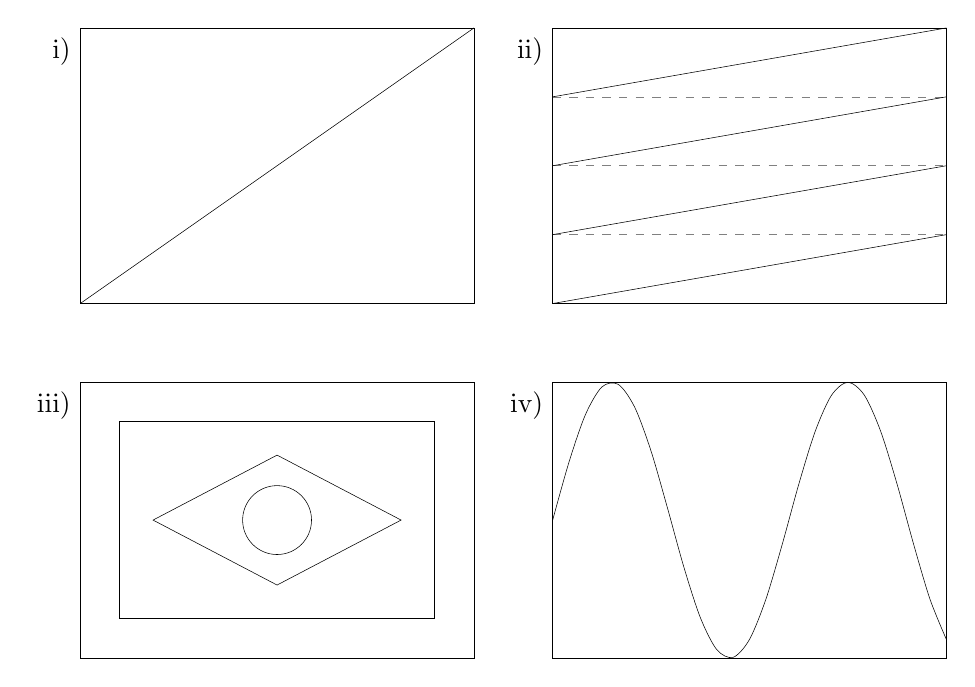
\begin{tikzpicture} [every path/.style={very thin}]
\begin{scope}
\draw (0,0) rectangle (5,3.5) node [below left, xshift=-5 cm,\currentcolor] {i)};;
\draw (0,0) -- (5,3.5);
\end{scope}


\begin{scope} [xshift=6cm]
\draw (0,0) rectangle (5,3.5) node [below left, xshift=-5 cm,\currentcolor] {ii)};
\draw [dashed, help lines] (0,3.5*3/4) -- (5,3.5*3/4); 
\draw (5,3.5) -- (0,3.5*3/4);
\draw [dashed, help lines] (0,3.5*2/4) -- (5,3.5*2/4);
\draw (5,3.5*3/4) -- (0,3.5*2/4);
\draw [dashed, help lines] (0,3.5*1/4) -- (5,3.5*1/4);
\draw (5,3.5*2/4) -- (0,3.5*1/4);
\draw (5,3.5*1/4) -- (0,0);
\end{scope}

\begin{scope} [yshift=-4.5cm]
\draw (0,0) rectangle (5,3.5) node [below left, xshift=-5 cm, \currentcolor] {iii)};;
\draw (.5,.5) rectangle (4.5,3);
\draw (.5+1.7/4,1.75) -- (2.5,.5+1.7/4) -- (4.5-1.7/4,1.75) -- (2.5,3-1.7/4) -- cycle;
\draw (2.5,1.75) circle (0.4375);
\end{scope}

\begin{scope}[xshift =6cm, yshift=-4.5cm]
\draw (0,0) rectangle (5,3.5) node [below left, xshift=-5 cm,\currentcolor] {iv)};;
\draw plot [domain=0:5, smooth] (\x,{1.75*sin (2*pi*\x/3 r)+1.75});
\end{scope}
\end{tikzpicture}
\end{figure}

\end{enumerate}
\end{task}

\begin{task}{cilindro de GNV}



Na Atividade: GNV discutimos a capacidade do tanque de GNV e a compressibilidade do gás nele colocado. Agora vamos aproveitar esta situação para falar do volume ocupado pelo tanque.

\textbf{Parte 1} Aproximação: cota inferior e cota superior

\begin{figure}[H]
\centering

\noindent\includegraphics[width=200bp]{{100}.png}
\end{figure}
\begin{enumerate}
\item {} 
Aproxime o volume ocupado (em metros cúbicos), por um tanque de GNV de capacidade \(15,5m^3\) como o da figura.

\item {} 
Encontre o menor número que você conseguir que seja certamente maior do que o volume ocupado pelo tanque de GNV. Apresente sua resposta em metros cúbicos e em litros. Use os recursos que julgar conveniente.

\item {} 
Agora encontre o maior número que você conseguir que seja certamente menor que o volume ocupado pelo tanque de GNV. Apresente sua resposta em metros cúbicos e em litros. Use os recursos que julgar conveniente.

\item {} 
Encontre o menor número que você conseguir que seja certamente maior que o volume ocupado pelo tanque de GNV. Apresente sua resposta em metros cúbicos e em litros. Novamente você pode usar os recursos que julgar conveniente para resolver a atividade.

\item {} 
Crie um modelo aproximado do tanque usando figuras conhecidas, busque as fórmulas para o cálculo do volume destas figuras e obtenha uma nova aproximação para o volume do tanque.

\item {} 
Discuta o significado da diferença entre as suas aproximações para o volume do tanque e a capacidade especificada pelo vendedor, de \(15,5m^3\).

\end{enumerate}

\textbf{Parte 2}

Dentre os carros populares, os mais econômicos na cidade fazem \(14 km / l\) usando gasolina e \(10 Km / l\) usando etanol como combustível (Veja a edição de 2018 do \href{http://www.inmetro.gov.br/consumidor/pbe/veiculos\_leves\_2018.pdf}{Programa Brasileiro de Etiquetagem Veicular} do INMETRO).
\begin{enumerate}
\item {} 
Verifique se é financeiramente mais vantajoso usar gasolina ou etanol com os preços atuais no seu município. Use o preço médio para este cálculo*.
\begin{itemize}
\item {} 
Os preços atuais do GNV, da Gasolina e do Etanol no seu município estão no \href{http://anp.gov.br/preco/prc/Resumo\_Por\_Municipio\_Index.asp}{Sistema de Levantamento de Preços da ANP}.

\end{itemize}

\item {} 
É corrente entre usuários de carros com motor FLEX utilizar a regra dos 70\% para saber se é mais vantajoso usar etanol ou gasolina (Veja por exemplo: \href{http://www.calculoexato.net/calculadora-flex-gasolina-x-alcool/}{calculadora}). A regra funciona assim: se o preço do etanol for até 70\% do preço da gasolina, deve-se comprar etanol, acima desse percentual deve-se comprar gasolina. É claro que o valor 70\% é aproximado. Explique como ela foi obtida.

\end{enumerate}

Estes mesmos veículos fariam aproximadamente 16 Km / m\(\sp{\text{3}}\) de GNV. Digamos que você saiba que o serviço de instalação pode ser financiado em até 10 vezes de R\$ 420,00 para o seu carro.
\begin{enumerate}
\item {} 
Quantos quilômetros você precisaria rodar em média por dia para que você consiga pagar a instalação com a economia de combustível proveniente do uso do GNV. Use o preço médio para este cálculo?

\item {} 
Os motores dos veículos a base destes combustíveis fósseis, como GNV, gasolina e etanol funcionam a base de combustão. Isto é, consomem oxigênio e liberam gás carbônico e água. Um motor regulado libera aproximadamente 2392 gramas de \(CO_2\) por de gasolina e 2252 gramas de CO\_2 por quilograma de GNV. Qual dos dois combustíveis emite menos CO\_2 por cada quilômetro rodado? Considerando que a densidade do GNV no motor do veículo é de aproximadamente 0,8 Kg / m\(\sp{\text{3}}\).

\end{enumerate}
\end{task}

\begin{task}{aproximando pi}



\textbf{Parte 1}

Existe uma constante muito importante na matemática chamada  \(\pi\) (lê-se pi), que aparece nas fórmulas do comprimento da circunferência, área do círculo, volume da esfera, funções trigonométricas e muitas outras.

O valor dessa constante fundamental na matemática é definido como: a metade do comprimento da circunferência de raio um. Nesta atividade usaremos a fórmula da área do círculo para obter uma aproximação de \(\pi\).

Lembre-se que a fórmula para a área de um círculo de raio \(r\) é  \(\pi.r^2\). Dessa forma, para obter uma aproximação de \(\pi\), basta aproximar a área de um círculo e dividir o resultado obtido por \(r^2\). É o que faremos. Mas como aproximar a área de um círculo? Vamos fazer isso usando a área de figuras já conhecidas.
\begin{enumerate}
\item {} 
Desenhe um círculo em um papel em branco (usando uma forma circular ou um compasso) e meça o seu diâmetro. Feito isso, use uma régua para quadricular o papel com quadrados de tamanho um décimo do diâmetro do círculo, como ilustrado a seguir.

\begin{figure}[H]
\centering

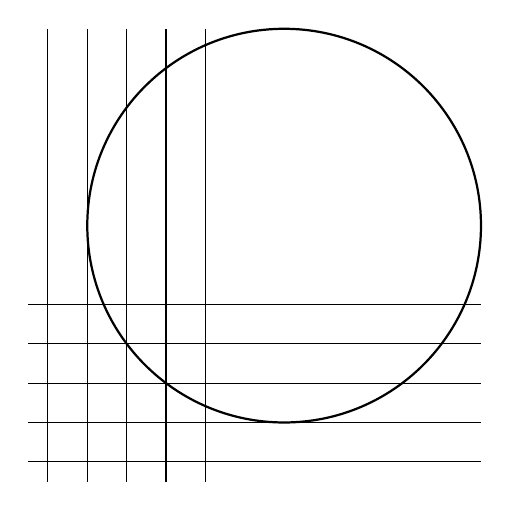
\begin{tikzpicture}[scale=2.5]

\draw [\currentcolor, thick](0,0) circle (1cm);
\foreach \x in {-1.2,-1,-0.8,-0.6,-0.4} \draw (-1.3,\x) -- (1,\x);
\foreach \x in {-1.2,-1,-0.8,-0.6,-0.4} \draw (\x,-1.3) -- (\x,1);

\end{tikzpicture}\end{figure}

\item {} 
Qual a medida da área de um quadradinho do quadriculado que você fez?

\item {} 
Com essa figura, pinte todos os quadradinhos que estão inteiramente contidos no círculo. Qual é a área da região colorida? Agora pinte todos os quadradinhos que têm intersecção não vazia com o círculo. Qual é a área da nova região colorida. Com esses cálculos é possível concluir que a área do círculo está entre que números? Dê uma estimativa para a área do círculo.

\item {} 
Sabendo que a fórmula da área do círculo é \(\pi.r^2\) e usando os cálculos realizados no item anterior, apresente estimativas para \(\pi\), uma menor e outra maior do que o valor de \(\pi\). Algo como: “\(\pi\) é maior do que \_\_\_\_  e menor do que \_\_\_\_”.

\item {} 
Compare os resultados obtidos neste experimento com o valor de \(\pi\) que você conhece.

\item {} 
Que alteração poderia ser feita no processo desse experimento para melhorar a aproximação obtida para \(\pi\)?

\end{enumerate}

\textbf{Parte 2}

A imprecisão do método utilizado na Parte 1 está na limitação do desenho, que, especialmente à medida que os quadradinhos diminuem, dificulta a decisão sobre alguns quadradinhos terem ou não interseção com o círculo. Desta vez, usaremos outro procedimento para aproximar o valor de \(\pi\), sem incorrer neste tipo de imprecisão.
\begin{enumerate}
\item {} 
Calcule o lado do quadrado e do octógono regular inscritos em um círculo de raio um (como na figura abaixo).

\begin{figure}[H]
\centering

\begin{tikzpicture} [scale=3.5, every path/.style={very thick}]


\draw (0,0) circle (1cm);
\draw [color=atento!80] (0.7071,0.7071) -- ++(-90:2*0.7071) -- ++(-180:1.4142) -- ++(-270:1.4142) -- cycle;
\draw [color=destacado!80] (0.7071,0.7071) -- ++(157.5:0.76535) -- ++(202.5:0.76535) -- ++(247.5:0.76535) -- ++(292.5:0.76535) -- ++(337.5:0.76535) -- ++(22.5:0.76535) -- ++(67.5:0.76535) -- cycle;
\draw [color=primario!80] (0.7071,0.7071) -- ++(-56.25:0.39017) -- ++(-56.25-22.5:0.39017) -- ++(-56.25-22.5-22.5:0.39017) -- ++(-56.25-22.5-22.5-22.5:0.39017) -- ++(-56.25-22.5-22.5-22.5-22.5:0.39017) -- ++(-56.25-22.5-22.5-22.5-22.5-22.5:0.39017) -- ++(-56.25-22.5-22.5-22.5-22.5-22.5-22.5:0.39017) -- ++(-56.25-22.5-22.5-22.5-22.5-22.5-22.5-22.5:0.39017) -- ++(-56.25-22.5-22.5-22.5-22.5-22.5-22.5-22.5-22.5:0.39017) -- ++(-56.25-22.5-22.5-22.5-22.5-22.5-22.5-22.5-22.5-22.5:0.39017) -- ++(-56.25-22.5-22.5-22.5-22.5-22.5-22.5-22.5-22.5-22.5-22.5:0.39017)--++(-56.25-22.5-22.5-22.5-22.5-22.5-22.5-22.5-22.5-22.5-22.5-22.5:0.39017)--++(-56.25-22.5-22.5-22.5-22.5-22.5-22.5-22.5-22.5-22.5-22.5-22.5-22.5:0.39017)--++(-56.25-22.5-22.5-22.5-22.5-22.5-22.5-22.5-22.5-22.5-22.5-22.5-22.5-22.5:0.39017)--++(-56.25-22.5-22.5-22.5-22.5-22.5-22.5-22.5-22.5-22.5-22.5-22.5-22.5-22.5-22.5:0.39017)-- cycle;
\foreach  \x in {0,22.5,45,67.5,90,112.5,135,157.5,180,202.5,225,247.5,270,292.5,315,337.5,360} \draw [very thin,help lines] (0,0) -- ++(\x:1);


\end{tikzpicture}

\end{figure}

\item {} 
Calcule a área dessas figuras e use os resultados para estimar o valor de \(\pi\). O valor encontrado é maior ou menor do que \(\pi\)? Compare a aproximação obtida neste item com a obtida na Parte 1 desta atividade. Avalie qualitativamente a melhora da aproximação.

\item {} 
Faça o mesmo agora considerando um hexágono circunscrito ao círculo unitário e estime o valor de \(\pi\) por cima.

\end{enumerate}

Outra forma de estimar el valor de \(\pi\) usando áreas pode ser encontrada no \href{https://www.geogebra.org/m/v2aqzkce}{aplicativo Geogebra: Aproximação de Pi}
\end{task}


\explore{Princípio de Cavalieri}
\label{\detokenize{GE504-8:explorando-principio-de-cavalieri}}\label{\detokenize{GE504-8::doc}}
\begin{task}{Princípio de Cavalieri em 2D}



O Princípio de Cavalieri, objeto de estudo desta seção, apresenta condições para que duas regiões planas (dois sólidos) tenham mesma área ( mesmo volume).
\begin{enumerate}
\item {} 
Use o aplicativo \href{https://ggbm.at/bxrxatwv}{deste link} e o aplicativo \href{https://ggbm.at/gkh7g4y5}{deste link} e tente descrever com as suas palavras o que vem a ser o Princípio de Cavalieri. Registre por escrito a sua descrição.

\item {} 
Use o aplicativo \href{https://ggbm.at/rqpdcc33}{deste link} e veja se a descrição do item anterior ainda serve para este exemplo.

\end{enumerate}
\end{task}

\begin{task}{distância percorrida dada a velocidade instantânea}



A velocidade de um veículo em metros por segundo no intervalo de tempo {[}1,4{]} segundos é dada pela expressão \(v(t) = t^2 - 4t + 5\) cujo gráfico está esboçado na figura.

\begin{figure}[H]
\centering

\begin{tikzpicture}[scale=1.5, every node/.style={scale=1.5}]

\draw [->] (-.1,0) -- (5.5,0) node [above left, scale=0.6] {$t$};
\draw [->] (0,-.1) -- (0,5.5) node [below right, scale=0.6] {$v$};

\foreach \x in {1,...,5} {\draw (\x,.05) -- (\x,-.05)  node [scale=0.5, below] {\x}; \draw (.05,\x) -- (-.05,\x) node [scale=0.5, left] {\x};
}
\node [below left, scale=0.5] at  (-.05,-.05)  {0};

\draw [color=\currentcolor!80, domain=1:4, semithick, smooth] plot  (\x,{(\x)^2 -4*\x+5}) node [color=\currentcolor!80, left, xshift =-0.5cm, yshift=-1cm , scale=0.6] {$v(t)=t^2 - 4t +5$};
\node [ponto, fill=\currentcolor!80, scale=0.7] at (1,2) {} node at (1,2) [above right, scale=0.5] {(1,2)};
\node [ponto, fill=\currentcolor!80, scale=0.7] at (4,5) {} node at (4,5) [above right, scale=0.5] {(4,5)};



\end{tikzpicture}
\end{figure}

\begin{figure}[H]
\centering

\begin{tikzpicture}[scale=1.5, every node/.style={scale=1.5}]

\fill [\currentcolor!50, opacity=0.3, domain =1:4, variable=\x] (1,0) -- plot  (\x,{(\x)^2 -4*\x+5}) -- (4,0) -- cycle;


\draw [->] (-.1,0) -- (5.5,0) node [above left, scale=0.6] {$t$};
\draw [->] (0,-.1) -- (0,5.5) node [below right, scale=0.6] {$v$};

\foreach \x in {1,...,5} {\draw (\x,.05) -- (\x,-.05)  node [scale=0.5, below] {\x}; \draw (.05,\x) -- (-.05,\x) node [scale=0.5, left] {\x};
}
\node [below left, scale=0.5] at  (-.05,-.05)  {0};

\draw [color=\currentcolor!80, domain=1:4, semithick] plot  (\x,{(\x)^2 -4*\x+5}) node [color=\currentcolor!80, left, xshift =-0.5cm, yshift=-1cm , scale=0.6] {$v(t)=t^2 - 4t +5$};
\node [ponto, fill=\currentcolor!80, scale=0.7] at (1,2) {} node at (1,2) [above right, scale=0.5] {(1,2)};
\node [ponto, fill=\currentcolor!80, scale=0.7] at (4,5) {} node at (4,5) [above right, scale=0.5] {(4,5)};


\end{tikzpicture}\end{figure}

É um fato conhecido da física que a distância percorrida pelo veículo entre os instantes \(t = 1\) segundo e \(t = 4\) segundos é dado pela área da região limitada pelo gráfico da função velocidade, pelo eixo \(t\) e pelas retas verticais \(t = 1\) e \(t = 4\) (região hachurada na figura).
\begin{enumerate}
\item {} 
Obtenha um método para aproximar a distância percorrida com erro tão pequeno quanto desejado.

\item {} 
Reveja a atividade anterior e busque argumentar pela validade do Princípio de Cavalieri usando a estratégia adotada no item a) desta atividade.

\end{enumerate}
\end{task}

\begin{task}{volume de concreto de uma barragem}

(Derivada da atividade Staumauer de \href{https://www.geogebra.org/u/lindner}{Andreas Lindner} disponível nos materiais do GeoGebra)



A figura mostra um modelo de barragem que pretende-se construir em concreto. Para isso será necessário conhecer o volume da barragem pronta. O responsável pelo projeto informou que ela tem 92m de comprimento, 24m de altura, que todas as seções transversais são retângulos, que ao pé da parede a largura é de 16m, e no topo é de 4,67m de largura e que a espessura da parede aumenta exponencialmente para cima. Garanta que não faltará concreto para a construção! Melhor sobrar do que faltar.

\begin{figure}[H]
\centering

\noindent\includegraphics[width=400bp]{{105}.png}
\end{figure}
\begin{enumerate}
\item {} 
Obtenha a função que a cada altura z da parede associa a largura da parede naquela altura.

\item {} 
Obtenha uma estimativa inicial para o volume da barragem. A ordem de grandeza basta aqui.

\item {} 
Obtenha uma aproximação melhor que a anterior. Tente fazer de modo que possa ser estabelecido um algoritmo que sirva para o cálculo de aproximações sucessivas.

\end{enumerate}
\end{task}


\arrange{Princípio de Cavalieri}
\label{\detokenize{GE504-9:organizando-as-ideias-principio-de-cavalieri}}\label{\detokenize{GE504-9::doc}}
A imagem apresenta duas retas tracejadas paralelas, um retângulo (à esquerda), um paralelogramos não retângulo ao centro e uma outra figura formada por duas linhas curvas e dois segmentos de reta sobre as retas tracejadas. Em todas elas, se traçarmos uma reta paralela às retas tracejadas obteremos segmentos de comprimento 3cm na região por elas limitada.

\begin{figure}[H]
\centering

\begin{tikzpicture}%[scale=, every node/.style={scale=}]

\draw (0,1) -- (3,1) node [midway, scale=0.8, below] {3};
\draw [xshift=4cm] (0.5,1) -- (3.5,1) node [midway, scale=0.8, below] {3};
\draw [xshift =10cm](0.745,1) -- (3.745,1) node [midway, scale=0.8, below] {3};

\draw [, color=\currentcolor](0,0) rectangle (3,4);
\draw [xshift=4cm, color=\currentcolor] (0,0) -- (3,0) -- (5,4) -- (2,4) -- cycle;
\draw [xshift =10cm, color=\currentcolor] (0,0) -- (3,0) .. controls (4,0.5) and (4,1.5) .. (3,2) .. controls (2,2.5) and (2,3.5) .. (3.5,4) -- (0.5,4) .. controls (-1, 3.5) and (-1, 2.5) .. (0,2) .. controls (1,1.5) and (1,0.5) .. (0,0)
;



\end{tikzpicture}
\end{figure}

As áreas dos dois quadriláteros são iguais pois ambos são paralelogramos de mesma base e mesma altura. Como você já deve imaginar da discussão as atividades iniciais desta seção a área da terceira região também coincide com as duas anteriores. Para esta e outras situações usamos o Princípio de Cavalieri.

\textbf{Princípio de Cavalieri (versão do plano):} Suponha que duas regiões em um plano estão compreendidas entre duas retas paralelas. Se toda reta paralela a essas duas retas intersecta as regiões em segmentos de comprimentos iguais, então as duas regiões têm áreas iguais.

A versão tridimensional é inteiramente análoga, mas trata das áreas das seções e volumes dos sólidos onde a versão plana trata de comprimentos das seções e áreas das regiões.

Todos concordamos que pilhas de formas diferentes formadas com as mesmas peças, têm o mesmo volume. O Princípio de Cavalieri é a situação limite deste argumento quando as alturas das peças tende a zero. \href{https://ggbm.at/kdzfw7xd}{Neste aplicativo} você pode manipular os sólidos e melhorar a sua visualização.

\begin{figure}[H]
\centering

\noindent\includegraphics[width=400bp]{{107}.png}
\end{figure}

\textbf{Princípio de Cavalieri (versão do espaço):} Suponha que dois sólidos no espaço estão compreendidos entre planos paralelos. Se todo plano paralelo a estes dois planos intersectar os sólidos em regiões de áreas iguais, então os dois sólidos têm volumes iguais.

Uma primeira aplicação do Princípio de Cavalieri é o cálculo do volume de cilindro oblíquos. Em um cilindro oblíquo todas as seções por um plano paralelo às bases resultam em regiões congruentes às bases. Por isso, e pelo Princípio de Cavalieri, o volume de qualquer cilindro oblíquo coincide com o volume do cilindro reto de mesma área da base e mesma altura. Portanto, o volume dos cilindros oblíquos também são dados por área da base vezes altura. A figura mostra o caso particular em que este cilindro oblíquo tem base triangular.

\begin{figure}[H]
\centering

\noindent\includegraphics[width=400bp]{{108}.png}
\end{figure}

\textbf{Atenção:} Não confunda a altura do prisma oblíquo com o comprimento de suas arestas laterais.


\practice{}
\label{\detokenize{GE504-10::doc}}\label{\detokenize{GE504-10:praticando}}
\begin{task}{reflexões sobre perímetros e áreas de triângulos}



\textbf{Parte 1}

Na figura, as retas \(r\) e \(s\) são paralelas e os segmentos \(BC\) e \(B'C'\) são congruentes.

\begin{figure}[H]
\centering

\begin{tikzpicture}[scale=1.5, every node/.style={scale=2}]

\draw [fill=\currentcolor!80, color=\currentcolor, opacity=0.4] (1,0) -- (1.75,3) -- (2.5,0) -- cycle;

\draw [fill=\currentcolor!80, color=\currentcolor, opacity=0.4] (3,0) -- (4.75,3) -- (4.5,0) -- cycle;

\foreach \x in {(1,0),(1.75,3),(2.5,0),(3,0),(4.5,0)} \node [ponto] at \x {};

\foreach \x/\y/\z in {(1,0)/B/below,(1.75,3)/A/above, (2.5,0)/C/below,(3,0)/B'/below,(4.5,0)/C'/below} \node  [\z, scale=0.5]  at \x {$\y$};

\node [ponto, color=destacado] at (4.75,3) {} node [color=destacado, above, scale=0.5] at (4.75,3) {$A'$};

\draw (0,0) -- (5,0) node [above right, pos=0, scale=0.5] {$s$};
\draw (0,3) -- (5,3) node [above right, pos=0, scale=0.5] {$r$};

\end{tikzpicture}
\end{figure}
\begin{enumerate}
\item {} 
Qual dos triângulos têm a maior área, \(ABC\) ou \(A'B'C'\)? Explique a sua resposta.

\item {} 
Dentre todos os triângulos que se pode formar movendo A’  sobre a reta \(r\), qual deles tem menor perímetro? Justifique. E o de perímetro máximo?

\end{enumerate}

\textbf{Parte 2}

Seja \(H\) a distância entre as retas \(r\) e \(s\) e considere uma reta \(t\) paralela a \(r\) e a \(s\), que dista \(h\) de \(r\) e intersecta os lados dos triângulos em \(XY\) e \(X'Y'\) como na figura.

\begin{figure}[H]
\centering

\begin{tikzpicture}[scale=1.5, every node/.style={scale=2}]

\draw [fill=\currentcolor!80, color=\currentcolor, opacity=0.4] (1,0) -- (1.75,3) -- (2.5,0) -- cycle;

\draw [fill=\currentcolor!80, color=\currentcolor, opacity=0.4] (3,0) -- (4.75,3) -- (4.5,0) -- cycle;

\foreach \x in {(1,0),(1.75,3),(2.5,0),(3,0),(4.5,0)} \node [ponto] at \x {};

\foreach \x/\y/\z in {(1,0)/B/below,(1.75,3)/A/above, (2.5,0)/C/below,(3,0)/B'/below,(4.5,0)/C'/below} \node  [\z, scale=0.5]  at \x {$\y$};

\node [ponto, color=destacado] at (4.75,3) {} node [color=destacado, above, scale=0.5] at (4.75,3) {$A'$};

\draw (0,0) -- (7,0) node [above right, pos=0, scale=0.5] {$s$};
\draw (0,3) -- (7,3) node [above right, pos=0, scale=0.5] {$r$};

\draw [help lines] (0,2) -- (7,2);
\draw [help lines] (5.5,3) -- (5.5,2) node [midway, right, scale=0.5, black] {$h$};
\draw [help lines] (6.5,3) -- (6.5,0) node [midway, right, scale=0.5, black] {$H$};
\node [ponto, atento, scale=0.7] at (6.5,2) {};

\draw [destacado, thick] (1.5,2) -- (2,2) node [pos=0, ponto] {} node [pos=0, above left, scale=0.5, black] {$X$} node [pos=1, ponto] {} node [pos=1, above right, scale=0.5, black] {$Y$};

\draw [destacado, thick] (4.17,2) -- (4.67,2) node [pos=0, ponto] {} node [pos=0, above left, scale=0.5, black] {$X'$} node [pos=1, ponto] {} node [pos=1, above right, scale=0.5, black] {$Y'$};
\end{tikzpicture}
\end{figure}
\begin{enumerate}
\item {} 
Mostre que, seja lá qual for a distância \(h\), os segmentos \(XY\) e \(X'Y'\) são congruentes.

\item {} 
Seja \(\mathcal{A}\) = Área(\(ABC\)), use o Princípio de Cavalieri para calcular a Área(\(A'B'C'\)).

\item {} 
Calcule Área(\(AXY\)) / Área(\(ABC\)) em termos de \(h\) e de \(H\).

\end{enumerate}
\end{task}

\begin{task}{volume da pirâmide}



\textbf{Parte 1}

O tetraedro de vértice \(V\) e base \(ABC\) da figura possui arestas de comprimentos \(AB\), \(BC\), \(CA\), \(VA\), \(VB\) e \(VC\) respectivamente iguais a 8, 9, 10, 18, 18, 19 cm e altura \(H\) cm. Foi traçado um plano paralelo ao plano \(ABC\) a uma distância \(h\) do ponto \(V\) intersectando o tetraedro no triângulo \(XYZ\) como na figura.

\begin{figure}[H]
\centering

\noindent\includegraphics[width=300bp]{{112}.png}
\end{figure}
\begin{enumerate}
\item {} 
Explique por que o triângulo \(XYZ\) é semelhante ao triângulo \(ABC\) com razão de semelhança \(h / H\).

\item {} 
Calcule a razão Área(\(XYZ\)) / Área(\(ABC\)) em função de \(h\) e \(H\).

\end{enumerate}

\textbf{Parte 2}

Dois tetraedros com áreas iguais em suas bases e alturas iguais têm volume iguais.

Os tetraedros da figura têm bases \(ABC\) e \(A'B'C'\) de mesma área e possuem alturas iguais. Nesta atividade você vai justificar que eles possuem volumes iguais mesmo sem conhecer a fórmula para o volume de um tetraedro.

\begin{figure}[H]
\centering

\noindent\includegraphics[width=300bp]{{113}.png}
\end{figure}
\begin{enumerate}
\item {} 
Assim como na parte anterior, os triângulos \(XYZ\) e \(X'Y'Z'\) são determinados pela interseção do tetraedro original por um plano paralelo aos planos das bases que dista \(h\) dos vértices. Explique por que os triângulos \(XYZ\) e \(X'Y'Z'\) têm áreas iguais.

\item {} 
Use o Princípio de Cavalieri para explicar por que os tetraedros \(V-ABC\) e \(V-A'B'C'\) têm volumes iguais.

\end{enumerate}

\textbf{Parte 3}

Qualquer tetraedro é parte de um prisma triangular formado por outros dois tetraedros de mesmo volume que o tetraedro original.
\begin{enumerate}
\item {} 
Use o aplicativo \href{https://ggbm.at/shmk9dkj}{deste link} para montar o prisma triangular com os três sólidos apresentados.

\item {} 
Como você nomearia estes sólidos dados?

\item {} 
Explique por que os sólidos dados têm mesmo volume (reveja os resultados dos itens anteriores, se necessário).

\end{enumerate}

\textbf{Parte 4}

A sequência de figuras, apresenta uma demonstração sem palavras de um fato matemático.

\begin{figure}[H]
\centering

\noindent\includegraphics[width=430bp]{{114-115---121}.png}
\end{figure}

Portanto,

\begin{figure}[H]
\centering

\noindent\includegraphics[width=400bp]{{122123}.png}
\end{figure}
\begin{enumerate}
\item {} 
Que fato matemático está sendo justificado na sequência de figuras? Em que sentido as igualdades são verdadeiras?

\item {} 
Explique a construção realizada em cada um dos passos. Explique com cuidado especial as “igualdades” entre os tetraedros.

\end{enumerate}
\end{task}

\begin{task}{volume da esfera}



A figura mostra um hemisfério de raio \(r\) (metade de uma bola) e um cilindro de raio e altura iguais a \(r\) de onde foi removido um cone de mesma base e altura que o cilindro (chamaremos este sólido de anticlépsidra).

\begin{figure}[H]
\centering

\noindent\includegraphics[width=200bp]{{124}.png}
\end{figure}
\begin{enumerate}
\item {} 
Descreva a figura formada na seção da bola por um plano que está a uma distância \(h\) do centro.

\item {} 
Descreva a figura formada na seção da anticlépsidra por um plano que está a uma distância \(h\) do plano da base.

\item {} 
As seções têm mesma área?

\item {} 
Explique por que o volume da esfera de raio \(r\) é \(4/3 \pi.r^3\). Você pode usar aqui que o volume do cone é (1/3).(Área da base) x (altura) e que o volume do cilindro é (Área da base) x (altura).

\end{enumerate}
\end{task}


\exercise{}
\label{\detokenize{GE504-E:exercicios}}\label{\detokenize{GE504-E::doc}}\begin{enumerate}
\item {} 
(OBMEP 2018) Alice colocou um litro (1000 \(cm^3\)) de água em uma jarra  e  mediu  o  nível  da  água.  Depois  ela  colocou  um  objeto  maciço  de  prata  na  jarra  e  mediu  novamente  o  nível  da  água, conforme a figura. A massa de um centímetro cúbico de prata é 10,5 gramas. Qual é a massa desse objeto?

\end{enumerate}

\begin{figure}[H]
\centering

\noindent\includegraphics[width=200bp]{{Screenshot_from_2018-12-07_21-01-39}.png}
\end{figure}
\begin{enumerate}
\item {} 
Considere duas garrafas, uma com água e outra com óleo, e dois cubos visualmente idênticos (com as mesmas dimensões), um de aço e outro de chumbo. Ao submergir os cubos, um em cada garrafa, qual líquido desloca mais, a água ou o óleo?

\item {} 
Um copo possui marcas de arroz e de farinha com numerações em níveis diferentes. Porém os números não possuem unidades associadas. Esses números podem corresponder a medidas de volume? E de massa?

\item {} 
Use um copo medida graduado de cozinha para estimar o volume de um ovo. Descreva a sua estratégia, justificando sua validade. Essa experiência também permite estimar a massa do ovo.

\item {} 
Um objeto qualquer que tenha seu volume alterado terá necessariamente também sua massa alterada? Justifique sua resposta.

\item {} 
Um conhecido quebra cabeça é feito a partir de 27 pequenos cubos presos por um fio (Figura x) que podem ser organizados como um único cubo maior (Figura y). Relacione o volume do quebra cabeça nas duas configurações apresentadas: desmontado e montado.

Figura Figura

\item {} 
Um cilindro de gás do tamanho de uma pessoa foi capaz de encher balões suficientes para preencher um cômodo inteiro. Por que não houve conservação de volume?

\item {} 
Fechamos duas garrafas de refrigerante consumidas até a metade por um longo período. Uma delas foi fechada somente colocando a tampa e outra amassando a garrafa antes de tampá-la. Após alguns dias em qual das garrafas o líquido restante perdeu mais gás?

\item {} 
Na feira há duas barracas que vendem feijão de corda. Na primeira barraca vende-se a medida de uma lata vazia de leite condensada por R\$ 2,00. Na segunda o preço de cada medida é de R\$ 3,00, mas neste caso a medida é uma cambuca de plástico. Escolha qual das seguintes estratégias permitiria determinar com precisão o preço de um kilo de feijão em cada barraca.
\#. Comprar R\$ 10,00 em cada barraca e comparar o tamanho das porções.
\#. Comprar uma medida em cada barraca e pesar as porções numa balança e subtrair os resultados.
\#. Comprar uma medida em cada barraca e pesar as porções numa balança e dividir cada resultado pelo preço.
\#. Comprar uma medida em cada barraca, pesar as porções numa balança e dividir o preço pelo peso de cada porção.
Fonte: \url{https://www.directoalpaladar.com.mx/ingredientes-y-alimentos/lo-que-necesitas-saber-del-tofu}

\item {} 
Ligamos para dois fornecedores de feijões e queremos decidir de qual deles compraremos. O primeiro nos fornece o preço medido em termos de garrafas pet de refrigerante. O segundo, contudo nos informa o preço por sacos de feijão. Qual pergunta poderíamos fazer ao segundo fornecedor para tomar a decisão: quantos quilos tem cada saco? ou quantos litros tem cada saco?

\item {} 
A figura a seguir representa um cubo formado por cubos menores. Quantos cubos menores são necessários para formar o cubo da figura?
FIGURA

\item {} 
Qual é a(s) dimensão(ões) relevante para a compra de uma corda? E para a compra de um tecido? E para a compra de gás ou gasolina?

\item {} 
Quantos cubos foram usados para o arranjo tridimensional da figura a seguir?
FIGURA

\item {} 
Uma tinta deve ser aplicada com espessura de 0.1 mm em uma parede retangular de 3m de altura e 6m de largura. Qual a quantidade mínima de tinta que deve ser comprada?

\item {} 
(OBMEP 2017) Vários quadrados foram dispostos um ao lado do outro, em ordem crescente de tamanho, formando uma figura com 100cm de base. O lado do maior quadrado mede 20cm. Qual é o perímetro da figura formada por esses quadrados?

FIGURA

\item {} 
São dadas peças de tamanho 2 por 3 para cobrir um retângulo 5 por 7, como na figura.

FIGURA
\begin{enumerate}
\item {} 
Faça uma figura da cobertura sem sobreposição indicando os cortes necessários em cada peça.

\item {} 
Preencha a tabela com os cortes

\end{enumerate}

\begin{table}[H]
\centering
\begin{tabu} to \textwidth{|c|c|c|c|}
\hline
\thead
Tipo de corte & Área da peça & núm. de peças usadas & área acumulada \\
\hline
figura & & & \\
\hline
figura & & & \\
\hline
figura & & & \\
\hline
figura & & & \\
\hline
\end{tabu}
\end{table}

\item {} 
A partir do desenho da planta de organização de caixas de produtos num estante industrial, a altura da pilha e o número de produtos em cada caixa; deduzir o número total de produtos transportados na estante.

FIGURA

\item {} 
Em quais das figuras a seguir o volume destacado é de \(\frac{1}{2}m^3\)?

\item {} 
Um jogo de blocos de montar possui blocos em forma de paralelepípedos de lados: 2, 4 e 5. Qual é o lado do menor cubo que podemos construir com esses blocos?

\item {} 
Assinale as características mínimas que precisamos conhecer para determinarmos um prisma a menos de congruência.
* altura,
* número de lados do polígono da base,
* área da base,
* uma aresta lateral,
* todas as arestas laterais,
* comprimentos dos lados do polígono da base,
* ângulo entre uma aresta lateral e o plano de uma das bases.
* ângulos internos do polígono da base.
* polígono da base.

\item {} 
Quais dos cilindros a seguir estão determinados a menos de congruência.
\begin{enumerate}
\item {} 
Figura com cilindro circular reto com raio e altura dados.

\item {} 
Figura com cilindro oblíquo com ângulo do eixo com o plano e altura dados.

\item {} 
Figura com cilindro circular reto com área da base e área lateral dados.

\item {} 
Figura com cilindro circular reto com planificação e as dimensões do retângulo formado na planificação.

\item {} 
Figura com cilindro circular oblíquo com raio e comprimento  do eixo dados.

\end{enumerate}

\item {} 
(Enem 2001)  Um fabricante de brinquedos recebeu o projeto de uma caixa que deverá conter cinco pequenos sólidos, colocados na caixa por uma abertura em sua tampa. A figura representa a planificação da caixa, com as medidas dadas em centímetros.

\end{enumerate} 
% 
\renewcommand\chapterillustration{abertura-perspectiva2.jpeg}
\renewcommand\chapterwhat{Representações em Matemática (semió-
tica): exemplos, aspectos cognitivos e cultu-
rais; projeções em perspectiva: conceitua-
lização via definição 3D, propriedades com

justificativas, aplicações (pinturas, ilusões

de ótica); projeções paralelas: conceitua-
lização, propriedades e aplicações (planta

baixa, mapa de fuga, vistas e ilustrações
em áreas diversas).}

\renewcommand\chapterbecause{As projeções em perspectiva fornecem um modelo matemático que auxilia na compre-
ensão de como vemos, comunicamos e inte-
ragimos com o mundo. Já as projeções pa-
ralelas fornecem uma representação mais

simples e fácil de se entender e, assim, elas

têm sido utilizadas para a confecção de ilus-
trações em várias áreas: Arquitetura, En-
genharia, Biologia, etc. Além disso, no dia

a dia, é importante, por exemplo, saber in-
terpretar diagramas 2D de objetos 3D que

descrevem como montar uma cama, colocar
um cartucho em uma impressora, abrir a
porta de emergência do avião, descobrir a
saída de emergência mais próxima em um
hotel, etc.}

\chapter{Vistas ortogonais e representações em perspectiva}
\label{\detokenize{GE301::doc}}\label{\detokenize{GE301:vistas-ortogonais-e-representacoes-em-perspectiva}}

\mbox{}\thispagestyle{empty}\clearpage

\thispagestyle{empty}

\begin{center}
Projeto: LIVRO ABERTO DE MATEMÁTICA

\noindent \begin{tabular}{lcccr}
\includegraphics[scale=.15]{impa}& \quad\quad& \includegraphics[width=3cm]{logo} & \quad\quad& \includegraphics[scale=.24]{obmep} 
\end{tabular}
\end{center}

\vspace*{.3cm}

Cadastre-se como colaborador no site do projeto: \url{umlivroaberto.org}

Versão digital do capítulo:

\url{https://www.umlivroaberto.org/BookCloud/Volume_1/master/view/GE301.html}


\begin{tabular}{p{.15\textwidth}p{.7\textwidth}}
Título: & Vistas Ortogonais e Representações em Perspectiva\\
\\
Ano/ Versão: & 2020 / versão 1.0 de \today\\
\\
Editora & Instituto Nacional de Matem\'atica Pura e Aplicada (IMPA-OS)\\
\\
Realização:& Olimp\'iada Brasileira de Matem\'atica das Escolas P\'ublicas (OBMEP)\\
\\
Produção:& Associação Livro Aberto\\
\\
Coordenação:& Fabio Simas, \\
            & Augusto Teixeira (livroaberto@impa.br)\\
\\
  Autores: & Humberto Bortolossi (UFF),\\
        & Lhaylla Crisaff (UFF),\\
             \\
Revisão: & Wanderley Rezende  \\
                
\\
Design: & Andreza Moreira (Tangentes Design) \\
\\
  Ilustrações: & --- \\ 
\\
Gráficos: & Humberto Bortolossi (UFF), \\
		      & Tarso Caldas (Licenciando da UNIRIO)\\

\\
  Capa: & Foto de Raphaël LR, no Unplash \\
  		& https://unsplash.com/photos/5KO0SEN0WRs \\

\end{tabular}

\begin{figure}[b]
\begin{minipage}[l]{5cm}
\centering

{\large Licença:}

  \includegraphics[width=3.5cm]{cc-by-sa1}
\end{minipage}\hfill
\begin{minipage}[c]{5cm}
\centering
{\large Desenvolvido por}

\includegraphics[width=2.5cm]{logo-associacao.jpg}
\end{minipage}
\begin{minipage}[r]{5cm}
\centering

{\large Patrocínio:}
  \vspace{1em}
  \includegraphics[width=3.5cm]{itau}
\end{minipage}
\end{figure}

\mainmatter

\explore{representando o que vemos}
\label{\detokenize{GE301-0::doc}}\label{\detokenize{GE301-0:explorando-representando-o-que-vemos}}
Desde a pré-história, o ser humano tem registrado em pinturas o que ele vê no mundo que o cerca. Na \hyperref[\detokenize{GE301-0:fig-proj-pintura-01}]{Figura \ref{\detokenize{GE301-0:fig-proj-pintura-01}}}, por exemplo, temos, em (a), um desenho de leões e bisões na Caverna de Chauvet na França (com cerca de 30000 anos de idade) e, em (b), uma pintura rupestre no Parque Nacional Serra da Capivara no Piauí (com cerca de 11000 anos de idade).

\begin{figure}[H]
\centering
\capstart

\noindent\includegraphics[width=400bp]{{fig-proj-pintura-01}.jpg}
\caption{Pinturas pré-históricas.}\label{\detokenize{GE301-0:fig-proj-pintura-01}}\label{\detokenize{GE301-0:id25}}\end{figure}

Ao longo da história, seja em paredes, páginas de livros, telas de pintura ou telas de computador, surgiram diversas formas de se representar os objetos tridimensionais que estão em nossa volta. Neste capítulo, estudaremos duas destas formas de representação, importantes por suas aplicações. Para que você possa entender melhor o contexto, iniciaremos com atividades cujo objetivo é levar você a ver como as pessoas representam o que veem e como nossos cérebros interpretam essas representações.
\phantomsection\label{\detokenize{GE301-0:ativ-proj-atelier-geometrico}}
\begin{task}{Atelier geométrico}

Seu professor irá dispor um conjunto de objetos geométricos sobre uma mesa e o objetivo desta tarefa é que você desenhe em uma folha de papel \textbf{o que você vê nesta cena} o mais fielmente que conseguir.

\begin{figure}[H]
\centering

\noindent\includegraphics[width=300bp]{{atelier}.jpg}
\end{figure}

\end{task}
\phantomsection\label{\detokenize{GE301-0:ativ-proj-lobo}}
\begin{task}{É O Lobo!}



Na sua opinião, qual das seis imagens (A), (B), (C), (D), (E) e (F) a seguir melhor representa um lobo? Por quê?

\begin{figure}[H]
\centering
\capstart

\noindent\includegraphics[width=350bp]{{lobo_1}.jpg}
\caption{Seis representações de um lobo.}\label{\detokenize{GE301-0:fig-proj-lobo}}\label{\detokenize{GE301-0:id28}}\end{figure}

\end{task}


\arrange{tudo é uma questão de comunicação!}
\label{\detokenize{GE301-0:organizando-as-ideias-tudo-e-uma-questao-de-comunicacao}}
Em um primeiro momento, você pode achar que a fotografia (A) na \hyperref[\detokenize{GE301-0:fig-proj-lobo}]{Figura \ref{\detokenize{GE301-0:fig-proj-lobo}}} é a “melhor” representação de um lobo. Mas, pense um pouco: “melhor” em que sentido? O “melhor” sempre pressupõe um critério e, por conseguinte, um contexto.

Por exemplo, caso você queira fazer menção a um lobo em uma mensagem de texto enviada por SMS, então certamente a representação (F) é a mais adequada. Agora, imagine que você está escrevendo um livro de Biologia e sua editora lhe disse que, por razões orçamentárias, apenas figuras em “preto e branco” serão aceitas. Neste caso, as representações (B) e (C) parecem ser a melhor opção. E se você estivesse ilustrando um livro infantil? Aí, as representações (D) e (E) poderiam dar um tom artístico mais pessoal ao livro.

A representação (E) pode parecer muito tosca e infantil, mas lembramos aqui uma frase célebre do pintor Pablo Picasso (1881-1973):  “Levei quatro anos para aprender a pintar como Rafael, mas levei a vida toda para aprender a desenhar como uma criança.”.

\begin{figure}[H]
\centering

\includegraphics[width=320bp]{{picasso}.jpg}
\caption{Os touros de Pablo Picasso.}
\label{\detokenize{GE301-0:fig-proj-picasso}}
\label{\detokenize{GE301-0:id29}}
\end{figure}


Do mesmo modo que um lobo pode ser representado de maneiras diferentes, existem diversas representações para os objetos geométricos tradicionais em Matemática (cubos, cilindros, esferas, pirâmides, etc.). Mais ainda, estudiosos descobriram que a forma de representar muda com a idade de uma pessoa.
O filósofo Georges Henri Luquet explica, por exemplo, que o desenho do cilindro do Estágio 2 na \hyperref[\detokenize{GE301-0:fig-proj-escala-mitchelmore}]{Figura \ref{\detokenize{GE301-0:fig-proj-escala-mitchelmore}}} deve-se a uma preponderância de um “realismo intelectual” em relação a um “realismo visual”: a pessoa sabe que um cilindro circular reto têm duas bases circulares e pensa, nesta etapa, que se não registrar estas estas duas bases circulares, o desenho estaria incompleto. Assim, esta pessoa está registrando o que pensa, não o que vê.

\begin{figure}[H]
\centering
\capstart

\noindent\includegraphics[width=400bp]{{cilindros}.jpg}
\caption{Representação de um cilindro em estágios etários diferentes.}\label{\detokenize{GE301-0:fig-proj-escala-mitchelmore}}\label{\detokenize{GE301-0:id30}}\end{figure}

O psicólogo Sergio Morra, por sua vez, argumenta que a complexidade das regras ou estratégias de organização espacial que uma pessoa consegue dominar está restrita pela quantidade de informação que ela pode assimilar e processar simultaneamente, ou seja, pela memória de trabalho. Assim, os desenhos podem ficar “mais realistas” a medida que a memória de trabalho da pessoa aumenta com a idade.

Outro aspecto interessante é que o meio cultural pode influenciar a maneira como uma pessoa representa objetos tridimensionais, como aponta o estudo de Gutierrez (1998). A \hyperref[\detokenize{GE301-0:fig-proj-aspectos-culturais-01}]{Figura \ref{\detokenize{GE301-0:fig-proj-aspectos-culturais-01}}}), por exemplo, mostra como filhos de tecelões, oleiros e fazendeiros de povoados isolados na Índia, entre 8 e 12 anos de idade, com pouca ou nenhuma escolaridade, desenheram cilindros e pirâmides que lhe foram apresentados.

\begin{figure}[H]
\centering
\capstart

\noindent\includegraphics[width=230bp]{{aspectos_culturais}.jpg}
\caption{Influência de fatores culturais na produção de desenhos em perspectiva (Gutierres, 1998)}\label{\detokenize{GE301-0:fig-proj-aspectos-culturais-01}}\label{\detokenize{GE301-0:id31}}\end{figure}

Muitos acham que a habilidade de desenhar é um dom que, quem não tem, nunca irá desenhar bem. Neurocientistas têm mostrado \textbf{que este não é o caso}! De fato, estudos científicos mostram (a) que, como qualquer outra habilidade humana, com prática e dedicação, é possível aprender a desenhar; (b) que habilidades visuais constituem um dos tipos reconhecidos de inteligência humana; (c) que o desenvolvimento das habilidades espaciais desenvolvem outros tipos de habilidades.

Ainda no contexto de objetos geométricos matemáticos, para você ter uma ideia da multiplicidade de representações, considere o problema de representar no plano o globo terrestre modelado como uma esfera. Essas representações nada mais são do que os \index{mapas cartográficos}mapas cartográficos da Geografia! Existem muitos deles, cada um com propriedades e usos específicos! A escolha do mapa depende do que se quer comunicar!

\begin{figure}[H]
\centering
\capstart

\noindent\includegraphics[width=270bp]{{mapas_1}.jpg}
\caption{Mapas cartográficos são representações no plano do globo terrestre modelado como uma superfície esférica.}\label{\detokenize{GE301-0:fig-proj-mapas-cartograficos}}\label{\detokenize{GE301-0:id32}}\end{figure}

Um ponto muito importante para o que se seguirá é ter em mente que, apesar de podermos representar o que vemos de formas diferentes com usos diferentes, certas representações são construídas de maneira bem específicas e, portanto, possuem propriedades que lhe são próprias. Reconhecer, compreender e empregar corretamente estas propriedades são habilidades fundamentais para você se comunicar adequadamente em termos visuais! Este será exatamente o caso das duas representações 2D de objetos 3D obtidas por projeções em perspectivas e projeções paralelas, temas deste capítulo!

A seguinte analogia entre desenho e escrita, inspirada no livro \emph{Desenho e Escrita como Sistemas de Representação} de Analice Dutra Pillar, pode lhe ajudar a perceber a importância de se dar atenção às características específicas de uma determinada representação. Você se comunica por escrito via WhatsApp e, também, ao fazer uma redação no ENEM. No WhatsApp, pela agilidade que é característica deste meio de comunicação, você usa abreviações: “tdb” (tudo bem), “pdc” (pode crer), “obg” (obrigado), etc. Mesmo com abreviações, as pessoas se entendem. Por outro lado, em uma redação do ENEM, exige-se que o texto seja escrito seguindo características específicas, a saber, “de acordo com a modalidade escrita formal da língua portuguesa”: você deve respeitar as regras ortográficas e gramaticais. Analogamente, existem várias maneiras de se desenhar um cubo. Contudo, os desenhos obtidos por projeções em perspectiva e projeções paralelas possuem propriedades específicas. São essas propriedades e suas aplicações que vamos estudar neste capítulo!

\begin{knowledge}{}

O matemático alemão Johann Carl Friedrich Gauss (1777-1855) demonstrou um teorema, o chamado \emph{egregium}, a partir do qual é possível deduzir o seguinte resultado: qualquer representação plana que se faça de um globo terrestre modelado como uma esfera \textbf{sempre} terá algum tipo de distorção, isto é, ela não preservará ângulos ou não preservará áreas ou não preservará distâncias. Na página web \textless{}\url{https://goo.gl/HbLnPW}\textgreater{}, você encontrará um aplicativo que permite visualizar essas distorções para diferentes mapas cartográficos: as curvas fechadas mais espessas (círculos no exemplo da figura a seguir) são, no mapa, as representações de círculos de mesmo raio desenhados sobre a superfície esférica do globo terrestre. A partir da comparação dos formatos relativos dessas curvas (a \index{indicatriz de Tissot}indicatriz de Tissot) é possível ter uma ideia das distorções presentes no mapa.


\begin{figure}[H]
\centering

\noindent\includegraphics[width=50bp]{egregium-qrcode.png}
\end{figure}

\begin{figure}[H]
\centering

\noindent\includegraphics[width=280bp]{{egregium_1}.jpg}
\end{figure}


Existem mapas que preservam um ou outro atributo geométrico. O mapa de Mercator, por exemplo, preserva ângulos (mas não preserva áreas) e possui uma característica adicional útil para a navegação: as curvas de rumo constante sobre a superfície terrestre são representadas por retas neste mapa.
\end{knowledge}


\explore{interpretando o que vemos}
\label{\detokenize{GE301-1::doc}}\label{\detokenize{GE301-1:explorando-interpretando-o-que-vemos}}\phantomsection\label{\detokenize{GE301-1:ativ-proj-interpretando}}
\begin{task}{Será que é?}

\begin{enumerate}
\item {} 
(Ponzo) Observe a \hyperref[\detokenize{GE301-1:fig-proj-ponzo}]{Figura \ref{\detokenize{GE301-1:fig-proj-ponzo}}}. Qual carro é maior na imagem?

\begin{figure}[H]
\centering
\capstart

\noindent\includegraphics[width=300bp]{{ponzo-illusion-04}.jpg}
\caption{Qual carro é maior na imagem?}\label{\detokenize{GE301-1:fig-proj-ponzo}}\label{\detokenize{GE301-1:id14}}\end{figure}

\item {} 
(Shepard) Observe a \hyperref[\detokenize{GE301-1:fig-proj-shepard}]{Figura \ref{\detokenize{GE301-1:fig-proj-shepard}}}. Qual mesa é mais comprida na imagem?

\begin{figure}[H]
\centering
\capstart

\noindent\includegraphics[width=300bp]{{mesa-de-shepard}.jpg}
\caption{Qual mesa é mais comprida na imagem?}\label{\detokenize{GE301-1:fig-proj-shepard}}\label{\detokenize{GE301-1:id15}}\end{figure}

\end{enumerate}
\end{task}


\arrange{ver é uma atividade complexa!}
\label{\detokenize{GE301-1:organizando-as-ideias-ver-e-uma-atividade-complexa}}
Os dois exemplos apresentados na atividade anterior mostram que o ato de ver e compreender uma imagem não se encerra na própria imagem, mas depende da maneira que nosso cérebro processa toda a informação e se ajusta ao estímulo visual.

Psicólogos têm mapeado outras situações onde nosso cérebro faz adequações visuais subjetivas ao contexto: forma, cor, iluminação, distância, localização e movimento. Mais ainda: não só o sistema visual é afetado por ilusões, os demais sentidos também o são. Um exemplo clássico é o Efeito McGurk que mostra \textbf{como o que você vê altera o modo como você ouve}! Experimente você mesmo por meio do \href{https://goo.gl/k241EQ}{vídeo} no YouTube.

\begin{figure}[H]
\centering

\noindent\includegraphics[width=50bp]{{efeito-mcgurk-01}.png}
\end{figure}

O fato de nosso cérebro estar sucetível a estes tipos de ilusões pode parecer um defeito a princípio mas, como mostra o cientista cognitivo Donald Hoffman nesta  \href{https://goo.gl/x5H5oa}{palestra TED}, isto é resultado de um processo evolutivo que garantiu a nossa sobrevivência.


\begin{figure}[H]
\centering

\noindent\includegraphics[width=50bp]{{ted-realidade-02}.png}
\end{figure}



\begin{figure}[H]
\centering
\capstart

\noindent\includegraphics[width=350bp]{{ted-realidade-01}.jpg}
\caption{\href{https://goo.gl/x5H5oa}{Link para o vídeo}}\label{\detokenize{GE301-1:id16}}\end{figure}

Outro aspecto da interpretação de representações 2D de objetos 3D se refere à questão de ambiguidade: um mesmo desenho plano pode ser a representação de objetos tridimensionais diferentes. Considere, por exemplo, a Imagem (A) na \hyperref[\detokenize{GE301-1:fig-proj-ambiguidade-01}]{Figura \ref{\detokenize{GE301-1:fig-proj-ambiguidade-01}}}. Ela pode ser a representação de um cubo visto de cima como na Imagem (B) ou de um cubo visto de baixo como na Imagem (C).

\begin{figure}[H]
\centering
\setlength{\columnsep}{0pt}

\begin{multicols}{3}
\begin{figure}[H]
\raggedleft
\begin{asy}
size(3cm);
currentprojection=orthographic(3,1,.5);

triple a = (0,0,0);
triple b = (1,0,0);
triple c = (1,1,0);
triple d = (0,1,0);

triple e = (0,0,1);
triple f = (1,0,1);
triple g = (1,1,1);
triple h = (0,1,1);

draw (a -- b -- c -- d -- cycle);
draw (e -- f -- g -- h -- cycle);
draw (a -- b -- f -- e -- cycle);
draw (c -- d -- h -- g -- cycle);
\end{asy}
\centering
\\
(A)
\end{figure}

\begin{figure}[H]
\centering
\begin{asy}
size(3cm);
currentprojection=orthographic(3,1,.5);

triple a = (0,0,0);
triple b = (1,0,0);
triple c = (1,1,0);
triple d = (0,1,0);

triple e = (0,0,1);
triple f = (1,0,1);
triple g = (1,1,1);
triple h = (0,1,1);

draw(e -- f -- g -- h -- cycle);
draw(c -- d -- h -- g -- cycle);
draw(b -- c -- g -- f -- cycle);

draw(b -- a --d, dashed);
draw(a -- e, dashed);
\end{asy}
\centering
\\
(B)
\end{figure}

\begin{figure}[H]
\raggedright
\begin{asy}
size(3cm);
currentprojection=orthographic(3,1,.5);

triple a = (0,0,0);
triple b = (1,0,0);
triple c = (1,1,0);
triple d = (0,1,0);

triple e = (0,0,1);
triple f = (1,0,1);
triple g = (1,1,1);
triple h = (0,1,1);

draw(a -- b -- c -- d -- cycle);
draw(a -- b -- f -- e -- cycle);
draw(a -- d -- h -- e -- cycle);

draw(h -- g -- c, dashed);
draw(g -- f, dashed);
\end{asy}
\centering
\\

(C)
\end{figure}
\end{multicols}
\caption{Um cubo visto de cima ou de baixo?}\label{\detokenize{GE301-1:fig-proj-ambiguidade-01}}\label{\detokenize{GE301-1:id17}}\end{figure}

De fato, a Imagem (A) pode até mesmo nem ser a representação de um cubo, como mostra a animação da \hyperref[\detokenize{GE301-1:fig-proj-ambiguidade-02}]{Figura \ref{\detokenize{GE301-1:fig-proj-ambiguidade-02}}}. A Imagem (A) é conhecida como \index{Cubo de Necker}Cubo de Necker, em homenagem ao cristalógrafo Louis Albert Necker (1786-1861) que observou este tipo de ambiguidade em 1832.



\begin{figure}[H]
\centering
\capstart

\noindent\includegraphics[width=200bp]{{ambiguidade-02}.jpg}
\caption{\href{https://goo.gl/CXR6AG}{Versão interativa}}\label{\detokenize{GE301-1:fig-proj-ambiguidade-02}}\label{\detokenize{GE301-1:id18}}\end{figure}

Compreender como vemos e interpretamos representações 2D de objetos 3D obtidas por projeções centrais e paralelas é uma habilidade importante que afeta o modo de nos cuminicarmos e interagirmos com o mundo.

\begin{reflection}{}

Se nosso cérebro distorce os estímos que recebemos do mundo a nossa volta, como saber o que é real?
\end{reflection}

\begin{reflection}{}

Será que uma pessoa que nasceu cega mas que, posteriormente, recuperou sua visão, saberia ver de imediato? Ou seria necessário “ensiná-la a ver”? Como saber, por exemplo, onde a imagem de um objeto termina e a imagem de outro começa?  Esta \href{https://goo.gl/KLdhKg}{palestra TED} discute esses assuntos, mostra a importância do movimento no processo de se “aprender a ver” e conta como o trabalho do neurocientista indiano Pawan Sinha tem mudado a concepção sobre os mecanismos da visão e, também, as vidas de muitas crianças que nasceram cegas.

\begin{figure}[H]
\centering

\noindent\includegraphics[width=50bp]{{ted-aprendendo-a-ver-02}.png}
\end{figure}

\begin{figure}[H]
\centering
\capstart

\noindent\includegraphics[width=350bp]{{ted-aprendendo-a-ver-01}.jpg}
\caption{Palestra TED.}\label{\detokenize{GE301-1:id19}}\end{figure}
\end{reflection}


\begin{reflection}{}

Todas estas questões de representações e significados fazem parte da \index{semiótica}semiótica, disciplina que se ocupa do estudo dos signos e dos processos significativos na natureza e na cultura. Os signos, aqui, não estão restritos à desenhos em uma folha de papel. Eles podem ser qualquer veículo de significação ou representação de um objeto, de um conceito ou de uma ideia, como textos, sons e gestos. Um dos pontos destacados pela semiótica é a distinção entre a representação de algo e este próprio algo. Um exemplo clássico é dada pela pintura na \hyperref[\detokenize{GE301-1:fig-proj-semiotica-01}]{Figura \ref{\detokenize{GE301-1:fig-proj-semiotica-01}}}. O que é que está na pintura? Se você respondeu “cachimbo”, saiba que a legenda em Francês “Ceci n’est pas une pipe.” tem como tradução “Isto não é um cachimbo.”. Segundo o autor da pintura, o surrealista belga René Magritte (1898-1967), ele não poderia escrever o contrário, pois a pintura não é um cachimbo, mas uma representação de um cachimbo. O nome da pintura: “A Traição das Imagens”.

\begin{figure}[H]
\centering
\capstart

\noindent\includegraphics[width=300bp]{{semiotica-01}.jpg}
\caption{Pintura de René Magritte (1898-1967).}\label{\detokenize{GE301-1:fig-proj-semiotica-01}}\label{\detokenize{GE301-1:id20}}\end{figure}

Uma vez que a comunicação se dá por meio de signos, a semiótica é de interesse para muitas áreas: Propaganda, Cinema, Ciência, Literatura, Religião … Em Matemática, o aspecto semiótico é fundamental, como aponta Pinilla (2007):

\begin{quote}
É importante ter em mente que os conceitos matemáticos não existem na realidade concreta. O ponto P, o número 3, adição, paralelismo entre retas não são objetos concretos os quais existem na realidade empírica. Eles são conceitos puros, ideais e abstratos e, desta maneira, eles não podem ser “exibidos empiricamente”, como em outras Ciências. Em Matemática, os conceitos só podem ser representados por um registro semiótico determinado. De fato, em Matemática, não trabalhamos diretamente com os objetos (isto é, com os conceitos), mas com suas representações semióticas.
\end{quote}

Caso você queira saber mais sobre semiótica, recomendamos começar com o livro “O que é semiótica?” da Coleção “Primeiros Passos” da Editora Brasiliense (Santaella, 1998).
\end{reflection}
\phantomsection\label{\detokenize{GE301-1:obs-proj-por-que-estudar-o-assunto}}
\begin{observation}{}

No que se segue, iremos estudar duas formas de representação bem específicas: aquelas obtidas por projeções em perspectiva e projeções paralelas.

As projeções em perspectiva fornecem um modelo matemático para a visão humana e para dispositivos óticos (como câmeras) e o estudo deste modelo auxilia na compreensão de como vemos, comunicamos e interagimos com o mundo. As projeções paralelas, por sua vez, fornecem uma representação mais simples e mais fácil de se entender e, por este motivo, elas têm sido utilizadas para a confecção de ilustrações em várias áreas: Arquitetura, Engenharia, Biologia, Física, etc.

Cabe observar que projeções em perspectiva e paralelas fazem parte das habilidades espaciais as quais, por sua vez, constituem um dos tipos reconhecidos de inteligência humana (Gray et al, 2004), (Gardner, 2011).

As habilidades espaciais são particularmente críticas para profissões relacionadas com as áreas de Ciência, Tecnologia, Engenharia e Matemática (STEM), conforme apontam vários estudos recentes (NRC, 2006), (Utta et al, 2012), (Khine, 2017), (Newcombe, 2017).

Mesmo no dia a dia, é importante, por exemplo, saber interpretar os diagramas 2D de objetos 3D que descrevem como montar uma cama, colocar um cartucho em uma impressora, abrir a porta de emergência do avião, descobrir a saída de emergência mais próxima em um hotel ou em um estádio de futebol (mapa de fuga, saídas de emergência), etc.
\begin{quote}

\begin{figure}[H]
\centering

\noindent\includegraphics[width=400bp]{{planta-baixa-03}.jpg}
\end{figure}

Mapa do circuito de visitação do terceiro andar do Aquário do Rio de Janeiro (fonte: Joselí Maria Silva dos Santos).
\end{quote}

Como veremos, as representações obtidas por projeções em perspectiva e projeções paralelas possuem propriedades bem \textbf{específicas}. Reconhecer e usar essas propriedades adequadamente é importante para você entender e se fazer entender em termos de comunicação visual.
\end{observation}

\begin{reflection}{}

\begin{DUlineblock}{0em}
\item[] \emph{This life five windows of the soul}
\item[] \emph{Distorts the heaven from pole to pole}
\item[] \emph{And leads you to believe a lie}
\item[] \emph{When you see with, no thro’, the eye.}
\end{DUlineblock}

Poema do poeta, pintor, ilustrador e entalhador William Blake (1757-1827).
\end{reflection}


\explore{projeções paralelas e em perspectiva}
\label{\detokenize{GE301-2:explorando-projecoes-em-perspectiva-e-projecoes-paralelas}}\label{\detokenize{GE301-2::doc}}\phantomsection\label{\detokenize{GE301-2:ativ-proj-luz-e-sombras}}
\begin{task}{Luzes e sombras}

Nesta atividade vamos explorar a geometria das sombras! Para isto, você receberá um \emph{kit} cujas sombras deverá analisar: um cubo vazado, um triângulo e um lápis (ou uma caneta ou ainda um canudinho plástico). Você também receberá uma folha de papel A4 ou uma cartolina que servirá como anteparo onde as sombras devem ser projetadas.

\textbf{No que se segue, o termo *configuração* significa uma escolha da posição do objeto, da fonte de luz e do anteparo, conforme o caso.} Assim, o termo \emph{para qualquer configuração} significa para qualquer escolha da posição do objeto, da fonte de luz e do anteparo.

\textbf{Experimentos com um lápis}
\begin{enumerate}
\item {} 
O comprimento da sombra é sempre igual ao comprimento do lápis, independentemente da configuração?
\begin{itemize}
\item {} 
Resposta para o caso da luz da lanterna do celular:

\item {} 
Resposta para o caso da luz do Sol:

\end{itemize}

\item {} 
Existe alguma configuração para a qual o comprimento da sombra seja igual ao comprimento do lápis?
\begin{itemize}
\item {} 
Resposta para o caso da luz da lanterna do celular:

\item {} 
Resposta para o caso da luz do Sol:

\end{itemize}

\item {} 
Segure o seu lápis no meio com as pontas de seus dedos, isto é, considerando o lápis como se fosse um segmento de reta, segure-o pelo seu ponto médio. A sombra das pontas de seus dedos sempre está no meio da sombra do lápis independentemente da configuração?
\begin{itemize}
\item {} 
Resposta para o caso da luz da lanterna do celular:

\item {} 
Resposta para o caso da luz do Sol:

\end{itemize}

\item {} 
Segure o seu lápis, com as pontas de seus dedos, a aproximadamente 1/3 de uma das extremidades. Existe alguma configuração para a qual a sombra das pontas de seus dedos está no meio da sombra do lápis?
\begin{itemize}
\item {} 
Resposta para o caso da luz da lanterna do celular:

\item {} 
Resposta para o caso da luz do Sol:

\end{itemize}

\item {} 
Em qual configuração a sombra do lápis tem a menor área possível?
\begin{itemize}
\item {} 
Resposta para o caso da luz da lanterna do celular:

\item {} 
Resposta para o caso da luz do Sol:

\end{itemize}

\item {} 
Existe alguma configuração onde a sombra não se altere ao mover o lápis em alguma direção? Aqui, \emph{não se altere} signfica ser exatamente a mesma no mesmo lugar.
\begin{itemize}
\item {} 
Resposta para o caso da luz da lanterna do celular:

\item {} 
Resposta para o caso da luz do Sol:

\end{itemize}

\end{enumerate}

\textbf{Experimentos com um triângulo}
\begin{enumerate}
\item {} 
Existe alguma configuração para a qual a sombra do triângulo é um triângulo isósceles?
\begin{itemize}
\item {} 
Resposta para o caso da luz da lanterna do celular:

\item {} 
Resposta para o caso da luz do Sol:

\end{itemize}

\item {} 
Existe alguma configuração para a qual a sombra do triângulo é um triângulo equilátero?
\begin{itemize}
\item {} 
Resposta para o caso da luz da lanterna do celular:

\item {} 
Resposta para o caso da luz do Sol:

\end{itemize}

\item {} 
Em qual configuração a sombra do triângulo tem a menor área possível?
\begin{itemize}
\item {} 
Resposta para o caso da luz da lanterna do celular:

\item {} 
Resposta para o caso da luz do Sol:

\end{itemize}

\item {} 
Existe alguma configuração onde a sombra do triângulo não se altere ao movê-lo em alguma direção? Qual?
\begin{itemize}
\item {} 
Resposta para o caso da luz da lanterna do celular:

\item {} 
Resposta para o caso da luz do Sol:

\end{itemize}

\item {} 
O baricentro de um triângulo é o  ponto de interseção das \index{medianas}medianas do triângulo, isto é, o ponto de interseção dos segmentos de reta que ligam um vértice ao ponto médio do lado oposto. Faça um furo no \index{baricentro}baricentro do seu triângulo, de forma que, ao expô-lo à luz, o ponto correspondente no anteparo ficará iluminado. Este ponto iluminado é baricentro da sombra do triângulo?
\begin{itemize}
\item {} 
Resposta para o caso da luz da lanterna do celular:

\item {} 
Resposta para o caso da luz do Sol:

\end{itemize}

\end{enumerate}

\textbf{Experimentos com um cubo vazado}
\begin{enumerate}
\item {} 
As arestas do cubo vazado têm todas o mesmo tamanho. O mesmo acontece para as sombras destas arestas?
\begin{itemize}
\item {} 
Resposta para o caso da luz da lanterna do celular:

\item {} 
Resposta para o caso da luz do Sol:

\end{itemize}

\item {} 
Existe alguma configuração para a qual a sombra do cubo vazado seja semelhante à imagem da \hyperref[\detokenize{GE301-2:fig-proj-quadrado-vazado-01}]{Figura \ref{\detokenize{GE301-2:fig-proj-quadrado-vazado-01}}}? Em caso afirmativo, é possível manter esta sombra movendo o cubo vazado em alguma direção? Qual?

\begin{figure}[H]
\centering
\capstart

\noindent\includegraphics[width=100bp]{{quadrado-vazado-01_2}.jpg}
\caption{Quadrado vazado.}\label{\detokenize{GE301-2:fig-proj-quadrado-vazado-01}}\label{\detokenize{GE301-2:id1}}\end{figure}
\begin{itemize}
\item {} 
Resposta para o caso da luz da lanterna do celular:

\item {} 
Resposta para o caso da luz do Sol:

\end{itemize}

\item {} 
Arestas que são perpendiculares no cubo vazado têm sombras que são perpendiculares no anteparo de projeção?
\begin{itemize}
\item {} 
Resposta para o caso da luz da lanterna do celular:

\item {} 
Resposta para o caso da luz do Sol:

\end{itemize}

\item {} 
Arestas que são são paralelas no cubo vazado têm sombras que são paralelas no anteparo de projeção?
\begin{itemize}
\item {} 
Resposta para o caso da luz da lanterna do celular:

\item {} 
Resposta para o caso da luz do Sol:

\end{itemize}

\end{enumerate}

\textbf{Outros experimentos}
\begin{enumerate}
\item {} 
Como você faria para determinar a direção de incidência dos raios solares no anteparo?

\item {} 
Posicione o anteparo perpendicularmente à direção de incidência dos raios solares. O que acontece com o formato da sombra do lápis, do triângulo ou do cubo se você movê-los \textbf{paralelamente} à direção de incidência dos raios solares?

\item {} 
Na \hyperref[\detokenize{GE301-2:fig-proj-sombra-vazada-01}]{Figura \ref{\detokenize{GE301-2:fig-proj-sombra-vazada-01}}}, PQRS é sombra de qual face do cubo vazado? Tente responder analisando apenas a figura e, depois, teste a sua resposta com um experimento!

\begin{figure}[H]
\centering
\capstart

\noindent\includegraphics[width=300bp]{{sombra-vazada-01_1}.jpg}
\caption{Sombra vazada.}\label{\detokenize{GE301-2:fig-proj-sombra-vazada-01}}\label{\detokenize{GE301-2:id2}}\end{figure}

\item {} 
Na configuração da \hyperref[\detokenize{GE301-2:fig-proj-sombra-vazada-01}]{Figura \ref{\detokenize{GE301-2:fig-proj-sombra-vazada-01}}}, o que acontece com a sombra do cubo vazada se a lanterna do celular se aproximar do cubo? E se a lanterna se afastar?

\item {} 
Na \hyperref[\detokenize{GE301-2:fig-proj-sombra-vazada-02}]{Figura \ref{\detokenize{GE301-2:fig-proj-sombra-vazada-02}}}, PQRS é sombra de qual face do cubo vazado? Tente responder analisando apenas a figura e, depois, teste a sua resposta com um experimento!

\begin{figure}[H]
\centering
\capstart

\noindent\includegraphics[width=300bp]{{sombra-vazada-02_1}.jpg}
\caption{Sombra vazada.}\label{\detokenize{GE301-2:fig-proj-sombra-vazada-02}}\label{\detokenize{GE301-2:id3}}\end{figure}

\end{enumerate}
\end{task}

\phantomsection\label{\detokenize{GE301-2:ativ-proj-modelos-de-projecao}}
\begin{task}{Dois modelos de projeção}


O objetivo desta atividade é levar você a ponderar sobre concepções de modelos geométricos que permitam representar projeções de sombras considerando, para isto, algumas hipóteses simplificadoras. Esses modelos serão úteis no que se segue ao longo do capítulo. De fato, com esse conhecimento, será possível explicar e quantificar os fenômenos que você observou na \DUrole{xref,std,std-ref}{ativ-proj-luz-e-sombras} e, também, compreender o seu uso em aplicações diversas.
\begin{enumerate}
\item {} 
Vamos supor que a lanterna do celular possa ser representada por um ponto que emite raios de luz.
\begin{itemize}
\item {} 
Desenhe, a lápis, um diagrama representando o ponto de luz, alguns raios luminosos que dele emanam e como estes atingem o anteparo.

\item {} 
No desenho que você fez no item anterior, inclua um triângulo opaco entre o ponto de luz e o anteparo. Que partes dos raios de luz deixarão de atingir o anteparo? Redesenhe estas partes usando uma linha tracejada. Como ficará desenhada a sombra do triângulo?

\end{itemize}

\item {} \begin{itemize}
\item {} 
Considere a \hyperref[\detokenize{GE301-2:fig-proj-raios-do-sol-03}]{Figura \ref{\detokenize{GE301-2:fig-proj-raios-do-sol-03}}}. Pergunta 1: qual representação do Sol é mais comum entre as crianças? (A), (B) ou (C)? Pergunta 2: qual representação do Sol é mais fiel ao comportamento dos raios de luz? (A), (B) ou (C)?

\end{itemize}

\begin{figure}[H]
\centering
\capstart

\noindent\includegraphics[width=350bp]{{raios-de-luz-03_1}.jpg}
\caption{Três representações dos raios do Sol.}\label{\detokenize{GE301-2:fig-proj-raios-do-sol-03}}\label{\detokenize{GE301-2:id22}}\end{figure}
\begin{itemize}
\item {} 
Uma simplificação frequentemente usada é a de admitir que os raios do Sol chegam à Terra paralelos entre si. Essa simplificação é razoável para você? Dê argumentos que justifiquem sua opinião!

\item {} 
Admitindo que os raios do Sol chegam à Terra paralelos entre si, desenhe, a lápis, um diagrama representando alguns raios solares atingindo o anteparo.

\item {} 
No desenho que você fez no item anterior, inclua um triângulo opaco. Que partes dos raios de luz deixarão de atingir o anteparo? Redesenhe estas partes usando uma linha tracejada. Como ficará desenhada a sombra do triângulo?

\end{itemize}

\end{enumerate}
\end{task}

\arrange{projeções paralelas e em perspectiva}
\label{\detokenize{GE301-3:organizando-as-ideias-projecoes-em-perspectiva-e-projecoes-paralelas}}\label{\detokenize{GE301-3::doc}}
\textbf{Projeções em perspectiva}

Na \DUrole{xref,std,std-ref}{ativ-proj-modelos-de-projecao}, vamos modelar a lanterna do celular como um ponto \(O\) e o anteparo como um plano \(\pi\) (o plano de projeção). Um objeto opaco, como o triângulo \(ABC\) na \hyperref[\detokenize{GE301-3:fig-proj-perspectiva-01}]{Figura \ref{\detokenize{GE301-3:fig-proj-perspectiva-01}}}, irá obstruir os raios de luz que emanam de \(O\), produzindo uma sombra sobre o plano \(\pi\). Como determinar exatamente quais pontos de \(\pi\) percentem à sombra? Para cada ponto \(P\) do triângulo \(ABC\), construa a reta \(OP\) que liga \(O\) a \(P\). Esta reta irá intersectar o plano \(\pi\) em um ponto \(P'\). Este ponto \(P'\) de interseção da reta \(OP\) com o plano \(\pi\) é, portanto, um ponto da sombra do triângulo \(ABC\). De fato, todo ponto \(P'\) da sombra é obtido por este processo, isto é, um ponto \(P'\) do plano pertence à sombra do triângulo \(ABC\) se, e somente se, existe um ponto \(P\) do triângulo \(ABC\) tal que a interseção da reta \(OP\) com o plano \(\pi\) é o ponto \(P'\). Além do ponto \(P'\), a \hyperref[\detokenize{GE301-3:fig-proj-perspectiva-01}]{Figura \ref{\detokenize{GE301-3:fig-proj-perspectiva-01}}} mostra também o processo para os pontos \(A'\), \(B'\) e \(C'\).

\begin{figure}[H]
\centering
\capstart

\noindent\includegraphics[width=350bp]{{projecao-perspectiva-01_2}.jpg}
\caption{Um modelo para o experimento com a lanterna do celular.}\label{\detokenize{GE301-3:fig-proj-perspectiva-01}}\label{\detokenize{GE301-3:id1}}\end{figure}

Vamos agora abstrair ainda mais o processo, ou seja, vamos considerar um contexto matemático que, apesar de inspirado por luzes e sombras, será puramente geométrico. Esta abstração será útil para modelar outras situações, como veremos mais adiante.

Desta maneira, considere no espaço tridimensional \({\mathbb R}^{3}\) um plano \(\pi\) e um ponto \(O\). Seja \(\psi\) o plano paralelo à \(\pi\) passando por \(O\). Se \(P\) é um ponto que não pertence a \(\psi\), então o ponto \(P'\) de intersecção entre a reta \(OP\) e o plano \(\pi\) é denominado \index{projeção em perspectiva}projeção em perspectiva do ponto \(P\) sobre o \index{plano de projeção}plano de projeção \(\pi\) com relação ao \index{centro}centro \(O\).

\begin{figure}[H]
\centering
\capstart

\noindent\includegraphics[width=300bp]{{projecao-perspectiva-05}.jpg}
\caption{\(P'\) é a projeção em perspectiva do ponto \(P\) sobre o plano de projeção \(\pi\) com relação ao centro \(O\).}\label{\detokenize{GE301-3:fig-proj-perspectiva-02}}\label{\detokenize{GE301-3:id2}}\end{figure}

Vamos agora considerar uma outra situação onde projeções em perspectiva aparecem. Suponha que você queira desenhar um quadro de uma cena. Mas você quer um quadro tão perfeito que, ao observá-lo frente à cena, ele se confunda como a própria cena. O pintor surrealista belga René Magritte (1898-1967) imaginou essa situação em alguns de seus quadros (\hyperref[\detokenize{GE301-3:fig-proj-janela-de-alberti-01}]{Figura \ref{\detokenize{GE301-3:fig-proj-janela-de-alberti-01}}}). Como produzir um tal quadro?

\begin{figure}[H]
\centering
\capstart

\noindent\includegraphics[width=400bp]{{rene-magritte-the-human-condition-03}.jpg}
\caption{Pinturas “A Condição Humana” do artista surrealista belga René Magritte (1898-1967).}\label{\detokenize{GE301-3:fig-proj-janela-de-alberti-01}}\label{\detokenize{GE301-3:id3}}\end{figure}

Suponha que a cena seja composta por um cubo, como no caso da \hyperref[\detokenize{GE301-3:fig-proj-janela-de-alberti-03}]{Figura \ref{\detokenize{GE301-3:fig-proj-janela-de-alberti-03}}}. Cada ponto do cubo está emitindo um raio luminoso para o olho do observador. Ao posicionar o quadro frente à cena, basta então desenharmos os pontos de interseção destes raios emitidos pelo cubo com o plano do quadro. Como cada ponto de interseção do quadro está alinhado com o respectivo ponto do cubo e o olho do observador, este não notará a diferença. É como se o quadro funcionasse como uma janela para a cena, analogia esta idealizada pelo pintor renascentista italiano Leon Battista Alberti (1404-1472).

\begin{figure}[H]
\centering
\capstart

\noindent\includegraphics[width=350bp]{{observacao}.jpg}
\caption{A métafora da janela.}\label{\detokenize{GE301-3:fig-proj-janela-de-alberti-03}}\label{\detokenize{GE301-3:id4}}\end{figure}

Note que este processo de produzir um quadro que funcione como uma janela nada mais é do que uma projeção em perspectiva: o centro \(O\) é a posição do olho do observador e o plano de projeção \(\pi\) é o plano do quadro.

\begin{figure}[H]
\centering
\capstart

\noindent\includegraphics[width=280bp]{{projecao-perspectiva-03_1}.jpg}
\caption{\(P'\) é a projeção em perspectiva do ponto \(P\) sobre o plano de projeção \(\pi\) com relação ao centro \(O\).}\label{\detokenize{GE301-3:fig-proj-perspectiva-03}}\label{\detokenize{GE301-3:id5}}\end{figure}

Enquanto nos experimentos com a luz da lanterna do celular o objeto ficava “entre” o centro \(O\) e o plano \(\pi\), no caso da métafora da Janela de Alberti, o plano \(\pi\) fica entre \(O\) e o objeto. Ainda assim, as duas situações são modeladas por projeções em perspectiva.

O objeto também pode ser posicionado de modo que o centro \(O\) fique entre este e o plano de projeção, como mostra a \hyperref[\detokenize{GE301-3:fig-proj-perspectiva-06}]{Figura \ref{\detokenize{GE301-3:fig-proj-perspectiva-06}}}. Este tipo de configuração modela um terceiro tipo de situação: as \index{câmeras obscuras}câmeras obscuras, modelos básicos de câmera fotográfica sem lentes (ver \hyperref[\detokenize{GE301-3:fig-proj-kircher-01}]{Figura \ref{\detokenize{GE301-3:fig-proj-kircher-01}}}).

\begin{figure}[H]
\centering
\capstart

\noindent\includegraphics[width=280bp]{{projecao-perspectiva-06}.jpg}
\caption{\(P'\) é a projeção em perspectiva do ponto \(P\) sobre o plano de projeção \(\pi\) com relação ao centro \(O\).}\label{\detokenize{GE301-3:fig-proj-perspectiva-06}}\label{\detokenize{GE301-3:id6}}\end{figure}

Supondo que a abertura da pupila seja pequena o suficiente e ignorando-se a presença de lentes e a curvatura da retina, o olho humano também pode ser considerado como uma câmera obscura e, assim, também modelado por projeções em perspectiva. É este modelo simplificado que consideraremos neste capítulo.


\begin{figure}[H]
\centering
\capstart

\noindent\includegraphics[width=180bp]{{Descartes_Diagram_of_ocular_refraction._Wellcome_L0012003}.jpg}
\caption{Esquema do olho proposto por René Descartes em sua obra \emph{A dióptrica} (fonte: \href{http://www.revistas.usp.br/ss/article/view/11212/12980}{Revista Scientiae Studia}).}\label{\detokenize{GE301-3:fig-proj-olho-humano-01}}\label{\detokenize{GE301-3:id7}}\end{figure}

Resumindo: projeções em perspectiva modelam pinturas (quando o plano de projeção está entre o observador e o objeto), sombras (quando o objeto está entre o observador e o plano de projeção) e câmeras e modelos simplificados do olho humano (quando o observador está entre o objeto e o plano de projeção).

% \begin{figure}[H]
% \centering

% \noindent\includegraphics[width=300bp]{{projecao-cubo}.png}
% \end{figure}

\begin{reflection}{}

Note que uma projeção em perspectiva pode ser interpretada como uma \textbf{função} \(f\) de domínio \({\mathbb R}^{3} - \psi\) e contradomínio \(\pi\) que, a cada ponto \(P \in {\mathbb R}^{3} - \psi\), faz associar o ponto \(P'\) de interseção entre a reta \(OP\) e o plano \(\pi\), onde \(\psi\) é o plano passando por \(O\) e paralelo a \(\pi\). Assim, no contexto da \hyperref[\detokenize{GE301-3:fig-proj-perspectiva-01}]{Figura \ref{\detokenize{GE301-3:fig-proj-perspectiva-01}}}, temos que \(f(P) = P'\), \(f(A) = A'\), \(f(B) = B'\) e \(f(C) = C'\).
\end{reflection}

\textbf{Projeções paralelas}

Na \DUrole{xref,std,std-ref}{ativ-proj-modelos-de-projecao}, vamos modelar o anteparo usado nos experimentos com raios solares como um plano \(\pi\). Um objeto opaco, como o triângulo \(ABC\) na \hyperref[\detokenize{GE301-3:fig-proj-paralela-01}]{Figura \ref{\detokenize{GE301-3:fig-proj-paralela-01}}}, irá obstruir os raios do Sol, os quais estamos supondo aqui serem todos paralelos, produzindo então uma sombra sobre o plano \(\pi\). Como determinar exatamente quais pontos de \(\pi\) percentem à sombra? Para cada ponto \(P\) do triângulo \(ABC\), construa a reta que é paralela à direção dos raios do Sol. Esta reta irá intersectar o plano \(\pi\) em ponto \(P'\). Este ponto \(P'\) é um ponto da sombra do triângulo \(ABC\). De fato, todo ponto \(P'\) da sombra é obtido por este processo, isto é, um ponto \(P'\) do plano pertence à sombra do triângulo \(ABC\) se, e somente se, existe um ponto \(P\) do triângulo \(ABC\) tal que a interseção da reta que passa por \(P\) e é paralela aos raios Sol com o plano \(\pi\) é o ponto \(P'\). Além do ponto \(P'\), a \hyperref[\detokenize{GE301-3:fig-proj-paralela-01}]{Figura \ref{\detokenize{GE301-3:fig-proj-paralela-01}}} mostra também o processo para os pontos \(A'\), \(B'\) e \(C'\).

\begin{figure}[H]
\centering
\capstart

\noindent\includegraphics[width=280bp]{{projecao-paralela-01_1}.jpg}
\caption{Um modelo para o experimento com a luz do Sol.}\label{\detokenize{GE301-3:fig-proj-paralela-01}}\label{\detokenize{GE301-3:id8}}\end{figure}

Vamos agora abstrair ainda mais o processo, ou seja, vamos considerar um contexto matemático que, apesar de inspirado por luzes e sombras, será puramente geométrico.

Desta maneira, considere no espaço tridimensional \({\mathbb R}^{3}\) um plano \(\pi\) e uma direção determinada por uma reta \(d\) que não é paralela ao plano \(\pi\). Se \(P\) é um ponto qualquer, então o ponto \(P'\) de intersecção entre a reta que passa por \(P\) e é paralela à reta \(d\) e o plano \(\pi\) é denominado \index{projeção paralela}projeção paralela do ponto \(P\) com relação a direção dada pela reta \(d\) sobre o plano de projeção \(\pi\).

\begin{figure}[H]
\centering
\capstart

\noindent\includegraphics[width=280bp]{{projecao-paralela-03_1}.jpg}
\caption{\(P'\) é a projeção paralela do ponto \(P\) com relação a direção dada pela reta \(d\) sobre o plano de projeção \(\pi\).}\label{\detokenize{GE301-3:fig-proj-paralela-03}}\label{\detokenize{GE301-3:id9}}\end{figure}

Se a reta \(d\) for perpendicular ao plano \(\pi\), então a projeção paralela é denominada \index{projeção ortogonal}projeção ortogonal. Uma projeção paralela que não é ortogonal é denominada \index{projeção oblíqua}projeção oblíqua.

\begin{figure}[H]
\centering
\capstart

\noindent\includegraphics[width=280bp]{{projecao-paralela-02_2}.jpg}
\caption{\(P'\) é a projeção ortogonal do ponto \(P\) com relação a direção dada pela reta \(d\) perpendicular ao plano de projeção \(\pi\) sobre este plano.}\label{\detokenize{GE301-3:fig-proj-paralela-02}}\label{\detokenize{GE301-3:id10}}\end{figure}

Observação. As projeções paralelas definidas aqui são generalizações para o espaço \({\mathbb R}^{3}\) das projeções paralelas no plano que você estudou na \DUrole{xref,std,std-ref}{ativ-projecao-paralela} do capítulo sobre Teorema de Tales. Aqui, a projeção é em um plano e, lá, em uma reta.

\begin{reflection}{}

Note que uma projeção paralela pode ser interpretada como uma \textbf{função} \(f\) de domínio \({\mathbb R}^{3}\) e contradomínio \(\pi\) que, a cada ponto \(P \in {\mathbb R}^{3}\), faz associar o ponto \(P'\) de interseção entre a reta que passa por \(P\) e é paralela a reta \(d\) e o plano \(\pi\), supondo que \(d\) não é paralela ao plano \(\pi\). Assim, no contexto da \hyperref[\detokenize{GE301-3:fig-proj-paralela-01}]{Figura \ref{\detokenize{GE301-3:fig-proj-paralela-01}}}, temos que \(f(P) = P'\), \(f(A) = A'\), \(f(B) = B'\) e \(f(C) = C'\).
\end{reflection}

\begin{knowledge}{}

Com o Renascimento (século XIV-século XVII), os artistas começaram a fazer suas pinturas com a preocupação de retratar a realidade, isto é, retratar o que se vê. Para isso, eles consideraram o uso de princípios óticos geométricos e, em particular, das projeções em perspectiva. Vários aparatos foram idealizados com o próposito de produzir imagens realistas. Observe que o princípio básico de todos os dispositivos é o alinhamento do ponto do objeto a ser retratado, do ponto projetado no quadro e um centro fixo, tipicamente, o olho do observador.

\begin{figure}[H]
\centering
\capstart

\noindent\includegraphics[width=300bp]{{durer-01}.jpg}
\caption{Dispositivo de Albrecht Dürer (1471-1528).}\label{\detokenize{GE301-3:id11}}\end{figure}

\begin{figure}[H]
\centering
\capstart

\noindent\includegraphics[width=300bp]{{cigoli-02}.jpg}
\caption{Dispositivo de Lodovico Cardi (Cigoli) (1559-1613).}\label{\detokenize{GE301-3:id12}}\end{figure}

\begin{figure}[H]
\centering
\capstart

\noindent\includegraphics[width=250bp]{{jamnitzer-01}.jpg}
\caption{Dispositivo de Wenzel Jamnitzer (1507/1508-1585).}\label{\detokenize{GE301-3:id13}}\end{figure}

\begin{figure}[H]
\centering
\capstart

\noindent\includegraphics[width=250bp]{{schmalcalder-02}.jpg}
\caption{Dispositivo de Charles Augustus Schmalcalder (1781-1843).}\label{\detokenize{GE301-3:id14}}\end{figure}

\begin{figure}[H]
\centering
\capstart

\noindent\includegraphics[width=250bp]{{kircher-01}.jpg}
\caption{Camera obscura de Athanasius Kircher (1601-1680).}\label{\detokenize{GE301-3:fig-proj-kircher-01}}\label{\detokenize{GE301-3:id15}}\end{figure}

Existiram dispositivos renascentistas que produziam desenhos em projeções paralelas? O único que se conhece até o momento é a máquina de Johannes Lencker (1523-1585) que produzir desenhos em projeções ortogonais.

\begin{figure}[H]
\centering
\capstart

\noindent\includegraphics[width=250bp]{{lencker-01}.jpg}
\caption{Dispositivo de Johannes Lencker (1523-1585).}\label{\detokenize{GE301-3:id16}}\end{figure}

Enquanto que os pintores renascentistas procuravam fazer seus quadros retratando as pessoas como as vemos, na Idade Média essa preocupação não aparecia. No lugar de princípios óticos geométricos, as regras medievais incluiam pintar as pessoas de acordo com o seu \emph{status} social: quanto maior o \emph{status}, maior o tamanho na pintura (\hyperref[\detokenize{GE301-3:fig-proj-medieval-social-03}]{Figura \ref{\detokenize{GE301-3:fig-proj-medieval-social-03}}}, \hyperref[\detokenize{GE301-3:fig-proj-medieval-social-05}]{Figura \ref{\detokenize{GE301-3:fig-proj-medieval-social-05}}}, \hyperref[\detokenize{GE301-3:fig-proj-medieval-social-01}]{Figura \ref{\detokenize{GE301-3:fig-proj-medieval-social-01}}}).

\begin{figure}[H]
\centering
\capstart

\noindent\includegraphics[width=200bp]{{medieval-social-03}.jpg}
\caption{São Lourenço entre Santos e Patrocinadores de Fra Filippo Lippi (1406-1469).}
\label{\detokenize{GE301-3:fig-proj-medieval-social-03}}

\end{figure}

\begin{figure}[H]
\centering
\capstart

\noindent\includegraphics[width=300bp]{{medieval-social-05}.jpg}
\caption{Henrique III acompanhando o Mestre de Obras (século XIV).}\label{\detokenize{GE301-3:fig-proj-medieval-social-05}}\label{\detokenize{GE301-3:id18}}\end{figure}

\begin{figure}[H]
\centering
\capstart

\noindent\includegraphics[width=200bp]{{medieval-social-01}.jpg}
\caption{Políptico da Misericórdia de Piero della Francesca (1415-1492).}\label{\detokenize{GE301-3:fig-proj-medieval-social-01}}\label{\detokenize{GE301-3:id19}}\end{figure}

\end{knowledge}


\practice{}
\label{\detokenize{GE301-4::doc}}\label{\detokenize{GE301-4:praticando-1}}\phantomsection\label{\detokenize{GE301-4:ativ-proj-feixe-de-retas}}
\begin{task}{Feixe de retas}

\begin{enumerate}
\item {} 
(Projeções em Perspectiva)
\begin{itemize}
\item {} 
Na figura a seguir, (1) a reta que passa pelo ponto \(O\) e o centro do círculo é perpendicular ao plano \(\pi\) e (2) o círculo é paralelo a \(\pi\). Como vimos, para determinar a projeção em perspectiva do círculo com relação ao centro \(O\) sobre o plano de projeção \(\pi\), é necessário construir retas que passam por \(O\) e por pontos do círculo. Se desenharmos todas estas retas, que tipo de superfície será obtida?

\end{itemize}

\begin{figure}[H]
\centering

\noindent\includegraphics[width=300bp]{{praticando-feixe-de-retas-01}.jpg}
\end{figure}
\begin{itemize}
\item {} 
Na figura a seguir, (1) a reta que passa pelo ponto \(O\) e o centro do quadrado é perpendicular ao plano \(\pi\) e (2) o quadrado é paralelo a \(\pi\). Como vimos, para determinar a projeção em perspectiva do quadrado com relação ao centro \(O\) sobre o plano de projeção \(\pi\), é necessário construir retas que passam por \(O\) e por pontos do quadrado. Se desenharmos todas estas retas, que tipo de superfície será obtida?

\end{itemize}

\begin{figure}[H]
\centering

\noindent\includegraphics[width=300bp]{{praticando-feixe-de-retas-02}.jpg}
\end{figure}

\item {} 
(Projeções Paralelas)
\begin{itemize}
\item {} 
Na figura a seguir, (1) a reta \(d\) que passa pelo centro do círculo é perpendicular ao plano \(\pi\) e (2) o círculo é paralelo a \(\pi\). Como vimos, para determinar a projeção paralela do círculo com relação a direção dada por \(d\) sobre o plano de projeção \(\pi\), é necessário construir retas que passam por pontos do círculo e que são paralelas a \(d\). Se desenharmos todas estas retas, que tipo de superfície será obtida?

\begin{figure}[H]
\centering

\noindent\includegraphics[width=300bp]{{praticando-feixe-de-retas-03}.jpg}
\end{figure}

\item {} 
Na figura a seguir, (1) a reta \(d\) que passa pelo centro do quadrado é perpendicular ao plano \(\pi\) e (2) o quadrado é paralelo a \(\pi\). Como vimos, para determinar a projeção paralela do quadrado com relação a direção dada por \(d\) sobre o plano de projeção \(\pi\), é necessário construir retas que passam por pontos do quadrado e que são paralelas a \(d\). Se desenharmos todas estas retas, que tipo de superfície será obtida?

\begin{figure}[H]
\centering

\noindent\includegraphics[width=300bp]{{praticando-feixe-de-retas-04}.jpg}
\end{figure}

\end{itemize}

\end{enumerate}
\end{task}

\phantomsection\label{\detokenize{GE301-4:ativ-proj-cone-cilindro}}
\begin{task}{Projetando curvas que estão sobre um cone e um cilindro}

\begin{enumerate}
\item {} 
(Cone) As três imagens a seguir exibem três curvas diferentes, mas que possuem uma característica em comum: elas estão sobre um mesmo cone circular reto cuja base é paralela ao plano \(\pi\). Para sua comodidade, em cada imagem, a curva é desenhada sem e com o cone. Caso tenha acesso a Internet (inclusive de um celular), você pode interagir com essas curvas e visualizá-las de pontos de vista diferentes por meio do aplicativo GeoGebra disponível em: \textless{}\url{https://www.geogebra.org/m/NNjgC2Aj}\textgreater{}.


\centering
\begin{figure}[H]
\centering

\noindent\includegraphics[width=250bp]{{perspectiva-varios-01}.jpg}
\end{figure}

\begin{figure}[H]
\centering

\noindent\includegraphics[width=250bp]{{perspectiva-varios-02}.jpg}
\end{figure}


\begin{figure}[H]
\centering

\noindent\includegraphics[width=250bp]{{perspectiva-varios-03}.jpg}
\end{figure}


\begin{itemize}
\item {} 
Qual é a projeção em perspectiva destas três curvas sobre o plano \(\pi\) com relação ao centro \(O\)? Justifique sua resposta!

\item {} 
Usando a analogia de pintura que funciona como uma janela (conforme o que vimos com relação à \hyperref[\detokenize{GE301-3:fig-proj-janela-de-alberti-01}]{Figura \ref{\detokenize{GE301-3:fig-proj-janela-de-alberti-01}}} e à \hyperref[\detokenize{GE301-3:fig-proj-janela-de-alberti-03}]{Figura \ref{\detokenize{GE301-3:fig-proj-janela-de-alberti-03}}}), se você pintasse um quadro para cada uma das três curvas, tendo o ponto \(O\) como a posição do olho do observador, o que seria pintado nos três quadros?

\item {} 
Qual é a projeção em perspectiva de uma reta que passa por \(O\) sobre o cone com relação ao centro \(O\) sobre o plano \(\pi\)? Justifique sua resposta!

\item {} 
Qual é a projeção em perspectiva do próprio cone com relação ao centro \(O\) sobre o plano \(\pi\)? Justifique sua resposta!

\end{itemize}

\item {} 
(Cilindro) As três imagens a seguir exibem três curvas diferentes, mas que possuem uma característica em comum: elas estão sobre um mesmo cilindro circular reto cuja base é paralela ao plano \(\pi\). Para sua comodidade, em cada imagem, a curva é desenhada sem e com o cilindro. Caso tenha acesso a Internet (inclusive de um celular), você pode interagir com essas curvas e visualizá-las de pontos de vista diferentes por meio do aplicativo GeoGebra disponível em: \textless{}\url{https://www.geogebra.org/m/NrqMykdJ}\textgreater{}.

\begin{figure}[H]
\centering

\noindent\includegraphics[width=250bp]{{paralela-varios-01}.jpg}
\end{figure}

\begin{figure}[H]
\centering

\noindent\includegraphics[width=250bp]{{paralela-varios-02}.jpg}
\end{figure}
\begin{figure}[H]
\centering

\noindent\includegraphics[width=250bp]{{paralela-varios-03}.jpg}
\end{figure}
\begin{itemize}
\item {} 
Qual é a projeção paralela destas três curvas com relação à direção dada pelo eixo do cilindro sobre o plano \(\pi\)? Justifique sua resposta!

\item {} 
Qual é a projeção paralela de uma reta sobre o cilindro com relação à direção dada pelo eixo do cilindro sobre o plano \(\pi\)? Justifique sua resposta!

\item {} 
Qual é a projeção paralela do próprio cilindro com relação à direção dada pelo eixo do cilindro sobre o plano \(\pi\)? Justifique sua resposta!

\end{itemize}

\end{enumerate}
\end{task}

\phantomsection\label{\detokenize{GE301-4:ativ-proj-construindo}}
\begin{task}{Construindo objetos geométricos peculiares}

\begin{enumerate}
\item {} \begin{itemize}
\item {} 
Deseja-se pintar a palavra “ESCOLA” em uma rua para advertir os motoristas da proximidade de uma escola. Contudo, se a palavra for pintada normalmente, como na \hyperref[\detokenize{GE301-4:fig-proj-aviso-na-rua-01}]{Figura \ref{\detokenize{GE301-4:fig-proj-aviso-na-rua-01}}} (B), o motorista verá pelo para-brisa uma imagem distorcida pela perspectiva, como na \hyperref[\detokenize{GE301-4:fig-proj-aviso-na-rua-01}]{Figura \ref{\detokenize{GE301-4:fig-proj-aviso-na-rua-01}}} (C).

\end{itemize}

\begin{figure}[H]
\centering
\capstart

\noindent\includegraphics[width=350bp]{{aviso-na-rua-01_4}.jpg}
\caption{Estudo de sinalização de solo em uma rua.}\label{\detokenize{GE301-4:fig-proj-aviso-na-rua-01}}\label{\detokenize{GE301-4:id2}}\end{figure}

Como deveria ser pintada a palavra na rua para que, vista pelo para-brisa de um carro, ela fosse visualizada sem distorções, como na \hyperref[\detokenize{GE301-4:fig-proj-aviso-na-rua-02}]{Figura \ref{\detokenize{GE301-4:fig-proj-aviso-na-rua-02}}}. Aqui, é suficiente que você descreva um procedimento de como obter o desenho da palavra na rua: você não precisa efetivamente fazer o desenho da palavra.

\begin{figure}[H]
\centering
\capstart

\noindent\includegraphics[width=300bp]{{aviso-na-rua-02}.jpg}
\caption{Imagem no para-brisa sem distorções.}\label{\detokenize{GE301-4:fig-proj-aviso-na-rua-02}}\label{\detokenize{GE301-4:id3}}\end{figure}
\begin{itemize}
\item {} 
O desenho da palavra que você propôs para ser pintada na rua no item anterior seria vista \textbf{sempre} sem distorções a medida que o carro se aproxima da palavra pintada?

\end{itemize}

\item {} 
O grupo Troika tem como missão “desenvolver obras artísticas com um interesse particular na percepção e experiência espacial, desafiando prescrições de conhecimento, controle, e o que significa ser humano na era da tecnologia”. A obra “Squaring The Circle” (Quadratura do Círculo) é uma peça feita de ferro que, quando observada de um ponto de vista particular, o que se vê é um círculo e, a mesma peça, quando observada de outro ponto de vista, se mostra como um quadrado.
\phantomsection\label{\detokenize{GE301-4:fig-proj-squaring-the-circle-01}}
% \begin{figure}[H]
% \centering

% \noindent\includegraphics[width=100bp]{{ezgif-4-7c3b461d5e}.png}
% \label{\detokenize{GE301-4:fig-proj-squaring-the-circle-01}}\end{figure}

\begin{figure}[H]
\centering
\capstart

\noindent\includegraphics[width=400bp]{{gif_1}.jpg}
\caption{Squaring The Circle (Quadratura do Círculo) do grupo Troika (fonte: \textless{}\url{http://troika.uk.com}\textgreater{}.}\label{\detokenize{GE301-4:id4}}\end{figure}

Como construir uma tal peça? Aqui, é suficiente que você descreva um procedimento matemático de como obtê-la: você não precisa explicitar equações para o formato geométrico da peça.

\item {} 
Este é um desafio antigo e que apareceu na edição de agosto de 1958 da revista Scientific American. A \hyperref[\detokenize{GE301-4:fig-proj-cork-plug-01}]{Figura \ref{\detokenize{GE301-4:fig-proj-cork-plug-01}}} exibe uma mesa com três buracos: um na forma de um quadrado, o outro na forma de um círculo e o terceiro na forma de um triângulo isósceles. O diâmetro do círculo, o lado do quadrado, a base do triângulo isósceles e sua respectiva altura têm a mesma medida.

\begin{figure}[H]
\centering
\capstart

\noindent\includegraphics[width=250bp]{{cork-plug-table}.png}
\caption{Uma mesa com três buracos.}\label{\detokenize{GE301-4:fig-proj-cork-plug-01}}\label{\detokenize{GE301-4:id5}}\end{figure}

Pergunta: é possível construir uma rolha que possa ser usada para tapar qualquer um dos três buracos, um por vez? Em caso afirmativo, descreva um procedimento matemático de como obtê-la.

\end{enumerate}
\end{task}

\begin{reflection}{}

\begin{figure}[H]
\centering

\noindent\includegraphics[width=400bp]{{tirinha1}.jpg}
\end{figure}


\begin{figure}[H]
\centering

\noindent\includegraphics[width=350bp, trim={0 8cm 0 0}, clip]{{tirinha2}.jpg}
\end{figure}

No dicionário, a palavra "prisma" tem o sentido figurado de "modo de ver ou considerar algo, ponto de vista". 

Contudo, o modo que vemos está mais relacionado com projeções em perspectiva as quais, por sua vez, estão relacionadas em cones e pirâmides (pirâmides podem ser consideradas como um tipo especial de cone).

Assim, pelo menos do ponto de vista da teoria das projeções, falar "ver deste cone" no lugar de ver "ver deste prisma" faz mais sentido!
\end{reflection}

\begin{knowledge}{}

Uma situação semelhante a da sinalização de trânsito descrita na \DUrole{xref,std,std-ref}{ativ-proj-construindo} é a confecção de paineis de propaganda em gramados de campos de futebol. Se eles forem desenhados sem distorções, suas imagens transmitidas pelas emissoras de TV ficarão distorcidas. Assim, para que a imagem fique correta quando observada pela câmera de TV, sua projeção em perspectiva é que deve ser desenhada no gramado.

\begin{figure}[H]
\centering
\capstart

\noindent\includegraphics[width=300bp]{{futebol1}.jpg}
\caption{Campo de Futebol}\label{\detokenize{GE301-4:id12}}\end{figure}

\begin{figure}[H]
\centering
\capstart

\noindent\includegraphics[width=300bp]{{futebol2}.jpg}
\caption{Perspectiva do campo}\label{\detokenize{GE301-4:id13}}\end{figure}

Note como a projeção depende da posição do observador: enquanto a câmera de TV transmite uma imagem sem distorções do painel de propaganda, uma pessoa sentada junto ao painel o verá bem distorcido.

Em artes plásticas, esta imagem distorcida que é vista corretamente de um certo ponto de vista é denominada \index{anamorfose}anamorfose. A palavra vem do Grego: \emph{ana} (de volta, de novo) e \emph{morphe} (forma). Além de distorções provocadas por projeções em perspectiva, a anamorfose inclui também distorções via espelhos cilíndricos, cônicos e piramidais.

Um exemplo clássico de anamorfose é dado pelo quadro “Os Embaixadores” (1533) do artista alemão Hans Holbein, O Jovem (1497/1498-1543). Você consegue identificar a parte do quadro em anamorfose?

\begin{figure}[H]
\centering
\capstart

\noindent\includegraphics[width=300bp]{hans.jpg}
\caption{“Os Embaixadores” de Hans Holbein, O Jovem (fonte: \href{https://en.wikipedia.org/wiki/File:Hans\_Holbein\_the\_Younger\_-\_The\_Ambassadors\_-\_Google\_Art\_Project.jpg}{Wikimedia Commons}).}\label{\detokenize{GE301-4:id14}}

\end{figure}

Anamorfose também já foi usada para esconder imagens sensíveis, como as imagens produzidas pelo artista alemão Erhard Schön (c. 1491\textendash{}1542). Você consegue identificar o que está representado em anamorfose?

\begin{figure}[H]
\centering
\capstart

\noindent\includegraphics[width=400bp]{{schon-02}.jpg}
\caption{“Aus, du alter Tor!” de Erhard Schön (fonte: \href{http://www.exploramuseum.de/images/pressefotos/anamorphoseAUSDUALTERTOR1\_m.jpg}{Explora Museum}).}
\label{\detokenize{GE301-4:id15}}\end{figure}

\begin{figure}[H]
\centering
\capstart

\noindent\includegraphics[width=400bp]{{schon-03}.jpg}
\caption{“Was siehst du?” de Erhard Schön (fonte: \href{http://www.britishmuseum.org/research/collection\_online/collection\_object\_details/collection\_image\_gallery.aspx?partid=1\&assetid=30265001\&objectid=1355159}{The British Museum}).}
\label{\detokenize{GE301-4:id16}}\end{figure}

Um belo exemplo de uso artístico da anamorfose no Brasil é o projeto “Luz nas Vielas” do grupo espanhol Boa Mistura que pintou, junto com os moradores da Vila Brasilândia em São Paulo, palavras como “firmeza”, “amor”, “doçura” nas paredes das vielas do bairro. Para conhecer mais sobre o projeto, acesse o vídeo \href{https://www.youtube.com/watch?v=Zi8ekDi7uLQ}{Poesia e Magia} no YouTube ou a \href{http://www.boamistura.com/\#/project/luz-nas-vielas-2}{página oficial do grupo}.

\begin{figure}[H]
\centering
\capstart

\noindent\includegraphics[width=400bp]{{boa-mistura-01}.jpg}
\caption{Anamorfose do projeto “Luz nas Vielas” do grupo Boa Mistura (fonte: \href{https://www.youtube.com/watch?v=gKRNLXghU94}{TEDx Talks})}\label{\detokenize{GE301-4:id17}}\end{figure}

Quer gerar suas próprias anamorfoses? Aqui estão dois softwares gratuitos que fazem isso a partir de uma imagem digital (arquivo jpg) de sua escolha: o \href{http://kejebodo.blogspot.com.br/2013/06/simple-anamorphic-converter.html}{Simple Anamorphic Converter} (distorções via projeções em perspectiva) e o \href{https://www.anamorphosis.com/software.html}{Anamorph Me!} (distorções via projeções paralelas, cilíndricas e cônicas).

\begin{figure}[H]
\centering
\capstart

\noindent\includegraphics[width=400bp]{{anamorfose-02}.jpg}
\caption{Brincando com anamorfose.}\label{\detokenize{GE301-4:id18}}\end{figure}
\end{knowledge}

\begin{knowledge}{}

Existem muitas produções artísticas que produzem o efeito de múltiplas projeções com múltiplos signifcados como visto na \DUrole{xref,std,std-ref}{ativ-proj-construindo}. Indicamos aqui duas referências: as esculturas do artista \href{https://www.jvmuntean.com/\#intro}{John V. Muntean} e do matemático \href{http://home.mims.meiji.ac.jp/~sugihara/Welcomee.html}{Kokichi Sugihara}.

Caso você queira construir uma versão simples de uma destas peças, um molde para ser impresso e recortado está disponível \href{https://goo.gl/ddFnuf}{neste endereço}. Um vídeo exibindo as etapas de montagem pode ser acessado no \href{https://youtu.be/QTNg0ofgB78}{YouTube}. Caso você tenha acesso a uma impressora 3D, o arquivo STL para impressão podem ser obtido gratuitamente no \href{https://www.thingiverse.com/thing:1657791}{Thingverse}.

% \begin{figure}[H]
% \centering
% \capstart

% \noindent\includegraphics{{sugihara-richeson}.png}
% \caption{Uma peça peculiar feita de papel (fonte: \href{https://youtu.be/QTNg0ofgB78}{David Recheson}).}\label{\detokenize{GE301-4:id19}}\end{figure}
\end{knowledge}


\practice{}
\label{\detokenize{GE301-5::doc}}\label{\detokenize{GE301-5:praticando-2}}\phantomsection\label{\detokenize{GE301-5:ativ-proj-infinito}}
\begin{task}{Retas paralelas, obras de arte e o infinito}

Você já percebeu em uma estrada ou em um corredor comprido (\hyperref[\detokenize{GE301-5:fig-proj-infinito-01}]{Figura \ref{\detokenize{GE301-5:fig-proj-infinito-01}}}) que elementos da cena que são paralelos como as linhas do acostamento ou as linhas das paredes não são vistos como paralelos e parecem convergir para um ponto? Nesta atividade, veremos como este fenômeno é explicado pelas projeções em perspectiva.

\begin{figure}[H]
\centering
\capstart

\noindent\includegraphics[width=400bp]{{infinito-01}.jpg}
\caption{Corredores paralelos (fonte: PEXELS e Wikimedia Commons).}\label{\detokenize{GE301-5:fig-proj-infinito-01}}\label{\detokenize{GE301-5:id1}}\end{figure}

Este tipo de situação é traduzido pela frase popular “Retas paralelas se encontram no infinito!”. Note, contudo, que as retas paralelas na cena tridimensional \textbf{nunca} se encontram. A concorrência ocorre para os prolongamentos das projeções em perspectiva de retas paralelas que não são paralelas ao plano de projeção.

\textbf{PARTE 1.}

Vamos primeiro compreender como a projeção em perspectiva de uma reta não paralela ao plano de projeção pode ser obtida por meio da interseção de dois planos. Caso queira acompanhar os passos descritos a seguir com um modelo interativo que pode ser girado e ampliado, acesse (inclusive do seu celular) o endereço: \textless{}\url{https://www.geogebra.org/m/pcx56y49}\textgreater{}.

Como na \hyperref[\detokenize{GE301-5:fig-proj-infinito-02}]{Figura \ref{\detokenize{GE301-5:fig-proj-infinito-02}}}, considere uma projeção em perspectiva determinada por um centro \(O\) e um plano de projeção \(\pi\). Suponha que o ponto \(O\) \emph{não pertença} ao plano \(\pi\). Considere também uma reta \(r\) não paralela ao plano \(\pi\) e que não passa pelo ponto \(O\).

\begin{figure}[H]
\centering
\capstart

\noindent\includegraphics[width=300bp]{{infinito-02_2}.jpg}
\caption{Projeção em perspectiva de uma reta: passo 1.}\label{\detokenize{GE301-5:fig-proj-infinito-02}}\label{\detokenize{GE301-5:id2}}\end{figure}

Para determinar a projeção em perspectiva de uma reta \(r\), devemos, de acordo com a definição, para cada ponto de \(r\), determinar a interseção da reta que passa pelo ponto e o centro \(O\) com o plano \(\pi\). A \hyperref[\detokenize{GE301-5:fig-proj-infinito-03}]{Figura \ref{\detokenize{GE301-5:fig-proj-infinito-03}}}     exibe as projeções \(A'\), \(B'\) e \(C'\) dos pontos \(A\), \(B\) e \(C\) da reta \(r\).

\begin{figure}[H]
\centering
\capstart

\noindent\includegraphics[width=300bp]{{infinito-03_3}.jpg}
\caption{Projeção em perspectiva de uma reta: passo 2.}\label{\detokenize{GE301-5:fig-proj-infinito-03}}\label{\detokenize{GE301-5:id3}}\end{figure}

Observe que os pontos da reta \(r\) projetados pertencem ao plano \(\pi\) e, também, ao plano \(\phi\) que passa por \(O\) e contém a reta \(r\), conforme a \hyperref[\detokenize{GE301-5:fig-proj-infinito-04}]{Figura \ref{\detokenize{GE301-5:fig-proj-infinito-04}}}.

\begin{figure}[H]
\centering
\capstart

\noindent\includegraphics[width=300bp]{{infinito-04}.jpg}
\caption{Projeção em perspectiva de uma reta: passo 3.}\label{\detokenize{GE301-5:fig-proj-infinito-04}}\label{\detokenize{GE301-5:id4}}\end{figure}

Em particular, os pontos da reta \(r\) projetados sobre o plano \(\pi\) pertencem à interseção \(r'\) dos dois planos \(\pi\) e \(\phi\).

\begin{figure}[H]
\centering
\capstart

\noindent\includegraphics[width=300bp]{{infinito-05_3}.jpg}
\caption{Projeção em perspectiva de uma reta: passo 4.}\label{\detokenize{GE301-5:fig-proj-infinito-05}}\label{\detokenize{GE301-5:id5}}\end{figure}

Existe uma reta \(s\) que passa por \(O\) e é paralela a reta \(r\). Essa reta pertence ao plano \(\phi\) e intersectará o plano \(\pi\) e, portanto, a reta \(r'\) em um ponto \(F\), conforme a \hyperref[\detokenize{GE301-5:fig-proj-infinito-06}]{Figura \ref{\detokenize{GE301-5:fig-proj-infinito-06}}}. Neste contexto, o ponto \(F\) é denominado \index{ponto de fuga}ponto de fuga associado à direção dada pela reta \(r\).

\begin{figure}[H]
\centering
\capstart

\noindent\includegraphics[width=300bp]{{infinito-06_1}.jpg}
\caption{Projeção em perspectiva de uma reta: passo 5.}\label{\detokenize{GE301-5:fig-proj-infinito-06}}\label{\detokenize{GE301-5:id6}}\end{figure}

\textbf{Pergunta 1.} Não existe ponto algum da reta \(r\) cuja projeção sobre o plano \(\pi\) seja o ponto \(F\). Por quê?

Note que, em particular, a projeção da reta \(r\) \textbf{não é} uma reta mas, sim, uma reta menos um ponto: \(r' - \{F\}\). Se prolongarmos esta projeção incluindo o ponto \(F\), obteremos uma reta: \(r'\).

\textbf{Pergunta 2.} Suponha no que foi feito até agora, a reta \(r\) seja trocada por uma outra reta diferente, mas paralela a reta \(r\). O ponto \(F\) para esta nova reta será o mesmo, não mudará. Por quê?

\textbf{Pergunta 3.} Supomos inicialmente que a reta \(r\) não passa pelo ponto \(O\). O que mudaria no que foi feito se \(O\) fosse um ponto de \(r\)?

Considere agora o caso de duas ou mais retas paralelas que não são paralelas ao plano de projeção \(\pi\). Em decorrência do que foi estabelecido nas Perguntas 1 e 2, sabemos que suas projeções sobre o plano \(\pi\) são retas menos um mesmo ponto \(F\) e que, se prolongássemos essas projeções, obteríamos retas concorrentes no ponto \(F\). A \hyperref[infinito-08]{Figura \ref{infinito-08}} e a \hyperref[infinito-09]{Figura \ref{infinito-09}} ilustram essa propriedade.
Isto também explica a “convergência”
das linhas do acostamento e das linhas das paredes na \hyperref[\detokenize{GE301-5:fig-proj-infinito-01}]{Figura \ref{\detokenize{GE301-5:fig-proj-infinito-01}}}.
\phantomsection\label{\detokenize{GE301-5:fig-proj-infinito-08}}
\begin{figure}[H]
\centering

\noindent\includegraphics[width=300bp]{{infinito-08}.jpg}
\caption{Projeção em perspectiva de um feixe com 3 retas paralelas (\textless{}\url{https://www.geogebra.org/m/EAuVTyTG}\textgreater{}).}
\label{infinito-08}

\end{figure}

\begin{figure}[H]
\centering
\capstart

\noindent\includegraphics[width=300bp]{{infinito-09_1}.jpg}
\caption{Projeção em perspectiva de um feixe com muitas retas paralelas (\textless{}\url{https://www.geogebra.org/m/ycxHtZEP}\textgreater{}).}\label{infinito-09}\end{figure}

\textbf{Pergunta 4.} Qual é a projeção em perspectiva de um feixe de retas paralelas que são paralelas ao plano de projeção? Faça uma conjectura e justifique-a!

\textbf{PARTE 2}

\textbf{Pergunta 1.} O desenvolvimento feito na PARTE 1 trata de projeções em perspectiva de retas paralelas. O que pode ser dito sobre \emph{projeções paralelas de retas paralelas}? Faça uma conjectura e justifique-a!

\textbf{PARTE 3.}

Caso uma pintura queira retratar a realidade segundo a metáfora da janela de Alberti (\hyperref[\detokenize{GE301-3:fig-proj-janela-de-alberti-03}]{Figura \ref{\detokenize{GE301-3:fig-proj-janela-de-alberti-03}}}), os elementos desenhados devem respeitar as propriedades das projeções em perspectiva. Em particular, segmentos de retas que são paralelos na cena tridimensional devem ser desenhados como segmentos de reta cujos prolongamentos se encontram em um ponto de fuga.

Você receberá reproduções de pinturas, desenhos e fotos do seu professor (as imagens a seguir dão alguns exemplos).

\begin{figure}[H]
\centering
\includegraphics[width=300bp]{{ponto-de-fuga-01_2}.jpg}
\caption{A Última Ceia de Leonardo da Vinci (1452-1519) (fonte: Wikimedia Commons).}\label{\detokenize{GE301-5:fig-proj-ponto-de-fuga-01}}\label{\detokenize{GE301-5:id8}}\end{figure}

\begin{figure}[H]
\centering
\includegraphics[width=300bp]{{ponto-de-fuga-02}.jpg}
\caption{Linha de trem na cidade de Orléans na França (fonte: Wikimedia Commons).}
\end{figure}

\begin{figure}[H]
\centering
\includegraphics[width=300bp]{{ponto-de-fuga-03}.jpg}
\caption{Pintura japonesa em papel do século XIII (fonte: \href{http://faculty.philosophy.umd.edu/jhbrown/digitaltech/index.html}{University of Maryland}).}\label{\detokenize{GE301-5:fig-proj-ponto-de-fuga-03}}\label{\detokenize{GE301-5:id10}}
\end{figure}

\begin{figure}[H]
\centering
\includegraphics[width=200bp]{{ponto-de-fuga-04}.jpg}
\caption{Ícone bizantino na Igreja de São Clemente em Ohrid, República da Macedônia (fonte: Wikimedia Commons).}\label{\detokenize{GE301-5:fig-proj-ponto-de-fuga-04}}\label{\detokenize{GE301-5:id11}}
\end{figure}

\begin{figure}[H]
\centering


\includegraphics[width=150bp]{{ponto-de-fuga-07}.jpg}
\caption{O Casal Arnolfini do pintor flamengo Jan van Eyck (1390-1441) (fonte: Wikimedia Commons).}\label{\detokenize{GE301-5:fig-proj-ponto-de-fuga-05}}\label{\detokenize{GE301-5:id12}}
\end{figure}

\begin{figure}[H]
\centering


\includegraphics[width=300bp]{{ponto-de-fuga-09}.jpg}
\caption{Palácio da Assembleia em Chandigarh na Índia (fonte: Wikimedia Commons).}\label{\detokenize{GE301-5:fig-proj-ponto-de-fuga-09}}\label{\detokenize{GE301-5:id13}}\end{figure}


Em cada uma delas, você deve identificar quais são os elementos que são supostamente paralelos na cena tridimensional sendo registrada (contornos de paredes, ladrilhos, etc.) e, então, desenhar segmentos de reta nesses elementos da imagem. Aqui está um exemplo.


\begin{figure}[H]
\centering

\noindent\includegraphics[width=400bp]{{ponto-de-fuga-08_1}.jpg}
\end{figure}

\end{task}

\begin{reflection}{}

\begin{figure}[H]
\centering

\noindent\includegraphics[width=400bp]{{tirinha3}.jpg}
\end{figure}


\begin{figure}[H]
\centering
\capstart

\noindent\includegraphics[width=400bp]{{calvin-haroldo-perspectiva}.jpg}
\caption{Calvin, Haroldo e Perspectiva!}\label{\detokenize{GE301-5:id32}}\end{figure}
\end{reflection}
\phantomsection\label{\detokenize{GE301-5:ativ-proj-comprimentos}}
\begin{task}{Comprimentos em projeções}

\textbf{PARTE 1}

Coloque os seus dois dedos indicadores um do lado do outro. Eles têm o mesmo tamanho, não é? Agora afaste um deles. Seus dedos continuam com o mesmo tamanho? Sim, mas você \textbf{vê} o dedo que está mais longe menor, não é? Esta propriedade pode ser explicada via projeções em perspectiva e a exploraremos nesta atividade.

\begin{figure}[H]
\centering
\capstart

\noindent\includegraphics[width=400bp]{{dedos-03}.jpg}
\caption{Visualização de imagens dos dois dedos indicadores.}\label{\detokenize{GE301-5:fig-proj-dedos-03}}\label{\detokenize{GE301-5:id33}}\end{figure}

Vamos começar com uma configuração bem simples. Considere a \hyperref[\detokenize{GE301-5:fig-proj-comprimento-01}]{Figura \ref{\detokenize{GE301-5:fig-proj-comprimento-01}}}. Nela, o segmento \(AB\) é paralelo ao plano de projeção \(\pi\) e o segmento \(OA\), por sua vez, é perpendicular a \(\pi\). Os pontos \(A'\) e \(B'\) são, respectivamente, as projeções de \(A\) e \(B\) sobre o plano \(\pi\) com relação ao centro \(O\). Considere as medidas de comprimento \(h = AB\), \(x = OA\), \(h' = A'B'\) e \(d = OA'\). Nosso objetivo é estudar como o comprimento \(h'\) da projeção sobre o plano \(\pi\) se relaciona com o comprimento \(h\) do segmento \(AB\) (você pode imaginar que \(h\) é o comprimento real do seu dedo e \(h'\) é o comprimento da imagem que você vê de seu dedo quando ele está a uma distância \(x\)).
\begin{quote}

\begin{figure}[H]
\centering
\capstart

\noindent\includegraphics[width=300bp]{{perspectiva-comprimento-01_1}.jpg}
\caption{Configuração geométrica simples (versão interativa: \textless{}\url{https://www.geogebra.org/m/HKuqwxXn}\textgreater{}).}\label{\detokenize{GE301-5:fig-proj-comprimento-01}}\label{\detokenize{GE301-5:id34}}\end{figure}
\end{quote}

\needspace{.15\textheight}

\textbf{Etapa 1.}

Considere que \(h = 2\) e \(d = 3\).
\begin{enumerate}
\item {} 
Determine o valor de \(h'\) para \(x = 6\).

\item {} 
Mais geralmente, determine \(h'\) como uma função \(f\) de \(x\). Qual é o domínio desta função? Note que, usando o conceito de função, o item anterior está lhe pedindo para calcular \(f(6)\).

\item {} 
Qual deve ser o valor de \(x\) para que o valor de \(h\)‘ correspondente seja igual à metade do valor de \(h'\) que você obteve no primeiro item? Em outras palavras, qual é o valor de \(x\) para o qual \(f(x) = \frac{1}{2} \, f(6)\)?

\item {} 
Qual deve ser o valor de \(x\) para que o valor de \(h\)‘ correspondente seja igual ao dobro do valor de \(h'\) que você obteve no primeiro item? Em outras palavras, qual é o valor de \(x\) para o qual \(f(x) = 2 \, f(6)\)?

\item {} 
Para que valores de \(x\) tem-se \(f(x) = h\)? E \(f(x) > h\)? E \(f(x) < h\)? Interprete no contexto de visualização das imagens de seus dois dedos indicadores em analogia à \hyperref[\detokenize{GE301-5:fig-proj-dedos-03}]{Figura \ref{\detokenize{GE301-5:fig-proj-dedos-03}}}.

\item {} 
Existem valores diferentes de \(x_{1}\) e \(x_{2}\) para os quais \(f(x_{1}) = f(x_{2})\)? Interprete no contexto de visualização das imagens de seus dois dedos indicadores em analogia à \hyperref[\detokenize{GE301-5:fig-proj-dedos-03}]{Figura \ref{\detokenize{GE301-5:fig-proj-dedos-03}}}.

\item {} 
Se os valores de \(x\) vão ficando arbitrariamente grandes, o que se pode dizer a respeito dos valores de \(h'\) correspondentes? Interprete no contexto de visualização das imagens de seus dois dedos indicadores em analogia à \hyperref[\detokenize{GE301-5:fig-proj-dedos-03}]{Figura \ref{\detokenize{GE301-5:fig-proj-dedos-03}}}.

\item {} 
Se os valores de \(x\) vão ficando arbitrariamente próximos de \(0\) com valores maiores do que \(0\), o que se pode dizer a respeito dos valores de \(h'\) correspondentes? Interprete no contexto de visualização das imagens de seus dois dedos indicadores em analogia à \hyperref[\detokenize{GE301-5:fig-proj-dedos-03}]{Figura \ref{\detokenize{GE301-5:fig-proj-dedos-03}}}.

\item {} 
Deseja-se construir um segmento \(CD\) cuja projeção em perspectiva sobre o plano \(\pi\) com relação ao centro \(O\) também seja o segmento \(A'B'\), mas cuja distância até \(O\) seja igual a 15. Qual deve ser o comprimento do segmento \(CD\)?

\end{enumerate}

Justifique todas as respostas!

\needspace{.15\textheight}

\textbf{Etapa 2.}
\begin{enumerate}
\item {} 
Generalize o Item b) da Etapa 1: determine \(h'\) como função de \(x\) em termos de \(h\) e \(d\) (isto é, sem especificar valores numéricos particulares para \(h\) e \(d\)).

\item {} 
Verdadeiro ou falso? No contexto da \hyperref[\detokenize{GE301-5:fig-proj-comprimento-01}]{Figura \ref{\detokenize{GE301-5:fig-proj-comprimento-01}}}, sem atribuir valores numéricos específicos para \(h\) e \(d\), verdadeiro ou falso? Se dobrarmos a distância \(x\) do segmento \(AB\) até o ponto \(O\), então o comprimento \(h'\) de sua projeção ficará reduzido à metade.

\end{enumerate}

Justifique todas as respostas!

\needspace{.10\textheight}

\textbf{Etapa 3.}
\begin{enumerate}
\item {} 
A \hyperref[\detokenize{GE301-5:fig-proj-comprimento-02}]{Figura \ref{\detokenize{GE301-5:fig-proj-comprimento-02}}} foi construída a partir da \hyperref[\detokenize{GE301-5:fig-proj-comprimento-01}]{Figura \ref{\detokenize{GE301-5:fig-proj-comprimento-01}}} acrescentando-se um segmento \(RS\) que é uma “cópia” do segmento \(AB\) obtida transladando-se o segmento \(AB\) paralelamente ao plano \(\pi\). Mais precisamente, \(RS\) é tal que \(ARSB\) é um retângulo que é paralelo ao plano \(\pi\). O segmento \(R'S'\) é a projeção em perspectiva do segmento \(RS\) sobre o plano \(\pi\) com relação ao centro \(O\). Pergunta: o comprimento do segmento \(R'S'\) é maior, menor ou igual ao comprimento \(h'\) do segmento \(A'B'\) que é projeção do segmento \(AB\)? Interprete no contexto de visualização das imagens de seus dois dedos indicadores em analogia à \hyperref[\detokenize{GE301-5:fig-proj-dedos-03}]{Figura \ref{\detokenize{GE301-5:fig-proj-dedos-03}}}.

\begin{figure}[H]
\centering
\capstart

\noindent\includegraphics[width=280bp]{{perspectiva-comprimento-02}.jpg}
\caption{Uma variação da \hyperref[\detokenize{GE301-5:fig-proj-comprimento-01}]{Figura \ref{\detokenize{GE301-5:fig-proj-comprimento-01}}} (versão interativa: \textless{}\url{https://www.geogebra.org/m/u4mkzbmP}\textgreater{}).}\label{\detokenize{GE301-5:fig-proj-comprimento-02}}\label{\detokenize{GE301-5:id35}}\end{figure}

\item {} 
E se, agora, ao invés de um retângulo, o quadrilátero \(ARSB\) fosse um paralelogramo qualquer paralelo ao plano \(\pi\)? Pergunta: o comprimento do segmento \(R'S'\) é maior, menor ou igual ao comprimento \(h'\) do segmento \(A'B'\) que é projeção do segmento \(AB\)?  Interprete no contexto de visualização das imagens de seus dois dedos indicadores em analogia à \hyperref[\detokenize{GE301-5:fig-proj-dedos-03}]{Figura \ref{\detokenize{GE301-5:fig-proj-dedos-03}}}.

\begin{figure}[H]
\centering
\capstart

\noindent\includegraphics[width=280bp]{{perspectiva-comprimento-03}.jpg}
\caption{Outra variação da \hyperref[\detokenize{GE301-5:fig-proj-comprimento-01}]{Figura \ref{\detokenize{GE301-5:fig-proj-comprimento-01}}} (versão interativa: \textless{}\url{https://www.geogebra.org/m/UGFWgAQ5}\textgreater{}).}\label{\detokenize{GE301-5:fig-proj-comprimento-03}}\label{\detokenize{GE301-5:id36}}\end{figure}

\item {} 
Nos dois itens anteriores, o segmento \(RS\) foi considerado como paralelo ao segmento \(AB\). Vamos relaxar esta hipótese, considerando que \(RS\) não precisa ser paralelo a \(AB\), mas que (1) \(RS\) tem o mesmo comprimento \(h\) de \(AB\), (2) \(R = A\) e (3) \(RS\) está contido no plano \(\omega\) que é paralelo a \(\pi\) e que passa por \(A\). Neste caso,  o comprimento do segmento \(R'S'\) é maior, menor ou igual ao comprimento \(h'\) do segmento \(A'B'\) que é projeção do segmento \(AB\)? Interprete no contexto de visualização das imagens de seus dois dedos indicadores em analogia à \hyperref[\detokenize{GE301-5:fig-proj-dedos-03}]{Figura \ref{\detokenize{GE301-5:fig-proj-dedos-03}}}.
\begin{quote}

\begin{figure}[H]
\centering
\capstart

\noindent\includegraphics[width=300bp]{{perspectiva-comprimento-05_1}.jpg}
\caption{Outra variação da \hyperref[\detokenize{GE301-5:fig-proj-comprimento-01}]{Figura \ref{\detokenize{GE301-5:fig-proj-comprimento-01}}} (versão interativa: \textless{}\url{https://www.geogebra.org/m/SubrgSmG}\textgreater{}).}\label{\detokenize{GE301-5:fig-proj-comprimento-05}}\label{\detokenize{GE301-5:id37}}\end{figure}
\end{quote}

\item {} 
Vamos generalizar um pouco mais: agora, \(RS\) é um segmento qualquer que satisfaz duas condições: (1) seu comprimento é igual ao comprimento \(h\) do segmento \(AB\) e (2) \(RS\) está contido no plano \(\omega\) que é paralelo a \(\pi\) e que passa por \(A\). Neste caso, o comprimento do segmento \(R'S'\) é maior, menor ou igual ao comprimento \(h'\) do segmento \(A'B'\) que é projeção do segmento \(AB\)?  Interprete no contexto de visualização das imagens de seus dois dedos indicadores em analogia à \hyperref[\detokenize{GE301-5:fig-proj-dedos-03}]{Figura \ref{\detokenize{GE301-5:fig-proj-dedos-03}}}.

\begin{figure}[H]
\centering
\capstart

\noindent\includegraphics[width=300bp]{{perspectiva-comprimento-04_2}.jpg}
\caption{Ainda outra variação da \hyperref[\detokenize{GE301-5:fig-proj-comprimento-01}]{Figura \ref{\detokenize{GE301-5:fig-proj-comprimento-01}}} (versão interativa: \textless{}\url{https://www.geogebra.org/m/Du4285XX}\textgreater{}).}\label{\detokenize{GE301-5:fig-proj-comprimento-04}}\label{\detokenize{GE301-5:id38}}\end{figure}

\item {} 
Verdadeiro ou falso? Se \(RS\) é um segmento que é paralelo ao plano de projeção \(\pi\), então sua projeção sobre \(\pi\) com relação a um centro \(O\) depende apenas de dois números: a distância \(d\) de \(O\) ao plano \(\pi\) e da distância \(x\) de \(O\) ao plano \(\omega\) que é paralelo a \(\pi\) e que passa por \(R\).

\end{enumerate}

Justifique todas as respostas!

\textbf{Etapa 4.}

As Etapas 1, 2 e 3 trataram da relação entre os comprimentos de segmentos de retas paralelos ao plano de projeção e os comprimentos de suas \emph{projeções em perspectiva} nesse plano. O que dizer de projeções paralelas? Isto é, qual é a relação entre os comprimentos de segmentos de retas paralelos ao plano de projeção e os comprimentos de suas \emph{projeções paralelas} nesse plano? Faça uma conjectura e justifique-a!

\textbf{PARTE 2}
\begin{quote}
\end{quote}

Tendo em mente a metáfora da janela de Alberti (\hyperref[\detokenize{GE301-3:fig-proj-janela-de-alberti-03}]{Figura \ref{\detokenize{GE301-3:fig-proj-janela-de-alberti-03}}}), um problema que desafiou artistas, especialmente os renascentistas, foi o de desenhar ladrilhamentos e tabuleiros de xadrez. A \hyperref[\detokenize{GE301-5:fig-proj-ladrilhos-37}]{Figura \ref{\detokenize{GE301-5:fig-proj-ladrilhos-37}}}, a \hyperref[\detokenize{GE301-5:fig-proj-xadrez-10}]{Figura \ref{\detokenize{GE301-5:fig-proj-xadrez-10}}}, a \hyperref[\detokenize{GE301-5:fig-proj-ladrilhos-18}]{Figura \ref{\detokenize{GE301-5:fig-proj-ladrilhos-18}}} e a \hyperref[\detokenize{GE301-5:fig-proj-xadrez-09}]{Figura \ref{\detokenize{GE301-5:fig-proj-xadrez-09}}} ilustram algumas tentativas. Perceba que para produzir um desenho realístico, que se pareça com uma fotografia, os comprimentos dos vários elementos do ladrilhamento e do tabuleiro devem satisfazer as propriedades das projeções em perspectiva. Estudaremos algumas destas propriedades nesta PARTE 2.
\begin{quote}

\begin{figure}[H]
\centering
\capstart

\noindent\includegraphics[width=300bp]{{ladrilhos-37-Rogier_van_der_Weyden_-_Presentation_Miniature_Chroniques_de_Hainaut_KBR_9242}.jpg}
\caption{Miniatura de Rogier van der Weyden (1399/1400 -1464) (fonte: Wikimedia Commons).}\label{\detokenize{GE301-5:fig-proj-ladrilhos-37}}\label{\detokenize{GE301-5:id39}}\end{figure}

\begin{figure}[H]
\centering
\capstart

\noindent\includegraphics[width=300bp]{{xadrez-10-Alfonso-LJ-27V}.jpg}
\caption{Miniatura do Livro dos Jogos (1283) (fonte: Wikimedia Commons).}\label{\detokenize{GE301-5:fig-proj-xadrez-10}}\label{\detokenize{GE301-5:id40}}\end{figure}

\begin{figure}[H]
\centering
\capstart

\noindent\includegraphics[width=250bp]{{ladrilhos-18-Portrait_of_an_Artist_in_His_Studio_by_Michiel_van_Musscher}.jpg}
\caption{Quadro “Retrato de Um Artista em Seu Estúdio” do pintor holandês Michiel van Musscher (1645-1705) (fonte: Wikimedia Commons).}\label{\detokenize{GE301-5:fig-proj-ladrilhos-18}}\label{\detokenize{GE301-5:id41}}\end{figure}

\begin{figure}[H]
\centering
\capstart

\noindent\includegraphics[width=300bp]{{xadrez-09-Lucas_van_Leyden_-_The_Game_of_Chess_-_WGA12919}.jpg}
\caption{Quadro “O Jogo de Xadrez” do pintor holandês Lucas van Leyden (1494-1533) (fonte: Wikimedia Commons).}\label{\detokenize{GE301-5:fig-proj-xadrez-09}}\label{\detokenize{GE301-5:id42}}\end{figure}
\end{quote}

\textbf{Etapa 1.}

Considere a \hyperref[\detokenize{GE301-5:fig-proj-ladrilhamentos-01}]{Figura \ref{\detokenize{GE301-5:fig-proj-ladrilhamentos-01}}}. Nela, há dois planos perpendiculares: o plano de projeção \(\pi\) e o plano \(\gamma\) que representa o chão. Um segmento de reta \(RS\) de comprimento \(h\) está contido no plano \(\gamma\) e ele é paralelo ao plano \(\pi\). Na figura, \(P\) é o ponto médio de \(RS\). Como de costume, o ponto \(O\) representa a posição do observador. O ponto \(U\) é a projeção ortogonal de \(O\) sobre \(\gamma\) e, portanto, \(a = OU\) é a altura do observador com relação ao plano do chão \(\gamma\). Agora, uma condição importante que irá simplificar nosso estudo: vamos supor que o ponto \(O\) é tal que o segmento \(OP\) é perpendicular ao segmento \(RS\), ou seja, o ângulo \(OPR\) é reto (na \hyperref[\detokenize{GE301-5:fig-proj-ladrilhamentos-01}]{Figura \ref{\detokenize{GE301-5:fig-proj-ladrilhamentos-01}}} ele não aparenta ser reto por conta da distorção da projeção em perspectiva usada para produzir a figura). Os pontos \(R'\), \(P'\) e \(S'\) são as projeções em perspectiva sobre o plano \(\pi\) com relação ao centro \(O\) dos pontos \(R\), \(P\) e \(S\), respectivamente. O comprimento do segmento projetado \(R'S'\) é \(h'\).
O ponto \(V\) é a interseção do plano \(\pi\) com a reta \(UP\) e, portanto, \(y = VP'\) é a altura do ponto \(P'\) com relação ao plano do chão \(\gamma\).

Como o comprimento \(h'\) do segmento projetado \(R'S'\) varia de acordo com os valores de \(d\), \(h\) e \(x\), você estudou na PARTE 1. O objetivo agora é determinar como a altura \(y\) deste segmento com relação ao plano \(\gamma\) varia de acordo com os valores de \(a\), \(d\) e \(x\). Com essas duas informações será possível criar um método para fazer desenhos em perspectiva de ladrilhamentos e tabuleiros de xadrez com precisão na configuração descrita na \hyperref[\detokenize{GE301-5:fig-proj-ladrilhamentos-01}]{Figura \ref{\detokenize{GE301-5:fig-proj-ladrilhamentos-01}}}.
\begin{quote}

\begin{figure}[H]
\centering
\capstart

\noindent\includegraphics[width=300bp]{{perspectiva-ladrilhamentos-01_2}.jpg}
\caption{Situação preliminar (versão interativa: \textless{}\url{https://www.geogebra.org/m/YjAhaCNu}\textgreater{}).}\label{\detokenize{GE301-5:fig-proj-ladrilhamentos-01}}\label{\detokenize{GE301-5:id43}}\end{figure}
\end{quote}

Suponha que \(a = 3\), \(d = 5\) e \(h = 4\).
\begin{enumerate}
\item {} 
Determine o valor de \(y\) para \(x = 6\).

\item {} 
Mais geralmente, determine \(y\) como função \(g\) de \(x\) para \(x \geq d\). A restrição de que \(x\) seja sempre maior do que ou igual a \(d\) é porque estamos interessados apenas no caso em que o plano \(\pi\) está entre o observador \(O\) e o segmento de reta \(RS\) (o caso de uma pintura).

\item {} 
Qual deve ser o valor de \(x\) para que o valor de \(y\) correspondente seja igual à metade do valor de \(y\) que você obteve no primeiro item? Em outras palavras, qual é o valor de \(x\) para o qual \(g(x) = \frac{1}{2} \, g(6)\)?

\item {} 
Qual deve ser o valor de \(x\) para que o valor de \(y\) correspondente seja igual ao dobro do valor de \(y\) que você obteve no primeiro item? Em outras palavras, qual é o valor de \(x\) para o qual \(g(x) = 2 \, g(6)\)?

\item {} 
Verdadeiro ou falso? Para todo \(x > d\), tem-se \(g(x) < a\).

\item {} 
Existem valores diferentes de \(x_{1} > d\) e \(x_{2} > d\) para os quais \(g(x_{1}) = g(x_{2})\)?

\item {} 
Se os valores de \(x\) vão ficando arbitrariamente grandes, o que se pode dizer a respeito dos valores de \(y\) correspondentes?

\end{enumerate}

Justifique todas as respostas!

\textbf{Etapa 2.}
\begin{enumerate}
\item {} 
Generalize o Item b) da Etapa 1: determine \(y\) como função de \(x\) em termos de \(a\), \(d\) e \(h\) (isto é, sem especificar valores numéricos particulares para \(a\), \(d\) e \(h\).

\item {} 
VNo contexto da \hyperref[\detokenize{GE301-5:fig-proj-ladrilhamentos-01}]{Figura \ref{\detokenize{GE301-5:fig-proj-ladrilhamentos-01}}}, sem atribuir valores numéricos específicos para \(a\), \(d\) e \(h\), verdadeiro ou falso? Se dobrarmos a distância \(x\) do segmento \(RS\) até o ponto \(U\), então a altura \(y\) com relação ao plano \(\gamma\) de sua projeção dobrará também.

\end{enumerate}

Justifique todas as respostas!

\textbf{Etapa 3.}

Desafio final: usando o que você aprendeu até agora nesta atividade, desenhe a projeção em perspectiva do quadriculado \(RABS\) na \hyperref[\detokenize{GE301-5:fig-proj-ladrilhamentos-02}]{Figura \ref{\detokenize{GE301-5:fig-proj-ladrilhamentos-02}}}. Considere \(a = 3\), \(d = 5\), \(x = 6\) e \(h = 4\). O quadrado \(RABS\) está dividido em \(4 \times 4 = 16\) quadrados menores congruentes.
\begin{quote}

\begin{figure}[H]
\centering
\capstart

\noindent\includegraphics[width=300bp]{{perspectiva-ladrilhamentos-02}.jpg}
\caption{Projeção em perspectiva de um quadriculado \(4 \times 4\) (versão interativa: \textless{}\url{https://www.geogebra.org/m/jGxrcxvw}\textgreater{}).}\label{\detokenize{GE301-5:fig-proj-ladrilhamentos-02}}\label{\detokenize{GE301-5:id44}}\end{figure}
\end{quote}

Registre sua resposta na \hyperref[\detokenize{GE301-5:fig-proj-ladrilhamentos-03}]{Figura \ref{\detokenize{GE301-5:fig-proj-ladrilhamentos-03}}} onde, para sua comodidade, já se encontra desenhada a projeção \(R'S'\) do segmento \(RS\) com relação ao centro \(O\).
\begin{quote}

\begin{figure}[H]
\centering
\capstart

\noindent\includegraphics[width=300bp]{{perspectiva-ladrilhamentos-03}.jpg}
\caption{Plano \(\pi\) com a projeção \(R'S'\) do segmento \(RS\) com relação ao centro \(O\).}\label{\detokenize{GE301-5:fig-proj-ladrilhamentos-03}}\label{\detokenize{GE301-5:id45}}\end{figure}
\end{quote}

\textbf{Etapa 4.}

As Etapas 1, 2 e 3 conduziram você a investigar \emph{projeções em perspectiva} de um quadriculado. O que pode ser disto sobre \emph{projeções paralelas} de um quadriculado como o da \hyperref[\detokenize{GE301-5:fig-proj-ladrilhamentos-02}]{Figura \ref{\detokenize{GE301-5:fig-proj-ladrilhamentos-02}}}? Faça uma conjectura e justifique-a!
\end{task}

\practice{}
\label{\detokenize{GE301-6::doc}}\label{\detokenize{GE301-6:praticando-3}}\phantomsection\label{\detokenize{GE301-6:ativ-proj-perspectiva-em-perspectiva}}
\begin{task}{Perspectiva em perspectiva}

\begin{enumerate}
\item {} 
Com o objetivo de alertar as pessoas sobre as inconsistências que podem ocorrer caso um desenho seja feito sem o conhecimento das propriedades das projeções em perspectiva, o pintor (e também cartunista, crítico social e satirista) inglês William Hogarth FRSA (1697-1764) produziu uma gravura intitulada “Sátira sobre a Falsa Perspectiva” a qual apresenta alguns exemplos intencionais de efeitos confusos e equívocos de perspectiva. Tente identificar esses elementos estranhos na gravura!

\begin{figure}[H]
\centering

\noindent\includegraphics[width=300bp]{{perspectiva-em-perspectiva-01}.jpg}
\end{figure}

\item {} 
Muitas pessoas gostam de fazer diagramas estatísticos em 3D, como na figura a seguir.

\begin{figure}[H]
\centering
\capstart

\noindent\includegraphics[width=250bp]{{perspectiva-diagrama-de-setores-01}.jpg}
\caption{Diagrama de setores 3D.}\label{\detokenize{GE301-6:fig-proj-diagrama-de-setores-01}}\label{\detokenize{GE301-6:id5}}\end{figure}
\begin{itemize}
\item {} 
Segundo este diagrama, qual item é mais frequente? A ou C? B ou D?

\item {} 
O diagrama foi construído com as seguintes frequências relativas: Item A com \(11\%\), Item B com \(42\%\), Item C com \(5\%\) e Item D com \(42\%\). Construa, com estes dados, uma versão 2D do diagrama de setores da \hyperref[\detokenize{GE301-6:fig-proj-diagrama-de-setores-01}]{Figura \ref{\detokenize{GE301-6:fig-proj-diagrama-de-setores-01}}}. Com este diagrama 2D, qual item é mais frequente? A ou C? B ou D?

\end{itemize}

\item {} 
Por que a imagem abaixo não pode ser uma projeção em perspectiva de dois blocos, isto é, dois paralelepípedos retos retângulos?

\begin{figure}[H]
\centering

\noindent\includegraphics[width=350bp]{{perspectiva-em-perspectiva-05}.jpg}
\end{figure}

\item {} 
(Grunbaum, 1985) A sociedade profissional americana \emph{Mathematical Association of America} (MAA) tem como emblema um icosaedro regular. A imagem a seguir exibe o emblema na capa de uma edição de 1984 da revista \emph{Mathematics Magazine} publicada pela MAA. O matemático Branko Grunbaum percebeu que o icosaedro da imagem não pode ser nem uma projeção em perspectiva e nem uma projeção paralela de um icosaedro regular. Por quê? Dica: tente analisar os elementos que são paralelos em um icosaedro regular tridimensional e como estes elementos estão projetados na imagem.

\begin{figure}[H]
\centering
\capstart

\noindent\includegraphics[width=200bp]{{perspectiva-em-perspectiva-04}.jpg}
\caption{Emblema  capa de uma edição de 1984 da revista \emph{Mathematics Magazine} publicada pela Mathematics Association of America.}\label{\detokenize{GE301-6:id6}}\end{figure}

\end{enumerate}
\end{task}

\phantomsection\label{\detokenize{GE301-6:ativ-proj-distratores}}

\bigskip\hrule\bigskip


\textless{}\url{https://www.geogebra.org/m/bd5f8KTg}\textgreater{}.
\begin{enumerate}
\item {} 
Simplício está estudando Geometria Espacial em um livro e se depara com a figura a seguir.
\phantomsection\label{\detokenize{GE301-6:fig-proj-distratores-1}}
\begin{figure}[H]
\centering

\begin{asy}
size(6cm);

currentprojection=orthographic(3,1.5,3.5);

triple a = (0,0,0);
triple b = (1,0,0);
triple c = (1,1,0);
triple d = (0,1,0);

triple e = (0,0,1);
triple f = (1,0,1);
triple g = (1,1,1);
triple h = (0,1,1);

triple j = (.5,1,0);

draw (a -- b -- c -- d -- cycle);
draw (e -- f -- g -- h -- cycle);
draw (a -- b -- f -- e -- cycle);
draw (c -- d -- h -- g -- cycle);


label ("H", (a), align=NW);
label ("E", (b), align=SW);
label ("F", (c), align=S);
label ("G", (d), align=SE);

label ("D", (e), align=NW);
label ("A", (f), align=NW);
label ("B", (g), align=SW);
label ("C", (h), align=NE);

real f(real x){return -x+1;}
path s1 = graph(f,-.3,1.3);

path3 d1 = path3(s1);

draw(d1);


real f(real x){return x;}
path s2 = graph(f,-.2,2);

path3 d2 = shift(0,0,1)*path3(s2);

draw(d2);

triple [] array={a,b,c,d,e,f,g,h};
for(triple i:array) {
dot(i, linewidth(1.5));
}
\end{asy}
\label{\detokenize{GE301-6:fig-proj-distratores-1}}\end{figure}

O livro diz que \(ABCDEFGH\) é uma projeção em perspectiva de um cubo e pergunta quantos pontos de interseção existem entre as retas \(BD\) e \(EG\). Simplício responde: “Pergunta fácil! Existe um único ponto de interseção entre \(GD\) e \(EG\). Este ponto \(P\) aqui, como podemos ver claramente!”.
\phantomsection\label{\detokenize{GE301-6:fig-proj-distratores-2}}
\begin{figure}[H]
\centering

\begin{asy}
size(6cm);

currentprojection=orthographic(3,1.5,3.5);

triple a = (0,0,0);
triple b = (1,0,0);
triple c = (1,1,0);
triple d = (0,1,0);

triple e = (0,0,1);
triple f = (1,0,1);
triple g = (1,1,1);
triple h = (0,1,1);

triple j = (.5,1,0);

draw (a -- b -- c -- d -- cycle);
draw (e -- f -- g -- h -- cycle);
draw (a -- b -- f -- e -- cycle);
draw (c -- d -- h -- g -- cycle);


label ("H", (a), align=NW);
label ("E", (b), align=SW);
label ("F", (c), align=S);
label ("G", (d), align=SE);

label ("D", (e), align=NW);
label ("A", (f), align=NW);
label ("B", (g), align=SW);
label ("C", (h), align=NE);

real f(real x){return -x+1;}
path s1 = graph(f,-.3,1.3);

path3 d1 = path3(s1);

draw(d1);


real f(real x){return x;}
path s2 = graph(f,-.2,2);

path3 d2 = shift(0,0,1)*path3(s2);

draw(d2);

triple [] array={a,b,c,d,e,f,g,h};
for(triple i:array) {
dot(i, linewidth(1.5));
}

dot((.86,1,.67), linewidth(2.5));

draw ((.7,1,.9) -- (.8,.98,.67), arrow=Arrow3(TeXHead2));
\end{asy}
\label{\detokenize{GE301-6:fig-proj-distratores-2}}\end{figure}

Você concorda com a resposta de Simplício? Por que sim? Por que não?

\item {} 
(Adaptado de Lellis, 2009) Na figura a seguir \(ABCDEFGH\) é uma projeção paralela de um cubo. Qual ponto está mais próximo da reta \(r = FG\)? O ponto \(P\), o ponto \(C\) ou o ponto \(Q\)?
\phantomsection\label{\detokenize{GE301-6:fig-proj-distratores-3}}
\begin{figure}[H]
\centering

\begin{asy}
size(6.5cm);

currentprojection=orthographic(3,1,1);

triple a = (0,0,0);
triple b = (1,0,0);
triple c = (1,1,0);
triple d = (0,1,0);

triple e = (0,0,1);
triple f = (1,0,1);
triple g = (1,1,1);
triple h = (0,1,1);

triple j = (.5,1,0);

triple k = (0,.3,1);
triple l = (0,1.5,1);

draw (a -- b -- c -- d -- cycle);
draw (e -- f -- g -- h -- cycle);
draw (a -- b -- f -- e -- cycle);
draw (c -- d -- h -- g -- cycle);


label ("H", (a), align=NW);
label ("E", (b), align=SW);
label ("F", (c), align=S);
label ("G", (d), align=SE);

label ("D", (e), align=NW);
label ("A", (f), align=NW);
label ("B", (g), align=SW);
label ("C", (h), align=NE);

label ("P", (k), align=N);
label ("Q", (l), align=N);

real f(real x){return 1;}
path s1 = graph(f,-3,2);

path3 d1 = path3(s1);

draw(d1);


draw((0,0,1) -- (0,1.5,1));

triple [] array={a,b,c,d,e,f,g,h,k,l};
for(triple i:array) {
dot(i, linewidth(1.5));
}

label("$r$", (-2,1,0),SE);
\end{asy}
\label{\detokenize{GE301-6:fig-proj-distratores-3}}\end{figure}

\item {} 
(Adaptado de Volkert, 2008) Eis outra pergunta do livro de Geometria Espacial que Simplício está estudando: “Existem três pontos distintos, cada um em arestas distintas de um cubo e que sejam colineares?”.

\begin{figure}[H]
\centering

\begin{asy}
size(5cm);

currentprojection=orthographic(3,1,.5);

triple a = (0,0,0);
triple b = (1,0,0);
triple c = (1,1,0);
triple d = (0,1,0);

triple e = (0,0,1);
triple f = (1,0,1);
triple g = (1,1,1);
triple h = (0,1,1);

triple j = (.5,1,0);

draw (a -- b -- c -- d -- cycle);
draw (e -- f -- g -- h -- cycle);
draw (a -- b -- f -- e -- cycle);
draw (c -- d -- h -- g -- cycle);


label ("H", (a), align=NW);
label ("E", (b), align=SW);
label ("F", (c), align=S);
label ("G", (d), align=SE);

label ("D", (e), align=NW);
label ("A", (f), align=NW);
label ("B", (g), align=SW);
label ("C", (h), align=NE);
\end{asy}

\end{figure}

Simplício pensa: “Existem sim! Eu construo o ponto médio \(M\) da aresta \(AB\) e o ponto médio \(N\) da aresta \(FG\). Trançando o segmento \(DN\), vejo que ele passa por \(M\). Pronto: os pontos \(D\), \(M\) e \(N\) são distintos, cada um está em uma aresta diferente e eles são colineares!”.

\begin{figure}[H]
\centering

\begin{asy}
size(5cm);

currentprojection=orthographic(2,1/2,.75);

triple a = (0,0,0);
triple b = (1,0,0);
triple c = (1,1,0);
triple d = (0,1,0);

triple e = (0,0,1);
triple f = (1,0,1);
triple g = (1,1,1);
triple h = (0,1,1);

triple j = (.5,1,0);

draw (a -- b -- c -- d -- cycle);
draw (e -- f -- g -- h -- cycle);
draw (a -- b -- f -- e -- cycle);
draw (c -- d -- h -- g -- cycle);

draw(e -- j);

label ("H", (a), align=NW);
label ("E", (b), align=SW);
label ("F", (c), align=S);
label ("G", (d), align=SE);

label ("D", (e), align=NW);
label ("A", (f), align=NW);
label ("B", (g), align=SW);
label ("C", (h), align=NE);

label ("N", (j), align=SE);

label ("M", (f+(0,.525,0)), align=NE);

dot(f+(0,.525,0), linewidth(1.5));

dot(a, linewidth(1.5));
dot(b, linewidth(1.5));
dot(c, linewidth(1.5));
dot(d, linewidth(1.5));
dot(e, linewidth(1.5));
dot(f, linewidth(1.5));
dot(g, linewidth(1.5));
dot(h, linewidth(1.5));
dot(j, linewidth(1.5));

\end{asy}
\end{figure}

Você concorda com a resposta de Simplício? Por que sim? Por que não?

\item {} 
(Adaptado de Fujita et al, 2017) No seu livro de Geometria Espacial, Simplício lê o enunciado de uma questão: “Na figura a seguir, \(ABCDEFGH\) é um cubo, \(M\) é ponto médio da aresta \(AE\) e \(N\) é ponto médio da aresta \(CG\). O ângulo \(MFN\) é reto? Justifique sua resposta!”.

\begin{figure}[H]
\centering
\begin{asy}
size(5cm);

currentprojection=orthographic(3,1,.5);

triple a = (0,0,0);
triple b = (1,0,0);
triple c = (1,1,0);
triple d = (0,1,0);

triple e = (0,0,1);
triple f = (1,0,1);
triple g = (1,1,1);
triple h = (0,1,1);

triple i = (1,0,.5);
triple j = (0,1,.5);

draw (i -- e -- j, dashed);
draw (i -- c -- j);


draw (a -- b -- c -- d -- cycle);
draw (e -- f -- g -- h -- cycle);
draw (a -- b -- f -- e -- cycle);
draw (c -- d -- h -- g -- cycle);

label ("H", (a), align=NW);
label ("E", (b), align=SW);
label ("F", (c), align=S);
label ("G", (d), align=SE);

label ("D", (e), align=NW);
label ("A", (f), align=NW);
label ("B", (g), align=NW);
label ("C", (h), align=NE);

label ("M", (i), align=W);
label ("N", (j), align=E);

triple [] array={a,b,c,d,e,f,g,h,i,j};
for(triple j:array){
	dot(j, linewidth(1.5));
}
\end{asy}
\end{figure}

Simplício dá como resposta “Sim, o ângulo \(MFN\) é reto!” e dá como justificativa “O quadrilátero \(DMFN\) é um quadrado, pois \(DM = MF = FN = ND\) e, sendo um quadrado, seus ângulos internos são todos retos!”.
\begin{itemize}
\item {} 
A justificativa de Simplício está correta? Justifique sua resposta!

\item {} 
A resposta de Simplício está correta? Justifique sua resposta.

\end{itemize}

\end{enumerate}

\phantomsection\label{\detokenize{GE301-6:ativ-proj-vistas-ortogonais}}
\begin{task}{Vistas ortogonais}

Em desenho técnico, uma prática comum para se representar objetos 3D (como o objeto em (A) na \hyperref[\detokenize{GE301-6:fig-proj-vistas-ortogonais-03}]{Figura \ref{\detokenize{GE301-6:fig-proj-vistas-ortogonais-03}}}) é o de de projetá-lo ortogonalmente sobre três planos que são dois a dois perpendiculares (como os planos em (B) na \hyperref[\detokenize{GE301-6:fig-proj-vistas-ortogonais-03}]{Figura \ref{\detokenize{GE301-6:fig-proj-vistas-ortogonais-03}}}).

Tipicamente, como em (C) na \hyperref[\detokenize{GE301-6:fig-proj-vistas-ortogonais-03}]{Figura \ref{\detokenize{GE301-6:fig-proj-vistas-ortogonais-03}}}, os planos são posicionados de forma a ficarem, na medida do possível, parelelos às faces do objeto 3D (isto quando, naturalmente, o objeto tem faces planas). Este tipo de escolha tem uma vantagem: as projeções das faces paralelas sobre um dos planos de projeção serão congruentes às faces originais. Em termos de desenho técnico, as projeções estarão em \index{verdadeira grandeza}verdadeira grandeza. No contexto de construção de peças e equipamentos, esta congruência é um dos motivos para o uso de projeções ortogonais, em oposição às projeções em perspectiva, para representações 2D de objetos 3D. Como faces não paralelas a um plano de projeção vão aparecer distorcidas, três planos são considerados, cada plano representando em verdadeira grandeza os elementos do objeto que lhe são paralelos.

Os três planos são denominados de \index{plano frontal}plano frontal, \index{plano horizontal}plano horizontal e \index{plano lateral}plano lateral. A atribuição de um destes nomes a um determinado plano é uma escolha arbitrária, em princípio pois, afinal, ao se girar o objeto 3D, podemos converter uma escolha de nomes em outra. As imagens (D), (E) e (F) exibem uma atribuição de nomes. É claro, se o objeto tem naturalmente uma base horizontal (por exemplo, o fundo de uma caixa), então é razoável denominar o plano paralelo a essa base de plano horizontal. Do mesmo modo, se objeto tem naturalmente uma frente, então é conveniente denominar o plano paralelo a esta frente de plano frontal. Uma explicação análoga pode ser dada para a escolha do plano lateral.
\phantomsection\label{\detokenize{GE301-6:fig-proj-vistas-ortogonais-03}}


\begin{figure}[H]
\centering

\begin{multicols}{3}

\begin{figure}[H]
\centering

\begin{asy}
size(4cm);

currentprojection=orthographic(1.5,1.5,1/2);

triple A = (.4,.4,.35);
triple B = (.4,.7,.35);
triple C = (.7,.7,.35);
triple D = (.7,.4,.35);

triple E = (A+(0,0,.1));
triple F = (B+(0,0,.1));
triple G = (E+(.1,0,0));
triple H = (F+(.1,0,0));

triple I = (C+(0,0,.3));
triple J = (H+(0,0,.2));

triple K = (D+(0,0,.4));
triple L = (G+(0,0,.3));

triple M = (K+(0,.1,0));
triple N = (L+(0,.1,0));

draw(B -- C -- I -- J -- H -- F -- cycle);

draw(C -- D -- K -- M -- I -- cycle);
draw(D -- K -- L -- G -- E -- A -- cycle);
draw(K -- L -- N -- M -- cycle);
draw(M -- N -- J -- I -- cycle);

draw (A -- B -- C -- D -- cycle);
draw (E -- F -- H -- G -- cycle);
draw (A -- B -- F -- E -- cycle);

draw(surface(B -- C -- I -- J -- H -- F -- cycle), verde*80);

draw(surface(C -- D -- K -- M -- I -- cycle), verde*80);
draw(surface(D -- K -- L -- G -- E -- A -- cycle), verde*80);
draw(surface(K -- L -- N -- M -- cycle), verde*80);
draw(surface(M -- N -- J -- I -- cycle), verde*80);

draw (surface(A -- B -- C -- D -- cycle), verde*80);
draw (surface(E -- F -- H -- G -- cycle), verde*80);
draw (surface(A -- B -- F -- E -- cycle), verde*80);

draw (surface(H -- J -- N --L -- G -- cycle), verde*80);

dot(A, linewidth(2));
dot(B, linewidth(2));
dot(C, linewidth(2));
dot(D, linewidth(2));
dot(E, linewidth(2));
dot(F, linewidth(2));
dot(G, linewidth(2));
dot(H, linewidth(2));
dot(I, linewidth(2));
dot(J, linewidth(2));
dot(K, linewidth(2));
dot(L, linewidth(2));
dot(M, linewidth(2));
dot(N, linewidth(2));

triple a = (0,0,0);
triple b = (1,0,0);
triple c = (1,1,0);
triple d = (0,1,0);

triple e = (0,0,1);
triple f = (1,0,1);
triple g = (1,1,1);
triple h = (0,1,1);

draw ((a -- b -- f -- e -- cycle), white);
draw ((a -- d -- h -- e -- cycle), white);
draw ((a -- b -- c -- d -- cycle), white);
\end{asy}
\\
(A)
\end{figure}

\begin{figure}[H]
\centering

\begin{asy}
size(4cm);

currentprojection=orthographic(1.5,1.5,1/2);

triple A = (.4,.4,.35);
triple B = (.4,.7,.35);
triple C = (.7,.7,.35);
triple D = (.7,.4,.35);

triple E = (A+(0,0,.1));
triple F = (B+(0,0,.1));
triple G = (E+(.1,0,0));
triple H = (F+(.1,0,0));

triple I = (C+(0,0,.3));
triple J = (H+(0,0,.2));

triple K = (D+(0,0,.4));
triple L = (G+(0,0,.3));

triple M = (K+(0,.1,0));
triple N = (L+(0,.1,0));

//draw(B -- C -- I -- J -- H -- F -- cycle);

//draw(C -- D -- K -- M -- I -- cycle);
//draw(D -- K -- L -- G -- E -- A -- cycle);
//draw(K -- L -- N -- M -- cycle);
//draw(M -- N -- J -- I -- cycle);

//draw (A -- B -- C -- D -- cycle);
//draw (E -- F -- H -- G -- cycle);
//draw (A -- B -- F -- E -- cycle);

//draw(surface(B -- C -- I -- J -- H -- F -- cycle), verde*80);

//draw(surface(C -- D -- K -- M -- I -- cycle), verde*80);
//draw(surface(D -- K -- L -- G -- E -- A -- cycle), verde*80);
//draw(surface(K -- L -- N -- M -- cycle), verde*80);
//draw(surface(M -- N -- J -- I -- cycle), verde*80);

//draw (surface(A -- B -- C -- D -- cycle), verde*80);
//draw (surface(E -- F -- H -- G -- cycle), verde*80);
//draw (surface(A -- B -- F -- E -- cycle), verde*80);

triple a = (0,0,0);
triple b = (1,0,0);
triple c = (1,1,0);
triple d = (0,1,0);

triple e = (0,0,1);
triple f = (1,0,1);
triple g = (1,1,1);
triple h = (0,1,1);

draw ((a -- b -- f -- e -- cycle));
draw ((a -- d -- h -- e -- cycle));
draw ((a -- b -- c -- d -- cycle));
\end{asy}
\\
(B)
\end{figure}

\begin{figure}[H]
\centering

\begin{asy}
size(4cm);

currentprojection=orthographic(1.5,1.5,1/2);

triple A = (.4,.4,.35);
triple B = (.4,.7,.35);
triple C = (.7,.7,.35);
triple D = (.7,.4,.35);

triple E = (A+(0,0,.1));
triple F = (B+(0,0,.1));
triple G = (E+(.1,0,0));
triple H = (F+(.1,0,0));

triple I = (C+(0,0,.3));
triple J = (H+(0,0,.2));

triple K = (D+(0,0,.4));
triple L = (G+(0,0,.3));

triple M = (K+(0,.1,0));
triple N = (L+(0,.1,0));

draw(B -- C -- I -- J -- H -- F -- cycle);

draw(C -- D -- K -- M -- I -- cycle);
draw(D -- K -- L -- G -- E -- A -- cycle);
draw(K -- L -- N -- M -- cycle);
draw(M -- N -- J -- I -- cycle);

draw (A -- B -- C -- D -- cycle);
draw (E -- F -- H -- G -- cycle);
draw (A -- B -- F -- E -- cycle);

draw(surface(B -- C -- I -- J -- H -- F -- cycle), verde*80);

draw(surface(C -- D -- K -- M -- I -- cycle), verde*80);
draw(surface(D -- K -- L -- G -- E -- A -- cycle), verde*80);
draw(surface(K -- L -- N -- M -- cycle), verde*80);
draw(surface(M -- N -- J -- I -- cycle), verde*80);

draw (surface(A -- B -- C -- D -- cycle), verde*80);
draw (surface(E -- F -- H -- G -- cycle), verde*80);
draw (surface(A -- B -- F -- E -- cycle), verde*80);

draw (surface(H -- J -- N --L -- G -- cycle), verde*80);


triple a = (0,0,0);
triple b = (1,0,0);
triple c = (1,1,0);
triple d = (0,1,0);

triple e = (0,0,1);
triple f = (1,0,1);
triple g = (1,1,1);
triple h = (0,1,1);

draw ((a -- b -- f -- e -- cycle));
draw ((a -- d -- h -- e -- cycle));
draw ((a -- b -- c -- d -- cycle));

dot(A, linewidth(2));
dot(B, linewidth(2));
dot(C, linewidth(2));
dot(D, linewidth(2));
dot(E, linewidth(2));
dot(F, linewidth(2));
dot(G, linewidth(2));
dot(H, linewidth(2));
dot(I, linewidth(2));
dot(J, linewidth(2));
dot(K, linewidth(2));
dot(L, linewidth(2));
dot(M, linewidth(2));
dot(N, linewidth(2));
\end{asy}
\\
(C)
\end{figure}

\end{multicols}

\begin{multicols}{3}
\begin{figure}[H]
\centering

\begin{asy}
size(4cm);

currentprojection=orthographic(1.5,1.5,1/2);

triple A = (.4,.4,.35);
triple B = (.4,.7,.35);
triple C = (.7,.7,.35);
triple D = (.7,.4,.35);

triple E = (A+(0,0,.1));
triple F = (B+(0,0,.1));
triple G = (E+(.1,0,0));
triple H = (F+(.1,0,0));

triple I = (C+(0,0,.3));
triple J = (H+(0,0,.2));

triple K = (D+(0,0,.4));
triple L = (G+(0,0,.3));

triple M = (K+(0,.1,0));
triple N = (L+(0,.1,0));

draw(B -- C -- I -- J -- H -- F -- cycle);

draw(C -- D -- K -- M -- I -- cycle);
draw(D -- K -- L -- G -- E -- A -- cycle, "carlinhos");
draw(K -- L -- N -- M -- cycle);
draw(M -- N -- J -- I -- cycle);

draw (A -- B -- C -- D -- cycle);
draw (E -- F -- H -- G -- cycle);
draw (A -- B -- F -- E -- cycle);

draw(surface(B -- C -- I -- J -- H -- F -- cycle), verde*80);

draw(surface(C -- D -- K -- M -- I -- cycle), verde*80);
draw(surface(D -- K -- L -- G -- E -- A -- cycle), verde*80);
draw(surface(K -- L -- N -- M -- cycle), verde*80);
draw(surface(M -- N -- J -- I -- cycle), verde*80);

draw (surface(A -- B -- C -- D -- cycle), verde*80);
draw (surface(E -- F -- H -- G -- cycle), verde*80);
draw (surface(A -- B -- F -- E -- cycle), verde*80);

draw (surface(H -- J -- N --L -- G -- cycle), verde*80);


triple x = (A + (0,-.4,0));
triple w = (D + (0,-.4,0));
triple p = (E + (0,-.4,0));
triple q = (G + (0,-.4,0));
triple y = (K + (0,-.4,0));
triple z = (L + (0,-.4,0));
triple u = (I + (0,-.7,0));
triple v = (J + (0,-.7,0));

draw (x -- w -- y -- z --q -- p -- cycle);
draw (u -- v);


triple a = (0,0,0);
triple b = (1,0,0);
triple c = (1,1,0);
triple d = (0,1,0);

triple e = (0,0,1);
triple f = (1,0,1);
triple g = (1,1,1);
triple h = (0,1,1);



draw ((a -- b -- f -- e -- cycle));
draw ((a -- d -- h -- e -- cycle));
draw ((a -- b -- c -- d -- cycle));

dot(A, linewidth(2));
dot(B, linewidth(2));
dot(C, linewidth(2));
dot(D, linewidth(2));
dot(E, linewidth(2));
dot(F, linewidth(2));
dot(G, linewidth(2));
dot(H, linewidth(2));
dot(I, linewidth(2));
dot(J, linewidth(2));
dot(K, linewidth(2));
dot(L, linewidth(2));
dot(M, linewidth(2));
dot(N, linewidth(2));

//draw (a -- b -- c -- d -- cycle);
//draw (e -- f -- g -- h -- cycle);
//draw (a -- b -- f -- e -- cycle);
//draw (c -- d -- h -- g -- cycle);



draw((0,.9,.5) -- (0,.6,.5), arrow=Arrow3(TeXHead2));

path3 f1 =  ((.8,0,1.05) -- (.2,0,1.05));

string txt = "Plano Frontal";
draw(labelpath(txt, subpath(f1,0,1),angle=180));
\end{asy}
\\
(D)
\end{figure}

\begin{figure}[H]
\centering

\begin{asy}
size(4cm);

currentprojection=orthographic(1.5,1.5,1/2);

triple A = (.4,.4,.35);
triple B = (.4,.7,.35);
triple C = (.7,.7,.35);
triple D = (.7,.4,.35);

triple E = (A+(0,0,.1));
triple F = (B+(0,0,.1));
triple G = (E+(.1,0,0));
triple H = (F+(.1,0,0));

triple I = (C+(0,0,.3));
triple J = (H+(0,0,.2));

triple K = (D+(0,0,.4));
triple L = (G+(0,0,.3));

triple M = (K+(0,.1,0));
triple N = (L+(0,.1,0));

draw(B -- C -- I -- J -- H -- F -- cycle);

draw(C -- D -- K -- M -- I -- cycle);
draw(D -- K -- L -- G -- E -- A -- cycle);
draw(K -- L -- N -- M -- cycle);
draw(M -- N -- J -- I -- cycle);

draw (A -- B -- C -- D -- cycle);
draw (E -- F -- H -- G -- cycle);
draw (A -- B -- F -- E -- cycle);

draw(surface(B -- C -- I -- J -- H -- F -- cycle), verde*80);

draw(surface(C -- D -- K -- M -- I -- cycle), verde*80);
draw(surface(D -- K -- L -- G -- E -- A -- cycle), verde*80);
draw(surface(K -- L -- N -- M -- cycle), verde*80);
draw(surface(M -- N -- J -- I -- cycle), verde*80);

draw (surface(A -- B -- C -- D -- cycle), verde*80);
draw (surface(E -- F -- H -- G -- cycle), verde*80);
draw (surface(A -- B -- F -- E -- cycle), verde*80);

draw (surface(H -- J -- N --L -- G -- cycle), verde*80);


triple x = (A + (0,0,-.35));
triple w = (B + (0,0,-.35));
triple p = (C + (0,0,-.35));
triple q = (D + (0,0,-.35));
triple y = (G + (0,0,-.45));
triple z = (H + (0,0,-.45));
triple u = (M + (0,0,-.75));
triple v = (N + (0,0,-.75));

draw (x -- w -- p -- q -- cycle);
draw (y -- z);
draw (u -- v);

triple a = (0,0,0);
triple b = (1,0,0);
triple c = (1,1,0);
triple d = (0,1,0);

triple e = (0,0,1);
triple f = (1,0,1);
triple g = (1,1,1);
triple h = (0,1,1);

draw ((a -- b -- f -- e -- cycle));
draw ((a -- d -- h -- e -- cycle));
draw ((a -- b -- c -- d -- cycle));

dot(A, linewidth(2));
dot(B, linewidth(2));
dot(C, linewidth(2));
dot(D, linewidth(2));
dot(E, linewidth(2));
dot(F, linewidth(2));
dot(G, linewidth(2));
dot(H, linewidth(2));
dot(I, linewidth(2));
dot(J, linewidth(2));
dot(K, linewidth(2));
dot(L, linewidth(2));
dot(M, linewidth(2));
dot(N, linewidth(2));

//draw (a -- b -- c -- d -- cycle);
//draw (e -- f -- g -- h -- cycle);
//draw (a -- b -- f -- e -- cycle);
//draw (c -- d -- h -- g -- cycle);



draw((0,.5,.9) -- (0,.5,.6), arrow=Arrow3(TeXHead2));

path3 f1 =  ((0,0.2,1.05) -- (0,0.8,1.05));

string txt = "Plano Lateral";
draw(labelpath(txt, subpath(f1,0,1),angle=270));
\end{asy}
\\
(E)
\end{figure}

\begin{figure}[H]
\centering

\begin{asy}
size(4cm);

currentprojection=orthographic(1.5,1.5,1/2);

triple A = (.4,.4,.35);
triple B = (.4,.7,.35);
triple C = (.7,.7,.35);
triple D = (.7,.4,.35);

triple E = (A+(0,0,.1));
triple F = (B+(0,0,.1));
triple G = (E+(.1,0,0));
triple H = (F+(.1,0,0));

triple I = (C+(0,0,.3));
triple J = (H+(0,0,.2));

triple K = (D+(0,0,.4));
triple L = (G+(0,0,.3));

triple M = (K+(0,.1,0));
triple N = (L+(0,.1,0));

draw(B -- C -- I -- J -- H -- F -- cycle);

draw(C -- D -- K -- M -- I -- cycle);
draw(D -- K -- L -- G -- E -- A -- cycle);
draw(K -- L -- N -- M -- cycle);
draw(M -- N -- J -- I -- cycle);

draw (A -- B -- C -- D -- cycle);
draw (E -- F -- H -- G -- cycle);
draw (A -- B -- F -- E -- cycle);

draw(surface(B -- C -- I -- J -- H -- F -- cycle), verde*80);

draw(surface(C -- D -- K -- M -- I -- cycle), verde*80);
draw(surface(D -- K -- L -- G -- E -- A -- cycle), verde*80);
draw(surface(K -- L -- N -- M -- cycle), verde*80);
draw(surface(M -- N -- J -- I -- cycle), verde*80);

draw (surface(A -- B -- C -- D -- cycle), verde*80);
draw (surface(E -- F -- H -- G -- cycle), verde*80);
draw (surface(A -- B -- F -- E -- cycle), verde*80);

draw (surface(H -- J -- N --L -- G -- cycle), verde*80);


triple x = (C - (.7,0,0));
triple w = (D - (.7,0,0));
triple p = (K - (.7,0,0));
triple q = (M - (.7,0,0));
triple y = (I - (.7,0,0));
triple z = (E - (.4,0,0));
triple u = (F - (.4,0,0));

draw (x -- w -- p --q --y -- cycle);
draw (z -- u, dashed);

triple a = (0,0,0);
triple b = (1,0,0);
triple c = (1,1,0);
triple d = (0,1,0);

triple e = (0,0,1);
triple f = (1,0,1);
triple g = (1,1,1);
triple h = (0,1,1);

draw ((a -- b -- f -- e -- cycle));
draw ((a -- d -- h -- e -- cycle));
draw ((a -- b -- c -- d -- cycle));

dot(A, linewidth(2));
dot(B, linewidth(2));
dot(C, linewidth(2));
dot(D, linewidth(2));
dot(E, linewidth(2));
dot(F, linewidth(2));
dot(G, linewidth(2));
dot(H, linewidth(2));
dot(I, linewidth(2));
dot(J, linewidth(2));
dot(K, linewidth(2));
dot(L, linewidth(2));
dot(M, linewidth(2));
dot(N, linewidth(2));

//draw (a -- b -- c -- d -- cycle);
//draw (e -- f -- g -- h -- cycle);
//draw (a -- b -- f -- e -- cycle);
//draw (c -- d -- h -- g -- cycle);



draw((.9,0,.5) -- (.6,0,.5), arrow=Arrow3(TeXHead2));

path3 f1 =  ((0.9,1.15,0) -- (0.1,1.15,0));

string txt = "Plano Horizontal";
draw(labelpath(txt, subpath(f1,0,1),angle=100));
\end{asy}
\\
(F)
\end{figure}

\end{multicols}
\caption{Representação das vistas ortogonais}
\label{\detokenize{GE301-6:fig-proj-vistas-ortogonais-03}}
\end{figure}


Nas imagens (D), (E) e (F) da \hyperref[\detokenize{GE301-6:fig-proj-vistas-ortogonais-03}]{Figura \ref{\detokenize{GE301-6:fig-proj-vistas-ortogonais-03}}}, as setas indicam quais pontos serão projetados nos respectivos planos, da seguinte maneira: supondo-se que o objeto é opaco e que “raios de luz” chegam no sentido da seta, estes raios atingirão pontos do objeto e serão então bloqueados, não atingindo outros pontos. Apenas os pontos que recebem “raios de luz” serão projetados no plano. Estes pontos serão desenhados com uma linha sólida. Partes do objeto que ficam “escondidos” são desenhados com uma linha pontilhada, como acontece na imagem (F).

Na \hyperref[\detokenize{GE301-6:fig-proj-vistas-ortogonais-04}]{Figura \ref{\detokenize{GE301-6:fig-proj-vistas-ortogonais-04}}} as três projeções nos três planos estão desenhadas simultaneamente com o sólido 3D(imagem (A)) e sem ele (imagem (B)). As três projeções podem então ser dispostas lado a lado em um mesmo plano, gerando então a representação clássica das \index{vistas principais}vistas principais (imagem (C)): a \index{vista frontal}vista frontal (projeção ortogonal no plano frontal), a \index{vista lateral}vista lateral (projeção ortogonal no plano lateral) e a \index{vista superior}vista superior (projeção ortogonal no plano horizontal). Apesar do objeto 3D original ter as faces pintadas de vermelho, nas projeções apenas os contornos estão desenhados.

\phantomsection\label{\detokenize{GE301-6:fig-proj-vistas-ortogonais-04}}

\begin{figure}[H]
\centering
\begin{multicols}{2}

\begin{figure}[H]
\centering
\begin{asy}
size(6cm);

currentprojection=orthographic(1.5,1.5,1/2);

triple A = (.4,.4,.35);
triple B = (.4,.7,.35);
triple C = (.7,.7,.35);
triple D = (.7,.4,.35);

triple E = (A+(0,0,.1));
triple F = (B+(0,0,.1));
triple G = (E+(.1,0,0));
triple H = (F+(.1,0,0));

triple I = (C+(0,0,.3));
triple J = (H+(0,0,.2));

triple K = (D+(0,0,.4));
triple L = (G+(0,0,.3));

triple M = (K+(0,.1,0));
triple N = (L+(0,.1,0));

draw(B -- C -- I -- J -- H -- F -- cycle);

draw(C -- D -- K -- M -- I -- cycle);
draw(D -- K -- L -- G -- E -- A -- cycle);
draw(K -- L -- N -- M -- cycle);
draw(M -- N -- J -- I -- cycle);

draw (A -- B -- C -- D -- cycle);
draw (E -- F -- H -- G -- cycle);
draw (A -- B -- F -- E -- cycle);

draw(surface(B -- C -- I -- J -- H -- F -- cycle), verde*80);

draw(surface(C -- D -- K -- M -- I -- cycle), verde*80);
draw(surface(D -- K -- L -- G -- E -- A -- cycle), verde*80);
draw(surface(K -- L -- N -- M -- cycle), verde*80);
draw(surface(M -- N -- J -- I -- cycle), verde*80);

draw (surface(A -- B -- C -- D -- cycle), verde*80);
draw (surface(E -- F -- H -- G -- cycle), verde*80);
draw (surface(A -- B -- F -- E -- cycle), verde*80);

draw (surface(H -- J -- N --L -- G -- cycle), verde*80);


triple x = (C - (.7,0,0));
triple w = (D - (.7,0,0));
triple p = (K - (.7,0,0));
triple q = (M - (.7,0,0));
triple y = (I - (.7,0,0));
triple z = (E - (.4,0,0));
triple u = (F - (.4,0,0));

draw (x -- w -- p --q --y -- cycle);
draw (z -- u, dashed);

triple x1 = (A + (0,-.4,0));
triple w1 = (D + (0,-.4,0));
triple p1 = (E + (0,-.4,0));
triple q1 = (G + (0,-.4,0));
triple y1 = (K + (0,-.4,0));
triple z1 = (L + (0,-.4,0));
triple u1 = (I + (0,-.7,0));
triple v1 = (J + (0,-.7,0));

draw (x1 -- w1 -- y1 -- z1 --q1 -- p1 -- cycle);
draw (u1 -- v1);

triple x2 = (A + (0,0,-.35));
triple w2 = (B + (0,0,-.35));
triple p2 = (C + (0,0,-.35));
triple q2 = (D + (0,0,-.35));
triple y2 = (G + (0,0,-.45));
triple z2 = (H + (0,0,-.45));
triple u2 = (M + (0,0,-.75));
triple v2 = (N + (0,0,-.75));

draw (x2 -- w2 -- p2 -- q2 -- cycle);
draw (y2 -- z2);
draw (u2 -- v2);

triple a = (0,0,0);
triple b = (1,0,0);
triple c = (1,1,0);
triple d = (0,1,0);

triple e = (0,0,1);
triple f = (1,0,1);
triple g = (1,1,1);
triple h = (0,1,1);

draw ((a -- b -- f -- e -- cycle));
draw ((a -- d -- h -- e -- cycle));
draw ((a -- b -- c -- d -- cycle));

dot(A, linewidth(2));
dot(B, linewidth(2));
dot(C, linewidth(2));
dot(D, linewidth(2));
dot(E, linewidth(2));
dot(F, linewidth(2));
dot(G, linewidth(2));
dot(H, linewidth(2));
dot(I, linewidth(2));
dot(J, linewidth(2));
dot(K, linewidth(2));
dot(L, linewidth(2));
dot(M, linewidth(2));
dot(N, linewidth(2));

//draw (a -- b -- c -- d -- cycle);
//draw (e -- f -- g -- h -- cycle);
//draw (a -- b -- f -- e -- cycle);
//draw (c -- d -- h -- g -- cycle);


draw((0,.9,.2) -- (0,.6,.2), arrow=Arrow3(TeXHead2));
draw((.9,0,.2) -- (.6,0,.2), arrow=Arrow3(TeXHead2));
draw((0,.2,.9) -- (0,.2,.6), arrow=Arrow3(TeXHead2));

path3 f1 =  ((.8,0,1.05) -- (.2,0,1.05));

string txt = "Plano Frontal";
draw(labelpath(txt, subpath(f1,0,1),angle=180));

path3 f2 =  ((0,0.2,1.05) -- (0,0.8,1.05));

string txt = "Plano Lateral";
draw(labelpath(txt, subpath(f2,0,1),angle=270));

path3 f3 =  ((0.9,1.15,0) -- (0.1,1.15,0));

string txt = "Plano Horizontal";
draw(labelpath(txt, subpath(f3,0,1),angle=100));
\end{asy}
\\
(A)
\end{figure}

\begin{figure}[H]
\centering
\begin{asy}
size(6cm);

currentprojection=orthographic(1.5,1.5,1/2);

triple A = (.4,.4,.35);
triple B = (.4,.7,.35);
triple C = (.7,.7,.35);
triple D = (.7,.4,.35);

triple E = (A+(0,0,.1));
triple F = (B+(0,0,.1));
triple G = (E+(.1,0,0));
triple H = (F+(.1,0,0));

triple I = (C+(0,0,.3));
triple J = (H+(0,0,.2));

triple K = (D+(0,0,.4));
triple L = (G+(0,0,.3));

triple M = (K+(0,.1,0));
triple N = (L+(0,.1,0));

//draw(B -- C -- I -- J -- H -- F -- cycle);

//draw(C -- D -- K -- M -- I -- cycle);
//draw(D -- K -- L -- G -- E -- A -- cycle);
//draw(K -- L -- N -- M -- cycle);
//draw(M -- N -- J -- I -- cycle);

//draw (A -- B -- C -- D -- cycle);
//draw (E -- F -- H -- G -- cycle);
//draw (A -- B -- F -- E -- cycle);

//draw(surface(B -- C -- I -- J -- H -- F -- cycle), verde*80);

//draw(surface(C -- D -- K -- M -- I -- cycle), verde*80);
//draw(surface(D -- K -- L -- G -- E -- A -- cycle), verde*80);
//draw(surface(K -- L -- N -- M -- cycle), verde*80);
//draw(surface(M -- N -- J -- I -- cycle), verde*80);

//draw (surface(A -- B -- C -- D -- cycle), verde*80);
//draw (surface(E -- F -- H -- G -- cycle), verde*80);
//draw (surface(A -- B -- F -- E -- cycle), verde*80);

triple x = (C - (.7,0,0));
triple w = (D - (.7,0,0));
triple p = (K - (.7,0,0));
triple q = (M - (.7,0,0));
triple y = (I - (.7,0,0));
triple z = (E - (.4,0,0));
triple u = (F - (.4,0,0));

draw (x -- w -- p --q --y -- cycle);
draw (z -- u, dashed);

triple x1 = (A + (0,-.4,0));
triple w1 = (D + (0,-.4,0));
triple p1 = (E + (0,-.4,0));
triple q1 = (G + (0,-.4,0));
triple y1 = (K + (0,-.4,0));
triple z1 = (L + (0,-.4,0));
triple u1 = (I + (0,-.7,0));
triple v1 = (J + (0,-.7,0));

draw (x1 -- w1 -- y1 -- z1 --q1 -- p1 -- cycle);
draw (u1 -- v1);

triple x2 = (A + (0,0,-.35));
triple w2 = (B + (0,0,-.35));
triple p2 = (C + (0,0,-.35));
triple q2 = (D + (0,0,-.35));
triple y2 = (G + (0,0,-.45));
triple z2 = (H + (0,0,-.45));
triple u2 = (M + (0,0,-.75));
triple v2 = (N + (0,0,-.75));

draw (x2 -- w2 -- p2 -- q2 -- cycle);
draw (y2 -- z2);
draw (u2 -- v2);

triple a = (0,0,0);
triple b = (1,0,0);
triple c = (1,1,0);
triple d = (0,1,0);

triple e = (0,0,1);
triple f = (1,0,1);
triple g = (1,1,1);
triple h = (0,1,1);

draw ((a -- b -- f -- e -- cycle));
draw ((a -- d -- h -- e -- cycle));
draw ((a -- b -- c -- d -- cycle));



path3 f1 =  ((.8,0,1.05) -- (.2,0,1.05));

string txt = "Plano Frontal";
draw(labelpath(txt, subpath(f1,0,1),angle=180));

path3 f2 =  ((0,0.2,1.05) -- (0,0.8,1.05));

string txt = "Plano Lateral";
draw(labelpath(txt, subpath(f2,0,1),angle=270));

path3 f3 =  ((0.9,1.15,0) -- (0.1,1.15,0));

string txt = "Plano Horizontal";
draw(labelpath(txt, subpath(f3,0,1),angle=100));
\end{asy}
\\
(B)
\end{figure}

\end{multicols}

\begin{figure}[H]
\centering
\begin{asy}
size(9cm);

currentprojection=orthographic(1.5,1.5,1/2);

triple A = (.4,.4,.35);
triple B = (.4,.7,.35);
triple C = (.7,.7,.35);
triple D = (.7,.4,.35);

triple E = (A+(0,0,.1));
triple F = (B+(0,0,.1));
triple G = (E+(.1,0,0));
triple H = (F+(.1,0,0));

triple I = (C+(0,0,.3));
triple J = (H+(0,0,.2));

triple K = (D+(0,0,.4));
triple L = (G+(0,0,.3));

triple M = (K+(0,.1,0));
triple N = (L+(0,.1,0));

//draw(B -- C -- I -- J -- H -- F -- cycle);

//draw(C -- D -- K -- M -- I -- cycle);
//draw(D -- K -- L -- G -- E -- A -- cycle);
//draw(K -- L -- N -- M -- cycle);
//draw(M -- N -- J -- I -- cycle);

//draw (A -- B -- C -- D -- cycle);
//draw (E -- F -- H -- G -- cycle);
//draw (A -- B -- F -- E -- cycle);

//draw(surface(B -- C -- I -- J -- H -- F -- cycle), verde*80);

//draw(surface(C -- D -- K -- M -- I -- cycle), verde*80);
//draw(surface(D -- K -- L -- G -- E -- A -- cycle), verde*80);
//draw(surface(K -- L -- N -- M -- cycle), verde*80);
//draw(surface(M -- N -- J -- I -- cycle), verde*80);

//draw (surface(A -- B -- C -- D -- cycle), verde*80);
//draw (surface(E -- F -- H -- G -- cycle), verde*80);
//draw (surface(A -- B -- F -- E -- cycle), verde*80);

//triple x = (C - (.7,0,0));
//triple w = (D - (.7,0,0));
//triple p = (K - (.7,0,0));
//triple q = (M - (.7,0,0));
//triple y = (I - (.7,0,0));
//triple z = (E - (.4,0,0));
//triple u = (F - (.4,0,0));

//draw (x -- w -- p --q --y -- cycle);
//draw (z -- u, dashed);

//triple x1 = (A + (0,-.4,0));
//triple w1 = (D + (0,-.4,0));
//triple p1 = (E + (0,-.4,0));
//triple q1 = (G + (0,-.4,0));
//triple y1 = (K + (0,-.4,0));
//triple z1 = (L + (0,-.4,0));
//triple u1 = (I + (0,-.7,0));
//triple v1 = (J + (0,-.7,0));

//draw (x1 -- w1 -- y1 -- z1 --q1 -- p1 -- cycle);
//draw (u1 -- v1);

//pair A = (.4,.4);
//pair B = (.4,.5);
//pair C = (.3,.7);
//pair D = (.7,.4);

//draw(A--B--C--D);

//triple E = (A+(0,0,.1));
//triple F = (B+(0,0,.1));
//triple G = (E+(.1,0,0));
//triple H = (F+(.1,0,0));

//triple I = (C+(0,0,.3));
//triple J = (H+(0,0,.2));

//triple K = (D+(0,0,.4));
//triple L = (G+(0,0,.3));

//triple M = (K+(0,.1,0));
//triple N = (L+(0,.1,0));

//triple x2 = (A + (0,0,-.35));
//triple w2 = (B + (0,0,-.35));
//triple p2 = (C + (0,0,-.35));
//triple q2 = (D + (0,0,-.35));
//triple y2 = (G + (0,0,-.45));
//triple z2 = (H + (0,0,-.45));
//triple u2 = (M + (0,0,-.75));
//triple v2 = (N + (0,0,-.75));

//draw (x2 -- w2 -- p2 -- q2 -- cycle);
//draw (y2 -- z2);
//draw (u2 -- v2);

pair a = (0,0);
pair b = (1,0);
pair c = (1,1);
pair d = (0,1);

pair A = (.7,.25);
pair B = (.7,.25);
pair C = (.7,.35);
pair D = (.6,.35);

pair E = (.6,.75);
pair F = (.4,.75);
pair G = (.4,.25);

pair H = (E - (0,.1));
pair I = (F - (0,.1));

draw (shift(-.05)*(H -- I));
draw (shift(-.05)*(A -- B -- C -- D -- E -- F -- G -- cycle));

//pair e = (0,0,1);
//pair f = (1,0,1);
//pair g = (1,1,1);
//pair h = (0,1,1);

//draw ((a -- b -- f -- e -- cycle));
//draw ((a -- d -- h -- e -- cycle));
draw ((a -- b -- c -- d -- cycle));
draw (shift(1,0)*(a -- b -- c -- d -- cycle));

pair A1 = (.4,.25);
pair B1 = (.7,.25);
pair C1 = (.7,.6);
pair D1 = (.5,.75);
pair E1 = (.4,.75);
pair F1 = (A1+(0,.1));
pair G1 = (B1+(0,.1));

draw (shift(.95,0)*(A1 -- B1 -- C1 -- D1 -- E1) -- cycle);
draw (shift(.95,0)*(F1 -- G1), dashed);


draw (shift(0,-1)*(a -- b -- c -- d -- cycle));

pair A2 = (.3,.3);
pair B2 = (.7,.3);
pair C2 = (.7,.7);
pair D2 = (.3,.7);
pair E2 = (.6,.7);
pair F2 = (.6,.3);
pair G2 = (.3,.6);
pair H2 = (.6,.6);

draw (shift(0,-1)*(A2 -- B2 -- C2 -- D2) -- cycle);
draw (shift(0,-1)*(E2 -- F2));
draw (shift(0,-1)*(G2 -- H2));


path f1 =  ((0,1) -- (1,1));

label(scale(.8)*"Vista Frontal", (.5,1), align=S);
label(scale(.8)*"Vista Lateral", shift(1,0)*(.5,1), align=S);
label(scale(.8)*"Vista Superior", shift(0,-1)*(.5,1), align=S);

label(rotate(90)*scale(.8)*"Plano Frontal",(0,.5), align=W);
label(rotate(90)*scale(.8)*"Plano Horizontal",shift(0,-1)*(0,.5), align=W);
label(rotate(90)*scale(.8)*"Plano Lateral",(2.1,.5));
\end{asy}
\\
(C)

\end{figure}

\caption{Projeções ortogonais nos planos}
\label{\detokenize{GE301-6:fig-proj-vistas-ortogonais-04}}
\end{figure}
% \begin{figure}[H]
% \centering

% \noindent\includegraphics[width=300bp]{{vistas-ortogonais-04}.jpg}
% \caption{Projeções ortogonais nos planos}
% \label{\detokenize{GE301-6:fig-proj-vistas-ortogonais-04}}\end{figure}
\vspace{1em}

\textbf{Etapa 1.}

Desenhe as vistas principais ortogonais de cada um dos objetos geométricos apresentados a seguir. Dê sua resposta como em (C) em \hyperref[\detokenize{GE301-6:fig-proj-vistas-ortogonais-04}]{Figura \ref{\detokenize{GE301-6:fig-proj-vistas-ortogonais-04}}}.

\begin{enumerate}
\begin{multicols}{2}
\item
\adjustbox{valign=t}{
\begin{minipage}{\linewidth}
\begin{asy}
size(5cm);

currentprojection=perspective(2.53,1.60,1.27);

triple a = (0,0,0);
triple b = (1,0,0);
triple c = (1,1,0);
triple d = (0,1,0);

triple e = (0,0,1);
triple f = (1,0,1);
triple g = (1,1,1);
triple h = (0,1,1);

draw ((a -- b -- f -- e -- cycle));
draw ((a -- d -- h -- e -- cycle));
draw ((a -- b -- c -- d -- cycle));


triple A = (1/4,1/4,1/4);
triple B = (3/4,1/4,1/4);
triple C = (3/4,3/4,1/4);
triple D = (1/4,3/4,1/4);

triple E = (1/4,1/4,3/4);
triple F = (3/4,1/4,3/4);
triple G = (3/4,3/4,3/4);
triple H = (1/4,3/4,3/4);

draw (A -- B -- C -- D -- cycle);
draw (E -- F -- G -- H -- cycle);

draw (A -- E);
draw (B -- F);
draw (C -- G);
draw (D -- H);

draw (surface(A -- B -- C -- D -- cycle), verde*80);
draw (surface(E -- F -- G -- H -- cycle), verde*80);

draw (surface(A -- E -- F -- B -- cycle), verde*80);
draw (surface(B -- F -- G -- C -- cycle), verde*80);
draw (surface(C -- G -- H -- D -- cycle), verde*80);
draw (surface(D -- H -- E -- A -- cycle), verde*80);
\end{asy}
\end{minipage}}

\item
\adjustbox{valign=t}{
\begin{minipage}{\linewidth}
\begin{asy}
size(5cm);

currentprojection=perspective(2.53,1.60,1.27);



triple a = (0,0,0);
triple b = (1,0,0);
triple c = (1,1,0);
triple d = (0,1,0);

triple e = (0,0,1);
triple f = (1,0,1);
triple g = (1,1,1);
triple h = (0,1,1);

draw ((a -- b -- f -- e -- cycle));
draw ((a -- d -- h -- e -- cycle));
draw ((a -- b -- c -- d -- cycle));


triple A = rotate(45,(0,.5,.5), (1,.5,.5))*(1/4,1/4,1/4);
triple B = rotate(45,(0,.5,.5), (1,.5,.5))*(3/4,1/4,1/4);
triple C = rotate(45,(0,.5,.5), (1,.5,.5))*(3/4,3/4,1/4);
triple D = rotate(45,(0,.5,.5), (1,.5,.5))*(1/4,3/4,1/4);

triple E = rotate(45,(0,.5,.5), (1,.5,.5))*(1/4,1/4,3/4);
triple F = rotate(45,(0,.5,.5), (1,.5,.5))*(3/4,1/4,3/4);
triple G = rotate(45,(0,.5,.5), (1,.5,.5))*(3/4,3/4,3/4);
triple H = rotate(45,(0,.5,.5), (1,.5,.5))*(1/4,3/4,3/4);

draw (A -- B -- C -- D -- cycle);
draw (E -- F -- G -- H -- cycle);

draw (A -- E);
draw (B -- F);
draw (C -- G);
draw (D -- H);

draw (surface(A -- B -- C -- D -- cycle), verde*80);
draw (surface(E -- F -- G -- H -- cycle), verde*80);

draw (surface(A -- E -- F -- B -- cycle), verde*80);
draw (surface(B -- F -- G -- C -- cycle), verde*80);
draw (surface(C -- G -- H -- D -- cycle), verde*80);
draw (surface(D -- H -- E -- A -- cycle), verde*80);
\end{asy}
\end{minipage}}
\end{multicols}

\begin{multicols}{2}

\item
\adjustbox{valign=t}{
\begin{minipage}{\linewidth}
\begin{asy}
size(5cm);

currentprojection=perspective(2.53,1.60,1.27);



triple a = (0,0,0);
triple b = (1,0,0);
triple c = (1,1,0);
triple d = (0,1,0);

triple e = (0,0,1);
triple f = (1,0,1);
triple g = (1,1,1);
triple h = (0,1,1);

draw ((a -- b -- f -- e -- cycle));
draw ((a -- d -- h -- e -- cycle));
draw ((a -- b -- c -- d -- cycle));


draw(surface(sphere(c=(.5,.5,.5), r=1/3)), verde*80);
\end{asy}
\end{minipage}}

\item
\adjustbox{valign=t}{
\begin{minipage}{\linewidth}
\begin{asy}
size(5cm);

currentprojection=perspective(2.53,1.60,1.27);



triple a = (0,0,0);
triple b = (1,0,0);
triple c = (1,1,0);
triple d = (0,1,0);

triple e = (0,0,1);
triple f = (1,0,1);
triple g = (1,1,1);
triple h = (0,1,1);

draw ((a -- b -- f -- e -- cycle));
draw ((a -- d -- h -- e -- cycle));
draw ((a -- b -- c -- d -- cycle));

draw(cylinder((1/2,1/2,1/5), 1/3,3/5,(0,0,1)));
draw(surface(cylinder((1/2,1/2,1/5), 1/3,3/5,(0,0,1))), verde*80);
draw(surface(circle((1/2,1/2,4/5), r=1/3,Z)), verde*80);
//draw((circle((1/2,1/2,4/5), r=1/3,Z)));
draw(cylinder((1/2,1/2,1/5), 1/3,3/5,(0,0,1)), black+linewidth(.5));
\end{asy}
\end{minipage}}

\end{multicols}
\begin{multicols}{2}
\item
\adjustbox{valign=t}{
\begin{minipage}{\linewidth}
\begin{asy}
size(5cm);

currentprojection=perspective(2.53,1.60,1.27);



triple a = (0,0,0);
triple b = (1,0,0);
triple c = (1,1,0);
triple d = (0,1,0);

triple e = (0,0,1);
triple f = (1,0,1);
triple g = (1,1,1);
triple h = (0,1,1);

draw ((a -- b -- f -- e -- cycle));
draw ((a -- d -- h -- e -- cycle));
draw ((a -- b -- c -- d -- cycle));

draw(surface(cone((1/2,1/2,1/5), 1/3,3/5,(0,0,1))), verde*80);
\end{asy}
\end{minipage}}
\end{multicols}
\end{enumerate}


\textbf{Etapa 2.}

Em cada uma das figuras a seguir, desenhe um objeto cujas projeções ortogonais sobre os planos frontal, horizontal e lateral são aquelas apresentadas.

\begin{enumerate}
\begin{multicols}{2}

\item
\adjustbox{valign=t}{
\begin{minipage}{\linewidth}
\begin{asy}
size(5cm);

currentprojection=perspective(2.53,1.60,1.27);

triple a = (0,0,0);
triple b = (1,0,0);
triple c = (1,1,0);
triple d = (0,1,0);

triple e = (0,0,1);
triple f = (1,0,1);
triple g = (1,1,1);
triple h = (0,1,1);

draw ((a -- b -- f -- e -- cycle));
draw ((a -- d -- h -- e -- cycle));
draw ((a -- b -- c -- d -- cycle));

draw((1/2,1/4,0)--(1/2,3/4,0));
draw((0,1/4,1/2)--(0,3/4,1/2));

//draw (a -- b -- c -- d -- cycle);
//draw (e -- f -- g -- h -- cycle);
//draw (a -- b -- f -- e -- cycle);
//draw (c -- d -- h -- g -- cycle);
\end{asy}
\end{minipage}}


\item
\adjustbox{valign=t}{
\begin{minipage}{\linewidth}
\begin{asy}
size(5cm);

currentprojection=perspective(2.53,1.60,1.27);

triple a = (0,0,0);
triple b = (1,0,0);
triple c = (1,1,0);
triple d = (0,1,0);

triple e = (0,0,1);
triple f = (1,0,1);
triple g = (1,1,1);
triple h = (0,1,1);

draw ((a -- b -- f -- e -- cycle));
draw ((a -- d -- h -- e -- cycle));
draw ((a -- b -- c -- d -- cycle));

draw((1/2,1/4,0)--(1/2,3/4,0));
draw((1/2,0,1/4)--(1/2,0,3/4));
draw((0,1/4,1/4)--(0,3/4,3/4));

//draw (a -- b -- c -- d -- cycle);
//draw (e -- f -- g -- h -- cycle);
//draw (a -- b -- f -- e -- cycle);
//draw (c -- d -- h -- g -- cycle);
\end{asy}
\end{minipage}}
\end{multicols}

\begin{multicols}{2}

\item
\adjustbox{valign=t}{
\begin{minipage}{\linewidth}
\begin{asy}
size(5cm);

currentprojection=perspective(2.53,1.60,1.27);

triple a = (0,0,0);
triple b = (1,0,0);
triple c = (1,1,0);
triple d = (0,1,0);

triple e = (0,0,1);
triple f = (1,0,1);
triple g = (1,1,1);
triple h = (0,1,1);

draw ((a -- b -- f -- e -- cycle));
draw ((a -- d -- h -- e -- cycle));
draw ((a -- b -- c -- d -- cycle));

draw((3/4,0,1/4)--(1/4,0,3/4));
draw((1/2+sqrt(2)/8,1/4,0)--(1/2-sqrt(2)/8,3/4,0));
draw((0,1/2-sqrt(2)/8,1/4)--(0,1/2+sqrt(2)/8,3/4));


//draw (a -- b -- c -- d -- cycle);
//draw (e -- f -- g -- h -- cycle);
//draw (a -- b -- f -- e -- cycle);
//draw (c -- d -- h -- g -- cycle);

\end{asy}
\end{minipage}}


\item
\adjustbox{valign=t}{
\begin{minipage}{\linewidth}
\begin{asy}
size(5cm);

currentprojection=perspective(2.53,1.60,1.27);

triple a = (0,0,0);
triple b = (1,0,0);
triple c = (1,1,0);
triple d = (0,1,0);

triple e = (0,0,1);
triple f = (1,0,1);
triple g = (1,1,1);
triple h = (0,1,1);

draw ((a -- b -- f -- e -- cycle));
draw ((a -- d -- h -- e -- cycle));
draw ((a -- b -- c -- d -- cycle));

draw((1/4,0,1/2)--(3/4,0,1/2));
draw((0,1/4,1/2)--(0,3/4,1/2));

draw((1/4,1/4,0)--(3/4,1/4,0)--(3/4,3/4,0) --(1/4,3/4,0) -- cycle);

\end{asy}
\end{minipage}}
\end{multicols}
\begin{multicols}{2}

\item
\adjustbox{valign=t}{
\begin{minipage}{\linewidth}
\begin{asy}
size(5cm);
currentprojection=perspective(2.53,1.60,1.27);

triple a = (0,0,0);
triple b = (1,0,0);
triple c = (1,1,0);
triple d = (0,1,0);

triple e = (0,0,1);
triple f = (1,0,1);
triple g = (1,1,1);
triple h = (0,1,1);

draw ((a -- b -- f -- e -- cycle));
draw ((a -- d -- h -- e -- cycle));
draw ((a -- b -- c -- d -- cycle));


draw((0,1/4,1/2-sqrt(2)/8)--(0,3/4,1/2+sqrt(2)/8));

draw((1/4,0,1/2-sqrt(2)/8)--(3/4,0,1/2-sqrt(2)/8)--(3/4,0,1/2+sqrt(2)/8)--(1/4,0,1/2+sqrt(2)/8)--cycle);

draw((1/4,1/2-sqrt(2)/8,0)--(3/4,1/2-sqrt(2)/8,0)--(3/4,1/2+sqrt(2)/8,0)--(1/4,1/2+sqrt(2)/8,0)--cycle);


\end{asy}
\end{minipage}}


\item
\adjustbox{valign=t}{
\begin{minipage}{\linewidth}
\begin{asy}
size(5cm);

currentprojection=perspective(2.53,1.60,1.27);


triple a = (0,0,0);
triple b = (1,0,0);
triple c = (1,1,0);
triple d = (0,1,0);

triple e = (0,0,1);
triple f = (1,0,1);
triple g = (1,1,1);
triple h = (0,1,1);

draw ((a -- b -- f -- e -- cycle));
draw ((a -- d -- h -- e -- cycle));
draw ((a -- b -- c -- d -- cycle));

real f(real x){return -5*x^2+5*(x)-.5;}
path s = graph(f,0.15,.85);

path3 d = shift(0,.8,.2)*rotate(135,(0,0,0),(1,0,0))*path3(s);
//draw(d);

draw(planeproject(XY*unitsquare3)*d);
draw(planeproject(YZ*unitsquare3)*d);
draw(planeproject(ZX*unitsquare3)*d);
\end{asy}
\end{minipage}}
\end{multicols}
\begin{multicols}{2}

\item
\adjustbox{valign=t}{
\begin{minipage}{\linewidth}
\begin{asy}
settings.render=8;
size(5cm);

currentprojection=perspective(2.53,1.60,1.27);

real x(real t) {return (1+cos(2pi*t)+2)/6;}
real y(real t) {return (1+sin(2pi*t)+2)/6;}
real z(real t) {return (t+.5)/6;}

path3 p=graph(x,y,z,0,5,operator ..);

//draw(p,Arrow3);
draw(planeproject(XY*unitsquare3)*p);
draw(planeproject(YZ*unitsquare3)*p);
draw(planeproject(ZX*unitsquare3)*p);

triple a = (0,0,0);
triple b = (1,0,0);
triple c = (1,1,0);
triple d = (0,1,0);

triple e = (0,0,1);
triple f = (1,0,1);
triple g = (1,1,1);
triple h = (0,1,1);

draw ((a -- b -- f -- e -- cycle));
draw ((a -- d -- h -- e -- cycle));
draw ((a -- b -- c -- d -- cycle));
\end{asy}
\end{minipage}}
\end{multicols}
\end{enumerate}

\vspace{3em}
\textbf{Etapa 3.}

Desenhe \textbf{dois objetos diferentes} cujas projeções ortogonais sobre os planos frontal, horizontal e lateral são aquelas na figura a seguir. Nota: as projeções são congruentes e são formadas pelos quatro lados de um mesmo quadrado.

\begin{figure}[H]
\centering

\begin{asy}
size(6.5cm);
currentprojection=perspective(2.53,1.60,1.27);

triple a = (0,0,0);
triple b = (1,0,0);
triple c = (1,1,0);
triple d = (0,1,0);

triple e = (0,0,1);
triple f = (1,0,1);
triple g = (1,1,1);
triple h = (0,1,1);

draw ((a -- b -- f -- e -- cycle));
draw ((a -- d -- h -- e -- cycle));
draw ((a -- b -- c -- d -- cycle));

draw((1/4,1/4,0)--(3/4,1/4,0)--(3/4,3/4,0) --(1/4,3/4,0) -- cycle);
draw((0,1/4,1/4)--(0,3/4,1/4)--(0,3/4,3/4) --(0,1/4,3/4) -- cycle);
draw((1/4,0,1/4)--(3/4,0,1/4)--(3/4,0,3/4) --(1/4,0,3/4) -- cycle);


\end{asy}
\end{figure}

\textbf{Etapa 4.}
\begin{quote}
\end{quote}

\textbf{(Adaptado de um problema proposto por Martin Gardner)} A figura a seguir exibe as vistas frontal e superior de uma estrutura 3D de madeira. Como seria este objeto 3D e sua vista lateral?


\begin{figure}[H]
\centering

\begin{asy}
size(9cm);

currentprojection=orthographic(1.5,1.5,1/2);

pair a = (0,0);
pair b = (1,0);
pair c = (1,1);
pair d = (0,1);

draw ((a -- b -- c -- d -- cycle));

pair A = (.2,.2);
pair B = (.8,.2);
pair C = (.8,.8);
pair D = (.2,.8);

pair A1 = (.35,.35);
pair B1 = (.65,.35);
pair C1 = (.65,.65);
pair D1 = (.35,.65);

filldraw (A -- B -- C -- D -- cycle, fillpen=verde);
filldraw (A1 -- B1 -- C1 -- D1 -- cycle, fillpen=verde+white);

draw (shift(1,0)*(a -- b -- c -- d -- cycle));
draw ((2,0) -- (2,1));


draw (shift(0,-1)*(a -- b -- c -- d -- cycle));
filldraw (shift(0,-1)*(A -- B -- C -- D -- cycle), fillpen=verde);
filldraw (shift(0,-1)*(A1 -- B1 -- C1 -- D1 -- cycle),fillpen=verde+white);

label(scale(.8)*"Vista Frontal", (.5,1), align=S);
label(scale(.8)*"Vista Lateral", shift(1,0)*(.5,1), align=S);
label(scale(.8)*"Vista Superior", shift(0,-1)*(.5,1), align=S);
label(scale(.8)*"Objeto 3D", shift(1,-1)*(.5,1), align=S);


label(rotate(90)*scale(.8)*"Plano Frontal",(0,.5), align=W);
label(rotate(90)*scale(.8)*"Plano Horizontal",shift(0,-1)*(0,.5), align=W);
label(rotate(90)*scale(.8)*"Plano Lateral",(2.1,.5));

label(scale(3)*"?", (1.5,.5));
label(scale(3)*"?", (1.5,-.5));
\end{asy}
\end{figure}

Importante:
\begin{itemize}
\item {} 
A estrutura não tem segmentos ou linhas pintadas sobre ela.

\item {} 
Todos os contornos escondidos da estrutura devem ser desenhas com linhas tracejadas. Assim, em particular, as vistas frontal e superior não possuem contornos escondidos.

\item {} 
Uma vez que a estrutura é feita de madeira, isto significa que nenhuma de suas partes pode ter espessura zero.ave zero thickness.

\end{itemize}
\end{task}

\begin{observation}{}

É preciso ter atenção para o uso da palavra \index{vista}vista. Autores diferentes dão significados diferentes à palavra, significados estes que podem, inclusive, ser diferentes de sua interpretação comum (“aquilo que se apresenta ao olhar, que se vê”). Por exemplo, é comum encontrar em livros de arquitetura e engenharia exercícios que pedem para determinar a \emph{vista} de um objeto a partir de uma direção dada, como na \sphinxcode{fig proj-vistas-observacao}. A resposta esperada por estes livros é a imagem (B), ou seja, uma projeção ortogonal do cubo vazado. Contudo, (B) \emph{não é o que se é visto} a partir da direção indicada. O que se vê é melhor descrito por uma projeção em perspectiva, a saber, a imagem (C). Pegue o cubo vazado que você usou na \DUrole{xref,std,std-ref}{ativ-proj-luz-e-sombras} e veja por você mesmo.


\begin{figure}[H]
\centering
\begin{multicols}{3}
\begin{figure}[H]
\centering
\begin{asy}
size(5.2cm);
currentlight.background=box2;
currentprojection=perspective(.5,1.5,1.2);

triple a = (0,0,0);
triple b = (1,0,0);
triple c = (1,1,0);
triple d = (0,1,0);

triple e = (0,0,1);
triple f = (1,0,1);
triple g = (1,1,1);
triple h = (0,1,1);

draw (a -- b -- c -- d -- cycle);
draw (e -- f -- g -- h -- cycle);
draw (a -- b -- f -- e -- cycle);
draw (c -- d -- h -- g -- cycle);

triple a1 = (0.1,0.1,0.1);
triple b1 = (.9,0.1,0.1);
triple c1 = (.9,.9,0.1);
triple d1 = (0.1,.9,0.1);

triple e1 = (0.1,0.1,.9);
triple f1 = (.9,0.1,.9);
triple g1 = (.9,.9,.9);
triple h1 = (0.1,.9,.9);

//draw (a1 -- b1 -- c1 -- d1 -- cycle);
//draw (e1 -- f1 -- g1 -- h1 -- cycle);
//draw (a1 -- b1 -- f1 -- e1 -- cycle);
//draw (c1 -- d1 -- h1 -- g1 -- cycle);

triple a2 = (0.1,0.1,0);
triple b2 = (.9,0.1,0);
triple c2 = (.9,.9,0);
triple d2 = (0.1,.9,0);

draw (a2 -- b2 -- c2 -- d2 -- cycle);

triple e2 = (0.1,0.1,1);
triple f2 = (.9,0.1,1);
triple g2 = (.9,.9,1);
triple h2 = (0.1,.9,1);

draw (e2 -- f2 -- g2 -- h2 -- cycle);

triple i2 = (0.1,0,.9);
triple j2 = (.9,0,.9);
triple k2 = (.9,0,.1);
triple l2 = (0.1,0,.1);

draw (i2 -- j2 --k2 -- l2 -- cycle);

triple m2 = (0.1,1,.9);
triple n2 = (.9,1,.9);
triple o2 = (.9,1,.1);
triple p2 = (0.1,1,.1);

draw (m2 -- n2 -- o2 -- p2 -- cycle);

triple q2 = (0,0.1,0.1);
triple r2 = (0,0.9,0.1);
triple s2 = (0,.9,.9);
triple t2 = (0,.1,.9);

draw (q2 -- r2 -- s2 --t2 -- cycle);

triple u2 = (1,0.1,0.1);
triple v2 = (1,0.9,0.1);
triple w2 = (1,.9,.9);
triple x2 = (1,.1,.9);

draw (u2 -- v2 -- w2 --x2 -- cycle);

draw (a -- a2 -- b2 -- b -- c -- c2 -- d2 -- d);
draw (e -- e2 -- f2 -- f -- g -- g2 -- h2 -- h);
draw (b -- u2 -- v2 -- c -- g -- w2 -- x2 -- f);
draw (a -- q2 -- r2 -- d -- h -- s2 -- t2 -- e);
draw (a -- l2 -- k2 -- b -- f -- j2 -- i2 -- e);
draw (d -- p2 -- o2 -- c -- g -- n2 -- m2 -- h);

draw (a2 -- l2 -- k2 -- b2);
draw (a2 -- l2 -- p2 -- d2);
draw (c2 -- o2 -- p2 -- d2);
draw (l2 -- q2 -- r2 -- p2);
draw (b2 -- k2 -- o2 -- c2);

draw (e2 -- i2 -- m2 -- h2 -- cycle);
draw (e2 -- i2 -- j2 -- f2 -- cycle);
draw (i2 -- t2 -- s2 -- m2 -- cycle);
draw (f2 -- g2 -- n2 -- j2 -- cycle);
draw (j2 -- x2 -- u2 -- k2 -- cycle);
draw (v2 -- o2 -- n2 -- w2 -- cycle);

draw (surface(a2 -- l2 -- k2 -- b2 -- cycle), verde*80);
draw (surface(a2 -- l2 -- p2 -- d2 -- cycle), verde*80);
draw (surface(c2 -- o2 -- p2 -- d2 -- cycle), verde*80);
draw (surface(l2 -- q2 -- r2 -- p2 -- cycle), verde*80);
draw (surface(b2 -- k2 -- o2 -- c2 -- cycle), verde*80);



draw (surface(a -- l2 -- k2 -- b -- cycle), verde*80);
draw (surface(b -- u2 -- v2 -- c -- cycle), verde*80);
draw (surface(c -- o2 -- p2 -- d -- cycle), verde*80);
draw (surface(a -- q2 -- r2 -- d -- cycle), verde*80);

draw (surface(b -- u2 -- v2 -- c -- cycle), verde*80);
draw (surface(b -- f -- x2 -- u2 -- cycle), verde*80);
draw (surface(f -- g -- w2 -- x2 -- cycle), verde*80);
draw (surface(g -- c -- v2 -- w2 -- cycle), verde*80);

draw (surface(c -- g -- n2 -- o2 -- cycle), verde*80);
draw (surface(g -- h -- m2 -- n2 -- cycle), verde*80);
draw (surface(h -- d -- p2 -- m2 -- cycle), verde*80);

draw (surface(e -- f -- f2 -- e2 -- cycle), verde*80);
draw (surface(f -- f2 -- g2 -- g -- cycle), verde*80);
draw (surface(g -- g2 -- h2 -- h -- cycle), verde*80);
draw (surface(h -- h2 -- e2 -- e -- cycle), verde*80);

draw (surface(a -- a2 -- b2 -- b -- cycle), verde*80);
draw (surface(b -- b2 -- c2 -- c -- cycle), verde*80);
draw (surface(c -- c2 -- d2 -- d -- cycle), verde*80);
draw (surface(d -- d2 -- a2 -- a -- cycle), verde*80);

draw (surface(a -- e -- i2 -- l2 -- cycle), verde*80);
draw (surface(e -- f -- j2 -- i2 -- cycle), verde*80);
draw (surface(b -- f -- j2 -- k2 -- cycle), verde*80);

draw (surface(e -- h -- s2 -- t2 -- cycle), verde*80);
draw (surface(h -- d -- r2 -- s2 -- cycle), verde*80);
draw (surface(e -- a -- q2 -- t2 -- cycle), verde*80);

draw (u2 -- k2 -- j2 -- x2);

draw (surface(u2 -- k2 -- j2 -- x2 -- cycle), verde*80);
draw (surface(k2 -- u2 -- v2 -- o2 -- cycle), verde*80);
draw (surface(l2 -- q2 -- t2 -- i2 -- cycle), verde*80);
draw (surface(e2 -- i2 -- m2 -- h2 -- cycle), verde*80);
draw (surface(e2 -- i2 -- j2 -- f2 -- cycle), verde*80);
draw (surface(i2 -- t2 -- s2 -- m2 -- cycle), verde*80);
draw (surface(s2 -- m2 -- p2 -- r2 -- cycle), verde*80);
draw (surface(h2 -- g2 -- n2 -- m2 -- cycle), verde*80);
draw (surface(f2 -- g2 -- n2 -- j2 -- cycle), verde*80);
draw (surface(j2 -- n2 -- w2 -- x2 -- cycle), verde*80);
draw (surface(j2 -- x2 -- u2 -- k2 -- cycle), verde*80);
draw (surface(v2 -- o2 -- n2 -- w2 -- cycle), verde*80);

draw((.5,.5,1.5) -- (.5,.5,1.2), arrow=Arrow3,blue);
\end{asy}
\\
(A)

\end{figure}
\begin{figure}[H]
\centering
Projeção
\\
Orogonal

\begin{asy}
size(4cm);
currentlight.background=box2;
currentprojection=orthographic(0,0,1);

triple a = (0,0,0);
triple b = (1,0,0);
triple c = (1,1,0);
triple d = (0,1,0);

triple e = (0,0,1);
triple f = (1,0,1);
triple g = (1,1,1);
triple h = (0,1,1);

draw (a -- b -- c -- d -- cycle);
draw (e -- f -- g -- h -- cycle);
draw (a -- b -- f -- e -- cycle);
draw (c -- d -- h -- g -- cycle);

triple a1 = (0.1,0.1,0.1);
triple b1 = (.9,0.1,0.1);
triple c1 = (.9,.9,0.1);
triple d1 = (0.1,.9,0.1);

triple e1 = (0.1,0.1,.9);
triple f1 = (.9,0.1,.9);
triple g1 = (.9,.9,.9);
triple h1 = (0.1,.9,.9);

//draw (a1 -- b1 -- c1 -- d1 -- cycle);
//draw (e1 -- f1 -- g1 -- h1 -- cycle);
//draw (a1 -- b1 -- f1 -- e1 -- cycle);
//draw (c1 -- d1 -- h1 -- g1 -- cycle);

triple a2 = (0.1,0.1,0);
triple b2 = (.9,0.1,0);
triple c2 = (.9,.9,0);
triple d2 = (0.1,.9,0);

draw (a2 -- b2 -- c2 -- d2 -- cycle);

triple e2 = (0.1,0.1,1);
triple f2 = (.9,0.1,1);
triple g2 = (.9,.9,1);
triple h2 = (0.1,.9,1);

draw (e2 -- f2 -- g2 -- h2 -- cycle);

triple i2 = (0.1,0,.9);
triple j2 = (.9,0,.9);
triple k2 = (.9,0,.1);
triple l2 = (0.1,0,.1);

draw (i2 -- j2 --k2 -- l2 -- cycle);

triple m2 = (0.1,1,.9);
triple n2 = (.9,1,.9);
triple o2 = (.9,1,.1);
triple p2 = (0.1,1,.1);

draw (m2 -- n2 -- o2 -- p2 -- cycle);

triple q2 = (0,0.1,0.1);
triple r2 = (0,0.9,0.1);
triple s2 = (0,.9,.9);
triple t2 = (0,.1,.9);

draw (q2 -- r2 -- s2 --t2 -- cycle);

triple u2 = (1,0.1,0.1);
triple v2 = (1,0.9,0.1);
triple w2 = (1,.9,.9);
triple x2 = (1,.1,.9);

draw (u2 -- v2 -- w2 --x2 -- cycle);

draw (a -- a2 -- b2 -- b -- c -- c2 -- d2 -- d);
draw (e -- e2 -- f2 -- f -- g -- g2 -- h2 -- h);
draw (b -- u2 -- v2 -- c -- g -- w2 -- x2 -- f);
draw (a -- q2 -- r2 -- d -- h -- s2 -- t2 -- e);
draw (a -- l2 -- k2 -- b -- f -- j2 -- i2 -- e);
draw (d -- p2 -- o2 -- c -- g -- n2 -- m2 -- h);

draw (a2 -- l2 -- k2 -- b2);
draw (a2 -- l2 -- p2 -- d2);
draw (c2 -- o2 -- p2 -- d2);
draw (l2 -- q2 -- r2 -- p2);
draw (b2 -- k2 -- o2 -- c2);

draw (e2 -- i2 -- m2 -- h2 -- cycle);
draw (e2 -- i2 -- j2 -- f2 -- cycle);
draw (i2 -- t2 -- s2 -- m2 -- cycle);
draw (f2 -- g2 -- n2 -- j2 -- cycle);
draw (j2 -- x2 -- u2 -- k2 -- cycle);
draw (v2 -- o2 -- n2 -- w2 -- cycle);

draw (surface(a2 -- l2 -- k2 -- b2 -- cycle), verde*80);
draw (surface(a2 -- l2 -- p2 -- d2 -- cycle), verde*80);
draw (surface(c2 -- o2 -- p2 -- d2 -- cycle), verde*80);
draw (surface(l2 -- q2 -- r2 -- p2 -- cycle), verde*80);
draw (surface(b2 -- k2 -- o2 -- c2 -- cycle), verde*80);



draw (surface(a -- l2 -- k2 -- b -- cycle), verde*80);
draw (surface(b -- u2 -- v2 -- c -- cycle), verde*80);
draw (surface(c -- o2 -- p2 -- d -- cycle), verde*80);
draw (surface(a -- q2 -- r2 -- d -- cycle), verde*80);

draw (surface(b -- u2 -- v2 -- c -- cycle), verde*80);
draw (surface(b -- f -- x2 -- u2 -- cycle), verde*80);
draw (surface(f -- g -- w2 -- x2 -- cycle), verde*80);
draw (surface(g -- c -- v2 -- w2 -- cycle), verde*80);

draw (surface(c -- g -- n2 -- o2 -- cycle), verde*80);
draw (surface(g -- h -- m2 -- n2 -- cycle), verde*80);
draw (surface(h -- d -- p2 -- m2 -- cycle), verde*80);

draw (surface(e -- f -- f2 -- e2 -- cycle), verde*80);
draw (surface(f -- f2 -- g2 -- g -- cycle), verde*80);
draw (surface(g -- g2 -- h2 -- h -- cycle), verde*80);
draw (surface(h -- h2 -- e2 -- e -- cycle), verde*80);

draw (surface(a -- a2 -- b2 -- b -- cycle), verde*80);
draw (surface(b -- b2 -- c2 -- c -- cycle), verde*80);
draw (surface(c -- c2 -- d2 -- d -- cycle), verde*80);
draw (surface(d -- d2 -- a2 -- a -- cycle), verde*80);

draw (surface(a -- e -- i2 -- l2 -- cycle), verde*80);
draw (surface(e -- f -- j2 -- i2 -- cycle), verde*80);
draw (surface(b -- f -- j2 -- k2 -- cycle), verde*80);

draw (surface(e -- h -- s2 -- t2 -- cycle), verde*80);
draw (surface(h -- d -- r2 -- s2 -- cycle), verde*80);
draw (surface(e -- a -- q2 -- t2 -- cycle), verde*80);

draw (u2 -- k2 -- j2 -- x2);

draw (surface(u2 -- k2 -- j2 -- x2 -- cycle), verde*80);
draw (surface(k2 -- u2 -- v2 -- o2 -- cycle), verde*80);
draw (surface(l2 -- q2 -- t2 -- i2 -- cycle), verde*80);
draw (surface(e2 -- i2 -- m2 -- h2 -- cycle), verde*80);
draw (surface(e2 -- i2 -- j2 -- f2 -- cycle), verde*80);
draw (surface(i2 -- t2 -- s2 -- m2 -- cycle), verde*80);
draw (surface(s2 -- m2 -- p2 -- r2 -- cycle), verde*80);
draw (surface(h2 -- g2 -- n2 -- m2 -- cycle), verde*80);
draw (surface(f2 -- g2 -- n2 -- j2 -- cycle), verde*80);
draw (surface(j2 -- n2 -- w2 -- x2 -- cycle), verde*80);
draw (surface(j2 -- x2 -- u2 -- k2 -- cycle), verde*80);
draw (surface(v2 -- o2 -- n2 -- w2 -- cycle), verde*80);

draw((.5,.5,1.5) -- (.5,.5,1.2), arrow=Arrow3,blue);
\end{asy}
\\
(B)

\end{figure}
\begin{figure}[H]
\centering

Projeção
\\
em Perspectiva

\begin{asy}
size(4cm);
currentlight.background=box2;
currentprojection=perspective(.5,.5,1);

triple a = (0,0,0);
triple b = (1,0,0);
triple c = (1,1,0);
triple d = (0,1,0);

triple e = (0,0,1);
triple f = (1,0,1);
triple g = (1,1,1);
triple h = (0,1,1);

draw (a -- b -- c -- d -- cycle);
draw (e -- f -- g -- h -- cycle);
draw (a -- b -- f -- e -- cycle);
draw (c -- d -- h -- g -- cycle);

triple a1 = (0.1,0.1,0.1);
triple b1 = (.9,0.1,0.1);
triple c1 = (.9,.9,0.1);
triple d1 = (0.1,.9,0.1);

triple e1 = (0.1,0.1,.9);
triple f1 = (.9,0.1,.9);
triple g1 = (.9,.9,.9);
triple h1 = (0.1,.9,.9);

//draw (a1 -- b1 -- c1 -- d1 -- cycle);
//draw (e1 -- f1 -- g1 -- h1 -- cycle);
//draw (a1 -- b1 -- f1 -- e1 -- cycle);
//draw (c1 -- d1 -- h1 -- g1 -- cycle);

triple a2 = (0.1,0.1,0);
triple b2 = (.9,0.1,0);
triple c2 = (.9,.9,0);
triple d2 = (0.1,.9,0);

draw (a2 -- b2 -- c2 -- d2 -- cycle);

triple e2 = (0.1,0.1,1);
triple f2 = (.9,0.1,1);
triple g2 = (.9,.9,1);
triple h2 = (0.1,.9,1);

draw (e2 -- f2 -- g2 -- h2 -- cycle);

triple i2 = (0.1,0,.9);
triple j2 = (.9,0,.9);
triple k2 = (.9,0,.1);
triple l2 = (0.1,0,.1);

draw (i2 -- j2 --k2 -- l2 -- cycle);

triple m2 = (0.1,1,.9);
triple n2 = (.9,1,.9);
triple o2 = (.9,1,.1);
triple p2 = (0.1,1,.1);

draw (m2 -- n2 -- o2 -- p2 -- cycle);

triple q2 = (0,0.1,0.1);
triple r2 = (0,0.9,0.1);
triple s2 = (0,.9,.9);
triple t2 = (0,.1,.9);

draw (q2 -- r2 -- s2 --t2 -- cycle);

triple u2 = (1,0.1,0.1);
triple v2 = (1,0.9,0.1);
triple w2 = (1,.9,.9);
triple x2 = (1,.1,.9);

draw (u2 -- v2 -- w2 --x2 -- cycle);

draw (a -- a2 -- b2 -- b -- c -- c2 -- d2 -- d);
draw (e -- e2 -- f2 -- f -- g -- g2 -- h2 -- h);
draw (b -- u2 -- v2 -- c -- g -- w2 -- x2 -- f);
draw (a -- q2 -- r2 -- d -- h -- s2 -- t2 -- e);
draw (a -- l2 -- k2 -- b -- f -- j2 -- i2 -- e);
draw (d -- p2 -- o2 -- c -- g -- n2 -- m2 -- h);

draw (a2 -- l2 -- k2 -- b2);
draw (a2 -- l2 -- p2 -- d2);
draw (c2 -- o2 -- p2 -- d2);
draw (l2 -- q2 -- r2 -- p2);
draw (b2 -- k2 -- o2 -- c2);

draw (e2 -- i2 -- m2 -- h2 -- cycle);
draw (e2 -- i2 -- j2 -- f2 -- cycle);
draw (i2 -- t2 -- s2 -- m2 -- cycle);
draw (f2 -- g2 -- n2 -- j2 -- cycle);
draw (j2 -- x2 -- u2 -- k2 -- cycle);
draw (v2 -- o2 -- n2 -- w2 -- cycle);

draw (surface(a2 -- l2 -- k2 -- b2 -- cycle), verde*80);
draw (surface(a2 -- l2 -- p2 -- d2 -- cycle), verde*80);
draw (surface(c2 -- o2 -- p2 -- d2 -- cycle), verde*80);
draw (surface(l2 -- q2 -- r2 -- p2 -- cycle), verde*80);
draw (surface(b2 -- k2 -- o2 -- c2 -- cycle), verde*80);



draw (surface(a -- l2 -- k2 -- b -- cycle), verde*80);
draw (surface(b -- u2 -- v2 -- c -- cycle), verde*80);
draw (surface(c -- o2 -- p2 -- d -- cycle), verde*80);
draw (surface(a -- q2 -- r2 -- d -- cycle), verde*80);

draw (surface(b -- u2 -- v2 -- c -- cycle), verde*80);
draw (surface(b -- f -- x2 -- u2 -- cycle), verde*80);
draw (surface(f -- g -- w2 -- x2 -- cycle), verde*80);
draw (surface(g -- c -- v2 -- w2 -- cycle), verde*80);

draw (surface(c -- g -- n2 -- o2 -- cycle), verde*80);
draw (surface(g -- h -- m2 -- n2 -- cycle), verde*80);
draw (surface(h -- d -- p2 -- m2 -- cycle), verde*80);

draw (surface(e -- f -- f2 -- e2 -- cycle), verde*80);
draw (surface(f -- f2 -- g2 -- g -- cycle), verde*80);
draw (surface(g -- g2 -- h2 -- h -- cycle), verde*80);
draw (surface(h -- h2 -- e2 -- e -- cycle), verde*80);

draw (surface(a -- a2 -- b2 -- b -- cycle), verde*80);
draw (surface(b -- b2 -- c2 -- c -- cycle), verde*80);
draw (surface(c -- c2 -- d2 -- d -- cycle), verde*80);
draw (surface(d -- d2 -- a2 -- a -- cycle), verde*80);

draw (surface(a -- e -- i2 -- l2 -- cycle), verde*80);
draw (surface(e -- f -- j2 -- i2 -- cycle), verde*80);
draw (surface(b -- f -- j2 -- k2 -- cycle), verde*80);

draw (surface(e -- h -- s2 -- t2 -- cycle), verde*80);
draw (surface(h -- d -- r2 -- s2 -- cycle), verde*80);
draw (surface(e -- a -- q2 -- t2 -- cycle), verde*80);

draw (u2 -- k2 -- j2 -- x2);

draw (surface(u2 -- k2 -- j2 -- x2 -- cycle), verde*80);
draw (surface(k2 -- u2 -- v2 -- o2 -- cycle), verde*80);
draw (surface(l2 -- q2 -- t2 -- i2 -- cycle), verde*80);
draw (surface(e2 -- i2 -- m2 -- h2 -- cycle), verde*80);
draw (surface(e2 -- i2 -- j2 -- f2 -- cycle), verde*80);
draw (surface(i2 -- t2 -- s2 -- m2 -- cycle), verde*80);
draw (surface(s2 -- m2 -- p2 -- r2 -- cycle), verde*80);
draw (surface(h2 -- g2 -- n2 -- m2 -- cycle), verde*80);
draw (surface(f2 -- g2 -- n2 -- j2 -- cycle), verde*80);
draw (surface(j2 -- n2 -- w2 -- x2 -- cycle), verde*80);
draw (surface(j2 -- x2 -- u2 -- k2 -- cycle), verde*80);
draw (surface(v2 -- o2 -- n2 -- w2 -- cycle), verde*80);

draw((.5,.5,1.5) -- (.5,.5,1.2), arrow=Arrow3,blue);

\end{asy}
\\
(C)

\end{figure}
\end{multicols}

\caption{O que é uma \emph{vista}?}\label{\detokenize{GE301-6:fig-proj-vistas-observacao}}\label{\detokenize{GE301-6:id9}}
\end{figure}
% \begin{figure}[H]
% \centering
% \capstart

% \noindent\includegraphics[width=300bp]{{vistas-01_1}.jpg}
% \caption{O que é uma \emph{vista}?}\label{\detokenize{GE301-6:fig-proj-vistas-observacao}}\label{\detokenize{GE301-6:id9}}\end{figure}
\end{observation}

\begin{observation}{}

A Associação Brasileira de Normas Técnicas (ABNT) em seu documento NBR 10067 estabelece princípios gerais de representação em desenho técnico. Nele são consideradas seis vistas ortogonais simultâneas, três a mais ao que foi feito na \DUrole{xref,std,std-ref}{ativ-proj-vistas-ortogonais}. A \hyperref[\detokenize{GE301-6:fig-proj-vistas-ortogonais-06}]{Figura \ref{\detokenize{GE301-6:fig-proj-vistas-ortogonais-06}}} traz exatamente o exemplo apresentado neste documento. Uma versão interativa que pode ser acessada por meio de um navegador (inclusive o de seu celular) está disponível aqui: \textless{}\url{https://www.geogebra.org/m/SR7HrtkN}\textgreater{}.

\begin{figure}[H]
\centering
\begin{multicols}{2}
\begin{figure}[H]
\centering
\begin{asy}
size(5cm);

currentprojection=orthographic(.75,1,.5);
currentlight.background=box2;


triple A = (.4,.4,.35);
triple B = (.4,.7,.35);
triple C = (.7,.7,.35);
triple D = (.7,.4,.35);

triple E = (A+(0,0,.1));
triple F = (B+(0,0,.1));
triple G = (E+(.1,0,0));
triple H = (F+(.1,0,0));

triple I = (C+(0,0,.3));
triple J = (H+(0,0,.2));

triple K = (D+(0,0,.4));
triple L = (G+(0,0,.3));

triple M = (K+(0,.1,0));
triple N = (L+(0,.1,0));

draw(B -- C -- I -- J -- H -- F -- cycle);

draw(C -- D -- K -- M -- I -- cycle);
draw(D -- K -- L -- G -- E -- A -- cycle);
draw(K -- L -- N -- M -- cycle);
draw(M -- N -- J -- I -- cycle);

draw (A -- B -- C -- D -- cycle);
draw (E -- F -- H -- G -- cycle);
draw (A -- B -- F -- E -- cycle);

draw(surface(B -- C -- I -- J -- H -- F -- cycle), verde*80);

draw(surface(C -- D -- K -- M -- I -- cycle), verde*80);
draw(surface(D -- K -- L -- G -- E -- A -- cycle), verde*80);
draw(surface(K -- L -- N -- M -- cycle), verde*80);
draw(surface(M -- N -- J -- I -- cycle), verde*80);

draw (surface(A -- B -- C -- D -- cycle), verde*80);
draw (surface(E -- F -- H -- G -- cycle), verde*80);
draw (surface(A -- B -- F -- E -- cycle), verde*80);

draw (surface(H -- J -- N --L -- G -- cycle), verde*80);


triple x = (C - (.7,0,0));
triple w = (D - (.7,0,0));
triple p = (K - (.7,0,0));
triple q = (M - (.7,0,0));
triple y = (I - (.7,0,0));
triple z = (E - (.4,0,0));
triple u = (F - (.4,0,0));

draw (x -- w -- p --q --y -- cycle);
draw (z -- u, dashed);

draw (shift(1,0,0)*(x -- w -- p --q --y -- cycle));
draw (shift(1,0,0)*(z -- u));

triple x1 = (A + (0,-.4,0));
triple w1 = (D + (0,-.4,0));
triple p1 = (E + (0,-.4,0));
triple q1 = (G + (0,-.4,0));
triple y1 = (K + (0,-.4,0));
triple z1 = (L + (0,-.4,0));
triple u1 = (I + (0,-.7,0));
triple v1 = (J + (0,-.7,0));

draw (x1 -- w1 -- y1 -- z1 --q1 -- p1 -- cycle);
draw (u1 -- v1);

draw (shift(0,1,0)*(x1 -- w1 -- y1 -- z1 --q1 -- p1 -- cycle));
draw (shift(0,1,0)*(u1 -- v1), dashed);

triple x2 = (A + (0,0,-.35));
triple w2 = (B + (0,0,-.35));
triple p2 = (C + (0,0,-.35));
triple q2 = (D + (0,0,-.35));
triple y2 = (G + (0,0,-.45));
triple z2 = (H + (0,0,-.45));
triple u2 = (M + (0,0,-.75));
triple v2 = (N + (0,0,-.75));

draw (x2 -- w2 -- p2 -- q2 -- cycle);
draw (y2 -- z2);
draw (u2 -- v2);

draw (shift(0,0,1)*(x2 -- w2 -- p2 -- q2 -- cycle));
draw (shift(0,0,1)*(y2 -- z2), dashed);
draw (shift(0,0,1)*(u2 -- v2), dashed);

triple a = (0,0,0);
triple b = (1,0,0);
triple c = (1,1,0);
triple d = (0,1,0);

triple e = (0,0,1);
triple f = (1,0,1);
triple g = (1,1,1);
triple h = (0,1,1);

draw ((a -- b -- f -- e -- cycle));
draw ((a -- d -- h -- e -- cycle));
draw ((a -- b -- c -- d -- cycle));
draw ((b -- c -- g -- f -- cycle));
draw ((c -- d -- h -- g -- cycle));
\end{asy}

\end{figure}

\begin{figure}[H]
\centering

\begin{asy}
size(7cm);

currentprojection=orthographic(1.5,1.5,1/2);

triple A = (.4,.4,.35);
triple B = (.4,.7,.35);
triple C = (.7,.7,.35);
triple D = (.7,.4,.35);

triple E = (A+(0,0,.1));
triple F = (B+(0,0,.1));
triple G = (E+(.1,0,0));
triple H = (F+(.1,0,0));

triple I = (C+(0,0,.3));
triple J = (H+(0,0,.2));

triple K = (D+(0,0,.4));
triple L = (G+(0,0,.3));

triple M = (K+(0,.1,0));
triple N = (L+(0,.1,0));



pair a = (0,0);
pair b = (1,0);
pair c = (1,1);
pair d = (0,1);

pair A = (.7,.25);
pair B = (.7,.25);
pair C = (.7,.35);
pair D = (.6,.35);

pair E = (.6,.75);
pair F = (.4,.75);
pair G = (.4,.25);

pair H = (E - (0,.1));
pair I = (F - (0,.1));

draw ((a -- b -- c -- d -- cycle));
draw (shift(-.05)*(H -- I));
draw (shift(-.05)*(A -- B -- C -- D -- E -- F -- G -- cycle));

draw (reflect((2.5,0),(2.5,1))*shift(2,0)*(a -- b -- c -- d -- cycle));
draw (reflect((2.5,0),(2.5,1))*shift(2,0)*shift(-.05)*(H -- I), dashed);
draw (reflect((2.5,0),(2.5,1))*shift(2,0)*shift(-.05)*(A -- B -- C -- D -- E -- F -- G -- cycle));

pair A1 = (.4,.25);
pair B1 = (.7,.25);
pair C1 = (.7,.6);
pair D1 = (.5,.75);
pair E1 = (.4,.75);
pair F1 = (A1+(0,.1));
pair G1 = (B1+(0,.1));

draw (shift(1,0)*(a -- b -- c -- d -- cycle));

draw (shift(.95,0)*(A1 -- B1 -- C1 -- D1 -- E1) -- cycle);
draw (shift(.95,0)*(F1 -- G1), dashed);

draw (reflect((-.5,0),(-.5,1))*shift(-1,0)*(a -- b -- c -- d -- cycle));

draw (reflect((-.5,0),(-.5,1))*shift(-1.05,0)*(A1 -- B1 -- C1 -- D1 -- E1) -- cycle);
draw (reflect((-.5,0),(-.5,1))*shift(-1.05,0)*(F1 -- G1));

pair A2 = (.3,.3);
pair B2 = (.7,.3);
pair C2 = (.7,.7);
pair D2 = (.3,.7);
pair E2 = (.6,.7);
pair F2 = (.6,.3);
pair G2 = (.3,.6);
pair H2 = (.6,.6);

draw (shift(0,-1)*(a -- b -- c -- d -- cycle));

draw (shift(0,-1)*(A2 -- B2 -- C2 -- D2) -- cycle);
draw (shift(0,-1)*(E2 -- F2));
draw (shift(0,-1)*(G2 -- H2));

draw (shift(0,1)*(a -- b -- c -- d -- cycle));

draw (reflect((0,1.5),(1,1.5))*shift(0,1)*(A2 -- B2 -- C2 -- D2) -- cycle);
draw (reflect((0,1.5),(1,1.5))*shift(0,1)*(E2 -- F2), dashed);
draw (reflect((0,1.5),(1,1.5))*shift(0,1)*(G2 -- H2), dashed);


\end{asy}

\end{figure}
\end{multicols}
\begin{figure}[H]
\centering

\begin{asy}
size(8cm);

currentprojection=orthographic(.5,1,.5);
currentlight.background=box2;

triple a = (0,0,0);
triple b = (1,0,0);
triple c = (1,1,0);
triple d = (0,1,0);

triple e = (0,0,1);
triple f = (1,0,1);
triple g = (1,1,1);
triple h = (0,1,1);

triple ref1 = (rotate(45,a,e)*(d));
triple ref2 = (rotate(45,a,e)*(h));

triple A = (.4,.4,.35);
triple B = (.4,.7,.35);
triple C = (.7,.7,.35);
triple D = (.7,.4,.35);

triple E = (A+(0,0,.1));
triple F = (B+(0,0,.1));
triple G = (E+(.1,0,0));
triple H = (F+(.1,0,0));

triple I = (C+(0,0,.3));
triple J = (H+(0,0,.2));

triple K = (D+(0,0,.4));
triple L = (G+(0,0,.3));

triple M = (K+(0,.1,0));
triple N = (L+(0,.1,0));

draw(B -- C -- I -- J -- H -- F -- cycle);

draw(C -- D -- K -- M -- I -- cycle);
draw(D -- K -- L -- G -- E -- A -- cycle);
draw(K -- L -- N -- M -- cycle);
draw(M -- N -- J -- I -- cycle);

draw (A -- B -- C -- D -- cycle);
draw (E -- F -- H -- G -- cycle);
draw (A -- B -- F -- E -- cycle);

draw(surface(B -- C -- I -- J -- H -- F -- cycle), verde*80);

draw(surface(C -- D -- K -- M -- I -- cycle), verde*80);
draw(surface(D -- K -- L -- G -- E -- A -- cycle), verde*80);
draw(surface(K -- L -- N -- M -- cycle), verde*80);
draw(surface(M -- N -- J -- I -- cycle), verde*80);

draw (surface(A -- B -- C -- D -- cycle), verde*80);
draw (surface(E -- F -- H -- G -- cycle), verde*80);
draw (surface(A -- B -- F -- E -- cycle), verde*80);

draw (surface(H -- J -- N --L -- G -- cycle), verde*80);


triple x = (C - (.7,0,0));
triple w = (D - (.7,0,0));
triple p = (K - (.7,0,0));
triple q = (M - (.7,0,0));
triple y = (I - (.7,0,0));
triple z = (E - (.4,0,0));
triple u = (F - (.4,0,0));

draw (rotate(45,a,e)*(x -- w -- p --q --y -- cycle));
draw (rotate(45,a,e)*(z -- u), dashed);

draw (rotate(-45,b,f)*(shift(1,0,0)*(x -- w -- p --q --y -- cycle)));
draw (rotate(-45,b,f)*(shift(1,0,0)*(z -- u)));

triple x1 = (A + (0,-.4,0));
triple w1 = (D + (0,-.4,0));
triple p1 = (E + (0,-.4,0));
triple q1 = (G + (0,-.4,0));
triple y1 = (K + (0,-.4,0));
triple z1 = (L + (0,-.4,0));
triple u1 = (I + (0,-.7,0));
triple v1 = (J + (0,-.7,0));

draw (x1 -- w1 -- y1 -- z1 --q1 -- p1 -- cycle);
draw (u1 -- v1);

draw (rotate(100,ref1,ref2)*(shift(-sqrt(2)/2,-1+sqrt(2)/2,0)*shift(0,1,0)*(x1 -- w1 -- y1 -- z1 --q1 -- p1 -- cycle)));
draw (rotate(100,ref1,ref2)*(shift(-sqrt(2)/2,-1+sqrt(2)/2,0)*shift(0,1,0)*(u1 -- v1)), dashed);

triple x2 = (A + (0,0,-.35));
triple w2 = (B + (0,0,-.35));
triple p2 = (C + (0,0,-.35));
triple q2 = (D + (0,0,-.35));
triple y2 = (G + (0,0,-.45));
triple z2 = (H + (0,0,-.45));
triple u2 = (M + (0,0,-.75));
triple v2 = (N + (0,0,-.75));

draw (rotate(-45,a,b)*(x2 -- w2 -- p2 -- q2 -- cycle));
draw (rotate(-45,a,b)*(y2 -- z2));
draw (rotate(-45,a,b)*(u2 -- v2));

draw (rotate(45,e,f)*(shift(0,0,1)*(x2 -- w2 -- p2 -- q2 -- cycle)));
draw (rotate(45,e,f)*(shift(0,0,1)*(y2 -- z2)), dashed);
draw (rotate(45,e,f)*(shift(0,0,1)*(u2 -- v2)), dashed);



path3 Z1 = ((a -- b -- c -- d -- cycle));
path3 Z2 = ((e -- f -- g -- h -- cycle));
path3 X1 = ((a -- d -- h -- e -- cycle));
path3 X2 = ((b -- c -- g -- f -- cycle));
path3 Y1 = ((a -- b -- f -- e -- cycle));
path3 Y2 = ((c -- d -- h -- g -- cycle));



draw(rotate(-45, a, b)*Z1);
draw(rotate(45, e, f)*Z2);
draw(Y1);
draw(rotate(100,ref1,ref2)*(shift(-sqrt(2)/2,-1+sqrt(2)/2,0)*Y2));
draw(rotate(45,a, e)*X1);
draw(rotate(-45,b, f)*X2);

//draw (a -- b -- c -- d -- cycle);
//draw (e -- f -- g -- h -- cycle);
//draw (a -- b -- f -- e -- cycle);
//draw (c -- d -- h -- g -- cycle);
\end{asy}

\end{figure}

\caption{As seis vistas ortogonais do documento NBR 10067 da ABNT.}\label{\detokenize{GE301-6:fig-proj-vistas-ortogonais-06}}\label{\detokenize{GE301-6:id10}}
\end{figure}

% \begin{figure}[H]
% \centering
% \capstart

% \noindent\includegraphics[width=300bp]{{vistas-ortogonais-06}.jpg}
% \caption{As seis vistas ortogonais do documento NBR 10067 da ABNT.}\label{\detokenize{GE301-6:fig-proj-vistas-ortogonais-06}}\label{\detokenize{GE301-6:id10}}\end{figure}

Observamos que as definições das vistas ortogonais como definidas no documento da ABNT não são universais. Nos Estados Unidos, por exemplo, as projeções em cada par de planos paralelos no paralelepípedo da {\hyperref[\detokenize{GE301-6:fig-proj-vistas-ortogonais-06}]{\sphinxcrossref{\DUrole{std,std-ref}{As seis vistas ortogonais do documento NBR 10067 da ABNT.}}}} são permutados.
\end{observation}

\begin{knowledge}{}

Projeções ortogonais já foram um segredo militar!

A \index{Geometria Descritiva}Geometria Descritiva é o ramo da geometria que estuda a representação de objetos tridimensionais em duas dimensões através de um certo conjunto específico de procedimentos. As técnicas resultantes são importantes para a engenharia, a arquitetura, o design gráfico e as artes (\hyperref[\detokenize{GE301-6:fig-proj-geometria-descritiva-01}]{Figura \ref{\detokenize{GE301-6:fig-proj-geometria-descritiva-01}}}). A base teórica para a geometria descritiva é fornecida pelas projeções ortogonais.

\begin{figure}[H]
\centering
\capstart

\noindent\includegraphics[width=300bp]{{geometria-descritiva-01}.jpg}
\caption{Projeções ortogonais de um carro e de uma cabeça humana.}\label{\detokenize{GE301-6:fig-proj-geometria-descritiva-01}}\label{\detokenize{GE301-6:id11}}\end{figure}

O matemático francês Gaspard Monge (1746-1818) é considerado fundador da geometria descritiva. Ele a usou em engenharia militar (construção de fortificações) durante a época de Napoleão Bonaparte. De fato, geometria descritiva já foi considerada um segredo militar.

\begin{figure}[H]
\centering
\capstart

\noindent\includegraphics[width=200bp]{{gaspard-monge-01}.jpg}
\caption{Gaspard Monge (1746-1818).}\label{\detokenize{GE301-6:fig-proj-gaspar-monge-01}}\label{\detokenize{GE301-6:id12}}\end{figure}

Dennis Lieu e Sheryl Sorby, no excelente livro Visualization, Modeling, and Graphics for Engineering Design, apresentam o contexto histórico:
\begin{quote}

A pólvora começou a ser usada no mundo ocidental durante o Renascimento, assim como o canhão. Os canhões tornaram obsoletas a maioria das fortalezas construídas durante a era medieval. As muralhas não conseguiam suportar o impacto dos projéteis de canhão. Assim, as fortalezas precisavam ser remodeladas para suportar os tiros de canhão. Na França, um novo estilo de fortificação mais resistente foi então desenvolvido. A fortificação era construída com muros inclinados que ajudavam a defletir o tiro de canhão e não desmoronavam da mesma maneira que as muralhas planas verticais, quando atingidas diretamente. As novas fortalezas eram geometricamente mais complicadas de se construir do que suas predecessoras com muralhas verticais. Mais ainda, o perímetro da fortaleza evoluiu de um formato simples retangular para um formato pentagonal com uma extensão proeminente em cada ápice. Este formato de perímetro e o uso de muros inclinados resultaram em paredes que se justapunham em ângulos não usuais, os quais não podiam ser medidos facilmente ou diretamente. {[}…{]}

Felizmente, os franceses tinham Gaspard Monge, que desenvolveu uma técnica de análise gráfica chamada geometria descritiva. {[}…{]} As técnicas de geometria descritiva permitiram que os engenheiros da época criassem qualquer ponto de vista de um objeto geométrico a partir de dois pontos de vista existentes. Ao criar o ponto de vista apropriado, os engenheiros podiam observar e medir os atributos de um objeto. {[}…{]} A geometria complexa, os ângulos de interseção incomuns, e a altura das muralhas tinham a intenção de maximizar o fogo cruzado sobre um inimigo em aproximação sem revelar o interior da fortaleza. {[}…{]}

A astúcia dos franceses na construção de fortificações manteve a França como o principal poder europeu até o século XVIII. Na época, a geometria descritiva era considerada um segredo do estado francês, cuja divulgação era crime punível com a morte. Como resultado da aliança entre a França e o recém-constituído Estados Unidos, muitas fortificações dos EUA utilizaram projetos franceses. Como exemplo, temos o Forte McHenry que foi construído em 1806 e é primorosamente preservado em Baltimore, Maryland. O Forte McHenry sobreviveu ao bombardeamento inglês durante a Guerra de 1812 e tem importância porque ele inspirou Scott Key a escrever The Star Spangled Banner, o hino nacional dos EUA.
\end{quote}

\begin{figure}[H]
\centering
\capstart

\noindent\includegraphics[width=400bp]{{fig-fort-mchenry}.jpg}
\caption{Forte McHenry em Baltimore, Maryland, EUA (fonte: IAN Image and Video Library).}\label{\detokenize{GE301-6:fig-proj-forte-01}}\label{\detokenize{GE301-6:id13}}\end{figure}
\end{knowledge}

\begin{knowledge}{}

O cientista cognitivo americano Douglas Richard Hofstadter (1945-) concebeu, para a capa de seu livro “Gödel Escher Bach: Um Entrelaçamento de Gênios Brilhantes”, um objeto bem peculiar: suas projeções ortogonais em três planos produzem as letras “G” (de Gödel), “E” (de Escher) e “B” (de Bach).

\begin{figure}[H]
\centering
\capstart

\noindent\includegraphics[width=200bp]{{geb-01}.png}
\caption{GEB (fonte: \href{https://www.flickr.com/photos/maxbraun/3205365815}{Max Brown}).}\label{\detokenize{GE301-6:id14}}\end{figure}

Inspirado por esta ideia, o Projeto CDME da Universidade Federal Fluminense concebeu um jogo para praticar visualização espacial e vocabulário: para cada objeto, você deve identificar as letras formadas por projeções e dispô-las em uma ordem a fim de formar uma palavra sem acentos do dicionário. Além do Português, existem fases em Inglês, Espanhol e Francês! O jogo pode ser acessado de qualquer navegador, incluindo o do smartphone.

\begin{figure}[H]
\centering

\noindent\includegraphics[width=50bp]{{triplets-qr}.png}
\end{figure}

% \begin{figure}[H]
% \centering
% \capstart

% \noindent\includegraphics[width=300bp]{{triplets-exemplo}.png}
% \caption{Jogo \href{http://www.cdme.im-uff.mat.br/html5/triplets/triplets-html/triplets-br.html}{Trip-Lets} do Projeto CDME da UFF.}\label{\detokenize{GE301-6:id15}}\end{figure}
\end{knowledge}

\begin{knowledge}{}

Em softwares especializados de computação gráfica (Blender, Autocad, Autodesk 3DS Max, etc.), um recurso comum é o assim denominado \emph{quad view} que faz com que o programa exiba quatro janelas de visualização simultâneas: três janelas com as três vistas ortogonais principais mais uma quarta janela com a projeção em perspectiva. As janelas com as vistas ortogonais são usadas para uma interação mais precisa com o objeto 3D, enquanto que a janela com a projeção em perspectiva permite visualizar como o objeto será visto de uma posição arbitrária.
\begin{quote}

\begin{figure}[H]
\centering
\capstart

\noindent\includegraphics[width=400bp]{{blender-04}.jpg}
\caption{Sistema \emph{quadview} no software gratuito de computação gráfica Blender.}\label{\detokenize{GE301-6:id16}}\end{figure}
\end{quote}
\end{knowledge}

\begin{knowledge}{}

Existem perguntas sobre projeções ortogonais que a humanidade ainda não conhece as respostas. Vamos agora descrever uma dessas perguntas. Considere, a título de exemplo, um cubo que será projetado em um plano. Se você girar o cubo de forma que nenhuma de suas faces fique paralela à direção perpendicular a este plano de projeção, sua projeção será um polígono com 6 lados. Por este motivo, o cubo é denominado um \index{poliedro equiprojetivo}poliedro equiprojetivo de índice 6. Nesta construção interativa feita no GeoGebra \textless{}\url{https://www.geogebra.org/m/bF3y2m7K}\textgreater{} você pode constatar este fato.
\begin{quote}

\begin{figure}[H]
\centering

\noindent\includegraphics[width=250bp]{{poliedros-equiprojetivos-01}.png}
\end{figure}
\end{quote}

Mais geralmente, dizemos que um poliedro é equiprojetivo de índice \(k\) se ao girá-lo de forma que nenhuma de suas faces fique paralela à direção perpendicular ao plano de projeção, sua projeção sobre este plano sempre será um polígono com \(k\) lados.

Observe que existem poliedros que não são equiprojetivos. O tetraedro regular, por exemplo. A imagem a seguir mostra duas posições do tetraedro regular nas quais nenhuma de suas faces é paralela à reta perpendicular ao plano horizontal. Em uma dessas posições, sua projeção é um polígono de 3 lados. Na outra, a projeção é um polígono de 4 lados.

\begin{multicols}{2}
\begin{figure}[H]
\centering
\begin{asy}
size(5cm);

currentprojection=perspective(2.53,1.60,1.27);

triple a = (0,0,0);
triple b = (1,0,0);
triple c = (1,1,0);
triple d = (0,1,0);

triple e = (0,0,1);
triple f = (1,0,1);
triple g = (1,1,1);
triple h = (0,1,1);

draw ((a -- b -- f -- e -- cycle));
draw ((a -- d -- h -- e -- cycle));
draw ((a -- b -- c -- d -- cycle));


triple A = ((1-sqrt(3)/3)/2,1/6,0);
triple B = ((1-sqrt(3)/3)/2,5/6,0);
triple C = (sqrt(3)/3+(1-sqrt(3)/3)/2,1/2,0);

triple D = (sqrt(3)/3+(1-sqrt(3)/3)/2-sqrt(3)*2/9,1/2,0);

//draw(A -- D -- B -- D -- C);
//draw (A -- B -- C -- cycle);

triple Q = (0,0,(1-sqrt(24)/9)/2);


triple A1 = (A+Q);
triple B1 = (B+Q);
triple C1 = (C+Q);

draw(surface(A1 -- B1 -- C1 -- cycle), verde*80);

triple D1 = (sqrt(3)/3+(1-sqrt(3)/3)/2-sqrt(3)*2/9,1/2,(1-sqrt(24)/9)/2+sqrt(24)/9);

path3 p1 = (A1 -- B1 -- C1 -- cycle);
path3 p2 = (A1 -- D1 -- C1 -- cycle);
path3 p3 = (A1 -- D1 -- B1 -- cycle);
path3 p4 = (B1 -- D1 -- C1 -- cycle);

draw(p1);			
draw(p2);
draw(p3);
draw(p4);

draw(planeproject(XY*unitsquare3)*p1);
draw(planeproject(XY*unitsquare3)*p2);
draw(planeproject(XY*unitsquare3)*p3);

draw(surface(A1 -- D1 -- C1 -- cycle), verde*80+opacity(.9));
draw(surface(A1 -- D1 -- B1 -- cycle), verde*80+opacity(.9));
draw(surface(B1 -- D1 -- C1 -- cycle), verde*80+opacity(.9));

draw((A1 -- B1 -- C1 -- cycle));
draw((A1 -- D1 -- C1 -- cycle));
draw((A1 -- D1 -- B1 -- cycle));
draw((B1 -- D1 -- C1 -- cycle));
\end{asy}
\caption{A projeção do tetraedo regular no plano horizontal formando um polígono de 3 lados}
\end{figure}

\begin{figure}[H]
\centering
\begin{asy}
size(5cm);

currentprojection=perspective(2.53,1.60,1.27);

triple a = (0,0,0);
triple b = (1,0,0);
triple c = (1,1,0);
triple d = (0,1,0);

triple e = (0,0,1);
triple f = (1,0,1);
triple g = (1,1,1);
triple h = (0,1,1);

draw ((a -- b -- f -- e -- cycle));
draw ((a -- d -- h -- e -- cycle));
draw ((a -- b -- c -- d -- cycle));


triple A = ((1-sqrt(3)/3)/2,1/6,0);
triple B = ((1-sqrt(3)/3)/2,5/6,0);
triple C = (sqrt(3)/3+(1-sqrt(3)/3)/2,1/2,0);

triple D = (sqrt(3)/3+(1-sqrt(3)/3)/2-sqrt(3)*2/9,1/2,0);

//draw(A -- D -- B -- D -- C);
//draw (A -- B -- C -- cycle);

triple Q = (0,0,(1-sqrt(24)/9)/2);

triple r1 = (.5,0,.5);
triple r2 = (.5,1,.5);


triple A1 = rotate(-54.5,r1,r2)*(A+Q);
triple B1 = rotate(-54.5,r1,r2)*(B+Q);
triple C1 = rotate(-54.5,r1,r2)*(C+Q);

triple D1 = rotate(-54.5,r1,r2)*(sqrt(3)/3+(1-sqrt(3)/3)/2-sqrt(3)*2/9,1/2,(1-sqrt(24)/9)/2+sqrt(24)/9);

path3 p1 = (A1 -- B1 -- C1 -- cycle);
path3 p2 = (A1 -- D1 -- C1 -- cycle);
path3 p3 = (A1 -- D1 -- B1 -- cycle);
path3 p4 = (B1 -- D1 -- C1 -- cycle);

draw(shift(0,0,.1)*p1);			
draw(shift(0,0,.1)*p2);
draw(shift(0,0,.1)*p3);
draw(shift(0,0,.1)*p4);

draw(planeproject(XY*unitsquare3)*p1);
draw(planeproject(XY*unitsquare3)*p2);
draw(planeproject(XY*unitsquare3)*p3);
draw(planeproject(XY*unitsquare3)*p4);

draw(shift(0,0,.1)*surface(A1 -- B1 -- C1 -- cycle), verde*80+opacity(.5));

draw(shift(0,0,.1)*surface(A1 -- D1 -- C1 -- cycle), verde*80+opacity(.9));
draw(shift(0,0,.1)*surface(A1 -- D1 -- B1 -- cycle), verde*80+opacity(.9));
draw(shift(0,0,.1)*surface(B1 -- D1 -- C1 -- cycle), verde*80+opacity(.9));

//draw((A1 -- B1 -- C1 -- cycle));
//draw((A1 -- D1 -- C1 -- cycle));
//draw((A1 -- D1 -- B1 -- cycle));
//draw((B1 -- D1 -- C1 -- cycle));
\end{asy}
\caption{A projeção do tetraedo no plano horizontal formando um polígono de 4 lados}
\end{figure}

\end{multicols}

Dado um valor \(\geq 3\) para \(k\), quais são todos os poliedros equiprojetivos de índice \(k\)? Esta é uma pergunta que ninguém conseguiu responder até o presente momento. Ela é um entre muitos problemas em aberto em Matemática.
\end{knowledge}


\know{}
\label{\detokenize{GE301-A::doc}}\label{\detokenize{GE301-A:sec-proj-saber-mais-e-projetos}}\label{\detokenize{GE301-A:para-saber-mais-e-sugestoes-de-projetos}}

\subsection{Projeção mapeada}
\label{\detokenize{GE301-A:sub-projecaomapeada}}\label{\detokenize{GE301-A:projecao-mapeada}}
Projeção mapeada (\emph{mapping projection}, em inglês) é um termo empregado para designar um conjunto de técnicas usadas para projetar vídeos sobre superfícies diversas tais como fachadas de prédios, monumentos, corpo humano e etc. Com esta técnica é possível cobrir um objeto real com imagens que se adaptam perfeitamente às irregularidades da superfície de projeção, podendo assim criar ilusões de ótica, dar vida a objetos estáticos, obter texturas e efeitos tridimensionais, e etc. Para isso, são necessários projetores e softwares especializados que reconstroem o espaço real através da adição de um espaço virtual cuidadosamente projetado.

A projeção em perspectiva que você aprendeu neste capítulo é a utilizada nesta técnica. Neste caso, os vídeos são criados respeitando a perspectiva da superfície de projeção em relação ao projetor e, também, suas características como tamanho, forma e etc.

Durante a cerimônia de abertura dos jogos olímpicos de 2016 na cidade do Rio de Janeiro, a projeção mapeada foi utilizada em diversos momentos. 106 projetores foram usados para cobrir com imagens o campo do estádio do Maracanã (onde ocorreu o evento) e outros objetos cenográficos criando um cenário virtual rico em detalhes, cores e emoção.  As imagens abaixo, mostram dois momentos diferentes do belíssimo espetáculo proporcionado pelas projeções mapeadas.

\begin{figure}[H]
\centering
\capstart

\noindent\includegraphics[width=400bp]{{OpeningCerimonyRio2016_montagem}.jpg}
\caption{Imagens da cerimônia de abertura dos jogos olímpicos de 2016 na cidade do Rio de Janeiro (Fonte: \href{http://radiografico.com.br/projects/93}{site radiografico}).}\label{\detokenize{GE301-A:id2}}\end{figure}

Esta também é a técnica usada pela Walt Disney World em diversos shows e atrações de seus parques de diversão desde 1969. Um exemplo, é o show \emph{Happily ever after}, onde o Castelo da Cinderela (localizado no parque \emph{Magic Kingdon} em Orlando-EUA) se transforma em uma enorme tela de projeção que reproduz a história de diferentes personagens da Disney. Para saber sobre o processo de criação das projeções no castelo, recomendamos o vídeo \emph{Advanced Projection Mapping Tech Coming to ‘Happily Ever After’} disponibilizado pela Disney Parks em seu \href{https://www.youtube.com/watch?v=WGrKuosEkWw}{canal do YouTube}. O vídeo tem duração de 2 minutos e as legendas em inglês podem ser ativadas.

\begin{figure}[H]
\centering
\capstart

\noindent\includegraphics[width=350bp]{{CasteloDisney3}.jpg}
\caption{Vídeo \emph{Advanced Projection Mapping Tech Coming to ‘Happily Ever After’} disponível em \textless{}\url{https://www.youtube.com/watch?v=WGrKuosEkWw}\textgreater{}.}\label{\detokenize{GE301-A:id3}}\end{figure}

O Cristo Redentor, famoso ponto turístico da cidade do Rio de Janeiro, fechou os braços em um abraço simbólico à cidade através de projeção mapeada. Esse abraço foi parte da campanha de combate à violência e exploração sexual de crianças “Carinho de Verdade”, idealizada pelo cineasta brasileiro Fernando Salis em 2010. Embalados pelo som das Bachianas Brasileiras número 7 de Villa Lobos, oito projetores cobriram a estátua do Cristo com imagens do Rio de Janeiro e criaram uma ilusão de movimento dos braços da estátua. Um casamento perfeito entre Arte, Matemática e Tecnologia!

Para assistir a todas as projeções feitas no Cristo Redentor nesta campanha, sugerimos o vídeo \emph{Projeção do abraço do Cristo no Rio, de Fernando Salis 19/10/2010} disponibilizado pelo próprio cineasta em \href{https://www.youtube.com/watch?v=PNzi5JS46U8}{seu canal do YouTube}. Não se esqueça de ativar o som para assistir esse vídeo que vai te impressionar!

\begin{figure}[H]
\centering
\capstart

\noindent\includegraphics[width=300bp]{{AbracoCristo}.jpg}
\caption{Vídeo \emph{Projeção do abraço do Cristo no Rio, de Fernando Salis 19/10/2010} disponível em \textless{}\url{https://www.youtube.com/watch?v=PNzi5JS46U8}\textgreater{}.}\label{\detokenize{GE301-A:id4}}\end{figure}

Um outro exemplo de utilização desta técnica pode ser visto no vídeo \emph{Omote real times face tracking \& projection mapping}, também \href{https://www.youtube.com/watch?v=eVNDYgMrvUU}{disponível no YouTube}. Neste caso, a superfície de projeção escolhida é a face de uma pessoa, que se transforma através de diferentes texturas. O vídeo tem duração de 2:18 minutos e não precisa de legendas.

\begin{figure}[H]
\centering
\capstart

\noindent\includegraphics[width=350bp]{{FaceProjection}.jpg}
\caption{Vídeo \emph{Omote real times face tracking \& projection mapping} disponível em \textless{}\url{https://www.youtube.com/watch?v=eVNDYgMrvUU}\textgreater{}.}\label{\detokenize{GE301-A:id5}}\end{figure}

A seguir, listaremos uma série de vídeos da plataforma YouTube que ilustram o uso desta técnica impressionante:
\begin{enumerate}
\item {} 
\url{https://www.youtube.com/watch?v=lX6JcybgDFo}

\item {} 
\url{https://www.youtube.com/watch?v=D6EPGutC9Z0}

\item {} 
\url{https://youtu.be/PKMCB5v8pt0}

\item {} 
\url{https://www.youtube.com/watch?v=P1az8bbuOLg}

\end{enumerate}

Se você ficou com vontade de tentar utilizar a projeção mapeada, sugerimos acessar o site \url{http://projection-mapping.org/} e escolher um dos softwares disponíveis de acordo com seu sistema operacional. Divirta-se!


\subsection{Projeções no cinema}
\label{\detokenize{GE301-A:projecoes-no-cinema}}\label{\detokenize{GE301-A:sub-cinema}}
Para criar efeitos visuais nos filmes, é muito comum usar técnicas que envolvem projeção em perspectiva. Uma técnica bastante conhecida é chamada perspectiva forçada. A perspectiva forçada é uma ilusão de ótica que faz com que objetos pareçam maiores/menores do que são ou mais próximos/distantes uns dos outros.

Esta técnica foi amplamente utilizada nos filmes \emph{O Senhor dos Anéis}, uma trilogia baseada nos livros do britânico J. R. R. Tolkien. Em cenas onde aparecem os \emph{Hobbits} (criaturas pequenas se comparadas com humanos mas que foram encenadas por humanos), eles eram posicionados mais distantes da câmera enquanto os outros personagens da mesma cena eram posicionados mais próximos da câmera. Na perspectiva da câmera, quem está mais perto dela é maior do que quem está mais longe. E assim, os \emph{Hobbits} ficaram de tamanho reduzido no filme! Na cena mostrada na figura abaixo, duas mesas são utilizadas para haver afastamento dos personagens em relação à câmera, mas no filme essas duas mesas parecem uma só. Se você nunca assistiu essa trilogia, sugerimos que o faça e fique atento para os truques de perspectiva usados no filme. A Matemática realmente está presente onde menos esperamos!

\begin{figure}[H]
\centering
\capstart

\noindent\includegraphics[width=400bp]{{LordOfRings}.jpg}
\caption{Vídeo \emph{How Lord of the Rings used forced perspective shots with a moving camera} disponível em \textless{}\url{https://www.youtube.com/watch?v=QWMFpxkGO\_s}\textgreater{}.}\label{\detokenize{GE301-A:id6}}\end{figure}

Se você quiser entender todos os detalhes da perspectiva forçada, assista o vídeo \emph{The Math and Science of Forced Perspective} disponível em \textless{}\url{https://www.youtube.com/watch?v=pl4ah\_HvWkg\&t=187s}\textgreater{}. O vídeo tem cerca de 15 minutos e possui legendas em inglês.

Outro efeito utilizado no cinema que faz uso de projeções é o Efeito Vertigo (\emph{Dolly Zoom}, em inglês). Esse efeito é produzido quando aumentamos ou diminuímos o alcance da lente através do zoom enquanto alteramos a posição da câmera na direção oposta ao zoom. Assim, o personagem da cena permanece no foco, enquanto a perspectiva visual muda com a aproximação ou afastamento  do cenário.

% \begin{figure}[H]
% \centering
% \capstart

% \noindent\includegraphics[width=300bp]{{Vertigo}.png}
% \caption{Cena da torre do sino do filme Vertigo que utilizou a técnica (Fonte: \url{https://www.youtube.com/watch?v=sKJeTaIEldM}).}\label{\detokenize{GE301-A:id7}}\end{figure}

Utilizado no famoso filme \emph{Vertigo} dirigido por Alfred Hitchcock, que deu nome ao efeito aqui no Brasil, as cenas da torre do sino da capela e da perseguição policial que acabou com a morte de um policial são excelentes exemplos de uso dessa técnica. O movimento simultâneo da câmera e o uso do zoom causam uma distorção visual, gerando até mesmo náuseas em quem assiste a cena. O filme recebeu muitas críticas na ocasião de sua estréia, mas hoje é conhecido como uma obra de arte de Hitchcock.

\begin{figure}[H]
\centering
\capstart

\noindent\includegraphics[width=200bp]{{AlfredHitchcock}.jpg}
\caption{Alfred Hitchcock, o célebre diretor de cinema, o primeiro a utilizar o efeito Vertigo no cinema (Fonte: Wikimedia Commons).}\label{\detokenize{GE301-A:id8}}\end{figure}

Para saber mais, vamos listar alguns vídeos da plataforma YouTube que podem ajudá-lo a entender melhor o efeito criado com esta técnica:
\begin{enumerate}
\item {} 
\url{https://www.youtube.com/watch?v=neaOds5\_3js} disponível com áudio em português.

\item {} 
\url{https://www.youtube.com/watch?v=sKJeTaIEldM}

\item {} 
\url{https://www.youtube.com/watch?v=WIpMtL68G8w}

\end{enumerate}

Você poder tentar simular este efeito usando uma câmera. Se reúna com um colega, organize uma cena interessante e tente usar o \emph{zoom in} ao mesmo tempo que se afasta da cena, ou então, o contrário. Cuidado com o efeito vertigo!


\subsection{Jogos que utilizam projeções}
\label{\detokenize{GE301-A:jogos-que-utilizam-projecoes}}\label{\detokenize{GE301-A:sub-jogos}}
Vários jogos concretos ou digitais utilizam projeções, sejam elas apenas para criar a cena do jogo ou como uma componente da dinâmica do jogo. E, em alguns, as ambiguidades existentes nas projeções em perspectiva são o tema principal.  É claro que as projeções, neste caso, aparecem de uma forma mais informal do que a estudada neste capítulo, mas por trás da confecção do jogo, toda a Matemática aqui discutida certamente foi utilizada.

Os jogos para \emph{Playstation} chamados \emph{Echochrome} e \emph{Echochrome II} foram os pioneiros em utilizar efeitos de ilusão de ótica em sua dinâmica. Estes dois jogos inspiraram a criação de muitos jogos que conhecemos hoje. Em \emph{Echochrome}, o objetivo é levar o personagem através de um caminho do começo ao fim. Para isso, são necessárias mudanças de perspectiva que transformam caminhos impossíveis em factíveis.

% \begin{figure}[H]
% \centering
% \capstart

% \noindent\includegraphics[width=300bp]{{Echochrome3}.png}
% \caption{Jogo \emph{Echochrome} (Fonte: \url{https://www.youtube.com/watch?v=GybxIwfU4rI})}\label{\detokenize{GE301-A:id9}}\end{figure}

Já em \emph{Echochrome II}, para conduzir o personagem do início ao fim do caminho, são utilizadas luzes e sombras, que criam as ilusões de ótica por onde o personagem deve caminhar. Cada jogador enxerga de uma forma diferente os enigmas presentes no jogo, e portanto, existem diferentes possibilidades de condução do personagem.

% \begin{figure}[H]
% \centering
% \capstart

% \noindent\includegraphics[width=300bp]{{EchochromeII3}.png}
% \caption{Jogo \emph{Echochrome II} (Fonte: \url{https://www.youtube.com/watch?v=bWMSpmqVUOY})}\label{\detokenize{GE301-A:id10}}\end{figure}

A seguir, vamos listar alguns jogos que envolvem projeção. Escolha um jogo, utilize tudo que você aprendeu até aqui e se divirta!

\textbf{Jogos para vídeo-games:}
\begin{itemize}
\item {} 
Fez: este é um jogo do tipo quebra-cabeça onde o personagem principal, chamado Gomez, imagina viver em um mundo 2D, mas ao receber um chapéu \emph{Fez} percebe que o mundo é 3D. O jogador tem que ajudar Gomez a viver nesse mundo novo considerando as projeções do mundo 3D que possui. O objetivo é realinhar plataformas e resolver charadas para restaurar a ordem do universo.

\end{itemize}

Para entender melhor o funcionamento do jogo, assista o vídeo disponível em \textless{}\url{https://www.youtube.com/watch?v=HFNIH3m6i2s}\textgreater{}. Este vídeo possui áudio em português e cerca de 11 minutos.

Este jogo está disponível para \emph{Playstation} e \emph{Xbox}.

\begin{figure}[H]
\centering
\capstart

\noindent\includegraphics[width=450bp]{{Fez}.png}
\caption{Jogo Fez (Imagens de divulgação)}\label{\detokenize{GE301-A:id11}}\end{figure}
\begin{itemize}
\item {} 
The Bridge: neste jogo, o objetivo é levar o personagem principal Escher para a porta de saída. O caminho a ser percorrido é cheio de  enigmas que são inspirados nas obras do artista M. C. Escher. O jogador tem que desafiar a gravidade, girar a cena, abrir portas, subir escadas e etc para assim conduzir o personagem pelo caminho da saída.

\end{itemize}

% \begin{figure}[H]
% \centering
% \capstart

% \noindent\includegraphics[width=300bp]{{TheBridge2}.png}
% \caption{Jogo \emph{The Bridge} (Fonte: \url{https://www.youtube.com/watch?v=h8hOGbdoJdw})}\label{\detokenize{GE301-A:id12}}\end{figure}

Este jogo está disponível para \emph{Playstation} e \emph{Xbox}, assim como para computadores e celulares.

\textbf{Jogos para celular:}
\begin{itemize}
\item {} 
Monument Valley: neste jogo, o jogador deve resolver quebra-cabeças inspirados nas criações do artista M. C. Escher. É claro que os cenários são cheios de ilusões de ótica e arquiteturas que desafiam a lógica. O jogo está disponível para IOS e Android.

\end{itemize}

\begin{figure}[H]
\centering
\capstart

\noindent\includegraphics[width=200bp]{{MonumentValley}.png}
\caption{Jogo Monument Valley (Fonte: \url{https://www.monumentvalleygame.com/})}\label{\detokenize{GE301-A:id13}}\end{figure}
\begin{itemize}
\item {} 
Shadowmatic: o objetivo deste jogo é trabalhar com as sombras de objetos projetadas sobre uma parede provocadas por uma fonte de luz fora da tela. Os objetos que são projetados normalmente não se assemelham a nenhum objeto real e o jogador deve movimentá-lo até a sombra formar uma silhueta reconhecível. O jogo está disponível para IOS e Android.

\begin{figure}[H]
\centering
\capstart

\noindent\includegraphics[width=300bp]{{Shadowmatic}.png}
\caption{Jogo Shadowmatic (Fonte: \url{https://www.shadowmatic.com/})}\label{\detokenize{GE301-A:id14}}\end{figure}

\end{itemize}



\textbf{Jogo para computador:}
\begin{itemize}
\item {} 
Perspective: neste jogo, o jogador deve mover o avatar em um cenário 3D que muda de acordo com a perspectiva. Nele nada é impossível, e sim questão de perspectiva! O jogo é gratuito e pode ser acessado no site \textless{}\url{http://games.digipen.edu/games/perspective\#.WnW81ZOpmCQ.}\textgreater{}

\end{itemize}

% \begin{figure}[H]
% \centering
% \capstart

% \noindent\includegraphics[width=320bp]{{Perspective2}.png}
% \caption{Jogo Perspective (Fonte: \url{https://www.youtube.com/watch?v=SS4r9Fq3beU\&t=25s})}\label{\detokenize{GE301-A:id15}}\end{figure}

\textbf{Jogos concretos:}
\begin{itemize}
\item {} 
La Boca: neste jogo, o jogador escolhe um outro jogador dentre os demais competidores que o ajudará a construir um sólido geométrico com um conjunto de blocos menores disponibilizados pelo jogo. Cada um dos dois jogadores terá acesso à informações de apenas uma face do sólido (uma vista do sólido), sendo uma oposta à outra, e assim, cooperativamente eles devem fazer a construção.

\end{itemize}

\begin{figure}[H]
\centering
\capstart

\noindent\includegraphics[width=250bp]{{LaBocaJogo}.jpg}
\caption{Jogo La Boca produzido pela empresa alemã Kosmos (Imagem de divulgação)}\label{\detokenize{GE301-A:id16}}\end{figure}

O vídeo em português disponível em \textless{}\url{https://www.youtube.com/watch?v=n7yiM\_zak0Y}\textgreater{} vai te ajudar a entender melhor o andamento do jogo. São apenas 3 minutos de vídeo. Vale a pena assistir!

OBS.: Se você ficou curioso com o nome do jogo, saiba que ele é inspirado na rua \emph{Caminito} do bairro \emph{La Boca}, que fica localizado em Buenos Aires-Argentina. Esta é uma rua com muitas casas com fachadas coloridas e ponto turístico certo de quem visita a cidade.
\begin{itemize}
\item {} 
Papertown: neste jogo, dois jogadores que são adversários, devem construir uma cidade (chamada \emph{Paper Town}, que traduzindo para português seria \emph{Cidade de Papel}) com peças em papel que apresentam partes da cidade desenhadas em perspectiva. A perspectiva deve ser respeitada durante todo o decorrer da partida. Esse é um jogo que envolve criatividade, imaginação e muita geometria.

\end{itemize}

\begin{figure}[H]
\centering
\capstart

\noindent\includegraphics[width=300bp]{{Papertown}.png}
\caption{Jogo Papertown produzido pela editora brasileira RedBox (Fonte: \url{http://rodrigorego.com.br/papertown.html})}\label{\detokenize{GE301-A:id17}}\end{figure}

Assista a uma partida do jogo disponível em \textless{}\url{https://www.youtube.com/watch?v=b\_uhElq1sWM}\textgreater{}. O vídeo possui áudio em português e cerca de 33 minutos.

\textbf{Jogos em desenvolvimento:}
\begin{itemize}
\item {} 
Graybles: neste jogo são mostradas várias perspectivas de uma mesma cena e o jogador deve percorrer um caminho correto usando informações de todas as perspectivas. Veja o vídeo disponível em \textless{}\url{https://www.youtube.com/watch?v=ub3UM30-vcI}\textgreater{} para uma demonstração do jogo. O vídeo é bem rápido e possui legendas em inglês.

\item {} 
Pillow Castle: neste jogo é utilizada a projeção forçada (já discutida nesta seção) para criar ilusões de ótica e assim montar diferentes cenários. Este vídeo com legendas em inglês com duranção de cerca de 7 minutos vai te surpreender: \textless{}\url{https://www.youtube.com/watch?v=HOfll06X16c}\textgreater{}.

\end{itemize}


\subsection{Teatro de sombras}
\label{\detokenize{GE301-A:teatro-de-sombras}}\label{\detokenize{GE301-A:sub-teatrodesombras}}
Não é apenas em plataformas digitais que as projeções podem ser úteis. Vamos entender um pouco como as projeções podem ser utilizadas para criar espetáculos de teatro, chamados teatro de sombras, que são vistos como os precursores do cinema.

O \emph{teatro de sombras} é uma forma bem antiga de contar histórias com o auxílio de sombras, criadas por bonecos, que dão vida aos personagens da história. Uma fonte de luz incide sobre uma tela translúcida que oculta os bonecos, deixando visíveis apenas suas sombras. Os bonecos são controlados por pessoas que também ficam ocultas durante o espetáculo e que, normalmente, também confeccionam os bonecos. A história é contada utilizando as sombras geradas tanto pela movimentação dos bonecos quanto da fonte de luz.

No vídeo \emph{Traditional Chinese Shadow Puppet Performance, Bazhong, China} disponível neste \href{https://vimeo.com/41524173}{link} é possível assistir a um teatro de sombras tradicional da China. Neste caso, a fonte de luz é o próprio sol e os personagens são as sombras de bonecos confeccionados com tecido, papel e pequenos gravetos que são usados para sua manipulação. O vídeo possui o som do ambiente, produzido ao vivo por artistas da região.

\begin{figure}[H]
\centering
\capstart

\noindent\includegraphics[width=300bp]{{TradicionalChineseShadowPuppetPerformance}.png}
\caption{Vídeo \emph{Traditional Chinese Shadow Puppet Performance, Bazhong, China} \textless{}\url{https://vimeo.com/41524173}\textgreater{}.}\label{\detokenize{GE301-A:id18}}\end{figure}

Esta forma de arte remonta da pré-história quando o homem se encantava com suas sombras projetadas nas paredes de cavernas, mas não há um consenso sobre a origem exata do que chamamos de teatro de sombras. Há uma lenda que se passa no ano 121 na China que pode ser a origem dessa arte milenar. Segundo a lenda, o imperador Wu Ti, da dinastia Han, se desesperou com a morte de sua bailarina favorita e, então, ordenou ao mago da corte que a trouxesse de volta do “Reino das Sombras”, caso contrário ele seria decapitado. O mago então confeccionou a silhueta da bailarina com pele de peixe e, usando um lençol que deixava transparecer a luz do sol, ao som de uma flauta, recriou os movimentos leves e graciosos da bailarina no jardim do castelo do imperador. Neste momento, é possível que tenha surgido uma das mais antigas formas de projeção, que nos remete ao que estudamos neste capítulo.

% \begin{figure}[H]
% \centering
% \capstart

% \noindent\includegraphics[width=230bp]{{TeatroSombra_Lenda}.png}
% \caption{Vídeo \emph{Teatro de Sombras} \textless{}\url{https://www.youtube.com/watch?v=QXMlVgNquNs}\textgreater{} que mostra uma encenação da lenda.}\label{\detokenize{GE301-A:id19}}\end{figure}

Em 2011, o teatro de sombras da China foi denominado Patrimônio Cultural da Humanidade pela \emph{Unesco}. Este tipo de arte ainda é muito comum no país, onde a habilidade de manipular simultaneamente vários bonecos passa de pai para filho. Segundo a Unesco, este tipo de arte difunde conhecimento, promove valores culturais e entretém a comunidade. Sugerimos que você assista o \href{https://www.youtube.com/watch?v=8-mzqxZNp2g}{vídeo disponível} no canal da Unesco do YouTube. Você vai se impressionar com a habilidade dos manipuladores!

% \begin{figure}[H]
% \centering
% \capstart

% \noindent\includegraphics[width=230bp]{{Unesco}.png}
% \caption{Vídeo \emph{Chinese shadow puppetry} \textless{}\url{https://www.youtube.com/watch?v=8-mzqxZNp2g}\textgreater{}.}\label{\detokenize{GE301-A:id20}}\end{figure}

Em sua trajetória histórica, o teatro de sombras adquiriu características de acordo com as diversas culturas das regiões que o produziram e se popularizou especialmente na Ásia, em países como China, Indonésia, Malásia, Tailândia, Camboja, Índia e Nepal. Se você quiser saber um pouco mais sobre a história dessa arte e seus desdobramentos nos diversos países, sugerimos o livro \emph{Shadow Puppets and Shadow Play} de David Currel.

Nos dias atuais, algumas companhias de dança e teatro espalhadas pelo mundo continuam a criar espetáculos de sombra utilizando mais que bonecos e a luz do sol. É possível encontrar espaços destinados apenas a este tipo de arte, como o teatro russo \emph{Shadow Fireflies Theater} que possui um grupo de artistas fixos que encenam seus espetáculos. As sombras utilizadas nestes espetáculos são dos corpos dos próprios artistas que criam silhuetas humanas ou objetos diversos para contar suas histórias. Recomendamos, em especial, o vídeo \emph{Shadow Theatre “Fireflies” - New Year’s Dream} disponível do canal do teatro no \href{https://www.youtube.com/watch?v=AzS0VwXOlWs}{YouTube}.

% \begin{figure}[H]
% \centering
% \capstart

% \noindent\includegraphics[width=300bp]{{Russia}.png}
% \caption{Vídeo \emph{Shadow Theatre “Fireflies” - New Year’s Dream} \textless{}\url{https://www.youtube.com/watch?v=AzS0VwXOlWs}\textgreater{}.}\label{\detokenize{GE301-A:id21}}\end{figure}

No programa de TV inglês \emph{Britain’s Got Talent 2013}, o grupo de teatro de sombras húngaro chamado \emph{Attraction} emocionou os jurados com uma apresentação ao vivo de tirar o fôlego. Você pode assistir a esta apresentação na íntegra no canal do programa no \href{https://www.youtube.com/watch?v=JOZS\_Vq6eKw}{YouTube}. Vale a pena conferir!

% \begin{figure}[H]
% \centering
% \capstart

% \noindent\includegraphics[width=300bp]{{BGT}.png}
% \caption{Vídeo \emph{Attraction’s semi-final shadow theatre performance\textbar{} Semi-Final 5\textbar{}Britain’s Got Talent 2013} \textless{}\url{https://www.youtube.com/watch?v=JOZS\_Vq6eKw}\textgreater{}.}\label{\detokenize{GE301-A:id22}}\end{figure}

E se você ficou com vontade de encenar um espetáculo com seus amigos ou na sua escola, sugerimos que você assista os vídeos abaixo. Para garantir o efeito das sombras, você deve usar uma lanterna e uma parede como tela de projeção semelhante ao que foi feito na atividade da lanterna na seção X. Você também pode construir um mini teatro com materiais reciclados como mostra um dos vídeos a seguir e tentar usar até mesmo uma vela como fonte de luz.
\begin{enumerate}
\item {} 
\url{https://www.youtube.com/watch?v=BUqpQVbEX9M}

\item {} 
\url{https://www.youtube.com/watch?v=Gx7nw5QC0zQ}

\item {} 
\url{https://www.youtube.com/watch?v=Uv-MdaBfk8U}

\item {} 
\url{https://www.youtube.com/watch?v=-hL28SkHf1g}

\item {} 
\url{https://www.youtube.com/watch?v=gzAUIXu7-pY}

\end{enumerate}

% \begin{figure}[H]
% \centering
% \capstart

% \noindent\includegraphics[width=300bp]{{Maos}.png}
% \caption{Vídeo \emph{Como fazer SOMBRAS DE ANIMAIS com as mãos para crianças} \textless{}\url{https://www.youtube.com/watch?v=Gx7nw5QC0zQ}\textgreater{}.}\label{\detokenize{GE301-A:id23}}\end{figure}

No endereço \url{http://fabianaeaarte.blogspot.com/2012/06/teatro-de-sombras.html} você também pode encontrar um projeto pronto para construir seu próprio espetáculo com sombras. Convide um colega e mãos a obra!


\exercise
\label{\detokenize{GE301-E:exercicios}}\label{\detokenize{GE301-E::doc}}

\begin{enumerate}
\item {[}Texto e figuras retirados do site da OBM{]}(OBM2008 - Questão 6 da 1a fase-nível 1) Sobre uma mesa retangular de uma sala foram colocados quatro sólidos, mostrados no desenho. Uma câmera no teto da sala, bem acima da mesa, fotografou o conjunto.
\phantomsection\label{\detokenize{GE301-E:fig-projecoes-obm2008q6}}
\begin{figure}[H]
\centering

\noindent\includegraphics[width=250bp]{{OBM2008-fase1N1-Q6}.png}
\label{\detokenize{GE301-E:fig-projecoes-obm2008q6}}\end{figure}

Qual dos esboços a seguir representa melhor essa fotografia?
\phantomsection\label{\detokenize{GE301-E:fig-projecoes-obm2008q6-respostas}}
\begin{figure}[H]
\centering

\noindent\includegraphics[width=400bp]{{OBM2008-fase1N1-Q6-respostas-editadas}.png}
\label{\detokenize{GE301-E:fig-projecoes-obm2008q6-respostas}}\end{figure}

\item {[}Texto e figuras retirados da internet{]}(ENEM2009 - questão 69) A fotografia mostra uma turista aparentemente beijando a esfinge de Gizé, no Egito. A figura a seguir mostra como, na verdade, foram posicionadas a câmera fotográfica, a turista e a esfinge.

\begin{figure}[H]
\centering
\capstart

\noindent\includegraphics[width=300bp]{{QAnulada_ENEM2009}.png}
\caption{Questão 69 do ENEM 2009.}\label{\detokenize{GE301-E:fig-projecoes-enem2009-q69}}\label{\detokenize{GE301-E:id1}}\end{figure}

Medindo-se com uma régua diretamente na fotografia, verifica-se que a medida do queixo até o alto da cabeça da turista é igual a \(\frac23\) da medida do queixo da esfinge até o alto da sua cabeça. Considere que essas medidas na realidade são representadas por \(d\) e \(d’\), respectivamente, que a distância da esfinge à lente da câmera fotográfica, localizada no plano horizontal do queixo da turista e da esfinge, é representada por \(b\), e que a distância da turista à mesma lente, por \(a\). A razão entre \(b\) e \(a\) será dada por:

\begin{enumerate}
\item \(\frac{b}{a}=\frac{d'}{c}\)

\item \(\frac{b}{a}=\frac{2d}{3c}\)

\item \(\frac{b}{a}=\frac{3d'}{2c}\)

\item \(\frac{b}{a}=\frac{2d'}{3c}\)

\item \(\frac{b}{a}=\frac{2d’}{c}\)

\end{enumerate}

\item {[}Texto e figuras retirados do site do INEP{]}(ENEM2016 - Questão 178 caderno azul) A figura representa o globo terrestre e nela estão marcados os pontos \(A, B\) e \(C\). Os pontos \(A\) e \(B\) estão localizados sobre um mesmo paralelo, e os pontos \(B\) e \(C\), sobre um mesmo meridiano. É traçado um caminho do ponto \(A\) até \(C\), pela superfície do globo, passando por \(B\), de forma que o trecho de \(A\) até \(B\) se dê sobre o paralelo que passa por \(A\) e \(B\) e, o trecho de \(B\) até \(C\) se dê sobre o meridiano que passa por \(B\) e \(C\). Considere que o plano \(\alpha\) é paralelo à linha do equador na figura.
\phantomsection\label{\detokenize{GE301-E:fig-projecoes-enem2016q178}}
\begin{figure}[H]
\centering

\noindent\includegraphics[width=200bp]{{Q178_ENEM2016_1}.png}
\label{\detokenize{GE301-E:fig-projecoes-enem2016q178}}\end{figure}

A projeção ortogonal, no plano \(\alpha\), do caminho traçado no globo terrestre pode ser representada por:

\begin{figure}[H]
\centering

\noindent\includegraphics[width=135bp]{{ENEM-2016-Q178-respoaseditadas-versao2}.png}
\end{figure}

\item {[}Texto e figuras retiradas do site do INEP{]}(ENEM2007 - Questão 5) Representar objetos tridimensionais em uma folha de papel nem sempre é tarefa fácil. O artista holandês Escher (1898-1972) explorou essa dificuldade criando várias figuras planas impossíveis de serem construídas como objetos tridimensionais, a exemplo da litografia Belvedere, reproduzida ao lado. Considere que um marceneiro tenha encontrado algumas figuras supostamente desenhadas por Escher e deseje construir uma delas com ripas rígidas de madeira que tenham o mesmo tamanho.
\phantomsection\label{\detokenize{GE301-E:fig-projecoes-enem2007q5}}
\begin{figure}[H]
\centering

\noindent\includegraphics[width=150bp]{{Q5_ENEM2007}.png}
\label{\detokenize{GE301-E:fig-projecoes-enem2007q5}}\end{figure}

Qual dos desenhos a seguir ele poderia reproduzir em um modelo tridimensional real?
\phantomsection\label{\detokenize{GE301-E:fig-projecoes-enem2007q5-respostas}}
\begin{figure}[H]
\centering

\noindent\includegraphics[width=250bp]{{ENEM_2007_Q5_versao2}.png}
\label{\detokenize{GE301-E:fig-projecoes-enem2007q5-respostas}}\end{figure}

\item {[}Texto e figuras retirados do site do INEP{]}(ENEM2014 - Questão 160 caderno azul) O acesso entre os dois andares de uma casa é feito através de uma escada circular (escada caracol), representada na figura. Os cinco pontos \(A, B, C, D, E\) sobre o corrimão estão igualmente espaçados, e os pontos \(P, A\) e \(E\) estão em uma mesma reta. Nessa escada, uma pessoa caminha deslizando a mão sobre o corrimão do ponto \(A\) até o ponto \(D\).
\phantomsection\label{\detokenize{GE301-E:fig-projecoes-enem2014q160}}
\begin{figure}[H]
\centering

\noindent\includegraphics[width=200bp]{{Q160_ENEM2014}.png}
\label{\detokenize{GE301-E:fig-projecoes-enem2014q160}}\end{figure}

A figura que melhor representa a projeção ortogonal sobre o piso da casa (plano), do caminho percorrida pela mão dessa pessoa é:
\phantomsection\label{\detokenize{GE301-E:fig-projecoes-enem2014q160-respostas}}
\begin{figure}[H]
\centering

\noindent\includegraphics[width=110bp]{{ENEM-2014-Q160-respostaseditadas-versao2}.png}
\label{\detokenize{GE301-E:fig-projecoes-enem2014q160-respostas}}\end{figure}

\item {[}Texto e figuras retirados do site do INEP{]}(ENEM2013 - Questão 180 caderno azul) Gangorra é um brinquedo que consiste de uma tábua longa e estreita equilibrada e fixada no seu ponto central (pivô). Nesse brinquedo, duas pessoas sentam-se nas extremidade e, alternadamente, impulsionam-se para cima, fazendo descer a extremidade oposta, realizado, assim, o movimento da gangorra. Considere a gangorra representada na figura, em que os pontos \(A\) e \(B\) são equidistantes do pivô:
\phantomsection\label{\detokenize{GE301-E:fig-projecoes-enem2013q180}}
\begin{figure}[H]
\centering

\noindent\includegraphics[width=200bp]{{Q180_ENEM2013}.png}
\label{\detokenize{GE301-E:fig-projecoes-enem2013q180}}\end{figure}

A projeção ortogonal da trajetória dos pontos \(A\) e \(B\), sobre o plano do chão da gangorra, quando esta se encontra em movimento, é:
\phantomsection\label{\detokenize{GE301-E:fig-projecoes-enem2013q180-respostas}}
\begin{figure}[H]
\centering

\noindent\includegraphics[width=140bp]{{ENEM-2013-Q180-respostaseditadas-versao2}.png}
\label{\detokenize{GE301-E:fig-projecoes-enem2013q180-respostas}}\end{figure}

\item {[}Texto e figuras retirados do site da OBM{]}(OBM2014 - Questão 20 da 1a fase-nível 1) A figura abaixo mostra um bloco retangular montado com seis cubinhos pretos e seis cubinhos brancos, todos de mesmo tamanho.
\phantomsection\label{\detokenize{GE301-E:fig-projecoes-obm2014q20}}
\begin{figure}[H]
\centering

\noindent\includegraphics[width=110bp]{{OBM2014-fase1N1-Q20}.png}
\label{\detokenize{GE301-E:fig-projecoes-obm2014q20}}\end{figure}

Qual das figuras abaixo mostra o mesmo bloco visto por trás?
\phantomsection\label{\detokenize{GE301-E:fig-projecoes-obm2014q20-respostas}}
\begin{figure}[H]
\centering

\noindent\includegraphics[width=380bp]{{OBM2014-fase1N1-Q20-respostas-editadas}.png}
\label{\detokenize{GE301-E:fig-projecoes-obm2014q20-respostas}}\end{figure}

OBS.: Esta questão também está presente no nível 2.

\item {[}Texto e figuras retirados do site do INEP{]}(ENEM2009 - Questão 149 caderno azul) Em Florença, Itália, na Igreja de Santa Croce, é possível encontrar um portão em que aparecem os anéis de Borromeo. Alguns historiadores acreditavam que os círculos representavam as três artes: escultura, pintura e arquitetura, pois elas eram tão próximas quanto inseparáveis.
\phantomsection\label{\detokenize{GE301-E:fig-projecoes-enem2009q149}}
\begin{figure}[H]
\centering

\noindent\includegraphics[width=150bp]{{Q149_ENEM2009}.png}
\label{\detokenize{GE301-E:fig-projecoes-enem2009q149}}\end{figure}

Qual dos esboços a seguir melhor representa os anéis de Borromeo?
\phantomsection\label{\detokenize{GE301-E:fig-projecoes-enem2009q149-respostas}}
\begin{figure}[H]
\centering

\noindent\includegraphics[width=300bp]{{ENEM_2009_Q149_editadas}.png}
\label{\detokenize{GE301-E:fig-projecoes-enem2009q149-respostas}}\end{figure}

\item {[}Texto e figuras retirados do site da OBM{]}(OBM2013 - Questão 4 da 1a fase-nível 1) Esmeralda está construindo um paralelepípedo usando blocos menores iguais.
\phantomsection\label{\detokenize{GE301-E:fig-projecoes-obm2013q4}}
\begin{figure}[H]
\centering

\noindent\includegraphics[width=150bp]{{OBM2013-fase1N1}.png}
\label{\detokenize{GE301-E:fig-projecoes-obm2013q4}}\end{figure}

Para terminar sua tarefa, quantos blocos Esmeralda ainda deve colocar?

\begin{enumerate}
\item 12

\item 14

\item 16

\item 18

\item 20
\end{enumerate}

OBS.: Esta questão também está presente no nível 2.

\item {[}Texto e figuras retirados do site da OBM{]}(OBM2010 - Questão3 da 3a fase-nível 1) Dado um sólido formado por cubos de 1 cm de aresta, como mostra a figura abaixo da esquerda, podemos indicar a quantidade de cubos em cada direção, como mostra a figura abaixo da direita.
\phantomsection\label{\detokenize{GE301-E:fig-projecoes-obm2010q3}}
\begin{figure}[H]
\centering

\noindent\includegraphics[width=350bp]{{OBM2010-fase3N1-Q3}.png}
\label{\detokenize{GE301-E:fig-projecoes-obm2010q3}}\end{figure}

Esmeraldino montou um sólido com cubos de 1 cm de aresta e fez uma figura similar acima. Encontre os valores de \(a, b, c, d, e, f, x\) e \(m\).
\phantomsection\label{\detokenize{GE301-E:fig-projecoes-obm2010q3-2}}
\begin{figure}[H]
\centering

\noindent\includegraphics[width=180bp]{{OBM2010-fase3N1-Q3_2}.png}
\label{\detokenize{GE301-E:fig-projecoes-obm2010q3-2}}\end{figure}

\item {[}Texto e figuras retirados do site da OBM{]}(OBM2009 - Questão 20 da 1a fase-nível 1) Alguns cubos foram empilhados formando um bloco. As figuras abaixo representam a vista da esquerda e da frente desse bloco.
\phantomsection\label{\detokenize{GE301-E:fig-projecoes-obm2009q20}}
\begin{figure}[H]
\centering

\noindent\includegraphics[width=250bp]{{OBM2009-fase1N1-Q20}.png}
\label{\detokenize{GE301-E:fig-projecoes-obm2009q20}}\end{figure}

Olhando o bloco de cima, qual das figuras a seguir não pode ser vista?
\phantomsection\label{\detokenize{GE301-E:fig-projecoes-obm2009q20-respostas}}
\begin{figure}[H]
\centering

\noindent\includegraphics[width=450bp]{{OBM2009-fase1N1-Q20-respostas-editadas}.png}
\label{\detokenize{GE301-E:fig-projecoes-obm2009q20-respostas}}\end{figure}

\item {[}Texto e figuras retirados do site da OBM{]}(OBM2005 - Questão 25 da 1a fase-nível 2) Um bloco de dimensões \(1\times 2 \times 3\) é colocado sobre um tabuleiro \(8\times 8\), como mostra a figura, com a face X, de dimensões \(1\times 2\), virada para baixo. Giramos o bloco em torno de uma de suas arestas de modo que a face Y fique virada para baixo. Em seguida, giramos novamente o bloco, mas desta vez de modo que a face Z fique virada para baixo. Giramos o bloco mais três vezes, fazendo com que as faces X, Y e Z fiquem viradas para baixo, nessa ordem. Quantos quadradinhos diferentes do tabuleiro estiveram em contato com o bloco?
\phantomsection\label{\detokenize{GE301-E:fig-projecoes-obm2005q25}}
\begin{figure}[H]
\centering

\noindent\includegraphics[width=250bp]{{OBM2005-fase1N2-Q25}.png}
\label{\detokenize{GE301-E:fig-projecoes-obm2005q25}}\end{figure}

\begin{enumerate}
\item 18

\item 19

\item 20

\item 21

\item 22
\end{enumerate}

\item {[}Texto e figuras retirados do site da OBM{]}(OBM2004 - Questão 24 da 1a fase-nível 1) Observe a figura:
\phantomsection\label{\detokenize{GE301-E:fig-projecoes-obm2004q24}}
\begin{figure}[H]
\centering

\noindent\includegraphics[width=200bp]{{OBM2004-fase1N1-Q24}.png}
\label{\detokenize{GE301-E:fig-projecoes-obm2004q24}}\end{figure}

Duas das figuras abaixo representam o objeto acima colocado em outras posições.
\phantomsection\label{\detokenize{GE301-E:fig-projecoes-obm2004q24-respostas}}
\begin{figure}[H]
\centering

\noindent\includegraphics[width=400bp]{{OBM2004-fase1N1-Q24-respostas}.png}
\label{\detokenize{GE301-E:fig-projecoes-obm2004q24-respostas}}\end{figure}

Elas são:

\begin{enumerate}
\item I e II

\item I e IV

\item II e IV

\item I e III

\item II e III
\end{enumerate}

\item {[}Texto e figuras retirados do site da OBM{]}(OBM2004 - Questão 19 da 1a fase-nível 3) Dono de uma loja empilhou vários blocos medindo \(0{,}8~\text{m} \times 0{,}8~\text{m} \times 0{,}8~\text{m}\) no canto da loja e encostados numa parede de vidro que dá para a rua, conforme mostra a figura abaixo.
\phantomsection\label{\detokenize{GE301-E:fig-projecoes-obm2004q219}}
\begin{figure}[H]
\centering

\noindent\includegraphics[width=200bp]{{OBM2004-fase1N3-Q19}.png}
\label{\detokenize{GE301-E:fig-projecoes-obm2004q219}}\end{figure}

Quantos blocos no máximo, uma pessoa de \(1{,}80~\text{m}\) de altura que está do lado de fora da loja pode enxergar?

Obs. Consideramos que uma pessoa pode enxergar uma caixa se consegue ver uma pequena região de área positiva de sua superfície.

\begin{enumerate}
\item 13

\item 14

\item 15

\item 16

\item 17
\end{enumerate}

\item {[}Texto e figuras retirados do site da OBM{]}(OBM2000 - Questão 20 da 1a fase-nível 1) A figura abaixo foi desenhada em cartolina e dobrada de modo a formar um cubo.
\phantomsection\label{\detokenize{GE301-E:fig-projecoes-obm2000q20}}
\begin{figure}[H]
\centering

\noindent\includegraphics[width=200bp]{{OBM2000-fase1N1-Q20}.png}
\label{\detokenize{GE301-E:fig-projecoes-obm2000q20}}\end{figure}

Qual das alternativas mostra o cubo assim formado?
\phantomsection\label{\detokenize{GE301-E:fig-projecoes-obm2008-0q20-respostas}}
\begin{figure}[H]
\centering

\noindent\includegraphics[width=450bp]{{OBM2000-fase1N1-Q20-respostaseditadas}.png}
\label{\detokenize{GE301-E:fig-projecoes-obm2008-0q20-respostas}}\end{figure}

\item {[}Texto retirados do site da OBMEP{]}(OBMEP2017 - Questão 4 da 1a fase-nível 3)  Zequinha tem três dados iguais, com letras O, P, Q, R, S e T em suas faces. Ele juntou esses dados como na figura, de modo que as faces em contato tivessem a mesma letra. Qual é a letra na face oposta à que tem a letra T?
\phantomsection\label{\detokenize{GE301-E:fig-projecoes-obmep2017q4}}
\begin{figure}[H]
\centering

\noindent\includegraphics[width=200bp]{{OBMEP2017-fase1N3-Q4}.png}
\label{\detokenize{GE301-E:fig-projecoes-obmep2017q4}}\end{figure}

\begin{enumerate}
\item S

\item R

\item Q

\item P

\item O
\end{enumerate}

\item {[}Texto retirado do site da OBMEP{]}(OBMEP2015 - Questão 3 da 1a fase-nível 2) A peça da Figura 1 foi montada juntando-se duas peças, sem sobreposição.

\begin{figure}[H]
\centering
\capstart

\noindent\includegraphics[width=105bp]{{OBMEP2015_F1N2_Q3_1_1}.png}
\caption{Figura 1.}\label{\detokenize{GE301-E:fig-projecoes-obmep2015q3}}\label{\detokenize{GE301-E:id6}}\end{figure}

Uma das peças utilizadas foi a da Figura 2.

\begin{figure}[H]
\centering
\capstart

\noindent\includegraphics[width=80bp]{{OBMEP2015_F1N2_Q3_2_1}.png}
\caption{Figura 2.}\label{\detokenize{GE301-E:fig-projecoes-obmep2015q3-2}}\label{\detokenize{GE301-E:id7}}\end{figure}

Qual foi a outra peça utilizada?
\phantomsection\label{\detokenize{GE301-E:fig-projecoes-obmep2015q3-respostas}}
\begin{figure}[H]
\centering

\noindent\includegraphics[width=420bp]{{OBMEP2015_F1N2_Q3_respostas_1}.png}
\label{\detokenize{GE301-E:fig-projecoes-obmep2015q3-respostas}}\end{figure}

\item {[}UFSCar-2001{]} Considere um plano \(\alpha\) e um ponto \(P\) qualquer do espaço. Se por \(P\) traçarmos a reta perpendicular a \(\alpha\), a intersecção dessa reta com \(\alpha\) é um ponto chamado projeção ortogonal do ponto \(P\) sobre \(\alpha\). No caso de uma figura \(F\) do espaço, a projeção ortogonal de \(F\) sobre \(\alpha\) é definida pelo conjunto das projeções ortogonais de seus pontos.

Com relação a um plano \(\alpha\) qualquer fixado, pode-se dizer que:

\begin{enumerate}
\item a projeção ortogonal de um segmento de reta pode resultar numa semirreta.

\item a projeção ortogonal de uma reta sempre resulta numa reta.

\item a projeção ortogonal de uma parábola pode resultar num segmento de reta.

\item a projeção ortogonal de um triângulo pode resultar num quadrilátero.

\item a projeção ortogonal de uma circunferência pode resultar num segmento de reta.
\end{enumerate}

\item Vimos que uma projeção em perspectiva com relação a um centro \(O\) em um plano de projeção \(\pi\) pode ser considerada como uma função \(f\) de domínio \({\mathbb R}^{3} - \psi\) e contradomínio \(\pi\), com \(\psi\) o plano paralelo a \(\pi\) que passa por \(O\).
\begin{enumerate}
\item {} 
Por que ao se modelar uma projeção em perspectiva por meio de uma função, os pontos do plano \(\psi\) são excluídos do seu domínio?

\item {} 
Dado um ponto \(Y \in \pi\) quantos pontos \(X\) existem tais que \(f(X) = Y\)? Se você desenhasse todos os pontos \(X\) que satisfazem essa propriedade, o que apareceria desenhado?

\item {} 
Verdadeiro ou falso? Para cada ponto \(P \in {\mathbb R}^{3} - \psi\), vale que \(f(f(P)) = f(P)\). Justifique sua resposta.

\item {} 
Você conhece outras funções \(f\) tais que \(f(f(P)) = f(P)\) para todo ponto \(P\) do domínio de \(f\)? Quais?

\item {} 
Verdadeiro ou falso? Se \(f(P) = f(Q)\), então \(P = Q\). Justifique sua resposta.

\item {} 
Se o centro \(O\) é um ponto do plano de projeção \(\pi\), determine \(f(P)\) para todo \(P \in {\mathbb R}^{3} - \psi\).

\end{enumerate}

\item Vimos que uma projeção paralela com relação a uma direção \(d\) sobre um plano de projeção \(\pi\), com a direção \(d\) não paralela a \(\pi\), pode ser considerada como uma função \(f\) de domínio \({\mathbb R}^{3}\) e contradomínio \(\pi\).
\begin{enumerate}
\item {} 
Por que ao se modelar uma projeção paralela por meio de uma função, supõe-se que a direção \(d\) não seja paralela ao plano \(\pi\)?

\item {} 
Dado um ponto \(Y \in \pi\) quantos pontos \(X\) existem tais que \(f(X) = Y\)? Se você desenhasse todos os pontos \(X\) que satisfazem essa propriedade, o que apareceria desenhado?

\item {} 
Verdadeiro ou falso? Para cada ponto \(P \in {\mathbb R}^{3}\), vale que \(f(f(P)) = f(P)\). Justifique sua resposta.

\item {} 
Você conhece outras funções \(f\) tais que \(f(f(P)) = f(P)\) para todo ponto \(P\) do domínio de \(f\)? Quais?

\item {} 
Verdadeiro ou falso? Se \(f(P) = f(Q)\), então \(P = Q\). Justifique sua resposta.

\end{enumerate}

\item Considere a configuração geométrica da \hyperref[\detokenize{GE301-5:fig-proj-ladrilhamentos-01}]{Figura \ref{\detokenize{GE301-5:fig-proj-ladrilhamentos-01}}} da Etapa 1 da PARTE 2 da \DUrole{xref,std,std-ref}{ativ-proj-comprimentos}, ainda com os dados \(a = 3\), \(d = 5\) e \(h = 4\) e \(x = 6\). Suponha agora que vários segmentos congruentes a \(RS\) sejam desenhados no plano \(\gamma\): \(R_{7}S_{7}\), \(R_{8}S_{8}\), \(\ldots\), \(R_{n}S_{n}\), \(\ldots\) de tal modo que (1) para cada \(n \geq 7\), o quadrilátero \(RR_{n}S_{n}S\) é um retângulo e (2) para cada \(n \geq 7\), a distância de \(V\) até o segmento \(R_{n}S_{n}\) é \(n\). Assim, os segmentos \(R_{n}S_{n}\) estão uniformemente espaçados, com a distância entre dois segmentos consecutivos sendo igual a \(1\). Observe as alturas \(y_{n} = g(n)\) das projeções \(R_{n}'S_{n}'\) sobre o plano \(\pi\) com relação ao plano “do chão” \(\gamma\): elas aumentam a medida que \(n\) aumentam, mas a diferença entre duas consecutivas parece diminuir.
\phantomsection\label{\detokenize{GE301-E:fig-proj-perspectiva-ladrilhamentos-04-ex}}
\begin{figure}[H]
\centering

\noindent\includegraphics[width=300bp]{{perspectiva-ladrilhamentos-04}.jpg}
\label{\detokenize{GE301-E:fig-proj-perspectiva-ladrilhamentos-04-ex}}\end{figure}
\end{enumerate}
% \renewcommand\chapterillustration{./abertura-funcoes}
\renewcommand\chapterwhat{Funções e suas diferentes representações (numérica, algébrica e gráfica); domínio, contradomínio e imagem; aplicações em situações envolvendo a análise, interpretação e resolução de problemas em contextos diversos.}
\renewcommand\chapterbecause{Funções são objetos matemáticos que nos permitem compreender como a variação de uma grandeza influencia na variação de outra. Por isso elas são ferramentas essencias para a compreensão, análise e tomada de decisão em diversas situações do nosso dia a dia.
O estudo de funções nos permite, por exemplo, relacionar a área de um polígono com o comprimento de seus lados, a distância percorrida por um objeto com o intervalo de tempo gasto no percurso e o valor da conta de energia elétrica com o consumo de energia.
De um modo mais geral, funções são úteis para o estudo do crescimento populacional, disseminação de doenças, lançamento de foguetes e satélites, interpretação de exames médicos, etc.}
\chapter{Introdução às Funções}

\mbox{}\thispagestyle{empty}\clearpage

\thispagestyle{empty}

\begin{center}
Projeto: LIVRO ABERTO DE MATEMÁTICA

\noindent \begin{tabular}{lcccr}
\includegraphics[scale=.15]{impa}& \quad\quad& \includegraphics[width=3cm]{logo} & \quad\quad& \includegraphics[scale=.24]{obmep} 
\end{tabular}
\end{center}

\vspace*{.3cm}

Cadastre-se como colaborador no site do projeto: \url{umlivroaberto.org}

Versão digital do capítulo:

\url{https://www.umlivroaberto.org/BookCloud/Volume_1/master/view/AF106.html}


\begin{tabular}{p{.15\textwidth}p{.7\textwidth}}
Título: & Introdução às Funções\\
\\
Ano/ Versão: & 2020 / versão 0.6 de 17 de setembro de 2020\\
\\
Editora & Instituto Nacional de Matem\'atica Pura e Aplicada (IMPA-OS)\\
\\
Realização:& Olimp\'iada Brasileira de Matem\'atica das Escolas P\'ublicas (OBMEP)\\
\\
Produção:& Associação Livro Aberto\\
\\
Coordenação:& Fabio Simas, \\
			& Augusto Teixeira (livroaberto@impa.br)\\
\\
  Autores: & Gladson Antunes (UNIRIO),\\
        & Michel Cambrainha (UNIRIO),\\
           
\\
Revisoras: &  Cydara Ripoll  \\
                &  Letícia Rangel \\
\\
Design: & Andreza Moreira (Tangentes Design) \\
\\
  Ilustrações: & --- \\ 
\\
Gráficos: & Beatriz Cabral e Tarso Caldas (Licenciandos da UNIRIO)\\
\\
  Capa: & Foto de SpaceX, no Unplash \\
  		& https://unsplash.com/photos/-p-KCm6xB9I
\end{tabular}
\vspace{.5cm}


\begin{figure}[b]
\begin{minipage}[l]{5cm}
\centering

{\large Licença:}

  \includegraphics[width=3.5cm]{cc-by-sa1.png}
\end{minipage}\hfill
\begin{minipage}[c]{5cm}
\centering
{\large Desenvolvido por}

\includegraphics[width=2.5cm]{logo-associacao.jpg}
\end{minipage}
\begin{minipage}[r]{5cm}
\centering

{\large Patrocínio:}
  \vspace{1em}
  \includegraphics[width=3.5cm]{itau}
\end{minipage}
\end{figure}

\mainmatter

\explore{ conceito de Função}
\label{\detokenize{AF106-0:sec-funcoes}}\label{\detokenize{AF106-0:explorando-conceito-de-funcao}}\label{\detokenize{AF106-0::doc}}
O que o nosso batimento cardíaco, um terremoto ou a variação das ações de uma empresa na bolsa de valores possuem em comum? Os batimentos cardíacos podem ser monitorados a partir de um sinal bioelétrico cujo gráfico é representado em um eletrocardiograma, as ondas sísmicas produzidas por um terremoto podem ser observadas a partir do registro de um sismógrafo e as variações dos valores das ações de uma empresa percebidas ao longo do tempo podem ser facilmente visualizadas em um gráfico.

\begin{figure}[H]
\centering

\noindent\includegraphics[width=400bp]{{sismografo_2}.png}
\end{figure}

Como nos fenômenos descritos acima, muitas situações e decisões do dia a dia dependem do reconhecimento de uma relação entre duas grandezas e da análise de como a variação de uma delas influencia na variação da outra (Por exemplo, a distância percorrida e o tempo transcorrido, a área de um polígono e o comprimento de seus lados, a absorção de um medicamento pelo organismo humano e o tempo desde a sua ingestão, valor da conta de energia elétrica e consumo, quantidade de vereadores e a população etc). O tema funções trata da relação entre grandezas, identificando um tipo especial de relação. Funções são uma ferramenta matemática importante para descrever, analisar e tomar decisões em diversas situações.

As funções, de maneira geral, conectam grandezas, medidas, conjuntos numéricos e até variáveis que não podem ser quantificadas, ou seja, não numéricas, como, por exemplo, as variáveis qualitativas estudadas pela Estatística (classe social, cor dos olhos, local de nascimento, gênero etc).

Função é um dos conceitos centrais da Matemática, e sua importância transcende os limites dessa ciência, sendo fundamental para descrever fenômenos em diversas áreas do conhecimento, não só nas mais próximas, como a Física, a Química, ou as Engenharias como também em Biologia, Geografia, Sociologia, e em situações cotidianas diversas, como será exemplificado nas atividades a seguir.

A noção de função não surgiu ao acaso. É um instrumento matemático indispensável para o estudo quantitativo dos fenômenos naturais, tendo sua origem nos estudos desenvolvidos por Kepler (1571-1630) e Galileu (1564-1642) sobre os movimentos dos planetas e a queda dos corpos pela ação da força da gravidade, respectivamente.  Nesses estudos era preciso medir grandezas, identificar regularidades e obter relações que oferecessem uma descrição matemática simples.

A aplicação da Matemática nas mais diversas áreas é feita, na maioria das vezes, por meio da noção de modelo matemático. Um modelo matemático permite representar uma determinada situação ou fenômeno a partir de variáveis e de relações entre essas variáveis. Portanto, funções são fundamentais tanto na concepção e construção de um modelo matemático como no estudo desses modelos.


\begin{task}{ Pluviometria no Sistema Cantareira}
\label{\detokenize{AF106-0:atividade-pluviometria-no-sistema-cantareira}}\label{\detokenize{AF106-0:ativ-funcoes-pluviometria}}

As chuvas são a principal fonte de água para os reservatórios que abastecem as grandes cidades. Com base em dados passados, constrói-se uma média mensal esperada de chuvas. Em períodos em que a chuva real é menor do que o esperado pode-se observar uma diminuição da quantidade de água armazenada no sistema.

O gráfico a seguir apresenta a variação pluviométrica (em milímetros) da chuva real e da chuva esperada no Sistema Cantareira, que abastece a região metropolitana de São Paulo, no período de dezembro de 2013 (2013-12) a novembro de 2016 (2016-11).

\begin{figure}[H]
\centering

\begin{tikzpicture}[scale=.8]
\draw[step=1,black,thin,  xscale=.5, yscale=1, help lines, line width =-.1] (-.1,-.1) grid (35, 4);
\draw[color=\currentcolor!80, very thick]  (0,.6)--(.5, .9)--(1, .8)--(1.5, 2) --(2, .4)--(2.5,.2)--(3, .5)--(3.5, .2)--(4, .7)--(4.5,.5)--(5,1.3)--(5.5, 1.6)--(6, 1.5)--(6.5, 3.2)--(7,2)--(7.5, .5)--(8, .7)--(8.5, .3)--(9, .4)--(9.5, .3)--(10,1.5 )--(10.5,1.2 )--(11., 2)--(11.5, 2.6)--(12.5,2.4)--(13,1.7)--(13.5, 0)--(14, 1)--(14.5,1.9)--(15, 0)--(15.5, .6)--(16, .6)--(16.5,1.7)--(17, 1.7)--(17.5,.8);
\draw[color=secundario, very thick] (0,2.3)--(.5, 2.5)--(1,2)--(1.5, 1.8)--(2, .9)--(2.5, .6)--(3, .5)--(3.5, .4)--(4, 1)--(4.5, 1.3)--(5, 1.6)--(5.5, 2.2)--(6,2.7 )--(6.5,1.9 )--(7, 1.7)--(7.5, .9)--(8, .7)--(8.5,.6 )--(9,.46)--(9.5,.3)--(10, .9)--(10.5,1.4 )--(11,1.6 )--(11.5, 2.2)--(12, 2.6)--(12.5, 2)--(13, 1.8)--(13.5, .9)--(14, .8)--(14.5, .6)--(15, .5)--(15.5,.5)--(16, .9)--(16.5,1.2)--(17, 1.6)--(17.5,2.2);
\draw[color=black, very thick](-.1,0)--(17.5,0);
\begin{scriptsize}
\draw (0, -.15)node[left, rotate=30] {2013-12};
\draw (1, -.15)node[left, rotate=30] {2014-02};
\draw (2, -.15)node[left, rotate=30] {2014-05};
\draw (3, -.15)node[left, rotate=30] {2014-07};
\draw (4, -.15)node[left, rotate=30] {2014-09};
\draw (5, -.15)node[left, rotate=30] {2014-11};
\draw (6, -.15)node[left, rotate=30] {2015-01};
\draw (7, -.15)node[left, rotate=30] {2015-03};
\draw (8, -.15)node[left, rotate=30] {2015-05};
\draw (9, -.15)node[left, rotate=30] {2015-07};
\draw (10, -.15)node[left, rotate=30] {2015-09};
\draw (11, -.15)node[left, rotate=30] {2015-11};
\draw (12, -.15)node[left, rotate=30] {2016-01};
\draw (13, -.15)node[left, rotate=30] {2016-03};
\draw (14, -.15)node[left, rotate=30] {2016-05};
\draw (15, -.15)node[left, rotate=30] {2016-07};
\draw (16, -.15)node[left, rotate=30] {2016-09};
\draw (17, -.15)node[left, rotate=30] {2016-11};
\draw(0,.15) node[left]{0};
\draw(0,1.0) node[left]{100};
\draw(0,2.0) node[left]{200};
\draw(0,3.0) node[left]{300};
\draw(0,4.0) node[left]{400};
\end{scriptsize}
\draw(9,-1.5) node {Mês};
\draw[color=\currentcolor!80, very thick](6,-2.5)--(6.5, -2.5) node[color=black, right] {Real};
\draw[color=secundario, very thick](8,-2.5)--(8.5, -2.5) node[color=black, right] {Esperada};

\end{tikzpicture}
\caption{Volume de chuvas real e esperado no Sistema Cantareira
}
\end{figure}

De acordo com o gráfico acima:
\begin{enumerate}
\item {} 
Que grandezas estão sendo relacionadas?

\item {} 
Em que mês e ano houve a maior incidência de chuvas? E a menor?

\item {} 
Em que período(s) a diferença entre a quantidade de chuva esperada e a quantidade real de chuva superou 100mm?

\item {} 
Houve algum mês em que não foi registrada chuva na região do Sistema Cantareira?

\item {} 
O que pode ser observado nos meses de agosto de 2015 e março de 2016?

\end{enumerate}
\end{task}


\begin{task}{ Números triangulares}
\begin{figure}[H]
\centering

\begin{tikzpicture}
\tikzstyle{circ}=[circle,draw,minimum size=1cm, fill=\currentcolor!80];
\begin{scope}
\node (A) [circ] {};
\node [below of=A] {$T_1=1$};
\end{scope}

\begin{scope}[xshift=1.3cm,node distance=1cm]

\node (A) [circ] {};
\node (B) [circ, right of=A] {};
\node (C) at ($(A)!.5!(B)$) [circ, 
yshift=.86602cm] {};

\node [below of=A, xshift=.5cm] {$T_2=3$};
\end{scope}

\begin{scope}[xshift=3.4cm,node distance=1cm]

\node (A) [circ] {};
\node (B) [circ, right of=A] {};
\node (C) at ($(A)!.5!(B)$) [circ, 
yshift=.86602cm] {};
\node (D) [circ, right of=B] {};
\node (E) [circ, right of=C] {};
\node (F) at ($(C)!.5!(E)$) [circ, yshift=.86602cm] {};

\node [below of=B] {$T_3=6$};
\end{scope}

\begin{scope}[xshift=6.6cm,node distance=1cm]

\node (A) [circ] {};
\node (B) [circ, right of=A] {};
\node (C) at ($(A)!.5!(B)$) [circ, 
yshift=.86602cm] {};
\node (D) [circ, right of=B] {};
\node (E) [circ, right of=C] {};
\node (F) at ($(C)!.5!(E)$) [circ, yshift=.86602cm] {};
\node (G) [circ, right of=D] {};
\node (H) [circ, right of=E] {};
\node (I) [circ, right of=F] {};
\node (J) at ($(F)!.5!(I)$) [circ, yshift=.86602cm] {};

\node [below of=B, xshift=.5cm] {$T_4=10$};
\end{scope}

\begin{scope}[xshift=10.8cm,node distance=1cm]

\node (A) [circ] {};
\node (B) [circ, right of=A] {};
\node (C) at ($(A)!.5!(B)$) [circ, 
yshift=.86602cm] {};
\node (D) [circ, right of=B] {};
\node (E) [circ, right of=C] {};
\node (F) at ($(C)!.5!(E)$) [circ, yshift=.86602cm] {};
\node (G) [circ, right of=D] {};
\node (H) [circ, right of=E] {};
\node (I) [circ, right of=F] {};
\node (J) at ($(F)!.5!(I)$) [circ, yshift=.86602cm] {};
\node (K) [circ, right of=G] {};
\node (L) [circ, right of=H] {};
\node (M) [circ, right of=I] {};
\node (N) [circ, right of=J] {};
\node (O) at ($(N)!.5!(J)$) [circ, yshift=.86602cm] {};

\node [below of=D] {$T_5=15$};
\end{scope}

\end{tikzpicture}
\end{figure}


Considere a sequência de números ilustrada acima. Ela é conhecida como a sequência dos \emph{números triangulares}. O \(n\)-ésimo número triangular, \(T_n\), é igual a quantidade total de círculos congruentes necessários para formar um triângulo equilátero cujo lado tem \(n\) círculos. Por exemplo, o quarto número triangular é \(T_4=10\), porque são necessários \(10\) círculos congruentes para formar um triângulo cujo lado tem, \(4\) desses círculos.
\begin{enumerate}
\item {} 
Determine o 6º, o 7º e o 8º números triangulares.

\item {} 
Descreva o procedimento que você usou para determinar \(T_6\), \(T_7\) e \(T_8\) no item anterior.

\item {} 
Determine o milésimo número triangular, \(T_{1000}\).

\item {} 
Descreva um procedimento que permita determinar qualquer número triangular a partir da sua ordem na sequência? Explique.

\item {} 
Quais são as variáveis relacionadas?

\end{enumerate}
\end{task}


\begin{task}{ Arranha-céu}\label{ativ-arranha}

Imagine um arranha-céu de \(40\) andares cujas diferentes alturas que correspondem a alguns andares estão representadas na tabela abaixo.

\begin{table}[H]
\centering

\begin{tabu} to \textwidth{|c|c|@{}|*{9}{p{.5cm}@{}|}}
\hline
\cellcolor{\currentcolor!80}{\textcolor{black}{\textbf{Número do Andar}}} & Garagem (0) & 1 & 2 & 3 & 4 & … & 10 & … & & \\
\hline
\cellcolor{\currentcolor!80}{\textcolor{black}{\textbf{Altura (metros)}}} & -1 & 3 & 7 & 11 & 15 & … & & … & & 91 \\
\hline
\end{tabu}
\end{table}

\begin{quote}

Considere que a altura de um andar é medida a partir do nível da rua até o piso desse andar e que a altura entre os andares seja sempre a mesma, conforme o esquema abaixo.
\end{quote}

\begin{figure}[H]
\centering

\noindent\includegraphics[width=200bp]{{Arranha-ceu_1}.png}
\end{figure}
\begin{enumerate}
\item {} 
Qual a altura entre os andares?

\item {} 
Qual a altura  do 10º andar?

\item {} 
O que significa o sinal negativo do andar da garagem?

\item {} 
A que andar corresponde a altura de 91 m?

\item {} 
Qual é a altura total desse prédio?

\item {} 
Realize uma pesquisa na internet e descubra o maior arranha-céu brasileiro atualmente. Dividindo a altura total desse arranha-céu pela quantidade de andares, determine a altura média de um andar.

\end{enumerate}
\end{task}



\arrange{ conceito de função}
\label{\detokenize{AF106-1:sec-funcao-organizando-ideias-conceito}}\label{\detokenize{AF106-1::doc}}\label{\detokenize{AF106-1:organizando-as-ideias-conceito-de-funcao}}
Vamos identificar juntos quais são as características comuns presentes em cada uma das situações anteriores. Em todas elas há pelo menos dois conjuntos bem determinados cujos elementos estão sendo relacionados. Nessa relacão, \textbf{cada} elemento de um desses conjuntos está associado a um \textbf{único} elemento do outro conjunto.

Na {\hyperref[\detokenize{AF106-0:ativ-funcoes-pluviometria}]{Atividade: Pluviometria no Sistema Cantareira}}, um dos conjuntos se refere ao tempo e é determinado pelos meses do ano, no período de dezembro de 2015 a novembro de 2016. O outro é um conjunto numérico que deve conter todos os possíveis valores para o índice pluviométrico do Sistema Cantareira em milímetros. A relação representada no gráfico pela linha azul associa a cada ano-mês o índice de chuva real naquele período. Já a relação representada pela linha vermelha associa a cada mês-ano o índice de chuva esperada naquele período. Observe que, em ambos os casos, para cada mês-ano é associado um único índice pluviométrico.

Na {\hyperref[\detokenize{AF106-4:ativ-funcoes-numeros-triangulares}]{Atividade: números triangulares no plano}}, um dos conjuntos tem como elementos as ordens dos termos da sequência, indicadas de maneira geral por \(n\). O outro conjunto deve conter todos os possíveis números triangulares \(T_n\). Assim, a cada ordem \(n\) está associado, sem ambiguidade, o número triangular \(T_n\).

Por fim, na {\hyperref[\detokenize{ativ-arranha}]{Atividade: Arranha-céu}} temos cada andar do prédio sendo relacionado com sua altura até o nível da rua.

Nas três relações apresentadas, \textbf{cada} elemento de um conjunto \(A\) está associado a um \textbf{único} elemento de um conjunto \(B\). Uma relação com essas propriedades é chamada \textbf{função}.
\begin{description}
\item[{Função\index{Função|textbf}}] \leavevmode\phantomsection\label{\detokenize{AF106-1:term-funcao}}
Dizemos que uma relação \(f\) entre os elementos de dois conjuntos não vazios, \(A\) e \(B\), é uma função de \(A\) em \(B\) se \emph{todo} elemento do conjunto \(A\) estiver relacionado a um \emph{único} elemento do conjunto \(B\).

\end{description}

Assim, para cada \(x\in A\) deve existir um único elemento \(y\in B\) que está associado a \(x\) pela função \(f\). Esse elemento \(y\) é também denotado por \(f(x)\):

\begin{figure}[H]
\centering


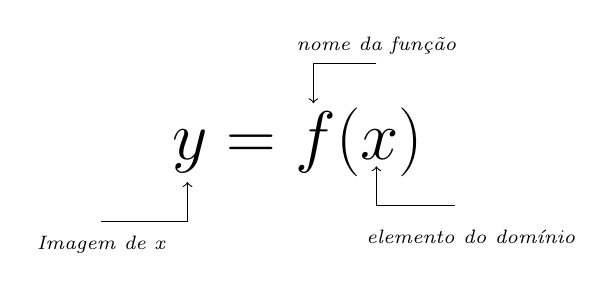
\begin{tikzpicture}
\draw(0,0) node {\Huge $y= f(x)$};
\draw[->](-2.5, -1)--(-1.4,-1)--(-1.4, -.5);
\draw(-2.5,-1.3) node {\em\scriptsize  Imagem de x};
\draw[->](1,1)--(.2,1)--(.2,.5);
\draw (1, 1)node[above]{\em \scriptsize nome da fun\c{c}\~ao};
\draw[->](2,-.8)--(1,-.8)--(1,-.3);
\draw (2.2,- 1.4)node[above]{\em \scriptsize elemento do dom\'{i}nio};
\end{tikzpicture}
\end{figure}

O conjunto \(A\) é chamado \index{domínio da função}domínio da função \(f\), o conjunto \(B\) é chamado \index{contradomínio}contradomínio de \(f\) e o subconjunto de \(B\) formado pelas imagens de todos os elementos de \(A\) é chamado \index{conjunto imagem}conjunto imagem da função \(f\).

\begin{figure}[H]
\centering


\begin{tikzpicture}
\begin{scope}[scale=.8]
\draw [rotate around={90.:(3.,3.5)},thin,fill=\currentcolor!80,fill opacity=0.1] (3.,3.5) ellipse (2.1 and 1.4);
\draw [rotate around={90.:(7.,3.5)},thin,fill=\currentcolor!80,fill opacity=0.1] (7.,3.5) ellipse (2.1 and 1.4);
\draw [line width=.5pt, rounded corners =10pt](5.3,1.2) rectangle(8.7,5.8) ;
\draw [latex-, shift={(5.,2.)},line width=.5pt]  plot[domain=0.8:2.4,variable=\t]({1.*2.8*cos(\t r)+0.*2.8*sin(\t r)},{0.*2.8*cos(\t r)+1.*2.8*sin(\t r)});
\draw(3,3.5) node { $x$};
\draw(7,3.5) node { $f(x)$};
\draw(4.7,5.2) node { $f$};
\draw(3,6) node { $A$};
\draw(7,6.2) node {$B$};
\end{scope}
\end{tikzpicture}
\end{figure}
De maneira geral, escreve-se:
\begin{equation*}
\begin{split}f:A \to B \\
x \mapsto f(x)\end{split}
\end{equation*}
Por exemplo, na {\hyperref[\detokenize{AF106-0:ativ-funcoes-pluviometria}]{Atividade: Pluviometria no Sistema Cantareira}}, se \(f\) é a função que associa a cada ano-mês o índice de chuva real naquele período, \(f(2014-3)=200\) nos informa que o índice de chuva real observada na região do sistema Cantareira no mês de março do ano de 2014 foi de \(200\) milímetros.

Em uma função \(f\) de \(A\) em \(B\), a dependência estabelecida entre as variáveis \(x \in A\) e \(y \in B\) permite que \(y\) seja identificada como “variável dependente” e \(x\) como  “variável independente”, uma vez que os valores assumidos por \(y\) são determinados em função da variação de \(x\) no domínio. Na atividade “Arranha-céu” por exemplo, a variável independente é aquela que representa os andares e a variável dependente é a altura do andar.

\begin{observation}{}

A definição de uma função \(f\) de \(A\) em \(B\) exige que a cada elemento \(x\in A\) corresponda uma imagem \(y=f(x)\in B\) e que não haja ambiguidade na determinação dessa imagem, ou seja, que ela seja única. Asssim, nem toda relação de \(A\) em {\color{red}\bfseries{}{}`}B é uma função. Por exemplo, a relação que associa a cada pessoa o número de seu telefone não é função, pois a imagem pode não ser única, ou seja, há ambiguidade: algumas pessoas têm mais de um número de telefone. E além disso, nem todas as pessoas têm telefone.
\end{observation}

\begin{reflection}{}

Junto com seus colegas, reflita sobre a definição que acabamos de ver. Vocês conseguem pensar em outros exemplos de relações do seu dia a dia que possam ser consideradas funções? Descrevam algumas delas e compartilhem com o restante da turma, destacando os conjuntos domínio e contradomínio dessas funções.
\end{reflection}
\newpage
\practice{}

\label{\detokenize{AF106-2:sec-funcao-organizando-ideias}}\label{\detokenize{AF106-2::doc}}\label{\detokenize{AF106-2:praticando}}


\begin{task}{ colorindo o mapa}
\label{\detokenize{AF106-2:atividade-colorindo-o-mapa}}\label{\detokenize{AF106-2:ativ-funcoes-colorindo-o-mapa}}


A imagem a seguir, que foi retirada do aplicativo Google Maps, exibe o trânsito na ponte Rio-Niterói e seus acessos em um determinado dia e hora. Várias informações podem ser observadas a partir dos elementos apresentados. Por exemplo, as cores nas vias informam a velocidade média dos veículos que trafegam por elas, conforme a legenda na parte inferior; a distância entre dois pontos quaisquer do mapa pode ser estimada usando a escala exibida no canto inferior direito. Gráficos como esse são produzidos a partir das relações entre diversas informações coletadas.

\begin{figure}[H]
\centering

\noindent\includegraphics[width=440bp]{{rio_niteroi_maps}.png}
\end{figure}

A tabela a seguir mostra os dados coletados sobre o tempo gasto pelos veículos (em média) para atravessar a ponte, ao longo de um dia.

\begin{table}[H]
\centering

\begin{tabu} to \textwidth{|c|c|>{\centering}m{.1\textwidth}|c|}
\hline
\thead
Período do Dia & Tempo (min) & Cor & Velocidade Média (km/min) \\
\hline
5:00 - 7:00 & 13 & & \\
\hline
7:00 - 9:00 & 18 & & \\
\hline
9:00 - 11:00 & 15 & & \\
\hline
11:00 - 13:00 & 15 & & \\
\hline
13:00 - 15:00 & 16 & & \\
\hline
15:00 - 17:00 & 16 & & \\
\hline
17:00 - 19:00 & 23 & & \\
\hline
19:00 - 21:00 & 14 & & \\
\hline
21:00 - 23:00 & 13 & & \\
\hline
\end{tabu}
\end{table}

\begin{enumerate}
\item {} 
Tomando como referência a ilustração anterior e utilizando a escala de cores a seguir, complete a terceira coluna da tabela com a cor que a ponte deveria estar colorida em cada período do dia destacado. Descreva os critérios que você utilizou na escolha de cada uma das cores e compare com os critérios dos seus colegas.
\begin{center}\begin{tikzpicture}[scale=3]
\tikzset{fontscale/.style = {font=\relsize{#1}}}
\fill[fill=green] (3.,1.) rectangle (3.6,1.2);
\fill[fill=orange] (3.65,1.) rectangle (4.25,1.2);
\fill[fill=red] (4.3,1.) rectangle (4.9,1.2);
\fill[fill=brown] (4.95,1.) rectangle (5.55,1.2);
\node[below left, font=\small] at (3,1.15) {RÁPIDO};
\node[below right, font=\small] at (5.55,1.15) {LENTO};
\node at ($(3,1)!0.5!(3.6,1.2)$) {verde};
\node at ($(3.65,1)!0.5!(4.25,1.2)$) {laranja};
\node at ($(4.3,1)!0.5!(4.9,1.2)$) {vermelho};
\node at ($(4.95,1)!0.5!(5.55,1.2)$) {marrom};
\end{tikzpicture}\end{center}
\item {} 
Você precisou associar uma mesma cor para para períodos diferentes do dia. Por que?

\item {} 
Sabendo que a ponte Rio-Niterói tem aproximadamente \(13\) km de extensão complete a quarta coluna da tabela com a velocidade média registrada em cada um dos períodos do dia.

\item {} 
É possível que uma mesma velocidade média esteja associada a dois tempos de travessia diferentes? Por quê?
\end{enumerate}
\end{task}

Na atividade anterior, observam-se diferentes relações entre os dados. Por exemplo, para cada tempo de travessia é possível associar uma única cor e uma única velocidade média. Da mesma maneira, a cada velocidade média está associada uma única cor e um único tempo de travessia. No entanto, a uma mesma cor é possível associar tempos diferentes e velocidades médias diferentes.

\begin{task}{ é função?}
\label{\detokenize{AF106-2:atividade-e-funcao}}\label{\detokenize{AF106-2:ativ-funcoes-e-funcao}}

No contexto da atividade anterior são observados diferentes conjuntos de dados: O conjunto dos tempos de travessia da ponte, \(A=\{13, 14, 15, 16, 18, 23\}\); O conjunto das cores que compoõem a escala, \(B=\{\) Verde, Laranja, Vermelho, Vinho \(\}\); e o conjunto de velocidades obtidas,{}`C{}`. Considere as diferentes relações de dependências estabelecidas entre esses conjuntos. Quais são funções?

\begin{table}[H]
\centering
\begin{tabu} to \textwidth{|c|c|>{\centering}m{6cm}|}
\hline
\thead
Relação & É função? &  Se não, por que? \\
\hline
De A em B
&&\\
\hline
De B em A
&&\\
\hline
De A em C
&&\\
\hline
De C em A
&&\\
\hline
De B em C
&&\\
\hline
De C em B
&&\\
\hline
\end{tabu}
\end{table}
\end{task}

Toda relação de um conjunto \(A\) em um conjunto \(B\) pode ser identificada por um conjunto de pares ordenados. Nesse caso, cada associação entre elementos do conjunto \(A\) e elementos do conjunto \(B\) fica representada por um par ordenado tal que o elemnto do conjunto \(A\) ocupa a primeira posição do par e o correspondente elemento do conjunto \(B\) a segunda posição.

Por exemplo, se consideramos a relação dos números reais em si mesmo que, a cada número real, associa o seu quadrado, os pares ordenados \((1,1), (2,4), (\sqrt{3},3), (-\pi,\pi^2)\) indicam elementos que estão relacinados. Já os pares ordenados \((9,5)\) e \((4,2)\), \((\sqrt{2},-2)\) formados por números reais, não indicam números associados pela mesma relação, uma vez que \(5\) não é quadrado de \(9\), \(2\) não é quadrado de \(4\) e \(-2\) não é o quadrado de \(\sqrt{2}\).

Como funções são um tipo especial de relação, a mesma ideia se estende para representação das funções. Assim, os pares ordenados de uma função \(f:A\to B\) serão da forma \((x,y)\) em que \(x\in A\) e \(y=f(x)\in B\).


\begin{task}{ não é função!}
\label{\detokenize{AF106-2:atividade-nao-e-funcao}}\label{\detokenize{AF106-2:ativ-funcoes-nao-e-funcao}}

Considere a relação formada por todos \((a,b)\) de números naturais tais que \(b\) é múltiplo de \(a\). Assim, \((2,4)\), \((2,6)\), \((3,6)\) e \((9, 9)\) são pares ordenado dessa relação, pois \(4\) é múltiplo de \(2\), \(6\) é múltiplo de \(2\) e de \(3\) e \(9\) é múltiplo de \(9\) . No entanto, \((4,2)\) e \((7,17)\) são pares ordenados de números naturais, mas não são pares dessa relação.
\begin{enumerate}
\item {} 
Exiba outros quatro pares ordenados dessa relação.

\item {} 
Explique porque essa relação não é uma função.

\item {} 
\((5, 405)\) é um par ordenado dessa relação. Quantos outros pares ordenados dessa relação têm 5 como primeiro elemento?

\item {} 
Dê exemplo de uma ou mais relações que não sejam funções. Não precisam ser exemplos numéricos.

\end{enumerate}
\end{task}

\begin{task}{ a família}
\label{\detokenize{AF106-2:atividade-a-familia}}

Cada ponto do gráfico a seguir representa uma das seguintes pessoas.

\begin{enumerate}
\item {} 
Associe cada ponto do gráfico à pessoa correspondente.

\item {} 
A relação expressa pelos pares ordenados (idade, altura) apresentados no gráfico é função? Por que?
\end{enumerate}


\begin{center}\begin{tikzpicture}[scale=1.4]
\draw[->](-0,0)--(6,0);
\draw(5.7,0) node [below]{idade};
\draw[->](0,-0)--(0,4);
\draw(0,3.95) node [above left, rotate =90]{altura};
\draw[fill](5.5,1.5) circle(1pt) node[right]{$F$};
\draw[dotted] (5.5,0)--(5.5,1.5)--(0,1.5);
\draw[fill](4.5,3.5) circle(1pt) node[above]{$E$};
\draw[dotted](4.5,0)--(4.5,3.5)--(0,3.5);
\draw[fill](3,3.5) circle(1pt) node[above]{$D$};
\draw[dotted](3,0)--(3,3.5);
\draw[fill](3,2.5) circle(1pt) node[right]{$C$};
\draw[dotted](3,2.5)--(0,2.5);
\draw[fill](2,1) circle(1pt) node[right]{$B$};
\draw[dotted](2,0) -- (2,1) --(0,1);
\draw[fill](.5,.3) circle(1pt) node[right]{$A$};
\draw[dotted](.5,0)--(.5,.3)--(0,.3);
\end{tikzpicture}\end{center}

\begin{figure}[H]
\centering



\noindent\includegraphics[width=300bp]{{familia}.png}
\label{\detokenize{AF106-2:fig-altura-idade}}\end{figure}


{\color{red}\bfseries{}*}Adaptado de The Language of Functions and Graphs, Shell Centre for Mathematical Education Publications Ltd., 1985.
\end{task}

Quando nos deparamos com uma função é fundamental identificarmos os conjuntos domínio e contradomínio, e a maneira como os elementos desses conjuntos estão relacionados. Tal maneira pode ser muito variada, no entanto, principalmente quando os conjuntos envolvidos são numéricos, é comum considerar como contradomínio o conjunto \(\mathbb{R}\). Por isso, daqui por diante, quando estivermos considerando funções numéricas, o contradomínio será igual a \(\mathbb{R}\).

Em muitos casos, a forma de associação entre os elementos é dada por uma expressão analítica. Vejamos alguns exemplos.

\((I)\) Para calcular o perímetro de um quadrado de lado \(\ell\) usa-se a expressão \(P=4\ell\). Percebe-se então que o perímetro está relacionado com o lado. A partir daí pode-se definir a função perímetro:
\begin{equation*}
\begin{split}P: ]0,+\infty[\to \mathbb{R} \quad ; \quad P(\ell)=4\ell.\end{split}
\end{equation*}
Da mesma forma a área de um quadrado de lado \(\ell\) é dada por \(A=\ell^2\), que permite definir a função:
\begin{equation*}
\begin{split}A: ]0,+\infty[\to \mathbb{R} \quad ; \quad A(\ell)=\ell^2.\end{split}
\end{equation*}
A variável \(\ell\) pode assumir qualquer valor dentro do intervalo \(]0,+\infty[\) que é o domínio da função \(P\) . Se quisermos saber o valor do perímetro do quadrado de lado 5cm, basta substituirmos \(\ell\) por 5 na expressão de  \(P(\ell)\). Ficamos assim com
\begin{equation*}
\begin{split}P(\textbf{5})=4\times \textbf{5} = 20\mathrm{cm}.\end{split}
\end{equation*}
A área do quadrado de lado 9cm é
\begin{equation*}
\begin{split}A(\textbf{9})=\textbf{9}^2=81cm^2.\end{split}
\end{equation*}
\((II)\) A fórmula de Lorentz já foi muito utilizada pelos médicos para o cálculo do “peso ideal” \(p\), em kg, em função da altura \(h\), em centímetros, do paciente.
\begin{equation*}
\begin{split}p:]0,300[\to \mathbb{R}\quad ; \quad p(h)=h-100-\dfrac{h-150}{k}\end{split}
\end{equation*}
em que \(k\) vale 4 para homens e vale 2 para mulheres.

Que tal usar a fórmula acima para calcular o seu peso ideal?

\((III)\) Imagine que um objeto é solto, a partir do repouso, de uma altura de \(10\) metros e percorre uma trajetória vertical em queda livre. Da Física, sabemos que sua altura \(h\) em metros medida a partir do solo, em função do tempo \(t\) em segundos, quando desprezamos a resistência do ar, é dada por
\begin{equation*}
\begin{split}h:[0,+\infty[\to \mathbb{R}\quad ; \quad h(t)=10-\dfrac{gt^2}{2},\end{split}
\end{equation*}
em que \(g\) representa a aceleração da gravidade em \(m/s^2\).metros por segundo ao quadrado.

Fazer a variável tempo assumir o valor \(t=0\) segundos na expressão de \(h(t)\) significa que estamos medindo a altura no início da contagem do tempo, ou seja a altura inicial do corpo. Nesse caso teremos
\begin{equation*}
\begin{split}h(\textbf{0})=10-\dfrac{g\ \textbf{0}^2}{2}=10.\end{split}
\end{equation*}
\emph{Se por exemplo, quisermos saber em quanto tempo o corpo chegará ao solo, o que devemos fazer?} Como a medição é feita a partir do solo, dizer que o objeto chegou ao solo é o mesmo que dizer que sua altura é igual a 0. Portanto, precisamos descobrir o valor da variável \(t\), de maneira que \(h(t)=0\). A partir da expressão de \(h(t)\) e aproximando \(g\) por \(10 m/s^2\), obtemos \(10-5t^2=0\), donde concluímos que  \(t=\sqrt{2}\) aproximadamente.


\begin{task}{ praticando a notação}
\label{\detokenize{AF106-2:atividade-praticando-a-notacao}}\label{\detokenize{AF106-2:ativ-praticando-notacao}}

Considere as funções \(f\), \(g\), \(k\) e \(h\), todas de domínio \(\mathbb{R}\), tais que:
\begin{equation*}
\begin{split}f(x)=3x^2+5x\quad ; \quad g(x)=\frac{x-1}{x^3+3}\quad ; \quad k(x)=(x-2)^2+6\quad ; \quad h(x)=2x-7\end{split}
\end{equation*}
Determine o valor de:


\begin{table}[H]
\centering
\begin{tabu} to \textwidth{|l|c|}
\hline
\thead
Função & Valor \\
\hline
\(f(3)\) & \\ 
\hline
\(g(-1)\) & \\
\hline
\(k(2)\) & \\
\hline
\(f(1)+g(1)\) & \\
\hline
\(g(2)-k(-1)\) & \\
\hline
\(k(0).f(-2)\) & \\
\hline
\(f(0)+h(0)-1\) & \\
\hline
\(f(-2).g(-2)+k(2)\) & \\
\hline
\(\dfrac{f(-3)}{k(0)}\) & \\
\hline
\(x\) quando \(h(x)=0\) & \\
\hline
\(x\) quando \(h(x)=3\) & \\
\hline
\end{tabu}
\end{table}

\end{task}

\begin{task}{ enchendo o cone}
\label{\detokenize{AF106-2:atividade-enchendo-o-cone}}\label{\detokenize{AF106-2:ativ-funcoes-enchendo-o-cone}}

O reservatório representado a seguir tem a forma de um cone cuja altura é \(6 m\) e a base é um círculo de raio \(3 m\). O volume \(V\) em litros de água no reservatório pode ser estimado a partir altura do nível da água \(h\) (em metros) de acordo com a seguinte expressão:
\begin{equation*}
\begin{split}V(h)=250h^3\end{split}
\end{equation*}\begin{center}\begin{tikzpicture}
\fill[thick,color=\currentcolor!80,fill=\currentcolor!80,fill opacity=0.10000000149011612, left color =white, right color =\currentcolor!80] (1.,0.) -- (-0.5,3.) -- (2.5,3.) -- cycle;
\draw [rotate around={-180:(1.0047836744699097,3.1435102340973167)},thick,left color=\currentcolor!80, right color=\currentcolor!80, middle color=white] (1.0047836744699097,3.1435102340973167) ellipse (1.5611029721362464cm and 0.5184113668542463cm);
\draw [rotate around={-180:(1.0071755117048646,4.715265351145975)},thick, left color=gray!80, right color=gray!60, middle color=white] (1.0071755117048646,4.715265351145975) ellipse (2.341654458204363cm and 0.7776170502813675cm);
\draw [thick] (1.,0.)-- (-1.3303743315507686,4.660748663101537);
\draw [thick] (1.,0.)-- (3.347109515260305,4.69421903052061);
\draw[dashed](1,0) -- (3.4,0);
\draw[|-|, dashed](2.6,0)--(2.6,3);
\draw (2.7,1.6) node[right] {$h$};
\draw[|-|, dashed](3.4,0)--(3.4,4.6);
\draw (3.5,2) node[right] {6 m};
\end{tikzpicture}\end{center}\begin{enumerate}
\item {} 
Determine \(V(2), V(3)\) e \(V(4)\) e explique os seus significados no contexto.

\item {} 
Quais os volumes de água, mínimo e máximo, que o reservatório comporta?

\item {} 
A que altura do nível da água corresponde o volume igual a \(3 456\) litros?

\end{enumerate}
\end{task}

\begin{task}{ uniformemente variado}
\label{\detokenize{AF106-2:atividade-uniformemente-variado}}\label{\detokenize{AF106-2:ativ-funcoes-uniformemente-variado}}

A posição \(S\) (em quilômetros), medida a partir de um referencial, de um veículo que se desloca segundo um movimento retilíneo uniformemente variado (MRUV) é dada em função do tempo \(t\) (medido em horas) pela seguinte expressão:
\begin{equation*}
\begin{split}S(t)=2t^2-4t+2\end{split}
\end{equation*}\begin{enumerate}
\item {} 
Determine a posição inicial do veículo. Explique o significado desse resultado a partir do contexto.

\item {} 
Após quanto tempo o veículo estará a 18km da origem?

\end{enumerate}
\end{task}

\know{}
\label{\detokenize{AF106-3::doc}}\label{\detokenize{AF106-3:sec-aprofundando}}\label{\detokenize{AF106-3:para-saber-mais}}

\begin{task}{ por que não é função?}
\label{\detokenize{AF106-3:ativ-nao-funcao}}\label{\detokenize{AF106-3:atividade-por-que-nao-e-funcao}}

Vimos que para que uma relação de \(A\) em \(B\) seja uma função não pode haver:

\((I)\) Elementos no conjunto \(A\) sem correspondente em \(B\);
\((II)\) Ambiguidade na determinação de correspondente em \(B\).

Determine se cada uma das relações apresentadas a seguir é função. Justifique suas respostas a partir das condições \((I)\) e \((II)\).
\begin{enumerate}
\item {} 
Seja \(\mathcal{P}\) o conjunto de todas as pessoas e considere a relação de \(\mathcal{P}\) em \(\mathcal{P}\), que a cada “pessoa” associa “irmão da pessoa”.

\item {} 
Seja \(\mathbb{R}\)  o conjunto dos números reais e considere a relação de \(\mathbb{R}\) em \(\mathbb{R}\), que a cada “número real \(x\) ” associa “raiz quadrada do número real \(x\) “.

\item {} 
Sejam \(\mathbb{R}^+\) o conjunto dos números reais positivos e \(\mathcal{T}\) o conjunto de todos os triângulos. Considere a relação de \(\mathbb{R}^+\) em \(\mathcal{T}\) que a cada “número real positivo \(x\) ” associa “triângulo de área \(x\) “.

\end{enumerate}

\end{task}

\begin{task}{ domínio e imagem}
\label{\detokenize{AF106-3:ativ-qual-e-imagem}}\label{\detokenize{AF106-3:atividade-dominio-e-imagem}}

Considere a seguinte lista de expressões algébricas.
\begin{multicols}{3}
\begin{enumerate}
\item {} 
\(f(x)=\sqrt{x}\)

\item {} 
\(G(z)=\sqrt{z-5}\)

\item {} 
\(h(s)=\frac{1}{3-s}\)

\item {} 
\(J(t)=\frac{1}{t+8}\)

\item {} 
\(T(x)=\frac{1}{\sqrt{x}}\)

\item {} 
\(R(x)=(x-2)^2+7\)

\item {} 
\(g(u)=5u^2+8\)

\item {} 
\(F(x)=(x+1)^2-3\)

\end{enumerate}
\end{multicols}

Veja que, em algumas das expressões, a variável independente não pode assumir alguns valores, por exemplo, na letra a) \(x\) não pode assumir valores negativos. Complete a tabela abaixo com o maior conjunto domínio possível que cada uma das funções pode ter e o correspondente conjunto imagem.


\begin{table}[H]
\centering
\begin{tabu} to \textwidth{|c|c|c|}
\hline
\thead
Expressão & Domínio $A$ & Imagem \\
\hline
\((a)\) & \(\mathbb{R}^+\) & \\
\hline
\((b)\) & & \\
\hline
\((c)\) & & \(\mathbb{R}\setminus \{0\}\) \\
\hline
\((d)\) & \(\mathbb{R}\setminus \{-8\}\) & \\
\hline
\((e)\) & & \\ 
\hline
\((f)\) & & \([7,+\infty[\) \\
\hline
\((g)\) & & \\
\hline
\((h)\) & & \\
\hline
\end{tabu}
\end{table}


\end{task}

\exercise
%\begin{multicols}{2}
\thispagestyle{empty}

\label{\detokenize{AF106-E1:sec-funcoes-exercicios}}\label{\detokenize{AF106-E1:exercicios}}\label{\detokenize{AF106-E1::doc}}

\begin{enumerate}
\item  Assim como os números triangulares (ver {\hyperref[\detokenize{AF106-4:ativ-funcoes-numeros-triangulares}]{Atividade: números triangulares no plano}}), fala-se nos números quadrados perfeitos, pentagonais, hexagonais, inspirados, respectivamente, pelas sequências abaixo.
\phantomsection\label{\detokenize{AF106-E1:fig-figurados}}
\begin{figure}[H]
\centering

\begin{tikzpicture}
\begin{scope}
\draw [fill=black] (0.,0.) circle (1.0pt);
\draw [fill=black] (0.5,0.) circle (1.0pt);
\draw [fill=black] (0.5,0.5) circle (1.0pt);
\draw [fill=black] (0.,0.5) circle (1.0pt);
\draw [fill=black] (1.5,0.) circle (1.0pt);
\draw [fill=black] (2.,0.) circle (1.0pt);
\draw [fill=black] (2.,0.5) circle (1.0pt);
\draw [fill=black] (1.5,0.5) circle (1.0pt);
\draw [fill=black] (2.5,0.) circle (1.0pt);
\draw [fill=black] (2.5,1.) circle (1.0pt);
\draw [fill=black] (1.5,1.) circle (1.0pt);
\draw [fill=black] (2.,1.) circle (1.0pt);
\draw [fill=black] (2.5,0.5) circle (1.0pt);
\draw [fill=black] (3.5,0.) circle (1.0pt);
\draw [fill=black] (4.,0.) circle (1.0pt);
\draw [fill=black] (4.,0.5) circle (1.0pt);
\draw [fill=black] (3.5,0.5) circle (1.0pt);
\draw [fill=black] (4.5,0.) circle (1.0pt);
\draw [fill=black] (4.5,1.) circle (1.0pt);
\draw [fill=black] (3.5,1.) circle (1.0pt);
\draw [fill=black] (5.,0.) circle (1.0pt);
\draw [fill=black] (5.,1.5) circle (1.0pt);
\draw [fill=black] (3.5,1.5) circle (1.0pt);
\draw [fill=black] (4.,1.) circle (1.0pt);
\draw [fill=black] (4.5,0.5) circle (1.0pt);
\draw [fill=black] (5.,0.5) circle (1.0pt);
\draw [fill=black] (5.,1.) circle (1.0pt);
\draw [fill=black] (4.5,1.5) circle (1.0pt);
\draw [fill=black] (4.,1.5) circle (1.0pt);
\draw [fill=black] (-1.,0.) circle (1.0pt);
\end{scope}
\end{tikzpicture}
\end{figure}
\begin{figure}[H]
\centering

\begin{tikzpicture}
\begin{scope}
\draw [fill=black] (-1.,0.) circle (1.0pt);
\draw [fill=black] (0.,0.) circle (1.0pt);
\draw [fill=black] (0.5,0.) circle (1.0pt);
\draw [fill=black] (0.6545084971874737,0.4755282581475766) circle (1.0pt);
\draw [fill=black] (0.25,0.7694208842938133) circle (1.0pt);
\draw [fill=black] (-0.15450849718747367,0.4755282581475768) circle (1.0pt);
\draw [fill=black] (2.,0.) circle (1.0pt);
\draw [fill=black] (2.5,0.) circle (1.0pt);
\draw [fill=black] (2.6545084971874737,0.4755282581475766) circle (1.0pt);
\draw [fill=black] (2.25,0.7694208842938133) circle (1.0pt);
\draw [fill=black] (1.8454915028125263,0.4755282581475768) circle (1.0pt);
\draw [fill=black] (3.,0.) circle (1.0pt);
\draw [fill=black] (3.3090169943749475,0.9510565162951532) circle (1.0pt);
\draw [fill=black] (2.5,1.5388417685876266) circle (1.0pt);
\draw [fill=black] (1.6909830056250525,0.9510565162951536) circle (1.0pt);
\draw [fill=black] (4.,0.) circle (1.0pt);
\draw [fill=black] (3.1545084971874737,0.4755282581475766) circle (1.0pt);
\draw [fill=black] (2.9045084971874737,1.2449491424413899) circle (1.0pt);
\draw [fill=black] (2.0954915028125263,1.24494914244139) circle (1.0pt);
\draw [fill=black] (4.5,0.) circle (1.0pt);
\draw [fill=black] (4.654508497187473,0.4755282581475766) circle (1.0pt);
\draw [fill=black] (4.25,0.7694208842938133) circle (1.0pt);
\draw [fill=black] (3.8454915028125263,0.4755282581475768) circle (1.0pt);
\draw [fill=black] (5.,0.) circle (1.0pt);
\draw [fill=black] (5.3090169943749475,0.9510565162951532) circle (1.0pt);
\draw [fill=black] (4.5,1.5388417685876266) circle (1.0pt);
\draw [fill=black] (3.6909830056250525,0.9510565162951536) circle (1.0pt);
\draw [fill=black] (5.154508497187473,0.4755282581475766) circle (1.0pt);
\draw [fill=black] (4.904508497187473,1.2449491424413899) circle (1.0pt);
\draw [fill=black] (4.095491502812527,1.24494914244139) circle (1.0pt);
\draw [fill=black] (5.5,0.) circle (1.0pt);
\draw [fill=black] (5.963525491562422,1.42658477444273) circle (1.0pt);
\draw [fill=black] (4.75,2.3082626528814396) circle (1.0pt);
\draw [fill=black] (3.5364745084375793,1.4265847744427305) circle (1.0pt);
\draw [fill=black] (5.654508497187474,0.4755282581475767) circle (1.0pt);
\draw [fill=black] (5.837430563354646,0.9408663263400823) circle (1.0pt);
\draw [fill=black] (5.557545365872711,1.7215466012812657) circle (1.0pt);
\draw [fill=black] (5.174750541804863,2.046031522986149) circle (1.0pt);
\draw [fill=black] (4.3461569097741055,2.014853473191221) circle (1.0pt);
\draw [fill=black] (3.942313819548215,1.7214442935010055) circle (1.0pt);
\end{scope}
\end{tikzpicture}
\end{figure}

\begin{figure}[H]
\centering

\begin{tikzpicture}
\begin{scope}
\draw [fill=black] (-1.,0.) circle (1.0pt);\draw [fill=black] (0.,0.) circle (1.0pt);\draw [fill=black] (-0.5,0.) circle (1.0pt);\draw [fill=black] (0.25,0.43301270189221935) circle (1.0pt);\draw [fill=black] (0.,0.8660254037844388) circle (1.0pt);\draw [fill=black] (-0.5,0.8660254037844389) circle (1.0pt);\draw [fill=black] (-0.75,0.43301270189221974) circle (1.0pt);\draw [fill=black] (1.,0.) circle (1.0pt);\draw [fill=black] (1.5,0.) circle (1.0pt);\draw [fill=black] (2.,0.) circle (1.0pt);\draw [fill=black] (2.5,0.8660254037844387) circle (1.0pt);\draw [fill=black] (2.,1.7320508075688776) circle (1.0pt);\draw [fill=black] (1.,1.7320508075688779) circle (1.0pt);\draw [fill=black] (0.5,0.8660254037844395) circle (1.0pt);\draw [fill=black] (1.75,0.43301270189221935) circle (1.0pt);\draw [fill=black] (1.5,0.8660254037844388) circle (1.0pt);\draw [fill=black] (1.,0.8660254037844389) circle (1.0pt);\draw [fill=black] (0.75,0.43301270189221974) circle (1.0pt);\draw [fill=black] (2.25,0.43301270189221935) circle (1.0pt);\draw [fill=black] (2.25,1.2990381056766582) circle(1.0pt);\draw [fill=black] (1.5,1.7320508075688776) circle (1.0pt);\draw [fill=black] (0.75,1.2990381056766587) circle (1.0pt);\draw [fill=black] (3.5,0.) circle (1.0pt);\draw[fill=black] (4.,0.) circle (1.0pt);\draw [fill=black] (4.5,0.) circle (1.0pt);\draw [fill=black] (5.,0.) circle (1.0pt);\draw [fill=black] (5.75,1.299038105676658) circle (1.0pt);\draw[fill=black] (5.,2.5980762113533165) circle (1.0pt);\draw [fill=black] (3.5,2.598076211353317) circle (1.0pt);\draw [fill=black] (2.75,1.2990381056766593) circle (1.0pt);\draw [fill=black] (5.,0.8660254037844387) circle (1.0pt);\draw [fill=black] (4.5,1.7320508075688776) circle (1.0pt);\draw [fill=black] (3.5,1.7320508075688779) circle (1.0pt);\draw [fill=black] (3.,0.8660254037844395) circle (1.0pt);\draw [fill=black] (4.25,0.43301270189221935) circle (1.0pt);\draw [fill=black] (4.,0.8660254037844388) circle (1.0pt);\draw [fill=black] (3.5,0.8660254037844389) circle (1.0pt);\draw [fill=black] (3.25,0.43301270189221974) circle (1.0pt);\draw [fill=black] (3.25,1.2990381056766587) circle (1.0pt);\draw [fill=black] (4.,0.8660254037844388) circle (1.0pt);\draw [fill=black] (4.,1.7320508075688776) circle (1.0pt);\draw [fill=black] (4.75,1.2990381056766582) circle (1.0pt);\draw [fill=black] (4.75,0.43301270189221935) circle (1.0pt);\draw [fill=black] (5.25,0.4330127018922193) circle (1.0pt);\draw [fill=black] (5.5,0.8660254037844386) circle (1.0pt);\draw [fill=black] (5.5,1.7320508075688752) circle (1.0pt);\draw [fill=black] (5.25,2.1650635094610884) circle (1.0pt);\draw [fill=black] (4.5,2.5980762113533156) circle (1.0pt);\draw [fill=black] (4.,2.5980762113533156) circle (1.0pt);\draw [fill=black] (3.25,2.1650635094611155) circle (1.0pt);\draw [fill=black] (3.,1.7320508075689163) circle (1.0pt);
\end{scope}
\end{tikzpicture}
\end{figure}

\begin{enumerate}
\item {} 
Para cada uma destas sequências, represente as próximas duas figuras;

\item {} 
Escreva uma sequência de números que possa estar associada a cada sequência de figuras;

\item {} 
Descreva a regra de formação de cada uma dessas sequências de números.

\end{enumerate}

\item Observe as duas sequências que se seguem:
\begin{equation*}
\begin{split}1, 1, 2, 3, 5, 8, 13, \dots\end{split}
\end{equation*}\begin{equation*}
\begin{split}1000, 100, 10, \dots\end{split}
\end{equation*}\begin{enumerate}
\item {} 
Descreva, em palavras ou em linguagem simbólica, uma regra de formação que você percebe em cada uma das sequências apresentadas.

\item {} 
Baseado na regra que você identificou no item anterior, descubra qual é o 20º termo de cada uma das sequências anteriores.

\end{enumerate}

\item Cada prisma obtém-se empilhando cubos do mesmo tamanho, brancos e cinzas, segundo uma regra sugerida na figura.
\phantomsection\label{\detokenize{AF106-E1:fig-prismas}}

\begin{figure}[H]
\centering

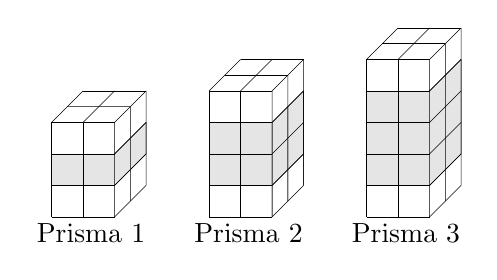
\begin{tikzpicture}[scale=2]
\fill[line width=2.pt,fill=black,fill opacity=0.10000000149011612] (0.,0.2) -- (0.400095,0.2) -- (0.6000712500000001,0.4) -- (0.6000475000000001,0.6) -- (0.4,0.4) -- (0.,0.4) -- cycle;
\draw[very thin] (0.,0.)-- (0.40019,0.);
\draw[very thin] (0.,0.4)-- (0.4,0.4);
\draw[very thin] (0.,0.6)-- (0.4,0.6);
\draw[very thin] (0.4,0.6)-- (0.6000237500000001,0.8);
\draw[very thin] (0.400095,0.2)-- (0.6000712500000001,0.4);
\draw[very thin] (0.4,0.4)-- (0.6000475000000001,0.6);
\draw[very thin] (0.400095,0.2)-- (0.,0.2);
\draw[very thin] (0.40019,0.)-- (0.600095,0.2);
\draw[very thin] (0.,0.6)-- (0.2,0.8);
\draw[very thin] (0.2,0.8)-- (0.6000237500000001,0.8);
\draw[very thin] (0.4,0.8)-- (0.2,0.6);
\draw[very thin] (0.1,0.7)-- (0.5000356207707869,0.7000237429513112);
\draw[very thin] (0.,0.)-- (0.,0.6);
\draw[very thin] (0.2,0.6)-- (0.2,0.);
\draw[very thin] (0.40019,0.)-- (0.4,0.6);
\draw[very thin] (0.6000237500000001,0.8)-- (0.600095,0.2);
\draw[very thin] (0.5001425,0.1)-- (0.5000356207707869,0.7000237429513112);
\draw[very thin] (0.,0.2)-- (0.400095,0.2);
\draw[very thin] (0.400095,0.2)-- (0.6000712500000001,0.4);
\draw[very thin] (0.6000712500000001,0.4)-- (0.6000475000000001,0.6);
\draw[very thin] (0.6000475000000001,0.6)-- (0.4,0.4);
\draw[very thin] (0.4,0.4)-- (0.,0.4);
\draw[very thin] (0.,0.4)-- (0.,0.2);
\draw(.25,-.1) node {Prisma 1};
\begin{scope}[xshift=1cm]
\fill[line width=2.pt,fill=black,fill opacity=0.10000000149011612] (0.,0.6) -- (0.,0.2) -- (0.400095,0.2) -- (0.6000712500000001,0.4) -- (0.6000237500000001,0.8) -- (0.4,0.6) -- cycle;
\draw[very thin] (0.600095,0.2)-- (0.6,1.);
\draw[very thin] (0.6,1.)-- (0.2,1.);
\draw[very thin] (0.,0.8)-- (0.,0.);
\draw[very thin] (0.,0.)-- (0.40019,0.);
\draw[very thin] (0.40019,0.)-- (0.4,0.8);
\draw[very thin] (0.4,0.8)-- (0.,0.8);
\draw[very thin] (0.,0.4)-- (0.4,0.4);
\draw[very thin] (0.2,0.8)-- (0.2,0.);
\draw[very thin] (0.,0.6)-- (0.4,0.6);
\draw[very thin] (0.4,0.6)-- (0.6000237500000001,0.8);
\draw[very thin] (0.5,0.9)-- (0.5001425,0.1);
\draw[very thin] (0.400095,0.2)-- (0.6000712500000001,0.4);
\draw[very thin] (0.4,0.4)-- (0.6000475000000001,0.6);
\draw[very thin] (0.400095,0.2)-- (0.,0.2);
\draw[very thin] (0.1,0.9)-- (0.5,0.9);
\draw[very thin] (0.2,0.8)-- (0.4,1.);
\draw[very thin] (0.40019,0.)-- (0.600095,0.2);
\draw[very thin] (0.4,0.8)-- (0.6,1.);
\draw[very thin] (0.,0.8)-- (0.2,1.);
\draw[very thin] (0.,0.)-- (0.,0.6);
\draw[very thin] (0.2,0.6)-- (0.2,0.);
\draw[very thin] (0.40019,0.)-- (0.4,0.6);
\draw[very thin] (0.6000237500000001,0.8)-- (0.600095,0.2);
\draw[very thin] (0.5001425,0.1)-- (0.5000356207707869,0.7000237429513112);
\draw[very thin] (0.,0.6)-- (0.,0.2);
\draw[very thin] (0.,0.2)-- (0.400095,0.2);
\draw[very thin] (0.400095,0.2)-- (0.6000712500000001,0.4);
\draw[very thin] (0.6000712500000001,0.4)-- (0.6000237500000001,0.8);
\draw[very thin] (0.6000237500000001,0.8)-- (0.4,0.6);
\draw[very thin] (0.4,0.6)-- (0.,0.6);
\draw(.25,-.1) node {Prisma 2};
\begin{scope}[xshift=1cm]
\fill[line width=2.pt,fill=black,fill opacity=0.10000000149011612] (0.,0.8) -- (0.4,0.8) -- (0.6,1.) -- (0.6000712500000001,0.4) -- (0.400095,0.2) -- (0.,0.2) -- cycle;
\draw[very thin] (0.,0.)-- (0.40019,0.);
\draw[very thin] (0.4,0.8)-- (0.,0.8);
\draw[very thin] (0.,0.4)-- (0.4,0.4);
\draw[very thin] (0.,0.6)-- (0.4,0.6);
\draw[very thin] (0.4,0.6)-- (0.6000237500000001,0.8);
\draw[very thin] (0.400095,0.2)-- (0.6000712500000001,0.4);
\draw[very thin] (0.4,0.4)-- (0.6000475000000001,0.6);
\draw[very thin] (0.400095,0.2)-- (0.,0.2);
\draw[very thin] (0.40019,0.)-- (0.600095,0.2);
\draw[very thin] (0.,1.)-- (0.2,1.2);
\draw[very thin] (0.,1.)-- (0.4,1.);
\draw[very thin] (0.4,1.)-- (0.6,1.2);
\draw[very thin] (0.2,1.)-- (0.4,1.2);
\draw[very thin] (0.2,1.2)-- (0.6,1.2);
\draw[very thin] (0.1,1.1)-- (0.5,1.1);
\draw[very thin] (0.,1.)-- (0.,0.);
\draw[very thin] (0.2,0.)-- (0.2,1.);
\draw[very thin] (0.4,1.)-- (0.40019,0.);
\draw[very thin] (0.5001425,0.1)-- (0.5,1.1);
\draw[very thin] (0.6,1.2)-- (0.600095,0.2);
\draw[very thin] (0.4,0.8)-- (0.6,1.);
\draw[very thin] (0.,0.8)-- (0.4,0.8);
\draw[very thin] (0.4,0.8)-- (0.6,1.);
\draw[very thin] (0.6,1.)-- (0.6000712500000001,0.4);
\draw[very thin] (0.6000712500000001,0.4)-- (0.400095,0.2);
\draw[very thin] (0.400095,0.2)-- (0.,0.2);
\draw[very thin] (0.,0.2)-- (0.,0.8);
\draw(.25,-.1) node{Prisma 3};
\end{scope}
\end{scope}
\end{tikzpicture}\end{figure}
\begin{enumerate}
\item {} 
Descreva, em palavras ou em linguagem simbólica, uma regra de formação sugerida pela figura.

\item {} 
Para construir o prisma \(4\) dessa sequência, segundo o padrão por você descrito, quantos cubos cinzas são necessários?

\item {} 
Justifique a afirmação: “O número total de cubos cinzas necessários para construir qualquer prisma desta sequência é par.”

\item {} 
Segundo o padrão por você descrito, quantos cubos cinzas terá o prisma 200?

\item {} 
Explicite uma expressão numérica que permita determinar o número de cubos cinzas do Prisma \(n\) em função de \(n\), isto é, uma expressão que de forma geral associe a ordem da figura à quantidade de cubos cinzas em sua composição.

\item {} 
Justifique novamente a afirmação do item (c), agora a partir da expressão que você explicitou no ítem anterior.

\item {} 
Se \(x\) representar o número total de cubos (brancos e cinzas) de um prisma desta sequência, qual das expressões seguintes representará o número de cubos cinzas desse prisma. Justifique sua escolha.

\end{enumerate}
\thispagestyle{empty}

\begin{equation*}
\begin{split}\square \ x-8 \quad \quad \square \ 2x-4 \quad \quad \square \ x-4 \quad \quad \square \ 4x\end{split}
\end{equation*}
\item  Ao final de um treino para a prova de 100 metros rasos, uma corredora recebe de seu treinador a seguinte tabela com as marcas intermediárias da sua melhor corrida.

Considerando que a velocidade da atleta é constante ao longo dos 100 metros responda as seguintes perguntas.
\begin{enumerate}
\item {} 
Quanto tempo ela gastou para percorrer os primeiros \(30\) metros?

\item {} 
Pensando em uma estratégia para melhorar a preformance da atleta, seu treinador resolve detalhar a tabela com os tempos correspondentes a cada \(10\) metros. Construa essa tabela.

\end{enumerate}

\item Hoje de manhã a Ana saiu de casa e dirigiu-se para a escola. Fez uma parte do percurso andando e a outra parte correndo. O gráfico a seguir mostra a distância percorrida pela Ana, em função do tempo que decorreu desde o instante em que ela saiu de casa até ao instante em que chegou à escola.
\begin{center}\begin{tikzpicture}
\draw [->](0,0)--(6.5,0);
\draw (6.3,0) node[above]{tempo};
\draw[->](0,0)--(0,4);
\draw (0,4) node [right]{dist\^{a}ncia};
\draw(0,0)--(1.5,2.7)--(5.5,3.5);
\draw[dashed](1.5,0)--(1.5,2.7)--(0,2.7);
\draw[dashed](5.5,0)--(5.5,3.5)--(0,3.5);
\draw(1.5,-.3) node {$t_1$};
\draw(5.5,-.3) node {$t_2$};
\draw(-.3,2.7) node {$d_1$};
\draw(-.3,3.5) node {$d_1$};
\end{tikzpicture}\end{center}
Apresentam-se, a seguir, quatro afirmações. De acordo com o gráfico, apenas uma é verdadeira. Assinale-a com X, explicando por que motivo cada uma das demais opções é falsa.

(    ) A Ana percorreu metade da distância andando e a outra metade correndo.

(    ) A Ana percorreu maior distância andando do que correndo.

(    ) A Ana esteve mais tempo correndo do que andando.

(    ) A Ana iniciou o percurso correndo e terminou-o andando.

\item Em Janeiro, o Vitor, depois de ter vindo do barbeiro, decidiu estudar o comprimento do seu cabelo, registando todos os meses a sua medida. O gráfico seguinte representa o crescimento do cabelo do Vitor, desde o mês de Janeiro (mês 0), até ao mês de Junho (mês 5).
\phantomsection\label{\detokenize{AF106-E1:fig-cabelo}}

\begin{center}
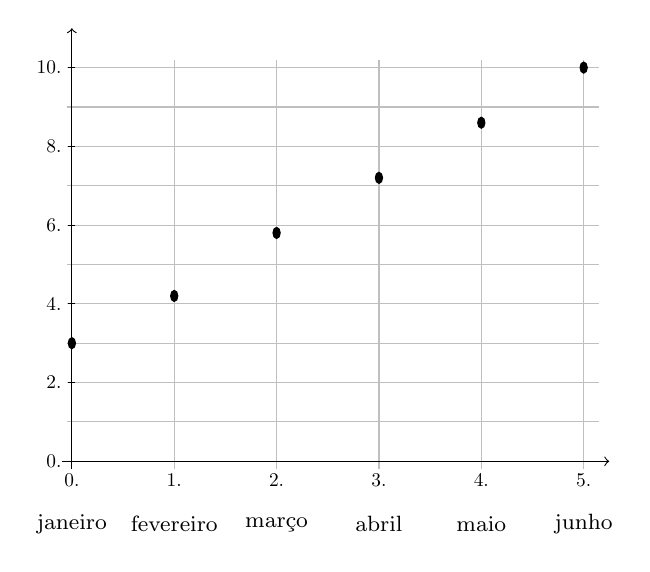
\begin{tikzpicture}[xscale=.65]
\draw [color=lightgray,, xstep=2.0cm,ystep=.5cm] (-.1,-.1) grid (10.3,5.1);
\draw[->,color=black] (-.2,0.) -- (10.5,0.);
\foreach \x in {0., 1.,2.,3.,4.,5.}
\draw[shift={(2*\x,0)},color=black] (0pt,-2pt) -- (0pt,-2pt) node[below, scale=.7] { $\x$};
\foreach \m[count=\x from 0]in {{janeiro} , {fevereiro} , {mar\c{c}o}, {abril}, {maio}, {junho}}
\draw (2*\x, -.8) node{\footnotesize \m};
\draw[->,color=black] (0.,-.1) -- (0.,5.5);
\foreach \y in {0., 2.,4.,6., 8., 10.}
\draw[shift={(0,.5*\y)},color=black] (2pt,0pt) -- (-2pt,0pt) node[left, scale=.7] { $\y$};
\draw [fill](0,1.5)circle (2pt);
\draw [fill](2,2.1)circle (2pt);
\draw [fill](4,2.9)circle (2pt);
\draw [fill](6,3.6)circle (2pt);
\draw [fill](8,4.3)circle (2pt);
\draw [fill](10,5)circle (2pt);
\end{tikzpicture}\end{center}\begin{enumerate}
\item {} 
A partir dos dados apresentados no gráfico, complete a tabela acima.

\item {} 
Em cada mês, quantos centímetros cresceu o cabelo do Vitor?

\item {} 
Escreva uma expressão geral que represente o Comprimento (C) do cabelo do Vitor, em função do número de meses (M) passados após o corte de cabelo inicial.

\item {} 
Considerando o comportamento indicado no gráfico, se o cabelo do Vitor crescer \(19,8 \ cm\), se que haja cortes no período, quantos meses terão se passado desde o último corte de cabelo? Justifique.

\end{enumerate}

\item Considere a função \(g:\mathbb{R}\to\mathbb{R}\quad\) tal que \(\quad g(x)=9-x^2\).
\begin{enumerate}
\item {} 
Coloque em ordem crescente os números \(g(\sqrt{2})\), \(g(\sqrt{5})\) e  \(g(\sqrt{10})\).

\item {} 
Determine todos os possíveis valores de \(x\) do domínio que têm imagem igual a 8.

\item {} 
Existe algum \(x\in \mathbb{R}\) cuja imagem é igual a 10? Por que?

\item {} 
Que condição deve satisfazer um número real \(b\) para que seja a imagem de algum número real \(x\), isto é, \(b=g(x)\) ?

\end{enumerate}

\item Considere o processo que associa \emph{cada número natural à soma de seus algarismos}.
\begin{enumerate}
\item {} 
Por meio do processo descrito acima o número natural \(13717\) será associado a que número?

\item {} 
Proponha um número cujo resultado do processo seja \(22\).

\item {} 
Quantos números entre \(1\) e \(10000\) nos levam ao resultado \(3\)?

\item {} 
É possível obter qualquer número natural como resultado desse processo? Explique.

\end{enumerate}
\end{enumerate}
%\end{multicols}

\explore{ gráfico}
\label{\detokenize{AF106-4:explorando-grafico}}\label{\detokenize{AF106-4::doc}}\label{\detokenize{AF106-4:sec-explorando-grafico}}
Segundo informações do \href{http://www.bigdatabusiness.com.br/visualizacao-de-dados-por-que-transformar-big-data-em-graficos/}{Big Data Business}, as palavras estimulam o lado esquerdo do cérebro e são um recurso essencial para a manutenção da memória. No entanto, as imagens são ainda mais eficazes, porque elas conseguem ativar os dois lados do cérebro simultaneamente e, assim, permitem o resgate de ideias e informações com maior precisão e agilidade. Especialmente quando se quer analisar grande quantidade de dados, apresentá-los em uma imagem ou em um gráfico, pode favorecer a comunicação.

\begin{figure}[H]
\centering
\capstart

\noindent\includegraphics[width=400bp]{{grafico-final}.png}
\caption{Alguns exemplos de representações gráficas}\label{\detokenize{AF106-4:id1}}\end{figure}

Representar graficamente conjuntos de dados e suas relações pode fazer toda a diferença para transmitir informações. Há vários tipos de gráficos, cada um tem a sua particularidade e serve para transmitir as informações de forma específica. Nesta seção iremos estudar a representação gráfica de funções.

Vamos considerar a seguinte situação:


\begin{task}{ ação promocional}
\label{\detokenize{AF106-4:atividade-acao-promocional}}

Uma empresa resolve lançar uma ação promocional na internet usando uma \href{https://pt.wikipedia.org/wiki/Hashtag}{hashtag}. Um mês após o lançamento, o presidente dessa empresa resolve analisar o impacto da ação na rede. Para isso ele pede a um de seus funcionários que prepare um relatório sobre o número de vezes que a \emph{hashtag} foi mencionada nas redes sociais em cada dia durante aquele mês. O funcionário resolveu apresentar os dados das seguintes duas formas:
\begin{figure}[H]
\centering

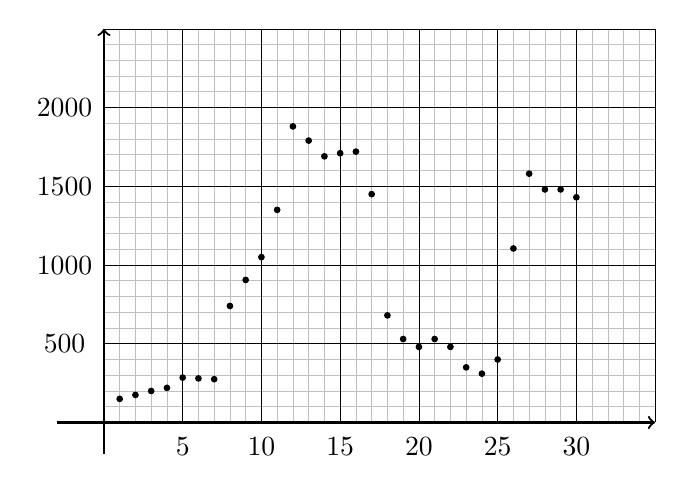
\begin{tikzpicture}
\tikzstyle{ponto}=[circle, minimum size=2pt, inner sep=0, draw=black, fill=black, shift only]
\draw[help lines,xstep=.2,ystep=.2, lightgray] (0,0) grid (7,5);
\draw[help lines, black, xstep=1, ystep=1] (0,0) grid (7,5);
\draw[thick,->](-.6,0)--(7,0);
\draw[thick,->](0,-.4)--(0,5);
\foreach \x in {5, 10, ..., 30}
\draw(.2*\x,-.3)node{\x};
\foreach \y in {500, 1000, 1500, 2000}
\draw(-.5, .002*\y)node{\y};
\node [ponto] at (.2,.3){};
\node [ponto] at (.4,.35){};\node [ponto] at (.6,.4){};\node [ponto] at (.8,.44){};   \node [ponto] at (1,.57){};\node [ponto] at (1.2,.56){};\node [ponto] at (1.4,.55){};\node [ponto] at (1.6,1.48){};\node [ponto] at (1.8,1.81){};\node [ponto] at (2,2.1){};\node [ponto] at (2.2,2.7){};\node [ponto] at (2.4,3.76){};\node [ponto] at (2.6,3.58){};\node [ponto] at (2.8,3.38){};\node [ponto] at (3,3.42){};\node [ponto] at (3.2,3.44){};\node [ponto] at (3.4,2.9){};\node [ponto] at (3.6,1.36){};\node [ponto] at (3.8,1.06){};\node [ponto] at (4,.96){};\node [ponto] at (4.2,1.06){};\node [ponto] at (4.4,.96){};\node [ponto] at (4.6,.7){};\node [ponto] at (4.8,.62){};\node [ponto] at (5.,.8){};\node [ponto] at (5.2,2.21){};\node [ponto] at (5.4,3.16){};\node [ponto] at (5.6,2.96){};;  \node [ponto] at (5.8,2.96){};;\node [ponto] at (6,2.86){};
\end{tikzpicture}
\end{figure}
\begin{enumerate}
\item {} 
Quantas vezes a \emph{hashtag} foi mencionada mais de 1500 vezes em um dia?

\item {} 
Em que dia a \emph{hashtag} foi mais citada?

\item {} 
Identifique todos os períodos em que houve crescimento no número de citações.

\item {} 
Faça o mesmo para o decrescimento.

\item {} 
Escreva um parágrafo explicando o comportamento global do gráfico, apontando possíveis causas para as variações observadas.

\end{enumerate}

\end{task}

Uma função, essencialmente, relaciona duas ou mais grandezas ou variáveis, de forma que são obtidos pares \((x,y)\), em que \(x\) pertence ao domínio da função e \(y=f(x)\). Perceba que a ordem em que os termos que compõem o par são apresentados é importante. Em matemática, chamamos esse tipo de objeto de \emph{par ordenado}, eles são objetos fundamentais para a compreensão do gráfico de uma função.

No caso de funções reais de variável real, isto é, cujos domínio e contradomínio são o conjunto dos números reais (ou subconjuntos dele) tanto \(x\) como \(y\) serão números reais.

A representação geométrica mais comum para esses pontos, e que você provavelmente já conhece, é no \index{plano cartesiano}plano cartesiano. Essa representação tem como base duas retas numéricas perpendiculares que se intersectam em suas origens conforme a figura abaixo.

\begin{center}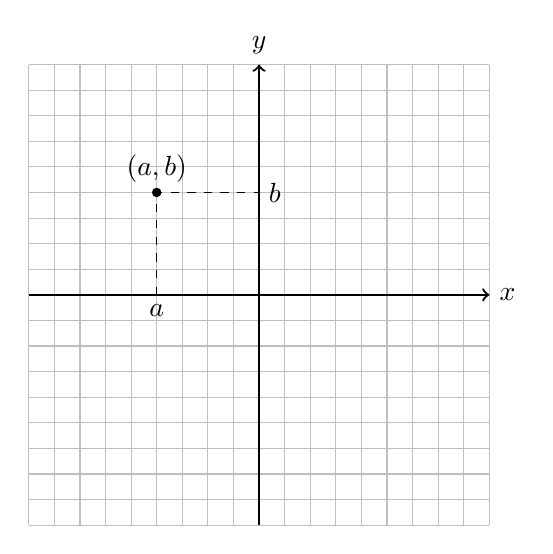
\begin{tikzpicture}[scale=.65]
\tikzstyle{ponto}=[circle, minimum size=3pt, inner sep=0, draw=black, fill=black, shift only]
\draw[lightgray](-4.5,-4.5)grid[xstep=.5,ystep=.5,line width =1pt](4.5,4.5);
\draw[->,thick](-4.5,0)--(4.5,0) node[right]{$x$};
\draw[->,thick](0,-4.5)--(0,4.5)node[above]{$y$};
\draw[dashed](-2,0)--(-2,2)--(0,2);
\node[ponto] at (-2,2){};
\node[above] at (-2,2){$(a,b)$};
\node[below] at (-2,0){$a$};
\node[right] at (0,2){$b$};
\end{tikzpicture}\end{center}

As retas que compõem um sistema cartesiano são chamadas de \index{eixos coordenados}eixos do plano cartesiano. O eixo em que são registradas as primeiras coordenadas do par é chamado de \index{eixo das abscissas}eixo das abscissas. O outro eixo, em que são registradas as segundas coordenadas do par é chamado de \index{eixo das ordenadas}eixo das ordenadas.

Já vimos alguns exemplos de funções em atividades anteriores, vamos explorá-los um pouco mais.


\begin{task}{ do mapa para o gráfico}
\label{\detokenize{AF106-4:ativ-funcoes-do-mapa-para-grafico}}\label{\detokenize{AF106-4:atividade-do-mapa-para-o-grafico}}

\begin{enumerate}
\item {} 
A partir das colunas \emph{Tempo de travessia} e \emph{Cor} da {\hyperref[\detokenize{AF106-2:ativ-funcoes-colorindo-o-mapa}]{Atividade: colorindo o mapa}}, escreva o conjunto de pares ordenados da forma (tempo, cor) respeitando o critério que você escolheu para a determinação das cores.

\item {} 
Represente graficamente este conjunto de pares ordenados.

\item {} 
Para colorir as vias de todo o mapa, precisamos distribuir as cores para outros valores de tempo. Como você faria a distribuição para o intervalo de \(0\) a \(25\) minutos considerando um trecho qualquer de \(13\) km (a mesma extensão da ponte)?

\item {} 
Encontre outra maneira de representar graficamente a associação entre os tempos e as cores.

\end{enumerate}

\end{task}

\begin{task}{ números triangulares no plano}
\label{\detokenize{AF106-4:atividade-numeros-triangulares-no-plano}}\label{\detokenize{AF106-4:ativ-funcoes-numeros-triangulares}}

Represente, no plano cartesiano, o conjunto de pontos que correspondem aos pares ordenados \(\{(n,T_n)\ ;\ n\in\{1,2,...,8\}\}\), em que \(T_n\) é o \(n\)-ésimo número triangular.

\end{task}

\begin{task}{ jornada até a escola}
\label{\detokenize{AF106-4:atividade-jornada-ate-a-escola}}\label{\detokenize{AF106-4:ativ-funcoes-jornada-ate-a-escola}}

Leonardo mora a \(6\) km da escola onde estuda e utiliza o transporte escolar, que o busca na porta de sua casa. Em um certo dia, o percurso de Leonardo até sua escola foi assim: Ele estava na porta de casa às \(7\) horas, como de costume, mas o transporte escolar atrasou, passando em sua casa somente às \(7h05min\). Leonardo entrou na van e sentou no penúltimo lugar vago. Ainda faltava Marina. “Ela mora a \(3\) km da minha casa!”, lembrou Leonardo. Às \(7h10min\) em ponto, o transporte escolar chegou à casa de Marina, que já estava pronta aguardando para embarcar. Para tentar compensar o atraso, o motorista resolveu tomar um atalho, mas a estratégia não funcionou. Às \(7h15min\) precisou ficar parado por \(5\) minutos em frente a uma cancela aguardando um trem de carga passar. Finalmente, às \(7h25min\) chegaram à escola, \(5\) minutos antes do sinal tocar.

No plano cartesiano a seguir, o eixo horizontal indica o tempo em minutos e o eixo vertical a distância percorrida em quilômetros. Os pontos marcados correspondem às distâncias percorridas por diversos estudantes da escola a cada \(5\) minutos no período das \(7h\) às \(7h30min\) da mesma manhã descrita na situação acima.

\phantomsection\label{\detokenize{AF106-4:fig-pontos-jornada}}
\begin{figure}[H]
\centering

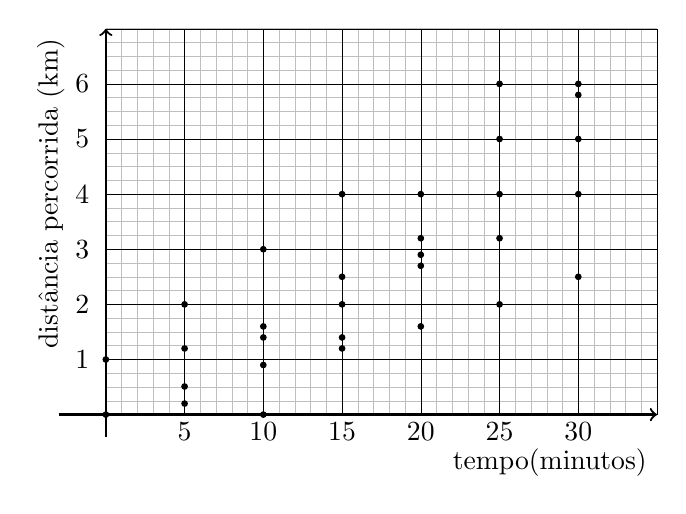
\begin{tikzpicture}
\tikzstyle{ponto}=[circle, minimum size=2pt, inner sep=0, draw=black, fill=black, shift only]
\begin{scope}[yscale=.7]
\draw[help lines,xstep=.2,ystep=.25, lightgray] (0,0) grid (7,7);
\draw[help lines, black, xstep=1, ystep=1] (0,0) grid (7,7);
\draw[thick,->](-.6,0)--(7,0) node[below left, yshift =-.3cm]{tempo(minutos)};
\draw[thick,->](0,-.4)--(0,7) node[rotate=90,left,yshift =.7cm]{ distância percorrida (km)};
\foreach \x in {5, 10, ..., 30}
\draw(.2*\x,-.3)node{\x};
\foreach \y in {1, 2, 3, 4, 5, 6}
\draw(-.3, \y)node{\y};
\node[ponto] at(0,0){};\node[ponto] at(0,1){};\node[ponto] at(1,.2){};\node[ponto] at(1,.51){};\node[ponto] at(1,1.2){};\node[ponto] at(1,2){};\node[ponto] at(2,0){};\node[ponto] at(2,0.9){};\node[ponto] at(2,1.4){};\node[ponto] at(2,1.6){};\node[ponto] at(2,3){};\node[ponto] at(3,1.2){};\node[ponto] at(3,2.5){};\node[ponto] at(3,1.4){};\node[ponto] at(3,2){};\node[ponto] at(3,4){};\node[ponto] at(4,1.6){};\node[ponto] at(4,2.7){};\node[ponto] at(4,2.9){};\node[ponto] at(4,3.2){};\node[ponto] at(4,4){};\node[ponto] at(5,2){};\node[ponto] at(5,3.2){};\node[ponto] at(5,4){};\node[ponto] at(5,5){};\node[ponto] at(5,6){};\node[ponto] at(6,2.5){};\node[ponto] at(6,4){}; \node[ponto] at(6,5){};\node[ponto] at(6,5.8){};\node[ponto] at(6,6){};
\end{scope}
\end{tikzpicture}
\end{figure}


\begin{enumerate}
\item {} 
Conecte os pontos que correspondem à jornada de Leonardo, desde a porta da sua casa até a chegada à escola, no dia descrito acima.

\item {} 
Faça uma estimativa da distância a que Leonardo estará de sua casa às \(7h07min\).

\item {} 
Escolha um conjunto de pontos que possa representar a jornada de um outro estudante da sua casa à escola e descreva essa jornada.

\end{enumerate}
\end{task}

\arrange{ gráficos}
\label{\detokenize{AF106-5:sec-organizando-graficos}}\label{\detokenize{AF106-5:organizando-as-ideias-graficos}}\label{\detokenize{AF106-5::doc}}
É hora de organizar as ideias sobre representação gráfica de uma função. Vimos que, para representar graficamente as funções, os pares ordenados são fundamentais. Cada par identifica as grandezas ou variáveis relacionadas e a ordem no par distingue o papel de cada uma delas: elemento do domínio, abscissa, e imagem, ordenada. Sendo assim, a representação gráfica de uma função exige: a identificação das variáveis do problema e a identificação da relação estabelecida entre as variáveis.

Para funções reais de variável real, isto é, funções cujo domínio é um subconjunto de \(\mathbb{R}\) e o contradomínio é \(\mathbb{R}\), sua representação gráfica no plano cartesiano será o conjunto dos pares ordenados \((x,f(x))\) em que \(x\) pertence ao domínio da função.

\begin{figure}[H]
\centering

\begin{tikzpicture}[scale=1.5]
\draw[line width=1.pt,color=\currentcolor!80,samples=100,domain=-2.05:1.8] plot(\x,{.5*sin((3.5*(\x)-3.2)*180/pi)-0.6*cos((4.5*(\x)+2.0)*180/pi)});
\draw[->](-.8,-1)--(-.8,1.5) ;
\draw[->](-2.3,0)--(2.5,0);
\draw[fill](.965,-.5)circle(1pt);
\draw[dashed](-.8,-.5)--(.965,-.5);
\draw[dashed](.965,-.5)--(.965,-0);
\draw(.965,-0)node[scale=.5, above]{$x$};
\draw[dashed](-.8,-.5)node[left]{$f(x)$};
\draw(.97,-.55) node[right] {($x, f(x)$)};
\end{tikzpicture}
\end{figure}

\begin{reflection}{}

Os conjuntos domínio e imagem ficam evidenciados na representação gráfica de uma  função a partir dos eixos coordenados. Observe a representação gráfica a seguir, em que estão destacados conjuntos sobre os eixos. Qual deles você identifica como domínio? A que conjunto corresponde o outro?
\begin{figure}[H]
\centering

\begin{tikzpicture}[scale=1.5]
\draw[line width=1.pt,color=\currentcolor!80,samples=100,domain=-1.5:1.8] plot(\x,{.5*sin((3.5*(\x)-3.2)*180/pi)-0.6*cos((4.5*(\x)+2.0)*180/pi)});
\draw[->](-.8,-1)--(-.8,2) ;
\draw[->](-2,0)--(2.5,0);
\draw[dashed](-2,.95)--(2.5,.95);
\draw[dashed](-2,-.67)--(2.5,-.67);
\draw[color=red, thick](-.8, -.67)--(-.8, .95);
\begin{scope}[xshift=5cm]
\draw[line width=1.pt,color=\currentcolor!80,samples=100,domain=-1.5:1.8] plot(\x,{.5*sin((3.5*(\x)-3.2)*180/pi)-0.6*cos((4.5*(\x)+2.0)*180/pi)});
\draw[->](-.8,-1)--(-.8,2) ;
\draw[->](-2,0)--(2.5,0);
\draw[dashed](-1.5,-1)--(-1.5,2);
\draw[dashed](1.8,-1)--(1.8,2);
\draw[color=blue, thick](-1.5,0)--(1.8,0);
\end{scope}
\end{tikzpicture}\
\end{figure}
\end{reflection}


\practice{}

%\label{\detokenize{AF106-5:sec-praticando-grafico}}\label{\detokenize{AF106-5:praticando}}

\begin{task}{ Indo para escola*}
\label{\detokenize{AF106-5:ativ-indo-para-escola}}\label{\detokenize{AF106-5:atividade-indo-para-escola}}

Arthur, Caetano, Gael, Levi e Pedro utilizam a mesma avenida para ir à escola a cada manhã. Levi vai com seu pai de carro, Arthur de bicicleta e Gael caminhando. Os demais variam, a cada dia, a forma como percorrem o trajeto. O mapa a seguir mostra a posição da casa de cada um em relação à escola.
\phantomsection\label{\detokenize{AF106-5:fig-mapa-escola}}

\begin{figure}[H]
\centering

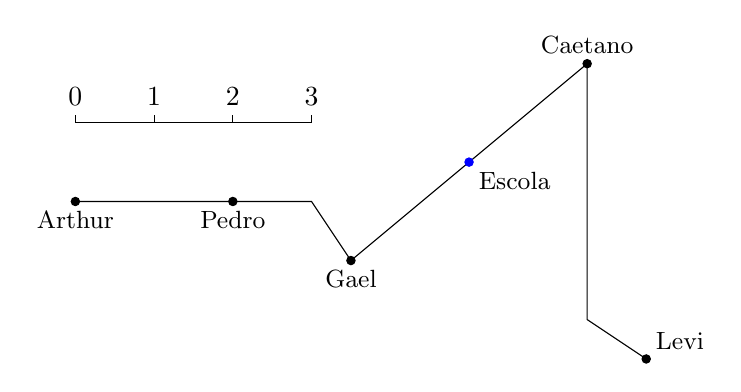
\begin{tikzpicture}
\tikzstyle{ponto}=[circle, minimum size=3pt, inner sep=0, draw=black, fill=black, shift only]
\draw(-2,2)grid(1,2.1);
\foreach \x in {0,1,2,3}
\node at (\x - 2,2.1)[above]{\x};
\coordinate (A) at (-2,1);
\coordinate (B) at (0,1);
\coordinate (C) at (1,1);
\coordinate (D) at (1.5,.25);
\coordinate (E) at (3,1.5);
\coordinate (F) at (4.5,2.75);
\coordinate (G) at (4.5,-.5);
\coordinate (H) at (5.25,-1);
\draw(A)--(B)--(C)--(D)--(E)--(F)--(G)--(H);
\node[ponto] at (A){};\node[ponto] at (B){};\node[ponto] at (D){};\node[ponto, blue] at (E){};\node[ponto] at (F){};\node[ponto] at (H){};
\node[below] at (A){\small Arthur};\node[below] at (B){\small Pedro };\node[below] at (D){\small Gael};\node[below right] at (E){\small Escola};\node[above] at (F){\small Caetano};\node[above right] at (H){\small Levi};
\end{tikzpicture}
\end{figure}

Os pontos marcados no plano cartesiano abaixo fornecem informações sobre a jornada de cada criança na última segunda-feira.
\phantomsection\label{\detokenize{AF106-5:fig-grafico-jornada}}

\begin{figure}[H]
\centering

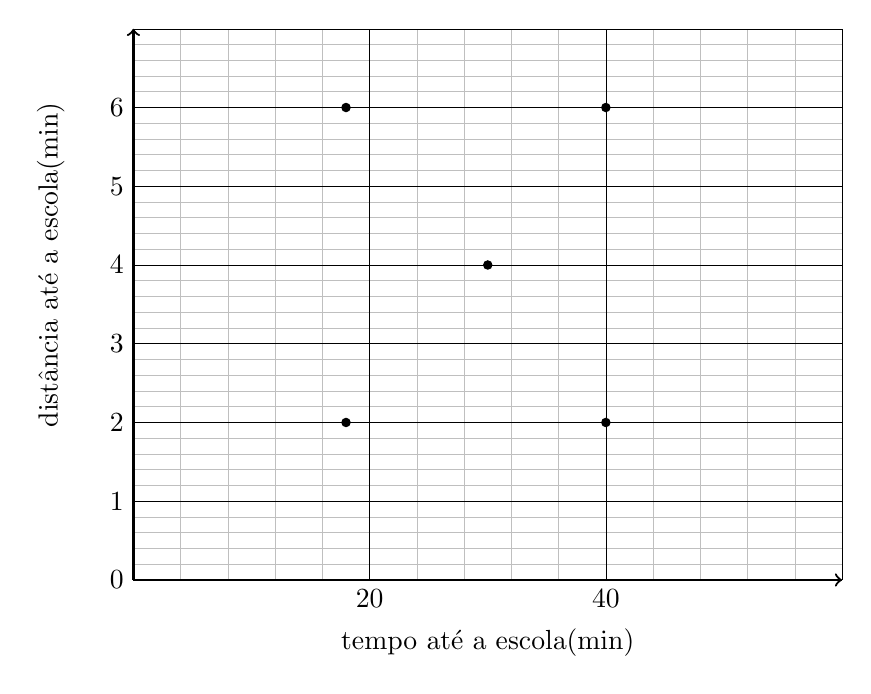
\begin{tikzpicture}
\tikzstyle{ponto}=[circle, minimum size=3pt, inner sep=0, draw=black, fill=black, shift only]
\begin{scope}[xscale=3]
\draw[help lines,xstep=.2,ystep=.2, lightgray] (0,0) grid (3,7);
\draw[help lines, black, xstep=1, ystep=1] (0,0) grid (3,7);
\draw[thick,->](0,0)--(3,0);
\draw[thick,->](0,0)--(0,7);
\draw(1.5,-.8)node{ tempo até a escola(min)};
\draw(-.35,4)node[rotate=90]{distância até a escola(min)};
\node[ponto] at(.9,2){};
\node[ponto] at(.9,6){};
\node[ponto] at(1.5,4){};
\node[ponto] at(2,2){};
\node[ponto] at(2,6){};
\foreach \y in {0,1, 2, 3, 4, 5, 6}
\draw(0,\y) [left] node {\y};
\draw(1,0)node[below]{20};
\draw(2,0)node[below]{40};
\end{scope}
\end{tikzpicture}
\end{figure}

\begin{enumerate}
\item {} 
Associe cada ponto do gráfico com o nome da criança que ele representa.

\item {} 
Como Pedro e Caetano foram para a escola na última segunda-feira? Por que?

\end{enumerate}

{\color{red}\bfseries{}{}`}\emph{{}`Adaptado de *The Language of Functions and Graphs}, Shell Centre for Mathematical Education Publications Ltd., 1985.

\end{task}

\begin{task}{ qual é o gráfico?*}
\label{\detokenize{AF106-5:ativ-qual-e-o-grafico}}\label{\detokenize{AF106-5:atividade-qual-e-o-grafico}}

Dentre os gráficos apresentados a seguir identifique aquele que melhor descreve os dados apresentados em cada uma das tabelas seguintes.


\(a)\) Café esfriando
\begin{table}[H]
\centering
\begin{tabu} to \textwidth{|c|c|c|c|c|c|c|c|}
\hline
\textbf{Tempo (minutos)} & 0 & 5 & 10 & 15 & 20 & 25 & 30 \\
\hline
\textbf{Temperatura ($^{\circ}$C)} & 90 & 79 & 70 & 62 & 55 & 49 & 44\\
\hline
\end{tabu}
\end{table}

\(b)\) Preparando a ceia

\begin{table}[H]
\centering
\begin{tabu} to \textwidth{|c|c|c|c|c|c|c|c|}
\hline
\textbf{Peso (quilos)} & 3 & 4 & 5 & 6 & 7 & 8 & 9 \\
\hline
\textbf{Tempo (horas)} & 2,5 & 3 & 3,5 & 4 & 4,5 & 5 & 5,5\\
\hline
\end{tabu}
\end{table}

\(c)\) Depois de três canecas de cerveja…

\begin{table}[H]
\centering
\begin{tabu} to \textwidth{|c|c|c|c|c|c|c|c|}
\hline
\textbf{Tempo (horas)} & 1 & 2 & 3 & 4 & 5 & 6 & 7 \\
\hline
\textbf{Álcool no sangue (mg/100ml)} & 90 & 75 & 60 & 45 & 30 & 15 & 0 \\
\hline
\end{tabu}
\end{table}

\(d)\) Como um bebê cresce antes do nascimento

\begin{table}[H]
\centering
\begin{tabu} to \textwidth{|c|c|c|c|c|c|c|c|c|}
\hline
\textbf{Tempo de gestação (meses)} & 2 & 3 & 4 & 5 & 6 & 7 & 8 & 9 \\
\hline
\textbf{Comprimento do bebê (cm)} & 4 & 9 & 16 & 24 & 30 & 34 & 38 & 42 \\
\hline
\end{tabu}
\end{table}

\begin{figure}[H]
\centering

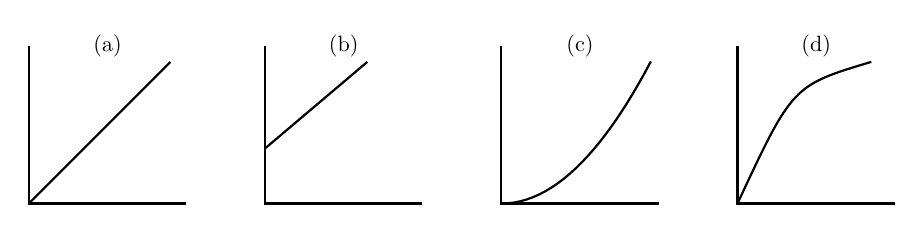
\begin{tikzpicture}
\draw[thick](0,2)--(0,0)--(2,0);
\draw(1,2)node[scale=.8]{(a)};
\draw[thick](0,0)--(1.8,1.8);
\begin{scope}[xshift=3cm]
\draw[thick](0,2)--(0,0)--(2,0);
\draw(1,2)node[scale=.8]{(b)};
\draw[thick](0,.7)--(1.3,1.8);
\begin{scope}[xshift=3cm]
\draw[thick](0,2)--(0,0)--(2,0);
\draw(1,2)node[scale=.8]{(c)};
\draw[domain=0:1.9,thick]plot(\x,.5*\x^2);
\begin{scope}[xshift=3cm]
\draw[thick](0,2)--(0,0)--(2,0);
\draw(1,2)node[scale=.8]{(d)};
\draw[thick](0,0).. controls (.7,1.5)..(1.7,1.8);
\end{scope}
\end{scope}
\end{scope}
\end{tikzpicture}

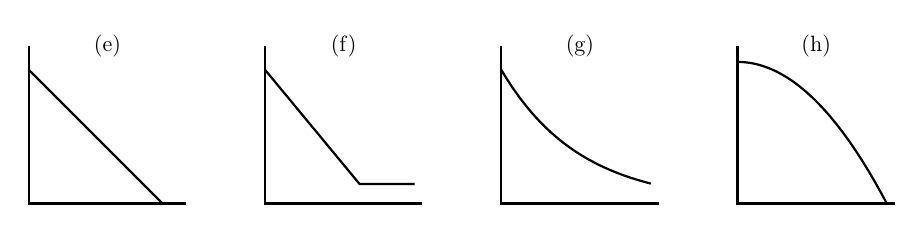
\begin{tikzpicture}
\draw[thick](0,2)--(0,0)--(2,0);
\draw(1,2)node[scale=.8]{(e)};
\draw[thick](0,1.7)--(1.7,0);
\begin{scope}[xshift=3cm]
\draw[thick](0,2)--(0,0)--(2,0);
\draw(1,2)node[scale=.8]{(f)};
\draw[thick](0,1.7)--(1.2,0.25)--(1.9,.25);
\begin{scope}[xshift=3cm]
\draw[thick](0,2)--(0,0)--(2,0);
\draw(1,2)node[scale=.8]{(g)};
\draw[domain=0:1.9,thick]plot(\x,{1.7*exp(-\x)});
\begin{scope}[xshift=3cm]
\draw[thick](0,2)--(0,0)--(2,0);
\draw(1,2)node[scale=.8]{(h)};
\draw[domain=0:1.9, thick]plot(\x,{(1.8-.5*\x^2} );
\end{scope}
\end{scope}
\end{scope}
\end{tikzpicture}

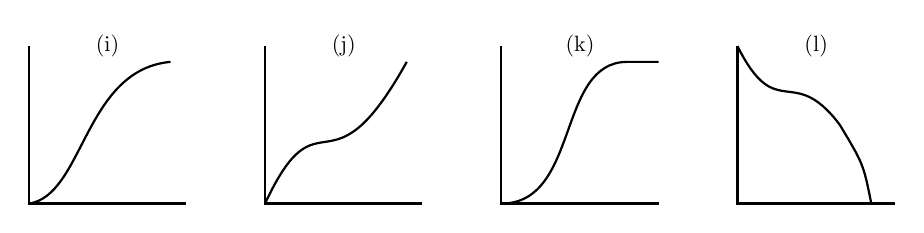
\begin{tikzpicture}
\draw[thick](0,2)--(0,0)--(2,0);
\draw(1,2)node[scale=.8]{(i)};
\draw[thick](0,0)..controls(.7,.1) and (.7,1.7) ..(1.8,1.8);
\begin{scope}[xshift=3cm]
\draw[thick](0,2)--(0,0)--(2,0);
\draw(1,2)node[scale=.8]{(j)};
\draw[thick](0,0)..controls(.7,1.5) and (.8,.0) ..(1.8,1.8);
\begin{scope}[xshift=3cm]
\draw[thick](0,2)--(0,0)--(2,0);
\draw(1,2)node[scale=.8]{(k)};
\draw[thick](0,0)..controls(1,0) and (.7,1.8) ..(1.6,1.8)..controls(1.9,1.8)..(2,1.8);
\begin{scope}[xshift=3cm]
\draw[thick](0,2)--(0,0)--(2,0);
\draw(1,2)node[scale=.8]{(l)};
\draw[thick](0,2)..controls(.5,1) and (.7,1.8) ..(1.3,1)..controls(1.6,.5)..(1.7,0);
\end{scope}
\end{scope}
\end{scope}
\end{tikzpicture}
\end{figure}

\(*\) Adaptado de \emph{The Language of Functions and Graphs}, Shell Centre for Mathematical Education Publications Ltd., 1985.
\end{task}

\begin{task}{ imaginando gráficos}
%\label{\detokenize{AF106-5:atividade-imaginando-graficos}}

Associe cada uma das situações apresentadas a seguir a um dos gráficos dados abaixo. Explique sua escolha e escreva, em cada um dos eixos, o que eles representam.
\begin{figure}[H]
\centering

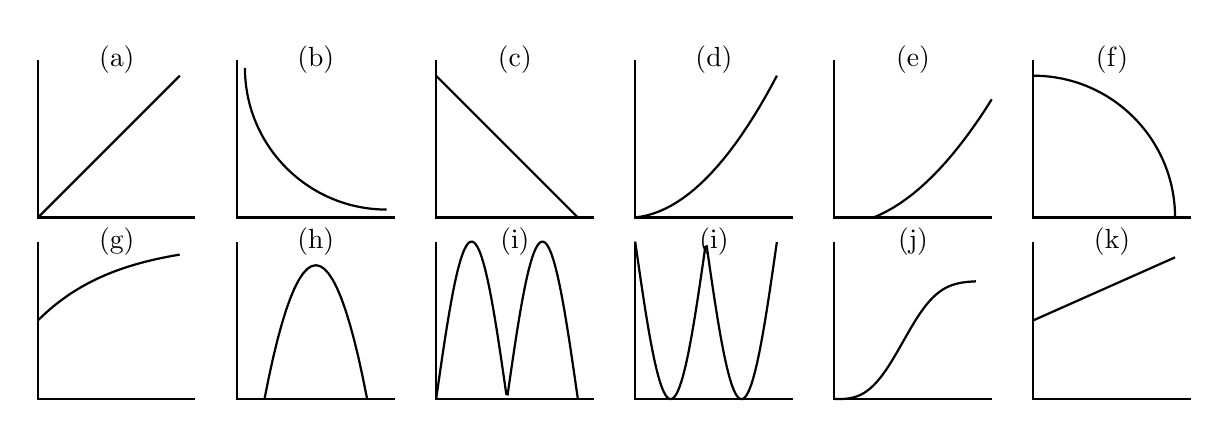
\begin{tikzpicture}
\node [matrix, column sep =.5cm] at (0,0)   {\draw[thick](0,2)--(0,0)--(2,0);\draw(1,2)node{(a)};\draw[thick](0,0)--(1.8,1.8);  &  \draw[thick](0,2)--(0,0)--(2,0);\draw(1,2)node{(b)};\draw[thick](0.1,1.9) arc(180:270:1.8);&\draw[thick](0,2)--(0,0)--(2,0);\draw(1,2)node{(c)};\draw[domain= 0:1.8,thick] plot(\x,1.8-\x); &\draw[thick](0,2)--(0,0)--(2,0);\draw(1,2)node{(d)};\draw[domain= 0:1.8,thick] plot(\x,.5*\x^2+.1*\x);&\draw[thick](0,2)--(0,0)--(2,0);\draw(1,2)node{(e)};\draw[domain= 0:2,thick] plot(\x,{max(0,.4*\x^2-.1)});&\draw[thick](0,2)--(0,0)--(2,0);\draw(1,2)node{(f)};\draw[thick](1.8,0) arc(0:90:1.8);\\  \draw[thick](0,2)--(0,0)--(2,0);\draw(1,2)node{(g)};\draw[domain=0:1.8,thick, samples=100]plot(\x, {2-exp(-\x)});& \draw[thick](0,2)--(0,0)--(2,0);\draw(1,2)node{(h)};\draw[domain=0.35:1.65,thick]plot(\x,{1.7-4*(1-\x)^2});& \draw[thick](0,2)--(0,0)--(2,0);\draw(1,2)node{(i)};\draw[domain=0:1.8, samples=100,thick]plot(\x,{abs(2*sin(200*\x))});&\draw[thick](0,2)--(0,0)--(2,0);\draw(1,2)node{(i)};\draw[domain=0:1.8, samples=100,thick]plot(\x,{2-(abs(2*sin(200*\x))});&\draw[thick](0,2)--(0,0)--(2,0);\draw(1,2)node{(j)};\draw[domain=0:1.8, samples=100,thick]plot(\x,{1.5-1.5*exp(-\x^3)});&       \draw[thick](0,2)--(0,0)--(2,0);\draw(1,2)node{(k)};\draw[thick](0,1)--(1.8,1.8);\\};
\end{tikzpicture}
\end{figure}

\begin{enumerate}[label=($\Roman*$)]
\item Após um concerto houve um grande silêncio. Então uma pessoa na platéia começou a aplaudir. Gradualmente, as pessoas à sua volta também começaram a apludir de forma que rapidamente todos estavam aplaudindo.

\item Se o preço cobrado pelo ingresso de um cinema for muito baixo, seu prorietário irá perder dinheiro. Por outro lado, se o valor cobrado for muito alto, poucas pessoas irão pagar e novamente o proprietário vai perder dinheiro. Um cinema deve portanto cobrar um preço moderado por seu ingresso de forma que seja lucrativo.

\item Preços estão agora subindo mais lentamente do que em qualquer época nos últimos cinco anos.
\end{enumerate}
\begin{itemize}
\item {} 
Adaptado do artigo \emph{Michal Ayalon \& Anne Watson \& Steve Lerman (2015). Progression Towards Functions: Students’ Performance on Three Tasks About Variables from Grades 7 to 12.}
\end{itemize}
\end{task}

\begin{reflection}{}

Observe as figuras abaixo
\begin{figure}[H]
\centering

\begin{tikzpicture}
\draw[->](0,0)--(2.5,0);
\draw[->](0,0)--(0,2.5);
\draw[domain=.2:2.2]plot (\x, \x+.2);
\foreach \x in{0.5,1,1.5}
\draw[dashed](\x,\x+.2)[->]--(\x+.5,\x+.2)--(\x+.5,\x+.7);
\foreach \x in{0.5,1,1.5}
\draw(\x+.2,\x+.15)--(\x+.2,\x+.25);
\foreach \x in{0.5,1,1.5}
\draw(\x+.25,\x+.15)--(\x+.25,\x+.25);
\begin{scope}[xshift=3cm]
\draw[->](0,0)--(2.5,0);
\draw[->](0,0)--(0,2.5);
\draw[domain=.2:2.3]plot(\x,{.3*(exp(\x))}) ;
\draw [->,dashed] (1.,0.4946163812100384) -- (1.,0.8154845485377135);
\draw [->,dashed] (1.5,0.8154845485377135) -- (1.5,1.3445067211014192);
\draw [->,dashed] (2.,1.3445067211014192) -- (2.,2.216716829679195);
\draw [dashed] (0.5,0.4946163812100384)-- (1.,0.4946163812100384);
\draw [dashed] (0.7274102214004744,0.5488318498488993) -- (0.7274102214004744,0.44040091257117747);
\draw [dashed] (0.7725897785995253,0.5488318498488993) -- (0.7725897785995253,0.44040091257117747);
\draw [dashed] (1.,0.8154845485377135)-- (1.5,0.8154845485377135);
\draw [dashed] (1.2274102214004736,0.8697000171765743) -- (1.2274102214004736,0.7612690798988525);
\draw [dashed] (1.2725897785995244,0.8697000171765743) -- (1.2725897785995244,0.7612690798988525);
\draw [dashed] (1.5,1.3445067211014192)-- (2.,1.3445067211014192);
\draw [dashed] (1.727410221400475,1.39872218974028) -- (1.727410221400475,1.290291252462558);
\draw [dashed] (1.7725897785995257,1.39872218974028) -- (1.7725897785995257,1.290291252462558);
\begin{scope}[xshift=3cm]
\draw[->](0,0)--(2.5,0);
\draw[->](0,0)--(0,2.5);
\draw[domain=.2:2.3]plot(\x,{2+(ln(\x))}) ;
\draw [->,dashed] (1.,1.3068528194400546) -- (1.,2.);
\draw [->,dashed] (1.5,2.) -- (1.5,2.4054651081081646);
\draw [->,dashed] (2.,2.4054651081081646) -- (2.,2.6931471805599454);
\draw [dashed] (0.5,1.3068528194400546)-- (1.,1.3068528194400546);
\draw [dashed] (0.7274102214004744,1.3610682880789153) -- (0.7274102214004744,1.2526373508011936);
\draw [dashed] (0.7725897785995253,1.3610682880789153) -- (0.7725897785995253,1.2526373508011936);
\draw [dashed] (1.,2.)-- (1.5,2.);
\draw [dashed] (1.2274102214004736,2.054215468638861) -- (1.2274102214004736,1.9457845313611395);
\draw [dashed] (1.2725897785995244,2.054215468638861) -- (1.2725897785995244,1.9457845313611395);
\draw [dashed] (1.5,2.4054651081081646)-- (2.,2.4054651081081646);
\draw [dashed] (1.727410221400475,2.4596805767470253) -- (1.727410221400475,2.3512496394693034);
\draw [dashed] (1.7725897785995257,2.4596805767470253) -- (1.7725897785995257,2.3512496394693034);
\end{scope}
\end{scope}
\begin{scope}[yshift=-3.5cm]
\draw[->](0,0)--(2.5,0);
\draw[->](0,0)--(0,2.5);
\draw[smooth,samples=100,domain=.2:2.2] plot(\x,{2.5-(\x)});
\draw [->,dashed] (1.,2.) -- (1.,1.5);
\draw [->,dashed] (1.5,1.5) -- (1.5,1.);
\draw [->,dashed] (2.,1.) -- (2.,0.5);
\draw [,dashed] (0.5,2.)-- (1.,2.);
\draw [dashed] (0.7274102214004744,2.054215468638861) -- (0.7274102214004744,1.9457845313611395);
\draw [dashed] (0.7725897785995253,2.054215468638861) -- (0.7725897785995253,1.9457845313611395);
\draw [dashed] (1.,1.5)-- (1.5,1.5);
\draw [dashed] (1.2274102214004736,1.5542154686388605) -- (1.2274102214004736,1.4457845313611388);
\draw [dashed] (1.2725897785995244,1.5542154686388605) -- (1.2725897785995244,1.4457845313611388);
\draw [dashed] (1.5,1.)-- (2.,1.);
\draw [dashed] (1.727410221400475,1.054215468638861) -- (1.727410221400475,0.9457845313611393);
\draw [dashed] (1.7725897785995257,1.054215468638861) -- (1.7725897785995257,0.9457845313611393);
\begin{scope}[xshift=3cm]
\draw[->](0,0)--(2.5,0);
\draw[->](0,0)--(0,2.5);
\draw[domain=.2:2.05]plot(\x,{2.5-.3*(exp(\x))}) ;
\draw [dashed] (0.7274102214004744,2.054215468638861) -- (0.7274102214004744,1.9457845313611395);
\draw [dashed] (0.7725897785995253,2.054215468638861) -- (0.7725897785995253,1.9457845313611395);
\draw [->,dashed] (1.,2.0053836187899616) -- (1.,1.6845154514622864);
\draw [->,dashed] (1.5,1.6845154514622864) -- (1.5,1.1554932788985808);
\draw [->,dashed] (2.,1.1554932788985808) -- (2.,0.2832831703208054);
\draw [dashed] (1.,1.6845154514622864)-- (1.5,1.6845154514622864);
\draw [dashed] (1.2274102214004736,1.7387309201011474) -- (1.2274102214004736,1.6302999828234255);
\draw [dashed] (1.2725897785995244,1.7387309201011474) -- (1.2725897785995244,1.6302999828234255);
\draw [dashed] (1.5,1.1554932788985808)-- (2.,1.1554932788985808);
\draw [dashed] (1.727410221400475,1.2097087475374417) -- (1.727410221400475,1.10127781025972);
\draw [dashed] (1.7725897785995257,1.2097087475374417) -- (1.7725897785995257,1.10127781025972);
\draw [dashed] (0.5,2.0053836187899616)-- (1.,2.0053836187899616);
\begin{scope}[xshift=3cm]
\draw[->](0,0)--(2.5,0);
\draw[->](0,0)--(0,2.5);
\draw[domain=.37:2.1]plot(\x,{1.0/(\x)}) ;
\draw [->,dashed] (1.,2.) -- (1.,1.);
\draw [->,dashed] (1.5,1.) -- (1.5,0.6666666666666666);
\draw [->,dashed] (2.,0.6666666666666666) -- (2.,0.5);
\draw [dashed] (0.7274102214004744,2.054215468638861) -- (0.7274102214004744,1.9457845313611395);
\draw [dashed] (0.7725897785995253,2.054215468638861) -- (0.7725897785995253,1.9457845313611395);
\draw [dashed] (1.,1.)-- (1.5,1.);
\draw [dashed] (1.2274102214004736,1.054215468638861) -- (1.2274102214004736,0.9457845313611393);
\draw [dashed] (1.2725897785995244,1.054215468638861) -- (1.2725897785995244,0.9457845313611393);
\draw [dashed] (1.5,0.6666666666666666)-- (2.,0.6666666666666666);
\draw [dashed] (1.727410221400475,0.7208821353055274) -- (1.727410221400475,0.6124511980278056);
\draw [dashed] (1.7725897785995257,0.7208821353055274) -- (1.7725897785995257,0.6124511980278056);
\draw [dashed] (0.5,2.)-- (1.,2.);
\end{scope}
\end{scope}
\end{scope}
\end{tikzpicture}
\end{figure}

O que os gráficos da primeira linha têm em comum? E as da segunda linha?

Agora observe-os por coluna. Você consegue identificar algo em comum?
\end{reflection}

\begin{description}
\item[{Função crescente e função decrescente\index{Função crescente e função decrescente|textbf}}] \leavevmode\phantomsection\label{\detokenize{AF106-5:term-funcao-crescente-e-funcao-decrescente}}
Uma função \(f: \mathbb{R} \to \mathbb{R}\) é dita \emph{crescente} quando os valores das imagens, \(f(x)\), aumentam à medida em que os valores de \(x\) aumentam, ou seja, para \(x_2>x_1\) tem-se \(f(x_2)>f(x_1)\).

\begin{figure}[H]
\centering

\begin{tikzpicture}
\draw[thick,->](-2,0)--(5,0);
\draw[thick,->](0,-1)--(0,4);
\draw[very thick,domain=-2:2.9, \currentcolor!80]plot(\x,{.5+.2*exp(\x)});
\draw[thick,dashed, ->](1,{.5+.2*exp(1)})--(2.5,{.5+.2*exp(1)})--(2.5,{.5+.2*exp(2.5)}) ;
\end{tikzpicture}
\end{figure}

E é dita \emph{decrescente} quando os valores das imagens, \(f(x)\), diminuem à medida em que os valores de \(x\) aumentam, ou seja, para \(x_2>x_1\) tem-se \(f(x_2)<f(x_1)\).
\begin{figure}[H]
\centering

\begin{tikzpicture}
\draw[thick,->](-2,0)--(5,0);
\draw[thick,->](0,-1)--(0,4);
\draw[very thick,domain=-2:3.6, \currentcolor!80]plot(\x,{3-.1*exp(\x)});
\draw[thick,dashed, ->](1,{3-.1*exp(1)})--(3,{3-.1*exp(1)})--(3,{3-.1*exp(3)}) ;
\end{tikzpicture}
\end{figure}

\end{description}


\begin{task}{ leia no gráfico!}
\label{\detokenize{AF106-5:atividade-leia-no-grafico}}\label{\detokenize{AF106-5:ativ-praticando-notacao}}

Seja \(f\) a função real cuja representação gráfica é apresentada a seguir.

\begin{figure}[H]
\centering

\begin{tikzpicture}
\tikzstyle{ponto}=[circle, minimum size=3pt, inner sep=0, draw=black, fill=black, shift only]
\draw[gray!40](0,-1.5)grid[xstep=.25,ystep=.25,line width =1pt](5.5,3);
\draw(0,-1.5)grid[xstep=1,ystep=1,line width =1pt, help lines](5.5,3);
\draw[->,thick](-.5,0)--(5.5,0) node[right]{$x$};
\draw[->,thick](0,-1.5)--(0,3)node[above]{$y$};
\draw[very thick, \currentcolor!80](0,-.5)--(.5,1)--(1,1.5)--(1.5,1.5)--(2,.5)--(2.5,0)--(3,-1)--(4,2)--(4.5,2.5)--(5,2.75);
\foreach \x in{2, 4, 6, ..., 10}
\draw(.5*\x,0)[below]node{\x};
\foreach \y in{-2, 2,4,6}
\draw(0,.5*\y)[left]node{\y};
\node[below left]at (0,0){0};
\end{tikzpicture}
\end{figure}

A partir da representação gráfica calcule os seguintes valores:

\begin{table}[H]
\centering
\begin{tabu} to \textwidth{|l|c|}
\hline
\thead
Notação & Valor \\
\hline
\(f(1)-f(0)\) & \\
\hline
\(4\cdot f(3)\) & \\
\hline
\(f(4)/f(2)\) & \\
\hline
\(f(6)\cdot f(2)\) & \\
\hline
\(x\) quando \(f(x)=-2\) & \\
\hline
\(x\) quando \(f(x)=0\) & \\
\hline
\(f(3\cdot 2)-4\cdot f(\sqrt{81})+1\) & \\
\hline
\end{tabu}
\end{table}

\end{task}

\begin{reflection}{}

Observe o gráfico da função real dada pela expressão \(f(x)=3x^2-15x+18\). Veja que ele possui interseções com o eixo das abscissas e com o eixo das ordenadas. Qual procedimento você utilizaria para determinar esses pontos de interseção?
\begin{center}\begin{tikzpicture}
\draw[->, thick](-.5,0)--(4,0);
\draw[->,thick](0,-.5)--(0,6);
\draw[very thick, domain=-.2:3.7, samples=100, \currentcolor!80]plot(\x,{1.5*(\x-1.5)*(\x-2)});
\end{tikzpicture}\end{center}
Os valores de \(x\) para os quais há interseção com o eixo das abscissas são chamados de \emph{zeros} da função.
\end{reflection}

\begin{task}{Imposto de renda}

A seguinte tabela é utilizada para o cálculo do Imposto de Renda para Pessoa Física (IRPF).

\begin{table}[H]
\centering

\large{\textbf{Tabela do IRF - Vigência a partir de 01/04/2015}}

(Medida Provisória 670/2015 convertida na Lei 13.149/2015)
\begin{tabu} to \textwidth{|l|c|r|}
\hline
\thead
Base de cálculo (R\$) & Alíquota (\%) & Parcela a deduzir do IR (R\$) \\
\hline
Até $1.903{,}98$ & - & - \\
\hline
De $1.903{,}99$ até $2.826{,}65$ & 7,5 & $142{,}80$ \\
\hline
De 2$.825{,}55$ até $3.751{,}05$ & 15 & $354{,}80$ \\
\hline
$3.751{,}06$ até $4.664{,}68$ & 22,5 & $636{,}13$ \\
\hline
Acima de $4.664{,}68$ & 27,5 & $869{,}36$ \\
\hline
\end{tabu}
\caption{Fonte: \url{http://www.portaltributario.com.br}}
\end{table}

Por esta tabela, um trabalhador cujo rendimento é inferior a R\$ $1.903{,}98$ está isento do imposto de renda. Já um trabalhador com rendimento de R\$$3.000{,}00$ tem um desconto, em reais, de $15\%$ de $3.000{,}00$ (450,00) menos a dedução de 354,80, isto é, deverá pagar de importo de renda o valor $450-354{,}80=95{,}20$R\$.

\begin{enumerate}
\item Com os dados apresentados na tabela acima construímos a seguinte função que fornece o valor de importo de renda a ser pago, a partir do rendimento informado:
\[f(x)=
\begin{cases}
0, \text{ se } x\leq1.903{,}98\\
0{,}075x-142{,}90, \text{ se } 1.903{,}98<x<2.826{,}65\\
0{,}15x-354{,}90, \text{ se } 2.826{,}65\leq x<3.751{,}05\\
0{,}225x-636{,}13 \text{ se } 3.751{,}05 \leq x<4.664{,}68\\
0{,}275x-869{,}36 \text{ se } 4.664{,}68\leq x
\end{cases}
\]

Determine o imposto que deverá ser pago por um trabalhador cujo rendimento seja:
\begin{enumerate}
\item R\$$1.750{,}00$
\item R\$$2.680{,}00$
\item R\$$4.060{,}00$
\item R\$$5.500{,}00$
\end{enumerate}

\item Observe o gráfico a seguir. Nele estão destacados os impostos de renda pago por três trabalhadores, indicados pelas letras $A$, $B$ e $C$.

\begin{figure}[H]
\centering

\begin{tikzpicture}[xscale=.2,yscale=1.25]
\draw [->] (0,0) -- (52,0) node [below left, scale=.75] {Salários (R\$)};
\draw [->] (0,0) -- (0,5) node [above left, rotate=90, scale=.75] {Imposto (R\$)};

\draw [thick, \currentcolor!80] (0,0) -- (19.0390,0) -- (28.2665,28.25665*.075-1.428) -- (37.506,37.056*.15-3.548) -- (46.64468,46.64468*.225-6.3613) -- (50,50*.275-8.6936);

\draw [dashed,\currentcolor!80](28.2665,28.25665*.075-1.428) -- (28.2665,0);
\draw [dashed,\currentcolor!80] (37.506,37.056*.15-3.548) -- (37.506,0);
\draw [dashed,\currentcolor!80](46.64468,46.6468*.225-6.3613) -- (46.64468,0);

\draw [dashed] (0,.552) -- (26,.552) -- (26,0);
\draw [dashed] (0,1.522) -- (34,1.552) -- (34,0);
\draw [dashed] (0,2.6387) -- (40.3,2.6387) -- (40.3,0); 

\node (a) [circle,fill, inner sep=1pt,label=above:A] at (26,.522) {};
\node (b) [circle,fill, inner sep=1pt, label=above:B] at (34,1.522) {};
\node (c) [circle,fill, inner sep=1pt, label=above:C, xshift=.5mm] at (40,2.6387) {};

\node [left] at (0,.522) {52,20};
\node [left] at (0,1.5520) {155,20};
\node [left] at (0,2.6387) {263,87};
\end{tikzpicture}
\end{figure}

Segundo a tabela IRF, determine as alíquotas de desconto que estão sendo aplicadas a cada um destes trabalhadores e qual o salário de cada um deles.
\end{enumerate}

\end{task}

\begin{task}{Planos telefônicos}

Você deseja trocar o plano do seu telefone e ao consultar a sua operadora tem a opção de escolher entre dois planos: plano Prata e plano Ouro. No seu plano atual, você paga R\$$70{,}00$ por 500MB de internet e os dados além disso custam R\$$0{,}20$ por MB. 

O plano Ouro cobra R\$$140{,}00$ por dados ilimitados e o plano Prata tem a mesma estrutura do seu plano atual. Os valores cobrados pelo plano Prata estão representados no gráfico a seguir.

\begin{figure}[H]
\centering


\begin{tikzpicture}[yscale=.5,scale=.75, every node/.style={scale=.75}]

\draw [->] (0,0) -- (14,0) node [below left, yshift=-.5cm] {Dados (MB)};
\draw [->] (0,0) -- (0,20) node [above left, rotate=90, yshift=.5cm] {Valor (R\$)};
\draw [help lines] (0,0) grid (14,20);

\foreach \x in {2,4,...,20} \node [left] at (0,\x) {\x0};
\foreach \x in {1,2,...,14} \node [below] at (\x,0) {\x00};

\node [below left] at (0,0) {0};

\draw [thick, \currentcolor!80] (0,8) -- (6,8) -- (14,20);

\end{tikzpicture}
\end{figure}

\begin{enumerate}
\item Qual o valor fixo cobrado no plano Prata e que quantidade de dados ele cobre?
\item Qual o valor por MB excedente do valor estipulado?
\item A partir de que quantidade de dados consumidos o plano Ouro passa a ser mais vantajoso?
\item Represente no sistema de coordenadas acima o gráfico do preço a pagar pelo plano Ouro.
\end{enumerate}

\end{task}

\begin{task}{Bandeiras tarifárias}

Desde o ano de 2015, as contas de energia passaram a trazer uma novidade: o Sistema de Bandeiras Tarifárias, que apresenta as seguintes modalidades: verde, amarela e vermelha - as mesmas cores dos semáforos - e indicam se haverá ou não acréscimo no valor de energia a ser repassada ao consumidor final, em função das condições de geração de eletricidade. Cada modalidade apresenta as seguintes características:

%adicionar bandeiras
\begin{itemize}
\item \textbf{Bandeira verde}: condições favoráveis de geração de energia. A tarifa não sofre nenhum acréscimo;

\item \textbf{Bandeira amarela}: condições de geração menos favoráveis. A tarifa sobre acréscimo de R\$$0{,}01343$ para cada quilowatt-hora (kWh) consumidos;

\item \textbf{Bandeira vermelha - patamar 1}: condições mais custosas de geração. A tarifa sofre acréscimo de R\$$0{,}04169$ para cada quilowatt-hora (kWh) consumido.

\item \textbf{Bandeira vermelha - patamar 2}: condições mais custosas de geração. A tarifa sofre acréscimo de R\$$0{,}06243$ para cada quilowatt-hora (kWh) consumido.
\end{itemize}

\flushright{\small

Texto extraído da página da ANEEL em 28/03/2020 \\ \url{https://www.aneel.gov.br/bandeiras-tarifárias}}

\justify
O sistema de coordenadas abaixo contém os gráficos para as funções que relacionam o preço a pagar pela energia em relação ao consumo em quilowatt-hora (kWh) para cada uma das bandeiras tarifárias, em uma cidade vizinha. Com base nas informações do gráfico a seguir, responda:

\begin{figure}[H]
\centering

\begin{tikzpicture}[yscale=2.5,scale=.75, every node/.style={scale=.75}]

\draw [->] (0,5) -- (11,5) node [below left, yshift=-.5cm] {consumo (kWh)};
\draw [->] (0,5) -- (0,9) node [above left, , rotate=90, yshift=1.2cm] {Preço a pagar (R\$)};

\foreach \x in {2,4,...,10} {\node [below] at (\x,5) {\x00};
\draw [help lines] (\x,5) -- (\x,9);
};
\foreach \x/\y in {8/{800,00},8.1343/{813,43},8.4169/{841,89},8.6243/{862,43}} {

\node [left] at (0,\x) {\y};

\draw [thick, \currentcolor!80] (0,5) -- (10,\x);
\draw [help lines] (0,\x) -- (10,\x);
};

\end{tikzpicture}
\end{figure}

\end{task}

\know{}
\label{\detokenize{AF106-A::doc}}\label{\detokenize{AF106-A:para-saber-mais}}\label{\detokenize{AF106-A:sec-aprofundando-grafico}}

\begin{task}{ Todo mundo tem \emph{Facebook}?}
\label{\detokenize{AF106-A:atividade-todo-mundo-tem-facebook}}\label{\detokenize{AF106-A:ativ-todo-mundo-tem-facebook}}

A rede social virtual \emph{Facebook} é um grande sucesso. O Facebook criado por Mark Zuckerberg em outubro de 2003, com o nome de \emph{Facemash}, quando ele era  um estudante do segundo ano em Harvard. Inicialmente \(450\) visitantes geraram \(22.000\) visualizações de fotos em suas primeiras \(4\) horas online. Em fevereiro de \(2004\), agora com o nome de \emph{Thefacebook}, ele já contava com a participação de mais da metade dos alunos de Harvard, e um mês depois, estudantes das Universidades de Stanford, Columbia, Yale, Boston, Nova Iorque e MIT tiveram acesso à rede social criada por Mark Zuckerberg. A partir de setembro de \(2005\), funcionários de várias empresas, dentre elas \emph{Apple} e \emph{Microsoft}, puderam ter acesso ao \emph{Facebook} e no final de \(2006\) o serviço ficou disponível para qualquer pessoa maior de \(13\) anos e com um endereço válido de \emph{e-mail}.

A tabela a seguir mostra o número de usuários ativos do \emph{Facebook} em janeiro dos anos de \(2004\) a \(2015\).

\begin{table}[H]
\centering
\begin{tabu} to \textwidth{|c|l|c|}
\hline
\thead
Ano & Número de usuários & Crescimento percentual \\
\hline
2004 & 5 & \textendash{} \\
\hline
2005 & 1.000.000 & \\
\hline
2006 & 5.500.000 & 450\% \\
\hline
2007 & 12.000.000 & \\
\hline
2008 & 70.000.000 & \\
\hline
2009 & 150.000.000 & \\
\hline
2010 & 370.000.000 & \\
\hline
2011 & 600.000.000 & \\
\hline
2012 & 800.000.000 & \\
\hline
2013 & 1.056.000.000 & \\
\hline
2014 & 1.228.000.000 & \\
\hline
2015 & 1.317.000.000 & \\
\hline
\end{tabu}
\end{table}


Imagine que queremos investigar o crescimento anual do número de usuários. E, a partir da investigação formular um modelo que nos permita fazer previsões sobre a base de usuários para os próximos anos.
\begin{enumerate}
\item {} 
Vamos começar investigando o crescimento percentual, preenchendo as lacunas da terceira coluna da tabela acima.

\item {} 
Marque no plano cartesiano os pontos correspondentes aos dados fornecidos pelas duas primeiras colunas da tabela, usando a seguinte escala: no eixo das abscissas \(1\) cm corresponde a \(1\) ano e no eixo das ordenadas \(1\) cm corresponde a \(200\) milhões de usuários ativos.

\item {} 
Como você descreveria o crescimento do número de usuários ativos do \emph{Facebook}? Você acha que o crescimento está com tendência a diminuir, a aumentar ou a permanecer estável?

\item {} 
Baseado no item c), faça uma previsão para o número de usuários para os anos de 2016 e 2017.

\item {} 
Usando os dados da tabela e a representação gráfica feita no item b), faça uma previsão para o futuro do \emph{Facebook}. Você acha que os números continuarão a aumentar? Se sim, quando ele atingirá a marca de \(2\) bilhões de usuários? Explique seu raciocínio.

\item {} 
Um modelo matemático que fornece uma aproximação para a relação entre os dados das duas primeiras colunas da tabela é dado por uma função \(f\) que tem a seguinte expressão
\begin{equation*}
\begin{split}f(x)=\dfrac{980}{0,7+670 \cdot 0,45^{(x+1)}}\end{split}
\end{equation*}
em que \(x\) representa o tempo decorrido desde \(2004\), isto é, para \(2010\) tem-se \(x=6\), e \(f(6)\) é o valor em milhões de usuários ativos no \emph{Facebook} naquele ano. Com a ajuda de uma calculadora científica, use a expressão acima para calcular a estimativa do número de usuários nos anos de \(2013\) e de \(2014\), e em seguida compare com a tabela.

\item {} 
Use a expressão anterior e calcule a estimativa para os anos de \(2016\) e \(2017\) e compare com as suas previsões do item (d).

\end{enumerate}

Os dados reais para os meses de janeiro de \(2016\) e \(2017\) são \(1.654.000.000\) e \(1.936.000.000\), respectivamente. Isso significa que apesar do modelo descrever de forma satisfatória o comportamento do crescimento do número de usuários até o ano de \(2015\), para os anos seguintes ele não se mostra adequado. Existia de fato uma tendência para diminuição do crescimento, no entanto essa trajetória foi possivelmente modificada por ações que foram tomadas pela empresa ao perceber tal comportamento.

Situações como essa são bastante comuns em Modelagem Matemática. O modelo se mostra adequado sob certas condições, mas quando outras variáveis são consideradas (investimento em propaganda, alteração no algoritmo que escolhe as atualizações que serão exibidas para cada usuário, etc) ele pode perder sua acurácia, momento em que se fazem necessárias revisões.

\end{task}

\begin{task}{ Decodificando a mensagem}
\label{\detokenize{AF106-A:atividade-decodificando-a-mensagem}}\label{\detokenize{AF106-A:ativ-decodificando}}

Um dos conceitos mais importantes para a segurança na \emph{internet} nos dias de de hoje é o que chamamos de \textbf{criptografia} (do grego \emph{criptos} = escondido, \emph{grafia} = escrita). Segundo o site \emph{wikipedia} ela é o estudo dos princípios e técnicas pelas quais a informação pode ser transformada da sua forma original para outra codificada, de forma que possa ser conhecida apenas por seu destinatário (detentor da “chave secreta”), o que a torna difícil de ser decifrada por alguém não autorizado. Em outras palavras, cria-se um código que pode ser facilmente desfeito (decodificado) mas apenas por aqueles que conhecem a codificação.

Considere a seguinte maneira de codificar o alfabeto

\begin{table}[H]
\centering
\setlength\tabcolsep{3pt}
\begin{tabu} to \textwidth{|c|c|c|c|c|c|c|c|c|c|c|c|c|c|c|c|c|c|c|c|c|c|c|c|c|c|c|}
\hline
\cellcolor{\currentcolor!80}{\textcolor{black}{\textbf{Original}}} & A & B & C & D & E & F & G & H & I & J & K & L & M & N & O & P & Q & R & S & T & U & V & W & X & Y & Z \\
\hline
\cellcolor{\currentcolor!80}{\textcolor{black}{\textbf{Código}}} & P & Q & R & S & T & U & V & W & X & Y & Z & A & B & C & D & E & F & G & H & I & J & K & L & M & N & O \\
\hline
\end{tabu}
\end{table}

\begin{enumerate}
\item {} 
Use o código acima para codificar a palavra IMAGEM.

\item {} 
Se você recebesse uma mensagem com a expressão RGXEIDVGPUPG, como faria para decodificá-la?

A codificação acima pode também ser representada em um gráfico em que no eixo horizontal estão as letras originais e no vertical os seus respectivos códigos.

\begin{figure}[H]
\centering

\begin{tikzpicture}
\draw[scale=.5](0,0)grid(26,26);
\foreach \i [count=\x from 0] in{{A}, {B},{C}, {D}, {E}, {F}, {G}, {H},{I},{J},{K},{L},{M},{N},{O},{P},{Q},{R},{S},{T},{U},{V},{W},{X},{Y},{Z}}
\draw (.2+.5*\x,-.4) node {\i};
\foreach \i [count=\x from 0] in{{A}, {B},{C}, {D}, {E}, {F}, {G}, {H},{I},{J},{K},{L},{M},{N},{O},{P},{Q},{R},{S},{T},{U},{V},{W},{X},{Y},{Z}}
\draw (-.4,.2+.5*\x) node {\i};
\fill[color=\currentcolor!80](5.5,0)--(6,0)--(6,.5)--(5.5,.5);
\fill[color=\currentcolor!80](6,.5)--(6.5,.5)--(6.5,1)--(6,1);
\fill[color=\currentcolor!80](6.5,1)--(7,1)--(7,1.5)--(6.5,1.5);
\fill[color=\currentcolor!80](7,1.5)--(7.5,1.5)--(7.5,2)--(7,2);
\fill[color=\currentcolor!80] ( 7.5 , 2.0 )--( 8.0 , 2.0 )--( 8.0 , 2.5 )--( 7.5 , 2.5 );
\fill[color=\currentcolor!80] ( 8.0 , 2.5 )--( 8.5 , 2.5 )--( 8.5 , 3.0 )--( 8.0 , 3.0 );
\fill [color=\currentcolor!80]( 8.5 , 3.0 )--( 9.0 , 3.0 )--( 9.0 , 3.5 )--( 8.5 , 3.5 );
\fill [color=\currentcolor!80]( 9.0 , 3.5 )--( 9.5 , 3.5 )--( 9.5 , 4.0 )--( 9.0 , 4.0 );
\fill [color=\currentcolor!80]( 9.5 , 4.0 )--( 10.0 , 4.0 )--( 10.0 , 4.5 )--( 9.5 , 4.5 );
\fill [color=\currentcolor!80]( 10.0 , 4.5 )--( 10.5 , 4.5 )--( 10.5 , 5.0 )--( 10.0 , 5.0 );
\fill[color=\currentcolor!80] ( 10.5 , 5.0 )--( 11.0 , 5.0 )--( 11.0 , 5.5 )--( 10.5 , 5.5 );
\fill[color=\currentcolor!80] ( 11.0 , 5.5 )--( 11.5 , 5.5 )--( 11.5 , 6.0 )--( 11.0 , 6.0 );
\fill[color=\currentcolor!80] ( 11.5 , 6.0 )--( 12.0 , 6.0 )--( 12.0 , 6.5 )--( 11.5 , 6.5 );
\fill[color=\currentcolor!80] ( 12.0 , 6.5 )--( 12.5 , 6.5 )--( 12.5 , 7.0 )--( 12.0 , 7.0 );
\fill[color=\currentcolor!80] ( 12.5 , 7.0 )--( 13.0 , 7.0 )--( 13.0 , 7.5 )--( 12.5 , 7.5 );
\fill[color=\currentcolor!80] ( 0.0 , 7.5 )--( 0.5 , 7.5 )--( 0.5 , 8.0 )--( 0.0 , 8.0 );
\fill[color=\currentcolor!80] ( 0.5 , 8.0 )--( 1.0 , 8.0 )--( 1.0 , 8.5 )--( 0.5 , 8.5 );
\fill[color=\currentcolor!80] ( 1.0 , 8.5 )--( 1.5 , 8.5 )--( 1.5 , 9.0 )--( 1.0 , 9.0 );
\fill[color=\currentcolor!80] ( 1.5 , 9.0 )--( 2.0 , 9.0 )--( 2.0 , 9.5 )--( 1.5 , 9.5 );
\fill[color=\currentcolor!80] ( 2.0 , 9.5 )--( 2.5 , 9.5 )--( 2.5 , 10.0 )--( 2.0 , 10.0 );
\fill[color=\currentcolor!80] ( 2.5 , 10.0 )--( 3.0 , 10.0 )--( 3.0 , 10.5 )--( 2.5 , 10.5 );
\fill[color=\currentcolor!80] ( 3.0 , 10.5 )--( 3.5 , 10.5 )--( 3.5 , 11.0 )--( 3.0 , 11.0 );
\fill[color=\currentcolor!80] ( 3.5 , 11.0 )--( 4.0 , 11.0 )--( 4.0 , 11.5 )--( 3.5 , 11.5 );
\fill[color=\currentcolor!80] ( 4.0 , 11.5 )--( 4.5 , 11.5 )--( 4.5 , 12.0 )--( 4.0 , 12.0 );
\fill[color=\currentcolor!80] ( 4.5 , 12.0 )--( 5.0 , 12.0 )--( 5.0 , 12.5 )--( 4.5 , 12.5 );
\fill[color=\currentcolor!80] ( 5.0 , 12.5 )--( 5.5 , 12.5 )--( 5.5 , 13.0 )--( 5.0 , 13.0 );
\draw(12.3,-1)node{alfabeto};
\draw(-1,12.3) node[rotate=90.]{C\'{o}digo};
\end{tikzpicture}
\end{figure}
\item {} 
Usando ainda o código acima escreva uma mensagem codificada com duas ou três palavras e troque com algum colega seu de classe. Decodifique a mensagem que recebeu.

Você deve ter percebido que a codificação é uma função do conjunto das letras do alfabeto em si mesmo: todas as letras precisam ter um código e uma mesma letra não pode ter mais de um código associada a si.

\item {} 
Seja \(X\) o conjunto dos números naturais de \(1\) a \(26\). Fazendo a correspondência, \(A \mapsto 1, B \mapsto 2, C \mapsto 3\), e assim por diante até \(Z \mapsto 26\), determine uma função \(f:X\to X\) que corresponda ao código acima. Observe que por exemplo, \(f(1)=16\).

\item {} 
Usando a expressão \(f(x)=x^2\) crie um novo código entre as letras, representando-o no gráfico. O que devemos fazer quando os valores são  maiores que 26?

\item {} 
Considerando o código do gráfico abaixo, tente decodificar a palavra APQGJXV.

\begin{figure}[H]
\centering

\begin{tikzpicture}
\draw[scale=.5](0,0)grid(26,26);
\foreach \i [count=\x from 0] in{{A}, {B},{C}, {D}, {E}, {F}, {G}, {H},{I},{J},{K},{L},{M},{N},{O},{P},{Q},{R},{S},{T},{U},{V},{W},{X},{Y},{Z}}
\draw (.2+.5*\x,-.4) node {\i};
\foreach \i [count=\x from 0] in{{A}, {B},{C}, {D}, {E}, {F}, {G}, {H},{I},{J},{K},{L},{M},{N},{O},{P},{Q},{R},{S},{T},{U},{V},{W},{X},{Y},{Z}}
\draw (-.4,.2+.5*\x) node {\i};
\fill[color=\currentcolor!80] ( 0.0 , 1.5 )--( 0.5 , 1.5 )--( 0.5 , 2.0 )--( 0.0 , 2.0 );
\fill[color=\currentcolor!80] ( 0.5 , 2.0 )--( 1.0 , 2.0 )--( 1.0 , 2.5 )--( 0.5 , 2.5 );
\fill[color=\currentcolor!80] ( 1.0 , 2.5 )--( 1.5 , 2.5 )--( 1.5 , 3.0 )--( 1.0 , 3.0 );
\fill[color=\currentcolor!80] ( 1.5 , 3.0 )--( 2.0 , 3.0 )--( 2.0 , 3.5 )--( 1.5 , 3.5 );
\fill[color=\currentcolor!80] ( 2.0 , 3.5 )--( 2.5 , 3.5 )--( 2.5 , 4.0 )--( 2.0 , 4.0 );
\fill[color=\currentcolor!80] ( 2.5 , 4.0 )--( 3.0 , 4.0 )--( 3.0 , 4.5 )--( 2.5 , 4.5 );
\fill[color=\currentcolor!80] ( 3.0 , 4.5 )--( 3.5 , 4.5 )--( 3.5 , 5.0 )--( 3.0 , 5.0 );
\fill[color=\currentcolor!80] ( 3.5 , 5.0 )--( 4.0 , 5.0 )--( 4.0 , 5.5 )--( 3.5 , 5.5 );
\fill[color=\currentcolor!80] ( 4.0 , 0.0 )--( 4.5 , 0.0 )--( 4.5 , 0.5 )--( 4.0 , 0.5 );
\fill[color=\currentcolor!80] ( 4.5 , 0.5 )--( 5.0 , 0.5 )--( 5.0 , 1.0 )--( 4.5 , 1.0 );
\fill[color=\currentcolor!80] ( 5.0 , 1.0 )--( 5.5 , 1.0 )--( 5.5 , 1.5 )--( 5.0 , 1.5 );
\fill[color=\currentcolor!80] ( 5.5 , 1.5 )--( 6.0 , 1.5 )--( 6.0 , 2.0 )--( 5.5 , 2.0 );
\fill[color=\currentcolor!80] ( 6.0 , 2.0 )--( 6.5 , 2.0 )--( 6.5 , 2.5 )--( 6.0 , 2.5 );
\fill[color=\currentcolor!80] ( 6.5 , 2.5 )--( 7.0 , 2.5 )--( 7.0 , 3.0 )--( 6.5 , 3.0 );
\fill[color=\currentcolor!80] ( 7.0 , 3.0 )--( 7.5 , 3.0 )--( 7.5 , 3.5 )--( 7.0 , 3.5 );
\fill[color=\currentcolor!80] ( 7.5 , 3.5 )--( 8.0 , 3.5 )--( 8.0 , 4.0 )--( 7.5 , 4.0 );
\fill[color=\currentcolor!80] ( 8.0 , 4.0 )--( 8.5 , 4.0 )--( 8.5 , 4.5 )--( 8.0 , 4.5 );
\fill[color=\currentcolor!80] ( 8.5 , 4.5 )--( 9.0 , 4.5 )--( 9.0 , 5.0 )--( 8.5 , 5.0 );
\fill[color=\currentcolor!80] ( 9.0 , 5.0 )--( 9.5 , 5.0 )--( 9.5 , 5.5 )--( 9.0 , 5.5 );
\fill[color=\currentcolor!80] ( 9.5 , 5.5 )--( 10.0 , 5.5 )--( 10.0 , 6.0 )--( 9.5 , 6.0 );
\fill[color=\currentcolor!80] ( 10.0 , 6.0 )--( 10.5 , 6.0 )--( 10.5 , 6.5 )--( 10.0 , 6.5 );
\fill[color=\currentcolor!80] ( 10.5 , 6.5 )--( 11.0 , 6.5 )--( 11.0 , 7.0 )--( 10.5 , 7.0 );
\fill[color=\currentcolor!80] ( 11.0 , 7.0 )--( 11.5 , 7.0 )--( 11.5 , 7.5 )--( 11.0 , 7.5 );
\fill[color=\currentcolor!80] ( 11.5 , 10.0 )--( 12.0 , 10.0 )--( 12.0 , 10.5 )--( 11.5 , 10.5 );
\fill[color=\currentcolor!80] ( 12.0 , 10.5 )--( 12.5 , 10.5 )--( 12.5 , 11.0 )--( 12.0 , 11.0 );
\fill[color=\currentcolor!80] ( 12.5 , 11.0 )--( 13.0 , 11.0 )--( 13.0 , 11.5 )--( 12.5 , 11.5 );
\draw(12.3,-1)node{alfabeto};
\draw(-1,12.3) node[rotate=90.]{C\'{o}digo};
\end{tikzpicture}
\end{figure}

\item {} 
Quais letras do código acima são impossíveis de decodificar e por quê?

\item {} 
Que propriedades deve ter um código para que seja possível decodificá-lo?

\end{enumerate}

\end{task}

\section{Projeto Aplicado}
\label{\detokenize{AF106-A:projeto-aplicado}}\label{\detokenize{AF106-A:sec-projeto-aplicado}}

\textbf{Como construir uma caixa de volume máximo?}

Vamos utilizar uma folha de cartolina quadrada de lado \(40\) cm para construir uma caixa sem tampa. Para isso, cortamos quadrados nos quatro cantos da cartolina e dobramos as partes retangulares restantes, para formar os lados da caixa. O objetivo é obter a caixa com o maior volume possível.

\begin{figure}[H]
\centering

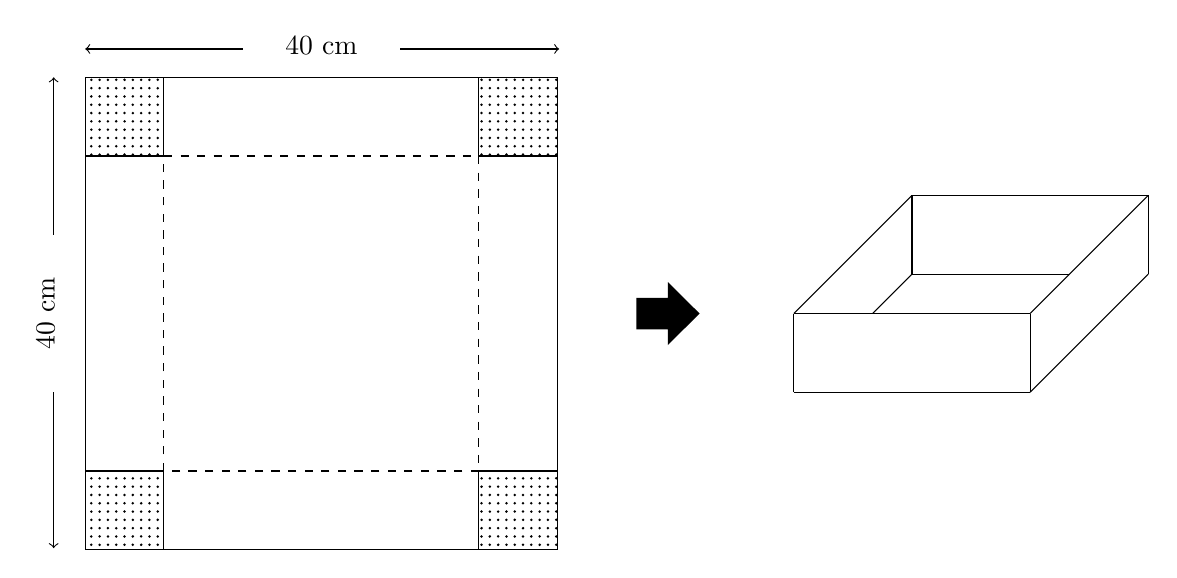
\begin{tikzpicture}
\usetikzlibrary[patterns]
\fill[fill=black,pattern=dots,pattern color=black] (-3.,3.) -- (-2.,3.) -- (-2.,2.) -- (-3.,2.) -- cycle;
\fill[fill=black,pattern=dots,pattern color=black] (-3.,-2.) -- (-2.,-2.) -- (-2.,-3.) -- (-3.,-3.) -- cycle;
\fill[fill=black,pattern=dots,pattern color=black] (2.,-3.) -- (2.,-2.) -- (3.,-2.) -- (3.,-3.) -- cycle;
\fill[line width=2.pt,fill=black,pattern=dots,pattern color=black] (2.,2.) -- (2.,3.) -- (3.,3.) -- (3.,2.) -- cycle;
\draw [line width=0.4pt, dashed] (-2.,2.)-- (2.,2.);
\draw [line width=0.4pt,dashed] (2.,2.)-- (2.,-2.);
\draw [line width=0.4pt,dashed] (2.,-2.)-- (-2.,-2.);
\draw [line width=0.4pt,dashed] (-2.,-2.)-- (-2.,2.);
\draw [line width=0.4pt] (-3.,2.)-- (-3.,-2.);
\draw [line width=0.4pt] (-2.,-3.)-- (2.,-3.);
\draw [line width=0.4pt] (3.,-2.)-- (3.,2.);
\draw [line width=0.4pt] (2.,3.)-- (-2.,3.);
\draw [line width=0.4pt] (-3.,3.)-- (-2.,3.);
\draw [line width=0.4pt] (-2.,3.)-- (-2.,2.);
\draw [line width=0.4pt] (-2.,2.)-- (-3.,2.);
\draw [line width=0.4pt] (-3.,2.)-- (-3.,3.);
\draw [line width=0.4pt] (-3.,-2.)-- (-2.,-2.);
\draw [line width=0.4pt] (-2.,-2.)-- (-2.,-3.);
\draw [line width=0.4pt] (-2.,-3.)-- (-3.,-3.);
\draw [line width=0.4pt] (-3.,-3.)-- (-3.,-2.);
\draw [line width=0.4pt] (2.,-3.)-- (2.,-2.);
\draw [line width=0.4pt] (2.,-2.)-- (3.,-2.);
\draw [line width=0.4pt] (3.,-2.)-- (3.,-3.);
\draw [line width=0.4pt] (3.,-3.)-- (2.,-3.);
\draw [line width=0.4pt] (2.,2.)-- (2.,3.);
\draw [line width=0.4pt] (2.,3.)-- (3.,3.);
\draw [line width=0.4pt] (3.,3.)-- (3.,2.);
\draw [line width=0.4pt] (3.,2.)-- (2.,2.);
\draw [<-,line width=0.4pt] (-3.4,-2.98) -- (-3.4,-1.);
\draw [->,line width=0.4pt] (-3.4,1) -- (-3.4,3.);
\draw (-3.5,0) node[rotate=90] {40 cm};
\draw [<-,line width=0.4pt] (-3.,3.36) -- (-1,3.36);
\draw [->,line width=0.4pt] (1,3.36) -- (3.02,3.36);
\draw (0,3.4) node {40 cm};
\begin{scope}[xshift=4cm]
\fill[line width=2.pt,fill=black,fill opacity=1.0] (0.,-0.2) -- (0.,0.2) -- (0.4,0.2) -- (0.4,0.4) -- (0.8025630171471898,0.) -- (0.4,-0.4) -- (0.4,-0.2) -- cycle;
\begin{scope}[xshift=2cm, yshift=-1cm]
\draw [line width=.4pt] (0.,0.)-- (0.,1.);
\draw [line width=.4pt] (0.,1.)-- (3.,1.);
\draw [line width=.4pt] (3.,1.)-- (3.,0.);
\draw [line width=.4pt] (3.,0.)-- (0.,0.);
\draw [line width=.4pt] (1.,1.)-- (1.5,1.5);
\draw [line width=.4pt] (3.,0.)-- (4.5,1.5);
\draw [line width=.4pt] (4.5,1.5)-- (4.5,2.5);
\draw [line width=.4pt] (4.5,2.5)-- (1.5,2.5);
\draw [line width=.4pt] (1.5,2.5)-- (1.5,1.5);
\draw [line width=.4pt] (1.5,1.5)-- (3.5,1.5);
\draw [line width=.4pt] (0.,1.)-- (1.5,2.5);
\draw [line width=.4pt] (3.,1.)-- (4.5,2.5);
\end{scope}
\end{scope}
\end{tikzpicture}
\end{figure}
\begin{enumerate}
\item {} 
Discuta com seus colegas de grupo a melhor estratégia para se obter a caixa de volume máximo. Em seguida construa a caixa e calcule o seu volume.

\item {} 
Faça uma comparação com os volumes das caixas construídas pelos demais grupos. Organize os dados em uma tabela que relacione a medida do lado \(x\) do quadrado recortado com o volume \(V(x)\) da caixa obtida.

\begin{figure}[H]
\begin{table}[H]
\centering
\begin{tabu} to \textwidth{|c|c|c|c|c|c|c|c|c|c|c|}
\hline
\cellcolor{\currentcolor!80}{\textcolor{black}{\textbf{x}}} & & & & & & & & & & \\
\hline
\cellcolor{\currentcolor!80}{\textcolor{black}{\textbf{V(x)}}} & & & & & & & & & & \\
\hline
\end{tabu}
\end{table}
\end{figure}

\item {} 
Encontre a expressão que fornece o volume \(V(x)\) da caixa em função do lado \(x\) do quadrado recortado.

\item {} 
No contexto do problema, em que intervalo real a variável independente \(x\) pode ser considerada?

\item {} 
Baseado nos itens anteriores, faça uma conjectura sobre qual o valor de \(x\) fornece o volume máximo.

\item {} 
Utilize um software ou uma calculadora gráfica para visualizar a representação gráfica da função \(V(x)\). A partir dessa representação gráfica determine, aproximadamente, o valor de \(x\) que fornece o volume máximo.

\end{enumerate}


\exercise

\label{\detokenize{AF106-E2:sec-exercicios-grafico}}\label{\detokenize{AF106-E2:exercicios}}\label{\detokenize{AF106-E2::doc}}

\begin{enumerate}
\item O gráfico abaixo mostra a altura do nível de água em uma piscina com vazamento. Identifique as variáveis na situação descrita e representada a partir do gráfico. Observe a relação apresentada no gráfico e indique possíveis causas para o comportamento observado.
\begin{center}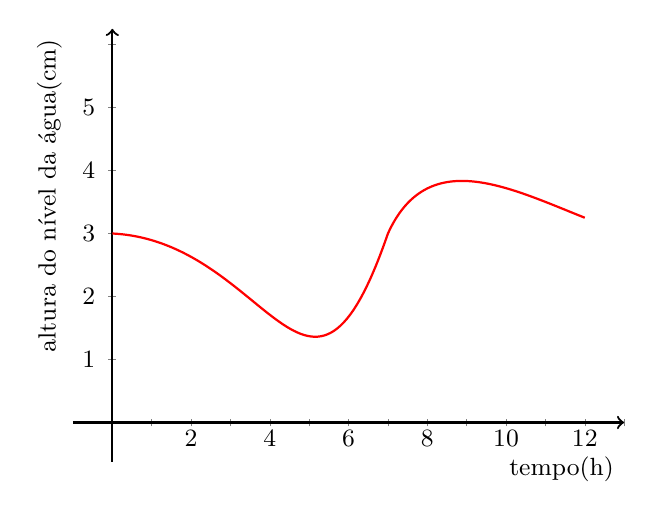
\begin{tikzpicture}
\draw[help lines, gray](0,-.05)grid[xstep=.5](6.5,.05);
\draw[help lines, gray](-.05,0)grid[ystep=.8](.05,5);
\draw[->,  thick](-.5,0)--(6.5,0)node[yshift=-.3cm,below left]{\small tempo(h)};
\draw[->,  thick](0,-0.5)--(0,5)node[left,xshift=-.8cm,rotate=90]{\small altura do nível da água(cm)};
\foreach \x in {2, 4, 6, 8, 10, 12}
\draw(.5*\x,-.2)node{\small \x};
\foreach \x in {1, 2, 3, 4, 5}
\draw(-.3,.8*\x)node{\small \x};
\draw [red,thick,smooth](0,2.4) .. controls (2,2.3)and(2.5,-.5) .. (3.5,2.4)
      (3.5,2.4) .. controls (4,3.5) and (5,3) .. (6,2.6);
\end{tikzpicture}\end{center}

\item Garrafas de água potável são vendidas em vários tamanhos e preços. Cada ponto no gráfico abaixo representa uma garrafa de água.
\begin{center}\begin{tikzpicture}[scale=1.5]
\draw[help lines,xstep=.5cm,ystep=.5cm](0,0)grid(4.7,2.3);
\draw[thick, ->](0,0)--(4.7,0);
\draw[thick, ->](0,0)--(0,2.3);
\draw(3.9,-.2) node {quantidade de \'{a}gua};
\draw(-.15,2) node[rotate=90]{pre\c{c}o};
\draw[fill=\currentcolor!80](1.5,1) circle (1pt) node[above left] {$A$};
\draw[fill=\currentcolor!80](3.5,2) circle (1pt) node[above left] {$B$};
\draw[fill=\currentcolor!80](.5,.5) circle (1pt) node[above left] {$C$};
\draw[fill=\currentcolor!80](4.5,1.5) circle (1pt) node[above left] {$D$};
\draw[fill=\currentcolor!80](3.5,1) circle (1pt) node[above left] {$E$};
\end{tikzpicture}\end{center}\begin{enumerate}
\item {} 
Qual garrafa armazena a maior quantidade de água?

\item {} 
Qual garrafa é vendida pelo preço mais alto?

\item {} 
Identifique dois pontos que estejam sobre uma mesma reta paralela ao eixo das abscissas (reta horizontal) e interprete o que isso significa.

\item {} 
Identifique dois pontos que estejam sobre uma mesma reta paralela ao eixo das ordenadas (reta vertical) e interprete o que isso significa.

\item {} 
Entre as garrafas \(A\) e \(E\), qual tem o melhor custo-benefício? Por que? E entre \(B\) e \(E\)? Por que?

\end{enumerate}
\end{enumerate}



% \ifnum \aluno=1
\renewcommand\chapterillustration{abertura-afim}
\else
\renewcommand\chapterillustration{abertura-afim-professor}
\fi
\renewcommand\chapterwhat{Funções linear e afim e suas representações algébrica e gráfica, taxa de variação, proporcionalidade direta, funções afins de domínio discreto (Progressões Aritméticas), Aplicações.}
\renewcommand\chapterbecause{O modelo de variação constante é um dos modelos mais presentes em observações científicas e até mesmo em nosso cotidiano. Ele pode ser identificado por exemplo, em relações que modelam a compra/consumo e venda, o esvaziamento de um recipiente por um ralo em função do tempo ou na relação entre distância e tempo do “movimento uniforme” estudado pela Cinemática, entre tantos outros. Um caso particularmente importante é aquele em que há proporcionalidade entre as grandezas envolvidas na modelagem. As ide ias desenvolvidas neste capítulo servem como base para aplicações em diversas áreas.}
\chapter{Função afim}



\mbox{}\thispagestyle{empty}\clearpage

\thispagestyle{empty}

\begin{center}
Projeto: LIVRO ABERTO DE MATEMÁTICA

\noindent \begin{tabular}{lcccr}
\includegraphics[scale=.15]{impa}& \quad\quad& \includegraphics[width=3cm]{logo} & \quad\quad& \includegraphics[scale=.24]{obmep} 
\end{tabular}
\end{center}

\vspace*{.3cm}

Cadastre-se como colaborador no site do projeto: \url{umlivroaberto.org}

Versão digital do capítulo:

\url{https://www.umlivroaberto.org/BookCloud/Volume_1/master/view/AF107.html}


\begin{tabular}{p{.15\textwidth}p{.7\textwidth}}
Título: & Função Afim\\
\\
Ano/ Versão: & 2020 / versão 1.2 de 27 de novembro de 2020\\
\\
Editora & Instituto Nacional de Matem\'atica Pura e Aplicada (IMPA-OS)\\
\\
Realização:& Olimp\'iada Brasileira de Matem\'atica das Escolas P\'ublicas (OBMEP)\\
\\
Produção:& Associação Livro Aberto\\
\\
Coordenação:& Fabio Simas, \\
            & Augusto Teixeira (livroaberto@impa.br)\\
\\
  Autores: & Gladson Antunes (UNIRIO),\\
        & Michel Cambrainha (UNIRIO),\\
             & Bruno Vianna (Colégio Pedro II).\\
\\
Revisão: &  Cydara Ripoll  \\
         &  Letícia Rangel \\
\\
Design: & Andreza Moreira (Tangentes Design) \\
\\
  Ilustrações: & Miller  Guglielmo \\ 
\\
Gráficos: & Beatriz Cabral e Tarso Caldas (Licenciandos da UNIRIO)\\
\\
  Capa: & Foto de Scott Webb, no Unplash \\
        & https://unsplash.com/photos/fMUIVein7Ng \\

\end{tabular}



\begin{figure}[b]
\begin{minipage}[l]{5cm}
\centering

{\large Licença:}

  \includegraphics[width=3.5cm]{cc-by-sa1}
\end{minipage}\hfill
\begin{minipage}[c]{5cm}
\centering
{\large Desenvolvido por}

\includegraphics[width=2.5cm]{logo-associacao.jpg}
\end{minipage}
\begin{minipage}[r]{5cm}
\centering

{\large Patrocínio:}
  \vspace{1em}
  \includegraphics[width=3.5cm]{itau}
\end{minipage}
\end{figure}

\mainmatter

\begin{apresentacao}{Introdução}

\subsection{Habilidades e pré-requsitos}

Neste capítulo contemplam-se as seguintes habilidades da segunda versão da \href{http://historiadabncc.mec.gov.br/documentos/bncc-2versao.revista.pdf}{Base Nacional Comum Curricular (BNCC):}

\begin{habilities}{EM11MT07}

Reconhecer função afim e suas representações algébrica e gráfica, identificar o modelo de variação e a taxa de variação, incluindo os casos em que a variação é proporcional (linear), e utilizar essas noções para representar e resolver problemas como os de Movimento Uniforme, entre outros.
\end{habilities}

Os pré-requisitos para este capítulo são:

\begin{habilities}{EF07MA13} Resolver e elaborar problemas que envolvam variação de proporcionalidade direta e de proporcionalidade inversa entre duas grandezas, utilizando sentença algébrica para expressar a relação entre elas.

\tcbsubtitle{EF07MA14} Resolver e elaborar problemas que possam ser representados por equações polinomiais de 1º grau, redutíveis à forma \(ax+b=c\), fazendo uso das propriedades da igualdade.
\end{habilities}

Além disso há outras habilidades que se relacionam com os conceitos abordados nesse capítulo, a saber,

\begin{habilities}{EF09MA05} Resolver e elaborar problemas que envolvam porcentagens, com a ideia de aplicação de percentuais sucessivos e a determinação das taxas percentuais, preferencialmente com o uso de tecnologias digitais, no contexto da educação financeira.

\tcbsubtitle{EF09MA07} Resolver problemas que envolvam a razão entre duas grandezas de espécies diferentes, como velocidade e densidade demográfica.

\tcbsubtitle{EF09MA08} Resolver e elaborar problemas que envolvam relações de proporcionalidade direta e inversa entre duas ou mais grandezas, inclusive escalas, divisão em partes proporcionais e taxa de variação, em contextos socioculturais, ambientais e de outras áreas.

\end{habilities}

Prezado colega, o presente capítulo foi concebido a partir de uma abordagem de função afim não usual. Deixamos a cargo do aluno levantar conjecturas a respeito dos conceitos, definições e propriedades da função afim. Essas conjecturas ou indagações são provocadas por meio de atividades que abordam os conceitos a serem trabalhados.
\columnbreak

Iniciamos o capítulo resgatando a ideia de grandezas proporcionais e relacionando-a com o conceito de função linear. É comum que a noção de proporcionalidade, mais especificamente a de proporcionalidade direta, amplamente vinculada à “regra de três”, seja associada pelos estudantes a qualquer variação entre grandezas. Ainda que, de fato, a proporcionalidade tenha um papel de destaque em modelos da física e da química, nem toda variação entre grandezas é um modelo desse tipo. Portanto acreditamos que, na condução das atividades seja natural para o professor (e recomendamos que o faça) chamar a atenção dos estudantes para o fato que existem grandezas cuja relação não é de proporcionalidade.

Busque com seus estudantes desenvolver as atividades, de maneira a deixá-los livres para criar conjecturas ou até mesmo a chegar a conclusões, por meio de argumentos diversos, sejam eles visuais, geométricos, algébricos, lógicos ou até mesmo dissertativos.

Vale ressaltar alguns pontos:
\begin{itemize}
\item {} 
Boa parte das atividades tem como objetivo apontar para os estudantes a importância da análise da taxa de variação para inferirmos se uma função é afim ou não. Neste capítulo, resolvemos não fazer uso do termo \textbf{coeficiente angular} da reta. Essa decisão se pauta em dois aspectos: (i) Dependendo da escolha da unidade para as grandezas envolvidas, a imagem da representação gráfica pode sugerir um ângulo cuja a tangente não correspnde ao coeficiente angular da reta determinada pela função, e assim levar ao equívoco. (ii) Além disso, acreditamos que a compreensão de taxa de variação pode ser mais fácil se dotada de significado. Assim, por exemplo, é mais fácil compreender a taxa de variação entre temperatura e altitude ou entre velocidade e tempo do que associar essa ideia a um conceito essencialmente numérico, que é o caso do coeficiente angular de uma reta. O ângulo tem apelo visual independente das escalas escolhidas para os eixos, e assim, chamar a taxa de variação de coeficiente angular pode trazer confusão. Portanto, neste texto, optamos por destacar a especificidade de cada conceito associando o termo taxa de variação à função afim e coeficiente angular a retas (desde que estejam em um sistema de coordenadas cujos eixos apresentam-se na mesma escala).

\clearpage
\item {} 
Também não achamos adequado o termo \emph{coeficiente linear} para o \(b\) em \(f(x)=ax+b\). Primeiramente porque, quando ele é não nulo a função deixa de ser “linear”, então ele funciona mais como uma medida da “não-linearidade” da função. Em alguns livros ele também é chamado de \emph{intercepto}. Também optamos por não utilizar essa nomenclatura por ela ser restringir apenas aos casos em que os eixos estão na posição tradicional (isto é, se cruzando no \((0,0)\)) e além disso, \(0\) deve pertencer ao domínio da função em questão. Por essas razões, resolvemos não dar um nome para o “\(b\)”, apenas lhe dar um significado geométrico que serve em qualquer situação: a medida da translação vertical que se faz no gráfico da função linear \(\ell(x)=ax\) para se obter o gráfico da função \(f(x)=ax+b\).

\item {} 
Em alguns livros o capítulo tem o nome de “Função do 1° grau”. Também acreditamos que esse termo é equivocado pois função não tem grau, o que tem grau é polinômio. No entanto, podemos dizer que toda função afim pode ser expressa por um polinômio do 1° grau.

\item {} 
Também é comum, apresentarmos uma função afim da forma \(f(x)=ax+b\), sem nos preocuparmos se o seu domínio é toda real ou não. Algumas atividades abordam funções com domínios discretos, outras cujos domínios são intervalos reais. Sendo assim, ressalte para seus estudantes a importância do domínio da função, como por exemplo: \(f:\mathbb{R}\to\mathbb{R}\) onde \(f(x)=2x+1\) ; \(g:[0,2]\to \mathbb{R}\) onde \(g(x) = -2x\)   e  \(h:\mathbb{N}\to\mathbb{R}\) onde \(h(n)=3n-5\); de maneira que o gráfico de \(f\) é uma reta; de \(g\) é um segmento de reta e de \(h\) é um conjunto de pontos colineares.

\item {} 
Pode ocorrer que algum estudante tente associar uma reta de inclinação negativa a uma relação de proporcionalidade inversa. Caso essa questão seja levantada durante a execução das atividades, mostre a seus estudantes, com um exemplo simples, como é a curva que representa a variação de proporcionalidade inversa (hipérbole). Decidimos não discutir esse assunto nesse capítulo para que não ficasse demasiadamente extenso.

\item {} 
Sempre que possível, utilize recursos computacionais para desenvolver o discutir as atividades propostas ou para gerar novas atividades. Isso torna o estudo mais dinâmico.  São propostas duas atividades que apresentam versões digitais criadas no Geogebra. Caso não consiga trabalhá-las em sala de aula, estimule seus estudantes a acessarem os respectivos links.

\item {} 
As habilidades que estão listadas como pré-requisitos são retomadas pelas atividades e eventualmente aprofundadas em relação à maneira como elas são tradicionalmente exploradas no Ensino Fundamental.

\end{itemize}

\textbf{Alguns distratores} (apontados pela literatura de pesquisa)
\begin{itemize}
\item {} 
A repetida confirmação da validade da proporcionalidade - juntamente com o status intuitivo que o conceito recebe gradualmente - pode conduzir a uma ideia errada: se houver uma relação entre duas variáveis, essa relação provavelmente é proporcional. Estudos mostram que existe uma tendência generalizada entre os estudantes americanos com idade de \(12\) a \(16\) anos de que, se uma figura aumentar de \(k\) vezes, a área e o volume dessa figura serão ampliados também de \(k\) vezes. \citep{Dooren-et-al-2005}

\item {} 
A pesquisa tem documentado dificuldades dos estudantes com o conceito de inclinação. Há confusões associadas ao cálculo da inclinação e à interpretação de funções lineares e seus gráficos. Os estudantes também apresentam dificuldades em relacionar gráficos a equações lineares e à noção de taxa de variação. Eles têm dificuldade em perceber a inclinação como uma razão e conectar tal razão ao modelo físico. \citep{Stump-1999}

\item {} 
Nem toda razão pode ser expressa por números racionais, o que vincula, por meio da proporcionalidade, a apresentação dos números irracionais. Isso sinaliza que nem todas as situações podem ser resolvidas recorrendo-se apenas aos números racionais. \citep{Silva-et-al-2013}

\end{itemize}
\end{apresentacao}

\def\currentcolor{session1}
\clearmargin
\begin{objectives}{Na piscina}
{
\begin{itemize}
\item Reconhecer uma relação de proporcionalidade entre grandezas a partir da análise gráfica e da construção e análise dos dados em uma tabela;

\item Conjecturar sobre a representação gráfica de grandezas diretamente proporcionais, associando-a a um conjunto de pontos colineares
\end{itemize}
}{1}{2}
\end{objectives}
\begin{sugestions}{Na piscina}
{
\begin{itemize}
\item Como primeira atividade do capítulo, priorize as ideias em detrimento do rigor matemático. Ajude seus estudantes a transcreverem suas ideias de maneira precisa, ainda que informais.
No item (b), podem surgir respostas como: a primeira coluna aumenta de “uma em uma hora” enquanto a segunda aumenta de “200 em 200 litros”; a segunda coluna é obtida multiplicando a primeira por 200; tabela gerada pela função f(n)=200⋅n com domínio {0,1,2,3,4,5}. Apesar de não serem consequências diretas da definição, estão corretas e serão tratadas ao longo do capítulo.
\end{itemize}
}{1}{2}
\end{sugestions}
\clearmargin
\begin{answer}{Na piscina}
{
\begin{enumerate}
\item Piscina 1

\adjustbox{valign=t}
{
\begin{tabu} to \textwidth{|c|c|}
\hline
\thead
Tempo ($h$) & volume (litros) \\
\hline
0 & 0 \\
\hline
1 & 200 \\
\hline
2 & 400 \\
\hline
3 & 600 \\
\hline
4 & 800 \\
\hline
5 & 1000 \\
\hline
\end{tabu}
}

\vspace{2em}

Piscina 2

\adjustbox{valign=t}
{
\begin{tabu} to \textwidth{|c|c|}
\hline
\thead
Tempo ($h$) & volume (litros) \\
\hline
0 & 0 \\
\hline
1 & 150 \\
\hline
2 & 200 \\
\hline
3 & 300 \\
\hline
4 & 500 \\
\hline
5 & 800 \\
\hline
6 & 900 \\
\hline 
7 & 950 \\
\hline
8 & 1000 \\
\hline
\end{tabu}
}

\vspace{2em}


\item Sim, pois para $k\in\{0,2,3,4,5\}$ tempo
\[\begin{array}{ccc}
x\quad &\overline{\quad \quad \quad}& \quad y \\
k\cdot 1 \quad &\overline{\quad \quad \quad}& \quad k\cdot 200
\end{array}\]

\item Não, pois ao final da primeira hora o volume total de água aumentou 150 litros e na hora seguinte aumentou apenas 50 litros. Para haver proporcionalidade direta, deveria ter aumentado também 150 litros na segunda hora, totalizando 300 litros.
\end{enumerate}
}{1}
\end{answer}
\begin{sugestions}{Para refletir}
{
  Este é um convite à uma primeira reflexão sobre as propriedades geométricas de pontos colineares e sua relação com grandezas proporcionais. Conduza os seus estudantes a fazerem conjecturas sobre como deve ser a representação gráfica de grandezas diretamente proporcionais.
}{1}{1}
\end{sugestions}
\explore{Função Linear}\label{funcaolinear}
No capítulo de Funções, você foi apresentado ao conceito de função, uma relação entre duas grandezas que atende determinadas condições. Neste capítulo, pretendemos colocá-lo em contato com um dos modelos mais presentes em observações científicas e até mesmo em nosso cotidiano, o modelo de variação constante, aqui representado pelo conceito de função afim. Este modelo pode ser identificado por exemplo, em relações que modelam a compra/consumo e venda, o esvaziamento de um recipiente por um ralo em função do tempo ou na relação entre distância e tempo do “movimento uniforme” estudado pela Cinemática, entre tantos outros. Antes de estudarmos a função afim propriamente dita, vamos entender um de seus casos particulares, a função linear.

Comecemos analisando os seguintes problemas:

\begin{figure}[H]
\centering
\noindent\includegraphics[width=400bp]{naoprop.png}
\end{figure}


Os três problemas acima fornecem três informações e propõem que, a partir delas, determinemos uma quarta informação. Esse é o enunciado típico de problemas cujo método de solução é conhecido como “regra de três”. Entretanto, nenhum dos problemas apresentados, como você deve ter percebido, pode ser resolvido aplicando a tal regra. Você consegue imaginar por quê?

Isso se deve ao fato de que as grandezas relacionadas não são proporcionais entre si. Não é verdade que se \(5\) músicos tocam uma peça de música em \(10\) minutos, \(35\) músicos (que é \(7 \times 5\)) tocarão a peça em \(7 \times 10\) minutos, afinal trata-se da mesma música, logo \(35\), \(45\) ou \(179\) músicos tocarão a tal peça nos mesmos \(10\) minutos. Isto é, o tempo de execução não é diretamente proporcional ao número de músicos que executam a música.

\begin{description}
\item[Teorema]
\leavevmode\phantomsection\label{\detokenize{AF107-0:term-grandezas-diretamente-proporcionais}}
Diz-se que \textbf{duas grandezas são diretamente proporcionais} quando elas se correspondem de tal modo que, multiplicando-se uma quantidade de uma delas por um número real, a quantidade correspondente da outra fica multiplicada pelo mesmo número, sempre que os resultados dessas multiplicações fizerem sentido no contexto observado.
\[\begin{array}{ccc}
X\quad &\overline{\quad \quad \quad}& \quad Y \\
k\cdot X \quad &\overline{\quad \quad \quad}& \quad k\cdot Y
\end{array}\]
\end{description}

É muito comum encontrarmos situações no nosso dia a dia em que as grandezas envolvidas são diretamente proporcionais, e você certamente já resolveu muitos problemas, na escola e fora dela, usando a “regra de três”.

\begin{task}{Na piscina}
\label{ativ-na-piscina}

Duas piscinas de 1000 litros cada estão sendo enchidas simultaneamente. A piscina 1 leva 5 horas para ficar completamente cheia e a piscina 2, 8 horas. A cada hora, o volume total de água em cada piscina foi sendo registrado em dois gráficos


\begin{figure}[H]
\centering

\begin{tikzpicture}[scale=1.5, every node/.style={scale=1}]
\tikzstyle{ponto}=[circle, minimum size=3pt, inner sep=0, draw=\currentcolor!80, fill=\currentcolor!80, shift only]
\begin{scope}[yscale=.5]
\draw[lightgray](0,0)grid[xstep=.25,ystep=.25](6,10);
\draw[gray](0,0)grid(6,10);
\draw[thick, ->](0,0)--(6,0)node [below, shift={(-0.55,-0.2)}]{tempo(horas)};
\draw[thick, ->](-0,0)--(0,10);
\node[right, rotate=90]at (-.9,6){capacidade(litros)};
\foreach \x in{0,1, 2, 3, 4, 5}
\node[ponto]at(\x,2*\x){};
\foreach\x in{0,1, 2, 3, 4, 5, 6}
\node[below] at(\x, 0){ \x};
\foreach\y in{100, 200, 300, ..., 1000}
\node[left]at(0,.01*\y){ \y};
\end{scope}
\end{tikzpicture}
\caption{Piscina 1}
\label{piscina1}
\end{figure}
\begin{figure}[H]
\centering

\begin{tikzpicture}[scale=1.5, every node/.style={scale=1}]
\tikzstyle{ponto}=[circle, minimum size=3pt, inner sep=0, draw=\currentcolor!80, fill=\currentcolor!80, shift only]
\begin{scope}[yscale=.5]
\draw[lightgray](0,0)grid[xstep=.25,ystep=.25](8,10);
\draw[gray](0,0)grid(8,10);
\draw[thick, ->](0,0)--(8,0)node [below, shift={(-0.55,-0.3)}]{tempo(horas)};
\draw[thick, ->](-0,0)--(0,10);
\node[right, rotate=90]at (-.9,6){ capacidade(litros)};
\node[ponto]at(0,0){};
\node[ponto]at(1,1.5){};
\node[ponto]at(2,2){};
\node[ponto]at(3,3){};
\node[ponto]at(4,5){};
\node[ponto]at(5,8){};
\node[ponto]at(6,9){};
\node[ponto]at(7,9.5){};
\node[ponto]at(8,10){};
\foreach\x in{0,1, 2, 3, 4, 5, 6, 7, 8}
\node[below] at(\x, 0){\x};
\foreach\y in{100, 200, 300, ..., 1000}
\node[left]at(0,.01*\y){\y};
\end{scope}
\end{tikzpicture}
\caption{Piscina 2}
\label{piscina2}

\end{figure}

\begin{enumerate}
\item {} 
Construa uma tabela com os dados de cada gráfico.

\item {} 
As grandezas volume total de água e tempo de enchimento da piscina 1 são diretamente proporcionais? Explique.

\item {} 
As grandezas volume total de água e tempo de enchimento da piscina 2 são diretamente proporcionais? Explique.

\end{enumerate}
\end{task}

\begin{reflection}

Suponha que os dados numéricos fossem omitidos dos eixos nos dois gráficos. Ainda assim seria possível determinar a proporcionalidade ou não entre as grandezas? Como?
\end{reflection}

\clearpage
\def\currentcolor{session4}
\begin{sugestions}{Para refletir}
{
  Até o presente momento, apenas argumentamos que se duas grandezas são proporcionais então elas se relacionam de maneira que uma delas é uma função linear da outra. Essa reflexão vai no sentido da afirmação recíproca. E ainda faz uma provocação, sem ter o intuito de formalizar, no sentido de intuir que a função inversa de uma função linear é também uma função linear.
}{1}{2}
\end{sugestions}

\arrange{Função Linear}
\label{\detokenize{AF107-1::doc}}\label{\detokenize{AF107-1:organizando-as-ideias-funcao-linear}}
Considere duas grandezas diretamente proporcionais que podem assumir quaisquer valores reais e vamos representá-las pelas letras \(x\) e \(y\). Então, sempre que multiplicarmos \(x\) por qualquer número real \(k\), o valor correspondente da grandeza \(y\) também fica multiplicado pelo mesmo valor. Isto é
\[\begin{array}{ccc}
x\quad &\overline{\quad \quad \quad}& \quad y \\
k\cdot x \quad &\overline{\quad \quad \quad}& \quad k\cdot y
  \end{array}\]
Vamos agora, traduzir a propriedade acima para a linguagem de função. Consideremos que a grandeza \(y\) é expressa como função da grandeza \(x\), isto é, \(y=f(x)\). Vamos supor que quando a variável $x$ vale 1, o valor correspondente de $y$ é $a$, ou seja, $f(1)=a$. Assim, teremos

\[\begin{array}{ccc}
x\quad &\overline{\quad \quad \quad}& \quad f(x) \\
1 \quad &\overline{\quad \quad \quad}& \quad a \\
2 \quad &\overline{\quad \quad \quad}& \quad 2a \\
3 \quad &\overline{\quad \quad \quad}& \quad 3a \\
\vdots \quad &\overline{\quad \quad \quad}& \quad \vdots\\
  \end{array}\]

\begin{observation}{}
Usando a ``regra de três'' nas duas primeiras linhas fica assim
\[\begin{array}{ccc}
x \quad &\overline{\quad \quad \quad}& \quad f(x)\\
1\quad &\overline{\quad \quad \quad}& \quad a \end{array}\]
O que nos leva a
\[\dfrac x1 = \dfrac {f(x)}a \Longrightarrow f(x) = a\cdot x\]
\end{observation}

Toda função real que pode ser expressa na forma $f(x)=ax$ para algum número real $a$, é chamada de \textbf{função linear}. Neste caso, as grandezas representadas pelas variáveis $x$ e $y=f(x)$ são diretamente proporcionais. O número $a=f(1)$ é chamado de \textbf{constante de proporcionalidade} entre as grandezas.


Na \DUrole{xref,std,std-ref}{Atividade Na piscina} você deve ter percebido que as grandezas relacionadas eram diretamente proporcionais apenas no caso da piscina 1. Naquele caso, a função que fornece o volume de água na piscina em função do tempo é dada por \(V:\{1,2,3,4,5\}\to \mathbb{R}\),   \(V(t)=V(1)\cdot t=200\cdot t\).

\begin{reflection}

Suponha que duas grandezas \(x\) e \(y\) se relacionem de maneira que \(y\) seja uma função linear de \(x\).
\begin{enumerate}
\item {} 
Essas duas grandezas são proporcionais?

\item {} 
Podemos afirmar também que \(x\) é uma função linear de \(y\)?

\end{enumerate}
\end{reflection}

\needspace{.2\textheight}
\def\currentcolor{session2}
\begin{objectives}{Taxa de Câmbio}
{
\begin{itemize}
\item Utilizar a taxa de câmbio fornecida para realizar a conversão do valor dado em moeda estrangeira para o valor correspondente em reais.

\item Obter a partir das informações fornecidas a função linear que converte dólar americano em reais.

\end{itemize}
}{1}{1}
\end{objectives}
\begin{sugestions}{Taxa de Câmbio}
{
\begin{itemize}
\item É bastante provável que no item \titem{c)} os estudantes apresentem o seguinte raciocínio: se 1 dólar americano equivale a R\$ $3{,}20$ reais então $x$ dólares americanos irão corresponder a $y$ reais, isto é, $y=3,20\cdot x$. Em analogia ao que foi feito anteriormente, é importante chamar atenção de que se $y=f(x)$ é a função que fornece a quantia equivalente em reais a x dólares americanos, como as grandezas envolvidas são diretamente proporcionais e $f(1)=3{,}20$, então $f(x)=x\cdot f(1)$ e portanto $f(x)=3{,}20{,}x$.

\item Ainda no item \titem{c)} o questionamente apresentado sobre o domínio da função tem como objetivo levar a uma reflexão de que na prática não faz sentido, por exemplo, converter $\sqrt{5}$ dólares americanaos para reais.
\end{itemize}
}{1}{1}
\end{sugestions}
\begin{answer}{Taxa de Câmbio}
{
\begin{enumerate}

\item A partir da taxa de câmbio fornecida sabemos que 1 dólar americano é equivalente a R\$ $320{,}00$, e portanto, para comprar 100 dólares americanos serão necessários R\$ $320{,}00$. \si{kg}

\item Como nesse dia 1 euro é equivalente a R\$ $4{,}00$, então será necessário desembolsar R\$ $800{,}00$ para a compra de $200$ euros.

\item Vamos chamar de $y=f(x)$ a função que fornece a quantia equivalente em reais a x dólares americanos. Como as grandezas envolvidas são diretamente proporcionais e $f(1)=3{,}20$ (veja que isso é a tradução, usando a linguagem de função, de que 1 dólar americano equivale a R\$ $3{,}20$), então $f(x)=x\cdot f(1)$ e portanto $f(x)=3{,}20\cdot x$. Como na prática não existem quantias irracionais de dólares americanos e de reais, devemos considerar $f:\Q\rightarrow\Q$.

\item Utilizando a função obtida no item anterior vemos que R\$ $2000,00$ equivalem a $x\displaystyle=\frac{2000}{3}{,}20=625$ reais. Raciocinando de forma análoga obtemos que com R\$ $2000{,}00$ poderão ser adquiridos $\displaystyle\frac{2000}{4}=500$ euros.
\end{enumerate}
}{0}
\end{answer}
\begin{objectives}{Proporcionalidade na construção de retângulos}
{
\begin{itemize}
\item Levar o estudante a relacionar os conceitos de proporcionalidade e semelhança de figuras e função linear.

\item Construir retângulos que sejam semelhantes a um retângulo dado.

\end{itemize}
}{1}{1}
\end{objectives}
\clearmargin
\marginpar{\vspace{.5em}}
\begin{answer}{Proporcionalidade na construção de retângulos}
{
\begin{enumerate}
\item Não, pois a medida da base dobrou e a altura se manteve.

\item $3$, pois se a medida da base dobrou a altura deve dobrar $1{,}5\cdot2=3$. Os retângulos se relacionam por meio da função linear $f(x)=2\cdot x$.

\item $2{,}5$, pois em todos os retângulos a razão de semelhança, entre a base e a altura é de $12$, portando a altura deve ser a metade da base. Neste caso os retângulos se relacionam por meio da função linear $f(x)=53\cdot x$.

\item $8$, pelo mesmo motivo citado anteriormente, a base deve ser o dobro a altura.

\item Não, pois a razão entre base e altura não é de $12$.

\item $\sqrt{33}$, pois a altura de um triângulo equilátero de lado $3$ é $\frac{3\sqrt{33}}{2}$, ao assumir essa medida como altura do retângulo, sua base deve ser o dobro dessa medida.

\end{enumerate}
}{1}
\end{answer}
\clearmargin
\begin{objectives}{Qual é a área?}
{
\begin{itemize}
\item Em um círculo dado, reconhecer a relação de dependência entre a medida do ângulo central e a medida da área do setor circular.

\item Inferir que a medida da área do setor é diretamente proporcional a medida do ângulo central.

\item Determinar a medida da área do setor circular dada a medida do ângulo central e vice-versa.

\end{itemize}
}{1}{1}
\end{objectives}
\marginpar{\vspace{-1em}}
\begin{sugestions}{Qual é a área?}
{
\begin{itemize}
\item Nos dois primeiros itens procure incentivar os alunos a resolver o problema utilizando apenas processos mentais, ou ao menos na hora de discutir a solução, utilize argumentações que valorizem a estimativa, tais como:

\begin{itemize}
\item Como $\frac{1}{4}$ de $20$ é $5$, e $14$ é um valor um pouco menor que $34$ de $20$ então o setor circular de área $14$ tem que ser menor do que $34$ do círculo.

\item Ao analisar as opções descartamos a opção “2” por ser uma região menor que $34$ da área do círculo, descartamos também a opção “3” por se tratar de um valor entre $15$ e $20$ mais próximo de $15$, logo a resposta correta está representada pela opção “1”.
\end{itemize}

\item Nos itens \titem{c)} e \titem{d)}, discuta com a turma a importância de ter sido apresentado a medida do ângulo.
\end{itemize}
}{1}{1}
\end{sugestions}
\begin{answer}{Qual é a área?}
{
\begin{enumerate}\setcounter{enumi}{4}
\item 2)
\item 1)
\item Uma possível resposta seria: sendo a área total do círculo igual a $20$, então $14$ do círculo equivale a uma área 5. No entanto, como as áreas destacadas nos itens apresentados estão muito próximas esse critério não nos permite concluir com exatidão qual seria a resposta correta, que no caso é o item 2).
\item 2)
\end{enumerate}
}{1}
\end{answer}
\clearmargin
\begin{answer}{Qual é a área}
{
  \begin{enumerate}
  \item Fazendo uma regra de três, item 1).
  \item $S:[0,360]\rightarrow\R$ em que $S(x)=\frac{x}{18}$
  \end{enumerate}
}{1}
\end{answer}

\practice{Função Linear}
\label{\detokenize{AF107-1:praticando}}

\begin{task}{Taxa de câmbio}
\label{ativ-cambio}



Segundo o \href{http://www.bcb.gov.br/pre/bc\_atende/port/taxCam.asp}{site do Banco Central do Brasil}, a \emph{taxa de câmbio} é o preço de uma moeda estrangeira medido em unidades ou frações (centavos) da moeda nacional. Em um determinado dia as taxas de câmbio do dólar americano e do euro eram respectivamente R\$ $3{,}20$ e R\$ $4{,}00$.
\begin{enumerate}
\item {} 
Nesse mesmo dia você deseja comprar \(100\) dólares. Qual seria o valor em reais necessário para realizar essa compra?

\item {} 
Para adquirir nesse mesmo dia \(200\) euros, qual o valor em reais deverá ser desembolsado?

\item {} 
A partir da taxa praticada nesse dia, apresente uma função que converta dólar americano para reais. Qual o conjunto domínio mais adequado a ser considerado para essa função? Justifique.

\item {} 
Com a taxa de câmbio que está sendo praticada nesse dia, quantos dólares americanos podem ser comprados com R\$ $2000{,}00$. Com os mesmos R\$ $2000{,}00$, quantos euros podem ser adquiridos?

\end{enumerate}
\end{task}



\begin{task}{Proporcionalidade na construção de retângulos}
\label{ativ-prop-retangulo}

Considere o retângulo \(R\) abaixo, de lados \(3\) e \(1{,}5\), e responda as questões propostas.

\begin{figure}[H]
\centering

\begin{tikzpicture}
\tikzstyle{ponto}=[circle, minimum size=2pt, inner sep=0, draw=black, fill=black, shift only]
\draw[thick,black,fill=\currentcolor!80] (0.,0.) -- (3.,0.) -- (3.,1.5) -- (0.,1.5) -- cycle;
\draw (0.2,0.) -- (0.2,0.2) -- (0.,0.2) -- (0.,0.);
\draw (0.,1.3) -- (0.2,1.3) -- (0.2,1.5) -- (0.,1.5);
\draw (2.8,1.5) -- (2.8,1.3) -- (3.,1.3) -- (3.,1.5);
\draw(3.,0.2) -- (2.8,0.2) -- (2.8,0.) -- (3.,0.);
\node[ponto]at(0,0){};
\node[ponto]at(3,0){};
\node[ponto]at(3,1.5){};
\node[ponto]at(0,1.5){};
\node[below ]at(0,0){$$};
\node[below ]at(3,0){$$};
\node[above ]at(3,1.5){$$};
\node[above ]at(0,1.5){$$};
\node[above]at(1.7,-.7){$3$};
\node[right]at(3,.75){$1{,}5$};
\end{tikzpicture}

\end{figure}

\begin{enumerate}
\item {} 
Observe o retângulo da figura a seguir e determine se ele é semelhante ou não ao retângulo \(R\).

\begin{figure}[H]
\centering

\begin{tikzpicture}
\tikzstyle{ponto}=[circle, minimum size=2pt, inner sep=0, draw=black, fill=black, shift only]
\draw[thick,black,fill=\currentcolor!80] (0.,0.) -- (6.,0.) -- (6.,1) -- (0.,1.)-- cycle;
\draw (0.2,0.) -- (0.2,0.2) -- (0.,0.2) -- (0.,0.);
\draw (0.,.8) -- (0.2,.8) -- (0.2,1) -- (0.,1);
\draw (5.8,1) -- (5.8,.8) -- (6.,.8) -- (6.,1);
\draw(6.,0.2) -- (5.8,0.2) -- (5.8,0.) -- (6.,0.);
\node[ponto]at(0,0){};
\node[ponto]at(6,0){};
\node[ponto]at(6,1){};
\node[ponto]at(0,1){};
\node[below ]at(0,0){$$};
\node[below ]at(6,0){$$};
\node[above ]at(6,1){$$};
\node[above ]at(0,1){$$};
\node[above]at(3,-.7){$6$};
\node[right]at(6,.5){$1{,}5$};
\end{tikzpicture}

\end{figure}

\item {} 
Na figura a seguir temos a medida base de um retângulo em destaque, qual deve ser a medida de sua altura para que o retângulo gerado seja semelhante a \(R\)? Qual a função linear que relaciona esses dois retângulos?

\begin{figure}[H]
\centering


\begin{tikzpicture}
\tikzstyle{ponto}=[circle, minimum size=2pt, inner sep=0, draw=black, fill=black, shift only]
\fill[bottom color=\currentcolor!80,top color =white] (0.,0.) -- (6.,0.) -- (6.,.5) -- (0.,.5) -- cycle;
\draw (0.2,0.) -- (0.2,0.2) -- (0.,0.2) -- (0.,0.);
\draw(6.,0.2) -- (5.8,0.2) -- (5.8,0.) -- (6.,0.);
\draw(0.,.5)--(0.,0.) -- (6.,0.) -- (6.,.5);
\node[ponto]at(0,0){};
\draw[fill](0,.6)circle(.5pt);
\draw[fill](0,.7)circle(.5pt);
\draw[fill](0,.8)circle(.5pt);
\node[ponto]at(6,0){};
\draw[fill](6,.6)circle(.5pt);
\draw[fill](6,.7)circle(.5pt);
\draw[fill](6,.8)circle(.5pt);
\node[below ]at(0,0){$$};
\node[below ]at(6,0){$$};
\node[above ]at(6,1.5){$$};
\node[above ]at(0,1.5){$$};
\node[above]at(3,-.7){$6$};
\end{tikzpicture}

\end{figure}
\item {} 
Seguindo a mesma ideia do item anterior, qual deve ser a medida da altura desse novo retângulo de base \(5\), para que ele seja semelhante a \(R\)? E neste caso, qual a função linear entre os retângulos?

\begin{figure}[H]
\centering


\begin{tikzpicture}
\tikzstyle{ponto}=[circle, minimum size=2pt, inner sep=0,   draw=black, fill=black, shift only]
\fill[bottom color=\currentcolor!80,top color =white] (0.,0.) -- (5.,0.) -- (5.,.5) -- (0.,.5) -- cycle;
\draw (0.2,0.) -- (0.2,0.2) -- (0.,0.2) -- (0.,0.);
\draw(5.,0.2) -- (4.8,0.2) -- (4.8,0.) -- (5.,0.);
\draw(0.,.5)--(0.,0.) -- (5.,0.) -- (5.,.5);
\node[ponto]at(0,0){};
\draw[fill](0,.6)circle(.5pt);
\draw[fill](0,.7)circle(.5pt);
\draw[fill](0,.8)circle(.5pt);
\node[ponto]at(5,0){};
\draw[fill](5,.6)circle(.5pt);
\draw[fill](5,.7)circle(.5pt);
\draw[fill](5,.8)circle(.5pt);
\node[below ]at(0,0){$$};
\node[below ]at(5,0){$$};
\node[above ]at(5,1.5){$$};
\node[above ]at(0,1.5){$$};
\node[above]at(2.5,-.7){$5$};
\end{tikzpicture}

\end{figure}
\item {} 
Já na figura a seguir, apresentamos um retângulo de altura \(4\), qual deve ser a medida da base desse novo retângulo, para que ele seja semelhante a \(R\)?

\begin{figure}[H]
\centering

\begin{tikzpicture}
\tikzstyle{ponto}=[circle, minimum size=2pt, inner sep=0, draw=black, fill=black, shift only]
\fill[left color = white, right color =\currentcolor!80,] (2.,0.) -- (3.,0.) -- (3.,2.5) -- (2.,2.5) -- cycle;
\draw[thick] (2.,0.) -- (3.,0.) -- (3.,2.5) -- (2.,2.5) ;
\draw (2.8,2.5) -- (2.8,2.3) -- (3.,2.3) -- (3.,2.5);
\draw(3.,0.2) -- (2.8,0.2) -- (2.8,0.) -- (3.,0.);
\node[ponto]at(0,0){};
\node[ponto]at(3,0){};
\node[ponto]at(3,2.5){};
\node[ponto]at(0,2.5){};
\node[below ]at(0,0){$$};
\node[below ]at(3,0){$$};
\node[above ]at(3,2.5){$$};
\node[above ]at(0,2.5){$$};
\node[right]at(3,1.25){$4$};
\draw[fill](1.7,0)circle(.5pt);
\draw[fill](1.8,0)circle(.5pt);
\draw[fill](1.9,0)circle(.5pt);
\draw[fill](1.7,2.5)circle(.5pt);
\draw[fill](1.8,2.5)circle(.5pt);
\draw[fill](1.9,2.5)circle(.5pt);
\end{tikzpicture}

\end{figure}
\item {} 
Na figura a seguir, apresentamos um retângulo cuja base tem a mesma medida da base de \(R\) (igual a \(3\)), e cuja altura coincide com a de um triângulo equilátero de lado medindo \(3\). Esse retângulo é semelhante a \(R\)?

\begin{figure}[H]
\centering


\begin{tikzpicture}
\tikzstyle{ponto}=[circle, minimum size=2pt, inner sep=0, draw=black, fill=black, shift only]
\draw[fill=\currentcolor!80,very thick](0,0)--(4,0)--(4,3.46)--(0,3.46)--cycle;
\draw[fill=terciario,very thick](0,0)--(4,0)--(2,3.46)--cycle;
\node[ponto]at(0,0){};
\node[ponto]at(4,0){};
\node[ponto]at(4,3.46){};
\node[ponto]at(0,3.46){};
\node[ponto]at(2,3.46){};
\node[below]at(0,0){$$};
\node[below]at(4,0){$$};
\node[above]at(4,3.46){$$};
\node[above]at(0,3.46){$$};
\node[above]at(2,3.46){$$};
\node[above]at(2,-.8){$3$};
\end{tikzpicture}

\end{figure}
\item {} 
Se utlizarmos a altura do retângulo da figura anterior na construção de um novo retângulo, qual deve ser a medida de sua base para que seja semelhante a \(R\)?

\end{enumerate}
\end{task}


\begin{task}{Qual é a área?}
\label{ativ-qual-area}

Caso tenha disponibilidade, sugerimos o uso da construção GeoGebra disponível \href{https://www.geogebra.org/m/Xjjym4e7}{neste link}, que é a versão eletrônica dessa atividade.

\begin{figure}[H]
\centering

\noindent\includegraphics[width=100bp]{{codigo}.png}
\end{figure}



\begin{enumerate}
\item {}
Cada círculo representado a seguir tem área total \(20\). Um   dos setores circulares destacados em verde nesses círculos tem área \(14\). Qual é esse setor?

\begin{figure}[H]
\centering


  \begin{tikzpicture}
    \draw(0,0)circle(1);
    \draw[fill=\currentcolor!80] (1,0)--(0,0) --(210:1) arc (210:0:1);
    \node at(-1,1){(a)};
\end{tikzpicture}\quad\quad\quad
 \begin{tikzpicture}
    \draw(0,0)circle(1);
    \draw[fill=\currentcolor!80] (1,0)--(0,0) --(250:1) arc (250:0:1);
    \node at(-1,1){(b)};
 \end{tikzpicture}\quad\quad\quad
      \begin{tikzpicture}
    \draw(0,0)circle(1);
    \draw[fill=\currentcolor!80] (1,0)--(0,0) --(270:1) arc (270:0:1);
    \node at(-1,1){(c)};
 \end{tikzpicture}
\end{figure}

\item{}
Agora, um dos setores circulares em verde tem área \(18\). Qual é esse setor?

\begin{figure}[H]
\centering


\begin{tikzpicture}
  \draw(0,0)circle(1);
  \draw[fill=\currentcolor!80] (1,0)--(0,0) --(330:1) arc (330:0:1);
  \node at(-1,1){(a)};
 \end{tikzpicture}\quad\quad\quad
      \begin{tikzpicture}
  \draw(0,0)circle(1);
  \draw[fill=\currentcolor!80] (1,0)--(0,0) --(250:1) arc (250:0:1);
  \node at(-1,1){(b)};
 \end{tikzpicture}\quad\quad\quad
      \begin{tikzpicture}
  \draw(0,0)circle(1);
  \draw[fill=\currentcolor!80] (1,0)--(0,0) --(300:1) arc (300:0:1);
  \node at(-1,1){(c)};
\end{tikzpicture}

\end{figure}

 \item{}
Explique a estratégia matemática que você utilizou para resolver os itens anteriores? Dentre os setores circulares apresentados a seguir, um deles tem área \(7\). Aplique sua estratégia para determinar qual é esse setor.

\begin{figure}[H]
\centering


 \begin{tikzpicture}

   \draw(0,0)circle(1);
   \draw[fill=\currentcolor!80] (1,0)--(0,0) --(110:1) arc (110:0:1);
   \node at(-1,1){(a)};
 \end{tikzpicture}\quad\quad\quad
      \begin{tikzpicture}
        \draw(0,0)circle(1);\draw[fill=\currentcolor!80] (1,0)--(0,0) --(126:1) arc (126:0:1);\node at((-1,1){(b)};
         \end{tikzpicture}\quad\quad\quad
      \begin{tikzpicture}
        \draw(0,0)circle(1);
        \draw[fill=\currentcolor!80] (1,0)--(0,0) --(142:1) arc (142:0:1);
        \node at(-1,1){(c)};
      \end{tikzpicture}
 \end{figure}
      
\item{}
Possivelmente você encontrou alguma dificuldade para determinar a resposta correta no item anterior. Que tal acrescentarmos uma informação a mais para ajudar na decisão?

\begin{figure}[H]
\centering


\begin{tikzpicture}
  \draw(0,0)circle(1);
  \draw[fill=\currentcolor!80] (1,0)--(0,0) --(110:1) arc (110:0:1);
  \node at(-1,1){(a)};
  \draw[atento] (.2,0) arc (0:110:.2);
  \node at(.4,.3){\tiny $ 110^\circ$};
   \end{tikzpicture}\quad\quad\quad
      \begin{tikzpicture}
        \draw(0,0)circle(1);
        \draw[fill=\currentcolor!80] (1,0)--(0,0) --(126:1) arc (126:0:1);
        \node at(-1,1){(b)};\draw[atento] (.2,0) arc (0:126:.2);
        \node at(.4,.3){\tiny $126^\circ$};
 \end{tikzpicture}\quad\quad\quad
      \begin{tikzpicture}
        \draw(0,0)circle(1);
        \draw[fill=\currentcolor!80] (1,0)--(0,0) --(142:1) arc (142:0:1);
        \node at(-1,1){(c)};
        \draw[atento] (.2,0) arc (0:142:.2);
        \node at(.4,.3){\tiny $ 142^\circ$};
 \end{tikzpicture}
 \end{figure}

\item{}
E agora? Como você usou a medida do ângulo que determina o setor circular para ajudar no cálculo da área? Vamos fazer mais uma vez! Um dos setores apresentados a seguir tem área \(4\). Determine esse setor.

\begin{figure}[H]
\centering


 \begin{tikzpicture}
\draw(0,0)circle(1);\draw[fill=\currentcolor!80] (1,0)--(0,0) --(72:1) arc (72:0:1);\node at(-1,1){(a)}; \draw[atento] (.2,0) arc (0:72:.2);\node at(.4,.2){\tiny $ 72^\circ$}; \end{tikzpicture}\quad\quad\quad
      \begin{tikzpicture}
\draw(0,0)circle(1);\draw[fill=\currentcolor!80] (1,0)--(0,0) --(60:1) arc (60:0:1);\node at(-1,1){(b)};\draw[atento] (.2,0) arc (0:60:.2);\node at(.5,.2){\tiny $ 60^\circ$}; \end{tikzpicture}\quad\quad\quad
      \begin{tikzpicture}
\draw(0,0)circle(1);\draw[fill=\currentcolor!80] (1,0)--(0,0) --(45:1) arc (45:0:1);\node at(-1,1){(c)};\draw[atento] (.2,0) arc (0:45:.2);\node at(.5,.2){\tiny $ 45^\circ$};
 \end{tikzpicture}%\label{fig-setor5}
\end{figure}

\item{}
Determine a função que relaciona a área do setor circular com o seu ângulo central, especificando seu domínio.

\end{enumerate}
\end{task}

\begin{reflection}

Em uma circunferência, podemos relacionar a área \(A\) e o raio \(r\) por meio da função\linebreak \(A(r)=\pi r^2\). Aumentando o raio da circunferência, sua área também aumenta. Isso nos indica que a função \(A\) é crescente. Reflita um pouco e responda: Essa função é linear? Ou seja, a área de um círculo é proporcional ao seu raio?

\textbf{Pense no seguinte caso:} A área de um círculo de raio \(2r\) é igual ao dobro da área de um círculo de raio \(r\)? Ou ainda, é possível encontrar um número real (fixo) tal que \(A(r)=k\cdot r\)?


\begin{figure}[H]
\centering

\begin{tikzpicture}
\fill[\currentcolor!80](-2,0)circle(2cm);
\node[right]at(0.2,0){\Huge =};
\fill[\currentcolor!80](2,0)circle(1cm);
\node[right]at(3.2,0){\Huge +};
\fill[\currentcolor!80](5,0)circle(1cm);
\node[right]at(6.2,0){\Huge ?};
\draw(-2,0)--+(50:2);
\node[left]at(-1.4,.8){$2r$};
\draw(2,0)--+(50:1);
\node[left]at(2.4,.5){$r$};
\draw(5,0)--+(50:1);
\node[left]at(5.4,.5){$r$};
\end{tikzpicture}

\end{figure}
\end{reflection}

\clearpage
\def\currentcolor{session1}
\begin{objectives}{Teor de álcool sanguíneo}
{
\begin{itemize}
\item Conjecturar que taxa de variação média de uma função linear qualquer é a mesma para qualquer intervalo.
\end{itemize}
}{1}{1}
\end{objectives}
\begin{sugestions}{Teor de álcool sanguíneo}
{
\begin{itemize}
\item A atividade aborda assuntos relacionados a temas transversais, como saúde e consumo de álcool. Sugerimos que procure fazer um trabalho colaborativo com os professores de Biologia, Química e de Geografia para ampliar a discussão com os alunos em questões como os processos bioquímicos do metabolismo do álcool, ou mesmo em questões sobre o a relação entre álcool e direção. No site referenciado há informações adicionais que podem enriquecer a discussão.

\item Caso necessário, faça uma revisão sobre taxa de variação média, vista no capítulo de funções.
\end{itemize}
}{1}{1}
\end{sugestions}
\begin{answer}{Teor de álcool sanguíneo}
{
\begin{enumerate}
\item \adjustbox{valign=t}
{
\begin{tabu} to \textwidth{|>{$}c<{$}|>{$}c<{$}|>{$}c<{$}|}
\hline
\rowfont{\color{white}}\rowcolor{\currentcolor!80}
\bm{x} & \bm{h(x)} & \bm{m(x)}\tabularnewline
\hline
0 & 0 & 0 \tabularnewline
\hline
1 & 0{,}0205 & 0{,}3075 \tabularnewline
\hline
2 & 0{,}041 & 0{,}615 \tabularnewline
\hline
3 & 0{,}615 & 0{,}9225 \tabularnewline
\hline
4 & 0{,}082 & 1{,}23 \tabularnewline
\hline
5 & 0{,}1025 &1{,}5375 \tabularnewline
\hline
\end{tabu}

}

\item 
\begin{enumerate}
\item $0{,}0205$
\item $0{,}0205$
\item $0{,}0205$
\end{enumerate}
\item
\begin{enumerate}
\item $0{,}3075$
\item $0{,}3075$
\item $0{,}3075$
\end{enumerate}

\item A conjectura é que a taxa de variação média de uma função linear qualquer deve ser constante.
\end{enumerate}
}{1}
\end{answer}
\cleardoublepage
\begin{objectives}{Câmara frigorífica}
{
\begin{enumerate}
\item Perceber com o auxílio da representação gráfica a relação entre taxa de variação média negativa e função linear decrescente.
\end{enumerate}
}{1}{2}
\end{objectives}
\begin{sugestions}{Câmara frigorífica}
{
É possível que os estudantes utilizem regra de três para responder as questões propostas no item a). A seguir iremos construir a representação gráfica da função linear, por isso é importante fazer a conexão da regra de três com sua interpretação geométrica, destacando o uso da semelhança de triângulos.

\begin{figure}[H]
\centering

\begin{tikzpicture}[yscale=.5]
\tikzstyle{ponto}=[circle, minimum size=3pt, inner sep=0,    draw=black, fill=black, shift only]
\draw[->, thick](-1,0)--(5,0);
\draw[->, thick](0,-13)--(0,2);
\draw[\currentcolor!80, thick](0,0)--(4,-12);
\draw[dashed](0,-12)--(4,-12)--(4,0);
\node[ponto]at (0,0){};
\node[ponto]at (4,-12){};
\node[above,rotate=90] at(-1,-10){Temperatura $^\circ$C};
\node[above] at(5,0){Tempo (h)};
\node[above] at(4,0){8};
\node[left] at(0,-12){$-24$};
\node[above] at(2,0){$t$};
\node[left] at(0,-6){$f(t)$};
\draw[dashed](2,0)--(2,-6)--(0,-6);
\node[ponto]at (2,-6){};
\end{tikzpicture}
\end{figure}
}{1}{2}
\end{sugestions}
\begin{answer}{Câmara frigorífica}
{
\begin{enumerate}
\item Após 1 hora desde a primeira observaço, a temperatura será de $-3^{\circ}$ C. Após 5 horas, a temperatura será de $-15^{\circ}$, e $t$ horas após a primeira observação, a temperatura 'será de $-3t^{\circ}$ C

\item $-3^{\circ}$ C/h

\item $f:[0,8]\rightarrow\R, f(t)=-3t$ é uma função decrescente, pois à medida que o tempo aumenta, a temperatura correspendente diminui. Ou ainda, para quaisquer tempos $t_1$ e $t_2$ tais que $t_1<t_2$ tem-se que $-3t_1>-3t_2$, isto é $f(t_1)>f(t_2)$.

\item A expressão da função é $f(t)=1{,}5\cdot t$. É uma função crescente, pois à medida que o tempo aumenta, a temperatura correspendente também aumenta.

\begin{tikzpicture}
\tikzstyle{ponto}=[circle, minimum size=2pt, inner sep=0, draw=black, fill=black, shift only]
\draw[->, thick](-1,0)--(6,0)node[above, xshift=-.5cm]{Tempo (h)};
\draw[->, thick](0,-1)--(0,7)node[left,xshift=-.7cm, rotate=90]{Temperatura ($^\circ$C)};
\draw[\currentcolor!80, domain=0:4.4]plot(\x, 1.5*\x);
\node[below]at (1,0){1};
\node[below]at (4,0){8};
\node[left]at (0,1.5){1.5};
\node[left]at (0,6){12};
\draw[dashed](0,1.5)--(1,1.5)--(1,0);
\draw[dashed](0,6)--(4,6)--(4,0);
\end{tikzpicture}

\item Quando a taxa de variação média de uma função linear é um número real \textit{positivo}, a função é \textit{crescente} e quando a taxa é um número real \textit{negativo}, a função é \textit{descrescente}.
\end{enumerate}
}{0}
\end{answer}
\clearmargin
\begin{objectives}{Hora de carregar o celular}
{
\begin{itemize}
\item Perceber, a partir da taxa de variação média constante, que o gráfico de uma função linear está contido em uma reta.
\end{itemize}
}{1}{1}
\end{objectives}
\begin{sugestions}{Hora de carregar o celular}
{
\begin{itemize}
\item No item d) é possível que os estudantes façam direto a “regra de três”; o que está correto. Contudo, peça para que justifiquem o procedimento usando alguma justificativa geométrica envolvendo os pontos do gráfico. A ideia é que, nesse item eles percebam os triângulos semelhantes que podem ser considerados para a solução.
\end{itemize}
}{1}{1}
\end{sugestions}
\begin{answer}{Hora de carregar o celular}
{
\begin{enumerate}

\item \adjustbox{valign=t}
{
\begin{tabu} to \textwidth{|c|c|}
\hline
\thead
$t$(min) & Porcentagem de recarga \\
\hline
0 & 0 \\
25 & 20 \\
\hline
50 & 40 \\
\hline 
75 & 60 \\
\hline 
100 & 80 \\
\hline
125 & 100 \\
\hline
\end{tabu}
}

\item\adjustbox{valign=t}
{
\begin{tikzpicture}
\tikzstyle{ponto}=[circle, minimum size=2pt, inner sep=0, draw=black, fill=black, shift only]         
\draw[->, thick](-1,0)--(6,0) node[below right]{tempo(min)};
\draw[->, thick](0,-1)--(0,6);
\foreach \x/\y in{25/20, 50/40, 75/60, 100/80, 125/100}
\node[ponto]at(.04*\x, .05*\y){};
\foreach \x/\y in{25/20, 50/40, 75/60, 100/80, 125/100}
\draw[dashed](.04*\x,0)--(.04*\x,.05*\y)--(0,.05*\y) node[left]{\y} node[below] at(.04*\x,0){\x};
\node[ponto]at(0,0){};
\node[below left]at(0,0){0};
\end{tikzpicture}
}

\item A partir da representação dos pontos no plano cartesiano pode-se concluir, usando semelhança de triângulos, que se em 25 minutos a carga na bateria é de $20\%$ então em 40 minutos a carga será de $32\%$.

\item $f(t)=\displaystyle\frac{45}{t}=0{,}8t$, com domínio sendo o conjunto ${0,1,2,...,125}$ e a imagem o conjunto ${0,1,2,...,100}$.

\item A bateria carrega a uma taxa de 0{,}8\% a cada minuto, isto é, $0{,}8$/min.
\end{enumerate}
}{0}
\end{answer}

\clearpage
\explore{Taxa de Variação Média}
% \label{\detokenize{AF107-2:explorando-taxa-de-variacao-media}}\label{\detokenize{AF107-2::doc}}
\phantom{M}
\vspace{-1em}
\vspace{-2\parskip}
\begin{task}{Teor de álcool sanguíneo}
\label{ativ-alcool}

De acordo com o site \href{https://pt.wikihow.com/Calcular-o-N\%C3\%ADvel-de-\%C3\%81lcool-no-Sangue}{wikiHow} o Teor Alcoólico Sanguíneo, ou TAS, é a medida da proporção de álcool no sangue de uma pessoa. Um TAS de \(0{,}08\) indica que há \(80\) mg de álcool por \(100\) ml de sangue. O álcool é absorvido de forma diferente pelos homens e pelas mulheres. O corpo masculino geralmente tem mais água (\(61\%\) \emph{versus} \(52\%\)) e, portanto, dilui melhor o álcool, gerando TAS mais baixos.

O TAS é proporcional ao número de doses de bebida consumidas, de maneira que para um homem de \(75\) kg, a função linear \(h(x)\) que relaciona o TAS com o número de doses \(x\) de bebida é dada pela expressão
\begin{equation*}
\begin{split}h(x)=0{,}0205 \cdot x.\end{split}
\end{equation*}
Para uma mulher que pesa \(60\) kg, a mesma relação é dada pela função linear
\begin{equation*}
\begin{split}m(x)=0{,}0307 \cdot x.\end{split}
\end{equation*}\begin{enumerate}
\item {} 
Complete a tabela a seguir que relaciona os valores de \(h(x)\) e de \(m(x)\) correspondentes a valores inteiros de \(x\), de \(0\) a \(5\).

\begin{table}[H]
\centering
\begin{tabu} to \textwidth{|l|c|c|}
\hline
\thead
\(\bm{x}\) & \(\bm{h(x)}\) & \(\bm{m(x)}\) \\
\hline
0 & & \\
\hline
1 & & \\
\hline
2 & & \\
\hline
3 & & \\
\hline
4 & & \\
\hline
5 & & \\
\hline
\end{tabu}
\end{table}

\item {} 
Calcule, para a função \(h(x)\), as taxas de variação médias nos seguintes intervalos de valores de \(x\):

\begin{enumerate}
\item entre \(x=0\) e \(x=1\);

\item entre \(x=1\) e \(x=3\);

\item entre \(x=2\) e \(x=5\);
\end{enumerate}

\item {} 
Repita o item anterior para a função \(m(x)\) nos intervalos:

\begin{enumerate}
\item entre \(x=2\) e \(x=3\);

\item entre \(x=1\) e \(x=4\);

\item entre \(x=0\) e \(x=5\);
\end{enumerate}

\item {} 
A partir dos itens anteriores, faça uma conjectura sobre as taxas de variação médias de uma função linear qualquer.

\end{enumerate}
\end{task}

\begin{task}{Câmara frigorífica}
\label{ativ-camara}


Uma câmara frigorífica está programada para diminuir sua temperatura segundo uma taxa constante em \(^\circ\)C por hora. Na primeira observação constata-se que ela está a \(0^\circ\) C. Após \(8\) horas, realiza-se uma nova observação e seu visor mostra a temperatura de \(-24^\circ\) e também o seguinte gráfico para a evolução da temperatura em função do tempo.

\begin{figure}[H]
\centering

\begin{tikzpicture}[yscale=.6, xscale=1]
\tikzstyle{ponto}=[circle, minimum size=3pt, inner sep=0, draw=black, fill=black, shift only]
\draw(-3,-.05) grid(5,.05);
\draw(-.05,-12) grid(.05,2);
\draw[->, thick](-3,0)--(5,0);
\draw[->, thick](0,-12)--(0,2);
\draw[\currentcolor!80, thick](0,0)--(4,-12);
\draw[dashed](0,-12)--(4,-12)--(4,0);
\node[ponto]at (0,0){};
\node[ponto]at (4,-12){};
\node[above,rotate=90] at(-1,-10){Temperatura $^\circ$C};
\node[above] at(4,0){Tempo (h)};
\foreach\x in{-4, -2, 0, 2, 4, 6, 8}
\node[below left] at (.5*\x, 0){\x};
\foreach \y in{-24, -22, -20, ..., -2}
\node[left]at(0,.5*\y){\y};
\node[left]at(0,1){2};
\node[left]at(0,2){4};
\end{tikzpicture}
\end{figure}
\begin{enumerate}
\item {} 
Qual a temperatura da câmara \(1\) hora após a primeira observação? E \(5\) horas após a primeira observação? E \(t\) horas após a primeira observação?

\item {} 
Qual o valor da taxa (de variação média) constante segundo a qual a temperatura diminui?

\item {} 
Determine a função que relaciona temperatura e tempo nesse contexto, considerando para seu domínio o intervalo de números reais \([0,8]\). Ela é uma função crescente ou decrescente? Por que?

\item {} 
Como seria o gráfico se a temperatura, no mesmo intervalo de tempo, ao invés de diminuir, estivesse aumentando \(1{,}5^\circ\)C/h? Qual seria a expressão da função, nesse caso? Teríamos uma função crescente ou decrescente? Por que?

\item {} 
Complete as lacunas da sentença abaixo para formular uma conjectura que relacione a taxa de variação média da função linear com o crescimento ou decrescimento da função.

“Quando a taxa de variação média de uma função linear é um número real \makebox[6em]{\hrulefill}, a função é \makebox[8em]{\hrulefill} e quando a taxa é um número real \makebox[8em]{\hrulefill}, a função é \makebox[8em]{\hrulefill}.”

\end{enumerate}
\end{task}

\begin{task}{Hora de carregar o celular}
\label{ativ-celular}

\begin{figure}[H]
\centering

\noindent\includegraphics[width=100bp]{{celular}.jpg}
\end{figure}

O tempo total de recarga da bateria (de \(0\%\) a \(100\%\)) de um determinado modelo de telefone celular é  de \(2\) horas e \(5\) minutos. Supondo que o carregamento ocorre segundo uma taxa constante:

\begin{enumerate}
\item {} 
Faça uma tabela que forneça o percentual de carga na bateria a cada \(25\) minutos, a partir de zero.

\item {} 
Represente em um plano cartesiano os pontos da tabela do item anterior.

\item {} 
Descreva uma estratégia que permita, a partir da representação gráfica obtida no item anterior, determinar o percentual de carga na bateria após \(40\) minutos de carregamento.

\item {} 
Determine a função que modela o carregamento desse modelo de telefone, especificando seus domínio e conjunto imagem.

\item {} 
Qual é a taxa de carregamento desse modelo de telefone celular.
\end{enumerate}
\end{task}

\clearpage
\def\currentcolor{session4}
\begin{sugestions}{Para refletir}
{
  Essa ideia será trabalhada mais adiante na seção dedicada a função afim. Por enquanto, deixe que criem suas próprias jutificativas e contra-exemplos
}{1}{2}
\end{sugestions}
\arrange{Taxa de Variação Média}
\label{\detokenize{AF107-2:organizando-as-ideias-taxa-de-variacao-media}}
No capítulo de Taxa de variação, você aprendeu a calcular a taxa de variação média de uma função em um determinado intervalo. É um número expresso em forma de uma razão que fornece diversas informações sobre o comportamento da função no intervalo considerado.

Relembrando, se um intervalo \([x_1,x_2]\) está contido no domínio de uma função \(f\), então a taxa de variação média dessa função nesse intervalo é a razão
\begin{equation*}
\begin{split}\dfrac{f(x_2)-f(x_1)}{x_2-x_1}\end{split}.
\end{equation*}
Como você deve ter percebido na \DUrole{xref,std,std-ref}{Atividade Teor de álcool sanguíneo}, o valor obtido para as taxas de variação médias nos diversos intervalos foi sempre o mesmo para cada função considerada. Essa é uma propriedade importante das funções lineares, que provaremos agora.

Considere uma função linear \(\ell:\mathbb{R}\to\mathbb{R}\), dada por \(\ell(x)=a\cdot x\), e também dois números reais distintos \(x_1<x_2\). A taxa de variação média de \(\ell\) no intervalo  \([x_1,x_2]\) pode ser calculada assim
\begin{equation*}
\begin{split}\dfrac{\ell(x_2)-\ell(x_1)}{x_2-x_1}=\dfrac{a x_2- a x_1}{x_2-x_1}=\dfrac{a(x_2-x_1)}{x_2-x_1}=a.\end{split}
\end{equation*}
Podemos destacar duas coisas sobre a conclusão deste último cálculo:
\begin{itemize}
\item {} 
o valor final para a taxa de variação média não depende dos valores de \(x_1\) e \(x_2\). Isso significa que podemos escolher qualquer intervalo  de números reais e chegaremos ao mesmo resultado.

\item {} 
o resultado coincide com o coeficiente de \(x\) na expressão da função, e também pode ser obtido calculando-se a imagem de \(x=1\). Sendo assim, podemos afirmar que a função \(y=7x\) tem taxa de variação média constante igual a \(7\), enquanto que a função \(y=-\dfrac {3x}5\) tem taxa de variação média constante igual a \(-\dfrac {3}5\).

\end{itemize}

\begin{description}
\item[Teorema]
Toda função linear \(f\) tem taxa de variação média constante igual a \(f(1)\), e pode ser representada pela expressão \(f(x)=f(1)\cdot x\).
\end{description}

\begin{reflection}
É verdade que se uma função tem taxa de variação média constante então ela é uma função linear? Pense em exemplos com taxas de variação médias constantes e verifique se há ou não proporcionalidade nesses casos.
\end{reflection}

Usando essas ideias no contexto da \DUrole{xref,std,std-ref}{Atividade Câmara frigorífica}, podemos afirmar que a expressão da temperatura em função do tempo, mostrada pelo gráfico pode ser dada por \(f(t)=-3t\), uma vez que \(f(1)=-3\). A cada hora a temperatura decresce \(3^\circ\)C, gerando portanto uma função decrescente.

De uma maneira geral, se a taxa de variação média \(a\) de uma função linear é um número real \textbf{negativo}, então essa função é decrescente, pois, para \(a<0\)
\begin{equation*}
\begin{split}x_1<x_2 \Longleftrightarrow ax_1>ax_2 \Longleftrightarrow f(x_1)>f(x_2).\end{split}
\end{equation*}
Por outro lado, se a taxa de variação média \(a\) de uma função linear é um número real \textbf{positivo}, então essa função é crescente, pois, nesse caso \(a>0\) e
\begin{equation*}
\begin{split}x_1<x_2 \Longleftrightarrow ax_1<ax_2 \Longleftrightarrow f(x_1)<f(x_2).\end{split}
\end{equation*}
Vamos agora entender como é a representação gráfica de uma função com taxa de variação média constante. Para isso, consideremos uma função \(f:\mathbb{R}\to\mathbb{R}\) que tenha essa propriedade, isto é, para qualquer intervalo a taxa de variação média de \(f\) neste intervalo é igual a \(a\).

Na figura a seguir, os pontos \(A=(x_1,f(x_1))\) e \(B=(x_2,f(x_2))\) pertencem ao gráfico da função \(f\). O segmento \(BC\) mede \(f(x_2)-f(x_1)\) e o segmento \(AC\) mede \(x_2-x_1\). Dessa forma o quociente \(\dfrac{\overline{BC}}{\overline{AC}}\) é igual à taxa de variação média da função nesse intervalo, e portanto podemos conluir que \(\overline{BC}=a\cdot \overline{AC}\).

\begin{figure}[H]
\centering


\begin{tikzpicture}
\tikzstyle{ponto}=[circle, minimum size=2pt, inner sep=0, draw=black, fill=black, shift only]
\draw[->, thick](-.5,0)--(4,0);
\draw[->, thick](0,-.5)--(0,3.5);
\draw[dashed](0,1)--(3,1);
\draw[dashed](0,2.5)--(3,2.5);
\draw[dashed](1,0)--(1,1)--(3,2.5)--(3,0);
\node[below] at(1,0){$x_1$};
\node[below] at(3,0){$x_2$};
\node[below] at(2,1){$x_2-x_1$};
\node[right, rotate=0] at(3,1.75){$f(x_2)-f(x_1)$};
\node[left] at(0,1){$f(x_1)$};
\node[left] at(0,2.5){$f(x_2)$};
\node[ponto]at(1,1){};
\node[above]at(1,1){$A$};
\node[ponto]at(3,1){};
\node[right]at(3,1){$C$};
\node[ponto]at(3,2.5){};
\node[right]at(3,2.5){$B$};
\end{tikzpicture}
\end{figure}

\begin{equation*}
\begin{split}\dfrac{\overline{BC}}{\overline{AC}}= \dfrac{f(x_2)-f(x_1)}{x_2-x_1}=a \Longrightarrow \overline{BC}=a\cdot \overline{AC}.\end{split}
\end{equation*}
Por isso, quaisquer dois pontos do gráfico de \(f\), sempre serão extremidades da hipotenusa de um triângulo retângulo cujos catetos são paralelos aos eixos e suas medidas se relacionam conforme a seguinte figura.

\begin{figure}[H]
\centering

\begin{tikzpicture}
\tikzstyle{ponto}=[circle, minimum size=2pt, inner sep=0, draw=black, fill=black, shift only]
\draw[->, thick](-.5,0)--(4,0);
\draw[->, thick](0,-.5)--(0,3.5);
\draw[dashed](1,1)--(3,1);
\draw[dashed](1,1)--(3,2.5)--(3,1);
\node[below] at(2,1){$d$};
\node[right, rotate=0] at(3,1.75){$a\cdot d$};
\node[ponto]at(1,1){};
\node[ponto]at(3,1){};
\node[ponto]at(3,2.5){};
\end{tikzpicture}
\end{figure}

Consideremos agora três pontos do gráfico de \(f\) com os respectivos triângulos retângulos da construção anterior.
\begin{figure}[H]
\centering

\begin{tikzpicture}
\tikzstyle{ponto}=[circle, minimum size=2pt, inner sep=0, draw=black, fill=black, shift only]
\draw[->, thick](-.5,0)--(4,0);
\draw[->, thick](0,-.5)--(0,3.5);
\draw[dashed](.5,1)--(3,3.5)--(3,2)--(1.5,2)--(1.5,1)--cycle;
\node[ponto]at(.5,1){};
\node[ponto]at(1.5,2){};
\node[ponto]at(3,3.5){};
\node[below]at(1,1){$d$};
\node[right]at(1.5,1.4){$a\cdot d$};
\node[above]at(2.3,2){$D$};
\node[right]at(3,2.7){$a\cdot D$};
\draw(1.5,1)rectangle++(-1mm, 1mm);
\draw(3,2)rectangle++(-1mm, 1mm);
\end{tikzpicture}
\end{figure}
Como os triângulos são semelhantes e têm um ponto em comum, podemos concluir que os três pontos pertencem a uma mesma reta. A conclusão é válida quaisquer que sejam os três pontos considerados, logo acabamos de justificar a seguinte propriedade.

\begin{description}
\item[Teorema]

Se uma função tem taxa de variação média constante então seu gráfico está contido em uma reta.

Em particular, como a função linear tem taxa de variação média constante, seu gráfico está contido em uma reta.
\end{description}


\begin{observation}{Algumas propriedades da função linear}


\begin{itemize}
\item {} 
Sempre que fizer sentido calcular a imagem de \(x=0\), teremos \(f(0)=a \cdot 0 = 0\), isto é, a origem \((0,0)\) do plano cartesiano pertencerá ao gráfico de \(f\). Em qualquer caso, o gráfico de uma função linear está contido em uma reta que passa pela origem (mesmo quando não fizer sentido calcular a imagem de \(x=0\)).

\item {} 
A taxa de variação da função linear \(f(x)=ax\) também pode ser calculada fazendo-se a diferença entre as imagens de dois valores que distam \(1\) entre si da seguinte maneira:

\end{itemize}
\begin{equation*}
\begin{split}f(x+1)-f(x)=a(x+1)-ax=ax+a-ax=a\end{split}
\end{equation*}

\begin{figure}[H]
\centering

\begin{tikzpicture}
\tikzstyle{ponto}=[circle, minimum size=2pt, inner sep=0, draw=black, fill=black, shift only]
\draw[thick,->](-1,0)--(4,0);
\draw[thick,->](0,-1)--(0,4);
\draw[domain=-.5:2, thick, \currentcolor!80]plot(\x,2*\x);
\draw[dashed, thick](.5,0)--(.5,1)--(0,1);
\draw[dashed, thick](1.5,0)--(1.5,3)--(0,3);
\draw[dashed, thick](.5,1)--(1.5,1);
\node[ponto] at(.5,1){};
\node[ponto] at(1.5,3){};
\node[right] at(1.5,2){$a$};
\node[below] at(1,1){$1$};
\node[below] at(1.5,.1){$x+1$};
\node[below] at(.5,0){$x$};
\node[left] at(0,3){$f(x+1)$};
\node[left] at(0,1){$f(x)$};
\end{tikzpicture}
\end{figure}

\begin{itemize}
\item {} 
%Para taxas de variação médias positivas, quanto maior for o valor de \(a\), mais inclinada será a reta que contém o gráfico da função linear associada.
A função linear $f(x)=x$ é chamada \textbf{função identidade}.

\begin{figure}[H]
\centering

\begin{tikzpicture}[scale=0.5, every node/.style={scale=0.7}]

\draw [gray!50](-6.5,-6.5) grid (6.5,6.5);
\draw [->] (-6.5,0) -- (6.5,0);
\draw [->] (0,-6.5) -- (0,6.5);
\foreach \x in {-6,...,-1,1,2,...,6}{
\node [below] at (\x,0) {\x};
\node [left] at (0,\x) {\x};
}

\draw [very thick, \currentcolor!80] (-6.5,-6.5) -- (6.5,6.5);
\node [above left] at (0,0) {0};
\end{tikzpicture}
\end{figure}

\end{itemize}

% \begin{figure}[H]
% \centering

% \noindent\includegraphics[width=400bp]{{aumenta_a}.png}
% \end{figure}

Para uma visualização do comportamento da representação gráfica com taxa de variação média também negativa, sugerimos o uso da construção GeoGebra disponível \href{https://www.geogebra.org/m/FSnzt9vC}{neste link} .

\begin{figure}[H]
\centering

\noindent\includegraphics[width=100bp]{{codigo2_2}.png}
\end{figure}

%\begin{figure}[H]
%\centering
%
%\noindent\includegraphics[width=400bp]{{taxa_linear}.png}
%\end{figure}
\begin{itemize}
\item {} 
Se uma reta contém a origem do plano cartesiano e o ponto \((x_0,y_0)\) com \(x_0\neq 0\), então ela é o gráfico da função linear \(f:\mathbb{R}\to\mathbb{R}\), dada por \(f(x)=ax\), em que \(a=\dfrac{y_0}{x_0}\).

\end{itemize}

Para verificar isso, basta observarmos uma reta nas condições dadas e os dois  triângulos retângulos destacados da figura a seguir a partir da origem e dos pontos \((x_0,y_0)\) e \((x,y)\). Observe que, qualquer que seja o ponto \((x,y)\) escolhido diferente da origem, esses triângulos são semelhantes, portanto,
\begin{equation*}
\begin{split}\dfrac{f(x)}{x}=\dfrac{y_0}{x_0} \Longrightarrow f(x)=\dfrac{y_0}{x_0} \cdot x\end{split}
\end{equation*}

\begin{figure}[H]
\centering

\begin{tikzpicture}
\tikzstyle{ponto}=[circle, minimum size=2pt, inner sep=0, draw=black, fill=black, shift only]
\usetikzlibrary[patterns]
\fill[color=terciario](2,0)--(2,1.5)--(0,0)-- cycle;
\fill[pattern color=secundario, pattern =north east lines](3,0)--(3,2.25)--(0,0)-- cycle;
\draw[dashed](2,0)--(2,1.5)--(0,1.5);
\draw[dashed](3,0)--(3,2.25)--(0,2.25);
\draw[thick, ->](-1.5,0)--(3.5,0);
\draw[thick, ->] (0,-1.5)--(0,3.5);
\draw[thick,\currentcolor!80,domain=-1.5:4]plot(\x,.75*\x);
\node[ponto]at(2, 1.5){};
\node[ponto]at(3, 2.25){};
\node[below] at(2,0){$x$};
\node[below] at(3,0){$x_0$};
\node[left] at(0,1.5){$f(x)$};
\node[left] at(0,2.25){$y_0$};
\end{tikzpicture}

\end{figure}
Assim, por exemplo, a reta que contém a origem e o ponto \((3,8)\) é o gráfico da função \(f(x)=\dfrac 83 x\). Se a reta contém a origem e o ponto \((-5,2)\) ela será o gráfico da função \(g(x)=\dfrac{2}{-5} x=-\dfrac{2}{5}x\).
\begin{figure}[H]
\centering

\begin{tikzpicture}
\tikzstyle{ponto}=[circle, minimum size=2pt, inner sep=0, draw=black, fill=black, shift only]
\draw[thick, ->](-2,0)--(2.5,0);
\draw[thick, ->] (0,-1.5)--(0,3.5);
\draw[thick,\currentcolor!80,samples=100,domain=-.5:1.15]plot(\x, 3*\x);
\draw[dashed](.5,0)--(.5,1.5)--(0,1.5);
\node[ponto]at(.5,1.5){};
\node[right]at(.5,1.5){$(3,8)$};
\node[below]at(.5,0){$3$};
\node[left]at(0,1.5){$8$};
\end{tikzpicture}

\end{figure}
Gráfico da função \(f(x)=\dfrac 83 x\)
\begin{figure}[H]
\centering

\begin{tikzpicture}[scale=1.5]
\tikzstyle{ponto}=[circle, minimum size=2pt, inner sep=0, draw=black, fill=black, shift only]
\draw[thick, ->](-3,0)--(3,0);
\draw[thick, ->] (0,-1.5)--(0,2);
\draw[dashed](-1.5,0)--(-1.5,.5)--(0,.5);
\node[above] at(-1.5,.5){$(-5,2)$};
\node[below] at(-1.5,0){$-5$};
\node[right] at(0,.5){$2$};
\draw[domain=-3:3,thick,\currentcolor!80,samples=100]plot(\x,{-\x/3});
\node[ponto] at(-1.5,.5){};
\end{tikzpicture}
\end{figure}
Gráfico da função \(g(x)=-\dfrac{2}{5}x\).

Concluímos, assim, que toda reta não vertical que contém a origem é o gráfico de uma função linear.
\end{observation}

\clearpage
\def\currentcolor{session2}
\begin{objectives}{Quando trocar o filtro do purificador?}
{
\begin{itemize}
\item Identificar num conjunto de grandezas distintas e apresentadas em um quadro, duas grandezas que atendem as especificações da situação problema.
\item Perceber a relação da razão entre as grandezas com a taxa de variação da função linear.
\item Aplicar os conceitos de função linear com o intuito de resolver a situação problema.
\end{itemize}
}{1}{1}
\end{objectives}
\begin{sugestions}{Quando trocar o filtro do purificador?}
{
\begin{itemize}
\item No item \titem{d)}, explore com seus alunos o motivo pelo qual o resultado é o mesmo em ambos os casos.
\item Utilize o fato que a atividade anterior também aborda o conceito de função linear e faça um comparativo com os gráficos das duas atividades.
\item Se possível, consulte seu diretor ou responsável direto, como anda a troca dos filtros dos bebedouros da sua escola. Caso consiga o manual dos fabricantes, simule a mesma atividade com os dados da realidade de sua escola.
\item Conduza seus estudantes a perceber a diferença entre a resposta do item e) que é uma razão: $9$ litros/dia, e as respostas dadas aos dois itens anteriores em que tratam do consumo em litros para cada intervalo de tempo.
\end{itemize}
}{1}{1}
\end{sugestions}
\clearmargin
\begin{answer}{Quando trocar o filtro do purificador?}
{
\begin{enumerate}
\item Vida útil do elemento filtrante e vazão máxima recomendada.
\item A cada minuto sai 0,75 litro de água do purificador.
\item $0,75\times12=9$ litros.
\item $9$ litros em ambos os casos.
\item $9$ litros.
\item A vida útil do filtro interno, nas condições descritas, será de aproximadamente 14 meses e meio. A troca do filtro interno deverá ser realizada daqui a dois meses e meio.
\item $f(t)=9t$.

\begin{figure}[H]
\centering


\begin{tikzpicture}[yscale=.5,scale=1.25]
\tikzstyle{ponto}=[circle, minimum size=2pt, inner sep=0, draw=black, fill=black, shift only]   
\draw[thick,->](-3,0)--(3,0)node[ right]{$t$};
\draw[thick,->](0,-2)--(0,10)node[right]{$f(t)$};
\draw[lightgray!50](-3,-2) grid[step=.5](3,10);
\draw[gray](-3,-2) grid(3,10);
\foreach \x in { -3, -2,-1}
\node at  (\x ,-.3)  {\x};
\foreach \x in {3, 2,1}
\node at  (\x ,-.3)  {\x};
\foreach \x in { -2,-1}
\node at  (-.3 ,\x)  {\x};
\foreach \x in {1, 2, 3, ..., 10}
\node at  (-.3 ,\x)  {\x};
\draw[domain=-.2:1.1, \currentcolor!80,very thick, samples=100]plot(\x,9*\x);
\end{tikzpicture}
\end{figure}
\end{enumerate}
}{1}
\end{answer}

\practice{Taxa de Variação Média}
\label{\detokenize{AF107-3::doc}}\label{\detokenize{AF107-3:praticando}}

\begin{task}{Quando trocar o filtro do purificador?}
\label{quando-trocar-o-filtro-do-purificador}

Há \(1\) ano você adquiriu um purificador de água com capacidade de refrigeração, e deseja saber quanto tempo falta para realizar a troca do filtro interno. No manual do fabricante do seu purificador, você encontra o seguinte quadro:

%\centering
\setlength\tabulinesep{1mm}
\begin{longtabu} to \textwidth{|c|c|c|c|c|c|}
\hline\endfirsthead
%\thead
\cellcolor{\currentcolor!80}&\cellcolor{\currentcolor!80}{\textcolor{white}{\textbf{FIT}}}&\cellcolor{\currentcolor!80}{\textcolor{white}{\textbf{FLAT}}}&\cellcolor{\currentcolor!80}{\textcolor{white}{\textbf{PLUS}}}&\cellcolor{\currentcolor!80}{\textcolor{white}{\textbf{SLIM}}}&\cellcolor{\currentcolor!80}{\textcolor{white}{\textbf{STAR}}}\\
\hline
\makecell{Dimensões \\ Altura \\ Largura \\ Profundidade} &\makecell{ 27cm \\ 29cm \\ 36cm} & \makecell{29cm \\ 36cm \\36cm} & \makecell{40cm \\ 30cm \\ 45cm} & \makecell{36cm \\ 25cm \\ 41cm} & \makecell{40cm \\ 30cm \\ 36cm}\\
\hline
Peso bruto & 13kg & 12kg &14kg & 13kg & 13kg \\
\hline
\parbox{2cm}{\centering Capacidade de refrigeração com ambiente a $32^{\circ}$C e água a $27^{\circ}$C} & \parbox{2cm}{\centering 1,1 litros/hora (atende até 15 pessoas)} & \parbox{2cm}{\centering 1,5 litros/hora (atende até 10 pessoas)} & \parbox{2cm}{\centering 4,4 litros/hora (atende até 30 pessoas)} & \parbox{2cm}{\centering 1,5 litros/hora (atende até 10 pessoas)} & \parbox{2cm}{\centering 2,2 litros/hora (atende até 15 pessoas)}\\ 
\hline 
\parbox{2cm}{\centering Capacidade de armazenamento de águal gelada} & 1,2 litros & 1.5 litros & 2 litros & 1.5 litros & 2 litros \\
\hline
\makecell{Gás \\ refrigerante} & R134a & R134a & R134a & R134a & R134a \\
\hline
Carga de gás & 36g & 32g & 32g & 32g & 36g \\
\hline
Tensão & \parbox{2cm}{\centering 127V ou 220V-60Hz} & \parbox{2cm}{\centering 127V ou 220V-60Hz} & \parbox{2cm}{\centering 127V ou 220V-60Hz} &  \parbox{2cm}{\centering 127V ou 220V-60Hz} &  \parbox{2cm}{\centering 127V ou 220V-60Hz} \\
\hline 
Potência & 100W & 100W & 100W & 100W & 100W \\
\hline
Pressão nominal & \multicolumn{5}{c|}{0,196MPa (30 metros de coluna de água)} \\
\hline
\parbox{3cm}{\centering Temperatura min/max de rede hidráulica} & \multicolumn{5}{c|}{0,29MPa a 0,392MPa (3 a 40 metros de coluna de água)}\\
\hline
\parbox{3cm}{\centering Temperatura min/max de trabalho}&\multicolumn{5}{c|}{$5^{\circ}$C a $42^{\circ}$C}\\
\hline
\parbox{2cm}{\centering Vazão elemento filtrante} & \multicolumn{5}{c|}{4.000 litros} \\
\hline
\parbox{2cm}{\centering Vazão máxima recomendada} & \multicolumn{5}{c|}{0,75 litros/minuto} \\
\hline
\parbox{2cm}{\centering Volume interno do aparelho} & 1,6 litros & 2 litros & 2,5 litros & 2 litros & 2,5 litros \\
\hline
\parbox{2cm}{\centering Volume de referência para ensio de particulado} &\multicolumn{5}{c|}{4.000 litros}\\
\hline
\end{longtabu}
\begin{enumerate}
\item Quais informações do quadro são relevantes para responder à sua dúvida?

\item Explique com suas palavras o significado da vazão 0,75 litros/minuto.

\item Para calcular a vida útil do seu filtro interno, é necessário estimar a quantidade de água consumida diariamente na sua casa. Suponha, então, que você observou que o purificador é acionado ao longo de um dia o equivalente ao tempo total de 12 minutos. Quantos litros de água são consumidos em um dia, nessas condições? (assuma que o purificador foi regulado para funcionar com a vazão máxima recomendada pelo fabricante)

\item Assumindo que o consumo estimado no item anterior seja o mesmo para todos os dias, qual foi o consumo de água do purificador ao final do primeiro dia de uso? E entre o 10º e o 11º dias de uso?

\item Qual o aumento do consumo de água observado para cada dia de uso do purificador?

\item Calcule a vida útil do filtro interno do seu aparelho e, supondo que você tenha utilizado o seu purificador todos os dias desde a instalação, determine em quanto tempo você deverá solicitar a troca do seu filtro interno.

\item Com base nas informações que você possui, encontre uma expressão matemática que relacione o consumo de água do purificador em função do tempo de uso em dias e represente-a graficamente.
\end{enumerate}

\end{task}

\clearpage
\def\currentcolor{session1}
\begin{objectives}{Distância $\times$ tempo}
{
\begin{enumerate}

\item Interpretar uma situação que envolve movimento retilíneo uniforme a partir do gráfico que representa a relação entre distância e tempo.
\item Compreender o modelo de variação que se estabelece entre as variáveis distância e tempo.
\item Constatar que a distância percorrida sempre será a mesma em intervalos de tempo iguais.
\item Identificar que mesmo a taxa de variação sendo constante, as grandezas envolvidas não são proporcionais.
\end{enumerate}
}{1}{1}
\end{objectives}
\begin{sugestions}{Distância $\times$ tempo}
{
\begin{itemize}
\item Já no item a) é comum boa parte dos alunos não identificarem a posição do ponto de referência, principalmente por criar associações equivocadas entre o gráfico e a situação real. Para isso utilize algum modelo que deixe claro que a reta apresentada do gráfico não é o “caminho” percorrido pela pessoa. Por exemplo:

\begin{figure}[H]
\centering

\begin{tikzpicture}
\draw (0,0) -- (12,0);
\foreach \x/\y/\z in {0/1/0,2/3/1,4/5/2,6/7/3,8/9/4,10/11/5}{
  \draw (\x,.2) -- (\x,-.2);
1 \draw (\y,.2) -- (\y,-.2);
  \node [below] at (\x,-.2) {$\x$ m};
  \node [below] at (\y,-.2) {$\y$ m};
  \draw [<-] (\y,.3) -- (\y,1) node [above] {$\z$ seg};
  
}
\end{tikzpicture}
\end{figure}

\item Recomendamos que, se possível, discuta com seus alunos uma variante do problema. O caso em que, mesmo que a pessoa não ande em linha reta, o gráfico continua representando a relação entre a distância percorrida e o tempo de percurso. Apresente por exemplo percursos diferentes, refazendo as perguntas, como por exemplo:

\begin{figure}[H]
\centering
\usetikzlibrary{arrows.meta}


\begin{tikzpicture}[scale=.75]
\draw circle (2cm);
\node at (0:2) {$\times$} node at (0:2) [right, overlay] {Ponto de partida}; 
\node at (300:2) {$\times$} node at (300:2) [below right, overlay] {Ponto de referência}; 

\draw [-{>[length=2mm,width=3mm]},  samples=1000] (2,0) arc (0:30:2);
\draw [-{>[length=2mm,width=3mm]}, samples=1000] (2,0) arc (0:60:2);

\begin{scope}[scale=2,shift={(3.5,.25)}]
\draw (0,0) -- (2,0) -- (.2,-1) -- (-.2,-.2);
\node at (0,0) {$\times$};
\node [above] at (0,0) {Ponto de referência};
\node at (2,0) {$\times$};
\node [right,] at (2,0) {Ponto de partida};
\end{scope}
\end{tikzpicture}

\end{figure}


\item Discuta com seus alunos o motivo da função não ser linear e consequentemente, nesta situação, a relação entre as grandezas não ser proporcional. Utilize o fato de não atender o Teorema Fundamental da Proporcionalidade.

\item Caso seus alunos já tenham estudado esse conteúdo em Física, aproveite para relacionar a função $f(t)=at+b$ com a equação tradicional do Movimento Uniforme: $S=S+Vt$, associando S com $f(t)$ ; $S_0$ com $b$ e $V$ com $a$.
 
\end{itemize}
}{0}{2}
\end{sugestions}
\marginpar{\vspace{.5em}}
\begin{answer}{Distância $\times$ tempo}
{
\begin{enumerate}
\item $1$ metro. $9$ metros.
\item $8$ metros.
\item Sim, ela está se afastando. A medida que o tempo aumenta a distância até o ponto de referência também aumenta. Isto é, a função é crescente.
\item A velocidade média é $V=9−14−0=2$ m/s.
\item $3$ metros. $2$ metros.
\item $3$ metros em ambos os intervalos de tempo.
\item A cada segundo a pessoa se afasta $2$ metros do ponto de referência.
\item Não, pois a distância até o ponto de referência em $2$ segundos é $5$ metros e em $1$ segundo é $3$ metros, ou basta ver que o gráfico não passa pela origem do plano cartesiano .
\end{enumerate}
}{1}
\end{answer}
\explore{Função Afim}
\label{\detokenize{AF107-4:sec-funcao-afim}}\label{\detokenize{AF107-4::doc}}\label{\detokenize{AF107-4:explorando-funcao-afim}}

\begin{task}{distância x tempo}
\label{ativ-dist-tempo}

O gráfico a seguir mostra a variação da distância a um ponto de referência de uma pessoa que caminha em linha reta durante \(4\) segundos. Algumas informações sobre o movimento podem ser extraídas diretamente dessa representação gráfica.
\phantomsection\label{\detokenize{AF107-4:fig-tempo-distancia}}
\begin{figure}[H]
\centering

\begin{tikzpicture}[yscale=.75]

\draw [dashed, help lines, thin] (0,0) grid (4.5,9.5);
\draw [->] (-1,0) -- (4.5,0);
\draw [->] (0,-1) -- (0,9.5);

\draw [\currentcolor, very thick] (0,1) -- (4,9) node [above right] {$f$};
\draw [thick, dashed] (0,1) -- (4.5,1);
\draw [thick, dashed] (4,0) -- (4,9);
\draw [thick, dashed] (0,9) -- (4,9);

\foreach \x in {1,...,4}{
\draw [ thick] (\x,-.1) -- (\x,.1);
\node [below] at (\x,-.1) {\x};}

\foreach \x in {2,4,...,8} \node [left] at (-.1,\x) {\x};
\foreach \x in {1,...,9} \draw [thick] (-.1,\x) -- (.1,\x);

\node [below] at (2,1) {tempo decorrido};
\node [left] at (0,1) {início};
\node [rotate=90, above] at (-.5,8) {distância ($m$)};
\node [rotate=90, below] at (4.5,5) {distância percorrida};
\node [right] at (4.5,0) {tempo ($s$)};
\end{tikzpicture}


\label{\detokenize{AF107-4:fig-tempo-distancia}}\end{figure}
\begin{enumerate}
\item {} 
A que distância do ponto de referência estava a pessoa no início da contagem do tempo? E ao final de \(4\) segundos?

\item {} 
Qual a distância total percorrida?

\item {} 
É possível saber se ele está se afastando ou se aproximando do ponto de referência? Como?

\item {} 
Qual a velocidade média da pessoa no intervalo de tempo de \(0\) a \(4\) segundos?

\item {} 
A que distância a pessoa estava do ponto de referência após \(1\) segundo do início da caminhada? Qual a distância percorrida por ela nesse intervalo de tempo?

\item {} 
Qual a distância percorrida pela pessoa entre \(1\) e \(2\) segundos? E entre \(3\) e \(4\) segundos?

\item {} 
O que se pode concluir, a partir das suas respostas nos itens (e) e (f), sobre a variação da distância percorrida a cada minuto de caminhada?

\item {} 
As grandezas relacionadas pelo gráfico são proporcionais? Porque?

\end{enumerate}

\end{task}

\clearpage
\def\currentcolor{session4}
\begin{sugestions}{}
{
\begin{figure}[H]
\centering

\noindent\includegraphics[width=100bp]{{codigo3_3}.png}
\end{figure}

Sugerimos o uso da construção GeoGebra disponível no endereço \url{https://www.geogebra.org/m/NFAmT23H}. Nela os estudantes poderão experimentar dinamicamente propriedades de crescimento, decrescimento e interseção com os eixos coordenados associadas à função afim \(f(x)=ax+b\), em que \(a\) e \(b\) variam no intervalo \([-5,5]\).
}{1}{2}
\end{sugestions}

\arrange{Função Afim}
\label{\detokenize{AF107-4:organizando-as-ideias-funcao-afim}}
O gráfico da atividade \hyperref[ativ-dist-tempo]{distância x tempo} apresenta a distância até o ponto de referência como uma função do tempo. Como a ação acontece no intervalo de tempo de \(0\) a \(4\) segundos, podemos modelar essa relação com uma função \(f\) cujo domínio é o intervalo \([0,4]\), isto é, \(f:[0,4] \to \mathbb{R}\). Vamos juntos determinar uma expressão para \(f\)?

Apesar do gráfico ser um segmento de reta, \(f\) não pode ser uma função linear, pois a reta não contém a origem do plano cartesiano. Como no início da contagem do tempo a pessoa estava na posição \(1\), devemos ter \(f(0)=1\). Em particular, as grandezas posição e tempo, nesse caso, não são proporcionais.

Vamos considerar, como na atividade, a relação de outra grandeza com o tempo: a distância percorrida do início até o instante $ t $. Nesse caso temos proporcionalidade e vamos ver por quê.

\begin{minipage}{0.6\textwidth}
Para facilitar a discussão, chamemos essa função de $ d(t) $. Seu domínio coincide com o domínio de $ f $ e podemos dizer que \(d(t)\) é a distância percorrida no intervalo de tempo \([0,t]\). Por exemplo, como fazemos para calcular \(d(2)\) ? Basta saber em que posições a pessoa estava nos tempos \(t=0\) e \(t=2\) e fazer a diferença. Neste caso \(d(2)=f(2)-f(0)=5-1=4\). Isso nos dá a dica de como calcular \(d(t)\) para qualquer \(t\in[0,4]\).
\end{minipage}
\begin{minipage}{0.3\textwidth}
\begin{table}[H]
\centering
\begin{tabu} to \textwidth{|l|c|}
\hline
\thead
$t$ & $d(t)$ \\ 
\hline 
$0$ & $ 1-1=0 $ \\ 
\hline 
$1$ & $ 3-1=2 $ \\ 
\hline 
$2$ & $ 5-1=4 $ \\ 
\hline 
$3$ & $ 7-1=6 $ \\ 
\hline 
$4$ & $ 9-1=8 $ \\ 
\hline
\end{tabu}
\end{table}
\end{minipage}

\[
d(t)=f(t)-f(0) \Longrightarrow d(t)= f(t)-1.
\]

Por causa dessa última relação, o gráfico de $ d $ será exatamente igual ao gráfico de $ f $, deslocado uma unidade para baixo. Ou seja, uma reta paralela a que é o gráfico de $ f $ e que passa pela origem. Conclusão, $d(t)$ é uma função linear, e, como $ d(1)=2 $, podemos afirmar que $ d(t)=2t $.
\begin{figure}[H]
	\centering
\begin{tikzpicture}[yscale=.75]

\draw [dashed, help lines, thin] (0,0) grid (4.5,9.5);
\draw [->] (-1,0) -- (4.5,0);
\draw [->] (0,-1) -- (0,9.5);

\draw [dashed, very thick] (0,1) -- (4,9) node [above right] {$f$};
\draw [\currentcolor, very thick] (0,0) -- (4,8) [above right] node {$d$};

\fill (2.5,5) circle (2.pt);
\fill (2.5,6) circle (2pt);
\draw [dashed, thick] (2.5,5) -- (2.5,6);

\foreach \x in {1,...,4}{
\draw [ thick] (\x,-.1) -- (\x,.1);
\node [below] at (\x,-.1) {\x};}

\foreach \x in {2,4,...,8} \node [left] at (-.1,\x) {\x};
\foreach \x in {1,...,9} \draw [thick] (-.1,\x) -- (.1,\x);

\node [below] at (2,1) {tempo decorrido};
\node [left] at (0,1) {início};
\node [rotate=90, above] at (-.5,8) {distância ($m$)};
\node [rotate=90, below] at (4.5,5) {distância percorrida};
\node [right] at (4.5,0) {tempo ($s$)};
\end{tikzpicture}
\end{figure}

Pelo que tínhamos visto, $ d(t)=f(t)-1 $, o que nos leva à expressão
\[
f(t)=2t+1
\]

\begin{observation}{}
Chamamos qualquer função que pode ser escrita dessa forma de uma \textbf{função afim}, isto é, toda função real que pode ser escrita da forma
\[
f(x)=ax+b
\]
para quaisquer números reais $ a\neq 0 $ e $ b$. O gráfico de uma função afim é sempre uma reta, paralela à reta gráfico da função linear $ \ell(x)=ax $ deslocada $b$ unidades na vertical.

O número $ a $ é a \textbf{taxa de variação média} da função afim $ f $ (e da função linear também) em qualquer intervalo.
\[
\dfrac{\Delta f}{\Delta x}= \dfrac{f(x_2)-f(x_1)}{x_2-x_1}= \dfrac{ax_2+b-(ax_1+b)}{x_2-x_1}= \dfrac{a(x_2-x_1)}{x_2-x_1}=a.
\]


\begin{figure}[H]
\centering

\begin{tikzpicture}

\draw [->] (-2,0) -- (5,0);
\draw [->,thick] (0,-1) -- (0,6);
\draw [|-|, thick] (1,1) -- (1,3.5) node [midway, left] {$b$};
\draw [domain=-1:5, very thick, dashed] plot (\x,{\x}) node [rotate=45, above, shift={(-1.5,0)}] {$\ell(x)=ax$};
\draw [domain= -2:3.5, \currentcolor!80, very thick] plot (\x,{\x+2.5}) node [rotate=45, above, shift={(-1.5,0)}] {$f(x)=ax+b$} ;

\end{tikzpicture}

\end{figure}

\end{observation}

\begin{example}{}

\begin{figure}[H]
\centering
\capstart

\begin{tikzpicture}[scale=.75]

\draw [ thin, step=2, dashed, gray!50] (-4.5,-4.5) grid (8.5,7.5);
\draw [->] (-4.5,0) -- (8.5,0);
\draw [->] (0,-4.5) -- (0,7.5);
\clip (-4.5,-4.5) rectangle (8.5,7.5);

\foreach \x in {-3,...,-1,1,2,...,8} \node [below, scale=.75] at (\x,0) {\x};
\foreach \x in {-4,...,-1,1,2,...,7} \node [left, scale=.75] at (0,\x) {\x};
\node [above left, scale=.75] at (0,0) {0};

\draw [destacado, very thick] plot (\x,{2*\x+5}) node [rotate =63.43494, pos=0.7, shift={(2,2.1)}] {$f(x)=2x +5$};;; 
\draw [very thick, dashed] plot (\x,{2*\x}) node [rotate =63.43494, pos=0.7, shift={(5,0)}, above] {$\ell(x)=2x$};
\draw [domain=-5: 12, \currentcolor, very thick] plot (\x,{2*\x-3}) node [rotate =63.43494, pos=0.7, shift={(5,-1.7)}, above] {$g(x)=2x -3$};;

\end{tikzpicture}

\caption{Exemplos: \(\ell(x)=2x\), \(f(x)=2x+5\) e \(g(x)=2x-3\)}\label{\detokenize{AF107-4:id1}}\end{figure}

\begin{figure}[H]
\centering
\capstart

\begin{tikzpicture}[scale=.75]

\draw [ thin, step=2, dashed, gray!50] (-4.5,-4.5) grid (8.5,7.5);
\draw [->] (-4.5,0) -- (8.5,0);
\draw [->] (0,-4.5) -- (0,7.5);
\clip (-4.5,-4.5) rectangle (8.5,7.5);

\foreach \x in {-3,...,-1,1,2,...,8} \node [below, scale=.75] at (\x,0) {\x};
\foreach \x in {-4,...,-1,1,2,...,7} \node [left, scale=.75] at (0,\x) {\x};
\node [above left,scale=.75] at (0,0) {0};

\draw [destacado, very thick, domain=-2:8.5] plot (\x,{-\x+6}) node [rotate =-45, pos=0.7, shift={(1,3.3)}, above] {$g(x)=-x+6$};

\draw [very thick, dashed] plot (\x,{-\x}) node [rotate =-45, pos=0.7, shift={(-3,0)}, above] {$\ell(x)=-x$};

\draw [domain=-5: 12, \currentcolor, very thick] plot (\x,{-\x-2}) node [rotate =-45, pos=0.7, shift={(0,-2)}, above] {$f(x)=-x-2$};;

\end{tikzpicture}

\caption{Exemplos: \(\ell(x)=-x\), \(f(x)=-x-2\) e \(g(x)=-x+6\)}\label{\detokenize{AF107-4:id2}}\end{figure}
\end{example}

\subsection{A inclinação de uma reta e a taxa de variação média}

\begin{figure}[H]
\centering
\capstart

\noindent\includegraphics[width=200bp]{{1024px-Planalto_Palace_ramp_and_parlatorium}.jpg}
\caption{Flickr: \href{https://commons.wikimedia.org/w/index.php?curid=18864847}{Palácio do Planalto, Brasília, Brasil}}\label{\detokenize{AF107-4:id3}}\end{figure}

Em muitas construções, quando se deseja fazer o acesso entre dois espaços que estão em níveis diferentes, usa-se a rampa como recurso. A rampa é uma superfície, em geral plana, que liga dois níveis diferentes. Uma característica importante de uma rampa é a sua inclinação (ou declive). Rampas muito íngremes podem se tornar obstáculos intransponíveis para cadeirantes, por exemplo. Como medir, então, a inclinação de uma rampa?
A inclinação de uma rampa é o número obtido quando dividimos a altura (diferença entre os níveis) pelo deslocamento horizontal
\begin{figure}[H]
\centering

\noindent\includegraphics[width=300bp]{rampa.png}
\end{figure}
Uma rampa que tem o deslocamento horizontal muito menor que a altura, terá pela fórmula uma inclinação grande, enquanto uma rampa em que o deslocamento horizontal é bem maior que a altura, terá uma inclinação pequena. Rampas de inclinação pequena são as mais desejáveis.

A Associação Brasileira de Normas Técnicas (ABNT) tem normas para a construção de rampas (a NBR 9050:2015 que pode ser acessada \href{http://www.ufpb.br/cia/contents/manuais/abnt-nbr9050-edicao-2015.pdf}{neste link}) que contém o seguinte artigo:


\begin{quote}
6.6.2.1 As rampas devem ter inclinação de acordo com os limites estabelecidos na Tabela. Para inclinação entre $6{,}25\%$ e $8{,}33\%$ é recomendado criar áreas de descanso (6.5.) nos patamares, a cada $50$m de percurso. Excetuam-se deste requisito as rampas citadas em 10.4 (plateia e palcos), 10.12 (piscinas) e 10.14 (praias).
\end{quote}

\begin{table}[H]
\centering
\begin{tabu} to \textwidth{|c|c|c|}
\hline
\thead
\parbox[1cm]{3.5cm}{\centering\vspace{.3em} Desníveis máximos de cada segmento de rampa\newline$h$} & \parbox[1cm]{3.5cm}{\centering\vspace{.3em} Inclinação admissível em cada segmento de rampa $i$} & \parbox{4cm}{\centering Número máximo de segmentos de rampa} \\[.25cm]
\hline
$1{,}50$ & $5{,}00 (1:20)$ & Sem limite \\
\hline
$1{,}00$ & $5{,}00 (1:20) < i \leq 6{,}25 (1:16)$ & Sem limite \\
\hline
$0{,}80$ & $6{,}25 (1:16) < i \leq 8{,}33 (1:12)$ & 15\\
\hline
\end{tabu}
\end{table}

Por exemplo, para uma rampa ter inclinação \(5\% (1:20)\) ela precisa de \(20\) metros de deslocamento horizontal para cada metro de subida, ou dito de outra forma, para cada metro de deslocamento horizontal, a rampa “sobe” \(0,05\) metros. Veja se as rampas ilustradas abaixo estão dentro das especificações da ABNT.

Da mesma forma, a inclinação de uma reta é a medida do quão íngreme ela é em relação ao sistema de coordenadas onde ela está inserida. Dada uma reta em um plano cartesiano, para determinarmos sua inclinação basta fazer a divisão entre a variação das ordenadas e a variação das abscissas para quaisquer dois pontos da reta
\begin{equation*}
\begin{split}\text{inclinação}=\dfrac{y_2-y_1}{x_2-x_1}\end{split}
\end{equation*}
\begin{figure}[H]
\centering
\capstart

\begin{tikzpicture}[scale=.7, every node/.style={scale=1}]

\draw [->] (-2,0) -- (7,0);
\draw [->] (0,-1) -- (0,5);

\draw [dashed] (0,2) -- (1.6,2) -- (1.6,0);
\draw [dashed] (0,4) -- (5.6,4) -- (5.6,0);
\draw [dashed] (1.6,2) -- (5.6,2);

\draw [domain=-2:7, thick] plot (\x,{.5*\x+1.2});

\fill (1.6,2) circle (2pt);
\fill (5.6,4) circle (2pt);

\node [left] at (0,2) {$y_1$};
\node [left] at (0,4) {$y_2$};

\node [below] at (1.6,0) {$x_1$};
\node [below] at (5.6,0) {$x_2$};

\node [above left, shift={(.5,.1)}] at (1.6,2) {$(x_1,y_1)$};
\node [above left, shift={(.5,.1)}] at (5.6,4) {$(x_2,y_2)$};

\node [right] at (5.6,3) {$y_2-y_1$};
\node [below] at (3.6,2) {$x_2-x_1$};
\end{tikzpicture}
\caption{Inclinação de uma reta}\label{\detokenize{AF107-4:fig-inclina}}\label{\detokenize{AF107-4:id4}}\end{figure}

Por exemplo, a reta que contém os pontos \((1,2)\) e \((5,7)\) tem inclinação \(\dfrac{7-2}{5-1}=\dfrac 54\), enquanto a reta que contém os pontos \((-1,3)\) e \((2,-6)\) tem inclinação \(\dfrac{-6-3}{2-(-1)}=\dfrac{-9}{3}=-3\).

\begin{figure}[H]
\centering
\capstart

\begin{tikzpicture}[scale=.7, every node/.style={scale=1}]

\draw [->] (-2,0) -- (7,0);
\draw [->] (0,-1) -- (0,8);

\draw [dashed] (0,2) -- (1,2) -- (1,0);
\draw [dashed] (0,7) -- (5,7) -- (5,0);
\draw [dashed] (1,2) -- (5,2);

\draw [domain=-1:5.5, thick] plot (\x,{(5/4)*\x+0.75});

\fill (1,2) circle (2pt);
\fill (5,7) circle (2pt);

\node [left] at (0,2) {$2$};
\node [left] at (0,7) {$7$};

\node [below] at (1,0) {$1$};
\node [below] at (5,0) {$5$};

\node [right, scale=1] at (5.5,4.5) {$\displaystyle \frac{7-2}{5-1}=\frac{5}{4}$};
\end{tikzpicture}

\caption{Inclinação da reta que contém os pontos \((1,2)\) e \((5,7)\)}\label{\detokenize{AF107-4:fig-inclina-1}}\label{\detokenize{AF107-4:id5}}\end{figure}

\begin{figure}[H]
\centering
\capstart

\begin{tikzpicture}[scale=.6,remember picture, shift={(1,0)}]

\draw [->] (-2.5,0) -- (3.5,0);
\draw [->] (0,-7.5) -- (0,4.5);

\draw [dashed] (0,3) -- (-1,3) -- (-1,0);
\draw [dashed] (0,-6) -- (2,-6) -- (2,0);
\draw [dashed] (-1,3) -- (2,3) -- (2,0);

\draw [domain=-1.5:2.5, thick] plot (\x,{-3*\x});

\fill (-1,3) circle (2pt);
\fill (2,-6) circle (2pt);

\node [above left] at (0,3) {$3$};
\node [left] at (0,-6) {$-6$};

\node [below] at (-1,0) {$-1$};
\node [below right] at (2,0) {$2$};

\node [right, scale=1] at (2.5,1.5) {$\displaystyle \frac{-6-3}{2-(-1)}=-3$};
\end{tikzpicture}
\caption{Inclinação da reta que contém os pontos \((-1,3)\) e \((2,-6)\)}\label{\detokenize{AF107-4:fig-inclina-2}}\label{\detokenize{AF107-4:id6}}\end{figure}

Se considerarmos uma reta no plano e a função afim \(f\) que a tem como gráfico, a inclinação da reta coincide com a taxa de variação da função \(f\).

Por exemplo, a reta da \hyperref[AF107-4:fig-inclina-1]{Figura \ref{AF107-4:fig-inclina-1}} acima é o gráfico da função afim \(f(x)=\dfrac 54 x +b\). Para determinarmos o valor de \(b\), basta substituirmos um dos pontos que estão sobre a reta. Como \((1,2)\) pertence ao gráfico de \(f\), podemos afirmar que \(f(1)=2\), logo
\begin{equation*}
\begin{split}2=\dfrac 54 \cdot 1 + b \Longrightarrow b=2-\dfrac 54 = \dfrac 34\end{split}
\end{equation*}
Isto é, a função \(f\) é dada pela expressão \(f(x)=\dfrac 54 x + \dfrac 34\).

Já a reta da \hyperref[AF107-4:fig-inclina-2]{Figura \ref{AF107-4:fig-inclina-2}} tem expressão \(f(x)=-3x\).

Retas horizontais não possuem inclinação, de fato não há deslocamento vertical quando nos deslocamos horizontalmente sobre a reta, ou seja, sua inclinação será igual a zero.

\clearpage
\def\currentcolor{session2}
\begin{objectives}{Antecipando o pagamento de uma dívida}
{
\begin{itemize}
\item Relacionar função afim de domínio discreto com progressões aritméticas.
\item Perceber nas sequências apresentadas que a diferença entre termos consecutivos é constante, e portanto elas formam uma P.A.
\end{itemize}
}{1}{2}
\end{objectives}
\begin{sugestions}{Antecipando o pagamento de uma dívida}
{
\begin{itemize}
\item Questione seus estudantes sobre o fato de, apesar da variação ser sempre de \textit{250} reais, em um caso a primeira função (valor a pagar) é decrescente e a segunda função (desconto) é crescente, relacionando com as expressões obtidas no item f).
\item No item d) espera-se que a resposta seja em forma de porcentagem. Caso julgue necessário, aproveite o momento para fazer uma rápida revisão sobre o assunto.
\item Possivelmente os estudantes não estão familizarizados com alguns dos termos apresentados nessa atividade: \textit{\textbf{antecipação de uma dívida, desconto comercial, tempo de antecipação}}. Antes de iniciar a atividade esclareça para eles o significado de cada um desses termos.
\end{itemize}
}{1}{2}
\end{sugestions}
\begin{answer}{Antecipando o pagamento de uma dívida}
{
\begin{enumerate}
\item \adjustbox{valign=t}
{
\begin{tabu} to \textwidth{|l|c|c|c|c|}
\hline
\thead
Antecipação (meses) & 5 & 6 & 7 & 8 \\
\hline
Valor a pagar (R\$) & 3.750 & 3.500 & 3.250 & 3.000 \\
\hline
\end{tabu}
}

\item A medida que o tempo aumenta, o valor a pagar diminui. Entre dois meses consecutivos a variação do valor a pagar é de R\$ $250,00$.

\item A medida que o tempo aumenta, o valor do desconto aumenta. Entre dois meses consecutivos a variação do desconto é de R\$ $250,00$.

\item $5\%$ do valor da dívida.

\item \adjustbox{valign=t}
{
\begin{tikzpicture}[xscale=2, scale=.5]
\draw [help lines, ystep=.5] (0,0) grid (9,11);
\draw [-{>[length=2mm,width=3mm]},thick] (0,0) -- (9,0);
\draw [-{>[length=2mm,width=3mm]},thick] (0,0) -- (0,11);
\foreach \x in {1,...,8}
{
\node [below,scale=.75] at (\x,0) {\x};
};
\node [below,left,scale=.75] at (0,0) {0};

\foreach \x/\y in {1/500,2/1000,3/1500,4/2000,5/2500,6/3000,7/3500,8/4000,9/4500,10/5000}
{
\node [left,scale=.75] at (0,\x) {\y};
};

\foreach \x in {0,1,2,3,4,5,6,7,8}{
  \node [fill, circle, inner sep=1pt] at (\x,\x*.5) {};
  \node [fill, circle, inner sep=1pt] at (\x,10-\x*.5) {};
};

\end{tikzpicture}
}

\end{enumerate}
}{2}
\end{answer}
\begin{objectives}{Abastecendo a caixa}
{
\begin{itemize}
\item Identificar a taxa de variação gerada por duas razões distintas.
\item Reconhecer que a taxa de variação é negativa na situação descrita.
\item Relacionar o preenchimento do quadro com a expressão algébrica que modela a situação, sem a necessidade da representação gráfica.
\end{itemize}
}{1}{2}
\end{objectives}
\begin{sugestions}{Abastecendo a caixa}
{
\begin{itemize}
\item Discuta com seus alunos a importância da utilização dos conceitos trabalhados no processo de controle do desperdício de água potável. E como ações simples, pautadas em dados quantitativos podem influenciar na economia de água.
\item Durante a aplicação da atividade, conduza as discussões para que seus alunos argumentem à respeito do sinal da taxa de variação.
\item Possibilite à seus alunos a oportunidade de apresentar soluções diferentes das usuais, seja utilizando conceitos de Progressões aritméticas ou até mesmo de proporcionalidade (fazendo os ajustes necessários, já que $V(0)$ não é zero).
\end{itemize}
}{1}{1}
\end{sugestions}
\begin{answer}{Abastecendo a caixa}
{
\begin{enumerate}
\item $V(t)=−5t+100$.
\item Diminuem.
\item Reduzem $5$ litros em ambos os casos.
\item Em $5$ litros.

\end{enumerate}
}{1}
\end{answer}
\begin{objectives}{Temperatura controlada}
{
\begin{itemize}
\item Obter a expressão algébrica de uma função afim a partir de dois pontos dados no plano cartesiano.
\item Interpretar o ponto de interseção entre as funções que modelam a situação apresentada
\end{itemize}
}{1}{1}
\end{objectives}
\begin{answer}{Temperatura controlada}
{
\begin{enumerate}

\item Como $f$ intersecta o eixo das ordenadas no ponto $A=(0,−4)$ temos que $b=−4$; substituindo o ponto $B=(4,0)$, ou seja, fazendo $f(4)=0$ encontramos $a=1$. Do mesmo modo, $g$ intersecta o eixo das ordenadas no ponto $C=(0,2)$, logo temos que $n=2$; substituindo o ponto $D=(2,0)$, ou seja, fazendo $f(2)=0$ encontramos $m=−1$.

\item Observando os gráficos temos que: a temperatura do composto associado à função $f$ está aumentando, e a temperatura do composto associado à função g está diminuindo.
\begin{enumerate}
\item Fazendo $f(t)=1$ encontramos $t=5$, ou seja o composto associado à função afim $f$, atinge $1$ $^{\circ}$C após $5$ minutos. E fazendo $g(t)=1$ encontramos $t=1$, ou seja o composto associado à função afim $g$, atinge $1$ $^{\circ}$C após $1$ minuto.

\item Fazendo $f(t)=−3$ encontramos $t=1$, ou seja o composto associado à função afim $f$, atinge $−3$ $^{\circ}$C após $1$ minuto. E fazendo $g(t)=−3$ encontramos $t=5$, ou seja o composto associado à função afim $g$, atinge $−3$ $^{\circ}$C após $5$ minutos.

\item Fazendo $f(t)=−8$ encontramos $t=−4$, ou seja o composto associado à função afim $f$, nunca atingirá essa temperatura, já que $f$ é sempre maior ou igual a $−4$ $^{\circ}$C. E fazendo $g(t)=−8$ encontramos $t=10$, ou seja o composto associado à função afim $g$, atinge $−8$ $^{\circ}$C após $10$ minutos.

\item Fazendo $f(t)=10$ encontramos $t=14$, ou seja o composto associado à função afim $f$, atinge $10$ $^{\circ}$C após $14$ minutos. E fazendo $g(t)=10$ encontramos $t=−8$, ou seja o composto associado à função afim $g$, nunca atingirá ess a temperatura, já que $g$ é sempre menor ou igual a $2$ $^{\circ}$C.

\end{enumerate}
\item Basta fazermos $f(t)=g(t)$, ou seja $t−4=−t+2$, resolvendo encontramos $t=3$ minutos, e a temperatura é igual a $f(3)=g(3)=−1$ $^{\circ}$C. Portanto, os dois compostos atigem $−1$ $^{\circ}$C após $3$ minutos de observação.

\end{enumerate}
}{9}
\end{answer}
\clearmargin
\begin{objectives}{Frio nas alturas}
{
\begin{itemize}
\item Explorar o zero da função afim.
\item Compreender em um contexto específico a importância da determinação do zero da função.
\item Perceber que a altitude de acionamento do sistema anti-gelo (o zero da função) se obtém dividindo o valor da temperatura pelo valor absoluto da taxa de variação.
\end{itemize}
}{1}{2}
\end{objectives}
\begin{sugestions}{Frio nas alturas}
{
\begin{itemize}
\item É possível responder à pergunta e) pensando como um problema de progressão aritmética: Se a temperatura local é $30$ $^{\circ}$C e ela diminui $2$ $^{\circ}$C a cada $1.000$ pés, para chegar a zero devemos subtrair $2$ de $30$, um total de $15$ vezes, logo, a altitude é $15.000$ pés.
\item Os itens f) e g) pretendem dar uma ideia de como se obtem a expressão geral do zero da função afim. Caso julgue pertinente, estimule-os a pensar em situações hipotéticas em que as taxas de variação da temperatura em função da altitude sejam diferentem.
\end{itemize}
}{1}{2}
\end{sugestions}
\begin{answer}{Frio nas alturas}
{
\begin{enumerate}

\item $−0{,}002$ $^{\circ}$C/pé
\item $T$ é decrescente, portanto a taxa de variação é negativa.
\item $T(h)=30−0{,}002h$
\item $T(37.200)=−44{,}4$ $^{\circ}$C
\item $15.000$ pés
\item $12.500$ pés
\item Nesse caso, $T(h)=T0−0,{,}02h$. Para determinar a altitude, basta calcular $h$ para o qual se tem $T(h)=0$, isto é, $h=\displaystyle\frac{T_0}{0{,}002}=500T_0$
\end{enumerate}
}{1}
\end{answer}
\clearmargin
\clearmargin
\begin{objectives}{Qual a frequência?}
{
\begin{itemize}
\item Utilizar a ideia de progressão aritmética para resolver um problema.
\end{itemize}
}{1}{2}
\end{objectives}
\begin{sugestions}{Qual a frequência?}
{
\begin{itemize}
\item Evite usar a fórmula $a_n=a_1+(n−1)r$ como único recurso para resolver problemas de P.A. Ela, apesar de parecer prática, pode esconder as ideias simples dos problemas de progressão aritmética. Por exemplo, da 1ª para 70ª frequencia, somamos $69$ vezes a razão. E depois da 70ª para a 86ª, somamos 16 vezes a razão. Isso é mais simples do que escrever $a_70=a_1+(70−1)r$ e $a_86=a_1+(86−1)r$.
\end{itemize}
}{1}{2}
\end{sugestions}
\begin{answer}{Qual a frequência?}
{
\begin{enumerate}

\item 101,7 a 104,9.
\item 101 emissoras FM.
\item Resposta individual.

\end{enumerate}
}{1}
\end{answer}

\practice{Função Afim}
\label{\detokenize{AF107-6::doc}}\label{\detokenize{AF107-6:praticando}}

\begin{task}{Antecipando o pagamento de uma dívida}
\label{\detokenize{AF107-6:atividade-antecipando-o-pagamento-de-uma-divida}}\label{\detokenize{AF107-6:ativ-titulo-da-atividade}}


O cliente de um banco foi à sua agência de relacionamento para negociar a antecipação de uma dívida no valor de R\$ \( 5.000,00\), que venceria no prazo de 8 meses. Lá, foi informado pelo gerente que a modalidade praticada era a de desconto comercial, no qual o valor a ser descontado é calculado a partir do valor da dívida e é proporcional ao tempo de antecipação. Para o caso em questão, o gerente gerou a seguinte quadro:

\begin{table}[H]
\centering
\begin{tabu} to \textwidth{|l|c|c|c|c|c|}
\hline
\thead
Antecipação (meses) & 0 & 1 & 2 & 3 & 4 \\
\hline
Valor a pagar (R\$) & 5.000 & 4.750 & 4.500 & 4.250 & 4.000 \\
\hline
\end{tabu}
\end{table}

\begin{enumerate}
\item {} 
Observando o padrão de desconto, complete a tabela até o 8º mês de antecipação.

\item {} 
Descreva a variação sofrida pelo valor a pagar à medida que aumenta o tempo de antecipação. O que se pode afirmar sobre a variação observada no valor a pagar entre dois meses consecutivos?

\item {} 
Descreva a variação sofrida pelo valor do desconto à medida que aumenta o tempo de antecipação. O que se pode afirmar sobre a variação observada no valor de desconto entre dois meses consecutivos?

\item {} 
Qual é, então, a taxa mensal de desconto comercial praticada pelo banco?

\item {} 
No plano cartesiano a seguir estão representados os pares ordenados \((n,D(n))\) em que \(n\) é o tempo de antecipação e \(D(n)\) o valor do desconto correspondente. Represente nele os pontos que correspondem aos pares ordenados \((n,V(n))\) em que \(V(n)\) é o valor a pagar no tempo \(n\).

\end{enumerate}
\end{task}


\begin{task}{Abastecendo a caixa}
\label{\detokenize{AF107-6:atividade-abastecendo-a-caixa}}\label{\detokenize{AF107-6:id1}}

Uma caixa de água é abastecida por uma torneira cujo fluxo de água é constante e igual a \(10\) litros por minuto e, simultaneamente, seu conteúdo escoa, por um ralo, cujo fluxo de água é controlado à razão constante de \(15\) litros por minuto. Em certo instante, o volume de água dentro da caixa é de \(100\) litros, estando a torneira e o ralo ambos abertos.
\begin{enumerate}
\item {} 
Sendo $V(t)$ o volume de água na caixa após t minutos do instante citado. Exiba uma sentença matemática para $V(t)$.

\item {} 
Complete a tabela abaixo com os valores correspondentes ao volume de água na caixa.

\begin{table}[H]
\centering
\begin{tabu} to \textwidth{|l|c|c|c|c|c|c|c|c|}
\hline
\thead
Tempo (minutos) & 0 & 1 & 2 & 3 & 4 & 5 & 10 & 20 \\
\hline
Volume (litros) & & 4 & & & & & & \\
\hline
\end{tabu}
\end{table}

\item {} 
À medida que os valores do tempo aumentam, o que ocorre com os valores correspondentes ao volume de água da caixa?

\item {} 
Quando os valores do tempo aumentam de \(t=1\) a \(t=2\), o quanto variam os valores correspondentes ao volume de água da caixa? E quando estes valores aumentam de \(t=12\) a \(t=13\)?

\item {} 
Quando os valores do tempo aumentam em uma unidade, a partir de um instante qualquer, o quanto variam os valores correspondentes ao volume de água da caixa?

\end{enumerate}
\end{task}


\begin{task}{Temperatura Controlada}
\label{\detokenize{AF107-6:atividade-temperatura-controlada}}\label{\detokenize{AF107-6:id2}}
Num laboratório, um químico conseguiu controlar a variação de temperatura de dois compostos. A variação de ambos está associada às funções afins \(f\) e \(g\), de maneira que a taxa de variação das temperaturas de cada um dos compostos seja constante. Observe o gráfico, onde o eixo das ordenadas indica a temperatura (em graus Celsius) de cada composto em função do tempo \(t\), em minutos. O gráfico da figura a seguir modela a situação:

O gráfico da função \(f\) passa pelos pontos \(A=(0,-4)\) e \(B=(4,0)\), indicando que o composto associado à \(f\) está com uma temperatura de \(-4\,^{\circ}\mathrm{C}\) no início da medição e após \(4\) minutos a temperatura atinge \(0\,^{\circ}\mathrm{C}\).

O gráfico da função \(g\) passa pelos pontos \(C=(0,2)\) e \(D=(2,0)\), indicando que o composto associado à \(g\) está com uma temperatura de \(2\,^{\circ}\mathrm{C}\) no início da medição e após \(2\) minutos a temperatura atinge \(0\,^{\circ}\mathrm{C}\).

Com base nas informações do texto responda as perguntas a seguir:
\begin{enumerate}
\item {} 
Determine as expressões das funções afins \(f\) e \(g\).

\item {} 
A temperatura do composto associado à função \(f\) estão aumentando ou diminuindo? E do composto associado à função \(g\)?

\item {} 
Em quanto tempo cada composto atinge a temperatura de

\begin{enumerate}
\item \(1\,^{\circ}\mathrm{C}\)?

\item \(-3\,^{\circ}\mathrm{C}\)?

\item \(-8\,^{\circ}\mathrm{C}\)?

\item \(10\,^{\circ}\mathrm{C}\)?
\end{enumerate}
\item {} 
Após quantos minutos os dois compostos terão a mesma temperatura? E que temperatura é essa?

\end{enumerate}
\end{task}


\begin{task}{Frio nas alturas}
\label{\detokenize{AF107-6:atividade-frio-nas-alturas}}\label{\detokenize{AF107-6:id3}}

Mesmo em pleno verão um avião, precisa lidar com temperaturas muito baixas. Quando uma aeronave opera em baixas temperaturas, com umidade presente, há a possibilidade de formação de gelo que virá a se acumular na sua estrutura ou em seu grupo moto-propulsor. O gelo se forma quando um avião voa através de uma nuvem ou de um ambiente contendo gotículas de água super-resfriadas. O principal problema causado pela formação de gelo é a modificação do fluxo de ar sobre as superfícies das asas, prejudicando assim o desempenho da nave e acarretando, eventualmente, em mais gastos de combustível. Para evitar problemas como esses as aeronaves contam com um sistema anti-gelo que diminui a formação de camadas de gelo em sua fuselagem, produzindo os chamados “rastros de condensação” como na imagem.

\begin{figure}[H]
\centering

\noindent\includegraphics[width=300bp]{frio-aviao.png}
\end{figure}

A temperatura na troposfera (primeira camada da atmosfera que tem aproximadamente \(40.000\) pés de altitude) diminui \(2^\circ\)C a cada aumento de \(1.000\) pés na altitude. Suponha que, em um determinado dia, a temperatura em um aeroporto seja de \(30^\circ\)C, e que a água congela a \(0^\circ\)C.
\begin{enumerate}
\item {} 
Qual a taxa de variação, em \(^\circ C/\text{pé}\), da temperatura da atmosfera, \(T\), em função da altitude, \(h\).

\item {} 
A função \(T(h)\) é crescente ou decrescente? Como isso se reflete na taxa de variação?

\item {} 
Determine uma expressão para \(T(h)\) e represente seu gráfico.

\item {} 
Qual a temperatura a \(37.200\) pés de altitude?

\item {} 
A partir de que altitude o piloto deverá acionar o sistema anti-gelo da aeronave?

\item {} 
Em outro dia, a temperatura no mesmo aeroporto era de \(25^\circ\)C. Qual a altitude de acionamento do sistema anti-gelo, nesse caso?

\item {} 
Estabeleça uma maneira de calcular a altitude de acionamento do sistema anti-gelo quando a temperatura do aeroporto é igual a \(T_0\).

\end{enumerate}
\end{task}

\begin{observation}{}

Seja \(f:\mathbb{R}\to\mathbb{R}\) uma função afim, \(f(x)=ax+b\), cuja taxa de variação não é nula (isto é, o gráfico de \(f\) não é uma reta horizontal).

A reta que é o gráfico de \(f\), certamente terá interseção com o eixo das abscissas. O valor de \(x\) onde ocorre essa interseção é o zero da função afim.

Seu valor pode ser calculado de duas formas:
\begin{itemize}
\item {} 
Diretamente pela expressão de \(f\):

\end{itemize}
\begin{equation*}
\begin{split}f(k)=0 \Longleftrightarrow ak+b=0 \Longleftrightarrow ak=-b \Longleftrightarrow k=-\dfrac ba\end{split}
\end{equation*}\begin{itemize}
\item {} 
Pelo gráfico, usando semelhança de triângulos:

\end{itemize}

\begin{figure}[H]
\centering

\begin{tikzpicture}
\filldraw [pattern color=\currentcolor!80, pattern=north west lines] (-1.5,0) -- (0,0) -- (0,3);
\filldraw [pattern color=\currentcolor!80, pattern=north west lines] (0,3) -- (1,3) -- (1,5) -- cycle;
\draw [->] (-3,0) -- (3,0);
\draw [->] (0,-2) -- (0,6);

\draw [domain=-2.5:1.3, thick] plot (\x,{2*\x+3});
\fill (0,3) circle (2pt) node [above left] {$(0,b)$};
\fill (-1.5,0) circle (2pt) node [above left] {$(k,0$)};

\node [below] at (-0.75,0) {$-k$};
\node [right] at (0,1.5) {$b$};
\node [below] at (0.5,3) {1};
\node [right] at (1,4) {$a$};

\node [left] at (-.5,5) {$\displaystyle \frac{-k}{1}=\frac{b}{a}\Longrightarrow k=\frac{-b}{a}$};
\end{tikzpicture}
\end{figure}

Por exemplo, o zero da função \(f(x)=5x-21\) é o valor \(k=\dfrac{-(-21)}5\).

Já o zero da função \(g(x)=7-\dfrac x2\) é \(k=\dfrac{-7}{-\frac 12}=14\) .
\end{observation}

\clearpage
\begin{task}{Qual a frequência?}
\label{\detokenize{AF107-6:atividade-qual-a-frequencia}}\label{\detokenize{AF107-6:id4}}

A Agência Nacional de Telecomunicações (ANATEL) determina que as emissoras de rádio FM utilizem as frequências de 87,9 a 107,9MHz, e que haja uma diferença de 0,2MHz entre emissoras com frequências vizinhas.
\begin{enumerate}
\item {} 
Em uma determinada região as frequências entre a 70ª e 86ª são reservadas rádios comunitárias. Determine a frequência mínima e máxima para uma rádio comunitária.

\item {} 
Determine quantas emissoras FM podem funcionar em uma mesma região.

\item {} 
Lembre-se da frequência da rádio que você costuma ouvir e determine a posição dela na sequência das frequências do problema.

\end{enumerate}
\end{task}
\clearpage
\def\currentcolor{session1}
\begin{objectives}{Quadros na parede}
{
\begin{itemize}
\item Introduzir o conceito de Progressão Aritmética.
\item  Fazer medições e criar estratégias para resolver um problema prático.
\item  Obter uma expressão que relacione a distância do gancho até a lateral da parede com o número do gancho.

\end{itemize}
}{1}{1}
\end{objectives}
\begin{sugestions}{Quadros na parede}
{
\begin{itemize}
\item Compartilhe com a turma algumas das soluções encontradas. Estimule que os estudantes descrevam suas estratégias e critiquem o raciocínio uns dos outros.
\item  Considere escrever um resumo dos valores bem-sucedidos no quadro, em
forma de lista.
\item  Não é exigido que os quadros sejam distribuídos de modo que as distâncias do primeiro e último quadros até as paredes laterais sejam iguais. Ou seja, os ganchos podem ser dispostos de modo que o conjunto de quadros fique mais próximo da parede da esquerda ou da direita.
\end{itemize}
}{1}{1}
\end{sugestions}
\begin{answer}{Quadros na parede}
{
\begin{enumerate}
\item Resposta individual;
\item Resposta individual;
\end{enumerate}
}{1}
\end{answer}
\clearmargin
\begin{answer}{Quadros na parede}
{
\begin{enumerate}\setcounter{enumi}{2}
\item Os valores que estão faltando são, nesta ordem, $7$, $15$ e $19$.
\item Uma possibilidade é desenvolver a sequência até o décimo termo que é $43$. Outra possibilidade é utilizar uma expressão que relacione a distância com o número n que indica a posição do quadro na parede, como por exemplo $d(n)=7+4(n-1)$.
\item $d(n)=7+4(n-1).$
\item $d(1)=5m$, $d(6)=15m$, $d(13)$ representa a distância do gancho $13$ até a parede.
\item Ambas se expressaram corretamente, uma vez que as expressões são equivalentes, isto é, $d(n)=10+3(n-1)=7+3n$.  
\end{enumerate}
}{1}
\end{answer}

\explore{Domínios Discretos}

\begin{task}{quadros na parede}
Caso tenha disponibilidade, sugerimos o uso da versão digital desta atividade disponível neste \href{https://teacher.desmos.com/activitybuilder/custom/5e7ba1a876309d7f9879af12}{link}
\begin{figure}[H]
\centering
\includegraphics[width=75bp]{qr_code_quadros}

\end{figure}
Você deseja pedurar três quadros que têm as mesmas dimensões na parede acima do seu sofá. A linha tracejada da figura indica a altura que você deve pedurar os ganhchos. Sem auxílio de instrumentos de medição marque as posições aproximadas dos ganchos sobre a linha tracejada de maneira que os quadros fiquem igualmente espaçados entre si.

\begin{figure}[H]
\centering
\includegraphics[width=250bp]{quadros_na_parede1}

\caption{Fonte: \href{freepik.com}{Freepik}}

\end{figure}

\begin{enumerate}
\item Marcar as posições "de olho"{}pode gerar imprecisões. Para que fique perfeito é necessário medir e distribuir uniformemente os ganchos. Com o auxílio de uma régua meça a parece acima ($1$cm=$1$m) e marque as posições para os três ganchos de pendurar quadros, precisamente. Use uma caneta de outra cor para comparar com as posições anteriores. Explique sua estratégia.

\item Agora, suponha que você tem uma outra parede representada abaixo em que deseja pendurar cinco quadros equidistantes. Onde você deve posicionar os ganchos? Use o desenho abaixo para indicar e explique a sua estratégia.

\begin{figure}[H]
\centering
\includegraphics[width=250bp]{quadros_na_parede2}


\end{figure}

\item A tabela a seguir indica duas das distâncias (até o lado esquerdo da parede) de ganchos equidistantes em uma parede. Complete os espaços em branco e explique sua estratégia.

\begin{table}[H]
\centering
\begin{tabu} to \textwidth{|c|c|}
\hline
\thead
Gancho & Distância (m) \\
\hline
1 & \\
\hline
2 & 11 \\
\hline
3 & \\
\hline
4 & \\
\hline
5 & 23 \\
\hline
\end{tabu}
\end{table}

\item Supona agora que você queira posicionar mais 15 quadros na parede do item anterior, respeitando as distâncias estabelecidas. Como saber a distância, até o lado esquerdo da parede, que se encontra o gancho de número 10? Descreva pelo menos duas estratégias diferentes.

\item Para a parede do item anterior, escreva uma expressão que forneça a distância $d$ dos ganchos até o lado esquerdo da parede em função do número $n$ do gancho.

\item Em uma outra parede a distância dos ganchos \textit{em metros} em função da sua posição é dada por $d(n)=3+2n$. A que distância está o primeiro gancho? E o sexto gancho? O que representa o número $d(13)$?

\item Júlia e Camila usaram as seguintes expressões para representar a tabela a seguir:

\begin{table}[H]
\centering
\begin{tabu} to \textwidth{l>{$}l<{$}}
\text{Júlia} & d(n)=7+3n \\
\text{Camila} & d(n)=10+3(n-1)
\end{tabu}
\end{table}

\begin{table}[H]
\centering
\begin{tabu} to \textwidth{|c|c|}
\hline
\thead
Gancho & Distância (m) \\
\hline
1 & 10 \\
\hline
2 & 13 \\
\hline
3 & 16 \\
\hline
4 & 19 \\
\hline
5 & 22 \\
\hline
6 & 25 \\ 
\hline
\end{tabu}
\end{table}

Quem das duas se expressou corretamente? Por quê? Como cada uma delas pode ter pensado para chegar nas expressões?

\end{enumerate}

\end{task}

\arrange{Domínios Discretos}

Neste capítulo estamos trabalhando com funções afins e, como você deve ter percebido, na atividade anterior a relação entre as variáveis disância e posição do gancho na fila também estavam relacionadas por uma função afim. O que queremos destacar nesta seção é uma outra maneira de representar a \textbf{função afim} quando seu domínio é um \textbf{conjunto discreto} - em que é possível contar ou enumerar seus elementos, dizer quem é o primeiro, o segundo, o terceiro e assim por diante. Em muitos casos e atividades anteriores, de fato, nos ativemos apenas a um conjunto finito de elementos do domínio, e para esses casos é possível traduzi-los para essa nova notação.

No caso de funções definidas em cojuntos discretos, é possível adotar como domínio padrão o conjunto (ou um subonjunto) dos números naturais $\mathbb{N}=\{1,2,3,4,...\}$. Dessa forma, podemos apenas representar o conjunto imagem como uma sucessão ou sequência de valores ordenados: 
\begin{equation*}
(a_1, a_2,a_3,a_4,...)
\end{equation*}
em que, necessariamente, o termo de índice $n$ está na $n$-ésima posição da lista.

Quando a função em questão é \textit{afim}, chamamos a sequência de valores da imagem de \textbf{progressão aritmética} ou simplesmente uma \textbf{P.A.}. Assim, em uma progressão aritmética, o número que está na $n$-ésima posição da lista pode ser expresso como uma função afim da variável $n$.
\begin{equation*}
a_n=f(n)=\alpha\cdot n+\beta
\end{equation*}
em que $\alpha$ e $\beta$ representam números reais e $\alpha\neq0$

Na atividade anterior, conforme o número de quadros foi amentando, vimos que foi necessário desenvolver uma estratégia para que eles pudessem ser distribuídos de modo que ficassem igualmente espaçados na parede. Se retornarmos ao item \textbf{\textcolor{session1}{c})} e escrevermos lado a lado os valores presentes na segunda coluna da tabela obtemos a sequência (7,11,15,19,23).

Na sequência $(7,11,15,19,23)$ percebemos que a expressão
\begin{equation*}
a_n=4n+3,
\end{equation*}
para $n=1,2,3,4,5$ fornece cada um dos termos da sequência.

A exemplo que foi observado na atividade dos quadros, a diferença entre dois termos consecutivos em uma progressão aritmética é sempre a mesma. Na sequência de vinte termos $(7,11,15,...,83)$ a diferença entre termos consecutivos é igual a 4. Dito de outra forma, cada número é obtido somando 4 ao anterior.
\begin{equation*}
7\xrightarrow{+4} 11 \xrightarrow{+4} 15 \xrightarrow{+4} 19 \xrightarrow{+4} 23 \xrightarrow{+4} \cdots \xrightarrow{+4} 83
\end{equation*}

Esse valor constante que somamos para obter o próximo termo da progressão é chamado de \textbf{razão} da P.A. e coincide com a taxa de variação da função afim que a define.

\begin{equation*}
a_{k+1}=a_k=\alpha(k+1)+\beta-(\alpha+\beta)=\alpha
\end{equation*}
\begin{equation*}
a_1 \xrightarrow{+\alpha} a_2 \xrightarrow{+\alpha} a_3 \xrightarrow{+\alpha} a_4 \xrightarrow{+\alpha}\cdots   
\end{equation*}

\begin{align*}
a_2=&a_1+\alpha\\
a_3=&a_2+\alpha=a_1+2\alpha\\
a_4=&a_3+\alpha=a_2+2\alpha=a_1+3\alpha\\
&\vdots\\
a_n=&a_{n-1}+\alpha=\cdots=a_1+(n-1)\alpha
\end{align*}

Observe então que, para determinar todos os termos de uma progressão aritmética, basta conhecer
\begin{enumerate}
\item dois termos e suas posições, ou
\item um termo em posição e a razão.
\end{enumerate}
Veja os exemplos:

\begin{example}{}
Determinar os elementos de uma P.A. de 10 termos sabendo que $a_2=0{,}9$ e que $a_7=1{,}9$.

\textit{Solução}: Neste caso, para ir do segundo para o sétimo termo, temos que somar 5 vezes a razção. Assim,
\begin{equation*}
1{,}9=0{,}9+5\alpha\Rightarrow\alpha=0{,}2
\end{equation*}

A progressão é $(0{,}7;0{,}9;1{,}1;1{,}3;1{,}5;1{,}7;1{,}9;2{,}1;2{,}3;2{,}5)$
\end{example}
\begin{example}{}
Qual é o trigésimo quarto termo de uma progressão aritmética de razão $\displaystyle\frac{-\pi}{2}$ e cujo termo de posição $12$ é igual a $0$?

\textit{Solução}: Do $a_12$ até o $a_34$ somamos $22$ vezes a razão. Logo,
\begin{equation*}
a_{34}=a_12+22\cdot(\frac{-\pi}{2})=0+22\cdot(\frac{-\pi}{2})=-11\pi.
\end{equation*}
\end{example}

\begin{observation}{}
De maneira análoga à função afim, se uma progressão aritmética tem razão positiva ela será \textbf{crescente}, e se a razão for um número negativo, ela será \textbf{decrescente}.
\end{observation}

\clearpage
\def\currentcolor{session2}
\begin{objectives}{Termo geral de uma P.A.}
{
\begin{itemize}
\item Objetivos específicos
\item Introduzir a nomenclatura “termo geral” para uma P.A.
\item Identificar os elementos principais dessa fórmula: $a_n, a_1,r$
\end{itemize}
}{1}{1}
\end{objectives}
\begin{sugestions}{Termo geral de uma P.A.}
{
\begin{itemize}
\item Evite estimular a memorização dessa fórmula. Procure explorar o significado da relação entre $a_n$ e $a_1$.
\item As expressões do termo geral podem ficar em função de $n$ ou de $n-1$.
\item Considere extrapolar a fórmula para a relação com outros termos diferentes do primeiro:
\begin{equation*}
a_n=a_k+(n-k)r.
\end{equation*}

\end{itemize}
}{1}{1}
\end{sugestions}
\begin{answer}{Termo geral de uma P.A.}
{
\begin{table}[H]
\setlength\tabulinesep{5pt}
\centering
\begin{tabu} to \textwidth{|>{$\displaystyle}c<{$}|>{\centering $}m{2cm}<{$}|>{$}c<{$}|>{$\displaystyle}l<{$}|}
\hline
$\tcolor{P.A.}$ & 
$\tcolor{\makecell{Primeiro\\termo}}$ & 
$\tcolor{Razão}$ & 
$\tcolor{\centering Termo Geral}$ \tabularnewline
\hline
(a_1,a_2,a_3) & a_1 & r & a_n=1+2(n-1)=2n-1 \\
\hline
(1,3,5,7,9,...) & 1 & 2 & a_n=1+2(n-1)=2n-1 \\
\hline
(2,4,6,8,10,...) & 2 & 2 & a_n=2+2(n-1)=2n \\
\hline
(3,2,1,0,-1,...)& 3 & -1 & a_n=3-(n-1)=4-n\\
\hline
\Bigg(\frac{49}{5},\frac{48}{5},\frac{47}{5},\frac{46}{5},\frac{45}{5},...\Bigg) & \dfrac{49}{5} & \dfrac{-1}{5} & a_n=10-\dfrac{n}{5} \\
\hline
\Big(\pi,\frac{5\pi}{4},\frac{9\pi}{4},...\Big) & \pi & \frac{\pi}{4} &a_n=\pi+\frac{\pi}{4}(n-1)=\frac{3\pi}{4}+\frac{\pi}{r}n \\
\hline
(4,6,8,10,12,...)& 4 & 2 & a_n=2+2n \\
\hline
\end{tabu}
\end{table}
}{0}
\end{answer}

\begin{objectives}{Quantos múltiplos?}
{
\begin{itemize}
\item Utilizar a mesma estratégia da atividade “Quadros na parede” em um contexto matemático abstrato.
\end{itemize}
}{1}{1}
\end{objectives}
\begin{sugestions}{Quantos múltiplos?}
{
\begin{itemize}
\item Estimule que os estudantes descrevam suas estratégias e critiquem o raciocínio uns dos outros.
\item Caso alguém comece enumerando os múltiplos, peça que tente desenvolver uma estratégia diferente.

\end{itemize}
}{1}{1}
\end{sugestions}
\begin{answer}{Quantos múltiplos?}
{
\begin{enumerate}
\item O primeiro e o último múltiplos de $13$ dentro do intervalo dado são $104$ e $195$, portanto a relação$ 195=104+13(n-1)$, fornece $n=8$.
\item O primeiro e o último múltiplos de $7$ dentro do intervalo dado são $1001$ e $1995$, portanto a relação $1995=1001+7(n-1)$, fornece $n=143$.
\end{enumerate}
}{0}
\end{answer}
\begin{objectives}{Plantas companheiras}
{
\begin{enumerate}
\item Identificar a expressão algébrica que expressa a regularidade observada na sequência apresentada na figura.
\item Identificar funções de domínio discreto e observar a implicação na representação gráfica.
\end{enumerate}
}{1}{2}
\end{objectives}
\marginpar{\vspace{-2em}}
\begin{sugestions}{Plantas companheiras}
{
\begin{itemize}
\item Nesta atividade o estudante deve identificar que o domínio de ambas as funções é um conjunto discreto e que esse fato tem implicações no gráfico das funções, que serão conjuntos de pontos colineares, mas não serão retas.
\item Ainda neste ano de escolaridade boa parte dos alunos terão dificuldades de identificar a expressão algébrica que expressa a relação entre as grandezas apresentadas na figura, caso essa dificuldade atrapalhe o andamento da atividade, sugerimos que o professor intervenha exibindo exemplos mais simples do mesmo assunto.
\item Aproveite para comentar com os alunos que as funções $C(n)$ descrita no item e) é uma função quadrática com domínio discreto, e que esse será o assunto de um capítulo envolvendo funções quadráticas.
\item A atividade aborda assuntos relacionados a dois temas transversais, tais como Meio Ambiente, Saúde e sustentabilidade. Sugerimos que procure fazer um trabalho colaborativo com os professores de Biologia e de Geografia para ampliar a discussão com os alunos sobre os benefícios de uma alimentação orgânica e sobre as questões de viabilidade econômica e de sustentabilidade de tal tipo de cultura. 

\end{itemize}
}{1}{2}
\end{sugestions}
\begin{answer}{Plantas companheiras}
{
  \begin{enumerate}
\item \adjustbox{valign=t}
{
\setlength\tabulinesep{2.5pt}
\begin{tabu} to \textwidth{|l|>{\centering}m{2cm}|>{\centering}m{2cm}|}
\hline
\thead
& ({\Large$\bullet$}) & ({\Large$\diamondsuit$}) \\
\hline
Modelo 1 & 1 & 4 \\
\hline
Modelo 2 & 4 & 8 \\
\hline
Modelo 3 & 9 & 12 \\
\hline
Modelo 4 & 16 & 16 \\
\hline
\end{tabu}
}

\item A quantidade de vegetais ({\Large$\bullet$}) é o quadrado do número $n$ que identifica a ordem do modelo na sequência

\item A quantidade de plantas companheiras ({\Large$\diamondsuit$}) é o quádruplo do número do modelo.


  \end{enumerate}
}{1}
\end{answer}
\begin{answer}{Plantas companheiras}
{
\begin{enumerate}\setcounter{enumi}{3}
\item $V(n)=n^2$

\item $C(n)=4n$
\clearpage
\item \adjustbox{valign=t}
{
\begin{tikzpicture}[scale=.5]
\draw [->] (-.5,0) -- (11,0);
\draw [->] (0,-.5) -- (0,17);
\draw [help lines] (0,0) grid (11,17);

\foreach \x in {1,...,10} \node [below] at (\x,0) {\x};
\foreach \x in {1,...,16} \node [left] at (0,\x) {\x};
\node [below left] {0};

\foreach \x/\y in {1/1, 2/4, 3/9, 4/16} \node [fill, circle, inner sep=2pt] at (\x,\y) {};

\foreach \x/\y in {1/4, 2/8, 3/12, 4/16} \node [fill, circle, inner sep=2pt, red] at (\x,\y) {};

\end{tikzpicture}
}

\item $C(10)=40$

\item 36
\end{enumerate}
}{1}
\end{answer}
\begin{objectives}{Imagem da P.A.}
{
\begin{itemize}
\item Deduzir que as funções afins preservam progressões aritméticas.
\item Reconhecer a relação entre as razões das P.A. e a taxa de variação das funções afins.
\end{itemize}
}{1}{1}
\end{objectives}
\marginpar{\vspace{-2em}}
\begin{sugestions}{Imagem da P.A.}
{
\begin{itemize}
\item Verifique se as conjecturas do item (e) estão formuladas de maneira precisa, mesmo que sejam textuais.
\item Como a demonstração desse fato é simples, conduza os estudantes para a justificativa/demonstração.
\end{itemize}
}{1}{1}
\end{sugestions}
\begin{answer}{Imagem da P.A.}
{
\begin{enumerate}
\item \adjustbox{valign=t}
{
\begin{tabu} to \textwidth{|>{$}c<{$}|*{9}{c|}}
\hline
\cellcolor{\currentcolor!80}\textcolor{white}{\bm{x}} & 2 & 5 & 8 & 11 & 14 & 17 & 20 & 23 & 26 \\
\hline
\cellcolor{\currentcolor!80}\textcolor{white}{\bm{f(x)}} & 7 & 16 & 25 & 34 & 43 & 52 & 61 & 70 & 79 \\
\hline
\cellcolor{\currentcolor!80}\textcolor{white}{\bm{g(x)}} & -8 & -23 & -38 & -53 & -68 & -83 & -98 & -113 & -128 \\
\hline
\end{tabu}
}

\item Razão $3$.
\item Sim, uma P.A. de razão $9$.
\item Sim, uma P.A. de razão $-15$.
\item As imagens de uma P.A. por uma função afim também formam uma P.A..
\end{enumerate}
}{0}
\end{answer}

\practice{Domínios Discretos}

\begin{task}{termo geral de uma P.A.}
A função afim que relaciona um termo genérico de uma progressão aritmética com o primeiro termo e a razão é comumente chamada de \textbf{fórmula do termo geral} da progressão. Ou seja, para a P.A. $(a_1,a_2,a_3,...)$ de razão $r$ a fórmula do termo geral é
\begin{equation*}
a_n=a_1+(n-1)r
\end{equation*}

Complete a tabela abaixo com as progressões ou as fórmulas dos termos gerais.

\begin{table}[H]
\setlength\tabulinesep{5pt}
\centering
\begin{tabu} to \textwidth{|>{$\displaystyle}l<{$}|>{\centering$}m{2cm}<{$}|>{$}c<{$}|>{$\displaystyle}l<{$}|}
\hline
$\centering \tcolor{P.A}.$ & $\tcolor{Primeiro termo}$ & $\tcolor{Razão}$ & $\tcolor{Termo geral}$ \\
\hline
(a_1,a_2,a_3) & a_1 & r & a_n=1+2(n-1)=2n-1 \\
\hline
(1,3,5,7,9,...) & 1 & 2 & a_n=1+2(n-1)=2n-1 \\
\hline
(2,4,6,8,10,...) & & & \\
\hline
& 3 & -1 & \\
\hline
& & & a_n=10-\frac{n}{5} \\
\hline
\Big(\pi,\frac{5\pi}{4},\frac{9\pi}{4},...\Big) & & & \\
\hline
& 4 & & a_n=2+2n \\
\hline
\end{tabu}
\end{table}
\end{task}

\begin{task}{Quantos múltiplos?}

Os múltiplos de um número inteiro positivo $m$, quando representados na reta numérica ficam igualmente espaçados entre si.
\begin{enumerate}
\item Quantos múltiplos de $13$ há entre $100$ e $200$? Explique sua estratégia.
\item Quantos múltiplos de $7$ há entre $1.000$ e $2.000$?
\end{enumerate}
\end{task}

\begin{task}{Plantas companheiras}
No cultivo de produtos orgânicos, é comum o plantio de Plantas Companheiras. "Plantas Companheiras são plantas pertencentes a espécies ou famílias que se ajudam e complementam mutuamente, não apenas na ocupação do espaço e utilização de água, luz e nutrientes, mas também por meio de interações bioquímicas chamadas de Efeitos Alelopáticos. Estes podem ser tanto de natureza estimuladora quanto inibidora, não somente entre plantas, mas também em relação a insetos e outros animais." Disponível \href{https://permacoletivo.files.wordpress.com/2008/06/manual-horta-organica-domestica.pdf}{neste link} - Acesso em 25/11/2017.

Uma empresa especializada em consultoria e plantio de produtos orgânicos apresenta alguns modelos de plantio de um determinado vegetal, representado na figura a seguir por ({\Large $\bullet$}) e sua respectiva planta companheira ({\Large$\diamondsuit$}), cada modelo é adequado para o tamano do plantio e tem como objetivo criar uma barreira natural contra pragas, observe a figura a seguir que apresenta os modelos de plantio, identificados sequencialmente por Modelo 1, Modelo 2, Modelo 3, ..., Modelo $n$.


\begin{figure}[H]
\centering

\begin{tikzpicture}[node distance=10pt, every node/.style={scale=2.5}]

\begin{scope}[local bounding box=scope1]
\node (a1) {$\diamondsuit$};
\node (a2) [right of=a1] {$\diamondsuit$};
\node (a3) [above of=a2] {$\diamondsuit$};
\node (a4) [above of=a1] { $\diamondsuit$};

\node (b) [yshift=5pt] at ($(a1)!.5!(a2)$) { $\bullet$};

\node (c) at ($(a1)!.5!(a2)$) {};

\node [below of=c, scale=.5] {Modelo 1};

\end{scope}

\begin{scope}[xshift=70]
\node (a1) {$\diamondsuit$};
\node (a2) [right of=a1] {$\diamondsuit$};
\node (a3) [right of=a2] {$\diamondsuit$};

\node (a4) [above of=a1] {$\diamondsuit$};
\node (a5) [above of=a4] {$\diamondsuit$};
\node (a6) [right of=a5] {$\diamondsuit$};
\node (a7) [right of=a6] {$\diamondsuit$};
\node (a8) [above of=a3] {$\diamondsuit$};

\node (b1) [yshift=5pt] at ($(a1)!.5!(a2)$) { $\bullet$};
\node (b2) [right of=b1] {$\bullet$};
\node (b3) [above of=b1] {$\bullet$};
\node (b4) [above of=b2] {$\bullet$};

\node [below of=a2, scale=.5] {Modelo 2};
\end{scope}

\begin{scope}[xshift=170]
\node (a1) {$\diamondsuit$};
\node (a2) [right of=a1] {$\diamondsuit$};
\node (a3) [right of=a2] {$\diamondsuit$};
\node (a4) [right of=a3] {$\diamondsuit$};

\node (a5) [above of=a1] {$\diamondsuit$};
\node (a6) [above of=a5] {$\diamondsuit$};
\node (a7) [above of=a6] {$\diamondsuit$};
\node (a8) [right of=a7] {$\diamondsuit$};
\node (a9) [right of=a8] {$\diamondsuit$};
\node (a10) [right of=a9] {$\diamondsuit$};
\node (a11) [above of=a4] {$\diamondsuit$};
\node (a12) [above of=a11] {$\diamondsuit$};


\node (b1) [yshift=5pt] at ($(a1)!.5!(a2)$) { $\bullet$};
\node (b2) [right of=b1] {$\bullet$};
\node (b3) [right of=b2] {$\bullet$};

\node (b4) [above of=b1] {$\bullet$};
\node (b5) [above of=b4] {$\bullet$};
\node (b6) [right of=b5] {$\bullet$};
\node (b7) [right of=b6] {$\bullet$};
\node (b8) [above of=b3] {$\bullet$};
\node (b9) [above of=b2] {$\bullet$};

\node (c) at ($(a2)!.5!(a3)$) {};

\node [below of=c, scale=.5] {Modelo 3};
\end{scope}

\begin{scope}[xshift=300]
\node (a1) {$\diamondsuit$};
\node (a2) [right of=a1] {$\diamondsuit$};
\node (a3) [right of=a2] {$\diamondsuit$};
\node (a4) [right of=a3] {$\diamondsuit$};
\node (a5) [right of=a4] {$\diamondsuit$};

\node (a6) [above of=a1] {$\diamondsuit$};
\node (a7) [above of=a6] {$\diamondsuit$};
\node (a8) [above of=a7] {$\diamondsuit$};
\node (a9) [above of=a8] {$\diamondsuit$};

\node (a10) [right of=a9] {$\diamondsuit$};
\node (a11) [right of=a10] {$\diamondsuit$};
\node (a12) [right of=a11] {$\diamondsuit$};
\node (a13) [right of=a12] {$\diamondsuit$};

\node (a14) [above of=a5] {$\diamondsuit$};
\node (a15) [above of=a14] {$\diamondsuit$};
\node (a16) [above of=a15] {$\diamondsuit$};
\node (a17) [above of=a16] {$\diamondsuit$};


\node (b1) [yshift=5pt] at ($(a1)!.5!(a2)$) { $\bullet$};
\node (b2) [right of=b1] {$\bullet$};
\node (b3) [right of=b2] {$\bullet$};
\node (b4) [right of=b3] {$\bullet$};

\node (b5) [above of=b1] {$\bullet$};
\node (b6) [above of=b5] {$\bullet$};
\node (b7) [above of=b6] {$\bullet$};
\node (b8) [right of=b7] {$\bullet$};
\node (b9) [right of=b8] {$\bullet$};
\node (b10) [right of=b9] {$\bullet$};
\node (b11) [above of=b4] {$\bullet$};
\node (b12) [above of=b11] {$\bullet$};

\node (b13) [right of=b5] {$\bullet$};
\node (b14) [right of=b13] {$\bullet$};
\node (b15) [right of=b14] {$\bullet$};

\node (b16) [right of=b6] {$\bullet$};
\node (b17) [right of=b16] {$\bullet$};
\node (b18) [right of=b17] {$\bullet$};

\node [below of=a3, scale=.5] {Modelo 4};
\end{scope}

\end{tikzpicture}
\end{figure}

\begin{enumerate}
\item Preencha o quadro a seguir, que nos informa a quantidade de cada tipo de planta em cada um dos modelos.

\begin{table}[H]
\centering
\setlength\tabulinesep{2.5pt}
\begin{tabu} to \textwidth{|l|>{\centering}m{2cm}|>{\centering}m{2cm}|}
\hline
\thead
& ({\Large$\bullet$}) & ({\Large$\diamondsuit$}) \\
\hline
Modelo 1 & & \\
\hline
Modelo 2 & & \\
\hline
Modelo 3 & & \\
\hline
Modelo 4 & & \\
\hline
\end{tabu}
\end{table}
\item Descreva textualmente qual a relação entre a quatidade de vegetais ({\Large$\bullet$}) e o número $n$ que identifica o modelo na sequência.

\item Descreva textualmente qual a relação entre a quantidade de plantas companheiras ({\Large$\diamondsuit$}) e o número $n$ que identifica o modelo na sequência.
\item Exiba uma expressão algébrica que relacione a quantidade $V$ de vegetais ({\Large$\bullet$}) em função do número $n$ que identifica o $n$-ésimo modelo na sequência.
\item xiba uma expressão algébrica que relacione a quantidade $V$ de vegetais ({\Large$\diamondsuit$}) em função do número $n$ que identifica o $n$-ésimo modelo na sequência.
\item No plano cartesiano a seguir estão representados os pares ordenados $(n,V(n))$ em que $n$ é o "número"{} que representa o $n$-ésimo modelo e $V(n)$ a quantidade $V$ de vegetais ({\Large$\bullet$}). Represente nele os pontos que correspondem aos pares ordenados $(n,C(n0)$ em que $C(n)$ é a quantidade $C$ de plantas companheiras ({\Large$\diamondsuit$}) em função de $n$.

\begin{figure}[H]
\centering
\begin{tikzpicture}[scale=.5]
\draw [->] (-.5,0) -- (11,0);
\draw [->] (0,-.5) -- (0,17);
\draw [help lines] (0,0) grid (11,17);

\foreach \x in {1,...,10} \node [below] at (\x,0) {\x};
\foreach \x in {1,...,16} \node [left] at (0,\x) {\x};
\node [below left] {0};

\foreach \x/\y in {1/1, 2/4, 3/9, 4/16} \node [fill, circle, inner sep=2pt] at (\x,\y) {};

\end{tikzpicture}

\end{figure}
\item Qual a quantidade $C$ de plantas companheiras ({\Large$\diamondsuit$}) utilizadas no décimo modelo?
\item Qual o valor de $n$ para um modelo que utilize $144$ plantas companheiras ({\Large$\diamondsuit$})?
\end{enumerate}
\end{task}

\begin{task}{Imagem da P.A.}

Considere as funções afins $f,g$ definidas por $f(x)=3x+1$ e $g(x)=-5x+2$.
\begin{enumerate}
\item Complete a tabela abaixo com as imagens pedidas

\begin{table}[H]
\centering
\begin{tabu} to \textwidth{|>{$}c<{$}|*{9}{c|}}
\hline
\tcolor{$\bm{x}$} & & & & & & & & & \\
\hline
\tcolor{$\bm{f(x)}$} & & & & & & & & & \\
\hline
\tcolor{$\bm{g(x)}$} & & & & & & & & & \\
\hline
\end{tabu}
\end{table}
\item Qual a razão da P.A. da primeira linha da tabela?
\item As imagens pela função $f$ formam tabém uma P.A.? Caso positivo, qual a razão?
\item E as imagens pela função $g$? Caso positivo, qual a razão?
\item Faça uma conjectura sobre o que acontece com as imagens de uma P.A. por uma função afim.
\end{enumerate}
\end{task}

\clearpage
\def\currentcolor{session3}
\begin{objectives}{Afim de um passeio}
{
\begin{enumerate}
\item Compreender função afim por partes.
\end{enumerate}
}{1}{2}
\end{objectives}
\marginpar{\vspace{-2em}}
\begin{sugestions}{Afim de um passeio}
{
\begin{itemize}
\item Experiências envolvendo um contexto simples como esse apresentado na atividade podem ser úteis para explorar o significado da inclinação zero de uma reta. Aproveite a oportunidade para comentar sobre a diferença entre inclinação zero, que é o caso da inclinação do segmento de reta que representa o período em que o personagem da situação descrita na atividade permanece parado, e ausência de inclinação que é observado em retas verticais.
\item Apresentamos uma possível resposta com o gráfico contendo a origem, no entanto não é necessário iniciar a representação a partir do ponto $(0,0)$.
\item Se achar necessário peça para os estudantes efetuarem a conversão de km/h para m/min, no entanto as distâncias percorridas podem se obtidas utilizado-se o seguinte raciocínio: se em 1 hora ele percorre $1000$ metros, em 12 minutos que corresponde a $\displaystyle\frac{1}{5}$ de hora, ele percorre $\displaystyle\frac{1000}{5}=200$ metros.
\end{itemize}
}{1}{2}
\end{sugestions}
\marginpar{\vspace{-1em}}
\begin{answer}{Afim de um passeio}
{
\begin{enumerate}

\item Por uma reta horizontal (paralela ao eixo das abscissas).

\item \adjustbox{valign=t}
{
\begin{tikzpicture}[xscale=.5,scale=.75]
\tikzstyle{ponto}=[circle, minimum size=3pt, inner sep=0, draw=black, fill=black, shift only, label={}]
\draw [help lines, secundario!30] (0,0) grid (22,10);
\draw [thick, <->] (22,0) -- (0,0) -- (0, 10);
\node [below right] at (20.5,0) {\small tempo (min)};
\node [above right, rotate=90] at (0, 8.5) {\small dist\^ancia (m)};
\node [below] at (0,0) {0};
\node [below] at (12,0) {12};
\node [below] at (15,0) {15};
\node [below] at (20,0) {20};
\node [left] at (0,4) {200};
\node [left] at (0,8) {400};
\draw [thick, dashed] (0,4) -- (12,4);
\draw [thick, dashed] (12,0) -- (12,4);
\draw [thick, dashed] (0,8) -- (20,8);
\draw [thick, dashed] (15,0) -- (15,4);
\draw [thick, dashed] (20,0) -- (20,8);
\node [ponto, color=\currentcolor!80] at (0,0) {};
\node [ponto, color=\currentcolor!80] at (12,4) {};
\node [ponto, color=\currentcolor!80] at (15,4) {};
\node [ponto, color=\currentcolor!80] at (20,8) {};
\draw [very thick, color=\currentcolor!80] (0,0) -- (12,4) -- (15,4) -- (20,8);
\end{tikzpicture}
}

\item Opção 1: $f:[0,12[\rightarrow\R$ onde $f(x)=\displaystyle\frac{3}{50}x$; $g[12,15[\rightarrow\R$ onde $g(x)=200$ e $h[15,20]\rightarrow\R$ onde $h(x)=40x-400$

Opção 2: $f:[0,20]\rightarrow\R$ onde $f(x) = \left\{ 
\begin{array}{rlll} \frac{3}{50}x, & \text{se} & 0\leq x <12 \\ 200, & \text{se} & 12\leq x < 15 \\ 40x-400, & \text{se} & 15 \leq x \leq 20 
\end{array} \right.$
\end{enumerate}
}{2}
\end{answer}
\begin{objectives}{Comprando vinho}
{
\begin{enumerate}
\item Compreender função afim por partes.
\end{enumerate}
}{1}{2}
\end{objectives}
\begin{sugestions}{Comprando vinho}
{
\begin{itemize}
\item Chame atenção para o significado das bolas “abertas”{}e ”fechadas”, representadas na figura da solução, respectivamente pelas bolas brancas e pretas.
\item A experiência tem mostrado que os estudantes apresentam dificuldade em perceber que a representação gráfica que ilustra a situação da atividade inicia a partir do ponto $(0,5)$.
\end{itemize}
}{0}{2}
\end{sugestions}
\begin{answer}{Comprando vinho}
{
\begin{enumerate}
\item R\$ $25{,}00$ por $2$ litros, R\$ $55{,}00$ por $5$ litros e R\$ $80{,}00$ pelos $7$ litros

\item 
\begin{align*}
p(x)&=10x+5,\text{ se }x\in(0,5]\\
p(x)&=10x+10,\text{ se }x\in (5,10]\\
p(x)&=10x+15, \text{ se }x\in(10,15]
\end{align*}
\clearpage
\item \adjustbox{valign=t}
{
\begin{tikzpicture}[scale=.25, every node/.style={scale=.8}]
\tikzstyle{ponto}=[circle, minimum size=7pt, inner sep=0, draw=black, fill=black, shift only, label={}]
\draw [help lines, secundario!20] (0,0) grid (38,34);
\draw [thick, <->] (38,0) -- (0,0) -- (0, 34);
\node [below, right] at (34,-1) {quantidade (litros)};
\node [above, rotate=90] at (-2, 28) { pre\c{c}o (reais)};
\node [below] at (0,0) {0};
\node [below] at (10,0) {5};
\node [below] at (20,0) {10};
\node [below] at (30,0) {15};
\node [left] at (0,1) {5};
\node [left] at (0,11) {55};
\node [left] at (0,12) {60};
\node [left] at (0,22) {110};
\node [left] at (0,23) {115};
\node [left] at (0,33) {165}; 
\draw [thick, dashed] (10,0) -- (10,11) -- (0,11);
\draw [thick, dashed] (0,12) -- (10,12) ;
\draw [thick, dashed] (20,0) -- (20,22) -- (0,22);
\draw [thick, dashed] (0,23) -- (20,23) ;
\draw [thick, dashed] (30,0) -- (30,33) -- (0,33);
\node [ponto, color=\currentcolor!80] at (10,11) {};
\node [ponto, color=\currentcolor!80] at (20,22) {};
\node [ponto, color=\currentcolor!80] at (30,33) {};
\draw [very thick, color=\currentcolor!80] (0,1) -- (10,11);
\node [ponto, draw=\currentcolor!80, fill=white] at (0,1) {};
\draw [very thick, color=\currentcolor!80] (10,12) -- (20,22);
\node [ponto, draw=\currentcolor!80, fill=white] at (10,12) {};
\draw [very thick, color=\currentcolor!80] (20,23) -- (30,33);
\node [ponto, draw=\currentcolor!80, fill=white] at (20,23) {};
\end{tikzpicture}
}
\end{enumerate}
}{2}
\end{answer}

\know{Função Afim por Partes}
\label{\detokenize{AF107-A::doc}}\label{\detokenize{AF107-A:para-saber-mais-funcao-afim-por-partes}}
\begin{task}{Afim de um passeio}

Você caminha por \(12\) minutos a uma taxa de \(1\) km por hora,  ao encontrar um amigo permanece parado conversando por \(3\) minutos, voltando logo em seguida  a caminhar por mais \(6\) minutos a uma taxa de \(2\) km por hora.
\begin{enumerate}
\item {} 
Como você representaria no plano cartesiano, o período em que você permaneceu parado conversando com seu amigo? Considere no eixo das abscissas o tempo em minutos e no eixo das ordenadas a distância percorrida em metros.

\item {} 
Represente no plano cartesiano um gráfico que ilustra toda a situação descrita.

\item {} 
Obtenha expressões para as funções afins cujos gráficos são os segmentos de reta que você representou no item anterior.

\end{enumerate}
\end{task}

\begin{task}{Comprando vinho}

Em uma vinícola podemos comprar vinho por litro. Neste caso, o vinho é colocado em garrafões com capacidade de \(5\) litros. O vinho é vendido a R\$ \(10{,}00\) por litro e cada garrafão é vendido a R\$ \(5{,}00\).
\begin{enumerate}
\item {} 
Calcule o preço que um cliente deverá pagar por \(2\) litros, por \(5\) litros e por \(7\) litros. Explique seus cálculos.

\item {} 
Determine uma expressão para o preço \(p\) (em reais) em função do volume \(x\) (expresso em litros) de vinho adquirido. Considere \(x\) compreendido entre \(0\) e \(15\).

\item {} 
Trace a curva que representa a função \(p\) no plano cartesiano. Utilize a escala de \(1\) cm para \(1\) litro no eixo das abscissas e \(1\)cm para \(10\) reais nas ordenadas.

\end{enumerate}
\end{task}

\exercise
% %Pagina 1

\begin{answer}{Exercícios}
{\exerciselist
\begin{enumerate}
\item Temos uma reta que contém esses 6 pontos dada pela função afim $V$ ,tal que $V(q)=aq+b$, onde $V(q)$ representa o valor total da compra de $q$ unidades. Com isso a taxa de variação de V é dada por $a=\dfrac{\Delta x}{\Delta y}=\dfrac{50-150}{30-5}=\dfrac{-100}{25}=-4$, logo temos $V(q)=-4q+b$, substituindo o ponto $(5,150)$ ou o ponto $(30,50)$ temos que b=170. Daí os pontos estão sobre a reta V(q)=−4q+170. Quem comprar 20 unidades $(V(20))$irá pagar R\$ $90{,}00$, portanto para cada unidade temos: $90/20=4{,}5)$, ou seja, R\$ $4{,}50$ a unidade.

De outro modo, poderíamos achar os R\$ $90{,}00$ de outras maneiras, uma delas utiliza o fato que toda função afim possui taxa de variação constante, logo: $a=\Delta x\Delta y=\dfrac{1950-750}{x-100}=\dfrac{50-150}{30-5}=-4$, o que resulta em $x=90$

\item 
\begin{enumerate}
\item Entre $0$ e $50$kWh.

\item Temos os pontos $A=(100,750)$ e $B=(200,2250)$ , a reta que passa por esses pontos pode ser representada pela função afim: $f(x)=15x-750$ , queremos obter o valor de $x$ tal que, $f(x)=1950$ que é dado por: $1950=15x-750$, que resulta em $x=180$ kWh.
\end{enumerate}

\end{enumerate}
}{1}
\end{answer}


\clearmargin
%Pagina 2
\begin{answer}{Exercícios}
{\exerciselist
\begin{enumerate}\setcounter{enumi}{2}
\item 
\begin{enumerate}
\item A abscissa de ordenada $5$, está entre $1940$ e $1950$. Portanto teremos $5000$ habitantes na década de $40$.

\item Sabendo que os pontos $(1960,7)$ e $(1980,10)$ pertencem à a função afim dada por $P(t)=at+b$ (onde $P(t)$ nos informa a quantidade de habitantes em milhares de pessoas a cada ano $t$) temos $a=\dfrac{3}{20}$ e $b=−287$. Daí, se substituirmos: $P(t)=20$, teremos $t=2046,6666....$ Portanto teremos $20.000$ habitantes na década de $2040$.
\end{enumerate}

\item 
\begin{enumerate}
\item Pelos dados do problema e sendo $V$ o valor de fábrica do veículo, temos que os pontos $(0,V) ; (5,24000)$ e $(20,\dfrac{v}{5})$ pertencem ao gráfico da função afim $f$ dada por $f(x)=ax+b$, com isso temos que a taxa de variação é representada por $a=\dfrac{24000-V}{5−0}=\dfrac{0{,}2V-V}{20−0}$ daí encopntramos $V=30000$, ou seja o valor de fábrica do veículo é de R\$ $30.000{,}00$.
Ao utilizarmos os pontos $(0,30000)$ e $(5,24000)$, encontramos: $f(x)=-1200x+30000$.

\item Ao substituirmos $x=2$ em $f$, encontramos $f(2)=27600$, portanto o valor comercial do veículo após dois anos de uso é de $27.600{,}00$ reais.
\end{enumerate}
\end{enumerate}
}{1}
\end{answer}
\clearmargin
%Pagina 3
\begin{answer}{Exercícios}
{\exerciselist
\begin{enumerate}\setcounter{enumi}{4}
\item Sendo $a$ a taxa de variação da função afim, representada no gráfico pela reta que contém os pontos $(100,5) ; (200,20)$ e $(500,V)$, temos que $a=\dfrac{V-20}{500-200}=\dfrac{20-5}{200−100}$ logo: $a=\dfrac{V-20}{300}=\dfrac{15}{100}$. Portanto temos $V=65$.

\item O gráfico deve ser apresentado por partes, a primeira parte com valores do eixo horizontal de $0$ a $100$, passando pelos pontos $(0,750)$ $(100,1050)$, após isso o gráfico deverá ser representada por uma outra reta mais inclinada já que a taxa de variação aumentou de 3 para 9. Gabarito Letra \textit{e)}.

\end{enumerate}
}{1}
\end{answer}
\clearmargin
%Pagina 4
\begin{answer}{Exercícios}
{\exerciselist
\begin{enumerate}\setcounter{enumi}{6}
\item   Sendo $A$ a função afim dada por $A(x)=-10x+720$ que representa a quantidade de litros de água do reservatório $A$ após $x$ horas de perda de água. E, sendo $B$ a função afim dada por $B(x)=12x+60$ que representa a quantidade de litros de água do reservatório $B$ após $x$ horas de ganho de água. Para encontrarmos o valor de $x_0$, basta igualarmos as funções, daí teremos: $12x+60=−10x+720$ o que resulta em $x_0=30$. Portanto 30 horas.

\item  $(8,13,18,23,28,33,38,43,48,53,58,63,68,73,78,83)$ 
%Sugiro trocar pela 12

\item  Precisamos saber quantos números multiplos de $15$ há de $1$ a $10000$, depois subtrairmos este valor de $10000$, para isso basta descobrir a quantidade $n$ de termos da P.A.: $(15,30,45,...,9990)$ daí temos: $9990=15+(n-1)\cdot15$ e concluimos que $n=666$, portanto $10000-666=9334$. Gabarito letra \textit{e)}

\end{enumerate}
}{1}
\end{answer}
\clearmargin
%Pagina 5
\begin{answer}{Exercícios}
{\exerciselist
\begin{enumerate}\setcounter{enumi}{9}
\item Letra D %Sugiro trocar pela 13
\item Letra A %Sugiro trocar pela 14
\item  O padrão de crescimento adotado caracteriza a sequência: $(33000,34500,36000)$ como uma P.A. de razão $r=1500$ e $a_1=33000$. Queremos encontrar o sétimo termo dessa P.A. dado por: $a_7=33000+6\cdot1500=42000$. Gabarito letra \textit{d)}.
\end{enumerate}
}{1}
\end{answer}
\clearmargin
%Pagina 6
\begin{answer}{Exercícios}
{\exerciselist
\begin{enumerate}\setcounter{enumi}{12}
\item
\begin{enumerate}
\item Os números que representam as frequências formam uma PA de primeiro termo $87{,}9$; razão $0{,}2$ e último termo $107{,}9$. Logo, $87{,}9+(n-1)\cdot0{,}2$ o que resulta em $n=101$. Temos então, $101$ emissoras. Os números dos canais constituem uma PA com $101$ termos, onde o primeiro termo é 200 e razão 1 com $a_{101}=200+(101-1)\to a_{101}=300$. Portanto temos $101$ emissoras, e $300$ é o número do canal com maior frequência.

\item Na PA formada pelos números dos canais, temos: $285=200+n-1\to n=285–199=86$. Daí, na PA constituída pelos números das frequências: $a_86=87{,}9+(86-1).0{,}2=87{,}9+17=104{,}9$. Portanto a frequência do canal $285$ é $104{,}9$MHz.
\end{enumerate}
\item A condição de ordenação das fichas caracteriza como P.A. a sequência abordada, com isso, temos $a_16=103$ e $a_31=58$, obtendo assim as os sistema linear cujas duas equações são dadas por: $a_1+15r=103$ e $a_1+30r=58$ resolvendo encontramos: $a_1=148$ e $r=-3$. Logo $x_50=148+49\cdot(-3)=1$ e portanto $x_50=1$.
\end{enumerate}
}{1}
\end{answer}


\label{\detokenize{AF107-E:exercicios}}\label{\detokenize{AF107-E::doc}}
\begin{enumerate}
\item \textbf{(Uerj-1998)} A promoção de uma mercadoria em um supermercado está representada, no gráfico abaixo, por \(6\) pontos de uma mesma reta.
\begin{figure}[H]
\centering

\begin{tikzpicture}[scale=.3]
Questão 1
\tikzstyle{ponto}=[circle, minimum size=5pt, inner sep=0, draw=black, fill=black, shift only, label={}]
\draw [thick, <->] (17,0) -- (0,0) -- (0,17);
     \node [above right, ] at (-1,17) {Valor da compra (R\$)};
     \node [below right] at (16,0) {Quantidade};
       \node [left] at (0,15) {150};
       \node [left] at (0,5) {50};
     \node [below] at (2.5,0) {5};
       \node [below] at (10,0) {20};
     \node [below] at (15,0) {30};
     \node [ponto,color=\currentcolor!80] at (2.5,15) {};
       \node [ponto,color=\currentcolor!80] at (15,5) {};
     \node [ponto,color=\currentcolor!80] at (10,9) {};
       \node [ponto,color=\currentcolor!80] at (12.5,7) {};
       \node [ponto,color=\currentcolor!80] at (7.5,11) {};
       \node [ponto,color=\currentcolor!80] at (5,13) {};
       \draw [dashed,color=secundario] (0,15) -- (2.5,15) -- (2.5,0);
     \draw [dashed,color=secundario] (0,9) -- (10,9) -- (10,0);
     \draw [dashed,color=secundario] (0,5) -- (15,5) -- (15,0);
\end{tikzpicture}
\end{figure}
Quem comprar \(20\) unidades dessa mercadoria, na promoção, pagará por unidade, em reais, qual valor?

\item De cada usuário de energia elétrica é cobrada uma taxa mensal de acordo com o seu consumo no período, desde que esse consumo ultrapasse determinado nível. Caso contrário, o consumidor deve pagar uma taxa mínima referente ao custo de manutenção. Em certo mês, o gráfico consumo (em kWh) x preço em (R\$) foi o apresentado abaixo:

\begin{figure}[H]
\centering


	\begin{tikzpicture}[scale=.5]
\tikzstyle{ponto}=[circle, minimum size=5pt, inner sep=0, draw=black, fill=black, shift only, label={}]
\draw [thick,<->] (0,13.25) -- (0,0) -- (12,0);
       \node [above] at (-0.5,13.25) {R\$};
       \node [below right] at (12,0) {kWh};
\node [below] at (-0.5,0.25) {0};
       \node [left] at (0,1.25) {250};
       \node [left] at (0,3.75) {750};
       \node [left] at (0,11.25) {2250};
       \node [below] at (2.5,0) {50};
       \node [below] at (5,0) {100};
       \node [below] at (10,0) {200};
       \draw [very thick,color=\currentcolor!80] (0,1.25) -- (2.5,1.25) -- (5,3.75) -- (10,11.25);
       \draw [dashed,color=secundario] (2.5,1.25) -- (2.5,0);
       \draw [dashed,color=secundario] (0,3.75) -- (5,3.75) -- (5,0);
       \draw [dashed,color=secundario] (0,11.25) -- (10,11.25) -- (10,0);
     \end{tikzpicture}
\end{figure}
     \begin{enumerate}
\item {} 
Determine entre que valores de consumo em kWh é cobrada taxa mínima.

\item {} 
Determine o consumo correspondente à taxa de R\$ \(1.950{,}00\).

\end{enumerate}

\item \textbf{(UFRJ-98-PNE)} - O gráfico a seguir descreve o crescimento populacional de certo vilarejo desde \(1910\) até \(1990\). No eixo das ordenadas, a população é dada em milhares de habitantes.

\begin{figure}[H]
\centering

\begin{tikzpicture}[scale=.5]
\draw [thick, <->] (22,0) -- (0,0) -- (0, 13);
       \node [below] at (21,0) {ano};
       \node [left] at (0,12) { popula\c{c}\~{a}o};
       \node [left] at (0,2) {2};
       \node [left] at (0,3) {3};
     \node [left] at (0,4) {4};
       \node [left] at (0,5) {5};
     \node [left] at (0,6) {6};
       \node [left] at (0,7) {7};
       \node [left] at (0,8) {8};
       \node [left] at (0,9) {9};
       \node [left] at (0,10) {10};
       \node [below] at (2,0) {1910};
     \node [below] at (4,0) {1920};
       \node [below] at (6,0) {1930};
       \node [below] at (8,0) {1940};
     \node [below] at (10,0) {1950};
       \node [below] at (12,0) {1960};
       \node [below] at (14,0) {1970};
       \node [below] at (16,0) {1980};
       \node [below] at (18,0) {1990};
     \draw [thick, dashed, color=secundario!60] (4,0) -- (4,2) -- (0,2);
       \draw [thick, dashed, color=secundario!60] (6,0) -- (6,3) -- (0,3);
     \draw [thick, dashed, color=secundario!60] (8,0) -- (8,4.2) -- (0,4.2);
       \draw [thick, dashed, color=secundario!60] (10,0) -- (10,6) -- (0,6);
       \draw [thick, dashed, color=secundario!60] (12,0) -- (12,7) -- (0,7);
     \draw [thick, dashed, color=secundario!60] (14,0) -- (14,8.5) -- (0,8.5);
       \draw [thick, dashed, color=secundario!60] (16,0) -- (16,10) -- (0,10);
     \draw [thick, dashed, color=secundario!60] (18,0) -- (18,11.5) ;
     \draw [thick] (0.1,2) -- (-0.1,2);
       \draw [thick] (0.1,3) -- (-0.1,3);
       \draw [thick] (0.1,4) -- (-0.1,4);
     \draw [thick] (0.1,5) -- (-0.1,5);
       \draw [thick] (0.1,6) -- (-0.1,6);
       \draw [thick] (0.1,7) -- (-0.1,7);
       \draw [thick] (0.1,8) -- (-0.1,8);
       \draw [thick] (0.1,9) -- (-0.1,9);
       \draw [thick] (0.1,10) -- (-0.1,10);
     \draw [thick] (2,0.1) -- (2,-0.1);
       \draw [thick] (4,0.1) -- (4,-0.1);
       \draw [thick] (8,0.1) -- (8,-0.1);
       \draw [thick] (10,0.1) -- (10,-0.1);
       \draw [thick] (12,0.1) -- (12,-0.1);
       \draw [thick] (14,0.1) -- (14,-0.1);
     \draw [thick] (16,0.1) -- (16,-0.1);
       \draw [thick] (18,0.1) -- (18,-0.1);
       \node [ponto, color=\currentcolor!80] at (4,2) {};
       \node [ponto, color=\currentcolor!80] at (6,3) {};
       \node [ponto, color=\currentcolor!80] at (8,4.2) {};
       \node [ponto, color=\currentcolor!80] at (10,6) {};
       \node [ponto, color=\currentcolor!80] at (12,7) {};
       \node [ponto, color=\currentcolor!80] at (14,8.5) {};
       \node [ponto, color=\currentcolor!80] at (16,10) {};
       \node [ponto, color=\currentcolor!80] at (18,11.5) {};
\draw[very thick, color=\currentcolor!80] (2,0.8) -- (4,2) -- (6,3) -- (8,4.2) -- (10,6) -- (12,7) -- (14, 8.5) -- (16,10) -- (18, 11.5);
\end{tikzpicture}

\end{figure}
\begin{enumerate}
\item {} 
Determine em que década a população atingiu a marca de \(5.000\) habitantes.

\item {} 
Observe que a partir de \(1960\) o crescimento da população em cada década tem se mantido constante. Suponha que esta taxa se mantenha inalterada no futuro. Determine em que década o vilarejo terá \(20.000\) habitantes.

\end{enumerate}

\item Suponha que um determinado veículo de transporte de passageiro tem seu valor comercial depreciado linearmente, isto é, seu valor comercial sofre desvalorização constante por ano. Veja a figura seguinte.
\begin{figure}[H]
\centering

\begin{tikzpicture}[scale=.4]
Questão 4.png
\draw [thick,<->] (0,12) -- (0,0) -- (17,0);
     \node [below left] at (0,12) {Valor (R\$)};
     \node [below] at (17,0) {Tempo (anos)};
       \node [left] at (0,-0.5) {0};
       \node [below] at (7.5,0) {20};
       \draw [very thick,color=\currentcolor!80] (0,10) -- (7.5,2) -- (15,2);
       \draw [dashed,color=secundario] (7.5,2) -- (7.5,0);
\tikzstyle{ponto}=[circle, minimum size=5pt, inner sep=0, draw=black, fill=black, shift only, label={}]
\end{tikzpicture}
\end{figure}

Esse veículo foi vendido pelo seu primeiro dono, após \(5\) anos de uso, por R\$ \(24.000{,}00\). Sabendo-se que o valor comercial do veículo atinge seu valor mínimo após \(20\) anos de uso, e que esse valor mínimo corresponde a \(20\%\) do valor que tinha quando era novo. Responda:
\begin{enumerate}
\item {} 
Qual o valor de fábrica do veículo (valor quando era novo)?

\item {} 
Qual o função \(f(x)=ax+b\) que está definida no gráfico acima no intervalo \([0,20]\) ?

\item {} 
Qual o valor comercial do carro quando atinge \(2\) anos de uso?

\end{enumerate}

\item \textbf{(UERJ 2016)} O resultado de um estudo para combater o desperdício de água, em certo município, propôs que as companhias de abastecimento pagassem uma taxa à agência reguladora sobre as perdas por vazamento nos seus sistemas de distribuição. No gráfico, mostra-se o valor a ser pago por uma companhia em função da perda por habitante.
\adjustbox{center}
{
\begin{tikzpicture}[scale=.2]
\tikzstyle{ponto}=[circle, minimum size=5pt, inner sep=0, draw=black, fill=black, shift only, label={}]
\draw [thick, -] (22,0) -- (0,0) -- (0, 26);
     \node [below] at (15,-1.5) {perda por habitante (litros)};
       \node [rotate=90] at (-4,13) { valor por habitante (reais)};
       \node [left] at (0,0) {0};
       \node [left] at (0,2.5) {5};
       \draw [thick] (0,2.5) -- (-0.1,2.5);
       \node [left] at (0,9.5) {20};
       \draw [thick] (0,9.5) -- (-0.1,9.5);
       \node [left] at (0,25) {V};
       \draw [thick] (0,25) -- (-0.1,25);
       \node [below] at (4,0) {100};
     \draw [thick] (4,0) -- (4,-0.1);
     \node [below] at (9,0) {200};
     \draw [thick] (9,0) -- (9,-0.1);
     \node [below] at (20,0) {500};
       \draw [thick] (20,0) -- (20,-0.1);
       \draw [thick, dashed, color=secundario] (4,0) -- (4,2.5);
       \draw [thick, dashed, color=secundario] (9,0) -- (9,9.5) -- (0,9.5);
       \draw [thick, dashed, color=secundario] (20,0) -- (20,25) -- (0,25);
     \draw [very thick, color=\currentcolor!80] (0,2.5) -- (4,2.5) -- (20,25);
     \node [ponto, color=\currentcolor!80] at (4,2.5) {};
       \node [ponto, color=\currentcolor!80] at (9,9.5) {};
       \node [ponto, color=\currentcolor!80] at (20,25) {};
\end{tikzpicture}
}

Calcule o valor V, em reais, representado no gráfico, quando a perda for igual a \(500\) litros por habitante.


\item \textbf{(ENEM-2012)} Certo vendedor tem seu salário mensal calculado da seguinte maneira: ele ganha um valor fixo de R\$ \(750,00\), mais uma comissão de R\$ 3,00 para cada produto vendido. Caso ele venda mais de \(100\) produtos, sua comissão passa a ser de R\$ \(9,00\) para cada produto vendido, a partir do \(101º\) produto vendido. Com essas informações, o gráfico que melhor representa a relação entre salário e o número de produtos vendidos é:
\begin{enumerate}[left=-1em]
\begin{multicols}{2}

\item \adjustbox{valign=t}
{
\resizebox{.9\linewidth}{!}
{
\begin{tikzpicture}[scale=.5]
\draw [help lines, dashed, secundario!30, xscale=2] (0,0) grid (11,11);
  \draw [thick, <->, xscale=2] (11,0) -- (0,0) -- (0, 11);
  \node [below, scale=1.25] at (19,-1) {Produtos vendidos};
  \node [above, rotate=90,scale=1.25] at (-2, 9) {Sal\'ario em R\$};
  \node [below,] at (0,0) {0};
  \node [below,] at (2,0) {25};
  \node [below] at (4,0) {50};
  \node [below] at (6,0) {75};
\node [below] at (8,0) {100};
\node [below] at (10,0) {125};
  \node [below] at (12,0) {150};
  \node [below] at (14,0) {175};
  \node [below] at (16,0) {200};
\node [below] at (18,0) {225};
  \node [below] at (20,0) {250};
  \node [left] at (0,0) {0};
\node [left] at (0,1) {250};
\node [left] at (0,2) {500};
\node [left] at (0,3) {750};
  \node [left] at (0,4) {1.000};
  \node [left] at (0,5) {1.250};
  \node [left] at (0,6) {1.500};
\node [left] at (0,7) {1.750};
  \node [left] at (0,8) {2.000};
  \node [left] at (0,9) {2.250};
\node [left] at (0,10) {2.500};
  \draw [ultra thick, color=\currentcolor!80] (0,3) -- (16,6);
\end{tikzpicture}
}
}


\item \adjustbox{valign=t}
{
\resizebox{.9\linewidth}{!}
{
\begin{tikzpicture}[scale=.5]
\tikzstyle{ponto}=[circle, minimum size=5pt, inner sep=0, draw=black, fill=black, shift only, label={}]
\draw [help lines, dashed, secundario!30, xscale=2] (0,0) grid (11,11);
       \draw [thick, <->, xscale=2] (11,0) -- (0,0) -- (0, 11);
  \node [below, scale=1.25] at (19,-1) {Produtos vendidos};
  \node [above, rotate=90,scale=1.25] at (-2, 9) {Sal\'ario em R\$};
     \node [below,] at (0,0) {0};
       \node [below,] at (2,0) {25};
       \node [below] at (4,0) {50};
       \node [below] at (6,0) {75};
       \node [below] at (8,0) {100};
       \node [below] at (10,0) {125};
       \node [below] at (12,0) {150};
     \node [below] at (14,0) {175};
     \node [below] at (16,0) {200};
       \node [below] at (18,0) {225};
       \node [below] at (20,0) {250};
     \node [left] at (0,0) {0};
       \node [left] at (0,1) {250};
       \node [left] at (0,2) {500};
       \node [left] at (0,3) {750};
  \node [left] at (0,4) {1.000};
  \node [left] at (0,5) {1.250};
  \node [left] at (0,6) {1.500};
\node [left] at (0,7) {1.750};
  \node [left] at (0,8) {2.000};
  \node [left] at (0,9) {2.250};
\node [left] at (0,10) {2.500};
       \draw [ultra thick, color=\currentcolor!80] (0,3) -- (6,6.5) -- (16,8);
\end{tikzpicture}
}
}



\item \adjustbox{valign=t}
{
\resizebox{.9\linewidth}{!}
{
\begin{tikzpicture}[scale=.5]
\tikzstyle{ponto}=[circle, minimum size=5pt, inner sep=0, draw=black, fill=black, shift only, label={}]
\draw [help lines, dashed, secundario!30, xscale=2] (0,0) grid (11,11);
       \draw [thick, <->, xscale=2] (11,0) -- (0,0) -- (0, 11);
  \node [below, scale=1.25] at (19,-1) {Produtos vendidos};
  \node [above, rotate=90,scale=1.25] at (-2, 9) {Sal\'ario em R\$};
       \node [below,] at (0,0) {0};
       \node [below,] at (2,0) {25};
       \node [below] at (4,0) {50};
       \node [below] at (6,0) {75};
       \node [below] at (8,0) {100};
       \node [below] at (10,0) {125};
       \node [below] at (12,0) {150};
       \node [below] at (14,0) {175};
     \node [below] at (16,0) {200};
       \node [below] at (18,0) {225};
       \node [below] at (20,0) {250};
     \node [left] at (0,0) {0};
       \node [left] at (0,1) {250};
       \node [left] at (0,2) {500};
       \node [left] at (0,3) {750};
  \node [left] at (0,4) {1.000};
  \node [left] at (0,5) {1.250};
  \node [left] at (0,6) {1.500};
\node [left] at (0,7) {1.750};
  \node [left] at (0,8) {2.000};
  \node [left] at (0,9) {2.250};
\node [left] at (0,10) {2.500};
       \draw [ultra thick, color=\currentcolor!80] (0,3) -- (8,3) -- (16,7);
\end{tikzpicture}
}
}



\item \adjustbox{valign=t}
{
\resizebox{.9\linewidth}{!}
{
\begin{tikzpicture}[scale=.5]
Questão 6 item d
\tikzstyle{ponto}=[circle, minimum size=5pt, inner sep=0, draw=black, fill=black, shift only, label={}]
\draw [help lines, dashed, secundario!30, xscale=2] (0,0) grid (11,11);
       \draw [thick, <->, xscale=2] (11,0) -- (0,0) -- (0, 11);
  \node [below, scale=1.25] at (19,-1) {Produtos vendidos};
  \node [above, rotate=90,scale=1.25] at (-2, 9) {Sal\'ario em R\$};
     \node [below,] at (0,0) {0};
       \node [below,] at (2,0) {25};
       \node [below] at (4,0) {50};
       \node [below] at (6,0) {75};
       \node [below] at (8,0) {100};
       \node [below] at (10,0) {125};
       \node [below] at (12,0) {150};
     \node [below] at (14,0) {175};
     \node [below] at (16,0) {200};
       \node [below] at (18,0) {225};
     \node [below] at (20,0) {250};
     \node [left] at (0,0) {0};
       \node [left] at (0,1) {250};
     \node [left] at (0,2) {500};
       \node [left] at (0,3) {750};
  \node [left] at (0,4) {1.000};
  \node [left] at (0,5) {1.250};
  \node [left] at (0,6) {1.500};
\node [left] at (0,7) {1.750};
  \node [left] at (0,8) {2.000};
  \node [left] at (0,9) {2.250};
\node [left] at (0,10) {2.500};
       \draw [ultra thick, color=\currentcolor!80] (0,3) -- (16,3);
\end{tikzpicture}
}
}
\end{multicols}


\begin{multicols}{2}
\item \adjustbox{valign=t}
{
\resizebox{.9\linewidth}{!}
{
\begin{tikzpicture}[scale=.5]
\tikzstyle{ponto}=[circle, minimum size=5pt, inner sep=0, draw=black, fill=black, shift only, label={}]
\draw [help lines, dashed, secundario!30, xscale=2] (0,0) grid (11,11);
       \draw [thick, <->, xscale=2] (11,0) -- (0,0) -- (0, 11);
       \node [below, scale=1.25] at (19,-1) {Produtos vendidos};
       \node [above, rotate=90,scale=1.25] at (-2, 9) {Sal\'ario em R\$};
       \node [below,] at (0,0) {0};
       \node [below,] at (2,0) {25};
       \node [below] at (4,0) {50};
       \node [below] at (6,0) {75};
     \node [below] at (8,0) {100};
     \node [below] at (10,0) {125};
       \node [below] at (12,0) {150};
       \node [below] at (14,0) {175};
     \node [below] at (16,0) {200};
       \node [below] at (18,0) {225};
       \node [below] at (20,0) {250};
       \node [left] at (0,0) {0};
       \node [left] at (0,1) {250};
       \node [left] at (0,2) {500};
       \node [left] at (0,3) {750};
  \node [left] at (0,4) {1.000};
  \node [left] at (0,5) {1.250};
  \node [left] at (0,6) {1.500};
\node [left] at (0,7) {1.750};
  \node [left] at (0,8) {2.000};
  \node [left] at (0,9) {2.250};
\node [left] at (0,10) {2.500};
     \draw [ultra thick, color=\currentcolor!80] (0,3) -- (8,4.25) -- (16,8);
\end{tikzpicture}
}

}
\end{multicols}
\end{enumerate}


\item \textbf{(UERJ-2014 - 2ª F)} O reservatório A perde água a uma taxa constante de 10 litros por hora, enquanto o reservatório B ganha água a uma taxa constante de 12 litros por hora. No gráfico, estão representados, no eixo y, os volumes, em litros, da água contida em cada um dos reservatórios, em função do tempo, em horas, representado no eixo x.
\begin{figure}[H]
\centering

\begin{tikzpicture}[scale=.5]
\draw [thick, <->] (14,0) -- (0,0) -- (0, 14);
     \node [below] at (13.5,0) {$x$};
     \node [left] at (0,13.5) {$y$};
     \node [left] at (0,2) {60};
     \draw [thick] (0,2) -- (-0.1,2);
     \node [left] at (0,12) {720};
       \draw [thick] (0,12) -- (-0.1,12);
       \node [below] at (5,0) {$x_{0}$};
       \draw [thick] (5,0) -- (5,-0.1);
     \node [left] at (10,11.5) {$B$};
       \node [right] at (9,2.5) {$A$};
     \draw[very thick, color= \currentcolor!80]  (0,12) -- (11,0);
     \draw[very thick, color= \currentcolor!80]  (0,2) -- (11,12);
     \draw[thick, dashed, color= secundario]  (5,0) -- (5,6.5);
\end{tikzpicture}
\end{figure}
Determine o tempo \(x_{0}\), em horas, indicado no gráfico.

\item Numa estrada existem dois telefones instalados no acostamento: um no quilometro 3 e outro no quilometro 88. Entre eles serão colocados mais 16 telefones, mantendo-se entre dois telefones consecutivos sempre a mesma distância. Determine em quais marcos quilométricos deverão ficar esses novos telefones.

\item (UNIRIO) O fichário da clínica médica de um hospital possui 10.000 clientes cadastrados, em fichas numeradas de 1 a 10.000. Um médico pesquisador, desejoso de saber a incidência de hipertensão arterial entre pessoas que procuravam o setor, fez um levantamento, analisando as fichas que tinham números múltiplos de 15. Quantas fichas NÃO foram analisadas ?
\begin{enumerate}
\item {} 
666

\item {} 
1500

\item {} 
1666

\item {} 
8334

\item {} 
9334

\end{enumerate}


\item (UERJ-2003-1ª fase) Uma seqüência de cinco átomos está organizada por ordem crescente de seus números atômicos, cujos valores são regidos por uma progressão aritmética de razão 4. Já o número de nêutrons desses mesmos átomos é regido por uma progressão aritmética de razão 5.
Se o átomo mais pesado pertence ao elemento ferro e o mais leve possui o número de prótons igual ao número de nêutrons, o número de massa do terceiro átomo da série é:
\clearpage

\begin{enumerate}
\item {} 
18

\item {} 
20

\item {} 
26

\item {} 
38

\end{enumerate}

\item (UERJ 2015-1º ex qualif)
\phantomsection\label{\detokenize{AF107-E:fig-charge}}
\begin{figure}[H]
\centering

\noindent\includegraphics[width=300bp]{{charge}.png}
\label{\detokenize{AF107-E:fig-charge}}\end{figure}

Na situação apresentada nos quadrinhos, as distâncias, em quilômetros, \(d(A,B)\), \(d(B,C)\) e \(d(C,D)\) formam, nesta ordem, uma progressão aritmética.
O vigésimo termo dessa progressão corresponde a:
\begin{enumerate}
\item {} 
−50

\item {} 
−40

\item {} 
−30

\item {} 
− 20

\end{enumerate}

\item (ENEM-2011) O número mensal de passagens de uma determinada empresa aérea aumentou no ano passado nas seguintes condições: em janeiro foram vendidas \(33.000\) passagens; em fevereiro, \(34.500\); em março, \(36.000\). Esse padrão de crescimento se mantém para os meses subsequentes. Quantas passagens foram vendidas por essa empresa em julho do ano passado?
\begin{enumerate}
\item {} 
\(38.000\)

\item {} 
\(40.500\)

\item {} 
\(41.000\)

\item {} 
\(42.000\)

\item {} 
\(48.000\)

\end{enumerate}

\item (UNICAMP) A ANATEL determina que as emissoras de rádio FM utilizem as frequências de \(87{,}9\) a \(107{,}9\) MHz, e que haja uma diferença de \(0{,}2\) MHz entre emissoras com frequências vizinhas. A cada emissora, identificada por sua freqüência, é associado um canal, que é um número natural que começa em \(200\). Desta forma, à emissora cuja frequência é de \(87{,}9\) MHz corresponde o canal \(200\); à seguinte, cuja frequência é de \(88{,}1\) MHz, corresponde o
canal \(201\), e assim por diante. Pergunta-se:
\begin{enumerate}
\item {} 
Quantas emissoras FM podem funcionar {[}na mesma região{]}, respeitando-se o intervalo de frequências permitido pela ANATEL? Qual o número do canal com maior frequência?

\item {} 
Os canais \(200\) e \(285\) são reservados para uso exclusivo das rádios comunitárias. Qual a frequência do canal \(285\), supondo que todas as frequências possíveis são utilizadas?

\end{enumerate}

\item (UFRJ-2000) Mister MM, o Mágico da Matemática, apresentou-se diante de uma platéia com \(50\) fichas, cada uma contendo um número. Ele pediu a uma espectadora que ordenasse as fichas de forma que o número de cada uma, excetuando-se a primeira e a última, fosse a média aritmética do número da anterior com o da posterior. Mister MM solicitou a seguir à espectadora que lhe informasse o valor da décima sexta e da trigésima primeira ficha, obtendo como resposta \(103\) e \(58\) respectivamente. Para delírio da platéia, Mister MM adivinhou então o valor da última ficha.

Determine você também este valor.

\end{enumerate}

\ifnum\aluno=1
\clearpage
\else
\notasfinais
\fi

\bibliographystyle{apalike-pt}
\bibliography{../Bibliografia/funcao-afim_bibliografia.bib}

\nocite{*}
% \renewcommand\chapterillustration{./abertura-funcao-quadratica}
\renewcommand\chapterwhat{Função quadrática com enfoque na representação algébrica ou gráfica, entendendo suas aplicações tanto em problemas de otimização quanto na utilização das propriedades da curva (parábola) nas diversas áreas do conhecimento.}
\renewcommand\chapterbecause{As funções quadráticas apresentam-se especialmente em problemas que chamamos de otimização, onde o objetivo é determinar em que condições uma grandeza assume valores máximo ou mínimo, como por exemplo, o lucro máximo de uma empresa, área máxima de uma região plana, o preço mínimo de um determinado produto sujeito a condições específicas e assim por diante. Além disso, servem de modelo para os estudos físicos do movimento onde há aceleração constante, e possui aplicação em diversas áreas como: engenharia, economia, administração, ciência da computação etc.}
\chapter{Função quadrática}
\label{\detokenize{AF209::doc}}\label{\detokenize{AF209:funcao-quadratica}}

\mbox{}\thispagestyle{empty}\clearpage

\thispagestyle{empty}

\begin{center}
Projeto: LIVRO ABERTO DE MATEMÁTICA

\noindent \begin{tabular}{lcccr}
\includegraphics[scale=.15]{impa}& \quad\quad& \includegraphics[width=3cm]{logo} & \quad\quad& \includegraphics[scale=.24]{obmep} 
\end{tabular}
\end{center}

\vspace*{.3cm}

Cadastre-se como colaborador no site do projeto: \url{umlivroaberto.org}

Versão digital do capítulo:

\url{https://www.umlivroaberto.org/BookCloud/Volume_1/master/view/AF209.html}


\begin{tabular}{p{.15\textwidth}p{.7\textwidth}}
Título: & Função Quadrática\\
\\
Ano/ Versão: & 2020 / versão 1.0 de 24 de março de 2020\\
\\
Editora & Instituto Nacional de Matem\'atica Pura e Aplicada (IMPA-OS)\\
\\
Realização:& Olimp\'iada Brasileira de Matem\'atica das Escolas P\'ublicas (OBMEP)\\
\\
Produção:& Associação Livro Aberto\\
\\
Coordenação:& Fabio Simas, \\
			& Augusto Teixeira (livroaberto@impa.br)\\
\\
  Autores: & Luiz Amorim (Colégio Pedro II),\\
           & Bruno Vianna (Colégio Pedro II).\\

\\
Revisão &  Cydara Ripoll,  \\
        &  Letícia Rangel \\
\\
Design: & Andreza Moreira (Tangentes Design) \\
\\
  Ilustrações: & --- \\ 
\\
Gráficos: & Beatriz Cabral e Tarso Caldas (Licenciandos da UNIRIO)\\
\\
  Capa: & Foto de Jared Short, no Unsplash\\
  		& https://unsplash.com/photos/eQppl8BZ\_s0 \\

\end{tabular}
\vspace{.5cm}


\begin{figure}[b]
\begin{minipage}[l]{5cm}
\centering

{\large Licença:}

  \includegraphics[width=3.5cm]{cc-by-sa1}
\end{minipage}\hfill
\begin{minipage}[c]{5cm}
\centering
{\large Desenvolvido por}

\includegraphics[width=2.5cm]{logo-associacao.jpg}
\end{minipage}
\begin{minipage}[r]{5cm}
\centering

{\large Patrocínio:}
  \vspace{1em}
  \includegraphics[width=3.5cm]{itau}
\end{minipage}
\end{figure}

\mainmatter

Vamos agora conhecer um novo tipo de função real: as \textbf{funções quadráticas}. Também conhecidas como funções polinomiais do segundo grau, ela aparece em diversas situações do cotidiano, especialmente em problemas que chamamos de otimização, onde o objetivo é determinar em que condições uma grandeza assume valores máximos ou mínimos, como por exemplo, o lucro máximo de uma empresa, área máxima de uma região plana, o preço mínimo de um determinado produto e assim por diante. Assim como nos outros capítulos do Livro Aberto, vamos apresentar conceitos, definições e propriedades por meio de atividades e aprofundar esses conhecimentos na seção “Organizando Ideias”. Esperamos que você desfrute, se aproprie e aplique esses conceitos que serão úteis em diversas áreas do conhecimento, não só nos estudos físicos do movimento, mas em áreas como da engenharia, economia, administração, ciência da computação etc.


\explore{movimentos com velocidade variável}
\label{\detokenize{AF209-0:sec-funcao-quadratica-movimento-com-velocidade-variavel-queda-vertical}}\label{\detokenize{AF209-0::doc}}\label{\detokenize{AF209-0:explorando-movimentos-com-velocidade-variavel}}\phantomsection\label{\detokenize{AF209-0:ativ-funcao-quadratica-lancamento-vertical-em-dubai}}
\begin{task}{Lançando objetos das nuvens em Dubai}

No topo do hotel Burj Al Arab, em Dubai, encontra-se a quadra de tênis mais alta do mundo, com aproximadamente \(200\) metros de altura. Em \(2005\), os campeões Roger Federer e Andre Agassi disputaram uma partida de exibição. Considere que por um descuido, uma das bolinhas usadas nesse jogo caiu \(200\) m, verticalmente e em queda livre. Vamos aproveitar essa situação para investigar a matemática por trás desse fenômeno físico. A imagem a seguir traduz a situação no início da queda da bola.

\begin{figure}[H]
\centering
\capstart

\noindent\includegraphics[width=150bp]{{fig_1}.jpg}
\caption{Hotel e a bolinha de tênis (\textbf{credito da imagem aqui}).}\label{\detokenize{AF209-0:id125}}\end{figure}

Um observador registra com seu equipamento fotográfico a queda da bolinha, disparando fotos a cada intervalo de \(1\) segundo, até a mesma atingir o solo. Os registros fotográficos encontram-se agrupados e animados na simulação da queda, que pode ser visualizada no Geogebra: Bola de Tenis (\url{https://ggbm.at/hvnNHMY2})

A tabela a seguir descreve a altura da bolinha ao longo do tempo.

\begin{table}[H]
\centering
\begin{tabu} to \textwidth{|c|c|c|}
\hline
\thead
\(t\) & Tempo (s) & Altura (m) \\
\hline
\(t_0\) & \(0\) & \(200\) \\ 
\hline
\(t_1\) & \(1\) & \(195\) \\
\hline
\(t_2\) & \(2\) & \(180\) \\
\hline
\(t_3\) & \(3\) & \(155\) \\
\hline
\(t_4\) & \(4\) & \(120\) \\
\hline
\(t_5\) & \(5\) & \(75\) \\
\hline
\(t_6\) & \(6\) & \(20\) \\
\hline
\end{tabu}
\end{table}

\begin{enumerate}
\item {} 
Numa folha de papel ou similar, reproduza a tabela a seguir e preencha o que falta, informando a distância total percorrida pela bolinha na queda, a partir de \(t_0\).

\begin{table}[H]
\centering
\begin{tabu} to \textwidth{|c|l|}
\hline
\thead
Tempo de Queda & Distância percorrida pela bolinha \\
\hline
De \(t_0\) à \(t_0\) = \(0\) s & \(d_0 = 200 - 200 = 0\) m \\
\hline
De \(t_0\) à \(t_1\) = \(1\) s & \(d_1 = 200 - 195 = 5\) m \\
\hline
De \(t_0\) à \(t_2\) = \(2\) s & \(d_2 =\) \\
\hline
De \(t_0\) à \(t_3\) = \(3\) s & \(d_3 =\) \\
\hline
De \(t_0\) à \(t_4\) = \(4\) s & \(d_4 =\) \\
\hline
De \(t_0\) à \(t_5\) = \(5\) s & \(d_5 =\) \\
\hline
De \(t_0\) à \(t_6\) = \(6\) s & \(d_6 =\) \\
\hline
\end{tabu}
\end{table}


\item {} 
As distâncias percorridas pela bolinha ao longo do tempo de queda aumentam com a mesma taxa de variação?

\item {} 
É possível obter uma função afim que relaciona a distância percorrida \(d_n\) (em metros) com o tempo de queda \(t\) (em segundos)? Justifique.

\item {} 
Em uma folha de papel ou similar, copie o plano cartesiano abaixo e, em seguida, represente os pares ordenados \((t;d_n)\) em que \(t\) representa o tempo de queda em segundos e \(d_n\) a distância, em metros, percorrida pela bolinha na queda:


\end{enumerate}
\begin{figure}[H]
\centering

\begin{tikzpicture}[yscale=.8, xscale=1.2]
Gráfico
\tikzstyle{ponto}=[circle, minimum size=5pt, inner sep=0, draw=black, fill=black, shift only, label={}]
\draw [help lines, secundario!10, step=0.2] (0,0) grid (7,11);
\draw [help lines, secundario!40] (0,0) grid (7,11);
\draw [very thick, <->] (7.1,0) -- (0,0) -- (0, 11.1);
\node [below ] at (6.3,-0.5) {Tempo (s)};
\node [left] at (-0.5, 10.7) {Distância (m)};
\node [below] at (0,0) {0};
\node [below] at (1,0) {1};
\node [below] at (2,0) {2};
\node [below] at (3,0) {3};
\node [below] at (4,0) {4};
\node [below] at (5,0) {5};
\node [below] at (6,0) {6};
\node [left] at (0,1) {20};
\node [left] at (0,2) {40};
\node [left] at (0,3) {60};
\node [left] at (0,4) {80};
\node [left] at (0,5) {100};
\node [left] at (0,6) {120};
\node [left] at (0,7) {140};
\node [left] at (0,8) {160};
\node [left] at (0,9) {180};
\node [left] at (0,10) {200};
\end{tikzpicture}
\end{figure}

\begin{enumerate}
\item {} 
O domínio da função que descreve a queda da bolinha ao longo do tempo é \(D = \{0 ; 1 ; 2 ; 3 ; 4 ; 5 ; 6 \}\). A mesma situação poderia ser descrita por uma função de domínio contínuo?

\item {} 
Neste caso, ao ligarmos todos os pontos do gráfico do item \(d\) teríamos um segmento de reta ou uma curva?

\item {} 
Dentre as alternativas a seguir, qual relação atende aos valores descritos no gráfico sendo \(d(t)\) a distância percorrida pela bolinha na queda (em metros) com o tempo de queda \(t\) (em segundos).

\(\Box \; d(t)= -t^2\)

\(\Box \; d(t)= 10t+10\)

\(\Box \; d(t)= 20t\)

\(\Box \; d(t)= 5t^2\)

\(\Box \; d(t)= 10t^2\)

\end{enumerate}
\end{task}

\phantomsection\label{\detokenize{AF209-0:ativ-funcao-quadratica-distancia-frenagem}}
\begin{task}{Distância segura entre os carros}

Uma noção importante sobre a direção defensiva trata do fato de que \emph{“Ao pisar no freio do veículo, ele não para instantaneamente. Entre o momento que o motorista observa um obstáculo à sua frente e decide acionar os freios até o instante que o carro realmente para, ele se desloca vários metros”} [\href{https://www.jcnet.com.br/noticias/geral/2013/02/367699-direcao-defensiva--saiba-como-a-velocidade-influi-na-frenagem-do-veiculo.html}{JCNET-2013}]. Esse fato gera a chamada \textbf{distância de frenagem}, que precisa ser conhecida, para a segurança de todo motorista.

Como essa distância depende de muitos fatores, logo que um veículo é lançado, revistas especializadas tratam de divulgar tabelas com as relações entre as velocidades e as distâncias de frenagem para estes veículos. A análise experimental e cuidadosa de qualquer uma dessas tabelas revela que a distância percorrida por um veículo após o acionamento dos freios é proporcional ao quadrado da sua velocidade [\href{http://rpm.org.br/cdrpm/12/5.htm}{Avila}].

No artigo [\href{https://www.jcnet.com.br/noticias/geral/2013/02/367699-direcao-defensiva--saiba-como-a-velocidade-influi-na-frenagem-do-veiculo.html}{JCNET-2013}] encontramos que um veículo a \(80\) Km/h, ao considerarmos os tempos de percepção, de reação e de parada, vai percorrer em média \(57\) metros em pista seca até parar totalmente, assim que o motorista observar o obstáculo e decidir frear.
\begin{enumerate}
\item {} 
Considere que o tempo de reação entre a percepção do obstáculo e a pisada no freio para um motorista seja de um segundo. Nesse tempo, quantos metros o seu carro se desloca, se inicialmente está a 80Km/h? {[}Se necessário, utilize que \(\upsilon\) Km/h = \(( \upsilon \div 3\text{,}6 )\) m/s{]}.

\item {} 
A distância de \(57\) m descrita no texto considera duas distância juntas: a que o móvel percorre no segundo anterior ao acionamento do freio, e a distância de frenagem. Sendo assim, quanto é somente a distância de frenagem desse móvel a \(80\) Km/h e que percorreu um total de \(57\) m antes de parar?

\item {} 
Sendo \(k\) uma constante de proporcionalidade, exiba uma relação algébrica entre a distância de frenagem e a velocidade do móvel antes do acionamento do freio, descrita no segundo parágrafo do texto.

\item {} 
Para os valores considerados no item ‘b’, qual o valor da constante de proporcionalidade \(k\)?

\item {} 
A relação algébrica obtida no item ‘c’ é uma função afim?

Observe a figura a seguir. Ela exibe, na placa o número \(80\), referente a velocidade do carro antes de perceber o obstáculo e decidir freiar. Logo abaixo da placa há um Sol e uma nuvem de chuva. Isso é para indicar que a faixa vermelha revere-se a situação de frenagem com a pista seca, e a faixa azul a frenagem com pista molhada.

\begin{figure}[H]
\centering
\capstart

\noindent\includegraphics[width=450bp]{{frenagem1}.jpg}
\caption{Exemplo preenchido}\label{\detokenize{AF209-0:id127}}\end{figure}

\begin{figure}[H]
\centering
\capstart

\noindent\includegraphics[width=225bp]{{frenagem2}.jpg}
\caption{Significado das bandeiras nas figuras}\label{\detokenize{AF209-0:id128}}\end{figure}

\item {} 
Conforme o exemplo acima, determine todos os valores que estão faltando e que estão representados pelas letras de ‘a’ até ‘j’, observando a mudança nas placas de velocidade do carro antes de perceber o obstáculo e decidir freiar.

\end{enumerate}

\begin{figure}[H]
\centering

\noindent\includegraphics[width=450bp]{{frenagem3}.jpg}
\end{figure}
\end{task}


Na prática, para manter uma distância segura entre os carros e evitar o “engavetamento”, aconselha-se seguir a regra dos dois segundos:
\begin{itemize}
\item {} 
\emph{Observe a estrada à sua frente e escolha um ponto fixo de referência (à margem) como uma árvore, placa, poste, casa, etc.}

\item {} 
\emph{Quando o veículo que está à sua frente passar por este ponto, comece a contar pausadamente: cinqüenta e um, cinqüenta e dois. (mais ou menos dois segundos).}

\item {} 
\emph{Se o seu veículo passar pelo ponto de referência antes de contar (cinqüenta e um e cinqüenta e dois), deve aumentar a distância, diminuindo a velocidade, para ficar em segurança.}

\end{itemize}
\begin{enumerate}
\item {} 
Quanto deu os resultados de cada uma dessas somas?

\item {} 
Com base nos itens ‘g’ e ‘h’, determine o resultado da soma de todos os números da primeira e da segunda linhas.

\item {} 
Lembrando do que você marcou no item ‘f’, determine o resultado obtido por \emph{Gauss}.

\item {} 
Você seria de capaz de refazer as etapas, porém desta vez encontrando uma expressão para o resultado da soma dos \(n\) primeiros números naturais? Ou seja, tente expressar em função de \(n\), o resultado de \(1+2+3+4+5+ \cdots +(n-3)+(n-2)+(n-1)+n\).

\end{enumerate}

\arrange{queda vertical}
\label{\detokenize{AF209-1:sec-org-ideias-galileu-muv}}\label{\detokenize{AF209-1::doc}}\label{\detokenize{AF209-1:organizando-as-ideias-queda-vertical}}
\textbf{Aristóteles} (\(\star\) Estagira, \(384\) a.C. — \(\dagger\) Atenas, \(322\) a.C.) e \textbf{Galileu Galilei} \((\star 1564 , \dagger 1642)\) \textbf{no estudo da Queda Livre}

Aristóteles, discípulo de Platão e professor de Alexandre o Grande, foi um grande filósofo grego e seus estudos, nas mais diversas áreas, impactaram significativamente a história da humanidade.

Em sua época, a escola Platônica dominava a produção científica ocidental, e boa parte dela era influenciada pelo conceito de “natureza” de um objeto, onde se afirmava que todo objeto era composto da combinação dos quatro elementos: “terra, ar, água e fogo”. O estudo dos Movimentos de Aristóteles apresenta alguns equívocos que perpassaram por alguns séculos, devido a essas definições.

Aristóteles afirmava que havia dois tipos de movimentos: os naturais e os violentos. Os naturais, para ele, decorre diretamente da natureza do objeto e os violentos decorrem de  forças aplicadas a esses objetos, ou seja um movimento imposto.

No caso dos movimentos naturais, Aristóteles afirmava que cada objeto tem um lugar próprio na natureza e que esses se “esforçam” para retornar ao seu lugar de origem. Por exemplo um vaso de cerâmica, ao ser abandonado cai procurando seu lugar ao solo, já que em sua composição o elemento terra é o mais presente, e pelo mesmo motivo um sopro, ou “baforada” acaba se misturando com o ar.

Além disso, Aristóteles, afirmava que um objeto mais pesado (com maior massa) cai em direção ao solo, mais rapidamente que um objeto mais leve, ou seja, para ele, objetos ao serem lançados, caíam com rapidez proporcional ao seu peso. Suas afirmações sobre o movimento, pautaram o pensamento científico por mais de dois mil anos, sendo a base da ciência na era Medieval e Renascentista. Sendo corrigidas por seus sucessores, como Galileu Galilei.

Galileu Galilei filósofo italiano e também considerado físico, matemático e astrônomo, teve também um papel importante na revolução científica, e no contexto histórico mundial, sendo considerado um dos maiores cientistas de sua época.

Galileu abandonou a faculdade de Medicina dedicando-se aos estudos de física e matemática na Universidade de Pisa, uma das mais conceituadas da época. Foi na Universidade de Pisa, já como professor de matemática que Galileu, realizou experiências públicas sobre a queda dos corpos.

Certos historiadores, relatam que perante uma multidão de professores, estudantes e religiosos, Galileu, ao alto da torre de Pisa deixou cair dois pedaços de metal, um deles com o peso dez vezes maior que o outro e os dois chegaram ao solo praticamente no mesmo instante, contrariando assim Aristóteles. Ele prosseguiu realizado outras experiências laboratoriais que acabaram criando o conceito de resistência do ar, o que explicaria por que uma pena e uma bola de metal abandonadas de uma mesma altura, não chegam ao chão ao mesmo tempo. Mesmo assim Galileu não conseguiu convencer as autoridades universitárias de Pisa, que o acusaram de sacrilégio e acabaram tornando sua continuidade em Pisa um tanto desagradável. Por isso, no ano seguinte Galileu aceita uma cadeira na Universidade de Pádua, onde foi muito bem recebido e, por quase dezoito anos continuou realizando diversas experiências e ganhando prestígio com suas publicações e suas famosas aulas magnas.

Em 2014, a BBC publicou na internet a experiência da bola e da pena feita no vácuo: \href{https://www.youtube.com/watch?v=E43-CfukEgs}{Human Universe: Episode 4 Preview - BBC Two}, verificando na prática a veracidade das conclusões de Galileu.

Uma das conclusões mais importantes de Galileu, foram com bases em experiências laboratoriais com planos inclinados. Como retratam as figuras a seguir:
\begin{quote}

\end{quote}

\begin{figure}[H]
\centering
\capstart

\begin{tikzpicture}[every node/.style={scale=1.25}, scale=1.25]

%\draw [ ] (0,0) rectangle (5,5);
%\draw [ ] (0,0.8) -- (2.5,0.8) -- (2.5,4.2) -- (0,4.2);
%\draw [ ] (0,1.5) -- (1,1.5) -- (1,3.5) -- (0,3.5);
%\draw [ , fill=white] (-1,2.5) rectangle (4.4,2.2);
%\draw [fill=white]  (4.4,2.2) -- (5.26602,2.7) -- (5.26602,3) -- (4.4,2.5);
%\draw [fill=white] (-1,2.5) -- (-0.13397,3) -- (5.26602,3) -- (4.4,2.5) -- cycle ;

\draw  (0,3.18675) -- (0,2.88675) -- (5,0) -- (5,0.3)  ;
\draw (5,0) -- (6.73205,1) -- (6.73205,1.3) -- (6.08283,0.925);
\draw (5.649835,0.675) -- (5,0.3);
\draw(1.08283,3.81175) -- (1.73205,4.18675) -- (6.73205,1.3);
\draw (1.5,0.93782) -- (1.5,2.02072) -- (2.5,1.44336) -- (2.5,0.66987) -- cycle;
\draw (2.5,0.66987) --(3.1717,1.06) ;
\draw  (0.649835,3.56175) -- (5.649835,0.675);
\draw  (1.08283,3.81175) -- (6.08283,0.925);
\draw (6.08283,0.925) -- (6.08283,0.825) -- (5.649835,0.575) -- (5.649835,0.675);
\draw  (1.08283,3.81175) -- (1.08283,3.71175) --  (0.727,3.51);
\draw (1.08283,3.71175) -- (6.08283,0.825);
\shade[ball color = \currentcolor!40,] (0.866335,3.58675) circle (0.25cm);
\draw (0.866335,3.58675) circle (0.25cm);
\shade[ball color = \currentcolor!40,] (2.116335,2.86506) circle (0.25cm);
\draw (2.116335,2.86506) circle (0.25cm);
\shade[ball color = \currentcolor!40,] (3.366335,2.14337) circle (0.25cm);
\draw (3.366335,2.14337) circle (0.25cm);
\shade[ball color = \currentcolor!40,] (5.64982,0.825) circle (0.25cm);
\draw (5.64982,0.825) circle (0.25cm);
\draw [fill=white] (0,3.18675) -- (0.649835,3.56175) -- (5.649835,0.675) -- (5,0.3) -- cycle;
\draw [fill=white, color=white] (5.649835,0.575) -- (5.649835,0.675) --  (5,0.2) -- cycle;
\draw (5.649835,0.575) -- (5.649835,0.675) -- (5,0.3) -- (5,0);

\begin{scope}[]
\draw [densely dashed] (1.309345,3.83675) --(2.397185,4.46175) -- (3.6373425,3.74006) -- (2.5495025,3.11506);
\draw [densely dashed] (2.397185,4.46175) -- (3.283205,4.96175)  -- (5.783205,3.51837) --(3.809345,2.39337);
\draw [densely dashed] (3.283205,4.96175) -- (4.14954,5.46175) --   (8.933025,2.7) -- (6.09283,1.075);
\node [above, scale=0.8,rotate=-30] at (3.01726375,4.100905) {$\frac{t}{2}$} node [below, scale=0.8,,rotate=-30] at (3.01726375,4.100905) {$\frac{\Delta p}{4}$};
\node [above, scale=0.8, rotate=-30] at (4.533205,4.24006) {$\frac{t}{\sqrt{2}}$} node [below, scale=0.8, rotate=-30] at (4.533205,4.24006) {$\frac{\Delta p}{2}$};
\node [above, scale=0.8, rotate=-30] at (6.5412825,4.080875) {${t}$} node [below, scale=0.8, rotate=-30] at (6.5412825,4.080875) {${\Delta p}$};
\end{scope}

\end{tikzpicture}\end{figure}

\begin{table}[H]
\centering
\setlength\tabulinesep{2mm}
\begin{tabu} to \textwidth{|c|c|c|}
\hline
\thead
Medição & Espaço percorrido & Tempo Gasto \\
\hline
1ª & \(\displaystyle \frac{\Delta p}{4}\) & \(\displaystyle\frac{t}{2}\) \\
\hline
2ª & \(\displaystyle\frac{\Delta p}{2}\) & \(\displaystyle\frac{t}{\sqrt{2}}\) \\
\hline
3ª & \(\Delta p\) & \(t\) \\
\hline
\end{tabu}
\end{table}


Galileu notou que:

Na primeira medição obtemos a razão:\(\displaystyle\frac{\frac{\Delta p}{4}}{(\frac{t}{2})^2}=\frac{\Delta p}{4}.\frac{4}{t^2}=\frac{\Delta p}{t^2}\)

Na segunda medição obtemos a razão:\(\displaystyle\frac{\frac{\Delta p}{2}}{(\frac{t}{\sqrt{2}})^2}=\frac{\Delta p}{2}.\frac{2}{t^2}=\frac{\Delta p}{t^2}\)

Na terceira medição obtemos a razão: \(\displaystyle\frac{\Delta p}{t^2}\)

Após obter esses dados ele concluiu que se dividirmos, em cada caso, o espaço percorrido pelo quadrado do tempo gasto, obteremos uma razão constante. Em outras palavras, Galileu constatou que \textbf{a distância percorrida é proporcional ao quadrado do tempo gasto nesse percurso}. A partir dessas conclusões chegamos as fórmulas: \(\frac{d}{t^2} = \frac{g}{2}\) e portanto \(d(t)=\frac{gt^2}{2}\), onde \(g\) é a aceleração da gravidade; \(d(t)\) é a distância percorrida pelo objeto durante as \(t\) unidades de tempo.

\textbf{O movimento uniformemente variado}

Nos casos em que a velocidade de um móvel varia de modo constante por todo o intervalo de tempo deste movimento, o movimento é chamado de \textbf{uniformemente variado} e temos que a função que dá a velocidade em cada instante de tempo do movimento é uma função afim, logo
\begin{equation*}
\begin{split}v(t)=v_0 + a \cdot t,\end{split}
\end{equation*}
onde \(v_0\) é a velocidade no início da observação do movimento e \(a\) é o fator que vai alterando a velocidade, chamado de aceleração.

São as leis de Newton \((\star 1643, \dagger 1727)\) que estabelecem como a aceleração se relaciona com os objetos de um modo geral, permitindo o uso das relações obtidas por Galileu para situações além da queda livre dos corpos, que vão desde jogadas feitas por atletas com bolas, discos, flechas ou dardos, passando pela aceleração e frenagem de automóveis, e chegando até ao lançamento de foguetes e satélites.

Nas palavras de Pietrocola et al (2016), \emph{“Para um corpo permanecer em movimento uniformemente variado (MUV) - com aceleração constante -, é preciso que uma força atue nele. No caso dos corpos em queda, a força gravitacional Terra-corpo se encarrega dessa tarefa. Para o lançamento vertical, é necessária a ação de uma força gravitacional. Já no caso do movimento variado no plano horizontal, uma força deve ser constantemente aplicada no corpo”}.

Essas constatações conduzem ao fato de que a relação existente entre a posição de um corpo em cada instante de tempo, no caso de um \emph{MUV}, conforme já constatamos, não é uma função afim. Prova-se que as grandezas posição e tempo podem ser descrita por uma equação do tipo \(p(t)=p_0+v_0 \cdot t + \frac{a}{2} \cdot t^2\); onde \(p(t)\) é a posição no tempo \(t\), \(p_0\) é a posição inicial em relação ao referencial estabelecido na análise, \(v_0\) é a velocidade no início da observação e \(a\) é a aceleração.


\explore{a função real $f$ definida por $f(x)=x^2$}
\label{\detokenize{AF209-2:sec-funcao-quadratica-propriedades-de-x-a-2}}\label{\detokenize{AF209-2::doc}}\label{\detokenize{AF209-2:explorando-a-funcao-real-definida-por}}\phantomsection\label{\detokenize{AF209-2:ativ-funcao-quadratica-investigando-x-a-2}}
\begin{task}{Em busca de padrões em \(f(x)=x^2\)}

No capítulo anterior foi estudado o modelo matemático para funções afins. Lá, constatou-se que as funções afins são do tipo \(f(x)=ax+b\). Contudo, no {\hyperref[\detokenize{AF209-0:sec-funcao-quadratica-movimento-com-velocidade-variavel-queda-vertical}]{\sphinxcrossref{\DUrole{std,std-ref}{Explorando: movimentos com velocidade variável}}}} aparece o termo \(\alpha \cdot x^2\), com \(\alpha \in \mathbb{R}\) e \(\alpha \neq 0\). Isso revela uma situação nova em relação à função afim. A atividade que segue tem a finalidade de destacar algumas das características de funções como estas que apareceram na seção anterior. Para isso, passaremos a investigar a função real definida por \(f(x)=x^2\).

Dada a função \(f: \mathbb{R} \to \mathbb{R}\) definida por \(f(x)=x^2\), faça o que se pede:
\begin{enumerate}
\item {} 
Complete a tabela a seguir com os valores que faltam.

\begin{table}[H]
\setlength
\tabulinesep{1mm}
\centering
\begin{tabu} to \textwidth{|c|c|c|c|c|c|c|c|c|c|c|c|}
\hline
\cellcolor{\currentcolor!80}\textcolor{black}{\(\bm{x}\)} & \(-5\) & \(-3\) & & \(-1\) & & \(1\) & \(2\) & \(3\) & & \(10 \over 3\) & \(\sqrt{123}\) \\
\hline
\cellcolor{\currentcolor!80}\textcolor{black}{$\bm{f(x)}$} & & & \(4\) & & \(0\) & & & & \(25\) & & \\
\hline
\end{tabu}
\end{table}


\item {} 
Em uma folha de papel ou similar, faça a figura do plano cartesiano conforme a indicada a seguir.
\begin{figure}[H]
\centering

\begin{tikzpicture}[yscale=0.8, xscale=1.2]
\draw [help lines, dashed, secundario!70] (0,0) grid (8,13);
\draw [->] (0,3) -- (8.1,3);
\draw [->] (4,0) -- (4,13.1);
\node [above right] at (8,3) {$x$};
\node [below right] at (4,13) {$y$};
\draw [thick] (1,2.9) -- (1,3.1);
\draw [thick] (2,2.9) -- (2,3.1);
\draw [thick] (3,2.9) -- (3,3.1);
\draw [thick] (5,2.9) -- (5,3.1);
\draw [thick] (6,2.9) -- (6,3.1);
\draw [thick] (7,2.9) -- (7,3.1);
\draw [thick] (3.9,1) -- (4.1,1);
\draw [thick] (3.9,2) -- (4.1,2);
\draw [thick] (3.9,4) -- (4.1,4);
\draw [thick] (3.9,5) -- (4.1,5);
\draw [thick] (3.9,6) -- (4.1,6);
\draw [thick] (3.9,7) -- (4.1,7);
\draw [thick] (3.9,8) -- (4.1,8);
\draw [thick] (3.9,9) -- (4.1,9);
\draw [thick] (3.9,10) -- (4.1,10);
\draw [thick] (3.9,11) -- (4.1,11);
\draw [thick] (3.9,12) -- (4.1,12);
\node [below,] at (1,3) {-3};
\node [below,] at (2,3) {-2};
\node [below,] at (3,3) {-1};
\node [below,] at (5,3) {1};
\node [below] at (6,3) {2};
\node [below] at (7,3) {3};
\node [left] at (4,1) {-2};
\node [left] at (4,2) {-1};
\node [left] at (4,4) {1};
\node [left] at (4,5) {2};
\node [left] at (4,6) {3};
\node [left] at (4,7) {4};
\node [left] at (4,8) {5};
\node [left] at (4,9) {6};
\node [left] at (4,10) {7};
\node [left] at (4,11) {8};
\node [left] at (4,12) {9};
\node [below left] at (4,3) {0};
\end{tikzpicture}
\caption{Gráfico 1}
\end{figure}
Represente os pontos da tabela do item ‘a’ nesse plano cartesiano, desprezando as coordenadas cujo valor de \(x\) não aparece destacado no que você fez no papel.

\item {} 
Destaque os pares de pontos que estão a mesma distância do eixo \(y\).

\item {} 
Caso seja possível, forneça o ponto da função \(f\) que está a mesma distância do eixo \(y\) que cada um dos pontos de \(f\) já listados a seguir. {[}Mesma distância = equidistante{]}

\begin{table}[H]
\centering
\setlength
\tabulinesep{1mm}
\setlength
\tabcolsep{2.5pt}
\begin{tabu} to \textwidth{|c|c|c|c|c|c|c|c|}
\hline
\thead
$\bm{(x,y) \in f}$ & $\bm{(7,49)}$ & $\bm{(-5,25)}$ & $\bm{(\frac{2}{5},\frac{4}{25})}$ & $\bm{(-\frac{6}{7},\frac{36}{49})}$ & $\bm{(\sqrt{3},3)}$ & $\bm{(\sqrt{\frac{1}{2}},\frac{1}{2})}$ & $\bm{(- \pi , \pi^{2})}$ \\
\hline
\cellcolor{\currentcolor!80}\makecell{\textcolor{black}{\textbf{Ponto equidistante}} \\ \textcolor{black}{\textbf{do eixo} $\bm{y}$}} & & & & & & & \\
\hline
\end{tabu}
\end{table}


\item {} 
De todos os pontos que podemos obter com a função \(f\), existe um que não tem correspondente equidistante do eixo \(y\). Que ponto é esse? Tente descrever as características que esse ponto tem em relação aos outros da função \(f\) ou em relação aos eixos coordenados.

\item {} 
Existe algum ponto da imagem de \(f\) que seja menor do que zero?

\item {} 
Considerando os pontos do domínio de \(f\) entre \(-4\) e \(0\), a melhor classificação para esta função é crescente ou decrescente? E entre \(0\) e \(4\)?

\item {} 
Considerando os elementos \(\{ 0; 1; 2; 3; 4; 5 \}\) do domínio de \(f\), pode-se afirmar que a razão em que as imagens variam é a mesma para cada unidade de variação do domínio?

\item {} 
Agora serão apresentados alguns gráficos e, para cada um deles, você deve afirmar com alguma justificativa, se é ou não o gráfico de \(f\). Para isso, use o que você experimentou nos itens da atividade até aqui.

\end{enumerate}


\begin{enumerate}
\item {} 
No mesmo papel em que você marcou alguns dos pontos da função \(f\), lá no item ‘b’, construa o gráfico que você acha que representa a função \(f\) e compare com o de seus colegas. Se houver discondâncias, tentem argumentar e aprimorar os gráficos uns dos outros com base nas argumentações.

\end{enumerate}
\end{task}

\arrange{características da função real $f(x)=x^{2}$}
\label{\detokenize{AF209-2:organizando-as-ideias-caracteristicas-da-funcao-real}}\label{\detokenize{AF209-2:sec-funcao-quadratica-org-ideias-em-x-a-2}}
Na atividade isolamos o termo \(x^{2}\) que apareceu no início deste capítulo e motivamos algumas experimentações que devem ter provocado algumas conjecturas e também conduziu a algumas certezas. Será que sua atenção recaiu nesses fatos que listamos a seguir?

\textbf{Simetria axial de} \(f\)

Os itens de ‘b’ a ‘d’ esclarecem que, na função \(f\), valores simétricos do domínio geram imagens iguais, ou seja, \(f(-x) = f(x)\), para qualquer \(x \in \mathbb{R}\). Basta perceber que \(f(-x) = (-x)^{2} = (-x)(-x) = x^{2} = f(x)\). Isso faz com que o eixo \(y\) seja mediatriz do segmento que une esses pares de pontos do tipo \((x,x^{2})\) e \((-x,x^{2})\) que destacamos, ou para qualquer outro elemento do domínio de \(f\). A única exceção é \(x=0\) pois 0 é simétrico de si mesmo. Assim, podemos afirmar que, para o gráfico da função \(f\), o eixo \(y\) é eixo de simetria.

\begin{figure}[H]
\centering

\begin{tikzpicture}[xscale=1.2, yscale=.8]

\draw [thin,help lines, dotted, secundario!70] (-1,0) grid (7,13.5);
\draw [->] (-0.5,3) -- (7.3,3);
\draw [->] (3,1) -- (3,13.1);
\node [above] at (7,3.2) {$x$};
\node [right] at (3.2,13) {$y$};
\foreach \y in { 1,2, ...,9} \node [right] at (3,\y+3) {\y};
\foreach \x in {-3, -2, -1,...,3} \node [below] at (\x+3.2,3) {\x};
\draw [color=\currentcolor!80, thick] (3,3) parabola (0,12);
\draw [color=\currentcolor!80, thick] (3,3) parabola (6,12);
\draw[very thin,dashed, secundario!50] (0,12) -- (0,3);
\draw[very thin,dashed, secundario!50] (6,12) -- (6,3);
\draw[very thin,dashed, secundario!50] (1,7) -- (1,3);
\draw[very thin,dashed, secundario!50] (5,7) -- (5,3);
\draw[very thin,dashed, secundario!50] (2,4) -- (2,3);
\draw[very thin,dashed, secundario!50] (4,4) -- (4,3);
\draw [color=\currentcolor!80]  (2.7,11.6) rectangle (3,12);
\draw [color=\currentcolor!80]  (2.7,6.6) rectangle (3,7);
\draw [color=\currentcolor!80]  (2.7,3.6) rectangle (3,4);
\draw [color=terciario] (0,12)--(6,12);
\draw [color=terciario] (1,7)--(5,7);
\draw [color=terciario] (2,4)--(4,4);
\draw [color=terciario] (1.3, 11.8) -- (1.3, 12.2);
\draw [color=terciario] (1.5, 11.8) -- (1.5, 12.2);
\draw [color=terciario] (1.7, 11.8) -- (1.7, 12.2);
\draw [color=terciario] (4.3, 11.8) -- (4.3, 12.2);
\draw [color=terciario] (4.5, 11.8) -- (4.5, 12.2);
\draw [color=terciario] (4.7, 11.8) -- (4.7, 12.2);
\draw [color=terciario] (1.9, 6.8) -- (1.9, 7.2);
\draw [color=terciario] (2.1, 6.8) -- (2.1, 7.2);
\draw [color=terciario] (3.9, 6.8) -- (3.9, 7.2);
\draw [color=terciario] (4.1, 6.8) -- (4.1, 7.2);
\draw [color=terciario] (3.5, 3.8) -- (3.5, 4.2);
\draw [color=terciario] (2.5, 3.8) -- (2.5, 4.2);
\node [ponto, color=\currentcolor!80] at (0,12) {};
\node [ponto, color=\currentcolor!80] at (6,12) {};
\node [ponto, color=\currentcolor!80] at (3,12) {};
\node [ponto, color=\currentcolor!80] at (1,7) {};
\node [ponto, color=\currentcolor!80] at (5,7) {};
\node [ponto, color=\currentcolor!80] at (3,7) {};
\node [ponto, color=\currentcolor!80] at (2,4) {};
\node [ponto, color=\currentcolor!80] at (4,4) {};
\node [ponto, color=\currentcolor!80] at (3,4) {};
\end{tikzpicture}
\caption{Eixo de simetria do gr\'afico de $f$}
\end{figure}

\begin{description}
\item[Teorema 1]

A função real \(f\) definida por \(f(x)=x^2\) é simétrica em relação ao eixo \(y\).
\end{description}

\textbf{A imagem de} \(f\)

O item ‘e’ nos leva a refletir sobre um fato muito importante no estudo que estamos desenvolvendo aqui. Não importa qual o valor real do domínio que seja utilizado, a menor imagem é zero, pois sendo x um número real, só existem três possibilidades para x:
\begin{equation*}
\begin{split}& x<0 \Rightarrow x \cdot x = x^{2}>0 \Rightarrow f(x)>0;\\
& x=0 \Rightarrow x \cdot x = 0 \cdot 0 =0 \Rightarrow f(x)=0;\\
& x>0 \Rightarrow x \cdot x = x^{2}>0 \Rightarrow f(x)>0.\\\end{split}
\end{equation*}
\begin{description}
\item[Teorema 2]

A função real \(f\) definida por \(f(x)=x^2\) é tal que para qualquer \(x \in \mathbb{R}\), \(f(x) = x^{2} \ge 0\), ou seja, o menor valor de \(f\) é zero e \(Im(f) = [0, +\infty[\).
\end{description}

\begin{figure}[H]
\centering

\begin{tikzpicture}[xscale=1.2, yscale=.8]
\draw [->] (3,1) -- (3,13.1);
\draw [very thin,dashed, color= secundario!70] (0,12) -- (6,12);
\draw [very thin,dashed, color= secundario!70] (0,7) -- (6,7);
\draw [very thin,dashed, color= secundario!70] (0,4) -- (6,4);
\draw [very thin,dashed, color= secundario!70] (0,3) -- (6,3);
\draw [color=\currentcolor!80, thick] (3,3) parabola (0,12);
\draw [color=\currentcolor!80, thick] (3,3) parabola (6,12);
\node [ponto, color=\currentcolor!80] at (0,12) {};
\node [ponto, color=\currentcolor!80] at (6,12) {};
\node [ponto, color=\currentcolor!80] at (1,7) {};
\node [ponto, color=\currentcolor!80] at (5,7) {};
\node [ponto, color=\currentcolor!80] at (2,4) {};
\node [ponto, color=\currentcolor!80] at (4,4) {};
\node [ponto, color=\currentcolor!80] at (3,3) {};
\node [right] at (6,12)  {$f(x)=(9)$};
\node [right,] at (6,7)  {$f(x)=(4)$};
\node [right,] at (6,4.3)  {$f(x)=(1)$};
\node [right, align=center, xshift=-.25cm] at (6,2.8)  {$f(x)=(0)$ \\ valor m\'inimo};
\node [left] at (0,12)  {\phantom{$f(x)=(9)$}};
\node [left,] at (0,7)  {\phantom{$f(x)=(4)$}};
\node [left,] at (0,4.3)  {\phantom{$f(x)=(1)$}};

\node [left, align=center, xshift=-.25cm] at (0,2.8)  {\phantom{valor m\'inimo}};

\node [below,] at (7.8,2.3)  {};
\end{tikzpicture}
\caption{A não proporcionalidade no crescimento de \(f\)}
\end{figure}



Como o gráfico da função \(f\) é simétrico em relação ao eixo \(y\), a análise gráfica que se faz em uma das metades da figura fica espelhada para compor a outra metade. Assim, vamos analisar o que ocorre na parte crescente de \(f\) quando aumentamos em uma unidade um elemento \(x\) do seu domínio:
Se \(x \in ]0,+\infty[\), temos que \(f(x) = x^{2}\) e \(f(x+1)=(x+1)^{2}=x^{2}+2x+1\). Assim, \(f(x+1)-f(x)=2x+1\), ou seja, as variações das imagens dependem do \(x\) escolhido. Mais especificamente, neste caso elas formam uma progressão aritmética de razão \(2\) e, com isso, as variações analisadas são crescentes. Graficamente,

\begin{observation}{}

A função real \(f\) definida por \(f(x)=x^2\) não é função afim.
\end{observation}

\(f\) \textbf{e as progressões aritméticas}

Muito provavelmente, as características anteriores de \(f\), ou mesmo os itens da atividade, tenham transmitido alguma ideia da existência de uma progressão aritmética nessa função real. A tabela a seguir exibe elementos do domínio em progressão aritmética, suas imagens e as diferenças consecutivas dessas imagens:

\begin{table}[H]
\centering
\setlength\tabulinesep{.5mm}
\begin{tabu} to \textwidth{|l|l|l|}
\hline
\thead
$\bm{x \in f}$ & $\bm{f(x)}$ & $\bm{f(x+1)-f(x)}$ \\
\hline
\(0\) & \(0\) & \(1-0=1\) \\
\hline
\(1\) & \(1\) & \(4-1=3\) \\
\hline
\(2\) & \(4\) & \(9-4=5\) \\
\hline
\(3\) & \(9\) & \(16-9=7\) \\
\hline
\(4\) & \(16\) & \(25-16=9\) \\
\hline
\(5\) & \(25\) & \(36-25=11\) \\
\hline
\multicolumn{1}{|c|}{\(\vdots\)} & \multicolumn{1}{c|}{\(\vdots\)} & \multicolumn{1}{c|}{\(\vdots\)} \\
\hline
\end{tabu}
\end{table}


Escolhendo \(x\) do domínio de \(f\) e um \(r \in \mathbb{R}\) constante, podemos analisar a situação da tabela acima de uma forma mais geral:

\begin{table}[H]
\centering
\setlength\tabcolsep{3.5pt}
\setlength\tabulinesep{1mm}
\begin{tabu} to \textwidth{|l|l|l|}
\hline
\thead
$\bm{x\in f}$ & \multicolumn{1}{c|}{\cellcolor{\currentcolor!80}\textcolor{black}{$\bm{f(x)}$}} & \multicolumn{1}{c|}{\cellcolor{\currentcolor!80}\textcolor{black}{$\bm{f(x+r)-f(x)}$}} \\
\hline
$x$ & $x^2$ & $(x+r)^2-x^2=2xr+ 1 \cdot r^2$ \\
\hline
$x+r$ & $(x+r)^2=x^2+2xr+r^2$ & $(x+2r)^2-(x+r)^2=2xr+3r^2=(2xr+r^2)+2r^2$ \\
\hline
$x+2r$ & $(x+2r)^2=x^2+4xr+4r^2$ & $(x+3r)^2-(x+2r)^2=2xr+5r^2=(2xr+r^2)+2 \cdot 2r^2$ \\
\hline
$x+3r$ & $(x+3r)^2=x^2+6xr+9r^2$ & $(x+4r)^2-(x+3r)^2=2xr+7r^2=(2xr+r^2)+3 \cdot 2r^2$ \\
\hline
$x+4r$ & $(x+4r)^2=x^2+8xr+16r^2$ & $(x+5r)^2-(x+4r)^2=2xr+9r^2=(2xr+r^2)+4 \cdot 2r^2$ \\
\hline
$x+5r$ & $(x+5r)^2=x^2+10xr+25r^2$ & \multicolumn{1}{c|}{$\vdots$} \\
\hline
\multicolumn{1}{|c|}{$\vdots$} & \multicolumn{1}{c|}{$\vdots$} & \multicolumn{1}{c|}{$\vdots$} \\
\hline
\end{tabu}
\end{table}


E esse padrão continua, nos permitindo perceber que

\begin{observation}{}

Na função real \(f\) definida por \(f(x)=x^2\) as diferenças entre imagens consecutivas, geradas por uma parte do domínio cujos elementos estejam em progressão aritmética, formam também uma progressão aritmética com primeiro termo igual a \(2xr+r^2\) e razão \(2r^2\).
\end{observation}


\explore{um caso de otimização}
\label{\detokenize{AF209-3:sec-funcao-quadratica-vertex}}\label{\detokenize{AF209-3::doc}}\label{\detokenize{AF209-3:explorando-um-caso-de-otimizacao}}\phantomsection\label{\detokenize{AF209-3:sub-ativ-funcao-quadratica-perimetro-fixo}}
\begin{task}{Perímetro fixo}

Imagine que você tenha um pedaço de barbante de \(12\) cm de comprimento e queira moldar um retângulo com ele e calcular sua área. A figura abaixo ajuda a ilustrar a situação.

\begin{figure}[H]
\centering

\noindent\includegraphics[width=150bp]{{maos}.jpg}
\end{figure}
\begin{enumerate}
\item {} 
A situação em questão envolve quatro grandezas, aponte quais são.

\item {} 
Quais grandezas descritas acima variam e quais não variam?

\item {} 
Numa folha de papel ou similar, copie a tabela a seguir e complete-a.

\begin{table}[H]
\centering
\begin{tabu} to \textwidth{|c|c|c|}
\hline
\thead
Base & Altura & Área \\
\hline
0 & & \\
\hline
2 & & \\
\hline
4 & & \\
\hline
6 & & \\
\hline
\end{tabu}
\end{table}


\item {} 
O que ocorreu com a área para os valores da base iguais a \(0\) e \(6\)?  Esses valores devem ser considerados em nossa análise da situação?

\item {} 
Quais as medidas da base do retângulo que apresentaram área máxima no quadro acima?

\item {} 
Assumindo a base do retângulo como \(x\), e sua altura como \(h(x)\), exiba uma expressão algébrica que representa a medida da altura desse retângulo em função de \(x\). A expressão \(h(x)\), encontrada pode ser considerada uma função afim? Com que domínios e imagens?

\item {} 
Assumindo a base do retângulo como \(x\), a altura \(h(x)\) encontrada no item anterior e sua área como \(A(x)\), exiba uma expressão que apresente a área deste retângulo em função de \(x\).

\item {} 
Verifique se a relação encontrada pode ser dada por \(A(x)=-(x^2-6x)\), caso contrário refaça os itens anteriores.

\item {} 
A expressão \(A(x)\), encontrada pode ser considerada uma função afim? Por quê?

\item {} 
Observe que a relação apresentada no item ‘h’, possui dentro do parênteses um binômio que pode ser parte de um trinômio quadrado perfeito, qual seria o terceiro termo que faria o binômio se transformar num trinômio quadrado perfeito?

\item {} 
Agora repita a relação: \(A(x)=-(x^2-6x+\Box -\Box)\) acrescentando e retirando o número encontrado no item anterior.

\item {} 
Ao fatorar a relação do item anterior podemos recair na forma: \(A(x)=a(x-p)^2+q\), quais os valores de a, p e q, que foram encontrados neste processo de fatoração?

\item {} 
Levando em consideração a forma apresentada no item anterior, e ao analisarmos apenas o termo \((x-p)^2\), Existe algum valor de \(x\) que torne a expressão negativa? e qual valor de \(x\) torna a expressão nula?

\item {} 
Ao analisarmos \(A(x)=-(x-3)^2+9\), existe algum valor de \(x\) que faça \(A(x)\) ser maior que \(9\)? Por quê?

\item {} 
Qual a área máxima do Retângulo?

\item {} 
Qual o valor de \(x\), que gera a área máxima?

\end{enumerate}
\end{task}

\arrange{máximos ou mínimos}
\label{\detokenize{AF209-3:sec-funcao-quadratica-org-ideias-quad-max-min-na-quadratica}}\label{\detokenize{AF209-3:organizando-as-ideias-maximos-ou-minimos}}
Na \DUrole{xref,std,std-ref}{sub-ativ-funcao-quadratica-perimetro\_fixo} você foi auxiliado na transformação da lei de formação da função \(A\) descrita por \(A(x)=6x-x²\) para \(A(x)=-(x-3)²+9\). Qual o objetivo dessa transformação? Que vantagem há nisso?

Sabe-se que uma função real do tipo \(f(x)=x^2\) tem a propriedade \(f(x) \geq 0\), para todo \(x \in \mathbb{R}\). Ou seja, qualquer variável real que esteja elevada ao quadrado tem resultado mínimo igual a zero e pode crescer tanto quanto se queira. Imagine agora que esse quadrado seja multiplicada por um número negativo, os resultados que podiam crescer o quanto se quisesse, agora ficam negativos e, na verdade, passam a diminuir tanto quanto se queira e o zero passa a ser o seu maior valor. As tabelas abaixo evidenciam isso:

\begin{multicols}{2}
\begin{table}[H]
\raggedleft
\setlength\tabulinesep{.8mm}
\begin{tabu} to \textwidth{|c|c|}
\hline
\thead
$\bm{x}$ & $\bm{x^2}$ \\
\hline
$0$ & $0$ \\
\hline
$\pm\sqrt{3}$ & $3$ \\
\hline
$\displaystyle\pm\frac{13}{3}$ & $\displaystyle\frac{169}{9}$ \\
\hline
$\pm8$ & $64$ \\
\hline
$\pm10$ & $100$ \\
\hline
$\pm100$ & $10000$ \\
\hline
$\pm1000$ & $1000000$ \\
\hline
\end{tabu}
\end{table}
\columnbreak
\begin{table}[H]
\raggedright
\setlength\tabulinesep{.5mm}
\begin{tabu} to \textwidth{|c|c|}
\hline
\thead
$\bm{x}$ & $\bm{-x^2}$ \\
\hline
$0$ & $-0$ \\
\hline
$\pm\sqrt{3}$ & $-3$ \\
\hline
$\displaystyle\pm\frac{13}{3}$ & $\displaystyle-\frac{169}{9}$ \\
\hline
$\pm8$ & $-64$ \\
\hline
$\pm10$ & $-100$ \\
\hline
$\pm100$ & $-10000$ \\
\hline
$\pm1000$ & $-1000000$ \\
\hline
\end{tabu}
\end{table}
\end{multicols}

A análise feita gera a regra que segue.

\begin{observation}{}

Para \(f(x)=ax^2\) temos:

\(a > 0\), \(f\) tem resultado \textbf{mínimo} em \(x^2 = 0\);

\(a = 0\), \(f\) é constante e nula, ou seja \(f(x)=0\);

\(a < 0\), \(f\) tem resultado \textbf{máximo} em \(x^2 = 0\).
\end{observation}

A forma \(A(x) = 6x – x^2\) tem duas variações simultâneas: \(6x\) e \(-x^2\), o que torna mais difícil a determinação de um possível resultado máximo de \(A\). Já a forma \(A(x)=-(x-3)^2 +9\) só tem uma variação: \(-(x-3)^2\), que pela regra descrita acima tem um resultado máximo que ocorre em \((x-3)^2=0\), logo o resultado máximo de \(A\) é \(0+9=9\). Destacamos com isso o quanto fica simples a determinação de um resultado máximo ou mínimo em situações em que podemos reduzir as variações a um único termo ao quadrado.

Diante do que conhecemos até aqui, podemos finalmente estabelecer que toda função real \(f\) do tipo \(f(x)=ax^{2}+bx+c\), onde \(a\), \(b\) e \(c\) são números reais e \(a \neq 0\), pode ser transformada em sua forma equivalente \(f(x)=a(x-p)^{2}+q\). Em ambos os formatos, chamaremos \(f\) de \textbf{função quadrática}. Denominando \(f(x)=ax^{2}+bx+c\) de \textbf{forma polinomial} e \(f(x)=a(x-p)^{2}+q\) de \textbf{forma canônica} da função quadrática.

A forma \(f(x)=a(x-p)^{2}+q\) permite identificar rapidamente  qual é o resultado máximo ou mínimo da função conforme \(a\) seja positivo ou negativo.
Considere, como exemplo do que foi concluído, que o tamanho do barbante seja de \(14\) cm. Sua área \(A(x)\) em função da base \(x\) será \(A(x)=7x-x^{2}\). Fatorando \(A(x)\), teremos:
\begin{equation*}
\begin{split}& A(x)= 7x-x^{2}\\
& A(x)=-x^{2}+2 \cdot \frac{7}{2}x\\
& A(x)=-x^{2}+2 \cdot \frac{7}{2}x - \frac{49}{4} + \frac{49}{4}\\
& A(x)=-\left(x^{2}-2 \cdot \frac{7}{2}x + \frac{49}{4}\right) + \frac{49}{4}\\
& A(x)=- \left(x - \frac{7}{2} \right )^{2}+ \frac{49}{4}\\\end{split}
\end{equation*}
A função tem um resultado máximo, pois \(a=-1<0\) e este valor aparece quando \(\displaystyle\left(x-\frac{7}{2}\right)^{2}=0\), ou seja, \(x=\frac{7}{2}\). Assim, o valor máximo da função é \(\displaystyle A(x)=0+\frac{49}{4}=\frac{49}{4}\).

De modo geral, \(f(x)=ax^{2}+bx+c\) equivale a \(f(x)=a(x-p)^{2}+q\) e, avaliado se existe o resultado máximo ou o mínimo para a função real, esse resultado é o ponto \((p,q)\) que passaremos a chamar de ponto de máximo ou ponto de mínimo, dependendo do valor \(a\).

\textbf{Obtendo o ponto de máximo ou de mínimo através da forma geral}

Você já deve ter percebido que a forma geral modificada para a forma canônica, exibe imediatamente o ponto \((p,q)\). No entanto, podemos usar essa técnica no sentido inverso para que a mudança para a forma canônica não seja o único modo de obter \((p,q)\). Assim, vamos desenvolver a \emph{forma canônica} de \(f\):
\begin{equation*}
\begin{split}& a(x-p)^2+q= \\
& a(x^2-2px+p^2)+q \\
& ax^2-2apx+ap^2+q \\
& ax^2-2apx+(ap^2+q) \\\end{split}
\end{equation*}
Comparando esse resultado com sua forma equivalente \emph{forma geral} \(ax^2+bx+c\), que é a \emph{forma geral} temos:
\begin{equation*}
\begin{split}& ax^2=ax^2 \Rightarrow a=a \;\;\;\;\;\;\;\;\;\;\;\;\;\;\; (1) \\
& -2apx=bx \Rightarrow p=-\frac{b}{2a} \;\;\;\;\; (2)\\
& ap^2+q=c \Rightarrow q=c-ap^2 \;\;\;\;\; (3)\\\end{split}
\end{equation*}
A conclusão \((1)\) não traz novidade, a \((2)\) nos mostra como determinar \(p\) a partir da \emph{forma geral} e \((3)\) revelará quem é \(q\), mas precisaremos simplificar um pouco mais a expressão. Para isso, usaremos \((2)\) em \((3)\):
\begin{equation*}
\begin{split}q &=c-a \cdot \left(- \frac{b}{2a} \right)^{2} =c \cdot 1-a \cdot \left( \frac{b^2}{4a^2} \right) \\
& =c \cdot \frac{4a}{4a} - \frac{b^2}{4a}= \frac{4ac-b^2}{4a} \\
& = - \frac{b^2-4ac}{4a}\end{split}
\end{equation*}
Lembrando, que em equações do segundo grau \(ax^2+bx+c=0\), a expressão “\(b^2-4ac\)” é representada pela letra grega \(\Delta\), ou seja, \(\Delta = b^2-4ac\), temos que \(q = - \displaystyle\frac{\Delta}{4a}\).

\begin{description}
\item[Teorema 3]

Seja a função quadrática \(f\), de domínio real, definida por  \(f(x)=ax^2+bx+c\) ou pela sua forma equivalente \(f(x)=a(x-p)^2+q\), temos 

$$(p,q)= \left( -\frac{b}{2a}, -\frac{\Delta}{4a} \right)$$

e uma das situações a seguir é verdadeira:

\((i)\;(p,q)\) é o \textbf{ponto de mínimo}, se \(a>0\);

\((ii)\;(p,q)\) é o \textbf{ponto de máximo}, se \(a<0\).
\end{description}


\know{soma de uma Progressão Aritmética}
\label{\detokenize{AF209-4::doc}}\label{\detokenize{AF209-4:para-saber-mais}}

\begin{task}{menino Gauss}
No livro \emph{Antologia Matemática} de Malba Tahan, conta um episódio cuja personagem principal seria o “príncipe da matemática” Carl Frederick \textbf{Gauss} (\(\star 1777- \dagger 1855\)). Não se sabe se o episódio é real, mas conta-se que aos sete anos de idade, chegando para mais um dia de aula, \emph{Gauss} e seus colegas teriam encontrado o professor com pouca paciência. Assim, o professor, com o intuito de entreter seus alunos por longo tempo e não precisar dar-lhes qualquer atenção, pediu para que todos somassem os números naturais desde \(1\) até \(100\). Contudo, o jovem \emph{Gauss} em pouco tempo levou o resultado do exercício para o professor e este, incrédulo do feito, teria mandado \emph{Gauss} para a direção. Mais tarde, tudo se esclareceu e o professor reconheceu o acerto no método e no resultado dado pelo jovem e desculpou-se.

Como o jovem \emph{Gauss} teria obtido este resultado por um método aparentemente desconhido do enfurecido professor e com tanta rapidez?

Com a finalidade de responder a essa pergunta sugerimos uma atividade. Ela necessitará de uma fita métrica.

\begin{figure}[H]
\centering
\capstart

\noindent\includegraphics[width=200bp]{{plastic-tape-measure}.jpg}
\caption{Imagem de \href{https://commons.wikimedia.org/wiki/File:Plastic\_tape\_measure.jpg}{Pastorius} CC-BY}\label{\detokenize{AF209-4:id1}}\end{figure}

Como as fitas métricas comercializadas tem um tamanho padrão, em nossa atividade vamos entender comoo jovem \emph{Gauss} fez a soma começando por somar os números da fita métrica, ou seja, vamos começar resolvendo a expressão
\begin{equation*}
\begin{split}1+2+3+4+5+ \cdots +147+148+149+150\end{split}
\end{equation*}\begin{enumerate}
\item {} 
De posse da fita métrica, perceba que ela tem os dois lados numerados. Cada um desses lados tem todos os números que queremos somar?

\item {} 
Qual o número que corresponde ao verso (outro lado da fita) do número \(1\)? E quais são os números dos versos correspondentes de \(18\) e \(75\)?

\item {} 
Agora, vamos fazer algumas somas de um número com o seu correspondente no verso da fita. Faça:

\(1 + \,\;\) seu correspondente;

\(15 + \;\) seu correspondente;

\(31 + \;\) seu correspondente;

\(49 + \;\) seu correspondente;

\(75 + \;\) seu correspondente.

\item {} 
Qual o resultado obtido sempre que se soma um número com o seu correspondente no verso desta fita?

\item {} 
Com base na resposta do item anterior, qual o resultado da soma de todos os números dos dois lados dessa fita?

\item {} 
A soma de todos os números em ambos os lados da fita é o resultado que queríamos obter?

\item {} 
Que operação devemos fazer com a soma de todos os números da fita para que ele seja o resultado da expressão
\begin{equation*}
\begin{split}1+2+3+4+5+ \cdots +147+148+149+150 \text{ ?}\end{split}
\end{equation*}
Qual é o valor dessa expressão?

\item {} 
Imagine agora uma outra fita que tenha em cada lado, todos os números de 1 até 100.

\begin{figure}[H]
\centering

\noindent\includegraphics[width=250bp]{{fita1}.jpg}
\end{figure}

Utilizando o mesmo raciocício, tente responder a mesma pergunta feita para a turma do jovem \emph{Gauss}, ou seja, quanto dá \(1+2+3+ \cdots +97+98+99+100\)?

\item {} 
E se a fita fosse até o número natural \(n\)?

\begin{figure}[H]
\centering

\noindent\includegraphics[width=250bp]{{fita2}.jpg}
\end{figure}

Com o que foi aprendido, obtenha uma expressão para o resultado da soma dos \(n\) primeiros números naturais. Ou seja, tente expressar em função de \(n\), o resultado de \(1+2+3+4+5+ \cdots +(n-3)+(n-2)+(n-1)+n\).

\end{enumerate}
\end{task}

\begin{task}{números triangulares}

No capítulo de funções, um dos exercícios sugere que você determine a relação entre uma sequência de figuras e a quantidade de pontos usados para compor cada figura.

\begin{figure}[H]
\centering

\begin{tikzpicture}
\begin{scope}
\draw [fill=black] (0.,0.) circle (1.0pt);
\draw [fill=black] (0.5,0.) circle (1.0pt);
\draw [fill=black] (0.5,0.5) circle (1.0pt);
\draw [fill=black] (0.,0.5) circle (1.0pt);
\draw [fill=black] (1.5,0.) circle (1.0pt);
\draw [fill=black] (2.,0.) circle (1.0pt);
\draw [fill=black] (2.,0.5) circle (1.0pt);
\draw [fill=black] (1.5,0.5) circle (1.0pt);
\draw [fill=black] (2.5,0.) circle (1.0pt);
\draw [fill=black] (2.5,1.) circle (1.0pt);
\draw [fill=black] (1.5,1.) circle (1.0pt);
\draw [fill=black] (2.,1.) circle (1.0pt);
\draw [fill=black] (2.5,0.5) circle (1.0pt);
\draw [fill=black] (3.5,0.) circle (1.0pt);
\draw [fill=black] (4.,0.) circle (1.0pt);
\draw [fill=black] (4.,0.5) circle (1.0pt);
\draw [fill=black] (3.5,0.5) circle (1.0pt);
\draw [fill=black] (4.5,0.) circle (1.0pt);
\draw [fill=black] (4.5,1.) circle (1.0pt);
\draw [fill=black] (3.5,1.) circle (1.0pt);
\draw [fill=black] (5.,0.) circle (1.0pt);
\draw [fill=black] (5.,1.5) circle (1.0pt);
\draw [fill=black] (3.5,1.5) circle (1.0pt);
\draw [fill=black] (4.,1.) circle (1.0pt);
\draw [fill=black] (4.5,0.5) circle (1.0pt);
\draw [fill=black] (5.,0.5) circle (1.0pt);
\draw [fill=black] (5.,1.) circle (1.0pt);
\draw [fill=black] (4.5,1.5) circle (1.0pt);
\draw [fill=black] (4.,1.5) circle (1.0pt);
\draw [fill=black] (-1.,0.) circle (1.0pt);
\end{scope}
\end{tikzpicture}
\end{figure}
\begin{figure}[H]
\centering

\begin{tikzpicture}
\begin{scope}
\draw [fill=black] (-1.,0.) circle (1.0pt);
\draw [fill=black] (0.,0.) circle (1.0pt);
\draw [fill=black] (0.5,0.) circle (1.0pt);
\draw [fill=black] (0.6545084971874737,0.4755282581475766) circle (1.0pt);
\draw [fill=black] (0.25,0.7694208842938133) circle (1.0pt);
\draw [fill=black] (-0.15450849718747367,0.4755282581475768) circle (1.0pt);
\draw [fill=black] (2.,0.) circle (1.0pt);
\draw [fill=black] (2.5,0.) circle (1.0pt);
\draw [fill=black] (2.6545084971874737,0.4755282581475766) circle (1.0pt);
\draw [fill=black] (2.25,0.7694208842938133) circle (1.0pt);
\draw [fill=black] (1.8454915028125263,0.4755282581475768) circle (1.0pt);
\draw [fill=black] (3.,0.) circle (1.0pt);
\draw [fill=black] (3.3090169943749475,0.9510565162951532) circle (1.0pt);
\draw [fill=black] (2.5,1.5388417685876266) circle (1.0pt);
\draw [fill=black] (1.6909830056250525,0.9510565162951536) circle (1.0pt);
\draw [fill=black] (4.,0.) circle (1.0pt);
\draw [fill=black] (3.1545084971874737,0.4755282581475766) circle (1.0pt);
\draw [fill=black] (2.9045084971874737,1.2449491424413899) circle (1.0pt);
\draw [fill=black] (2.0954915028125263,1.24494914244139) circle (1.0pt);
\draw [fill=black] (4.5,0.) circle (1.0pt);
\draw [fill=black] (4.654508497187473,0.4755282581475766) circle (1.0pt);
\draw [fill=black] (4.25,0.7694208842938133) circle (1.0pt);
\draw [fill=black] (3.8454915028125263,0.4755282581475768) circle (1.0pt);
\draw [fill=black] (5.,0.) circle (1.0pt);
\draw [fill=black] (5.3090169943749475,0.9510565162951532) circle (1.0pt);
\draw [fill=black] (4.5,1.5388417685876266) circle (1.0pt);
\draw [fill=black] (3.6909830056250525,0.9510565162951536) circle (1.0pt);
\draw [fill=black] (5.154508497187473,0.4755282581475766) circle (1.0pt);
\draw [fill=black] (4.904508497187473,1.2449491424413899) circle (1.0pt);
\draw [fill=black] (4.095491502812527,1.24494914244139) circle (1.0pt);
\draw [fill=black] (5.5,0.) circle (1.0pt);
\draw [fill=black] (5.963525491562422,1.42658477444273) circle (1.0pt);
\draw [fill=black] (4.75,2.3082626528814396) circle (1.0pt);
\draw [fill=black] (3.5364745084375793,1.4265847744427305) circle (1.0pt);
\draw [fill=black] (5.654508497187474,0.4755282581475767) circle (1.0pt);
\draw [fill=black] (5.837430563354646,0.9408663263400823) circle (1.0pt);
\draw [fill=black] (5.557545365872711,1.7215466012812657) circle (1.0pt);
\draw [fill=black] (5.174750541804863,2.046031522986149) circle (1.0pt);
\draw [fill=black] (4.3461569097741055,2.014853473191221) circle (1.0pt);
\draw [fill=black] (3.942313819548215,1.7214442935010055) circle (1.0pt);
\end{scope}
\end{tikzpicture}
\end{figure}

\begin{figure}[H]
\centering

\begin{tikzpicture}
\begin{scope}
\draw [fill=black] (-1.,0.) circle (1.0pt);\draw [fill=black] (0.,0.) circle (1.0pt);\draw [fill=black] (-0.5,0.) circle (1.0pt);\draw [fill=black] (0.25,0.43301270189221935) circle (1.0pt);\draw [fill=black] (0.,0.8660254037844388) circle (1.0pt);\draw [fill=black] (-0.5,0.8660254037844389) circle (1.0pt);\draw [fill=black] (-0.75,0.43301270189221974) circle (1.0pt);\draw [fill=black] (1.,0.) circle (1.0pt);\draw [fill=black] (1.5,0.) circle (1.0pt);\draw [fill=black] (2.,0.) circle (1.0pt);\draw [fill=black] (2.5,0.8660254037844387) circle (1.0pt);\draw [fill=black] (2.,1.7320508075688776) circle (1.0pt);\draw [fill=black] (1.,1.7320508075688779) circle (1.0pt);\draw [fill=black] (0.5,0.8660254037844395) circle (1.0pt);\draw [fill=black] (1.75,0.43301270189221935) circle (1.0pt);\draw [fill=black] (1.5,0.8660254037844388) circle (1.0pt);\draw [fill=black] (1.,0.8660254037844389) circle (1.0pt);\draw [fill=black] (0.75,0.43301270189221974) circle (1.0pt);\draw [fill=black] (2.25,0.43301270189221935) circle (1.0pt);\draw [fill=black] (2.25,1.2990381056766582) circle(1.0pt);\draw [fill=black] (1.5,1.7320508075688776) circle (1.0pt);\draw [fill=black] (0.75,1.2990381056766587) circle (1.0pt);\draw [fill=black] (3.5,0.) circle (1.0pt);\draw[fill=black] (4.,0.) circle (1.0pt);\draw [fill=black] (4.5,0.) circle (1.0pt);\draw [fill=black] (5.,0.) circle (1.0pt);\draw [fill=black] (5.75,1.299038105676658) circle (1.0pt);\draw[fill=black] (5.,2.5980762113533165) circle (1.0pt);\draw [fill=black] (3.5,2.598076211353317) circle (1.0pt);\draw [fill=black] (2.75,1.2990381056766593) circle (1.0pt);\draw [fill=black] (5.,0.8660254037844387) circle (1.0pt);\draw [fill=black] (4.5,1.7320508075688776) circle (1.0pt);\draw [fill=black] (3.5,1.7320508075688779) circle (1.0pt);\draw [fill=black] (3.,0.8660254037844395) circle (1.0pt);\draw [fill=black] (4.25,0.43301270189221935) circle (1.0pt);\draw [fill=black] (4.,0.8660254037844388) circle (1.0pt);\draw [fill=black] (3.5,0.8660254037844389) circle (1.0pt);\draw [fill=black] (3.25,0.43301270189221974) circle (1.0pt);\draw [fill=black] (3.25,1.2990381056766587) circle (1.0pt);\draw [fill=black] (4.,0.8660254037844388) circle (1.0pt);\draw [fill=black] (4.,1.7320508075688776) circle (1.0pt);\draw [fill=black] (4.75,1.2990381056766582) circle (1.0pt);\draw [fill=black] (4.75,0.43301270189221935) circle (1.0pt);\draw [fill=black] (5.25,0.4330127018922193) circle (1.0pt);\draw [fill=black] (5.5,0.8660254037844386) circle (1.0pt);\draw [fill=black] (5.5,1.7320508075688752) circle (1.0pt);\draw [fill=black] (5.25,2.1650635094610884) circle (1.0pt);\draw [fill=black] (4.5,2.5980762113533156) circle (1.0pt);\draw [fill=black] (4.,2.5980762113533156) circle (1.0pt);\draw [fill=black] (3.25,2.1650635094611155) circle (1.0pt);\draw [fill=black] (3.,1.7320508075689163) circle (1.0pt);
\end{scope}
\end{tikzpicture}
\end{figure}

As quantidades de pontos em cada figuras são comumente chamado de números poligonais. Assim, \((1,4,9,16, \cdots)\) são números quadrados; \((1,5,12,22, \cdots)\) são números pentagonais; etc.

Nesta atividade, vamos pensar sobre os números triângulares. A imagem a seguir exibe os cinco primeiros:
\begin{figure}[H]
\centering

\begin{tikzpicture}[scale=.75, every node/.style={scale=.75}]
\tikzstyle{circ}=[circle,draw,minimum size=1cm, fill=\currentcolor!80];
\begin{scope}
\node (A) [circ] {};

\end{scope}

\begin{scope}[xshift=1.3cm,node distance=1cm]

\node (A) [circ] {};
\node (B) [circ, right of=A] {};
\node (C) at ($(A)!.5!(B)$) [circ, 
yshift=.86602cm] {};


\end{scope}

\begin{scope}[xshift=3.4cm,node distance=1cm]

\node (A) [circ] {};
\node (B) [circ, right of=A] {};
\node (C) at ($(A)!.5!(B)$) [circ, 
yshift=.86602cm] {};
\node (D) [circ, right of=B] {};
\node (E) [circ, right of=C] {};
\node (F) at ($(C)!.5!(E)$) [circ, yshift=.86602cm] {};


\end{scope}

\begin{scope}[xshift=6.6cm,node distance=1cm]

\node (A) [circ] {};
\node (B) [circ, right of=A] {};
\node (C) at ($(A)!.5!(B)$) [circ, 
yshift=.86602cm] {};
\node (D) [circ, right of=B] {};
\node (E) [circ, right of=C] {};
\node (F) at ($(C)!.5!(E)$) [circ, yshift=.86602cm] {};
\node (G) [circ, right of=D] {};
\node (H) [circ, right of=E] {};
\node (I) [circ, right of=F] {};
\node (J) at ($(F)!.5!(I)$) [circ, yshift=.86602cm] {};


\end{scope}

\begin{scope}[xshift=10.8cm,node distance=1cm]

\node (A) [circ] {};
\node (B) [circ, right of=A] {};
\node (C) at ($(A)!.5!(B)$) [circ, 
yshift=.86602cm] {};
\node (D) [circ, right of=B] {};
\node (E) [circ, right of=C] {};
\node (F) at ($(C)!.5!(E)$) [circ, yshift=.86602cm] {};
\node (G) [circ, right of=D] {};
\node (H) [circ, right of=E] {};
\node (I) [circ, right of=F] {};
\node (J) at ($(F)!.5!(I)$) [circ, yshift=.86602cm] {};
\node (K) [circ, right of=G] {};
\node (L) [circ, right of=H] {};
\node (M) [circ, right of=I] {};
\node (N) [circ, right of=J] {};
\node (O) at ($(N)!.5!(J)$) [circ, yshift=.86602cm] {};


\end{scope}

\end{tikzpicture}
\end{figure}
\begin{enumerate}
\item {} 
Escreva a sequência de números triângulares até o sexto termo.

\item {} 
Os números triangulares formam uma progressão aritmética?

\item {} 
A figura a seguir, destaca as linhas de cada triângulo, uma de cada cor. Escreva o total de bolinhas de \textbf{cada um desses triângulos} como soma das quantidades das suas linhas. Exemplo: \(T_4 = 1 + 2 + 3 + 4\)

\begin{figure}[H]
\centering

\begin{tikzpicture}[scale=.75, every node/.style={scale=.75}]
\tikzstyle{circ}=[circle,draw,minimum size=1cm, fill=\currentcolor!80];
\begin{scope}
\node (A) [circ] {};

\end{scope}

\begin{scope}[xshift=1.3cm,node distance=1cm]

\node (A) [circ] {};
\node (B) [circ, right of=A] {};
\node (C) at ($(A)!.5!(B)$) [circ, 
yshift=.86602cm, fill=session4!80] {};

\end{scope}

\begin{scope}[xshift=3.4cm,node distance=1cm]

\node (A) [circ] {};
\node (B) [circ, right of=A] {};
\node (C) at ($(A)!.5!(B)$) [circ, 
yshift=.86602cm, fill=session4!80] {};
\node (D) [circ, right of=B] {};
\node (E) [circ, right of=C, fill=session4!80] {};
\node (F) at ($(C)!.5!(E)$) [circ, yshift=.86602cm, fill=session2!80] {};

\end{scope}

\begin{scope}[xshift=6.6cm,node distance=1cm]

\node (A) [circ] {};
\node (B) [circ, right of=A] {};
\node (C) at ($(A)!.5!(B)$) [circ, 
yshift=.86602cm, fill=session4!80] {};
\node (D) [circ, right of=B] {};
\node (E) [circ, right of=C, fill=session4!80] {};
\node (F) at ($(C)!.5!(E)$) [circ, yshift=.86602cm, fill=session2!80] {};
\node (G) [circ, right of=D] {};
\node (H) [circ, right of=E, fill=session4!80] {};
\node (I) [circ, right of=F, fill=session2!80] {};
\node (J) at ($(F)!.5!(I)$) [circ, yshift=.86602cm, fill=cor1!80] {};

\end{scope}

\begin{scope}[xshift=10.8cm,node distance=1cm]

\node (A) [circ] {};
\node (B) [circ, right of=A] {};
\node (C) at ($(A)!.5!(B)$) [circ, 
yshift=.86602cm, fill=session4!80] {};
\node (D) [circ, right of=B] {};
\node (E) [circ, right of=C, fill=session4!80] {};
\node (F) at ($(C)!.5!(E)$) [circ, yshift=.86602cm, fill=session2!80] {};
\node (G) [circ, right of=D] {};
\node (H) [circ, right of=E, fill=session4!80] {};
\node (I) [circ, right of=F, fill=session2!80] {};
\node (J) at ($(F)!.5!(I)$) [circ, yshift=.86602cm, fill=cor1!80] {};
\node (K) [circ, right of=G] {};
\node (L) [circ, right of=H, fill=session4!80] {};
\node (M) [circ, right of=I, fill=session2!80] {};
\node (N) [circ, right of=J, fill=cor1!80] {};
\node (O) at ($(N)!.5!(J)$) [circ, yshift=.86602cm,fill=session1!80] {};


\end{scope}

\end{tikzpicture}
\end{figure}
\item Após o item anterior, que relação você percebe entre os números triangulares e o episódio do menino \emph{Gauss}?

\item Com base nessa relação, você seria capaz de determinar o centésimo número triangular? Determine-o.

\item Chamando de \(T_{n}\) o número triangular da posição \(n\), escreva a relação entre \(n\) e \(T_{n}\).
\end{enumerate}

\end{task}

De modo mais geral, a soma dos primeiros termos de qualquer progressão aritmética é expressa por uma função quadrática.

Isso acontece porque o método que usamos para somar números naturais, que formam uma progressão aritmética, continua válido para uma progressão aritmética diferente dessa. Observe.
\begin{align*}\!\begin{aligned}
a_{1}+a_{2}+a_{3}+ \cdots +a_{n-1}+a_{n}\\
a_{n}+a_{n-1}+ \cdots +a_{3}+a_{2}+a_{1}\\
\end{aligned}\end{align*}
Somando um elemento de cada linha e na ordem escrita teremos:
\begin{equation*}
\begin{split}(a_{1}+a_{n})+(a_{2}+a_{n-1})+ \cdots + (a_{n-1}+a_{2})+(a_{n}+a_{1})\end{split}
\end{equation*}
Fazendo uma analogia com a atividade, é fato (verificável de maneira simples) que todas as parcelas dessa soma são iguais, além disso, a quantidade de parcelas é dada pela mesma da quantidade de elementos da progressão. E também, temos que cada par dentro dos parênteses exibe um elemento que, em relação às sequências de onde foram extraídos, varia em \(+r\), enquanto o outro varia \(-r\), onde \(r\) é a razão da progressão aritmética. Assim, dispomos de \(n\) parcelas iguais a, por exemplo, \(a_{1}+a_{n}\). Já podemos concluir o teorema a seguir:

\begin{description}
\item[Teorema 4]

Dada a progressão aritmética \((a_{1},a_{2},a_{3}, \cdots ,a_{n-1},a_{n}, \cdots)\), a soma dos seus \(n\) primeiros termos será indicada por \(S_{n}\) e
\begin{equation*}
\begin{split}S_{n} = \frac{n \cdot (a_{1}+a_{n})}{2}\end{split}
\end{equation*}\end{description}

Contudo, sabe-se que \(a_{n}=a_{1}+(n-1)\cdot r\) e a relação da soma dos primeiros termos da progressão aritmética pode ainda ser apresentada conforme segue:
\begin{align*}
S_{n}&=\frac{[a_1+a_{1}+(n-1)\cdot r] \cdot n}{2}= \frac{[a_1 \cdot n +a_{1}  \cdot n + (n \cdot r-r)\cdot n]}{2}= \frac{2a_{1}n+n^2r-rn}{2}\\
S_{n}&=\frac{r}{2} \cdot n^2 + \frac{(2a_{1}-r)}{2} \cdot n
\end{align*}
que é uma função quadrática dada em sua forma polinomial (com \(c=0\)) e domínio discreto \(\mathbb{N}^*\).

\begin{observation}{}

A expressão que fornece a soma dos \(n\) primeiros termos de uma progressão aritmética, em função de \(n\), é uma \textbf{função quadrática}.
\end{observation}


\explore{o gráfico da função quadrática}
\label{\detokenize{AF209-5:sec-funcao-quadratica-parametros-grafico}}\label{\detokenize{AF209-5::doc}}\label{\detokenize{AF209-5:explorando-os-parametros-da-forma-canonica-e-o-grafico-da-funcao-quadratica}}\phantomsection\label{\detokenize{AF209-5:ativ-funcao-quadratica-graf-curva}}
\begin{task}{O gráfico e a forma canônica}



Para melhor explorarmos essa atividade sugerimos a versão online, disponível nos links a seguir:
\begin{itemize}
\item {} 
Parte 1: \href{https://ggbm.at/jdFEcyav}{Forma Canônica e o parâmetro ‘a’}

\item {} 
Parte 2: \href{https://ggbm.at/DmKxRtU9}{Forma Canônica e o parâmetro ‘p’}

\item {} 
Parte 3: \href{https://ggbm.at/Qcm5QFjH}{Forma Canônica e o parâmetro ‘q’}

\item {} 
Parte 4: \href{https://ggbm.at/jVJh78hz}{Forma Canônica}

\end{itemize}

Caso não seja possível, segue a atividade que corresponde à apresentada nos “links”:

Na \DUrole{xref,std,std-ref}{ativ-funcao-quadratica-investigando-x-a-2}, você teve a oportunidade de explorar as propriedades do gráfico da função \(f:\mathbb{R}\to\mathbb{R}\) dada por \(f(x)=x^2\), já na atividade 3, você foi apresentado à um processo que o levou a transformar a relação quadrática dada na forma polinomial: \(f(x)=ax^2 + bx + c\) para forma canônica \(f(x)=a(x-p)^2+q\). O objetivo desta atividade é que você consiga perceber as mudanças ocorridas no gráfico da função \(f\) (dada em sua forma canônica) acarretadas pelas variações dos coeficientes \(a\), \(p\) e \(q\). Esperamos que além de você ter contato com novos conceitos, comprove e consolide os conceitos abordados nas atividades anteriores deste capítulo.

\textbf{PARTE 1}

Dada a função \(f:\mathbb{R}\to\mathbb{R}\), definida na sua forma canônica: \(f(x)=a(x-p)^2+q\), ao assumirmos \(p=q=0\) temos que \(f(x)=ax^2\), onde analisaremos as variações dos valores de \(a>0\), observando a figura a seguir:
\begin{figure}[H]
\centering

\begin{tikzpicture}[scale=.75]

\draw [thin, help lines, dashed, secundario!40] (-8,-3.5) grid (8,13);
\draw [->] (0,-3.5)--(0,13);
\draw [->] (-8,0)--(8,0);
\node [below] at (8,0) {$x$};
\node [left] at (0,13) {$y$};
\foreach \y in {-3,-2,-1,1,2,...,10,11,12} \node [left, scale=.75] at (0,\y) {\y};
\foreach \x in {-7,-6,...,6,7} \node [below, scale=.75] at (\x+.2,0) {\x};
\draw [color=\currentcolor!80, domain=-7.8:7.8, thick, samples=1000] plot (\x,{ 0.05*((\x)^2)});
\node [below, color=\currentcolor!80!] at (-6,1) {$f(x) = 0.05 x^2$};
\draw [color=terciario, domain=-7.8:7.8, thick, samples=1000] plot (\x,{ 0.15*((\x)^2)});
\node [below, color=terciario!30!black] at (7,10) {$g(x) = 0.15 x^2$};
\draw [color=atento!60!black, domain=-4.6:4.6, thick, samples=1000] plot (\x,{ 0.5*((\x)^2)});
\node [below, color=atento!60!black] at (-6,11) {$h(x) = 0.5 x^2$};
\draw [color=destacado,domain=-3.4:3.4, thick, samples=1000] plot (\x,{(\x)^2});
\node [below, color=destacado!60!black] at (4.8,12) {$p(x) = x^2$};
\draw [color=secundario, domain=-1.6:1.6, thick, samples=1000] plot (\x,{5*((\x)^2)});
\node [below, color=secundario] at (2.5,13.5) {$t(x)=5 x^2$};
\draw [color=yellow!80!black,domain=-2.45:2.45, thick, samples=1000] plot (\x,{2*((\x)^2)});
\node [below, color=yellow!60!black] at (-3.2,13) {$q(x)=2x^2$};
\end{tikzpicture}
\end{figure}

Note que os gráficos apresentados na figura acima apresentam apenas valores de \(a\) maiores que zero, e que a curva em questão é côncava, com base nessa afirmação responda:
\begin{enumerate}
\item {} 
Quando o valor de \(a\) aumenta, a concavidade da curva fica mais aberta ou mais fechada?

\item {} 
Quando o valor de \(a\) se aproxima de zero, a concavidade da curva fica mais aberta ou mais fechada?

\item {} 
Tente explicar com suas palavras uma justificativa para as respostas dadas no item anterior.

Observe as novas figuras a seguir que apresentam novos valores de \(a<0\).


\begin{figure}[H]
\centering

\begin{tikzpicture}[scale=.75]

\draw [thin, help lines, dashed, secundario!40] (-8,3.5) grid (8,-13);
\draw [->] (0,3.5)--(0,-13);
\draw [->] (-8,0)--(8,0);
\node [above] at (8,0) {$x$};
\node [left] at (0,-13) {$y$};
\foreach \y in {3,2,1,-1,-2,...,-10,-11,-12} \node [left, scale=.75] at (0,\y) {\y};
\foreach \x in {-7,-6,...,6,7} \node [above, scale=.75] at (\x+.2,0) {\x};
\draw [color=\currentcolor!80, domain=-7.8:7.8, thick, samples=1000] plot (\x,{ -0.05*((\x)^2)});
\node [above, color=\currentcolor!80!] at (6,-1) {$f(x) = -0.05 x^2$};
\draw [color=terciario, domain=-7.8:7.8, thick, samples=1000] plot (\x,{ -0.15*((\x)^2)});
\node [above, color=terciario!30!black] at (-7,-10) {$g(x) = -0.15 x^2$};
\draw [color=atento!60!black, domain=-4.6:4.6, thick] plot (\x,{ -0.5*((\x)^2)});
\node [above, color=atento!60!black] at (6,-11) {$h(x) = -0.5x^2$};
\draw [color=destacado,domain=-3.4:3.4, thick, samples=1000] plot (\x,{-(\x)^2});
\node [above, color=destacado!60!black] at (-4.8,-12) {$p(x) = -x^2$};
\draw [color=secundario, domain=-1.6:1.6, thick, samples=1000] plot (\x,{-5*((\x)^2)});
\node [above, color=secundario] at (-2.5,-13.5) {$t(x)=5x^2$};
\draw [color=yellow!80!black,domain=-2.45:2.45, thick, samples=1000] plot (\x,{-2*((\x)^2)});
\node [above, color=yellow!60!black] at (3.2,-13) {$q(x)=-2x^2$};
\end{tikzpicture}
\end{figure}


\item {} 
Quando o valor de \(a\) diminui (fica “mais negativo”), a concavidade da curva fica mais aberta ou mais fechada?

\item {} 
Quando o valor de \(a\) se aproxima de zero, a concavidade da curva fica mais aberta ou mais fechada?

A figura a seguir apresenta o gráfico da função \(f\) definida anteriormente para \(a=0\).
\begin{center}\begin{tikzpicture}

\draw [help lines,color = secundario!20, step=0.2] (-5.5,-3.5) grid (5.5,3);
\draw [help lines,color = secundario!50] (-5.5,-3.5) grid (5.5,3);
\draw [-,color=destacado] (-5.5,0) -- (5.5,0);
\draw[-] (0,3)--(0,-3.4);
\foreach \x in {-5,...,-1,1,2,...,5} \node [below] at (\x-.1,0) {\x};
\foreach \y in {-3,-2,1,-1,2,3} \node [left] at (0,\y) {\y};
\node [below left] (0,0) {0};
\draw [fill=white] (-5,1) rectangle (-1.2,2.6);
\node [below right] at (-5,2.5) {Fun\c{c}\~ao \textcolor{destacado}{$f(x)=0x^2$}};
\node [below right] at (-3.8,1.7) {$a=0$};
\end{tikzpicture}\end{center}
\item {} 
Com base no gráfico acima, comente cada uma das alternativas a seguir, que indicam o comportamento do gráfico quando \(a=0\).

f1. A curva some, pois não é mais função.

f2. Não existe mais curva, o gráfico apresentado é uma reta representada pela função constante \(f:\mathbb{R}\to\mathbb{R}\) dado por \(f(x)=0\)

f3. A curva ainda existe mais fica invisível, pois a abertura de sua concavidade tende ao infinito.

f4. A curva se transforma numa reta que está sobreposta ao eixo das abscissas.

\item {} 
Você deve ter notado que quando o valor de \(a>0\) a concavidade da curva aponta para cima, e quando \(a<0\) a concavidade aponta para baixo. Com base neste fato, reescreva as falsas afirmações a seguir, tornando-as verdadeiras:

g1. Quando \(a>0\) a, da esquerda para direita, a curva é decrescente e ao assumir o seu valor máximo passa a ser crescente.

g2. Quando \(a>0\) a, da esquerda para direita, a curva é crescente e ao assumir o seu valor mínimo passa a ser decrescente.

g3. Quando \(a<0\) a, da esquerda para direita, a curva é decrescente e ao assumir o seu valor máximo passa a ser crescente.

g4. Quando \(a<0\) a, da esquerda para direita, a curva é crescente e ao assumir o seu valor mínimo passa a ser decrescente.

\end{enumerate}

\textbf{PARTE 2}

Dada a função \(g:\mathbb{R}\to\mathbb{R}\), definida na sua forma canônica: \(g(x)=a(x-p)^2+q\), tomemos \(a=1\) e \(q=0\) e analisaremos os valores de \(p\) na função \(f(x)=(x-p)^2\) observando a figura a seguir:
\begin{figure}[H]
\centering

\begin{tikzpicture}[scale=.75]
\draw [help lines, thin, dotted, secundario!40, dashed] (-8,-3.5) grid (9,13);
\draw [->] (0,-3.5)--(0,13);
\draw [->] (-8,0)--(9,0);
\node [above,] at (8.5,0) {$x$};
\node [right,] at (0.3,12.6) {$y$};
\foreach \y in {-3,-2,-1,1,2,...,10,11,12} \node [left,] at (0,\y) {\y};
\foreach \x in {-7,-6,...,7,8} \node [below,] at (\x+.2,0) {\x};
\draw [color=\currentcolor!80, domain=-7.5:-0.5, samples=1000, thick] plot (\x,{( 4+(\x))^2});
\node [below, color=\currentcolor!80!,] at (-5.8,-0.8) {$f(x) =(x+4)^2$};
\draw [color=terciario, domain=-5.5:1.5, samples=1000, thick] plot (\x,{( 2+(\x))^2});
\node [below, color=terciario!30!black] at (-2.5,-1.8) {$g(x) = (2+ x)^2$};
\draw [color=atento, domain=-3.5:3.5, samples=1000, thick] plot (\x,{ (\x)^2});
\node [below, color=atento!60!black,] at (1,-0.8) {$h(x) = x^2$};
\draw [color=destacado, domain=-0.5:6.5, samples=1000, thick] plot (\x,{(-3+(\x))^2});
\node [below, color=destacado!60!black,] at (3.8,-1.8) {$p(x) = (x-3)^2$};
\draw [color=secundario, domain=1.5:8.5, samples=1000, thick] plot (\x,{(-5+(\x))^2});
\node [below, color=secundario!50!black,] at (7,-0.8) {$t(x)=(x-5)^2$};
\end{tikzpicture}
\caption{Variações de \(p\).}
\end{figure}
Variações de \(p\).

Em cada um dos itens a seguir destaque as alternativas verdadeiras.
\begin{enumerate}
\item {} 
Quando os valores de \(p\) aumentam a curva se desloca para

(\phantom{x}) direita.

(\phantom{x}) cima.

(\phantom{x}) esquerda.

(\phantom{x}) baixo.

\item {} 
Quando os valores de \(p\) diminuem a curva se desloca para

(\phantom{x}) direita.

(\phantom{x}) cima.

(\phantom{x}) esquerda.

(\phantom{x}) baixo.

\item {} 
Você deve ter notado que a curva tangencia o eixo das abscissas em um ponto, que é justamente o ponto em que a curva deixa de ser decrescente e passa a ser crescente. Qual é a relação dos valores de \(p\) com este ponto?

(\phantom{x}) O ponto de tangência em questão é \((-p,0)\).

(\phantom{x}) O ponto de tangência em questão é \((0,-p)\).

(\phantom{x}) O ponto de tangência em questão é \((0,p)\).

(\phantom{x}) O ponto de tangência em questão é \((p,0)\).

\item {} 
O movimento que a curva faz quando \(p\) varia, é uma

(\phantom{x}) translação vertical.

(\phantom{x}) translação horizontal.

(\phantom{x}) rotação em \(360°\).

(\phantom{x}) rotação em \(180°\).

\end{enumerate}

\textbf{PARTE 3}

Dada a função \(g:\mathbb{R}\to\mathbb{R}\), definida na sua forma canônica: \(g(x)=a(x-p)^2+q\), tomemos \(a=1\) e \(p=0\) e analisaremos os valores de \(q\) na função \(f(x)=x^2+q\) observando a figura a seguir:


\begin{figure}[H]
\centering

\begin{tikzpicture}[scale=.75]
[scale=.3]
\draw [ thin, help lines, dashed, secundario!40] (-5.5,-5.5) grid (5.5,9);
\draw [->] (-5.5,0)--(5.5,0) node [above left] {$x$};
\draw [->] (0,-5.5)--(0,9) node [below right] {$y$};
\foreach \y in {-5,...,-1,1,2,...,8} \node [left] at (0,\y) {\y};
\foreach \x in {-5,...,-1,1,2,...,5} \node [below] at (\x,0) {\x};
\node [below left] at (0,0) {0};
\draw [color=secundario, domain=-3.74165:3.74165, thick] plot (\x,{(((\x)^2)-5)});
\node [color=secundario, below] at (0,-5.1) {$x^2-5$};
\draw [color=\currentcolor!80, domain=-3.16227:3.16227, thick] plot (\x,{(((\x)^2)-1)});
\node [color=\currentcolor!80, below] at (0,-1.2) {$x^2-1$};
\draw [color=orange, domain=-3:3, thick] plot (\x,{(((\x)^2))});
\node [above, color=orange,] at (0,0) {$x^2$};
\draw [color=destacado, domain=-2.6457:2.6457, thick] plot (\x,{(((\x)^2)+2)});
\node [below, color=destacado] at (0,1.8) {$x^2+2$};
\draw [color=atento, domain=-2:2, thick] plot (\x,{(((\x)^2)+5)});
\node [below, color=atento] at (0,4.8) {$x^2+5$};
\end{tikzpicture}

\caption{Variação de \(q\)}
\end{figure}

Em cada um dos itens a seguir destaque as alternativas verdadeiras.
\begin{enumerate}
\item {} 
Quando os valores de \(q\) aumentam a curva se desloca para

(\phantom{x}) direita.

(\phantom{x}) cima.

(\phantom{x}) esquerda.

(\phantom{x}) baixo.

\item {} 
Quando os valores de \(q\) diminuem a curva se desloca para

(\phantom{x}) direita.

(\phantom{x}) cima.

(\phantom{x}) esquerda.

(\phantom{x}) baixo.

\item {} 
Você deve ter notado que a curva intersecta o eixo das ordenadas em um ponto, que é justamente o ponto em que a curva deixa de ser decrescente e passa a ser crescente. Quais são relações dos valores de \(q\) com esse ponto?

(\phantom{x}) O ponto de intersecção é \((-q,0)\).

(\phantom{x}) O ponto de intersecção é \((q,0)\).

(\phantom{x}) O ponto de intersecção é \((0,-q)\).

(\phantom{x}) O ponto de intersecção é \((0,q)\).

(\phantom{x}) Na figura, \(q\) representa o maior valor que essa função atinge.

(\phantom{x}) Na figura, \(q\) representa o menor valor que essa função atinge.

\item {} 
O movimento que a curva faz quando \(q\) varia, é uma

(\phantom{x}) translação vertical.

(\phantom{x}) translação horizontal.

(\phantom{x}) rotação em \(360°\).

(\phantom{x}) rotação em \(180°\).

\end{enumerate}

\textbf{PARTE 4}

Em cada uma das partes anteriores, estudamos as variações gráficas que cada um dos valores de \(a\), \(p\) e \(q\) fazem na curva. Para elucidarmos essas ideias, convidamos a variar esses valores juntos na função \(f:\mathbb{R}\to\mathbb{R}\), definida na sua forma canônica: \(f(x)=a(x-p)^2+q\).
\begin{enumerate}
\item {} 
Observe as figuras a seguir, e note que em todas os valores de \(a\) são sempre iguais a \(1\), já os valores de \(p\) e \(q\) variam.

\begin{figure}[H]
\centering
\capstart

\noindent\includegraphics[width=350bp]{{41}.jpg}
\caption{(\(p=4\) e \(q=-3\))}\label{\detokenize{AF209-5:id9}}\end{figure}

\begin{figure}[H]
\centering
\capstart

\noindent\includegraphics[width=350bp]{{411}.jpg}
\caption{(\(p=3\) e \(q=0\))}\label{\detokenize{AF209-5:id10}}\end{figure}

\begin{figure}[H]
\centering
\capstart

\noindent\includegraphics[width=350bp]{{412}.jpg}
\caption{(\(p=-1\) e \(q=2\))}\label{\detokenize{AF209-5:id11}}\end{figure}

a.{}`1){}` A variação de \(p\) faz com que o gráfico sofra que tipo de translação (vertical ou horizontal?

a.{}`2){}` A variação de \(q\) faz com que o gráfico sofra que tipo de translação (vertical ou horizontal?

\item {} 
As figuras a seguir mostram as variações obtidas no gráfico para os valores de \(a = 1\), (\(p =5\) e \(q =5\)); (\(p=-5\) e \(q=5\)); em seguida (\(p=5\) e \(q=-5\)) e por último (\(p=-5\) e \(q=-5\)). Já vimos anteriormente que existe um ponto no gráfico em que a função deixa de ser decrescente e passa a ser crescente, este ponto chamamos de \textbf{vértice} da curva.

\begin{figure}[H]
\centering
\capstart

\noindent\includegraphics[width=350bp]{{42}.jpg}
\caption{(\(p=5\) e \(q=5\))}\label{\detokenize{AF209-5:id12}}\end{figure}

\begin{figure}[H]
\centering
\capstart

\noindent\includegraphics[width=350bp]{{43}.jpg}
\caption{(\(p=-5\) e \(q=5\))}\label{\detokenize{AF209-5:id13}}\end{figure}

\begin{figure}[H]
\centering
\capstart

\noindent\includegraphics[width=350bp]{{44}.jpg}
\caption{(\(p=5\) e \(q=-5\))}\label{\detokenize{AF209-5:id14}}\end{figure}

\begin{figure}[H]
\centering
\capstart

\noindent\includegraphics[width=350bp]{{45}.jpg}
\caption{(\(p=-5\) e \(q=-5\))}\label{\detokenize{AF209-5:id15}}\end{figure}

Exiba as coordenadas do vértice em função de \(p\) e \(q\).

\item {} 
Observe que ao mantermos os valores de $a=1$, $p=0$ e $q=0$, temos a curva $y=x^2$. Considerando uma função \(f\) de Domínio \(D\) e imagem \(I\) dada por $f(x)=y$, utilize a figura a seguir, e em seguida escolha a alternativa na qual os conjuntos \(D\) e \(I\) estão definidos na atividade.


\begin{figure}[H]
\centering
\begin{tikzpicture}[scale=.75, yscale=.75]
\draw [very thin, help lines, dotted, secundario!70] (-5,-2.5) grid (5.5,9);
\draw [->] (0,-2.5)--(0,9);
\draw [->] (-5,0)--(5.5,0);
\node [above] at (5,0) {$x$};
\node [right] at (0.3,8.5) {$y$};
\foreach \y in {,-2,-1,1,2,...,8} \node [left,scale=.75] at (0,\y) {\y};
\foreach \x in {-5,-4,...,4,5} \node [below,scale=.75] at (\x+.2,0) {\x};
\draw [color=\currentcolor!80,domain=-3:3, thick] plot (\x,{(\x)^2});
\end{tikzpicture}

\caption{$(a=1; p=q=0)$}
\end{figure}
(\phantom{x}) \(D=[-5,5]\) e \(I=[0,5]\)

(\phantom{x}) \(D=[0,+\infty[\) e \(I=[0,+\infty[\)

(\phantom{x}) \(D=[0,5]\) e \(I=[-5,5]\)

(\phantom{x}) \(D=\mathbb{R}\) e \(I=[0,+\infty[\)

(\phantom{x}) \(D=\mathbb{R}\) e \(I=\mathbb{R}\)

\item {} 
Observe que ao mantermos os valores de \(a=-2\), \(p=3\) e \(q=-4\), temos que \(y=-2(x-3)^2 -4\). Considerando uma função \(f\) de Domínio \(D\) e imagem \(I\) dada por \(f(x)=y\), utilize a figura a seguir, e em seguida escolha a alternativa na qual os conjuntos \(D\) e \(I\) estão definidos na atividade.
\begin{figure}[H]
\centering
\begin{tikzpicture}[scale=.75, yscale=.75]

\draw [very thin, help lines, dotted, secundario!70] (-3.5,-8.5) grid (5.5,1.5);
\draw [->] (0,-8.5)--(0,1.5);
\draw [->] (-3.5,0)--(5.5,0);
\node [above] at (5,0) {$x$};
\node [right] at (0.3,1.5) {$y$};
\foreach \y in {,-8,-7,...,-1,1} \node [left,scale=.75] at (0,\y) {\y};
\foreach \x in {-3,-2,...,4,5} \node [below,scale=.75] at (\x+.2,0) {\x};
\draw [color=\currentcolor!80,domain=--1.47:4.53, thick] plot (\x,{-2*(\x)^2-22+12*(\x)});
\end{tikzpicture}
\caption{$(a=-2, p=3,q=-4)$}

\end{figure}
(\phantom{x}) \(D=[-4,3]\) e \(I=[-4,3]\)

(\phantom{x}) \(D=\mathbb{R}\) e \(I=]-\infty,-4]\)

(\phantom{x}) \(D=[-5,5]\) e \(I=[-5,5]\)

(\phantom{x}) \(D=[-4,3]\) e \(I=[-4,+\infty[\)

(\phantom{x}) \(D=\mathbb{R}\) e \(I=\mathbb{R}\)

\item {} 
Em relação à função real \(f\) definida por \(f(x)=a(x-p)^2+q\) , caso \(a\) assuma apenas valores \textbf{positivos}, assinale quais das afirmações seguintes são verdadeiras:

(\phantom{x}) O valor de \(p\) representa o maior valor que \(f\) pode assumir.

(\phantom{x}) O valor de \(p\) representa o menor valor que \(f\) pode assumir.

(\phantom{x}) O valor de \(q\) representa o maior valor que \(f\) pode assumir.

(\phantom{x}) O valor de \(q\) representa o menor valor que \(f\) pode assumir.

(\phantom{x}) A função \(f\), não tem valor máximo, mas tem valor mínimo.

(\phantom{x}) A função \(f\), não tem valor mínimo, mas tem valor máximo.

(\phantom{x}) A função f, tem valores de máximo e mínimo.

\item {} 
Em relação à função real \(f\) definida por \(f(x)=a(x-p)^2+q\) , caso \(a\) assuma apenas valores \textbf{negativos}, assinale quais das afirmações seguintes são verdadeiras:

(\phantom{x}) O valor de \(p\) representa o maior valor que \(f\) pode assumir.

(\phantom{x}) O valor de \(p\) representa o menor valor que \(f\) pode assumir.

(\phantom{x}) O valor de \(q\) representa o maior valor que \(f\) pode assumir.

(\phantom{x}) O valor de \(q\) representa o menor valor que \(f\) pode assumir.

(\phantom{x}) A função \(f\), não tem valor máximo, mas tem valor mínimo.

(\phantom{x}) A função \(f\), não tem valor mínimo, mas tem valor máximo.

(\phantom{x}) A função f, tem valores de máximo e mínimo.

\item {} 
Ainda na função \(f\) ao assumirmos os valores de \(a=3\);  \(p=1\) e \(q=-2\), Assinale quais afirmações a seguir são verdadeiras.

(\phantom{x}) O vértice da curva é \(V=(3,1)\).

(\phantom{x}) O vértice da curva é \(V=(3,-2)\).

(\phantom{x}) O vértice da curva é \(V=(1,-2)\).

(\phantom{x}) O vértice da curva é \(V=(-2,1)\).

(\phantom{x}) \(-2\), é o maior valor que a função f pode assumir.

(\phantom{x}) \(3\), é o maior valor que a função f pode assumir.

(\phantom{x}) \(1\), é o maior valor que a função f pode assumir.

(\phantom{x}) \(-2\), é o menor valor que a função f pode assumir.

(\phantom{x}) \(3\), é o menor valor que a função f pode assumir.

(\phantom{x}) \(1\), é o menor valor que a função f pode assumir.

(\phantom{x}) A concavidade da curva está voltada para cima, pois \(a>0\).

(\phantom{x}) A concavidade da curva está voltada para cima, pois \(p>0\).

(\phantom{x}) A concavidade da curva está voltada para cima, pois \(q<0\).

\end{enumerate}
\end{task}

\exercise
\label{\detokenize{AF209-5:exercicios}}

\begin{enumerate}
\item Dadas as funções quadráticas \(f:\mathbb{R}\to\mathbb{R}\) a seguir na forma canônica, passe todas para forma polinomial representando-as graficamente.
\begin{enumerate}
\item {} 
\(f(x)=2(x-5)^2+8\)

\item {} 
\(g(x)=-3(x+2)^2-7\)

\end{enumerate}

\item Dadas as funções quadráticas \(f:\mathbb{R}\to\mathbb{R}\) a seguir na forma polinomial, passe todas para forma canônica representando-as graficamente.
\begin{enumerate}
\item {} 
\(f(x) = x^2-8x+6\)

\item {} 
\(f(x) = -x^2+8x\)

\item {} 
\(f(x) = 2x^2+8\)

\item {} 
\(f(x) = 2x^2+8x\)

\item {} 
\(f(x) = x^2+x+1\)

\end{enumerate}

\item Cada um dos gráficos a seguir representa uma função \(f:\mathbb{R}\to\mathbb{R}\). Exiba a forma canônica em cada caso.
\begin{multicols}{2}
\begin{enumerate}
\item 

\begin{tikzpicture}[scale=.75, yscale=.75, baseline=(current bounding box.north)]

\draw [->] (-3.5,0)--(4.5,0) node [above left] {$x$};
\draw [->] (0,-1.5)--(0,10) node [below right] {$y$};
\draw [dashed, color=secundario] (0,3)--(1,3)--(1,0);
\foreach \y in {3,5} \node [left] at (0,\y) {\y};
\foreach \x in {1} \node [below] at (\x,0) {\x};
\foreach \y in {-1,...,9}  \draw [] (0.1,\y) -- (-0.1,\y);
\foreach \x in {-3,...,4} \draw [] (\x,0.1) -- (\x,-0.1);
\node [below left,] at (0,0) {0};
\draw [color=\currentcolor!80, domain=-0.87072:2.87072, thick] plot (\x,{2*((\x)^2)-4*(\x)+5}) node [below right,] {$f$};
\node [ponto, color=secundario] at (0,5) {};
\node [ponto, color=secundario] at (1,3) {};
\node [below left,] at (1,3) {$V$};
\end{tikzpicture}


\item \begin{tikzpicture}[scale=.75, yscale=.75, baseline=(current bounding box.north)]

\draw [ ->] (-1,0)--(7,0) node [above left,scale=.3] {$x$};
\draw [->] (0,-9)--(0,2.5) node [below right,scale=.3] {$y$};
\draw [dashed,color=secundario] (0,1)--(3,1)--(3,0);
\foreach \y in {-8,1} \node [left,scale=.3] at (0,\y) {\y};
\foreach \x in {3} \node [below,scale=.3] at (\x,0) {\x};
\foreach \y in {-8,...,1}  \draw [scale=.3] (0.1,\y) -- (-0.1,\y);
\foreach \x in {1,...,6} \draw [scale=.2] (\x,0.1) -- (\x,-0.1);
\node [below left,scale=.3] at (0,0) {0};
\draw [color=\currentcolor!80, domain=-0.162277:6.162277, thick] plot (\x,{-((\x)^2)+6*(\x)-8}) node [above right, scale=.3] {$f$};
\node [ponto, color=secundario] at (0,-8) {};
\node [ponto, color=secundario] at (3,1) {};
\node [above,scale=.3] at (3,1) {$V$};
\end{tikzpicture}

\item 

\begin{tikzpicture}[scale=.75, yscale=.75, baseline=(current bounding box.north)]

\draw [->] (-2.5,0)--(5.5,0) node [above left] {$x$};
\draw [->] (0,-3.5)--(0,8) node [below right,] {$y$};
\draw [dashed, color=secundario] (0,-1)--(1,-1)--(1,0);
\foreach \y in {-1} \node [left,] at (0,\y) {\y};
\foreach \x in {1} \node [above,] at (\x,0) {\x};
\foreach \y in {-3,...,7}  \draw [] (0.1,\y) -- (-0.1,\y);
\foreach \x in {-2,...,5} \draw [] (\x,0.1) -- (\x,-0.1);
\node [below left,] at (0,0) {0};
\draw [color=\currentcolor!80, domain=-2:4, thick] plot (\x,{((\x)^2)-2*(\x)});
\node [below right,] {$f$};
\node [ponto,color=secundario] at (1,-1) {};
\node [ponto,color=secundario] at (0,0) {};
\node [below right,] at (1,-1) {$V$};
\end{tikzpicture}

\item
\begin{tikzpicture}[scale=.75, yscale=.75, baseline=(current bounding box.north)]

\draw [->] (-3,0)--(5,0) node [above left,] {$x$};
\draw [->] (0,-7)--(0,4.5) node [below right,] {$y$};
\foreach \y in {-3} \node [left,] at (0,\y) {\y};
\foreach \x in {1} \node [below,] at (\x,0) {\x};
\foreach \y in {-6,...,4}  \draw (0.1,\y) -- (-0.1,\y);
\foreach \x in {-2,...,4} \draw (\x,0.1) -- (\x,-0.1);
\node [below left,] at (0,0) {0};
\draw [color=\currentcolor!80, domain=-0.52752:2.52752, thick] plot (\x,{-3*((\x)^2)+6*(\x)-3}) node [above right,] {$f$};
\node [ponto, color=secundario] at (0,-3) {};
\node [ponto, color=secundario] at (1,0) {};
\node [above,] at (1,0) {$V$};
\end{tikzpicture}

\end{enumerate}
\end{multicols}
\end{enumerate}

\arrange{o gráfico da função quadrática}
\label{\detokenize{AF209-6:sec-funcao-quadratica-org-ideias-transformacoes}}\label{\detokenize{AF209-6::doc}}\label{\detokenize{AF209-6:organizando-as-ideias-os-parametros-da-forma-canonica-e-o-grafico-da-funcao-quadratica}}
A curva apresentada nas atividades anteriores foi descoberta e utilizada muito antes do surgimento do conceito de função. Os relatos históricos apontam que os gregos já utilizavam curvas obtidas por meio de cortes específicos em cones retos (denominadas \emph{cônicas}), porém foram os textos de Apolônio (262 a.C. — 194 a.C.) que definiram e explicitaram as propriedades destas curvas. Das \emph{cônicas}
definidas por Apolônio, a que estamos estudando, é denominada de \textbf{parábola}.

A abordagem dada à \textbf{parábola} durante muitos séculos foi apenas geométrica, a seguir apresentamos sua definição geométrica:

\begin{description}
\item[Foco]

Dado um ponto \(F\) e uma reta \(d\) que não contém \(F\), chamamos de \textbf{parábola} o conjunto dos pontos \(P\), no plano definido por \(F\) e \(d\), tais que \(P\) equidista de \(F\) e \(d\).  Onde denominamos \(F\) como \emph{foco} e \(d\) como \emph{reta diretiz}.

\begin{figure}[H]
\centering

\begin{tikzpicture}

\draw [domain=-3:3, thick] plot (\x,3/4);
\draw (0,-.2) -- (0,5) node [below right] {$l$};0.3
\node [above left] at (3,3/4) {$d$};
\draw [ dashed, color=\currentcolor!80, domain=-2:2, thick] plot (\x,{1+((\x)^2)});
\node [ponto, color=secundario] at (0,1) {};
\node [below right] at (-0.65,1.19) {$V$};
\node [below left] at (-0.1,1.7) {$F$};
\draw [color=secundario!90,fill= secundario!50, fill opacity=0.2]  (0.2,3.2) rectangle (0,3);
\draw [ color=secundario!90,fill= secundario!50, fill opacity=0.2]  (0.2,0.55) rectangle (0,3/4);
\draw [color=secundario!90,fill= secundario!50, fill opacity=0.2]  (1.6,.95) rectangle (1.4,3/4);
\draw [ color=secundario!90,fill= secundario!50, fill opacity=0.2]  (-1.6,.95) rectangle (-1.4,3/4);
\draw[secundario!80,-] (1.4,3/4)--(1.4,3)--(-1.4,3)--(-1.4,3/4);
\draw[secundario!70,-] (1.4,3)--(0,1.25)--(-1.4,3);
\node [ponto, color=secundario] at (0,1.25) {};
\node [ponto, color=secundario] at (1.4,3) {} ;
\node [above right] at (1.4,3) {$P$};
\node [ponto, color=secundario] at (-1.4,3) {};
\node [above right] at (-2.2,3) {$Q$};
\node [ponto, color=secundario] at (0,3) {};
\node [above left] at (0,3) {$M$};
\draw [color=secundario!70] (0.9,2.9)--(0.9,3.1);
\draw [color=secundario!70] (-0.9,2.9)--(-0.9,3.1);
\draw [color=secundario!70] (0.8,2.9)--(0.8,3.1);
\draw [color=secundario!70] (-0.8,2.9)--(-0.8,3.1);
\draw [color=secundario!70] (1.3,1.8)--(1.5,1.8);
\draw [color=secundario!70] (0.6,2.1)--(0.8,2.1);
\draw [color=secundario!70] (-0.6,2.1)--(-0.8,2.1);
\draw [color=secundario!70] (-1.3,1.8)--(-1.5,1.8);
\end{tikzpicture}
\caption{Parábola como Lugar Geométrico}
\end{figure}


Ou seja,
\(P\in\) \textbf{parábola} \(\equiv d(P,F)=d(P,d)\)
\end{description}

Agora vamos mostrar que essa definição atende à função \(f:\mathbb{R}\to\mathbb{R}\) definida por \(f(x)=x^2\).

Na figura a seguir destacamos, além do gráfico da função \(f\), os pontos \(F=(0,\frac{1}{4})\) e a reta \(d:y=-\frac{1}{4}\)

\begin{figure}[H]
\centering

\begin{tikzpicture}[scale=1.35]

\draw [help lines,very thin, secundario!30, step=.5] (-4,-1.2) grid (4,4.5);
\draw [help lines, dotted, very thin, secundario!70, step=.25] (-4,-1.2) grid (4,4.5);
\draw [->] (-4,0) -- (4,0);
\draw [->] (0,-1.2) -- (0,4.5);
\node [above] at (3.9,0.1) {$x$};
\node [right] at (0,4.2) {$y$};
\foreach \y in {-1,-0.5, 0, 0.5, ..., 3.5,4} \node [above left] at (0,\y) {\y};
\foreach \x in {-3.5,-3, -2.5, -2,-1.5, -1, -0.5, 0.5,1,...,3.5,4} node [below left] at (\x,0) {\x};
\draw [color=\currentcolor!80, domain=-2.1:2.1, thick] plot (\x,{(\x)^2});
\node [above] at (2.3,3.6) {$f$};
\node [ponto, color=destacado] at (0,0.25) {};
\node [right] at (0,0.3) {$F$};
\draw [color=atento, domain=-4:4, thick] plot (\x,{-0.25});
\node [below] at (-3.4,-0.25) {$d$};
\node [fill=white, rectangle, align=left, scale=.85] at (-2.9,2.75) {Fun\c c\~ ao $f(x)=x^2$ \\ Ponto $F$= (0,0.25) \\ Reta $d$: y = -0.25};
% \node [below] at (-3.05,3.4) {};
% \node [below] at (-3,3.1) { };
% \node [below] at (-3.05,2.8) {};
\end{tikzpicture}
\caption{Parábola, Foco e diretriz}
\end{figure}


Sabemos que todos ponto pertencentes à \(f\) são do tipo \(P=(x,x^2)\) para que \(f\) satizfaça a definição anterior, temos que para todo \(P\) pertencente à \(f\), a distância de \(P\) ao foco \(F=(0,\frac{1}{4})\) seja a mesma distância de \(P\) à reta diretriz \(d:y=-\frac{1}{4}\), e isto é fato, veja:

\(d(P,F)=\sqrt{(x-0)^2+(x^2-\frac{1}{4})^2}=\sqrt{x^2+(x^2-\frac{1}{4})^2}\)


\begin{figure}[H]
\centering

\begin{tikzpicture}[scale=1.75, every node/.style={scale=1.75}]
\draw [help lines, thin, secundario!30, step=.5] (-2.5,-1.2) grid (2.6,3);
\draw [help lines, dotted, thin, secundario!70, step=.25] (-2.5,-1.2) grid (2.6,3);
\draw [->] (-2.5,0) -- (2.5,0);
\draw [->] (0,-1.2) -- (0,3);
\foreach \y in {-1,-0.5, 0.5,1, ..., 2.5} \node [left,scale=.5] at (0,\y) {\y};
\foreach \x in { -2,-1.5, -1, -0.5, 0.5,1,...,2.5} \node [below,scale=.5] at (\x,-0.01) {\x};
\node [below left,scale=.5] at (0,0) {0};
\draw [color=\currentcolor!80, domain=-1.7:1.7, thick] plot (\x,{(\x)^2});
\draw [color=atento, domain=-2.5:2.5, thick] plot (\x,{-0.25});
\draw [color=secundario, dashed] (1.26,1.53) -- (0,1.53);
\draw [color=secundario, dashed] (1.25,0.25) -- (1.25,0);
\draw [color=secundario] (0,0.25)--(1.25,0.25);
\draw [color=secundario] (1.25,0.25)--(1.25,1.5);
\draw [color=secundario] (1.25,1.5)--(0,0.25);
\node [ponto, color=destacado] at (0,0.25) {};
\node [ponto, color=atento] at (1.25,0.25) {};
\node [ponto, color=black, fill = \currentcolor!80, fill opacity=.8] at (1.26,1.53) {};
\node [left,scale=.5] at (0,0.3) {$F$};
\node [right,scale=.5] at (1.25,0.3) {$B$};
\node [left,scale=.5] at  (1.25,1.6) {$P$};
\node [below,scale=.5] at (1.25,0) {$x$};
\node [above right,scale=.5] at  (0,1.53) {$x^2$};
\node [above right,scale=.5] at  (0.3,0.8) {$PF$};
\node [ above right,scale=.5] at  (0.45,0.01) {$x-0$};
\node [above right,scale=.5] at  (1.3,0.8) {$x^2-$ $1\over4$};
\draw [color=secundario] (3,0.25)--(4.25,0.25);
\draw [color=secundario] (4.25,0.25)--(4.25,1.5);
\draw [color=secundario] (4.25,1.5)--(3,0.25);
\node [left,scale=.5] at (3,0.3) {$F$};
\node [right,scale=.5] at (4.25,0.3) {$B$};
\node [left,scale=.5] at  (4.25,1.6) {$P$};
\node [above right,scale=.5] at  (3.3,0.8) {$PF$};
\node [above right,scale=.5] at  (3.6,0) {$x$};
\node [above right,scale=.5] at  (4.3,0.8) {$x^2-$ $1\over4$};
\node [ponto, color=destacado] at (3,0.25) {};
\node [ponto, color=atento] at (4.25,0.25) {};
\node [ponto, color=black, fill = \currentcolor!80, fill opacity=.8] at (4.26,1.53) {};
\node [above right,scale=.5] at  (3,-0.3) {$PF^2 = x^2 + (x^2-$ $1\over4$)};
\end{tikzpicture}
\caption{Distância de P a F}
\end{figure}


Por outro lado:

$$d(P,d)=x^2+\frac{1}{4}$$
\begin{figure}[H]
\centering

\begin{tikzpicture}[scale=1.75, every node/.style={scale=1.75}]
\draw [help lines, secundario!30, step=.5] (-1.8,-1) grid (2.3,2.8);
\draw [help lines, dotted, secundario!70, step=.25] (-1.8,-1) grid (2.3,2.8);
\draw [->] (-1.8,0) -- (2.3,0);
\draw [->] (0,-1) -- (0,2.8);
\foreach \y in { 0.5,1, ..., 2.5} \node [left,scale=.5] at (0,\y) {\y};
\foreach \x in { ,-1.5, -1, -0.5, 0.5,1,...,2} \node [below,scale=.5] at (\x,-0.01) {\x};
\node [below left,scale=.5] at (0,0) {0};
\draw [color=\currentcolor!80, domain=-1.65:1.65, thick] plot (\x,{(\x)^2});
\draw [color=atento, domain=-1.8:2.3, thick] plot (\x,{-0.25});
\draw[ color=secundario, dashed] (1.26,1.53) -- (0,1.53);
\draw [color=secundario] (1.26,1.53) -- (1.25,-0.25);
\node [ponto, color=destacado] at (0,0.25) {};
\node [ponto, color=black, fill = \currentcolor!80, fill opacity=.8] at (1.26,1.53) {};
\node [left,scale=.5] at (0,0.3) {$F$};
\node[right,scale=.5] at (1.25,0.8) {$PA$};
\node [left,scale=.5] at  (1.25,1.6) {$P$};
\node [above right,scale=.5] at  (1.25,0) {$x$};
\node [above right,scale=.5] at  (0,1.53) {$x^2$};
\node [below,scale=.5] at  (-0.1,-0.25) {-$1\over4$};
\node [below left,scale=.5] at  (0,-0.65) {$-0.5$};
\node[above,scale=.5] at (3, 1.5) {$PA=x^2-$($-1\over4$)};\node[above,scale=.5] at (3, 1) {$PA=x^2+$($1\over4$)};
\node[above,scale=.5] at (3,-0.4) {$d:y=-$($1\over4$)};
\end{tikzpicture}
\caption{Distância de $P$ à $d$}
\end{figure}


Como queremos \(d(P,F)=d(P,d)\), temos:

$$\sqrt{x^2+(x^2-\frac{1}{4})^2}=x^2+\frac{1}{4}$$

Elevando ambos os membros ao quadrado, temos:

\begin{align*}
(\sqrt{x^2+(x^2-\frac{1}{4})^2})^2&=(x^2+\frac{1}{4})^2\\
x^2+(x^2-\frac{1}{4})^2&=(x^2+\frac{1}{4})^2
\end{align*}


Desenvolvendo teremos:

\begin{align*}
x^2+(x^4-\frac{1}{2}x^2+\frac{1}{16})=x^4+\frac{1}{2}x^2+\frac{1}{16}\\
x^4+(x^2-\frac{1}{2}x^2)+\frac{1}{16}=x^4+\frac{1}{2}x^2+\frac{1}{16}
\end{align*}

E finalmente:

$$x^4+\frac{1}{2}x^2+\frac{1}{16}=x^4+\frac{1}{2}x^2+\frac{1}{16}$$

Isso nos mostra que a curva descrita no gráfico da função quadrática \(f:\mathbb{R}\to\mathbb{R}\) definida por \(f(x)=x^2\) é realmente uma \textbf{parábola}.

Agora utilizaremos os conceitos abordados na \DUrole{xref,std,std-ref}{ativ-funcao-quadratica-graf-curva}.
\begin{enumerate}
\item {} 
Observamos que a variação de \(a\) na curva \(y=ax^2\) faz com que a concavidade da curva fique mais aberta quando \(a\) se aproxima de zero ou mais fechada quando \(a\) se afasta de zero, e também que o sinal de \(a\) indica se a concavidade aponta para cima (\(a>0\)) ou para baixo (\(a<0\)). É facil demonstrar que o gráfico de toda função real \(f\) dada na forma \(f(x)=ax^2\) é uma \emph{parábola}. Note que o texto anterior, provamos para \(a=1\). Para generalizarmos, basta assumirmos o foco como \(F=(0,\frac{1}{4a})\) e reta diretriz como a reta horizontal \(y=-\frac{1}{4a}\).

\item {} 
Além disso vimos que as variações dos termos \(p\) e \(q\) da forma canônica \(f(x)=a(x-p)^2+q\) provocam as \emph{translações} horizontais e verticais respectivamente. Como as translaçoes não deformam as figuras transladadas, podemos inferir que os gráficos todas as funções reais dadas por \(f(x)=a(x-p)^2+q\) são parábolas. Cujo vértice é dado por \(V=(p,q)\).

\item {} 
Portanto toda função quadrática apresentada na sua forma canônica \(f(x)=a(x-p)^2+q\) e também em sua forma polinomial \(f(x)=ax^2+bx+c\) têm gráficos parabólicos.

\end{enumerate}

\textbf{Observação}

Toda parábola com reta diretriz paralela ao eixo das abscissas será uma função quadrática.
\begin{figure}[H]
\centering

\begin{tikzpicture}[scale=.75, every node/.style={scale=2}]

\draw [help lines, very thin, secundario!30, step=2] (-3,-1.5) grid (7,10);
\draw [help lines, dotted, very thin, secundario!70, step=.25] (-3,-1.5) grid (7,10);
\draw [->] (-3,0) -- (7,0);
\draw [->] (0,-1.5) -- (0,10);
\foreach \y in { -1,1,2,...,9} \node [left,scale=.5] at (0,\y) {\y};
\foreach \x in {-2,-1,1,2,3,...,6} \node [below,scale=.5] at (\x,-0.01) {\x};
\node [below left,scale=.5] at (0,0) {0};
\draw [color=\currentcolor!80, domain=-1.605551275:5.605551275, thick] plot (\x,{0.5*(\x)^2-2*\x+5.5});
\draw [color=atento, domain=-3:7, thick] plot (\x,{3});
\node [ponto, color=destacado] at (2,4) {};
\node [above,scale=.5] at (2,4) {$F$};
\node [above,scale=.5] at (-2.3,2.4) {$d$};
\node [scale=.4, align=left, fill=white, rectangle] at (2.1,1.5) {Foco $F$ = (2,4) \\ Diretriz $d: y = 3$};

\end{tikzpicture}
\caption{São funções de \(x\) em \(y\)}
\end{figure}


\begin{figure}[H]
\centering

\begin{tikzpicture}[scale=.75, every node/.style={scale=2}, yscale=.75]

\draw [help lines, very thin, secundario!30, step=2] (-5,-8.8) grid (7,4.5);
\draw [help lines, dotted, very thin, secundario!70, step=.25] (-5,-8.8) grid (7,4.5);
\draw [->] (-5,0) -- (7,0);
\draw [->] (0,-8.8) -- (0,4.5);
\foreach \y in { -8,-6,...,-2,2,4} \node [left,scale=.5] at (0,\y) {\y};
\foreach \x in {-4,-2,2,4,6} \node [below,scale=.5] at (\x,-0.01) {\x};
\node [below left,scale=.5] at (0,0) {0};
\draw [color=\currentcolor!80, domain =-1.96:5.96, thick] plot (\x,{-0.5*(\x)^2+2*\x-3});
\draw [color=atento,domain=-5:7, thick] plot (\x,{1});
\node [ponto, color=destacado] at (2,0) {};
\node [above,scale=.5] at (2,0) {$F$};
\node [above,scale=.5] at (-4.3,1) {$d$};
\node [above,scale=.4, rectangle, fill=white, align=left] at (2.3,-7.5) {Foco $F$ = (2,0) \\ Diretriz $d: y = 1$};
\end{tikzpicture}
\end{figure}

Note que se esta condição não for aceita, o gráfico apresentado, não será sequer uma função real de \(x\) em \(y\), observe nas figuras a seguir:


\begin{figure}[H]
\centering

\begin{tikzpicture}[scale=.75, every node/.style={scale=2}]

\draw [help lines, very thin, secundario!30, step=2] (-3.8,-4.5) grid (11.3,6.5);
\draw [help lines, dotted, secundario!70, step=.25] (-3.8,-4.5) grid (11.3,6.5);
\draw [->] (-3.8,0) -- (11.3,0);
\draw [->] (0,-4) -- (0,7);
\foreach \y in { -4,-3,-2,-1,1,2,3,...,6} \node [left,scale=.5] at (0,\y) {\y};
\foreach \x in {-3,-2,-1,1,2,3,...,11} \node [below,scale=.5] at (\x,-0.01) {\x};
\node [below left,scale=.5] at (0,0) {0};
\draw [color=\currentcolor!80, domain=-3.361547263:3.361547263, rotate around={270:(0,0)}, thick] plot (\x,{(\x)^2});
\draw [color=atento, very thick, domain=-4.5:6.5, thick] plot ({-0.5},\x);
\node [ponto, color=destacado] at (9,3) {};
\node [ponto, color=destacado] at (9,-3) {};
\node [above,scale=.5] at (9,3) {$(9,3)$};
\node [below,scale=.5] at (9,-3) {$(9,-3)$};
\node [below,scale=.5] at (1.3,1) {$c$};

\node [fill=white, rectangle, align=left, scale=.4] at (-2.5,3){C\^onica \\ $cy^2=x$};
\node [below,scale=.4] at (-2,5) {};
\node [below,scale=.4] at (-2,4.6) { };
\end{tikzpicture}
\caption{Não é função de \(x\) em \(y\)}
\end{figure}

Se a figura anterior, representar o gráfico da relação \(\phi:\mathbb{R_x+}\to\mathbb{R_y}\) dada por \(x=y^2\), temos que \(\phi\) não é função, já que a maioria dos pontos do domínio apresentam duas imagens, na figura destacamos apenas as duas imagens de \(x=9\).

Porém, \textbf{mesmo não sendo comum}, se assumirmos a relação \(\phi:\mathbb{R_y}\to\mathbb{R_x+}\) dada por \(x=y^2\), temos que \(\phi\) é função, só que de \(y\) em \(x\).

Já no caso da figura a seguir, o gráfico, não representa uma função de \(x\) em \(y\) nem de \(y\) em \(x\).

\begin{figure}[H]
\centering

\begin{tikzpicture}[scale=.75, every node/.style={scale=2}]

\draw [help lines, secundario!30, step=2] (-6,-2.5) grid (10,12);
\draw [help lines, dotted, secundario!70, step=.25] (-6,-2.5) grid (10,12);
\draw [->] (-6,0) -- (10,0);
\draw [->] (0,-2.5) -- (0,12);
\foreach \y in { -2,-1,1,2,...,11} \node [left,scale=.5] at (0,\y) {\y};
\foreach \x in {-5,...,-2,-1,1,2,3,...,9} \node [below,scale=.5] at (\x,-0.01) {\x};
\node [below left,scale=.5] at (0,0) {0};
\draw [color=\currentcolor!80, rotate around={315:(2,2)}, domain=-3.22:6.58, thick] plot (\x,{(2*(\x)^2-8*\x+15.31)/5.66});
\draw [color=atento,domain=-6:4.5,rotate around={0:(2,2)}, thick] plot (\x,{2-\x});
\node [ponto, color=destacado, rotate around={0:(2,2)}] at (2,2) {};
\node [ponto, color=destacado, rotate around={0:(2,2)}] at (3,1) {};
\node [ponto, color=destacado, rotate around={0:(2,2)}] at (3,9) {};
\draw [color=white,fill=white, fill opacity=1]  (-5.4,8) rectangle (-0.8,11);
\node [above,scale=.5] at (2,2) {$F$};
\node [above,scale=.5] at (3,1) {$D$};
\node [above,scale=.5] at (3,9) {$E$};
\node [above,scale=.5] at (-5.25,6) {$d$};
\node [align=center,scale=.4, rectangle, fill=white] at (-3.3,9.5) {C\^onica $c: x^2-2xy+$ \\ $+y^2-4x-4y=-12$\\Ponto D =(3,1)\\E =(3,9)\\F =(2,2)\\Reta $d: x+y=2$};
\end{tikzpicture}
\caption{Não é função de \(x\) em \(y\)}
\end{figure}


Ou seja, para que uma parábola seja o gráfico de uma função quadrática de \(\mathbb{R_x}\to\mathbb{R_y}\) a condição necessária é que sua reta diretriz seja paralela ao eixo das abscissas.


\practice{}
\label{\detokenize{AF209-6:sec-funcao-quadratica-praticando-parabola-lg}}\label{\detokenize{AF209-6:praticando}}


\(1)\) Num jogo eletrônico em que você controla um oficial militar infiltrado. Dentre as fases de treinamento tático há uma que exibe um salão vigiado por câmeras.

\begin{figure}[H]
\centering
\capstart

\noindent\includegraphics[width=180bp]{{MGS_1998_PS_Espreita}.jpg}
\caption{Imagem de divulgação.}\label{\detokenize{AF209-6:id2}}\end{figure}

Como as câmeras fazem movimento de vai e vem, é possível atravessar o salão sem ser detectado, e esse é o objetivo desta fase. A imagem a seguir mostra a vista de cima desta fase.

\begin{figure}[H]
\centering

\begin{tikzpicture}[every node/.style={scale=2.5}]

\draw [color=black,fill=black, fill opacity=1]  (0,0) rectangle (10,6.02);
\draw[color=secundario, fill=secundario, fill opacity=1] (0,1) rectangle (10,2.4);
\draw[color=secundario, fill=secundario, fill opacity=1] (0,2) rectangle (9.7,3);
\draw[color=secundario, fill=secundario, fill opacity=1] (0,3) rectangle (10,3.8);
\draw[color=secundario, fill=secundario, fill opacity=1] (0.3,3.8) rectangle (10,4.3);
\draw[color=secundario, fill=secundario, fill opacity=1] (0,4.3) rectangle (0.5,4.8);
\draw[color=secundario, fill=secundario, fill opacity=1] (0.5,4.3) rectangle (10,4.8);
\path [fill=secundario, fill opacity=1]  (0,4.8) to  (4,6) -- (4.5,6)--(4.5,5.4)-- (4.8,5.4) ;
\path [fill=secundario, fill opacity=1]  (10,4.8)  to  (6,6) -- (5.5,6) -- (5.5,5.8) --  (5.5,5.4);
\path [fill=secundario, fill opacity=1]  (0,4.8) to  (10,4.8) -- (5.3,5.43) --  (4.8,5.43) ;
\draw[color=secundario, fill=secundario, fill opacity=1] (4.5,5.4) rectangle (5.5,5.9);
\draw [color=\currentcolor!80, dashed] (0,1) -- (10,1);
\draw [color=\currentcolor!80] (0,4.8) -- (4,6) -- (4.5,6) -- (4.5,5.8);
\draw [color=\currentcolor!80] (10,4.8) -- (6,6) -- (5.5,6) -- (5.5,5.8);
\draw [color=\currentcolor!80]  (5.5,5.6) -- (5.5,5.4) -- (5.3,5.4);
\draw [color=\currentcolor!80]  (4.5,5.6) -- (4.5,5.4) -- (4.8,5.4);
\draw [color=\currentcolor!80]  (0,4.3) -- (0.3,4.3) -- (0.3,4.1);
\draw [color=\currentcolor!80]  (0,3.8) -- (0.3,3.8) -- (0.3,4);
\draw [color=\currentcolor!80]  (10,3) -- (9.7,3) -- (9.7,2.8);
\draw [color=\currentcolor!80]  (10,2.4) -- (9.7,2.4) -- (9.7,2.6);
\draw [color=black, fill opacity=1, fill=black] (5,5.65) circle (0.15);
\node [ponto, color=destacado] at (8,4) {};
\node [ponto, color=destacado] at (7.5,2.5) {};
\node [ponto, color=destacado] at (5,2.8) {};
\node [ponto, color=destacado] at (3,4) {};
\node [ponto, color=destacado] at  (2.5,5)  {};
\node [ponto, color=destacado] at  (2.2,2)  {};
\node [below right, color=white,scale=.4] at (5,5.4) {Q};
\node [above right, color=white,scale=.4] at (0.5,4.3) {S};
\node [above left, color=white,scale=.4] at (10,3) {E};
\node [above left, color=white,scale=.4] at (8,4) {1};
\node [above left, color=white,scale=.4] at (7.5,2.5) {2};
\node [below left, color=white,scale=.4] at (5,2.8) {3};
\node [above left, color=white,scale=.4] at (3,4) {4};
\node [above right, color=white,scale=.4] at (2.5,5) {5};
\node [above left, color=white,scale=.4] at (2.2,2) {6};
\node [right, color=white,scale=.4] at (4,0.5) {Regi\~ao H};
\end{tikzpicture}
\end{figure}

A região em cinza é uma região que, em algum momento, pode ser enxergado por câmera durante o movimento de vai e vem. A linha verde contínua representa alguma barreira intransponível; já as linhas tracejadas podem ser ultrapassadas pelo personagem para se abrigar das câmeras e terminar a fase. Em ‘E’ o personagem entra no cenário essa passagem se fecha, em ‘S’ ele sai e vence a fase.

Os pontos em vermelho são posições possíveis para o personagem que, percebendo a proximidade do olhar de alguma das câmeras deve correr e se esconder numa região em preto. Sendo assim, para cada posição do personagem, diga para onde ele deve correr: Região horizontal ‘H’ ou Região quadrada ‘Q’.

\begin{research}{}

A definição geométrica da \textbf{parábola} apresentada inicialmente pode ser associada à referência histórica de corte de cone reto, para isso acesse o link do geogebra a seguir e mantenha os valores de \(t\) e \(a\), variando apenas os valores de \(s\).

O cone e as cônicas - excentricidade da parábola (\url{https://ggbm.at/Z38MMkqV})

Para demonstrar que toda parábola é gerada por cortes específicos em cones retos, sugerimos uma leitura das páginas \(13\), \(14\) e \(15\) da dissertação de Monteiro (2014).
\end{research}


\explore{otimização em domínio discreto}
\label{\detokenize{AF209-7:sec-funcao-quadratica-explorando-max-min-can}}\label{\detokenize{AF209-7::doc}}\label{\detokenize{AF209-7:explorando-otimizacao-em-dominio-discreto-e-escalas-graficas}}\phantomsection\label{\detokenize{AF209-7:ativ-funcao-quadratica-aumento-passagem}}
\begin{task}{Aumento na passagem}

Uma empresa de transporte rodoviário, faz o trajeto entre duas cidades brasileiras diariamente, e transporta mensalmente, uma média de \(1200\) passageiros. O custo individual da passagem cobrado pela empresa, é atualmente de R\$$40,00$, porém seus diretores estudam um aumento desse valor. Para isso contratam uma outra empresa para realizar uma pesquisa de mercado, a pesquisa realizada por essa empresa, estima que a cada R\$$1,00$ de aumento no preço da passagem, \(10\) passageiros deixarão de viajar pela transportadora. De posse desta informação, os diretores desejam saber qual é o preço de passagem, em reais, que vai maximizar o faturamento dessa transportadora. Para isso vamos responder os itens a seguir:
\begin{enumerate}
\item Se aumentarmos em R\$$2,00$ a passagem qual será seu novo preço? Qual a nova quantidade de passageiros? Qual será o novo faturamento em reais? E se o aumento fosse de R\$$12,00$?

\item Preencha a tabela a seguir, seguindo o padrão que modela a situação.

\begin{table}[H]
\centering
\setlength\tabcolsep{2.5pt}
\begin{tabu} to \textwidth{|c|l|l|l|}
\hline
\thead
Aumento em reais & Novo preço & Nova quantidade de passageiros & Faturamento em reais \\
\hline 0 & 40 + 1 . 0 = 40 & 1 200 - 10 . 0 = 1 200 & 40 . 1200 = 48 000 \\
\hline
10 & 40 + 1 . 10 = 50 & 1 200 - 10 . 10 = 1 100 & 50 . 1 100 = 55 000 \\
\hline
20 & 40 + 1 . 20 = 60 & 1 200 - 10 . 20 = 1 000 & 60 . 1 000 = 60 000 \\
\hline
30 & & & \\
\hline
40 & & & \\
\hline
50 & & & \\
\hline
60 & & & \\
\hline
70 & & & \\
\hline
80 & & & \\
\hline
90 & & & \\
\hline
100 & & & \\
\hline
110 & & & \\
\hline
130 & & & \\
\hline
\end{tabu}
\end{table}

\item {} 
Escolha um dos planos cartesianos a seguir, para representar os pontos da tabela acima e os represente no plano escolhido.
\begin{figure}[H]
\centering

\begin{tikzpicture}[scale=.5, every node/.style={scale=2.75}, xscale=1.25]

\draw [help lines, secundario!30, step=2] (-1,-1) grid (13,13);
\draw [help lines, dotted, secundario!70, step=.25] (-1,-1) grid (13,13);
\draw [->] (-1,0) -- (13,0);
\draw [->] (0,-1) -- (0,13);
\foreach \y in {1,2,3,...,12} \node [left,scale=.3] at (0,\y) {\y0};
\foreach \x in  {1,2,3,...,12} \node [below,scale=.3] at (\x,-0.01) {\x0};
\node [below left,scale=.3] at (0,0) {0};

\end{tikzpicture}
\caption{Gráfico A}
\end{figure}

\begin{figure}[H]
\centering

\begin{tikzpicture}[scale=.5, every node/.style={scale=2.75}, xscale=1.25]

\draw [help lines, secundario!30, step=2] (-1,-1) grid (13,8);
\draw [help lines, dotted, secundario!70, step=.25] (-1,-1) grid (13,8);
\draw [->] (-1,0) -- (13,0);
\draw [->] (0,-1) -- (0,8);
\foreach \y in {1,2,3,...,7} \node [left,scale=.3] at (0,\y) {\y0 000};        \foreach \x in  {1,2,3,...,12} \node [below,scale=.3] at (\x,-0.01) {\x0};
\node [below left, scale=.3] at (0,0) {0};

\end{tikzpicture}
\caption{Gráfico B}
\end{figure}

\begin{figure}[H]
\centering

\begin{tikzpicture}[scale=.5, every node/.style={scale=2.75}, xscale=1.25]

\draw [help lines, secundario!30, step=2] (-1,-1) grid (14,14);
\draw [help lines, dotted, secundario!70, step=.25] (-1,-1) grid (14,14);
\draw [->] (-1,0) -- (14,0);
\draw [->] (0,-1) -- (0,14);
\foreach \y in {1,2,3,...,13} \node [left,scale=.3] at (0,\y) {\y};
\foreach \x in  {1,2,3,...,13} \node [below,scale=.3] at (\x,-0.01) {\x};
\node [below left,scale=.3] at (0,0) {0};

\end{tikzpicture}
\caption{Gráfico C}
\end{figure}
\item {} 
Qual “gráfico” você escolheu? Justifique sua escolha.

\item {} 
A escala no “gráfico” escolhido é a mesma nos dois eixos? Quais os “gráficos” do item “b” possuem a mesma escala nos dois eixos?

\item {} 
Quais as vantagens e desvantagens em ambos os casos (eixos em escalas distintas e eixos em mesma escala)?

\item {} 
Explique o motivo do valor \(130\) estar na tabela e não estar no gráfico. Justifique levando em consideração o valor de sua imagem dentro do conceito da atividade.

\item {} 
Podemos afirmar que os pontos obtidos, são pontos de uma parábola? Justifique sua resposta.

\item {} 
Ao representarmos por \(x\) o aumento, em reais pretendido , exiba uma expressão algébrica que represente o novo preço da passagem (já com o aumento de \(x\) reais).

\item {} 
Ao representarmos por \(x\) o aumento, em reais pretendido , exiba uma expressão algébrica que represente a nova quantidade mensal de passageiros (já com o aumento de \(x\) reais).

\item {} 
Ao representarmos por \(x\) o aumento, em reais pretendido , exiba uma expressão algébrica que represente o faturamento da empresa em função de \(x\), dado por \(F(x)\).

\item {} 
Se representarmos expressão obtida no item anterior por uma função \(F:A\to B\), onde \(A\) é seu domínio e \(B\) é sua imagem, podemos afirmar que \(F\) é uma função quadrática? Justifique sua resposta

\item {} 
Apresente os conjuntos \(A\) (domínio de \(F\)) e \(B\) (imagem \(F\)) que satisfazem os valores possíveis na situação apresentada.

\item {} 
Em que ponto o gráfico corta o eixo das ordenadas? E o que esse valor representa na situação?

\item {} 
Em que ponto o gráfico corta o eixo das abscissas? O que esse ponto representa na situação?

\item {} 
E se o domínio fosse o \(\mathbb{R}\), qual seria o outro ponto de intersecção com o eixo das abscissas? Por que ele não é considerado na situação?

\item {} 
Utilize o processo de completar quadrados  e apresente a função \(F\) em sua forma canônica.

\item {} 
Enfim, qual é o aumento no preço de passagem, em reais, que vai maximizar o faturamento dessa transportadora?

\item {} 
Qual é o valor desse faturamento máximo? Este valor aparece tabela e no gráfico?

\end{enumerate}
\end{task}


\exercise
\label{\detokenize{AF209-7:exercicios}}

\begin{enumerate}

\item Trace os gráficos das funções \(f:\mathbb{R}\to\mathbb{R}\) definidas por:
\begin{enumerate}
\item {} 
\(f(x)=x^2-2x\)

\item {} 
\(f(x)=-x^2+9\)

\item {} 
\(f(x)=x^2-2x+1\)

\item {} 
\(f(x)=-x^2+6x-5\)

\item {} 
\(f(x)=-3x^2\)

\item {} 
\(f(x)=x^2+x+1\)

\end{enumerate}

\item Dada a função real \(f\) dada por \(f(x)=-x^2+4x+5\) , o gráfico da mesma está representado abaixo:
\begin{figure}[H]
\centering

\begin{tikzpicture}[yscale=.5]
\draw [->] (-2,0) -- (6,0);
\draw [->] (0,-1.5) -- (0,9.5);
\node [left] at (0,9) {$f(x)$};
\node [below right] at (5.5,-0.1) {$x$};
\draw [color=\currentcolor!80,domain=-1.2:5.2, thick] plot (\x,{-(\x)^2+4*(\x)+5});
\draw [color=secundario, dashed] (0,9) -- (2,9) -- (2,0);
\node [ponto, color=black, fill = \currentcolor!80, fill opacity=1] at (-1,0) {};
\node [ponto, color=black, fill = \currentcolor!80, fill opacity=1] at (5,0) {};
\node [ponto, color=black, fill = \currentcolor!80, fill opacity=1] at (0,5) {};
\node [ponto, color=black, fill = \currentcolor!80, fill opacity=1] at (2,9) {};
\node [above left] at (-1,0) {A};
\node [above right] at (5,0) {B};
\node [above left] at (0,5) {C};
\node [above] at (2,9) {V};
\end{tikzpicture}
\end{figure}

As coordenadas corretas dos pontos do gráfico são:
\begin{enumerate}
\item {} 
\(C=(0,5)\)  ;  \(A=(-1,0)\)  ; \(B=(5,0)\)  ; \(V=(3,9)\)

\item {} 
\(C=(0,4)\)  ;  \(A=(0,-1)\)  ; \(B=(0,5)\)  ; \(V=(2,9)\)

\item {} 
\(C=(0,5)\)  ;  \(A=(0,-1)\)  ; \(B=(0,5)\)  ; \(V=(9,2)\)

\item {} 
\(C=(0,5)\)  ;  \(A=(-1,0)\)  ; \(B=(4,0)\)  ; \(V=(3,4)\)

\item {} 
\(C=(0,5)\)  ;  \(A=(-1,0)\)  ; \(B=(5,0)\)  ; \(V=(2,9)\)

\end{enumerate}

\item Seja a função real \(g\), definida por \(g(x)=ax^2+bx+c\) representada no gráfico a seguir:
\begin{figure}[H]
\centering

\begin{tikzpicture}[yscale=.5]
\draw [->] (-2,0) -- (6,0);
\draw [->] (0,-1.5) -- (0,9.5);
\node [left] at (0,9) {$g(x)$};
\node [below right,scale=.3] at (5.5,0) {$x$};
\draw [color=\currentcolor!80,domain=-1.2:5.2, thick] plot (\x,{-(\x)^2+4*(\x)+5});
\draw [color = secundario, dashed] (2,9) -- (2,0);
\node [ponto, color=black, fill = \currentcolor!80, fill opacity=1] at (2,0) {};
\end{tikzpicture}
\end{figure}

Pode-se afirmar que:
\begin{enumerate}
\item {} 
\(a>0\); \(b>0\); \(c<0\)

\item {} 
\(a>0\); \(b<0\); \(c>0\)

\item {} 
\(a<0\); \(b<0\); \(c<0\)

\item {} 
\(a<0\); \(b>0\); \(c<0\)

\item {} 
\(a<0\); \(b>0\); \(c>0\)

\end{enumerate}
\end{enumerate}

\arrange{interseção com os eixos coordenados}
\label{\detokenize{AF209-8::doc}}\label{\detokenize{AF209-8:sec-funcao-quadratica-org-ideias-intersecoes-com-eixos}}\label{\detokenize{AF209-8:organizando-as-ideias-intersecao-com-os-eixos-coordenados}}
Em atividades anteriores, observamos as mudanças ocorridas no gráfico de uma funçao quadrática em sua forma canônica. Ao observarmos essa função definida em sua forma polinomial, também conseguimos perceber a influência que cada um de seus coeficientes (\(a\), \(b\) e  \(c\)) tem na posição do gráfico da função.

Dada a função real \(f\) definida por \(f(x)=ax^2+bx+c\), podemos descobrir em quais pontos \(f\) intersecta os eixos coordenados:
\begin{enumerate}
\item {} 
\textbf{O eixo das ordenadas}

Todo ponto pertencente ao eixo das ordenadas possui coordenada \(x=0\), logo \(P=(0,f(0))\) pertence à parábola e ao eixo dadas ordenadas com \(P=(0,c)\), pois:
\begin{equation*}
\begin{split}f(0)=a\cdot(0)^2+b\cdot0 + c = 0 + 0 + c = c\end{split}
\end{equation*}
\item {} 
\textbf{O eixo das abscissas}

Todo ponto pertencente ao eixo das abscissas possui coordenada \(f(x)=0\), logo \(P=(x,0)\) pertence à parábola e ao eixo das abscissas. E quando substituímos \(f(x)\) por \(0\) , temos uma equação do segundo grau, ela pode ser resolvida por diversas maneiras, a mais comum utilizando a fórmula quadrática, conhecida no Brasil erroneamente por fórmula de Báskara:
\begin{equation*}
\begin{split}x=\frac{-b\pm\sqrt{\Delta}}{2a} \text{,}\end{split}
\end{equation*}
onde \(\Delta=b^2-4ac\).

Ao resolvermos a equação quadrática é possível que encontremos os \textbf{zeros da função}, termo utilizado para os valores de \(x\) que fazem \(f(x)\) ser nula, \(f(x)=0\). Neste caso obteremos o(s) ponto(s) em que o gráfico da função intersecta o eixo das abscissas.

Analisemos o sinal de \(\Delta\):

\textbf{Caso 1} Para \(\Delta>0\) , teremos na fórmula quadrática, uma raiz quadrada de um número positivo, sendo seu resultado um número real positivo qualquer (inteiro, racional não inteiro ou irracional), ao somarmos esse valor com \(-b\) e dividirmos o resultado por \(2a\),  encontraremos um dos zeros da função \(f\) que chamaremos de \(x_1\); ao subtrairmos esse valor de \(-b\) e dividirmos o resultado por \(2a\), teremos o outro zero da função \(f\) que chamaremos de \(x_2\), sendo: $$x_1= \frac{-b+\sqrt{\Delta}}{2a} \text{ e } x_2=\frac{-b-\sqrt{\Delta}}{2a}$$

Portanto a parábola (gráfico de \(f\)) intersectará o eixo das abscissas em dois pontos: \(P_1=(x_1,0)\)  e \(P_2=(x_2,0)\)
\begin{figure}[H]
\centering
\begin{multicols}{2}
\begin{tikzpicture}[yscale=.5, scale=.9]

\draw [ thick, ->] (-1,0) -- (6,0);
\draw [ thick, ->] (0,-2) -- (0,8);
\draw [color=\currentcolor!80,  thick, domain=-0.36:5.6] plot (\x,{(\x)^2-5.25*(\x)+5.5});
\node [ponto, color=black, fill = \currentcolor!80, fill opacity=1] at (3.8,0) {};
       \node [ponto, color=black, fill = \currentcolor!80, fill opacity=1] at (0,5.5) {};
\node [ponto, color=black, fill = \currentcolor!80, fill opacity=1] at (1.4,0) {};
\node [left] at (-0.5,7) {$f$};
       \node [above right] at (3.9,0) {($x_2$,0)};
       \node [above left] at (1.4,0) {($x_1$,0)};
       \node [right] at (0,5.5) {(0,c)};
\node [above left] at (3.3,-2.25) {$a>0$};
\node [above left] at (-0.64,0) {\phantom{($x_1$,0)}};
\end{tikzpicture}

\begin{tikzpicture}[yscale=.5, scale=.9]
  \draw [ thick, ->] (-1,0) -- (6,0);
       \draw [ thick, ->] (0,-2) -- (0,7.5);
\draw [color=\currentcolor!80,  thick, domain=-1:5] plot (\x,{-(\x)^2+4*(\x)+3});
\node [ponto, color=black, fill = \currentcolor!80, fill opacity=1] at (4.6,0) {};
\node [ponto, color=black, fill = \currentcolor!80, fill opacity=1] at (0,3) {};
\node [ponto, color=black, fill = \currentcolor!80, fill opacity=1] at (-0.64,0) {};
\node [right] at (-1.5,-0.5) {$f$};
       \node [above right] at (4.6,0) {($x_2$,0)};
       \node [above left] at (-0.64,0) {($x_1$,0)};
       \node [right] at (0,3) {(0,c)};
\node [above left] at (2.5,-1) {$a<0$};
\end{tikzpicture}
\end{multicols}
\caption{(\(\Delta>0\))}
\end{figure}


\textbf{Caso 2} Para \(\Delta=0\) , teremos na fórmula quadrática, uma raiz quadrada de zero, que resulta em zero, e somar ou subtrair \(0\) de \(-b\) acharemos sempre \(-b\), resultando assim num único zero de \(f\), no caso: \(\displaystyle x= \frac{-b\pm\sqrt{0}}{2a}=\frac{-b\pm0}{2a}=\frac{-b}{2a}=p=x_v\). Note que esta expressão é a mesma apresentada anteriormente para a coordenada \(x\) do vértice da parábola.

Portanto a parábola (gráfico de \(f\)) “tocará” no eixo das abscissas em apenas um ponto: \(\displaystyle V=(\frac{-b}{2a},0)\). Ou melhor, o eixo das abscissas será tangente à parábola no ponto \(V\).
\begin{figure}[H]
\centering
\begin{multicols}{2}
\begin{tikzpicture}[yscale=.5, scale=.9]
\draw [ thick, ->] (-1,0) -- (6,0);
       \draw [ thick, ->] (0,-2) -- (0,8);
                     \draw [color=\currentcolor!80, thick, domain=-0.36:5.6] plot (\x,{(\x)^2-5.25*(\x)+5.5});
              \node [ponto, color=black, fill = \currentcolor!80, fill opacity=1] at (0,5.5) {};
              \node [ponto, color=black, fill = \currentcolor!80, fill opacity=1] at (2.62,-1.39) {};
       \node [left, ] at (-0.5,7) {$f$};
       \node [right, ] at (0,5.5) {(0,c)};
       \node [above, ] at (2.62,-3.55) {$a>0$};
       \node [above, align=center, ] at (2.62,-2.85) {V=($-b \over 2a$, 0)};
\end{tikzpicture}

\begin{tikzpicture}[yscale=.5, scale=.9]
    \draw [ thick, ->] (-1,0) -- (6,0);
       \draw [ thick, ->] (0,-8) -- (0,2);
       \draw [color=\currentcolor!80,  thick, domain=-0.8:4.8] plot (\x,{-(\x)^2+4*(\x)-4});
       \node [ponto, color=black, fill = \currentcolor!80, fill opacity=1] at (0,-4) {};
       \node [ponto, color=black, fill = \currentcolor!80, fill opacity=1] at (2,0) {};
       \node [left, ] at (-0.5,-6) {$f$};
  \node [left, ] at (0,-4) {(0,c)};
       \node [above, ] at (2,-8) {$a<0$};
  \node [above, align=center, ] at (2,0.5) {V=($-b \over 2a$, 0)};
\end{tikzpicture}
\end{multicols}
\caption{(\(\Delta=0\))}
\end{figure}


\textbf{Caso 3} Para \(\Delta<0\) , teremos na fórmula quadrática, uma raiz quadrada de um número real negativo, que resulta no fato de não existir um valor de \(x\) real que atenda essa equação quadrática. Sendo assim o gráfico nem toca nem intersecta o eixo das abscissas, logo a função \(f\) não possuirá zeros.

Portanto a parábola (gráfico de \(f\)) ficará posicionada totalmente acima (\(a>0\)) ou abaixo (\(a<0\)) do eixo das abscissas.
\begin{figure}[H]
\centering
\begin{multicols}{2}
\begin{tikzpicture}[yscale=.5, every node/.style={scale=2.5}, scale=.9]

  \draw [ thick, ->] (-6,0) -- (1,0);
       \draw [ thick, ->] (0,-2) -- (0,8);
       \draw [color=\currentcolor!80,  thick, domain=-5.3:0.07] plot (\x,{(\x)^2+5.25*(\x)+7.5});
       \node [ponto, color=black, fill = \currentcolor!80, fill opacity=1] at (0,5.5) {};
       \node [ponto, color=black, fill = \currentcolor!80, fill opacity=1] at (-2.625,0.609375) {};
       \node [left, scale=0.4] at (-5.5,7) {$f$};
       \node [right, scale=0.4] at (0,5.5) {(0,c)};
       \node [above, scale=0.4] at (-2.62,-3) {$a>0$};
  \node [above, align=center, scale=0.4] at (-2.625,0.609375) {V};
\end{tikzpicture}

\begin{tikzpicture}[yscale=.5, every node/.style={scale=2.5}, scale=.9]

  \draw [ thick, ->] (-1.5,0) -- (5.5,0);
       \draw [ thick, ->] (0,-8.5) -- (0,1.5);
              \draw [color=\currentcolor!80,  thick, domain=-0.8:4.8] plot (\x,{-(\x)^2+4*(\x)-4.5});
\node [ponto, color=black, fill = \currentcolor!80, fill opacity=1] at (0,-4.4) {};
  \node [ponto, color=black, fill = \currentcolor!80, fill opacity=1] at (2,-0.5) {};
  \node [left, scale=0.4] at (-0.5,-6) {$f$};
  \node [left, scale=0.4] at (0,-4.4) {(0,c)};
       \node [above, scale=0.4] at (2,-8) {$a<0$};
  \node [below, align=center, scale=0.4] at (2,-0.5) {V};
\end{tikzpicture}
\end{multicols}
\caption{(\(\Delta<0\))}
\end{figure}


\end{enumerate}

Vale ressaltar que uma função quadrática \(f:\mathbb{R}\to\mathbb{R}\) definida em sua forma polinomial por: \(f(x)=ax^2+bx+c\), além de poder ser representada em sua forma canônica: \(f(x)=a(x-p)^2+q\), também pode ser escrita em sua forma fatorada: \(f(x)=a(x-x_1)(x-x_2)\) , onde \(x_1\) e \(x_2\) são os zeros de \(f\).

Exemplo \(1\) : Seja a função real \(f\) definida por \(f(x) = x^2 - 6x + 8\) representada graficamente por:
\begin{figure}[H]
\centering

\begin{tikzpicture}[yscale=.75, every node/.style={scale=2.5}]
       \draw [ thick, ->] (-1.5,0) -- (7.5,0);
     \draw [ thick, ->] (0,-1.5) -- (0,10.5);
     \node [below left, scale=.4] at (0,0) {0};
       \foreach \y in {-1,1,2,...,9,10} \node [left, scale=0.4] at (0,\y) {\y};
       \foreach \x in {-1,1,2,...,7} \node [below , scale=0.4] at (\x,0) {\x};
       \draw [color=\currentcolor!80,  thick, domain=-0.36:6.36] plot (\x,{(\x)^2-6*(\x)+8});
       \node [ponto, color=black, fill = \currentcolor!80, fill opacity=1] at (2,0) {};
     \node [ponto, color=black, fill = \currentcolor!80, fill opacity=1] at (4,0) {};
     \node [ponto, color=black, fill = \currentcolor!80, fill opacity=1] at (0,8) {};
     \node [left, scale=0.4] at (6,9) {$f$};
\end{tikzpicture}
\caption{\(f(x) = x^2 - 6x + 8\)}
\end{figure}


Note que suas raízes são \(x_1=2\) e \(x_2=4\) (podemos descobrir esses valoress utilizando a fórmula quadrática), note que a forma fatorada de \(f\) será:
\begin{equation*}
\begin{split}f(x)=(x-2)(x-4)\end{split}
\end{equation*}
Para retornarmos para a forma polinomial basta efetuarmos o produto indicado.

Exemplo 2: Seja a função real \(f\) definida por \(f(x) = -2x^2 +4x + 6\) representada graficamente por:
\begin{figure}[H]
\centering

\begin{tikzpicture}[yscale=.75, every node/.style={scale=2.5}]

     \draw [ thick, ->] (-3.5,0) -- (4.5,0);
       \draw [ thick, ->] (0,-2.5) -- (0,9.5);
       \node [below left,scale=.4] {0};
              \foreach \y in {-2,-1,1,2,...,8,9} \node [left, scale=0.4] at (0,\y) {\y};
     \foreach \x in {-2,-1,1,2,...,4} \node [below, scale=0.4] at (\x,0) {\x};
             \draw [color=\currentcolor!80,  thick, domain=-1.2:3.2] plot (\x,{-2*(\x)^2+4*(\x)+6});
       \node [ponto, color=black, fill = \currentcolor!80, fill opacity=1] at (-1,0) {};
       \node [ponto, color=black, fill = \currentcolor!80, fill opacity=1] at (3,0) {};
     \node [ponto, color=black, fill = \currentcolor!80, fill opacity=1] at (0,6) {};
     \node [left, scale=0.4] at (3,6) {$f$};
\end{tikzpicture}
\caption{\(f(x) = -2x^2 +4x + 6\)}
\end{figure}

Note que suas raízes são \(x_1=3\) e \(x_2=-1\) (podemos descobrir esses valores utilizando a fórmula quadrática), note que a forma fatorada de \(f\) será:
\begin{equation*}
\begin{split}f(x)=a(x-3)(x+1)\end{split}
\end{equation*}
Substituindo o ponto \((0,6)\) temos:

\begin{align*}
6&=a(0-3)(0+1)\\
6&=-3a\\
a&=-2\\
\end{align*}


Portanto, \(f\) na sua forma fatorada será dada por: \(f(x)=-2(x-3)(x+1)\)

Para retornarmos para a forma polinomial basta efetuarmos o produto indicado.


\explore{determinando a função quadrática}
\label{\detokenize{AF209-9:explorando-determinando-a-funcao-quadratica-atraves-do-grafico}}\label{\detokenize{AF209-9::doc}}\label{\detokenize{AF209-9:sec-funcao-quadratica-obtendo-lei-do-grafico}}\phantomsection\label{\detokenize{AF209-9:ativ-funcao-quadratica-altura-do-arco}}
\begin{task}{Altura do arco da praça da Apoteose}

A passarela Professor Darcy Ribeiro \((\star 1922, \dagger 1997)\), mais conhecida como Sambódromo, fica na cidade do Rio de Janeiro e foi construida em 1984. Com projeto arquitetônico de Oscar Niemeyer \((\star 1907, \dagger 2012)\), ela foi concebida para ser o local fixo de uma das maiores festas populares do Brasil, o Carnaval. Ao final da passarela, encontra-se a praça da apoteose, com o museu do samba e um enorme arco cujo formato lembra o de uma parábola.

\begin{figure}[H]
\centering
\capstart

\noindent\includegraphics[width=300bp]{{Apoteose_do_Tiro_com_Arco}.jpg}
\caption{Foto de \href{https://commons.wikimedia.org/wiki/File:Apoteose\_do\_Tiro\_com\_Arco.jpg}{Jorge Mello} CC-BY-SA}\label{\detokenize{AF209-9:id3}}\end{figure}

Em \(2011\), pela primeira vez desde a construção, a prefeitura providenciou a limpeza do arco.

\begin{figure}[H]
\centering
\capstart

\noindent\includegraphics[width=180bp]{{02_15_gvg_rio_lavagem10}.jpg}
\caption{\href{https://extra.globo.com/noticias/rio/banho-nos-arcos-do-sambodromo-1077277.html}{Banho nos arcos do Sambódromo}}\label{\detokenize{AF209-9:id4}}\end{figure}

A empresa que foi contratada para fazer essa limpeza, precisou ter uma estimativa da altura do arco, com a finalidade de saber se seu equipamento seria suficiente para a tarefa, já que a altura máxima que o equipamento suportaria, seria de \(40\) m de altura. Uma busca rápida na internet não forneceu o resultado esperado, apenas que o comprimento da base é de \(50\) m. Sendo assim, a estimativa teve que ser feita através de cálculos. Admitindo por aproximação que o arco seja parabólico, faça o que se pede:
\begin{enumerate}
\item {} 
Quantas informações concretas são fornecidas para esta parábola?

\item {} 
Caso você soubesse a função que descreve essa parábola, você seria capaz de  determinar a altura aproximada do arco?

\item {} 
Dentre as opções a seguir marque a que faz o rascunho do arco no plano cartesiano.


\begin{multicols}{3}
\begin{center}\begin{tikzpicture}[scale=.5]

  \draw [help lines, secundario!30, step=.5] (-2,-1.5) grid (6,5);
       \draw [, ->] (-2,0) -- (6,0) node [below left, scale=0.5] {$x$};
       \draw [, ->] (0,-1.5) -- (0,5) node [below left, scale=0.3] {$y$};
  \draw [color=\currentcolor!80,  , domain=-0.35:5.35] plot (\x,{-0.8*(\x)^2+4*(\x)});
  \node [above, align=center] at (2.5,5) {Figura 1};
\end{tikzpicture}\end{center}\begin{center}\begin{tikzpicture}
[scale=.5]
  \draw [help lines, secundario!30, step=.5] (-4,-1.5) grid (4,5);
  \draw [, ->] (-4,0) -- (4,0) node [below left, scale=0.5] {$x$};
       \draw [, ->] (0,-1.5) -- (0,5) node [below left, scale=0.3] {$y$};
             \draw [color=\currentcolor!80,, domain=-3.15:3.15] plot (\x,{-0.4*(\x)^2+4});
       \node [above, align=center] at (0,5) {Figura 2};
\end{tikzpicture}\end{center}\begin{center}\begin{tikzpicture}
[scale=.5]
       \draw [help lines, secundario!30, step=.5] (-4,-5) grid (4,1.5);
       \draw [, ->] (-4,0) -- (4,0) node [below left, scale=0.5] {$x$};
       \draw [, ->] (0,-5) -- (0,1.5) node [below left, scale=0.3] {$y$};
       \draw [color=\currentcolor!80, , domain=-3.5:3.5] plot (\x,{-0.4*(\x)^2});
  \node [above, align=center] at (0,1.5) {Figura 3};
\end{tikzpicture}\end{center}

\end{multicols}


\item {} 
Para essa escolha, qual o significado dos valores de \(x\) e de \(y\)?

\item {} 
Que pontos do plano cartesiano são conhecidos, se juntarmos a escolha gráfica com os dados fornecidos sobre o arco?

\item {} 
Com base em sua escolha do rascunho gráfico mais adequado e considerando os pontos conhecidos da parábola, qual forma da função quadrática resulta em maior quantidade de informações conhecidas?

\(\Box \; f(x)=ax^2+bx+c\)

\(\Box \; f(x)=a(x-p)^2+q\)

\(\Box \; f(x)=a(x-x_1)(x-x_2)\)

\item {} 
Quantos dados estão faltando para que seja conhecida a função que descreve esta parábola?

\item {} 
Com o auxílio da calculadora gráfica em: Estimando a parábola(\url{https://ggbm.at/VFR6nWHM}) obtenha a informação que falta para obter a função que descreve a parábola.

\item {} 
Qual a altura estimada para a altura do arco?

\item {} 
A empresa contratada para a limpeza do arco teve capacidade de concluir o serviço com o equipamento que possuia?

\end{enumerate}
\end{task}


\phantomsection\label{\detokenize{AF209-9:ativ-funcao-quadratica-largura-tunel}}
\begin{task}{Mãos à obra!}

A prefeitura de uma cidade, com o fim de melhorar as atividades comerciais locais, fez um levantamento com produtores, fornecedores e compradores. Ficou claro que a redução no percurso até a cidade beneficiaria a todos. Por esse motivo, a prefeitura encomendou a contrução de uma nova estrada, que exigiria dois túneis em certo trecho, um para cada sentido da estrada. O formato das entradas ou das saídas dos túneis, a pedido da prefeitura, deverão ser arcos parabólicos.

\begin{figure}[H]
\centering

\noindent\includegraphics[width=300bp]{{5_1}.jpg}
\end{figure}

Limitações geológicas impedem que as alturas dos túneis sejam maiores do que \(5\) m e cada túnel deve permitir a passagem de caminhões comerciais, que tem \(4\text{,}3\) m de altura e \(2\text{,}6\) m de largura. Além disso, para que os caminhões não arrastem pelas paredes dos túneis, uma largura extra de \(0\text{,}4\) m deverá ser considerada conforme o rascunho a seguir.
\begin{center}\begin{tikzpicture}[every node/.style={scale=4}]

\draw [dashed, color=secundario] (2.2,-2) -- (-2.2,-2);
       \draw [color=atento,  thick] (3.6,-4.9) -- (3.8,-4.9) --  (3.7,-4.9) -- (3.7,-1.98) -- (3.6, -1.98) -- (3.8,-1.98);
       \draw [color=atento,  thick] (5.6,-4.9) -- (5.8,-4.9) --  (5.7,-4.9) -- (5.7,0) -- (5.6, 0) -- (5.8,0);
       \node [above, align=center, scale=0.25] at (0, -2) {(2,6+0,4)$m$};
       \node [above, align=center, scale=0.25] at (4.3,-3.5) {4,3 $m$};
       \node [above, align=center, scale=0.25] at (6.2,-2.5) {5 $m$};
       \draw [ thick, domain=-3.5:3.5] plot (\x,{-0.4*(\x)^2});
\end{tikzpicture}\end{center}
Por fim, o projeto dos túneis deve satisfazer as condições mínimas apresentadas por questões econômicas. Sendo assim, a empresa deve calcular a largura das bases das entradas ou saídas dos túneis. {[}Para simplificar o texto, as medidas das entradas ou saídas dos túneis serão tratatas apenas por \emph{medidas dos túneis}.{]}
\begin{enumerate}
\item {} 
Caso você conhecesse a função que descreve essa parábola, você seria capaz de calcular a largura da base dos túneis?

\item {} 
Dentre as opções a seguir marque a que faz o rascunho de um dos túneis no plano cartesiano.


\begin{multicols}{3}
\begin{center}\begin{tikzpicture}
[scale=0.5]
  \draw [help lines, secundario!30, step=.5] (-2,-1.5) grid (6,5);
       \draw [, ->] (-2,0) -- (6,0) node [below left, scale=0.3] {$x$};
       \draw [, ->] (0,-1.5) -- (0,5) node [below left, scale=0.3] {$y$};
  \draw [color=\currentcolor!80,  , domain=-0.35:5.35] plot (\x,{-0.8*(\x)^2+4*(\x)});
  \node [above, align=center] at (2.5,5) {Figura 1};
\end{tikzpicture}\end{center}\begin{center}\begin{tikzpicture}
[scale=0.5]
\draw [help lines, secundario!30, step=.5] (-4,-1.5) grid (4,5);
\draw [, ->] (-4,0) -- (4,0) node [below left, scale=0.3] {$x$};
       \draw [, ->] (0,-1.5) -- (0,5) node [below left, scale=0.3] {$y$};
             \draw [color=\currentcolor!80,, domain=-3.15:3.15] plot (\x,{-0.4*(\x)^2+4});
       \node [above, align=center] at (0,5) {Figura 2};
\end{tikzpicture}\end{center}\begin{center}\begin{tikzpicture}
[scale=0.5]
       \draw [help lines, secundario!30, step=.5] (-4,-5) grid (4,1.5);
       \draw [, ->] (-4,0) -- (4,0) node [below left, scale=0.3] {$x$};
       \draw [, ->] (0,-5) -- (0,1.5) node [below left, scale=0.3] {$y$};
       \draw [color=\currentcolor!80, , domain=-3.5:3.5] plot (\x,{-0.4*(\x)^2});
  \node [above, align=center] at (0,1.5) {Figura 3};
\end{tikzpicture}\end{center}
\end{multicols}
\item {} 
Para essa escolha, qual o significado dos valores de \(x\) e de \(y\)?

\item {} 
Que pontos do plano cartesiano são conhecidos, se juntarmos a escolha gráfica com os dados fornecidos as medidas dos túneis?

\item {} 
Com base em sua escolha do rascunho gráfico mais adequado e considerando os pontos conhecidos da parábola, qual forma da função quadrática resulta em maior quantidade de informações conhecidas?

\(\Box \; f(x)=ax^2+bx+c\)

\(\Box \; f(x)=a(x-p)^2+q\)

\(\Box \; f(x)=a(x-x_1)(x-x_2)\)

\item {} 
Quantos dados estão faltando para que seja conhecida a função que descreve esta parábola?

\item {} 
Com alguma coordenada ainda não utilizada desta curva, determine a informação que falta para conhecer a função que descreve esta parábola.

\item {} 
Determine, segundo esse plano cartesiano, as coordenadas das extremidades das bases desses túneis {[}Se julgar útil, use apenas a aproximação \(\sqrt{14}=3,75\){]}.

\item {} 
Com tudo que foi feito, qual a largura das bases desses túneis?

\end{enumerate}
\end{task}


\phantomsection\label{\detokenize{AF209-9:ativ-funcao-quadratica-angry-birds}}
\begin{task}{A jogada vencedora}

Vamos trabalhar aqui com um famoso jogo que simula lançamento de objetos. No caso, são “pássaros” caricaturados em formato de personagens de cinema que tem que impedir o plano dos “porcos verdes” de roubarem seus ovos e trazer destruição ao universo. A “variável” resistência do ar, por exemplo, não está incluída em boa parte das fases deste jogo.

Digamos que o programador de uma das fases decida, dentre todos os possíveis lançamentos, um que forneça a maior quantidade de pontos possível para a fase. Entendendo a tela como um plano cartesiano, o programador deve escolher a parábola que representará a “Jogada Vencedora”. A figura a seguir ilustra a situação.

\begin{figure}[H]
\centering
\capstart

\noindent\includegraphics[width=300bp]{{AB_Plano_Cartesiano}.png}
\caption{Imagem de divulgação.}\label{\detokenize{AF209-9:id6}}\end{figure}

Com a finalidade de inserir na programação a função que descreve a “Jogada Vencedora” o programador usou três coordenadas como referência: o pássaro e os dois “sóis”, cujas coordenadas estão destacadas a seguir.

\begin{figure}[H]
\centering

\noindent\includegraphics[width=300bp]{{AB_Coordenadas}.png}
\end{figure}
\begin{enumerate}
\item {} 
Quais são as coordenadas indicadas no gráfico pelo programador?

\item {} 
Quais os significados dos valores de \(x\) e de \(y\) neste contexto?

\item {} 
Das formas da função quadrática apresentadas a seguir, qual delas parece mais adequada diante das informações fornecidas?

\(\Box \; f(x)=ax^2+bx+c\)

\(\Box \; f(x)=a(x-p)^2+q\)

\(\Box \; f(x)=a(x-x_1)(x-x_2)\)

\item {} 
Substituido a origem na forma escolhida do item anterior, qual a conclusão?

\item {} 
Faça o mesmo para as outras duas coordenadas, mas considere também o que você concluiu no item anterior, e obtenha duas equações diferentes com variáveis \(a\) e \(b\).

\item {} 
Nas equações apresentadas no item anterior, uma tem o \(49\) e a outra tem o \(25\). Na que tem o \(49\), multiplique toda ela por \(25\) e, na outra, a que tem o \(25\), multiplique toda ela por \(49\). Feito isso, subtrai, membro a membro, as duas equações resultantes. Qual a conclusão?

\item {} 
Mais uma vez vamos pegar as equações do item ‘e’. Repare que uma tem um coeficiente \(7\) e a outra tem um coeficiente \(5\). Multiplique a que tem o \(7\) por \(5\) e a que tem o \(5\), por \(7\). Depois subtrai, membro a membro, as equações assim obtidas. Qual a conclusão?

\item {} 
Qual a função que o programador vai inserir como a “Jogada Vencedora”?

\end{enumerate}
\end{task}


\arrange{vantagens de cada forma}
\label{\detokenize{AF209-10:organizando-as-ideias-vantagens-de-cada-forma}}\label{\detokenize{AF209-10::doc}}\label{\detokenize{AF209-10:sec-funcao-quadratica-org-ideias-muv-graf-para-lei}}
Nesta seção vimos como obter a lei de formação de algumas funções quadráticas através de alguns dados iniciais. A forma escolhida para a lei de formação depende de cada informação dada, mas isso pode ser generalizado conforme passamos a apresentar.

\textbf{Uso da forma} \(f(x)=a(x-p)^2+q\)

Essa forma necessita de apenas duas coordenadas da parábola: o vértice que fornece \(p\) e \(q\), e uma outra coordenada qualquer para que seja montada a equação que fornece o \(a\).

Supondo que essa outra coordenada é \((\kappa,\lambda)\) teremos:
\begin{equation*}
\begin{split}a \cdot ( \kappa -p)^2+q= \lambda & \Rightarrow a \cdot ( \kappa -p)^2 = \lambda -q \\
                    & \Rightarrow a = \frac{\lambda -q}{( \kappa -p)^2}\\\end{split}
\end{equation*}
Assim, fica concluida a tarefa de determinar a lei de formação procurada.

\textbf{Uso da forma} \(f(x)=a(x-x_1)(x-x_2)\)

Aqui há a necessidade de três coordenadas, sendo os dois \textbf{zeros da função}, ou seja, ambos os valores devem existir e precisam ser diferentes; a terceira coordenada pode ser outra qualquer, incluindo o vértice. Contudo, dispondo do vértice a técnica anterior resulta num caminho mais rápido.

Aqui, mais uma vez, o \(a\) fica sendo o valor desconhecido a ser determinado com a terceira coordenada citada, vamos supor que ela seja \((\kappa,\lambda)\). Assim,
\begin{equation*}
\begin{split}a\cdot (\kappa -x_1) \cdot (\kappa -x_2) = \lambda \Rightarrow a= \frac{\lambda}{(\kappa-x_1) \cdot (\kappa-x_2)}\end{split}
\end{equation*}
\textbf{Uso da forma} \(f(x)=ax^2+bx+c\)

Se as coordenadas fornecidas não apresentarem nenhuma das particularidades relatas nos casos anteriores, o caminho será o apresentado aqui. A utilização dos símbolos para representar os valores conhecidos ficariam pouco atrativo e não apresentariam uma simplificação digna de nota. Por esse motivo vamos seguir com um exemplo.

\begin{example}{}

Uma equipe técnica está analisando máquinas que arremessam bolas de tênis para decidir qual a mais adequada às necessidades de treinamento dos atletas dessa equipe.

Com instrumento adequado, sem vento, eles mediram a altura da bola em alguns instantes de tempo, conforme tabela.

\begin{table}[H]
\centering
\begin{tabu} to \textwidth{|c|c|c|c|}
\hline
\cellcolor{\currentcolor!80}\textcolor{black}{\textbf Tempo em segundos} & \(1\) & \(2\) & \(3\) \\
\hline
\cellcolor{\currentcolor!80}\textcolor{black}{\textbf Altura em metros} & \(7\) & \(11\) & \(13\) \\
\hline
\end{tabu}
\end{table}


Sem vento, podemos considerar a trajetória da bola ao longo do tempo como uma parábola. Logo, as três coordenadas apresentadas na tabela permitem a determinação da função quadrática que dá a altura da bola em função do tempo.

Não sabemos se um desses pontos é o vértice e, com certeza, nenhum deles é zero da função. Teremos que utilizar a forma \(f(x)=ax^2+bx+c\). Com os dados da tabela, obtemos três equações para \(a\), \(b\) e \(c\):
\begin{equation*}
\begin{split}a \cdot (1)^2+b \cdot (1)+c=7 \Rightarrow a+b+c=6 \;\;\;\;\;\; & [1] \\
a \cdot (2)^2+b \cdot (2)+c=11 \Rightarrow 4a+2b+c=11 \;\;\;\;\;\; & [2] \\
a \cdot (3)^2+b \cdot (3)+c=13 \Rightarrow 9a+3b+c=13 \;\;\;\;\;\; & [3] \\\end{split}
\end{equation*}
Subtraindo \([2]-[1]\) e \([3]-[2]\) obtemos outras duas equações, mas desta só para \(a\) e \(b\):
\begin{equation*}
\begin{split}3a+b=10-6 \Rightarrow 3a+b=4 \;\;\;\;\;\; & [4] \\
5a+b=12-10 \Rightarrow 5a+b=2 \;\;\;\;\;\; & [5] \\\end{split}
\end{equation*}
Subtraindo \([5]-[4]\) ou percebendo que \([5]\) é igual \(2a+(3a+b)=2\) chega-se na mesma conclusão, \(2a=-2 \Rightarrow a=-1\).

Substituindo esse resultado em \([4]\), temos que \(3 \cdot (-1)+b=4 \Rightarrow b=7\).

Por fim, ao usar estes valores em \([1]\) encontramos \((-1)+(7)+c=7 \Rightarrow c=1\).

Assim, a função quadrática que dá a altura \(h\) da bola em função do tempo \(t\) para o arremesso analisado é \(h(t)=-t^2+7t+1\).

Com essa função podemos determinar de que altura a bola foi lançada, quanto tempo ela ficou no ar e até altura máxima que atingiu. Tente!
\end{example}


\explore{A propriedade refletora da parábola}
\label{\detokenize{AF209-11:sub-funcao-quadratica-prop-refletora}}\label{\detokenize{AF209-11:a-propriedade-refletora-da-parabola}}
A \emph{Parábola} possui uma propriedade que é bastante utilizada na composição de alguns objetos do nosso cotidiano. Na realidade, a propriedade acaba sendo utilizada em uma superfície tridimensional obtida com base na parábola. Para a construção dessa superfície, rotacio-se uma semiparábola em torno do seu eixo de simetria, formando o chamado \emph{parabolóide de revolução}. Contudo, para simplificar a linguagem, vamos tratar esse parabolóide por \textbf{superfície parabólica}. Isto pode ser visto no vídeo \textit{Parabolóide de Revolução} ({\url{https://youtu.be/4Jk4T9oubDM}).

\begin{observation}{}

\textbf{A Propriedade Refletora da Parábola}

Se uma fonte de luz estiver fixada no foco da parábola que gerou uma superfície parabólica, todo raio que insidir sobre essa superfície será refletido  paralelamente ao eixo de rotação (eixo de simetria).

No sentido oposto, se os raios, ou mesmo ondas, emitidos de uma fonte externa, mas que cheguem na superfície parabólica pela direção de retas paralelas ao eixo de rotação dessa superfície, estes raios ou ondas, serão refletidos para o foco.
\end{observation}

\textbf{APLICAÇÕES}

Algumas das aplicações que relataremos aqui pode ser vista em vídeo através do programa \href{https://youtu.be/X59mM76CL\_g}{Isto é Matemática T03 E02}.
\begin{itemize}
\item {} 
\textbf{O Farol Automotivo}

\end{itemize}

Alguns faróis automotivos utilizam espelhos parabólicos para que os raios luminosos iluminem especificamente uma determinada região (no caso a rodovia), sem desperdiçar a emissão para regiões que não são de interesse luminoso do condutor do automóvel. Além disso, feixes não direcionados de luz, numa estrada escura, ofuscaria a visão do condutor. Portanto, além de um aproveitamento otimizado dos feixes luminosos, evita-se que eles prejudiquem a direção.

\begin{figure}[H]
\centering
\capstart

\noindent\includegraphics[width=300bp]{{lanterna}.jpg}
\caption{Farol automotivo}\label{\detokenize{AF209-11:id6}}\end{figure}

Para essa reflexão induzida, a lâmpada emisora dos raios luminosos é acoplada de tal maneira que a emissão de luz ocorra no foco da superfície do espelho parabólico, fazendo com que os raios saiam todos na mesma direção, sempre paralelos ao eixo de simetria que contém o foco.
\begin{itemize}
\item {} 
\textbf{A Antena Parabólica}

\end{itemize}

Em regiões afastadas dos grandes centros, sinais, emitidos por ondas, de radio, televisão, internet, etc., chegam com baixa intensidade, é necessário que uma antena receptora tenha a capacidade de reunir uma quantidade significativa dessas ondas, concentrando-as num único ponto, fazendo assim o sinal ficar forte o suficiente para ser processado. Mais uma vez a propriedade é usada, criando uma antena no formato de uma superície parabólica refletora, colocando o receptor de sinal garantimos que todos as ondas que incidirem paralelamente ao eixo de simetria do parabolóide, se concentrem no foco (receptor de sinal).

\begin{figure}[H]
\centering
\capstart

\noindent\includegraphics[width=350bp]{{antena_parabolica_1}.jpg}
\caption{Antena Parabólica}\label{\detokenize{AF209-11:id7}}\end{figure}

Vale ainda observar que apesar das ondas emitidas não serem paralelas, o artefato funciona pois como foi dito a antena é útil quando instalada longe da antena emissora da onda, assim como os raios solares na superfície da terra, a distância faz com que boa parte dessas ondas acabem chegando paralelas o eixo de simetria da antena parabólica.
\begin{itemize}
\item {} 
\textbf{O Forno de Odeillo}

\end{itemize}

“Na foto a seguir vemos o \href{http://osfundamentosdafisica.blogspot.com.br/2010/06/forno-solar.html}{forno solar} de Odeillo, cuja potência é de 1MW e está instalado no sul da França, na região dos Pirineus. O espelho parabólico é constituído por \(9\,500\) pequenos espelhos planos. A temperatura atingida chega até \(3\,800\) ºC.”

\begin{figure}[H]
\centering
\capstart

\noindent\includegraphics[width=300bp]{{forno}.jpg}
\caption{\href{https://pixabay.com/pt/forno-solar-odello-odeillo-fran\%C3\%A7a-921116/}{O Forno de Odeillo} - Acesso em 21/02/2018}\label{\detokenize{AF209-11:id8}}\end{figure}

O forno acima consegue derreter aço numa fração de minuto, ele utiliza os mesmo conceito da antena parabólica, pois como estamos bastante afastados do sol, os raios solares chegam praticamente paralelos à superfície terrestre, com isso eles refletem no espelho e se concentram no interior da “Câmara de concreto”.

Além das aplicações apresentadas, essa propriedade támbem é utilizada em alguns grandes telescópios, aparelhos radioterápicos e/ou ultrasônicos de uso da medicina, todos utilizando espelhos parabólicos.

\textbf{Entendendo o porquê da propriedade}

Para entender a propriedade, partimos de conceitos já conhecidos da física, como o princípio que \emph{“todo raio que incide sobre uma superfície refletora, o ângulo de incidência é igual ao ângulo de reflexão”}. Observe a figura que exemplifica o princípio: onde \(\alpha\) representa o ângulo de incidência e \(\beta\) o ângulo de reflexão.

\begin{figure}[H]
\centering

\begin{tikzpicture}[rotate=-20]

\draw [ , color=terciario, fill=terciario!50] (8,4) -- (8.5,4.5) arc (45:80:0.7) -- cycle;
\draw [ , color=terciario, fill=terciario!50] (8,4) -- (7.5,3.5) arc (225:190:0.7) -- cycle;
\draw [color=destacado, , rotate around={10:(8,4)}] (8,4) -- (3,4) node [above right] {Raio refletindo};
\draw [color=destacado, , rotate around={-100:(8,4)}] (8,4) -- (3,4) node [ left] {Raio incidindo};
\draw [color=\currentcolor!80,  thick, domain=4:11] plot (\x,{((\x)^2)/8 -\x +4}) node [above left] {$f$};
\draw [color=atento,  thick, domain=4:11] plot (\x,{(\x-4)}) node [below] {$t$};
\node [ponto] at (8,4) {} node at (8,4) [below] {$P$};
\node [] at (8.75,5.35) {$\alpha$=35\textsuperscript{o}};
\node [] at (6.8,3.5) {$\beta$=35\textsuperscript{o}};
\node [] at (8.5,2.5) {$\alpha=\beta$};
\end{tikzpicture}
\caption{Curva \(f\), reta tangente \(t\) e raios}
\end{figure}


Imagine uma superfície parabólica refletora, esta superfície pode ser substituída pela curva \emph{parábola} (representada na figura acima pela curva \(f\)) que é a interseção dessa superfície com o plano que contém os raios (incidente e refletido) e o eixo da parábola (eixo de rotação da superfície parabólica).
É também fato que, o ângulo entre uma reta \(r\) e uma curva \(\lambda\), é por definição, o ângulo que \(r\) faz com a reta tangente à curva \(\lambda\), tangente esta que é traçada à partir do ponto em que \(r\) intersecta a curva \(\lambda\).

De posse dessas afirmativas, podemos dizer que a parábola divide o plano em duas regiões: a região interior à concavidade, que chamaremos de \emph{região focal}, por conter o foco, e a região exterior à concavidade, chamaremos de \emph{região não-focal}. Com isso, admita dois pontos \(P_1\) e  \(P_2\) contidos na reta \(r\) que contém \(P\) e é paralela à diretriz \(d\). Observe na figura a seguir onde,

\begin{figure}[H]
\centering

\begin{tikzpicture}[scale=.65, every node/.style={scale=3.3333}]

\draw [ ] (13,0) -- (0,0) node [above right, scale=0.3] {$d$};
\draw [color= secundario, densely dashed, very thin] (13,6.50) -- (0,6.50) node [above right, scale=0.3] {$r$};
\node [ponto, color=secundario] at (4,4) {};
\draw [color=\currentcolor!80,  , domain=0:12] plot (\x,{((\x)^2)/8 -\x +4});
\draw [thin] (10,0) -- (10,6.5);
\draw [ , color=atento, domain=5:12.33333] plot (\x,{1.5*\x-8.5});
\draw [, color=destacado, thin] (4,4) -- (12,6.5);
\draw [, color=destacado, thin] (4,4) -- (8,6.5);
\draw [thin] (4,4) -- (10,6.5);
\draw [thin] (8,0) -- (8,6.5);
\draw [thin] (12,0) -- (12, 6.5);
\node [left, scale=0.3] at (4,4) {$F$};
\node [above, scale=0.3] at (10,6.5) {$P$};
\node [below, scale=0.3] at (10,0) {$P'$};
\node [ponto, color=secundario] at (10,0) {};
\node [ponto, color=secundario] at (10,6.5) {};
\node [ponto, color=secundario] at (8,6.5) {};
\node [ponto, color=secundario] at (8,0) {};
\node [ponto, color=secundario] at (12,0) {};
\node [ponto, color=secundario] at (12,6.5) {};
\node [above, scale=0.3] at (8,6.5) {$P_{1}$} ;
\node [above, scale=0.3] at (12,6.5) {$P_{2}$};
\node [below, scale=0.3] at (8,0) {$P'_{2}$};
\node [below, scale=0.3] at (12,0) {$P'_{2}$};
\end{tikzpicture}
\caption{\(d(P_1,F)<d(P_1,d)\) e \(d(P_2,F)>d(P_2,d)\)}
\end{figure}

o ponto \(P_1\) está na região focal e o ponto \(P_2\) na região não-focal. Com isso, é fácil perceber que a distância de \(P_1\) ao foco é menor que a distância de \(P_1\) à reta diretriz \(d\), já o ponto \(P_2\), tem distância até o foco maior que a sua distância à reta diretriz \(d\).

Com isso podemos concluir a:

\textbf{Propriedade 2.1} Um ponto \(P_1\) está na \emph{região focal} de uma parábola, se e somente se, a sua distância ao foco for \textbf{menor} que a sua distância à reta diretriz.

\textbf{Propriedade 2.3} Um ponto \(P_2\) está na \emph{região não-focal} de uma parábola, se e somente se, a sua distância ao foco for \textbf{maior} que a sua distância à reta diretriz.

Dado um ponto \(P\) da parábola de foco F e diretriz \(d\), tracemos o triângulo \(PFP'\) (onde \(P'\) é a projeção ortogonal de \(P\) na reta \(d\)) e a reta \(t\) como sendo a reta bissetriz do ângulo \(F\widehat{P}P'=\alpha\), vamos mostrar que \(t\) é tangente à parábola.

\begin{figure}[H]
\centering

\begin{tikzpicture}[scale=0.65, every node/.style={scale=3.3333}]

\draw [ , color=terciario, fill=terciario!50] (10,6.5) -- (10,5.5) arc (270:236.3099324:1) -- cycle;
\draw [ , color=terciario, fill=terciario!50] (10,6.5) -- (9.076923076,6.115384618) arc (202.6198648:236.3099324:1) -- cycle;
\draw [ ] (4,4) -- (10,6.5) -- (10,0) -- cycle;
\draw [ ] (13,0) -- (0,0);
\node [ponto, color=secundario] at (4,4) {};
\draw [color=\currentcolor!80,  thick, domain=0:12] plot (\x,{((\x)^2)/8 -\x +4});
\draw [ ] (10,0) -- (10,6.5);
\draw [ , color=atento, domain=5:12.33333] plot (\x,{1.5*\x-8.5}) node [below right, scale=0.3] {$t$};
\node [left, scale=0.3] at (4,4) {$F$};
\node [right, scale=0.3] at (10,6.5) {$P$};
\node [above right, scale=0.3] at (10,0) {$P'$};
\node [below, scale=0.3] at (7,2) {$D$};
\node [ponto, color=secundario] at (7,2) {};
\node [color=terciario!20!black, scale=0.3] at (9,5.75) {$\alpha$};
\node [color=terciario!20!black, scale=0.3] at (9.6,5.3) {$\alpha$};
\node [ponto, color=secundario] at (10,0) {};
\node [ponto, color=secundario] at (10,6.5) {};
\draw [ ] (9.8,3.25) -- (10.2,3.25);
\draw [rotate around={112.61986:(7,5.25)},  ] (6.8,5.25) -- (7.2,5.25);
\end{tikzpicture}
\caption{Reta \(t\) bissetriz de \(F\widehat{P}P'\)}
\end{figure}

Sendo \(D\) o ponto de intersecção da reta \(t\) com o lado \(FP'\), temos que a ceviana \(PD\) não apenas é bissetriz interna do triângulo, mas também mediana e altura, já que o triângulo \(FPP'\) é isósceles devido à definição de parábola \((PF=PP')\), logo podemos concluir que \(t\) é mediatriz do segmento \(FP'\).

Marquemos sobre \(t\) um ponto \(Q\) distinto de \(P\) onde sua projeção ortogonal sobre \(d\) seja \(Q'\), como mostra a figura a seguir:
\begin{figure}[H]
\centering

\begin{tikzpicture}[scale=0.65, every node/.style={scale=3.3333}]

\draw [, color=terciario, fill=terciario!50] (10,6.5) -- (10,5.5) arc (270:236.3099324:1) -- cycle;
\draw [, color=terciario, fill=terciario!50] (10,6.5) -- (9.076923076,6.115384618) arc (202.6198648:236.3099324:1) -- cycle;
\draw [] (4,4) -- (10,6.5) -- (10,0) -- cycle;
\draw [] (13,0) -- (0,0);
\node [ponto, color=secundario] at (4,4) {};
\draw [color=\currentcolor!80,  thick, domain=0:12] plot (\x,{((\x)^2)/8 -\x +4});
\draw [] (10,0) -- (10,6.5);
\draw [, color=atento, domain=5:12.33333] plot (\x,{1.5*\x-8.5}) node [below right, scale=0.3] {$t$};
\node [left, scale=0.3] at (4,4) {$F$};
\node [right, scale=0.3] at (10,6.5) {$P$};
\node [above right, scale=0.3] at (10,0) {$P'$};
\node [below , scale=0.3] at (7,2) {$D$};
\node [ponto, color=secundario] at (7,2) {};
\node [color=terciario!20!black, scale=0.3] at (9,5.75) {$\alpha$};
\node [color=terciario!20!black, scale=0.3] at (9.6,5.3) {$\alpha$};
\node [ponto, color=secundario] at (10,0) {};
\node [ponto, color=secundario] at (10,6.5) {};
\draw [] (9.8,3.25) -- (10.2,3.25);
\draw [rotate around={112.61986:(7,5.25)}, ] (6.8,5.25) -- (7.2,5.25);
\node [ponto, color=secundario] at (7.5,2.75) {};
\node [ponto, color=secundario] at (7.5,0) {};
\draw [dashed, color=secundario, thin] (4,4) -- (7.5,2.75) -- (10,0);
\draw [dashed, color=secundario, thin] (7.5,2.75) -- (7.5,0);
\node [below, scale=0.3] at (7.5,0) {$Q'$};
\node [right, scale=0.3] at (7.5,2.75) {$Q$};
\end{tikzpicture}
\caption{\((Q \in t)\)}
\end{figure}

Como \(Q\) está sobre a metriatriz \(t\), temos que:

\(FQ = P'Q > QQ'\)

(pois \(QQ'\) é cateto e \(P'Q\) é hipotenusa do triângulo \(QQ'P'\)).

Logo, pela \emph{propriedade 2.2} pode-se afirmar que o ponto \(Q\) está na \emph{região não-focal} da parábola, assim como qualquer outro ponto da reta \(t\), exceto \(P\) que é ponto da parábola. Com isso comcluímos que que a reta \(t\) é tangente à parábola no ponto \(P\).

Agora observe a figura a seguir fecharmos a conclusão à respeito da \textbf{Propriedade Refletora da Parábola}:
\begin{figure}[H]
\centering

\begin{tikzpicture}[scale=0.65, every node/.style={scale=3.3333}]

\draw [, color=terciario, fill=terciario!50] (10,6.5) -- (10,7.5) arc (90:56.3099324:1) -- cycle;
\draw [, color=terciario, fill=terciario!50] (10,6.5) -- (10,5.5) arc (270:236.3099324:1) -- cycle;
\draw [, color=terciario, fill=terciario!50] (10,6.5) -- (9.076923076,6.115384618) arc    (202.6198648:236.3099324:1) -- cycle;
\draw[, densely dashed, color=secundario] (4,-1) -- (4,10);
\draw [ , color = black, fill=secundario!50, opacity=0.5] (3.7,0) rectangle (4,0.3);
\draw [ , color = black] (3.7,0) rectangle (4,0.3);
\draw [, fill=secundario!50, opacity=0.5] (10,0) rectangle (10.3,-0.3);
\draw [] (10,0) rectangle (10.3,-0.3);
\draw [] (13,0) -- (0,0) node [above right, scale=0.3] {$d$};
\node [ponto, color=secundario] at (4,4) {};
\draw [color=\currentcolor!80,  thick, domain=0:12] plot (\x,{((\x)^2)/8 -\x +4});
\draw [] (10,-1) -- (10,6.5);
\draw [, color=destacado] (4,4)--(10,6.5)--(10,10);
\draw [, color=atento, domain=5:12.33333] plot (\x,{1.5*\x-8.5}) node [below right, scale=0.3] {$t$};
\node [left, scale=0.3] at (4,4) {$F$};
\node [right, scale=0.3] at (10,6.5) {$P$};
\node [above left, scale=0.3] at (10,0) {$P'$};
\node [color=terciario!20!black, scale=0.3] at (9,5.75) {$\alpha$};
\node [color=terciario!20!black, scale=0.3] at (10.4,7.7) {$\alpha$};
\node [color=terciario!20!black, scale=0.3] at (9.6,5.3) {$\alpha$};
\node [ponto, color=secundario] at (10,0) {};
\node [ponto, color=secundario] at (10,6.5) {};
\node [left, align=center, scale=0.3] at (4,9) {Eixo de \\ simetria};
\end{tikzpicture}
\caption{Propriedade Refletora da Parábola}
\end{figure}

Na figura anterior, é fato que os ângulos representados por \(\alpha\) são todos iguais, devido aos fatos que:
\begin{enumerate}
\item {} 
\(t\) é bissetriz do ângulo \(FPP'\)

\item {} 
os ângulos entre as retas \(PP'\) e \(t\) são opostos pelo vértice.

\end{enumerate}

Portanto, todas as ondas emitidas de F, ao tocarem a superfície parabólica refletora partem paralelas ao eixo de simetria e analogamente, todas as ondas que chegam paralelas ao eixo de simetria, ao tocarem na superfície parabólica refletora, partem em direção ao foco.


\subsection{Será que é parábola?}
\label{\detokenize{AF209-11:sera-que-e-parabola}}\label{\detokenize{AF209-11:sub-funcao-quadratica-voce-sabia-catenaria}}
\textbf{A Catenária}

Um famoso problema da história do cálculo é a descoberta da relação que fornece as coordenadas de um fio suspenso no ar por dois pontos de apoio como, por exemplo, os fios de alta tensão de postes públicos de energia.

\begin{figure}[H]
\centering
\capstart

\noindent\includegraphics[width=200bp]{{Aalborg_power_lines}.jpg}
\caption{Foto de \href{https://commons.wikimedia.org/wiki/File:Aalborg\_power\_lines.jpg}{Heb} CC BY-SA.}\label{\detokenize{AF209-11:id9}}\end{figure}

O conhecimento dessa relação permite, por exemplo, calcular o seu comprimento para fins de planejamento e economia na execução de um projeto.

O conhecimento adquirido sobre as parábolas e a relação que ela tem com a queda dos corpos, nos conduz à certeza de que a forma desses fios suspensos por dois pontos de apoio é também uma parábola. Foi em \(1690\) que esse problema foi oficialmente lançado para a comunidade científica da época por Jakob Bernoulli \((\star 1654, \dagger 1705)\), através do \emph{Acta eruditorum}, jornal fundado por Leibniz \((\star 1646, \dagger 1716)\). Porém, antes disso, famosos como Leonardo da Vinci \((\star 1452, \dagger 1519 )\) e Galileu Galilei \((\star 1564,\dagger 1642)\) tentaram resolver esse problema, obtendo a conclusão de que tratava-se de uma parábola.

Após a divulgação do problema, três estudiosos se destacaram nesta que é considerada uma das soluções mais difíceis da história do cálculo: O irmão mais novo de Jakob, Johann Bernoulli \((\star 1667, \dagger 1748)\), Leibniz e Huygens (star 1629, dagger 1695). Considerando aspectos da mecânica eles concluiram que a curva em questão não era uma parábola! Foi Leibniz quem deu-lhe o nome de \textbf{catenária}, que do latim, vem de \emph{catena} que significa \emph{cadeia}.

Hoje, com os recuros computacionais gerados a partir desses e de outros fatos históricos, podemos verificar experimentalmente que,  de fato, o problema do fio suspenso por dois pontos de apoio não se resolve com uma parábola. A figura \textit{Parábola ou Catenária?} exibe um cordão comum suspenso por dois pontos, qual a curva que se sobrepõe perfeitamente no cordão? Esta animação pode ser manipulada em \url{https://ggbm.at/wGMsrZb3}


\emph{O telhado com forma de catenária é importante tanto esteticamente como funcionalmente, dá estabilidade, flexibilidade e firmeza a estrutura, sua forma tem qualidade acústica dispersando os ruídos rapidamente, algo de grande valor para um aeroporto, também sua forma evita alguns afeitos dos ventos.} (Saarinem apud Torres, 2004)

\begin{figure}[H]
\centering
\capstart

\noindent\includegraphics[width=200bp]{{Dulles_International_Airport}.png}
\caption{Dulles International Airport. Disponível em {\href{http://imarrero.webs.ull.es/sctm04/modulo1/10/ribanez.pdf}{Torres (2014)}}}\end{figure}

\begin{figure}[H]
\centering
\capstart

\noindent\includegraphics[width=200bp]{{Catenaria_Casa_Mila}.png}
\caption{Arco Catenário da casa de Milá. A catenária invertida é uma estrutura que se auto sustenta. Disponível em {\href{http://imarrero.webs.ull.es/sctm04/modulo1/10/ribanez.pdf}{Torres (2014)}}}\end{figure}

\begin{figure}[H]
\centering
\capstart

\noindent\includegraphics[width=200bp]{{Ponte-Bisantis-Catanzaro}.jpg}
\caption{Ponte Bisantis, Itália. Conhecida pelo nome do engenhero que a projetou: Viaduto Morandis. Disponível em \href{https://3.bp.blogspot.com/-EPxjzeb0KMs/UPUgsG5jn5I/AAAAAAAAtmY/VBjNknF0oEk/s400/Ponte-Bisantis-Catanzaro.jpg}{Morandis} .}\label{\detokenize{AF209-11:id13}}\end{figure}

Acesse Ponte Morandis (\url{https://www.geogebra.org/m/qezn7h4M}) para ver como a catenária descreve o arco desta ponte, mas a parábola não.

Segundo Talavera (2018), a catenária tem equação \(\displaystyle y=\frac{e^{ax}+ e^{-ax}}{2a}\), sendo \(e\) um número irracional tal que \(\exp \approx 2,71\), e \(a\) é uma constante não nula; Além disso, ela pode ser representada na forma do cosseno hiperbólico, \(y=a \cdot \cosh (\ \frac{x}{a} )\ +b-a\). A estimativa de erro da catenária em relação a parábola, ao termarmos fazê-las coincidir é da ordem de \(\frac{1}{16}\).

\textbf{A função real definida por} \(f(x)=x^{2^2}\) \textbf{, ou melhor,} \(f(x)=x^4\)
\begin{itemize}
\item {} 
\textbf{Análise Algébrica}

\end{itemize}

Queremos determinar se os pontos da curva \(h\) definida por \(h(x)=x^4\), de domínio real, é uma parábola.

Uma forma de construir tal determinação, é avaliando a coincidência de pontos entre essa curva e a parábola. Em outras palavras, queremos verificar as interseções entre essas curvas, uma descrita pela função \(f(x) = x^2\) e a outra descrita por \(h(x)=x^4\). Caso esse processo revele infinitos pontos em comum dessas curvas, teremos que tentar outro método, visto que só poderámos concluir que o gráfico de \(h\) é uma parábola se todos os pontos coincidirem. Por outro lado, se a quantidade de pontos em comum for finita, teremos a garantia de que \(h\) não descreve uma parábola. Explicada a metodologia, vamos para a prática:
\begin{equation*}
\begin{split}x^4 & = x^2 \\
x^4-x^2 & = 0 \\
x^2 \cdot (x^2-1) & = 0 \\
x^2 = 0 & \text{ ou } x^2-1=0 \\
x = 0 & \text{ ou } x^2=1 \\
x = 0 & \text{ ou } x = \pm 1 \\\end{split}
\end{equation*}
Ou seja, as funções de domínios reais e dadas por \(f(x)=x^2\) e \(h(x)=x^4\), só possuem três pontos em comum: \((0,0)\), \((-1,1)\) e \((1,1)\).

Resta ainda a dúvida, para o caso em que altera-se a função \(f\) pelo fator \(a>0\), conforme trabalhado em \DUrole{xref,std,std-ref}{ativ-funcao-quadratica-graf-curva}, \textbf{parte 1}. Será que algum valor de \(a>0\) faria com que o gráfico de \(h\) coincidisse com o de \(f\), revelando que o gráfico de \(h\) é uma parábola?… Vamos buscar os pontos em comum para essas funções:
\begin{equation*}
\begin{split}x^4 & = ax^2 \\
x^4-ax^2 & = 0 \\
x^2 \cdot (x^2-a) & = 0 \\
x^2 = 0 & \text{ ou }  x^2-a=0 \\
x = 0 & \text{ ou }  x^2=a \\
x = 0 & \text{ ou }  x = \pm \sqrt{a}\; \text{, já que }  a>0 \\\end{split}
\end{equation*}
E ainda assim, a quantidade de interseções está restrita a três pontos: \((0,0)\), \((-\sqrt{a},a^2)\) e \((\sqrt{a},a^2)\).

Com isso nossa conclusão é clara: Não há como obter uma função quadrática do tipo \(g(x)=ax^2\) que represente o gráfico de \(h(x)=x^4\), ou seja, \(h(x)=x^4\) \textbf{não é uma parábola!}
\begin{itemize}
\item {} 
\textbf{Análise Gráfica}

\end{itemize}

Seja \(f:\mathbb{R}\to\mathbb{R}\) uma função definida por \(f(x)=x^4\).

Ao preenchermos a tabela a seguir com as imagens dessa função podemos notar algumas características de funções quadráticas:


\begin{table}[H]
\centering
\begin{tabu} to \textwidth{|c|c|}
\hline
\thead
$\bm{x}$ & $\bm{f(x)}$ \\
\hline
\(-2\) & \(16\) \\
\hline
\(-3/2\) & \(81/16\) \\
\hline
\(-1\) & \(1\) \\ 
\hline
\(-1/2\) & \(1/16\) \\
\hline
\(0\) & \(0\) \\ 
\hline
\(1/2\) & \(1/16\) \\
\hline
\(1\) & \(1\) \\
\hline
\(3/2\) & \(81/16\) \\
\hline
\(2\) & \(16\) \\
\hline
\end{tabu}
\end{table}

Note que existe uma simetria em relação ao eixo das ordenadas, ou seja, temos que \(f(-x)=f(x)\). Além disso, \(f(x)\geq0\). Pode-se verificar essas propriedades no gráfico da função respresentado na figura a seguir:


\begin{figure}[H]
\centering

\begin{tikzpicture}[every node/.style={scale=3.3333}, yscale=.35, xscale=.5]
\draw [, ->] (-7,0) -- (7,0);
\draw [, ->] (0,-1) -- (0,23);
\foreach \x in {-6,-4,-2,2,4,6} \node [below,scale=.3] at (\x,0) {\x};
\foreach \x in {2,4,...,22} \node [left,scale=.3] at (0,\x) {\x};
\foreach \x in {-6,-4,-2,2,4,6} \draw (\x,0.1) -- (\x,-0.1);
\foreach \x in {2,4,...,22} \draw (0.1,\x) -- (-0.1,\x);
\draw [ thick, color=\currentcolor!80, domain=-2.189938703:2.189938703] plot (\x,{(\x)^4}) node [below right,scale=.3] {$f$};
\node [ponto,scale=.1] at (0,0) {0};
\end{tikzpicture}
\caption{(\(f(x)=x^4\))}
\end{figure}

Porém, ao atender algumas propriedades específicas do gráfico de “\(y=x^2\)”, não a caracteriza como sendo uma parábola. Para respondermos a essa pergunta, usaremos a seguinte estratégia:

Vamos supor que o gráfico de \(f:\mathbb{R}\to\mathbb{R}\) definida por  \(f(x)=x^4\) seja uma \textbf{parábola}, ou seja, existe um ponto \(F=(0,p)\) e uma reta \(d:y=-p\) tal que: \(PF=Pd\), onde \(P=(x,x^4) \in f\), logo:
\begin{align*}
\sqrt{(x^4-p)^2+(x-0)^2}&=x^4-(-p)\\
(x^4-p)^2+x^2&=(x^4+p)^2\\
x^8-2px^4+p^2+x^2&=x^8+2px^4+p^2\\
\^2&=4px^4\\
1&=4px^2\\
p&=\frac{1}{4x^2}\\
\end{align*}
logo $d$ é definida por \(\displaystyle d:y=-\frac{1}{4x^2}\) o que não é uma reta e sim uma curva.

Como consequência, por não existir a reta diretriz não temos uma parábola.

Portanto o gráfico de $f$ \textbf{não é uma parábola}.

\begin{observation}{}

Para comprovarmos que \(f\) não é uma função quadrática, podemos utilizar o fato que \(f(x)=x^4\) não atende uma das propriedade das funções quadráticas. Por exmplo: Note que se escolhermos um subconjunto do domínio de \(f\) onde seus elementos estejam em Progressão Aritmética (P.A.), as diferenças entre as imagens desses elementos não forma uma P.A., portanto \(f\) não é uma função quadrática.

\begin{table}[H]
\centering
\begin{tabu} to \textwidth{|c|c|c|}
\hline
\thead
\(\bm{x}\) & \(\bm{f(x)=x^4}\) & Diferenças \\
\hline
\(-4\) & \(256\) & \(81-256=-175\) \\
\hline
\(-3\) & \(81\) & \(16-81=-65\) \\
\hline
\(-2\) & \(16\) & \(1-16=-15\) \\
\hline
\(-1\) & \(1\) & \(0-1=-1\) \\
\hline
\(0\) & \(0\) & \(1-0=1\) \\
\hline
\(1\) & \(1\) & \(16-1=15\) \\
\hline
\(2\) & \(16\) & \(81-16=65\) \\
\hline
\(3\) & \(81\) & \(256-81=175\) \\
\hline
\(4\) & \(256\) & \(\cdots\) \\
\hline
\end{tabu}
\end{table}

\end{observation}

\textbf{E se for} \(g(x) = \sqrt{x^2+1}\) \textbf{, é parábola?}
\begin{itemize}
\item {} 
\textbf{Análise Algébrica}

\end{itemize}

Da mesma forma que em \(f(x)=x^4\), a busca por pontos em comum tem um conjunto solução bem limitado. Analisando o ponto mínimo, concluí-se que o mínimo de \(\sqrt{x^2+1}\) é obtido pela raiz quadrada do mínimo de \(x^2+1\). Assim, supondo que \(g(x) = \sqrt{x^2+1}\) seja uma parábola, seu vértice será \(V(0,1)\). A função quadrática que tem esse ponto como vértice e \(1\) como valor mínimo, é \(f(x)=ax^2+1\), com \(a>0\). Vamos investigar os pontos em comum dessas curvas além de \((0,1)\):
\begin{equation*}
\begin{split}\sqrt{x^2+1} = ax^2+1 \Leftrightarrow (\sqrt{x^2+1})^2 = (ax^2+1)^2\end{split}
\end{equation*}
Como \(x^2+1>0\), para todo \(x \in \mathbb{R}\), temos:
\begin{equation*}
\begin{split}x^2+1 & =a^2x^4+2ax^2+1 \\
a^2x^4+(2a-1)x^2 & =0 \\
x^2(a^2x^2+2a-1) & =0 \\
x^2=0 \text{ ou } a^2x^2+2a-1 & = 0 \\
x=0 \text{ ou } x^2 & = \frac{1-2a}{a^2} \\\end{split}
\end{equation*}
\(x=0\) já era uma solução conhecida, mas \(x^2 = \frac{1-2a}{a^2}\) traz novidades. Perceba, que para que essa expressão exista, \(1-2a\) precisa ser maior ou igual a zero, ou seja, \(2a<1 \Leftrightarrow a< \frac{1}{2}\). Neste caso, obtemos mais dois valores para \(x\), que são \(\displaystyle x=\frac{\sqrt{1-2a}}{a}\) e \(\displaystyle x=- \frac{\sqrt{1-2a}}{a}\), pois \(0<a<\frac{1}{2}\).

Mais uma vez, a busca por pontos em comum gera, no máximo, três pontos em comum, para \(\displaystyle x \in \{- \frac{\sqrt{1-2a}}{a},0,\frac{\sqrt{1-2a}}{a} \}\), quando \(\displaystyle0<a<\frac{1}{2}\). Para \(\displaystyle a \geq \frac{1}{2}\) o número de valores possíveis para \(x\) cai para apenas um. Sendo assim, \(g(x) = \sqrt{x^2+1}\) \textbf{não é parábola}.
\begin{itemize}
\item {} 
\textbf{Análise Gráfica}

\end{itemize}

Seja \(g:\mathbb{R}\to\mathbb{R}\) uma função definida por \(g(x)=\sqrt{x^2+1}\).

Observe seu gráfico:
\begin{figure}[H]
\centering

\begin{tikzpicture}[every node/.style={scale=3.3333}, scale=.75]

\draw [color=secundario!30, densely dashed, very thin] (-6.5,-1) grid (6.5,6);
\draw [, ->] (-6.5,0) -- (6.5,0);
\draw [, ->] (0,-1) -- (0,6);
\draw [ thick, color =\currentcolor!80, domain=-6:6] plot (\x,{sqrt((\x)^2+1)});
\foreach \x in {-6,...,-1,1,2,...,6} \node [below, scale=0.3] at (\x,0) {\x};
\foreach \x in {1,...,5} \node [left, scale=0.3] at (0,\x) {\x};
\node [below left, scale=0.3] at (0,0) {0};
\node [below, scale=0.3] at (0,-1) {$f(x)=\sqrt{x^2+1}$};
\end{tikzpicture}
\caption{É uma parábola?}
\end{figure}

Podemos afirmar que o gráfico da função \(g\) é uma parábola?

A resposta é não, deixaremos como exercício para o leitor repetir o processo utilizado na parte 1, porém é fácil mostrar que \(g\) não é função quadrática, basta mostrarmos que \(g\) não atende a propriedade das funções quadráticas euniciada ao final da parte 1. Observe:

\begin{table}[H]
\centering
\setlength\tabulinesep{1mm}
\begin{tabu} to \textwidth{|c|c|c|}
\hline
\thead
\(\bm{x}\) & \(\bm{f(x)=\sqrt{x^2+1}}\) & Diferenças \\
\hline
\(-4\) & \(\sqrt{17}\) & \(\sqrt{10}-\sqrt{17} \approx -0,961\) \\
\hline
\(-3\) & \(\sqrt{10}\) & \(\sqrt{5}-\sqrt{10} \approx -0,926\) \\
\hline
\(-2\) & \(\sqrt{5}\) & \(\sqrt{2}-\sqrt{5} \approx -0,822\) \\
\hline
\(-1\) & \(\sqrt{2}\) & \(1-\sqrt{2} \approx -0,414\) \\
\hline
\(0\) & \(1\) & \(\sqrt{2}-1 \approx 0,414\) \\
\hline
\(1\) & \(\sqrt{2}\) & \(\sqrt{5}-\sqrt{2} \approx 0,822\) \\
\hline
\(2\) & \(\sqrt{5}\) & \(\sqrt{10}-\sqrt{5} \approx 0,926\) \\
\hline
\(3\) & \(\sqrt{10}\) & \(\sqrt{17}-\sqrt{10} \approx 0,961\) \\
\hline
\(4\) & \(\sqrt{17}\) & \(\cdots\) \\
\hline
\end{tabu}
\end{table}


Note que as diferenças não estão em progressão aritmética, o que a descaracteriza como função quadrática.


\exercise

\begin{enumerate}
\label{\detokenize{AF209-E:sec-funcao-quadratica-exercicios}}\label{\detokenize{AF209-E:exercicios}}\label{\detokenize{AF209-E::doc}}
\item \textbf{(UFRJ)} Um fabricante está lançando a série de mesas  “Super 4”. Os tampos das mesas dessa série são retangulares e têm \(4\) metros de perímetro. A fórmica usada para revestir o tampo custa R\$ $10\text{,}00$ por metro quadrado. Cada metro de ripa usada para revestir as cabeceiras custa R\$ $25\text{,}00$ e as ripas para as outras duas laterais custam R\$ $30\text{,}00$ por metro.
\begin{center}\begin{tikzpicture}
Exercício 1
\begin{scope} [scale=0.35, every node/.style={scale=2.5}]
\draw [ thick] (0,0) -- (10,0) -- (17.320508,5.773502) -- (7.320509,5.773502) -- (0,0);
\draw [ thick] (0,-0.5) -- (10,-0.5) -- (17.320508,5.273502);
\draw [ thick] (0,0) -- (0,-0.5);
\draw [ thick] (10,0) -- (10,-0.5);
\draw [ thick] (17.320508,5.773502) --  (17.320508,5.273502);
\draw [->,  thick,] (13,8) -- (9.5,4.5) ;
\node [above, scale=0.4] at (13,8) {R\$ 10,00/$m^2$};
\draw [->,  thick] (16,-1) -- (13.14,2);
\node [below, scale=0.4] at (16,-1) {R\$ 25,00/m};
\draw [->,  thick] (3.5,-2.5) -- (6,-0.6);
\node [below, scale=0.4] at (3.5,-2.5) {R\$ 30,00/m};
\end{scope}
\end{tikzpicture}\end{center}\begin{enumerate}
\item {} 
Determine o gasto do fabricante para revestir uma mesa dessa série com cabeceira de medida x.

\item {} 
Determine as dimensões da mesa da série “Super 4” para a qual o gasto com o revestimento é o maior possível.

\end{enumerate}

\item \textbf{(UFF)} Considerem  \(m\) , \(n\)  e  \(p\)  números reais e as funções reais  \(f\)  e  \(g\)  de variável real, definidas por \(f(x)= mx^2+nx+p\)   e   \(g(x) = mx + p\) .  A alternativa que melhor representa os gráficos de  \(f\)  e  \(g\) é:

\begin{multicols}{3}
\begin{enumerate}
\item
\begin{tikzpicture}
[scale=0.35, baseline=(current bounding box.north)]
       \draw [ ->] (-3,0)--(5,0) ;
       \draw [ ->] (0,-3)--(0,5) ;
\draw [ domain=-1.5:4] plot (\x,{-(1/2.5)*(\x*\x)+(1)*\x+3});
\draw [ domain=-3:4.5] plot (\x, {1/3*\x+3});
\end{tikzpicture}
\item
\begin{tikzpicture}
[scale=0.35, baseline=(current bounding box.north)]
\draw [ ->] (-3,0)--(5,0) ;
       \draw [ ->] (0,-3)--(0,5) ;
  \draw [ domain=-1.5:4] plot (\x,{-(1/2.5)*(\x*\x)+(1)*\x+3});
  \draw [ domain=-1:4.5] plot (\x, {\x-1});
\end{tikzpicture}
\item
\begin{tikzpicture}
[scale=0.35, baseline=(current bounding box.north)]
\draw [ ->] (-3,0)--(5,0) ;
       \draw [ ->] (0,-3)--(0,5) ;
  \draw [ domain=-1.25:5] plot (\x,{(1/2.5)*(\x*\x)-1.5*\x+1});
       \draw [ domain=-2.5:5] plot (\x, {-1/2*\x+1});
\end{tikzpicture}
\item
\begin{tikzpicture}
[scale=0.35, baseline=(current bounding box.north)]
\draw [ ->] (-3,0)--(5,0) ;
       \draw [ ->] (0,-3)--(0,5) ;
  \draw [ domain=-2.5:5] plot (\x,{(1/2)*(\x*\x)-1.25*\x-2});
       \draw [ domain=-2:5] plot (\x, {-0.83137146*\x+3});
\end{tikzpicture}
\item
\begin{tikzpicture}
[scale=0.35, baseline=(current bounding box.north)]
\draw [->] (-3,0)--(5,0) ;
       \draw [->] (0,-3)--(0,5) ;
       \draw [domain=-1.25:5] plot (\x,{(1/2.5)*(\x*\x)-1.5*\x+1});
  \draw [domain=-2.5:4] plot (\x, {\x+1});
\end{tikzpicture}
\end{enumerate}
\end{multicols}

\item \textbf{(PUC-RJ)} Considere a função \(f:[-8,3]\to\mathbb{R}\), definida por \(f(x)=x^2+12x+35\) . Então a imagem de \(f\) é um intervalo de comprimento:

\begin{enumerate}
\item 75
\item 78
\item 81
\item 83
\item 90
\end{enumerate}

\item \textbf{(UERJ)} Um barco percorre seu trajeto de descida de um rio, a favor da correnteza, com a velocidade de \(2\) m/s em relação à água. Na subida, contra a correnteza, retornando ao ponto de partida, sua velocidade é de \(8\) m/s, também em relação à água.

Considere que:
\begin{itemize}
\item {} 
o barco navegue sempre em linha reta e na direção da correnteza;

\item {} 
a velocidade da correnteza seja sempre constante;

\item {} 
a soma dos tempos de descida e de subida do barco seja igual a \(10\) min.

\end{itemize}

Assim, a maior distância, em metros, que o barco pode percorrer, neste intervalo de tempo, é igual a:

\begin{enumerate}
\item 1.250
\item 1.500
\item 1.750
\item 2.000 
\end{enumerate}

\item \textbf{(UFF)} Um muro, com \(6\) metros de comprimento, será aproveitado como parte de um dos lados do cercado retangular que certo criador precisa construir. Para completar o contorno desse cercado o criador usará \(34\) metros de cerca.

Determine as dimensões do cercado retangular de maior área possível que o criador poderá construir.

\item \textbf{(ENEM-2014)} Um professor, depois de corrigir as provas de sua turma, percebeu que várias questões estavam muito difíceis. Para compensar, decidiu utilizar uma função polinomial \(f\), de grau menor que \(3\), para alterar as notas \(x\) da prova para notas \(y = f(x)\), da seguinte maneira:
\begin{itemize}
\item {} 
A nota zero permanece zero.

\item {} 
A nota \(10\) permanece \(10\).

\item {} 
A nota \(5\) passa a ser \(6\).

\end{itemize}

A expressão da função \(y = f(x)\) a ser utilizada pelo professor é

\begin{enumerate}
\item $\displaystyle y=-\frac{1}{25}x^2+\frac{7}{5}x$
\item $\displaystyle y=-\frac{1}{10}x^2+2x$
\item $\displaystyle y=\frac{1}{24}x^2+\frac{7}{12}x$
\item $\displaystyle y=\frac{4}{5}x^2+2x$
\item $y=$
\end{enumerate}

\item Um médico acompanha o estado febril de pacientes acometidos de uma determinada infecção. Ele conseguiu identificar dentre os casos analisados que, em geral, uma pessoa tem sua temperatura corporal \(T\), em função dos dias de infecção \(D\), dada por \(T(D)=-\frac{4}{9} \cdot D^2 + \frac{8}{3} \cdot D +36\), com \(0 \leq D \leq 6\). Considere que a temperatura saudável de uma pessoa seja de \(36\,^oC\). Com base nessas informações, responda as questões que seguem:

\begin{figure}[H]
\centering
\capstart

\noindent\includegraphics[width=200bp]{{Doctor_consults_with_patient_(5)}.jpg}
\caption{Foto do \href{https://commons.wikimedia.org/wiki/File:Doctor\_consults\_with\_patient\_(5).jpg}{National Cancer Institute}}\label{\detokenize{AF209-E:id1}}\end{figure}
\begin{enumerate}
\item {} 
Quanto tempo dura o estado febril de um paciente infectado e nas condições analisadas?

\item {} 
Qual a temperatura máxima que uma pessoa com esta infecção atinge em sua febre?

\end{enumerate}

\item Na figura retangular, fazendo-se o valor de \(x\) variar de \(0\) a \(4\), a área da região sombreada também varia. O valor máximo que essa área poderá ter é:

\begin{figure}[H]
\centering

\begin{tikzpicture}[scale=.75]

\draw [ultra thick, fill=black] (0,0) rectangle (8,4);
\draw [fill=white] (2,4) -- (8,4) -- (8,1) -- cycle;
\draw [fill=white] (0,0) -- (8,0) -- (8,1) -- cycle;
\node [below] at (4,0) {8};
\node [above] at (1,4) {$2x$};
\node [left] at (0,2) {4};
\node [right] at (8,0.5) {$x$};
\end{tikzpicture}
\end{figure}
\begin{enumerate}
\item 30
\item 24
\item 20
\item 18
\item 16
\end{enumerate}

\item A representação gráfica a seguir, representa um objeto arremessado de um prédio e que segue uma trajetória parabólica.

\begin{figure}[H]
\centering
\capstart

\noindent\includegraphics[width=200bp]{The_Headquaters_of_the_Institute_of_Applied_Computer_Science.jpg}
\caption{\href{https://commons.wikimedia.org/wiki/File:The\_Headquaters\_of\_the\_Institute\_of\_Applied\_Computer\_Science.jpg}{The Headquaters of the Institute of Applied Computer Science} - Polônia, CC BY-SA.}\label{\detokenize{AF209-E:id2}}\end{figure}

Sabendo que as medidas estão em metros, determine a altura máxima atingida por esse objeto, uma vez que essa altura foi alcançada a \(2\) metros do prédio.

\item Um fábrica tem o custo de sua produção descrito no gráfico a seguir.
\begin{figure}[H]
\centering

\begin{tikzpicture}[yscale=.75, every node/.style={scale=2}]

       \draw [->,  thick] (-0.5,0) -- (4,0) node [above left, scale=0.5] {$x$};
       \draw [ ->,  thick] (0,-0.5) -- (0,6) node [below right, scale=0.5] {$y$};
     \draw [ dashed, color=secundario] (0,4.2) -- (1,4.2) -- (1,0);
       \foreach \y in {3,4.2}  \draw  (0.1,\y) -- (-0.1,\y);
       \foreach \x in {1} \draw  (\x,0.1) -- (\x,-0.1);
     \draw [ thick, color=\currentcolor!80,domain=0:2.47] plot (\x,{1.2*\x+3});
       \node [left, scale=0.5] at (0,3) {1500};
       \node [left, scale=0.5] at (0,4.2) {2100};
       \node [below, scale=0.5] at (1,0) {10};
\end{tikzpicture}
\end{figure}

\(x\) representa a quantidade de unidades produzidas e \(y\) o custo total, em reais, para produzir essas quantidades.
Considere que o preço de venda das \(x\) unidades produzidas seja \(220 – x\); Lembre-se que o lucro é a diferença entre o que se arrecada e o gasto que se tem. Nessas condições, qual deve ser a quantidade \(x\) produzida para se obter o lucro máximo?

\item (\textbf{UERJ-2005}) Numa operação de salvamento marítimo, foi lançado um foguete sinalizador que permaneceu aceso durante toda sua trajetória. Considere que a altura \(h\), em metros, alcançada por este foguete, em relação ao nível do mar, é descrita por \(h = 10 + 5t - t^2\), em que \(t\) é o tempo, em segundos, após seu lançamento. A luz emitida pelo foguete é útil apenas a partir de \(14\) m acima do nível do mar. O intervalo de tempo, em segundos, no qual o foguete emite luz útil é igual a:
\begin{enumerate}
\item 3
\item 4
\item 5
\item 6
\end{enumerate}

\item (\textbf{UFRJ}) Considere a função \(y = f(x)\) definida por:
\begin{quote}

\(y = f(x) = \left\{ \begin{array}{rlll} 4x, & \text{se} & 0 \leq x \leq 2 \\ -x^2+6x, & \text{se} & 2 \leq x \leq 6 \\ \end{array} \right.\)
\end{quote}
\begin{enumerate}
\item {} 
Esboce o gráfico de \(y = f(x)\) no intervalo de \([0,6]\);

\item {} 
Para que valores de \(x\) temos \(f(x) = 5\) ?

\end{enumerate}

\item (\textbf{AFA}) O retângulo, com base no eixo das abcissas, está inscrito numa parábola, conforme figura abaixo. O valor de  \(x\)  que faz esse retângulo ter perímetro máximo é
\begin{figure}[H]
\centering

\begin{tikzpicture}
\begin{scope}[every node/.style={scale=10/6}, yscale=.4]
\draw [, fill=terciario!50] (-1.25,0) -- (-1.25,4.875) -- (1.25,4.875) -- (1.25,0) -- cycle;
\draw [ thick, ->] (-3,0) -- (3,0) node [above left, scale=0.6] {$x$};
\draw [ thick, ->] (0,-2) -- (0,10) node [below right, scale=0.6] {$y$};
\draw [ thick, color=\currentcolor!80, domain=-2.1:2.1] plot (\x,{-2*(\x)^2+8});
\node [ponto] at (-2,0) {};
\node [ponto] at (2,0) {};
\node [ponto] at (0,8) {};
\node [above left, scale=0.6] at (0,8) {8};
\node [above left, scale=0.6] at (-2,0) {-2};
\node [above right, scale=0.6] at (2,0) {2};
\node [ponto] at (1.25,4.875) {};
\node [ponto] at (-1.25,4.875) {};
\node [below, scale=0.6] at (1.25,0) {$x$};
\node [below, scale=0.6] at (-1.25,0) {-$x$};
\end{scope}
\end{tikzpicture}
\end{figure}
\begin{enumerate}
\item 1
\item 0,5
\item 0,25
\item 1,25
\end{enumerate}

\item (\textbf{ENEM-2010}) Nos processos industriais, como na indústria de cerâmica, é necessário o uso de fornos capazes de produzir elevadas temperaturas e, em muitas situações, o tempo de elevação dessa temperatura deve ser controlado, para garantir a qualidade do produto final e a economia do processo.
Em uma indústria de cerâmica, o forno é programado para elevar a temperatura ao longo do tempo de acordo
com a função:

\begin{equation*}
T(t) = \left\{ \begin{array}{rlll}\displaystyle \frac{7}{5}t+20, & \text{para} & 0 \leq t < 100 \\\displaystyle \frac{2}{125}t^2- \frac{16}{5}t +320, & \text{para} & t \geq 100 \\ \end{array} \right.
\end{equation*}

em que \(T\) é o valor da temperatura atingida pelo forno, em graus Celsius, e \(t\) é o tempo, em minutos, decorrido desde o instante em que o forno é ligado.
Uma peça deve ser colocada nesse forno quando a temperatura for \(48 \,^{o}C\) e retirada quando a temperatura for \(200 \,^{o}C\).

O tempo de permanência dessa peça no forno é, em
minutos, igual a:
\begin{enumerate}
\item 100
\item 108
\item 128
\item 130
\item 150
\end{enumerate}

\item (\textbf{UERJ - 2010}) Um terreno retangular tem \(800\) m de perímetro e será dividido pelos segmentos \(\overline{PA}\) e \(\overline{CQ}\) em três partes, como mostra a figura.

\begin{figure}[H]
\centering

\begin{tikzpicture}
\begin{scope} [scale=2, every node/.style={scale=2}]
\draw [fill=\currentcolor!80, color=\currentcolor!80] (0,0) -- (2.5,0) -- (2.5,1.5) -- (0,1.5) -- cycle;
\draw [fill=atento, color=secundario!50] (0,0) -- (1.666666,1.5) -- (2.5,1.5) -- (0.833333,0) -- cycle;
\draw [densely dashed, color=secundario] (0,0) -- (1.6666,1.5);
\draw [densely dashed, color=secundario] (0.83333,0) -- (2.5,1.5);
\node [above, scale=0.5] at (0,1.5) {D};
\node [below, scale=0.5] at (0,0) {A};
\node [below, scale=0.5] at (0.833333,0) {Q};
\node [below, scale=0.5] at (2.5,0) {B};
\node [above, scale=0.5] at (1.66666,1.5) {P};
\node [above, scale=0.5] at (2.5,1.5) {C};
\end{scope}
\end{tikzpicture}
\end{figure}

Admita que os segmentos de reta \(\overline{PA}\) e \(\overline{CQ}\) estão contidos nas bissetrizes de dois ângulos retos do terreno e que a área do paralelogramo \(PAQC\) tem medida \(S\).
Determine o maior valor, em \(m^2\) , que \(S\) pode assumir.

\item (\textbf{UERJ - 2012}) Distância de frenagem é aquela percorrida por um carro do instante em que seu freio é acionado até o momento em que ele para. Essa distância é diretamente proporcional ao quadrado da velocidade que o carro está desenvolvendo no instante em que o freio é acionado.

\begin{figure}[H]
\centering

\begin{tikzpicture}
[scale=0.75, every node/.style={scale=2.5}]
\draw [ thick, color=\currentcolor!80, domain=0:7.3] plot (\x,{0.128*(\x)^2});
\draw [ thick, ->] (-0.5,0) -- (7.5,0) node [below right, scale=0.4] {$v$(km/h)};
\draw [ thick, ->] (0,-0.5) -- (0,7) node [below left, scale=0.4] {$d$(m)};
\draw [dashed] (0,3.2) -- (5,3.2) -- (5,0);
\node[ponto] at (5,3.2){};
\node [below, scale=0.4] at (5,0) {50};
\node [below left, scale=0.4] at (0,0) {0};
\node [left, scale=0.4] at (0,3.2) {32};
\end{tikzpicture}
\end{figure}

O gráfico abaixo indica a distância de frenagem \(d\), em metros, percorrida por um carro, em função de sua velocidade \(v\), em quilômetros por hora.

Admita que o freio desse carro seja acionado quando ele alcançar a velocidade de \(100\) km/h.

Calcule sua distância de frenagem, em metros.

\item (\textbf{ENEM - 2013}) A parte interior de uma taça foi gerada pela rotação de uma parábola em torno de um eixo \(z\), conforme mostra a figura.

\begin{figure}[H]
\centering

\begin{tikzpicture}
[yscale=0.333333, every node/.style={scale=3.3333}, scale=.75]
       \draw [ , ->] (-1,0) -- (6,0) node [below left, scale=0.3] {$x$ (cm)};
       \draw [ , ->,] (0,-8) -- (0,12) node [below left,scale=0.3] {$y$ (cm)};
       \draw  [domain=0:4, fill=destacado!70!black] plot (\x,{3/2*(\x)^2-6*\x+6});
       \draw [thin, fill=destacado!70!black] (2,6) ellipse (2cm and 1cm);
       \draw [ ] (2,9.375) ellipse (2.5cm and 1.5cm);
     \draw [ , domain=-0.5:4.5] plot (\x,{3/2*(\x)^2-6*\x+6});
       \draw [ ] (2,-6) ellipse (1cm and 0.8cm);
       \draw [,fill=white] (2,-6) ellipse (0.2 cm and 0.2cm);
       \draw [ , fill=white] (1.8,0) rectangle (2.2,-6);
       \draw [white,  ] (1.82,-6) -- (2.18,-6);
       \draw [dashed, ->, color=secundario] (2,6) -- (2,12) node [right, color=black, scale=0.3] {$z$ Eixo de rotacao};
       \node [ponto] at (0,6) {} node at (0,6) [left, scale=0.3] {$C$} node [ponto] at (2,0) {} node [below, scale=0.3] at (2,0) {$V$};
\end{tikzpicture}
\end{figure}

A função real que expressa a parábola, no plano cartesiano da figura, é dada pela lei \(\displaystyle f(x)=\frac{3}{2}x^2-6x+C\), onde \(C\) é a medida da altura do líquido contido na taça, em centímetros. Sabe-se que o ponto \(V\), na figura, representa o vértice da parábola, localizado sobre o eixo \(x\).
Nessas condições, a altura do líquido contido na taça, em centímetros, é
\begin{enumerate}
\item 1
\item 2
\item 4
\item 5
\item 6
\end{enumerate}

\item (\textbf{FGV - 2014}) A figura abaixo mostra uma parte do gráfico da função quadrática que simula a trajetória de uma bala de canhão. Com os eixos e escala adequados, o canhão estava no solo, no ponto \((0,0)\) e a bala passou, em seguida, pelos pontos \((1,1)\) e \((4,3)\).
\begin{center}\begin{tikzpicture}
[every node/.style={scale=2}]
\draw [dashed,, color=secundario] (0,1) -- (1,1) -- (1,0);
\draw [dashed, , color=secundario] (0,3) -- (4,3) -- (4,0);
\draw [ thick, color=\currentcolor!80, domain=0:4.2] plot (\x,{(-1/12)*(\x)^2+(13/12)*\x});
\draw [ thick, ->] (-0.5,0) -- (4.5,0) node [below, scale=0.6] {$x$};
\draw [ thick, ->] (0,-0.5) -- (0,3.5) node [left, scale=0.6] {$y$};
\foreach \x in {1,...,4} \node [below, scale=0.5] at (\x,0) {\x};
\foreach \y in {1,...,3} \node [left, scale=0.5] at (0,\y) {\y};
\foreach \x in {1,...,4} \draw [] (\x,0.05) -- (\x,-0.05);
\foreach \y in {1,...,3} \draw [] (0.05,\y) -- (-0.05,\y);
\draw [dashed] (0,1) -- (1,1) -- (1,0);
\draw [dashed] (0,3) -- (4,3) -- (4,0);
\node [ponto,color=secundario] at (1,1) {};
\node [ponto, color=secundario] at (4,3) {};
\node [below left, scale=0.5] at (0,0) {0};
\end{tikzpicture}\end{center}
A bala atingirá o solo no ponto
\begin{enumerate}
\item (11,0)
\item (14,0)
\item (13,0)
\item (12,0)
\item (15,0)
\end{enumerate}

\item (\textbf{FUVEST}) A trajetória de um projétil, lançado da beira de um penhasco sobre um terreno plano e horizontal, é parte de uma parábola com eixo de simetria vertical, como ilustrado na figura. O ponto \(P\) sobre o terreno, pé da perpendicular traçada a partir do ponto ocupado pelo projétil, percorre \(30m\) desde o instante do lançamento até o instante em que o projétil atinge o solo. A altura máxima do projétil, de \(200m\) acima do terreno, é atingida no instante
em que a distância percorrida por \(P\), a partir do instante do lançamento, é de \(10m\). Quantos metros acima do terreno estava o projétil quando foi lançado?

\begin{figure}[H]
\centering
\capstart

\noindent\includegraphics[width=200bp]{{Vertical_granite_cliff_at_sunset}.jpg}
\caption{Foto de \href{https://commons.wikimedia.org/wiki/File:Vertical\_granite\_cliff\_at\_sunset.jpg}{W. Carter} CC-BY.}\label{\detokenize{AF209-E:id3}}\end{figure}
\begin{enumerate}
\item 60
\item 90
\item 120
\item 150
\item 180
\end{enumerate}

\item (\textbf{ITA}) Os dados experimentais da tabela a seguir correspondem às concentrações de uma substância química medida em intervalos de \(1\) segundo.

\begin{table}[H]
\centering
\begin{tabu} to \textwidth{|c|c|c}
\hline
\thead
Tempo (s) & Concentração (moles) \\
\hline
\(1\) & \(3\text{,}00\) \\
\hline
\(2\) & \(5\text{,}00\) \\
\hline
\(3\) & \(1\text{,}00\) \\
\hline
\end{tabu}
\end{table}

Assumindo que a linha que passa pelos três pontos experimentais é uma parábola, tem-se que a concentração (em moles) após \(2\text{,}5\) segundos é:
\begin{enumerate}
\item 3,60
\item 3,65
\item 3,70
\item 3,75
\item 3,80
\end{enumerate}

\item Uma ponte será sustentada por dois cabos principais,  cujo formato consideraremos o de um arco parabólico. A ponte terá \(60\) m de comprimento e, a cada \(10\) m, haverá um apoio vertical, ligando a ponte com o cabo principal, estabilizando a estrutura. A figura abaixo exibe o esquema de um dos lados dessa ponte.
\begin{center}\begin{tikzpicture}
[every node/.style={scale=2.5}]
       \draw [very thick, fill=secundario!70] (-0.5,-1.5) rectangle (0,2);
       \draw [very thick, fill=secundario!70] (6,-1.5) rectangle (6.5,2);
       \draw [very thick] (0,0) -- (6,0);
       \draw [very thick](1,0) -- (1,0.905);
       \draw [very thick](5,0) -- (5,0.905);
       \draw [very thick] (2,0) -- (2,0.2);
     \draw [very thick] (4,0) -- (4,0.2);
       \draw (-0.8,0) -- (-0.8,2);
       \node [left,scale=0.4] at (-0.8,1) {20m};
       \node [left,scale=0.4] at (6.8,1) {\phantom{20m}};
       \foreach\x in {1,...,5} \node [below,scale=0.4] at (\x,0) {\x0};
       \node  [scale=0.4] [below right] at (0,0) {0};
     \node [below left, scale=0.4] at (6,0) {60};
       \draw [very thick, domain=0:6] plot (\x,{(1/4.5)*((\x)^2)-4/3*(\x)+2});
\end{tikzpicture}\end{center}
O valor do metro do apoio vertical é R\$ \(500\text{,}00\). Nessas condições, calcule o gasto com os apoios verticais para a construção dessa ponte. (Use a aproximação \(\frac{10}{9} = 1\)).

\item Uma pizzaria só vende pizza de tamanho individual. Ela cobra R\$ \(15\text{,}00\) por cada pizza e considera como um padrão a venda de \(80\) pizzas por dia.

\begin{figure}[H]
\centering
\capstart

\noindent\includegraphics[width=200bp]{Pizza_(17425076966).jpg}
\caption{Foto do \href{https://commons.wikimedia.org/wiki/File:Pizza\_(17425076966).jpg}{Nicola} CC BY.}\label{\detokenize{AF209-E:id4}}\end{figure}

Um estudo foi contratato e realizado na vizinhaça dessa pizzaria, em lojas, escolas, escritórios e pontos de ônibus. A conclusão revelou que a cada real reduzido no preço da pizza, aumentaria em 10 a quantidade padrão de venda de pizzas por dia. Nessas condições, responda:
\begin{enumerate}
\item {} 
Quanto arrecada em um dia essa pizzaria, cobrando R\$ \(15\text{,}00\) por pizza?

\item {} 
Quanto arrecada em um dia essa pizzaria, cobrando R\$ \(10\text{,}00\) por pizza?

\item {} 
Qual é o valor ideal para o preço da pizza deste estabelecimento, de modo a tornar máxima a arrecadação?

\item {} 
Com o valor ideal, qual o ganho diário esperado?

\end{enumerate}
\end{enumerate}
% \ifnum \aluno=1
\renewcommand\chapterillustration{abertura-estatistica1.jpg}
\else
\renewcommand\chapterillustration{abertura-estatistica1-professor}
\fi
\renewcommand\chapterwhat{Especificidade do pensamento estatístico a partir de problemas. Conceitos: população e amostra, parâmetro e estimador. Variáveis estatísticas e suas classificações. Organização dos dados em tabelas de frequências. Representações gráficas adequadas para os diferentes tipos de variáveis. Noções básicas de amostragem.}
\renewcommand\chapterbecause{A Estatística está presente no mundo contemporâneo e chega aos cidadãos em todos os
meios de comunicação. Diariamente somos confrontados com informações estatísticas
sobre temas como Economia, Educação, Esportes, Saúde, Meio-Ambiente, entre outros.
Tais informações orientam decisões em nossas vidas pessoais e permitem-nos exercer
nossas responsabilidades como cidadãos. Um conhecimento básico de Estatística é
fundamental na formação do cidadão para que este possa, de forma competente, apreciar
e criticar argumentos baseados em dados.} 
\chapter{A Natureza da Estatística}
\label{est1-chap}

\def\estchapum{}

\mbox{}\thispagestyle{empty}\clearpage

\thispagestyle{empty}

\begin{center}
Projeto: LIVRO ABERTO DE MATEMÁTICA

\noindent \begin{tabular}{lcccr}
\includegraphics[scale=.15]{impa}& \quad\quad& \includegraphics[width=3cm]{logo} & \quad\quad& \includegraphics[scale=.24]{obmep} 
\end{tabular}
\end{center}

\vspace*{.3cm}

Cadastre-se como colaborador no site do projeto: \url{umlivroaberto.org}

Versão digital do capítulo:

\url{https://www.umlivroaberto.org/BookCloud/Volume_1/master/view/PE103.html}

% \begin{center}
%   \includegraphics[width=2cm]{canvas}
% \end{center}

\begin{tabular}{p{.15\textwidth}p{.7\textwidth}}
Título: & A Natureza da Estatística\\
\\
Ano/ Versão: & 2020 / versão 1.1 de 17 de setembro de 2020\\
\\
Editora & Instituto Nacional de Matem\'atica Pura e Aplicada (IMPA-OS)\\
\\
Realização:& Olimp\'iada Brasileira de Matem\'atica das Escolas P\'ublicas (OBMEP)\\
\\
Produção:& Associação Livro Aberto\\
\\
Coordenação: & Fabio Simas, \\
             & Augusto Teixeira (livroaberto@impa.br)\\
\\
  Autores: & Flávia Landim (coordenadora da equipe - UFRJ),\\
        & José Ezequiel Soto Sanches,\\
        & Nei Rocha (UFRJ),\\
             & Vanessa Matos (SEduc Angras dos Reis e Mesquita).\\
             & Letícia Rangel (Colégio de Aplicação da UFRJ)\\
\\
Revisão: &  Cydara Ripoll  \\
		 &  Letícia Rangel
\\
Design: & Andreza Moreira (Tangentes Design) \\
\\
  Ilustrações: & --- \\ 
\\
Gráficos: & Beatriz Cabral e Tarso Caldas (Licenciandos da UNIRIO)\\
\\
  Capa: & Foto de Chuttersnap no Unsplash \\
        & https://unsplash.com/photos/8I423fRMwjM \\

\end{tabular}



\begin{figure}[b]
\begin{minipage}[l]{5cm}
\centering

{\large Licença:}

  \includegraphics[width=3.5cm]{cc-by-sa1}
\end{minipage}\hfill
\begin{minipage}[c]{5cm}
\centering
{\large Desenvolvido por}

\includegraphics[width=2.5cm]{logo-associacao.jpg}
\end{minipage}
\begin{minipage}[r]{5cm}
\centering

{\large Patrocínio:}
  \vspace{1em}
  \includegraphics[width=3.5cm]{itau}
\end{minipage}
\end{figure}

\mainmatter

\begin{apresentacao}
\section{A Natureza da Estatística}
\subsection{Habilidades da BNCC trabalhadas no Capítulo}
\begin{habilities}{EM13MAT102}
Teste Analisar tabelas, gráficos e amostras de pesquisas estatísticas em relatórios divulgados por diferentes meios de comunicação, identificando, quando for o caso, inadequações que possam induzir a erros de interpretação, como escalas e amostras não apropriadas.

\tcbsubtitle{EM13MAT106} Identificar situações da vida cotidiana nas quais seja necessário fazer escolhas levando-se em conta os riscos probabilísticos (usar este ou aquele método contraceptivo, optar por um tratamento médico em detrimento de outro etc.)

\tcbsubtitle{EM13MAT406} Construir e interpretar tabelas e gráficos de frequências com base em dados obtidos em pesquisas por amostras estatísticas, incluindo ou não o uso de softwares que inter-relacionem estatística, geometria e álgebra.

\end{habilities}

\subsection{Observações}
\begin{enumerate}
\item {} 
Como a BNCC ainda não entrou em vigor, os pré-requisitos não necessariamente foram contemplados no Ensino Fundamental. Por essa razão, muitos deles serão abordados nesse capítulo e no capítulo de “Medidas de Posição e Dispersão” que dá sequência a esse capítulo.

\item {} 
Ao longo do capítulo utilizamos o termo \textit{progressão aritmética}. O conhecimento deste tópico não é um pré-requisito. A conexão entre conceitos da Matemática é favorável para a visão do estudante sobre a Matemática como um todo.

\end{enumerate}

\subsection{Pré-requisitos}
\begin{habilities}{EF08MT08}
Identificar, em gráficos de barras, colunas ou setores, divulgados pela mídia, as variáveis e seus valores, os resultados e os elementos constitutivos do gráfico (título, eixos, legenda e fonte), interpretando-os para analisar a adequação do gráfico ao tema e aos dados e para propor outras formas de comunicação dos resultados da pesquisa, tais como texto escrito ou outro tipo de gráfico.

\tcbsubtitle{EF08MA23}
Selecionar razões, de diferentes naturezas (física, ética ou econômica), que justificam a realização de pesquisas amostrais e não censitárias, e reconhecer que a seleção da amostra pode ser feita de diferentes maneiras (amostra casual simples, sistemática e estratificada).

\tcbsubtitle{EF09MT09}
Escolher e construir o gráfico mais adequado (colunas, setores, linhas e histogramas) para apresentar um determinado conjunto de dados de uma pesquisa, destacando aspectos como as medidas de tendência central para compor um relatório descritivo dos resultados.

\tcbsubtitle{EF09MT10}
Planejar uma pesquisa amostral envolvendo tema da realidade social, definir a técnica de amostragem e a amostra, coletar, organizar e interpretar os dados, para comunicar os resultados por meio de relatório contendo texto escrito, avaliação de medidas de tendência central e da amplitude, tabelas e gráficos adequados construídos com o apoio de planilhas eletrônicas.

\tcbsubtitle{EF09MA05}
Resolver e elaborar problemas que envolvam porcentagens, com a ideia de aplicação de percentuais sucessivos e a determinação das taxas percentuais, preferencialmente com o uso de tecnologias digitais, no contexto da educação financeira.
\end{habilities}

A Estatística está presente no mundo contemporâneo e chega aos cidadãos em todos os meios de comunicação e é a ferramenta por excelência no tratamento de modelagem de fenômenos aleatórios (não-determinísticos). Diariamente somos confrontados com informações estatísticas sobre temas que variam de Economia à Educação, de filmes a esportes, de comida à medicina, e de pesquisas de opinião a comportamento social. Tais informações orientam decisões em nossas vidas pessoais e permitem-nos exercer nossas responsabilidades como cidadãos. (Franklin, C. A., 2007, GAISE).

A produção de conhecimento - sempre em constante evolução e reavaliação - nas mais variadas áreas muitas vezes requer o conhecimento estatístico.

A relevância do raciocínio estatístico e do conhecimento para o efetivo funcionamento na sociedade da informação levou à introdução do termo \textbf{Letramento Estatístico}: “A capacidade de compreender e avaliar criticamente resultados estatísticos que permeiam a vida diária,  acompanhada da capacidade de apreciar como o pensamento estatístico pode contribuir em decisões públicas e privadas, profissionais e pessoais.” (Batanero, Borovcnik, 2016)

De acordo com De Veaux et al. (2008), o desafio para o estudante (e o professor) de Estatística introdutória é que, como na literatura e na arte, navegar por e dar sentido a exige não somente um conjunto de regras e axiomas, mas experiência de vida e “senso comum”. São várias habilidades a serem trabalhadas e a maior parte delas exige capacidade de avaliação crítica em adição à manipulação matemática. A capacidade de avaliação crítica é adquirida com exemplos e experiência e isso demanda mais tempo.

\begin{figure}[H]
\centering

\noindent\includegraphics[width=\linewidth]{{menina-globo}.png}
\end{figure}

\subsection{Objetivo geral}
\begin{itemize}
\item Motivar o pensamento estatístico a partir de suas ideias fundamentais, a saber, população e amostra, parâmetro e estimador, distribuições empíricas de dados.
\end{itemize}

Este capítulo aborda os conteúdos de organização e representação dos dados (incluindo agrupamentos de dados em classes), a construção de gráficos apropriados (incluindo o histograma), a interpretação e a análise crítica apresentadas em relatórios descritivos destacados na habilidade. Os conteúdos:
\begin{enumerate}
\item {} 
realização de pesquisas considerando o planejamento, a discussão (se será censitária ou por amostra),

\item {} 
seleção de amostras,

\item {} 
elaboração e aplicação de instrumentos de coleta

\end{enumerate}

serão trabalhados de forma transversal ao  longo dos capítulos que tratam de Estatística, revisitando pré-requisitos previstos pela BNCC para o Ensino Fundamental.

As atividades propostas envolvem o uso da Estatística em diferentes situações, motivando o pensamento estatístico a partir de suas ideias fundamentais, a saber, população e amostra, parâmetro e estimador, distribuição e caracterizações da distribuição (posição e dispersão). Essas atividades não têm como objetivo o cálculo das medidas, mas a sua compreensão estrutural. Também serão trabalhados alguns distratores nessas atividades tais como:
\begin{enumerate}
\item {} 
explorar a diferença entre um gráfico de barras e um histograma;

\item {} 
destacar que a informação importante no gráfico de barras, adequado para variáveis qualitativas ou quantitativas discretas que assumem um conjunto moderado de valores, é a frequência na qual cada resposta ocorre,

\item {} 
destacar ainda que, para efeito de comparações múltiplas, a frequência deve ser relativa ou porcentagem, dado que diferentes conjuntos podem ter tamanhos diferentes.

\end{enumerate}

Neste capítulo serão apresentadas algumas atividades envolvendo a realização de pesquisas e coleta de dados e, no final do capítulo, será sugerida a realização de um projeto que deverá ser realizado ao longo de pelo menos três meses paralalelamente às aulas. O projeto envolverá a formulação de um problema a ser investigado (de preferência envolvendo outra disciplina), a definição da população, a construção de um questionário, a coleta de dados (amostra ou censo), a análise dos resultados obtidos construindo gráficos e calculando medidas-resumo e a confecção de relatório final. Na conclusão do projeto, o capítulo “Medidas de Posição e Dispersão” já terá sido trabalhado. Recomenda-se que essa atividade seja preferencialmente trabalhada no primeiro ou segundo ano do Ensino Médio, pois no último ano há maior limitação de tempo em razão dos vários exames a serem realizados pelos estudantes.


Neste capítulo incluem-se:
\begin{enumerate}
\item {} 
apresentação do diagrama de pontos introduzindo o conceito de distribuição empírica tanto em seu aspecto morfológico quanto variacional logo na primeira atividade revelando com isso a essência da Estatística;

\item {} 
reflexão sobre possíveis equivalências, do ponto de vista estatístico, de medidas-resumo com a finalidade de tomada de decisão sob incerteza;

\item {} 
utilização de uma base de dados reais de uma pesquisa já realizada;

\item {} 
discussão sobre a adequação entre tipo de variável e tipo de gráfico;

\item {} 
uso de tecnologia para a construção de gráficos;

\item {} 
conceituação de parâmetro e estimador, elementos cruciais na Estatística.

\item {} 
abordagem da estatística e seus problemas, privilegiando o pensamento estatístico para interpretação dos resultados, ao invés de um puro tratamento matemático dos cálculos que levam aos resultados.

\end{enumerate}

De acordo com Batanero e Borovnick (2016), mesmo que os métodos de análise de dados nessa fase do ensino envolvam somente calcular e interpretar porcentagens  ou medidas estatísticas simples, bem como interpretar vários tipos de gráficos, os autores sugerem que os estudantes apresentam problemas na compreensão dos conceitos e na relação desses conceitos para o contexto de modo a ter algum significado. Uma razão para essas dificuldades é que o ensino, em geral, foca sobre a aplicação de métodos em detrimento à interpretação de resultados em um dado contexto, buscando, assim, de forma equivocada, dar a estes um caráter determinístico.

Os distratores apresentados a seguir refletem a experiência dos envolvidos com o desenvolvimento desse capítulo.
\begin{enumerate}
\item {} 
Confundir o valor da variável com o da frequência.

\item {} 
Em caso de variável quantitativa discreta, considerar apenas os valores da variável apresentados na tabela ignorando as frequências.

\item {} 
Confundir gráfico de barras com o histograma.

\item {} 
Dificuldade de interpretar um resultado obtido via procedimento de inferência estatística.

\end{enumerate}

Apesar de variáveis e variação também aparecerem em muitas áreas da Matemática, a Matemática lida com variação funcional (determinística) enquanto que a Estatística lida com variação aleatória. Portanto, um objetivo da Educação Estatística é capacitar os estudantes a raciocinar sobre dados em contextos sob condições de incerteza, e distinguir entre raciocínio estatístico e raciocínio matemático. Além disso, a Estatística fornece métodos para identificar, quantificar, explicar, controlar e reduzir variação.

Para evitar o uso de vários termos com o mesmo significado: variação, variabilidade e dispersão, optamos por usar a palavra dispersão no livro.

Como estratégia pedagógica propomos usar um processo reflexivo baseado no pensamento estatístico.
\begin{enumerate}
\item {} 
Cálculos não serão valorizados, o mais importante neste capítulo é a compreensão dos conceitos.

\item {} 
As atividades deverão estar sempre bem caraterizadas a um problema a ser resolvido em um contexto específico.

\item {} 
O uso de recursos tecnológicos para a realização de cálculos e para a construção de gráficos é recomendado. Como recurso tecnológico, fez-se a opção pelo GeoGebra, por supor que os professores, em especial os Licenciados em Matemática têm familiaridade com o programa. Além disso, o GeoGebra atende satisfatoriamente as demandas da abordagem e das atividades propostas em todo o livro, é o recurso digital que ampara o texto em outros eixos temáticos e é um programa livre e disponível em: \url{https://www.geogebra.org/?lang=pt} .

\end{enumerate}

Como alternativa ao GeoGebra pode ser utilizado o programa computacional \textit{R}, livre e de código aberto, que pode ser baixado gratuitamente em: \url{https://www.r-project.org/} . O \textit{R}, muito popular entre os Estatísticos, permite desde cálculos simples até análises sofisticadas. Para utilização com estudantes do Ensino Médio recomendamos a Interface Rcmdr, por ser mais amigável e não exigir conhecimento prévio dos comandos. O link (\url{http://gae.uniriotec.br/7/material.html}) apresenta uma apostila com os passos iniciais para utilização do Rcmdr.

O capítulo está estruturado em três seções principais.


\subsection{Explorando 1} Proposição de atividades que ensejam uma reflexão sobre o papel central da variabilidade na Estatística como ferramenta fundamental no tratamento da incerteza. Na sequência,  apresentamos os conceitos básicos trabalhados nas atividades com discussão e algumas atividades complementares.

Na primeira atividade será trabalhada a noção de distribuição empírica, conceito chave para a construção de modelos de probabilidade. Em Estatística e Probabilidade, distribuição é uma coleção de propriedades de um conjunto de dados como um todo, não de um particular valor do conjunto. Uma distribuição consiste de todos os valores diferentes nos dados incluindo as frequências (ou probabilidades) associadas com cada valor. Variação e distribuição estão relacionadas a outras noções estatísticas fundamentais tais como “centro” ou “posição” (modeladas pela média, mediana, ou moda), dispersão (modeladas pelo desvio-padrão, ou variância, etc) e forma (por exemplo, bi-modal, uniforme, simétrica, assimétrica à direita, etc). Medidas de “centro” ou “posição” resumem a informação sobre uma distribuição, enquanto medidas de dispersão resumem a variabilidade no conjunto de dados. Cada valor de uma variável mostra algum desvio do “centro”. Tais medidas serão trabalhadas no capítulo que dá sequência ao Capítulo “A Natureza da Estatística” (“Medidas de Posição e Dispersão”), mas elas já ocorrem nas atividades propostas nesse capítulo, pois média, mediana e moda são trabalhadas no Ensino Fundamental.

\subsection{Explorando 2} Proposição de atividades que envolvem analisar variáveis quantitativas contínuas: uma cujo objetivo é estudar a distribuição de frequências dos valores observados e, a outra, cujo objetivo é estudar seu comportamento ao longo do tempo. Na sequência, destacamos algumas propriedades do histograma.

\subsection{Aprofundando o assunto}
\begin{enumerate}
\item {} 
Tipos de seleção de amostras serão apresentados com um exemplo, lembrando que, na BNCC do Ensino Fundamental, está previsto trabalhar no oitavo ano com amostras probabilísticas aleatória simples, sistemática e estratificada. Após a descrição de alguns tipos de seleção de amostra, um exemplo é explorado.

\item {} 
Projeto a ser realizado ao longo de pelo menos três meses paralalelamente às aulas. O projeto envolverá a formulação de um problema a ser investigado (de preferência envolvendo outra disciplina), a definição da população, a construção de um questionário, a coleta de dados (amostra ou censo), a análise dos resultados obtidos construindo gráficos e calculando medidas-resumo e a confecção de relatório final. Na conclusão do projeto, o capítulo “Medidas de Posição e Dispersão” já terá sido trabalhado. Serão recomendados para o professor vários temas, caso os grupos ou a turma demandem. As etapas sugeridas para o desenvolvimento do projeto estão destacadas no documento da ABE (2015).

\end{enumerate}

Ao final do capítulo são sugeridos vídeos e projetos aplicados envolvendo  Estatística, várias páginas para pesquisar dados reais e exercícios incluindo questões do ENEM e Vestibulares, abordando os conteúdos desse capítulo. Nos exercícios serão tratados os distratores.

\end{apresentacao}


\def\currentcolor{session1}
\clearmargin
\begin{objectives}{Escolha do melhor fornecedor - Tomada de decisão}
{
\begin{itemize}

\item Comparar distribuições empíricas de dados, estimulando a necessidade de resumir a informação a partir de medidas de posição e de dispersão, tais como moda e amplitude, que auxiliam na descrição das distribuições.

\end{itemize}
}{1}{2}
\end{objectives}
\begin{sugestions}{Escolha do melhor fornecedor - Tomada de decisão}
{
Pretende-se trabalhar nessa atividade vários conceitos importantes na Estatística tais como distribuição empírica, medidas de posição, medidas de dispersão, forma da distribuição, sem se preocupar com formalizações.

No item a) a resposta esperada é “diâmetros dos parafusos”. No entanto os alunos podem achar que a frequência com que cada valor de diâmetro ocorre também é necessária. Esse tipo de gráfico, diagrama de pontos, reflete exatamente a tabela de frequências absolutas. No entanto, ele permite perceber por simples visualização a forma da distribuição e suas propriedades.

No item b), como todos os parafusos estão fora da especificação, a resposta é zero.

Item c): Fornecedor A: $14{,}5$ mm; fornecedor B: $15{,}0$ mm; fornecedor C: $15{,}0$ mm e fornecedor D: $14{,}74$ mm.

Para o item d) é necessário perceber que os intervalos assinalados no eixo horizontal correspondentes a $0{,}1$ mm estão subdivididos em 5 partes de medida $0{,}02$ mm. Portanto, a resposta a esse item é

\begin{table}[H]
\centering

\begin{tabu} to \textwidth{|c|c|c|}
\hline
\thead
Fornecedor & Valor Mínimo & Valor Máximo \\
\hline
A & $14{,}42$ & $14{,}58$ \\
\hline
B & $14{,}60$ & $15{,}24$ \\
\hline
C & $14{,}58$ & $15{,}60$ \\
\hline
D & $14{,}56$ & $14{,}12$ \\
\hline
\end{tabu}
\end{table}

A reflexão tem o intuito de provocar um debate sobre estratégias de amostragem e representatividade das amostras, mesmo sem formalizar tais conceitos. No último item, observe que não é para resolver o problema proposto e sim, pensar em situações semelhantes que levariam a uma análise similar à análise feita nessa atividade, como por exemplo, estudar a vida de baterias de diferentes marcas, ou de uma mesma marca, porém fabricada em países diferentes, etc.
}{1}{2}
\end{sugestions}
\begin{answer}{Escolha do melhor fornecedor - Tomada de decisão}
{
\begin{enumerate}

\item Apenas as medidas dis diâmetros dos parfusos.

\item Nenhum, pois todos apresentam diâmetro inferior ao mínimo aceitável $14{,}8$ mm.

\item Fornecedor A: $14{,}5$ mm; fornecedor B: $15{,}0$ mm; fornecedor C: $15{,}0$ mm e fornecedor D: $14{,}74$ mm.

\clearpage

\item \adjustbox{valign=t}
{
  \begin{tabu} to \textwidth{|c|c|c|}
  \hline
  \thead
  Fornecedor & Valor Mínimo & Valor Máximo \\
  \hline
  A & $14{,}42$ & $14{,}58$ \\
  \hline
  B & $14{,}60$ & $15{,}24$ \\
  \hline
  C & $14{,}58$ & $15{,}60$ \\
  \hline
  D & $14{,}56$ & $14{,}12$ \\
  \hline
  \end{tabu}
}

\item Menor amplitude: fornecedor A e maior amplitude: fornecedor C

\item Em relação à amplitude, menor dispersão: fornecedor A e maior dispersão: fornecedor C.

\item Fornecedores B, C e D.

\item Fornecedor B, pois é o que tem maior número de parafusos dentro das especificações.

\item Não, dois seriam descartados.
\end{enumerate}
}{1}
\end{answer}
\clearmargin
\begin{objectives}{Comparação de medicamentos}
{
\begin{itemize}

\item Construir diagrama de pontos

\item Analisar distribuições empíricas, ou seja, construídas a partir de dados experimentais, usando diagrama de pontos para comparar médias; mais especificamente, para comparar médias populacionais, verificando que nem sempre é possível concluir que estas são iguais quando as médias amostrais são diferentes.


\end{itemize}
}{1}{2}
\end{objectives}
\begin{sugestions}{Comparação de medicamentos}
{
O objetivo principal dessa atividade é mostrar situações distintas nas quais ao comparar duas médias diferentes (resultantes de amostras), não é possível afirmar que na população, os parâmetros correspondentes sejam diferentes. Por exemplo, situações nas quais apesar de as médias amostrais serem diferentes, não podemos rejeitar a hipótese de que as médias populacionais são iguais, devido à dispersão resultante da amostra.

As respostas possíveis a serem relatadas no campo para pesquisar devem estar contidas nos campos sobre observações referentes a reações adversas, interações medicamentosas, etc. Em geral, as bulas sempre relatam situações que envolvem a observação de dados nesses casos e, algumas, apresentam a frequência na qual essas interações ou reações ocorrem. No entanto, pode ocorrer que uma particular bula não contenha informações do tipo solicitado.
}{1}{2}
\end{sugestions}
\begin{answer}{Comparação de medicamentos}
{
\begin{enumerate}

\item 
\adjustbox{valign=t}
{
   \begin{tikzpicture}[x=10,y=10]
   % \begin{scope}[x=10,y=10]
   \draw [help lines, lightgray, xstep=1, ystep=1] (6,0) grid (19,10) ;
   \draw [eixos] (6,0) -- (19.5,0);
   \foreach \x in {6,...,19}{
     \coordinate (A\x) at ($(0,0)+(\x,0)$);
     \draw ($(A\x)+(0,2pt)$) -- ($(A\x)-(0,2pt)$);
     \node [below, scale=0.5] at ($(A\x)-(0,0.5ex)$) {\x} ;
   }
   \foreach \y in {1,...,10}{
     \coordinate (A\y) at ($(6,0)+(0,\y)$);
     %\draw ($(A\y)+(2pt,0)$) -- ($(A\y)-(2pt,0)$);
     \node [left, scale=0.5] at ($(A\y)-(0.5ex,0)$) {\y} ;
   }
   \node[above] at (12.5,10) {Medicamento X};
   \foreach \x/\y in  {7/1,8/2,9/4,10/6,11/4,12/2,13/1}{
       \foreach \i in {1,...,\y}{
           \filldraw[color=primario] (\x,\i) circle (2.5pt);
       }
   }
   \end{tikzpicture}
   \begin{tikzpicture}[x=10,y=10]
   \draw [help lines, lightgray, xstep=1, ystep=1] (6,0) grid (19,10) ;
   \draw [eixos] (6,0) -- (19.5,0);
   \foreach \x in {6,...,19}{
     \coordinate (A\x) at ($(0,0)+(\x,0)$);
     \draw ($(A\x)+(0,2pt)$) -- ($(A\x)-(0,2pt)$);
     \node [below, scale=0.5] at ($(A\x)-(0,0.5ex)$) {\x} ;
   }
   \foreach \y in {1,...,10}{
     \coordinate (A\y) at ($(6,0)+(0,\y)$);
     %\draw ($(A\y)+(2pt,0)$) -- ($(A\y)-(2pt,0)$);
     \node [left, scale=0.5] at ($(A\y)-(0.5ex,0)$) {\y} ;
   }
   \node[above] at (12.5,10) {Medicamento Y};
   \foreach \x/\y in  {7/1,8/1,9/2,10/2,11/3,12/3,13/2,14/2,15/2,16/1,18/1}{
       \foreach \i in {1,...,\y}{
           \filldraw[color=primario] (\x,\i) circle (2.5pt);
       }
   }
   \end{tikzpicture}
}

   \begin{tikzpicture}[x=10,y=10]
   \draw [help lines, lightgray, xstep=1, ystep=1] (6,0) grid (19,10) ;
   \draw [eixos] (6,0) -- (19.5,0);
   \foreach \x in {6,...,19}{
     \coordinate (A\x) at ($(0,0)+(\x,0)$);
     \draw ($(A\x)+(0,2pt)$) -- ($(A\x)-(0,2pt)$);
     \node [below, scale=0.5] at ($(A\x)-(0,0.5ex)$) {\x} ;
   }
   \foreach \y in {1,...,10}{
     \coordinate (A\y) at ($(6,0)+(0,\y)$);
     %\draw ($(A\y)+(2pt,0)$) -- ($(A\y)-(2pt,0)$);
     \node [left, scale=0.5] at ($(A\y)-(0.5ex,0)$) {\y} ;
   }
   \node[above] at (12.5,10) {Medicamento Z};
   \foreach \x/\y in {11/5,12/9,13/5}{
       \foreach \i in {1,...,\y}{
           \filldraw[color=primario] (\x,\i) circle (2.5pt);
       }
   }
   ;

   % \end{scope}
   \end{tikzpicture}

\item Analisando os diagramas de pontos, percebe-se que o medicamento Y foi o que apresentou maior dispersão dos tempos de cura. Observe que é a distribuição que apresentou a maior amplitude.

\item De acordo com as somas informadas na tabela, as médias observadas de tempo de cura foram 10 minutos para o medicamento X; 12 minutos para o medicamento Y e 12 minutos para o medicamento Z.

\item Comparando os diagramas de pontos:
\begin{enumerate}
\item Observa-se que o medicamento X apresenta uma média amostral (10 min) inferior à do medicamento Y (12 min), porém existe uma interseção razoável, quando analisamos as duas distribuições empíricas dos tempos de cura para esses medicamentos. Isso potencialmente indicaria não existir uma diferença significativa entre os tempos médios de cura desses dois medicamentos. Uma forma de reforçar essa conclusão seria coletar mais dados para cada um dos medicamentos e observar se reproduzem o mesmo padrão observado na análise inicial.

\item Quando analisamos as distribuições empíricas dos tempos de cura dos medicamentos X e Z, observamos que o medicamento X apresenta uma média amostral inferior à do medicamento Z. Neste caso, a interseçâo das duas distribuições é pequena. Além disso, todas as 20 medições do tempo de cura de Z são maiores do que a média de X. Nesta comparação, os dados se revelam mais favoráveis à escolha do medicamento X.

\item Observa-se que ambos medicamentos apresentam a mesma média amostral, porém dispersões diferentes. Assim, esses dados favorecem o medicamento Z, que apresenta menor dispersão em torno do tempo médio de cura.

\item Como já foi discutido, apenas os medicamentos X e Z apresentam uma diferença clara. No entanto, para uma conclusão mais confiável seria conveniente coletar mais informações.
\end{enumerate}
\end{enumerate}
}{9}
\end{answer}
\clearmargin
\begin{objectives}{Pesquisa sobre a prática de esportes e atividade física}
{
\begin{itemize}

\item Apresentar os conceitos de população e amostra.

\item Comparar os diferentes tipos de variáveis analisados em uma pesquisa para adiante identificar variáveis qualitativas e quantitativas.

\end{itemize}
}{1}{1}
\end{objectives}
\begin{sugestions}{Pesquisa sobre a prática de esportes e atividade física}
{
\begin{itemize}
\item No item \titem{a)}, espera-se que sejam indicadas algumas entre as seguintes variáveis: idade, sexo, educação, trabalho, rendimento, se pratica ou não atividade física, modalidade da atividade para quem pratica, motivação para a prática de atividade física, local da prática, frequência da prática, duração da atividade, participação em competições, etc.

\item No item \titem{b)} deve-se informar as variáveis que assumem atributos (respostas não-numéricas) tais como sexo, prática de atividade física (sim ou não), modalidade da atividade física praticada, etc.

\item No item \titem{c)} deve-se informar as variáveis que assumem valores numéricos tais como idade, rendimento, duração da atividade física, etc.
\end{itemize}
}{1}{1}
\end{sugestions}
\clearmargin
\begin{answer}{Pesquisa sobre a prática de esportes e atividade física}
{
\begin{enumerate}
\item Sexo. Idade. Educação. Trabalho. Rendimento. Prática de Atividade Física(AF). Modalidade da AF para quem pratica. Motivação para a AF. Local da Prática da AF. Duração da Prática da AF etc.

\item Sexo. Educação. Trabalho. Prática de AF. Modalidade de AF. Motivação da Prática de AF. Local da Prática da AF.

\item Idade. Rendimento. Duração da Prática de AF.
\end{enumerate}
}{1}
\end{answer}

\begin{objectives}{Análise de Infográficos}
{
\begin{itemize}
\item Análise de infográficos. Mais especificamente, analisar infográficos construídos pelo IBGE com os resultados da pesquisa PNAD/2015 referente ao suplemento especial de Prática de Atividades Físicas.

\item Explorar possíveis associações sobre a prática de atividades físicas com outras variáveis envolvidas na pesquisa, tais como sexo, nível de instrução e rendimento.
\end{itemize}
}{1}{2}
\end{objectives}
\clearmargin
\begin{sugestions}{Infográfico 1}
{
O item \titem{b)} pretende estimular a reflexão sobre o papel da inferência estatística. De fato, foi observada uma amostra de domicílios de algumas cidades brasileiras, mas como a amostra foi cuidadosamente planejada e a estrutura da população brasileira é conhecida, foi possível dar um passo maior e calcular uma estimativa da proporção das pessoas de 15 anos ou mais que praticam atividades físicas no Brasil. A porcentagem $37{,}9$\%, realização numérica de um estimador, representa uma estimativa da proporção das pessoas de 15 anos ou mais que praticaram atividades físicas no Brasil (2015) (parâmetro). Observe que não foi realizado um censo para obter essa informação. Portanto, associada a essa estimativa existe uma margem de erro (valor correspondente à oscilação em torno da estimativa pontual) e um nível de confiança. Por exemplo, se o nível de confiança for $95$\% isso implica que para cada 100 amostras de mesmo tamanho, em $95$\% delas o parâmetro se situa no intervalo considerando a margem de erro. Claro que a margem de erro deve ser pequena e o nível de confiança alto na PNAD. Esses conceitos, margem de erro e nível de confiança, têm sido bem divulgados nas pesquisas eleitorais para o público em geral. Se for um ano de eleição, peça aos alunos para trazer resultados de pesquisas eleitorais incluindo a margem de erro e o nível de confiança. Cabe também destacar que todas as proporções apresentadas na pesquisa são estimativas que devem ter pequena margem de erro com nível de confiança alto. Assim, pequenas diferenças nessas proporções devem ser olhadas com cuidado, não sendo possível afirmar que elas são diferentes.

O item \titem{c)} visa levar a uma reflexão sobre hábitos saudáveis. Por que achamos que a prática de atividades físicas é importante para a saúde de uma pessoa? Como essa conclusão foi obtida?

Os itens \titem{d)} e \titem{e)} têm como objetivo estudar possíveis associações entre duas variáveis qualitativas, a saber, sexo e prática de atividade física d) e faixa etária e prática de atividade física \titem{e)}. Observe que embora a idade seja uma variável quantitativa, quando ela é representada por faixas etárias ela se torna qualitativa.

É importante destacar, na análise desses gráficos, que o que se fez foi separar o conjunto de dados em subconjuntos como por exemplo, sexo feminino e sexo masculino e depois, observou-se a resposta sobre a prática de atividade física em cada subgrupo. Para efeito de comparação de grupos distintos, é importante trabalhar com a frequência relativa (ou porcentagem), pois os grupos podem ser de tamanhos diferentes e se os gráficos forem construídos com as frequências absolutas não será possível visualizar as relações entre as variáveis analisadas.
}{1}{1}
\end{sugestions}
\begin{sugestions}{Infográfico 2}
{
Os itens \titem{f)} e \titem{g)} têm como objetivo estudar possíveis associações entre duas variáveis qualitativas, a saber, grau de instrução e prática de atividade física \titem{a)} e rendimento per capita e prática de atividade física \titem{b)}. Observe que, embora rendimento seja uma variável quantitativa, quando ele é representado por intervalos de rendimento, se torna variável qualitativa. Novamente é importante destacar, nessa discussão, que o conjunto inteiro foi subdividido em subconjuntos ditados pelas categorias, grau de instrução ou faixas de rendimento, e que para cada subconjunto calculou-se a porcentagem de pessoas que praticam atividade física. Usar frequências absolutas não seria útil para comparar os diferentes grupos quando eles têm tamanhos diferentes.
}{2}{1}
\end{sugestions}
\begin{sugestions}{Infográfico 3}
{
Na análise do infográfico 3, cabe destacar que trata-se de um gráfico de barras típico representando a distribuição de frequências de uma variável qualitativa. É importante levar os alunos a perceber que para a variável modalidade, considerando o conjunto de todas as pessoas que responderam essa questão, calculou-se as porcentagens para cada tipo de atividade indicada. Discuta sobre a categoria outras atividades indicando que foram respostas com frequência muito pequena e, de fato, não faria sentindo ir listando uma a uma essas modalidades. Em geral, nesses casos, o que se faz é agregar as respostas com frequência muito pequena na categoria outras. Sugira ao aluno pesquisar no link dessa pesquisa para verificar se, no instrumento de coleta de dados, essa questão era aberta (resposta livre) ou fechada (com opções a serem assinaladas).

Na análise desse gráfico, deve-se destacar que a altura das barras correspondem às porcentagens (frequências relativas) na qual ocorreram e que a soma dessas porcentagens será $100$\%. Também cabe comentar que as barras devem ter larguras iguais, mas não existe nenhum lugar geométrico definido ao longo do eixo horizontal para as respostas da variável modalidade de prática neste gráfico, ou seja, podemos mudar a posição das diferentes modalidades. As barras, separadas, são equidistantes e foram organizadas por ordem de decrescente de frequência. Como só há um eixo numérico (frequência), comente que as barras podem ser tanto verticais, como horizontais e essa orientação determinará a orientação do eixo que representa as frequências no gráfico.
}{1}{2}
\end{sugestions}
\begin{sugestions}{Infográfico 4}
{
Na análise do infográfico 4, é importante destacar que foram usados dois tipos de gráficos diferentes para representar variáveis qualitativas, mas ambos usam a mesma ideia, a saber, uma região é subdividida de maneira harmônica em sub-regiões (o círculo em setores circulares e o retângulo em retângulos menores de mesma largura contidos nele) cujas áreas em relação à área da região correspondem exatamente à frequência relativa (ou porcentagem) da categoria de resposta que a sub-região representa. Por exemplo, a área do setor em vermelho dividida pela área do círculo é $0{,}147$ (ou $14{,}7$\% da área do círculo). A área do retângulo verde dividida pela área do retângulo inteiro é $0{,}578$ (ou $57{,}8$\% da área do retângulo inteiro). São duas formas de olhar como cada categoria de resposta aparece em relação ao todo.
}{1}{2}
\end{sugestions}
\begin{answer}{Análise de Infográficos}
{
\begin{enumerate}[itemsep=2pt]

\item $37{,}9\%$

\item População brasileira de 15 anos ou mais.

\item Não parece satisfatório. Vários estudos têm demonstrado que a prática de atividades físicas é fundamental para se ter boa saúde.

\item Sim. Entre os homens brasileiros de 15 anos ou mais, pouco mais de $40$ praticam atividade física; enquanto esse percentual para mulheres brasileiras de 15 anos ou mais é pouco menor do que $35\%.$

\item Sim. Percebe-se uma diminuição dos percentuais de pessoas que praticam atividade física, conforme a idade aumenta. Na faixa de 15 a 17 anos temos mais de $50\%$, na faixa de 18 a 24 anos temos um pouco menos do que $50\%$ na faixa de 25 a 39 anos temos pouco mais de $40\%$, na faixa de 40 a 59 anos temos mais de $30\%$ e na faixa 60 anos ou mais temos menos de $30\%$.

\item Sim, a porcentagem de pessoas de 15 anos ou mais que pratica atividade física cresce conforme o grau de instrução é maior.

\item Sim, a porcentagem de pessoas de 15 anos ou mais que pratica atividade física cresce conforme a faixa de rendimento per capita é maior.

\item Modalidade de atividade física praticada.

\item Não-numéricas: futebol, natação, etc.

\item Futebol

\item Como as últimas modalidades discriminadas no gráfico apresentaram porcentagens muito pequenas (“ciclismo”, “ginástica rítmica e artística”, “lutas e artes marciais”, “voleibol, basquetebol e handebol”), cerca de $2\%$, a categoria outros esportes reuniu modalidades que ocorreram com porcentagens muito pequenas, não cabendo representá-las separadamente no gráfico. Observe que a última modalidade, antes de “outros esportes” já está reunida em mais de uma modalidade, a saber, “voleibol, basquetebol e handebol”.

\item $73,3$\%

\item Entre as pessoas que acham que se deva priorizar investimentos em atividades físicas, $91{,}1\%$ acha que o investimento deve ser para atividades físicas para as pessoas em geral, $8\%$ acha que deve ser para a formação de atletas e, o restante ($0{,}9\%$) respondeu outro tipo de prioridade.

\item Entre as pessoas que não concordam que o poder público deve investir em atividades físicas, $57{,}8$\% acham que a prioridade deve ser Saúde, $21{,}3\%$ acham que a prioridade deve ser Segurança, $16{,}5\%$, acham que a prioridade deve ser Educação e, o restante ($4{,}4\%$) respondeu outros tipos de prioridade.

\item Não, de fato, são $57{,}8\%$ de $14{,}7\%$ o que dá cerca de ${,},5\%$ das pessoas de 15 anos ou mais.

\end{enumerate}
}{1}
\end{answer}

\explore{a natureza da Estatística}
\label{est1-exp-1}
Vivemos cercados de incertezas. A todo momento somos bombardeados por informações sobre pesquisas científicas comprovando (estatisticamente) que tal substância causa uma patologia, ou sobre pesquisas de opinião, índices de pobreza, características sobre o envelhecimento da população e outros temas de natureza incerta. Num mundo assim, é importante ter espírito crítico para informações sujeitas à incerteza a fim de poder interpretá-las e, quando necessário, poder escolher, entre diferentes opções, aquela que parece melhor diante da incerteza. Nesse sentido, a Estatística é uma disciplina fundamental para todos os estudantes e, certamente, com grande responsabilidade para a formação crítica do cidadão, pois ela é usada nas mais variadas áreas do conhecimento tais como: Medicina, Economia, Política, Direito, Psicologia, Engenharia, Educação, entre outras.

\begin{reflection}

Proposições são elementos importantes na construção de toda a cieência. No que se refere à natureza da Estatística, em contraponto à natureza da Matemática, podemos destacar dois tipos de proposições.

Uma proposição é dita matemática se é possível classificá-la em \textit{verdadeira ou falsa}, ainda que essa afirmação seja uma conjectura não provada. Assim, a proposição

\textit{"O quadrado de um número par é par"}.

é uma proposição matemática, pois sabermos que ela é verdadeira. Da mesma forma, a proposição

\textit{“O triângulo de lados 6, 4 e 3 é um triângulo retângulo.”}

é uma proposição matemática, pois sabemos que é falsa.

Por outro lado, uma proposição estatística é uma afirmação sobre a qual nunca teremos condição de afirmar se é verdadeira ou falsa, mas apenas aferir um nível de confiança para ela. A proposição

\textit{“Uma moeda, que ao ser lançada 10 vezes, resulta em 10 coroas, não é uma moeda equilibrada.”}

é uma proposição estatística, pois existe a possibilidade de em 10 lançamentos de uma moeda equilibrada obtermos 10 coroas, embora isso seja pouco provável de ocorrer.

\textbf{Observação}: Uma moeda é dita ser equilibrada se as probabilidades de se obter cara e coroa são iguais. Caso contrário, a moeda é dita ser não-equilibrada.

Se lançarmos 100 vezes essa mesma moeda e obtivermos 8 caras, teremos mais evidências para aceitar a proposição de que não seja equilibrada, mas ainda assim não poderemos afirmar que a proposição seja verdadeira. Proposições desse tipo que envolvem um nível de confiança sobre sua veracidade são proposições de natureza estatística.

\end{reflection}

Mas afinal o que é Estatística?

\begin{description}
\item[{Estatística\index{Estatística|textbf}}] \leavevmode\phantomsection\label{est1-def-1}
Arte e ciência de coletar, analisar, apresentar e interpretar dados, para que se tomem decisões sob incerteza.
\end{description}

\begin{task}{Escolha do melhor fornecedor - Tomada de decisão}
\phantomsection\label{est1-ativ-1}

\textit{Controle de Qualidade na Produção de Parafusos (Inspirada em ROSSMAN and CHANCE, 1998).}


Uma indústria precisa comprar parafusos de diâmetro $15$ mm cuja variação aceitável é $15{,}0$ mm “mais ou menos”{}$0,2$ mm. Há quatro empresas, A, B, C e D, fornecedoras desses parafusos, que são vendidos em caixas com 60 unidades. Para decidir de qual fornecedor passará a comprar os parafusos, a empresa resolveu comprar e analisar uma caixa de cada um dos fornecedores.  Os diâmetros das peças foram medidos com instrumento de alta precisão e os valores obtidos estão representados nos gráficos a seguir, em que cada círculo representa um parafuso posicionado sobre a abscissa correspondente à medida do seu diâmetro, medido em precisão de $0{,}02$ mm.



\begin{figure}[H]

\centering
\begin{tikzpicture}[x = 200, y=5, scale=1.2]

   \draw [help lines, lightgray, xstep=0.02,   ystep=1,xshift=-0.6] (14.383,0) grid (15.625,15) ;
   \draw [eixos] (14.37,0) -- (15.65,0);
   \foreach \x in {0,...,12}{
   \newcommand \y {\pgfmathparse{14.4+0.1* \x}\pgfmathprintnumber{\pgfmathresult}}
      \coordinate (A\x) at ($(14.4,0)+(0.1*\x,0)$);
      \draw ($(A\x)+(0,2pt)$) -- ($(A\x)-(0,2pt)$);
      \node [below] at ($(A\x)-(0,0.5ex)$) {\small \y} ;
   }
   \node[left] at (15.6,16) {Fornecedor A};
   \foreach \x/\y in {14.42/1,14.44/8,14.46/9,14.48/10,14.50/13,14.52/7,14.54/8,14.56/3,14.58/1}{
      \foreach \i in {1,...,\y}{
         \filldraw[color=\currentcolor!80] (\x,\i) circle (1.5pt);
      }}
\end{tikzpicture}
\end{figure} 
\begin{figure}[H]
\centering

\begin{tikzpicture}
\begin{scope}[x = 200, y=5, scale=1.2]

   \draw [help lines, lightgray, xstep=0.02,   ystep=1,xshift=-0.6] (14.383,0) grid (15.625,15) ;
   \draw [eixos] (14.37,0) -- (15.65,0);
   \foreach \x in {0,...,12}{
   \newcommand \y {\pgfmathparse{14.4+0.1*  \x}\pgfmathprintnumber{\pgfmathresult}}
      \coordinate (A\x) at ($(14.4,0)+(0.1*\x,0)$);
      \draw ($(A\x)+(0,2pt)$) -- ($(A\x)-(0,2pt)$);
      \node [below] at ($(A\x)-(0,0.5ex)$) {\small \y} ;
   }
   \node[left] at (15.6,16) {Fornecedor B};
   \foreach \x/\y in {14.6/1,14.82/1,14.84/1,14.86/1,14.88/3,14.9/3,14.92/3,14.94/3,14.96/2,14.98/6,15/10,15.02/4,15.04/5,15.06/3,15.08/2,15.1/6,15.12/2,15.18/3,15.24/1}{
      \foreach \i in {1,...,\y}{
         \filldraw[color=\currentcolor!80] (\x,\i) circle (1.5pt);
      }
   }
   \end{scope}
\end{tikzpicture}
\end{figure} 

\begin{figure}[H]
\centering
\begin{tikzpicture}
\begin{scope}[x = 200, y=5, scale=1.2]

   \draw [help lines, lightgray, xstep=0.02,   ystep=1,xshift=-0.6] (14.383,0) grid (15.625,15) ;
   \draw [eixos] (14.37,0) -- (15.65,0);
   \foreach \x in {0,...,12}{
   \newcommand \y {\pgfmathparse{14.4+0.1*  \x}\pgfmathprintnumber{\pgfmathresult}}
      \coordinate (A\x) at ($(14.4,0)+(0.1*\x,0)$);
      \draw ($(A\x)+(0,2pt)$) -- ($(A\x)-(0,2pt)$);
      \node [below] at ($(A\x)-(0,0.5ex)$) {\small \y} ;
   }
   \node[left] at (15.6,16) {Fornecedor C};
   \foreach \x/\y in {14.48/1,14.52/1,14.54/1,14.62/2,14.66 /2,14.7/2,14.72/1,14.78/2,14.8/2,14.84/2,14.88/2,14.9 /2,14.92/4,14.98/3,15/5,15.02/4,15.04/1,15.08/3,15.12 /3,15.16/4,15.18/1,15.2/2,15.22/1,15.3/1,15.32/1,15.38 /1,15.44/2,15.46/1,15.48/2,15.6/1}{
      \foreach \i in {1,...,\y}{
         \filldraw[color=\currentcolor!80] (\x,\i) circle (1.5pt);
      }
   }
   \end{scope}
\end{tikzpicture}
   \end{figure} 
   \begin{figure}[H]
   \centering
\begin{tikzpicture}
\begin{scope}[x = 200, y=5, scale=1.2]

   \draw [help lines, lightgray, xstep=0.02,    ystep=1,xshift=-0.6] (14.383,0) grid (15.625,15) ;
   \draw [eixos] (14.37,0) -- (15.65,0);
   \foreach \x in {0,...,12}{
   \newcommand \y {\pgfmathparse{14.4+0.1*  \x}\pgfmathprintnumber{\pgfmathresult}}
      \coordinate (A\x) at ($(14.4,0)+(0.1*\x,0)$);
      \draw ($(A\x)+(0,2pt)$) -- ($(A\x)-(0,2pt)$);
      \node [below] at ($(A\x)-(0,0.5ex)$) {\small \y} ;
   }
   \node[left] at (15.6,16) {Fornecedor D};
   \foreach \x/\y in {14.46/1,14.48/2,14.54/1,14.58/1,14.62/3,14.64/5,14.68/6,14.7/4,14.72/2,14.74/9,14.76/1,14.78/3,14.8/2,14.82/2,14.88/3,14.9/2,14.92/2,14.94/4,14.96/2,15/1,15.02/1,15.08/1,15.12/1}{
      \foreach \i in {1,...,\y}{
         \filldraw[color=\currentcolor!80] (\x,\i) circle (1.5pt);
      }
   }
\end{scope}
\end{tikzpicture}

\caption{Diâmetro das peças dos fornecedores}
\label{est1-fig-1}
\end{figure}


\begin{enumerate}
\item {} 
Qual é a observação usada na construção desses gráficos?

\item {} 
Quantos parafusos da caixa do fornecedor $A$ atendem a especificação do comprador?

\item {} 
Para cada fornecedor, identifique a medida do diâmetro de maior frequência.

\item {} 
Considerando cada um dos fornecedores, identifique o menor e o maior diâmetros observados.

\begin{description}
\item[{Amplitude\index{Amplitude|textbf}}] \leavevmode\phantomsection\label{est1-def-2}
Em Estatística, a amplitude é definida como a diferença entre o maior e o menor valores observados.
\end{description}

\item {} 
Com base na sua resposta anterior, identifique os fornecedores cujos diâmetros dos parafusos observados variaram nos intervalos de menor \index{amplitude}amplitude e de maior amplitude.

\begin{description}

\item[{Dispersão\index{Dispersão|textbf}}] \leavevmode\phantomsection\label{est1-def-3}
Segundo o dicionário Aurélio, dispersão significa (1) ato ou efeito de dispersar; (2) separação (de pessoas ou coisas) para diferentes partes.  Em Estatística, existem diferentes medidas de dispersão, dentre as quais, a amplitude.

\end{description}

\item De qual fornecedor você classifica o comportamento dos diâmetros dos parafusos como o de maior dispersão? E o de menor dispersão?


\item Com base nesses dados, a(s) caixa(s) de qual(is)  fornecedor(es) apresenta(m) pelo menos um parafuso dentro das especificações do comprador?

\item Supondo que, para cada fornecedor, os comportamentos dos diâmetros dos parafusos sejam similares para as outras caixas, que fornecedor, com base nas especificações do comprador, você recomendaria ao comprador? Por quê?

\item Todos os parafusos da caixa do fornecedor escolhido no item anterior seriam aproveitados?
\end{enumerate}

\end{task}

\clearpage
\begin{reflection}

\begin{itemize}
\item Comente a estratégia usada para a obtenção dos dados dos fornecedores: as medidas obtidas refletem o comportamento das medidas de todos os parafusos produzidos pelo fornecedor? Seria razoável medir todos os parafusos fabricados por um fornecedor?

\item Que procedimento você usaria para confirmar a sua escolha inicial?

\item Em Controle de Qualidade, área de aplicação da Estatística na Indústria, é muito comum realizar comparações de diferentes produtos para fazer uma escolha ou verificar se os mesmos atendem às especificações apresentadas. Proponha um problema desse tipo com algum produto e indique a estratégia a ser usada e que medidas deveriam ser observadas.

\end{itemize}
\end{reflection}

\phantomsection\label{est1-ativ-2}
\begin{task}{ Comparação de medicamentos}

Deseja-se comparar três medicamentos, X, Y e Z, no tratamento da dor de cabeça. Para isso 60 pacientes com perfis similares foram separados aleatoriamente em três grupos de 20 cada. Para cada grupo,  será ministrado um dos medicamentos e observado o tempo de cura da dor de cabeça (em minutos). No quadro a seguir estão dispostos os dados obtidos.
\phantomsection\label{\detokenize{PE103-0:tabela-medicamentos}}


    \begin{table}[H]
        \setlength\tabcolsep{2.5pt}
        \centering
        \begin{tabu} to \linewidth {|c|c|c|c|c|c|c|c|c|c|c|c|c|c|c|c|c|c|c|c|c|c|c|}
            \hline
            \thead
            {{medicamentos}}  & \multicolumn{20}{c|}{{tempo em minutos}} & {soma} \\
            \hline
            X & 7 & 8 & 8 & 9 & 9 & 9 & 9 & 10 & 10 & 10 & 10 & 10 & 10 & 11 & 11 & 11 & 11 & 12 & 12 & 13 & 200 \\
            \hline
            Y & 7 & 8 & 9 & 9 & 10 & 10 & 11 & 11 & 11 & 12 & 12 & 12 & 13 & 13 & 14 & 14 & 15 & 15 & 16 & 18 & 240 \\
            \hline
            Z & 11 & 11 & 11 & 11 & 11 & 12 & 12 & 12 & 12 & 12 & 12 & 12 & 12 & 12 & 12 & 13 & 13 & 13 & 13 & 13 & 240 \\
            \hline
        \end{tabu}
    \end{table}
\begin{enumerate}
\item {} 
Organize as informações apresentadas no quadro acima em diagramas de pontos. Utilize uma folha de papel quadriculada, usando a mesma escala.

\item {} 
A partir dos diagramas construídos, identifique o grupo que apresentou maior dispersão dos tempos de cura com base na amplitude.

\item {} 
Determine os tempos médios de cura da dor de cabeça para cada substância.

\item {} 
A partir dos diagramas construídos e das médias calculadas, responda:
\begin{enumerate}
\item Entre X e Y, qual medicamento você escolheria? Por quê?
\item Entre X e Z, qual medicamento você escolheria? Por quê?
\item Entre Y e Z, qual medicamento você escolheria? Por quê?
\item A partir dos dados disponíveis, é possível garantir que algum medicamento é melhor que os outros? Por quê?
\end{enumerate}
\end{enumerate}
\end{task}

\clearpage

\begin{reflection}

Em casa, procure algum remédio e leia a sua bula. Em seguida, identifique informações que você considera como resultantes de estudos que envolvam Estatística e anote-as em seu caderno.

\end{reflection}


\phantomsection\label{est1-ativ-3}
\begin{task}{ Pesquisa sobre a prática de esportes e atividade física}

\emph{Fonte: IBGE, Suplemento da PNAD/2015}

A Pesquisa Nacional por \index{Amostra}Amostra de Domicílios (PNAD), realizada pelo \href{https://www.ibge.gov.br/estatisticas-novoportal/sociais/populacao/9127-pesquisa-nacional-por-amostra-de-domicilios.html}{IBGE}, obtém informações anuais sobre características demográficas e socioeconômicas da população, como sexo, idade, educação, trabalho e rendimento, e características dos domicílios. Com periodicidade variável, a PNAD obtém informações sobre migração, fecundidade, entre outras, tendo os domicílios como unidade de coleta da informação. Temas específicos abrangendo aspectos demográficos, sociais e econômicos também são investigados.

Um aspecto fundamental da Estatística praticado nessa pesquisa é a forma na qual a \index{amostra}amostra, subconjunto da \index{população}população, é selecionada. Essa seleção é cuidadosamente planejada de modo que seja adequado estender os resultados obtidos na amostra para a população.

Para que os resultados de uma amostra possam ser estendidos para a população, é necessário planejar com cuidado como a amostra será selecionada, pois o critério de seleção da amostra depende da estrutura da população. Por exemplo, para saber se o feijão cozinhando na panela está bem temperado, basta provar uma pequena colherada. Por quê?  Partimos do pressuposto de que todos os ingredientes foram bem misturados e, assim, a mistura é homogênea.

Quando dispomos de dados provenientes de um subconjunto da população sempre podemos descrever os dados nos restringindo apenas ao subconjunto. Se quisermos estender nossas conclusões para a população, será necessário o uso de outras tecnologias que permitam calcular as incertezas associadas a essas extensões.

Na PNAD 2015 foi realizada a investigação de um tema específico chamado "Suplemento de Práticas de Esporte e Atividade Física" no qual foram investigadas as pessoas moradoras de 15 anos ou mais de idade, \textbf{em seu tempo livre}, no período de referência de 365 dias, com o objetivo de quantificar aquelas que praticaram algum esporte ou atividade física no período considerado bem como a sua percepção quanto a isso. As informações levantadas nessa pesquisa foram obtidas por meio de um questionário no qual se perguntou:
\begin{itemize}
\item {} 
Se a pessoa moradora havia praticado esporte, e em caso afirmativo, a respectiva modalidade.

\item {} 
Independente da resposta anterior, também se perguntou se a pessoa praticava alguma atividade física que não considerava como esporte, informando, em caso positivo, também a modalidade.

\item {} 
Outras informações levantadas nessa pesquisa foram: motivação para a prática da atividade física, local onde é praticada a atividade, frequência na qual a atividade é praticada, duração da atividade; e a participação em competições.

\item {} 
Também foram levantadas informações sobre as pessoas que responderam que não praticavam atividade física. Perguntou-se o motivo de não o fazerem e se haviam praticado anteriormente, caso em que se perguntou a modalidade praticada, a idade em que parou de praticar e a causa da interrupção.

\item {} 
Além dessas informações, a pesquisa investigou também a avaliação da população sobre a opção de o poder público investir no desenvolvimento de atividades físicas e esportivas ou em outra área (saúde, educação, etc.) na vizinhança de seu domicílio.

\end{itemize}
\begin{enumerate}
\item {} 
Liste pelo menos oito \index{variáveis}variáveis investigadas na PNAD e no "Suplemento de Práticas de Esporte e Atividade Física" da PNAD 2015, baseando-se no texto apresentado.

\item {} 
Das variáveis citadas no item anterior, quais delas apresentam respostas não numéricas?

\item {} 
Das variáveis citadas no item a), quais delas apresentam respostas numéricas?

\end{enumerate}

Cada uma das unidades investigadas em um estudo estatístico é denominada um \index{elemento}elemento.  Assim, cada parafuso investigado é um elemento na atividade "Escolha do fornecedor"; cada paciente observado é um elemento na atividade "Comparação de medicamentos"; e cada domicílio e seus residentes são elementos na atividade da PNAD.

Cada característica observada de um elemento é uma \index{variável}variável estatística. Assim, a medida do diâmetro do parafuso é uma variável na atividade "Escolha do fornecedor", o tempo de cura da dor de cabeça é uma variável na atividade "Comparação de medicamentos" e, na atividade da PNAD, estão presentes várias variáveis estatísticas de interesse do domicílio e de seus residentes tais como local, número de cômodos, número de residentes; sexo, idade e rendimento dos residentes, etc.
\end{task}

\phantomsection\label{est1-ativ-4}
\begin{task}{ Análise de infográficos}

A seguir apresentaremos quatro infográficos (figuras \ref{est1-fig-2}, \ref{est1-fig-3}, \ref{est1-fig-4}, \ref{est1-fig-5}), produzidos pelo IBGE (\href{https://vamoscontar.ibge.gov.br/atividades/ensino-medio/9801-pesquisando-a-pratica-de-esportes-e-atividades-fisicas-no-brasil.html}{vamoscontar.ibge.gov.br}) usando os dados do Suplemento Prática de Esporte e Atividade Física da PNAD 2015.

Um \index{infográfico}infográfico é uma apresentação de informações integradas em textos sintéticos com dados numéricos e elementos gráficos e visuais tais como fotografias, desenhos, diagramas estatísticos, gráficos, etc.

\begin{figure}[H]
\centering
\capstart

\noindent\includegraphics[width=250bp]{PNAD_2015_Esportes_01quem2.png}
\caption{PNAD - Infográfico 1}
\label{est1-fig-2}
\end{figure}

\begin{figure}[H]
\centering
\capstart

\noindent\includegraphics[width=250bp]{{PNAD_2015_Esportes_03instrrend2}.png}
\caption{PNAD - Infográfico 2}
\label{est1-fig-3}
\end{figure}

\begin{figure}[H]
\centering

\includegraphics[width=250bp]{{PNAD_2015_Esportes_04principais}.png}
\caption{PNAD - Infográfico 3}
\label{est1-fig-4}
\end{figure}

\begin{figure}[H]
\centering
\capstart

\noindent\includegraphics[width=250bp]{{PNAD_2015_Esportes_05investimento}.png}
\caption{PNAD - Infográfico 4}
\label{est1-fig-5}
\end{figure}

\begin{enumerate}
\item {} 
Segundo os resultados da pesquisa (veja a \hyperref[est1-fig-2]{figura \ref{est1-fig-2}}), qual a porcentagem de pessoas de 15 anos ou mais que praticaram algum esporte ou atividade física no período de um ano?

\item {} 
O título genérico do infográfico da \hyperref[est1-fig-2]{figura \ref{est1-fig-2}}, a saber, “Quem mais pratica esportes e atividades físicas? - Percentual de pessoas de 15 anos ou mais que praticaram algum esporte ou atividade física-Brasil (2015)”, diz respeito à população brasileira de 15 anos ou mais ou à amostra coletada?

\item {} 
Com base nas recomendações médicas sobre a prática de atividades físicas para se ter boa saúde, como você avalia o resultado obtido na pesquisa para a população brasileira de 15 anos ou mais?

\item {} 
Considerando homens e mulheres separadamente, percebe-se alguma diferença com relação à prática de atividades físicas? Em caso afirmativo, descreva a(s) diferença(s) observada(s).

\item {} 
Considerando as faixas etárias discriminadas no infográfico, percebe-se alguma diferença com relação à prática de atividades físicas? Em caso afirmativo, descreva a(s) diferença(s) observada(s).

\item {} 
Considerando os diferentes graus de instrução (\hyperref[est1-fig-3]{figura \ref{est1-fig-3}}), percebe-se alguma diferença com relação à prática de atividades físicas? Em caso afirmativo, descreva a(s) diferença(s) observada(s).

\item {} 
Considerando as faixas de rendimento mensal per capita do domicílio, percebe-se alguma diferença com relação à prática de atividades físicas? Em caso afirmativo, descreva a(s) diferença(s) observada(s).

\item {} 
Qual foi a variável estudada no gráfico da \hyperref[est1-fig-4]{figura \ref{est1-fig-4}}?

\item {} 
A variável estudada no gráfico da \hyperref[est1-fig-4]{figura \ref{est1-fig-4}} tem respostas de que tipo: numéricas ou não-numéricas?

\item {} 
Qual foi a resposta que apresentou a maior frequência no gráfico da \hyperref[est1-fig-4]{figura \ref{est1-fig-4}}?

\item {} 
O que você acha que representa a resposta “Outros Esportes” no gráfico da \hyperref[est1-fig-4]{figura \ref{est1-fig-4}}?

\item {} 
Qual a porcentagem de pessoas de 15 anos ou mais que concorda com que o poder público deva investir em atividades físicas ou desportivas (\hyperref[est1-fig-5]{figura \ref{est1-fig-5}})?

\item {} 
Qual a opinião das pessoas de 15 anos ou mais que concordam que o poder público deve investir em atividades físicas ou esportivas com relação à prioridade de investimentos?

\item {} 
Entre as pessoas de 15 anos ou mais que não concordam que o poder público deve investir em atividades físicas ou esportivas, que área elas entendem como prioritária?

\item {} 
Podemos afirmar que $57{,}8\%$ das pessoas de 15 anos ou mais defendem que o poder público deve investir em Saúde?"

\end{enumerate}
\end{task}



\arrange{A natureza da estatística}
\label{est1-org-1}

\begin{example}{Opinião dos estudantes sobre lanches na cantina}

Suponha que deseja-se investigar a opinião dos estudantes de um colégio quanto à modificação da lista de produtos vendidos na cantina para outros mais saudáveis, trocando refrigerantes por sucos naturais entre outros. Para isso, a direção da escola irá entrevistar cinco alunos sorteados de cada uma de suas 40 turmas.

\end{example}

\subsection{Conceitos Básicos}
\phantomsection\label{est1-conceitos-1}


Em geral, a palavra população representa um conjunto de habitantes de um determinado lugar. No entanto, em Estatística, \index{população}população tem um sentido mais amplo e pode ser definida como o conjunto de todos os elementos com pelo menos uma característica em comum. Observe que é exatamente essa característica em comum que vai definir o universo (população) de uma pesquisa.

Assim, em Estatística, a população não precisa ser um conjunto de pessoas, pode ser o conjunto de parafusos fabricados por uma indústria, o conjunto de animais de certa espécie que vivem em uma região, todos os estudantes universitários de um país, etc.
\begin{description}
\item[Amostra]\leavevmode\phantomsection\label{est1-def-4} É um subconjunto não-vazio da população.
\end{description}

Cada uma das unidades investigadas em um estudo estatístico é denominada um elemento.  Assim, cada parafuso investigado é um elemento na atividade "Escolha do fornecedor"; cada paciente observado é um elemento na atividade "Comparação de medicamentos"; e cada domicílio e seus residentes são elementos na atividade da PNAD.

Cada característica observada de um elemento é uma \index{variável}variável estatística. Assim, a medida do diâmetro do parafuso é uma variável na atividade "Escolha do fornecedor", o tempo de cura da dor de cabeça é uma variável na atividade "Comparação de medicamentos" e, na atividade da PNAD, estão presentes várias variáveis estatísticas de interesse do domicílio e de seus residentes tais como local, número de cômodos, número de residentes; sexo, idade e rendimento dos residentes, etc.

\begin{description}
\item[{Parâmetro\index{Parâmetro|textbf}}] \leavevmode\phantomsection\label{est1-def-5} Característica numérica da população.

\end{description}
\begin{description}
\item[{Estimador\index{Estimador|textbf}}] \leavevmode\phantomsection\label{est1-def-6} Função que produz estimativas de parâmetros usando os dados da amostra.

\end{description}

\begin{example}{Opinião dos estudantes sobre lanches na cantina (2)}
Considere o exemplo inicial. Nesse caso tem-se:

\begin{itemize}
\item população, correspondendo a todos os estudantes do colégio;
\item amostra, correspondendo aos 200 estudantes entrevistados (5 de cada turma);
\item elemento, correspondendo a cada estudante entrevistado
\item variável de interesse, correspondendo à opinião do estudante: “a favor”{} ou “contra”{} à mudança;
\item parâmetro de interesse, correspondendo à proporção dos estudantes desse colégio que são favoráveis à mudança;
\item estimativa do parâmetro de interesse, correspondendo à proporção entre os 200 estudantes entrevistados favoráveis à mudança.
\end{itemize}

Observação: Em um estudo desse tipo também costumam ser registradas outras variáveis tais como sexo, turno, idade, série etc.
\end{example}

As etapas da análise estatística podem ser divididas em duas estruturas básicas: \index{Estatística Descritiva}Estatística Descritiva e \index{Estatística Inferencial}Estatística Inferencial. A primeira corresponde a uma exploração das informações que podem ser retiradas dos dados amostrais de modo a reconhecer estruturas que possibilitem futuramente inferir sobre parâmetros de interesse. A segunda consiste em estabelecer modelos probabilísticos para que se possa fazer afirmações sobre a população com algum nível de confiança. Leia a caixa \textbf{Para Refletir} do início do capítulo para uma explicação.

Em resumo, a Estatística Descritiva é uma espécie de arqueologia dos dados observados e, a Estatística Inferencial, a indução das informações obtidas da amostra para características da população não observada em sua totalidade.

A PNAD faz uso da inferência estatística, pois ela investiga uma amostra de domicílios em algumas cidades brasileiras, mas propõe estimativas para as características da população brasileira.

Quando se realiza um \index{censo}censo - levantamento de dados de toda a população -, não existe a necessidade de fazer uma inferência estatística. No entanto, muitas vezes a realização de um censo é inviável, por várias razões como custo muito alto, tempo muito longo, entre outras.

\phantomsection\label{est1-class-1}
\subsection{Classificação de Variáveis}

A classificação das variáveis estudadas é importante, pois as técnicas e procedimentos estatísticos de análise de dados dependem do tipo de variável investigado. Nesse sentido é importante reconhecer a natureza de cada variável investigada para posterior tratamento da informação obtida. Por exemplo, se estamos estudando a modalidade de atividades físicas praticadas pelos brasileiros de 15 anos ou mais, não faz sentido calcular média, pois  ela não assume valores numéricos.

Existem dois tipos principais de variáveis (qualitativas e quantitativas), que se subdividem, por sua vez, em duas categorias, conforme a \hyperref[est1-fig-6]{figura \ref{est1-fig-6}}.

\begin{figure}[H]
\centering
\begin{tikzpicture}

\tikzstyle{vecArrow} = [thick, decoration={markings , mark=at position
1 with {\arrow[semithick, fill=white]{triangle 60}}},
double distance=1.4pt, shorten >= 5.5pt,
preaction = {decorate,line width=1.4pt},
postaction = {draw,line width=1.4pt, white,shorten >= 4.5pt}]

\begin{scope}[x=15, y=10]

   \draw[rounded corners = 5pt, fill=\currentcolor!80] (-9,0) rectangle (-5,2);
   \node[font=\bfseries, color=white] at (-7,1) {nominal};
   \draw[rounded corners = 5pt, fill=\currentcolor!80] (-4.5,0) rectangle (-0.5,2);
   \node[font=\bfseries, color=white] at (-2.5,1) {ordinal};
   \draw[rounded corners = 5pt, fill=\currentcolor!80] (0.5,0) rectangle (4.5,2);
   \node[font=\bfseries, color=white] at (2.5,1) {discreta};
   \draw[rounded corners = 5pt, fill=\currentcolor!80] (5,0) rectangle (9,2);
   \node[font=\bfseries, color=white] at (7,1) {contí­nua};
   \draw[vecArrow] (-4.75,3.25) -- (-6,1.5);
   \draw[vecArrow] (-4.75,3.25) -- (-3.5,1.5);
   \draw[vecArrow] (4.75,3.25) -- (6,1.5);
   \draw[vecArrow] (4.75,3.25) -- (3.5,1.5);
   \draw[rounded corners = 5pt, fill=\currentcolor!80] (-9,3) rectangle (-0.5,5);
   \node[font=\bfseries, color=white] at (-4.75,4) {qualitativa};
   \draw[rounded corners = 5pt, fill=\currentcolor!80] (0.5,3) rectangle (9,5);
   \node[font=\bfseries, color=white] at (4.75,4) {quantitativa};
   \draw[vecArrow] (0,6.25) -- (-1.5,4.5);
   \draw[vecArrow] (0,6.25) -- (1.5,4.5);
   \draw[rounded corners = 5pt, fill=\currentcolor!80] (-9,6) rectangle (9,8);
   \node[font=\bfseries, color=white] at (0,7) {Variável};


\end{scope}
\end{tikzpicture}
\caption{Classificação dos tipos de variáveis}
\label{est1-fig-6}
\end{figure}

\begin{description}
\item[{Variável qualitativa\index{Variável qualitativa|textbf}}] \leavevmode\phantomsection\label{est1-def-7}
Uma variável estatística é qualitativa se as possíveis respostas para ela são atributos não-numéricos. A maior parte das variáveis identificadas no "Suplemento de Práticas de Esporte e Atividade Física" da PNAD/2015, representa variáveis qualitativas.
\end{description}

É comum encontrar o termo \textbf{variável categórica} para se referir a uma variável qualitativa. As variáveis qualitativas são classificadas como nominal ou ordinal.

\begin{description}
\item[{Variável qualitativa nominal\index{Variável qualitativa nominal|textbf}}] \leavevmode\phantomsection\label{est1-def-8}
Uma variável qualitativa é nominal quando não existe nenhuma ordenação natural das respostas associadas à variável. Exemplos de variáveis nominais: bairro de residência, tipo sanguíneo, modalidade de atividade física que pratica, etc.
\end{description}

\begin{description}
\item[{Variável qualitativa ordinal\index{Variável qualitativa ordinal|textbf}}] \leavevmode\phantomsection\label{est1-def-9}
A variável qualitativa é ordinal quando é possível estabelecer uma relação de ordem entre as respostas associadas a ela. Por exemplo, nível de instrução da mãe com as respostas possíveis: Ensino Fundamental completo, Ensino Médio completo, Ensino Superior incompleto e Ensino Superior completo. Podemos perceber que quem tem Ensino Médio completo tem maior nível de instrução de quem tem Ensino Fundamental completo.
\end{description}

\begin{description}
\item[{Variável quantitativa\index{Variável quantitativa|textbf}}] \leavevmode\phantomsection\label{est1-def-10}
Uma variável é quantitativa se as respostas para ela são numéricas. Exemplos de variáveis quantitativas são idade, peso, altura, temperatura, número de irmãos, número de horas semanais dedicadas à prática de atividade física.
\end{description}

Uma variável quantitativa é classificada em discreta ou contínua.

\begin{description}
\item[{Variável quantitativa discreta\index{Variável quantitativa discreta|textbf}}] \leavevmode\phantomsection\label{est1-def-11}
As variáveis discretas resultam de uma contagem ou são variáveis cuja quantidade de valores possíveis é finita. Por exemplo, o número de atendimentos em um Pronto-Socorro nos finais de semana, o número de erros de impressão na página de um livro, número de irmãos, etc.

\end{description}
\begin{description}
\item[{Variável quantitativa contínua\index{Variável quantitativa contínua|textbf}}] \leavevmode\phantomsection\label{est1-def-12}
As variáveis quantitativas contínuas em geral resultam de uma medição. Por exemplo, altura, peso, temperatura, etc.
\end{description}


\begin{observation}{}
Na análise dos infográficos vimos que uma variável quantitativa pode ser tratada como qualitativa, por exemplo, a idade trabalhada em faixas etárias torna-se uma variável qualitativa ordinal. No entanto, se consideramos a idade em anos completos temos uma variável quantitativa. Por outro lado, também podemos transformar uma variável qualitativa em quantitativa. Considere a variável “prática de atividades físicas”{} que tem como respostas “Sim”{} ou “Não”. Esse tipo de variável com apenas duas respostas é chamado variável binária e tem uma representação numérica natural. Podemos atribuir o número 1 para a resposta “Sim”{} e o número 0 para a resposta “Não”{}. Essa estratégia permite somar todas as respostas. Observe que a soma representará o número de pessoas na amostra que praticam atividade física e a “média”{} representará a proporção de pessoas na amostra que praticam atividade física. Lembre-se o tratamento dos dados está diretamente relacionado a sua classificação. Os gráficos para representar distribuições de frequências de dados são vinculados ao tipo de dado. Para dados qualitativos, usa-se em geral os gráficos de barras e os gráficos de setores. Para dados quantitativos, usa-se em geral histogramas, ramo-e-folhas e boxplots.
\end{observation}

\subsection{Tabelas de frequências e gráficos para variáveis qualitativas}

\begin{example}{Frequência absoluta e frequência relativa}

Numa turma de um colégio foram observados os tipos sanguíneos de seus 40 alunos. Verificou-se que 18 alunos têm sangue tipo "O", 12, tipo "A", 6, tipo "AB"{} e 4, tipo "B". Nesse exemplo, temos que as \index{frequência absoluta}frequências absolutas para os tipos sanguíneos "O", "A", "AB"{} e "B" foram, respectivamente, 18, 12, 6 e 4. Em geral, quando queremos comparar grupos diferentes, usamos a \index{frequência relativa}frequência relativa em vez da frequência absoluta. A frequência relativa é dada pela razão entre a frequência absoluta e o número total de observações. Nesse exemplo, temos que as frequências relativas para os tipos sanguíneos "O", "A", "AB"{} e "B"{} foram, respectivamente, $0{,}45$; $0{,}30$; $0{,}15$ e $0{,}10$. Observe que em termos percentuais as frequências relativas observadas equivalem a, respectivamente, $45\%$, $30\%$, $15\%$ e $10\%$.

É comum resumir esse tipo de informação, usando uma tabela, informando as respostas da variável e suas frequências. Nesse exemplo a variável é tipo sanguíneo e sua classificação é qualitativa nominal, pois assume respostas não numéricas "A", "B", "AB"{} e "O", sem uma ordenação natural. Em geral dispomos os valores dessa variável em ordem decrescente de frequência.


\centering \setlength\tabcolsep{2.5pt}
\begin{table}[H]
\centering
\begin{tabu} to \linewidth{|c|c|c|c|}
\hline
\thead
tipo sanguíneo  & frequência absoluta  & frequência relativa  &  porcentagem (\%) \\
\hline
O & 18 & $0{,}45$ & $45$ \\
\hline
A & 12 & $0{,}30$ & $30$ \\
\hline
AB & 6 & $0{,}15$ & $15$ \\
\hline
B & 4 & $0{,}10$ & $10$ \\
\hline
total & 0 & $1{,}00$ & $100$ \\
\hline
\end{tabu}
\end{table}

A \textbf{frequência absoluta} de cada resposta da variável qualitativa representa o número de observações dessa resposta. Assim, para a variável tipo sanguíneo e o conjunto de alunos dessa turma, as frequências absolutas dos tipos “O”, “A”, “AB”{} e “B”{} são, respectivamente, 18, 12, 6 e 4. Ou seja, ao todo observaram-se 18 alunos com sangue tipo “O”, 12 alunos com sangue tipo “A”, 6 alunos com sangue tipo “AB”{} e 4 alunos com sangue tipo “B”.

A \textbf{frequência relativa} de cada resposta da variável qualitativa representa o quociente da frequência absoluta da resposta sobre o número total de observações. Observe que a frequência relativa sempre será um número entre $0$ e $1$ e que a soma das frequências relativas será sempre igual a $1$. Veja na tabela desse exemplo.

Uma forma equivalente à frequência relativa é a porcentagem de cada resposta que é dada pelo produto da frequência relativa por $100$. Veja na tabela desse exemplo.
\end{example}

Nas análises dos infográficos, trabalhamos com alguns tipos de gráficos para representar a distribuição de frequências de variáveis qualitativas. No \hyperref[est1-fig-4]{infográfico 3 (Figura \ref{est1-fig-4}}), tem-se um gráfico de barras. Nesse gráfico, cada barra, de mesma largura, representa uma resposta e seu comprimento corresponde à frequência na qual a resposta ocorreu. Observe também que, nesse gráfico, se estivermos trabalhando com as porcentagens de cada resposta, a soma das porcentagens deve ser $100\%$.

Em geral, se a variável qualitativa for ordinal dispomos as respostas em ordem crescente, considerando as respostas. Se a variável é nominal, podemos dispor as respostas em ordem decrescente de frequência.

Alguns gráficos apresentados na atividade “Análise de infográficos” como o \hyperref[est1-fig-4]{infográfico 1 (Figura \ref{est1-fig-2}}) e \hyperref[est1-fig-4]{infográfico 2 (Figura \ref{est1-fig-2}}) usam barras para representar as frequências em subgrupos diferentes do conjunto observado. Mas eles não se encaixam na apresentação anterior. Verifique que se somarmos as porcentagens elas não resultarão em $100\%$. De fato, são gráficos de barras múltiplas, úteis para comparar distribuições de frequências em subgrupos distintos. Observe que, em cada um desses gráficos, a variável sob investigação é se a pessoa pratica ou não atividade física. No entanto, em vez de apresentar as porcentagens das respostas \textit{Sim} e \textit{Não} no subgrupo considerado, como a variável é binária, só foram apresentadas as porcentagens de Sim em cada subgrupo, pois nesse caso, as correspondentes porcentagens de Não são dadas pelo complementar em cada subgrupo considerado. Observe que os subgrupos comparados foram:

\begin{itemize}
\item homens e mulheres;
\item faixas etárias: 15 a 17; 18 a 24; 25 a 39; 40 a 59 e 60 anos ou mais;
\item graus de instrução: sem instrução; fundamental incompleto; fundamental completo; médio incompleto; médio completo; superior incompleto e superior completo;
\item rendimento: menos de 1/2; de 1/2 a 1; de 1 a 2; de 2 a 3; de 3 a 5 e 5 salários mínimos ou mais.
\end{itemize}

Na \hyperref[est1-fig-7]{figura \ref{est1-fig-7}} foi realçado o caso dos subgrupos homens e mulheres da pesquisa.

\begin{figure}[H]
\centering
\capstart

\noindent
\includegraphics[width=400pt]{{barrasmultiplas_sexo}.png}
\caption{Detalhe legendado do \hyperref[est1-fig-2]{infografico 2}}
\label{est1-fig-7}
\end{figure}

O mesmo ocorre quando analisamos os gráficos para faixa etária, grau de instrução e rendimento. Todos são gráficos de barras múltiplas que nos apoiaram em nossas análises sobre a associação entre a prática de atividades físicas e a outra variável (sexo, faixa etária, grau de instrução, rendimento).

No {\hyperref[est1-fig-5]{infográfico 4 (Figura \ref{est1-fig-5})}, temos um gráfico de setores e dois gráficos de retângulos. A ideia por trás desses gráficos é subdividir de maneira proporcional a figura maior em partes cujas áreas em relação à figura maior correspondam à frequência de cada resposta.

No gráfico de setores, subdividimos o círculo em setores circulares de tal modo que o quociente da área de cada setor em relação a área do círculo é igual à frequência relativa (ou porcentagem) da resposta que ele representa. Lembrando que o setor circular é definido pelo ângulo central, para traçar os setores em um gráfico desse tipo será necessário calcular as medidas dos ângulos centrais dos setores correspondentes a cada resposta da variável qualitativa.


Por exemplo, se numa distribuição a frequência relativa de uma resposta corresponde a $0{,}40$ ($40\%$) de todo o conjunto observado, no gráfico de setores essa resposta será representada por um setor circular cujo ângulo central é dado por $0{,}4\times360^{\circ}=144^{\circ}$ como ilustra a \hyperref[setor]{figura \ref{setor}}.

\begin{figure}[H]
\centering

\begin{tikzpicture} [scale=3]
\draw [thick] circle (1);

\clip circle (1);
\draw [very thick] (0,0) -- (0:2) -- (-72:3) -- (-144:2) -- cycle;
\clip (0,0) -- (0:2) -- (-72:3) -- (-144:2);
\fill [\currentcolor!80] circle (1);
\draw circle (.1);
\node at (-72:.2) {$144^{\circ}$};
\end{tikzpicture}
\caption{Setor circular de $144^{\circ}$}
\label{setor}
\end{figure}

A medida da área da região em azul no círculo da \hyperref[setor]{figura \ref{setor}} corresponde à $40\%$ da área do círculo.

Nos gráficos de retângulos essa mesma ideia é usada: o retângulo maior é subdividido em retângulos cujas áreas relativas correspondem às porcentagens das respostas que eles representam. Esses gráficos foram construídos para representar as respostas à pergunta “Em quais áreas em que deve ocorrer investimento público?”{} para quem respondeu \textit{Não} à pergunta “O poder público deve investir em atividades físicas ou desportivas?”{} e também para representar as respostas à pergunta “Qual deve ser a prioridade nos investimentos?” para quem respondeu “Sim”{} à pergunta “O poder público deve investir em atividades físicas ou desportivas?”.

\begin{example}{Frequência absoluta ou frequência relativa?}
Suponha o exemplo com os dados de tipos sanguíneos dos 40 alunos de uma turma. Agora desejamos comparar as respostas obtidas com um conjunto de 120 observações para as quais 30 são tipo A, 12, do tipo AB, 18, do tipo B 60, do tipo O. Os gráficos de barras na mesma escala, usando a frequência absoluta parecem bem diferentes, como mostra a figura a seguir.

\begin{figure}[H]
\centering
Distribuições de frequências de tipo sanguíneo
\vspace{2em}

\begin{tikzpicture}[scale=.15]

  \draw (0,0) -- (0,60);
  \foreach \x in {0,10,...,60}
  {
    \draw [overlay] (0,\x) -- (-.75,\x);
    \node [left, overlay] at (-.75,\x) {\x};
  };

  \foreach \x/\y in {12/0,6/7.5,4/15,18/22.5}
  {
    \draw [fill=\currentcolor!80] (\y+1,0) rectangle (\y+7.5,\x);
  };

\foreach \x/\y in {3.75/A,7.5+3.75/AB,15+3.75/B,22.5+3.75/O} \node at (\x+.1,-2) {\y};

\node [below] at (15,-5) {(40 observações)};
\node [above, rotate=90] at (-5,30) {porcentagem};
\end{tikzpicture}\hspace{1em}
\begin{tikzpicture}[scale=.15]

  \draw (0,0) -- (0,60);
  \foreach \x in {0,10,...,60}
  {
    \draw [overlay] (0,\x) -- (-.75,\x);
    \node [left, overlay] at (-.75,\x) {\x};
  };

  \foreach \x/\y in {30/0,12/7.5,18/15,60/22.5}
  {
    \draw [fill=\currentcolor!80] (\y+1,0) rectangle (\y+7.5,\x);
  };

\foreach \x/\y in {3.75/A,7.5+3.75/AB,15+3.75/B,22.5+3.75/O} \node at (\x+.1,-2) {\y};

\node [below] at (15,-5) {(120 observações)};
\node [above, rotate=90] at (-5,30) {porcentagem};
\end{tikzpicture}

\caption{Gráficos de barras da distribuição na escala da frequência absoluta}
\label{sangue1}
\end{figure}

Porém, os gráficos construídos, usando a escala da porcentagem, não parecem tão diferentes, como mostra a figura a seguir.

\begin{figure}[H]
\centering
Distribuições de frequências de tipo sanguíneo
\vspace{2em}

\begin{tikzpicture}[scale=.15]

  \draw (0,0) -- (0,50);
  \foreach \x in {0,10,...,50}
  {
    \draw [overlay] (0,\x) -- (-.75,\x);
    \node [left, overlay] at (-.75,\x) {\x};
  };

  \foreach \x/\y in {30/0,15/7.5,10/15,45/22.5}
  {
    \draw [fill=\currentcolor!80] (\y+1,0) rectangle (\y+7.5,\x);
  };

\foreach \x/\y in {3.75/A,7.5+3.75/AB,15+3.75/B,22.5+3.75/O} \node at (\x+.1,-2) {\y};

\node [below] at (15,-5) {(40 observações)};
\node [above, rotate=90] at (-5,30) {frequência absoluta};
\end{tikzpicture}\hspace{1em}
\begin{tikzpicture}[scale=.15]

  \draw (0,0) -- (0,50);
  \foreach \x in {0,10,...,50}
  {
    \draw [overlay] (0,\x) -- (-.75,\x);
    \node [left, overlay] at (-.75,\x) {\x};
  };

  \foreach \x/\y in {25/0,10/7.5,15/15,50/22.5}
  {
    \draw [fill=\currentcolor!80] (\y+1,0) rectangle (\y+7.5,\x);
  };

\foreach \x/\y in {3.75/A,7.5+3.75/AB,15+3.75/B,22.5+3.75/O} \node at (\x+.1,-2) {\y};

\node [below] at (15,-5) {(120 observações)};
\node [above, rotate=90] at (-5,30) {frequência absoluta};
\end{tikzpicture}

\caption{Gráficos de barras na escala da porcentagem}
\label{sangue2}
\end{figure}


Comparando os dois, percebem-se apenas pequenas diferenças quanto às porcentagens dos sangues tipo “AB”{} e tipo “B”, comparando os dois gráficos.

\end{example}

Quando estamos trabalhando com variáveis qualitativas usamos a escala da frequência (absoluta, relativa ou porcentagem de cada resposta) na construção de gráficos para representar a distribuição de frequências das respostas dadas à variável sob investigação. As representações gráficas mais comuns são gráficos de barras ou colunas e gráficos de setores. Para comparações da mesma variável em grupos diferentes é comum usar o gráfico de barras múltiplas com frequências relativas ou porcentagens.

\begin{observation}{}

Como escolher entre o gráfico de setores ou o gráfico de barras para representar a distribuição de frequências de uma variável qualitativa?

Se o número de respostas diferentes é grande, maior que 4, ou se as diferenças nas frequências das respostas são pequenas, por exemplo uma tem porcentagem $22\%$ e a outra tem porcentagem $25\%$, o gráfico de setores não será adequado, pois pequenas diferenças de ângulos não são perceptíveis, enquanto que com o gráfico de barras é fácil perceber pequenas diferenças.

Também, quando deseja-se fazer comparações múltiplas o gráfico de setores não é adequado. Observe que todos infográficos da atividade “Análise de infográficos”{} para comparar diferentes grupos quanto à prática de atividades físicas são gráficos de barras múltiplas.

\end{observation}

\clearpage
\def\currentcolor{session2} 
\begin{objectives}{Prática de atividade física na turma}
{
\begin{itemize}
\item Conduzir uma coleta de dados sobre a turma envolvendo as informações do suplemento “Prática de Esporte e Atividade Física” para comparar os resultados dessa “amostra” com os da PNAD/2015.

\end{itemize}
}{1}{2}
\end{objectives}
\marginpar{\vspace{-2em}}
\begin{sugestions}{Prática de atividade física na turma}
{
\begin{itemize}
\item Preparar uma tabela a ser preenchida pela turma com as informações: sexo, idade, prática ou não de atividade física em seu tempo livre, e a modalidade, de maneira a viabilizar a comparação dos dados obtidos com os resultados da PNAD/2015. A tabela poderá conter outras variáveis se forem julgadas de interesse pela turma como por exemplo, local da prática, duração da prática entre outras. Mas, para efeito de comparação com os infográficos, sexo e idade serão as variáveis necessárias nesse levantamento. Comente com os alunos que essa será uma amostra de conveniência, pois o interesse é estudar o perfil da turma quanto à prática de atividades físicas e por isso, as respostas da turma podem não ser similares às da pesquisa.

\item Com base nas respostas obtidas, resumir a informação em tabelas de frequências, contar quantas respostas foram sim, calcular a porcentagem da turma que pratica atividade física e comparar com o resultado geral das pessoas de 15 anos ou mais, o percentual correspondente a essa faixa etária e o percentual correspondente a esse grau de instrução. Construir uma tabela de frequências com as modalidades esportivas incluindo as categorias apresentadas no infográfico do IBGE. Construir gráficos para representar as distribuições de frequências das variáveis investigadas nessa pesquisa. Construir gráficos de barras múltiplas, isto é, gráficos de barras separados por grupos diferentes, como por exemplo, sexo.
\end{itemize}
}{1}{2}
\end{sugestions}
\marginpar{\vspace{-2em}}
\begin{objectives}{Classificação de variáveis}
{
\begin{itemize}
\item Diferenciar variável qualitativa e variável quantitativa.
\item Identificar variáveis qualitativas binárias.
\end{itemize}
}{1}{2}
\end{objectives}
\begin{answer}{Classificação de variáveis}
{
\begin{enumerate}
 \begin{multicols}{3}
  
 \item quantitativa.
 \item quantitativa.
 \item quantitativa.
 \item quantitativa. 
 \item qualitativa binária.
 \item qualitativa.
 \item quantitativa. 
 \item quantitativa.
 \item qualitativa binária.
 \item quantitativa.
 \item qualitativa binária.
 \item qualitativa.
 \end{multicols}
\end{enumerate}
}{0}
\end{answer}
\clearmargin
\begin{objectives}{Construção de gráficos para variáveis qualitativas}
{
\begin{itemize}
\item Construir gráficos de distribuições de frequências para variáveis qualitativas.
\end{itemize}
}{1}{2}
\end{objectives}
\begin{sugestions}{Construção de gráficos para variáveis qualitativas}
{
Embora os gráficos solicitados nesta atividade sejam simples, recomenda-se sugerir aos alunos usar algum recurso tecnológico para a construção dos mesmos, tais como, uma planilha ou o GeoGebra.
}{1}{2}
\end{sugestions}
\begin{answer}{Construção de gráficos para variáveis qualitativas}
{
\begin{figure}[H]
\centering

\begin{tikzpicture}
\begin{scope}[x=19,y=19, scale=.75]
\node at (0,11) {O poder público deve investir em atividades fí­sicas?};
\draw [fill=session2!80] (-1,10) rectangle (1,2.67);
\draw [fill=session3!80] (-1,2.67) rectangle (1,1.2);
\draw [fill=secundario!80] (-1,1.2) rectangle (1,0);
\node [color=white] at (0,6.335) {\textbf{Sim}};
\node [color=white] at (0,1.935) {\textbf{Não}};
\draw [thick,->] (-1.5,9.5) -- (-7,9.5) -- (-7,8.5); 
\draw [thick,->] (1.5,1.935) -- (7,1.935) -- (7,3); 
\draw[fill=session2!80] (7,7) -- (7,10) arc (90:-118.08:3);
\draw [fill=primario!80] (7,7) -- + (-118.08:3) arc (-118.08:-194.76:3);
\draw [fill=session1!80] (7,7) -- + (-194.76:3) arc (-194.76:-254.16:3);
\draw [fill=secundario!80] (7,7) -- + (-254.16:3) arc (-254.16:-270:3);
\draw (7,7) -- (7,10);
\draw[fill=session4!80] (-7,4.5) -- (-7,7.5) arc (90:-237.96:3);
\draw [fill=box3!80] (-7,4.5) -- + (-237.96:3) arc (-237.96:-266.76:3);
\draw [fill=secundario!80] (-7,4.5) -- + (-266.76:3) arc (-266.76:-270:3);
\draw (-7,4.5) -- (-7,7.5);
\draw [fill=session4!80, line width=0] (-10,-1) rectangle (-9,-2);
\node [right] at (-9,-1.5) {Atividades para};
\node [right] at (-9,-2.5) {pessoas em geral};
\draw [fill=box3!80, line width=0] (-10,-3.5) rectangle (-9,-4.5);
\node [right] at (-9,-4) {Formação de atletas};
\draw [fill=secundario!80, line width=0] (-10,-5) rectangle (-9,-6);
\node [right] at (-9,-5.5) {Outra};
\draw [fill=session1!80, line width=0] (4,-1) rectangle (5,-2);
\node [right] at (5,-1.5) {Saúde};
\draw [fill=primario!80, line width=0] (4,-2.5) rectangle (5,-3.5);
\node [right] at (5,-3) {Segurança};
\draw [fill=session2!80, line width=0] (4,-4) rectangle (5,-5);
\node [right] at (5,-4.5) {Educação};
\draw [fill=secundario!80, line width=0] (4,-5.5) rectangle (5,-6.5);
\node [right] at (5,-6) {Outra};
\end{scope}
\end{tikzpicture}
\end{figure}
}{0}
\end{answer}
\begin{objectives}{Análise de gráfico}
{
\begin{itemize}
\item Mostrar que podem existir diversas formas de usar barras para representar algum tipo de dado, mas que nem todos os gráficos que usam barras são gráficos de barras no sentido da representação de uma distribuição de frequências.
\end{itemize}
}{1}{2}
\end{objectives}
\begin{sugestions}{Análise de gráfico}
{
O gráfico desse exemplo é “um gráfico de barras”, mas as barras representam o valor da inflação da alimentação acumulado nos últimos 12 meses em função do tempo: de agosto de 2016 até agosto de 2017. Na seção “Explorando 2”, veremos que, para esse tipo de informação - valores de uma variável quantitativa ao longo do tempo -, é mais comum usar um gráfico de linhas unindo por segmentos os pontos consecutivos dados (tempo, valor da variável).
}{1}{2}
\end{sugestions}
\begin{answer}{Análise de gráfico}
{
\begin{enumerate}
\item É um gráfico que usa barras, mas nesse gráfico o comprimento das barras não é frequência.

\item Valor da inflação da alimentação acumulada nos últimos 12 meses. Esses valores são apresentados em função do período de tempo: agosto de 2016 até agosto de 2017.

\item O valor da inflação da alimentação acumulada nos últimos 12 meses é uma variável quantitativa, o período de tempo representado em mês/ano é uma variável qualitativa ordinal.

\item (gráfico) Como evoluiu a inflação da alimentação acumulada em 12 meses no período investigado, a saber, agosto de 2016 até agosto de 2017. Mais precisamente, percebe-se que a inflação da alimentação acumulada em 12 meses apresentou no período analisado uma forte tendência de queda.

\begin{figure}[H]
\centering


\begin{tikzpicture}
\begin{scope}[x=20, y=10, scale=.7]
      \draw (0,0) -- (28,0);
      \draw (0,-7) -- (0,20);

      \foreach \ye in {-5,0,5,10,15,20}{
         \draw [help lines, gray] (0,\ye) -- (28,\ye);
         \node [left, overlay] at (0,\ye) {\ye};
      };
      \foreach \x/\y/\z in {1/16.79/AGO,2/16.11/SET,3/14.85/OUT,4/11.57/NOV,5/9.36/DEZ,6/6.47/JAN,7/4.34/FEV,8/3/MAR,9/2.54/ABR,10/1.08/MAI,11/-0.56/JUN,12/-3.07/JUL,13/-5.19/AGO}{
      \draw [help lines, gray] (2*\x,-7) -- (2*\x,20);
      \node at (2*\x,-8) {\z};
      }
    \draw [help lines] (2*14,-7) -- (2*14,20);
      \draw [color=primario, very thick] (2,16.79) node[ponto] {}
      \foreach \x/\y/\z in {1/16.79/AGO,2/16.11/SET,3/14.85/OUT,4/11.57/NOV,5/9.36/DEZ,6/6.47/JAN,7/4.34/FEV,8/3/MAR,9/2.54/ABR,10/1.08/MAI,11/-0.56/JUN,12/-3.07/JUL,13/-5.19/AGO}{
         -- (2*\x,\y) node[ponto] {}
      };
      \node at (2,-9.5) {2016};
      \node at (12,-9.5) {2017};
      \node [right] at (0,23.5) {INFLAÇÃO DA ALIMENTAÇÃOO NO DOMICÍLIO};
      \node [right] at (0,22) {(acumulado em 12 meses, em $\%$)};
      \end{scope}
\end{tikzpicture}
\end{figure}
\end{enumerate}
}{9}
\end{answer}


\practice{A natureza da estatística}
\label{est1-prac-1}


\phantomsection\label{est1-ativ-5}
\begin{task}{ Prática de atividade física na turma}

Deseja-se comparar os hábitos de atividade física em tempo livre dos alunos da turma com os dados obtidos da PNAD/2015. Para isso preencha o formulário de dados fornecido pelo professor. Construa tabelas e gráficos resumindo a informação obtida.
\end{task}
\phantomsection\label{est1-ativ-6}
\begin{task}{ Classificação de variáveis}

Suponha que cada uma das variáveis a seguir foi observada para todos os alunos de sua turma. Indique se cada uma delas é uma variável qualitativa ou quantitativa. Se for uma variável qualitativa, indique se ela é binária (apenas duas respostas possíveis) ou não.
\begin{enumerate}
\item {} 
Altura (em metros).

\item {} 
Peso (em quilos).

\item {} 
Índice de massa corporal (IMC) dado pelo quaociente entre o peso (em quilos) e o quadrado da medida da altura (em metros).

\item {} 
Tempo de sono na noite anterior.

\item {} 
Se foi dormir na noite anterior antes ou depois da meia-noite.

\item {} 
Mês de nascimento.

\item {} 
Número de irmãos.

\item {} 
Nota obtida na última avaliação de Matemática.

\item {} 
Se tirou nota maior ou igual a 6,0 ou menor do que 6,0 na última avaliação de Matemática.

\item {} 
Distância da casa à escola.

\item {} 
Se o indivíduo possui cartão de crédito ou não.

\item {} 
Modo de locomoção para a escola.

\end{enumerate}
\end{task}
\clearpage
\phantomsection\label{est1-ativ-7}

\begin{task}{ Construção de gráficos para variáveis qualitativas}

Considerando o \hyperref[est1-fig-5]{infográfico 4}, transforme o gráfico de setores em gráfico de retângulos e os gráficos de retângulos em gráficos de setores.
\end{task}

\phantomsection\label{est1-ativ-8}
\begin{task}{ Análise de gráfico}

Observe o gráfico a seguir publicado em um jornal.

\begin{figure}[H]
\centering
\begin{tikzpicture}[scale=0.7, every node/.style={scale=0.9}]
\begin{scope}[x=20, y = 10]
\draw (0,0) -- (28,0);
\foreach \ye in {-5,5,10,15}{
\draw [help lines, lightgray] (0,\ye) -- (28,\ye);
}
\foreach \x/ \y/\z in {1/16.79/AGO,2/16.11/SET,3/14.85/OUT,4 /11.57/NOV,5/9.36/DEZ,6/6.47/JAN,7/4.34/FEV,8/3/MAR,9 /2.54/ABR,10/1.08/MAI,11/-0.56/JUN,12/-3.07/JUL,13/-5.19 /AGO}{
   \draw [fill=\currentcolor!80] (2*\x-0.5,0) rectangle  (2*\x+0.5,\y);
   \node at (2*\x,-8) {\z};
}

\foreach \x/\y/\z in {1/16/79,2/16/11,3/14/85,4/11/57,5/9/36,6/6/47,7/4/34,8/3/0,9/2/52,10/1/08} 
\node [above] at (2*\x,\y.\z) {\y,\z};

\foreach \x/\y/\z in {11/-0/56,12/-3/07,13/-5/19} 
\node [below] at (2*\x,\y.\z) {\y,\z};

\node at (2,-10) {2016};
\node at (12,-10) {2017};
\node [right] at (0,21.5) {INFLAÇÃO DA ALIMENTAÇÃO NO   DOMICÍLIO};
\node [right] at (0,20) {(acumulado em 12 meses, em   $\%$)};
\end{scope}
\end{tikzpicture}
\caption{Inflação da alimentação acumulada nos últimos 12 meses (Fonte: IBGE)}
\label{est1-fig-8}
\end{figure}

\begin{enumerate}
\item {} 
Como você classificaria esse gráfico?

\item {} 
Qual é a informação representada pelo comprimento da barra nesse gráfico?

\item {} 
Que tipo(s) de variável(is) ele está representando?

\item {} 
Construa um gráfico diferente para representar a mesma informação, marcando num plano Cartesiano os pontos $(x,y)$ em que $x$ corresponde ao tempo e $y$ corresponde à inflação acumulada no domicílio, unindo os pontos consecutivos por segmentos. É possível perceber a partir desse gráfico algum tipo de comportamento no período observado?

\end{enumerate}


\end{task}

\cleardoublepage
\def\currentcolor{session1}
\begin{objectives}{Construção do histograma}
{
\begin{itemize}
\item Identificar, na construção de um gráfico que represente a distribuição de frequências, a necessidade de agrupar em intervalos de classe os valores observados de uma variável quantitativa contínua.
\end{itemize}
}{1}{1}
\end{objectives}
\begin{sugestions}{Construção do histograma}
{
A construção do histograma será dirigida nessa atividade, mas recomenda-se fortemente o uso de recursos tecnológicos, como o GeoGebra, para esse tipo de construção.

Incluir link do arquivo desses dados em formato GeoGebra. Em alguns aplicativos, e é o caso do GeoGebra, é necessário substituir a vírgula como separador decimal do padrão brasileiro por ponto.
}{1}{1}
\end{sugestions}
\clearmargin
\marginpar{\vspace{.5em}}
\begin{answer}{Construção do histograma}
{
\begin{enumerate}

\item \adjustbox{valign=t}
{
  \begin{tabu} to \linewidth {|c|c|}
  \hline
  \thead 
  Intervalo de classe & Número de observações \\
  \hline
  ${[} 3{,}0 ; 3{,}5 {[}$ & 2 \\ 
  \hline
  ${[} 3{,}5 ; 4{,}0 {[}$ & 3 \\
  \hline
  ${[} 4{,}0 ; 4{,}5 {[}$ & 7 \\
  \hline
  ${[} 4{,}5 ; 5{,}0 {[}$ & 9 \\
  \hline
  ${[} 5{,}0 ; 5{,}5 {[}$ & 11 \\
  \hline
  ${[} 5{,}5 ; 6{,}0 {[}$ & 11 \\
  \hline
  ${[} 6{,}0 ; 6{,}5 {[}$ & 9 \\
  \hline
  ${[} 6{,}5 ; 7{,}0 {[}$ & 7\\
  \hline
  ${[} 7{,}0 ; 7{,}5 {[}$ & 4 \\
  \hline
  ${[} 7{,}5 ; 8{,}0 {[}$ & 2 \\
  \hline
  \end{tabu}
}
\item[\titem{b)} e \titem{c})]\adjustbox{valign=t}
{
  \begin{tikzpicture} [yscale=0.5, scale=.85]

  \foreach \y in {0,...,12}{
     \draw [help lines,color=secundario!50] (-0.1,\y) -- (12,\y);}

  \foreach \x in {0,12}{
  \draw [help lines, color=secundario!50] (\x,-0.2) -- (\x,12);}

  \foreach \x in {1,...,11}{
  \draw [help lines, color=secundario!50] (\x,0) -- (\x,-0.2);}

  \foreach \y in {0,...,12} \node [left, scale=0.8] at (-0.1,\y) {\y}; 

  \foreach \x/\y/\z in {.5/0/$\leq$ 3.0,1.5/2/3.0 a 2.5,2.5/3/3.5 a 4.0,3.5/7/4.0 a 4.5,4.5/9/4.5 a 5.0,5.5/11/5.0 a 5.5, 6.5/11/5.5 a 6.0, 7.5/9/6.0 a 6.5, 8.5/7/6.5 a 7.0,9.5/3/7.0 a 7.5,10.5/2/7.5 a 8.0,11.5/0/$>$ 8.0} {\node [right, rotate=-90, scale=0.8] at (\x, 0) {\z};

  \draw [fill=\currentcolor!80] (\x-0.5,0) rectangle (\x+0.5,\y);}

  \node [below, rotate=-0, scale=1, align=center] at (6,-1) {$\bigg\uparrow$ \\ Média};
  \end{tikzpicture}
}

\setcounter{enumi}{3}

\item A área do histograma construído é dada por $$A=0{,}5\cdot(2+3+7+9+11+11+9+7+3+2)=0{,}5\cdot64=32.$$

Por exemplo, o quociente da área do primeiro retângulo sobre a área total é $$\displaystyle\frac{0{,}5\cdot2}{32}=\frac{13}{2}=264=0,03125$$ que é a frequência relativa desse intervalo de classe. Da mesma forma, o quociente da área do terceiro retângulo sobre a área total é $$\displaystyle\frac{0{,}5⋅\cdot7}{32}=\frac{3{,}5}{32}=\frac{7}{64}=0{,}109375$$ que é a frequência relativa desse intervalo de classe. Essa verificação ilustra a propriedade do histograma em representar a distribuição de frequências dos dados observados tal que cada retângulo do histograma representa a frequência do intervalo de classe correspondente no conjunto de dados como um todo.
\end{enumerate}
}{1}
\end{answer}
\begin{objectives}{Medição da temperatura ao longo do tempo}
{
\begin{itemize}
\item Definir série temporal a partir de um conjunto de observações sobre uma variável quantitativa contínua variando no tempo.

\item Trabalhar com gráficos de linha para ilustrar a evolução dos valores da variável ao longo do tempo.
\end{itemize}
}{1}{1}
\end{objectives}
\begin{sugestions}{Medição da temperatura ao longo do tempo}
{
Para a construção do gráfico de linha será fornecida uma malha quadriculada para o preenchimento dos pontos, recomenda-se também uso de planilhas de cálculo para essa construção. Veja em \url{shorturl.at/pHJLU} uma sugestão para realizar esta atividade.

Respostas possíveis na reflexão proposta são: índices de inflação, preços de diversos bens, índices da bolsa de valores, a população total em um território, a incidência de alguma enfermidade, a quantidade de vendas de um produto. É importante usar exemplos de dados que tenham aparecido recentemente na mídia ou que tenham relevância local.

Na discussão sobre sazonalidade, pedir aos alunos para trazer notícias de jornais ou revistas que contenham séries temporais. Mostrar que existem várias medições que são comparadas com as do ano anterior, por exemplo, inflação, crescimento do PIB, taxas de desemprego por trimestre, entre outras.
}{1}{1}
\end{sugestions}




\explore{estruturas de variáveis quantitativas}
\label{est1-exp-2}

\phantomsection\label{est1-ativ-9}
\begin{task}{Construção do histograma}

\begin{figure}[H]
\centering
\capstart

\noindent
\includegraphics[width=300bp]{USA_NM_VeryLargeArray_03.jpg}

\caption{Arranjo de radiotelescópios - Very Large Array (VLA), New Mexico, EUA. \href{https://commons.wikimedia.org/wiki/File:USA.NM.VeryLargeArray.03.jpg}{Foto: Hajor CC-by-sa}}

\label{est1-fig-9}
\end{figure}

Os radiotelescópios são instrumentos de observação astronômica capazes de captar ondas eletromagnéticas não visíveis a olho nu: as ondas de rádio.

Um arranjo de oito radiotelescópios (A, B, C, D, E, F, G e H) como  ilustrado na \hyperref[est1-fig-9]{Figura \ref{est1-fig-9}} detectou sinais cujos oito registros de tempo para cada radiotelescópio se encontram na tabela a seguir.



\begin{table}[H]
\centering
\begin{tabu} to \linewidth {|c|c|c|c|c|c|c|c|}
\hline
\thead
A & B &  C & D &  E & F &  G &  H \\
\hline
3,03 & 4,37 & 5,04 & 5,73 & 4,03 & 5,37 & 6,04 & 6,74 \\
\hline
3,38 & 4,46 & 5,11 & 5,84 & 4,38 & 5,46 & 6,11 & 6,84 \\
\hline
3,60 & 4,55 & 5,19 & 5,95 & 4,60 & 5,55 & 6,19 & 6,96 \\
\hline
3,78 & 4,63 & 5,29 & 6,08 & 4,78 & 5,64 & 6,29 & 7,08 \\
\hline
3,92 & 4,71 & 5,36 & 6,23 & 4,92 & 5,72 & 6,36 & 7,23 \\
\hline
4,04 & 4,79 & 5,45 & 6,41 & 5,04 & 5,79 & 6,45 & 7,40 \\
\hline
4,16 & 4,87 & 5,54 & 6,62 & 5,16 & 5,87 & 6,54 & 7,63 \\
\hline
4,27 & 4,95 & 5,64 & 6,97 & 5,26 & 5,95 & 6,64 & 7,97 \\
\hline
\end{tabu}
\end{table}

\begin{reflection}
\begin{itemize}
\item {} 
Como construir uma tabela de frequências desses dados uma vez que os registros de tempo são todos distintos?

\item {} 
Como você faria para visualizar o comportamento de uma variável com estas características?

\end{itemize}
\end{reflection}

A natureza quantitativa de uma variável contínua pode muitas vezes levar a resultados que praticamente não se repetem. Eles podem ser todos diferentes, como é observado no exemplo. Com o objetivo de identificar alguma estrutura no comportamento deste tipo de variável é necessário agrupar os valores em intervalos de classe, o que permite analisar a sua distribuição de frequências.

\begin{enumerate}
\item Complete a tabela a seguir que utiliza de intervalos de amplitude $0{,}5$ começando em $3{,}0$. Observe que cada intervalo na tabela é fechado à esquerda e aberto à direita, isto quer dizer que, o limite inferior está incluso e o limite superior não está incluso.

\begin{table}[H]
\centering
\begin{tabu} to \linewidth {|c|c|}
\hline
\thead 
Intervalo de classe & Número de observações \\
\hline
${[} 3{,}0 ; 3{,}5 {[}$ & \\ 
\hline
${[} 3{,}5 ; 4{,}0 {[}$ & \\
\hline
${[} 4{,}0 ; 4{,}5 {[}$ & \\
\hline
${[} 4{,}5 ; 5{,}0 {[}$ & \\
\hline
${[} 5{,}0 ; 5{,}5 {[}$ & \\
\hline
${[} 5{,}5 ; 6{,}0 {[}$ & \\
\hline
${[} 6{,}0 ; 6{,}5 {[}$ & \\
\hline
${[} 6{,}5 ; 7{,}0 {[}$ & \\
\hline
${[} 7{,}0 ; 7{,}5 {[}$ & \\
\hline
${[} 7{,}5 ; 8{,}0 {[}$ & \\
\hline
\end{tabu}
\end{table}

Para visualizar o comportamento desses dados, iremos construir um gráfico chamado \index{histograma}histograma, composto por retângulos adjacentes cujas alturas representam a frequência de observações que ocorrem no intervalo correspondente. A base de cada retângulo corresponde aos limites do intervalo definido no agrupamento dos dados.

\item Complete a figura a seguir com os demais retângulos do \hyperref[est1-fig-10]{histograma}.

\begin{figure}[H]
\centering

\begin{tikzpicture} [yscale=0.5, scale=.85]

\foreach \y in {0,...,12}{
   \draw [help lines,color=secundario!50] (-0.1,\y) -- (12,\y);}

\foreach \x in {0,12}{
\draw [help lines, color=secundario!50] (\x,-0.2) -- (\x,12);}

\foreach \x in {1,...,11}{
\draw [help lines, color=secundario!50] (\x,0) -- (\x,-0.2);}

\foreach \y in {0,...,12} \node [left, scale=0.8] at (-0.1,\y) {\y}; 

\foreach \x/\y in {.5/$\leq$ 3.0,1.5/3.0 a 2.5,2.5/3.5 a 4.0,3.5/4.0 a 4.5,4.5/4.5 a 5.0,5.5/5.0 a 5.5, 6.5/ 5.5 a 6.0, 7.5/6.0 a 6.5, 8.5/6.5 a 7.0,9.5/7.0 a 7.5,10.5/7.5 a 8.0,11.5/$>$ 8.0} \node [right, rotate=-90, scale=.8] at (\x, 0) {\y};

\draw [fill=\currentcolor!80] (1,0) rectangle (2,2);
\end{tikzpicture}
\caption{Histograma dos dados coletados pela grade de radiotelescópios}
\label{est1-fig-10}
\end{figure}

\item Calcule a média dos dados da tabela e localize-a no gráfico, sabendo que a soma dos 64 registros de tempo é $351{,}95$. O que você pode observar quanto à localização da média no histograma construído?

\item Calcule a área correspondente ao histograma construído, somando as áreas dos 10 retângulos do histograma. Verifique que o quociente da área de cada retângulo e da área do histograma é igual à frequência relativa do intervalo de classe que ele representa.

\end{enumerate}
% \begin{figure}[H]
% \centering
% \capstart

% \begin{tikzpicture} [yscale=0.5]

% \foreach \y in {0,...,12}{
%    \draw [help lines,color=secundario!50] (-0.1,\y) -- (12,\y);}

% \foreach \x in {0,12}{
% \draw [help lines, color=secundario!50] (\x,-0.2) -- (\x,12);}

% \foreach \x in {1,...,11}{
% \draw [help lines, color=secundario!50] (\x,0) -- (\x,-0.2);}

% \foreach \y in {0,...,12} \node [left, scale=0.7] at (-0.1,\y) {\y}; 

% \foreach \x/\y/\z in {.5/0/$\leq$ 3.0,1.5/2/3.0 a 2.5,2.5/3/3.5 a 4.0,3.5/7/4.0 a 4.5,4.5/9/4.5 a 5.0,5.5/11/5.0 a 5.5, 6.5/11/5.5 a 6.0, 7.5/9/6.0 a 6.5, 8.5/7/6.5 a 7.0,9.5/3/7.0 a 7.5,10.5/2/7.5 a 8.0,11.5/0/$>$ 8.0} {\node [right, rotate=-90, scale=0.6] at (\x, 0) {\z};

% \draw [fill=\currentcolor!80] (\x-0.5,0) rectangle (\x+0.5,\y);}

% \node [below, rotate=-0, scale=1, align=center] at (6,-.5) {$\bigg\uparrow$ \\ Media};
% \end{tikzpicture}

% \caption{Histograma dos registros de tempo}

% \label{est1-fig-11}

% \end{figure}

\end{task}

\phantomsection\label{est1-ativ-10}
\begin{task}{Medição da temperatura ao longo do tempo}

Você deve ter notado que a previsão do tempo é feita sempre a partir de dois números, isto ocorre porque a temperatura varia de forma contínua ao longo do dia e o que está sendo previsto são as temperaturas máxima e mínima. Por exemplo: 28° / 19°, significa que a previsão da temperatura máxima durante o dia será aproximadamente de 28°C e a mínima 19°C.

Diversas variáveis meteorológicas (no sentido estatístico) são registradas nas estações meteorológicas: temperatura, precipitação (quantidade de chuva), umidade do ar, entre outras.

No Brasil, as estações estão a cargo do \textbf {Instituto Nacional de Meteorologia (INMET)} (\href{http://www.inmet.gov.br}{http://www.inmet.gov.br}) e as informações são armazenadas em bases de dados. Para poder tratar essas informações, frequentemente elas são resumidas por períodos de tempo de diferentes magnitudes: dias, semanas, meses ou anos.

Dados coletados ao longo do tempo (como a informação meteorológica) são conhecidos como séries de dados temporais ou, apenas, \index{séries temporais}séries temporais, já que correspondem a variáveis que mudam continuamente ao longo do tempo e a informação só é útil se sabemos o momento em que foram realizadas as medições.

\begin{reflection}

Forneça outros exemplos de séries temporais nas áreas de saúde, economia, finanças, educação, etc.
\end{reflection}

\justify
A tabela a seguir fornece a média das temperaturas máximas para cada mês nos anos de 1991 a 2000 da cidade de Porto Alegre em graus centígrados (Fonte: \href{http://www.inmet.gov.br/portal/index.php?r=bdmep/bdmep}{Banco de Dados Meteorológicos para Ensino e Pesquisa, BDMEP - INMET})


\begin{table}[H]
\centering
\begin{tabu} to \linewidth {|c|c|c|c|c|c|c|c|c|c|c|}
\hline
\multicolumn{11}{|c|}{\cellcolor{\currentcolor!80}{\textcolor{white}{\textbf{Temperatura Máxima Média mensal nos anos 1991-2000 na cidade de Porto Alegre}}}} \\
\hline
\thead
Mês & 1991 & 1992 & 1993 & 1994  & 1995  & 1996 & 1997 & 1998 & 1999 & 2000 \\
\hline
1 & 30,23 & 30,43 & 31,34 & 30,33 & 30,74 & 29,89 & 32,09 & 29,13 & 30,65 & 30,63 \\
\hline
2 & 31,03 & 31,48 & 29,28 & 28,85 & 29,46 & 29,78 & 29,62 & 28,26 & 29,56 & 29,93 \\
\hline
3 & 30,55 & 30,05 & 28,22 & 28,05 & 29,12 & 28,67 & 28,63 & 27,20 & 31,64 & 27,85 \\
\hline
4 & 26,15 & 25,52 & 27,66 & 25,51 & 26,22 & 27,03 & 26,56 & 24,03 & 24,00 & 26,32 \\
\hline
5 & 25,31 & 21,44 & 23,29 & 24,33 & 21,95 & 22,94 & 22,95 & 22,00 & 21,51 & 21,78 \\
\hline
6 & 20,32 & 22,68 & 19,13 & 20,09 & 20,45 & 17,76 & 19,42 & 19,60 & 18,87 & 21,50 \\
\hline
7 & 19,75 & 16,91 & 17,97 & 20,41 & 21,60 & 16,99 & 20,67 & 20,47 & 18,78 & 17,59 \\
\hline
8 & 21,81 & 20,50 & 21,90 & 21,28 & 21,55 & 22,59 & 23,06 & 19,77 & 21,94 & 20,85 \\
\hline
9 & 23,99 & 22,14 & 20,83 & 25,21 & 22,62 & 21,40 & 22,32 & 21,22 & 22,65 & 22,25 \\
\hline
10 & 26,17 & 26,16 & 26,40 & 24,60 & 24,17 & 25,34 & 23,27 & 25,19 & 23,07 & 24,02 \\
\hline
11 & 26,93 & 27,16 & 28,07 & 26,53 & 28,93 & 28,40 & 26,51 & 28,24 & 26,36 & 26,87 \\
\hline
12 & 30,60 & 29,95 & 29,73 & 32,05 & 30,44 & 29,87 & 30,28 & 28,91 & 29,08 & 29,51 \\
\hline
\end{tabu}
\end{table}
\par

\begin{enumerate}
\item {} 
Escolha dois anos diferentes e localize os pontos da tabela na grade quadriculada usando o mês como abscissa $(x)$ e a temperatura como ordenada $(y)$. Utilize cores diferentes para a série de cada ano.

\item {} 
Una os pontos correspondentes ao mesmo ano (mesma série) de meses consecutivos com um segmento e observe o resultado. Você percebe algum comportamento similar para a  temperatura em anos diferentes?

\item {} 
Compare seu gráfico com o de colegas que escolheram outros anos (ou acrescente séries de outros anos ao seu gráfico). O que você percebe com relação à temperatura nos meses iniciais, intermediários e finais do ano?  A que se deve esse comportamento da temperatura?

\end{enumerate}



\titem{a)} e \titem{b)} Percebe-se temperaturas mais altas nos meses iniciais e finais do ano e, mais baixas, no meio do ano.

\begin{figure}[H]
\centering

\begin{tikzpicture} [yscale=0.5, scale=1.1, every node/.style={scale=1.2}]

\foreach \y in {0,...,10}{
   \draw [help lines,color=secundario!30] (-0.1,\y) -- (11,\y);}

\foreach \x in {0,11}{
\draw [help lines, color=secundario!30] (\x,-0.2) -- (\x,10);}

\foreach \x in {1,...,11}{
\draw [help lines, color=secundario!30] (\x,0) -- (\x,-0.2);}

\node [above, scale=0.8] at (5.5,10) {Temperatura Máxima Média};

\foreach \y/\z in {0/15.0,1/17.0,2/19.0,3/21.0,4/23.0,5/25.0,6/27.0,7/29.0,8/31.0,9/33.0,10/35.0} \node [left, scale=0.6] at (-0.1,\y) {\z}; 

\foreach \x in {1,...,12} \node [below, scale=0.6] at (\x-1,-0.2) {\x};

\foreach \x/\y/\z in {1/1991/destacado,2/1992/green!50!black,3/1993/atento,4/1994/cyan,5/1995/magenta,6/1996/yellow!90!black, 7/1997/brown,8/1998/violet,9/1999/olive,10/2000/orange}  \draw [color=\z, thick] (11.5,8.5-\x/2) -- (12,8.5-\x/2) node [right, color=black, scale=0.5] {\y};

%1991
\draw [color=destacado] (0,7.615) -- (1,8.015) -- (2,7.775) -- (3,5.575) -- (4,5.155) -- (5,2.66) -- (6,2.375) -- (7,3.405) -- (8,4.495) -- (9,5.585) -- (10,5.965) -- (11,7.8);

%1992
\draw [color=green!50!black] (0,30.43/2-7.5) -- (1,31.48/2-7.5) -- (2,30.05/2-7.5) -- (3,25.52/2-7.5) -- (4,21.44/2-7.5) -- (5,22.68/2-7.5) -- (6,16.97/2-7.5) -- (7,20.5/2-7.5) -- (8,22.15/2-7.5) -- (9,26.16/2-7.5) -- (10,27.16/2-7.5) -- (11,29.95/2-7.5);

%1993
\draw [color=atento] (0,31.34/2-7.5) -- (1,29.28/2-7.5) -- (2,28.22/2-7.5) -- (3,27.66/2-7.5) -- (4,23.29/2-7.5) -- (5,19.13/2-7.5) -- (6,17.97/2-7.5) -- (7,21.9/2-7.5) -- (8,20.83/2-7.5) -- (9,26.16/2-7.5) -- (10,27.16/2-7.5) -- (11,29.95/2-7.5);

%1994
\draw [color=cyan] (0,30.33/2-7.5) -- (1,28.85/2-7.5) -- (2,28.05/2-7.5) -- (3,25.51/2-7.5) -- (4,24.33/2-7.5) -- (5,20.09/2-7.5) -- (6,20.41/2-7.5) -- (7,21.28/2-7.5) -- (8,25.21/2-7.5) -- (9,24.6/2-7.5) -- (10,26.53/2-7.5) -- (11,32.05/2-7.5);

%1995
\draw [color=magenta] (0,30.74/2-7.5) -- (1,29.46/2-7.5) -- (2,29.12/2-7.5) -- (3,26.22/2-7.5) -- (4,21.95/2-7.5) -- (5,20.45/2-7.5) -- (6,21.6/2-7.5) -- (7,21.55/2-7.5) -- (8,22.62/2-7.5) -- (9,24.17/2-7.5) -- (10,28.93/2-7.5) -- (11,30.44/2-7.5);

%1996
\draw [color=yellow!90!black] (0,29.89/2-7.5) -- (1,29.78/2-7.5) -- (2,28.67/2-7.5) -- (3,27.02/2-7.5) -- (4,22.94/2-7.5) -- (5,17.76/2-7.5) -- (6,16.99/2-7.5) -- (7,22.59/2-7.5) -- (8,21.4/2-7.5) -- (9,25.34/2-7.5) -- (10,28.4/2-7.5) -- (11,29.87/2-7.5);

%1997
\draw [color=brown] (0,32.09/2-7.5) -- (1,29.62/2-7.5) -- (2,28.63/2-7.5) -- (3,26.56/2-7.5) -- (4,22.95/2-7.5) -- (5,19.42/2-7.5) -- (6,20.67/2-7.5) -- (7,23.06/2-7.5) -- (8,22.32/2-7.5) -- (9,23.27/2-7.5) -- (10,26.51/2-7.5) -- (11,30.28/2-7.5);

%1998
\draw [color=violet] (0,29.13/2-7.5) -- (1,28.26/2-7.5) -- (2,27.2/2-7.5) -- (3,24.03/2-7.5) -- (4,22.00/2-7.5) -- (5,19.6/2-7.5) -- (6,20.47/2-7.5) -- (7,19.77/2-7.5) -- (8,21.22/2-7.5) -- (9,25.19/2-7.5) -- (10,28.24/2-7.5) -- (11,28.91/2-7.5);

%1999
\draw [color=olive] (0,30.65/2-7.5) -- (1,29.56/2-7.5) -- (2,31.64/2-7.5) -- (3,24/2-7.5) -- (4,21.51/2-7.5) -- (5,18.87/2-7.5) -- (6,18.78/2-7.5) -- (7,21.94/2-7.5) -- (8,22.65/2-7.5) -- (9,23.07/2-7.5) -- (10,26.36/2-7.5) -- (11,29.08/2-7.5);

%2000
\draw [color=orange](0,30.63/2-7.5) -- (1,29.93/2-7.5) -- (2,27.85/2-7.5) -- (3,26.32/2-7.5) -- (4,21.78/2-7.5) -- (5,21.5/2-7.5) -- (6,17.59/2-7.5) -- (7,20.85/2-7.5) -- (8,22.25/2-7.5) -- (9,24.02/2-7.5) -- (10,26.87/2-7.5) -- (11,29.51/2-7.5);
\end{tikzpicture}
\label{est1-fig-12}
\caption{Gráficos de linhas com a temperatura máxima média mensal da cidade de Porto Alegre}
\end{figure}

\titem{c)} Idem ao item \titem{b)}. Isso ocorre devido às estações do ano. No hemisfério sul temos temperaturas mais altas nos meses finais e iniciais do ano e temperaturas mais baixas no meio do ano.

Os gráficos que você acabou de construir são chamados \index{gráficos de linha}gráficos de linha. Esse tipo de gráfico é muito utilizado para variáveis quantitativas contínuas que dependem de uma outra variável quantitativa, neste caso o tempo. Quando a variável quantitativa é observada ao longo do tempo, o conjunto de dados resultante é chamado uma série temporal.

\end{task}

\begin{observation}{}

Como você já deve ter observado, a temperatura em Porto Alegre é mais baixa nos meses correspondentes ao inverno e mais alta na primavera e no verão, o que se repete cada ano. Este fenômeno, que se observa nos ciclos do gráfico, é chamado de \index{sazonalidade}sazonalidade. A origem deste conceito é exatamente o da sazonalidade que observamos na natureza com as estações ao longo do ano.
\end{observation}
\begin{description}
\item[{Sazonalidade\index{Sazonalidade|textbf}}] \leavevmode\phantomsection\label{est1-def-13}
Variações periódicas que se observam em séries temporais e que devem sua presença a um fenômeno implícito que incide de forma direta nas medições da variável observada.

\end{description}

Considere novamente os dados de temperatura da atividade anterior. Se representarmos todos os dados da tabela num único gráfico com a escala temporal das abscissas ao longo dos dez anos, obtemos o seguinte gráfico:

\begin{figure}[H]
\centering
\capstart

\begin{tikzpicture} [yscale=0.5, scale=1.1, every node/.style={scale=1.2}]

\foreach \y in {0,...,10}{
   \draw [help lines,color=secundario!30] (-0.1,\y) -- (10,\y);}

\foreach \x in {0,...,10}{
\draw [help lines, color=secundario!30] (\x,-0.2) -- (\x,10);}

\foreach \x in {1,...,9}{
\draw [help lines, color=secundario!30] (\x,0) -- (\x,-0.2);}


\foreach \y/\z in {0/15.0,1/17.0,2/19.0,3/21.0,4/23.0,5/25.0,6/27.0,7/29.0,8/31.0,9/33.0,10/35.0} \node [left, scale=0.6] at (-0.1,\y) {\z}; 

\foreach \x in {1,...,9} \node [below, scale=0.6] at (\x-1,-0.2) {01/9\x};

\node [below, scale=0.6] at (9,-0.2) {01/00};

\node [above, scale=0.8] at (5,10) {Temperatura Máxima Média};

\draw [color=\currentcolor!80, thick] (0,7.615) -- (1/12,8.015) -- (2/12,7.775) -- (3/12,5.575) -- (4/12,5.155) -- (5/12,2.66) -- (6/12,2.375) -- (7/12,3.405) -- (8/12,4.495) -- (9/12,5.585) -- (10/12,5.965) -- (11/12-1/12,7.8) -- (12/12,30.43/2-7.5) -- (13/12,31.48/2-7.5) -- (14/12,30.05/2-7.5) -- (15/12,25.52/2-7.5) -- (16/12,21.44/2-7.5) -- (17/12,22.68/2-7.5) -- (18/12,16.97/2-7.5) -- (19/12,20.5/2-7.5) -- (20/12,22.15/2-7.5) -- (21/12,26.16/2-7.5) -- (22/12,27.16/2-7.5) -- (23/12,29.95/2-7.5) -- (24/12,31.34/2-7.5) -- (25/12,29.28/2-7.5) -- (26/12,28.22/2-7.5) -- (27/12,27.66/2-7.5) -- (28/12,23.29/2-7.5) -- (29/12,19.13/2-7.5) -- (30/12,17.97/2-7.5) -- (31/12,21.9/2-7.5) -- (32/12,20.83/2-7.5) -- (33/12,26.16/2-7.5) -- (34/12,27.16/2-7.5) -- (35/12,29.95/2-7.5) -- (36/12,30.33/2-7.5) -- (37/12,28.85/2-7.5) -- (38/12,28.05/2-7.5) -- (39/12,25.51/2-7.5) -- (40/12,24.33/2-7.5) -- (41/12,20.09/2-7.5) -- (42/12,20.41/2-7.5) -- (43/12,21.28/2-7.5) -- (44/12,25.21/2-7.5) -- (45/12,24.6/2-7.5) -- (46/12,26.53/2-7.5) -- (47/12,32.05/2-7.5) -- (48/12,30.74/2-7.5) -- (49/12,29.46/2-7.5) -- (50/12,29.12/2-7.5) -- (51/12,26.22/2-7.5) -- (52/12,21.95/2-7.5) -- (53/12,20.45/2-7.5) -- (54/12,21.6/2-7.5) -- (55/12,21.55/2-7.5) -- (56/12,22.62/2-7.5) -- (57/12,24.17/2-7.5) -- (58/12,28.93/2-7.5) -- (59/12,30.44/2-7.5) -- (60/12,29.89/2-7.5) -- (61/12,29.78/2-7.5) -- (62/12,28.67/2-7.5) -- (63/12,27.02/2-7.5) -- (64/12,22.94/2-7.5) -- (65/12,17.76/2-7.5) -- (66/12,16.99/2-7.5) -- (67/12,22.59/2-7.5) -- (68/12,21.4/2-7.5) -- (69/12,25.34/2-7.5) -- (70/12,28.4/2-7.5) -- (71/12,29.87/2-7.5) -- (72/12,32.09/2-7.5) -- (73/12,29.62/2-7.5) -- (74/12,28.63/2-7.5) -- (75/12,26.56/2-7.5) -- (76/12,22.95/2-7.5) -- (77/12,19.42/2-7.5) -- (78/12,20.67/2-7.5) -- (79/12,23.06/2-7.5) -- (80/12,22.32/2-7.5) -- (81/12,23.27/2-7.5) -- (82/12,26.51/2-7.5) -- (83/12,30.28/2-7.5) -- (84/12,29.13/2-7.5) -- (85/12,28.26/2-7.5) -- (86/12,27.2/2-7.5) -- (87/12,24.03/2-7.5) -- (88/12,22.00/2-7.5) -- (89/12,19.6/2-7.5) -- (90/12,20.47/2-7.5) -- (91/12,19.77/2-7.5) -- (92/12,21.22/2-7.5) -- (93/12,25.19/2-7.5) -- (94/12,28.24/2-7.5) -- (95/12,28.91/2-7.5) -- (96/12,30.65/2-7.5) -- (97/12,29.56/2-7.5) -- (98/12,31.64/2-7.5) -- (99/12,24/2-7.5) -- (100/12,21.51/2-7.5) -- (101/12,18.87/2-7.5) -- (102/12,18.78/2-7.5) -- (103/12,21.94/2-7.5) -- (104/12,22.65/2-7.5) -- (105/12,23.07/2-7.5) -- (106/12,26.36/2-7.5) -- (107/12,29.08/2-7.5) -- (108/12,30.63/2-7.5) -- (109/12,29.93/2-7.5) -- (110/12,27.85/2-7.5) -- (111/12,26.32/2-7.5) -- (112/12,21.78/2-7.5) -- (113/12,21.5/2-7.5) -- (114/12,17.59/2-7.5) -- (115/12,20.85/2-7.5) -- (116/12,22.25/2-7.5) -- (117/12,24.02/2-7.5) -- (118/12,26.87/2-7.5) -- (119/12,29.51/2-7.5);
\end{tikzpicture}
\caption{Efeito da sazonalidade no gŕafico de linhas da temperatura máxima média}
\label{est1-fig-13}

\end{figure}
\newpage

\arrange{ESTRUTURAS DE VARIÁVEIS QUANTITATIVAS}
\label{est1-org-2}
Dois tipos de gráficos para representar variáveis quantitativas contínuas foram apresentados: o histograma e o gráfico de linha.
\begin{description}
\item[{Histograma\index{Histograma|textbf}}] \leavevmode\phantomsection\label{est1-def-14}
O histograma é uma representação gráfica da distribuição de frequências de uma variável quantitativa contínua agrupada em intervalos usando retângulos adjacentes. Ca-da retângulo no histograma corresponde a um intervalo considerado e a razão da área desse retângulo em relação à área total do histograma deve ser igual à frequência relativa de casos desse intervalo.

\end{description}
\begin{description}
\item[{Gráfico de linha\index{Gráfico de linha|textbf}}] \leavevmode\phantomsection\label{est1-def-15}
O gráfico de linha é uma representação útil quando os dados são uma série temporal, ou seja, os dados são coletados ao longo do tempo. Esse gráfico é construído marcando-se no plano Cartesiano os pontos \((x,y)\) em que abscissa \(x\) representa o tempo e, a ordenada \(y\), a variável quantitativa. Os pontos consecutivos são unidos por segmentos.

\end{description}

Quantos intervalos de classe considerar no agrupamento dos dados?

Quando existe a necessidade de agrupar os dados em intervalos, uma questão que se coloca é: quantos intervalos usar para que se possa reconhecer estruturas de frequências nesse conjunto? Não existe uma única resposta para essa questão. No entanto, devemos evitar tanto usar um número reduzido de intervalos, quanto usar um número grande de intervalos. Por exemplo, se usarmos um único intervalo, o histograma seria representado por um único retângulo que nada informaria sobre o comportamento dos dados, conforme o gráfico na \hyperref[est1-fig-15]{figura \ref{est1-fig-14}}.

\begin{figure}[H]
\centering
\capstart

\noindent
\begin{tikzpicture} 

\draw (0,0) -- (0,7);
\draw (0.2,-0.2) -- (7.2,-0.2);
\foreach \y/\z in {0/0,1/5,2/10,3/15,4/20,5/25,6/30,7/35} \draw (0,\y) -- (-0.2,\y) node [above, rotate=90,scale=0.75] {\z}; 
\foreach \x/\z in {0/2,1/3,2/4,3/5,4/6,5/7,6/8,7/9} \draw (\x+0.2,-0.2) -- (\x+0.2,-0.4) node [below, scale=0.75] {\z }; 
\draw [fill=\currentcolor!80] (1.2,0) rectangle (6.2,6.2);
\draw (3.7,0) -- (3.7,6.2);
\node [scale=.8] at (3.7,-1){registros de tempo};
\node [scale=.8, rotate=90] at (-0.8,3.7) {frequência absoluta};
\node [align=center, above, scale=1.1] at (3.7,7.2) {Histograma dos registros de tempo};
\node [scale=.8] at (3.7,7.15) {(considerando apenas dois intervalos)};

\end{tikzpicture}
\caption{Histograma dos resgistros de tempo considerando apenas dois intervalos}
\label{est1-fig-14}
\end{figure}

Por outro lado, se o número de intervalos for igual ou superior ao número de observações, o histograma potencialmente teria apenas classes com uma única observação e o objetivo de visualizar estruturas dos dados em análise se perderia. A \hyperref[est1-fig-15]{figura \ref{est1-fig-15}}, contruída a partir de 100 intervalos não revela a estrutura dos dados de registro de tempo, uma vez que cada classe contém no máximo duas observações.

\begin{figure}[H]
\centering
\capstart

\begin{tikzpicture}[scale=0.5, every node/.style={scale=0.75}] 

\draw (0,0) -- (0,10) node [rotate=90, above, yshift=20, midway, scale=1.4] {frequência absoluta};
\draw (2,-0.2) -- (22,-0.2) node [below, midway, yshift=-20, scale=1.4] {registros de tempo};
\draw (2,-0) -- (22,-0) ;

\node [above,scale=1.7] at (12,11.5) {Histograma dos registros de tempo};
\node [,scale=1.3] at (12,11.4) {(considerando 100 intervalos)};


\foreach \y/\z in {0/0,5/1,10/2} \draw (0,\y) -- (-0.2,\y) node [above, rotate=90 ,scale=1.2] {\z}; 
\foreach \x/\z in {2/3,6/4,10/5,14/6,18/7,22/8} \draw (\x,-0.2) -- (\x,-0.4) node [below, scale=1.2] {\z }; 


\foreach \x/\y in {10/1,17/1,21/1,25/1,26/1,28/2,30/1,33/1,35/2,37/1,39/1,40/1,41/1,42/1,44/1,45/2,47/1,48/2,50/2,52/1,53/2,55/2,57/2,58/1,59/1,60/2,62/2,64/2,65/1,66/1,67/1,68/2,70/1,71/1,72/1,73/1,74/1,75/1,77/1,78/2,80/1,82/2,84/1,86/1,89/2,91/1,94/1,97/1,102/1,109/1} \draw [fill=\currentcolor!80] (\x/5,0) rectangle (\x/5+1/5,\y*5)
;
\end{tikzpicture}

\caption{Histograma dos resgistros de tempo considerando cem intervalos}
\label{est1-fig-15}
\end{figure}

Embora não exista uma resposta única sobre quantos intervalos considerar, alguns autores sugerem usar o número inteiro mais próximo da raiz quadrada do número de observações, outros sugerem usar de 5 a 15 intervalos de amplitudes iguais. No GeoGebra, por exemplo, a função que constrói histogramas permite trabalhar com 3 a 20 intervalos. A \hyperref[est1-fig-16]{figura \ref{est1-fig-16}} apresenta um histograma construído com \(\sqrt{64}=8\) intervalos.

\begin{figure}[H]
\centering
\capstart

\begin{tikzpicture}[scale=0.3, every node/.style={scale=0.75}]

\draw (0,0) -- (0,14) node [rotate=90, above, yshift=20, midway, scale=1.4] {frequência absoluta};
\draw (2,-0.2) -- (22,-0.2) node [below, midway, yshift=-20, scale=1.4] {registros de tempo};
\draw (2,-0) -- (22,-0) ;

\node [above,scale=1.7] at (12,15.5) {Histograma dos registros de tempo};
\node [,scale=1.3] at (12,15.4) {(considerando 8 intervalos)};


\foreach \y/\z in {0/0,2/2,4/4,6/6,8/8,10/10,12/12,14/14} \draw (0,\y) -- (-0.2,\y) node [above, rotate=90 ,scale=1.2] {\z}; 
\foreach \x/\z in {2/3,6/4,10/5,14/6,18/7,22/8} \draw (\x,-0.2) -- (\x,-0.4) node [below, scale=1.2] {\z }; 


\foreach \x/\y in {0/3,2.5/5/,5/11,7.5/13,10/14,12.5/10,15/5,17.5/3} \draw [fill=\currentcolor!80] (\x+2,0) rectangle (\x+4.5,\y)
;
\end{tikzpicture}

\caption{Histograma dos resgistros de tempo considerando oito intervalos}
\label{est1-fig-16}
\end{figure}

\clearpage
\begin{example}{Histograma cujos intervalos de classe têm o mesmo comprimento}

Suponha a seguinte distribuição de frequências de um conjunto de salários (em salários mínimos) de 50 funcionários de uma empresa.

\begin{table}[H]
\centering
\begin{tabu} to \linewidth{|c|c|c|}
\hline
\thead
Intervalo de classe & frequência absoluta & frequência relativa \\
\hline
{[} 1 ; 3 {[} & 4 & 0,08 \\
\hline
{[} 3 ; 5 {[} & 12 & 0,24 \\
\hline
{[} 5 ; 7 {[} & 20 & 0,40 \\
\hline
{[} 7 ; 9 {[} & 8 & 0,16 \\
\hline
{[} 9; 11 {[} & 6 & 0,12 \\
\hline
\end{tabu}
\end{table}


Observe que nessa tabela todos os intervalos têm amplitude 2. Veja um histograma construído para esses dados na \hyperref[est1-fig-17]{figura \ref{est1-fig-17}}.

\begin{figure}[H]
\centering
\capstart

\noindent
\begin{tikzpicture}[scale=0.4, every node/.style={scale=0.75}]

\draw (0,0) -- (0,15) node [rotate=90, above, yshift=20, midway, scale=1.4] {frequência absoluta};

\draw (1,-0.2) -- (25,-0.2) node [below, midway, yshift=-20, scale=1.4] {registros de tempo};

\node [above,scale=1.5] at (13,16.5) {Histograma na escala da frequência absoluta};
\node [,scale=1.3] at (13,16.4) {intervalos de amplitudes iguais};


\foreach \y/\z in {0/0,3.75/5,7.5/10,11.25/15,15/20} \draw (0,\y) -- (-0.2,\y) node [above, rotate=90 ,scale=1.2] {\z}; 
\foreach \x/\z in {1/0,5/2,9/4,13/6,17/8,21/10,25/12} \draw (\x,-0.2) -- (\x,-0.4) node [below, scale=1.2] {\z }; 


\foreach \x/\y/\z in {2/4/4=8,6/12/12=24,10/20/20=40,14/8/8=16,18/6/6=12}
\draw [fill=\currentcolor!80] (\x+1,0) rectangle (\x+5,\y*15/20)
node [, scale=1] at (\x+3,1.5) {\textbf{ $2 \times \z$}}
;

\end{tikzpicture}

\caption{Histograma na escala da frequência absoluta}
\label{est1-fig-17}
\end{figure}

A área total desse histograma que foi construído na escala da frequência absoluta é dada pela soma das áreas dos 5 retângulos desse histograma que é igual a $2\cdot(4+12+20+8+6)=2\cdot50$. De fato, podemos dizer que a área total de um histograma construído na escala da frequência absoluta é dada pelo produto do comprimento dos intervalos, que deve ser o mesmo para todos, e o número total de observações.

Assim, a área relativa do primeiro retângulo é dada por $\displaystyle\frac{2\cdot4}{2\cdot50}=\frac{4}{50}=0{,}08$. E, assim por diante, para cada um dos retângulos iremos verificar que a área relativa é igual a frequência relativa do intervalo que ele representa.

Se usássemos a escala da frequência relativa para a altura dos retângulos, a área total do histograma será dada pelo comprimento dos intervalos, comum a todos eles, que no caso desse exemplo será 2. Ainda assim, as áreas relativas para cada retângulo serão iguais às respectivas frequências relativas.
\end{example}

Até aqui consideramos intervalos de mesma amplitude e usamos, como a altura dos retângulos, a frequência absoluta ou a frequência relativa das observações no intervalo. Porém, quando os intervalos apresentam amplitudes desiguais, usar qualquer uma dessas duas frequências como a altura dos retângulos não será mais apropriado.

\begin{example}{Histograma cujos intervalos de classe têm comprimento desiguais}

\begin{table}[H]
\centering\setlength\tabcolsep{5pt}
\begin{tabu} to \linewidth{|c|c|c|c|}
\hline
\thead
\makecell{Intervalo \\ de classe} & \makecell{Frequência \\ absoluta} & \makecell{Frequência \\ relativa} & \makecell {Comprimento \\ do intervalo} \\
\hline
${[} 1 ; 3 {[}$ & 4 & $0{,}08$ & $2$ \\
\hline
${[} 3 ; 5 {[}$ & 8 & $0{,}16$ & $2$ \\
\hline
${[} 5 ; 8 {[}$ & 18 & $0{,}36$ & $3$ \\
\hline
${[} 8 ; 12 {[}$ & 12 & $0{,}24$ & $4$ \\
\hline
${[}12; 16 {[}$ & 8 & $0{,}16$ & $4$ \\ 
\hline
\end{tabu}
\end{table}

Observe que os comprimentos dos intervalos de classe variam, sendo 2, 2, 3, 4 e 4, respectivamente.

Nesse caso devemos usar a densidade de frequência absoluta ou relativa obtida pela razão entre frequência e amplitude do intervalo.

\textbf{Densidade de frequência absoluta}=$\frac{\text{frequência absoluta do intervalo}}{\text{amplitude do intervalo}}$

\textbf{Densidade de frequência relativa}=$\frac{\text{frequência relativa do intervalo}}{\text{amplitude do intervalo}}$

A \hyperref[est1-fig-18]{figura \ref{est1-fig-18}} ilustra uma construção equivocada do histograma desses dados, usando a frequência absoluta.

\begin{figure}[H]
\centering
\capstart

\noindent
\begin{tikzpicture}[scale=.4, every node/.style={scale=.75}]

\draw (0,0) -- (0,15) node [rotate=90, above, yshift=20, midway, scale=1.2] {frequência absoluta};

\draw (1,-0.2) -- (16,-0.2) node [below, midway, yshift=-20, scale=1.2] {registros de tempo};

\node [above,scale=1.5] at (8.5,16.5) {Histograma incorreto na escala da frequência absoluta};
\node [,scale=1.3] at (8.5,16.4) {intervalos de amplitudes desiguais};


\foreach \y/\z in {0/0,3.75/5,7.5/10,11.25/15,15/20} \draw (0,\y) -- (-0.2,\y) node [above, rotate=90 ,scale=1.2] {\z}; 
\foreach \x/\z in {1/0,4.75/5,8.5/10,12.25/15,16/20} \draw (\x,-0.2) -- (\x,-0.4) node [below, scale=1.2] {\z }; 


\foreach \x/\y/\z in {1/4/2,3/8/2,5/18/3,8/12/4,12/8/4}
\draw [fill=\currentcolor!80] (\x*15/20+15/20,0) rectangle (\x*15/20+15/20+\z*15/20,\y*15/20)
;

% \node [scale=1.5] at (12,12.25) {Nesse histograma a area total e};
% \node [scale=1.5,below, align=left] at (11.1,11.5) {$2 \times 4 + 2 \times 8 + 3\times 18$ +\\ $  4 \times 12 + 4 \times 8 = 158$};

\end{tikzpicture}
\caption{Histograma incorreto}\label{\detokenize{PE103-4:fig-coloque-aqui-o-nome}}
\label{est1-fig-18}
\end{figure}

Nesse histograma a area total é $2\times4+2\times8+3\times18+4\times 12 + 4 \times 8 = 158$.

 Observe que a razão da área do primeiro retângulo em relação à área total é dada por \(\displaystyle{\frac{8}{158}}\approx  0,051\), porém a frequência relativa do primeiro intervalo é $0{,}08$! A razão da área do último retângulo é \(\displaystyle{\frac{4\cdot 8}{158}}\approx 0,20\), porém a frequência relativa desse intervalo é $0{,}16$! Ou seja, esse histograma não representa corretamente a distribuição de frequências desses dados. Na tabela a seguir, foram calculadas as densidades de frequência absoluta.



\begin{table}[H]
\centering
\centering\setlength\tabcolsep{5pt}
\begin{tabu} to \linewidth {|c|c|c|c|}
\hline
\thead
\makecell{Intervalo \\ de classe} & \makecell{Frequência \\ absoluta} & \makecell{Amplitude \\ do intervalo} & \makecell {Densidade \\ freq. absoluta \\ (freq. abs./comp. intervalo)} \\
\hline
{[} 1 ; 3 {[} & 4 & 2 & 2 \\
\hline
{[} 3 ; 5 {[} & 8 & 2 & 4 \\
\hline
{[} 5 ; 8 {[} & 18 & 3 & 6 \\ 
\hline
{[} 8 ; 12 {[} & 12 & 4 & 3 \\
\hline
{[}12; 16 {[} & 8 & 4 & 2 \\ 
\hline
\end{tabu}
\end{table}
\par


Veja a seguir a construção do histograma na escala da densidade de frequência absoluta e observe que agora ele representa corretamente a distribuição de frequências.
\phantomsection\label{\detokenize{PE103-4:id1}}

\begin{figure}[H]
\centering
\capstart

\noindent
\begin{tikzpicture}[scale=.4, every node/.style={scale=.75}]

\draw (0,0) -- (0,12) node [rotate=90, above, yshift=20, midway, scale=1.2] {frequência absoluta};

\draw (1,-0.2) -- (16,-0.2) node [below, midway, yshift=-20, scale=1.2] {registros de tempo};

\node [above,scale=1.5] at (8.5,13.5) {Histograma na escala da densidade de frequência absoluta};
\node [,scale=1.3] at (8.5,13.4) {intervalos de amplitudes desiguais};


\foreach \y/\z in {0/0,2/1,4/2,6/3,8/4,10/5,12/6} \draw (0,\y) -- (-0.2,\y) node [above, rotate=90 ,scale=1.2] {\z}; 
\foreach \x/\z in {1/0,4.75/5,8.5/10,12.25/15,16/20} \draw (\x,-0.2) -- (\x,-0.4) node [below, scale=1.2] {\z }; 


\foreach \x/\y/\z in {1/2/2,3/4/2,5/6/3,8/3/4,12/2/4}
\draw [fill=\currentcolor!80] (\x*15/20+15/20,0) rectangle (\x*15/20+15/20+\z*15/20,\y*2)
;

% \node [scale=1.5] at (12,11.5) {Nesse histograma a area total e};
% \node [scale=1.5,below, align=left] at (11.1,11.1) {$2 \times 2 + 2 \times 4 + 3\times 6$ +\\ $  4 \times 3 + 4 \times 2 = 50$};

\end{tikzpicture}
\caption{Histograma correto}
\label{est1-fig-19}\end{figure}

Nesse histograma a area total é $2 \times 2 + 2 \times 4 + 3\times 6$ + $  4 \times 3 + 4 \times 2 = 50$. 

Comparando as \hyperref[est1-fig-18]{figuras \ref{est1-fig-18}} e \ref{est1-fig-19}, podemos perceber que a primeira distorce a estrutura da distribuição de frequências, atribuindo pesos maiores aos intervalos de maior amplitude e, menores, aos intervalos de menor amplitude. O uso da escala da densidade de frequência absoluta corrige essa distorção e garante a propriedade de que as áreas relativas de cada retângulo correspondam as suas frequências relativas.
\end{example}

As escalas de densidades de frequência, absoluta ou relativa, podem ser usadas sempre na construção do histograma. Já as escalas da frequência absoluta ou da frequência relativa apenas podem ser usadas quando todos os comprimentos dos intervalos de classe são iguais.

Quando usamos a escala da densidade de frequência absoluta, a área total do histograma será sempre igual ao número total de observações, pois a área de cada retângulo será igual à frequência absoluta correspondente e, a soma das frequências absolutas é sempre igual ao número total de observações.

Quando usamos a escala da densidade de frequência relativa, a área total do histograma será sempre igual a 1, pois a área de cada retângulo será igual à frequência relativa correspondente e, a soma das frequências relativas é sempre igual a 1.

Normalmente, na primeira construção dos intervalos de classe consideramos sempre intervalos de comprimentos iguais. Mas pode acontecer, nesse agrupamento, intervalos vazios ou intervalos com um número muito grande de observações. Quando essas situações ocorrem recomenda-se juntar dois intervalos consecutivos no primeiro caso ou subdividir o intervalo no segundo caso.

\begin{observation}{Gráfico de Barras versus Histograma}

O gráfico de barras não é um histograma, apesar de suas representações serem parecidas.  Os gráficos de barras são úteis para descrever a distribuição de frequências de uma variável qualitativa. Nesse gráfico só há um eixo com escala que corresponde aos valores das frequências das categorias (respostas) da variável. As barras podem ser tanto verticais como horizontais e são apresentadas de forma igualmente espaçada. Cada barra representa uma resposta da variável qualitativa e a altura da barra corresponde à frequência daquela resposta. Observe que o posicionamento das barras é livre, conforme os gráficos da \hyperref[est1-fig-18]{figura \ref{est1-fig-20}}.

\begin{figure}[H]
\centering
\capstart

\noindent

\begin{minipage}{0.4\textwidth}
\begin{figure}[H]
\capstart

\noindent
\begin{tikzpicture}[scale=.3, every node/.style={scale=.75}]

\draw (0,0) -- (0,15) node [rotate=90, above, yshift=20, midway, scale=1.2] {frequência absoluta};


\node [above,scale=1.5] at (4,15.5) {Distribuição de frequências};


\foreach \y/\z in {0/0,3.75/5,7.5/10,11.25/15,15/20} \draw (0,\y) -- (-0.2,\y) node [above, rotate=90 ,scale=1.2] {\z}; 

\foreach \x/\y/\z in {12/A/1,6/AB/3,4/B/5,18/O/7}
\draw [fill=\currentcolor!80] (\z-0.5,0)  rectangle (\z+1,\x*15/20) 
node at (\z+0.25,-0.25) [below] {\y}
;

\node at (4,-1.2) [scale=1, align=center, below] {tipo sanguíneo \\ respostas em ordem \\ alfabética};


\end{tikzpicture}
\end{figure}
\end{minipage}
\begin{minipage}{0.4\textwidth}
\begin{figure}[H]
\capstart

\noindent
\begin{tikzpicture}[scale=.3, every node/.style={scale=.75}, remember picture]

\draw (0,0) -- (0,15) node [rotate=90, above, yshift=20, midway, scale=1.2] {frequência absoluta};


\node [above,scale=1.5] at (4,15.5) {Distribuicao de frequências};


\foreach \y/\z in {0/0,3.75/5,7.5/10,11.25/15,15/20} \draw (0,\y) -- (-0.2,\y) node [above, rotate=90 ,scale=1.2] {\z}; 

\foreach \x/\y/\z in {18/O/1,12/A/3,6/AB/5,4/B/7}
\draw [fill=\currentcolor!80] (\z-0.5,0)  rectangle (\z+1,\x*15/20) 
node at (\z+0.25,-0.25) [below] {\y}
;

\node at (4,-1.2) [scale=1, align=center, below] {tipo sanguíneo \\ respostas em ordem \\ descrescente de frequência};


\end{tikzpicture}
\end{figure}
\end{minipage}

\caption{Gráfico de barras: duas formas de apresentação}
\label{est1-fig-20}
\end{figure}

O mais comum é dispor as respostas em ordem decrescente de frequência. Esse tipo de gráfico também pode ser usado para representar uma variável quantitativa discreta, sendo que nesse caso, as posições das barras correspondem aos valores assumidos pela variável. Pela natureza discreta da variável, as barras não são adjacentes e, pela natureza quantitativa da variável, o posicionamento das barras não é livre.

Os histogramas são úteis para representar a distribuição de frequências de uma variável quantitativa contínua cujos valores foram agrupados em intervalos. No histograma, o eixo das abscissas (horizontal) representa a escala da variável contínua e, o eixo das ordenadas (vertical) representa a escala da frequência ou densidade de frequência que é definida como a razão entre a frequência e a amplitude do intervalo.

\begin{figure}[H]
\centering
\capstart

\noindent

\begin{tikzpicture} [xscale=0.75, yscale=0.75, scale=0.3, every node/.style={scale=.75}]

\draw (0,0) -- (0,18) node [rotate=90, above, yshift=20, midway, scale=1.2] {frequência absoluta};
\draw (1,-0.2) -- (21,-0.2) node [below, midway, yshift=-20, scale=1.2] {registros de tempo};



\foreach \y/\z in {0/0,1/2,2/4,3/6,4/8,5/10,6/12,7/14,8/16,9/18} \draw (0,\y*2) -- (-0.2,\y*2) node [above, rotate=90 ,scale=1.2] {\z}; 
\foreach \x/\z in {2/3,6/4,10/5,14/6,18/7,22/8} \draw (\x-1,-0.2) -- (\x-1,-0.4) node [below, scale=1] {\z }; 


\foreach \x/\y in {0/4,1/11,2/17,3/17,4/11,5/4} \draw [fill=\currentcolor!80] (\x/6*5*4+1,0) rectangle (\x/6*5*4+5/6*4+1,\y)
;
\end{tikzpicture}
\caption{Histograma dos registros, considerando 5 intervalos}
\label{est1-fig-21}
\end{figure}

Não podemos variar livremente a posição dos intervalos nesse gráfico (\hyperref[est1-fig-21]{figura \ref{est1-fig-21}}). Ele revela uma estrutura importante desses dados, a saber, os registros de tempo ocorrem com maior frequência nos intervalos intermediários (de 4 a 6) e com frequência bem menor nos intervalos extremos (de 3 a 4 e de 7 a 8).
\end{observation}
\clearpage


\def\currentcolor{session2}
\begin{objectives}{Construção de histogramas}
{
\begin{itemize}
\item Avaliar a forma do histograma a partir da variação do número de intervalos considerados
\end{itemize}
}{1}{1}
\end{objectives}
\begin{sugestions}{Construção de histogramas}
{
Essa atividade deve ser realizada com algum recurso tecnológico. Um exemplo de como realizá-la usando o Geogebra pode ser acessado em \url{shorturl.at/qDNQZ}.

Arrastando o cursor na linha que representa classes (intervalos) é possível variar de três a 20 intervalos.
}{1}{1}
\end{sugestions}
\begin{answer}{Construção de histogramas}
{
Existem várias possibilidades e algumas delas estão apresentadas aqui. Na comparação é importante perceber que esses dados revelam uma estrutura simétrica, ocorrendo com frequências altas entre 4 e 6, e, occorrendo com frequências bem menores nos intervalos extremos inferior e superior.

\begin{figure}[H]
\centering

\begin{tikzpicture}[scale=.75*0.45]

\draw (0,0) -- (0,18) node [rotate=90, above, yshift=20, midway] {frequência absoluta};
\draw (1,-0.2) -- (21,-0.2) node [below, midway, yshift=-20] {registros de tempo};       
\foreach \y/\z in {0/0,1/2,2/4,3/6,4/8,5/10,6/12,7/14,8/16,9/18} \draw (0,\y*2) -- (-0.2,\y*2) node [above, rotate=90] {\z}; 
\foreach \x/\z in {2/3,6/4,10/5,14/6,18/7,22/8} \draw (\x-1,-0.2) -- (\x-1,-0.4) node [below,] {\z }; 
\foreach \x/\y in {0/4,1/11,2/17,3/17,4/11,5/4} \draw [fill=primario] (\x/6*5*4+1,0) rectangle (\x/6*5*4+5/6*4+1,\y);   
\end{tikzpicture}

\caption{Histograma com 6 intervalos}
\label{}
\end{figure}


\begin{figure}[H]
\centering

\begin{tikzpicture}[xscale=0.75, scale=.45]

\draw (0,0) -- (0,12) node [rotate=90, above, yshift=20, midway] {frequência absoluta};
\draw (1,-0.2) -- (21,-0.2) node [below, midway, yshift=-20] {registros de tempo};          

\foreach \y/\z in {0,2,4,6,8,10,12} \draw (0,\y) -- (-0.2,\y) node [above, rotate=90] {\z}; 
\foreach \x/\z in {2/3,6/4,10/5,14/6,18/7,22/8} \draw (\x-1,-0.2) -- (\x-1,-0.4) node [below] {\z }; 

\foreach \x/\y in {0/2,1/5,2/8,3/11,4/12,5/11,6/8,7/5,8/2} \draw [fill=primario] (\x/9*5*4+1,0) rectangle (\x/9*5*4+5/9*4+1,\y);
\end{tikzpicture}
\caption{Histograma com 9 intervalos}
\label{}
\end{figure}

\hfill\null
\begin{figure}[H]
\centering

\begin{tikzpicture}[xscale=0.75, scale=.45]

\draw (0,0) -- (0,12) node [rotate=90, above, yshift=20, midway] {frequência absoluta};
\draw (1,-0.2) -- (21,-0.2) node [below, midway, yshift=-20] {registros de tempo};
            
\foreach \y/\z in {0,2,4,6,8,10,12} \draw (0,\y) -- (-0.2,\y) node [above, rotate=90] {\z}; 
\foreach \x/\z in {2/3,6/4,10/5,14/6,18/7,22/8} \draw (\x-1,-0.2) -- (\x-1,-0.4) node [below] {\z }; 

\foreach \x/\y in {0/2,1/2,2/4,3/7,4/8,5/9,6/9,7/8,8/6,9/5,10/2,11/2} \draw [fill=primario] (\x/12*5*4+1,0) rectangle (\x/12*5*4+5/12*4+1,\y); 
\end{tikzpicture}
\caption{Histograma com 12 intervalos}
\label{}
\end{figure}


\begin{figure}[H]
\centering

\begin{tikzpicture}[xscale=0.75, scale=.45]

\draw (0,0) -- (0,12) node [rotate=90, above, yshift=20, midway,] {frequência absoluta};
\draw (1,-0.2) -- (21,-0.2) node [below, midway, yshift=-20] {registros de tempo};

\foreach \y/\z in {0,2,4,6,8,10,12} \draw (0,\y) -- (-0.2,\y) node [above, rotate=90 ] {\z}; 
\foreach \x/\z in {2/3,6/4,10/5,14/6,18/7,22/8} \draw (\x-1,-0.2) -- (\x-1,-0.4) node [below] {\z }; 

\foreach \x/\y in {0/1,1/2,2/2,3/4,4/6,5/6,6/7,7/8,8/7,9/6,10/6,11/4,12/2,13/2,14/1} \draw [fill=primario] (\x/15*5*4+1,0) rectangle (\x/15*5*4+5/15*4+1,\y)
;
\end{tikzpicture}
\caption{Histograma com 15 intervalos}
\label{}
\end{figure}
}{9}
\end{answer}

\begin{objectives}{Histogramas com intervalos de amplitudes desiguais}
{
\begin{itemize}
\item Construir histogramas nos casos em que os intervalos apresentam amplitudes desiguais.

\item Definir densidade de frequência absoluta e relativa.
\end{itemize}
}{1}{1}
\end{objectives}
\begin{sugestions}{Histogramas com intervalos de amplitudes desiguais}
{
Nessa atividade o histograma deve ser construído usando a escala de densidade de frequência (absoluta ou relativa).
}{1}{1}
\end{sugestions}
\begin{answer}{Histogramas com intervalos de amplitudes desiguais}
{
\begin{enumerate}

\item \adjustbox{valign=t}
{
\begin{tabu} to \linewidth {|c|e{.15\linewidth}|c|e{.2\linewidth}|}
\hline
\thead
Intervalo de classe & Frequência absoluta & Amplitude &  Dens. de freq. absoluta \\
\hline
${[} 2{,}0 ; 3{,}0 {[}$ & $12$ & $1$ & $12$ \\ 
\hline
${[} 3{,}0 ; 5{,}0 {[}$ & $40$ & $2$ & $20$ \\
\hline
${[} 5{,}0 ; 7{,}0 {[}$ & $80$ & $2$ & $40$ \\
\hline
${[} 7{,}0 ; 10{,}0 {[}$ & $48$ & $3$ & $16$ \\
\hline
${[} 10{,}0 ; 15{,}0 {[}$ & $20$ & $5$ & $4$ \\
\hline
\end{tabu}
}

\clearpage
\item \adjustbox{valign=t}
{
\begin{tikzpicture}[yscale=0.75, scale=0.45]

\draw (0,0) -- (0,20) node [rotate=90, above, yshift=20, midway] {frequência absoluta};

\draw (1,-0.2) -- (16,-0.2);

\node [above] at (8.5,21.5) {Histograma errado};

\foreach \y/\z in {0/0,5/20,10/40,15/60,20/80} \draw (0,\y) -- (-0.2,\y) node [above, rotate=90] {\z}; 
\foreach \x/\z in {0/0,2/2,3/3,5/5,7/7,10/10,15/15} \draw (\x+1,-0.2) -- (\x+1,-0.4) node [below] {\z}; 

\foreach \x/\y/\z in {3/4/12,4/6/40,6/8/80,8/11/48,11/16/20}
\draw [fill=primario!80] (\x,0) rectangle (\y,\z/4) node [above] at (\x/2+\y/2,\z/4)  {(\z)}
;

\foreach \x/\y/\z in {4/6/{0{,}161},6/8/{0{,}323},8/11/{0{,}290},11/16/{0{,}202}}
\node [above,scale=.75] at (\x/2+\y/2,0) {{$\z$}}
;
\node [align=center,  below right, yshift = 1cm] at (8.5,18.5) 
{\parbox[c]{8cm}{\centering 
Área total = $1 \times 12+2 \times 40+$ 
$2 \times 80+ 3 \times 48+5 \times 20=496$ 
\\

Área relativa do primeiro retângulo $=\frac{12}{496} \approx 0,0242$ 
\\

No entanto, a frequência relativa desse intervalo é $\frac{12}{200} = 0,06$}};

\end{tikzpicture}
}

\vspace{2em}
\begin{tikzpicture}[yscale=0.75,scale=.45]

\draw (0,0) -- (0,20) node [rotate=90, above, yshift=20, midway] {densidade de frequência absoluta};

\draw [very thin] (1,-0.2) -- (16,-0.2) ;

\node [above] at (8.5,21.5) {Histograma correto};


\foreach \y/\z in {0/0,2/4,6/12,8/16,10/20,20/40} \draw (0,\y) -- (-0.2,\y) node [above, rotate=90] {\z}; 
\foreach \x/\z in {0/0,2/2,3/3,5/5,7/7,10/10,15/15} \draw (\x+1,-0.2) -- (\x+1,-0.4) node [below] {\z }; 


\foreach \x/\y/\z in {3/4/12,4/6/20,6/8/40,8/11/16,11/16/4}
\draw [fill=primario!80] (\x,0) rectangle (\y,\z/2);
\end{tikzpicture}



\end{enumerate}
}{0}
\end{answer}


\practice{ESTRUTURAS DE VARIÁVEIS QUANTITATIVAS}
\label{est1-prac-2}

\phantomsection\label{est1-ativ-11}
\begin{task}{Construção de histogramas}

Refaça o histograma dos dados de registros de tempo variando o número de intervalos de classe. Compare a forma dos histogramas obtidos com a forma do histograma construído na atividade \hyperref[est1-ativ-9]{\textbf{Construção do Histograma}}.
\end{task}


\phantomsection\label{est1-ativ-12}
\begin{task}{histogramas com intervalos de amplitudes desiguais}

Suponha a seguinte distribuição de frequências de salários medidos em salários mínimos para 200 funcionários de uma empresa.


\begin{table}[H]
\centering
\begin{tabu} to \linewidth {|c|c|c|}
\hline
\thead
Intervalo de classe & frequência absoluta & frequência relativa \\
\hline
{[} 2,0 ; 3,0 {[} & 12 & 0,06 \\ 
\hline
{[} 3,0 ; 5,0 {[} & 40 & 0,20 \\
\hline
{[} 5,0 ; 7,0 {[} & 80 & 0,40 \\
\hline
{[} 7,0 ; 10,0 {[} & 48 & 0,24 \\
\hline
{[} 10,0 ; 15,0 {[} & 20 & 0,10 \\
\hline
\end{tabu}
\end{table}
\par

\begin{enumerate}
\item {} 
Determine as amplitudes de cada intervalo considerado na tabela.

\item {} 
Construa um histograma adequado para esses dados.

\end{enumerate}
\end{task}


\clearpage
\know{A seleção de amostras}
\label{est1-saber-1}

Quando queremos estender nossas observações provenientes de uma amostra para a população é importante ter cuidado na sua seleção, pois ela deve ser representativa da população. Embora não seja nosso objetivo aqui descrever métodos variados de seleção de amostras, cabe destacar que existem dois tipos principais de seleção: os probabilísticos e os não probabilísticos.

O primeiro tipo é fundamental para que seja possível avaliar a incerteza das conclusões devido à amostragem tais como margem erro e nível de confiança.  Nesse tipo de seleção de amostra, conhecemos a probabilidade de seleção dos elementos da população na amostra. Entre os métodos probabilísticos mais comuns destacam-se
\begin{enumerate}
\item {} 
\index{amostragem aleatória simples}amostragem aleatória simples: todas as amostras de igual tamanho têm probabilidades iguais de serem selecionadas.

\item {} 
\index{amostragem estratificada}amostragem estratificada: a população é dividida em grupos de elementos homogêneos (similares nas características a serem investigadas) e os grupos são heterogêneos entre si. A amostra é composta por amostras aleatórias simples de cada grupo, em geral, proporcionalmente aos tamanhos dos grupos.

\item {} 
\index{amostragem por coglomerados}amostragem por conglomerados: a população é subdividida em conglomerados (subpopulações). Uma amostra aleatória simples de conglomerados é obtida e, em seguida, todos os elementos dos conglomerados escolhidos são observados.

\item {} 
\index{amostragem sitemática}amostragem sistemática: toda a população deve estar catalogada numa lista, por exemplo, lista dos alunos matriculados numa escola em ordem alfabética. Suponha que a lista contenha 1000 alunos e que se deseja obter uma amostra de tamanho 50. Para isso divide-se 1000 por 50 obtendo-se 20 blocos de 50 alunos. Sorteia-se ao acaso um número de 1 a 20, por exemplo, o número 9. Seleciona-se o aluno de número 9 e, depois, os próximos elementos são selecionados de 20 em 20 como uma Progressão Aritmética de razão 20 e primeiro termo 9.

\end{enumerate}

Os casos mais comuns de métodos não probabilísticos são \index{amostragem por conveniência}amostragem por conveniência e \index{amostragem por julgamento}amostragem por julgamento. A amostragem por conveniência carateriza-se por não ter um plano particular de amostragem. O objetivo nesse caso não seria generalizar conclusões e sim descrever as características principais do grupo de estudo.  Nas amostras por julgamento, os elementos da amostra são escolhidos por um especialista no assunto sob investigação. A grande desvantagem dos métodos não probabilísticos é a impossibilidade de avaliar incertezas devido à amostragem.

\begin{example}{Horário de entrada}

A direção de uma escola de Ensino Médio deseja realizar uma pesquisa para conhecer a opinião de seus 520 alunos sobre a antecipação em 30 minutos dos horários de seus turnos. Para tanto, devem decidir entre as seguintes estratégias de seleção de amostra.
\begin{enumerate}
\item {} 
40 alunos considerando os primeiros a chegar na  escola na segunda-feira.  \emph{Temos, nesse caso, uma amostra de conveniência, pois a probabilidade de seleção dos alunos não é determinada no plano de amostragem: selecionar os 40 primeiros. Observe também que, esse esquema de seleção não parece razoável para essa pesquisa, pois é possível resultar numa resposta viesada, isto é, tendendo a favorecer à mudança de horário por considerar apenas os primeiros a chegar, não representando necessariamente a opinião da maioria dos 520 alunos da escola.}

\item {} 
40 alunos escolhidos a partir do cadastro de 520 alunos matriculados da seguinte forma: como \(520/40=13\), sorteia-se ao acaso um número entre 1 e 13, por exemplo 8; e, depois, seleciona-se do cadastro os alunos nas posições 8, 21, 34, 47,  e, assim sucessivamente de 13 em 13, até o aluno de posição 515 no cadastro de alunos, totalizando 40 observações. \emph{Trata-se de uma amostra sistemática cuja probabilidade de seleção é conhecida, a saber,} \(\frac{1}{13}\). \emph{Nesse caso, espera-se que a amostra seja representativa do conjunto de estudantes do colégio.}

\item {} 
40 alunos sendo 16 do primeiro ano, 14 do segundo ano e 10 do terceiro ano, escolhidos ao acaso, tendo em mente que na escola $40\%$ dos alunos são de primeiro ano, $35\%$ dos alunos são de segundo ano e $25\%$ dos alunos são de terceiro ano. \emph{Trata-se de uma amostra estratificada proprocionalmente ao tamanho dos estratos que corrrespondem aos anos do Ensino Médio. As probabilidades de seleção de amostra são conhecidas.  Nesse caso, também espera-se que a amostra seja representativa do conjunto de estudantes do colégio.}

\item {} 
40 alunos de uma turma do segundo ano na qual está um filho do diretor. \emph{Trata-se de uma amostra de conveniência e que pode resultar num resultado duplamente viesado, tanto pelo fato de que a turma escolhida não representa necessariamente a maioria dos estudantes da escolat, quanto pela presença do filho do diretor nessa turma que pode influenciar o resultado.}

\end{enumerate}
\end{example}


\begin{project}
\label{est1-projeto-1}

Faça uma investigação sobre algum tema de interesse. Essa atividade deve ser realizada em grupos.  Após a aprovação do tema pelo professor, as seguintes etapas deverão ser realizadas:
\begin{enumerate}
\item {} 
Elaborar um cronograma considerando um prazo de três meses para concluir o projeto.

\item {} 
Definir a população e os elementos (unidades de observação) (pessoa, família, domicílio, cidade, escolas, turmas, estudadantes, etc.).

\item {} 
Definir como a amostra será escolhida e quantos elementos serão considerados na amostra.

\item {} 
Definir que variáveis serão observadas para cada elemento; em cada caso pode ser importante coletar informações de outras variáveis que podem estar relacionadas à questão de interesse para verificar se essas variáveis de alguma forma estão relacionadas.

\item {} 
Construir um questionário para a coleta de informações.

\item {} 
Coletar as informações.

\item {} 
Construir uma planilha com os dados obtidos.

\item {} 
Organizar os dados em tabelas e gráficos apropriados ao tipo de variável, resumindo a informação obtida.

\item {} 
Elaborar um relatório de pesquisa, incluindo todas as etapas do projeto, resultados, análises e conclusões.

\end{enumerate}
\end{project}

\section{Material suplementar}
\label{est1-suplementar-1}

Sugestão de vídeos sobre o que é a Estatística, para que serve a Estatística e exemplos de aplicação da Estatística.
\begin{itemize}
\item {} 
O Prazer da Estatística --- \url{https://www.youtube.com/watch?v=nB5l9OW2eyo}

\item {} 
O que é Estatística? - \url{https://www.youtube.com/watch?v=-Wm9cxiXUe0}

\item {} 
Ação, Reação, Correlação - \url{http://m3.ime.unicamp.br/recursos/1043}

\end{itemize}

Sugestão de páginas para trabalhar com dados reais.
\begin{itemize}
\item {} 
Página do Programa de Desenvolvimento das Nações Unidas --- \url{hdr.undp.org/en/data}

\item {} 
Organização Mundial de Saúde --- \url{www.who.int/}

\item {} 
Instituto Brasileiro de Geografia e Estatística (IBGE) --- \url{https://www.ibge.gov.br/}

\item {} 
Estimativas de população dos municípios brasileiros --- \url{https://www.ibge.gov.br/estatisticas-novoportal/sociais/populacao/}

\item {} 
Atividades para o Ensino Médio --- \url{https://vamoscontar.ibge.gov.br/atividades/ensino-medio.html}


\item {} 
Instituto Nacional de Estudos e Pesquisas educacionai Anísio Teixeira (INEP) --- \url{http://portal.inep.gov.br/inep-data}


\item {} 
Censo Escolar INEP (último censo 2014) \textendash{} \url{http://inepdata.inep.gov.br/analytics/saw.dll?Portal\&PortalPath=\%2Fshared\%2FGeral\%2F\_portal\%2FDissemina\%C3\%A7\%C3\%A3o\%20dos\%20Censos}

\item {} 
Frota de veículos por município do RJ \textendash{} \url{http://www.detran.rj.gov.br/\_estatisticas.veiculos/index.asp}

\item {} 
Instituto de Pesquisa Econômica Aplicada (IPEA) \textendash{} \url{http://www.ipea.gov.br/portal/}

\item {} 
IPEA Data \textendash{} \url{http://www.ipeadata.gov.br/Default.aspx}

\item {} 
Ministério da Saúde - Datasus \textendash{} \url{http://datasus.saude.gov.br/transferencia-download-de-arquivos/arquivos-de-dados}

\end{itemize}
\clearpage

\exercise
\begin{answer}{Exercícios}
%página 1
{\exerciselist
  \begin{enumerate}
  \item 
  \begin{enumerate}
  \item Inferencial
  \item Descritiva
  \item Descritiva
  \item Inferencial
  \end{enumerate}
  \item
  \begin{enumerate}
  \item Matemática
  \item Estatística
  \item Estatística
  \item Matemática
  \item Estatística
  \item Matemática
  \end{enumerate}
  \item 
  \begin{enumerate}
  \item Peso e pressão são tratados como variáveis quantitativas contínuas.
  \item O peso é tratado como variável qualitativa ordital e a pressão é tratada como variável quantitativa contínua.
  \item O peso é tratado como variável quantitativa contínua e a pressão como variável qualitativa ordinal
  \item Ambos são tratados como variáveis qualitativas ordinais.
  \end{enumerate}
  \end{enumerate}
}{1}
\end{answer}
\clearmargin
%página 2
\begin{answer}{Exercícios}
{\exerciselist
  \begin{enumerate}\setcounter{enumi}{3}
  \item 
  \begin{enumerate}
  \item Amostra 
  \item "Você deseja viver até os 100 anos?"
  \item "Até que idade você gostaria de viver?"
  \end{enumerate}
  \item 
  \begin{enumerate}
  \item Principal equipamento usado por aluno para acessar a internet. Variável qualitativa nominal.
  \item Gráfico de barras.
  \item De fato, vimos que o gráfico de setores é um gráfico adequado para representar as frequências de respostas de variáveis qualitativas, mas nesse caso, há frequências muito pequenas $(1\%,2\%,5\%,6\%)$ e essas pequenas diferenças levarão a setores pouco distinguíveis entre si.
  \end{enumerate}
  \end{enumerate}
}{1}
\end{answer}
\clearmargin
%página 3
\begin{answer}{Exercícios}
{\exerciselist
  \begin{enumerate}\setcounter{enumi}{5}
  \item 
  \begin{enumerate}
  \item Países com maior número absoluto de mortes atribuíveis à poluição em 2015, que é uma variável qualitativa nominal e foi organizada no gráfico em ordem decrescente de frequência. Frequência absoluta de casos. Décima primeira.
  \item A porcentagem de mortes atribuíveis em relação ao total de óbitos em 2015. De fato, cada óbito foi classificado em "atribuível à poluição"{} ou não (variável qualitativa) e em cada país calculou-se a porcentagem de óbitos atribuíveis à pouição. Trata-se de um gráfico de barras múltiplas, para comparar os diversos países em relação a essa porcentagem. A mudança radical de posição no Brasil se deve ao fato de que em relação ao total de óbitos, os atribuíveis à poluição correspondem a apenas $7{,}49\%$, não sendo nesse o caso mais comum. (Pesquise na internet sobre a distribuição de óbitos por caus no Brasil).
  \item O número absoluto é importanto, por exemplo, para que seja possível fazer planejamento de alocação de recursos na saúde.
  \end{enumerate}
  \item Existem diversas possibilidades. A figura apresentada aqui é um gráfico de barras em porcentagem com as barras na orientação horizontal.
  \begin{figure}[H]
  \centering
  
  \begin{tikzpicture}

    \draw (0,4) -- (0,0) -- (8,0);
    \foreach \x/\y in {1/5,2/10,3/15,4/20,5/25,6/30,7/35,8/40} {
    \draw (\x,0) -- (\x,4);
    \node [below] at (\x,0) {\y};
    }
    \foreach \x/\y/\z in {1/19.02/4T,2/24.1/3T,3/21.76/2T,4/35.10/1T}
    {
    \draw [fill=\tikzcolor] (0,\x-.75) rectangle (\y/5,\x-.25);
    \node [left] at (0,\x-.5) {\z};
    }
    \node [above,align=center] at (4,4) {Distribuição percentual do número \\ de notificações por trimestre};

  \end{tikzpicture}
  \end{figure}
  \end{enumerate}
}{1}
\end{answer}
\clearmargin
%página 4
\begin{answer}{Exercícios}
{\exerciselist
  \begin{enumerate}\setcounter{enumi}{7}
  \item 
  \begin{enumerate}
  \item Falsa. As mulheres economicamente ativas eram cerca de 44 milhões e, os homens, cerca de 56 milhões, o que leva a concluir a população economicamente ativa de mulheres era cerca de $79\%$ da população economicamente ativa de homens.
  \item Falsa. Para homens cresceu de cerca de 52 milhões para cerca de 58 milhões, o que dá um crescimento percentual relativo a 2003 de cerca de R. Para mulheres cresceu de cerca de 37,5 milhões para cerca de 47,5 milhões, o que dá um crescimento percentual relativo a 2003 de cerca de $27\%$.
  \item Falsa. Em 2005 eram cerca de 40 milhões e, em 2011, cerca de 45 milhões, o que dá um crescimento percentual relativo a 2005 de cerca de $12,5\%.$
  \item Verdadeira. Ver justificativa do item \textit{b)}.
  \item Falsa. Em 2007 eram cerca de 54 milhões e em 2015 cerca de 58 milhões, o que dá um crescimento percentual relativo a 2007 de cerca de $7\%$.
  \end{enumerate}
    \end{enumerate}
}{1}
\end{answer}
\clearmargin
%página 5
\begin{answer}{Exercícios}
{\exerciselist
  \begin{enumerate}\setcounter{enumi}{8}
  \item Letra \textit{d)}. A maior vantagem relativa corresponde à maior diferença entre a nota do produto proposto e as notas dos produtos A e B de tal sorte que a nota do produto proposto seja maior do que as notas alcançadas por A e B. Desse modo, é fácil ver que a característica a ser escolhida é o sabor.
  \end{enumerate}
}{1}
\end{answer}
\clearmargin
%página 6
\begin{answer}{Exercícios}
{\exerciselist
  \begin{enumerate}\setcounter{enumi}{9}
  \item Considerando a tabela dos percentuais (valores relativos), a única afirmação correta é a da letra \textit{a)}. 

\begin{table}[H]
\centering

\begin{tabu} to \textwidth{|c|c|c|}
\hline
\thead
Órgão & Transplantes & Fila de espera \\
\hline
Rim & 33 & 75 \\
\hline
Fígado & 9 & 15 \\
\hline
Pulmão & 3 & 6 \\
\hline
Coração & 1 & 1 \\
\hline
Rim/pâncreas & 1 & 1 \\
\hline
Córnea & 53 & 2 \\
\hline
Total & 100 & 100 \\
\hline
\end{tabu}
\caption{Porcentagens dos números de transplantes até julho 2015 e das pessoas em fila de espera em julho de 2015 por órgão}
\label{}
\end{table}
\end{enumerate}
}{1}
\end{answer}
\clearmargin
%página 7
\begin{answer}{Exercícios}
{\exerciselist
  \begin{enumerate}\setcounter{enumi}{10}
  \item 
  \begin{enumerate}
  \item Não. Tanto em 2014 como em 2015 o comportamento é decrescente.
  \item Não. O gráfico de 2016 está acima dos gráficos de 2014 e 2015 nas sete primeiras semanas.
  \item Sim. Basta observar que entre as semanas 9 e 18 o número de casos foi maior do que ou igual a $80.000$.
  \item Nâo. Não há informações sobre o número de casos na décima quarta semana em 2016.
  \item Entre a décima terceira e a décima sétima semana, pois nos anos anteriores, 2014 e 2015, foi entre essas semanas que ocorreu o maior número de casos.
  \end{enumerate}
  \end{enumerate}
}{1}
\end{answer}
\clearmargin
%página 8
\begin{answer}{Exercícios}
{\exerciselist
  \begin{enumerate}\setcounter{enumi}{11}
  \item Letra \titem{a)}. O único mês que satisfaz todas as condições é janeiro. Com efeito,
  \begin{itemize}
  \item de fevereiro para março e de novembro para dezembro houve redução na temperatura máxima;
  \item a variação da pluviosidade de agosto para setembro e de dezembro para janeiro foi maior do que 50 mm.
  \end{itemize}
  \end{enumerate}
}{1}
\end{answer}
\clearmargin
%página 9
\begin{answer}{Exercícios}
{\exerciselist
  \begin{enumerate}\setcounter{enumi}{12}
  \item Letra \titem{c)}. Sendo de $37{,}8\%$ a porcentagem do total de PET reciclado para uso final têxtil, e de $30\%$ dessa quantidade para tecidos e malhas, segue que a resposta é dada por $\dfrac{37{,}8}{100}\cdot\dfrac{30}{100}\cdot⋅282\approx32{,}0$kton
  \item
  \begin{enumerate}
  \item Falsa, houve períodos de crescimento e períodos de decaimento, portanto, com taxas de variação diferentes. 
  \item Falsa, pois $22{,}3-19{,}3 $não representam $30\%$ de $19{,}3$.
  \item Falsa, pois em 2005 e 2006 as emissões foram inferiores à emissão em 2008.
  \item Falsa, pois $36{,}3-24{,}6=11{,}7$, aproximadamente $50\%$.
  \item Verdadeira, pois $36{,}3-24{,}6=11{,}7$, aproximadamente $50\%$ de $24{,}6$.
  \end{enumerate}
  \end{enumerate}
}{1}
\end{answer}
\clearmargin
%página 10
\begin{answer}{Exercícios}
{\exerciselist
  \begin{enumerate}\setcounter{enumi}{14}
  \item Letra \titem{c)}. Os países com notas abaixo da média de $24{,}6$ são: Rússia, Portugal, México, Itália e Israel. Dentre esses países, o que apresenta maior quantidade de horas de estudo é Israel.
  \end{enumerate}
}{1}
\end{answer}
\clearmargin
%página 11
\begin{answer}{Exercícios}
{\exerciselist
  \begin{enumerate}\setcounter{enumi}{15}
  \item A porcentagem de horas do dia com outras atividades é dada por $100-(25+10+30+14)=21$. $2\%$ de 24h é dado por $\dfrac{21}{100}\cdot24=5{,}04$h. A opção correta é a letra \titem{d)}.
  \item Observe que o histograma apresentado é composto por quatro retângulos cujas bases medem $0{,}1$. Assim a área total do histograma é dada por $0{,}1\cdot(3+9+6+2)=2,0$ , ou seja, soma das áreas dos 4 retângulos que compõem o histograma. Assim, a metade da área corresponde ao valor $1{,}0$.

  Considerando os dois primeiros retângulos, a área é $0{,}1\cdot12=1{,}2$ que supera a metade da área total. Isso significa que a mediana será um valor que está entre $1{,}70$ e $1{,}80$. Considerando o primeiro retângulo, falta para completar 1 um sub-retângulo do segundo, com área igual a $0{,}7$, ou seja, $(x_0−1{,}7)\cdot9=0{,}7$ tal que $x_0=1{,}7+0{,}79\approx1{,}78$m.

  \begin{figure}[H]
  \centering
  \capstart

  \begin{tikzpicture}[scale=.75]

  \draw [->] (0,0) -- (11,0) node [below left, yshift=-.5cm] {altura (m)};
  \draw [->] (0,0) -- (0,9.5) node [above left, rotate=90, yshift=.5cm] {número de alunos};
  \foreach \x/\y/\z in {2/1/6, 4/1/7, 6/1/8, 8/1/9, 10/2/0} \node [below] at (\x,0) {$\y{,}\z0$};
  \foreach \x in {2,3,6,9} {
  \node [left] at (0,\x) {\x};
  \draw [gray!80, dashed] (0,\x) -- (11,\x);
  };

  \foreach \x/\y in {2/3, 4/9, 6/6, 8/2}
  {
  \draw [fill=\currentcolor!80] (\x,0) rectangle (\x+2,\y);
  \node [above] at (\x+1,0) {$0{,}\y$};
  }

  \node at (9,8) {Área total=$2{,}0$};
  \end{tikzpicture}
  \end{figure}
  \end{enumerate}
}{1}
\end{answer}
\clearmargin
%página 12
\begin{answer}{Exercícios}
{\exerciselist
  \begin{enumerate}\setcounter{enumi}{17}
  \item De fato, pelo comprimento das barras, a barra correspondente ao tipo A tem comprimento maior do que o dobro dos comprimentos somados das barras correspondentes ao tipo C e outros. O gráfico não está correto, pois não respeita a escala de frequências: usa o mesmo tamanho para representar 10 unidades de 0 a 60, para representar apenas uma unidade entre 71 e 75.

  Gráfico adequado:
  \begin{figure}[H]
  \centering
  \capstart

  \begin{tikzpicture}

  \draw (0,0) -- (6,0);
  \draw (0,0) -- (0,8);

  \foreach \x in {1,...,8}{
  \draw [help lines] (0,\x) -- (6,\x);
  \node [left] at (-.1,\x) {\x0};
  \draw (-0.1,\x) -- (.1,\x);}

  \draw [help lines] (0,7.5) -- (6,7.5);
  \node [left] at (-.1,7.5) {75};
  \draw (-.1,7.5) -- (.1,7.5);

  \foreach \x/\y/\z/\w/\t in {1/7.4/A/primario!80/74, 2/6.8/B/session4!80/68, 3/3.2/C/session2!80/32, 4/2.2/Outros/session3!80/22}{ 
  \draw [fill=\w] (\x,0) rectangle (\x+1,\y);
  \node [below] at (\x+.5,0) {\z};
  \node [above] at (\x+.5,\y) {(\t)};
  };

  \end{tikzpicture}
  \end{figure}
  \end{enumerate}
}{1}
\end{answer}
\clearmargin
%página 13
\begin{answer}{Exercícios}
{\exerciselist
  \begin{enumerate} \setcounter{enumi}{18}
  \item A opção correta é a letra \titem{d)}: a inclinação maior no gráfico II comparada ao gráfico I deve-se a escolha de escalas distintas. No gráfico I a amplitude do intervalo no eixo vertical para 50 unidades é um pouco menor do que a amplitude correspondente utilizada no gráfico II. As outras opções estão incorretas.

  \item Considere a organização dos $800$ funcionários em ordem alfabética: a cada funcionário corresponde uma posição de $1$ a $800$. Temos que $\dfrac{800}50=16$. Sorteie ao acaso um número entre $1$ e $16$, por exemplo $5$. Agora considere os $50$ primeiros termos de uma Progressão Aritmética de primeiro termo $5$ e razão $16$: $5, 21, 37,..., 789$. Selecione então os $50$ funcionários correspondentes a essas posições na listagem em ordem alfabética.
  \end{enumerate}
}{1}
\end{answer}


\label{\detokenize{PE103-E:exercicios}}\label{\detokenize{PE103-E::doc}}
\begin{enumerate}
\item Estabeleça se as seguintes conclusões a respeito de dados estatísticos provêm do uso da Estatística Descritiva (D) ou Estatística Inferencial (I), justificando as respostas.
\begin{enumerate}
\item {} 
No estado do Rio de Janeiro, a média de gasto semanal de consumo de gasolina numa amostra de 500 proprietários de carros foi de R\$ $200{,}00$. O governo do Rio de Janeiro afirma que a média semanal de gasto em gasolina no estado é R\$ $200{,}00$.

\item {} 
Uma amostra de 250 residentes de uma cidade indicou que 45 destes são funcionários públicos. Assim $18\%$ desses 250 residentes trabalham para o governo.

\item {} 
A média de idade de trabalhadores formais obtida de uma amostra de 380 habitantes de Nova Iguaçu foi de 34 anos.

\item {} 
Numa pesquisa feita com 2000 habitantes da Grande São Paulo, 768 disseram fazer uso regular de sacola ecológica pessoal em suas compras de supermercado.  A prefeitura conclui que mais de um terço dos habitantes da Grande São Paulo já aderiu à sacola ecológica.

\end{enumerate}

\item Classifique as proposições abaixo como sendo de natureza Matemática (M) ou de natureza Estatística (E), justificando as respostas.
\begin{enumerate}
\item {} 
Não existe número real \(x\) que satisfaça \(2x^2 + 3x + 2 = 0\).

\item {} 
Um dado que lançado 180 vezes não tenha gerado a face 6 é um dado viciado (não equilibrado).

\item {} 
Se de 100 crianças vacinadas pela BCG contra a tuberculose apenas duas contraíram a doença, então a vacina tem eficácia de $98\%$.

\item {} 
Todo número par maior que 2 pode ser representado pela soma de dois números primos.

\item {} 
A precipitação de chuva amanhã será de aproximadamente 36 mm.

\item {} 
Se um feixe de paralelas está cortado por duas transversais então os segmentos determinados sobre uma transversal são respectivamente proporcionais aos segmentos determinados na outra.

\end{enumerate}

\item Suponha que pesquisadores desejam investigar como o peso pode afetar a pressão sanguínea. Classifique os tipos de variáveis em cada uma das situações a seguir.
\begin{enumerate}
\item {} 
O peso e a pressão sanguínea dos indivíduos são registrados.

\item {} 
Os indivíduos são classificados como abaixo do peso, normais ou acima do peso e suas pressões sanguíneas são registradas.

\item {} 
Os indivíduos são classificados como tendo pressão alta, normal ou baixa e seus pesos são registrados.

\item {} 
Os indivíduos são classificados como abaixo do peso, normais ou acima do peso e como tendo pressão alta, normal ou baixa.

\end{enumerate}

\item Numa pesquisa realizada foi descoberto que $63\%$ dos americanos adultos pesquisados não querem viver até os 100 anos. Em média, as pessoas pesquisadas disseram desejar viver até a idade de 91 anos.
\begin{enumerate}
\item {} 
Devemos considerar os americanos adultos pesquisados como a amostra ou como a população? Por quê?

\item {} 
Existe uma variável qualitativa de interesse nessa pesquisa; qual poderia ter sido a questão formulada na pesquisa para obter as informações dessa variável? Justifique a sua resposta.

\item {} 
Existe uma variável quantitativa de interesse nessa pesquisa; qual poderia ter sido a questão formulada na pesquisa para obter as informações dessa variável? Justifique a sua resposta.

\end{enumerate}

\item "O telefone celular, antes tão mal visto no ambiente escolar, vai ocupando cada vez mais espaço na sala de aula: em 2016, $52\%$ das escolas utilizavam o aparelho em atividades com os alunos. É o que aponta a pesquisa TIC Educação 2016, do Centro de Estudos sobre as Tecnologias da Informação e da Comunicação (Cetic).
Foram coletados dados de 1.106 escolas, em turmas de 5º e 9º ano do ensino fundamental e do 2º ano do ensino médio. Participaram das entrevistas 935 diretores, 922 coordenadores pedagógicos, 1.854 professores de diversas disciplinas e 11.069 estudantes. A pesquisa aconteceu entre agosto e dezembro de 2016." (\href{https://g1.globo.com/educacao/notici/52-das-instituicoes-de-educacao-basica-usam-celular-em-atividades-escolares-aponta-estudo-da-cetic.gtml}{Leia a reportagem} publicada no G1.com.br).

O gráfico a seguir ilustra um dos resultados dessa pesquisa.

\begin{figure}[H]
\centering
\capstart

\begin{tikzpicture}

\node [above, scale=1.3] at (4.5,7) {Principais equipamentos usados por alunos para acessar a internet};
\node [below] at (4.5,7) {Porcentagem sobre o total de estudantes participantes da pesquisa}; 
\foreach  \x in {0,...,9} \draw [gray!50] (\x,6) -- (\x,0) node [below, gray!80!black] {\x}; 
\foreach \x in {0,...,6} \draw [gray!50]  (0,\x) -- (-.2,\x);

\foreach \x/\y/\z/\w in {1/7.7/Celular/primario,2/.9/Computador de mesa/session2,3/.6/Computador portatil/session3,4/.5/Tablet/session4,5/.2/Videogame/session1,6/.1/Televisão/cor2} \draw [fill=\w] (0,\x-.75) rectangle (\y,\x-.25) node [left] at (0,\x-.5) {\z};
\end{tikzpicture}
\caption{Fonte: CGI.br/NIC.br/Cetic.br/TIC Educação 2016}\label{\detokenize{PE103-E:fig-internet-tic}}\label{\detokenize{PE103-E:id16}}\end{figure}
\begin{enumerate}
\item {} 
Que variável foi analisada nesse gráfico e qual a sua classificação?

\item {} 
Que tipo de gráfico foi usado para representar as respostas dessa variável?

\item {} 
Você acha que o gráfico de setores seria adequado para representar essa distribuição de frequências? Por que?

\end{enumerate}

\item "Poluição ambiental provoca uma em cada seis mortes no mundo": reportagem publicada pelo jornal O Globo em 20 de outubro de 2017. Analise os gráficos publicados.
(\href{https://oglobo.globo.com/sociedade/sustentabilidade/poluicao-matou-9-milhoes-de-pessoas-no-mundo-em-2015-21969023}{Leia a reportagem}).

\begin{figure}[H]
\centering
\capstart

\noindent\includegraphics[width=300bp]{{ar_carregado}.png}
\label{\detokenize{PE103-E:fig-ar-carregado}}\label{\detokenize{PE103-E:id17}}\end{figure}
\begin{enumerate}
\item {} 
Que variável foi observada no primeiro gráfico? Que escala foi usada para o comprimento das barras nesse gráfico? Em que posição está o Brasil?

\item {} 
Que variável foi observada no segundo gráfico? A que se deve a mudança radical de posição do Brasil nesse ranking?

\item {} 
Por que é importante conhecer também o número absoluto de mortes atribuíveis à poluição e não olhar apenas para a proporção de mortes atribuíveis à poluição?

\item {} 
Faça uma pesquisa para obter informações sobre as principais causas de óbito no Brasil.

\end{enumerate}

\item (UFPR 2017-adaptado)  O Centro de Estudos, Resposta e Tratamento de Incidentes de Segurança no Brasil (CERT.br) é responsável por tratar incidentes de segurança em computadores e redes conectadas à Internet no Brasil. A tabela abaixo apresenta o número de mensagens não solicitadas (spams) notificadas ao CERT.br no ano de 2015, por trimestre.



\begin{table}[H]
\centering
\begin{tabu} to \linewidth{|c|c|}
\hline
\thead
Trimestre & Notificações \\
\hline
4T & 135.335 \\
\hline
3T & 171.523 \\
\hline
2T & 154.866 \\
\hline
1T & 249.743 \\
\hline
total & 711.467 \\
\hline
\end{tabu}
\end{table}
\par


Construa um gráfico para representar a distribuição do número de notificações por trimestre.

\item (UFRGS 2016 - adaptado)  O gráfico a seguir representa a população economicamente ativa de homens e mulheres no Brasil de 2003 a 2015.

\begin{figure}[H]
\centering
\capstart

\begin{tikzpicture}[]

\node [above, scale=1.2] at (6.5,6.3) {População economicamente ativa (em milhões)};

\foreach \x in {1,...,5} \draw [gray] (0,\x) -- (13,\x);
\draw (0,0) rectangle (13,6);
\foreach \x/\y in {0/\phantom{a},1/2003,2/2004,3/2005,4/2006,5/2007,6/2008,7/2009,8/2010,9/2011,10/2012,11/2013,12/2014,13/2015}{
\node [below] at (\x-.5,0) {\y};
\draw (\x,0) -- (\x,-.1);}
\foreach \x/\y in {0/30,1/35,2/40,3/45,4/50,5/55,6/60}{
\node [left] at (-.1,\x) {\y};
\draw (0,\x) -- (-0.1,\x);};

\foreach \x/\y in {1/4.25,2/4.5,3/4.7,4/4.8,5/4.95,6/5.1,7/5.2,8/5.3,9/5.4,10/5.5,11/5.6,12/5.7,13/5.8} \draw [fill=primario!80] (\x-.75,0) rectangle (\x-.5,\y);

\foreach \x/\y in {1/1.5,2/1.8,3/2,4/2.15,5/2.4,6/2.6,7/2.75,8/2.9,9/3.05,10/3.15,11/3.25,12/3.35,13/3.55} \draw [fill=session3!80] (\x-.25,0) rectangle (\x-.5,\y);

\draw [fill=primario!80] (5,-1) rectangle (5.3,-0.7);
\node [right] at (5.3,-.9) {homens};

\draw [shift={(2,0)}, fill=session3!80] (5,-1) rectangle (5.3,-0.7);
\node [shift={(2,0)}, right] at (5.3,-.9) {mulheres};

\end{tikzpicture}
\caption{Fonte: Organização das Nações Unidas para Alimentação e agricultura}\label{\detokenize{PE103-E:fig-coloque-aqui-o-nome}}\label{\detokenize{PE103-E:id18}}\end{figure}

Classifique cada uma das afirmações a seguir em verdadeira ou falsa.
\begin{enumerate}
\item {} 
No ano de 2009, a população economicamente ativa de mulheres era cerca de $50\%$ da população economicamente ativa de homens.

\item {} 
De 2003 a 2015, em termos percentuais, a população economicamente ativa de homens cresceu mais do que a de mulheres.

\item {} 
Em relação a 2005, a população economicamente ativa de mulheres em 2011 cresceu cerca de $5\%$.

\item {} 
De 2003 a 2015, em termos percentuais, a população economicamente ativa de mulheres cresceu mais do que a de homens.

\item {} 
Em relação a 2007, a população economicamente ativa de homens em 2015 cresceu cerca de $3\%$.

\end{enumerate}

\clearpage
\item (ENEM 2ª aplicação 2016)  A diretoria de uma empresa de alimentos resolve apresentar para seus acionistas uma proposta de novo produto. Nessa reunião, foram apresentadas as notas médias dadas por um grupo de consumidores que experimentaram o novo produto e dois produtos similares concorrentes (A e B).

\begin{figure}[H]
\centering
\capstart

\begin{tikzpicture}[yscale=1.25, every node/.style={scale=1.3}, scale=1.5]

\node [above, scale=1.2] at (3,3.5) {Nota média};

\draw (0,0) -- (6,0);
\draw [->] (0,0) -- (0,3.5);

\foreach \x/\y in {0/\phantom{a}, 1/Forma,2/Textura,3/Cor,4/Tamanho, 5/Sabor, 6/ Odor} {\draw (\x,0) -- (\x,-.1);
\node [below, scale=.7] at (\x-.5,-0.1) {\y};};

\foreach \x/\y/\z in {0/6/0,.5/6/5/,1/7/0,1.5/7/5, 2/8/0, 2.5/8/5, 3/9/0} {
\draw (0,\x) -- (-.1,\x);
\node [left,scale=.7] at (-.1,\x) {\y,\z};};

\foreach \x/\y in {1/2.25, 2/1.6, 3/2.5, 4/2.625, 5/1.4, 6/1.75} 
{\draw [fill=primario!80] (\x-.875,0) rectangle (\x-.625,\y);};

\foreach \x/\y in {1/2.1, 2/2, 3/2.5, 4/2.6, 5/1, 6/1.6} 
{\draw [fill=session2!80] (\x-.625,0)  rectangle (\x-.375,\y);};

\foreach \x/\y in {1/2.15, 2/1.5, 3/2, 4/2.6, 5/1, 6/1.55} 
{\draw [fill=session3!80]  (\x-.375,0) rectangle (\x-.125,\y);};

\draw [fill=primario!80] (1,-1) rectangle (1.2,-.85);
\node [right, scale=.7] at (1.2,-.95) {Proposto};

\begin{scope}[shift={(1.5,0)}]
\draw [fill=session2!80] (1,-1) rectangle (1.2,-.85);
\node [right, scale=.7] at (1.2,-0.95) {A};
\end{scope}

\begin{scope}[shift={(3,0)}]
\draw [fill=session3!80] (1,-1) rectangle (1.2,-.85);
\node [right, scale=.7, ] at (1.2,-.95) {B};
\end{scope}
\end{tikzpicture}
\label{\detokenize{PE103-E:id2}}\label{\detokenize{PE103-E:id19}}\end{figure}

A característica que dá a maior vantagem relativa ao produto proposto e que pode ser usada, pela diretoria, para incentivar a sua produção é a
\begin{enumerate}
\item {} 
textura.

\item {} 
cor.

\item {} 
tamanho.

\item {} 
sabor.

\item {} 
odor.

\end{enumerate}
\newpage

\item (UFRGS 2016 - adaptado)  Observe o gráfico a seguir.

\begin{figure}[H]
\centering
\capstart

\noindent\includegraphics[width=300bp]{{exercicio10_enunciado}.png}
\label{\detokenize{PE103-E:id3}}\label{\detokenize{PE103-E:id20}}\end{figure}

Nele está retratado o número de transplantes realizados no Rio Grande do Sul, até julho de 2015, e a quantidade de pessoas que aguardam na fila por um transplante no Estado, no mês de julho de 2015.

Com base no gráfico apresentado, classifique cada afirmação a seguir em verdadeira ou falsa.
\begin{enumerate}
\item {} 
Mais da metade dos transplantes realizados até julho de 2015 foram transplantes de córnea.

\item {} 
O percentual de pessoas que aguardavam transplante de pulmão em julho de 2015 correspondeu a $70\%$ do total de pessoas na fila de espera por transplantes.

\item {} 
O transplante de fígado é o que apresentou maior diferença percentual entre o número de transplantes realizados e o número de pessoas que aguardavam transplante.

\item {} 
O número de transplantes de fígado realizados até julho de 2015 foi maior do que o número de transplantes de pulmão realizados no mesmo período.

\item {} 
O transplante de córneas é o que tem a menor quantidade de pessoas aguardando transplante.

\end{enumerate}

\newpage
\item (UFPA 2016 - adaptado)  O gráfico a seguir, retirado do Boletim Epidemiológico 16 de 2016 do Ministério da Saúde, registra os casos de dengue por semana, no Brasil, nos anos de 2014, 2015 e início de 2016.

\begin{figure}[H]
\centering
\capstart

\noindent\includegraphics[width=300bp]{{exercicio11_enunciado}.png}
\label{\detokenize{PE103-E:id4}}\label{\detokenize{PE103-E:id21}}\end{figure}

Com base no gráfico apresentado,
\begin{enumerate}
\item {} 
o número de casos de dengue tem comportamento crescente próximo da vigésima segunda semana?

\item {} 
os dados das 7 primeiras semanas de 2016 indicam uma diminuição do número de casos em relação a 2014 e  2015?

\item {} 
no ano de 2015 houve mais de um milhão de casos?

\item {} 
o maior número de casos ocorre em cada ano na décima quarta semana?

\item {} 
em torno de que semana do ano 2016 é esperado o maior número de casos de dengue? Por que?

\end{enumerate}

\item (ENEM 2016)  O cultivo de uma flor rara só é viável se do mês do plantio para o mês subsequente o clima da região possuir as seguintes peculiaridades:
\begin{itemize}
\item {} 
a variação do nível de chuvas (pluviosidade), nesses meses, não for superior a  50 mm

\item {} 
a temperatura mínima, nesses meses, for superior a  15°C;

\item {} 
ocorrer, nesse período, um leve aumento não superior a  5 °C na temperatura máxima.

\end{itemize}

Um floricultor, pretendendo investir no plantio dessa flor em sua região, fez uma consulta a um meteorologista que lhe apresentou o gráfico com as condições previstas para os   meses seguintes nessa região.

\begin{figure}[H]
\centering
\capstart

\noindent\includegraphics[width=300bp]{{exercicio12_enunciado}.png}
\label{\detokenize{PE103-E:id5}}\label{\detokenize{PE103-E:id22}}\end{figure}

Com base nas informações do gráfico, o floricultor verificou que poderia plantar essa flor rara.

O mês escolhido para o plantio foi
\begin{enumerate}
\item {} 
janeiro.

\item {} 
fevereiro.

\item {} 
agosto.

\item {} 
novembro.

\item {} 
dezembro.

\end{enumerate}

\item (ENEM 2015)  O polímero de PET (Politereftalato de Etileno) é um dos plásticos mais reciclados em todo o mundo devido à sua extensa gama de aplicações, entre elas, fibras têxteis, tapetes, embalagens, filmes e cordas. Os gráficos mostram o destino do PET reciclado no Brasil, sendo que, no ano de 2010, o total de PET reciclado foi de 282 kton (quilotoneladas).

\begin{figure}[H]
\centering
\capstart

\noindent\includegraphics[width=300bp]{{exercicio13_enunciado}.png}
\label{\detokenize{PE103-E:id6}}\label{\detokenize{PE103-E:id23}}\end{figure}

De acordo com os gráficos, a quantidade de embalagens PET recicladas destinadas a produção de tecidos e malhas, em kton é mais aproximada de
\begin{enumerate}
\item {} 
16,0

\item {} 
22,9

\item {} 
32,0

\item {} 
84,6

\item {} 
106,6

\end{enumerate}

\item (UFRGS 2015 - adaptado)  O gráfico abaixo apresenta a evolução da emissão de Dióxido de carbono ao longo dos anos.

\begin{figure}[H]
\centering
\capstart

\noindent\includegraphics[width=300bp]{{exercicio14_enunciado}.png}
\label{\detokenize{PE103-E:id7}}\label{\detokenize{PE103-E:id24}}\end{figure}

Com base no gráfico apresentado, classifique cada afirmação a seguir em verdadeira ou falsa.
\begin{enumerate}
\item {} 
Ao longo do período, a emissão de dióxido de carbono apresentou taxa de variação constante.

\item {} 
Em relação aos anos 80, os anos 90 apresentaram emissão de dióxido de carbono $30\%$ maior.

\item {} 
O ano de 2009 apresentou menor valor de emissão de dióxido de carbono da primeira década do século XXI.

\item {} 
De 2000 a 2013, houve crescimento percentual de $11{,}7\%$  na emissão de dióxido de carbono.

\item {} 
Em relação a 2000, o ano de 2013 apresentou emissão de dióxido de carbono aproximadamente $50\%$  maior.

\end{enumerate}
\newpage
\item (ENEM 2013)  Uma falsa relação

O cruzamento da quantidade de horas estudadas com o desempenho no Programa Internacional de Avaliação de Estudantes (Pisa) mostra que mais tempo na escola não é garantia de nota acima da média.

\begin{figure}[H]
\centering
\capstart

\noindent\includegraphics[width=400bp]{{exercicio15_enunciado_1}.png}
\label{\detokenize{PE103-E:id8}}\label{\detokenize{PE103-E:id25}}\end{figure}

Dos países com notas abaixo da média nesse exame, aquele que apresenta maior quantidade de horas de estudo é
\begin{enumerate}
\item {} 
Finlândia.

\item {} 
Holanda.

\item {} 
Israel.

\item {} 
México.

\item {} 
Rússia.

\end{enumerate}
\newpage
\item (UF-AM) O gráfico a seguir mostra quanto tempo um estudante gasta com suas atividades durante o dia.

\begin{figure}[H]
\centering
\capstart

\begin{tikzpicture}[every node/.style={scale=.9}]

\draw (0,0) -- (9,0);

\foreach \x/\y/\z in {1.5/2.5/$25\%$,3/1/$10\%$,4.5/3/$30\%$,6/1.4/$14\%$,7.5/2.1/\phantom{a}} {
\draw [fill=\currentcolor!80](\x-.25,0) rectangle (\x+.25,\y);

\node [above] at (\x,\y) {\z};
};

\node [below, align=center] at (1.5,0) {ir à escola};
\node [below, align=center] at (3,-0.09) {comer};
\node [below, align=center] at (4.5,0) {dormir};
\node [below, align=center] at (6,0) {dever de \\ casa};
\node [below, align=center] at (7.5,0) {outras \\ atividades};

\end{tikzpicture}
\label{\detokenize{PE103-E:id9}}\label{\detokenize{PE103-E:id26}}\end{figure}

A quantidade de horas gastas pelo estudante com otras atividades em um dia é de:
\begin{enumerate}
\item {} 
2,25h

\item {} 
3,02h

\item {} 
3,57h

\item {} 
5,04h

\item {} 
6,70h

\end{enumerate}

\item (UERJ-adaptada)  Após serem medidas as alturas dos alunos de uma turma, elaborou-se o seguinte histograma:
\phantomsection\label{chap-est1-exerc-17}

\begin{figure}[H]
\centering
\capstart

\begin{tikzpicture}[scale=.75]

\draw [->] (0,0) -- (11,0) node [below left, yshift=-.5cm] {altura (m)};
\draw [->] (0,0) -- (0,9.5) node [above left, rotate=90, yshift=.5cm] {número de alunos};
\foreach \x/\y/\z in {2/1/6, 4/1/7, 6/1/8, 8/1/9, 10/2/0} \node [below] at (\x,0) {$\y{,}\z0$};
\foreach \x in {2,3,6,9} {
\node [left] at (0,\x) {\x};
\draw [gray!80, dashed] (0,\x) -- (11,\x);
};

\foreach \x/\y in {2/3, 4/9, 6/6, 8/2} \draw [fill=\currentcolor!80] (\x,0) rectangle (\x+2,\y);
\end{tikzpicture}
\label{\detokenize{PE103-E:id10}}\label{\detokenize{PE103-E:id27}}\end{figure}

Em um histograma, se uma reta vertical de equação \(x=x_0\) divide o histograma em duas partes de mesma área, então o valor de \(x_0\) corresponde à \index{mediana}mediana da distribuição representada no histograma. Calcule a mediana das alturas dos alunos com base no histograma apresentado.

\clearpage
\item Numa pesquisa sobre a preferência dos jovens por sucos, obteve-se, entre os tipos principais A, B e C, o seguinte resultado.

\begin{figure}[H]
\centering
\capstart

\begin{tikzpicture}[yscale=.65]

\draw (0,0) -- (6,0);
\draw (0,0) -- (0,12.5);

\foreach \x in {1,...,7}{
\node [left] at (-.1,\x) {\x0};
\draw (-0.1,\x) -- (.1,\x);};

\foreach \x/\y in {8/71,9/72,10/73,11/74,12/75}{
\node [left] at (-.1,\x) {\y};
\draw (-.1,\x) -- (.1,\x);
}

\foreach \x/\y/\z/\w/\t in {1/11.9/A/primario!80/74, 2/6.8/B/session4!80/68, 3/3.2/C/session2!80/32, 4/2.2/Outros/session3!80/22}{ 
\draw [fill=\w] (\x,0) rectangle (\x+1,\y);
\node [below] at (\x+.5,0) {\z};
\node [above] at (\x+.5,\y) {(\t)};
};

\end{tikzpicture}

\caption{O número entre parênteses corresponde ao número de respostas para cada tipo de suco entre os jovens selecionados na pesquisa}\label{\detokenize{PE103-E:id11}}\label{\detokenize{PE103-E:id28}}\end{figure}
\begin{enumerate}
\item {} 
Olhando o gráfico é razoável dizer que a preferência pelo tipo A é maior que o dobro das preferências somadas pelo tipo C e outros tipos? Por que?

\item {} 
Refaça o gráfico de barras.

\end{enumerate}

\item (ENEM) Para convencer a população local da ineficiência da Companhia Telefônica Vilatel na expansão de oferta de linhas, um político publicou no jornal local o gráfico I, representado a seguir. A Companhia Vilatel respondeu dias depois publicando o gráfico II, com o o qual pretende justificar um grande aumento na oferta de linhas. O fato é que, no período considerado, foram instaladas, efetivamente, 200 linhas telefônicas novas.

\begin{figure}[H]
\centering
\capstart

\begin{tikzpicture}

\node [above] at (3.5,6.1) {Gráfico I};

\draw [gray!70] (0,0) grid (7,6);

\foreach \x/\y in {.5/jan, 2/abr, 4/ago, 6/dez} \node [below] at (\x,0) {\y};

\foreach \x/\y in {0/1950, 1/2000, 2/2050, 3/2100, 4/2150, 5/2200, 6/2250} \node [left] at (0,\x) {\y};

\coordinate (a) at (.5,1);
\coordinate (b) at (2,2);
\coordinate (c) at (4,4);
\coordinate (d) at (6,5);

\draw [very thick, \currentcolor!80] (a) -- (b) -- (c) -- (d);
\foreach \x in {a,b,c,d} \fill [\currentcolor!80] (\x) circle (2pt); 

\end{tikzpicture}

\end{figure}

\begin{figure}
\centering
\begin{tikzpicture}[yscale=1.25]

\node [above] at (3.5,6.1) {Gráfico II};

\draw [gray!70] (0,0) grid (7,6);

\foreach \x/\y in {.5/jan, 2/abr, 4/ago, 6/dez} \node [below] at (\x,0) {\y};

\foreach \x/\y in {0/1950, 1/2000, 2/2050, 3/2100, 4/2150, 5/2200, 6/2250} \node [left] at (0,\x) {\y};

\coordinate (a) at (.5,1);
\coordinate (b) at (2,2);
\coordinate (c) at (4,4);
\coordinate (d) at (6,5);

\draw [very thick, \currentcolor!80] (a) -- (b) -- (c) -- (d);
\foreach \x in {a,b,c,d}  \fill [\currentcolor!80] (\x) circle (2pt); 

\end{tikzpicture}
\label{\detokenize{PE103-E:id12}}\label{\detokenize{PE103-E:id29}}\end{figure}

Analisando os gráficos, pode-se concluir que:
\begin{enumerate}
\item {} 
o gráfico II apresenta um crescimento real maior do que o gráfico I.

\item {} 
o gráfico I apresenta um crescimento real, sendo o gráfico II incorreto.

\item {} 
o gráfico II apresenta o crescimento real, sendo o gráfico I incorreto.

\item {} 
a aparente diferença de crescimento nos dois gráficos decorre da escolha de escalas diferentes.

\item {} 
os dois gráficos são incomparáveis, pois usam escalas diferentes.

\end{enumerate}

\item As fichas dos 800 funcionários de uma empresa estão catalogadas por ordem alfabética no setor de recursos humanos. Como você faria para obter uma amostra sistemática de tamanho 50 dos funcionários dessa empresa?
\end{enumerate}
% \renewcommand\chapterillustration{./abertura-estatistica2}%Photo by 
\renewcommand\chapterwhat{Medidas de posição: média, mediana, moda e quartis. Medidas de dispersão:
desvio médio, variância, desvio padrão, amplitude amostral, distância entre quartis e
coeficiente de variação. Construção do desenho-esquemático (boxplot).} 
\renewcommand\chapterbecause{As medidas resumo (posição e dispersão) correspondem a uma síntese do conjunto de
dados observados e ao passo preliminar para fazer uma inferência estatística, ou seja, a
partir das informações obtidas na amostra, expandir nossas conclusões para a população.
Como as distribuições podem apresentar formas variadas é importante conhecer
diferentes tipos de medidas resumo, tanto de posição como de dispersão, para usar
medidas apropriadas em cada caso.} 
\chapter{Medidas de posição e dispersão}
\label{\detokenize{PE104:medidas-de-posicao-e-dispersao}}\label{\detokenize{PE104::doc}}

\mbox{}\thispagestyle{empty}\clearpage

\thispagestyle{empty}

\begin{center}
Projeto: LIVRO ABERTO DE MATEMÁTICA

\noindent \begin{tabular}{lcccr}
\includegraphics[scale=.15]{impa}& \quad\quad& \includegraphics[width=3cm]{logo} & \quad\quad& \includegraphics[scale=.24]{obmep} 
\end{tabular}
\end{center}

\vspace*{.3cm}

Cadastre-se como colaborador no site do projeto: \url{umlivroaberto.org}

Versão digital do capítulo:

\url{https://www.umlivroaberto.org/BookCloud/Volume_1/master/view/PE104.html}

% \begin{center}
%   \includegraphics[width=2cm]{canvas}
% \end{center}

\begin{tabular}{p{.15\textwidth}p{.7\textwidth}}
Título: & Medidas de Posição e Dispersão\\
\\
Ano/ Versão: & 2020 / versão 0.10 de 24 de junho de 2020\\
\\
Editora & Instituto Nacional de Matem\'atica Pura e Aplicada (IMPA-OS)\\
\\
Realização:& Olimp\'iada Brasileira de Matem\'atica das Escolas P\'ublicas (OBMEP)\\
\\
Produção:& Associação Livro Aberto\\
\\
Coordenação: & Fabio Simas e Augusto Teixeira (livroaberto@impa.br)\\
\\
  Autores: & Flávia Landim (coordenadora da equipe - UFRJ),\\
        & Nei Rocha (UFRJ),\\
             & Vanessa Matos (SEduc Angras dos Reis e Mesquita).\\
\\
Revisão: &  Cydara Ripoll  \\
		 &  Alexandre Silva \\
\\
Design: & Andreza Moreira (Tangentes Design) \\
\\
  Ilustrações: & --- \\ 
\\
Gráficos: & Beatriz Cabral e Tarso Caldas (Licenciandos da UNIRIO)\\
\\
  Capa: & Foto de Clement Chen, no Unsplash\\
  		& https://unsplash.com/photos/EvoIUzuW89s \\

\end{tabular}


\begin{figure}[b]
\begin{minipage}[l]{5cm}
\centering

{\large Licença:}

  \includegraphics[width=3.5cm]{cc-by-sa1}
\end{minipage}\hfill
\begin{minipage}[c]{5cm}
\centering
{\large Desenvolvido por}

\includegraphics[width=2.5cm]{logo-associacao.jpg}
\end{minipage}
\begin{minipage}[r]{5cm}
\centering

{\large Patrocínio:}
  \vspace{1em}
  \includegraphics[width=3.5cm]{itau}
\end{minipage}
\end{figure}

\mainmatter

\explore{medidas de posição}
\label{\detokenize{PE104-0:sec-explorando1}}\label{\detokenize{PE104-0:explorando-medidas-de-posicao}}\label{\detokenize{PE104-0::doc}}
No capítulo \textbf{\hyperref[est1-chap]{A Natureza Estatística}} trabalhamos com representações gráficas de conjuntos de dados com a finalidade de obter informações sobre estruturas da sua distribuição como estratégia para resumir os dados.
No exemplo dos resgistros de tempo deste capítulo, os 64 dados, no quadro a seguir

\begin{table}[H]
\centering
\caption{Registros de tempo de atividade do capítulo \textbf{\hyperref[est1-chap]{A Natureza Estatística}}}
\begin{tabu} to \textwidth{|c|c|c|c|c|c|c|c|}
\hline
\thead
A & B & C & D & E & F & G & H \\
\hline
3,03 & 4,37 & 5,04 & 5,73 & 4,03 & 5,37 & 6,04 & 6,74 \\ 
\hline
3,38 & 4,46 & 5,11 & 5,84 & 4,38 & 5,46 & 6,11 & 6,84 \\
\hline
3,60 & 4,55 & 5,19 & 5,95 & 4,60 & 5,55 & 6,19 & 6,96 \\ 
\hline
3,78 & 4,63 & 5,29 & 6,08 & 4,78 & 5,64 & 6,29 & 7,08 \\
\hline
3,92 & 4,71 & 5,36 & 6,23 & 4,92 & 5,72 & 6,36 & 7,23 \\
\hline
4,04 & 4,79 & 5,45 & 6,41 & 5,04 & 5,79 & 6,45 & 7,40 \\
\hline
4,16 & 4,87 & 5,54 & 6,62 & 5,16 & 5,87 & 6,54 & 7,63 \\
\hline
4,27 & 4,95 & 5,64 & 6,97 & 5,26 & 5,95 & 6,64 & 7,97 \\ 
\hline
\end{tabu}
\end{table}

foram organizados em 10 intervalos de classe, como mostra a tabela a seguir

\begin{table}[H]
\centering
\caption{Registros de tempo agrupados em intervalos de classe}
\label{\detokenize{PE104-0:id4}}
\begin{tabu} to \textwidth{|l|c|}
\hline
\thead
Intervalo de classe & Número de observações \\
\hline
{[} 3,0 ; 3,5 {[} & 2 \\
\hline
{[} 3,5 ; 4,0 {[} & 3 \\ 
\hline
{[} 4,0 ; 4,5 {[} & 7 \\
\hline
{[} 4,5 ; 5,0 {[} & 9 \\
\hline
{[} 5,0 ; 5,5 {[} & 11 \\
\hline
{[} 5,5 ; 6,0 {[} & 11 \\ 
\hline
{[} 6,0 ; 6,5 {[} & 9 \\ 
\hline
{[} 6,5 ; 7,0 {[} & 7 \\ 
\hline
{[} 7,0 ; 7,5 {[} & 3 \\
\hline
{[} 7,5 ; 8,0 {[} & 2 \\ 
\hline
\end{tabu}
\end{table}


que, por sua vez, foi usada para construir um gráfico, o histograma a seguir.

\begin{figure}[H]
\centering
\capstart

\begin{tikzpicture}
\begin{scope}[x=60, y = 15]
\matrix[column sep=0.5cm, row sep=0.5cm]{
	\draw (3,0) -- (8,0);
	\foreach \ye in {0,...,12}{
		\draw [help lines, lightgray] (2.5,\ye) -- (8.5,\ye);
		\node [left] at (2.5,\ye) {\ye} ;
	}
	\foreach \xl/ \xr/\y in {3.0/3.5/2,3.5/4.0/3,4.0/4.5/7,4.5/5.0/9,5.0/5.5/11,5.5/6.0/11,6.0/6.5/9,6.5/7.0/7,7.0/7.5/3,7.5/8.0/2}{
	\draw [fill=\currentcolor!80] (\xl,0) rectangle (\xr,\y);
	\node [right, rotate=270] at ($(\xl,0)!0.5!(\xr,0)$) {\xl  a \xr};
	}
	\filldraw[fill=gray] (5.5,0) -- (5.4,-3) -- (5.6,-3) -- cycle;
	\node [below] at (5.5,-3) {média};
\\};
\end{scope}
\end{tikzpicture}
\caption{Histograma dos registros de tempo}\label{\detokenize{PE104-0:fig-histograma-resposta}}\label{\detokenize{PE104-0:id5}}

\end{figure}

Observe que os 64 registros de tempo foram resumidos numa representação gráfica que revela o comportamento destes dados: registros de tempo entre 3,0 e 8,0, estrutura simétrica em torno da média dos resgistros de tempo que é 5,5.

O capítulo \textbf{Medidas de Posição e Dispersão} tem como objetivo responder, entre outras, as seguintes perguntas sobre um conjunto de dados quantitativos.
\begin{enumerate}
\item {} 
É possível encontrar valor(es) para resumir as observações? Qual(is) seria(m) este(s) valor(es)? Como encontrá-lo(s)?

\item {} 
Como medir se os dados estão “próximos” ou “afastados” uns dos outros?

\item {} 
Como você classifica a forma do gráfico construído para representar os dados?

\item {} 
Existe algum valor muito diferente dos demais? Como identificá-lo?

\end{enumerate}

Ao longo deste capítulo veremos como resumir a informação dos dados, usando apenas algumas medidas que caracterizam a distribuição em vez de usar toda a coleção de dados para descrevê-la. Por esta razão, tais medidas são chamadas medidas resumo.

Como as distribuições podem apresentar formas variadas é importante conhecer diferentes tipos de medidas resumo, tanto de posição como de dispersão, para usar medidas apropriadas em cada caso.

\phantomsection\label{\detokenize{PE104-0:ativ-notas-de-artes}}
\begin{task}{ notas de Artes}

Ao final de um trimestre, um professor de Artes registrou as seguintes notas de seus 35 alunos, listadas no quadro a seguir, em ordem crescente.

\begin{table}[H]
\centering
\begin{tabu} to \textwidth{|c|c|c|c|c|c|c|}
\hline
0,8 & 20 & 2,0 & 2,5 & 2,5 & 3,5 & 4,5 \\
\hline
5,0 & 5,4 & 5,5 & 5,5 & 5,5 & 6,0 & 6,0 \\
\hline
6,0 & 6,0 & 6,3 & 6,5 & 6,8 & 6,8 & 7,0 \\
\hline
7,0 & 7,0 & 7,0 & 7,3 & 7,3 & 7,5 & 7,5 \\
\hline
7,5 & 7,5 & 7,8 & 8,0 & 8,0 & 8,0 & 8,0 \\
\hline
\end{tabu}
\end{table}

Este professor verificou que a média da turma foi aproximadamente 5,93 (soma das notas \(S=207,5\)). Como a participação da turma foi muito boa ao longo do trimestre, o professor resolveu dar uma bonificação na nota de cada aluno desta turma, pensando em duas possibilidades:

\begin{enumerate}
\item {} 
acrescentar um ponto para cada aluno da turma;

\item {} 
aumentar em $20\%$ a nota de cada aluno da turma.



Na figura a seguir veja um histograma das notas sem a bonificação.  A tabela com os intervalos de classe considerados na construção do histograma é dada por

\begin{table}[H]
\centering
\caption{Distribuição de frequências das notas antes de bonificação}
\label{\detokenize{PE104-0:id6}}
\begin{tabu} to \textwidth{|l|c|}
\hline
\thead
Intervalo & Frequência absoluta \\
\hline
{[}0,2{[} & 1 \\
\hline
{[}2,4{[} & 5 \\
\hline
{[}4,6{[} & 6 \\ 
\hline
{[}6,8{]} & 23 \\
\hline
\end{tabu}
\end{table}

\begin{figure}[H]
\centering

\begin{tikzpicture}
\begin{scope}[x=10, y = 5]
\matrix[column sep=0.5cm, row sep=0.5cm]{
	\foreach \ye in {0,5,...,25}{
		\draw [help lines, lightgray] (-0,\ye) -- (10,\ye);
		\draw (0,\ye) -- (-0.4,\ye);
		\node [left] at (-0.4,\ye) {\ye} ;
	}
	\draw (-0.5,0) -- (10,0);
	\draw (0,0) -- (0,25);
	\foreach \xl/ \xr/\y in {0/2/1,2/4/5,4/6/6,6/8/23}{
	\draw [fill=\currentcolor!80] (\xl,0) rectangle (\xr,\y);
	%\node [right, rotate=270] at ($(\xl,0)!0.5!(\xr,0)$) {$\xl$  a $\xr$};
	}
	\foreach \x in {0,2,...,10}{
		\draw (\x,0) -- (\x,-0.4);
		\node [below] at (\x,-0.4) {\x};
	}
\node [rotate=90] at (-4,12.5) {Frequencia absoluta};
\node [below] at (5,-4) {Notas};
%	\filldraw[fill=destacado] (5.5,0) -- (5.4,-3) -- (5.6,-3) -- cycle;
%	\node [below] at (5.5,-3) {média};

\\};
\end{scope}

\end{tikzpicture}
\caption{Histograma das notas de Artes sem bonificação}\label{\detokenize{PE104-0:fig-histograma-notas-sem-bonificacao}}\label{\detokenize{PE104-0:id7}}\end{figure}

Os dois histogramas a seguir correspondem às notas, após usar cada uma das possibilidades consideradas pelo professor, mantendo quatro intervalos de classe, conforme as tabelas de frequências apresentadas.

\begin{figure}[H]
\centering
\begin{minipage}{0.4\textwidth}
\begin{tikzpicture}
\begin{scope}[x=10, y = 5]


	\foreach \ye in {0,5,...,25}{
		\draw [help lines, lightgray] (-0,\ye) -- (10,\ye);
		\draw (0,\ye) -- (-0.4,\ye);
		\node [left] at (-0.4,\ye) {\ye} ;
	}
	\draw (-0.5,0) -- (10,0);
	\draw (0,0) -- (0,25);
	\foreach \xl/ \xr/\y in {0/2/1,2/4/5,4/6/6,6/8/23}{
	\draw [fill=\currentcolor!80] (1.2*\xl,0) rectangle (1.2*\xr,\y);
	%\node [right, rotate=270] at ($(\xl,0)!0.5!(\xr,0)$) {$\xl$  a $\xr$};
	}
	\foreach \x in {0,2,...,10}{
		\draw (\x,0) -- (\x,-0.4);
		\node [below] at (\x,-0.4) {\x};
	}
\node [rotate=90] at (-4,12.5) {Frequencia absoluta};
\node [below] at (5,-4) {($\quad$)};
%	\filldraw[fill=destacado] (5.5,0) -- (5.4,-3) -- (5.6,-3) -- cycle;
%	\node [below] at (5.5,-3) {média};

\end{scope}
\end{tikzpicture}
\end{minipage}
\begin{minipage}{0.4\textwidth}
\begin{tikzpicture}
\begin{scope}[x=10, y = 5]



	\foreach \ye in {0,5,...,25}{
		\draw [help lines, lightgray] (-0,\ye) -- (10,\ye);
		\draw (0,\ye) -- (-0.4,\ye);
		\node [left] at (-0.4,\ye) {\ye} ;
	}
	\draw (-0.5,0) -- (10,0);
	\draw (0,0) -- (0,25);
	\foreach \xl/ \xr/\y in {0/2/1,2/4/5,4/6/6,6/8/23}{
	\draw [fill=\currentcolor!80] (\xl+1,0) rectangle (\xr+1,\y);
	%\node [right, rotate=270] at ($(\xl,0)!0.5!(\xr,0)$) {$\xl$  a $\xr$};
	}
	\foreach \x in {0,2,...,10}{
		\draw (\x,0) -- (\x,-0.4);
		\node [below] at (\x,-0.4) {\x};
	}
\node [rotate=90] at (-4,12.5) {Frequencia absoluta};
\node [below] at (5,-4) {($\quad$)};

%	\filldraw[fill=destacado] (5.5,0) -- (5.4,-3) -- (5.6,-3) -- cycle;
%	\node [below] at (5.5,-3) {média};

\end{scope}
\end{tikzpicture}
\end{minipage}

\caption{Histogramas das notas de Artes com bonificação}\label{\detokenize{PE104-0:fig-histogramas-notas-aleteradas}}\label{\detokenize{PE104-0:id8}}\end{figure}

\begin{table}[H]
\centering
\caption{Distribuição de frequências das notas após acréscimo de 1 ponto a cada nota}
\label{\detokenize{PE104-0:id9}}
\begin{tabu} to \textwidth{|l|c|}
\hline
\thead
Intervalo & Frequência absoluta \\
\hline
{[}1;3{[} & 1 \\
\hline
{[}3;5{[} & 5 \\
\hline
{[}5;7{[} & 6 \\
\hline
{[}7;9{]} & 23 \\
\hline
\end{tabu}
\end{table}
\begin{table}[H]
\centering
\caption{Distribuição de frequências das notas após aumento de 20\% sobre a nota}
\label{\detokenize{PE104-0:id10}}
\begin{tabu} to \textwidth{|l|c|}
\hline
\thead
Intervalo & Frequência absoluta \\
\hline
{[}0 ; 2,4{[} & 1 \\
\hline
{[}2,4 ; 4,8{[} & 5 \\
\hline
{[}4,8 ; 7,2{[} & 6 \\ 
\hline
{[}7,2 ; 9,6{]} & 23 \\
\hline
\end{tabu}
\end{table}

\item {} 
Compare os histogramas das notas com bonificação com o histograma original. O que mudou em cada um deles em relação ao original?

\item {} 
Considerando os \hyperref[\detokenize{PE104-0:fig-histogramas-notas-aleteradas}]{Histogramas das notas de Artes com bonificação}, identifique qual deles corresponde ao  acréscimo de 1,0 ponto, assinalando (a) e qual deles corresponde ao aumento de 20\% das notas originais, assinalando (b).

\item {} 
Dada a informação inicial de que a média da turma foi 5,93, de quanto será a média se o professor acrescentar um ponto a cada aluno? E se ele aumentar em 20\% a nota de cada aluno?

\item {} 
Se você fosse um aluno desta turma, que possibilidade de bonificação você escolheria? Para que notas é melhor cada uma das estratégias?

\end{enumerate}
\end{task}


\phantomsection\label{\detokenize{PE104-0:ativ-maratona-de-ny}}
\begin{task}{ a maratona}

A maratona é uma prova de atletismo que consiste em correr uma distância de 42,195 km. Pelas suas características, este tipo de prova é realizada nas ruas de uma grande cidade ou na estrada. As principais cidades do mundo realizam um destes eventos anualmente, recebendo milhares de atletas profissionais e amadores que encaram o desafio e almejam finalizar a corrida ou melhorar o próprio tempo do passado.

Uma das mais famosas é a Maratona da Cidade de Nova Iorque, nos Estados Unidos. Veja na figura \hyperref[\detokenize{PE104-0:fig-maratona-ny}]{Corredores participando da Maratona de Nova York, Wikipedia} realização de uma maratona em Nova Iorque. Com mais de 50.000 participantes cada ano, é um dos principais eventos do atletismo mundial, junto com as maratonas de Chicago, Londres, Boston, Berlim e Tóquio.

\begin{figure}[H]
\centering

\includegraphics[width=200bp]{{New_York_marathon_Verrazano_bridge}.jpg}
\caption{Corredores participando da Maratona de \emph{Nova York}, 
\href{https://commons.wikimedia.org/wiki/File:New\_York\_marathon\_Verrazano\_bridge.jpg}{Wikipedia}}
\label{\detokenize{PE104-0:fig-maratona-ny}}
\label{\detokenize{PE104-0:id11}}
\end{figure}

Os resultados do evento são divididos nas categorias de homens e mulheres, além disso, no evento participam cadeirantes e pessoas usando triciclos de mão (\emph{handcycle}), categorias cujos resultados são premiados e publicados separadamente. Qual das categorias você acha que terá os melhores resultados na maratona? Em quanto tempo você acha que uma pessoa percorre os 42,195 km? O que você acha ser mais rápido: correr em cadeira de rodas ou em triciclo de mão?

\phantomsection\label{\detokenize{PE104-0:handcycle}}
\begin{figure}[H]
\centering
\includegraphics[width=200bp]{{Handcycle_in_Richmond_Park_-_geograph.org.uk_-_1315077}.jpg}
\label{\detokenize{PE104-0:handcycle}}
\end{figure}

A seguir analisaremos os tempos de corrida das 100 melhores atletas na categoria de Mulheres da Maratona de Nova York do ano 2017, dados disponíveis no \href{http://results.nyrr.org/event/M2017/finishers}{site oficial da competição}.

Observe no quadro a seguir, que os tempos já estão ordenados do menor para o maior e que para identificar o tempo da quadragésima sétima chegada, basta tomar a interseção da linha 7 com a coluna +40 para obter o tempo 2:55:36

\begin{table}[H]
\centering
\caption{100 melhores tempos de finalização da Maratona de Nova Iorque 2017 para mulheres (hora:minuto:segundo)}
\setlength\tabcolsep{2.5pt}
\label{\detokenize{PE104-0:id12}}
\begin{tabu} to \textwidth{|c|r|r|r|r|r|r|r|r|r|r|}
\hline
\thead
& +0 & +10 & +20 & +30 & +40 & +50 & +60 & +70 & +80 & +90 \\
\hline
1 & 2:26:53 & 2:32:01 & 2:42:52 & 2:49:44 & 2:53:59 & 2:56:58 & 2:58:35 & 2:59:36 & 3:01:24 & 3:03:43 \\
\hline
2 & 2:27:54 & 2:32:09 & 2:44:26 & 2:49:59 & 2:54:42 & 2:57:05 & 2:58:36 & 2:59:41 & 3:01:26 & 3:03:46 \\
\hline
3 & 2:28:08 & 2:33:18 & 2:44:48 & 2:50:04 & 2:54:52 & 2:57:10 & 2:58:50 & 2:59:43 & 3:01:28 & 3:04:02 \\
\hline
4 & 2:29:36 & 2:34:10 & 2:45:20 & 2:50:05 & 2:55:04 & 2:57:40 & 2:58:52 & 2:59:46 & 3:01:44 & 3:04:04 \\
\hline
5 & 2:29:39 & 2:34:23 & 2:45:52 & 2:51:11 & 2:55:25 & 2:57:49 & 2:58:56 & 2:59:51 & 3:02:09 & 3:04:17 \\
\hline
6 & 2:29:39 & 2:36:38 & 2:46:45 & 2:53:01 & 2:55:34 & 2:57:49 & 2:59:01 & 2:59:56 & 3:02:15 & 3:04:26 \\
\hline
7 & 2:29:41 & 2:37:22 & 2:47:04 & 2:53:02 & 2:55:36 & 2:57:50 & 2:59:03 & 3:00:02 & 3:02:39 & 3:04:42 \\
\hline
8 & 2:29:56 & 2:37:33 & 2:47:30 & 2:53:02 & 2:55:39 & 2:58:08 & 2:59:10 & 3:00:05 & 3:02:41 & 3:04:49 \\
\hline
9 & 2:31:21 & 2:39:01 & 2:47:35 & 2:53:19 & 2:56:47 & 2:58:23 & 2:59:16 & 3:00:49 & 3:02:56 & 3:04:58 \\
\hline
10 & 2:31:44 & 2:40:09 & 2:49:37 & 2:53:38 & 2:56:57 & 2:58:26 & 2:59:23 & 3:01:18 & 3:03:32 & 3:05:09 \\
\hline
\end{tabu}
\end{table}


\begin{reflection}
\begin{itemize}
\item {} 
Como você calcularia a média de valores em horas, minutos e segundos,  como os da tabela?

\item {} 
Como você construiria um histograma com estes dados? Como você definiria os limites dos intervalos? (Consulte a atividade \hyperref[est1-ativ-9]{Construção do Histrograma} do capítulo \textbf{\hyperref[est1-chap]{A Natureza Estatística}} em caso de dúvida.)

\item {} 
Qual o maior tempo em que uma corredora deveria completar a maratona para ficar entre as 25 primeiras? E entre as 50 primeiras?

\end{itemize}
\end{reflection}

Para calcular a média destes dados é conveniente reduzi-los a uma única unidade de medida, pois, caso contrário, seria necessário calcular três médias e, ainda fazer conversões apropriadas para obter a resposta em hora:minuto:segundo. Convertendo todos os tempos para horas, obtemos o seguinte quadro de tempos.

\begin{table}[H]
\centering
\begin{tabu} to \textwidth{|c|r|r|r|r|r|r|r|r|r|r|}
\hline
\thead
& +0 & +10 & +20 & +30 & +40 & +50 & +60 & +70 & +80 & +90 \\
\hline
1 & 2,448 & 2,534 & 2,714 & 2,829 & 2,900 & 2,949 & 2,976 & 2,993 & 3,023 & 3,062 \\
\hline
2 & 2,465 & 2,536 & 2,741 & 2,833 & 2,912 & 2,951 & 2,977 & 2,995 & 3,024 & 3,063 \\ 
\hline
3 & 2,469 & 2,555 & 2,747 & 2,834 & 2,914 & 2,953 & 2,981 & 2,995 & 3,024 & 3,067 \\
\hline
4 & 2,493 & 2,569 & 2,756 & 2,835 & 2,918 & 2,961 & 2,981 & 2,996 & 3,029 & 3,068 \\
\hline
5 & 2,494 & 2,573 & 2,764 & 2,853 & 2,924 & 2,964 & 2,982 & 2,998 & 3,036 & 3,071 \\
\hline
6 & 2,494 & 2,611 & 2,779 & 2,884 & 2,926 & 2,964 & 2,984 & 2,999 & 3,038 & 3,074 \\
\hline
7 & 2,495 & 2,623 & 2,784 & 2,884 & 2,927 & 2,964 & 2,984 & 3,001 & 3,044 & 3,078 \\
\hline
8 & 2,499 & 2,626 & 2,792 & 2,884 & 2,928 & 2,969 & 2,986 & 3,001 & 3,045 & 3,080 \\
\hline
9 & 2,523 & 2,650 & 2,793 & 2,889 & 2,946 & 2,973 & 2,988 & 3,014 & 3,049 & 3,083 \\
\hline
10 & 2,529 & 2,669 & 2,827 & 2,894 & 2,949 & 2,974 & 2,990 & 3,022 & 3,059 & 3,086 \\
\hline
\end{tabu}
\end{table}

\begin{enumerate}
\item {} 
Construa um histograma dos dados convertidos para horas, completando a tabela a seguir, que indica os intervalos de classe.

\end{enumerate}

\begin{table}[H]
\centering
\begin{tabu} to \textwidth{|l|c|}
\hline
\thead
Intervalo & Frequência \\
\hline
{[}2,4480 ; 2,5118{[} & \\
\hline
{[}2,5118 ; 2,5756{[} & \\
\hline
{[}2,5756 ; 2,6394{[} & \\
\hline
{[}2,6394 ; 2,7032{[} & \\
\hline
{[}2,7032 ; 2,7670{[} & \\
\hline
{[}2,7670 ; 2,8308{[} & \\
\hline
{[}2,8308 ; 2,8946{[} & \\
\hline
{[}2,8946 ; 2,9584{[} & \\
\hline
{[}2,9584 ; 3,0222{[} & \\
\hline
{[}3,0222 ; 3,0860{[} & \\
\hline
\end{tabu}
\end{table}

\begin{figure}[H]
\centering
\capstart

\begin{tikzpicture}[scale=.8, every node/.style={scale=.8}]
\begin{scope}[x=500, y = 7]
	\foreach \ye in {0,2,...,30}{
		\draw [help lines, lightgray] (2.4480,\ye) -- (3.0860,\ye);
		\draw (2.4480,\ye) -- (2.435,\ye);
		\node [left] at (2.435,\ye) {\ye} ;
	}
	\foreach \xe in {2.4480,2.5118,2.5756,2.6394,2.7032,2.7670,2.8308,2.8946,2.9584,3.0222,3.0860}{
		\draw [help lines, lightgray] (\xe,0) -- (\xe,30);
		\draw (\xe,0) -- (\xe,-1);
		\node [right,rotate=-90] at (\xe,-1) {\xe} ;
	}
	\draw (2.4480,30) -- (2.4480,0) -- (3.0860,0);
%	\filldraw[fill=destacado] (5.5,0) -- (5.4,-3) -- (5.6,-3) -- cycle;
%	\node [below] at (5.5,-3) {média};
\end{scope}

\end{tikzpicture}\caption{Eixos para a construção do histograma}\label{\detokenize{PE104-0:hist-maratona-mulheres}}\label{\detokenize{PE104-0:id15}}\end{figure}
\begin{enumerate}
\setcounter{enumi}{1}
\item {} 
Que características da distribuição dos 100 melhores tempos para mulheres podem ser destacadas, analisando-se o histograma construído?

\item {} 
Calcule o tempo médio dos 100 melhores tempos das corredoras, sabendo que a soma dos tempos é 286,978 horas. Localize o valor encontrado no eixo horizontal do histograma. Em que posição ficaria uma corredora cujo tempo no qual completou a maratona é igual ao tempo médio calculado neste item?

\item {} 
Trace linhas verticais no histograma de modo a separar as classificações em 4 grupos: uma linha vertical que identifica o 25$^{\circ}$ lugar, separando os 25 primeiros colocados dos demais; outra, que identifica a 50$^{\text{a}}$ classificação e, por fim, uma que marca o 75$^{\circ}$ tempo na classificação geral.

As marcações dos tempos das 25$^{\text{a}}$, 50$^{\text{a}}$ e 75$^{\text{a}}$ posições neste conjunto de 100 observações são chamadas de quartis da distribuição, este conceito será formalizado adiante.

\item {} 
Considerando as marcações realizadas no item anterior, determine aproximadamente as medidas das áreas contando os retângulos da grade do histograma correspondentes aos seguintes intervalos de tempo
\begin{enumerate}
\item {} 
1$^{\circ}$ até o 25$^{\circ}$;

\item {} 
25$^{\circ}$ até o 50$^{\circ}$;

\item {} 
50$^{\circ}$ até o 75$^{\circ}$;

\item {} 
75$^{\circ}$ até o 100$^{\circ}$;

\end{enumerate}

e compare-as.

\item {} 
Calcule os comprimentos dos intervalos de tempo determinados pela proposta de divisão no item (d) e compare-os.



\begin{table}[H]
\centering
\begin{tabu} to \textwidth{|c|c|}
\hline
\thead
Intervalo & Comprimento \\
\hline
1$^{\circ}$ a 25$^{\circ}$ & \\
\hline
25$^{\circ}$ a 50$^{\circ}$ & \\
\hline
50$^{\circ}$ a 75$^{\circ}$ & \\
\hline
75$^{\circ}$ a 100$^{\circ}$ & \\
\hline
\end{tabu}
\end{table}

\item {} 
O valor obtido para o tempo médio coincide com alguma das outras marcas feitas no histograma?

\item {} 
Observe que o tempo médio dos 100 melhores tempos para mulheres e o tempo da  corredora que chegou em 50o. lugar são diferentes. Qual deles você escolheria como medida resumo destes dados? Por quê?

\end{enumerate}
\end{task}


\arrange{  medidas de posição}
\label{\detokenize{PE104-1:sec-organizando1}}\label{\detokenize{PE104-1::doc}}\label{\detokenize{PE104-1:organizando-as-ideias-medidas-de-posicao}}
Medidas de Posição, como o próprio termo indica, visam a resumir um conjunto de dados em geral numa única medida em algum lugar geométrico entre os extremos observados do conjunto (mínimo e máximo). Veja na figura a seguir, as marcações da média e da mediana das notas de Artes sem bonificação.

\begin{figure}[H]
\centering
\capstart

\begin{tikzpicture}
\begin{scope}[x=15, y = 5]
	\foreach \ye in {0,5,...,25}{
		\draw [help lines, lightgray] (-0,\ye) -- (10,\ye);
		\draw (0,\ye) -- (-0.4,\ye);
		\node [left] at (-0.4,\ye) {\ye} ;
	}
	\draw (-0.5,0) -- (10,0);
	\draw (0,0) -- (0,25);
	\foreach \xl/ \xr/\y in {0/2/1,2/4/5,4/6/6,6/8/23}{
	\draw [ thick, fill=\currentcolor!80] (\xl,0) rectangle (\xr,\y);
	%\node [right, rotate=270] at ($(\xl,0)!0.5!(\xr,0)$) {$\xl$  a $\xr$};
	}
	\foreach \x in {0,2,...,10}{
		\draw (\x,0) -- (\x,-0.4);
		\node [below] at (\x,-0.4) {\x};
	}
\node at (5, 30) {Histograma das notas de Artes};
\node [rotate=90] at (-3,12.5) {Frequencia absoluta};
\node [below] at (5,-4) {Notas};
\draw [color=destacado, very thick, dashed] (5.93,-0.4) -- (5.93,27);
\node [left, color=destacado] at (5.93,27) {média};
\draw [color=atento, very thick, dashed] (6.5,-0.4) -- (6.5,27);
\node [right, color=atento] at (6.5,27) {mediana};
%	\filldraw[fill=destacado] (5.5,0) -- (5.4,-3) -- (5.6,-3) -- cycle;
%	\node [below] at (5.5,-3) {média};
\end{scope}

\end{tikzpicture}
\caption{Média e mediana assinaladas no Histograma de das notas de Artes}\label{\detokenize{PE104-1:fig-coloque-aqui-o-nome}}\label{\detokenize{PE104-1:id6}}\end{figure}

Só é possível obter medidas como a média e a mediana, se nossas observações são de natureza quantitativa, pois, como vimos no capítulo
\textbf{\hyperref[est1-chap]{A Natureza Estatística}}, as variáveis qualitativas estão no domínio da frequência apenas, ou seja, só podemos contar quantas observações ocorrem em cada categoria da variável qualitativa, mas não podemos operar matematicamente com as categorias em si. Por exemplo, na atividade Prática de Atividades Físicas deste capítulo, trabalhamos com a variável modalidade do esporte praticado. As modalidades correspondem à “Futebol”, “Caminhada”, “Fitness”, etc. Observe que são respostas não numéricas e, por isso, não podemos calcular uma média e não existe uma relação de ordem natural das respostas. Apenas podemos ordenar as respostas pela frequência na qual elas ocorreram.

As principais medidas de posição usadas na Estatística são a média, a mediana, a moda e os quartis da distribuição. Outras medidas de posição existem, mas não são tão usuais.

Definiremos a seguir as principais medidas que buscam de alguma forma resumir a informação do conjunto.

Para definir várias medidas a serem estudadas neste capítulo vamos adotar a seguinte notação.

\begin{example}{Idade de pessoas que tomaram a vacina da febre amarela}

Suponha que na primeira segunda-feira do mês de março de 2018, um Posto de Saúde tenha registrado as idades (em anos completos) das seis primeiras pessoas que chegaram para tomar a vacina da febre amarela e, os registros, obtidos foram \(\{55, 22, 30, 14, 25, 40\}\). Neste exemplo dizemos que o número de observações, denotado por \(n\), é \(6\) e que as observações são dadas por \(x_1=55\), \(x_2=22\), \(x_3=30\), \(x_4=14\), \(x_5=25\) e \(x_6=40\).

De um modo geral, sejam \(x_1,x_2, \cdots, x_n\) , os \(n\) valores observados de uma variável quantitativa tal que

\(x_1\) é o primeiro valor observado; \(x_2\) é o segundo valor observado; e, assim por diante, tal que \(x_n\) é o último valor observado.

Os valores observados não ocorrem necessariamente de forma ordenada do menor para o maior. Neste exemplo, das idades das três primeiras pessoas que chegaram para tomar a vacina no Posto de Saúde foram \(x_1=55\), \(x_2=22\) e \(x_3=30\) de modo que \(x_1>x_2\) e \(x_2<x_3\).

Para definir a mediana, será útil usar uma notação para representar os dados ordenados.

Sejam \(x_{(1)}\) o menor valor do conjunto \(\{ x_1,x_2,...,x_n\}\); \(x_{(2)}\), o segundo menor valor do conjunto \(\{ x_1,x_2,...,x_n\}\); e assim sucessivamente até \(x_{(n)}\), o maior valor do conjunto \(\{ x_1,x_2,...,x_n\}\).

Desse modo,
\(x_{(1)}\leq x_{(2)}\leq \cdots\leq x_{(n)}\) são os valores ordenados do conjunto \(\{ x_1,x_2,...,x_n\}\).

No exemplo das idades das seis primeiras pessoas que chegaram para tomar a vacina no Posto de Saúde, os registros obtidos foram \(\{55, 22, 30, 14, 25, 40\}\) tal que

$$x_1=55, x_2=22, x_3=30, x_4=14, x_5=25 \text{ e } x_6=40$$

e

$$x_{(1)}=14, x_{(2)}=22, x_{(3)}=25, x_{(4)}=30, x_{(5)}=40 \text{ e } x_{(6)}=55$$

\end{example}

A letra maiúscula sigma \(\left (\Sigma\right )\) é usada para denotar somatório, simplificando algumas fórmulas. Por exemplo,
\begin{equation*}
\begin{split}\sum^n_{i=1} x_i=x_1+x_2+\cdots +x_n\end{split}
\end{equation*}
e
\begin{equation*}
\begin{split}\sum^n_{i=1} x^2_i=x^2_1+x^2_2+\cdots +x^2_n\end{split}
\end{equation*}
Observe que neste exemplo, das idades das seis primeiras pessoas que chegaram para tomar a vacina no Posto de Saúde,
\begin{equation*}
\begin{split}\sum^6_{i=1}x_i=x_1+x_2+x_3+x_4+x_5+x_6=\\
55 + 22 + 30 + 14 + 25 + 40 = 186\end{split}
\end{equation*}
e
\begin{equation*}
\begin{split}\sum^n_{i=1} x^2_i=x^2_1+x^2_2+x^2_3+x^2_4+x^2_5 +x^2_6=\\
55^2+ 22^2+ 30^2+ 14^2+ 25^2+  40^2=6.830\end{split}
\end{equation*}
\textbf{Média}

A definição de média de um conjunto de dados quantitativos já é conhecida desde o Ensino Fundamental e, consiste na soma dos valores do conjunto dividida pelo número de observações. No exemplo das idades das seis primeiras pessoas que chegaram para tomar a vacina no Posto de Saúde, a soma das idades é 186 tal que a média será dada por \(\frac{186}{6}=31\) anos.

De modo mais geral, considere um conjunto contendo \(n\) valores de uma variável quantitativa representado por \(\{x_1,x_2,\cdots,x_n\}\).
A \index{média}média deste conjunto, denotada por \(\bar{x}\),  é definida por
\begin{equation*}
\begin{split}\bar{x}=\frac{\sum^n_{i=1}x_i}{n}=\frac{x_1+x_2+\cdots x_n}{n}\end{split}
\end{equation*}
Observe que a média pode substituir todas as observações sem alterar a  soma dos valores, isto é,
\begin{equation*}
\begin{split}x_1+x_2+\cdots+x_n=\bar{x}+\bar{x}+\cdots+\bar{x} = n\cdot \bar{x}\end{split}
\end{equation*}
fornecendo a expressão que define a média, denotada por \(\bar{x}\) .

Esta é justamente a ideia por trás da definição de qualquer média: uma medida que de alguma forma representa o conjunto de dados, segundo uma formulação, e se situa entre os extremos das observações. É claro que, em geral, haverá valores diferentes no conjunto e, neste caso, a média será um valor pertencente ao intervalo de variação dos valores neste conjunto e não necessariamente, um valor que tenha sido observado.

No exemplo das idades das seis primeiras pessoas que chegaram para tomar a vacina no Posto de Saúde a média é 31 anos, porém não se observou uma idade igual a 31 anos.

Você já calculou a média dos dados das duas primeiras atividades, a saber, \hyperref[\detokenize{PE104-0:ativ-notas-de-artes}]{Notas de Arte} e \hyperref[\detokenize{PE104-0:ativ-maratona-de-ny}]{A Maratona}. Identifique nos histogramas correspondentes a posição em que estas médias ficaram.

\textbf{Média para dados agrupados}

Quando os dados disponíveis estão agrupados em intervalos de classe,  não é possível calcular a soma total exata dos dados. Neste caso, usamos uma aproximação para o cálculo da média como mostra o exemplo a seguir.

Suponha que um coordenador tenha tido acesso apenas ao \hyperref[\detokenize{PE104-0:fig-histograma-notas-sem-bonificacao}]{Histograma das notas de Artes sem bonificação}, sem conhecer as notas separadamente.  Como este coordenador poderia calcular a média da turma, considerando as notas antes da bonificação?

Temos a seguinte distribuição de frequências das notas antes da bonificação:

\begin{table}[H]
\centering
\caption{Distribuição de freqências das notas antes da bonificação}
\begin{tabu} to \textwidth{|l|c|c|}
\hline
\thead
Intervalo & Frequência absoluta & Ponto médio do intervalo \\
\hline
{[}0,2{[} & 1 & 1,0 \\
\hline
{[}2,4{[} & 5 & 3,0 \\
\hline
{[}4,6{[} & 6 & 5,0 \\
\hline
{[}6,8{]} & 23 & 7,0 \\
\hline
\end{tabu}
\end{table}


Apenas sabemos que, por exemplo, entre 2 e 4 existem cinco notas, mas  não conhecemos o valor exato de cada uma destas cinco notas. Portanto, a soma exata destas cinco notas não é conhecida. A estratégia é tomar o ponto médio desta classe \(\left (\frac{2+4}{2}\right )=3\) como a nota representativa das cinco observações, pois espera-se que os erros cometidos para mais e para menos sejam compensados na classe. Desse modo estimamos a soma das notas neste intervalo como \(3+3+3+3+3=5\cdot 3=15\).

Esse procedimento é adotado para todas as classes a fim de obter uma estimativa da soma total dos dados, a saber,
\begin{equation*}
\begin{split}1\cdot 1+5\cdot 3+6\cdot 5+23\cdot 7=207\end{split}
\end{equation*}
Logo, a média correspondente a este agrupamento, a ser considerada pelo coordenador é estimada por

\begin{equation*}
\textsf{média}=\bar{x}=\frac{1\times 1+5\times 3+6\times 5+23\times 7}{35}=\frac{207}{35}\approx 5,91
\end{equation*}

Observe que este agrupamento resultou numa soma 207, muito próxima da soma exata dada por 207,5. Por esta razão dizemos que o agrupamento não incorreu em grande perda de informação para efeito de calcular a soma dos dados: em vez de usar as 35 notas, foi possível com cinco intervalos de classe avaliar de forma precisa a soma original dos dados. Consequentemente, a média estimada por este agrupamento (5,91) não se diferencia muito da média considerando os dados brutos (5,93).

Na seção \hyperref[\detokenize{PE104-A:sec-para-saber-mais}]{Para saber mais} apresenta-se notação e fórmula para o cálculo da média numa situação genérica de dados agrupados.

\textbf{Interpretação da média como ponto de equilíbrio no histograma}

Observe o \hyperref[\detokenize{PE104-0:fig-histograma-notas-sem-bonificacao}]{Histograma das notas de Artes sem bonificação} , em que as notas dispostas ao longo do eixo horizontal. Suponha que o histograma seja mais do que uma representação da distribuição de frequências, que seja um objeto. Assim, cada ponto que compõe as notas teria massa e poderia ser associado a um peso.  Por exemplo, a nota 1 corresponderia a 1kg, a nota 5 a 5 kg e a nota 6,3 a 6,3 Kg.  esse caso, podemos perguntar onde se encontrará o ponto de equilíbrio (ou centro de massa) do histograma que representa a distribuição de frequências dos dados. É natural pensar na média como o ponto de equilíbrio, como mostra o histograma a seguir, com destaque para a média. Veja adiante a seção sobre desvios da média para reforçar esta noção de ponto de equilíbrio.
\phantomsection\label{\detokenize{PE104-1:id1}}

\begin{figure}[H]
\centering
\capstart

\begin{tikzpicture}
\begin{scope}[x=15, y = 5]
\node at (5, 30) {Histograma das notas de Artes};
	\foreach \ye in {0,5,...,25}{
		\draw [help lines, lightgray] (-0,\ye) -- (10,\ye);
		\draw (0,\ye) -- (-0.4,\ye);
		\node [left] at (-0.4,\ye) {\ye} ;
	}
	\draw (-0.5,0) -- (10,0);
	\draw (0,0) -- (0,25);
	\foreach \xl/ \xr/\y in {0/2/1,2/4/5,4/6/6,6/8/23}{
	\draw [fill=\currentcolor!80] (\xl,0) rectangle (\xr,\y);
	\node [above] at ($(\xl,\y)!0.5!(\xr,\y)$)  {(\y)};
	%\node [right, rotate=270] at ($(\xl,0)!0.5!(\xr,0)$) {$\xl$  a $\xr$};
	}
	\foreach \x in {0,2,4,8,10}{
		\draw (\x,0) -- (\x,-0.4);
		\node [below] at (\x,-0.4) {\x};
	}
\filldraw (5.93,0) -- (5.53,-3) -- (6.33,-3) -- cycle;

\node [rotate=90] at (-3,12.5) {Frequencia absoluta};
\node [below] at (5,-4) {Notas };
%	\filldraw[fill=destacado] (5.5,0) -- (5.4,-3) -- (5.6,-3) -- cycle;
%	\node [below] at (5.5,-3) {média};

\end{scope}

\end{tikzpicture}\caption{Histograma com destaque para a média como ponto de equilíbrio}\label{\detokenize{PE104-1:id8}}
\end{figure}


Se fossemos tentar equilibrar o histograma num ponto acima da média, considerando esta interpretação, o mesmo penderia para à esquerda, conforme ilustra a figura a seguir.

\begin{figure}[H]
\centering
\capstart

\begin{tikzpicture}
\begin{scope}[x=15, y = 5]

\node at (5, 30) {Histograma das notas de Artes};
\begin{scope}[rotate=8, samples=100]
	\foreach \ye in {0,5,...,25}{
		\draw [help lines, lightgray] (-0,\ye) -- (10,\ye);
		\draw (0,\ye) -- (-0.4,\ye);
		\node [left] at (-0.4,\ye) {\ye} ;
	}
	\draw (-0.5,0) -- (10,0);
	\draw (0,0) -- (0,25);
	\foreach \xl/ \xr/\y in {0/2/1,2/4/5,4/6/6,6/8/23}{
	\draw [fill=\currentcolor!80] (\xl+1,0) rectangle (\xr+1,\y);
	%\node [right, rotate=270] at ($(\xl,0)!0.5!(\xr,0)$) {$\xl$  a $\xr$};
	}
	\foreach \x in {0,2,...,10}{
		\draw (\x,0) -- (\x,-0.4);
		\node [below] at (\x,-0.4) {\x};
	}
\filldraw (7,0) -- (6.6,-3) -- (7.4,-3) -- cycle;
\node [rotate=90] at (-4,12.5) {Frequencia absoluta};
\node [below] at (5,-4) {Notas };
%	\filldraw[fill=destacado] (5.5,0) -- (5.4,-3) -- (5.6,-3) -- cycle;
%	\node [below] at (5.5,-3) {média};
\end{scope}

\end{scope}

\end{tikzpicture}\caption{Histograma inclinado para à esquerda}\label{\detokenize{PE104-1:id2}}\label{\detokenize{PE104-1:id9}}
\end{figure}

Se fossemos tentar equilibrar o histograma num ponto abaixo da média, considerando esta interpretação, o mesmo penderia para à direita, conforme ilustra a figura a seguir.

\begin{figure}[H]
\centering
\capstart

\begin{tikzpicture}
\begin{scope}[x=15, y = 5]
	\node at (5, 30) {Histograma das notas de Artes};
\begin{scope}[rotate=-8]
	\foreach \ye in {0,5,...,25}{
		\draw [help lines, lightgray] (-0,\ye) -- (10,\ye);
		\draw (0,\ye) -- (-0.4,\ye);
		\node [left] at (-0.4,\ye) {\ye} ;
	}
	\draw (-0.5,0) -- (10,0);
	\draw (0,0) -- (0,25);
	\foreach \xl/ \xr/\y in {0/2/1,2/4/5,4/6/6,6/8/23}{
	\draw [fill=\currentcolor!80] (\xl+1,0) rectangle (\xr+1,\y);
	%\node [right, rotate=270] at ($(\xl,0)!0.5!(\xr,0)$) {$\xl$  a $\xr$};
	}
	\foreach \x in {0,2,...,10}{
		\draw (\x,0) -- (\x,-0.4);
		\node [below] at (\x,-0.4) {\x};
	}
\filldraw (5,0) -- (4.6,-3) -- (5.4,-3) -- cycle;
\node [rotate=90] at (-4,12.5) {Frequencia absoluta};
\node [below] at (5,-4) {Notas};
%	\filldraw[fill=destacado] (5.5,0) -- (5.4,-3) -- (5.6,-3) -- cycle;
%	\node [below] at (5.5,-3) {média};
\end{scope}

\end{scope}

\end{tikzpicture}\caption{Histograma inclinado para à direita}\label{\detokenize{PE104-1:id3}}\label{\detokenize{PE104-1:id10}}
\end{figure}

Cuidado com esta interpretação: o ponto de equilíbrio corresponde à posição para a qual a soma dos valores, interpretada como peso, é a mesma à esquerda e à direita dela. Esta posição, correspondendo à posição da média, não é necessariamente a posição na qual a área total do histograma é dividida em duas metades (mediana). É claro que, se a forma do histograma for simétrica, estas duas posições serão coincidentes. Veja a figura a seguir, ilustrando uma situação de simetria na qual temos que a média é igual à mediana.

\begin{figure}[H]
\centering
\capstart

\begin{tikzpicture} [xscale=0.75, scale=.7]

\draw (0,0) -- (0,12) node [rotate=90, above, yshift=20, midway, scale=1.4] {};
\draw (1,-0.2) -- (21,-0.2) node [below, midway, yshift=-20, scale=1.4] {};



\foreach \y/\z in {0,2,4,6,8,10,12} \draw (0,\y) -- (-0.2,\y) node [above, rotate=90 ,scale=1.2] {\z}; 
\foreach \x/\z in {2/3,6/4,10/5,14/6,18/7,22/8} \draw (\x-1,-0.2) -- (\x-1,-0.4) node [below, scale=1.2] {\z }; 


\foreach \x/\y in {0/2,1/5,2/8,3/11,4/12,5/11,6/8,7/5,8/2} \draw [fill=\currentcolor!80] (\x/9*5*4+1,0) rectangle (\x/9*5*4+5/9*4+1,\y)
;

\draw [dashed, thick] (11,12) -- (11,0); 

\draw [fill=destacado] (11,-.2) -- (10.5, -1) -- (11.5,-1) -- cycle;
\node [below] at (11,-1) {media$=$mediana};

\end{tikzpicture}\caption{Histograma dos resgistros de tempo de atividade do Capítulo \textbf{\hyperref[est1-chap]{A Natureza Estatística}}}\label{\detokenize{PE104-1:fig-simetria}}\label{\detokenize{PE104-1:id11}}
\end{figure}


\begin{example}{O cartão de crédito de supermercado}

Numa tarde, 10 clientes interessados em obter um cartão de crédito oferecido por uma rede de supermercados informaram a uma atendente seus salários (em salários mínimos): \(\{1, 1, 2, 3, 4, 5, 5, 6, 9, 10\}\).

A média destes dados é, então, \(\bar{x}=\frac{46}{10}=4,6\), que representa bem este conjunto, pois nele existem cinco valores acima da média e cinco valores abaixo da média e, estes valores não estão muito afastados do valor da média, conforme ilustrado no Diagrama de Pontos a seguir.

\begin{figure}[H]
\centering
\capstart

\begin{tikzpicture}[scale=.7] 

\draw [thick, ->]  (0,0) -- (11,0);
\draw [thick, ->] (0,0) -- (0,5);

\foreach \x/\y in {2/2,4/4,6/\quad,8/\quad,10/\quad} 
{\node [below] at (\x,-.1) {\x};
}
\node [below left] at (-.1,-.1) {0};
\node [left] at (-.1,2) {2};
\node [left] at (-.1,4) {4};
\draw (-.1,4) -- (.1,4);
\draw (.1,2) -- (-.1,2);

\foreach \x in {2,4,6,8, 10} \draw (\x,.1) -- (\x,-.1);

\foreach \x/\y in {1/1,1/2,2/1,3/1,4/1,5/1,5/2,6/1,9/1,10/1} \node [fill, circle, inner sep=3pt, \currentcolor!80] at (\x,\y) {};
\end{tikzpicture}
\caption{Diagrama de pontos do conjunto \(\{1, 1, 2, 3, 4, 5, 5, 6, 9, 10\}\) com destaque para a média do conjunto}\label{\detokenize{PE104-1:fig-diagramadepontos-media-sem-outlier}}\label{\detokenize{PE104-1:id12}}\end{figure}

Suponha uma pequena variação do conjunto de dez salários na qual no lugar do salário de 10 salários mínimos, o salário é de 100 salários mínimos. Assim, os registros são \(\{1, 1, 2, 3, 4, 5, 5, 6, 9, 100\}\).  Observe que a única diferença entre os dois conjuntos está no valor extremo: um é 10 e o outro é 100. O que esta única diferença nos dois conjuntos acarreta na média?

Com os dados do segundo conjunto, a média é dada por \(\frac{136}{10}=13,6\), valor maior do que a maioria dos dados observados no conjunto, a saber, apenas uma observação é bem superior a 13,6. Observe, que para representar o diagrama de pontos destes dados usou-se um recurso de quebra do eixo dos dados devido ao valor atípico 100, em relação aos demais valores.

\begin{figure}[H]
\centering
\capstart

\begin{tikzpicture} [xscale=0.65, scale=.7]

\draw [thick]  (0,0) -- (26,0);
\draw [thick, ->] (0,0) -- (0,5);
\draw [thick, dotted] (26,0) -- (27.5,0);
\draw [thick, ->] (27.5,0) -- (30,0);

\node [below left] at (-.1,-.1) {0};
\node [left] at (-.1,2) {2};
\node [left] at (-.1,4) {4};
\draw (-.1,4) -- (.1,4);
\draw (.1,2) -- (-.1,2);

\foreach \x in {2,4,6,8, 10,15,20,25}
{\draw (\x,.1) -- (\x,-.1);
\node [below] at (\x,-.1) {\x};}
\node [below] at (28.5,-.1) {100};
\draw  (28.5,.1) -- (28.5,-.1);
\foreach \x/\y in {1/1,1/2,2/1,3/1,4/1,5/1,5/2,6/1,9/1,28.5/1} \node [fill, circle, inner sep=3pt, \currentcolor!80] at (\x,\y)  {};

\draw [fill=destacado] (13.6,-.2) -- (13.1,-1) -- (14.1,-1) -- cycle;
\node [below] at (13.6,-1) {media $=$ 13,6};

\end{tikzpicture}\caption{Diagrama de pontos do conjunto \(\{1, 1, 2, 3, 4, 5, 5, 6, 9, 100\}\) com destaque para a média do conjunto e quebra do eixo devido ao valor atípico}\label{\detokenize{PE104-1:fig-diagramadepontos-media-com-outlier}}\label{\detokenize{PE104-1:id13}}\end{figure}

Este exemplo simples mostra que na presença de dados atipicamente altos, deve-se tomar cuidado em escolher a média como medida de posição das observações coletadas. Uma medida pouco afetada para valores atípicos, conhecida como \index{medida robusta}medida robusta,  deverá ser considerada em situações deste tipo. A mediana, que trataremos a seguir, é considerada uma medida robusta.

\end{example}

Desta discussão podemos concluir que deve-se ter cautela em resumir os dados com a média quando sua distribuição, representada pelo histograma, apresenta forma muito assimétrica, como mostram as figuras a seguir.

\begin{figure}[H]
\centering
\capstart

\begin{tikzpicture}[scale=.7]

\draw (0,0) -- (0,10) node [rotate=90, above, yshift=20, midway, scale=1.4] {};
\draw (1,-0.2) -- (11,-0.2) node [below, midway, yshift=-20, scale=1.4] {};



\foreach \y/\z in {0/0.0,2/0.1,4/0.2,6/0.3,8/0.4,10/0.5} \draw (0,\y) -- (-0.2,\y) node [above, rotate=90] {\z}; 
\foreach \x/\z in {2/0,4/2,6/4,8/6,10/8,12/10} \draw (\x-1,-0.2) -- (\x-1,-0.4) node [below] {\z }; 

\foreach \x/\y in {2/6.25,3/8.3, 4/3.1, 5/0.5, 6/0.5, 7/0.5} \draw [fill=\currentcolor!80] (\x,0) rectangle (\x+1,\y); 
;
\draw [fill=\currentcolor!80] (8,0) rectangle (11,0.1);

\draw [atento, dashed, very thick] (3.7338,0) -- (3.7338,9) node [below right] {media};
\draw [destacado, dashed, very thick] (3.3797,0) -- (3.3797,9) node [below left] {mediana};

\end{tikzpicture}\caption{Histograma da distribuição dos tempos de chegada na categoria triciclo de mão revelando assimetria à direita (mediana\textless{}média)}\label{\detokenize{PE104-1:fig-assimetriaadireita}}\label{\detokenize{PE104-1:id14}}\end{figure}

\begin{figure}[H]
\centering
\capstart

\begin{tikzpicture}
\begin{scope}[x=15, y = 5]


\node at (5, 30) {Histograma das notas de Artes};
	\foreach \ye in {0,5,...,25}{
		\draw [help lines, lightgray] (-0,\ye) -- (10,\ye);
		\draw (0,\ye) -- (-0.4,\ye);
		\node [left] at (-0.4,\ye) {\ye} ;
	}
	\draw (-0.5,0) -- (10,0);
	\draw (0,0) -- (0,25);
	\foreach \xl/ \xr/\y in {0/2/1,2/4/5,4/6/6,6/8/23}{
	\draw [fill=\currentcolor!80] (\xl,0) rectangle (\xr,\y);
	\node [above] at ($(\xl,\y)!0.5!(\xr,\y)$)  {(\y)};
	%\node [right, rotate=270] at ($(\xl,0)!0.5!(\xr,0)$) {$\xl$  a $\xr$};
	}
	\foreach \x in {0,2,4,8,10}{
		\draw (\x,0) -- (\x,-0.4);
		\node [below] at (\x,-0.4) {\x};
	}
\filldraw (5.93,0) node [below, yshift=-.5cm] {média} -- (5.53,-3)  -- (6.33,-3)  -- cycle ;

\node [rotate=90] at (-3,12.5) {Frequencia absoluta};
\node [below] at (5,-5) {Notas };
%	\filldraw[fill=destacado] (5.5,0) -- (5.4,-3) -- (5.6,-3) -- cycle;
\draw [color=atento, very thick, dashed] (6.5,-0.4) -- (6.5,27) node [above, color=atento, shift={(.5,-.5)}] {mediana};
% \draw [color=atento, very thick] (6.5,.5) -- (7,-1) ;



\end{scope}

\end{tikzpicture}\caption{Histograma de distribuição com assimetria à esquerda}\label{\detokenize{PE104-1:fig-assimetriaaesquerda}}\label{\detokenize{PE104-1:id15}}\end{figure}

Alguns textos usam os termos assimetria positiva para indicar assimetria à direita e assimetria negativa para indicar assimetria à esquerda.

\textbf{Mediana}

A \index{mediana}mediana de um conjundo de valores numéricos é definida como o valor que ocupa a posição central dos dados ordenados.

Se o conjunto de dados tem uma quantidade ímpar de elementos então, considerando os dados ordenados, a mediana ocupará a posição central. Por exemplo, se o conjunto de dados tiver \(n=9\) elementos,  a posição central será a quinta. Nesse caso, haverá, ordenadamente, quatro elementos anteriores e quatro posteriores à mediana.


\begin{example}{Idades de crianças atendidas em Posto de Saúde}
Considere o seguinte conjunto de idades de crianças atendidas (na ordem de atendimento) em um ambulatório pediátrico de um Posto de Saúde na primeira segunda-feira do mês de março no turno da manhã \(\{4,6,9,3,2,3,7,8,7\}\). Temos ao todo 9 observações cujos valores ordenados são
\begin{equation*}
\begin{split}2 \leq 3 \leq 3 \leq 4 \leq \underbrace{\overbrace{6}^{\textsf{valor da quinta posição}}}_{\textsf{mediana}} \leq 7 \leq 7 \leq 8 \leq 9\end{split}
\end{equation*}
\end{example}
Se o conjunto de dados tem uma quantidade par de elementos não será possível identificar “um” elemento central. Nesse caso, para a determinação da mediana serão considerados os dois elementos centrais da sequência ordenada. A mediana é dada pela média aritmética desses elementos. Por exemplo, se o conjunto de dados tiver 10 elementos, então as posições centrais são a 5a. e a 6a. A mediana será a média dos elementos que ocupam essas posições na sequência ordenada.


\begin{example}{cartão de crédito de supermercado (2)}
Considere o conjunto de salários de 10 clientes interessados em obter um cartão de crédito oferecido por uma rede de supermercados e que informaram à atendente seus salários (em salários mínimos):
\begin{equation*}
\begin{split}\{1, 1, 2, 3, \overbrace{4}^{\textsf{5a. posição}}, \underbrace{5}_{\textsf{6a. posição}}, 5, 6, 9, 100\}\end{split}
\end{equation*}
Observe que os valores já estão ordenados e que o salário da 5a. posição é 4 e, o da 6a., é 5. Logo, a mediana dos salários será dada por
\begin{equation*}
\begin{split}\frac{4+5}{2}=4,5\end{split}
\end{equation*}
Lembre que a média destes dados resultou em 13,6. Este exemplo ilustra a propriedade de que a mediana é pouco afetada na presença de valores atipicamente grandes (ou pequenos). Já a média não possui esta propriedade, sendo muito afetada na presença de valores atípicos.
\end{example}

De maneira geral, se \(x_{(1)},x_{(2)},...,x_{(n)}\) são os valores ordenados do conjunto de dados, a mediana será dada por

\(\textsf{Mediana}=\left \{ \begin{array}{lr}
x_{\left (\frac{n+1}{2}\right )}, &\textsf{ se }n \textsf{ for ímpar}\\
\frac{1}{2} [ x_{\left (\frac{n}{2}\right )}+x_{\left (\frac{n}{2}+1\right )} ], &\textsf{ se }n \textsf{ for par.}\end{array}\right.\)

\begin{example}{Mediana do conjunto de dados das atividades anteriores}

Considere a atividade \hyperref[\detokenize{PE104-0:ativ-notas-de-artes}]{Notas de Arte} na qual tem-se \(n=35\) notas. Como 35 é ímpar, usando a definição anterior, podemos concluir que a mediana das notas será a nota na 18a. posição \(\left (\frac{35+1}{2}=18\right )\), a saber, \(\textsf{mediana}=x_{(18)}=6,5\) .

Considere a atividade \hyperref[\detokenize{PE104-0:ativ-maratona-de-ny}]{A Maratona} na qual tem-se \(n=100\) melhores tempo de chegada entre as mulheres. Como 100 é par, usando a definição anterior, podemos concluir que a mediana dos 100 melhores tempos será dada pela média dos tempos na 50a e na 51a. chegada, a saber,
\begin{equation*}
\begin{split}\textsf{mediana}=\frac{x_{(50)}+x_{(51)}}{2}=\frac{2,949+2,949}{2}=2,949 \textsf{ horas}\end{split}
\end{equation*}
\end{example}

\textbf{Mediana  para dados agrupados}

Voltando à atividade \hyperref[\detokenize{PE104-0:ativ-notas-de-artes}]{Notas de Arte}, suponha novamente que o coordenador tenha tido acesso apenas ao
\hyperref[\detokenize{PE104-0:fig-histograma-notas-sem-bonificacao}]{Histograma das notas de Artes sem bonificação}, sem conhecê-las separadamente.  Como ele poderia calcular a mediana da turma, considerando as notas antes da bonificação? Sabemos que a posição da mediana deve ser a posição central depois de ter as notas ordenadas. Na tabela de frequências observe que os intervalos já estão ordenados, mas apenas conhecemos a quantidade de notas que ocorreram em cada intervalo e não as notas individualmente. No entanto, é fácil, a partir da tabela, identificar em que intervalo estará a mediana, bastando para isso encontrar o intervalo que compreende a nota da posição 18. Aqui, vamos introduzir o conceito de \index{frequência absoluta acumulada}frequência absoluta acumulada de um intervalo de classe que corresponde à soma da frequência absoluta do intervalo mais a soma acumulada das frequências absolutas  de todos os intervalos anteriores. Veja a tabela a seguir, incluindo as frequências acumuladas.

\begin{table}[H]
\centering
\caption{Notas de artes agrupadas e frequência absoluta acumulada}
\begin{tabu} to \textwidth{|c|c|c|c|}
\hline
\thead
Intervalo & Frequência absoluta & Ponto médio do intervalo & Freq. absoluta acumulada \\
\hline
{[}0,2{[} & 1 & 1,0 & 1 \\
\hline
{[}2,4{[} & 5 & 3,0 & 1+5=6 \\
\hline
{[}4,6{[} & 6 & 5,0 & 6+6=12 \\
\hline
{[}6,8{[} & 23 & 7,0 & 12+23=35 \\
\hline
\end{tabu}
\end{table}


Observe que a nota da posição 18 está no último intervalo, pois até o intervalo anterior, {]}4,6{]}, acumularam-se apenas 12 das 35 notas.

Uma forma de estimar a mediana no caso em que não conhecemos as notas separadamente é tomar o ponto médio do intervalo de classe que compreende o valor da posição central. Neste caso, teríamos que a nota mediana seria 7,0, o ponto médio do intervalo de classe que contém a mediana ({]}6,8{]}). Comparando este valor com o valor da mediana obtido, usando-se as 35 notas individuais, percebe-se que o erro de aproximação é de apenas 0,5 ponto já que sabemos que a nota da posição 18 é 6,5.

Resumindo, quando dispomos dos dados apenas na forma agrupada, para obter uma aproximação da mediana, deve-se identificar o intervalo de classe que compreende o valor da posição central e, então, calcular o ponto médio desta classe como valor aproximado da mediana.

Existem outras formas de avaliar a mediana quando os dados estão agrupados e uma delas foi proposta no exercício 17 do capítulo \textbf{\hyperref[est1-chap]{A Natureza Estatística}}.

\textbf{Escolha entre a média e a mediana como valor mais adequado para resumir a informação do conjunto de dados}

Vimos que a média é uma medida muito afetada na presença de valores atípicos (muito afastados da maioria do dados) e de distribuições fortemente assimétricas (caraceterizadas por histogramas alongados para à direita ou para à esquerda). A mediana, por sua vez, é pouco afetada para valores atípicos na distribuição, e por isso é dita ser uma \index{medida robusta}medida robusta.

Por exemplo, vamos voltar ao exemplo sobre as informações de salário entre os interessados para obter um cartão de crédito de uma rede de supermercados. Lembre-se que trabalhamos com dois conjuntos de dados, a saber, \(C_1=\{1, 1, 2, 3, 4, 5, 5, 6, 9, 10\}\) e \(C_2=\{1, 1, 2, 3, 4, 5, 5, 6, 9, 100\}\) .

A média dos dados do conjunto \(C_1\) é \(\displaystyle \bar{x}=\frac{46}{10}=4,6\) e, a \(\displaystyle \textsf{mediana}=\frac{x_{(5)}+x_{(6)}}{2}=\frac{4+5}{2}=4,5\) .

Tanto a média, como a mediana do conjunto \(C_1\) são valores que o representam bem: observe que os demais valores no conjunto \(C_1\) não estão muito afastados dos valores da média e da mediana e, de forma equilibrada, alguns estão abaixo deles e outros, acima deles.

Por outro lado, a média dos dados do conjunto \(C_2\) é \(\displaystyle \frac{136}{10}=13,6\), enquanto que a \(\textsf{mediana}\) é dada por  \(\displaystyle \frac{x_{(5)}+x_{(6)}}{2}=\frac{4+5}{2}=4,5\).  Este último exemplo ilustra como a média é fortemente influenciada pela presença do valor atípico 100, enquanto a mediana não.   Na presença do valor atípico (100), a média é muito afetada, mudando de 4,6 para 13,6, enquanto que a mediana não foi afetada, mantendo-se igual a 4,5.  Observe que apenas um valor no conjunto \(C_2\) está acima da média.

Em distribuições aproximadamente simétricas (veja a \hyperref[\detokenize{PE104-1:fig-simetria}]{Histograma dos resgistros de tempo de atividade do Capítulo \hyperref[est1-chap]{A Natureza Estatística}}) temos que a média e a mediana são valores próximos um do outro, esta é uma das razões que levam muitas pessoas a confundir estas duas medidas, achando que elas representam a mesma posição na distribuição dos dados qualquer que seja a situação. Mas, vimos que em distribuições com assimetria à direita, veja, por exemplo a figura  \hyperref[\detokenize{PE104-1:fig-assimetriaadireita}]{Histograma da distribuição dos tempos de chegada na categoria triciclo de mão revelando assimetria à direita (mediana\textless{}média)}, a média é maior do que a mediana e, em distribuições com assimetria à esquerda, veja por exemplo a figura \hyperref[\detokenize{PE104-1:fig-assimetriaaesquerda}]{Histograma de distribuição com assimetria à esquerda}, a média é menor do que a mediana.

\textbf{Moda}

A \index{moda}moda é a observação mais frequente de um conjunto de dados.

Caso não haja observação mais frequente, ou seja, todos os valores aparecem apenas uma única vez no conjunto de dados, a distribuição é dita amodal. Um conjunto é dito unimodal se houver apenas uma moda; bimodal se houver duas modas; ou multimodal se houver três ou mais modas no conjunto de dados coletados.

Vejamos exemplos das diversas situações possíveis. Considere os conjuntos de notas da prova de Matemática dos alunos de quatro turmas diferentes dadas pela tabela a seguir.

\begin{table}[H]
\centering
\caption{Exemplos de diversas possibilidades quanto à moda}
\begin{tabu} to \textwidth{|c|c|c|c|}
\hline
\thead
Turma & Notas & Moda & Distribuição \\
\hline
I & 2; 4; 6; 7; 8; 9; 10 & Não existe & Amodal \\
\hline
II & 2; 4; 5 ;5; 8; 9; 10 & 5 & Unimodal \\
\hline
III & 2; 4; 5; 5; 8; 9; 9; 10 & 5 e 9 & Bimodal \\
\hline
IV & 2; 2; 4; 5; 5; 8; 9; 9; 10 & 2; 5 e 9 & Multimodal \\
\hline
\end{tabu}
\end{table}


O conceito de moda é adequado para conjuntos de dados qualitativos ou quantitativos discretos, pois quando os dados são quantitativos contínuos, potencialmente todas as observações são distintas entre si tal que raramente existirá um valor mais frequente e, mesmo quando um valor se repetir, não necessariamente é por que ele corresponderá a uma moda. Neste último caso, o que fazemos é, agrupar os dados em intervalos de classe para identificar um intervalo de classe modal ou intervalos de classe modais, isto é, o(s) intervalo(s) de classe com maior frequência. Uma vez identificado(s) o(s) intervalo(s) de classe modal(ais), uma estimativa para a(s) moda(s) é dada pelo ponto médio do intervalo de classe modal correspondente.

A pergunta que surge naturalmente agora é: Quando a moda será preferível à média ou à mediana?

Se o histograma da distribuição é aproximadamente simétrico, e há uma única moda, então as três medidas-resumo (média, mediana e moda) serão valores aproximadamente iguais. Nesse caso, em geral, preferiremos usar a média como medida de posição, pois ela possui propriedades relevantes para a inferência estatística.

\begin{figure}[H]
\centering
\capstart

\begin{tikzpicture} [xscale=0.75, scale=.7]

\draw (0,0) -- (0,12) node [rotate=90, above, yshift=20, midway, scale=1.4] {};
\draw (1,-0.2) -- (21,-0.2) node [below, midway, yshift=-20, scale=1.4] {};



\foreach \y/\z in {0,2,4,6,8,10,12} \draw (0,\y) -- (-0.2,\y) node [above, rotate=90 ,scale=1.2] {\z}; 
\foreach \x/\z in {2/3,6/4,10/5,14/6,18/7,22/8} \draw (\x-1,-0.2) -- (\x-1,-0.4) node [below, scale=1.2] {\z }; 


\foreach \x/\y in {0/2,1/5,2/8,3/11,4/12,5/11,6/8,7/5,8/2} \draw [fill=\currentcolor!80] (\x/9*5*4+1,0) rectangle (\x/9*5*4+5/9*4+1,\y)
;

\draw [dashed, thick] (11,12) -- (11,0); 

\draw [fill=destacado] (11,-.2) -- (10.5, -1) -- (11.5,-1) -- cycle;
\node [below] at (11,-1) {media$=$mediana$=$moda};

\end{tikzpicture}
\caption{Histograma simétrico: distribuição unimodal (Dados: Registros de tempo de atividade do capítulo \textbf{\hyperref[est1-chap]{A Natureza Estatística}})}\label{\detokenize{PE104-1:id4}}\label{\detokenize{PE104-1:id18}}\end{figure}

Se, no entanto, a distribuição apresenta forte assimetria com a presença valores atípicos e unimodal, então preferiremos, em geral, tomar a mediana como medida resumo.

\begin{figure}[H]
\centering
\capstart

\begin{tikzpicture}[scale=.7]

\draw (0,0) -- (0,10) node [rotate=90, above, yshift=20, midway, scale=1.4] {};
\draw (1,-0.2) -- (11,-0.2) node [below, midway, yshift=-20, scale=1.4] {};



\foreach \y/\z in {0/0.0,2/0.1,4/0.2,6/0.3,8/0.4,10/0.5} \draw (0,\y) -- (-0.2,\y) node [above, rotate=90] {\z}; 
\foreach \x/\z in {2/0,4/2,6/4,8/6,10/8,12/10} \draw (\x-1,-0.2) -- (\x-1,-0.4) node [below] {\z }; 

\foreach \x/\y in {2/6.25,3/8.3, 4/3.1, 5/0.5, 6/0.5, 7/0.5} \draw [] (\x,0) rectangle (\x+1,\y); 
;
\draw [] (8,0) rectangle (11,0.1);

\draw [atento, dashed, very thick] (3.7338,0) -- (3.7338,9) node [below right] {media};
\draw [destacado, dashed, very thick] (3.3797,0) -- (3.3797,9) node [below left] {mediana};

\node [rotate=90] at (-1.5,5) {densidade de frequência};

\end{tikzpicture}
\caption{Histograma de distribuição com assimetria à direita (Tempos de chegada para a categoria Triciclo de mão na maratona de Nova Iorque/2017).}\label{\detokenize{PE104-1:fig-assimetriadireita}}\label{\detokenize{PE104-1:id19}}\end{figure}

Se, por outro lado, o histograma da distribuição é do tipo simétrico e bimodal como na representação esquemática a seguir, então nem a média, nem a mediana serão indicadas como medidas de representação dos dados, pois observe na figura, que elas estarão situadas bem no centro onde há pouca incidência de valores. Assim, neste caso, as duas modas serão mais úteis para descrever de forma resumida este conjunto de dados.

\begin{figure}[H]
\centering
\capstart

\begin{tikzpicture}[xscale=0.6, scale=.6, every node/.style={scale=.75}]

\node [above, scale=1.4] at (14,13) {Histograma de distribuição simétrica e bimodal};

\draw (0,0) -- (0,12) node [rotate=90, above, yshift=20, midway, scale=1.4] {};
\draw (1,-0.2) -- (31,-0.2) node [below, midway, yshift=-20, scale=1.4] {};

\foreach \y/\z in {0/0,2/1,4/2,6/3,8/4,10/5,12/6} \draw (0,\y) -- (-0.2,\y) node [above, rotate=90 ,scale=1.2] {\z}; 
\foreach \x/\z in {2/0,7/5,12/10,17/15,22/20,27/25,32/30} \draw (\x-1,-0.2) -- (\x-1,-0.4) node [below, scale=1.2] {\z }; 


\foreach \x/\y in {0/1,2/2,4/3,6/6,8/3,10/2,12/1,14/2,16/3,18/6,20/3,22/2,24/1} \draw [fill=\currentcolor](\x+1,0) rectangle  (\x+3,\y*2);
;

\draw [fill=destacado] (14,-.2) -- (13.7, -1.5) -- (14.3,-1.5) -- cycle;
\node [below] at (14,-1.5) {média$=$mediana};

\draw [fill=destacado] (20,-.2) -- (19.7, -1.5) -- (20.3,-1.5) -- cycle;
\node [below] at (20,-1.5) {moda};

\end{tikzpicture}
\caption{Histograma de distribuição simétrica e bimodal}\label{\detokenize{PE104-1:id5}}\label{\detokenize{PE104-1:id20}}\end{figure}

\textbf{Quartis}

Os \index{quartis}quartis são os três valores que dividem a distribuição em quatro partes de frequências iguais.

O primeiro quartil (\(\textsf{Q}_1\)) é o valor da distribuição para o qual a frequência relativa de valores abaixo dele é igual 25\% do número de observações do conjunto de dados e, consequentemente, acima dele, é 75\% do número de observações do conjunto de dados.

O segundo quartil (\(\textsf{Q}_2\)) é a mediana da distribuição ou, equivalentemente, o  valor da distribuição para o qual que a frequência relativa de valores abaixo dele é 50\% do número de observações do conjunto de dados e, consequentemente, acima dele, é 50\% do número de observações do conjunto de dados.

Finalmente o terceiro quartil (\(\textsf{Q}_3\)) é o valor da distribuição
para o qual a frequência relativa de valores abaixo dele é igual 75\% do número de observações do conjunto de dados e, consequentemente, acima dele, é 25\% do número de observações do conjunto de dados.

\begin{example}{quartis da distribuição dos dados: mulheres na maratona}
Você já determinou os quartis para os dados da atividade \hyperref[\detokenize{PE104-0:ativ-maratona-de-ny}]{A Maratona} referentes aos 100 melhores tempos da maratona para a categoria mulheres.

Como \(n=100\), podemos tomar como o primeiro quartil o tempo da 25a. posição \(\left (\frac{100}{4}=25\right )\), a saber, \(\textsf{Q}1=2,764\) h, já vimos que a mediana é 2,949 h e, para o terceiro quartil podemos tomar o  o valor da 75a. posição \(\left (3\cdot\frac{100}{4}=75\right )\), a saber, \(\textsf{Q}3=2,998\) h.
\end{example}

Já vimos como determinar mediana (ou segundo quartil) de um conjunto de \(n\) dados. Um método simples para obter os demais quartis, Q1 e Q3, é considerar dois novos conjuntos de dados, o primeiro, consistindo da primeira metade dos valores ordenados e, o segundo, consistindo da segunda metade. Depois, basta determinar a mediana de cada um destes dois conjuntos, obtendo Q1 e Q3, respectivamente.


\practice{ }
\label{\detokenize{PE104-2:sec-praticando1}}\label{\detokenize{PE104-2::doc}}\label{\detokenize{PE104-2:praticando}}\phantomsection\label{\detokenize{PE104-2:ativ-maratona-categoria-homens}}
\begin{task}{ categoria homens na maratona}

Considere os dados da categoria Homens da Maratona da Cidade de Nova Iorque do ano 2017 apresentados na tabela a seguir, já convertidos para horas.

\begin{table}[H]
\centering
\caption{100 melhores tempos de finalização da Maratona de Nova Iorque 2017 para homens}
\begin{tabu} to \textwidth{|c|r|r|r|r|r|r|r|r|r|r|}
\hline
\thead
 & +0 & +10 & +20 & +30 & +40 & +50 & +60 & +70 & +80 & +90 \\
\hline
1 & 2,181 & 2,258 & 2,457 & 2,500 & 2,526 & 2,551 & 2,573 & 2,602 & 2,616 & 2,631 \\
\hline
2 & 2,182 & 2,311 & 2,461 & 2,501 & 2,528 & 2,552 & 2,575 & 2,606 & 2,621 & 2,631 \\
\hline
3 & 2,192 & 2,341 & 2,469 & 2,502 & 2,53 & 2,554 & 2,577 & 2,608 & 2,621 & 2,631 \\
\hline
4 & 2,198 & 2,358 & 2,471 & 2,507 & 2,531 & 2,555 & 2,578 & 2,610 & 2,622 & 2,634 \\
\hline
5 & 2,200 & 2,377 & 2,472 & 2,508 & 2,531 & 2,557 & 2,588 & 2,610 & 2,623 & 2,635 \\
\hline
6 & 2,211 & 2,379 & 2,474 & 2,514 & 2,533 & 2,562 & 2,588 & 2,612 & 2,625 & 2,635 \\
\hline
7 &  2,213 & 2,394 & 2,478 & 2,518 & 2,542 & 2,563 & 2,591 & 2,613 & 2,626 & 2,636 \\
\hline
8 & 2,223 & 2,398 & 2,487 & 2,520 & 2,546 & 2,568 & 2,592 & 2,613 & 2,627 & 2,636 \\
\hline
9 & 2,233 & 2,426 & 2,495 & 2,523 & 2,548 & 2,571 & 2,595 & 2,613 & 2,628 & 2,639 \\
\hline
10 & 2,249 & 2,453 & 2,496 & 2,524 & 2,549 & 2,573 & 2,597 & 2,614 & 2,629 & 2,639 \\
\hline
\end{tabu}
\end{table}


A figura a seguir mostra um histograma destes dados, considerando-se 10 intervalos de classe.

\begin{figure}[H]
\centering
\capstart

\begin{tikzpicture}
\begin{scope}[x=500, y = 7]

\foreach \ye in {0,2,...,32}{
		\draw (2.4480,\ye) -- (2.435,\ye);
		\node [left] at (2.435,\ye) {\ye} ;
	}
\foreach \ye in {0,1,...,32}{
		\draw [help lines, lightgray] (2.4480,\ye) -- (3.0860,\ye);}

	\foreach \xe in {2.4480,2.5118,2.5756,2.6394,2.7032,2.7670,2.8308,2.8946,2.9584,3.0222,3.0860}{
		\draw [help lines, lightgray] (\xe,0) -- (\xe,32);
		\draw (\xe,0) -- (\xe,-1);
		\node [right,rotate=-90] at (\xe,-1) {\xe} ;
	}
	\draw (2.4480,32) -- (2.4480,0) -- (3.0860,0);
	\foreach \xl/ \xr/\y in {2.448/2.5118/8,2.5118/2.5756/3,2.5756/2.6394/1,2.6394/2.7032/2,2.7032/2.767/4,2.767/2.8308/2,2.8308/2.8946/13,2.8946/2.9584/17,2.9584/3.0222/19,3.0222/3.086/32}{
	\draw [fill=\currentcolor!80] (\xl,0) rectangle (\xr,\y);
	%\node [right, rotate=270] at ($(\xl,0)!0.5!(\xr,0)$) {$\xl$  a $\xr$};
	}

\end{scope}

\end{tikzpicture}
\caption{Histograma dos resultados da categoria de Homens da Maratona da Cidade de Nova Iorque do ano 2017}\label{\detokenize{PE104-2:fig-histograma-maratona-homens}}\label{\detokenize{PE104-2:id3}}\end{figure}
\begin{enumerate}
\item {} 
Calcule a média dos 100 melhores tempos na categoria homens, sabendo que a soma dos tempos é dada por 251,1617 horas.

\item {} 
Calcule a mediana dos 100 melhores tempos na categoria homens.

\item {} 
Identifique o intervalo de classe modal dos 100 melhores tempos na categoria homens.

\item {} 
Determine os quartis dos 100 melhores tempos na categoria homens.

\item {} 
Localize no histograma a média e os quartis.

\item {} 
Compare com os resultados obtidos para a categoria homens com os obtidos para a categoria mulheres na atividade \hyperref[\detokenize{PE104-0:ativ-maratona-de-ny}]{A Maratona} completando a tabela a seguir.

\end{enumerate}

\begin{table}[H]
\centering
\caption{Tabela de medidas-resumo para Mulheres e Homens - Maratona de Nova Iorque/2017}
\begin{tabu} to \textwidth{|c|c|c|}
\hline
\thead
& Mulheres & Homens \\
\hline
Mínimo & & \\
\hline
Máximo & & \\
\hline
Média & & \\
\hline
Mediana & & \\
\hline
\(Q1\) & & \\
\hline
\(Q3\) & & \\
\hline
\end{tabu}
\end{table}

\end{task}

\begin{reflection}

\begin{itemize}
\item {} 
O que seria necessário considerar para poder comparar o histograma da categoria de Homens com o das Mulheres? Observe que os limites dos intervalos são distintos, mas estão na mesma escala.

\item {} 
Como poderiam ser utilizadas a mediana e os quartis para comparar duas distribuições de dados? Pense em alguma forma de comparar esse dados de forma visual e descreva-a.

\end{itemize}
\end{reflection}

\phantomsection\label{\detokenize{PE104-2:ativ-comparacao-de-diferentes-grupos}}

\begin{task}{cadeiras de rodas e triciclos de mão}

Observe os histogramas a seguir referentes as categorias de cadeira de rodas e triciclo de mão da Maratona de Nova Iorque em 2017.

\begin{figure}[H]
\centering
\capstart

\noindent\includegraphics[width=300bp]{{Histogramas_cadeira_triciclo}.png}
\caption{Histogramas comparativos das quatro modalidades da maratona de Nova Iorque 2017}\label{\detokenize{PE104-2:id1}}\label{\detokenize{PE104-2:id7}}\end{figure}
\begin{enumerate}
\item {} 
Compare as escalas utilizadas na construção destes histogramas, tanto no eixo horizontal, como no eixo vertical. O que você observou?

\item {} 
Em qual categoria se encontra o atleta que completou a maratona no maior tempo?

\item {} 
Você consegue estimar o tempo médio destas categorias observando os histogramas? Você acha que elas serão muito diferentes das de homens e mulheres (atividade \hyperref[\detokenize{PE104-2:ativ-maratona-categoria-homens}]{Categoria Homens na Maratona})?

\item {} 
Observe o quadro a seguir e marque as médias nos histogramas. Comente sobre a posição da média em cada caso e sobre a simetria ou assimetria de cada distribuição de dados.

\begin{table}[H]
\centering
\caption{Média das quatro categorias da maratona de Nova Iorque 2017}
\begin{tabu} to \textwidth{|c|c|c|}
\hline
\thead
Categoria & Cadeira de rodas & Triciclo de mão \\
\hline
Média & 2,59 & 2,73 \\
\hline
\end{tabu}
\end{table}


\item {} 
Observe que as médias não são muito diferentes, porém, as distribuições são similares. Se você conhecesse apenas a média, seria capaz de perceber a forma destes histogramas? Por quê?

\item {} 
Comparando os dois histogramas, qual distribuição apresenta maior dispersão? Por quê?

\end{enumerate}
\end{task}


\explore{  medidas de dispersão}
\label{\detokenize{PE104-3:explorando-medidas-de-dispersao}}\label{\detokenize{PE104-3::doc}}\label{\detokenize{PE104-3:sec-explorando2}}\phantomsection\label{\detokenize{PE104-3:ativ-estrategia-de-investimento}}

\bigskip\hrule\bigskip


\begin{task}{estratégia de investimento}
Para investir na bolsa de valores compramos ações de empresas por intermédio de uma corretora a um certo preço e depois de um período de tempo vendemos estas ações na expectativa de que seus preços tenham aumentado. No entanto, também podemos perder com o investimento, caso o preço da ação diminua no período de investimento. Uma ação é a menor parte do capital de uma empresa. Veja na figura a seguir um esquema simplificado do investimento na bolsa de valores.

\begin{figure}[H]
\centering
\capstart

\noindent\includegraphics[width=300bp]{{resized001}.png}
\caption{Esquema simplificado de investimento na bolsa de valores}\label{\detokenize{PE104-3:fig-ativ-bolsa-de-valores}}\label{\detokenize{PE104-3:id1}}\end{figure}

Suponha que você tenha a oportunidade de investir um capital, comprando ações de uma de duas  Companhias \(A\) ou \(B\) e para escolher uma das duas, disponha de duas amostras de preços do valor destas ações (em reais) registrados no fechamento da bolsa de valores em dez sextas-feiras consecutivas. Veja na figura e na tabela a seguir a cotação das ações ao longo das últimas 10 semanas.

\begin{figure}[H]
\centering
\capstart

\begin{tikzpicture}[xscale=1.25,scale=.75]

\draw [help lines] (0,0) grid (11,7);
\tikzstyle{quad}=[fill=destacado!80,rectangle, minimum height=3pt,minimum width=3pt]
\tikzstyle{los}=[fill=\currentcolor!80,rectangle, minimum height=3pt, minimum width=3pt, rotate=45]

\foreach \x/\y/\z in {1/61/a,2/56/b,3/65/c,4/57/d,5/67/e,6/63/f,7/67/g,8/58/h,9/67/i,10/56/j} \node (\z) [los] at (\x,\y/10-2.5) {};
\draw [very thick, \currentcolor=!80] (a) -- (b) -- (c) -- (d) -- (e) -- (f) -- (g) -- (h) -- (i) -- (j);

\foreach \x/\y/\z in {1/67/A,2/48/B,3/52/C,4/82/D,5/77/E,6/33/F,7/67/G,8/42/H,9/90/I,10/57/J} \node (\z) [quad]  at (\x,\y/10-2.5) {};
\draw [very thick, destacado!80] (A) -- (B) -- (C) -- (D) -- (E) -- (F) -- (G) -- (H) -- (I) -- (J);

\foreach \x in {0,...,11} \node [below] at (\x,-.2) {\x};

\foreach \x/\y in {0/25,1/35,2/45,3/55,4/65,5/75,6/85,7/95} \node [left] at (-.2,\x) {\y};

\node [above,scale=1.4] at (5.5,7.5) {Cotação das Ações};

\node [below,font=\bfseries] at (5.5,-.75) {Semana};
\node [above, rotate=90,font=\bfseries] at (-.75,3.5) {Cotação};

\node [los, label=below right:Ações da Companhia A] at (1.5,-2) {};

\node [quad, label=right:Ações da Companhia B] at (7,-2) {};

\end{tikzpicture}\textbf{}
\caption{Gráficos de linha da cotação das ações}\label{\detokenize{PE104-3:fig-coloque-aqui-o-nome}}\label{\detokenize{PE104-3:id2}}\end{figure}

\begin{table}[H]
\centering
\begin{tabu} to \textwidth{|c|c|c|}
\hline
\thead
Semana & \(A\) & \(B\) \\
\hline
1 & 61 & 67 \\ 
\hline
2 & 56 & 48 \\
\hline
3 & 63 & 52 \\
\hline
4 & 57 & 82 \\
\hline
5 & 67 & 77 \\
\hline
6 & 63 & 33 \\
\hline
7 & 67 & 67
\\
\hline
8 & 58 & 42 \\
\hline
9 & 67 & 90 \\
\hline
10 & 56 & 57 \\
\hline
Total & 615 & 615 \\
\hline
\end{tabu}
\end{table}

\begin{enumerate}
\item {} 
Obtenha as médias das cotações das ações das companhias A e B nas semanas observadas e compare-as.

\item {} 
Obtenha as medianas das cotações das ações das companhias A e B nas semanas observadas e compare-as, lembrando que os dados da tabela estão apresentados na ordem temporal.

\item {} 
Obtenha as modas das cotações das ações das companhias A e B nas semanas observadas e compare-as.

\item {} 
Analisando apenas as medidas de posição obtidas em (a), (b) e (c), pode-se dizer que as duas companhias diferem uma da outra? Por quê?

\item {} 
Um investimento que apresenta grandes ganhos e perdas pode ser chamado de alto risco, já investimentos cujos valores flutuam pouco são considerados de baixo risco. Se você é um investidor da bolsa de valores avesso ao risco, isto é, você gostaria de escolher o investimento com menores flutuações, em qual das companhias você investiria o seu dinheiro? Por quê?

\end{enumerate}
\end{task}

\arrange{  medidas de dispersão}
\label{\detokenize{PE104-4:sec-organizando2}}\label{\detokenize{PE104-4::doc}}\label{\detokenize{PE104-4:organizando-as-ideias-medidas-de-dispersao}}
Pela atividade anterior, você deve ter notado que usar apenas medidas de posição para caracterizar uma distribuição não é suficiente. Nos dois conjuntos analisados, vimos que ambos apresentaram média, mediana e moda iguais. No entanto, vimos que um deles apresenta maiores variações de valores do que o outro. A ideia por trás de variação é a noção de dispersão.

Enquanto as medidas de posição procuram resumir o conjunto de dados em alguns valores situados entre dados coletados, as medidas de dispersão buscam avaliar quão dispersos são os dados coletados. Isso é de fundamental importância, pois podemos ter dois conjuntos de dados com as mesmas medidas de posição, como na atividade \hyperref[\detokenize{PE104-3:ativ-estrategia-de-investimento}]{Estratégia de Investimento}, mas com dispersões diferentes, fazendo com que os valores qualitativos dessas medidas de posição sejam também diferentes.

Há uma piada irônica que conta que o Estatístico é o profissional que diz que uma pessoa, ao se sentar numa cadeira com duas placas de metal, uma aquecida a \(100^o\) C e outra resfriada a \(-40^o\) C, estará em média confortável, pois temperatura média é de \(30^o\) C. Na verdade, um Estatístico jamais diria isso, pois ele não toma decisões apenas por uma medida de posição, mas leva em conta também a dispersão dos dados em torno de uma medida de posição. Uma cadeira com duas placas de metal, uma aquecida a \(35^o\) C e outra a \(25^o\) C, também tem temperatura média de \(30^o\) C, mas há menos dispersão da temperatura nessa cadeira que na outra. Assim, embora quantitativamente iguais, os dois valores de \(30^o\) C não são qualitativamente equivalentes. Há, portanto, que se avaliar a dispersão dos dados coletados, a fim de poder obter conclusões adequadas.

Nesta seção serão apresentadas medidas que buscam caracterizar a dispersão dos dados em um conjunto.

\textbf{Amplitude amostral e distância entre quartis}

Entre as medidas de dispersão mais simples, define-se a \index{amplitude amostral}amplitude amostral (R) como a diferença entre o maior valor e menor valor observados. Usando a notação apresentada anteriormente, dado um conjunto com \(n\) observações, temos
\begin{equation*}
\begin{split}\textsf{Amplitude amostral}=\textsf{R}= \underbrace{x_{(n)}}_{\textsf{maior valor do conjunto}}-\underbrace{x_{(1)}}_{\textsf{menor valor do conjunto}}\end{split}
\end{equation*}
Uma desvantagem desta medida é que ela considera apenas os dois extremos do conjunto. Ainda é possível que dois conjuntos, tendo mesmas média, moda e mediana, apresentem a mesma amplitude e, no entanto, eles tenham comportamentos diferentes. 

\begin{example}{Notas de Matemática}
Supondo os seguintes conjuntos de notas de Matemática de duas turmas de reforço, cada uma com 10 alunos.

\(\textsf{Notas da turma A}=\{ 1,1,1,5,5,5,5,9,9,9\}\) e \(\textsf{Notas da turma B}=\{1,3,3,5,5,5,5,7,7,9\}\)

Verifique que para esses dois conjuntos tem-se média, moda, mediana e amplitude amostral iguais. No entanto, comparando os diagramas de pontos correspondentes a cada um deles, ilustrados na figura a seguir, é possível perceber diferenças quanto à dispersão das notas em torno da média 5,0 nos dois conjuntos.

\begin{figure}[H]
\centering
\capstart

\begin{tikzpicture}

\node [above, scale=1.2] at (4.5,5) {Turma A};
\draw [<->] (0,4.5) -- (0,0) -- (9.5,0);

\foreach \x in {1,...,9} {
\node [below] at (\x,0) {\x};
\draw (\x,.075) -- (\x,-.075);}

\foreach \x in {1,...,4}{
\node [left] at (0,\x) {\x};
\draw (.075,\x) -- (-.075,\x);}
\node [below left] at (0,0) {0};
\draw (-.1,0) -- (0,0) -- (0,-.1);

\foreach \x/\y in {1/1,1/2,1/3,5/1,5/2,5/3,5/4,9/1,9/2,9/3} \fill [\currentcolor!80](\x,\y) circle (4pt);
\end{tikzpicture}

\begin{tikzpicture}

\node [above, scale=1.2] at (4.5,5) {Turma B};
\draw [<->] (0,4.5) -- (0,0) -- (9.5,0);

\foreach \x in {1,...,9} {
\node [below] at (\x,0) {\x};
\draw (\x,.075) -- (\x,-.075);}

\foreach \x in {1,...,4}{
\node [left] at (0,\x) {\x};
\draw (.075,\x) -- (-.075,\x);}
\node [below left] at (0,0) {0};
\draw (-.1,0) -- (0,0) -- (0,-.1);

\foreach \x/\y in {1/1,3/1,3/2,5/1,5/2,5/3,5/4,7/1,7/2,9/1} \fill [\currentcolor!80] (\x,\y) circle (4pt);
\end{tikzpicture}

\caption{Diagramas de pontos das notas nas turmas A e B}\label{\detokenize{PE104-4:fig-diagrama-de-pontos-notas}}\label{\detokenize{PE104-4:id2}}\end{figure}


Neste caso, uma medida um pouco mais refinada, mas ainda sem considerar todos os valores no conjunto, é a \index{distância entre quartis}distância entre quartis (DQ), definida como a diferença entre o terceiro e primeiro quartis da distribuição. Usando a notação apresentada anteriormente,
\begin{equation*}
\begin{split}\textsf{DQ}=\textsf{Q}3-\textsf{Q}1\end{split}
\end{equation*}
\end{example}

No exemplo anterior, como cada conjunto tem 10 observações, podemos dividi-los em duas metades com cinco observações e tomar as medianas para identificar os primeiro e terceiros quartis.

\(\textsf{Notas da turma A}= \{ \overbrace{1,1,1,5,5}^{\textsf{primeira metade}},\underbrace{5,5,9,9,9}_{\textsf{segunda metade}}\}\)

Deste modo, temos para a turma \(A\), Q1=1 (mediana da primeira metade) e Q3=9 (mediana da segunda metade) tal que DQ=9-1=8 e, para a turma \(B\), usando o mesmo raciocínio, DQ=7-3=4, indicando que na turma \(B\), considerando a distância entre quartis, temos menor dispersão, comparada à turma \(A\), observação que pode ser verificada nos diagramas de pontos da figura {\hyperref[\detokenize{PE104-4:fig-diagrama-de-pontos-notas}]{Diagramas de pontos das notas nas turmas A e B}.

De fato, a distância entre quartis (DQ) também apresenta a desvantagem de somente considerar o primeiro e terceiro quartis, não considerando todas as observações do conjunto. A seguir, serão definidas medidas de dispersão que levam em conta todas as observações realizadas.

\textbf{Desvios da Média}

Considerando o conjunto \(\{ x_1,x_2,\cdots, x_n\}\) com \(n\) observações, seja \(\bar{x}\) a média deste conjunto.  Define-se como um \index{desvio da média}desvio da média, a diferença entre uma observação e a média, a saber,
\begin{equation*}
\begin{split}d_i=x_i-\bar{x}, \quad i=1,2,\cdots n\end{split}
\end{equation*}
Na atividade \hyperref[\detokenize{PE104-3:ativ-estrategia-de-investimento}]{Estratégia de Investimento} os desvios da média, para cada uma das Companhias estão registrados na tabela a seguir.

\begin{table}[H]
\centering
\begin{tabu} to \textwidth{|c|c|c|}
\hline
\thead
Semana & Cia A & Cia B \\ 
\hline
1 & -0,5 & 5,5 \\
\hline
2 & -5,5 & -13,5 \\
\hline
3 & 1,5 & -9,5 \\
\hline
4 & -4,5 & 20,5 \\
\hline
5 & 5,5 & 15,5 \\
\hline
6 & 1,5 & -28,5 \\
\hline
7 & 5,5 & 5,5 \\
\hline
8 & -3,5 & -19,5 \\
\hline
9 & 5,5 & 28,5 \\
\hline
10 & -5,5 & -4,5 \\
\hline
Soma & 0 & 0 \\
\hline
\end{tabu}
\end{table}


Poderíamos pensar em usar os desvios da média para definir uma medida de dispersão dos dados em relação à média do conjunto, no entanto, a não ser que todos os valores sejam iguais, teremos valores acima da média e valores abaixo da média de tal modo que os desvios da média poderão apresentar sinais positivos ou negativos. Vimos que a média pode ser interpretada como o centro de massa (ponto de equilíbrio) dos dados e, esta propriedade pode ser descrita da seguinte forma: a soma dos desvios da média de qualquer conjunto de dados é sempre nula.

Com os dados da atividade \hyperref[\detokenize{PE104-3:ativ-estrategia-de-investimento}]{Estratégia de Investimento} você pôde comprovar esta propriedade. Veja na figura a seguir a ilustração dos desvios da média das duas companhias na qual a linha pontilhada representa a cotação média da companhia e os segmentos em vermelho indicam o tamanho do desvio da média.

\begin{figure}[H]
\centering
\capstart

\begin{minipage}{0.45\textwidth}
\begin{tikzpicture}[scale=.75, every node/.style={scale=.75},xscale=.75]

\draw [help lines] (0,0) rectangle (11,7);
\tikzstyle{quad}=[fill,rectangle, minimum height=3pt,minimum width=3pt]
\tikzstyle{los}=[fill,rectangle, minimum height=3pt, minimum width=3pt, rotate=45]

\tikzstyle{circ}=[fill,circle,inner sep=1.5pt]

\foreach \x/\y/\z in {1/61/a,2/56/b,3/65/c,4/57/d,5/67/e,6/63/f,7/67/g,8/58/h,9/67/i,10/56/j} {
\draw [\currentcolor, thick] (\x,6.15-2.5) -- (\x,\y/10-2.5);
\node (\z) [circ] at (\x,\y/10-2.5) {};
}

\draw [dashed] (0,6.15-2.5) -- (11,6.15-2.5);


\foreach \x in {2,4,...,10} {\node [below] at (\x,-.2) {\x};
\draw (\x,-.1) -- (\x,.1);}

\foreach \x/\y in {0/30,1/40,2/50,3/60,4/70,5/80,6/90}{
\node [left] at (-.2,\x+.5) {\y};
\draw (-.1,\x+.5) -- (.1,\x+.5);
}

\node [above,scale=1.4] at (5.5,7.5) {Companhia A};

\node [below,font=\bfseries] at (5.5,-.75) {Semana};
\node [above, rotate=90, font=\bfseries] at (-1,3.5) {Cotacão};

\end{tikzpicture}
\end{minipage}
\begin{minipage}{0.45\textwidth}
\begin{tikzpicture}[scale=.75, every node/.style={scale=.75}, xscale=.75]
\draw [help lines] (0,0) rectangle (11,7);
\tikzstyle{quad}=[fill,rectangle, minimum height=3pt,minimum width=3pt]
\tikzstyle{los}=[fill,rectangle, minimum height=3pt, minimum width=3pt, rotate=45]

\tikzstyle{circ}=[fill,circle,inner sep=1.5pt]

\draw [dashed] (0,6.15-2.5) -- (11,6.15-2.5);


\foreach \x/\y/\z in {1/67/A,2/48/B,3/52/C,4/82/D,5/77/E,6/33/F,7/67/G,8/42/H,9/90/I,10/57/J} {
\draw [\currentcolor!80] (\x,6.15-2.5) -- (\x,\y/10-2.5);
\node (\z) [circ]  at (\x,\y/10-2.5) {};
}

\foreach \x in {2,4,...,10} {\node [below] at (\x,-.2) {\x};
\draw (\x,-.1) -- (\x,.1);}

\foreach \x/\y in {0/30,1/40,2/50,3/60,4/70,5/80,6/90}{
\node [left] at (-.2,\x+.5) {\y};
\draw (-.1,\x+.5) -- (.1,\x+.5);
}

\node [above,scale=1.4] at (5.5,7.5) {Companhia B};

\node [below, font=\bfseries] at (5.5,-.75) {Semana};
\node [above, rotate=90, font=\bfseries] at (-1,3.5) {Cotacão};

\end{tikzpicture}
\end{minipage}
\caption{Desvios da média das cotações nas companhias A e B}\label{\detokenize{PE104-4:fig-desvios-da-media}}\label{\detokenize{PE104-4:id3}}\end{figure}

O gráfico {\hyperref[\detokenize{PE104-4:fig-desvios-da-media}]{Desvios da média das cotações nas companhias A e B} reforça a conclusão anterior, da atividade \hyperref[\detokenize{PE104-3:ativ-estrategia-de-investimento}]{Estratégia de Investimento}, de que as cotações da companhia A variam bem menos em torno da média do que as cotações da companhia B.

Em símbolos, a propriedade de que a soma dos desvios da média é sempre nula, pode ser traduzida em

\(\displaystyle{\sum^n_{i=1}} d_i=\displaystyle{\sum^n_{i=1}} (x_i-\bar{x})=0\), qualquer que seja o conjunto \(\{ x_1,x_2,\cdots, x_n\}\)

Portanto, não será possível usar a soma dos desvios da média como medida de dispersão de um conjunto de dados, pois ela sempre resultará em zero. Isso se deve ao fato de que a soma em valor absoluto dos desvios de sinal negativo é sempre igual a soma dos desvios de sinal positivo, uma consequência da propriedade da média como centro de massa.

Na Companhia A a soma dos desvios negativos é -19,5 e, dos desvios positivos, 19,5. Na Companhia B a soma dos desvios negativos é -75,5 e, dos desvios positivos, 75,5.

Uma forma de  contornar esta situação, de modo a usar os desvios da média para definir uma medida de dispersão, é eliminar o sinal negativo dos desvios da média de tal forma que a soma nula destes desvios transformados ocorra apenas quando todos os dados são iguais, ou seja, quando qualquer medida de dispersão bem definida deve ser nula.

Veja na seção {\hyperref[\detokenize{PE104-A:sec-para-saber-mais}]{Para saber mais} a demonstração da propriedade de que a soma dos desvios da média é sempre nula.

\textbf{Desvio Médio Absoluto}

Considerando os desvios da média em valor absoluto (\(|x_i-\bar{x}|\)) observe que todos serão não-negativos tal que a soma dos desvios da média em valor absoluto (\(\displaystyle{\sum^n_{i=1}}|x_i-\bar{x}|\)) será nula apenas quando todos os valores do conjunto forem iguais.

Com base na observação anterior, pode-se definir uma medida de dispersão dos dados, considerando todas as observações, chamada \index{desvio médio absoluto}desvio médio absoluto (DM) que é definida como a média dos desvios da média tomados em valor absoluto.

Na tabela a seguir são apresentados os desvios da média em valor absoluto das cotações nas companhias A e B e, a respectiva soma.

\begin{table}[H]
\centering
\caption{Desvios da média em valores absolutos para as companhias A e B}
\begin{tabu} to \textwidth{|c|c|c|}
\hline
\thead
Semana & A & B \\
\hline
1 & 0,5 & 5,5 \\
\hline
2 & 5,5 & 13,5 \\
\hline
3 & 1,5 & 9,5 \\
\hline
4 & 4,5 & 20,5 \\
\hline
5 & 5,5 & 15,5 \\
\hline
6 & 1,5 & 28,5 \\
\hline
7 & 5,5 & 5,5 \\
\hline
8 & 3,5 & 19,5 \\
\hline
9 & 5,5 & 28,5 \\
\hline
10 & 5,5 & 4,5 \\
\hline
Soma & 39,0 & 151,0 \\
\hline
\end{tabu}
\end{table}


Logo, concluímos que o desvio médio absoluto na companhia A é DM= \(\frac{39}{10}=3,9\) reais e, na companhia B, DM= \(\frac{151}{10}=15,1\) reais, indicando que, de fato, a dispersão em torno da média na companhia B é cerca de 4 vezes maior do que na companhia A com relação ao desvio médio (\({15,1}/{3,9}\approx 3,89\)).

De maneira geral, o desvio médio absoluto do conjunto de dados \(\{ x_1,x_2, \cdots, x_n\}\) é
\begin{equation*}
\begin{split}\textsf{DM} = \frac{1}{n}\cdot \sum^n_{i=1}|x_i-\bar{x}|=\frac{|x_1-\bar{x}|+|x_2-\bar{x}|+\cdots+|x_n-\bar{x}|}{n}\end{split}
\end{equation*}
\textbf{Variância e Desvio Padrão}

Uma outra forma de eliminar o sinal negativo dos desvios da média é elevar ao quadrado cada um deles, tornando-os não-negativos. A \index{variância}variância é definida como uma média dos desvios da média elevados ao quadrado.
\begin{equation*}
\begin{split}\textsf{variância} = \frac{1}{n}\cdot \sum^n_{i=1} (x_i-\bar{x})^2=\frac{(x_1-\bar{x})^2+(x_2-\bar{x})^2+\cdots+(x_n-\bar{x})^2}{n}\end{split}
\end{equation*}
Na tabela a seguir são apresentados os desvios da média elevados ao quadrado das cotações nas companhias A e B e, a respectiva soma.

\begin{table}[H]
\centering
\caption{Desvios da média elevados ao quadrado para as companhias A e B}
\begin{tabu} to \textwidth{|c|c|c|}
\hline
\thead
Semana & A & B \\
\hline
1 & 0,25 & 30,25 \\
\hline
2 & 30,25 & 182,25 \\
\hline
3 & 2,25 & 90,25 \\
\hline
4 & 20,25 & 420,25 \\
\hline
5 & 30,25 & 240,25 \\
\hline
6 & 2,25 & 812,25 \\
\hline
7 & 30,25 & 30,25 \\
\hline
8 & 12,25 & 380,25 \\
\hline
9 & 30,25 & 812,25 \\
\hline
10 & 30,25 & 20,25 \\
\hline
Soma & 188,5 & 3018,5 \\
\hline
\end{tabu}
\end{table}

Logo, concluímos que a variância na companhia A é \(\frac{188,5}{10}=18,85\textsf{ reais}^2\) e, na companhia B, \(\frac{3018,5}{10}=301,85\textsf{ reais}^2\) , indicando que a dispersão em torno da média na companhia B é cerca de 16 vezes maior do que na companhia A com relação à variância  (\(301,85/18,85\approx 16\)).

Quando lidamos com grande quantidade de dados, calcular a variância usando a definição apresentada será uma tarefa maçante, pois após calcular a média de muitos dados, teremos que calcular cada desvio da média, elevá-los ao quadrado e, finalmente, somá-los. Para conjuntos de dados com  mais de 10 elementos será, em geral, muito trabalhoso calcular a variância desta forma. Um modo mais simples para calcular a variância é apresentado a seguir.  Pode-se mostrar que o numerador da fórmulada variância é dado por
\begin{equation*}
\begin{split}\sum^n_{i=1} (x_i-\bar{x})^2 = \sum^n_{i=1} x^2_i-n\cdot \bar{x}^2\end{split}
\end{equation*}
Assim, basta conhecer a soma simples (\(\displaystyle{\sum^n_{i=1}}x_i\)), para determinar a média \(\bar{x}\), e a soma de quadrados (\(\displaystyle{\sum^n_{i=1}}x^2_i\)) para calcular a variância.

A demonstração desta igualdade está na Seção {\hyperref[\detokenize{PE104-A:sec-para-saber-mais}]{Para saber mais}.

Na atividade \hyperref[\detokenize{PE104-3:ativ-estrategia-de-investimento}]{Estratégia de Investimento} , podemos verificar que na companhia A, \(\bar{x}=61,5\) e \(\displaystyle{\sum^{10}_{i=1}} x^2_i=38.011\) tal que a variância em A pode ser calculada por
\begin{equation*}
\begin{split}\textsf{variância}=\frac{1}{10}\cdot (38.011-10\cdot 61,5^2)=18,85\textsf{ reais}^2\end{split}
\end{equation*}
e, na companhia B,

\(\bar{x}=61,5\) e \(\displaystyle{\sum^{10}_{i=1}} x^2_i=40.841\) tal que a variância em B pode ser calculada por
\begin{equation*}
\begin{split}\textsf{variância}=\frac{1}{10}\cdot (40.841-10\cdot 61,5^2)=301,85\textsf{ reais}^2\end{split}
\end{equation*}
Vimos que o desvio médio absoluto da companhia B foi aproximadamente 4 vezes maior do que o da companhia A. Na comparação de variâncias, a variância da companhia B foi cerca de 16 vezes maior do que a da companhia A. Este grande aumento deve-se ao fato de que consideramos os desvios da média elevados ao quadrado no cálculo da variância. Observe que a unidade de medida na variância é o quadrado da unidade de medida das observações. Para retornar à escala de medida das observações, basta extrair a raiz quadrada da variância, levando a definição de desvio padrão, uma medida de dispersão em torno da média, na mesma unidade das observações.
\begin{equation*}
\begin{split}\textsf{desvio padrão}=\sqrt{\textsf{variância}}\end{split}
\end{equation*}
No exemplo das cotações, podemos verificar que na companhia A,
\begin{equation*}
\begin{split}\textsf{desvio padrão}=\sqrt{18,85} \approx 4,34 \textsf{ reais}\end{split}
\end{equation*}
e, na companhia B,
\begin{equation*}
\begin{split}\textsf{desvio padrão}=\sqrt{301,85}\approx 17,37\textsf{ reais}\end{split}
\end{equation*}
Verifique que o desvio padrão da companhia B é aproximadamente 4 vezes maior do que o da companhia A.

\begin{observation}{Por que o desvio padrão é preferível ao desvio médio?}

Você deve estar se perguntando por que se utiliza o desvio padrão na Estatística em detrimento do desvio médio, cujo cálculo é bem mais simples. A resposta é um tanto complexa para o nível em que estamos, mas ela está associada à necessidade na Estatística de se minimizar estruturas de maneira simples. O desvio médio faz uso da função modular \(f(x)=|x|\), que não possui boas propriedades matemáticas para a minimização, por possuir na sua forma uma mudança abrupta em torno de \(x=0\),  enquanto que a variância faz uso da função quadrática \(f(x)=x^2\), representando parábolas de vértice suave e cujas propriedades analíticas são bem conhecidas. Veja a figura a seguir.

\begin{figure}[H]
\centering
\capstart

\begin{tikzpicture}[every node/.style={scale=.75}]

\draw [->] (-4.5,0) -- (4.5,0);
\draw [->] (0,-1.5) -- (0,4.3);

\draw [domain=-2:2, \currentcolor, thick] plot (\x,{(\x)^2}) node [left, shift={(-.3,-.5)}] {$f(x)=x^2$};
\draw [domain=0:4, destacado, thick] plot (\x,{\x}) node [below right, shift={(-.5,-.5)}] {$f(x)=|x|$};
\draw [domain=-4:0, destacado, thick] plot (\x,{-\x});

\foreach \x in {-4,...,-1,1,2,...,4} {
\draw (\x,-.075) -- (\x,0.075);
\node [below] at (\x,-0.075){\x};}

\foreach \x in {-1,1,2,...,4} {
\draw (-.075,\x) -- (.075,\x);
\node [left] at (-.075,\x) {\x};}

\node [below left] at (-.075,-.075) {0};

\node [align=justify, \currentcolor, font=\bfseries] at (-2.5,-1) {Observe mundança suave de \\ comportamento em torno de \\ $x=0$ na função quadrática};

\node [align=justify, destacado, font=\bfseries] at (2.5,-1) {Observe mundança abrupta de \\ comportamento em torno de \\ $x=0$ na função módulo};
\end{tikzpicture}

\caption{Funções modular e quadrática com destaque para o comportamento em torno de x=0.}\label{\detokenize{PE104-4:fig-coloque-aqui-o-nome}}\label{\detokenize{PE104-4:id6}}\end{figure}

Muitos problemas de estimação de posição de astros na Física são resolvidos por funções quadráticas por esse motivo, um legado deixado pelo matemático alemão Carl Friedrich Gauss (1777 - 1855) no chamado  \href{https://pt.wikipedia.org/wiki/M\%C3\%A9todo\_dos\_m\%C3\%ADnimos\_quadrados}{Método dos Mínimos Quadrados}.

\begin{figure}[H]
\centering
\capstart

\noindent\includegraphics[width=100bp]{{gauss}.png}
\caption{Carl Friedrich Gauss}\label{\detokenize{PE104-4:id1}}\label{\detokenize{PE104-4:id7}}\end{figure}
\end{observation}

\textbf{Variância populacional e amostral, desvio padrão populacional e amostral}

No capítulo \textbf{\hyperref[est1-chap]{A Natureza Estatística}} foram apresentados os conceitos \index{parâmetro}parâmetro e \index{estimador}estimador. Parâmetro é uma característica numérica da população, em geral desconhecida; enquanto estimador é uma função dos dados da amostra (subconjunto da população), usada para estimar o parâmetro. Em geral, usam-se letras gregas para denotar parâmetros.

Se dispomos de uma amostra da população, de fato, calculamos a média amostral e a variância amostral (funções dos dados da amostra) e usamos estes resultados como estimativas da média populacional e da variância populacional. Como já foi comentado anteriormente, a média amostral tem boas propriedades como estimador da média populacional. No entanto, é possível mostrar que a variância calculada pela fórmula apresentada no início deste capítulo é um estimador que tende a produzir valores menores do que o valor da variância da população. Dizemos que é um estimador viesado por essa razão.

Para contornar este defeito do estimador, usamos o denominador \(n-1\) no lugar de \(n\). Observe que com isto os valores produzidos serão um pouco maiores, pois o denominador é um pouco menor.

Assim, as expressões que deverão ser usadas quando o conjunto de dados sob estudo é uma amostra da população são dadas por
\begin{align*}\!\begin{aligned}
\textsf{variância amostral}=s^2=\frac{1}{n-1}\sum^n_{i=1}(x_i-\bar{x})^2\\
\textsf{desvio padrão amostral}=\sqrt{s^2}=s\\
\end{aligned}\end{align*}
Na maioria das vezes trabalhamos com amostras. Assim, neste capítulo, salvo menção em contrário, estaremos sempre calculando a variância amostral (\(s^2\)) e o desvio padrão amostral (\(s\)), mesmo que o termo “amostral” esteja omitido.

Se você estiver trabalhando com uma amostra e usar o denominador \(n\) para calcular a variância, isso implicará que você escolheu um estimador viesado, pois tende a produzir estimativas que são menores do que o verdadeiro valor da variância. Observe que se você estiver trabalhando com amostras muito grandes, essa diferença não será importante, pois haverá pouca diferença entre dividir por \(n\) ou por \(n-1\).

Expressões que deverão ser consideradas quando o conjunto de dados sob estudo refere-se à população com \(N\) elementos:
\begin{align*}\!\begin{aligned}
\textsf{variância populacional} = \sigma^2=\frac{1}{N}\sum^n_{i=1}(x_i-\mu)^2\\
\textsf{desvio padrão populacional}=\sqrt{\sigma^2}=\sigma\\
\end{aligned}\end{align*}
em que \(\mu\) representa a média populacional.

Veja na tabela a seguir uma saída do GeoGebra de análise descritiva do conjunto de Notas de Artes sem bonificação.

\begin{table}[H]
\centering
\begin{tabu} to \textwidth{|l|l|}
\hline
\multicolumn{2}{|c|}{\cellcolor{\currentcolor!80}{\textcolor{white}{\textbf{Estatística}}}}\\
\hline
$n$ & 35 \\
\hline
Média & 5,9286 \\
\hline
$\sigma$ & 1,9362 \\
\hline
$s$ & 1,9645 \\
\hline
$\Sigma x$ & 207,5 \\
\hline
$\Sigma x^2$ & 1361,39 \\
\hline
Min & 0,8 \\
\hline
Q1 & 5,4 \\
\hline
Mediana & 6,5 \\
\hline
Q3 & 7,5 \\
\hline
Max & 8 \\
\hline
\end{tabu}
\caption{Medidas-resumo no GeoGebra das notas de Artes}\label{\detokenize{PE104-4:fig-medidas-resumo-geogebra}}\label{\detokenize{PE104-4:id8}}
\end{table}



Observe que o GeoGebra usa como separador decimal o ponto e não a vírgula. Logo após a informação da média (com quatro casas decimais), tem-se a letra grega \(\sigma\), usada para representar desvio padrão populacional. Em seguida, tem-se a letra \(s\), usada para representar o desvio padrão amostral.
\phantomsection\label{\detokenize{PE104-4:ativ-inflacao-anual}}

\bigskip\hrule\bigskip

\begin{task}{inflação de dois países}

A seguir são apresentados dados sobre as inflações anuais em dois países. Antes de trabalhar com os dados, vamos tentar explicar o que é \index{inflação}inflação. De uma maneira bem simples, pode-se dizer que a inflação é o aumento contínuo nos preços de produtos e serviços. Esse aumento costuma ser avaliado de forma mensal, gerando os índices de inflação, que refletem a variação nos preços.

A inflação pode ser medida de várias formas. O índice oficial de inflação no Brasil é o IPCA (Índice de Preços ao Consumidor Amplo), que mede a variação mensal de preços de produtos considerando o consumo de famílias com renda mensal entre 1 e 40 salários mínimos. O IBGE (Instituto Brasileiro de Geografia e Estatística) é o orgão responsável pela medição e divulgação do IPCA. Veja neste
\href{https://www.youtube.com/watch?v=JVcDZOlIMBk}{link}, um vídeo produzido pelo IBGE, explicando o IPCA.

Foram observadas as inflações anuais de dois países A e B para os anos de 2011 a 2015, conforme tabela a seguir.

\begin{table}[H]
\centering
\caption{Inflação anual}
\begin{tabu} to \textwidth{|c|c|c|c|c|c|c|}
\hline
\thead
País & 2011 & 2012 & 2013 & 2014 & 2015 & Soma \\
\hline
A & 2,00\% & 1,80\% & 2,10\% & 2,20\% & 1,90\% & 10,00\% \\
\hline
B & 0,01\% & -0,19\% & -0,09\% &0,21\% & 0,11\% & 0,05\% \\
\hline
\end{tabu}
\end{table}

\begin{enumerate}
\item {} 
Calcule as médias das inflações anuais dos dois países. Há diferenças entre elas?

\item {} 
Calcule as variâncias das inflações anuais dos dois países, sabendo que para o país A, \(\displaystyle{\sum^5_{i=1}}x^2_i=20,1\)  (\% \(^2\) ) e para o país B,  \(\displaystyle{\sum^5_{i=1}}x^2_i=0,1005\)  (\% \(^2\) ). Há diferença entre elas?

\item {} 
Qual dos países apresenta maior variação inflacionária quando comparada à média inflacionária?

\end{enumerate}
\end{task}


\textbf{Coeficiente de variação}

Nem sempre uma variância pequena (e consequentemente desvio-padrão pequeno) significa pouca dispersão. Tampouco uma variância grande é sempre indicador de alta dispersão. Esses valores podem ser altos ou baixos devido à magnitude (ordem de grandeza) dos dados observados. Se medimos observações em microscópio, por exemplo, teremos inevitavelmente valor numericamente baixo de variância, podendo no entanto haver alta dispersão dos dados no nível microscópico. Da mesma maneira, ao medir os produtos internos brutos brasileiros em dólares em vários anos teremos valores observados de alta magnitude, gerando variância numericamente grande, mas não necessariamente indicando alta dispersão.

Na atividade \hyperref[\detokenize{PE104-4:ativ-inflacao-anual}]{Inflação de Dois Países}, estudamos dois conjuntos de dados que apresentam médias diferentes, mas variâncias iguais. Podemos dizer que o impacto da variância em relação à média é o mesmo para os dois conjuntos? Comparando o valor do desvio padrão de cerca de 0,16\% à média do país A de 2\%, vemos que ele é pequeno em relação à média. Comparando o valor do desvio padrão 0,16\% em relação à média do país B de 0,01\%, vemos que ele é muito grande em relação à média. Neste caso dizemos que no país A os dados apresentam variação relativa em torno da média pequena. Já, no país B, os dados apresentam variação relativa em torno da média grande.

O \index{coeficiente de variação}coeficiente de variação é uma medida usada para calcular a variação relativa dos dados de um conjunto em torno da média: quanto maior seu valor, maior é a variação relativa em torno da média.
\begin{description}
\item[{Coeficiente de variação\index{Coeficiente de variação|textbf}}] \leavevmode\phantomsection\label{\detokenize{PE104-4:term-coeficiente-de-variacao}}
é a razão entre o desvio padrão e a média. Em geral, ele é descrito em termos percentuais.

\end{description}

O coeficiente de variação amostral, em termos percentuais, é calculado  por
\begin{equation*}
\begin{split}CVA=\frac{s}{\bar{x}}\cdot 100 \%\end{split}
\end{equation*}
em que \(s\) é o desvio padrão amostral e \(\bar{x}\) é a média amostral.

Esta expressão é usada quando dispomos de uma amostra da população. Se, dispomos dos dados da população, então o coeficiente de variação populacional é dado por
\begin{equation*}
\begin{split}CVP=\frac{{\sigma}}{\mu}\cdot 100\%\end{split}
\end{equation*}
em que \(\sigma\) é o desvio padrão populacional e \(\mu\) é a média populacional.

Observe que o coeficiente de variação só é definido para conjuntos cuja média é diferente de zero.


\practice{ }
\label{\detokenize{PE104-5:sec-praticando2}}\label{\detokenize{PE104-5::doc}}\label{\detokenize{PE104-5:praticando}}\phantomsection\label{\detokenize{PE104-5:ativ-compara-categorias}}
\begin{task}{ comparação de conjuntos de dados}

Para realizar esta atividade será necessário coletar dois conjuntos de dados da mesma natureza, correspondentes a grupos distintos, os quais queremos comparar. Por exemplo:
\begin{itemize}
\item {} 
alturas de homens e mulheres;

\item {} 
alturas de alunos de 1º e de 9º ano do Ensino Fundamental;

\item {} 
notas de disciplinas distintas;

\item {} 
notas de turmas distintas na mesma disciplina;

\item {} 
medições de produtos naturais: comprimento das folhas de vegetais (alface, rúcula, etc) comprados em lojas distintas, altura de árvores ou plantas similares locais da cidade distintos;

\end{itemize}

entre outros que podem ser escolhidos dependendo da região e dos recursos disponíveis na escola.

No seu caderno ou em uma planilha eletrônica, registre os dados coletados, como indicado no modelo de tabela a seguir, lembrando que quanto mais dados você coletar com os critérios definidos, os resultados do experimento terão maior chance de refletir a realidade.

Para calcular as medidas de posição e dispersão, utilize de forma cuidadosa as  fórmulas apresentadas. De forma alternativa, você pode digitar os dados no \href{https://ggbm.at/KbYqnQ6Q}{Aplicativo de medidas de posição e dispersão do Livro Aberto} e obter as medidas resumo dos dados.

\begin{table}[H]
\centering
\caption{Registre os seus resultados}
\begin{tabu} to \textwidth{|l|c|c|}
\hline
\thead
 & Grupo A & Grupo B \\
\hline
Nome da categoria & & \\
\hline
Mínimo (\(x_{(1)}\)) & & \\
\hline
Máximo  (\(x_{(n)}\)) & & \\
\hline
Média & & \\
\hline
Q1& & \\
\hline
Mediana & & \\
\hline
Q3 & & \\
\hline
Amplitude amostral (R) & & \\
\hline
Dist. entre quartis (DQ) & & \\
\hline
Desvio médio absoluto (DM) & & \\
\hline
Variância amostral (\(s^2\)) & & \\
\hline
Desvio padrão amostral (\(s\)) & & \\
\hline
\end{tabu}
\end{table}

Sugere-se a construção dos histogramas para comparar os dois grupos. Você pode usar o GeoGebra para esta construção.
\begin{enumerate}
\item {} 
Analisando os dois conjuntos de dados obtidos, que medida de posição você julga mais adequada para resumir a informação do conjunto? Por quê?

\item {} 
Os resultados que você obteve parecem refletir a realidade? Existe algum resultado científico que suporte estas observações? Consulte  professores de outras áreas sobre suas conclusões.

\end{enumerate}
\end{task}

\begin{task}{Aproximação para o valor do desvio padrão amostral}
\phantomsection\label{\detokenize{PE104-5:ativ-aproxima-dpa-usando-r}}

Nos conjuntos de dados, quando não há valores atípicos (valores muito altos ou muito baixos em relação à maior parte dos valores no conjunto), a maior parte dos valores se situará no intervalo centrado na média distando 2 desvios padrões à esquerda e à direita da média. A partir desta suposição, pode-se obter uma fórmula para estimar o valor do desvio padrão amostral \(s\) .
\begin{equation*}
\begin{split}\left \{ \begin{array}{l} \textsf{Max}=x_{(n)}\approx \bar{x}+2\cdot s \\ \textsf{Min}=x_{(1)}\approx \bar{x}-2\cdot s\end{array}\right.\end{split}
\end{equation*}
Tomando a diferença das primeiras expressões apresentadas, obtemos
\begin{equation*}
\begin{split}R= \textsf{Max-Min} \approx 4\cdot s\end{split}
\end{equation*}
tal que
\begin{equation*}
\begin{split}s\approx \frac{R}{4}\end{split}
\end{equation*}\begin{enumerate}
\item {} 
Use esta fórmula para estimar o valor do desvio padrão amostral dos dados da atividade \hyperref[\detokenize{PE104-0:ativ-notas-de-artes}]{Notas de Arte} e compare o valor obtido com o desvio padrão amostral \(s\). Use os dados na tabela a seguir, produzidos pelo GeoGebra.

\end{enumerate}

\begin{table}[H]
\centering
\begin{tabu} to \textwidth{|l|l|}
\hline
\multicolumn{2}{|c|}{\cellcolor{\currentcolor!80}{\textcolor{black}{\textbf{Estatística}}}}\\
\hline
$n$ & 35 \\
\hline
Média & 5,9286 \\
\hline
$\sigma$ & 1,9362 \\
\hline
$s$ & 1,9645 \\
\hline
$\Sigma x$ & 207,5 \\
\hline
$\Sigma x^2$ & 1361,39 \\
\hline
Min & 0,8 \\
\hline
Q1 & 5,4 \\
\hline
Mediana & 6,5 \\
\hline
Q3 & 7,5 \\
\hline
Max & 8 \\
\hline
\end{tabu}
\caption{Estatísticas resumo das Notas de Artes}\label{\detokenize{PE104-5:fig-resumonartes}}\label{\detokenize{PE104-5:id2}}
\end{table}
% \begin{figure}[H]
% \centering
% \capstart

% \noindent\includegraphics[width=100bp]{{summary_NArtes}.png}
% \caption{Estatísticas resumo das Notas de Artes}\label{\detokenize{PE104-5:fig-resumonartes}}\label{\detokenize{PE104-5:id2}}\end{figure}
\begin{enumerate}
\setcounter{enumi}{1}
\item {} 
Idem para estimar o valor do desvio padrão amostral dos dados da atividade \hyperref[\detokenize{PE104-0:ativ-maratona-de-ny}]{A Maratona} e compare o valor obtido com o desvio padrão amostral \(s\). Use os dados na figura a seguir, produzidos pelo GeoGebra.

\end{enumerate}

\begin{table}[H]
\centering
\begin{tabu} to \textwidth{|l|l|}
\hline
\multicolumn{2}{|c|}{\cellcolor{\currentcolor!80}{\textcolor{black}{\textbf{Estatística}}}}\\
\hline
$n$ & 100 \\
\hline
Média & 2,8697 \\
\hline
$\sigma$ & 0,1857 \\
\hline
$s$ & 0,1866 \\
\hline
$\Sigma x$ & 286,971 \\
\hline
$\Sigma x^2$ & 826,9708 \\
\hline
Min & 2,448 \\
\hline
Q1 & 2,7715 \\
\hline
Mediana & 2,949 \\
\hline
Q3 & 2,9985 \\
\hline
Max & 3,085 \\
\hline
\end{tabu}
\caption{Estatísticas resumo dos 100 melhores tempos para mulheres - Maratona de Nova Iorque/2017}\label{\detokenize{PE104-5:fig-summarymaratonamulheres}}\label{\detokenize{PE104-5:id3}}
\end{table}
% \begin{figure}[H]
% \centering
% \capstart

% \noindent\includegraphics[width=100bp]{{summary_MaratonaNYMulheres}.png}
% \caption{Estatísticas resumo dos 100 melhores tempos para mulheres - Maratona de Nova Iorque/2017}\label{\detokenize{PE104-5:fig-summarymaratonamulheres}}\label{\detokenize{PE104-5:id3}}\end{figure}
\begin{enumerate}
\setcounter{enumi}{2}
\item {} 
Idem para estimar o valor de desvio padrão amostral dos dados da atividade \hyperref[\detokenize{PE104-3:ativ-estrategia-de-investimento}]{Estratégia de Investimento}. Use os dados na figura a seguir, produzidos pelo GeoGebra.

\end{enumerate}

\begin{table}[H]
\centering
\begin{tabu} to \textwidth{|l|l|l|l|}
\hline
\multicolumn{2}{|c|}{\cellcolor{\currentcolor!80}\textcolor{black}{\textbf{Companhia A}}} & \multicolumn{2}{c|}{\cellcolor{\currentcolor!80}\textcolor{black}{\textbf{Companhia A}}} \\
\hline
$n$ & 10 & $n$ & 10 \\
\hline
Média & 61.5 & Média & 61.5 \\
\hline
$\sigma$ & 4.3417 & $\sigma$ & 17.3738 \\
\hline
$s$ & 4.5765 & $s$ & 18.3136 \\
\hline
$\Sigma x$ & 615 & $\Sigma x$ & 615 \\
\hline
$\Sigma x^2$ & 28011 & $\Sigma x^2$ & 40841 \\
\hline
Min & 56 & Min & 33 \\
\hline
Q1 & 57 & Q1 & 48 \\
\hline
Mediana & 62 & Mediana & 62 \\
\hline
Q3 & 67 & Q3 & 77 \\
\hline
Max & 67 & Max & 90 \\
\hline
\end{tabu}
\caption{Estatísticas resumo das cotações das ação nas Companhias A e B.}\label{\detokenize{PE104-5:fig-estrategia}}\label{\detokenize{PE104-5:id4}}
\end{table}
\end{task}

\phantomsection\label{\detokenize{PE104-5:ativ-mediamaisoumenosdoisdesvios}}
\begin{task}{média mais ou menos 2 desvios padrões}

Para os conjuntos de dados considerados na \hyperref[\detokenize{PE104-5:ativ-aproxima-dpa-usando-r}]{Aproximação para o Valor do Desvio Padrão Amostral}, calcule a frequência absoluta de dados que estão no intervalo \([\bar{x}-2\cdot s,\bar{x}+2\cdot s]\) e comente sobre os resultados obtidos.
\end{task}



\begin{task}{comparação das bonificações nas Notas de Artes}

Vamos retornar à atividade \hyperref[\detokenize{PE104-0:ativ-notas-de-artes}]{Notas de Arte} e às duas possibilidades de bonificação das notas: acrescentar um ponto a todos os alunos ou aumentar em 20\% a nota de cada aluno. Suponha, que o professor deseja que o resultado geral de sua turma apresente o menor coeficiente de variação. Partindo deste ponto de vista, qual das duas possibilidades é mais interessante para o professor adotar?

Para facilitar, use as informações a seguir.

\begin{table}[H]
\centering
\caption{Dados sobre as somas simples e somas de quadrados das notas antes da bonificação (antes), após serem acrescidas de um ponto (1 pt) e após serem aumentadas em 20\% (20\%)}
\begin{tabu} to \textwidth{|l|c|c|c|}
\hline
\thead
\(n=35\) & Antes & 1 pt & 20\% \\
\hline
\(\sum x\) & 207,5 & 242,5 & 249,0 \\
\hline
\(\sum x^2\) & 1361,39 & 1811,39 & 1960,402 \\
\hline
\end{tabu}
\end{table}
\end{task}

\explore{Boxplot}
\label{\detokenize{PE104-6::doc}}\label{\detokenize{PE104-6:explorando-boxplot}}\label{\detokenize{PE104-6:sec-explorando3}}

\begin{task}{homens e mulheres na maratona de Nova Iorque}
\label{\detokenize{PE104-6:atividade-homens-e-mulheres-na-maratona-de-nova-iorque}}\label{\detokenize{PE104-6:ativ-construcao-do-boxplot}}

No quadro a seguir, são apresentadas algumas informações sobre os 100 melhores tempos na maratona de Nova Iorque em 2017 para o grupo dos homens e para o grupo das mulheres.

\begin{table}[H]
\centering
\caption{Medidas resumo para os 100 melhores tempos de mulheres e homens na maratona de Nova Iorque/2017}
\begin{tabu} to \textwidth{|l|c|c|}
\hline
\thead
Medida & Mulheres & Homens \\
\hline
Min & 2,448 & 2,181 \\ 
\hline
Q1 & 2,772 & 2,473 \\
\hline
Mediana & 2,949 & 2,550 \\
\hline
Q3 & 2,998 & 2,611 \\
\hline
Max & 3,086 & 2,639 \\
\hline
\end{tabu}
\end{table}

\begin{enumerate}
\item {} 
Identifique entre as 10 medidas calculadas para as duas amostras, o menor e o maior valores obtidos.

\item {} 
Construa em um eixo, que pode ser vertical ou horizontal, uma escala que comprenda este intervalo do menor valor até o maior valor identificados no item anterior.

\item {} 
Marque no eixo os valores de Q1 e Q3  para as mulheres e desenhe um retângulo cujas bases correspondam a estas duas medidas.

\item {} 
Dentro do retângulo desenhado, trace um segmento paralelo às bases que corresponda ao valor da Mediana das mulheres.

\item {} 
Para terminar, trace um segmento partindo do ponto médio da base correspondente a Q1 até o menor valor observado e, um segmento partindo do ponto médio da base correspondente a Q3 até o maior valor observado.

\item {} 
Ao lado ou acima da figura construída (dependendo de seu eixo ter orientação vertical ou horizontal), repita os intens anteriores para a categoria homens.

\item {} 
Compare as duas figuras obtidas. Que diferenças você pode destacar entre as duas categorais, a partir da figura construída?

\end{enumerate}
\end{task}




\arrange{  Boxplot}
\label{\detokenize{PE104-6:sec-organizandoasideias3}}\label{\detokenize{PE104-6:organizando-as-ideias-boxplot}}
O gráfico construído na \hyperref[\detokenize{PE104-6:ativ-construcao-do-boxplot}]{Atividade: homens e mulheres na maratona de Nova Iorque} é uma versão simplificada do gráfico conhecido como \textbf{boxplot} na qual não se consideram valores atípicos. Este gráfico, muito simples de ser construído, usa a informação das medidas Mínimo, Q1, Mediana, Q3 e Máximo.

A construção do \textbf{boxplot} é baseada em  cinco medidas de posição, que compõem o \index{esquema dos cinco números}esquema dos cinco números, a saber,
\begin{enumerate}
\item {} 
mínimo (\(\textsf{Min}=x_{(1)}\)),

\item {} 
primeiro quartil (\(\textsf{Q}1\)),

\item {} 
mediana (\(\textsf{Q}2\)),

\item {} 
terceiro quartil (\(\textsf{Q}3\)) e

\item {} 
máximo (\(\textsf{Max}=x_{(n)}\)).

\end{enumerate}

Por exemplo, veja na figura a seguir o boxplot dos 100 melhores tempos das mulheres na maratona de Nova Iorque/2017, considerando a orientação do  eixo vertical.

\begin{figure}[H]
\centering
\begin{tikzpicture}[scale=.75]

\node [above,scale=1.2] at (4,12.5) {100 melhores tempos das mulheres na maratona};
\draw (0,4) rectangle (8,12);
\foreach \x/\y in {5/2.5,6/2.6,7/2.7,8/2.8,9/2.9,10/3.0,11/3.1}{
\node [left] at (-.075,\x) {\y};
\draw (-.075,\x) -- (.075,\x);}

\draw [dashed] (4,4.48) -- (4,7.72);
\draw [dashed] (4,9.98) -- (4,10.86);
\draw [fill=\currentcolor!80] (2,7.72) rectangle (6,9.98);

\draw [very thick] (2,9.49) -- (6,9.49);
\draw (3,4.48) -- (5,4.48);
\draw (3,10.86) -- (5,10.86);

\end{tikzpicture}
\caption{Boxplot dos 100 melhores tempos na Maratonona de Nova Iorque/2017 na categoria mulheres}\label{\detokenize{PE104-6:fig-boxplotmulheres}}\label{\detokenize{PE104-6:id3}}\end{figure}

O primeiro passo na construção do boxplot é traçar um eixo na escala dos dados observados, que pode ter orientação tanto vertical como horizontal, e, depois, desenhar um retângulo cujas bases correspondem ao primeiro e ao terceiro quartis, de acordo com o eixo. Em seguida, traça-se um segmento paralelo às bases, correspondendo ao valor da mediana. Veja a figura a seguir, considerando o eixo na escala dos dados com orientação vertical.

\begin{figure}[H]
\centering
\capstart

\begin{tikzpicture}[scale=1.25, every node/.style={scale=1.25}]

\tikzstyle{quad}=[draw, rectangle, minimum height=1cm,minimum width=2cm, thick, fill=\currentcolor!80]

\node (a) [align=center, quad] {25\% dos \\ dados}; 
\node [above of=a, align=center, quad] {25\% dos \\ dados};

\draw [dashed, thick] (-1,-.5) -- (-3,-0.5) node[left,scale=.75] {Q1};
\draw [dashed, thick] (-1,.5) -- (-2.4,.5) node [left, scale=.75] {Mediana (Q2)};
\draw [dashed, thick] (-1,1.5) -- (-3,1.5) node [left, scale=.75] {Q3};

\draw [thick] (-3.25,-1.25) -- (-3.25,-.65);
\draw [thick] (-3.25,-.35) -- (-3.25,.35);
\draw [thick] (-3.25,.65) -- (-3.25,1.35);
\draw [thick] (-3.25,1.65) -- (-3.25,2.25);
\end{tikzpicture}
\caption{Caixa do boxplot}\label{\detokenize{PE104-6:fig-caixadoboxplot}}\label{\detokenize{PE104-6:id4}}\end{figure}

A distância entre quartis (\(\textsf{DQ}=\textsf{Q}3-\textsf{Q}1\)) é a medida de dispersão utilizada na classificação de valores da distribuição como  \index{valores atípicos}valores atípicos, isto é, valores que destoam dos demais no conjunto de dados.

O critério adotado para classificar um valor como atípico na construção do boxplot é descrito a seguir.

Defina
\begin{equation*}
\begin{split}\textsf{cerca inferior}=\textsf{Q}1-1,5\cdot \textsf{DQ}\textsf{ e }\textsf{cerca superior}=\textsf{Q}3+1,5\cdot \textsf{DQ}\end{split}
\end{equation*}
Se \(x_i< \textsf{cerca inferior}\) ou \(x_i> \textsf{cerca superior}\) , então \(x_i\) é classificado como valor atípico, e assinalado no boxplot com um asterisco ou algum outro caracter, de acordo com o eixo na escala dos dados. Veja figura a seguir.

\begin{figure}[H]
\centering
\capstart

\begin{tikzpicture}[xscale=1.5, every node/.style={scale=1}]

\tikzstyle{quad}=[draw, rectangle, minimum height=1cm,minimum width=2cm, thick, fill=\currentcolor!80]


\draw [dashed, thick] (2.5,-.5) -- (-3,-0.5) node[left,scale=.75] {Q1};
\draw [dashed, thick] (-1,.5) -- (-2.4,.5) node [left, scale=.75] {Mediana (Q2)};
\draw [dashed, thick] (2.5,1.5) -- (-3,1.5) node [left, scale=.75] {Q3};

\draw [thick] (2,-.5) -- (3,-.5);
\draw [thick] (2,1.5) -- (3,1.5);
\draw [thick] (2.5,-.5) -- (2.5,.35);
\draw [thick] (2.5,.65) -- (2.5,1.5);

\draw [thick] (2.5,1.5) -- (2.5,2.85);
\draw [thick] (2.5,3.15) -- (2.5,4.5);
\node [right, scale=.75] at (2.04,3) {1.5$\cdot$DQ};

\draw [thick] (2.5,-.5) -- (2.5,-1.85);
\draw [thick] (2.5,-2.15) -- (2.5,-3.5);
\draw [thick] (2,-3.5) -- (3,-3.5);
\node [right, scale=.75] at (2.04,-2) {1.5$\cdot$DQ};

\draw [dashed, thick] (2,4.5) -- (-2.4,4.5) node [left, scale=.75] {Q3$+$1.5$\cdot$DQ};
\draw [dashed, thick] (2,-3.5) -- (-2.4,-3.5) node [left, scale=.75] {Q1$+$1.5$\cdot$DQ};

\node [right, scale=.75] at (2.2,.5) {DQ};
\draw [thick] (2,4.5) -- (3,4.5);

\draw [thick] (-3.25,-3.25) -- (-3.25,-.65);
\draw [thick] (-3.25,-.35) -- (-3.25,.35);
\draw [thick] (-3.25,.65) -- (-3.25,1.35);
\draw [thick] (-3.25,1.65) -- (-3.25,4.35);

\node (a) [align=center, quad] {25\% dos \\ dados}; 
\node [above of=a, align=center, quad] {25\% dos \\ dados};

\node [color=destacado] (A) at (0,5) {$*$};
\node [color=destacado] (B) at (0,-4) {$*$};

\node [left of=A, scale=.75, xshift=-.35cm] {pontos atípicos $\rightarrow$};
\node [left of=B, scale=.75, xshift=-.35cm] {pontos atípicos $\rightarrow$};
\end{tikzpicture}
\caption{Valores atípicos no boxplot}\label{\detokenize{PE104-6:fig-valoresatipicosnoboxplot}}\label{\detokenize{PE104-6:id5}}\end{figure}

Na finalização da contrução do boxplot, traçam-se segmentos paralelos ao eixo considerado (vertical ou horizontal) partindo dos pontos médios das bases do retângulo e terminando nos maior e menor valores não atípicos observados. Veja figura a seguir.

\begin{figure}[H]
\centering
\capstart

\noindent\includegraphics[width=300bp]{{boxplotcompl_1}.png}
\caption{Ilustração do boxplot}\label{\detokenize{PE104-6:fig-finalizacaodoboxplot}}\label{\detokenize{PE104-6:id6}}\end{figure}

A figura a seguir ilustra um boxplot quando não há valores atípicos no conjunto de dados. Observe que neste caso, destacam-se no gráfico as medidas do esquema dos cinco números.

\begin{figure}[H]
\centering
\capstart

\noindent\includegraphics[width=200bp]{{boxplotx_1}.png}
\caption{Boxplot quando não há valores atípicos}\label{\detokenize{PE104-6:fig-boxplotsemvaloratipico}}\label{\detokenize{PE104-6:id7}}\end{figure}

O retângulo do boxplot corresponde aos 50\% valores centrais da distribuição, ou seja, metade dos dados estão no intervalo delimitado pela  caixa (retângulo) e, a outra metade, está nos dois intervalos delimitados fora da caixa, sendo 25\% acima e 25\% abaixo da caixa.

As medidas do esquema dos cinco números nos permitem avaliar o grau de assimetria da distribuição. Por exemplo, se
\begin{enumerate}
\item {} 
\(\textsf{mediana} -\textsf{Q}1\approx \textsf{Q}3-\textsf{mediana}\)

\item {} 
\(\textsf{Q}1-x_{(1)} \approx x_{(n)}-\textsf{Q}3\)

\item {} 
\(\textsf{mediana}-x_{(1)}\approx x_{(n)}-\textsf{mediana}\)

\end{enumerate}

podemos concluir que a distribuição é aproximadamente simétrica, porém se alguns destes pares de intervalos apresentarem comprimentos muito diferentes, isso indica que a distribuição apresenta algum tipo de assimetria.

Afinal, para que servem os quartis da distribuição?

Os quartis servem para
\begin{enumerate}
\item {} 
identificar \index{valores atípicos}valores atípicos da distribuição (se houver), também conhecidos como  valores discrepantes ou \emph{outliers};

\item {} 
avaliar o grau de assimetria da distribuição empírica do conjunto de dados e

\item {} 
construir um gráfico alternativo ao histograma para representar dados quantitativos conhecido como \emph{boxplot} ou gráfico-caixa.

\end{enumerate}

Analisando o {\hyperref[\detokenize{PE104-6:fig-boxplotmulheres}]{Boxplot dos 100 melhores tempos na Maratonona de Nova Iorque/2017 na categoria mulheres} podemos observar que
\begin{enumerate}
\item {} 
não existem valores atípicos;

\item {} 
o melhor tempo é ligeiramente inferior a 2,5 h e, o centésimo tempo, é ligeiramente inferior a 3,1 h;

\item {} 
o tempo que corresponde à mediana está entre 2,9 h e 3,0 h;

\item {} 
o primeiro quartil está próximo de 2,8 h e, o terceiro, próximo de 3,0 h e que

\item {} 
a distribuição dos 100 melhores tempos na categoria mulheres apresenta assimetria à esquerda. Verifique que

\end{enumerate}

\(\textsf{mediana} -\textsf{Q}1 > \textsf{Q}3-\textsf{mediana}\)

\(\textsf{Q}1-x_{(1)} >> x_{(n)}-\textsf{Q}3\)

\(\textsf{mediana}-x_{(1)}>> x_{(n)}-\textsf{mediana}\)  em que o símbolo \(>>\) é usado para representar “bem  maior do que”.

Os valores exatos destas medidas estão na tabela \hyperref[\detokenize{medidas-resumo}]{Medidas resumo para as quatro categorias da maratona de Nova Iorque/2017}.

Vimos que o boxplot é útil para avaliar a forma da distribuição quanto ao grau de assimetria e também revela valores atípicos, se houver.

Uma regra empírica para avaliar frequências de valores em intervalos em torno da média que pode ser útil, é obtida a partir das propriedades de um modelo teórico conhecido como densidade normal de probabilidades. Entre várias propriedades desta densidade, destaca-se que ela é simétrica e unimodal tal que média, mediana e moda são iguais. Veja na figura a seguir uma ilustração da densidade normal com média \(\mu\) e desvio padrão \(\sigma\), também conhecida como a curva em forma de sino.

\begin{figure}[H]
\centering
\capstart

\noindent\includegraphics[width=300bp]{{densidadenormal_1}.png}
\caption{Densidade Normal com região colorida no intervalo entre \(\mu-\sigma\) e \(\mu+\sigma\) , cuja área corresponde a aproximadamente 0,67 da área total igual a 1.}\label{\detokenize{PE104-6:fig-densidade-normal}}\label{\detokenize{PE104-6:id8}}\end{figure}

A regra empírica estabelece que em distribuições aproximadamente simétricas para as quais a presença de valores atípicos é muito rara ou não existem valores atípicos,
\begin{enumerate}
\item {} 
a frequência relativa de valores no intervalo \([\bar{x}-s;\bar{x}+s]\) é aproximadamente 67\%,

\item {} 
a frequência relativa de valores no intervalo \([\bar{x}-2\cdot s; \bar{x}+2\cdot s]\) é aproximadamente 95\%.

\end{enumerate}

No caso dos dados da atividade \hyperref[\detokenize{PE104-0:ativ-maratona-de-ny}]{A Maratona} vimos que não existem valores atípicos, mas a distribuição apresenta assimetria à esquerda. Ainda assim, contando frequência de observações que nos intervalos definidos por \([\bar{x}-s;\bar{x}+s]\) e  \([\bar{x}-2\cdot s; \bar{x}+2\cdot s]\),  obtém-se 69\% e 93\%, respectivamente. Observe que este valores estão próximos dos valores estipulados pela regra empírica, mesmo com este conjunto apresentando assimetria à esquerda.

O boxplot é muito útil na comparação de diferentes grupos, como veremos na atividade a seguir.


\practice{ }
\label{\detokenize{PE104-7:sec-praticando3}}\label{\detokenize{PE104-7::doc}}\label{\detokenize{PE104-7:praticando}}

\begin{task}{modalidades da maratona de Nova Iorque 2017}
\label{\detokenize{PE104-7:ativ-comparacaodegruposusandoboxplot}}\label{\detokenize{PE104-7:atividade-modalidades-da-maratona-de-nova-iorque-2017}}

Nas figuras a seguir apresentam-se os boxplots dos 100 melhores tempos para na maratona de Nova Iorque no ano de 2017 para as categorias homens e mulheres e os melhores tempos para as categorias cadeira de rodas e triciclo de mão e as medidas resumo calculadas pelo GeoGebra para as quatro categorias.

\begin{figure}[H]
\centering
\capstart

\noindent\includegraphics[width=450bp]{{boxplots_maratona}.png}
\caption{Boxplots para os 100 melhores tempos das categorias homens e mulheres e dos melhores tempos das categorias cadeira de rodas e triciclo de mão da maratona de Nova Iorque/2017}\label{\detokenize{PE104-7:fig-boxplotsmaratona}}\label{\detokenize{PE104-7:id1}}\end{figure}


\begin{table}[H]
\centering
\setlength\tabcolsep{2.5pt}
\begin{tabu} to \textwidth{|l|l|l|l|l|l|l|l|l|l|}
\hline
\thead
& $n$ & Média & $\sigma$ & $s$ & Min & Q1& Mediana & Q3 & Max \\
\hline
\cellcolor{\currentcolor!80}\textcolor{white}{\textbf{Corrida homens}} & 100 & 2.5116 & 0.1277 & 0.1383 & 2.1814 & 2.4729 & 2.55 & 2.6111 & 2.6389 \\
\hline
\cellcolor{\currentcolor!80}\textcolor{white}{\textbf{Corrida mulheres}} & 100 & 2.8698 & 0.1858 & 1.867 & 2.4481 & 2.7718 & 2.9493 & 2.9982 & 3.0858 \\
\hline
\cellcolor{\currentcolor!80}\textcolor{white}{\textbf{Triciclo de mão}} & 69 & 2.7338 & 1.3679 & 1.3779 & 1.48 & 1.7764 & 3.3797 & 3.0946 & 9.4206 \\
\hline
\cellcolor{\currentcolor!80}\textcolor{white}{\textbf{Cadeira de rodas}} & 51 & 2.5855 & 1.4069 & 1.4209 & 1.6225 & 1.8025 & 2.0978 & 2.6794 & 7.8081 \\
\hline
\end{tabu}
\caption{Medidas resumo para as quatro categorias da maratona de Nova Iorque/2017}
\label{medidas-resumo}
\end{table}

\begin{enumerate}
\item {} 
Qual das modalidades apresentou maior dispersão?

\item {} 
Qual(ais) modalidade(s) apresentaram valores atípicos?

\item {} 
Como você avalia, em relação à simetria, cada uma das distribuições?

\item {} 
Faça uma análise comparativa das distribuições das modalidades homens e mulheres, usando a figura a seguir.

\end{enumerate}

\begin{figure}[H]
\centering
\capstart

\noindent\includegraphics[width=400bp]{{bphm_1}.png}
\caption{Boxplot dos 100 melhores tempos para homens e mulheres na maratona de Nova Iorque/2017}\label{\detokenize{PE104-7:fig-boxplothm}}\label{\detokenize{PE104-7:id3}}\end{figure}
\begin{enumerate}
\setcounter{enumi}{4}
\item {} 
Faça uma análise comparativa das distribuições das modalidades cadeira de rodas e triciclo de mão.

\end{enumerate}
\end{task}




\know{Cálculos para dados agrupados}
\label{\detokenize{PE104-A:sec-para-saber-mais}}\label{\detokenize{PE104-A::doc}}\label{\detokenize{PE104-A:para-saber-mais}}


\textbf{Média}

Considere um conjunto de \(n\) dados agrupados em \(c\) intervalos de classe.

Sejam \(\tilde{x}_{1}\), \(\tilde{x}_{2}\), …, \(\tilde{x}_{c}\) os pontos médios dos \(c\) intervalos de classe e, \(n_1\), \(n_2\), …, \(n_c\) ,  as frequências absolutas dos \(c\) intervalos de classe, respectivamente. Lembre que o ponto médio de um intervalo de classe  corresponde à média aritmética dos extremos do intervalo. Neste caso a média é calculada por

$$\textsf{média}=\bar{x}=\frac{n_1\cdot \tilde{x}_{1}+n_2\cdot \tilde{x}_{2}+\cdots+n_c\cdot \tilde{x}_{c}}{\underbrace{n_1+n_2+\cdots+n_c}_{=n}}=\frac{1}{n}\cdot \displaystyle{\sum^c_{i=1}}n_i\cdot \tilde{x}_i$$

Denotando por \(f_i=\frac{n_i}{n}\) a frequência relativa do \(i\)-ésimo intervalo classe, temos

$$\textsf{média}=\bar{x}=f_1\cdot \tilde{x}_{1}+f_2\cdot \tilde{x}_{2}+\cdots +f_c\cdot \tilde{x}_{c}=\displaystyle{\sum^c_{i=1}}f_i\cdot \tilde{x}_i$$

Quando os dados estão agrupados em intervalos de classe, a média é calculada como uma média ponderada dos pontos médios das classes em que os pesos são dados pelas frequências absolutas (ou relativas) das classes.

\textbf{Mediana}

Para obter uma aproximação da mediana quando os dados estão agrupados, deve-se primeiro determinar as frequências acumuladas (absoluta ou relativa) associadas a cada intervalo. Se as frequências forem absolutas, deve-se identificar em qual intervalo encontra-se a observação na posição central (\(\frac{n+1}{2}\) se \(n\) for ímpar, ou as duas posições centrais (\(\frac{n}{2}\) e \(\frac{n}{2}+1\)) se \(n\) for par. Depois, como foi sugerido anteriormente, tome como mediana o ponto médio do intervalo de classe que compreende a(s) posição(ões) central(is).

\textbf{Variância e desvio padrão amostrais}
\begin{equation*}
\begin{split}s^2 = \frac{1}{n-1}\sum^c_{i=1}n_i(\tilde{x}_i-\bar{x})^2=\frac{1}{n-1}\left(\sum^c_{i=1}n_i\tilde{x}^2_i- n\bar{x}^2\right )\end{split}
\end{equation*}
em que \(\bar{x}\) é a média amostral. Se conhecemos apenas as frequências relativas do conjunto de dados, também podemos calcular a variância amostral por \(s^2=\displaystyle{\sum^c_{i=1}}f_i(\tilde{x}_i-\bar{x})^2=\displaystyle{\sum^c_{i=1}}f_i\tilde{x}^2_i -\bar{x}^2\).

O desvio padrão amostral é, então, calculado por \(s=\sqrt{s^2}\).
\phantomsection\label{\detokenize{PE104-A:ativ-dadosagrupados}}
\begin{task}{ medidas para dados agrupados}

Os resultados obtidos na prova de seleção para vagas de estágio numa empresa estão representados no histograma a seguir.
\phantomsection\label{\detokenize{PE104-A:fig-hist-vagas-estagio}}
\begin{figure}[H]
\centering

\noindent\includegraphics[width=150pt]{{exercicio9}.png}
\caption{Histograma das notas na prova de seleção para vagas de estágio}
\label{\detokenize{PE104-A:fig-hist-vagas-estagio}}\end{figure}

\begin{enumerate}
\item {} 
Com base neste histograma, calcule a média, a variância, a mediana, a moda, o primeiro quartil e o terceiro quartil.

\item {} 
Usando a informação do histograma, faça um esboço do boxplot destes dados.

\end{enumerate}
\end{task}



\subsection{Um método para a determinação dos quartis}

Existem métodos diferentes para determinar os quartis de um conjunto \(\{x_1,x_2,\cdots,x_n\}\) de \(n\) observações. Um método simples será descrito a seguir.

Tome \(\textsf{Q}1\) como o valor correspondente à posição \(\frac{n+1}{4}\) depois de ordenar os dados.

Tome \(\textsf{Q}2\) como a mediana do conjunto de dados, calculada pelo método apresentado para o cálculo da mediana.

Tome \(\textsf{Q}3\) como o valor correspondente à posição \(\frac{3n+1}{4}\) depois de ordenar os dados.

Se os resultados de  \(\frac{n+1}{4}\) e \(\frac{3n+1}{4}\) não forem números inteiros, arredonde-os para o inteiro mais próximo. Se a parte decimal do resultado destas operações for 0,5; calcule a média dos dois valores nas posições correspondentes. Por exemplo, suponha \(n=21\) tal que \((21+1)/4=5,5\). Assim, neste caso, para obter o primeiro quartil, calcule a média dos valores nas posições 5 e 6.

Vamos voltar aos dados da atividade \hyperref[\detokenize{PE104-0:ativ-notas-de-artes}]{Notas de Arte}. Como \(n=35\), para o primeiro quartil tomaremos o valor da posição \(\frac{35+1}{4}=9\), a saber, \(\textsf{Q}1=5\), já vimos que a mediana é 6,5 e, para o terceiro quartil tomaremos o valor da posição \(\frac{3\cdot 35+1}{4}=26,5\). Como 26,5 é equidistante das posições 26 e 27, tomaremos o terceiro quartil como a média dos dois valores nestas duas posições, a saber, \(\textsf{Q}3=\frac{7,3+7,5}{2}=7,4\). Logo, podemos dizer que na turma cerca de 25\% das notas foram menores do que 5 e cerca de 25\% das notas foram maiores do que 7,4.

\subsection{Soma dos desvios da média}

Considerando o conjunto \(\{ x_1,x_2,\cdots, x_n\}\) com \(n\) observações, seja \(\bar{x}\) a média deste conjunto.  Define-se como um \index{desvio da média}desvio da média, a diferença entre uma observação e a média, a saber,
\begin{equation*}
\begin{split}d_i=x_i-\bar{x}, \quad i=1,2,\cdots, n\end{split}
\end{equation*}
Uma propriedade dos desvios da média é dada por
\begin{equation*}
\begin{split}\sum^n_{i=1}d_i=\sum^n_{i=1}(x_i-\bar{x})=0,\end{split}
\end{equation*}
qualquer que seja o conjunto \(\{ x_1,x_2,\cdots, x_n\}\).

Demonstração:

$$\displaystyle{\sum^n_{i=1}} (x_i-\bar{x})=(x_1-\bar{x})+(x_2-\bar{x})+\cdots+(x_n-\bar{x})=\\ \underbrace{(x_1+x_2+\cdots +x_n)}_{=n\cdot \bar{x}} - n\cdot \bar{x}=0$$

lembrando que \(\displaystyle\bar{x}=\frac{x_1+x_2+\cdots+x_n}{n}\).

Veja um exemplo na seção \DUrole{xref,std,std-ref}{sub-desviosdamedia}.

\textbf{Fórmula para o cálculo da variância amostral}

Vimos que a variância amostral do conjunto de dados \(\{x_1,x_2,\cdots,x_n\}\) é definida por
\begin{equation*}
\begin{split}s^2 = \frac{1}{n-1}\cdot \sum^n_{i=1} (x_i-\bar{x})^2=\frac{(x_1-\bar{x})^2+(x_2-\bar{x})^2+\cdots+(x_n-\bar{x})^2}{n-1}\end{split}
\end{equation*}
De fato, é possível mostrar que
\begin{equation*}
\begin{split}s^2 = \frac{1}{n-1}\cdot \left (\sum^n_{i=1} x^2_i-n\cdot \bar{x}^2\right )\end{split}
\end{equation*}
Demonstração:  Expandindo a soma no numerador da fórmula da variância é possível concluir que
\begin{equation*}
\begin{split}\sum^n_{i=1}(x_i-\bar{x})^2= \sum^n_{i=1} x^2_i -n\cdot \bar{x}^2\end{split}
\end{equation*}
Lembre que \((x_i-\bar{x})^2=x^2_i-2\cdot \bar{x}\cdot x_i+\bar{x}^2\). Assim,
\begin{equation*}
\begin{split} \sum^n_{i=1}(x_i-\bar{x})^2=\sum^n_{i=1}(x^2_i-2\cdot \bar{x}\cdot x_i+\bar{x}^2)=\\ (x^2_1-2\cdot\bar{x}\cdot x_1+\bar{x}^2)+(x^2_2-2\cdot\bar{x}\cdot x_2+\bar{x}^2)+ \cdots + (x^2_n-2\cdot\bar{x}\cdot x_n+\bar{x}^2)\end{split}
\end{equation*}
Como a soma é finita, podemos reunir os termos semelhantes, obtendo
\begin{equation*}
\begin{split}\sum^n_{i=1}(x_i-\bar{x})^2= \\ (x^2_1+x^2_2+\cdots x^2_n)\underbrace{-2\cdot \bar{x}\cdot \overbrace{(x_1+x_2+\cdots+x_n)}^{=n\cdot \bar{x}}}_{=-2\cdot n\cdot \bar{x}^2}+n\cdot \bar{x}^2= \\ \sum^n_{i=1} x^2_i-n\cdot\bar{x}^2\end{split}
\end{equation*}
Vamos voltar aos dados da atividade \hyperref[\detokenize{PE104-0:ativ-notas-de-artes}]{Notas de Arte}. Temos \(n=35\), \(\displaystyle{\sum^{35}_{i=1}}x_i=207,5\) e \(\displaystyle{\sum^{35}_{i=1}}x^2_i=1361,39\)  tal que \(\bar{x}=\frac{207,5}{35}\approx 5,93\) e
\begin{equation*}
\begin{split}s^2=\frac{1}{34}\left ( 1361,39-35\cdot 5,93^2\right )\approx 3,8417\end{split}
\end{equation*}
tal que o desvio padrão amostral é, aproximadamente, 1,96.


\exercise

\label{\detokenize{PE104-E:sec-exercicos}}\label{\detokenize{PE104-E::doc}}\label{\detokenize{PE104-E:exercicios}}

\begin{enumerate}
\item Numa Escola de Ensino Médio os estudantes precisam fazer um exame no final do ano, se a média dos bimestres for inferior a 7. Um estudante de Ensino Médio desta Escola gostaria de saber em quantas disciplinas ele pode ser aprovado sem fazer exame final. No final do segundo bimestre ele obteve as notas registradas no quadro a seguir. Indique quanto deverão somar, no mínimo, as duas notas dos dois últimos bimestres para evitar o exame final, conclua quando isto ainda é possível.

\begin{table}[H]
\centering
\begin{tabu} to \textwidth{|c|c|c|c|c|}
\hline
\thead
Disciplina & 1$^\circ$ & 2$^\circ$ & Soma mínima das notas & Exemplo de notas possíveis \\
\hline
Língua portuguesa & 7 & 4 & & \\
\hline
Física & 5 & 4 & & \\
\hline
Matemática & 8 & 8 & & \\
\hline
História & 3 & 4 & & \\
\hline
Geografia & 5 & 5 & & \\
\hline
Filosofia & 7 & 9 & & \\
\hline
Educação Física & 9 & 8 & & \\
\hline
Inglês & 7 & 5 & & \\
\hline
Química & 3 & 7 & & \\
\hline
Biologia & 8 & 6 & & \\
\hline
\end{tabu}
\end{table}


\item Suponha que o aluno do exercício anterior conseguiu evitar o exame final das disciplinas de Língua Portuguesa, Física e Biologia, por ter obtido média sete. As notas deste aluno dos quatro bimestres estão indicadas no quadro a seguir.

\begin{table}[H]
\centering
\begin{tabu} to \textwidth{|l|c|c|c|c|}
\hline
\thead
Disciplina & 1$^{\circ}$ & 2$^{\circ}$ & 3$^{\circ}$ & 4$^{\circ}$\\
\hline
Língua portuguesa & 7 & 4 & 8 & 9 \\
\hline
Física & 5 & 4 & 9 & 10 \\
\hline
Biologia & 8 & 6 & 7 & 7 \\
\hline
\end{tabu}
\end{table}

\begin{enumerate}
\item {} 
Complete o quadro seguir com os desvios da média de cada disciplina.

\begin{table}[H]
\centering
\newcolumntype{Y}{>{\centering\arraybackslash}X}
\begin{tabu} to .7\textwidth{|l|c|c|c|c|c|}
\hline
%\thead
\cellcolor{\currentcolor!80}{\textcolor{white}{\textbf{Disciplina}}} & \multicolumn{4}{c|}{\cellcolor{\currentcolor!80}{\textcolor{white}{\textbf{Desvios da média}}}} & \cellcolor{\currentcolor!80}{\textcolor{white}{\textbf{Soma}}} \\
\hline
Língua portuguesa & \phantom{Soma} & \phantom{Soma} & \phantom{Soma} & \phantom{Soma} & \\
\hline
Física & & & & & \\
\hline
Biologia & & & & & \\
\hline
\end{tabu}
\end{table}


\item {} 
Em qual das disciplinas foi maior o desvio padrão das notas? E o menor?

\item {} 
Você acha que a mediana das notas seria um bom critério para a aprovação? Apresente exemplos para os quais a mediana das notas é 7 e a média é:
\begin{enumerate}[label=\roman*)]
\item {} 
inferior a 7;

\item {} 
igual a 7;

\item {} 
superior a 7.

\end{enumerate}

\end{enumerate}

\item (UFRJ - 2005 - adaptado)  A altura média de um grupo de 53 recrutas é 1,81 m. Sabe-se também que nem todos os recrutas do grupo têm a mesma altura. Diga se cada uma das afirmações a seguir é verdadeira, falsa ou se os dados são insuficientes para uma conclusão. Em cada caso, justifique a sua resposta.
\begin{enumerate}
\item {} 
“Há, no grupo em questão, pelo menos um recruta que mede mais de 1,81 m e pelo menos um que mede menos de 1,81 m.”

\item {} 
“Há, no grupo em questão, mais de um recuta que mede mais de 1,81 m e mais de um que mede menos de 1,81 m.”

\end{enumerate}

\item Seja \(\{x_1,x_2,\cdots x_n\}\) uma amostra de tamanho \(n\) de uma população, em que a média amostral é dada por \(\bar{x}\), o desvio padrão amostral é dado por \(s\) e o coeficiente de variação amostral é dado por \(\textsf{CV}=\frac{s}{\bar{x}}\cdot 100\) \%.

Defina um novo conjunto de dados \(\{y_1,y_2,\cdots y_n\}\) em que
\begin{equation*}
\begin{split}y_i=x_i+a,\quad  i=1,2,\cdots, n\end{split}
\end{equation*}
e \(a\) é um número real fixado, ou seja, o novo conjunto compreende todos os elementos do conjunto inicial acrescidos de uma constante \(a\) . Na atividade \hyperref[\detokenize{PE104-0:ativ-notas-de-artes}]{Notas de Arte} essa transformação será realizada sobre o conjunto das notas, se o professor acrescentar 1,0 ponto às notas dos alunos da turma.
\begin{enumerate}
\item {} 
Em função da média do conjunto inicial, \(\bar{x}\), determine a média do novo conjunto.

\item {} 
Em função do desvio padrão do conjunto inicial, \(s\), determine o desvio padrão do novo conjunto.

\item {} 
Compare o coeficiente de variação do novo conjunto com o do conjunto inicial. São iguais? Por quê?

\end{enumerate}

\item Seja \(\{x_1,x_2,\cdots x_n\}\) uma amostra de tamanho \(n\) de uma população, em que a média amostral é dada por \(\bar{x}\), o desvio padrão amostral é dado por \(s\) e o coeficiente de variação amostral é dado por \(\textsf{CV}=\frac{s}{\bar{x}}\cdot 100\) \%. Defina um novo conjunto de dados \(\{y_1,y_2,\cdots y_n\}\) em que \(y_i=c\cdot x_i\), \(i=1,2,\cdots, n\) e \(c\) é um número real fixado e \(c>0\), ou seja, o novo conjunto compreende todos os elementos do conjunto inicial multiplicados por uma constante \(c>0.\) Na atividade \hyperref[\detokenize{PE104-0:ativ-notas-de-artes}]{Notas de Arte} essa transformação será realizada sobre o conjunto das notas, se o professor aumentar em 20\% a nota de cada aluno, isto é, multiplicar cada nora pelo fator 1,2.
\begin{enumerate}
\item {} 
Em função da média do conjunto inicial, \(\bar{x}\), determine a média do novo conjunto.

\item {} 
Em função do desvio padrão do conjunto inicial, \(s\), determine o desvio padrão do novo conjunto.

\item {} 
Compare o coeficiente de variação do novo conjunto com o do conjunto inicial. Houve alguma alteração? Por quê?

\end{enumerate}

\item (ENEM 2015) Em uma seletiva para a final dos 100 metros livres de natação, numa olimpíada, os atletas, em suas respectivas raias, obtiveram os tempos no quadro a seguir. Escolha a opção que indica o valor da mediana dos tempos apresentados.
\begin{enumerate}
\item {} 
20,70 s.

\item {} 
20,77 s.

\item {} 
20,80 s.

\item {} 
20,85 s.

\item {} 
20,90 s.

\end{enumerate}

\begin{table}[H]
\centering
\caption{Tempos em segundos}
\begin{tabu} to \textwidth{|l|c|c|c|c|c|c|c|c|}
\hline
\thead
Raia & 1 & 2 & 3 & 4 & 5 & 6 & 7 & 8 \\
\hline
Tempo(s) & 20,90 & 20,90 & 20,50 & 20,80 & 20,60 & 20,60 & 20,90 & 20,96 \\
\hline
\end{tabu}
\end{table}


\item (ENEM 2016-adaptado) Em uma cidade, o número de casos de dengue confirmados aumentou consideravelmente nos últimos dias. A prefeitura resolveu desenvolver uma ação, contratando funcionários para ajudar no combate à doença, os quais orientarão os moradores a eliminarem criadouros do mosquito Aedes aegypti, transmissor da dengue. A tabela a seguir apresenta o número atual de casos confirmados, por região da cidade.

A prefeitura optou pela seguinte quantidade de funcionários a serem contratados: (I) 10 funcionários para cada região da cidade cujo número de casos seja maior que a média dos casos confirmados e (II) 7 funcionários para cada região da cidade cujo número de casos seja menor ou igual à média dos casos confirmados. Quantos funcionários a prefeitura deverá contratar para efetivar a ação?
\begin{multicols}{5}
\begin{enumerate}
\item {} 
59

\item {} 
65

\item {} 
68

\item {} 
71

\item {} 
80
\end{enumerate}
\end{multicols}

\begin{table}[H]
\centering
\caption{Número atual de casos por região da cidade}
\begin{tabu} to \textwidth{|l|c|}
\hline
\thead
Região & Casos confirmados \\
\hline
Oeste & 237 \\ 
\hline
Centro & 262 \\
\hline
Norte & 158 \\
\hline
Sul & 159 \\
\hline
Noroeste & 160 \\
\hline
Leste & 278 \\
\hline
Centro-Oeste & 300 \\
\hline
Centro-Sul & 278 \\
\hline
Soma & 1.832 \\
\hline
\end{tabu}
\end{table}

\item O \emph{boxplot} a seguir representa a distribuição do número de gols da artilharia nas Copas do Mundo desde a Copa de 1930 até a Copa de 2006. Vamos chamar este número de \textbf{recorde}. Observe que só é considerado o \textbf{recorde}, sem levar em conta se houve mais de um artilheiro na Copa. Desse modo, nestas 18 Copas do Mundo, a figura leva em consideração os 18 \textbf{recordes} observados.
\begin{quote}
\phantomsection\label{\detokenize{PE104-E:fig-boxplotgols}}\begin{quote}

\begin{figure}[H]
\centering
\capstart

\noindent\includegraphics[width=100bp]{{boxpltgols}.png}
\caption{Boxplot dos \textbf{recordes} das Copas do Mundo de 1936 a 2006.}\label{\detokenize{PE104-E:id6}}\end{figure}
\end{quote}
\end{quote}

Com base neste gráfico, as seguintes afirmações foram feitas a cerca da distribuição dos \textbf{recordes}  nestas Copas do Mundo.
\begin{enumerate}
\item {} 
A distribuição apresenta assimetria à direita.

\item {} 
A média dos \textbf{recordes} é maior do que a mediana dos \textbf{recordes}.

\item {} 
O boxplot não nos permite avaliar a existência de moda.

\item {} 
Uma aproximação grosseira para o valor do desvio padrão dos \textbf{recordes} nestas Copas é dada por 2,25 gols.

\item {} 
A distância entre quartis desta distribuição é 3 gols.

\item {} 
Esta distribuição não apresentou valores atípicos.

\item {} 
Uma aproximação para o valor da média dos \textbf{recordes} pode ser calculada por \(0,25\cdot (5+6,25+7,75+11)=7,5\) gols.

\end{enumerate}

Responda se concorda ou não com cada uma destas afirmações, justificando cada resposta.

\item Na questão anterior foram consideradas 18 Copas do Mundo. Sabe-se que a soma exata dos \textbf{recordes} destas Copas é dada por \(\displaystyle{\sum^{18}_{i=1}}x_i=132\) e que a soma dos quadrados dos \textbf{recordes} é dada por \(\displaystyle{\sum^{18}_{i=1}}x^2_i=1060\).
\begin{enumerate}
\item {} 
Com base nestas informações, calcule a média e o desvio padrão dos \textbf{recordes} e compare com as aproximações obtidas no exercício anterior.

\item {} 
Consultando os \textbf{recordes} referentes às Copas de 2010 e 2014, verificou-se que eles foram 5 e 6, respectivamente. Determine a média e o desvio padrão dos \textbf{recordes}, considerando as 20 Copas do Mundo até 2014.

\end{enumerate}

\item (ENEM-2010) O quadro seguinte mostra o desempenho de um time de futebol no último campeonato. A coluna da esquerda mostra o número de gols marcados e a coluna da direita informa em quantos jogos o time marcou aquele número de gols.

\begin{table}[H]
\centering
\caption{Desempenho de um time}
\begin{tabu} to \textwidth{|c|c|}
\hline
\thead
Gols marcados & Quantidade de partidas \\
\hline
0 & 5 \\
\hline
1 & 3 \\
\hline
2 & 4 \\
\hline
3 & 3 \\
\hline
4 & 2 \\
\hline
5 & 2 \\
\hline
7 & 1 \\
\hline
\end{tabu}
\end{table}

Se X, Y e Z são, respectivamente, a média, a mediana e a moda desta distribuição, então:
\begin{enumerate}
\item {} 
X = Y \textless{} Z                 b) Z \textless{} X = Y    c) Y \textless{} Z \textless{} X            d) Z \textless{} X \textless{} Y    e) Z \textless{} Y \textless{} X

\end{enumerate}

\item Um professor de Matemática suspeita que seus alunos do turno da tarde são mais fracos do que os seus alunos do turno da manhã. Para verificar sua suspeita, logo no início do ano letivo ele aplicou um teste básico de questões envolvendo conteúdos básicos e esperados para o nível a ser iniciado em duas amostras, uma de alunos do turno da manhã e outra de alunos do turno da tarde. A seguir, estão os resultados para as duas amostras.

\begin{minipage}{.45\textwidth}
\begin{table}[H]
\caption{Notas de uma amostra de alunos do turno da manhã}
\centering
\begin{tabu} to \textwidth{|c|c|c|c|c|}
\hline
7,4 & 7,3 & 6,2 & 6,3 & 4,1 \\
\hline
5,7 & 10,0 & 6,2 & 4,9 & 6,0 \\
\hline
8,7 & 6,5 & 3,0 & 5,8 & 7,0 \\
\hline
8,0 & 8,0 & 4,9 & 7,4 & 6,8 \\
\hline
6,7 & 7,6 & 6,1 & 6,2 & 8,5 \\
\hline
7,4 & 4,4 & 8,1 & 5,8 & 6,6 \\
\hline
4,2 & 5,3 & 4,9 & 8,1 & 6,8 \\
\hline
6,8 & 4,4 & 5,4 & 7,1 & 6,1 \\
\hline
5,3 & 5,2 & 5,7 & 9,9 & 8,3 \\
\hline
\end{tabu}
\end{table}

\end{minipage}\hfill\begin{minipage}{.45\textwidth}

\begin{table}[H]
\centering
\caption{Notas de uma amostra de alunos do turno da tarde}
\begin{tabu} to \textwidth{|c|c|c|c|c|}
\hline
5,1 & 4,7 & 5,7 & 4,7 & 5,0 \\
\hline
4,2 & 4,9 & 6,0 & 4,4 & 4,4 \\
\hline
6,0 & 4,9 & 5,6 & 6,2 & 6,6 \\
\hline
6,2 & 4,7 & 6,0 & 4,6 & 3,6 \\
\hline
5,4 & 5,2 & 5,6 & 5,5 & 5,2 \\
\hline
5,8 & 4,5 & 5,0 & 3,8 & 4,6 \\
\hline
4,1 & 4,7 & 4,2 & 6,8 & 5,6 \\
\hline
5,3 & 4,5 & 4,7 & 5,1 & 5,2 \\
\hline
\end{tabu}
\end{table}

\end{minipage}

Usando todas as ferramentas estudadas neste capítulo, ajude este professor, fazendo um relatório detalhado e comparativo sobre os dois turnos. Se preferir, você poderá baixar estes dados no \textbf{link}, mas lembre-se que como eles estão registrados no GeoGebra, a vírgula foi trocada por ponto.

\item Quando comparou-se a média com a mediana falou-se em grau de assimetria da distribuição (\hyperref[\detokenize{PE104-1:sec-organizando1}]{Organizando as ideias: medidas de posição}. Na seção \hyperref[\detokenize{PE104-A:sec-para-saber-mais}]{Para saber mais} falou-se novamente em grau de assimetria. A assimetria pode ser medida pelo \textbf{índice de assimetria de Pearson}
\begin{equation*}
\begin{split}I=\frac{3\cdot(\bar{x}-\textsf{mediana})}{s}\end{split}
\end{equation*}
Se \(I\approx 0\), os dados são considerados aproximadamente simétricos. Um valor de \(I\) negativo, indica assimetria à esquerda e, um valor de \(I\) positivo, assimetria à direita.

Se \(I\geq 1,00\) ou \(I\leq -1,00\) , os dados podem ser considerados fortemente assimétricos à direita ou à esquerda, respectivamente. Calcule o índice de assimetria de Pearson, para os dados de
\begin{enumerate}
\item {} 
\hyperref[\detokenize{PE104-0:ativ-notas-de-artes}]{Notas de Arte};

\item {} 
\hyperref[\detokenize{PE104-7:ativ-comparacaodegruposusandoboxplot}]{Atividade: modalidades da maratona de Nova Iorque 2017};

\item {} 
exercício 10.

\end{enumerate}

\item Em provas aplicadas em grande escala é comum divulgar as notas transformadas da seguinte forma
\begin{equation*}
\begin{split}y_i = 500+100\cdot \frac{(x_i-\bar{x})}{s}, \quad i=1,2,...,n\end{split}
\end{equation*}
em que \(x_i\) é a nota obtida pelo \(i\)-ésimo candidato, \(\bar{x}=\frac{1}{n}\displaystyle{\sum^n_{i=1}}x_i\) , \(s\) é o desvio padrão amostral das notas do conjunto \(\{ x_1,x_2, ..., x_n\}\) e \(y_i\) é a nota transformada do \(i\)-ésimo candidato.

Considere as afirmações a seguir.
\begin{enumerate}
\item {} 
A média das notas transformadas é 500.

\item {} 
O desvio padrão das notas transformadas é 100.

\item {} 
Se a distribuição de notas é aproximadamente simétrica e com poucas notas atípicas, cerca de 67\% dos candidatos obtiveram notas transformadas entre 400 e 600.

\item {} 
Se a distribuição de notas é aproximadamente simétrica e com poucas notas atípicas, cerca de 95\% dos candidatos obtiveram notas transformadas entre 300 e 700.

\end{enumerate}

Responda se concorda ou não com cada uma destas afirmações, justificando cada resposta.

\item (Dados trabalhados na Atividade “Comparação de Medicamentos” no Capítulo \textbf{\hyperref[est1-chap]{A Natureza Estatística}})

Deseja-se comparar três medicamentos, X, Y e Z, no tratamento da dor de cabeça. Para isso 60 pacientes com perfis similares foram separados aleatoriamente em três grupos de 20 cada. Para cada grupo,  será ministrado um dos medicamentos e observado o tempo de cura da dor de cabeça (em minutos). No quadro a seguir estão dispostos os dados obtidos.

\begin{table}[H]
\centering
\begin{tabu} to \textwidth{|c|c|c|c|}
\hline
\thead
Dados ordenados & X & Y & Z \\
\hline
1 & 7 & 7 & 11 \\
\hline
2 & 8 & 8 & 11 \\
\hline
3 & 8 & 9 & 11 \\
\hline
4 & 9 & 9 & 11 \\
\hline
5 & 9 & 10 & 11 \\
\hline
6 & 9 & 10 & 12 \\
\hline
7 & 9 & 11 & 12 \\
\hline
8 & 10 & 11 & 12 \\
\hline
9 & 10 & 11 & 12 \\
\hline
10 & 10 & 12 & 12 \\
\hline
11 & 10 & 12 & 12 \\
\hline
12 & 10 & 12 & 12 \\
\hline
13 & 10 & 13 & 12 \\
\hline
14 & 11 & 13 & 12 \\
\hline
15 & 11 & 14 & 12 \\
\hline
16 & 11 & 14 & 13 \\
\hline
17 & 11 & 15 & 13 \\
\hline
18 & 12 & 15 & 13 \\
\hline
19 & 12 & 16 & 13 \\
\hline
20 & 13 & 18 & 13 \\
\hline
Soma simples & 200 & 240 & 240 \\
\hline
Soma de quadrados & 2042 & 3030 & 2890 \\
\hline
\end{tabu}
\end{table}

\begin{enumerate}
\item {} 
Complete o quadro a seguir.

\end{enumerate}

\begin{table}[H]
\centering
\begin{tabu} to \textwidth{|l|c|c|c|}
\hline
\thead
Medida & X & Y & Z \\
\hline
Média & & & \\
\hline
Moda & & & \\
\hline
S & & & \\
\hline
Min & & & \\
\hline
Q1 & & & \\
\hline
Mediana & & & \\
\hline
Q3 & & & \\
\hline
Max & & & \\
\hline
\end{tabu}
\end{table}

\begin{enumerate}
\setcounter{enumi}{1}
\item {} 
Construa os boxplots para os três conjuntos de dados.

\item {} 
Como você avalia a forma das distribuições quanto à assimetria? Por quê?

\item {} 
Com base nas informações obtidas, que medicamento você escolheria? Por quê?

\end{enumerate}
\end{enumerate}





\section{Material Suplementar}
\label{\detokenize{PE104-E:material-suplementar}}\label{\detokenize{PE104-E:sec-applet-medidas}}
Como material de suporte para este capítulo foi desenhado um aplicativo interativo de Geogebra para a visualização de medidas de posição e dispersão de uma distribuição, que pode ser encontrado \href{https://ggbm.at/KbYqnQ6Q}{aqui}. O aplicativo pode ser usado diretamente no explorador de internet de sua preferência ou baixado e usado em computadores e celulares com \href{https://www.geogebra.org/}{Geogebra} instalado.

O aplicativo gera dados de forma aleatória, mas você pode inserir seus próprios dados na primeira coluna da planilha e verá o histograma correspondente na área gráfica, escolhendo a quantidade de partições do intervalo que você deseja.

O aplicativo permite visualizar, além do histograma, as medidas de posição da distribuição além das medidas de dispersão, mostrando: mínimo, máximo, média, mediana, Q1, Q3, variância e desvio padrão amostrais e populacionais.

Finalmente, é possível construir o boxplot na mesma área gráfica para que o estudante se familiarize visualmente com a relação entre o histograma e o boxplot.

\begin{figure}[H]
\centering
\capstart

\noindent\includegraphics[width=400bp]{{Aplicativo_Medidas}.png}
\caption{\href{https://ggbm.at/KbYqnQ6Q}{Aplicativo interativo em Geogebra para a visualização de medidas de posição e dispersão de uma distribuição}}\label{\detokenize{PE104-E:fig-aplicativo-medidas}}\label{\detokenize{PE104-E:id17}}\end{figure}



% \renewcommand\chapterillustration{abertura-probabilidade}
\renewcommand\chapterwhat{Reconhecimento de fenômenos determinís-
ticos e aleatórios. Interpretações de proba-
bilidade: clássica, frequentista e subjetiva.

Conceitos básicos. Definição matemática de

probabilidade. Propriedades da probabili-
dade. Probabilidade condicional. Indepen-
dência.}
\renewcommand\chapterbecause{Porque grande parte das decisões científi-
cas de nossa era se dá em ambiente de in-
certeza e a Teoria das Probabilidades é a

área da matemática que fornece estrutu-
ras para a quantificação da aleatoriedade

associada a determinados fenômenos de in-
teresse, para uma tomada de decisão ade-
quada sob incerteza.}
\chapter{Probabilidade}

\mbox{}\thispagestyle{empty}\clearpage

\thispagestyle{empty}

\begin{center}
Projeto: LIVRO ABERTO DE MATEMÁTICA

\noindent \begin{tabular}{lcccr}
\includegraphics[scale=.15]{impa}& \quad\quad& \includegraphics[width=3cm]{logo} & \quad\quad& \includegraphics[scale=.24]{obmep} 
\end{tabular}
\end{center}

\vspace*{.3cm}

Cadastre-se como colaborador no site do projeto: \url{umlivroaberto.org}

Versão digital do capítulo:

\url{https://www.umlivroaberto.org/BookCloud/Volume_1/master/view/PE511.html}

% \begin{center}
%   \includegraphics[width=2cm]{canvas}
% \end{center}

\begin{tabular}{p{.15\textwidth}p{.7\textwidth}}
Título: & Probabilidade\\
\\
Ano/ Versão: & 2020 / versão 1.0 de 24 de março de 2020\\
\\
Editora & Instituto Nacional de Matem\'atica Pura e Aplicada (IMPA-OS)\\
\\
Realização:& Olimp\'iada Brasileira de Matem\'atica das Escolas P\'ublicas (OBMEP)\\
\\
Produção:& Associação Livro Aberto\\
\\
Coordenação: & Fabio Simas e Augusto Teixeira (livroaberto@impa.br)\\
\\
  Autores: & Flávia Landim (coordenadora da equipe - UFRJ),\\
        & Alexandre Silva (UNIRIO),\\
        & Nei Rocha (UFRJ),\\
             & Vanessa Matos (SEduc Angras dos Reis e Mesquita).\\
\\
Revisora: &  Cydara Ripoll  \\
\\
Design: & Andreza Moreira (Tangentes Design) \\
\\
  Ilustrações: & Miller  Guglielmo \\ 
\\
Gráficos: & Beatriz Cabral e Tarso Caldas (Licenciandos da UNIRIO)\\
\\
  Capa: & Foto de Robert Anasch, no Unsplash \\
        & https://unsplash.com/photos/ugV\_7jiFRxM \\

\end{tabular}

\begin{figure}[b]
\begin{minipage}[l]{5cm}
\centering

{\large Licença:}

  \includegraphics[width=3.5cm]{cc-by-sa1}
\end{minipage}\hfill
\begin{minipage}[c]{5cm}
\centering
{\large Desenvolvido por}

\includegraphics[width=2.5cm]{logo-associacao.jpg}
\end{minipage}
\begin{minipage}[r]{5cm}
\centering

{\large Patrocínio:}
  \vspace{1em}
  \includegraphics[width=3.5cm]{itau}
\end{minipage}
\end{figure}

\mainmatter


\explore{conceitos básicos}\label{conceitosbasicos}
Neste capítulo iremos explorar a noção de probabilidade para, em seguida,  apresentar uma teoria matemática útil para calcular probabilidades de \index{eventos}eventos associados a \index{experimentos aleatórios}experimentos aleatórios ou fenômenos aleatórios, isto é, experimentos cujos resultados finais são conhecidos somente após a realização dos mesmos.
Por exemplo,
\begin{enumerate}
\item {} 
o número de \emph{likes} que você irá receber no período de 24h após a sua postagem em uma rede social;

\item {} 
a quantidade de metros cúbicos de gás consumida na sua residência no primeiro semestre do próximo ano ;

\item {} 
o tempo, contado a partir de hoje, que a lâmpada do seu quarto levará para queimar;

\item {} 
o número de quilowatts consumidos na sua residência no próximo mês.

Em contraposição aos fenômenos aleatórios existem os \index{fenômenos determinísticos}fenômenos determinísticos, quando é possível determinar seu resultado mesmo antes de realizá-lo, conhecendo-se determinadas condições. Na natureza existem muitos exemplos de experimentos determinísticos. Por exemplo, na Física há vários modelos determinísticos, como

\item {} 
a primeira lei de Newton que estabelece a força, conhecendo-se massa e aceleração;

\item {} 
a lei do movimento retilíneo uniforme em que é possível calcular a distância percorrida pelo móvel, conhecendo-se a velocidade e tempo transcorrido;

\item {} 
a lei do movimento uniformemente variado em que é possível calcular a distância percorrida pelo móvel, conhecendo-se a aceleração, a velocidade e o tempo transcorrido.

\item {} 
a lei da gravitação universal em que é possível calcular o tempo de queda de um objeto que é lançado em queda livre, conhecendo-se a altura, a aceleração da gravidade, desprezando a resistência do ar.

\end{enumerate}

Tais modelos da Física são chamados modelos matemáticos determinísticos, uma vez que é possível determinar quantidades de interesse, conhecendo-se certas condições, mesmo sem a realização do experimento.

Para explicar fenômenos aleatórios como exemplificados nos itens a) a d), usamos modelos matemáticos não determinísticos chamados modelos probabilísticos. Neste caso, mesmo conhecendo algumas condições, não é possível determinar qual será o resultado antes da realização do experimento.


\subsection{Um pouco de história da Probabilidade}

Antes de começar o estudo um pouco mais formal de probabilidade, apresentaremos um breve resumo sobre a história da probabilidade.

A noção de acaso e ocorrências de fenômenos aleatórios foram percebidas   sensorialmente pela humanidade bem antes de sermos capazes de utilizar a Matemática como forma de descrição do mundo. No entanto, a percepção antiga é de que havia uma razão mítica para o aparecimento de tais fenômenos. Há vários registros históricos de 2700 A.C. do uso de dados antigos (como os ossos astrágalos e dados egípcios, ilustrados nas \hyperref[astragalos]{figuras \ref{astragalos} e \ref{dadosegipcios}}), usados para uma tomada de decisão regida pelos Deuses do Acaso, quando o homem queria se eximir de sua responsabilidade na escolha e tomada de decisão.

\begin{minipage}{0.5\textwidth}
\begin{figure}[H]
\centering
\capstart

\noindent\includegraphics[width=150bp]{{astragalos}.png}
\caption{Astrágalos}\label{astragalos}\end{figure}
\end{minipage}
\begin{minipage}{0.5\textwidth}
\begin{figure}[H]
\centering
\capstart

\noindent\includegraphics[width=150bp]{{dadosegipcios}.png}
\caption{Dados egípcios}\label{dadosegipcios}\end{figure}
\end{minipage}

A própria Bíblia nos informa que  “não cai uma folha de uma árvore sem que o Pai não deseje”. Essa crença de que deuses (no mundo panteísta) ou Deus (no mundo monoteísta) eram os regentes desses fenômenos, acarretou um atraso histórico na matematização do acaso e na criação da Teoria das Probabilidades, uma área considerada cognitivamente desafiadora até hoje na Ciência. Como bem colocou Piaget em seu famoso livro A Origem da Ideia do Acaso na Criança:  “Em contraste com as operações lógicas e aritméticas, a probabilidade é descoberta gradualmente.”

Por isso, foi preciso esperar os séculos XVI e XVII para que matemáticos como Cardano, Tartaglia, Pascal e Fermat (\hyperref[rostos_historia]{figura \ref{rostos_historia}}), para citar alguns, conseguissem dar uma explicação mais consistente do conceito de acaso/aleatoriedade no seio da Matemática, a partir, primordialmente, do estudo de jogos de azar e de sua conexão estreita com a Análise Combinatória.

\begin{figure}[H]
\centering
\capstart

\noindent\includegraphics[width=200bp]{{rostos_historia}.png}
\caption{Alguns matemáticos que originaram a discussão do conceito de acaso}\label{rostos_historia}\end{figure}{}

No entanto, poderíamos dizer que a ideia fundamental por trás da matematização do acaso reside essencialmente na Estatística, quando esta re{}conhece, pela sua{} própria natureza, que fenômenos aleatórios, embora sem explicação determinística, tendem a demonstrar uma certa taxa regular de ocorrência conforme são realizados vários experimentos similares ao longo do tempo. A busca de um modelo que explique tais regularidades de ocorrência do fenômeno em estudo é a ideia central da Teoria das Probabilidades e sua utilidade hoje em vários campos científicos, como Economia, Medicina, Robótica, Engenharia, Computação, Biologia, etc, demonstra como a teoria está mais perto da Estatística do que da abordagem feita por meio do diálogo com a Análise Combinatória durante os Séculos das Luzes.

É somente na primeira metade do século XX que a teoria das probabilidades vai adquirir uma base axiomática rigorosa por meio da construção teórica estabelecida pelo matemático russo Kolmogorov (\hyperref[kolmogorov]{figura \ref{kolmogorov}}). Desde então a teoria das probabilidades tem sido vista como uma das áreas mais promissoras da Matemática e a ferramenta por excelência para modelar e explicar os mais variados fenômenos aleatórios presentes no mundo contemporâneo.

\begin{figure}[H]
\centering
\capstart

\noindent\includegraphics[width=150bp]{{kolmogorov}.png}
\caption{Andrei Kolmogorov}\label{kolmogorov}\end{figure}

Veja na \hyperref[linhadotempo]{figura \ref{linhadotempo}} uma linha do tempo destacando acontecimentos importantes no desenvolvimento da teoria das probabilidades.

\begin{figure}[H]
\centering
\capstart
\begin{tikzpicture}[scale=.4, every node/.style={scale=.7}]
     \tikzstyle{quadro}=[rectangle,draw, minimum width=1cm, minimum height=0.5, align=left]
         \tikzstyle{circulo}=[circle, draw, minimum size=0.05cm, fill=red]
         
         \draw (-9,-.5) -- (-6,-.50);
         \draw (-1,-.5) -- (0,-.5) -- (25,-.5);
         \draw [dotted] (-6,-.5) -- (-1,-.5);
         \foreach \x/\y in {-7/3000 A.C.,0/0,5/500,10/1000,15/1500,20/2000} \draw (\x,-0.5) -- (\x,-1) node [below] {\y};

         \node (qRegistros) at (-6,7) [quadro,align=center] {Registros de objetos \\ de ossos similares \\ a dados};
         \node (qCardano) at (11,6) [quadro, align=center] {Cardano \\ (número \\ combinatório)};
         \node (qFermat) at (14,2) [quadro,align=center] {Fermat e Pascal \\ (Princípios do \\ cálculo de \\ probabilidades)};
         \node (qBernoulli) at (16.5,7) [quadro,align=center] {Bernoulli \\ (distribuição \\ binomial)};
         \node (qBayes) at (20,2) [quadro,align=center] {Probabilidade \\ condicional e \\ teorema de Bayes)};
         \node (qKolmogorov) [quadro,align=center] at (22,6.5) {Kolmogorov \\ (Fundamentos de \\ Probabilidade)};
         
         
         \node (registros) at  (-7,4.5) [circulo] {};
         \node (Cardano) at  (15.64,4.5) [ circulo] {};
         \node (Fermat) at (17.04,4.5) [circulo] {};
         \node (Bernoulli) at (16.54,4.5) [circulo] {};
         \node (Bayes) at (17.63,4.5) [circulo] {};
         \node (Kolmogorov)  at(19.33,4.5) [circulo] {};
         
         \path
         (registros) edge (qRegistros)
         (Cardano) edge (qCardano)
         (Fermat) edge (qFermat)
         (Bernoulli) edge (qBernoulli)
         (Bayes) edge (qBayes)
         (Kolmogorov) edge (qKolmogorov);
\end{tikzpicture}
\caption{Linha do tempo}\label{linhadotempo}
\end{figure}

Nos capítulos \textbf{A Natureza da Estatística} e \textbf{Medidas de Posição e Dispersão}, vimos como resumir a informação de dados aleatórios amostrais com o objetivo de  entender estruturas úteis para uma tomada de decisão sob incerteza. Neste capítulo, analisaremos as características extraídas dos dados aleatórios amostrais a fim de revelar como a Estatística nos auxilia a descrever as regularidades de ocorrências de determinados eventos aleatórios.
\pagebreak

\begin{task}{não determinístico (aleatório) ou determinístico?}

Classifique cada experimento a seguir em aleatório ou determinístico.

Deseja-se observar:
\begin{enumerate}[rightmargin=3mm]
\item 
o valor constante de cada prestação quando se financia um eletrodoméstico, estabelecendo-se a taxa de juros efetiva ao mês, a quantidade de meses do financiamento e o pagamento da primeira prestação no ato da compra.

\item 
a distância percorrida por um objeto em movimento, conhecendo-se a velocidade e o tempo transcorrido.

\item 
a quantidade de metros cúbicos de água consumida em sua residência no primeiro semestre do próximo ano.

\item 
o valor a ser pago na conta de luz da sua residência no próximo mês.

\item 
a sua média final em Matemática desse ano.

\end{enumerate}
\end{task}
\begin{task}{interpretando medida de incerteza}


Responda os itens a seguir.
\begin{enumerate}
\item {} 
A probabilidade de ocorrer cara quando lançamos uma moeda honesta é 0,5. Isso significa que toda vez que lançarmos essa moeda 100 vezes, ocorrerão 50 caras? Por quê?

\item {} 
Foi publicada a previsão do tempo, indicando que a probabilidade de chover amanhã na região onde você mora e estuda é de 30{}`\%{}`. Que decisão você tomaria com base nessa previsão: levar ou não um guarda-chuva para a escola? Por quê? Como você interpreta essa previsão?

\item {} 
Um estudo na área de Saúde indicou que a probabilidade de uma pessoa vir a ter o Diabetes é 10{}`\%{}`. Isso significa que ao acompanhar um grupo de 500 pessoas, 50 delas terão Diabetes? Por quê?

\end{enumerate}
\end{task}
\begin{task}{avaliando probabilidades}


Bloco I - Probabilidade clássica
\begin{enumerate}
\item {} 
De um grupo de 10 estudantes, um será sorteado para ser o representante de turma. Como são 4 meninas e seis meninos, decidiu-se, para fazer o sorteio,  representar as meninas por cartões ilustrados com triângulos e os meninos por cartões ilustrados com círculos. Os cartões foram colocados numa caixa e um será sorteado (\hyperref[cartoesilustrados]{figura \ref{cartoesilustrados}}).

\begin{figure}[H]
\centering

\begin{tikzpicture}
[scale=0.6]
\draw [,rounded corners=8pt, -] (0,-0) -- (0,10) -- (10,10) -- (10,0) -- cycle;
       \draw (0.25,6.5) rectangle (1.75,8.5);
       \draw (2.25,6.5) rectangle (3.75,8.5);
       \draw (4.25,6.5) rectangle (5.75,8.5);
       \draw (6.25,6.5) rectangle (7.75,8.5);
       \draw (8.25,6.5) rectangle (9.75,8.5);
       \draw (0.25,1.5) rectangle (1.75,3.5);
       \draw (2.25,1.5) rectangle (3.75,3.5);
       \draw (4.25,1.5) rectangle (5.75,3.5);
       \draw (6.25,1.5) rectangle (7.75,3.5);
       \draw (8.25,1.5) rectangle (9.75,3.5);
       \draw [color=primario, fill=primario] (1,7.5) circle (12pt);
       \draw [color=primario, fill=primario] (5,7.5) circle (12pt);
       \draw [color=primario, fill=primario] (7,7.5) circle (12pt);
       \draw [color=primario, fill=primario] (3,2.5) circle (12pt);
       \draw [color=primario, fill=primario] (5,2.5) circle (12pt);
       \draw [color=primario, fill=primario] (9,2.5) circle (12pt);
       \draw [color=atento, fill=atento, rounded corners=1pt, -] (3,8) -- (3.5,7) -- (2.5,7) -- (3,8) --  cycle;
       \draw [color=atento, fill=atento, rounded corners=1pt, -] (9,8) -- (9.5,7) -- (8.5,7) -- (9,8) --  cycle;
\draw [color=atento, fill=atento, ] (1,3) -- (1.5,2) -- (.5,2) -- (1,3) --  cycle;
       \draw [color=atento, fill=atento] (7,3) -- (7.5,2) -- (6.5,2) -- (7,3) --  cycle;
\end{tikzpicture}
\caption{Cartões ilustrados}
\label{cartoesilustrados}
\end{figure}

Qual é a probabilidade (chance) de ser escolhida uma menina como representante de turma? Por quê?

\item {} 
Numa rua há 10 casas. O número de moradores por casa está representado na \hyperref[moradorescasa]{figura \ref{moradorescasa}}. Suponha que você irá escolher ao acaso uma casa desta rua.
\begin{figure}[H]
\centering

\begin{tikzpicture}
\begin{scope}[scale=.6]
\draw  [color = terciario, fill =terciario](0.25,6.5) rectangle (1.25,8.5);
\draw [color = terciario, fill =terciario](2.25,6.5) rectangle (3.25,8.5);
\draw [color = terciario, fill =terciario](4.25,6.5) rectangle (5.25,8.5);
\draw [color = terciario, fill =terciario](6.25,6.5) rectangle (7.25,8.5);
\draw [color = terciario, fill =terciario](8.25,6.5) rectangle (9.25,8.5);
\draw [fill = destacado!50, color=destacado!50,-] (1.4,8.5) -- (.05,8.5) -- (.73,9.5) -- cycle;
\draw [fill = destacado!50, color=destacado!50,-] (3.4,8.5) -- (2.05,8.5) -- (2.73,9.5) -- cycle;
\draw [fill = destacado!50, color=destacado!50,-] (5.4,8.5) -- (4.05,8.5) -- (4.73,9.5) -- cycle;
\draw [fill = destacado!50, color=destacado!50,-] (7.4,8.5) -- (6.05,8.5) -- (6.73,9.5) -- cycle;
\draw [fill = destacado!50, color=destacado!50,-] (9.4,8.5) -- (8.05,8.5) -- (8.73,9.5) -- cycle;
\draw [color = terciario, fill =terciario](0.25,1.5) rectangle (1.25,3.5);
\draw [color = terciario, fill =terciario](2.25,1.5) rectangle (3.25,3.5);
\draw [color = terciario, fill =terciario](4.25,1.5) rectangle (5.25,3.5);
\draw [color = terciario, fill =terciario](6.25,1.5) rectangle (7.25,3.5);
\draw [color = terciario, fill =terciario](8.25,1.5) rectangle (9.25,3.5);
\draw [fill = destacado!50, color=destacado!50,-] (1.4,3.5) -- (.05,3.5) -- (.73,4.5) -- cycle;
\draw [fill = destacado!50, color=destacado!50,-] (3.4,3.5) -- (2.05,3.5) -- (2.73,4.5) -- cycle;
\draw [fill = destacado!50, color=destacado!50,-] (5.4,3.5) -- (4.05,3.5) -- (4.73,4.5) -- cycle;
\draw [fill = destacado!50, color=destacado!50,-] (7.4,3.5) -- (6.05,3.5) -- (6.73,4.5) -- cycle;
\draw [fill = destacado!50, color=destacado!50,-] (9.4,3.5) -- (8.05,3.5) -- (8.73,4.5) -- cycle;
\node at (.75,2.5) {1};
\node at (2.75,2.5) {1};
\node at (4.75,2.5) {3};
\node at (6.75,2.5) {2};
\node at (8.75,2.5) {6};
\node at (.75,7.5) {5};
\node at (2.75,7.5) {4};
\node at (4.75,7.5) {8};
\node at (6.75,7.5) {8};
\node at (8.75,7.5) {4};
\end{scope}
\end{tikzpicture}
\caption{Ilustração dos números de moradores por casa}
\label{moradorescasa}
\end{figure}

\item {} 
Qual é a probabilidade de que a casa escolhida tenha exatamente 4 moradores? Por quê?

\item {} 
Qual é a probabilidade de que a casa escolhida tenha mais de 4 moradores? Por quê?

\item {} 
Suponha que você vá girar a roleta ilustrada na \hyperref[roleta]{figura \ref{roleta}}.

\begin{figure}[H]
\centering

\begin{tikzpicture}  

  
  \draw[fill=\currentcolor!70, smooth] (0,0) -- +(90:3) arc (90:180:3cm);
  \draw (0,0) -- (-3,0);
  \draw [thick](0,0) circle (3cm); 
  \draw (-.5,0) -- (-.5,.5) -- (0,.5);
  \draw [fill = black, smooth] (-.25,.25) circle (1pt);
  \draw [->] (1,-1.2) arc (0:-100:.75cm);
  \draw [thick, ->] (0,0) -- (2,-2);
  \draw [color=destacado, fill = destacado] (0,0) circle (.1cm);

\end{tikzpicture}
\caption{Roleta}
\label{roleta}
\end{figure}


\end{enumerate}

Qual é a probabilidade de que a seta pare na região pintada de cinza? Por quê?

Bloco II - Probabilidade frequentista
\begin{enumerate}
\item {} 
Suponha que você tenha lançado uma moeda 20 vezes e que tenha observado a face “cara” 19 vezes e a face “coroa” uma vez. Se você lançar esta moeda mais uma vez, qual é a probabilidade (chance) de a face voltada para cima resultar em “cara”? Por quê?

\item {} 
Suponha que um bebê tenha nascido na maternidade mais próxima de sua casa na manhã de hoje. Qual é a probabilidade de que este bebê seja um menino? Por quê?

\item {} 
A pesquisa TIC Educação 2016, do Centro de Estudos sobre as Tecnologias da Informação e da Comunicação (Cetic), coletou dados de cerca de 11 mil estudantes do segundo segmento do Ensino Fundamental e do Ensino Médio. Entre várias informações, verificou-se que cerca de 8.500 estudantes usam smartphones como seu principal meio de acesso à internet. A pesquisa aconteceu entre agosto e dezembro de 2016.” (\href{https://g1.globo.com/educacao/noticia/52-das-instituicoes-de-educacao-basica-usam-celular-em-atividades-escolares-aponta-estudo-da-cetic.ghtml}{Leia a reportagem} publicada no G1.com.br).

\end{enumerate}

Qual é a probabilidade de que um estudante de Ensino Fundamental II ou Médio, escohido ao acaso, use como seu principal meio de acesso à internet um smartphone, usando os dados dessa pesquisa? Por quê?

Bloco III - Probabilidade subjetiva
\begin{enumerate}
\item {} 
Qual é a probabilidade de que o Brasil se classifique na fase de grupos na próxima Copa do Mundo que irá competir?

\item {} 
Qual é a probabilidade de que daqui a 8 anos você tenha concluído um curso de nível superior?

\item {} 
Qual é a probabilidade de que você esteja casado(a) aos 25 anos?

\end{enumerate}
\end{task}


\arrange{conceitos básicos}
\label{organizandoconceitosbasicos}
Como você fez para determinar as probabilidades no bloco I da Atividade \emph{avaliando probabilidades}? E no bloco II? E no bloco III? Você deve ter percebido que, dependendo da situação, nem sempre é possível atribuir probabilidades a um evento, usando o mesmo tipo de raciocínio.

Por exemplo, considere o experimento “observar se um corpo celeste cairá sobre a casa onde você mora dentro de uma hora”.

\begin{figure}[H]
\centering

\noindent\includegraphics[width=200bp]{{corpoceleste}.png}
\caption{Corpo celeste}
\end{figure}


Há dois resultados possíveis: cair ou não cair. Você acha que é razoável atribuir probabilidades iguais a estes dois resultados?

Certamente não, pois sabemos que a situação “cair” é um evento raríssimo. Em toda a sua vida, você já observou um evento deste tipo?

Neste caso, não faz sentido atribuir probabilidades iguais para os dois resultados possíveis. Uma probabilidade razoável para o resultado “cair” seria bem pequena, próxima de zero e não igual a probabilidade do resultado “não cair”.

Antes de apresentarmos diferentes interpretações de probabilidade, vamos começar definindo os termos \index{espaço amostral}espaço amostral e \index{evento}evento.
\begin{description}
\item[{Espaço amostral \index{Espaço amostral: conjunto que compreende todos os resultados possíveis de um experimento aleatório.|textbf}}]
Conjunto que compreende todos os resultados possíveis de um experimento aleatório.
\end{description}

Usaremos a letra maiúscula \(S\) para denotar espaço amostral.

Por exemplo, no item (b), do bloco I da Atividade \emph{avaliando probabilidades}, um espaço amostral pode ser representado por \(S=\{1,2,3,4,5,6,8\}\), pois este conjunto compreende todos os números possíveis de serem obtidos, quando sorteamos uma casa do bairro. Observe novamente que, neste caso, também não é razoável atribuir probabilidades iguais aos elementos deste espaço amostral, pois na rua há duas casas com exatamente 1 morador, duas casas com exatamente 4 moradores e duas casas com exatamente 8 moradores, enquanto que há apenas uma casa com exatamente 2 moradores, uma casa com  exatamente 3 moradores, uma casa com exatamente 5 moradores e uma casa com exatamente 6 moradores.
\begin{description}
\item[{Evento \index{Evento: é qualquer subconjunto  do espaço amostral  para o qual faz sentido atribuir uma probabilidade.|textbf}}]
É qualquer subconjunto \(A\) do espaço amostral \(S\) para o qual faz sentido atribuir uma probabilidade.
\end{description}

Veja, na \hyperref[diagramavenn1]{figura \ref{diagramavenn1}}, uma representação de um evento (conjunto) \(A\) em um espaço amostral \(S\) (conjunto universo), usando diagrama de Venn.
\begin{figure}[H]
\centering

\begin{tikzpicture}

[scale=0.6]
\draw [,rounded corners=8pt, -] (0,-0) -- (0,5) -- (8,5) -- (8,0) -- cycle;
\draw (4,2.5) ellipse (2.5cm and 2cm);
\node [] at (7.5,4) {$A$};
\node [] at (8,5.25) {$S$};
\end{tikzpicture}
\caption{Representação de conjuntos no diagrama de Venn}
\label{diagramavenn1}
\end{figure}

Ao realizar um experimento aleatório, dizemos que um evento \(A\) ocorreu, se o resultado tiver sido um elemento de \(A\). Por exemplo, se ao lançarmos um dado com as faces numeradas de 1 a 6, tiver ocorrido face 2 e \(A\) é o evento “a face voltada para cima corresponde a um número par”, isto é, \(A=\{2,4,6\}\), dizemos que o evento \(A\) ocorreu.

\begin{figure}[H]
\centering

\noindent\includegraphics[width=200bp]{{dados}.png}
\caption{Dados comuns de seis faces numeradas de 1 a 6}
\end{figure}

\begin{description}
\item[{Evento elementar\index{Evento elementar: subconjunto unitário do espaço amostral !ou, equivalentemente, subconjunto do espaço amostral  no qual há apenas um resultado possível.|textbf}}]
Subconjunto unitário do espaço amostral \(S\); ou, equivalentemente, subconjunto do espaço amostral \(S\) no qual há apenas um resultado possível.
\end{description}

Por exemplo, no lançamento de um dado, podemos representar o espaço amostral por \(S=\{1,2,3,4,5,6\}\). Nesse caso, os eventos elementares são os conjuntos unitários:
\begin{equation*}
\begin{split}\{1\}, \{2\}, \{3\}, \{4\}, \{5\} \textsf{ e } \{6\}.\end{split}
\end{equation*}
\textbf{Operações de união, interseção e complementariedade}

Faremos agora uma rápida revisão sobre operações entre conjuntos (união, interseção e complementariedade), pois eventos são conjuntos e nós estamos interessados em calcular probabilidades de eventos.

\begin{description}
  \item[{União}] O conjunto \(A\cup B\) (lê-se \(A\)  união \(B\)) corresponde à reunião de todos os elementos de \(A\) e {}` de \(B\). Veja na \hyperref[aub]{figura \ref{aub}}, uma representação de \(A\cup B\), usando diagrama de Venn, em que o conjunto \(A\cup B\) corresponde à região pintada.

\begin{figure}[H]
\centering

\begin{tikzpicture}  

[scale=0.6, every node/.style={scale=0.6}]
\draw [rounded corners=8pt, -] (0,-0) -- (0,5) -- (8,5) -- (8,0) -- cycle;

\node at (7,4) {$B$};
\node at (.5,4) {$A$};
\node at (7,5.25) {$S$};
\draw [fill=\currentcolor!80, smooth] (5,2.5) circle (2cm);

\draw [fill=\currentcolor!80, smooth] (2.5,2.5) circle (2cm);
\clip [draw] (2.5,2.5) circle (2cm);
\draw [fill= \currentcolor!80, smooth] (5,2.5) circle (2cm);


\end{tikzpicture}
\caption{\(A\cup B\)}
\label{aub}
\end{figure}


Dizemos que o evento \(A\cup B\) ocorreu se pelo menos um dos dois eventos, \(A\) ou \(B\), tiver ocorrido.
\end{description}
\begin{description}
\item [{Interseção}] 
O conjunto \(A\cap B\) (lê-se \(A\) interseção \(B\)) corresponde à coleção de todos os elementos que pertencem simultaneamente ao conjunto \(A\) e ao conjunto \(B\). Veja na \hyperref[intersecao]{figura \ref{intersecao}} uma representação de \(A\cap B\), usando diagrama de Venn, em que o conjunto \(A\cap B\) corresponde à região pintada.
\begin{figure}[H]
\centering

\begin{tikzpicture}

[scale=0.6]
\draw [,rounded corners=8pt, -] (0,-0) -- (0,5) -- (8,5) -- (8,0) -- cycle;
\node at (7,4) {$B$};
\node at (.5,4) {$A$};
\node at (7,5.25) {$S$};
\draw (5,2.5) circle (2cm);
\clip [draw] (2.5,2.5) circle (2cm);
\draw [fill=\currentcolor!80] (5,2.5) circle (2cm);
\end{tikzpicture}
\caption{\(A\cap B\)}
\label{intersecao}
\end{figure}


Dizemos que o evento \(A \cap B\) ocoreu, se os eventos \(A\) e \(B\) tiverem ocorrido simultaneamente.
\end{description}
\begin{description}
\item [{Complementariedade}]
O conjunto \(\overline{A}\) (lê-se \(A\) complementar) corresponde à coleção de todos os elementos do conjunto universo (espaço amostral \(S\)) que não pertencem ao conjunto \(A\). Veja na \hyperref[complementar]{figura \ref{complementar}} uma representação de \(\overline{A}\), usando diagrama de Venn, em que o conjunto \(\overline{A}\) corresponde à região pintada.

\begin{figure}[H]
\centering

\begin{tikzpicture}
\draw [,fill=\currentcolor!80,rounded corners=8pt, -] (0,-0) -- (0,5) -- (8,5) -- (8,0) -- cycle;
\node at (7,4) {$\overline{A}$};
\node at (.5,4) {$A$};
\node at (7,5.25) {$S$};
\draw[fill=white] (2.5,2.5) circle (2cm);
\end{tikzpicture}
\caption{Evento complementar de \(A: \overline{A}\)}
\label{complementar}
\end{figure}

Dizemos que o evento \(\overline{A}\) ocorreu, se o evento \(A\) não tiver ocorrido.
\end{description}

Pela definição das operações de união, interseção e complementareidade dizemos que
\begin{itemize}
\item {} 
o evento \(A\cup B\)  ocorreu se, e somente se, pelo menos um dos dois eventos \(A\) ou \(B\) tiverem ocorrido;

\item {} 
o evento \(A\cap B\) ocorreu se, e somente se, os dois eventos \(A\) e \(B\) tiverem ocorrido simultanemante.

\item {} 
o evento \(\overline{A}\) ocorreu se, e somente se, o evento \(A\) \textbf{não} tiver ocorrido.

\end{itemize}

\begin{description}
\item[{Dois eventos \(A\)  e \(B\) são ditos eventos disjuntos se\index{Dois eventos   e  são ditos (eventos) disjuntos se , ou seja, se  e  não tiverem elementos em comum.|textbf}}]
$A\cap B=\emptyset$, ou seja, se \(A\) e \(B\) não tiverem elementos em comum.
\end{description}

Dado qualquer espaço amostral \(S\), os conjuntos \(S\) e \(\emptyset\) (conjunto vazio) são considerados eventos especiais e chamados de \textbf{evento certo} e \textbf{evento impossível}, respectivamente.

Para o evento certo (\(S\)) atribui-se probabilidade 1 e, para o evento impossível (\(\emptyset\)), atribui-se probabilidade zero. Para qualquer outro evento, a probabilidade deverá ser um número real no intervalo {[}0,1{]}.

Para concluir essa breve revisão de operações com conjuntos, vamos apresentar a propriedade distributiva da operação de interseção com a união de dois eventos, a saber,

\begin{equation*}
\begin{split}(A\cup B)\cap C=(A\cap C)\cup (B\cap C)\end{split}
\end{equation*}

Para visualizar melhor essa propriedade, considere A, B e C eventos em um espaço amostral S, representados nos diagramas de Venn da \hyperref[diagramasvenn2]{figura \ref{diagramasvenn2}}, lembrando que as interseções nesses diagramas podem ser conjuntos vazios.

\begin{figure}[H]
\centering
\begin{minipage}{0.35\textwidth}
\centering
\begin{tikzpicture}[scale=0.5, every node/.style={scale=1}]
\draw [,rounded corners=8pt,] (0,0) -- (0,7.5) -- (10,7.5) -- (10,0) -- cycle;
\node  at (9,8) {$S$};
\draw (3.5,2.5) circle (2cm);
\node  at (1,2) {$B$};
\draw (6.5,2.5) circle (2cm);
\node  at (9,2) {$C$};
\draw (5,5) circle (2cm);
\node  at (7.5,5.5) {$A$};
\end{tikzpicture}

\end{minipage}
\begin{minipage}{0.35\textwidth}
\centering
\begin{tikzpicture}[scale=0.5, every node/.style={scale=1}]

\draw [,rounded corners=8pt,] (0,0) -- (0,7.5) -- (10,7.5) -- (10,0) -- cycle;
\node at (9,8) {$S$};
\draw (3.5,2.5) circle (2cm);
\node at (1,2) {$B$};
\draw (6.5,2.5) circle (2cm);
\node at (9,2) {$C$};
\draw (5,5) circle (2cm);
\node at (7.5,5.5) {$A$};
\end{tikzpicture}

\end{minipage}
\caption{Diagramas de Venn com três conjuntos: \(A\), \(B\)  e \(C\)}
\label{diagramasvenn2}
\end{figure}




No primeiro diagrama, pinte de uma cor \(A\cup B\) e com outra cor, pinte o conjunto \(C\), destacando a região que foi pintada pelas duas cores. No segundo diagrama, pinte o conjunto \(A\cap C\) e, com a mesma cor,  o conjunto \(B\cap C\). A região pintadada corresponde ao conjunto dado no lado direito da igualdade. Finalmente, verifique que as regiões destacadas correspondem ao mesmo conjunto.

A seguir, serão apresentadas três interpretações da probabilidade.


\subsection{Interpretação clássica de probabilidade}

Na \index{interpretação clássica de probabilidade}interpretação clássica de probabilidade todos os eventos elementares são considerados igualmente prováveis (equiprováveis).

Esta interpretação costuma ser usada em problemas envolvendo lançamento de dados,  sorteios de cartas de um baralho e outros jogos. De fato, os primeiros trabalhos teóricos publicados envolvendo probabilidades no século XVII, fazem uso desta interpretação e envolvem cálculos de probabilidades de eventos em jogos de azar.

No entanto, nem sempre a interpretação clássica será adequada: lembre-se do exemplo da queda de um corpo celeste.

Um outro problema com esta interpretação é a circularidade do conceito de probabilidade para definir a própria probabilidade, pois considera em sua definição “resultados igualmente prováveis” que depende do conceito de probabilidade.


\subsection{Interpretação frequentista de probabilidade}

Na \index{interpretação frequentista de probabilidade}interpretação frequentista de probabilidade, a probabilidade de um evento é definida como a frequência relativa de ocorrência deste evento, se o experimento for repetido, sob as mesmas condições, um grande número de vezes.

Problemas com esta definição envolvem falta de clareza: o que siginificam
\begin{itemize}
\item {} 
“sob as mesmas condições”? e

\item {} 
“um grande número de vezes”?

\end{itemize}

Além disso, existem fenômenos únicos para os quais não é possível realizar repetições, por exemplo, o experimento que envolve verificar se daqui a 8 anos seu nível de instrução será superior completo ou não.

No entanto, esta interpretação é muito útil e amplamente usada em modelagens probabilísticas. De fato, a interpretação frequentista de probabilidade tem suas origens com a Lei dos Grandes Números, importante resultado da teoria das probabilidades estabelecido pelo matemático suíço Jakob Bernoulli (1654 - 1705). Bernoulli levou mais de vinte anos para provar a fórmula matemática, que foi publicada em seu livro “A Arte da Conjectura” (Ars Conjectandi) por seu sobrinho Nicolau Bernoulli em 1713. Bernoulli afirmou que quanto maior o número de tentativas (repetições do experimento), mais a proporção de tentativas bem-sucedidas (frequência relativa de ocorrência do evento de interesse) se aproxima de \(p\) (probabilidade do evento de interesse ocorrer).

\begin{figure}[H]
\centering

\noindent\includegraphics[width=200bp]{{jakob_bernoulli}.png}
\caption{Jakob Bernoulli (1654-1705)}
\end{figure}


Veja na \hyperref[1000_lancamentos2]{figura \ref{1000_lancamentos2}} uma ilustração da Lei dos Grandes Números na qual mostra-se uma \index{simulação}simulação do lançamento de uma moeda honesta (probabilidades iguais de cara e coroa) 1000 vezes. Os gráficos  ilustram a frequência relativa de caras, ou seja, número de caras obtidas sobre o número de lançamentos da moeda (eixo vertical) em função do número de lançamentos da moeda (eixo horizontal). A linha horizontal indica o valor \(\frac{1}{2}=0,5\), a probabilidade teórica de ocorrer cara para uma moeda honesta. Observe como rapidamente a frequência relativa se aproxima do valor \(\frac{1}{2}\).

\begin{figure}[H]
\centering

\noindent\includegraphics[width=250bp]{{1000_lancamentos2}.png}
\caption{Simulação do lançamento de uma moeda honesta 1000 vezes com destaque para  os 100 primeiros lançamentos da moeda.}
\label{1000_lancamentos2}
\end{figure}



\begin{figure}[H]
\centering

\noindent\includegraphics[width=250bp]{{100_lancamentos2}.png}
\caption{100 primeiros lançamentos da moeda com destaque para os 10 primeiros lançamentos
}
\end{figure}


\begin{figure}[H]
\centering

\noindent\includegraphics[width=250bp]{{10_lancamentos2}.png}
\caption{10 primeiros lançamentos da moeda}
\label{10_lancamentos2}
\end{figure}


Observe que nesta simulação ocorreu cara no primeiro lançamento da moeda de tal modo que a frequência relativa de caras inicial é 1.  Além disso, nota-se que nas repetições iniciais a frequência relativa de caras oscila muito mais, no entanto, rapidamente ela se aproxima de 0,5 com uma oscilação desprezível.

Observando a \hyperref[10_lancamentos2]{figura \ref{10_lancamentos2}}, o que você diria que ocorreu (cara ou coroa), no terceiro lançamento da moeda? Por quê?

\subsection{Interpretação subjetiva de probabilidade}

Na \index{interpretação subjetiva de probabilidade}interpretação subjetiva de probabilidade, probabilidades de eventos são designadas de acordo com a experiência que o pesquisador tem sobre o fenômeno em investigação. No primeiro exemplo desta seção (queda de um corpo celeste) pode-se dizer que adotou-se a interpretação subjetiva quando atribui-se uma probabilidade pequena, próxima de zero, para o evento “não cair”.

Uma crítica a esta interpretação é a de que pessoas diferentes podem atribuir probabilidades diferentes para um mesmo evento. No entanto, observe que as outras duas interpretações também são subjetivas.

O importante, quando adota-se a interpretação subjetiva, é ter coerência. Por exemplo se sabemos que um evento \(A\) ocorre com frequência quatro vezes maior do que um evento \(B\), então \(P(A)=4\cdot P(B)\).

Se temos a percepção de que é mais provável que certo evento ocorra do que ele não ocorra, atribuímos a ele uma probabilidade maior do que 0,5. Por outro lado, se temos a percepção de que é menos provável que certo evento ocorra do que ele não ocorra, atribuímos a ele uma probabilidade inferior a 0,5. Se temos a percepção de que não existe favorecimento entre a ocorrência ou não de certo evento, ou mesmo se não sabemos nada sobre ele, atribuímos a ele uma probabilidade de 0,5. A razão pela qual usamos o valor 0,5 como referência se dá pelo fato de que 0,5 é exatamente o centro da escala da probabilidade que varia de 0 a 1 (0 a 100\%) como será formalizado na Seção \hyperref[regrasbasicaspropriedades]{Organizando: Probabilidade - regras básicas e propriedades}.


\practice{conceitos básicos}
\begin{task}{espaço amostral não é único!}


Considere as famílias com três filhos no bairro onde você mora. Suponha que deseja-se calcular probabilidades do tipo: “qual a probabilidade de que uma dessas famílias com três filhos tenha dois meninos e uma menina?”.
\begin{enumerate}
\item {} 
Construa um espaço amostral adequado para calcular esta probabilidade, considerando as possíveis sequências de nascimentos dos três filhos na família.

\item {} 
Construa um outro espaço amostral, considerando a quantidade de meninas em cada casal de três filhos.

\end{enumerate}
\end{task}

\begin{task}{avaliando probabilidades a partir de um histograma}


No capítulo Medidas de posição e dispersão foram trabalhados os dados sobre os 100 melhores tempos atingidos na Maratona de Nova Iorque (2017) para as categorias homens e mulheres. Na \hyperref[maratona]{figura \ref{maratona}}, apresenta-se um histograma construído para os 100 melhores tempos na maratona de Nova Iorque (2017) para a categoria homens, após a conversão destes tempos para minutos.

\begin{figure}[H]
\centering

\begin{tikzpicture}[xscale=0.5, scale=0.5, every node/.style={scale=.5}]

\draw (-0.2,0) -- (33.5,0);
\draw (0,0) -- (0,25);

\foreach \x in {0,5,10,15,20,25}  \draw (0,\x) -- (-0.5,\x) node [above, rotate=90, scale=2] at (-0.3,\x) {\x}  
;


\foreach \x/\y in {3/7,6/4,9/1,12/2,15/4,18/4,21/14,24/21,27/24,30/19} \draw [fill=\currentcolor!80] (\x,0) rectangle (\x+3,\y) node [above, scale= 1.5, xshift=-1.2 em] {(\y)};

\foreach \x/\y in {3/130,6/\quad,9/136,12/\quad,15/142,18/\quad,21/148,24/\quad,27/153,30/\quad,33/160} \draw (\x,0) -- (\x,-0.25) node [below,scale=2] {\y};

\foreach \x in {0,5,10,15,20,25}  \draw [dashed] (0,\x) -- (33.5,\x)
;

\node [rotate=90,scale=2.3] at (-4,12.5) {frequencia absoluta};
\node [scale=2.3] at (16.5,-2) {tempos em minutos};
\node [scale=2.7, align=center] at (15.6, 27) {Histograma dos 100 melhores tempos na categoria \\ Maratona de Nova Iorque - 2017};


\end{tikzpicture}
\caption{Histograma dos 100 melhores tempos para homens na Maratona de Nova Iorque (2017), destacando a frequ\textasciitilde{}encia absoluta de cada intervalo de classe.}
\label{maratona}
\end{figure}


Na \hyperref[maratonatabela]{
tabela \ref{maratonatabela}} são apresentados os intervalos de classe e suas respectivas frequências, usados na construção do histograma da \hyperref[maratona]{figura \ref{maratona}}. Os intervalos considerados são fechados à esquerda e abertos à direita.

\begin{table}[H]
\centering
\begin{tabu} to \textwidth{|c|c|c|}
\hline
\thead
\parbox[c][1cm]{3.5cm}{\centering Intervalo de classe} & \parbox[c][1cm]{3.5cm}{\centering Frequência Absoluta} & \parbox[c][1cm]{3.5cm}{\centering Frequência Relativa} \\
\hline\relax
[130,0;133,0[ & 7 & 0.07 \\
\hline
[133,0;136,0[ & 4 & 0,04 \\
\hline
[136,0;139,0[ & 1 & 0,01 \\
\hline
[139,0;142,0[ & 2 & 0,02 \\
\hline
[142,0;145,0[ & 4 & 0,04 \\
\hline
[145,0;148,0[ & 4 & 0,04 \\
\hline
[148,0;151,0[ & 14 & 0,14 \\
\hline
[151,0;154,0[ & 21 & 0,21 \\
\hline
[154,0;157,0[ & 24 & 0,24 \\
\hline
[157,0;160,0[ & 19 & 0,19 \\
\hline
\end{tabu}
\caption{Distribuição de frequências dos 100 melhores tempos na categoria homens da maratona de Nova Iorque (2017)}
\label{maratonatabela}
\end{table}

Suponha que o comportamento dos 100 melhores tempos para homens na Maratona de Nova Iorque (2017) represente bem os 100 melhores tempos para homens em qualquer Maratona de Nova Iorque

Com base nessa suposição, estime a probabilidade de que na próxima maratona de Nova Iorque o tempo de conclusão da corrida, entre os 100 melhores na categoria homens,
\begin{enumerate}
\item {} 
ocorra entre 157,0 e 160,0 minutos;

\item {} 
seja inferior a 154,0 minutos;

\item {} 
seja superior a 152,5 minutos;

\item {} 
caia entre 152,5 e 158 minutos.

Observação: Para responder os dois últimos itens, suponha, em cada intervalo, que as frequências obervadas são proporcionais aos comprimentos dos intervalos, para poder avaliar frequências em subintervalos.

\end{enumerate}
\end{task}

\begin{task}{Leis de De Morgan}


Verifique, usando diagrama de Venn, as seguintes igualdades, conhecidas como as Leis de De Morgan. Sejam \(A\) e \(B\) dois conjuntos, então
\begin{enumerate}
\item {} 
\(\displaystyle{\overline{A\cap B}}=\overline{A}\cup \overline{B}\)

\item {} 
\(\overline{A\cup B}=\overline{A}\cap \overline{B}\)

\end{enumerate}
\end{task}
\begin{task}{Distributividade}


Verifique, usando os diagramas de Venn na \hyperref[diagramavenn3]{figura \ref{diagramavenn3}}, a propriedade distributiva da operação de união com a interseção de dois conjuntos.
\begin{equation*}
\begin{split}(A\cap B)\cup C=(A\cup C)\cap (B\cup C)\end{split}
\end{equation*}

\begin{figure}[H]
\centering
\begin{minipage}{0.35\textwidth}
\centering
\begin{tikzpicture}[scale=0.5, every node/.style={scale=1}]
\draw [,rounded corners=8pt,] (0,0) -- (0,7.5) -- (10,7.5) -- (10,0) -- cycle;
\node  at (9,8) {$S$};
\draw (3.5,2.5) circle (2cm);
\node  at (1,2) {$B$};
\draw (6.5,2.5) circle (2cm);
\node  at (9,2) {$C$};
\draw (5,5) circle (2cm);
\node  at (7.5,5.5) {$A$};
\end{tikzpicture}

\end{minipage}
\begin{minipage}{0.35\textwidth}
\centering
\begin{tikzpicture}[scale=0.5, every node/.style={scale=1}]

\draw [,rounded corners=8pt,] (0,0) -- (0,7.5) -- (10,7.5) -- (10,0) -- cycle;
\node at (9,8) {$S$};
\draw (3.5,2.5) circle (2cm);
\node at (1,2) {$B$};
\draw (6.5,2.5) circle (2cm);
\node at (9,2) {$C$};
\draw (5,5) circle (2cm);
\node at (7.5,5.5) {$A$};
\end{tikzpicture}

\end{minipage}
\caption{Diagramas de Venn com três conjuntos: \(A\), \(B\)  e \(C\)}
\label{diagramavenn3}
\end{figure}
\end{task}

\explore{regras básicas e propriedades}

No início do século XX, o matemático russo Kolmogorov, como já comentado na Seção \hyperref[conceitosbasicos]{Explorando: Probabilidade \textendash{} conceitos básicos}, estabeleceu regras básicas para a probabilidade que independem da interpretação adotada, possibilitando assim, a construção de uma teoria matemática de probabilidade.

De maneira simplificada, essas regras básicas serão apresentadas a seguir.

Seja \(S\) um espaço amostral. Uma probabilidade é uma função \(P\) que associa a cada subconjunto de \(S\) (evento)  um número real, tal que
\begin{enumerate}
\item {} 
ela é sempre um número não negativo,

\item {} 
a probabilidade do evento certo é igual a 1 e,

\item {} 
dados dois eventos disjuntos, a probabilidade da união dos dois é dada pela soma das probabilidades individuais.

\end{enumerate}

Em símbolos, essas regras podem ser apresentadas da seguinte forma:
\begin{enumerate}
\item {} 
\(P(A)\geq 0\) qualquer que seja \(A\subset S\), ou seja, a probabilidade de qualquer evento \(A\) é um número não-negativo.

\item {} 
\(P(S)=1\), ou seja, a probabilidade do evento certo é igual a 1.

\item {} 
Se \(A,B\subset S\) com \(A\) e \(B\) eventos disjuntos (\(A\cap B=\emptyset\)), então \(P(A\cup B)=P(A)+P(B)\).

\end{enumerate}
\begin{task}{censo Educação Física}


Em uma escola de Ensino Médio há dois turnos: manhã e tarde. No turno da manhã há 450 alunos e, no turno da tarde, 350 alunos. Os professores de Educação Física realizaram um censo para saber se os alunos da escola praticavam algum tipo de atividade física regular fora do período escolar. A pergunta principal do questionário da pesquisa foi:

\textbf{Qual é a sua atividade física principal fora do período escolar? Marque apenas uma opção.}


\begin{center}\textbf{(  ) Não pratica  (   ) Futebol (  ) Outra}\end{center}

Na \hyperref[frequenciaatividade]{tabela \ref{frequenciaatividade}} estão os resultados obtidos.
\begin{quote}

\end{quote}

\begin{table}[H]
\centering
\begin{tabu} to \textwidth{|c|c|c|c|}
\hline
\thead
Atividade Física & Manhã & Tarde & Total \\
\hline
Não pratica & 140 & 130 & 270 \\
\hline
Futebol & 160 & 80 & 240 \\
\hline
Natação & 80 & 70 & 150 \\
\hline
Outra atividade & 70 & 70 & 140 \\
\hline
Total & 450 & 350 & 800 \\
\hline
\end{tabu}
\caption{Distribuição de frequências por atividade, segundo o turno.}
\label{frequenciaatividade}
\end{table}

Um aluno desta escola será escolhido ao acaso.
\begin{enumerate}
\item {} 
Considere os eventos \(A\):  ” o aluno escolhido não pratica atividade física”, \(B\): ” o aluno escolhido pratica Futebol como atividade física principal”, \(C\): ” o aluno escolhido pratica natação” e \(D:\): “o aluno pratica outro tipo de atividade física principal”. Determine a probabilidade de cada um desses eventos.

\item {} 
Observe que o espaço amostral nesse experimento corresponde à união dos eventos considerados no item anterior. Calcule a soma das probabilidades determinadas no item anterior. O resultado obtido é compatível com a segunda regra básica, a saber, \(P(S)=1\)? Por quê?

\item {} 
Qual é a probabilidade de que este aluno pratique algum tipo de atividade física regular fora do período escolar?

\item {} 
O que é mais provável: que o aluno escolhido seja do turno da manhã e jogue futebol ou que o aluno jogue futebol?

\item {} 
Qual é a probabilidade de que o aluno escolhido seja do turno da tarde \textbf{ou} pratique atividade física diferente de futebol, isto é, que o aluno escolhido tenha pelos menos uma dessas duas características?

\end{enumerate}
\end{task}


\arrange{regras básicas e propriedades}

A última regra básica é chamada propriedade aditiva da probabilidade para eventos disjuntos e, de fato, é um caso particular da propriedade de aditividade da probabilidade.

Suponha três eventos \(A\), \(B\) e \(C\) disjuntos 2 a 2, ou seja, \(A\cap B=A\cap C=B\cap C=\emptyset\). A regra da aditividade para a união destes três eventos resultará em \(P(A\cup B\cup C)=P(A)+P(B)+P(C)\).
\begin{figure}[H]
\centering

\begin{tikzpicture}[scale=0.8]

\draw [,rounded corners=8pt, -] (0,0) -- (0,8) -- (10,8) -- (10,0) -- cycle;
\node at (9,8.25) {$S$};
\draw [fill=\currentcolor!80](2.5,2.2) circle (2cm);
\node  at (.75,.5) {$B$};
\draw [fill=\currentcolor!80](7.5,2.2) circle (2cm);
\node  at (9.25,.5) {$C$};
\draw [fill=\currentcolor!80](5,5.75) circle (2cm);
\node  at (7.5,5.5) {$A$};
\end{tikzpicture}

\caption{Três eventos A, B e C disjuntos dois a dois ilustrados no diagrama de Venn}

\end{figure}

A propriedade de aditividade da probabilidade para eventos disjuntos vale para qualquer coleção de eventos disjuntos 2 a 2.


\subsection{Interpretações da probabilidade e as regras básicas}

Como determinar probabilidades sob cada uma das interpretações apresentadas na Seção \hyperref[organizandoconceitosbasicos]{Organizando as ideias: Probabilidade \textendash{} conceitos básicos}, considerando as regras básicas?

\textbf{1. Interpretação clássica}

\begin{example}{}

Considere o lançamento de um dado honesto (todas as faces ocorrem com probabilidades iguais). Neste caso o espaço amostral é dado por

\(S=\{ 1,2,3,4,5,6\}\) e, os eventos elementares, são dados por

$$A_1=\{1\}, A_2=\{2\}, A_3=\{3\}, A_4=\{4\}, A_5=\{5\} \text{ e } A_6=\{6\}.$$

Faça \(P(A_i)=k\), \(i=1,2,3,4,5,6\).

Observe que \(S=A_1\cup A_2\cup A_3\cup A_4\cup A_5 \cup A_6\) e que os eventos \(A_1\), \(A_2\), \(A_3\), \(A_4\) , \(A_5\) e \(A_6\) são disjuntos.

Usando as regras básicas, tem-se

$$1=P(S)=P(A_1\cup A_2\cup A_3\cup A_4\cup A_5 \cup A_6)=P(A_1)+P(A_2)+\cdots +P(A_6)=6\cdot k$$

Logo, \(k=\frac{1}{6}\).
\end{example}

De modo mais geral, sob a interpretação clássica na qual o espaço amostral \(S\) é finito e todos os eventos elementares são equiprováveis, se o número de elementos do conjunto \(S\) é \(n\), \(n\in \mathbb{N}\), então a probabilidade de um evento elementar é dada por \(\frac{1}{n}\).

Nesse caso, se \(A\subset S\) tem-se $\displaystyle{P(A)=\frac{\#(A)}{n}}$, em que a notação \(\#(A)\) representa o número de elementos do conjunto \(A\).

\begin{observation}{ }

\textbf{Observação} Usando a interpretação clássica, na qual o espaço amostral \(S\) é um conjunto finito e todos os eventos elementares são equiprováveis, tem-se que \(P(A)=\frac{\#(A)}{\#(S)}\).

Observe que as regras básicas são satisfeitas, pois
\begin{enumerate}
\item {} 
\(P(A)=\displaystyle{\frac{\#(A)}{\#(S)}}\geq 0\), qualquer que seja \(A \subset S\);

\item {} 
\(P(S)=\displaystyle{\frac{\#(S)}{\#(S)}=1}\) e,

\item {} 
se \(A\cap B=\emptyset\), tem-se que \(\#(A\cup B)=\#(A)+\#(B)\) tal que \(P(A\cup B)=P(A)+P(B)\).

\end{enumerate}

\textbf{Atenção:} Antes de sair usando essa interpretação, é necessário verificar se a suposição de eventos elementares equiprováveis é adequada. Por exemplo, vimos no item b) da Atividade \emph{o espaço amostral não é único}, que \(S=\{0,1,2,3\}\) com quatro elementos. No entanto, esses elementos não são igualmente prováveis, pois os eventos elementares \(\{1\}\) e \(\{ 2\}\) são três vezes mais prováveis de ocorrer comparados aos eventos elementares \(\{0\}\) e \(\{3\}\).
\end{observation}

\textbf{2. Interpretação frequentista}

Na interpretação frequentista atribuem-se probabilidades, usando-se as frequências relativas de ocorrência do evento depois de observar o mesmo experimento um grande número de vezes. Também podemos perceber com esta interpretação, que as regras da probabilidade valem, pois uma frequência relativa é sempre um número não-negativo. Se considerarmos o evento certo, é claro que sua frequência relativa de ocorrência será sempre 1, independente até da quantidade de vezes na qual o experimento é repetido. Finalmente, dados dois eventos disjuntos, a frequência relativa de ocorrência da união dos dois será dada pela soma das frequências relativas dos dois.

\textbf{3. Interpretação subjetiva}

A validade das regras básicas na interpretação subjetiva de probabilidade depende de coerência com as regras básicas, quando se atribuem probabilidades. Por exemplo, para um espaço amostral \(S\) finito, as probabilidades atribuídas aos eventos elementares não devem ser valores fora do intervalo \([0,1]\). Além disso, a soma das probabilidades dos eventos elementares deverá ser igual a 1.


\subsection{Propriedades da probabilidade}

A seguir, serão enumeradas algumas propriedades úteis no cálculo de probabilidades. Estas propriedades são consequências das regras básicas da probabilidade.

\begin{description}
\item[Propriedade 1] A probabilidade do evento vazio (\(\emptyset\)) é zero.
\end{description}

Esta propriedade é obtida das regras básicas \(P(S)=1\) e aditividade da probabilidade para eventos disjuntos, lembrando que \(S\cup \emptyset =S\) e \(S\cap \emptyset =\emptyset\).

Observe que de fato é natural que a probabilidade do evento vazio seja zero, pois um evento vazio nunca irá ocorrer.

\begin{description}
\item[Propriedade 2] A probabilidade de um evento \(A\) pode ser calculada por \(P({A})= 1-P(\overline{A})\).
\end{description}

Muitas vezes pode ser complicado calcular diretamente a probabilidade de um evento. Uma possível simplificação será calcular a probabilidade do evento complementar. Um exemplo comum, é o problema dos aniversários que será apresentado na seção \hyperref[regrasbasicaspropriedades]{Praticando: Probabilidade - regras básicas e propriedades}. Uma aplicação desta propriedade está ilustrada no item (c) da atividade \emph{censo Educação Física}.

\begin{description}
\item[Propriedade 3] Dados \(A\) e \(B\) eventos em um espaço amostral \(S`tais que `A\subset B\) (\(A\) está contido em \(B\)), então \(P(A)\leq P(B)\).
\end{description}

Essa propriedade, ilustrada no item d) da atividade \emph{censo Educação Física}, pode ser obtida a partir das regras básicas:
como \(A\subset B\), podemos escrever o evento \(B\) como a união de dois eventos disjuntos, a saber,  \(B=A\cup (B\cap \overline{A})\). Veja uma ilustração na \hyperref[eventosdijuntos]{figura \ref{eventosdijuntos}}.
\begin{figure}[H]
\centering

\begin{tikzpicture}

\draw [,rounded corners=8pt, -] (0,0) -- (0,7) -- (7,7) -- (7,0) -- cycle;
\node  at (6,7.3) {$S$};
\draw [fill=\currentcolor!80](3.5,3.5) circle (3cm);
\draw [fill=destacado!70] (5,3.5) circle (1cm);
\node [above right] at (1,6) {$B$};
\node at (5,3.5) {$A$};
\node at (3,2) {$\overline{A}\cap B$};
\end{tikzpicture}
\caption{\(B=A\cup (\overline{A}\cap B)\) como a união de dois eventos disjuntos}
\label{eventosdijuntos}
\end{figure}


Assim, usando a regra de que toda probabilidade é um número não-negativo e a regra básica de aditividade da probabilidade, tem-se
\begin{equation*}
\begin{split}P(B)=P(A\cup(\overline{A}\cap B))=P(A)+\underbrace{P(\overline{A}\cap B)}_{\geq 0}\geq P(A)\end{split}
\end{equation*}
\textbf{Propriedade 4} \(P(A\cup B)=P(A)+P(B)-P(A\cap B)\), quaisquer que sejam os eventos \(A\) e \(B\) de um espaço amostral \(S\).

Essa propriedade, utilizada no item (e) da Atividade \emph{censo Educação Física}, pode ser obtida, escrevendo-se o evento \(A\cup B\) como a união de dois eventos disjuntos, a saber, \(A\cup B=A\cup (\overline{A}\cap B)\).

Veja uma ilustração na \hyperref[eventosdijuntos2]{figura \ref{eventosdijuntos2}}.
\begin{figure}[H]
\centering

\begin{tikzpicture}
\node at (7,5.3) {$S$};
\draw [=,rounded corners=8pt, -] (0,-0) -- (0,5) -- (8,5) -- (8,0) -- cycle;
\node at (7,4) {$B$};
\node at (.5,4) {$A$};
\node at (4,-.5) {$A \cup B$};
\draw [fill=\currentcolor!80] (5,2.5) circle (2cm);
\node at (5.5 ,2) {$\overline{A}  \cap B$};
\draw [fill=\currentcolor!80] (2.5,2.5) circle (2cm) ;
\clip[draw] (5,2.5) circle (2cm);
\end{tikzpicture}

\caption{\(A\cup B\) como uma união de dois eventos disjuntos: \(A\cup (\overline{A}\cap B)\)}
\label{eventosdijuntos2}
\end{figure}

Assim, \(P(A\cup B)=P(A)+P(\overline{A}\cap B)\) , pois \(A\) e \(\overline{A}\cap B\) são disjuntos.

Mas, como \(B=(A\cap B) \cup (\overline{A}\cap B)\) e os eventos \(A\cap B\) e \(\overline{A}\cap B\) são disjuntos, segue que \(P(B)=P(A\cap B)+P(\overline{A}\cap B)\) (Veja a \hyperref[eventosdijuntos3]{figura \ref{eventosdijuntos3}}).

\begin{figure}[H]
\centering

\begin{tikzpicture}

\node at (7,5.3) {$S$};
\draw [ ,rounded corners=8pt, -] (0,-0) -- (0,5) -- (8,5) -- (8,0) -- cycle;
\node at (6.5,4) {$B$};
\node at (1,4) {$A$};
\draw [fill= \currentcolor!80] (4.5,2.5) circle (2cm);
\node at (5.75,2.5) {$\overline{A}  \cap B$};
\clip [draw]  (3,2.5) circle (2cm) ;
\draw [fill= \currentcolor!40] (4.5,2.5) circle (2cm);
\node at (3.75,2.5) {$A\cap B$};
\end{tikzpicture}
\caption{\(B\) como a união de dois eventos disjuntos.}
\label{eventosdijuntos3}
\end{figure}

Logo, podemos escrever \(P(\overline{A}\cap B)=P(B)-P(A\cap B)\) tal que
\begin{equation*}
\begin{split}P(A\cup B)=P(A)+P(B)-P(A\cap B)\end{split}
\end{equation*}


\practice{regras básicas e propriedades}
\label{regrasbasicaspropriedades}\begin{task}{o problema dos bodes}


Em um programa de televisão semanal, um jogo oferece como prêmio um automóvel a um espectador escolhido da plateia. O candidato a ganhar o automóvel é convidado pelo apresentador do programa a escolher uma entre três portas idênticas, atrás das quais há um carro em uma delas e, nas outras duas, há um bode em cada uma.

\begin{figure}[H]
\centering

\noindent\includegraphics[width=250bp]{bode}
\caption{Problema dos bodes}
\end{figure}


Depois de o candidato escolher a porta, o apresentador, que sabe o que tem atrás de cada uma delas, abre uma das portas não escolhidas, mostrando que atrás dela tem um bode. Então, o apresentador oferece ao candidato decidir entre manter sua escolha inicial ou trocar de porta.

Qual deve ser a melhor estratégia para o candidato (trocar ou não trocar de porta) de modo que a sua probabilidade de ganhar o automóvel seja a maior possível?
\end{task}
\begin{task}{jogo de dardos}



No jogo de dardos o vencedor é quem zera os seus pontos mais rapidamente. Você começa, por exemplo, com um total de 200 pontos. A cada lançamento do dardo, dependendo do local atingido, você ganha uma certa pontuação que é descontada do seu total. Se você for o primeiro a zerar, será o vencedor do jogo.

Quanto mais próximo do centro do tabuleiro de dardos (um tabuleiro circular conforme a \hyperref[dardos]{figura \ref{dardos}}), mais pontos você ganha.

Suponha que você seja suficentemente experiente de modo que todos os seus lançamentos atingem o tabuleiro de dardos.

\begin{figure}[H]
\centering


\begin{tikzpicture}[scale=1.5]

\draw [fill= secundario!70] (0,0) circle (2);
\draw [fill= white!70] (0,0) circle (1.85);
\draw [fill= \currentcolor!70] (0,0) circle (1.55);
\draw [fill= white!70] (0,0) circle (1);
\draw [fill= \currentcolor!70] (0,0) circle (.5);
\draw [fill= destacado!70] (0,0) circle (.1);
\draw [fill=secundario] (1.4142,1.4142) arc (45:-135:2);
\draw [fill=secundario!7] (1.30814,1.30814) arc (45:-135:1.85);
\draw [fill=\currentcolor] (1.0960,1.0960) arc (45:-135:1.55);
\draw [fill=secundario!7] (.70710,.70710) arc (45:-135:1);
\draw [fill=\currentcolor] (.35355,.35355) arc (45:-135:.5);
\draw [fill=destacado] (.070710,.070710) arc (45:-135:.1);
\draw [,color=blue!30!\currentcolor, fill=blue!30!\currentcolor] (1.8,1.8)--++(15:.2) --(2.19318,2.05176) -- (2,2);
\draw [,color=blue!30!\currentcolor, fill=blue!30!\currentcolor] (1.8,1.8)--++(75:.2) --(2.05176,2.19318) --(2,2);
\draw [] (0,0) -- (2.04,2.04);
\draw [secundario!7] (-1.29814,-1.29814)--(-1.1060,-1.1060);
\draw [secundario!7] (-.69710,-.69710)--(-.36355,-.36355);
\draw [destacado] (-.066710,-.066710)--(0,0);
\end{tikzpicture}
\caption{Tabuleiro de jogo de dardos}
\label{dardos}
\end{figure}

Suponha que a medida do raio do tabuleiro de dardos seja 20 cm e que a medida do menor raio (círculo em verde no centro do tabuleiro) seja 5 cm, e que os acréscimos de comprimento do raio nas faixas branca, verde e branca do tabuleiro sejam iguais a 5 cm. A moldura em preto não faz parte do alvo. Suponha também que atingindo o
\begin{enumerate}
\item {} 
círculo de raio 5 cm (em verde), você ganha 100 pontos;

\item {} 
o anel cicular mais próximo ao centro (em branco), você ganha 50 pontos;

\item {} 
o anel circular em verde subsequente, você ganha 20 pontos e

\item {} 
a anel circular mais externo (em branco), você ganha 10 pontos.

\end{enumerate}


Observe que, neste caso, não é possível usar a interpretação clássica de probabilidade, pois existem infinitos eventos elementares. No entanto, é razoável supor uniformidade de probabilidades se, de fato, o jogador acerte em qualquer ponto do tabuleiro de dardos ao acaso.  Neste espaço amostral, o círculo de raio 20 cm, se os pontos são obtidos ao acaso, ao considerar regiões de mesma área, contidas no círculo, as probabilidades de se obter pontos nestas regiões devem ser iguais.

Assim, calcula-se a probabilidade do dardo cair numa região dentro do círculo como o quociente entre a medida da área da região sobre a medida da área do círculo (espaço amostral), isto é, se
\begin{equation*}
\begin{split}A\subset S \textsf{, então } P(A)=\displaystyle{\frac{\textsf{Área de }A}{\textsf{Área de }S}}\end{split}
\end{equation*}

\begin{figure}[H]
\centering

\begin{tikzpicture}[scale=0.75]  

\draw [thick] (0,0) circle (5cm);
\draw [fill = \currentcolor!50, thick]  (1.5,1.5) circle (2cm);
\node at (2,2) {$A$};

\node at (2.5,5) {$S$};
\end{tikzpicture}


\caption{Exemplo de um evento \(A\) no tabuleiro de dardos}
\end{figure}

Observações:
\begin{enumerate}
\item {} 
Nesta situação, a probabilidade do dardo atingir um ponto fixado no círculo será sempre zero, pois a medida de área correspondente a um ponto é nula.

\item {} 
Esta forma de calcular probabilidades costuma ser denominada como \emph{probabilidade geométrica} e pode ser considerada como uma extensão da interpretação clássica de probabilidade para espaços amostrais representados por uma região do plano com área definida. Esta mesma noção poderá ser usada para espaços amostrais representados por intervalos da reta limitados de comprimento definido, neste caso, calculando-se probabilidades como uma razão de comprimentos de intervalos.

\end{enumerate}

Calcule a probabilidade de que em um lançamento você ganhe
\begin{enumerate}
\item {} 
exatamente 100 pontos;

\item {} 
exatamente 20 pontos;

\item {} 
no máximo 50 pontos.

\item {} 
Suponha também que pode ser combinado, antes do início do jogo, conceder um bônus adicional de 10\% da pontuação, se o dardo atingir o semicírculo, destacado na \hyperref[dardos]{figura \ref{dardos}}. Calcule a probabilidade de que em um lançamento você atinja
\begin{enumerate}
\item {} 
o semicírculo destacado ou uma faixa de exatamente 50 pontos;

\item {} 
o semicírculo destacado e uma faixa de pelo menos 20 pontos.

\end{enumerate}

\end{enumerate}
\end{task}

\begin{task}{o problema dos aniversários}


Numa turma de seu colégio há 35 alunos. Calcule a probabilidade de que haja pelo menos uma coincidência de datas de aniversário (dia e mês) entre os alunos dessa turma. Considere apenas anos não bissextos e suponha que todos os 365 dias do ano são igualmente prováveis como datas de aniversário.

\begin{figure}[H]
\centering

\noindent\includegraphics[width=200bp]{bolo.jpg}
\end{figure}
\end{task}


\explore{ Probabilidade Condicional}


\begin{task}{uso de óculos e sexo de estudandes}


Na tabela a seguir estão os dados de uma turma de segundo ano do Ensino Médio com 40 alunos quanto ao gênero e se ele usa ou não óculos.

\begin{table}[H]
\centering
\begin{tabu} to \textwidth{|l|c|c|c|}
\hline
\thead
gênero & usa óculos & não usa óculos & total \\
\hline
feminino & 6 & 16 & 22 \\ 
\hline
masculino & 5 & 13 & 18 \\
\hline
total & 11 & 29 & 40 \\
\hline
\end{tabu}
\end{table}

Se um estudante desta turma é sorteado, pede-se determinar a probabilidade de que ele
\begin{enumerate}
\item {} 
use óculos;

\item {} 
use óculos, sabendo que é do gênero feminino;

\item {} 
use óculos, sabendo que é do gênero masculino;

\item {} 
seja do gênero feminino;

\item {} 
seja do gênero feminino, sabendo que usa óculos;

\item {} 
seja do gênero feminino, sabendo que não usa óculos.

\item {} 
Analisando os dados da tabela e as respostas obtidas, há razões para supor que gênero é independente de uso de óculos ou não? Por quê?

\end{enumerate}
\end{task}


\arrange{ Probabilidade Condicional}


\subsection{Definição de probabilidade condicional}

Em Ciência,  “informação disponível”  é certamente uma matéria-prima preciosa, pois através dela é possível construir modelos mais realísticos para descrever  fenômenos tanto determinísticos quanto aleatórios e obter resultados mais fidedignos de um ponto de vista da aplicação. Assim, quanto mais informação dispomos sobre determinados fenômenos, mais acurados serão potencialmente nossos modelos. É nesse sentido que surge historicamente o conceito de probabilidade condicional, tema dessa seção.

A ideia central da probabilidade condicional é estabelecer uma estrutura matemática para reavaliar a probabilidade de um evento à luz de uma informação disponível relacionada a este. Por exemplo, um geólogo, ao examinar uma bacia, avaliará a probabilidade de potencial petrolífero de forma diferente a depender de informações disponíveis, tais como porosidade da rocha, estruturas sísmicas, etc. Quanto mais informação ele tenha, tanto mais próxima da realidade será potencialmente sua avaliação da probabilidade de encontrar óleo na região.

\begin{figure}[H]
\centering

\noindent\includegraphics[width=200bp]{{bacia_petroleo}.png}

\caption{Bacias de petróleo na costa brasileira}
\end{figure}



O mesmo se dá em avaliações médicas: a partir da anamnese do paciente, um médico melhorará sua avaliação sobre a probabilidade de um paciente ter ou não determinada patologia.

\begin{figure}[H]
\centering

\noindent\includegraphics[width=200bp]{{anamnese}.png}

\caption{Medição da pressão arterial para anamnese do paciente}
\end{figure}


A questão que se coloca é: como incorporar matematicamente a informação de que um evento B ocorreu para se reavaliar a ocorrência de um evento de interesse A?

A definição de probabilidade condicional é a resposta para essa questão.

\begin{description}
\item[Definição]

A probabibilidade condicional de o evento \(A\) ocorrer, dado que sabemos que o evento \(B\)  ocorreu, denotada por \(P(A|B)\),  é definida por
\begin{equation*}
\begin{split}P(A|B)=\frac{P(A\cap B)}{P(B)}, \quad P(B)>0\end{split}
\end{equation*}\end{description}

Retomando a a Atividade \emph{uso de óculos e sexo de estudantes}, a probabilidade de o aluno sorteado usar óculos, sabendo que ele é do gênero masculino foi calculada pela razão do número de estudantes que usam óculos e são do gênero masculino e o número de estudantes do gênero masculino, a saber, \(\frac{5}{18}\approx 0,278\).

Observe que esse quociente, pode ser também obtido a partir da definição de probabilidade condicional, calculando-se o quociente da probabilidade de “usar óculos e ser do gênero masculino” (5/40=0,125) e da probabilidade de ser do gênero masculino (18/40=0,45), obtendo-se \(\displaystyle{\frac{0,125}{0,45}=\frac{5}{18}\approx 0,278}\).

Repita essa verificação para as demais probabilidades condicionais calculadas na Atividade \emph{uso de óculos e sexo de estudantes}.

\begin{example} {A probabilidade condicional é uma probabilidade?}

É possível verificar que a probabilidade condicional, \textbf{dado o conhecimento da ocorrência do evento B}, satisfaz as regras básicas da probabilidade e, portanto, também satisfaz as demais propriedades da probabilidade trabalhadas na seção anterior.

A primeira regra básica é a de que toda probabilidade é um número não negativo. De fato, tem-se que dado um evento \(A\subset S\) qualquer,
\begin{equation*}
\begin{split}P(A|B)=\frac{\overbrace{P(A\cap B)}^{\geq 0}}{\underbrace{P(B)}_{>0}}\geq 0\end{split}
\end{equation*}
Além disso, a segunda propriedade básica \(P(S)=1\) pode ser adaptada.  Observe que dado que o evento \(B\) ocorreu, o natural é passar a considerá-lo como o “novo” espaço amostral à luz dessa informação. Assim,
\begin{equation*}
\begin{split}P(B|B)=\frac{P(B)}{P(B)}=1\end{split}
\end{equation*}
de modo que vale a segunda regra básica.

Finalmente, dados \(A_1\) e \(A_2\)  eventos disjuntos,
\begin{equation*}
\begin{split}P(A_1\cup A_2|B)=\frac{P(A_1\cup A_2)\cap B)}{P(B)}=\frac{P((A_1\cap B)\cup(A_2\cap B))}{P(B)}\end{split}
\end{equation*}
Na expressão anterior, observe que foi usada a propriedade distributiva da operação de interseção com a união de dois eventos. Observe também que, no numerador do termo mais à direita da expressão obtida, tem-se a probabilidade da união de dois eventos, a saber, \(A_1\cap B\) e \(A_2\cap B\).

Como os eventos \(A_1\) e \(A_2\) são disjuntos, consequentemente, os eventos \(A_1\cap B\subset A_1\) e \(A_2\cap B\subset A_2\)  também são disjuntos tal que \(P((A_1\cap B)\cup(A_2\cap B))=P(A_1\cap B)+P(A_2\cap B)\) (regra básica 3 da probabilidade).

Logo,
\begin{equation*}
\begin{split}P(A_1\cup A_2|B)=\frac{P((A_1\cup A_2)\cap B)}{P(B)}=\frac{P(A_1\cap B)+P(A_2\cap B)}{P(B)}=P(A_1|B)+P(A_2|B)\end{split}
\end{equation*}
Portanto, as demais propriedades da probabilidade estudadas, também valem para a probabilidade condicional, a saber,
\begin{enumerate}
\item {} 
\(P(\emptyset |B)=0\)

\item {} 
Se \(A_1\subset A_2\),  então \(P(A_1|B)\leq P(A_2|B)\).

\item {} 
\(P(A|B)=1-P(\overline{A}|B)\).

\item {} 
\(P(A_1 \cup A_2|B)=P(A_1|B)+P(A_2|B)-P(A_1\cap A_2|B)\).

\end{enumerate}
\end{example}


\subsection{Regra da Multiplicação}

A partir da definição de probabilidade condicional é possível obter uma regra para calcular a probabilidade da ocorrência simultânea de dois eventos \(A\)  e \(B\). Como \(\displaystyle{P(A|B)=\frac{P(A\cap B)}{P(B)}}\), segue que
\begin{quote}
\begin{equation*}
\begin{split}P(A\cap B)=P(B)\cdot P(A|B)\end{split}
\end{equation*}\end{quote}

Essa expressão é fundamental para entender resoluções de problemas de cálculo de probabilidades em experimentos sequenciais. Veja o exemplo a seguir.

\begin{example} {Diagrama de árvore}

Em um grupo de 12 pessoas, sabe-se que 8 delas votarão no candidato à prefeito  \(ABC\) e as outras 4 votarão no candidato a prefeito \(XYZ\). Suponha que duas pessoas serão escolhidas sequencialmente, ao acaso e sem reposição desse grupo. Deseja-se calcular a probabilidade de que as duas pessoas sorteadas votarão em candidatos a prefeito distintos.

Primeiro vamos apresentar uma solução analítica desse problema, para em seguida mostrar a solução, muito mais simples, usando diagrama de árvore. A solução analítica será útil para compreender melhor os elementos da árvore e quando usar multiplicação e adição de probabilidades.

Como são apenas dois candidatos, vamos chamar de \(A_1\) o evento “a primeira pessoa sorteada votará em \(ABC\) ” e, assim, \(\overline{A_1}\) corresponderá ao evento “a primeira pessoa sorteada votará em \(XYZ\) “. Similarmente, vamos chamar de \(A_2\) o evento “a segunda pessoa sorteada votará em \(ABC\) ” e, assim, \(\overline{A_2}\) corresponderá ao evento “a segunda pessoa sorteada votará em \(XYZ\) “. O evento cuja probabilidade queremos calcular é \(E\): “as duas pessoas sorteadas votarão em candidatos distintos.”

Observe que \(E=(A_1\cap \overline{A_2})\cup (\overline{A_1}\cap A_2)\)  e que os dois eventos do lado direito são disjuntos de modo que podemos calcular \(P(E)\) como a soma \(P(A_2\cap \overline{A_1})+P(\overline{A_2}\cap A_1)\). Observe que cada uma dessas duas probabilidades envolve a ocorrência simultânea de dois eventos, de modo que podemos usar a regra da multiplicação:

$$P(A_1\cap \overline{A_2})=P({A_1})\cdot \underbrace{P(\overline{A_2}|{A_1})}_{\mathclap{\substack{\textsf{prob. da 2a. pessoa não votar em ABC,} \\ \textsf{dado que a primeira vota em ABC}}}}=\frac{8}{12}\cdot\frac{4}{11}=\frac{8}{33}$$

$$P(\overline{A_1}\cap {A_2})=P(\overline{A_1})\cdot \underbrace{P({A_2}|\overline{A_1})}_{\mathclap{\substack{\textsf{prob. da 2a. pessoa votar em ABC,} \\ \textsf{dado que a primeira não vota em ABC}}}}=\frac{4}{12}\cdot\frac{8}{11}=\frac{8}{33}$$

Logo, \(\displaystyle{P(E)=\frac{8}{33}+\frac{8}{33}=\frac{16}{33}\approx 0,485}\)

\textbf{Solução via diagrama de árvore:} Cada ponto de ramificação da árvore  desdobra-se nas possibilidades. Observe que nesse exemplo há apenas duas, de modo que do primeiro ponto partem duas possibilidades e a partir de cada possibilidade, partirão mais duas possibilidades, como no esquema a seguir.
\begin{figure}[H]
\centering

\begin{tikzpicture}

\draw (0,0) -- (30:3) node [right] {$A_1$} node [above, midway, rotate=30, scale=0.7] {};
\draw (0,0) -- (-30:3) node [right] {$\overline{A_1}$} node [below, midway, rotate=-30, scale=0.7] {};
\draw (3.159807,1.5) -- ++(20:3) node [right] {$A_2$} node [above, midway, rotate=20, scale=0.7] {};
\draw (3.159807,1.5) -- ++(-20:3) node [right] {$\overline{A_2}$} node [below, midway, rotate=-20, scale=0.7] {};
\draw (3.159807,-1.5) -- ++(20:3) node [right] {$A_2$} node [above, midway, rotate=20, scale=0.7] {};
\draw (3.159807,-1.5) -- ++(-20:3) node [right] {$\overline{A_2}$} node [below, midway, rotate=-20, scale=0.7] {};
\end{tikzpicture}
\caption{Ilustração das quatro configurações possíveis via diagrama de árvore}
\end{figure}

Em cada ramificação, assinalamos a respectiva probabilidade. Veja na \hyperref[arvore2]{figura \ref{arvore2}}, o diagrama de árvore com as respectivas probabilidades destacadas.

\begin{figure}[H]
\centering


\begin{tikzpicture}

\draw (0,0) -- (30:3) node [right] {$A_1$} node [above, midway, rotate=30] {$8/12$};
\draw (0,0) -- (-30:3) node [right, ] {$\overline{A_1}$} node [below, midway, rotate=-30] {$4/12$};
\draw (3.159807,1.5) -- ++(20:3) node [right] {$A_2$} node [above, midway, rotate=20] {$7/11$};
\draw (3.159807,1.5) -- ++(-20:3) node [right] {$\overline{A_2}$} node [below, midway, rotate=-20] {$4/11$};
\draw (3.159807,-1.5) -- ++(20:3) node [right] {$A_2$} node [above, midway, rotate=20] {$8/11$};
\draw (3.159807,-1.5) -- ++(-20:3) node [right] {$\overline{A_2}$} node [below, midway, rotate=-20] {$3/11$};
\end{tikzpicture}
\caption{Diagrama de árvore do exemplo com as respectivas probabilidades}
\label{arvore2}
\end{figure}

Na \hyperref[arvore3]{figura \ref{arvore3}}, destacam-se as quatro configurações possíveis e respectivas probabilidades.
\begin{figure}[H]
\centering

\begin{tikzpicture}

\draw (0,0) -- (30:3) node [right,] {$A_1$} node [above, midway, rotate=30, ] {$8/12$};
\draw (0,0) -- (-30:3) node [right, ] {$\overline{A_1}$} node [below, midway, rotate=-30, ] {$4/12$};
\draw (3.159807,1.5) -- ++(20:3) node [right, ] {$A_2$} node [above, midway, rotate=20, ] {$7/11$};
\draw (3.159807,1.5) -- ++(-20:3) node [right, ] {$\overline{A_2}$} node [below, midway, rotate=-20, ] {$4/11$};
\draw (3.159807,-1.5) -- ++(20:3) node [right, ] {$A_2$} node [above, midway, rotate=20, ] {$8/11$};
\draw (3.159807,-1.5) -- ++(-20:3) node [right, ] {$\overline{A_2}$} node [below, midway, rotate=-20, ] {$3/11$};
\draw [->] (6.57888,2.5260) -- ++(0:0.7) node [right, ] {$\displaystyle{A_1 \cap A_2 \qquad \frac{14}{33}}$};
\draw [->] (6.57888,0.4739) -- ++(0:0.7) node [right, ]   {$\displaystyle{A_1 \cap \overline{A_2} \qquad \frac{8}{33}}$};
\draw [->] (6.57888,-0.4739) -- ++(0:0.7) node [right, ]   {$\displaystyle{\overline{A_1} \cap A_2 \qquad \frac{8}{33}}$};
\draw [->] (6.57888,-2.5260) -- ++(0:0.7) node [right, ]   {$\displaystyle{\overline{A_1} \cap \overline{A_2} \qquad \frac{3}{33}}$};
\end{tikzpicture}
\caption{Diagrama de árvore indicando os quatro casos possíveis após o sorteio}
\label{arvore3}
\end{figure}

Logo, pela árvore, \(\displaystyle P(E)=\frac{8}{33}+\frac{8}{33}=\frac{16}{33}\).
\end{example}


\subsection{Eventos Independentes}

Na Atividade \emph{usio de óculos e sexo de estudantes}, concluímos que uso de óculos independe de gênero, pois  comparando as probabilidades incondicionais de ser do gênero feminino $(0,55)$ e de ser do gênero masculino $(0,45)$ com as probabilidades condicionais de ser do gênero feminino $(0,545)$ e do gênero masculino $(0,455)$ dado que usa óculos, percebe-se que elas são aproximadamente iguais. Na teoria, para que os eventos sejam independentes, essas probabilidades deveriam ser iguais. Na prática esse tipo de análise é usado em Estatística para avaliar a hipótese de independência entre dois eventos.
\begin{description}
\item[{Dois eventos \(A\) e \(B\) são ditos independentes\index{Dois eventos  e  são ditos independentes se a ocorrência de um deles não muda a incerteza sobre a ocorrência do outro.|textbf}}] se a ocorrência de um deles não muda a incerteza sobre a ocorrência do outro.
\end{description}

Em símbolos, \(A\) e \(B\)  são ditos eventos independentes se \(P(A|B)=P(A)\), ou equivalentemente, se \(P(B|A)=P(B)\).

Decorre, da definição de probabilidade condicional,
\(P(A|B)=\displaystyle\frac{P(A\cap B)}{P(B)}\), que se \(A\) e \(B\)
são eventos independentes, então \(P(A\cap B)=P(A) \cdot P(B)\).

É preciso ter cuidado ao usar este último resultado. Se não sabemos que os eventos \(A\) e \(B\) são independentes, então devemos usar a regra da multiplicação, a saber, \(P(A\cap B)=P(B)\cdot P(A|B)\) que vale para quaisquer dois eventos.

Observe que há uma simetria no conceito de independência de tal modo que se
\(P(A|B)=P(A)\), então \(P(B|A)=P(B)\).

De fato, se \(P(A|B)=P(A)\), segue que \(P(A\cap B)=P(A) \cdot P(B)\) e, assim,
\begin{equation*}
\begin{split}P(B|A)=\frac{P(A\cap B)}{P(A)}=\frac{P(A)\cdot P(B)}{P(A)}=P(B)\end{split}
\end{equation*}
\begin{example}{Eventos independentes versus eventos disjuntos}

Considere o experimento que consiste em lançar um dado honesto e, em seguida, lançar uma moeda honesta. Defina os eventos \(A:\) “ocorre uma face par” e \(B:\) “ocorre uma cara”.
\begin{enumerate}
\item {} 
\(A\) e \(B\) são eventos disjuntos?

\item {} 
\(A\) e \(B\) são eventos independentes?

\end{enumerate}

Observe que estamos lidando com um experimento sequencial de modo que os resultados possíveis envolvem a combinação de dois casos, a saber, número do dado e tipo de face da moeda. Como são seis números possíves para o dado e duas faces possíveis para a moeda, segue que o espaço amostral desse experimento consiste de 12 pares ordenados:

\(S=\{(1,ca),(1,co),(2,ca),(2,co),(3,ca),(3,co),(4,ca),(4,co),(5,ca),(5,co),(6,ca),(6,co)\}\)

Embora seja comum pensar que os eventos \(A\) e \(B\) são disjuntos, depois de descrever os elementos do espaço amostral é fácil perceber que $A$ e  $B$ não são disjuntos (\(A\cap B\neq \emptyset\)). De fato,
\begin{align*}
A&=\{(2,ca),(2,co),(4,ca),(4,co),(6,ca),(6,co)\}\text{, tal que } &P(A)&=\frac{6}{12}=0,5\\
B&=\{(1,ca),(2,ca),(3,ca),(4,ca),(5,ca),(6,ca)\} \text{, tal que } &P(B)&=\frac{6}{12}==0,5\\
A\cap B&=\{(2,ca),(4,ca),(6,ca)\} \text{, tal que }&P(A\cap B)&=\frac{3}{12}=\frac{1}{4}=0,25\\
\end{align*}

É natural pensarmos que os lançamentos do dado e da moeda sejam independentes, pois o resultado de um não interfere no resultado de outro. Podemos confirmar esse raciocínio, observando que \(P(A\cap B)=0,25\) é igual ao produto das probabilidades incondicionais de \(A\) e de \(B\)  ambas iguais a $0,5$.
\end{example}

Do exemplo anterior vale destacar que, dados dois eventos com probabilidade positiva, não será possível que eles sejam ao mesmo tempo disjuntos e independentes.

\begin{example} {Eventos disjuntos versus eventos independentes}

Sejam \(A\) e \(B\) dois eventos em um espaço amostral \(S\) tais que \(P(A)>0\) e \(P(B)>0\).
\begin{enumerate}
\item {} 
Se \(A\) e \(B\) são eventos disjuntos, então \(A\) e \(B\) não são eventos independentes.

Se \(A\) e \(B\) são disjuntos, então \(P(A\cap B)=0\neq P(A)\cdot P(B)>0\), pois \(P(A)>0\) e \(P(B)>0\). Assim, \(A\) e \(B\) não são independentes.

\item {} 
Se \(A\) e \(B\) são eventos independentes, então $A$ e $B$ não são eventos disjuntos.

Se \(A\) e \(B\) são independentes, então \(P(A\cap B)=P(A)\cdot P(B)>0\)o que implica que \(A\cap B\neq \emptyset\). Logo, \(a\) e \(B\) não são disjuntos.

\end{enumerate}

Observe que a única situação em que se pode ter \(A\)  e \(B\)  simultaneamente disjuntos e independentes ocorre se um dos eventos \(A\) ou \(B\) tiver probabilidade nula.
\end{example}

\begin{description}

\item[Três eventos \(A\), \(B\)  e  \(C\) são independentes] se, e somente se, eles são dois a dois independentes e \(P(A\cap B\cap C)=P(A)\cdot P(B)\cdot P(C)\).
\end{description}

\begin{example} {eventos dois a dois independentes não independentes}

Considere um dado em forma de tetraedro regular cujos números de suas faces são 1, 2, 3 e 4.

\begin{figure}[H]
\centering

\noindent\includegraphics[width=200bp]{{tetraedro_dado}.png}

\caption{Dado em forma de tetraedro com a face 2 oculta}
\end{figure}



Defina os eventos \(A=\{1,2\}\), \(B=\{1,3\}\) e \(C=\{1,4\}\).
\begin{enumerate}
\item {} 
Verifique que \(A\) e \(B\)  são eventos independentes.

\item {} 
Idem para \(A\) e \(C\).

\item {} 
Idem para \(B\) e \(C\).

\item {} 
Calcule \(P(A|B\cup C)\), compare o resultado obtido com \(P(A)\) e diga se \(A\) e \(B\cup C\) são eventos independentes.

\end{enumerate}

É fácil perceber que os eventos \(A\), \(B\) e \(C\) tomados dois a dois são independentes, pois a interseção entre dois dos três é sempre \(\{1\}\) cuja probabilidade é \(1/4\) e como cada um dos eventos \(A\), \(B\) e \(C\) têm probabilidade \(1/2\), segue que

\begin{align*}
P(A\cap B)&=P(A)\cdot P(B)=\frac{1}{2}\cdot\frac{1}{2}=\frac{1}{4}\\
P(A\cap C)&=P(A) \cdot P(C)=\frac{1}{2}\cdot\frac{1}{2}=\frac{1}{4} \\
P(B\cap C)&=P(B)\cdot P(C)=\frac{1}{2}\cdot\frac{1}{2}=\frac{1}{4}\\
\end{align*}

Mas, \(\displaystyle P(A|B\cup C)=\frac{P(A\cap (BUC))}{P(B\cup C)}=\frac{P((A\cap B)\cup (A\cap C))}{P(B\cup C)}=\frac{1/4}{3/4}=\frac{1}{3}\neq P(A)\) e, portanto, \(A\) e \(B\cup C\)  não são independentes apesar de \(A\) e \(B\) serem independentes e de \(A\) e \(C\) serem indepedentes.

Portanto, se temos três eventos dois a dois independentes, isso não implicará que os três eventos sejam independentes.
\end{example}


\practice{ Probabilidade Condicional}
\begin{task}{desempenho de exames diagnósticos}


Testes diagnósticos para detectar uma doença não são infalíveis. Para analisar o desempenho de um desses testes, realizam-se estudos em populações, contendo pessoas sãs e portadoras da doença.

\begin{figure}[H]
\centering

\noindent\includegraphics[width=200bp]{{amostras_sangue}.png}


\caption{Amostras de sangue para realização de exame}
\end{figure}


Quatro situações distintas podem ocorrer
\begin{enumerate}
\item {} 
a pessoa TEM a doença e o resultado do teste é POSITIVO.

\item {} 
a pessoa TEM a doença e o resultado do teste é NEGATIVO.

\item {} 
a pessoa NÃO TEM a doença e o resultado do teste é POSITIVO.

\item {} 
a pessoa NÃO TEM a doença e o resultado do teste é NEGATIVO.

\end{enumerate}

Observe que nas situações (b) e (c), o teste falha, pois deveria ser positivo quando a pessoa tem a doença e, negativo, quando a pessoa não tem a doença. Já nas situações (a) e (d) o teste acerta o diagnóstico.

Dois índices de desempenho para avaliação de um teste diagnóstico costumam ser usados: a sensibilidade e especificidade.

A \textbf{sensibilidade} é definida como a probabilidade de o resultado do teste ser POSITIVO, dado que a pessoa examinada tem a doença. Já a \textbf{especificidade} é a probabilidade do teste ser NEGATIVO, dado que a pessoa examinada não tem a doença.


O quadro a seguir refere-se a um teste diagnóstico para a doença \(X\), aplicado em uma amostra composta por duzentas pessoas, sendo 100 sadias e 100 portadoras da doença \(X\).

\begin{table}[H]
\centering
\begin{tabu} to \textwidth{|l|l|l|}
\hline
\thead
Resultado do teste & doente & sadia \\
\hline
Positivo & 95 & 15 \\
\hline
Negativo & 5 & 85 \\
\hline
\end{tabu}
\end{table}


Uma pessoa entre as duzentas dessa amostra será sorteada.
\begin{enumerate}
\item {} 
Qual a probabilidade de ela tenha a doença \(X\)?

\item {} 
Qual a probabilidade de que ela NÃO tenha a doença \(X\)?

\item {} 
Se o resultado do teste da pessoa sorteada foi positivo, calcule a probabilidade de que ela tenha a doença.

\item {} 
Se o resultado do teste da pessoa sorteada foi negativo, calcule a probabilidade de que ela tenha a doença.

\item {} 
Sabendo que a pessoa sorteada tem a doença, qual a probabilidade de seu teste ter resultado positivo?

\item {} 
Sabendo que a pessoa sorteada  NÃO tem a doença, qual a probabilidade de seu teste ter resultado negativo?

\item {} 
Determine uma estimativa da sensibilidade e da especificidade desse teste, usando a informação do quadro acima.

\end{enumerate}

\end{task}

\begin{task}{produção de peças}


\begin{figure}[H]
\centering

\noindent\includegraphics[width=400bp]{maquinas}

\caption{Produção de peças}
\end{figure}



Para fins de controle de qualidade das peças produzidas em uma fábrica, foram analisadas amostras de peças produzidas por máquinas diferentes. Os resultados obtidos estão resumidos no quadro a seguir.

\begin{table}[H]
\centering
\begin{tabu} to \textwidth{|c|c|c|}
\hline
\thead
Máquina
&
Defeituosas
&
Boas
\\
\hline
I
&
5
&
195
\\
\hline
II
&
15
&
585
\\
\hline
\end{tabu}
\end{table}


Pela informação das amostras coletadas, há razão para se acreditar que a produção de defeituosas ou boas é independente do tipo de máquina utilizada na produção?
\end{task}

\begin{task}{independência e complementariedade}


Sejam \(A\) e \(B\) dois eventos independentes.  Mostre que os pares de eventos a seguir também são independentes:
\begin{enumerate}
\item {} 
\(\overline{A}\) e \(\overline{B}\);

\item {} 
\(A\) e \(\overline{B}\); e

\item {} 
\(\overline{A}\) e \(B\).

\end{enumerate}
\end{task}

\begin{task}{escolha da chave correta}


\begin{figure}[H]
\centering
\includegraphics[width=200bp]{cadeado}

\caption{Chaves e cadeado}
\label{}
\end{figure}
Retirando-se chaves sequencialmente da caixa, qual a probabilidade de se abrir o cadeado apenas na terceira tentativa se:
\begin{enumerate}
\item a cada tentativa a chave extraída é recolocada na caixa?
\item a cada tentativa a chave extraída não é recolocada na caixa?
\item Em qual dos contextos (a) e (b) a probabilidade de se abrir a caixa é maior? Por quê?
\end{enumerate}

\end{task}

\begin{task}{probabilidade total}


Em um condomínio há três prédios: bloco I, bloco II e bloco III. No bloco I há 180 moradores, no bloco II há 200 moradores e no bloco III há 120 moradores. Entre os moradores do bloco I, há 27 menores de até 12 anos. Entre os moradores do bloco II há 36 menores de até 12 anos. Entre os moradores do bloco III há 24 menores de até 12 anos. Um residente do condomínio será sorteado da seguinte forma: primeiro será sorteado um bloco, tendo os blocos probabilidades iguais.  Depois, um residente do bloco sorteado será escolhido ao acaso, usando-se um cadastro dos moradores do bloco. Pede-se calcular a probabilidade
\begin{enumerate}
\item {} 
a probabilidade de que a pessoa sorteada seja um menor de até 12 anos;

\item {} 
a probabilidade de ter sido sorteado o bloco II, sabendo que a pessoa sorteada é um menor de até 12 anos.
  
\end{enumerate}

\begin{figure}[H]
\centering

\noindent\includegraphics[width=400bp]{5.jpg}

\caption{Condomínio com três blocos}
\end{figure}

\end{task}
\know{ }

Em atividades anteriores foi sugerido lançar uma moeda repetidas vezes e registrar o resultado observado.  Veremos nesta seção como simular o lançamento de uma moeda um grande número de vezes com o auxílio da tecnologia.

Todos as linguagens de programação de computadores, planilhas e aplicativos costumam ter uma função interna usada para a geração de números aleatórios, na verdade, números pseudo-aleatórios, pois existe um mecanismo determinístico por trás da geração desses números.  Para mais detalhes sobre números (pseudo) aleatórios sugerimos assistir ao vídeo nesse  \href{https://www.youtube.com/watch?v=f4sE1r3UL4E}{link}.

Nessa seção serão apresentadas algumas ferramentas úteis para fazer simulações de experimentos simples como o lançamento de uma ou mais moedas e  o lançamento de um ou mais dados.

Uma simulação de um experimento é um processo que tem o mesmo comportamento do experimento, de tal modo que resultados similares à realidade sejam gerados pelo processo.

As atividades a seguir consistirão em simulações de fenômenos aleatórios simples. Para sua realização será necessário o uso de tecnologia. A seguir, duas possibilidades serão detalhadas: as planilhas do  \href{https://pt-br.libreoffice.org/}{LibreOffice} e do \href{https://wiki.geogebra.org/en/Reference:GeoGebra\_Installation}{GeoGebra}.

A função \emph{=ALEATÓRIOENTRE(1;N)} do LibreOffice, com \(N\) um número natural, produz um número do conjunto \(\{1,2,3,,\cdots, N\}\) de tal modo que a probabilidade de cada um dos números é dada por \(\frac{1}{N}\). Assim, ao usarmos \emph{=ALEATÓRIOENTRE(1;2)}, o resultado será equivalente a sortear um número do conjunto \(\{1,2\}\) cada um com probabilidade igual a \(\frac{1}{2}\). Veja na \hyperref[simulacao1]{figura \ref{simulacao1}} uma simulação de 20 números com essa propriedade, usando o LibreOffice.

\begin{figure}[H]
\centering

\noindent\includegraphics[width=400bp]{{libreoffice1}.png}

\caption{Vinte simulações do sorteio dos números 1 e 2 com probabilidades iguais, usando o LibreOffice}
\label{simulacao1}
\end{figure}
 

Para simular os 20 números, basta digitar na célula A1 \emph{=aleatórioentre(1;2)} e apertar a tecla \emph{Enter}. Depois, posicione o cursor no canto esquerdo inferior da célula e arraste para baixo até a linha 20. Os 20 números gerados neste exemplo estão na coluna A da planilha. É possível gerar rapidamente, muito mais do que apenas 20 números.

Essa função, \emph{aleatórioentre(1;2)} pode ser usada para simular o lançamento de uma moeda honesta, associando, por exemplo, o número 1 para a ocorrência de “cara” e, o número 2 para a ocorrência de  “coroa”, pois o modelo probabilístico da função \emph{=aleatórioentre(1;2)} é tal que os dois números são gerados com probabilidades iguais. Assim, espera-se, em média, que as quantidades de números 1 (1’s) e de números 2 (2’s) sejam aproximadamente iguais.

Como fazer para obter de forma rápida essas quantidades, sem ter que contar um a um?

No LibreOffice a função \emph{=cont.se(lista de células; número pesquisado)} faz essa contagem.

No exemplo anterior, a função \emph{=cont.se(A1:A20;1)} irá retornar o número de 1’s encontrados nas células da coluna A das linhas 1 a 20. Já a  a função \emph{=cont.se(A1:A20;2)} irá retornar o número de 2’s encontrados nas células da coluna A das linhas 1 a 20. Veja uma ilustração do uso da função na \hyperref[simulacao2]{figura \ref{simulacao2}}. Nessa figura, vemos que na simulação foram gerados doze (12) números 1 (caras) e oito (8) números 2 (coroas).

\begin{figure}[H]
\centering

\noindent\includegraphics[width=400bp]{{Libreoffice2}.png}

\caption{Exemplo do uso da função cont.se do LibreOffice}
\label{simulacao2}
\end{figure}

 

No Geogebra as funções para realizar as mesmas tarefas são similares às utilizadas no LibreOffice. Veja na \hyperref[simulacao3]{figura \ref{simulacao3}} a simulação do lançamento de uma moeda honesta 20 vezes, usando a função \emph{=NúmeroAleatório(1,2)} do GeoGebra.

\begin{figure}[H]
\centering

\noindent\includegraphics[width=400bp]{{GeoGebra1_1}.png}
\caption{GeoGebra: simulação de 20 lançamentos de uma moeda honesto, associando 1 para cara e 2 para coroa}
\label{simulacao3}
\end{figure}


Para a realização da contagem de caras e coroas, a função correspondente no GeoGebra é a função \emph{ContarSe(números, células)}.

A quantidade de 1’s na coluna A das linhas 1 a 20 é dada por \emph{=ContarSe(0\textless{}x\textless{}2,A1:A20)} que produzirá a quantidade de números inteiros no intervalo aberto {]}0,2{[} que ocorrem nas celas da coluna A das linhas 1 a 20 (A1:A20). Observe que o único número inteiro no intervalo aberto {]}0,2{[} é o número 1. Para contar a quantidade de 2’s na coluna A, devemos digitar \emph{=ContarSe(1\textless{}x\textless{}3,A1:A20)}, lembrando que o único número inteiro no intervalo aberto {]}1,3{[} é o número 2.

\begin{figure}[H]
\centering

\noindent\includegraphics[width=400bp]{{GeoGebra2_1}.png}

\caption{Geogebra: exemplo de uso da função \emph{ContarSe}}
\end{figure}


Observe que na simulação realizada com o GeoGebra também foram obtidos doze números 1 (caras) e oito (8) números 2 (coroas). De fato, trata-se de mera coincidência, pois espera-se que, em média sejam produzidos a cada simulação, 10 caras.

\begin{example}{experimento cujo espaço amostral é equiprovável.}

Suponha que o espaço amostral \(S\) é dado por \(\{ 1,2,3,4,5,6,7,8,9,10,11,12\}\) e que os eventos elementares são equiprováveis.

A função do LibreOffice \emph{=AleatórioEntre(1;12)} retornará com probabilidade \(\frac{1}{12}\) um dos elementos de \(S\).

A função do GeoGebra \emph{=NúmeroAleatório(1,12)} retornará com probabilidade \(\frac{1}{12}\) um dos elementos de \(S\).

\begin{figure}[H]
\centering

\noindent\includegraphics[width=400bp]{{geo1_1}.png}

\caption{Funções no Geogebra e LibreOffice}
\end{figure}

Observação:  Você poderá simular o lançamento de um dado ou de mais de um dado honesto e muitos outros experimentos simples, usando essas funções do Geogebra e do LibreOffice.
\end{example}
\begin{task}{simulação do lançamento de uma moeda honesta}


Deseja-se simular o lançamento de uma moeda honesta uma grande quantidade de vezes e comparar a frequência relativa de caras com a probabilidade teórica 0,5 de obter uma cara quando a moeda é honesta.

\begin{figure}[H]
\centering

\noindent\includegraphics[width=150bp]{moeda.jpg}
\end{figure}
\begin{enumerate}
\item {} 
Usando o GeoGebra ou algum outro recurso tecnológico, simule 20 lançamentos da moeda e observe a quantidade de caras, calculando a frequência relativa.

\item {} 
Repita a simulação para 50, 100, 250 e 1000 lançamentos da moeda.

\item {} 
Complete o quadro a seguir e comente sobre os resultados obtidos.

\end{enumerate}

\begin{table}[H]
\centering
\begin{tabu} to \textwidth{|c|c|}
\hline
\thead
Número de Observações & Frequência relativa de caras \\
\hline
20 &\\
\hline
50 &\\
\hline
100 &\\
\hline
250 &\\
\hline
1000 &\\
\hline
\end{tabu}
\end{table}

\end{task}

\begin{task}{simulação do lançamento de um dado honesto}


Deseja-se simular o lançamento de um dado honesto uma grande quantidade de vezes e comparar a frequência relativa de faces “6” com a probabilidade teórica \(\frac{1}{6}\approx 0,167\) de obter uma face “6” quando o dado é honesto.

\begin{figure}[H]
\centering

\noindent\includegraphics[width=200bp]{{lancamento_dado}.png}
\end{figure}
\begin{enumerate}
\item {} 
Usando o GeoGebra ou algum outro recurso tecnológico, simule 30 lançamentos do dado e observe a quantidade de faces “6” obtidas, calculando a frequência relativa.

\item {} 
Repita a simulação para 60, 120, 300 e 1500 lançamentos do dado.

\item {} 
Complete o quadro a seguir e comente sobre os resultados que você obteve.

\end{enumerate}
\begin{table}[H]
\centering
\begin{tabu} to \textwidth{|c|c|}
\hline
\thead
\centering
Número de Observações & Frequência relativa de 6 \\
\hline
30 &\\
\hline
60 &\\
\hline
120 &\\
\hline
300 &\\
\hline
1500 &\\
\hline
\end{tabu}
\end{table}
\end{task}

\begin{task}{simulação do lançamento de um dado desequilibrado}


Um dado é desequilibrado quando suas faces ocorrem com probabilidades desiguais. Suponha que um dado seja desequilibrado de tal modo que a probabilidade de ocorrer cada uma de suas faces, entre os números 1, 2, 3, 4, 5 e 6, sejam proporcionais aos respectivos números das faces.
\begin{enumerate}
\item {} 
Determine as probabilidades de cada face no caso desse dado.

\item {} 
Usando as funções de geração de números aleatórios, simule o lançamento desse dado 42 vezes e compare a frequência relativa de faces 6 obtidas com a probabilidade teórica da face 6 obtida no item anterior.

\item {} 
Repita o item anterior para 84, 210, 630, 840 e 1680 lançamentos do dado desequilibrado e registre o número de vezes que você obteve a face 6.

\item {} 
Complete a tabela a seguir e comente sobre os resultados que você obteve.

\end{enumerate}

\begin{table}[H]
\centering
\begin{tabu} to \textwidth{|c|c|}
\hline
\thead
Número de Observações & Frequência relativa de 6 \\
\hline
42 &\\
\hline
210 &\\
\hline
630 &\\
\hline
840 &\\
\hline
1680 &\\
\hline
\end{tabu}
\end{table}

\end{task}

\begin{task}{simulação do lançamento de um dado diferente}


Um dado é equilibrado, mas suas faces foram pintadas de tal modo que há uma face 1, duas faces 2 e três faces 3.
\begin{enumerate}
\item {} 
Determine as probabilidades de se obter face 1, face 2 e face 3 com esse dado.

\item {} 
Usando as funções de geração de números aleatórios, simule o lançamento desse dado 30 vezes e compare a frequência relativa de faces 2 obtidas com a probabilidade teórica da face 2 obtida no item anterior.

\item {} 
Repita o item anterior para 300, 600, 900 e 1800 lançamentos do dado equilibrado e registre o número de vezes que você obteve a face 2.

\item {} 
Complete a tabela a seguir e comente sobre os resultados que você obteve.

\end{enumerate}

\begin{table}[H]
\centering
\begin{tabu} to \textwidth{|c|c|}
\hline
\thead
Número de Observações & Frequência relativa de 2 \\
\hline
30 &\\
\hline
300 &\\
\hline
600 &\\
\hline
900 &\\
\hline
1800 &\\
\hline
\end{tabu}
\end{table}
\end{task}

\begin{observation}{Teorema: Lei dos Grandes Números}

À medida que um experimento é repetido várias vezes, a probabilidade dada pela frequência relativa de um evento tende a se aproximar da probabilidade teórica.
\end{observation}

A lei dos grandes números nos diz que as estimativas da probabilidade de um evento dadas pelas frequências relativas tendem a ficar melhores com mais observações. Esse resultado, como já comentado anteriormente, é a base teórica para a interpretação frequentista de probabilidade. Veja na \hyperref[1000_lancamentos2]{figura \ref{1000_lancamentos2}}, uma ilustração da Lei dos Grandes Números.

\begin{example}{Cálculo de probabilidade, usando simulação}

Deseja-se calcular a probabilidade de se obter pelo menos uma face 6, quando um dado honesto é lançado quatro vezes.

Definindo \(A\) como sendo o evento ocorreu pelo menos um seis nos quatro lançamentos, então \(\overline{A}\) é o evento nenhum 6 ocorreu nos quatro lançamentos.

Nesse caso, podemos usar a propriedade do evento complementar para calcular \(P(A)=1-P(\overline{A})\).
O evento \(\overline{A}\)  ocorre se, e somente se, em cada um dos quatro lançamentos não ocorre face 6. Como os lançamentos são independentes, a probabilidade de não ocorrer face 6 nos quatro lançamentos será dada por
\begin{equation*}
\begin{split}\frac{5}{6}\cdot \frac{5}{6}\cdot \frac{5}{6}\cdot \frac{5}{6}=\left (\frac{5}{6}\right )^4\approx 0,48\end{split}
\end{equation*}
Assim \(P(A) \approx 1- 0,48=0,52\).

Vamos estimar essa probabilidade, usando a Lei dos Grandes Números com o auxílio do GeoGebra.

Para simular o experimento podemos usar a função \emph{=Número Aleatório(1,6)} nas céluas A1 até A4.

\begin{figure}[H]
\centering

\noindent\includegraphics[width=370bp]{{GeoGebra_e1}.png}

\caption{Simulação de quatro lançamento de um dado com o GeoGebra}
\end{figure}

\hyperref[geogebra2]{figura \ref{geogebra2}}: Simulação de quatro lançamento de um dado com o GeoGebra

Na cela B4 usaremos a função \emph{=ContarSe(5\textless{}x\textless{}7,A1:A4)} para obter o número de faces 6 obtidas.

\begin{figure}[H]
\centering

\noindent\includegraphics[width=370bp]{{GeoGebra_e2}.png}
\caption{Contagem do número de faces 6 obtidas, usando o GeoGebra}
\label{geogebra2}
\end{figure}


Depois, marque as células A1:B4 e arraste-as até a linha 400, de modo a repetir 100 vezes esse experimento.

\begin{figure}[H]
\centering

\noindent\includegraphics[width=370bp]{{GeoGebra_e3_1}.png}

\caption{Simulação de 100 experimentos (lançar um dado 4 vezes), usando o GeoGebra}
\end{figure}


Vamos então usar a função \emph{ContarSe(-1\textless{}x\textless{}1,B1:B400)} para obter a quantidade de zeros, ou seja, o número de repetições do experimento em que a face 6 não ocorreu.

\begin{figure}[H]
\centering

\noindent\includegraphics[width=400bp]{{GeoGebra_e4_1}.png}

\caption{Contagem do número de ocorrências do evento “nenhuma face 6”}
\end{figure}


Observe que foram 43 ocorrências sem nenhuma face 6 de modo que nessa simulação a probabilidade estimada de obter pelo menos um 6 é dada por \(1-0,43=0,57\). Observe que essa estimativa ficou ligeiramente afastada da probabiliade teórica (\(\approx 0,52\)).

Duplicando o número de repetições do experimento, espera-se obter uma estimativa mais próxima da probabilidade teórica. Veja na \hyperref[geogebra5]{figura \ref{geogebra5}} um resultado, usando o GeoGebra. Agora, com 200 repetições, a estimativa  foi $0,54$ e, portanto, mais perto da probabilidade teórica.

\begin{figure}[H]
\centering

\noindent\includegraphics[width=400bp]{{GeoGebra_e5}.png}

\caption{Simulação de 200 experimentos (lançar um dado 4 vezes), usando o GeoGebra}
\label{geogebra5}
\end{figure}

\end{example}


\exercise

\begin{enumerate}

\item (Pisa) Imagine que tenha sido apresentado um documentário sobre terremotos, no qual é dito com que frequência ocorrem  e como podem ser previstos. Nesse documentário, um geólogo afirmou: “nos próximos  20 anos, a chance de um terremoto acontecer na cidade de Zed é de duas em três.”

Qual das sentenças a seguir reflete o significado da afirmação feita pelo geólogo?
\begin{enumerate}
\item {} 
Como \(\frac{2}{3}\cdot 20\approx 13,3\); entre 13 e 14 anos a partir de agora, ocorrerá um terremoto na cidade de Zed.

\item {} 
Como \(\frac{2}{3}\) é maior do que \(\frac{1}{2}\), temos certeza de que ocorrerá um terremoto na cidade de Zed em algum momento nos próximos 20 anos.

\item {} 
A probabilidade de ocorrer algum terremoto na cidade de Zed em algum momento nos próximos 20 anos é maior do que a probabilidade de ele não ocorrer.

\item {} 
Não se pode dizer sobre o que irá acontecer, pois ninguém sabe quando um terremoto ocorrerá.

\end{enumerate}

\item (Pisa) Para dado dia, a previsão do tempo afirma que, das 12h às 18h, a chance de ocorrência de chuva é de 30\%.

Assinale a alternativa que corresponde à melhor interpretação dessa previsão do tempo.
\begin{enumerate}
\item {} 
Em 30\% da área à qual a previsão se refere haverá chuva.

\item {} 
em 30\% de 6 horas, ou seja, durante o total de 108 minutos, haverá chuva.

\item {} 
Em relação às pessoas da área à qual a previsão se refere, pode-se afirmar que 30 a cada 100 pessoas pegarão chuva.

\item {} 
Se a mesma previsão fosse dada para 100 dias, em cerca de 30 desses 100 dias haveria chuva.

\item {} 
A quantidade de chuva será 30\% da intensidade de uma forte precipitação (medida como “chuva por unidade de tempo”).

\end{enumerate}

\item Sabe-se que a probabilidade de que um casal com três filhos tenha duas meninas é \(\frac{3}{8}\). Com base nessa afirmação, responda:
\begin{enumerate}
\item {} 
Observando-se ao acaso 160 casais com três filhos, quantos casais você espera que tenham duas meninas?

\item {} 
E em 400 casais com três filhos?

\item {} 
É correto afirmar que se observarmos 80 casais com três filhos, exatamente 30 casais terão duas meninas? Por quê?

\end{enumerate}

\item Nas situações a seguir indique a interpretação de probabilidade, entre as interpretações clássica, frequentista e subjetiva, que melhor se encaixa para a designação de probabilidades.
\begin{enumerate}
\item {} 
Um dado honesto é lançado três vezes, deseja-se calcular a probabilidade de se obter pelo menos duas faces pares.

\item {} 
Um gerente de banco deseja avaliar a probabilidade de um cliente esperar mais de 30 minutos para ser atendido em um dia comum.

\item {} 
Deseja-se avaliar a probabilidade de você se tornar um \emph{Youtuber} de sucesso no próximo ano.

\end{enumerate}

\item Em uma escola de Ensino Médio há dois turnos: manhã e tarde. Nesta escola há alunos que praticam atividade física fora do horário escolar e alunos que não praticam. Um aluno dessa escola será sorteado. Defina os seguintes eventos \(A:\) “o aluno sorteado é do turno da manhã” e \(B:\) “o aluno sorteado pratica atividade física fora do horário escolar”. Descreva em palavras os eventos
\begin{enumerate}
\item {} 
\(A\cup B\)

\item {} 
\(A\cap B\)

\item {} 
\(\overline{A}\cap \overline{B}\)

\item {} 
\(\overline{A\cap B}\)

\end{enumerate}

\item É sorteado um aluno de uma turma de um curso de Inglês na qual há somente alunos de 15 anos, 16 anos e 17 anos completos. Sabe-se que a  probabilidade de o aluno selecionado ter 15 anos é igual a 0,3 e ter 17 anos é igual a 0,2.
Determine a probabilidade de o aluno sorteado
\begin{enumerate}
\item {} 
ter idade maior do que 16 anos.

\item {} 
ter 16 anos.

\item {} 
ter pelo menos 15 anos.

\item {} 
ter 15 ou 16 anos.

\end{enumerate}

\item Um posto de coleta de sangue fez um lavantamento das fichas de 500 doadores, obtendo as seguintes frequências relativas por tipo sanguíneor e fator Rh.

\begin{table}[H]
\centering
\begin{tabu} to \textwidth{|c|c|c|c|}
\hline
\thead
tipo & Rh+ & Rh- & total \\
\hline
O & 0,32 & 0,08 & 0,40 \\
\hline
A & 0,20 & 0,10 & 0,30 \\
\hline
AB & 0,16 & 0,04 & 0,20 \\
\hline
B & 0,07 & 0,03 & 0,10 \\
\hline
total & 0,75 & 0,25 & 1,00 \\
\hline
\end{tabu}
\end{table}


Supondo que o comportamento desses doadores reflita o comportamento da população da região do posto de coleta que contém 1 milhão de pessoas, pede-se calcular, de forma aproximada, o número de pessoas nessa população que
\begin{enumerate}
\item {} 
tenha fator Rh-;

\item {} 
tenha sangue tipo A;

\item {} 
tenha sangue tipo AB com fator Rh+;

\item {} 
não tenha sangue tipo O.

\item {} 
não tenha sangue tipo O, sabendo que tem fator Rh+.

\item {} 
não tenha sangue tipo O, sabendo que tem fator Rh-.

\end{enumerate}

\item (UERJ-EQ1-2011) Uma fábrica produz sucos com os seguintes sabores: uva, pêssego e laranja. Considere uma caixa com 12 garrafas desses sucos, sendo quatro de cada sabor. Retirando-se ao acaso duas garrafas dessa caixa, a probabilidade de que ambas as garrafas contenham suco com o mesmo saber equivale a:
\begin{enumerate}
\item {} 
9,1\%

\item {} 
18,2\%

\item {} 
27,3\%

\item {} 
36,4\%

\end{enumerate}

\item (UERJ-EQ1-2012-adaptada) Três modelos de aparelhos de ar condicionado I, II e III, de diferentes potências são produzidos por determinado fabricante. Uma consulta sobre intenção de troca de modelo foi realizada com 1000 usuários desses produtos. No quadro a seguir estão indicados os tipos de modelos que os usuários possuem e se eles pretendem mudar para outro modelo ou não.

Dos 400 que possuem o modelo I, 50 não pretendem mudar de modelo, 150 pretendem mudar para o II e 250 para o III. Dos 400 que possuem o modelo II, 100 não pretendem mudar e 300 pretendem mudar para o III. E, dos 200 que possuem o modelo III, nenhum deles tem intenção de mudar.

Escolhendo-se aleatoriamente um dos usuários consultados, a probabilidade de que ele não pretenda trocar seu modelo de ar condicionado é:
\begin{enumerate}
\item {} 
20\%

\item {} 
35\%

\item {} 
40\%

\item {} 
65\%

\end{enumerate}

\item (UERJ-EQ2-2013) Em uma escola, 20\% dos alunos de uma turma marcaram a opção correta de uma questão de múltipla escolha que possui quatro alternativas de resposta. Ode demais alunos marcaram uma das quatro opções ao acaso. Verificando-se as respostas de dois alunos quaisquer dessa turma, a probabilidade de que exatamente um tenha marcado a opção correta é:
\begin{enumerate}
\item {} 
0,48

\item {} 
0,40

\item {} 
0,36

\item {} 
0,25

\end{enumerate}

\item (ENEM) Um aluno de determinada escola será escolhido por sorteio para representa-la em certa atividade. A escola tem dois turnos. No diurno há 300 alunos, distribuídos em 10 turmas de 30 alunos cada. No noturno há 240 alunos, distribuídos em 6 turmas de 40 alunos cada. Em vez do sorteio direto, envolvendo os 540 alunos, foram propostos dois outros métodos de sorteio.
MÉTODO I: Escolher ao acaso um dos turnos e, a seguir, sortear um dos alunos do turno escolhido.
MÉTODO II: Escolher ao acaso uma das 16 turmas e, a seguir, sortear um dos alunos dessa turma.
Sobre os métodos I e II é correto afirmar:
\begin{enumerate}
\item {} 
Em ambos os métodos, todos os alunos têm a mesma chance de serem sorteados.

\item {} 
No método I, todos os alunos têm a mesma chance de serem sorteados, mas no método II a chance de um aluno do diurno ser sorteado é maior do que a de um aluno do noturno.

\item {} 
No método II, todos os alunos têm a mesma chance de serem sorteados, mas no método I a chance de um aluno do diurno ser sorteado é maior do que a de um aluno do noturno.

\item {} 
No método I, a chance de um aluno do noturno ser sorteado é maior do que a chance de um aluno do diurno, enquanto no método II ocorre o contrário.

\item {} 
Em ambos os métodos, a chance de um aluno do diurno ser sorteado é maior do que a de um aluno do noturno.

\end{enumerate}

\item (ENEM) Um município de 628 km2 é atendido por duas emissoras de rádio cujas antenas A e B alcançam um raio de 10 km do município, conforme mostra a \hyperref[municipio]{figura \ref{municipio}}:
\begin{figure}[H]
\centering

\begin{tikzpicture}

\draw [color=secundario!70, fill=primario!70] (2,3) -- (3,3) -- (3.55,2.16);
\draw [dashed, ] (0,0) -- (0,3);
\draw [] (0,3) -- (3,3) -- (5,0) -- (0,0);
\draw [, fill=primario!70] (2,3) arc (-180:-56.1:1);
\draw [, fill=primario!70] (5,0) -- (4,0) arc (180:123.9:1) -- cycle;
\node [above right, ] at (3,3) {$A$};
\node [above, scale=0.8] at (2.5,3) {10 km};
\node [rotate=-56.1, above, scale=0.8] at (4.718, 0.395) {10 km};
\node [below right, ] at (5,0) {$B$};
\node [below, scale=0.8] at (4.5,0) {10 km};
\draw [very thin] (0,0) rectangle (0.2,0.2);
\draw [very thin] (0,3) rectangle (0.2,2.8);
\node [ponto] at (0.1,0.1) {};
\node [ponto] at (0.1,2.9) {};
\draw plot [smooth, tension=1] coordinates {(1,3) (0.75,1.5) (1.5,0)};
\node [right] at (1,1.5) {Município};
\end{tikzpicture}
\caption{Planta do município}
\label{municipio}
\end{figure}

Para orçar um contrato publicitário, uma agência precisa avaliar a probabilidade que um morador tem de, circulando livremente pelo município, encontrar-se na área de alcance de pelo menos uma das emissoras. Essa probabilidade é de aproximadamente:
\begin{enumerate}
\item {} 
20\%

\item {} 
25\%

\item {} 
30\%

\item {} 
35\%

\item {} 
40\%

\end{enumerate}

\item (ENEM - 2017) Um morador de uma região metropolitana tem 50\% de probabilidade de atrasar-se para o trabalho quando chove na região; caso não chova, sua probabilidade de atraso é de 25\%. Para um determinado dia, o serviço de meteorologia estima em 30\% a probabilidade da ocorrência de chuva nessa região.

Qual é probabilidade de esse morador se atrasar para o serviço no dia para o qual foi dada a estimativa de chuva?
\begin{enumerate}
\item {} 
0,075

\item {} 
0,150

\item {} 
0,325

\item {} 
0,600

\item {} 
0,800

\end{enumerate}

\item (ENEM - 2017) Numa avenida existem 10 semáforos. Por causa de uma pane no sistema, os semáforos ficaram sem controle durante uma hora, e fixaram suas luzes unicamente em verde ou vermelho. Os semáforos funcionam de forma independente; a probabilidade de acusar cor verde é de \(\frac{2}{3}\) e a de acusar cor vermelha é de \(\frac{1}{3}\). Uma pessoa percorreu a pé toda essa avenida durante o período da pane, observando a cor da luz de cada um desses semáforos.

Qual é a probabilidade de que esta pessoa tenha observado exatamente um sinal na cor verde?
\begin{enumerate}
\item {} 
\(\displaystyle\frac{10\cdot 2}{3^{10}}\)

\item {} 
\(\displaystyle \frac{10\cdot 2^9}{3^{10}}\)

\item {} 
\(\displaystyle\frac{2^{10}}{3^{100}}\)

\item {} 
\(\displaystyle\frac{2^{90}}{3^{100}}\)

\item {} 
\(\displaystyle\frac{2}{3^{10}}\)

\end{enumerate}

\item (UFPR) Durante um surto de gripe, 25\% dos funcionários de uma empresa contraíram essa doença. Dentre os que contraíram gripe, 80\% apresentaram febre. Constatou-se também que 8\% dos funcionários apresentaram febre por outros motivos naquele período. Qual a probabilidade de que um funcionário dessa empresa, selecionado ao acaso, tenha apresentado febre durante o surto de gripe?
\begin{enumerate}
\item {} 
20\%

\item {} 
26\%

\item {} 
28\%

\item {} 
33\%

\item {} 
35\%

\end{enumerate}

\item (ENEM) Numa escola com 1200 alunos foi realizada uma pesquisa sobre o conhecimento desses em duas línguas estrangeiras: inglês e espanhol. Nessa pesquisa, constatou-se que 600 alunos falam inglês, 500 falam espanhol e 300 não falam qualquer um desses idiomas.

Escolhendo-se um aluno dessa escola ao acaso e sabendo-se que ele não fala inglês, qual a probabilidade de que esse aluno fale espanhol?
\begin{enumerate}
\item {} 
\(\frac{1}{2}\)

\item {} 
\(\frac{5}{8}\)

\item {} 
\(\frac{1}{4}\)

\item {} 
\(\frac{ 5}{6}\)

\item {} 
\(\frac{5}{14}\)

\end{enumerate}

\item (ENEM) O psicólogo de uma empresa aplica um teste para analisar a aptidão de um candidato a determinado cargo. O teste consiste em uma série de perguntas cujas respostas devem ser verdadeiro ou falso e termina quando o psicólogo fizer a décima pergunta ou quando o candidato der a segunda resposta errada, Com base em testes anteriores, o psicólogo sabe que a probabilidade de o candidato errar qualquer uma das respostas é 0,2. A probabilidade do teste terminar na quinta pergunta é:
\begin{enumerate}
\item {} 
0,02048

\item {} 
0,08192

\item {} 
0,24000

\item {} 
0,40960

\item {} 
0,49152

\end{enumerate}

\item De um lote contendo 20 lâmpadas das quais 5 são defeituosas, deseja-se extrair duas lâmpadas e testá-las sequencialmente.
\begin{enumerate}
\item {} 
Se as lâmpadas são extraídas sem reposição ao lote, responda:
\begin{enumerate}[label=\roman*)]
\item {} 
Qual a probabilidade de se extrair duas defeituosas?

\item {} 
Qual a probabilidade de se extrair duas boas?

\item {} 
Qual a probabilidade de se extrair uma boa e uma defeituosa em qualquer ordem?

\end{enumerate}

\item {} 
Se as lâmpadas são extraídas com reposição ao lote, responda:

\begin{enumerate}[label=\roman*)]
\item {} 
Qual a probabilidade de se extrair duas defeituosas?

\item {} 
Qual a probabilidade de se extrair duas boas?

\item {} 
Qual a probabilidade de se extrair uma boa e uma defeituosa em qualquer ordem?

\end{enumerate}
\end{enumerate}
\end{enumerate}




% 
\renewcommand\chapterillustration{abertura-medidas}
\renewcommand\chapterwhat{As noções presentes no ato de medir, a necessidade de padronização das unidades de medida e o sistema internacional de medidas. Medidas da informática e a medida da informação. Unidades de medida que são compostas por outras unidades de medida e algumas de suas aplicações. Um breve panorama histórico da evolução da precisão em algumas medidas e suas consequências. Normas para alguns tipos de valores obtidos nas medições: Notação científica, ordem de grandeza e algarismos significativos; aproximações e medidas representadas por números irracionais.}

\renewcommand\chapterbecause{Planejamento de consumo familiar, cumprimento de horários, comparação e aquisição de bens de consumo, são apenas algumas das situações do cotidiano de uma pessoa comum. Em todas elas unidades de medida, estimativas ou medições precisam ser conhecidas, manipuladas ou obtidas. 

A evolução científico-social humana já se incumbiu de criar unidades de medidas: tempo, força, temperatura, luz e etc. A pesquisa e a criatividade demonstram que a geração de novas tecnologias ou novos olhares sobre os processos tendem a necessitar de novas unidades. Um cidadão integral precisa ter autonomia para entender o que está por vir.  É nesse contexto que se desenvolveu esse estudo. Para que possam aprender a ler, entender e usar na sua comunicação as unidades de medidas, da estimativa à precisão, tal qual a utilizamos no ato de medir.}
\chapter{Unidades de medidas e ordem de grandeza}

\mbox{}\thispagestyle{empty}\clearpage
0
\thispagestyle{empty}

\begin{center}
Projeto: LIVRO ABERTO DE MATEMÁTICA

\noindent \begin{tabular}{lcccr}
\includegraphics[scale=.15]{impa}& \quad\quad& \includegraphics[width=3cm]{logo} & \quad\quad& \includegraphics[scale=.24]{obmep} 
\end{tabular}
\end{center}

\vspace*{.3cm}

Cadastre-se como colaborador no site do projeto: \url{umlivroaberto.org}

Versão digital do capítulo:

\url{https://www.umlivroaberto.org/BookCloud/Volume_1/master/view/PE104.html}

% \begin{center}
%   \includegraphics[width=2cm]{canvas}
% \end{center}

\begin{tabular}{p{.15\textwidth}p{.7\textwidth}}
Título: & Unidades de Medida e Ordens de Grandeza\\
Ano/ Versão: & 2020 / versão 1.0 de \today\\
\\
Editora & Instituto Nacional de Matem\'atica Pura e Aplicada (IMPA-OS)\\
\\
Realização:& Olimp\'iada Brasileira de Matem\'atica das Escolas P\'ublicas (OBMEP)\\
\\
Produção:& Associação Livro Aberto\\
\\
Coordenação: & Fabio Simas e Augusto Teixeira (livroaberto@impa.br)\\
\\
Autores: & Bruno Viana (Colégio Pedro II), \\
 		 & Luiz Amorim Duarte, \\
 		 & Maria de Fátima,\\
\\
Revisão: & Wanderley Rezende \\
\\
Design: & Andreza Moreira (Tangentes Design) \\
\\
Ilustrações: & Luiz Amorim Duarte \\ 
\\
Gráficos: & Tarso Caldas (Licenciando da UNIRIO) \\
\\
Capa: & Foto de Taneli Lahtinen, no Unsplash \\
	  & https://unsplash.com/photos/g\_LKoKQNr44 \\

\end{tabular}
\vspace{.5cm}


\begin{figure}[b]
\begin{minipage}[l]{5cm}
\centering

{\large Licença:}

  \includegraphics[width=3.5cm]{cc-by-sa1}
\end{minipage}\hfill
\begin{minipage}[c]{5cm}
\centering
{\large Desenvolvido por}

\includegraphics[width=2.5cm]{logo-associacao.jpg}
\end{minipage}
\begin{minipage}[r]{5cm}
\centering

{\large Patrocínio:}
  \vspace{1em}
  \includegraphics[width=3.5cm]{itau}
\end{minipage}
\end{figure}

\mainmatter

\label{\detokenize{NO103::doc}}\label{\detokenize{NO103:unidades-de-medidas-e-ordem-de-grandeza}}

\explore{Qual é a medida?}
\label{\detokenize{NO103-0:explorando-qual-e-a-medida}}\label{\detokenize{NO103-0::doc}}


A análise da história do ser humano, seus hábitos e os desenvolvimentos sociais e tecnológicos revelam em vários momentos uma necessidade em estabelecer uma referência para contar objetos e medir. Cada um de nós, desenvolvendo nossas faculdades, num ambiente que já tem diversos desses referenciais estabelecidos, vemos com muita naturalidade muitos desses referenciais de contagem.

Quando bebês, nos vemos obrigados, pouco a pouco, a aprender a dormir mais no horário em que, a céu aberto, está mais escuro. Temos a necessidade de certa quantidade de alimento em períodos específicos. Vemos nossos responsáveis nos pesando e nos medindo e reagindo com alegria ou tristeza de acordo com a análise especializada desses dados. Ou seja, na atualidade, nossa entrada na vida já vem carregada de contagens e medidas.

Neste capítulo vamos trazer um pouco de reflexão sobre algumas dessas medidas, possibilitando o entendimento da busca humana em desenvolver, utilizar e até adequar essas referências que compõe hoje o ato de medir.
\phantomsection\label{\detokenize{NO103-0:ativ-unidades-de-medidas-uma-recomendacao-medica}}
\begin{task}{Uma recomendação médica}

Após uma consulta médica, uma pessoa é orientada a manter alguma atividade física regular. A médica foi específica: - “Caminhe três quilômetros por dia, com tênis adequado, roupas leves e se hidratando”!


\begin{figure}[H]
\centering
\capstart
\begin{multicols}{2}
\noindent\includegraphics[width=200bp, trim={0 0 9.1cm 0}, clip]{{LA_UM_Ativ1_1}.png}

\begin{tikzpicture}[scale=2.35, every node/.style={scale=1.5}]

\draw [fill=secundario!50] (-1.5,-1) rectangle (1.5,1);

\draw [fill=white] (-1.3,-.8) rectangle (1.3,.8);

\node [align=center] {Representação \\ do caminho \\ visto de cima};
\end{tikzpicture}
\end{multicols}
\caption{Imagem ao lado da foto elaborada por Luiz Amorim Duarte}\label{\detokenize{NO103-0:fig-ativ-recomendacao-medica-praca}}\label{\detokenize{NO103-0:id1}}\end{figure}



Essa pessoa se prepara e vai até a praça. Chegando lá depara-se com um problema. Como saber quantas voltas são necessárias na pista da praça para cumprir a recomendação médica? Como essa pessoa, sem nenhum instrumento de medida, poderá seguir a indicação médica?…

Para responder a essas perguntas, vamos precisar de um planejamento.
\begin{enumerate}
\item {} 
Reflita um pouco na situação e indique, quais as medidas que a pessoa precisa conhecer para iniciar as recomendações médicas?

\item {} 
Tente sugerir três objetos cuja medida seja fácil de obter e que dariam conta do problema. Converse sobre a escolha desses objetos com os outros estudantes.

\item {} 
Como a pessoa deve utilizar cada um desses objetos de medida conhecida para resolver o problema?

\item {} 
Como a situação envolve conhecer distância percorrida a pé, qual dessas medidas parecem mais adequadas para a resolução do problema:

$\Box$ o pé da pessoa.

$\Box$ a altura da pessoa.

$\Box$ o passo da pessoa.

\item {} 
Descreva como, com a escolha feita no item anterior, a pessoa deve proceder para obter a medida que precisa. Compare sua descrição com a de outros estudantes.

\item {} 
O que você considera mais adequado: Utilizar a medida escolhida (tamanho do pé, altura ou tamanho do passo) do início ao fim da caminhada, ou seja, até completar os três quilômetros; ou é melhor usar essa medida para obter o comprimento de uma volta na pista e, com isso, contar os três quilômetros?

\item {} 
Converse com outros estudantes e cite o que poderia ser medido na sua escola, utilizando a mesma técnica dos três quilômetros de caminhada; escolham, juntos, uma das que foram citadas e realizem essa medição.

\item {} 
Por mais quatro vezes, meça o que mediu no item anterior, utilizando a mesma técnica. Essas medidas são todas iguais? Foram iguais para os outros estudantes? Por quê?

\item {} 
É provável que você ou os outros estudantes tenham obtido medidas diferentes dentre as cinco medições feitas. Como tratar esses valores com a finalidade de informar para alguém a melhor estimativa para o comprimento investigado?

\item {} 
Para melhor adequar essa atividade ao seu tempo disponível, como a pessoa deveria proceder para obter a estimativa de tempo que levará para percorrer os três quilômetros?

\end{enumerate}
\end{task}


\begin{task}{A lotação no restaurante}
\label{ativ-nome-do-capitulo-nome-da-atividade}



Um empresário encontrou um lugar que parecia estar adequado aos seus planos de montar um restaurante. Com a finalidade de tomar sua decisão sobre a aquisição ou não deste lugar, precisava de mais detalhes que só uma visita poderia fornecer. Pediu ao seu irmão mais novo que visitasse o lugar e lhe trouxesse informações de que precisava. Enviando seu irmão mais novo, ao invés de uma pessoa especializada, o empresário tem a intenção de ajudar seu irmão a adquirir experiência em empreendedorismo.

O irmão mais novo retornou da visita com a figura a seguir e afirmou:  - “Esta é a vista de cima da região destinada às mesas para os clientes. O  “quadriculado”  é o piso desta região”.

\begin{figure}[H]
\centering

\includegraphics[width=430bp]{{LA_UM_Ativ2}.png}
\caption{Imagem produzida por Luiz Amorim Duarte}
\label{\detokenize{NO103-0:fig-unidades-de-medidas-ativ-a-lotacao-no-reataurante}}
\label{\detokenize{NO103-0:id2}}
\end{figure}

E continuou: - “Também fiz um esboço dos conjuntos mesa-cadeiras que serão utilizados no restaurante”.

\begin{figure}[H]
\centering


\noindent
\includegraphics[width=400bp]{{LA_UM_Ativ2-2}.png}
\caption{Imagem produzida por Luiz Amorim Duarte}
\label{\detokenize{NO103-0:fig-unidades-de-medidas-ativ-a-lotacao-no-restaurante2}}
\label{\detokenize{NO103-0:id3}}
\end{figure}

Considerando as informações trazidas pelo irmão mais novo, tente fazer o que se pede a seguir.
\begin{enumerate}
\item {} 
Coloque uma folha fina de papel sobre os esboços dos conjuntos mesa-cadeiras, cubra com um lápis os desenhos várias vezes e recorte-os de modo a ficar um conjunto mesa-cadeira em cada pedaço. Feito isso, tente posicioná-los no desenho do salão para estimar qual seria a quantidade máxima de clientes (lotação) possível para este salão.

\item {} 
De acordo com sua análise da lotação e considerando que cada lugar gere um lucro de R\$ 10,00 por hora, qual o lucro esperado para uma hora de funcionamento com a lotação completa?

\item {} 
Os outros estudantes concordam com sua resposta do item anterior? Por quê?

\item {} 
Seria suficiente, ou mesmo adequado, fazer uma média das lotações obtidas por todos os estudantes e tomar essa média como sendo a real lotação do salão?

\item {} 
Que informações você identifica que poderiam ter sido trazidas pelo irmão mais novo, afim de melhorar a estimativa da lotação?

\end{enumerate}
\end{task}



A base do comércio é a troca. Alguém oferece a posse de certo objeto e avisa as condições que considera justas para que você possa adquirir o tal objeto. Essas condições, podem envolver dinheiro, outros objetos, serviços, etc. Caso você considere justo, a comercialização do objeto acontece, ou seja, a troca é efetivada!

Nesta atividade, vamos nos colocar numa destas situações comerciais. As informações aqui presentes estão simplificadas para o objetivo da atividade, todos os detalhes podem ser obtidos em:

Cultura de Maçã: “\url{http://www.sebrae.com.br/sites/PortalSebrae/artigos/o-cultivo-e-o-mercado-da-maca,ea7a9e665b182410VgnVCM100000b272010aRCRD}” e “\url{https://ainfo.cnptia.embrapa.br/digital/bitstream/item/162029/1/A-cultura-da-maca.pdf}”

Cultura de Banana: “\url{http://www.ufrgs.br/alimentus1/feira/mpfruta/banana/industi.htm}” e “\url{http://www.scielo.br/pdf/rbf/v31n3/a18v31n3.pdf}”
\begin{task}{comparando maçãs com bananas}
\label{ativ-unidades-de-medida-macas-e-bananas}

Os vizinhos Antônio e Fernando cultivam a terra como um meio de sustento. Antônio, dentre outras coisas, cultiva maçãs; Fernando cultiva algumas bananeiras. Uma das macieiras de Antônio produz uma média de 180 frutos por ano, sempre em torno dos meses de janeiro, fevereiro e março; Já uma bananeira de Fernando produz, em média, 2 cachos por mês, totalizando 20 pencas, cada penca com 15 bananas.

\begin{figure}[H]
\centering
\capstart

\noindent\includegraphics[width=350bp]{{LA_UM_Ativ3}.png}
\caption{Imagem adaptada por Luiz Amorim Duarte}\label{\detokenize{NO103-0:fig-unidades-de-medidas-ativ3}}\label{\detokenize{NO103-0:id4}}\end{figure}
\begin{enumerate}
\item {} 
Em média, quantas bananas Fernando obtém em cada bananeira em um mês?

\item {} 
Distribuindo toda a produção de uma macieira de Antônio para cada mês do ano, quantas maçãs ele teria em um mês?

\item {} 
Agora que já foi calculado quantas frutas, Fernando e Antônio, tem disponíveis, em um mês e considerando a produção de apenas uma de suas árvores, eles vão estabelecer uma relação de troca. Usando apenas essas quantidades mensais de frutas como critério de troca, uma maçã deve ser trocada por quantas bananas?


\begin{center}

\begin{tabulary}{\linewidth}[t]{|T|}
\hline

\textbf{Geléia de Maçã}

A família de Antônio não consome todas as maçãs que produz por estação, sendo assim, antes que a produção apodreça, ele faz geleia com as maçãs e as embala em potes. Considere que 100 maçãs sejam usadas para a receita da geleia, que depois de pronta, rende 40 potes com validade de um ano.
\\
\hline
\end{tabulary}
\end{center}

\item {} 
Considerando só bananas e maçãs produzidas por ano e de uma única árvore de cada espécie, estabeleça quantas bananas seriam dadas em troca de um pote de geleia de maçã?

\item {} 
Para fazer a geleia de maçã, além das maçãs, gastam-se outros ingredientes, o trabalho dedicado ao tempo do preparo, os potes, etc. Pensando nisso, Antônio resolveu adicionar para cada pote de geleia um custo, em maçãs, de mais 75\%. Quanto fica agora o valor de um pote de geléia, em bananas?

\item {} 
O resultado do valor de um pote de geleia, em bananas, calculado no item anterior, exigiria meia banana na troca. Sugira uma troca em que essa meia banana não apareça.

\item {} 
Você considera prático e justo o sistema de troca adotado nesta atividade? E se Antônio e Fernando tivessem outros produtos: café, gado leiteiro, algodão, galinhas… o estilo de troca é eficiente? O que parece faltar nessa dinâmica?

\end{enumerate}
\end{task}

\arrange{Um pouco de história}
\label{\detokenize{NO103-0:organizando-as-ideias-um-pouco-de-historia}}
Em nossas vidas estamos cercados por informações numéricas que, geralmente, possuem uma certa natureza, ou seja, estão acompanhadas de uma descrição. As atividades nos revelam que, o estabelecimento de um padrão, representa a única opção quando existe a necessidade de estimar, fazer o registro dessa estimativa ou comunicá-la para outras pessoas, seja para informar, planejar ou negociar.

Ao longo da história, diversas unidades foram criadas em diversos lugares, inicialmente tendo como referência alguma parte do corpo ou objeto físico. O livro “A Informação”, de James Gleick, conta que o primeiro registro oficial feito por um país ocorreu no século XII por Ricardo I, que reinou de 1189 a 1199 na Inglaterra. Ele determinou unidades para as grandezas simples: comprimento e  capacidade. Acredita-se que a grande motivação para o estabelecimento oficial destas unidades tenha sido o comércio. Sem uma padronização no comércio, é fácil imaginar que dois conhecidos paguem preços iguais para quantidades diferentes, fazendo um deles ficar com a sensação de que foi enganado. Não é difícil perceber que, mantendo as coisas dessa forma, haveria um grande problema em se manter a ordem e a paz nesse lugar. Resta assim, uma única saída: estabelecer padrões e regras que evitem essas situações desagradáveis.

Em 1790, a França reúne diversos cientista e cria um sistema métrico, de onde surge o metro, que vem do grego \emph{métron} e significa “o que mede”. Na época, o metro ficou estabelecido como $\displaystyle\frac{1}{10.000.000} = 10^{-7}$ da distância entre o Pólo Norte e o Equador.

\begin{figure}[H]
\centering
\capstart

\noindent\includegraphics[width=150bp]{{LA_Metro}.png}
\caption{O metro era a distância do Pólo Norte à linha do Equador dividida por dez milhões.}\label{\detokenize{NO103-0:id5}}\end{figure}

Com o tempo, os cientistas perceberam o quanto avanços de tecnologia e métodos poderiam “atualizar” os valores padronizados. Surge então a necessidade de reavaliar de tempo em tempo essas unidades. É assim que são formadas as Conferências Gerais de Pesos e Medida, que em 1983 aperfeiçoa o metro para o comprimento do trajeto percorrido pela luz no vácuo durante um intervalo de tempo igual a $\displaystyle\frac{1}{299.792.458}$ de um segundo. É claro que essa referência para o metro já demonstra o quanto de tecnologia foi necessária a esta padronização, que seria inimaginável num Egito que utilizava o \textbf{cúbito} (distância do cotovelo ao dedo médio do faraó) como unidade de medida de comprimento.

Na XI Conferência Internacional de Pesos e Medidas, realizada em 1960, adota-se o SI (Sistema Internacional de Unidades), responsável por apresentar as unidades padrão ou unidades simples. As imagens a seguir mostram um pouco do que foi estabelecido nesta conferência:



\begin{quote}
\begin{description}
\item[2.1.1.1 Unidade de comprimento (metro)] A definição do metro, dada em 1889, baseada no protótipo internacional de liga metálica de platina-irídio, foi substituída na 11$^{\text{a}}$ CGPM (1960) por outra definição baseada no comprimento de onda de uma radiação do criptônio 86. Esta mudança teve a finalidade de aumentar a exatidão da realização da definição do metro, realização esta conseguida com um interferômetro e um microscópio deslizante para medir a diferença do caminho óptico à medida que as franjas eram contadas. Por sua vez, esta definição foi substituída em 1983 pela 17$^{\text{a}}$ CGPM (1983, Resolução 1; CR 97 e Metrologia, 1984, 20, 25) pela definição atual seguinte:

\begin{quote}\textbf{O metro é o comprimento do trajeto percorrido pela luz no vácuo durante um intervalo de tempo de 1/299.792.458 de segundo.}\end{quote}

Essa definição tem o efeito de fixar a velocidade da luz no vácuo em 299.792.458 m/s.

O protótipo internacional original do metro, que foi sancionado pela 1$^{\text{a}}$ CGPM em 1889 (CR, 34-38), ainda é conservado no BIPM nas mesmas condições que foram especificadas em 1889.

\flushright (Página 24 da 1ª Edição Brasileira do Sistema Internacional de Unidades, disponível em \href{http://www.inmetro.gov.br/inovacao/publicacoes/si\_versao\_final.pdf}{SI INMETRO})
\end{description}
\end{quote}

\textbf{Definição dos símbolos para algumas das unidades}

\begin{table}[H]
\centering
\begin{tabu} to \textwidth{|l|l|l|l|}
\hline
\multicolumn{2}{|c|}{\cellcolor{\currentcolor!80}\textcolor{black}{\textbf{Grandeza de base}}} & \multicolumn{2}{c|}{\cellcolor{\currentcolor!80}\textcolor{black}{\textbf{Unidade de base do SI}}} \\
\hline
Nome & Símbolo & Nome & Símbolo \\
\hline
comprimento & $l,x,r,$ etc. & metro & m \\
\hline
massa & $m$ & kilograma & kg \\
\hline
tempo, duração & $t$ & segundo & s \\
\hline
\end{tabu}
\caption{Unidades de Base do SI, página 28 da 1$^{\text{a}}$ Edição Brasileira do SI}
\end{table}

\textbf{Definição de nomenclatura para múltiplos e fracionamentos das unidades}

\begin{table}[H]
\centering
\setlength\tabulinesep{1mm}
\begin{tabu} to \textwidth{|c|c|c|c|c|c|}
\hline
\thead
Fator & Nome do Prefixo & Símbolo & Fator & Nome do Prefixo & Símbolo \\
\hline
$10^1$ & deca & da & $10^{-1}$ & deci & d \\
\hline
$10^2$ & hecto & h & $10^{-2}$ & centi & c \\
\hline
$10^3$ & kilo & k & $10^{-3}$ & mili & m \\ 
\hline
$10^6$ & mega & M & $10^{-6}$ & micro & $\mu$ \\
\hline
$10^9$ & giga & G & $10^{-9}$ & nano & n \\
\hline
$10^{12}$ & tera & T & $10^{-12}$ & pico & p \\ 
\hline
$10^{15}$ & peta & P & $10^{-15}$ & femto & f \\
\hline
$10^{18}$ & exa & E & $10^{-18}$ & atto & a \\
\hline
$10^{21}$ & zetta & Z & $10^{-21}$ & zepto & z \\
\hline
$10^{24}$ & yotta & Y & $10^{-24}$ & yocto & y \\
\hline
\end{tabu}
\caption{Prefixos do SI, página 35 da 1$^{\text{a}}$ Edição Brasileira do SI.}
\end{table}

A história que se conhece por trás das unidades de medidas, sua popularização e suas “revisões”, está cheia de fatos inusitados e interessantes. Podemos conhecer um pouco destes fatos no episódio \href{https://youtu.be/MeEGw\_O7c8E}{A Revolução das Medidas} do canal \href{https://www.youtube.com/channel/UClu474HMt895mVxZdlIHXEA}{Nerdologia}, apresentado pelo biólogo Átila Iamarino.

Curiosamente, enquanto esse texto estava sendo finalizado um fato novo ocorreu, foi realizada a 26ª Conferência Geral de Pesos e Medidas, em Versalhes, acabando com o problema relatado no vídeo do biólogo Átila Iamarino sobre o quilograma e também de outras unidades que ainda dependiam de objetos físico na determinação de suas unidades. O vídeo disponível em \href{https://youtu.be/3YlD5iLmz4A}{Quais são os benfícios de uma revisão do SI?} pode ser visto com legenda em português, clicando no ícone de configurações do vídeo e selecionando \textbf{Legendas/CC\textgreater{}Traduzir automaticamente\textgreater{}Português}. Ele exibe o presidente do Comitê explicando as vantagens de redefinir a unidade para referências livres de objetos físicos, ou seja, as unidades de medida passam a ser constantes da natureza. Para entender um pouco melhor tudo isso, aconselhamos o \textbf{“PARA SABER +”} no fim desta seção.

As atividades que foram realizadas permitem perceber os processos contidos no ato de medir: a escolha do método, a unidade que será utilizada e a realização da medida em si. Contudo, nas duas primeiras atividades as medidas obtidas não eram as mesmas independente da medição ter sido feita por nós ou por outros. Isso revela um outro caráter do processo de medição: a validação. Existem, basicamente, três tipos de situções que tornam a medida obtida pouco satisfatória: o instrumento usado para medir, o mal uso do instrumento de medição por quem mede e uma outra, que trata da precisão, e que será estudado com mais detalhes a frente.

Para validar uma medida existem critérios específicos que se apoiam na estatística, ou seja, medir diversas vezes e olhar para esse conjunto de resultados de maneira criteriosa, usando alguma média, por exemplo, melhora a conclusão da medição. O trecho apresentado abaixo é de um documento que pode ser acessado integralmente no site do INMETRO (Instituto Nacional de Metrologia, Qualidade e Tecnologia), é o \href{http://www.inmetro.gov.br/Sidoq/Arquivos/Cgcre/DOQ/DOQ-Cgcre-8\_04.pdf}{DOQ-CGCRE-008}, que explica como usar os métodos da estatística  para a validação de medições, atrávés de cálculo de médias e usando critérios de análise de erros.
\begin{quote}
\begin{description}
	\item[8.2.6.1.1 Erro relativo (ER)] Uma forma de avaliar a exatidão do método é por meio do cálculo do erro relativo (ER), expresso em percentagem por meio da expressão
	\begin{equation*}
		ER=\frac{X_{lab}-X_v}{X_v}\cdot100
	\end{equation*}
	Sendo:
	\begin{itemize}
		\item $X_{lab}$ o valor obtido experimentalmente ou média aritmética de valores obtidos
		\item $X_v$ o valor aceito como verdadeiro (valor cerificado do MRC)
	\end{itemize}
	\item[8.2.6.1.2 Índice z \textit{(z score)}] O índice z é também um modo de avaliar o desempenho do laboratório em comparações interlaboratoriais.
	\begin{equation*}
		z=\frac{X_{lab}-X_v}{s}
	\end{equation*}
	Sendo:
	\begin{itemize}
		\item $X_{lab}$ o valor obtido pelo labotório
		\item $X_v$ o valor aceito como verdadeiro
		\item $s$ o desvio-padrão do ensaio de proficiência.
	\end{itemize}
\end{description}
\flushright (DOQ-CGCRE-008 do INMETRO, página 10)
\end{quote}

\know{}
\label{\detokenize{NO103-0:para-saber-mais}}
Para entender o novo pradrão utilizado para o quilograma, recomendamos o video \href{https://youtu.be/Oo0jm1PPRuo}{How We’re Redefining the Kg} da Veritasium e a matéria “\href{https://brasil.elpais.com/brasil/2018/11/13/ciencia/1542109733\_360096.html}{Aprovada a nova definição universal do quilograma}”, da revista eletrônica \emph{EL PAÍS Brasil}, sobre o mesmo assunto, publicada por Bruno Martín.


\explore{ Medidas, Informática e informação}
\label{\detokenize{NO103-1:explorando-medidas-informatica-e-informacao}}\label{\detokenize{NO103-1::doc}}


O desenvolvimento da ciência e da tecnologia levou a humanidade, em vários momentos, não só a reavaliar suas unidades de medidas, mas também a estabelecer outras novas. Antes do estudo e manipulação da eletricidade não existiam \emph{volts}, \emph{watts} ou \emph{omhs}. Observando o desenvolvimento da informática, entendemos que há necessidade de especificar o que faz um determinado equipamento, ou tecnologia, ser melhor. Para isso, é necessário um padrão de comparação e, em última análise, uma unidade de medida. Caso as existentes não se mostrem adequadas para a tarefa, tal como na eletricidade, novas referências, novos padrões e novas unidades surgem para resolver o problema.

\begin{task}{Compra no Exterior}

\href{https://www.folhanit.com.br/2018/09/17/brasileiros-gastam-cada-vez-mais-em-sites-de-compras-internacionais/}{Os consumidores brasileiros tem recorrido cada vez mais a sites de compras no exterior}. Uma das explicações possíveis remete aos preços mais competitivos, uma vez que os impostos embutidos nos preços aqui no Brasil implicam num custo final até 60\% maior do que os preços praticados no exterior.

Amanda, por exemplo, está precisando adquirir um notebook com até 1,2 kg e que tenha um desempenho otmizado para edição colaborativa de textos. Procurando nas lojas do Brasil, Amanda só encontrou um produto com as especificações que gostaria e, por ser o único, estava com um preço bem acima do que ela esperava. Conversando com os seus amigos sobre o assunto, eles sugeriram que ela buscasse em lojas no exterior. Disseram, inclusive, das garantias de recebimento e troca de produto com defeito, e isso a entusiasmou. Em um site bem conceituado de compras no exterior ela encontrou uma ferramenta que compara diversos modelos:

\begin{table}[H]
\centering\setlength\tabcolsep{1.5pt}
\begin{tabu} to \textwidth{|l|l|l|l|l|}
\hline
\thead
& Notebook 1 & Notebook 2 & Notebook 3 & Notebook 4 \\
\hline
Consumer Rating & 4.5 (16) & 4 (25) & 5 (5) & 0 (0) \\
\hline
Price & \$1.395,00 & \$1.204,00 & \$1.159,97 & \$1.197,99 \\
\hline
RAM Size & 16 GB & 16 GB & 8 GB & 8 GB \\
\hline
\makecell{Processor (CPU) \\ Manufacturer} & Intel & Intel & Intel & Intel \\
\hline
Processor Speed & 1.8 GHz & 1.8 GHz & 1.8 GHz & 1.8 GHz \\
\hline
\makecell{Display Resolution \\ (Maximum)} & 1920x1080 pixels & 1920x1080 pixels & 1920x1080 pixels & 1920x1080 pixels \\
\hline
Screen Size & 15 in & 15 in & 13.3 in & 15 in \\
\hline
\makecell{Display \\ Technology} & LCD & $-$ & LCD & LCD \\
\hline
Hard-Drive Size & 256 GB & 256 GB & 256 GB & $-$ \\
\hline
Item Dimensions & \makecell{13.7x0.61x9.03 in} & \makecell{13.7x0.7x9.4 in} & \makecell{12.18x0.59x8.19} in & \makecell{13.7x0.61x9.03 in} \\
\hline
Item Weight & 2.71 lbs & 2.84 lbs & 2.19 lbs & 2.62 lbs \\
\hline
Operating System & Windows 10 & Windows 10 & Windows 10 Home & Windows 10 Home \\
\hline
Processor Count & 2 & 4 & 2 & 2 \\
\hline
RAM Type & DDR3 SDRAM & GDDR5 & DDR4 SDRAM & DDR SDRAM \\
\hline
\end{tabu}
\caption{Comparação entre as opções de notebook}
\end{table}

% \begin{figure}[H]
% \centering
% \capstart

% \noindent\includegraphics[width=450bp]{{LA_MII_Ativ12}.png}
% \caption{Print feito no site da amazon por Luiz Amorim Duarte.}\label{\detokenize{NO103-1:fig-compra-no-exterior}}\label{\detokenize{NO103-1:id3}}\end{figure}
\begin{enumerate}
\item {} 
“\emph{Screen Size}” refere-se ao tamanho da tela. A unidade apresentada para esse tamanho é “\emph{in}”. Pesquise e descreva que unidade é essa e qual o valor dela em centímetros?

\item {} 
“Item dimensions”, em um outro trecho da propaganda, aparece acompanhado da sigla \emph{L x H x W: Length x height x width}, que significa Comprimento x Altura x Largura. Determine essas dimensões, em centímentros e para cada um dos produtos.

\begin{figure}[H]
\centering
\capstart

\noindent\includegraphics[width=200bp]{{LA_MII_Ativ1Dim}.png}
\caption{Figura elaborada por Luiz Amorim Duarte no Paint do Windows}
\begin{table}[H]
\centering
\begin{tabu} to \textwidth{|l|c|c|c|c|}
\hline
\thead
& Notebook 1 & Notebook 2 & Notebook 3 & Notebook 4 \\
\hline
Comprimento & & & & \\
\hline
Altura & & & & \\
\hline
Largura & & & & \\
\hline
\end{tabu}
\end{table}

\label{\detokenize{NO103-1:fig-dimensoes-em-ingles}}\label{\detokenize{NO103-1:id4}}\end{figure}

\item {} 
“\emph{Item weight}”  é o peso do produto. A unidade utilizada na tabela é o “\emph{lbs}”. Pesquise e diga qual é o nome dessa unidade de massa, em inglês e em português. Em seguida, dê a equivalência dela em gramas.

\item {} 
Preencha a tabela a seguir com o peso de cada notebook em gramas.

\begin{table}[H]
\centering
\begin{tabu} to \textwidth{|l|c|c|c|c|}
\hline
\thead
& Notebook 1 & Notebook 2 & Notebook 3 & Notebook 4 \\
\hline
Peso & & & & \\
\hline
\end{tabu}
\end{table}


\item {} 
Amanda optou pelo mais barato dentre os modelos que estivessem dentro do peso que ela desejava. Qual notebook Amanda comprou?

Amanda mora no Rio de Janeiro, cidade maravilhosa e que costuma ter temperaturas próximas de 40ºC no verão. Sabendo disso, antes de efetivar a compra, Amanda procurou alguma informação sobre a temperatura e observou que o equipamento ofereceria risco de explosão se utilizado em locais com temperatura de 104ºF.

\item {} 
Pesquise sobre essa unidade de temperatura e explique a relação dela com o Centígrado.

\item {} 
Amanda precisa se preocupar com essa informação sobre a temperatura? Explique.

\end{enumerate}


\end{task}

\begin{task}{Fotos do Feriadão}


O casal Juan e Maia não costumam viajar em feriados, mas foram sorteados numa promoção. Na véspera da viagem perceberam que não teriam como registrar a viagem, pois os respectivos aparelhos de celular eram péssimos para fotos. A irmã de Maia emprestou uma Câmera Digital e informou apenas o básico ao casal.

\begin{figure}[H]
\centering
\capstart

\noindent\includegraphics[width=300bp]{{LA_MII_Ativ2}.png}
\caption{Imagem da internet adaptada por Luiz Amorim Duarte.}\label{\detokenize{NO103-1:fig-display-camera}}\label{\detokenize{NO103-1:id5}}\end{figure}

Voltando de viagem, Maia observou que haviam 250 fotos e 3 filmagens. Na tela da câmera, lê-se que as fotos estavam com 20M e, as filmagens, com 4K. As filmagens tinham, em média, 30 s de duração. Maia começou a preocupar-se com o tamanho desses arquivos e resolveu pesquisar. Ela descobriu que 20M significava 20 Megapixels e que 4K significa que a filmagem tem resolução ultra HD.
\begin{enumerate}
\item {} 
Pesquise sobre o pixel e marque, dentre as opções a seguir, a mais correta.

$\Box$ Pixels são as cores de uma imagem digital.

$\Box$ Pixels são quadradinhos que funcionam como peças, tipo as de jogos de \emph{quebra-cabeça}, para a composição da imagem digital.

$\Box$ Pixels são os pontos da figura e esses pontos são formados por círculos bem pequenos.

\item {} 
De acordo com a resposta anterior, o que significa dizer que a imagem tem 20 Megapixels?

\item {} 
Maia, pesquisando, descobriu que cada pixel das fotos estava num padrão de cor com 3 bytes. Sendo assim, quantos Megabytes tem cada foto?

\item {} 
Todas as fotos juntas tem quantos Gigabytes?

\item {} 
Caso queira imprimir as fotos, Maia  as levará numa loja especializada. Dentre as opções a seguir, marque aquelas que podem ser usadas por Maia para levar as fotos para imprimir.

\begin{table}[H]
\centering
\begin{tabu} to \textwidth{|l|l|c|c|}
\hline
\thead
Mídia & Capacidade & Sim & Não \\
\hline
DVD-5 & 4,7 GB & $\Box$ & $\Box$ \\
\hline
Blu-Ray & 25 GB & $\Box$ & $\Box$ \\
\hline
Micro SD & 8 GB & $\Box$ & $\Box$ \\
\hline
Pendrive & 16 GB & $\Box$ & $\Box$ \\
\hline
\end{tabu}
\end{table}


\item {} 
Uma filmagem é feita a partir de fotos capturadas sucessivamente. Maia sabe disso, mas pesquisou para saber o tamanho das fotos de filmagens 4K. Pesquise você também e dentre as opções a seguir, marque a mais correta.

$\Box$ 4K significa que cada foto da filmagem tem $4\,000$ pixels $= 4$ MP.

$\Box$ 4K significa que cada foto da filmagem tem $4 \times 20 = 80$ MP.

$\Box$ 4K significa que cada foto da filmagem tem $3\,840 \times 2\,160$ pixels, ou seja, aproximadamente $8$ MP.

\item {} 
Maia viu nas configurações da câmera que as filmagens são feitas com 30 fotos por segundo. Nessas condições, quantos Gigabytes tem cada filmagem?

\item {} 
Qual o total de Gigabytes necessários às fotos e vídeos de Maia?

\item {} 
A taxa de transferência da câmera para o computador é de 60 MB por segundo. Em quanto tempo Maia transfere as fotos e vídeos para esse computador?

\end{enumerate}
\end{task}




\arrange{As Unidades de Medida da Informática}
\label{\detokenize{NO103-1:organizando-as-ideias-as-unidades-de-medida-da-informatica}}
Em 1948, nas publicações de julho e outubro da \emph{Revista Técnica das Indústrias Bell} Claude Shannon relata a criação de uma nova unidade de medida, uma medida para a informação, o \emph{bit}. O que Shannon idealizou inaugurou uma nova era para a humanidade, foi o nascimento da era da informática, pois a ideia de Shannon de quantificar a informação permite ainda hoje interpretar as coisas como se fossem apenas informação processadas de modos distintos. O próprio dinheiro hoje reduziu-se aos bits de Shannon, basta olharmos os aplicativos bancários; eles recebem uma informação sobre um  valor que pertença a um cliente e esse cliente, sem nunca tocar nas notas que lhe pertenceriam, compra, paga, investe e transfere seus valores. Até a biologia hoje é vista como informação, os genes encapsulam informações e permitem procedimentos para que estas sejam lidas a partir deles e inscritas neles.

Atualmente, um conjunto de 8 bits, 8 b, compõe 1 byte, 1 B. A ativação ou não de um bit gera uma informação específica. Para visualizarmos o que isso significa, imagine um painel com 8 lâmpadas:

\begin{figure}[H]
\centering
\capstart

\noindent\includegraphics[width=300bp]{{LA_MII_OI1}.png}
\caption{Imagem elaborada por Luiz Amorim Duarte}\label{\detokenize{NO103-1:fig-o-painel-luminoso}}\label{\detokenize{NO103-1:id8}}\end{figure}

Se as lâmpadas vermelhas estão todas acesas (situação A), temos como resultado o número $-8$; se as lâmpadas 8, 4 e 7 são apagadas (situação B), temos o número 5. Assim, 1 B tem a possibilidade de apresentar $2^8 = 256$ resultados diferentes, pois cada bit pode ser ativado ou não (2 possibilidades), e como são 8 bits, temos  $2^8$ resultados diferentes.

Apesar da quantidade de bits nos bytes disponíveis ser calculado como potência de 2, os múltiplos bytes reunidos seguem as orientações do Sistema Internacional de Unidades, ou seja, aglutinando por potências de 10.

\begin{table}[H]
\centering
\begin{tabu} to \textwidth{|l|l|l|}
\hline
\thead
Quantidade de bytes & Representação pelo SI & Descrição \\
\hline
$1.000$ & 1 kB & 1 kilobyte \\ 
\hline
$1.000.000$ & 1 MB & 1 megabyte \\
\hline
$1.000.000.000$ & 1 GB & 1 gigabyte \\
\hline
$1.000.000.000.000$ & 1 TB & 1 terabyte \\
\hline
\end{tabu}
\end{table}


Segundo o SI, os múltiplos do bit recebem após o prefixo o ‘b’ minúsculo, isso torna a notação única. Com isso temos, por exemplo, que 1 Mb = $1.000.000$ bits; $1.000.000 \div 8 = 125.000$ bytes $=125$ kB. Na página 34 do \href{http://www.inmetro.gov.br/inovacao/publicacoes/si\_versao\_final.pdf}{SI}, na nota de canto de página, encontramos referência ao sistema legal de unidades para a eletrônica, que utiliza potências de 2 para classificar múltiplos do bit.

\begin{quote}
Os prefixosa SI representam exclusivamente potências de $2$ (por exemplo, um kilobit representa $1.000$ bits e não $1.024$ bits). Osd prefixos adotados pela IEC para as potências binárias são publicados na norma internacional IEC 60027-2: 2005, 3$^{\text{a}}$ edição, símbolos literais para utilização em eletrotécnica - Parte 2: Telecomunicações e eletrônica. Os nomes e símbolos dos prefixos correspondentes a $2^{10}, 2^{20}, 2^{30}, 2^{40}, 2^{50} \text{ e } 2^{60}$ são, respectivamente: kibi, Ki; mébi, Mi; gibi, Gi; tébi, Ti; pébi, Pi; e exbi, Ei. Assim, por exemplo, um kibibyte se escreve: $$1$$ KiB = $2^{10}$ B = $1024$ B, onde B designa um byte. 
\end{quote}

\explore{Grandezas Compostas}
\label{\detokenize{NO103-2::doc}}\label{\detokenize{NO103-2:explorando-grandezas-compostas}}


É muito comum nos depararmos em nosso dia a dia com situações que envolvem grandezas de diferentes tipos, que se interrelacionam. Por exemplo, quando olhamos na estrada uma placa indicando que a velocidade máxima permitida é $80\,km/h$, lidamos com a grandeza velocidade, que relaciona certa distância percorrida por unidade de tempo. Vemos então que a  velocidade relaciona outras duas  grandezas que são a distância e o tempo. A velocidade é considerada então uma grandeza composta por duas outras grandezas.

Em situações cotidianas e em diversas ciências, como a Física, a Biologia e a Sociologia, esbarramos em grandezas compostas por outras grandezas.  Nas atividades a seguir, iremos explorar alguns  exemplos.
\begin{task}{IMC}
\label{ativ-unidades-medida-e-og-imc}



Você já deve ter notado que algumas pessoas têm facilidade em ganhar “peso”. Isto parece um problema quando há farta disponibilidade de alimentos. Mas o desenvolvimento da capacidade de armazenar bastante energia para usar depois oferece uma vantagem evolutiva bastante útil para a sobrevivência. Hoje ela é importante, pois devido principalmente a guerras e à desigualdade econômica, ainda enfrentamos o problema da desnutrição, tanto em crianças como em adultos. Por outro lado, o excesso de peso também pode prejudicar o funcionamento de nosso organismo.

Um dos indicadores usados pela Organização Mundial de Saúde  é o Índice de Massa Corporal (IMC). Este indicador costuma auxiliar nas avaliações médicas.
\begin{enumerate}
\item {} 
Intuitivamente, olhando as pessoas abaixo, qual delas você acha que teria o maior índice de massa corporal? Justifique sua opinião.

\begin{figure}[H]
\centering
\capstart

\noindent\includegraphics[width=200bp]{{a1f1}.jpg}
\caption{IMC 1}\label{\detokenize{NO103-2:fig-coloque-aqui-o-nome}}\label{\detokenize{NO103-2:id8}}\end{figure}

\item {} 
Observando agora estas duas pessoas de mesma altura, qual parece ter o maior Índice de massa corporal (IMC)? Justifique.

\begin{figure}[H]
\centering
\capstart

\noindent\includegraphics[width=200bp]{{a1f2}.jpg}
\caption{IMC 2}\label{\detokenize{NO103-2:id1}}\label{\detokenize{NO103-2:id9}}\end{figure}

\item {} 
Que grandezas você suspeita que estejam envolvidas no cálculo do IMC, levando em conta as questões anteriores?

\item {} 
Supondo que as grandezas envolvidas para o cálculo do IMC sejam a massa (em quilogramas), denotada por $m$ e a altura (em metros), denotada por $h$.  Qual entre as quatro fórmulas abaixo você acharia a mais adequada para avaliar se uma pessoa está dentro da faixa de peso?

$\Box \,IMC = m + h$

$\Box \,IMC = m - h$

$\Box \,IMC = \frac{m}{h^2}$

$\Box \,IMC = m^{h}$

\item {} 
Quando o índice está numa determinada faixa, o  “peso” é considerado adequado.  Para obter nosso IMC, basta dividirmos nossa massa, em quilogramas, pelo quadrado de nossa altura, sendo a altura medida em metros. Ou seja, podemos usar a fórmula: $IMC = \frac{m}{h^2}$;  onde $m$ é a massa em quilogramas e $h$ é a altura em metros.

Procure descobrir sua altura em metros e sua massa em quilogramas. Calcule o seu IMC e procure na internet uma tabela em que apareça a faixa de índice adequada à sua idade. Sugestão de site: \url{http://www.calculoimc.com.br/imc-infantil/}

\item {} 
O quadro a seguir indica a situação em relação às faixas de IMC, para adultos de $20$ até $59$ anos, de acordo com o Ministério da Saúde.

\begin{table}[H]
\centering
\begin{tabu} to \textwidth{|c|c|}
\hline
\thead
IMC & Situação \\ 
\hline
Abaixo de 18,5 & Baixo peso \\
\hline
De 18,5(inclusive) até 25 (exclusive) & Peso ideal \\
\hline
De 25 (inclusive) até 30(exclusive) & Sobrepeso \\
\hline
De 30 em diante & Obesidade \\
\hline
\end{tabu}
\end{table}


Tabela de IMC para adultos, fonte: \href{http://portalms.saude.gov.br/component/content/article/804-imc/40509-imc-em-adultos}{Portal do Ministério da Saúde}.

Paulo tem $30$ anos, mede $1,60\,m$ e está pesando $80\,kg$. Calcule seu IMC. Quantos quilogramas, aproximadamente, ele deve perder para ficar com $IMC=25$?

\end{enumerate}

OBS: Crianças, adolescentes e idosos, seguem tabelas diferenciadas: \href{http://www.saude.gov.br/component/content/article/804-imc/40510-imc-em-criancas-e-adolescentes}{IMC crianças e adolescentes} e \href{http://www.saude.gov.br/component/content/article/804-imc/40511-avaliacao-do-peso-imc-na-terceira-idade}{IMC terceira idade}.
\end{task}


\begin{task}{PIB}
\label{ativ-unidades-medida-e-og-pib}


Muitas informações que envolvem grandezas compostas ajudam a perceber questões de nossa sociedade, mas é importante que elas sejam analisadas em conjunto com outros resultados. Nesta atividade discutiremos os conceitos de PIB per capita (Produto Interno Bruto \emph{per capita}).

A sigla PIB significa produto interno bruto. Ela  indica em um certo sentido a  “riqueza total” anual  produzida num país. O PIB per capita dá a ideia de “riqueza média” por habitante, caso a riqueza total produzida no país fosse distribuída  igualmente.
\begin{enumerate}
\item {} 
A figura abaixo mostra os “países” A e B, que atingiram o mesmo PIB  em um dado ano. Olhando as informações na figura, qual deles possui o maior PIB per capita  neste ano?

\begin{figure}[H]
\centering
\capstart

\noindent\includegraphics[width=400bp]{{a2f1}.jpg}
\caption{PIB}\label{\detokenize{NO103-2:id2}}\label{\detokenize{NO103-2:id10}}\end{figure}

\item {} 
Suponha agora que dois  países C e D têm aproximadamente a mesma população. Porém o país C teve, em determinado ano, o triplo do PIB obtido pelo país D.  Qual deles, teve  o maior PIB per capita, no ano citado? Justifique.

\item {} 
Em um dado ano o PIB per capita do país E foi o dobro do PIB per capita do país F. Maria vive no país E e Joana vive no país F. Podemos afirmar que Maria leva uma vida financeira melhor que Joana?

\item {} 
Em sua opinião, que grandezas estão envolvidas na avaliação do PIB per capita anual?

\item {} 
Usando as informações do quadro a seguir, calcule o PIB brasileiro em $2017$.

\begin{table}[H]
\centering
\begin{tabu} to \textwidth{|c|c|c|}
\hline
\thead
&
PIB per capita 2017
&
População aproximada (em 2017)
\\
\hline
Brasil
&
R\$ $15.600,00$
&
$207.353.391$
\\
\hline
\end{tabu}
\end{table}


\end{enumerate}
\end{task}


\begin{task}{Densidade Demográfica}
\label{ativ-unidades-medida-e-og-densdemo}



O conceito de densidade demográfica, que dá uma ideia do quão povoada é uma região em relação à sua área, é um fator levado em conta para se pensar em políticas públicas dos países.
\begin{enumerate}
\item {} 
Intuitivamente,  qual das regiões parece mais densamente povoada, a região A ou a região B?

\begin{figure}[H]
\centering
\capstart

\noindent\includegraphics[width=250bp]{{a3f1}.jpg}
\caption{Densidade Demográfica 1}\label{\detokenize{NO103-2:id3}}\label{\detokenize{NO103-2:id11}}\end{figure}

\item {} 
A seguir exibimos outras duas regiões também apelidadas de A e B. Qual das duas regiões abaixo aparenta ter  maior densidade demográfica, ou seja,  parece mais densamente povoada, a região A ou a região B?

\begin{figure}[H]
\centering
\capstart

\noindent\includegraphics[width=200bp]{{a3f2}.jpg}
\caption{Densidade Demográfica 2}\label{\detokenize{NO103-2:id4}}\label{\detokenize{NO103-2:id12}}\end{figure}

\item {} 
Que grandezas, em sua opinião, estão envolvidas no cálculo da densidade demográfica?

\item {} 
Entre as fórmulas abaixo, qual você acha que melhor expressa o conceito de densidade demográfica? Denotamos  a densidade demográfica por $D$, chamamos de $S$ a área ou superfície da região e de $n$ o  seu número de habitantes.
\begin{quote}

$\Box \, D = S + n$

$\Box \, D = S \cdot n$

$\Box \, D = \frac{n}{S}$

$\Box \, D = n^S$
\end{quote}

\end{enumerate}
\end{task}


\begin{task}{Flutuabilidade}
\label{ativ-unidades-medida-e-og-flutuabilidade}



Em nosso dia a dia, observamos que alguns objetos flutuam em um líquido e outros não. Por exemplo, quando colocamos o feijão de molho, a maioria dos grãos afunda. Espera-se que barcos, mesmo com o motor desligado,  permaneçam na superfície. Você já parou para pensar por que alguns objetos flutuam e outros não?
\begin{enumerate}
\item {} 
Para iniciarmos a discussão do assunto, sugerimos o seguinte experimento. Ponha água em um copo transparente, pouco mais da metade da altura do copo, e coloque  alguns objetos, anotando se flutuam ou não. Identifique também se os que flutuam ficam na superfície, ou em algum lugar intermediário antes de atingir o fundo, como alguns submarinos às vezes ficam.

\begin{table}[H]
\centering
\begin{tabu} to \textwidth{|c|c|}
\hline
\thead
Sugestão de objeto (você é
livre para experimentar outros!)
&
Flutua? Afunda?
\\
\hline
Palito de fósforo
&\\
\hline
Agulha
&\\
\hline
Moeda
&\\
\hline
Anel de metal
&\\
\hline
Pedaço de papelão
&\\
\hline
Bola
de Pingue-pongue
&\\
\hline
Sabonete
em barra
&\\
\hline
\end{tabu}
\end{table}


\item {} 
Colocar mais água no copo modifica o resultado do experimento anterior? Verifique!

\item {} 
Como você explicaria a diferença entre o comportamento do palito de fósforo e da agulha quando colocados no copo com água?

\item {} 
Como você explicaria a diferença entre o que ocorreu ao colocar a moeda na água e o que aconteceu ao colocar o pedaço de papelão na água?  Recorte um pedaço de papelão do mesmo tamanho da moeda e repita a experiência. Isto muda o resultado da experiência?

\item {} 
Como você explicaria o resultado similar obtido colocando-se na água a agulha, a moeda e o anel?

\item {} 
A flutuabilidade ou não de objetos também intrigou nossos antepassados e muitas hipóteses diferentes foram levantadas. A partir dos experimentos que você realizou e da sua experiência cotidiana,  que fatores você acha que influenciam na flutuabilidade de um objeto?

\item {} 
A ideia central atualmente aceita é que para o objeto flutuar na superfície de um líquido, ele deve ser “relativamente mais leve” do que este líquido, ou seja, deve ser menos denso que este. Como, na sua opinião, poderíamos definir a densidade de um corpo? Sendo $m$ a massa, em gramas, $V$ o volume, em centímetros cúbicos, e  $\rho$  (lê-se rô) a densidade, qual das fórmulas abaixo você acha que melhor expressaria a densidade de um corpo?

$\Box \, \rho = \displaystyle\frac{m}{V}$

$\Box \, \rho = m \cdot V$

$\Box \, \rho = m + V$

$\Box \, \rho = m - V$

\item {} 
Sabendo que $1$ litro de água pesa exatamente um quilograma, calcule a densidade da água em gramas por centímetro cúbico.  Lembre que $1$ litro corresponde a $1\,dm^3=1.000\,cm^3$.

\item {} 
Quais dos objetos que você testou no primeiro item desta atividade possuem densidade maior que $1 \,g/cm^3$?

\item {} 
Caso você tenha uma jarra que apresente graduação em mililitros e um sabonete fechado, você poderá calcular a densidade aproximada dele, desde que seu sabonete afunde na água.  Como você faria isso?

\textbf{Dica}: Observe na embalagem do sabonete a quantidade de gramas que ele possui. Coloque um pouco de água na jarra, por exemplo $300\, ml$. Em seguida tire o sabonete da embalagem e o coloque na jarra, na qual ele deve ficar totalmente imerso. O nível de água subirá. Com isso você descobrirá o volume do sabonete, que corresponderá à diferença de nível. Agora basta dividir a massa pelo volume, para obter a densidade.

\textbf{Observação}: Este cálculo é apenas uma estimativa, pois não se tratou de um experimento controlado, como costumam ser aqueles realizados em laboratório.

\end{enumerate}
\end{task}




\arrange{Grandezas Compostas}
\label{\detokenize{NO103-2:organizando-ideias-grandezas-compostas}}
Como você deve estar percebendo, as grandezas compostas por outras grandezas estão presentes em nosso cotidiano e em diversas áreas de conhecimento. Analisemos com mais detalhe cada uma das grandezas trabalhadas. Algumas delas, como o PIB per capita, que dá a ideia da “riqueza média” da população de um país, acabam por esconder que a distribuição pode ser desigual. Uma pessoa com os pés descalços na neve e com os cabelos pegando fogo não se consolaria se disséssemos a ela que em média a temperatura está ótima. Esta metáfora ilustra como informações que se reportam direta ou indiretamente a médias perigam ser enganosas.

Vamos detalhar algumas explicações sobre as grandezas compostas que mencionamos nas atividades. Estas grandezas aparecem na Economia, na Sociologia, na Física e em outras áreas de conhecimento. Você está convidado a pensar em outros e a procurar informações em livros ou na internet, envolvendo estes e outros assuntos de seu interesse.

\textbf{Índice de massa corporal (IMC)}

Como vimos anteriormente, o índice de massa corporal (IMC)  é usado na medicina para avaliação de quadros de baixo peso e sobrepeso.  Poderíamos pensar em um número que fornece a nossa densidade volumétrica, ou seja, a massa dividida pelo volume ocupado pelo nosso corpo. Percebemos a dificuldade de calcular nosso volume. No entanto, a altura é fácil de medir. Adolfe Quetelet $(\star 1796, \dagger 1874)$, um matemático de uma região que hoje é conhecida como Bélgica, desenvolveu a base do que seria mais tarde definido como o índice de massa corporal, por  Ancel Keys e outros autores. Apesar de reconhecerem que a medida não era perfeita, consideraram que poderia ser usada como um indicador no diagnóstico da obesidade. Assim, popularizaram o IMC, calculado pela fórmula:
\begin{equation*}
\begin{split}IMC=\frac{m}{h^2}\, \text{,}\end{split}
\end{equation*}
onde $m$ é a massa em quilograma e $h$ é a altura em metros.

\textbf{PIB (Produto interno Bruto) e PIB per capita}

O Produto Interno Bruto (PIB) de um país é o valor monetário correspondente ao total de bens e serviços produzidos neste país, no decorrer de um determinado período de tempo. O PIB per capita de um país é o número obtido ao dividirmos o PIB anual deste país, expresso em alguma unidade monetária, pela sua população, que é a quantidade de habitantes. Sendo assim, este valor expressaria a “riqueza média” de um habitante daquele país, se a “riqueza” fosse distribuída igualmente. Em linguagem matemática:
\begin{equation*}
\begin{split}\text{PIB per capita} = \frac{PIB}{n} \, \text{,}\end{split}
\end{equation*}
onde $n$ é a quantidade de habitantes do lugar.

Em última análise, destacamos que o PIB, ou mesmo o PIB per capita, é um indicador pouco eficiente para descrever a situação da  população de um país. O economista indiano Amartya Sen criou o Índice de desenvolvimento humano (IDH), que agrega mais informações, como taxa de mortalidade infantil e a expectativa de vida, entre outras. Mais informações disponíveis em: \url{https://pt.wikipedia.org/wiki/\%C3\%8Dndice\_de\_Desenvolvimento\_Humano}

\textbf{Densidade Demográfica}

No início do século XIX, o economista britânico Thomas Malthus exibia a preocupação do mundo ficar com uma população superior a que poderia ser alimentada. Estratégias para produção de alimentos, mudanças culturais que incluíram o planejamento familiar, entre outros fatores, contribuíram para lidar com o crescimento populacional. Alguns estudos apontam que situações de fome parecem estar mais ligadas à falta de dinheiro de parte da população para a compra de alimentos, do que à superpopulação, ou à carência de alimentos em si. De qualquer forma, a densidade demográfica de uma região, que relaciona o número de habitantes com a área da região por eles ocupada, é considerada para se pensar em políticas de infraestrutura do país, além de outras.

A densidade demográfica de um país indica o quanto o país é povoado em relação a área que ele possui. Lembramos que nem todas as partes de cada país são igualmente ocupadas. Em linguagem matemática, escrevemos:
\begin{equation*}
\begin{split}\text{Densidade demográfica} = \frac{n}{a} \, \text{,}\end{split}
\end{equation*}
onde $n$ é a quantidade de habitantes e $a$ é a área em quilômetros quadrados.

\textbf{Densidade e sua relação com a flutuabilidade}

Comentamos na atividade de flutuabilidade que os objetos “relativamente mais pesados” que a água afundaram, ou seja, os objetos cuja a densidade é maior que a da água, nela afundam. Na verdade, este tipo de densidade definida com $\rho = \frac{m}{V}$ é chamada de densidade absoluta ou massa específica. Embora no sistema internacional de medidas se use a massa em quilogramas e o volume em metros cúbicos, é  muito comum usarmos as medidas da massa em gramas e do volume em centímetros cúbicos, como usamos em nossa atividade. Na mesma atividade, você deve ter concluído aproximadamente, que nosso líquido precioso, a água, possui massa específica $1 g/cm^3$.

O princípio de Arquimedes ajuda a entender por que isto ocorre. Já experimentou “carregar” uma outra pessoa dentro de uma piscina ou no mar? Talvez tenha notado que a pessoa parece bem mais leve. Por que isto acontece? Há muitos anos, Arquimedes percebeu uma força direcionada de baixo para cima, que atua em corpos mergulhados. Esta força é chamada empuxo e denotada por $E$. Ela surge como consequência da pressão aumentar com a profundidade, o que percebemos quando sentimos aquela pressão no ouvido quando mergulhamos suficentemente fundo na água. Arquimedes descobriu também que o valor do empuxo exercido sobre um objeto mergulhado em um líquido coincide com o peso do líquido deslocado por este objeto, isto é: $E = m_{liq} \times g$ ; onde $m_{liq}$ é a massa de líquido deslocada pelo objeto e $g$ é a força da gravidade. Por outro lado, o peso do objeto é $P = m \times g$, onde $m$ é a massa do objeto.

Para estudarmos as condições de flutuabilidade imaginamos que mergulhamos inteiramente o objeto no líquido e em seguida o largamos. Se P\textgreater{}E, o corpo afundará, conforme ilustrado na figura a seguir:

\begin{figure}[H]
\centering
\capstart

\noindent\includegraphics[width=200bp]{{ef1}.jpg}
\caption{Empuxo 1}\label{\detokenize{NO103-2:id5}}\label{\detokenize{NO103-2:id13}}\end{figure}

Se $E = P$, o corpo se manterá  onde foi largado.

\begin{figure}[H]
\centering
\capstart

\noindent\includegraphics[width=200bp]{{ef2}.jpg}
\caption{Exmpuxo 2}\label{\detokenize{NO103-2:id6}}\label{\detokenize{NO103-2:id14}}\end{figure}

No caso em que  $E > P$, o corpo subirá até a superfície, e lá se manterá, pois quando o objeto chegar na superfície, a quantidade de líquido por ele deslocada diminuirá, provocando o equilíbrio entre $E$ e $P$.

\begin{figure}[H]
\centering
\capstart

\noindent\includegraphics[width=200bp]{{ef3}.jpg}
\caption{Empuxo 3 (rever figuras 1, 2 e 3)}\label{\detokenize{NO103-2:id7}}\label{\detokenize{NO103-2:id15}}\end{figure}

Como $\rho = \frac{m}{V}$, podemos também perceber a massa como uma grandeza composta, definindo-a como o produto da densidade absoluta pelo volume, isto é, $m = \rho \times V$.

Podemos  ainda reescrever as fórmulas do empuxo e do peso, usando a expressão acima.
\begin{equation*}
\begin{split}E = & \, m_{liq} \cdot g = \rho_{liq} \cdot V \cdot g \,\,\, \text{e} \\
P = & \, m \cdot g = \rho_{obj} \cdot V \cdot g \, \text{,}\\\end{split}
\end{equation*}
onde $g$ é a força da gravidade,  $V$ é o volume do objeto, que coincide com o volume de líquido por ele deslocado, $m$ e $m_{liq}$  são respectivamente a massa do objeto e a massa de líquido que ocuparia o mesmo volume do objeto, $\rho_{obj}$  e $\rho_{liq}$ são respectivamente  a densidade  do objeto e do líquido.

Comparando as fórmulas do empuxo e do peso relativos a um mesmo objeto, concluímos que no instante em que o largamos inteiramente mergulhado:
\begin{equation*}
\begin{split}P > E & \,\, \text{se e só se} \,\, \rho_{obj} > \rho_{liq} \, \text{,} \\
P = E & \,\, \text{se e só se}  \,\, \rho_{obj} = \rho_{liq} \,\,\, \text{e} \\
P < E & \,\, \text{se e só se} \,\, \rho_{obj} < \rho_{liq} \;\text{.}\\\end{split}
\end{equation*}
Desta forma podemos prever a flutuabilidade ou não de um objeto, comparando sua densidade absoluta com a densidade absoluta do líquido em que ele está sendo colocado. Você deve ter notado que em nossa explicação apareceram outras grandezas compostas, a saber, o empuxo e o peso.


\explore{Representação e Precisão}
\label{\detokenize{NO103-3::doc}}\label{\detokenize{NO103-3:explorando-representacao-conceito-numerico-e-precisao}}

As antigas civilizações representavam quantidades e medidas por símbolos que eram convenientes às necessidades da época, com o decorrer dos séculos, novas necessidades acarretavam novas maneiras de representação  e consequentemente novas simbologias eram criadas ou adaptadas. Uma parte significativa dos povos da antiguidade utilizavam sistemas decimais, pelo fato de possuirmos, em geral, dez dedos (cinco em cada mão), esse sistema ainda não era posicional, ou seja, a ordem dos símbolos não era relevante para representação numérica. Assim vários povos utilizavam símbolos específicos para representar $1$, $10$, $100$, …, $1 000 000$. Como por exemplo os egípcios:

\begin{figure}[H]
\centering
\capstart

\noindent\includegraphics[width=200bp]{{I_4_egipcios}.jpg}
\caption{Escrita numérica dos Egípcios (Disponível em: \url{https://novaescola.org.br/conteudo/2654/a-base-das-operacoes-matematicas} - 06/09/2018)}\label{\detokenize{NO103-3:fig-coloque-aqui-o-nome}}\label{\detokenize{NO103-3:id9}}\end{figure}

Na realidade atual percebemos a necessidade de representarmos medidas por números cada vez maiores ou cada vez menores (tão próximos de zero quanto se queira), essa busca vem ocorrendo no decorrer dos séculos. Já no século $VIII$ por volta de $750$ d.C. o sistema hindo-arábico já era utilizado entre comerciantes árabes, mas foram necessários mais alguns séculos para que o adotássemos de forma universal, como na atualidade. Esse sistema decimal posicional nos permite representar milhões, bilhões, trilhões,… Com tudo, a quantidade de zeros utilizadas pode ser tão excessiva que torna-se impraticável.

Com o intuito de obter uma melhor representação a humanidade utiliza outros meios de escrita, como por exemplo a utilização de potências de $10$. Até mesmo dispositivos eletrônicos utilizam essa representação. Caso o resultado numérico exija uma quantidade de casas decimais superior à capacidade de representação do dispositivo, ele o apresenta, como veremos, utilizando uma potência de $10$. O exemplo a seguir apresenta o resultado do produto ($3$ bilhões $\times \, 3$ bilhões) na calculadora de um determinado smartphone:

\begin{figure}[H]
\centering
\capstart
\begin{tikzpicture}[every node/.style={scale=1.2}]

\tikzstyle{calc}=[rectangle,draw, minimum height=1cm, minimum width=1.375cm, node distance=1cm, fill=secundario!10]

\node (+-) [calc] {$+/-$};
\node (0) [calc, right of=+-, node distance=1.375cm] {0};
\node (.) [calc, right of=0, node distance=1.375cm] {.};
\node (i) [calc, right of=., node distance=1.375cm, fill=session1!70] {$\bm{=}$};

\node (1) [calc, above of=+-, node distance=1cm] {1};
\node (2) [calc, above of=0] {2};
\node (3) [calc, above of=.] {3};
\node (+) [calc, above of=i, text=session1!70] {$\bm{+}$};

\node (4) [calc, above of=1] {4};
\node (5) [calc, above of=2] {5};
\node (6) [calc, above of=3] {6};
\node (-) [calc, above of=+, text=session1!70] {$\bm{-}$}; 

\node (7) [calc, above of=4] {7};
\node (8) [calc, above of=5] {8};
\node (9) [calc, above of=6] {9};
\node (x) [calc, above of=-, text=session1!70] {$\bm{\times}$};

\node (c) [calc, above of=7, text=session4] {\textbf{C}};
\node (p) [calc, above of=8, text=session1!70] {\textbf{(\hspace{1ex})}};
\node (pa) [calc, above of=9, text=session1!70] {\textbf{\%}};
\node (d) [calc, above of=x, text=session1!70] {$\bm{\div}$};

\node [rectangle, draw, minimum height=2.5cm, minimum width=5.5cm, align=right, above of=p, shift={(0.685,0.75)}, fill=secundario!20] {$\phantom{00000000000000}3.000.000.000$ \\$\textcolor{session1!70}{\bm{\times}}3.000.000.000$ \\ \\ \\ $9,00000000E+18$};
\end{tikzpicture}
\caption{Calculadora 1}\label{\detokenize{NO103-3:id1}}\label{\detokenize{NO103-3:id10}}\end{figure}

As atividades a seguir discutem essas representações e sua utilização nas diversas áreas da ciência moderna.
\begin{task}{O Macro}
\label{sub-ativ-macro}


Algumas distâncias em astronomia são apresentadas em “ano-luz”, que é a distância que a luz percorreria no vácuo no decorrer de um ano. A figura a seguir apresenta nossa galáxia, a Via Láctea, que possui aproximadamente $100.000$ anos-luz de comprimento. Se optássemos por representar esta distância em quilômetros encontraríamos: $946.728.000.000.000.000$ km.

\begin{figure}[H]
\centering
\capstart

\noindent\includegraphics[width=250bp]{{via_lactea}.jpg}
\caption{Via Láctea}\label{\detokenize{NO103-3:id2}}\label{\detokenize{NO103-3:id11}}\end{figure}

Disponível em: \url{https://www.galeriadometeorito.com/2015/11/como-sabemos-o-formato-da-nossa-galaxia.html} (Acesso 11/08/2018)
\begin{enumerate}
\item {} 
Quantos algarismos possui o comprimento, em quilômetros, da Via Láctea?

\item {} 
Como você expressaria verbalmente essa distância em quilômetros?

\item {} 
Digite este número na calculadora do seu smartphone. Você conseguiu? E os seus colegas, conseguiram? Descreva o ocorrido.

\item {} 
Caso você não tenha conseguido, tente efetuar o seguinte produto na calculadora: ($946.728 \times 1.000.000.000.000$). Qual o resultado exibido pela calculadora?

\item {} 
O produto acima pode ser representado por:  $946.728 \times 10^n$. Qual seria o valor de $n$?

\item {} 
E se optássemos por: $9\text{,}46728 \times 10^k$. Qual seria o valor de $k$? Obs: Essa escrita é conhecida como \textbf{Notação Científica} abordaremos mais detalhes no decorrer desta seção.

\item {} 
Algumas calculadoras de smartphone apresentariam como resultado do item “d” o que é exibido na figura a seguir:

\begin{figure}[H]
\centering
\capstart

\begin{tikzpicture}[every node/.style={scale=1.2}]

\tikzstyle{calc}=[rectangle,draw, minimum height=1cm, minimum width=1.375cm, node distance=1cm, fill=secundario!10]

\node (+-) [calc] {$+/-$};
\node (0) [calc, right of=+-, node distance=1.375cm] {0};
\node (.) [calc, right of=0, node distance=1.375cm] {.};
\node (i) [calc, right of=., node distance=1.375cm, fill=session1!70] {$\bm{=}$};

\node (1) [calc, above of=+-, node distance=1cm] {1};
\node (2) [calc, above of=0] {2};
\node (3) [calc, above of=.] {3};
\node (+) [calc, above of=i, text=session1!70] {$\bm{+}$};

\node (4) [calc, above of=1] {4};
\node (5) [calc, above of=2] {5};
\node (6) [calc, above of=3] {6};
\node (-) [calc, above of=+, text=session1!70] {$\bm{-}$}; 

\node (7) [calc, above of=4] {7};
\node (8) [calc, above of=5] {8};
\node (9) [calc, above of=6] {9};
\node (x) [calc, above of=-, text=session1!70] {$\bm{\times}$};

\node (c) [calc, above of=7, text=session4] {\textbf{C}};
\node (p) [calc, above of=8, text=session1!70] {\textbf{(\hspace{1ex})}};
\node (pa) [calc, above of=9, text=session1!70] {\textbf{\%}};
\node (d) [calc, above of=x, text=session1!70] {$\bm{\div}$};

\node [rectangle, draw, minimum height=2.5cm, minimum width=5.5cm, align=right, above of=p, shift={(0.685,0.75)}, fill=secundario!20] {$\phantom{00}946.728\times1.000.000.000.000$ \\ \\ \\ \\ $9,46728000E+17$};
\end{tikzpicture}
\caption{Calculadora 2}\label{\detokenize{NO103-3:id3}}\label{\detokenize{NO103-3:id12}}\end{figure}

Note que, especificamente nesta calculadora, o ponto é encarado como vírgula, mas o que significa o resultado exibido: $9,46725000E+17$? Poderíamos associar esse resultado com a representação do item  “f”: $9\text{,}46728 \times 10^k$?

\item {} 
Note que $9\text{,}46728$ é aproximadamente $10$, levando esta afirmação e em consideração a resposta do item anterior, qual o expoente $x$ de $10^x$ que melhor representa o comprimento da Via Láctea, em quilômetros?

\item {} 
O ano-luz é uma unidade de comprimento usada na astronomia para simplificar os registros de algumas medidas. Ela equivale a distância que a luz leva para percorrer o vácuo no tempo de um ano. Usando as aproximações $1$ ano $= 365\text{,}25$ dias e velocidade da luz no vácuo igual a $300.000$ km/s, além de uma calculadora, calcule a distância de $1$ ano-luz em quilômetros.

\item {} 
Para saber quantos anos-luz de comprimento tem a Via Láctea, a partir da medida em quilômetros dada no texto do início desta atividade e o resultado do item anterior, basta dividir esses dois comprimentos. Faça isso e diga se os cálculos apontam que a Via Láctea tem $100.000$ anos-luz de comprimento. Relate as possíveis dificuldades encontradas para cumprir a tarefa usando a calculadora comum.

\item {} 
Experimente agora fazer o cálculo do item anterior utilizando os comprimentos em notação científica, sem calculadora, ou seja, $\displaystyle\frac{9\text{,}4678 \times 10^{17}}{9\text{,}4678 \times 10^{12}}=10^w$. Qual o valor de $w$?

\item {} 
Em qual dos itens, dentre “j” e “k”, você achou a tarefa mais fácil de executar? O que os seus colegas acharam? Você atribui essa conclusão ao uso da calculadora ou outro motivo? Qual?

\end{enumerate}
\end{task}


\begin{task}{O Micro}
\label{sub-ativ-micro}

Observe a imagem a seguir.

\begin{figure}[H]
\centering
\capstart

\noindent\includegraphics[width=300bp]{{dna_1}.jpg}
\caption{Molécula de DNA (Disponível em: \url{https://flagellum.wordpress.com/2011/10/03/rosalind-franklin/} - Acesso 25/08/2018)}\label{\detokenize{NO103-3:id5}}\label{\detokenize{NO103-3:id13}}\end{figure}

A figura aponta que a medida do diâmetro da estrutura deste tipo de DNA é de $20$ Å, ou melhor, $20$ angstrons.

Com uma rápida pesquisa obtemos a informação que $1$ Å $= 0\text{,}000.000.000.1$ metros. O nome da unidade de medida vem de Anders Jonas Ångström, físico sueco. Esta unidade não compõe o grupo das unidades estabelecidas em algum dos acordos internacionais, mas é reconhecida como uma unidade que é popularmente usada em certa comunidade, ou tem certo valor histórico. Por esse motivo, ela aparece numa seção do SI chamada de “unidades que estão fora do \href{http://www.inmetro.gov.br/inovacao/publicacoes/si\_versao\_final.pdf}{SI}”, na página 40. Sua sigla é obtida em editores eletrônicos de texto digitando-se ALT+143.

Conforme consta no SI, o angstrom equivale a $100$ picômetros ou $0\text{,}1$ nanômetros.
\begin{enumerate}
\item {} 
Represente o diâmetro do DNA em metros, escrevendo todos os dígitos dessa medida.

\item {} 
Como você expressaria verbalmente essa distância em metros?

\item {} 
Escrevendo essa medida em notação científica, temos $2 \times 10^x$ metros. Qual o valor de $x$?

\item {} 
Usando a \textbf{calculadora científica} do seu smarthphone, digite o diâmetro do DNA, em metros, na forma de notação científica. {[}\emph{Dica: Use a tecla de potência, em algumas calculadoras ela está representada pela tecla em destaque da figura abaixo.}{]}

\begin{figure}[H]
\centering
\capstart

\begin{tikzpicture}[every node/.style={scale=1.2}]

\tikzstyle{calc}=[rectangle,draw, minimum height=0.8cm, minimum width=1.5cm, node distance=0.8cm, fill=secundario!10]


\node (+-) [calc] {$+/-$};
\node (0) [calc, right of=+-, node distance=1.5cm] {0};
\node (.) [calc, right of=0, node distance=1.5cm] {.};
\node (i) [calc, right of=., node distance=1.5cm, fill=session1!70] {$\bm{=}$};
\node (e) [calc, left of=+-, node distance=1.5cm] {$e$};
\node (pi) [calc, left of=e, node distance=1.5cm] {$\pi$};
\node (|x|) [calc, left of=pi, node distance=1.5cm] {$|x|$};


\node (1) [calc, above of=+-] {1};
\node (2) [calc, above of=0] {2};
\node (3) [calc, above of=.] {3};
\node (+) [calc, above of=i, text=session1!70] {$\bm{+}$};
\node (x2) [calc, above of=pi] {$x^2$};

\node (ex) [calc, above of=|x|] {$e^x$};

\node (4) [calc, above of=1] {4};
\node (5) [calc, above of=2] {5};
\node (6) [calc, above of=3] {6};
\node (-) [calc, above of=+, text=session1!70] {$\bm{-}$}; 
\node (1x) [calc, left of=4, node distance=1.5cm]{$1/x$};
\node (log) [calc, above of=x2] {$\log$};
\node (ln) [calc, above of=ex] {$\ln$};


\node (xy) [calc, above of=e, draw=session4,text=black, thick] {$x^y$};

\node (7) [calc, above of=4] {7};
\node (8) [calc, above of=5] {8};
\node (9) [calc, above of=6] {9};
\node (x) [calc, above of=-, text=session1!70] {$\bm{\times}$};
\node (tan) [calc, above of=1x] {$\tan$};
\node (cos) [calc, above of=log]{$\cos$};
\node (sin) [calc, above of=ln] {$\sin$};

\node (c) [calc, above of=7, text=session4] {\textbf{C}};
\node (p) [calc, above of=8, text=session1!70] {\textbf{(\hspace{1ex})}};
\node (pa) [calc, above of=9, text=session1!70] {\textbf{\%}};
\node (d) [calc, above of=x, text=session1!70] {$\bm{\div}$};
\node (r) [calc, above of =tan] {$\surd$};
\node (rad) [calc, above of=cos] {Rad};
\node (lr) [calc, above of=sin] {$\leftarrow$ 2nd};

\node [rectangle, draw, minimum height=2.5cm, minimum width=10.5cm, align=right, above of=p, shift={(-1.5,0.65)}, fill=secundario!20] {};
\end{tikzpicture}
\caption{Calculadora Científica}
\end{figure}

\begin{center}
\begin{tabulary}{\linewidth}[t]{|T|}
\hline

\emph{“O diâmetro de uma célula animal mede de {}`10{}` a {}`20{}` mícrons ({}`10{}` a {}`20{}` milionésimos do metro). Elas só são visíveis com microscópios. Essa medida é aproximadamente cinco vezes menor do que a menor partícula visível a olho nu, que teria de 50 a 100 milionésimos do metro. 50 milionésimos do metro é a espessura de meio fio de cabelo \textendash{} de modo aproximado, o limite do que a nossa visão pode alcançar.}” (Fonte: Gestar II - TP4).
\\
\hline
\end{tabulary}
\end{center}
\label{\detokenize{NO103-3:id6}}\label{\detokenize{NO103-3:id14}}

\item {} 
Assumindo como $20$ mícrons ($20\, \mu$) o diâmetro de uma célula animal, represente, em metros, essa medida em sua forma decimal e em notação científica.

\item {} 
Quantas vezes o diâmetro da célula é maior que o diâmetro da estrutura de DNA apresentada na figura inicial? \textbf{Faça os cálculos na forma decimal}.

\item {} 
Refaça o cálculo anterior usando a notação científica e sem uso de calculadora.

\item {} 
Tente fazer o cálculo em notação científica, mas agora usando a calculadora científica do seu smartphone.

\item {} 
Comente sobre qual item, ‘f’ ou ‘d’, você teve maior facilidade de efetuar a divisão, explicite seus argumentos.

\end{enumerate}
\end{task}




\arrange{Notação Científica e Ordem de Grandeza}
\label{\detokenize{NO103-4:organizando-ideias-notacao-cientifica-e-ordem-de-grandeza}}\label{\detokenize{NO103-4::doc}}
Observamos nas duas atividades anteriores que a representação no sistema decimal de medidas muito grandes e muito pequenas, pode se tornar desafiante devido a quantidade de zeros que estas medidas requeiram; as dificuldades aumentam significativamente se efetuarmos diversos cálculos com estas medidas. Para amenizar esse problema, existe uma representação universal convencionada, chamamos esta representação de Notação Científica, que objetiva representar números muito grandes por meio de potencias de $10$ com expoente positivo, e números muito pequenos (associados a medidas muito pequenas) por potências de $10$ com expoente negativo. Afim de melhor generalizar essa noção temos que:

A notação científica de um número é dada da seguinte forma:

$N, abc... \times 10^x$, onde:

$N$ é o primeiro algarismo não nulo que ocorre no número;

$a, b, c, ...$ são os algarismos que aparecem após o $N$;

$N, abc...$ é chamado de \textbf{Mantissa}

$x$ é o expoente da potência de $10$ correspondente à ordem de $N$.

Para números menores que $1$, $x < 0$

Para números de $1$ até $10$ (exclusive), $x = 0$

Para números maiores ou igual a $10$, $x > 0$

\begin{example}{}
Para o número:
\begin{enumerate}
\item {} 
$0\text{,}000\, 36$, temos: $N = 3$; $x = -4$; notação científica: $3\text{,}6 \times 10^{-4}$.

\item {} 
$8$, temos: $N=8$; $x=0$ ; notação científica: $8 \times 10^0$.

\item {} 
$2\, 750$, temos: Mantissa $=2\text{,}75$ ; $N=2$ ; $x=3$ ; notação científica: $2\text{,}75 \times 10^3$.

\end{enumerate}
\end{example}

Em várias pesquisas, cientistas utilizam apenas a \textbf{Ordem de Grandeza} para gerar conclusões. Entendemos por ordem de grandeza de um número a potência de dez mais próxima do número. Em seguida, algumas regras convencionadas internacionalmente:

Para determinarmos com facilidade a ordem de grandeza, deve-se escrever o número em notação científica e verificar se a \textbf{Mantissa} é maior ou menor que $\sqrt{10}$, ou seja, no número $N\text{,}abc... \times 10^x$, em que $N$ é a \emph{Mantissa}, considera-se que:
\begin{itemize}
\item {} 
Se $N > \sqrt{10}$, então a ordem de grandeza do número é $10^{x+1}$.

\item {} 
Se $N < \sqrt{10}$, então a ordem de grandeza do número é $10^x$.

\end{itemize}

A razão do uso de $\sqrt{10}$ para acrescentar ou não uma unidade ao expoente decorre do fato de se ter uma operação exponencial. O valor médio, que é diferente da média aritmética ao se passar de um expoente de $10^0$ para outro $10^1$, é ${10}^\frac{0+1}{2}{=10}^\frac{1}{2}=\sqrt{10} \approx 3\text{,}16$.

\begin{example}{}

Ou seja, no exemplo anterior temos que a ordem de grandeza de:
\begin{enumerate}
\item {} 
$3\text{,}6 \times 10^{-4}$  é  $10^{-4+1} = 10^{-3}$ (somamos um ao expoente pois $3\text{,}6$ é maior que $3\text{,}16$).

\item {} 
$8 \times 10^0$ é  $10^{0+1} = 10^1 = 10$ (somamos um ao expoente pois $8$ é maior que $3\text{,}16$)

\item {} 
$2\text{,}75 \times 10^3$ é $10^3$  (mantivemos o mesmo expoente pois $2\text{,}75$ é menor que $3\text{,}16$)

\end{enumerate}
\end{example}

\textbf{Notação Científica na calculadora do smartphone:}

Observe a imagem a seguir.

\begin{figure}[H]
\centering
\capstart

\begin{tikzpicture}[every node/.style={scale=1.2}]

\tikzstyle{calc}=[rectangle,draw, minimum height=0.8cm, minimum width=1.5cm, node distance=0.8cm, fill=secundario!10]


\node (+-) [calc] {$+/-$};
\node (0) [calc, right of=+-, node distance=1.5cm] {0};
\node (.) [calc, right of=0, node distance=1.5cm] {.};
\node (i) [calc, right of=., node distance=1.5cm, fill=session1!70] {$\bm{=}$};
\node (e) [calc, left of=+-, node distance=1.5cm] {$e$};
\node (pi) [calc, left of=e, node distance=1.5cm] {$\pi$};
\node (|x|) [calc, left of=pi, node distance=1.5cm] {$|x|$};


\node (1) [calc, above of=+-] {1};
\node (2) [calc, above of=0] {2};
\node (3) [calc, above of=.] {3};
\node (+) [calc, above of=i, text=session1!70] {$\bm{+}$};
\node (x2) [calc, above of=pi] {$x^2$};

\node (ex) [calc, above of=|x|] {$e^x$};

\node (4) [calc, above of=1] {4};
\node (5) [calc, above of=2] {5};
\node (6) [calc, above of=3] {6};
\node (-) [calc, above of=+, text=session1!70] {$\bm{-}$}; 
\node (1x) [calc, left of=4, node distance=1.5cm]{$1/x$};
\node (log) [calc, above of=x2] {$\log$};
\node (ln) [calc, above of=ex] {$\ln$};


\node (xy) [calc, above of=e, draw=session4,text=black, thick] {$x^y$};

\node (7) [calc, above of=4] {7};
\node (8) [calc, above of=5] {8};
\node (9) [calc, above of=6] {9};
\node (x) [calc, above of=-, text=session1!70] {$\bm{\times}$};
\node (tan) [calc, above of=1x] {$\tan$};
\node (cos) [calc, above of=log]{$\cos$};
\node (sin) [calc, above of=ln] {$\sin$};

\node (c) [calc, above of=7, text=session4] {\textbf{C}};
\node (p) [calc, above of=8, text=session1!70] {\textbf{(\hspace{1ex})}};
\node (pa) [calc, above of=9, text=session1!70] {\textbf{\%}};
\node (d) [calc, above of=x, text=session1!70] {$\bm{\div}$};
\node (r) [calc, above of =tan] {$\surd$};
\node (rad) [calc, above of=cos] {Rad};
\node (lr) [calc, above of=sin] {$\leftarrow$ 2nd};

\node [rectangle, draw, minimum height=2.5cm, minimum width=10.5cm, align=right, above of=p, shift={(-1.5,0.65)}, fill=secundario!20] {$5 \times 10 \text{\^{}} (20)$ \\ \\ \\ \\ $\phantom{0000000000000000000000000000000000000}5,00000000E+20$};

% \node [rectangle, draw, minimum height=2.5cm, minimum width=5.5cm, align=right, above of=p, shift={(0.685,0.75)}, fill=secundario!20] {$946,728\times1,000,000,000,000$ \\ \\ \\ \\ $9.46728000E+17$};
\end{tikzpicture}
\caption{Notação Científica}
\end{figure}

A imagem exibe a expressão $5 \times 10^{20}$ resolvida por uma calculadora de smartphone. Perceba que o fato de $5$ ser menor do que $10$, fez a calculadora manter tudo igual ao que foi digitado, no que diz respeito à notação científica.

Procedendo de modo similar, mas com o número $45 \times 10^{20}$, note que a calculadora apresenta como resultado $4\text{,}5 \times 10^{21}$.

\begin{figure}[H]
\centering
\capstart

\begin{tikzpicture}[every node/.style={scale=1.2}]

\tikzstyle{calc}=[rectangle,draw, minimum height=0.8cm, minimum width=1.5cm, node distance=0.8cm, fill=secundario!10]


\node (+-) [calc] {$+/-$};
\node (0) [calc, right of=+-, node distance=1.5cm] {0};
\node (.) [calc, right of=0, node distance=1.5cm] {.};
\node (i) [calc, right of=., node distance=1.5cm, fill=session1!70] {$\bm{=}$};
\node (e) [calc, left of=+-, node distance=1.5cm] {$e$};
\node (pi) [calc, left of=e, node distance=1.5cm] {$\pi$};
\node (|x|) [calc, left of=pi, node distance=1.5cm] {$|x|$};


\node (1) [calc, above of=+-] {1};
\node (2) [calc, above of=0] {2};
\node (3) [calc, above of=.] {3};
\node (+) [calc, above of=i, text=session1!70] {$\bm{+}$};
\node (x2) [calc, above of=pi] {$x^2$};

\node (ex) [calc, above of=|x|] {$e^x$};

\node (4) [calc, above of=1] {4};
\node (5) [calc, above of=2] {5};
\node (6) [calc, above of=3] {6};
\node (-) [calc, above of=+, text=session1!70] {$\bm{-}$}; 
\node (1x) [calc, left of=4, node distance=1.5cm]{$1/x$};
\node (log) [calc, above of=x2] {$\log$};
\node (ln) [calc, above of=ex] {$\ln$};


\node (xy) [calc, above of=e, draw=session4,text=black, thick] {$x^y$};

\node (7) [calc, above of=4] {7};
\node (8) [calc, above of=5] {8};
\node (9) [calc, above of=6] {9};
\node (x) [calc, above of=-, text=session1!70] {$\bm{\times}$};
\node (tan) [calc, above of=1x] {$\tan$};
\node (cos) [calc, above of=log]{$\cos$};
\node (sin) [calc, above of=ln] {$\sin$};

\node (c) [calc, above of=7, text=session4] {\textbf{C}};
\node (p) [calc, above of=8, text=session1!70] {\textbf{(\hspace{1ex})}};
\node (pa) [calc, above of=9, text=session1!70] {\textbf{\%}};
\node (d) [calc, above of=x, text=session1!70] {$\bm{\div}$};
\node (r) [calc, above of =tan] {$\surd$};
\node (rad) [calc, above of=cos] {Rad};
\node (lr) [calc, above of=sin] {$\leftarrow$ 2nd};

\node [rectangle, draw, minimum height=2.5cm, minimum width=10.5cm, align=right, above of=p, shift={(-1.5,0.65)}, fill=secundario!20] {$5 \times 10 \text{\^{}} (20)$ \\ \\ \\ \\ $\phantom{0000000000000000000000000000000000000}4,50000000E+21$};

% \node [rectangle, draw, minimum height=2.5cm, minimum width=5.5cm, align=right, above of=p, shift={(0.685,0.75)}, fill=secundario!20] {$946,728\times1,000,000,000,000$ \\ \\ \\ \\ $9.46728000E+17$};
\end{tikzpicture}
\caption{Notação Científica}
\end{figure}

Isso ocorre, porque $45$ é maior que $10$ e, por não atender às exigências de escrita de notação científica, a calculadora acertado o resultado para a notação científica, ou seja, aumenta uma unidade no expoente da potência de base $10$ e troca $45$ por $4\text{,}5$.


\explore{ Medição e Exatidão}
\label{\detokenize{NO103-5:explorando-medicao-e-exatidao-algarismos-significativos-medidas-irracionais}}\label{\detokenize{NO103-5::doc}}
No processo de medição um dos pontos mais relevantes é o conceito de exatidão, as atividades seguintes levantam discussões em torno do assunto, levando em consideração contextos distintos.
\begin{task}{Exatidão e Algarismos Significativos}
\label{sub-ativ-algsig}



A figura a seguir apresenta um lápis sendo medido com o auxílio de uma régua graduada em centímetros, responda:
\begin{quote}

\begin{figure}[H]
\centering
\capstart

\noindent\includegraphics[width=400bp]{{regua_1x}.jpg}
\caption{Régua Centimetrada}\label{\detokenize{NO103-5:fig-coloque-aqui-o-nome}}\label{\detokenize{NO103-5:id10}}\end{figure}
\end{quote}
\begin{enumerate}
\item {} 
Qual a medida em centímetros do lápis?

\item {} 
Se utilizarmos uma régua milimetrada (como na figura a seguir), entre quais valores pode estar representada a medida do lápis em centímetros?

\begin{figure}[H]
\centering
\capstart

\noindent\includegraphics[width=400bp]{{regua_1}.jpg}
\caption{Régua Milimetrada}\label{\detokenize{NO103-5:id1}}\label{\detokenize{NO103-5:id11}}\end{figure}

\item {} 
Se assumirmos que a posição inicial (do zero) na régua está “perfeita” em relação ao lápis, e aproximando com zoom, a extremidade oposta temos:

\begin{figure}[H]
\centering
\capstart

\noindent\includegraphics[width=200bp]{{regua_2}.jpg}
\caption{Parte de Régua}\label{\detokenize{NO103-5:id2}}\label{\detokenize{NO103-5:id12}}\end{figure}

Note que a extremidade, não está posicionada perfeitamente no segundo décimo entre 9 e 10. Usando duas casas decimais você poderia afirmar que a medida do lápis estaria entre quais números?

\item {} 
Ampliando mais um pouco a figura acima, encontramos a figura a seguir, que apresenta novas informações. Usando agora três casas decimais, diga entre quais valores encontra-se a medida do lápis?

\begin{figure}[H]
\centering
\capstart

\noindent\includegraphics[width=200bp]{{regua_3_rev}.jpg}
\caption{Zoom Régua}\label{\detokenize{NO103-5:id3}}\label{\detokenize{NO103-5:id13}}\end{figure}

\item {} 
Levando em consideração a figura do item anterior e utilizando três casas decimais que valor você assumiria como medida do lápis.

\item {} 
Que conclusões você chegaria se aumentássemos cada vez mais o “zoom” dessa medição, ou seja, se ampliássemos cada vez mais essas observações?

\end{enumerate}
\end{task}




\arrange{Algarismos Significativos}
\label{\detokenize{NO103-5:organizando-as-ideias-algarismos-significativos}}
Na atividade anterior nota-se que cada vez que ampliamos a figura, chegamos à conclusão que as marcações dos milímetros na régua são “retângulos”. No caso específico representado na figura do item  ‘e’, temos que este retângulo terá $0\text{,}01$ cm de base, e se continuarmos ampliando chegaremos a valores com uma quantidade maior de casas decimais, observe:

\begin{figure}[H]
\centering
\capstart

\noindent\includegraphics[width=200bp]{{regua_4}.jpg}
\caption{Zoom Régua}\label{\detokenize{NO103-5:id4}}\label{\detokenize{NO103-5:id14}}\end{figure}

A precisão da medida de uma grandeza depende de vários fatores, um dos principais é o instrumento de medição. No item ‘a’, com a régua centimetrada, tivemos a certeza que a medida pôde ser representada por um número entre $9$ e $9\text{,}5$. Se assumíssemos a medida como sendo $9\text{,}2$ cm, o algarismo que garante a certeza é o $9$, já o algarismo $2$ não nos garante certeza na medição. Diremos então que $9$ e $2$ são \textbf{algarismos significativos} onde o $9$ é o algarismo de certeza (ou \textbf{algarismo correto}) e o $2$ é o \textbf{algarismo duvidoso}.

Já nos itens ‘b’, ‘c’ e ‘d’, de posse de um instrumento mais preciso (régua milimetrada) pudemos inferir que a medida do lápis é um número entre $9\text{,}13$ e $9\text{,}15$.  Se assumíssemos a medida como sendo $9\text{,}15$ cm, teremos que $9$, $1$ e $5$ são \textbf{algarismos significativos} onde o $9$ e $1$ são os \emph{algarismos de certeza} e o $5$ é o \emph{algarismo duvidoso}.

Já no item ‘f’ temos como medida, por exemplo, $9\text{,}140$ cm. Onde  $9$, $1$, $4$ e $0$ são \textbf{algarismos significativos}, com $9$,  $1$ e $4$ como os \emph{algarismos de certeza} e o $0$ é o \emph{algarismo duvidoso}.

A medida $9\text{,}15$ cm é igual a $0\text{,}0915$ m. Nesse caso, continuamos tendo três algarismos significativos: $9$,  $1$ e $5$, sendo o $5$ o algarismo duvidoso. Esse exemplo nos leva a perceber, que zeros à esquerda do primeiro algarismo significativo (no caso o $9$) não são considerados significativos, mas zeros entre algarismos significativos, ou a direita deles, passam a ser significativos também.

O algarismo duvidoso tem a função de nos ajudar a perceber o intevalo onde está contida a medida exata. Por exemplo, na medida $9\text{,}15$ cm o fato do algarismo $5$ ser duvidoso, nos faz concluir que a medida em questão é um número que está compreendido entre $9\text{,}14$ e $9\text{,}16$. Acompanhe outros exemplos:

\begin{example}{}

\begin{enumerate}
\item {} 
$2\text{,}87$ têm três algarismos significativos, sendo $7$ o duvidoso;

\item {} 
$5\text{,}6200$ têm cinco algarismos significativos, sendo o último $0$, o duvidoso;

\item {} 
$0\text{,}0034 = 3\text{,}4 \times 10^{-3}$ têm dois algarismos significativos, sendo $4$ o duvidoso;

\item {} 
$0,003400 = 3,400 \times 10^{-3}$ têm quatro algarismos significativos, sendo o último $0$, o duvidoso.

\end{enumerate}
\end{example}


\know{Arredondamento}
\label{\detokenize{NO103-5:para-saber-mais-arredondamento}}
Os algarismos significativos também nos auxiliam no processo de arredondamento, observe os exemplos a seguir:
\begin{enumerate}
\item {} 
O resultado do arredondamento de um número como $56\text{,}8$ para o inteiro mais próximo é $57$, dado que $56\text{,}8$ está mais próximo de $57$ do que de $56$;

\item {} 
Da mesma forma que $92\text{,}7136$ arredondado para o centésimo mais próximo, ou seja, para um número com duas casas decimais, é $92\text{,}71$. Se arredondássemos esse mesmo número para o milésimo mais próximo, com três casas decimais, escolheríamos o número $92\text{,}714$.

\end{enumerate}

No caso de números onde o último algarismo é o $5$ há dois valores que estão igualmente próximos do inicial, para esses casos existem duas regras em vigor:

\textbf{Regra A}: escolhe-se o número par mais próximo;

\textbf{Regra B}: arredonda-se sempre “para cima”, conforme orienta a ISO 31-0.

A \emph{Regra B} é utilizada principalmente em operações monetárias, enquanto a \emph{Regra A} é a preferida em ambiente técnico e científico.

Por exemplo: os valores financeiros $72\text{,}465$ e $183\text{,}575$ arredondados ao centésimo, pela \emph{Regra A} teriam como resultados, respectivamente, os números $72\text{,}46$ e $183\text{,}58$. Já pela \emph{Regra B}, enxergando os valores financeiros simplesmente como números, as respectivas aproximações seriam $72\text{,}47$ e $183\text{,}58$.

\textbf{Mas quando podemos parar de encontrar algarismos duvidosos?}

A questão da exatidão é bem relativa, geralmente a decisão é tomada levando-se em consideração o contexto de utilidade dessa medição. Se quisermos, no contexto da atividade anterior, decidir se o lápis cabe num estojo de madeira de $10$ cm, os $9\text{,}2$ cm já seriam suficientes, já num contexto de embalagem mínima, ou em qualquer outro que exija um pouco mais de precisão os $9\text{,}16$ cm talvez fossem suficientes. Com isso, podemos concluir que a exatidão de uma medida depende muito mais do contexto e da utilização esperada do que de quaisquer outros fatores ligados à busca pela precisão.

Por outro lado, matematicamente, sabemos que não há diferença entre os números $5\text{,}0$ e $5\text{,}00$. Já no estudo de medidas de grandezas, esses “zeros” tem algo a nos dizer. Considerando, por exemplo, que esses números foram medidas obtidas a partir de pesagem, $5\text{,}0$ kg  e $5\text{,}00$ kg, teríamos, na primeira medição, uma precisão de uma casa decimal, onde $5$ é o algarismo correto e $0$ é o duvidoso; já na segunda medição, a precisão foi maior, com duas casas decimais, onde $5$ e o $0$ são algarismos corretos e o último $0$ seria o algarismo duvidoso.
\begin{task}{Medidas usando o Teorema de Pitágoras}
\label{sub-ativ-pitagoras}



O triângulo ABC, retângulo em A, da figura a seguir, foi construído sobre uma malha quadriculada, onde cada quadrado tem 1m de lado.

\begin{figure}[H]
\centering
\capstart

\begin{tikzpicture}[every node/.style={scale=1.2}]

\draw [step=0.2, gray!30] (-.5,-.5) grid (8.5,6.5);
\draw [gray!60] (-0.5,-0.5) grid (8.5,6.5);

\draw [\currentcolor, fill=\currentcolor!50, opacity=0.7, thick] (0,0) -- (0,6) -- (8,0) -- cycle; 

\fill [blue] (8,0) circle (2pt) node [right] {$B$};
\fill [blue] (0,0) circle (2pt) node [left] {$A$};
\fill [blue] (0,6) circle (2pt) node [above] {$C$};

\end{tikzpicture}
\caption{Pitágoras: Números Inteiros}\label{\detokenize{NO103-5:id6}}\label{\detokenize{NO103-5:id16}}\end{figure}

Note que as medidas dos segmentos de reta AB e AC (catetos) são respectivamente $8$ m e $6$ m.
\begin{enumerate}
\item {} 
Descubra, usando o teorema de Pitágoras a medida da hipotenusa do triângulo ABC, representada pelo segmento de reta BC.

\item {} 
A medida encontrada pode ser dividida em uma quantidade inteira de partes, qual o menor valor inteiro que divide essa medida? Quantos segmentos, cuja medida seja igual a esse menor valor, teremos?

\item {} 
Entende-se por número racional todo número que pode ser representado por uma fração, onde o numerador e o denominador são números inteiros, sendo o último diferente de zero. Dito isto, a medida encontrada para segmento BC no item anterior é um número racional? Justifique sua resposta.

\item {} 
Observe agora o triângulo DEF, retângulo em D, onde as medidas dos catetos DE e DF são respectivamente $1\text{,}75$ m e $6$ m.

\begin{figure}[H]
\centering
\capstart

\begin{tikzpicture}[scale=1.5, every node/.style={scale=1.2}]

\draw [step=0.2, gray!30] (-.5,-.5) grid (6.5,2.3);
\draw [gray!60] (-0.5,-0.5) grid ((6.5,2.3);

\draw [\currentcolor, fill=\currentcolor!50, opacity=0.7, thick] (0,0) -- (0,1.75) -- (6,0) -- cycle; 

\fill [blue] (6,0) circle (2pt) node [right] {$B$};
\fill [blue] (0,0) circle (2pt) node [left] {$A$};
\fill [blue] (0,1.75) circle (2pt) node [above] {$C$};

\end{tikzpicture}
\caption{Pitágoras 2: Números Inteiros}\label{\detokenize{NO103-5:id7}}\label{\detokenize{NO103-5:id17}}\end{figure}

Descubra, usando o teorema de Pitágoras a medida da hipotenusa do triângulo DEF, representada pelo segmento de reta EF.

\item {} 
A medida encontrada pode ser dividida em uma quantidade inteira de partes medindo $1$ m cada?

\item {} 
Perceba que se convertêssemos a medida encontrada para centímetros, ela poderia ser dividida em uma quantidade inteira de partes com medida representada por número inteiro. Qual o menor valor inteiro que divide essa medida? E quantos segmentos cuja medida seja igual a esse menor valor teremos?

\item {} 
A medida, encontrada para segmento EF no item  ‘d’  é um número racional? Justifique sua resposta.

\end{enumerate}
\end{task}


\begin{task}{Um resultado intrigante}
\label{sub-ativ-irracional}



Acredita-se que os discípulos de Pitágoras, já tinham a noção que a diagonal do quadrado de lado $1$, não poderia ser escrita na forma $\frac{a}{b}$, sendo $a$ e $b$ números inteiros com $b \neq 0$. Com isso, os gregos já tinham a noção da existência de pelo menos um segmento de reta onde sua medida não pudesse ser representada por um número racional. Vamos tentar conduzi-lo no processo de demonstração deste fato, apresentado por Euclides em seu livro  “Os Elementos”, mas com linguagem e simbologias atuais.

Vamos provar que a medida da diagonal de um quadrado cujo lado mede $1$, não é um número racional. Para isso, siga cada uma das intruções a seguir:

Observe o quadrado cujo lado mede $1$ na figura a seguir.
\begin{quote}

\begin{figure}[H]
\centering
\capstart

\begin{tikzpicture}[scale=5, every node/.style={scale=1.5}, every path/.style={thick}]

\node [below left] at (0,0) {$A$};
\node [above left] at (0,1) {$D$};
\node [above right] at (1,1) {$C$};
\node [below right] at (1,0) {$B$};

\draw  [\currentcolor!80] (0,0) -- (1,1) node [midway, above, black,  very thick] {$d$};

\draw (1,0) rectangle (0.9,0.1);
\draw (0,1) rectangle (0.1,0.9);

\draw [thick] (0,0) rectangle (1,1);

\fill (0.05,0.95) circle (.4pt);
\fill (0.95,0.05) circle (.4pt);

\end{tikzpicture}
\caption{Diagonal do quadrado de lado 1}\label{\detokenize{NO103-5:id8}}\label{\detokenize{NO103-5:id18}}\end{figure}
\end{quote}
\begin{enumerate}
\item {} 
Na figura o segmento de reta $AC$ representa a diagonal do quadrado, sendo sua medida representada pela letra $d$, ou seja, $med(AC)=d$. Tomando como unidade de medida o segmento $AB$ (lado do quadrado), use o Teorema de Pitágoras para descobrir o valor de $d$.

\item {} 
Será que o número encontrado acima é um número racional? Se pudermos dividir esta unidade por um número suficientemente grande, digamos $b$ , cada pedacinho mediria portanto $\displaystyle\frac{1}{b}$. Seria possível escolher convenientemete um número inteiro $a$ desses pedacinhos de modo a “preencher” a diagonal, ou seja, de modo que $a$ multiplicado por $\frac{1}{b}$ desse exatamente o valor da diagonal do quadrado encontrado no item anterior?

Sabendo que a resposta do item anterior é negativa, assumiremos propositalmente que a medida da diagonal do quadrado, obtida no item ‘a’ possa ser expressa na forma de fração, ou seja, como um número racional. O objetivo será encontrar uma contradição para concluirmos que nossa premissa: “A medida da diagonal ser racional” é falsa. Para isso, assumiremos que existem números inteiros $a$ e $b$ primos entre si onde, $b \neq 0$, e tais que $\sqrt{2}=\frac{a}{b}$, ou seja, a fração $\frac{a}{b}$ é irredutível e, $a$ e $b$ não possuem fator primo em comum. Para isso, sigamos os passos que seguem:

\textbf{Passo 1)} Eleve ambos os membros da igualdade $\sqrt{2} = \frac{a}{b}$ ao quadrado.

\textbf{Passo 2)} Multiplique cada membro da igualdade obtida por $b^2$.

\textbf{Passo 3)} Verifique se a igualdade encontrada foi $a^2=2b^2$ , caso contrário refaça os passos 1 e 2.

\textbf{Passo 4)} O resultado encontrado no passo anterior nos permite afirmar que $a^2$ é par? Justifique sua resposta.

\textbf{Passo 5)} Se sua resposta, no passo anterior, foi sim, podemos concluir que $a$ também é par? Justifique sua resposta. {[}Dica: Caso haja dúvida, faça alguns testes numéricos como, por exemplo, $a^2 = 4$, $a^2 = 36$, $a^2 = 25$ ou $a^2 = 49$.{]}

\textbf{Passo 6)} Se você respondeu corretamente os passos anteriores, você deve ter concluído que se $a^2=2b^2$, então $a$ é par, ou seja, a possui $2$ como um de seus fatores logo $a = 2 \cdot k$ , onde $k$ é o número inteiro que representa o produto dos outros fatores primos de $a$, exceto o $2$. Se você não obteve essas conclusões refaça os passos 5 e 6.

\textbf{Passo 7)} Substitua na igualdade $a^2=2b^2$ a conclusão obtida no passo anterior, ou seja, $a = 2k$.

\textbf{Passo 8)} Verifique se a igualdade encontrada foi $(2k)^2=b^2$, ou $4k^2=b^2$ caso contrário refaça o passo 7.

\textbf{Passo 9)} O resultado $4k^2=b^2$, nos possibilita (assim como no passo 5) concluir que:  $b^2$ também é par e que, por consequência, $b$ é par? Justifique sua resposta.

\textbf{Passo 10)} Se sua resposta no passo anterior foi positiva, temos que $a$ e $b$ são pares. Este fato contradiz alguma hipótese assumida em algum momento? Justifique sua resposta.

\textbf{Finalizando:} Perceba que a conclusão obtida no passo anterior, nos permite afirmar que não existem $a$ e $b$ primos entre si tais que $\displaystyle\sqrt{2} =\frac{a}{b}$. Logo nossa premissa: “A medida da diagonal de um quadrado cujo lado mede $1$ é racional” é falsa. Portanto, a conclusão final é $\sqrt{2}$ \textbf{não é um número racional}.

\end{enumerate}
\end{task}




\arrange{Medidas Irracionais}
\label{\detokenize{NO103-5:organizando-ideias-medicao-e-exatidao}}
No decorrer deste capítulo buscamos uma maneira coerente de associar medidas a números, e percebemos que a tarefa não é tão simples assim. Diariamente associamos números a:
\begin{itemize}
\item {} 
medida de um determinado comprimento (como nas atividades anteriores),

\item {} 
medidas de temperatura usando a régua graduada de um termômetro,

\item {} 
medidas de massa de um sólido usando o ponteiro de uma balança analógica,

\item {} 
medidas de tempo usando o ponteiro de um relógio ou cronômetro, etc.

\end{itemize}

Em todos esses exemplos podemos inferir que a questão de exatidão se refere conceitualmente a uma vontade de interromper o processo até que o número de casas decimais seja suficiente para uma determinada situação real. O grande astrônomo e matemático Simon Newcomb, do século $XIX$ escreveu que:  \emph{“Se a razão entre a circunferência de um círculo e seu diâmetro fosse escrita com {}`35{}` casas decimais, isto seria suficiente para determinar toda a circunferência do universo visível com um erro não maior do que o menor comprimento visível no mais potente microscópio.”} Newcomb ($1882$). Já o matemático contemporâneo e professor da Universidade de Priceton Julian Havil, em seu livro “The Irrationals: A Story of the Numbers You Can’t Count On” através de aplicações do $\pi$ em Música e na construção de caixas acústicas, afirma que nos dias atuais, com o avanço tecnológico, seria necessário aumentar bastante o número de casas decimais de $\pi$ para que a declaração de Newcomb continuasse sendo válida. Ainda assim, segundo Havil, para a maioria das situações práticas, não são necessárias aproximações de $\pi$ com muitas casas decimais.

Note que a atividade $2$, apresentou uma outra medida curiosa além do $\pi$, que foi utilizada demasiadamente por nossos antepassados e também no mundo contemporâneo. Basicamente utilizamos compasso, régua e esquadros para desenhos técnicos e/ou geométricos, um dos esquadros usados corriqueiramente foi idealizado retirando de um quadrado de lado $1$ (cuja medida é uma unidade de comprimento) o triângulo retângulo de catetos congruentes, e hipotenusa medindo $\sqrt{2}$ unidades. A atividade nos apresenta um fato histórico relevante, que levantou dúvidas à utilização dos números fracionários (hoje racionais), no processo de medição. É fato que na maioria dos casos de utilização do número “raiz quadrada de 2”, as aproximações $1\text{,}4$ , $1\text{,}41$ , $1\text{,}4142$ são suficientes para várias situações práticas, ou seja, apesar de sabermos que $\sqrt{2}$ é um número irracional (dízima não-periódica), suas aproximações resolvem praticamente uma quantidade enorme de problemas aos quais este se aplica.

Você pode ter notado na atividade $1$, que o fato de a medida do lápis ser ou não exata depende do contexto. A medida $9\text{,}2$ cm pode ser encarado como uma medida satisfatória, mas uma troca de contexto pode requerer uma maior precisão, levando a, por exemplo, $9\text{,}1998$ cm. A quantidade de casas decimais é definida não por uma teoria que embase o problema e sim pela necessidade imposta pela situação em questão. Mesmo assim faz-se necessário elucidar que para representar medidas ora nos valemos de números racionais (Atividade “Exatidão e Algarismos Significativos”), ora de números irracionais (Atividade “Um resultado intrigante”).

Cabe então definirmos o que são números racionais e o que são números irracionais e em que contexto essa dualidade se apresentou no decorrer da história da humanidade.

Um número racional é todo número que puder ser escrito na forma $\displaystyle\frac{a}{b}$, onde $a$ e $b$ são números inteiros e $b \neq 0$. Vamos analisar essa definição fazendo algumas observações:
\begin{enumerate}
\item {} 
Todo número inteiro é racional? A resposta é sim, o conjunto dos números inteiros é um subconjunto do conjunto dos números racionais, justamente pelo fato de todos os números inteiros atenderem a definição de numéro racional citada anteriormente, mesmo tendo significados distintos epistemologicamente.

\item {} 
Por que $b \neq 0$?  Pelo simples fato de não existir divisão por zero! Lembre-se que uma fração é também uma razão, uma comparação que quer saber quantas vezes precisaríamos considerar o denominador como parcelas de uma soma, para obter o numerador. Em símbolo, $\displaystyle\frac{a}{b}=n \Leftrightarrow a = n \cdot b$. Para números inteiros, $a$ e $b$, precisamos considerar que pode haver algum resto $r$ depois de considerarmos uma quantidade $q$ de parcelas iguais a $b$, ou seja, $a = b \cdot q + r$. Nesse contexto, considerar $b=0$ tira o sentido da pergunta original, pois para qualquer quantidade $q$ de parcelas, $b\cdot q = 0$.

\item {} 
O que é a forma irredutível de um número racional? Ao estudarmos frações esbarramos com um conceito importante, que é o de frações equivalentes.

\end{enumerate}

\begin{figure}[H]
\centering
\capstart

\begin{tikzpicture}[scale=2.5, every path/.style={semithick}, every node/.style={scale=1}]

\begin{scope}
\draw (0,0) rectangle (2,1);
\draw [fill=\currentcolor!80] (0,0) rectangle (1,1);

\node [right, scale=1.5] at (2,0.5) {$=\frac{1}{2}$};
\end{scope}

\begin{scope}[shift={(0,1.2)}]
\draw (0,0) rectangle (2,1);
\draw [fill=\currentcolor!80] (0,0) rectangle (1,1);

\node [right, scale=1.5] at (2,0.5) {$=\frac{2}{4}$};
\draw (0.5,0) -- (0.5,1);
\end{scope}

\begin{scope}[shift={(0,2.4)}]
\draw (0,0) rectangle (2,1);
\draw [fill=\currentcolor!80] (0,0) rectangle (1,1);

\node [right, scale=1.5] at (2,0.5) {$=\frac{4}{8}$};
\draw (0.5,0) -- (0.5,1);
\draw (.25,0) -- (.25,1);
\draw (.75,0) -- (.75,1);
\end{scope}

\node [below, scale=1.5] at (1,0) {$\frac{1}{2}=\frac{2}{4}=\frac{4}{8}$};

\node [draw, rectangle, align=justify] at (4,1.7){Independente da quantidade de divisões \\ que façamos na parte inteira, a parte \\ pintada sempre representará a metade \\ desta};

\end{tikzpicture}
\caption{Frações Equivalentes}\label{\detokenize{NO103-5:id9}}\label{\detokenize{NO103-5:id19}}\end{figure}

O exemplo mostra que a fração $\displaystyle\frac{1}{2}$ é a forma irredutível das frações $\displaystyle\frac{2}{4}$; $\displaystyle\frac{3}{6}$; $\displaystyle\frac{4}{8}$; $\displaystyle\frac{5}{10}$; …

Portanto, para garantirmos uma representação mais consistente de número racional $\displaystyle\frac{a}{b}$, devemos adotar sua forma irredutível, na qual $a$ e $b$ sejam primos entre si, ou seja, $mdc(a,b) = 1$, ou melhor dizendo, que se decompormos $a$ e $b$ em fatores primos, eles não possuirão fatores em comum.

Quanto aos números irracionais, que podem ser associados a medidas de segmentos incomensuráveis com a unidade, pode-se afirmar que são números que não possuem uma fração geratriz, ou seja, não existem números inteiros $a$ e $b$ (com $b$ diferente de zero), tais que a fração $\displaystyle\frac{a}{b}$ possa representar esse número. Porém, à nível prático, podemos obter aproximações dessas medidas. Pois se um certo número real $x$, for irracional, sempre existirão números inteiros $m$ e $n$, tais que: $\displaystyle\frac{m}{n}<x<\frac{m+1}{n}$.


\know{}
\label{\detokenize{NO103-5:para-saber-mais}}
Para melhor entendimento dessa afirmação e melhor compreensão dos conceitos de comensurabilidade e incomensurabilidade recomendamos:
\begin{itemize}
\item {} 
As vídeo aulas do portal da matemática da OBMEP:

\end{itemize}

\url{https://portaldosaber.obmep.org.br/index.php/modulo/ver?modulo=10}

\url{https://youtu.be/0p3MbhJxUmI}
\begin{itemize}
\item {} 
E seus respectivos materiais teóricos

\end{itemize}

\url{https://portaldosaber.obmep.org.br/uploads/material\_teorico/1tdgpkl7nmtk.pdf}

As atividades demonstraram que uma medição, por melhor que seja feita, nunca será exata. Para um aprofundamento sobre como adequar o resultado das medições para atender às necessidades de precisão de um experimento, além do SI, indicamos os itens 8 e 9 do Catálogo de Experimentos do Laboratório Integrado de Física Geral da Universidade Estadual de Londrina, elaborado por Toginho Filho e Andrello.

\href{http://www.uel.br/pessoal/inocente/pages/arquivos/03-Conceitos\%20de\%20medidas\%20e\%20teoria\%20de\%20erros.pdf}{Conceitos de medidas e teoria de erros}

O assunto envolve um conhecimento de Estatística que foge do Ensino Médio Brasileiro e, por isso, entendemos que explicá-lo aqui, com detalhes, não caberia.


\exercise

\label{\detokenize{NO103-A:praticando-a-secao-qual-e-a-medida}}\label{\detokenize{NO103-A::doc}}
\begin{enumerate}
\item \textbf{(UERJ 99)} João mediu o comprimento do seu sofá com o auxílio de uma régua.

\begin{figure}[H]
\centering

\includegraphics[width=200bp]{sofauerj99.png}
\caption{Prova de acesso UERJ 1999}
\label{\detokenize{NO103-A:fig-uerj99-sofa}}
\label{\detokenize{NO103-A:id1}}
\end{figure}

Colocando 12 vezes a régua na direção do comprimento, sobraram 15 cm da régua; por outro lado, estendendo 11 vezes, faltaram 5 cm para atingir o comprimento total. O comprimento do sofá, em centímetros, equivale a:

$\text{(A)}\, 240$

$\text{(B)}\, 235$

$\text{(C)}\, 225$

$\text{(D)}\, 220$

\item Terra Ronca, interior de Goiás, Brasil, é um lugar famoso pelas galerias  que adentram as montanhas.

\begin{figure}[H]
\centering
\capstart

\noindent\includegraphics[width=400bp]{{LA_Exerc_2}.png}
\caption{Fotos capturardas por Luiz Amorim Duarte}\label{\detokenize{NO103-A:fig-terra-ronca}}\label{\detokenize{NO103-A:id2}}\end{figure}

Durante a trilha uma pessoa observou uma rocha muito grande que, de acordo com sua disposição na trilha, havia se desprendido e caído no rio recentemente.

\begin{figure}[H]
\centering
\capstart

\noindent\includegraphics[width=250bp]{{DSC08419}.jpg}
\caption{Foto capturada por Luiz Amorim Duarte}\label{\detokenize{NO103-A:fig-rocha-caida-terra-ronca}}\label{\detokenize{NO103-A:id3}}\end{figure}

Por curiosidade, a pessoa resolveu fazer uma estimativa do peso da rocha e para isso procurou uma outra rocha menor que pudesse verificar o peso posteriormente. Por tratar-se de uma estimativa rudimentar, a pessoa considerou as rochas como paralelepípedos (caixa de faces retangulares) e estimou que a rocha selecionada para comparação cabia, aproximadamente, 8 vezes na largura, 22 vezes no comprimento e 9 vezes na altura da rocha recém caída no rio.

\begin{figure}[H]
\centering
\capstart

\noindent\includegraphics[width=300bp]{{DSC08420}.jpg}
\caption{Foto capturada por Luiz Amorim Duarte}\label{\detokenize{NO103-A:fig-coloque-aqui-o-nome}}\label{\detokenize{NO103-A:id4}}\end{figure}

Mais tarde, a pessoa pesou a rocha usada como referência, encontrando $1\text{,}3$ kg.

Nessas condições, qual o peso estimado da rocha recém caída no rio?

\item \textbf{(UERJ 2000)} Leia atentamente os quadrinhos.

\begin{figure}[H]
\centering
\capstart

\noindent\includegraphics[width=350bp]{{LA_UERJ2000_1}.png}
\caption{(O Globo, 04/09/99)}\label{\detokenize{NO103-A:fig-uerj-2000}}\label{\detokenize{NO103-A:id5}}\end{figure}

O personagem é conduzido, em linha reta, num mesmo sentido, por uma distância de 30 m e cada passo mede 50 cm. Se um dos carregadores cobrar conforme o padrão indicado, ele receberá, em reais, a quantia de:

$\text{(A)}\, 400$

$\text{(B)}\, 500$

$\text{(C)}\, 600$

$\text{(D)}\, 700$

\item \textbf{(UERJ 2001)} Os 4,5 bilhões de anos de existência da Terra podem ser reduzidos a apenas 1 ano, adotando-se a seguinte escala:

$1$ minuto = $9 \times 10^3$ anos

Desse modo, se o aparecimento dos primeiros mamíferos se deu em 16 de dezembro, os primeiros primatas surgem em 25 de dezembro.
Utilizando-se a escala, a ordem de grandeza, em séculos, entre estas duas datas é igual a:

$\text{(A)}\, 10^8$

$\text{(B)}\, 10^6$

$\text{(C)}\, 10^4$

$\text{(D)}\, 10^2$

\item Em um site de memes, encontra-se a imagem a seguir, que brinca com os prefixos do SI:

\begin{figure}[H]
\centering
\capstart

\noindent\includegraphics[width=300bp]{{LA_Exec_MEME}.jpg}
\caption{\url{https://es.memedroid.com/memes/detail/2187866}}\label{\detokenize{NO103-A:fig-umog-meme}}\label{\detokenize{NO103-A:id6}}\end{figure}

Perceba que a ideia é considerar uma unidade chamada \emph{peuta}, que é a menor das imagens. Depois as ampliações recebem os prefixos do SI: kilo, Mega, Giga e Tera, para formar a palavra \emph{TERAPEUTA}.
\begin{enumerate}
\item {} 
Considere que a menor das imagens tem 2 cm de altura; Afim de manter a relação descrita no SI para as alturas das imagens, qual deveria ser a altura da imagem cujo nome é \emph{TERAPEUTA}?

\item {} 
Como a proposta é que \emph{peuta} seja a unidade, o que seria mais correto para a imagem \emph{TERAPEUTA}?

$\Box$ Ter área igual a $10^{12}$ \emph{peutas}.

$\Box$ Ter $10^{12}$ imagens iguais a imagem \emph{peuta}.

$\Box$ Ter uma terapeuta com um cabelo $10^{12}$ mais volumoso.

\end{enumerate}



\item Foi gravado e editado um filme em alta definição com cerca de 1 hora e 30 minutos tendo como resultado final cerca de 9,5 GB.
\begin{enumerate}
\item {} 
Quantos DVDs-5 serão necessários para gravar este filme?

\item {} 
Poderíamos usar outra mídia para gravar este filme?

\end{enumerate}

\item Luiz tem várias apostilas que, em média, ocupam 2,8 MB cada uma. Ele decidiu imprimir essas apostilas. Para isso, terá que levar essas apostilas para a gráfica com que já trabalha e ela só recebe arquivos em CD.
\begin{enumerate}
\item {} 
Quantos megabytes cabem em um CD comum de uma camada?

\item {} 
Quantas apostilas o Luiz consegue colacar em média em um CD?

\end{enumerate}

\item Bruno tem uma conexão em sua casa de 20 Mbps, ou seja, 20 megabits por segundo. Ele começou a fazer o download de um filme em 4K com 27 GB. Nessas condições, quantas horas serão necessárias para a conclusão do download?

\item O dia 10 de abril de 2019 entrou para história da ciência ao ser divulgada a primeira foto de um buraco negro. As informações que envolvem o feito inédito impressionam, de acordo com a matéria \href{https://www1.folha.uol.com.br/ciencia/2019/04/conheca-katie-bouman-a-cientista-responsavel-pela-imagem-do-buraco-negro.shtml}{Conheça Katie Bouman, a cientista responsável pela imagem do buraco negro}, Katie explica que fotografar um buraco negro se compara a  “\emph{fotografar uma laranja na lua, mas com um radiotelescópio. Imaginar algo tão pequeno significa que precisaríamos de um telescópio com 10 mil quilômetros de diâmetro, o que não é prático, porque o diâmetro da Terra não chega a 13 mil quilômetros}”.

Para a conclusão da foto, 8 observatórios ao redor do mundo foram interligados para formar um grande telescópio virtual. Foram cinco dias de registros de imagens, produzindo um total de  5 petabytes de informações que, processadas, gerou a 1ª foto de um buraco negro da história:

\begin{figure}[H]
\centering
\capstart

\noindent\includegraphics[width=300bp]{{2319_blackhole_1600}.jpg}
\caption{Imagem disponível em: \url{https://solarsystem.nasa.gov/resources/2319/first-image-of-a-black-hole/}}\label{\detokenize{NO103-A:fig-umog-exec-medida-informatica-buraco-negro}}\label{\detokenize{NO103-A:id7}}\end{figure}

Para se entender a dificuldade de processar 5 petabytes de informações, faça o que se pede:
\begin{enumerate}
\item {} 
Quantos discos Blu-ray, com capacidade de 25 GB seriam necessários para armazenar os 5 PB citados no texto?

\item {} 
Pesquise o que significa o termo Mbps.

\item {} 
No endereço eletrônico \url{https://www.speedtest.net/global-index}, encontramos as campeãs de velocidade de internet móvel no mundo. No momento de elaboração deste item, a velocidade média para internet móvel, dentre os dez primeiros países, era de 64,8Mbps. Com essa velocidade, qual o tempo para transferir os 5 PB de informações?

\end{enumerate}


\label{\detokenize{NO103-A:praticando-da-secao-grandezas-compostas}}
\item Calcule o IMC de Maria, uma jovem de 21 anos,  que mede 1,82 m e pesa 60 kg.  Ela  está  fazendo uma dieta para perder peso. Verifique em que situação ela se encontra, segundo ao quadro a seguir:

\begin{table}[H]
\centering
\caption{Fonte:\href{http://portalms.saude.gov.br/component/content/article/804-imc/40509-imc-em-adultos}{Ministério da Saúde}}
\begin{tabu} to \textwidth{|l|c|}
\hline
\thead
IMC
&
Situação
\\
\hline
Abaixo de 18,5
&
Baixo peso
\\
\hline
De 18,5(inclusive) até
25(exclusive)
&
Peso ideal
\\
\hline
De 25 (inclusive) até
30(exclusive)
&
Sobrepeso
\\
\hline
De 30 em diante
&
Obesidade
\\
\hline
\end{tabu}
\end{table}

\item Se o PIB de um país aumentar $50\%$ e sua população crescer $20\%$ no mesmo período, o PIB per capita após este período aumentará ou diminuirá? Se o PIB per capita incial for $V$,  quanto valerá o PIB per capita final, que denotaremos por $V'$, em função de $V$?

\item Observe o quadro a seguir:

\begin{table}[H]
\centering
\caption{Fonte: \href{https://www.cia.gov/library/publications/the-world-factbook/rankorder/2004rank.html}{Centra Intelligence Agency (CIA)}}
\begin{tabu} to \textwidth{|l|r|r|r|}
\hline
\thead
\makecell{\centering Países} & \makecell{ PIB per capita - 2017\\ (em  ólares/ nº de\\ habitantes)} & \makecell{ População \\ aproximada (em 2017) \\ população mundial:} & \makecell{Área km$^{\text 2}$} \\
\hline
África do Sul & 13.500 & 54.841.552 & 1.219.090 \\
\hline
Brasil & 15.600 & 207.353.391 & 8.515.770 \\ 
\hline
China & 16.700 & 1.379.302.771 & 9.596.960 \\
\hline
Cuba & 12.300 & 11.147.407 & 110.860 \\ 
\hline
Estados Unidos & 59.500 & 326.625.791 & 9.833.517 \\
\hline
Grécia & 27.700 & 10.768.477 & 131.957 \\ 
\hline
Haiti & 1.800 & 10.646.714 & 27.750 \\
\hline
Finlândia & 44.300 & 5.518.371 & 338.145 \\
\hline
Rússia & 27.800 & 142.257.519 & 17.098.242 \\
\hline
Venezuela & 12.100 & 31.304.016 & 912.050 \\
\hline
\end{tabu}
\end{table}

\begin{enumerate}
\item {} 
Olhando os dados da tabela, estime qual dos países possui o maior PIB.

\item {} 
Entre os países que aparecem na  tabela, identifique o que possui maior densidade demográfica    e o de  menor densidade demográfica. Dica: Use estimativas para evitar fazer o cálculo da densidade demográfica de todos os países.

\end{enumerate}

\item O quadro a seguir apresenta a densidade absoluta, também chamada de massa específica de algumas substâncias, nas condições padrão de temperatura e pressão.

\begin{table}[H]
\centering
\begin{tabu} to \textwidth{|l|c|}
\hline
\thead
Substância
&
Densidade absoluta ou massa específica (g/cm$^{\text{3}}$)
\\
\hline
Água
&
1
\\
\hline
Água do mar
&
1,03
\\
\hline
Alumínio
&
2,7
\\
\hline
Cortiça
&
0,24
\\
\hline
Madeira
&
0,5
\\
\hline
\end{tabu}
\end{table}


Usando as informações do quadro anterior, decida o que acontecerá em cada situação a seguir. Justifique sua opinião.

\begin{table}[H]
\centering
\begin{tabu} to \textwidth{|l|c|c|}
\hline
\thead
Situação
&
Afunda ou flutua?
&
Justificativa
\\
\hline
Um barco de madeira na água do mar
&&\\
\hline
Um barco de alumínio na água do mar
&&\\
\hline
Uma rolha de cortiça em um copo d’água
&&\\
\hline
Um copo de alumínio numa bacia d’água
&&\\
\hline
Um anel de alumínio num copo dágua
&&\\
\hline
\end{tabu}
\end{table}


\item\textbf{(ENEM-2016)}  Densidade absoluta ($d$) é a razão entre a massa de um corpo e o volume por ele ocupado. Um professor propôs à sua turma que os alunos analisassem a densidade de três corpos: $d_{A}$, $d_{B}$, $d_{C}$ os alunos verificaram que o corpo $A$ possuía $1\text{,}5$ vez a massa do corpo $B$ e esse, por sua vez, tinha $\frac{3}{4}$ da massa do corpo $C$. Observaram, ainda, que o volume do corpo $A$ era o mesmo do corpo $B$ e $20\%$ maior do que o volume do corpo $C$.

Após a análise, os alunos ordenaram corretamente as densidades desses corpos da seguinte maneira
\begin{enumerate}
\item {} 
$d_{B} < d_{A} < d_{C}$

\item {} 
$d_{B} = d_{A} < d_{C}$

\item {} 
$d_{C} < d_{B} = d_{}$

\item {} 
$d_{B} < d_{C} < d_{A}$

\item {} 
$d_{C} < d_{B} < d_{A}$

\end{enumerate}
\end{enumerate}

\ifnum\aluno=1
\clearpage
\else
\notasfinais
\fi

\bibliographystyle{apalike-pt}
\bibliography{../Bibliografia/financeira_bibliografia.bib}

\nocite{*}
% \include{chapters/tales}
% \include{chapters/semelhanca}
% \ifnum\aluno=1
\renewcommand\chapterillustration{./abertura-trigonometria}
\else
\renewcommand\chapterillustration{./abertura-trigonometria-professor}
\fi


\makeatletter
\ifnum\aluno=1
\else
\renewcommand*{\toclevel@section}{1}
\renewcommand*{\toclevel@subsection}{4}
\renewcommand*{\toclevel@paragraph}{5}
\renewcommand*{\toclevel@subparagraph}{6}

\renewcommand*{\toclevel@exploresec}{2}
\renewcommand*{\toclevel@practicesec}{2}
\renewcommand*{\toclevel@arrangesec}{2}
\renewcommand*{\toclevel@knowsec}{2}
\renewcommand*{\toclevel@exercisesec}{1}

\setcounter{tocdepth}{2}
\fi
\makeatother

\renewcommand\chapterwhat{Trigonometria em triângulos retângulos e em triângulos não retângulos,  leis dos senos e 
cossenos.}
\renewcommand\chapterbecause{As relações e resultados provenientes da Trigonometria são fundamentais para resolver problemas em diversos contextos, apesar de  muitas vezes não serem utilizados explicitamente no nosso cotidiano. Aplicações relacionadas à Trigonometria podem ser encontradas em diversas áreas, como Física, Engenharia, Arquitetura, Astronomia e Topografia.} 
\chapter{Trigonometria}
\label{trigo-chap}

\mbox{}\thispagestyle{empty}\clearpage

\thispagestyle{empty}

\begin{center}
Projeto: LIVRO ABERTO DE MATEMÁTICA

\noindent \begin{tabular}{lcccr}
\includegraphics[scale=.15]{impa}& \quad\quad& \includegraphics[width=3cm]{logo} & \quad\quad& \includegraphics[scale=.24]{obmep} 
\end{tabular}
\end{center}

\vspace*{.3cm}

Cadastre-se como colaborador no site do projeto: \url{umlivroaberto.org}



% \begin{center}
%   \includegraphics[width=2cm]{canvas}
% \end{center}

\begin{tabular}{p{.15\textwidth}p{.7\textwidth}}
Título: & Trigonometria\\
\\
Ano/ Versão: & 2020 / versão 0.1 de \today\\
\\
Editora & Instituto Nacional de Matem\'atica Pura e Aplicada (IMPA-OS)\\
\\
Realização:& Olimp\'iada Brasileira de Matem\'atica das Escolas P\'ublicas (OBMEP)\\
\\
Produção:& Associação Livro Aberto\\
\\
Coordenação: & Fabio Simas, \\
			&  Augusto Teixeira (livroaberto@impa.br)\\
\\
  Autores: & Carlos A. Gomes (UFRN),\\
             & Lhaylla Crissaff (UFF).\\
        
\\
Colaboração: & \\
\\
Revisor: &  \\
         &  \\
\\
Design: & Andreza Moreira (Tangentes Design) \\
\\
  Ilustrações: & --- \\ 
\\
Gráficos: & ---\\
\\
  Capa: & Foto de Logan Liu, no Unsplash \\
  		& https://unsplash.com/photos/KYBLVEtEDgc \\

\end{tabular}
\vspace{.5cm}



\begin{figure}[b]
\begin{minipage}[l]{5cm}
\centering

{\large Licença:}

  \includegraphics[width=3.5cm]{cc-by-nc-sa}
\end{minipage}\hfill
\begin{minipage}[c]{5cm}
\centering
{\large Desenvolvido por}

\includegraphics[width=2.5cm]{logo-associacao.jpg}
\end{minipage}
\begin{minipage}[r]{5cm}
\centering

{\large Patrocínio:}
  \vspace{1em}
  \includegraphics[width=3.5cm]{itau}
\end{minipage}
\end{figure}

\mainmatter

\def\currentcolor{session1}
\begin{texto}
{
    \section{Seção 1: Trigonometria no triângulo retângulo}

    Nesta seção são apresentados os fundamentos da Trigonometria. Inicialmente, apresentamos um breve histórico de suas origens, ressaltando a ideia do surgimento da Trigonometria através das necessidades e curiosidades dos nossos antepassados em medir distâncias, comprimentos e ângulos. Depois disso, introduzimos os conceitos básicos da Trigonometria e destacamos algumas situações reais onde podemos utilizá-la. 

    O estudo da Trigonometria está intimamente relacionado com alguns conceitos da Geometria Euclidiana tais como ângulos, semelhança, arcos da circunferência, entre outros. Diante dessa realidade, procuramos levar o aluno a rever alguns desses conceitos nas partes introdutórias desta seção.

    Nesta primeira seção, são introduzidas as razões trigonométricas de ângulos agudos: seno, cosseno e tangente. Também estabelecemos as principais relações e propriedades dessas razões trigonométricas, destacando os seus valores para alguns ângulos específicos, os chamados ângulos notáveis. Tentamos também destacar que os ângulos notáveis raramente aparecem em problemas que surgem na prática. 

    Ao longo do texto, por diversas vezes, o aluno é convidado a fazer as suas próprias reflexões, questionamentos e sugerir respostas para suas perguntas, fazendo-o pensar sobre os conceitos desenvolvidos na seção e como utilizá-los para modelar e resolver problemas que fazem parte do seu cotidiano. Além disso, o texto apresenta atividades que têm por objetivo desenvolver, fixar e mostrar o alcance dos conceitos desenvolvidos nesta seção.

    No decorrer desta seção, será necessário calcular seno, cosseno e tangente de ângulos não notáveis. Para isso, sugerimos utilizar a tabela trigonométrica disponibilizada no final do capítulo. Caso seja possível utilizar meios eletrônicos para os cálculos que envolvem ângulos não notáveis, o professor também pode optar por eles.
}
\end{texto}
\clearmargin
\clearmargin
\begin{objectives}{Alguns quocientes constantes a partir de um ângulo dado}
{
\begin{itemize}
\item Resgatar ideias da Geometria que serão úteis para  desenvolver o conteúdo deste capítulo, como ângulos, triângulos, semelhança de triângulos e etc; relembrar a proporcionalidade existente entre lados de triângulos semelhantes.

\item \textbf{Conceitos abordados}: triângulos retângulos e semelhança de triângulos.
\end{itemize}
}{1}{1}
\end{objectives}
\begin{sugestions}{Alguns quocientes constantes a partir de um ângulo dado}
{
Sugerimos ao professor uma revisão do capítulo {\textit{Semelhança de Triângulos}} antes de utilizar esta atividade em sala de aula. A semelhança de triângulos será primordial para resolver os itens (d) e (e) desta atividade. No item (d), sugerimos ao professor que medie uma discussão entre os estudantes que o leve a perceber a semelhança existente entre os triângulos trabalhados. Já no item (e), é preciso levar o estudante a justificar as igualdades fornecidas no enunciado sem fazer nenhum cálculo e sim usando semelhança de triângulos. 

\textbf{Organização da turma}: individual
}{1}{1}
\end{sugestions}
\begin{answer}{Alguns quocientes constantes a partir de um ângulo dado}
{
\begin{enumerate}
\item Usando o segmento $PQ$ como unidade de comprimento obtemos as seguintes medidas:

\begin{table}[H]
\centering
\begin{tabular}{|c|c|c|c|c|c|}
\hline
$\tmat{AB}$   & $\tmat{AG}$ & $\tmat{AF}$ & $\tmat{BC}$ & $\tmat{GE}$ & $\tmat{FD}$   \\  \hline
$16$ u.c.  & $9$ u.c. & $4$ u.c.  &  $12$ u.c. &  $6,8$ u.c. & $3$ u.c.   \\\hline
\end{tabular}
\caption{Medidas dos triângulos da \fref{Proporcao1}.}
\end{table}
\end{enumerate}
}{1}
\end{answer}
\clearmargin
\mspace{.25em}
\begin{answer}{Alguns quocientes constantes a partir de um ângulo dado}
{
\begin{enumerate}\setcounter{enumi}{1}
\item A partir dos valores da tabela anterior, segue que:
   
\begin{table}[H]
\centering
\begin{tabular}{|c|e{1.5cm}|e{1.5cm}|e{1.5cm}|} 
\hline
\tcolor{}& $\frac{BC}{AB}$    & $\frac{GE}{AG}$ & $\frac{FD}{AF}$    \tabularnewline  \hline
 \hline
quociente & $\frac{12}{16}$   & $\frac{6,8}{9}$  & $\frac{3}{4}$ \tabularnewline
\hline 
aproximação & $0,75$ & $0,755$ & $0,75$   \tabularnewline
\hline 
\end{tabular}
\caption{Quocientes e aproximações obtidos a partir dos dados da  \fref{Proporcao1}.}
\label{Table_quocientes2}
\end{table}

\item{}
Os quocientes $\frac{BC}{AB}, \frac{GE}{AG}$ e $\frac{FD}{AF}$ são aproximadamente iguais.

\item{}
Note que, $C\hat{A}B=E\hat{A}G=D\hat{A}F$ e $A\hat{B}C=A\hat{G}E=A\hat{F}D$. Sendo assim, os triângulos $ABC, AGE$ e $AFD$ possuem ângulos internos congruentes, o que implica que eles são semelhantes e, consequentemente, seus lados correspondentes são proporcionais. Daí, com base no que foi aprendido no capítulo \textit{Semelhança de Triângulos} vale que:
$$\frac{BC}{AB}=\frac{GE}{AG}=\frac{FD}{AF}.$$

Sendo assim, as aproximações encontradas na segunda linha da Tabela \ref{Table_quocientes2} são, na verdade, iguais e não aproximadamente iguais. A pequena variação de valores encontrada é fruto da estimativa da medida do segmento $GE$ como sendo $6,8$u.c.

\item{}
Como foi mencionado no item anterior, os triângulos $ABC, AGE$ e $AFD$ são semelhantes (pois apresentam ângulos correspondentes congruentes). Sendo assim, vale que: 
$$\dfrac{AB}{AC}=\dfrac{AG}{AE}=\dfrac{AF}{AD}.$$
$$\dfrac{BC}{AC}=\dfrac{GE}{AE}=\dfrac{FD}{AD}.$$
\end{enumerate}
}{1}
\end{answer}
\begin{objectives}{Acessibilidade}
{
\begin{itemize}
\item Comparar triângulos em uma situação real
\item \textbf{Conceitos abordados}: triângulos retângulos, semelhança de triângulos e inclinação.
\end{itemize}
}{1}{2}
\end{objectives}
\clearmargin
\begin{sugestions}{Acessibilidade}
{
Nesta atividade será definida a inclinação de uma rampa de acessibilidade e o aluno será convidado a calcular a inclinação de duas rampas. Essas duas rampas possuem medidas diferentes, mas a mesma inclinação. Este fato está ligado à semelhança de triângulos e será ser explorado no item \titem{c)} da atividade. Essa será mais uma oportunidade do aluno trabalhar em uma situação real envolvendo triângulos semelhantes.

\textbf{Organização da turma}: individual.

\textbf{Enriquecimento da discussão}: essa atividade tem como objetivo reiterar ao estudante que, ao observarmos o mundo ao nosso redor, a Matemática está sempre presente. Nesta atividade, o estudante é convidado a pensar em um problema real, onde ele poderá aplicar estratégias simples para solucioná-lo. Além disso, essa atividade revela ao aluno que nos problemas da vida real não há questionamentos prontos do tipo ``faça'', ``determine'' ou ``calcule''. Na verdade, é ele quem deve tomar a decisão sobre o que calcular ou determinar para responder a certos questionamentos.
}{1}{1}
\end{sugestions}
\clearmargin
\begin{answer}{Acessibilidade}
{
\begin{enumerate}

\item{}
Segundo a \fref{Cadeirante}, o primeiro trecho da rampa possui altura de $30\text{cm}=0,30$m e comprimento horizontal de $3,60$m. Então, a inclinação desta rampa é 
$$\frac{0,30}{3,60}\cdot 100\approx 8,33\%.$$

Já o segundo trecho da rampa possui altura de $80-30=50\text{cm}=0,5$m e comprimento de $6$m. Logo, sua inclinação é dada por 
$$\frac{0,50}{6}\cdot 100\approx 8,33\%.$$

Sendo assim, o dois trechos da rampa estão de acordo com a norma NBR9050 da ABNT já que possuem inclinação acima de $5\%$.

\item{}
A vista lateral das duas rampas está representada na  \fref{Rampadef} pelos triângulos retângulos $ABC$ (primeiro trecho) e $DEF$ (segundo trecho).
\begin{figure}[H]
    \centering
    \includegraphics[scale=0.275]{Rampadef.JPG}
    \caption{Vista lateral das rampas de acessibilidade da  \fref{Cadeirante}.}
    \label{Rampadef}
\end{figure}

\item{}
Note que 
$$\fra{BC}{AB}=\fra{EF}{DE},$$
e por isso, ao fazer os cálculos da inclinação das rampas encontramos o mesmo valor para os dois trechos. 
Logo, os ângulos $A\hat{B}C$ e $D\hat{E}F$ dos triângulos $ABC$ e $DEF$, respectivamente, são congruentes e $\fra{BC}{AB}=\fra{EF}{DE}$, então os triângulos $ABC$ e $DEF$ são semelhantes.

Isto nos leva a concluir que duas rampas possuem a mesma inclinação, se e só semente se, suas vistas laterais são triângulos retângulos semelhantes. 
\end{enumerate}
}{1}
\end{answer}

\explore{Trigonometria, uma Necessidade Humana?}

A Trigonometria lida com as relações entre as medidas dos ângulos e dos lados de um triângulo. O seu surgimento está ligado, possivelmente, à necessidade de nossos antepassados em medir distâncias inacessíveis, como a altura de uma montanha, de um monumento ou do raio terrestre. Esse estudo remonta aos primórdios da história da Mesopotâmia e do Egito, mas alcançou novo patamar a partir do filósofo e matemático grego Tales de Mileto, que viveu no século V a.C. e foi a primeira pessoa na história a quem se atribuem descobertas matemáticas.

Na sociedade moderna, o uso da Trigonometria extrapolou as suas motivações iniciais e passou a fazer parte, por exemplo, dos sistemas modernos de navegação utilizados por aviões e embarcações. Pode não parecer, mas a Trigonometria está muito presente em nossa vida nos dias atuais. Ela está em nossas mãos quando utilizamos um telefone celular para nos guiar para um dado endereço, ou precisamos de uma previsão do valor que pagaremos por uma viagem com um motorista de aplicativo ou mesmo quando jogamos um jogo eletrônico. 

A Trigonometria está espalhada por toda parte! Muitas vezes ela não está tão explícita como outros conceitos matemáticos tais como percentagens, proporcionalidade, áreas e volumes. Porém, com um olhar mais cuidadoso e conhecimento básico dessa teoria, podemos identificá-la em diversas ocasiões e situações do mundo moderno, e em diversas áreas como Engenharia, Arquitetura e Ciências Naturais.

Uma das primeiras aplicações da Trigonometria foi a determinação da medida do raio do planeta Terra feita pelo famoso sábio grego Eratóstenes, conhecido como o ``pai da Geografia''. Eratóstenes, com uma impressionante precisão, apontou que o raio da Terra mede $6.370$ km, como veremos adiante. Ele nasceu em Cirene, na Líbia, em 276 a.C. e passou a maior parte da sua vida em Alexandria, no Egito, tendo sido diretor da sua famosa biblioteca. 

\begin{figure}[H]
    \centering
    \includegraphics[width=.55\linewidth]{Eratostenes.png}
    \caption{Eratóstenes. Fonte: https://bit.ly/3iK6cIW}
    \label{Eratostenes}
\end{figure}

Para obter uma aproximação da medida do raio da Terra, Eratóstenes observou e utilizou os seguintes fatos:
\begin{itemize}
    \item{}
    no primeiro dia de verão na cidade de Siena (atual cidade de Assuã no Egito), o Sol ao meio-dia está na vertical;
    
    \item{}
    no mesmo dia e à mesma hora, na cidade de Alexandria, o ângulo entre uma vara colocada na vertical e a linha que une a extremidade de cima à ponta da sombra é de $\frac{1}{50}$  de uma volta completa, ou seja, $\dfrac{1}{50} \cdot 360^\circ=7,2^\circ$;
    
    \item{}
    Siena fica exatamente ao Sul de Alexandria;
    
    \item{}
    a distância entre as duas cidades é de cerca de $800$km;
    
    \item{}
    os raios luminosos provenientes do Sol são linhas paralelas;
    
    \item{}
    a amplitude do ângulo  Siena—Centro da Terra—Alexandria é igual à do ângulo que os raios de Sol em Alexandria fazem com a vertical.
\end{itemize}

Essas informações estão resumidas na  \fref{Eratostenes2}:

\begin{figure}[H]
    \centering
    \includegraphics[width=.7\linewidth]{Eratostenes2.jpg}
    \caption{Medindo o raio terrestre. Fonte: https://bit.ly/33a6uEN}
    \label{Eratostenes2}
\end{figure}

 A partir dessas informações, Eratóstenes obteve uma estimativa para a medida do raio terrestre, utilizando uma simples proporção: o ângulo central de medida $7,2^\circ$ corresponde a um arco de comprimento $800$km sobre a superfície terrestre, enquanto que o ângulo central de $360^\circ$ corresponde ao comprimento de uma circunferência que circunda superfície terrestre. Supondo que a medida do raio da Terra (supostamente esférica) seja $R$, o comprimento dessa circunferência é $2\pi R$, onde $\pi \approx 3,14$. Assim,
 $$\frac{800}{7,2^\circ}=\frac{2\pi R}{360^\circ} \iff R \approx \frac{360^\circ \cdot 800}{7,2^\circ \cdot 2 \cdot 3,14}  \iff R\approx 6.370 \text{km}.$$

 O valor aceito atualmente para o raio terrestre é $6.371$km, portanto, o erro cometido por Eratóstenes foi de aproximadamente $1$km, que percentualmente corresponde a $\frac{1}{631} \approx 0,01\%$. Esta estimativa é surpreendente, diante dos poucos recursos disponíveis na época. 
 
 O vídeo disponível no endereço \url{https://www.youtube.com/watch?v=BjO9G4XGpiE} ilustra a determinação da medida do raio da Terra por Eratóstenes.

\newpage
\begin{task}{Alguns quocientes constantes a partir de um ângulo dado}

Diferentemente de outros ramos da Matemática, a Trigonometria muitas vezes não aparece de forma explícita ao nosso redor, mas se pararmos para observar com mais atenção podemos identificar diversas situações onde ela está presente. Por exemplo, a  Figura \ref{Rampas} mostra uma rampa bastante utilizada nas oficinas de manutenção de automóveis, que é formada por diversos triângulos retângulos.
\begin{figure}[H]
    \centering
    \includegraphics[scale=0.2]{Rampa1.jpg}
    \includegraphics[scale=0.4]{Rampa2.jpg}
    \caption{Rampa para manutenção de automóveis. Fonte: https://bit.ly/32oQgWe}
    \label{Rampas}
\end{figure}
%Falta fonte:https://www.google.com/search?q=lava+jato+rampa&tbm=isch&ved=2ahUKEwiQ0eLU3ODqAhWMBbkGHUi0CdkQ2-cCegQIABAA&oq=lava+jato+rampa&gs_lcp=CgNpbWcQA1CLF1jGH2DdIWgAcAB4AIABhAKIAcwHkgEFMC41LjGYAQCgAQGqAQtnd3Mtd2l6LWltZ8ABAQ&sclient=img&ei=tR4YX9CiLYyL5OUPyOimyA0&bih=937&biw=1920&rlz=1C1SQJL_enBR900BR900#imgrc=vXMxb4NmykjEMM&imgdii=Piq8vyiR1wN8BM

\begin{enumerate}
    \item{}
    A  \fref{Proporcao1} representa a vista lateral de parte da rampa, onde identificamos os triângulos retângulos $ABC, AGE$ e $AFD$, desenhada sobre uma malha quadriculada.
    \begin{figure}[H]
    \centering
    \includegraphics[scale=0.3]{Proporcao1.JPG}
    \caption{Triângulos retângulos na lateral da rampa.}
    \label{Proporcao1}
\end{figure}

Utilizaremos o segmento $PQ$ como uma unidade de comprimento (u.c.), isto é, $PQ=1$ u.c. Com base na  \fref{Proporcao1} e utilizando a unidade de comprimento mencionada, obtenha estimativas para os comprimentos dos segmentos indicados na  \tref{Table_ladostriangulos}.

\begin{table}[H]
\centering
\begin{tabular}{|c|c|c|c|c|c|}
\hline
 $\tmat{AB}$    & $\tmat{AG}$ & $\tmat{AF}$ & $\tmat{BC}$ & $\tmat{GE}$ & $\tmat{FD}$   \\  \hline
     &  &   &   &   &    \\\hline
\end{tabular}
\caption{Medidas dos triângulos da  \fref{Proporcao1}.}
\label{Table_ladostriangulos}
\end{table}

\item{}
A partir das estimativas obtidas no item anterior, indique na \tref{Table_quocientes} os quocientes pedidos e calcule suas aproximações. Caso seja necessário, utilize $3$ casas decimais para calcular as aproximações pedidas.

\begin{table}[H]

\centering
\begin{tabular}{|c|e{1.5cm}|e{1.5cm}|e{1.5cm}|} 
\hline
\tcolor{}& $\frac{BC}{AB}$    & $\frac{GE}{AG}$ & $\frac{FD}{AF}$    \tabularnewline  \hline
\tcolor{quociente} &  &  & \tabularnewline \hline 
\tcolor{aproximação} &  &  & \tabularnewline \hline 
\end{tabular}
\caption{Quocientes e aproximações obtidos a partir dos dados da Figura \ref{Proporcao1}.}
\label{Table_quocientes}
\end{table}


\item{}
Analisando a \tref{Table_quocientes}, o que você percebe?

\item{}
Analise novamente os triângulos da \fref{Proporcao1} e verifique se há alguma relação entre eles. E agora, você mantém sua resposta ao item anterior?

\item{} Justifique as igualdades a seguir:
$$\dfrac{AB}{AC}=\dfrac{AG}{AE}=\dfrac{AF}{AD},$$
$$\dfrac{BC}{AC}=\dfrac{GE}{AE}=\dfrac{FD}{AD}.$$

\end{enumerate}
\end{task}

\begin{task}{Acessibilidade}
Segundo o Estatuto da Pessoa com Deficiência, cujo objetivo principal é assegurar e promover condições de igualdade a todas as pessoas, todo indivíduo que possui alguma deficiência tem direito à igualdade de oportunidades. 

\begin{figure}[H]
    \centering
    \includegraphics[scale=0.6]{Cadeirante2.JPG}
    \caption{Símbolo universal de acessibilidade. Fonte: https://bit.ly/3lbX3ey.}
    \label{Cadeirante2}
\end{figure}
%https://assimcomovoce.blogfolha.uol.com.br/2012/05/28/calcadas-para-cadeirantes/


Em termos de acessibilidade, todas as edificações públicas e privadas que se destinam a uso coletivo devem, por lei, ser adaptados à pessoa com deficiência. Para isso, dentre muitas outras coisas, as edificações devem conter as chamadas rampas de acessibilidade. 

Uma rampa de acessibilidade é uma adaptação realizada nas construções que facilita a livre movimentação de cadeirantes e pessoas com mobilidade reduzida, que normalmente não podem fazer uso de escadas. A inclinação de uma rampa é a relação entre sua altura $h$ e seu comprimento horizontal $c$ expressa em porcentagem, ou seja, a inclinação em porcentagem $i$ da rampa é dada por 
$$i=\frac{h}{c}\cdot 100.$$
A \fref{Rampapercentual} mostra a vista lateral de algumas rampas e suas inclinações. Na primeira delas, por exemplo, a rampa possui altura $1$ e comprimento $20$. Neste caso, a inclinação da rampa é de $5\%$.

\begin{figure}[H]
    \centering
    \includegraphics[scale=3]{Rampapercentual.jpg}
    \caption{Inclinação percentual de uma rampa. Fonte:https://bit.ly/3lbX3ey.}
    \label{Rampapercentual}
\end{figure}



Segundo a norma NBR 9050 da Associação Brasileira de Normas Técnicas (ABNT), para ser considerada uma rampa, sua inclinação deve ser igual ou superior a $5\%$. 

A \fref{Cadeirante} ilustra  o acesso a um prédio comercial que foi adaptado para pessoas com dificuldade de locomoção. Esse sistema de acessibilidade é constituído por duas rampas com as dimensões fornecidas na figura.

\begin{figure}[H]
    \centering
    \includegraphics[scale=0.7]{Cadeirante.JPG}
    \caption{Rampas de acessibilidade de um prédio comercial. Fonte: https://bit.ly/3guY3XA.}
    \label{Cadeirante}
\end{figure}
%https://www.google.com/search?q=rampa+de+acesso+a+cadeirantes&tbm=isch&ved=2ahUKEwis2bO4i6brAhVRDdQKHR0KB8IQ2-cCegQIABAA&oq=rampa+de+acesso+a+cadeirantes&gs_lcp=CgNpbWcQAzoICAAQBxAFEB5Qz-8DWN2BBGCNhgRoAHAAeACAAdMBiAH4DJIBBTAuNi4zmAEAoAEBqgELZ3dzLXdpei1pbWfAAQE&sclient=img&ei=yHw8X6zVKNGa0AadlJyQDA&bih=888&biw=1920#imgrc=wCGGhfoYIGad2M&imgdii=LnuW4GPLMbnr6M


\begin{enumerate}
\item{}
Calcule a inclinação das duas rampas da Figura \ref{Cadeirante} e verifique se elas atendem à norma NBR 9050. Caso seja necessário fazer aproximações, utilize duas casas decimais.

\item{}
Faça um desenho que represente a vista lateral de cada uma das rampas da \fref{Cadeirante}. 

\item{}  
Analisando os dois desenhos feitos no item anterior, é possível encontrar alguma relação entre eles que justifique os valores das inclinações encontrados no item \titem{a)}.
\end{enumerate}

\end{task}

\arrange{As principais razões trigonométricas}

Por meio dos quocientes trabalhados nas atividades anteriores, vamos introduzir algumas razões trigonométricas associadas a um ângulo agudo dado. Essas razões são ferramentas matemáticas simples, mas extremamente úteis para tratar problemas reais, como por exemplo, determinar distâncias que não podem ser medidas diretamente. 

Vamos primeiramente fixar um ângulo agudo $P\hat{O}Q$ de medida $\alpha$. Sobre o lado $OP$ de $P\hat{O}Q$, considere dois pontos quaisquer $A_1$ e $A_2$ e sobre o lado $OQ$, os pontos $B_1$ e $B_2$ de modo que os triângulos $A_1B_1O$ e $A_2B_2O$ sejam retângulos em $B_1$ e $B_2$, respectivamente, como na Figura \ref{TriagRet1}.

\begin{figure}[H]
    \centering
    \includegraphics[scale=0.35]{TriagRetSem1.JPG}
    \caption{Triângulos retângulos construídos a partir do ângulo $\alpha$.}
    \label{TriagRet1}
\end{figure}

Os triângulos $A_1B_1O$ e  $A_2B_2O$ são semelhantes (por que?), então
\begin{equation}
\frac{A_1B_1}{A_2B_2}=\frac{OB_1}{OB_2}=\frac{OA_1}{OA_2}=k \label{sec1_razaodesem}
\end{equation}
onde $k$ é razão de semelhança entre $A_1B_1O$ e $A_2B_2O$.

Neste caso, temos
\begin{eqnarray}
A_1B_1 & = & k \cdot A_2B_2, \label{sec1_razaodesem_ig1}\\ 
OB_1 & = & k \cdot OB_2,         \label{sec1_razaodesem_ig2} \\
OA_1 & = & k \cdot O A_2.         \label{sec1_razaodesem_ig3}
\end{eqnarray}
De \eqref{sec1_razaodesem_ig1} e \eqref{sec1_razaodesem_ig3} obtemos:
\begin{equation}
\fra{A_1B_1}{OA_1}=\fra{k\cdot A_2B_2}{k \cdot OA_2}=\fra{A_2B_2}{OA_2}. \label{sec1_razaodesem_ig4}
\end{equation}
Dessa forma, a igualdade $\fra{A_1B_1}{OA_1}=\fra{A_2B_2}{OA_2}$ independe da razão de semelhança $k$. 

Neste caso, o que podemos concluir é que independentemente dos triângulos semelhantes escolhidos, a relação \eqref{sec1_razaodesem_ig4} é sempre válida. Isto significa que os quocientes $\fra{A_1B_1}{OA_1}$ e $\fra{A_2B_2}{OA_2}$ são constantes. Na verdade, esses quocientes só serão alterados se for mudada a amplitude do ângulo $\alpha$, ou seja, os quocientes $\fra{A_1B_1}{OA_1}$ e $\fra{A_2B_2}{OA_2}$ dependem apenas do ângulo $\alpha$.

Analogamente, de \eqref{sec1_razaodesem_ig1}, \eqref{sec1_razaodesem_ig2} e \eqref{sec1_razaodesem_ig3}, encontramos
\begin{eqnarray}
\fra{OB_1}{OA_1} & = \fra{k\cdot OB_2}{k \cdot OA_2} & =  \fra{OB_2}{OA_2}, \nonumber\\ 
\fra{A_1B_1}{OA_1} & =\fra{k\cdot A_2B_2}{k \cdot OB_2} & =  \fra{A_2B_2}{OB_2}. \nonumber 
\end{eqnarray}
Daí,
\begin{eqnarray}
\fra{OB_1}{OA_1} = \fra{OB_2}{OA_2}, \label{sec1_razaodesem_ig7}\\ 
\fra{A_1B_1}{OA_1} = \fra{A_2B_2}{OB_2}.  \label{sec1_razaodesem_ig8} 
\end{eqnarray}
não dependem da razão de semelhança $k$. Assim, os quocientes que compõem as relação \eqref{sec1_razaodesem_ig7} e \eqref{sec1_razaodesem_ig8} são também constantes e só dependem do ângulo $\alpha$.
    
Diante disso, cada um dos quocientes \eqref{sec1_razaodesem_ig4}, \eqref{sec1_razaodesem_ig7} e \eqref{sec1_razaodesem_ig8} recebe um nome especial e todos eles compõem o que chamamos de {\textbf{razões trigonométricas  do ângulo $\alpha$}}, visto que esses quocientes dependem exclusivamente do ângulo $\alpha$. O primeiro chamamos de seno do ângulo $\alpha$, o segundo de cosseno do ângulo $\alpha$ e o terceiro de tangente do ângulo $\alpha$. 
    
Para fixar melhor essas ideias e algumas notações, vamos considerar um triângulo  $ABC$ retângulo em $A$, construído a partir de um ângulo agudo $\alpha$, como da \fref{TriagRet6}.     
\begin{figure}[H]
\centering
\includegraphics[scale=0.9]{sec1_triagretangulo.png}
\caption{Triângulo retângulo construído a partir de um ângulo $\alpha$ dado.}
\label{TriagRet6}
\end{figure}

As razões trigonométricas do ângulo $\alpha$ são seno de $\alpha$, cosseno de $\alpha$ e tangente de $\alpha$, e serão denotadas por $\sen\alpha, \cos \alpha$ e $\tg\alpha$, respectivamente. Usando o triângulo $ABC$, calculamos as razões trigonométricas de $\alpha$ da seguinte forma:
$$\sen\alpha=\fra{AB}{BC}=\fra{c}{a}\;,\quad\cos\alpha=\fra{AC}{BC}=\fra{b}{a} \quad\text{ e }\;\; \tg\alpha=\fra{AB}{AC}=\fra{c}{b}.$$

\begin{observation}{Atenção!}
As definições de seno, cosseno e tangente de um ângulo, apesar de construídas a partir de um triângulo retângulo, independem do triângulo escolhido, como discutido anteriormente. Por isso, calculamos o seno, cosseno e tangente do ângulo $\alpha$ e não do triângulo $ABC$.
\end{observation}

Note que, como o seno e o cosseno de um ângulo agudo $\alpha$ de $ABC$ são obtidos por quocientes entre as medidas de um cateto e da hipotenusa, sempre maior que o cateto, segue que os seus valores são positivos e menores que $1$. Ou seja, 
$$0 < \sen\alpha < 1 \ \ \text{e}  \ \ 0  < \cos\alpha < 1.$$

\begin{observation}{Relação Fundamental}
A partir das definições dadas anteriormente, podemos encontrar outras relações importantes envolvendo o seno, cosseno e tangente de um ângulo agudo. Usando a notação da Figura \ref{TriagRet6} e o triângulo retângulo $ABC$, podemos observar que
$$\tg\alpha=\fra{AB}{AC}=\fra{c}{b}=\fra{\sen\alpha}{\cos\alpha}.$$

E ainda,
\begin{equation}\label{sec1_relfundamental1}
\sen^2\alpha+\cos^2\alpha=\left(\frac{c}{a}\right)^2+\left(\frac{b}{a}\right)^2=\frac{b^2+c^2}{a^2}
\end{equation}
Como $ABC$ é um triângulo retângulo, pelo teorema de Pitágoras sabemos que $a^2=b^2+c^2$. Logo, a equação \eqref{sec1_relfundamental1} pode ser reescrita da seguinte forma:
\begin{equation}\label{sec1_relfundamental2}
\sen^2\alpha+\cos^2\alpha=1.
\end{equation}

A relação \eqref{sec1_relfundamental2} é chamada de {\textbf{relação fundamental da Trigonometria}}.
\end{observation}

Analisando um pouco mais o triângulo $ABC$, podemos obter as seguintes relações entre as razões trigonométricas do ângulos complementares $\alpha$ e $\beta$:
$$\sen\alpha=\cos\beta=\frac{c}{a}, \quad  \sen\beta=\cos\alpha=\frac{b}{a} \quad \text{e} \quad \tg\alpha=\fra{\sen\alpha}{\cos\alpha}=\frac{\cos\beta}{\sen\beta}=\frac{1}{\tg\beta}.$$
    
\begin{observation}{Observação}
        $\bullet$ De acordo com as definições de seno e cosseno de um ângulo agudo $\alpha$, podemos concluir que num triângulo retângulo construído a partir de $\alpha$ cuja hipotenusa tem medida $a$, os seus catetos medem $a\cdot\cos\alpha$  e $a\cdot\sen\alpha$. Veja a \fref{TriagRet3}.
    
    \begin{figure}[H]
    \centering
    \includegraphics[scale=1]{sec1_triangret_hipa.png}
    \caption{Catetos de um triângulo retângulo com hipotenusa medindo $a$.}
    \label{TriagRet3}
\end{figure}

$\bullet$ Considere um triângulo equilátero $ABC$ de lado $1$ e um quadrado $EFGH$ de diagonal $1$. No triângulo $ABC$, sabemos que cada uma das suas alturas também é bissetriz  dos seus ângulos internos e mediatriz de cada um dos seus lados, enquanto que, no quadrado, as diagonais são bissetrizes dos seus ângulos internos. Veja a Figura \ref{TriangEquil1}.

\begin{figure}[H]
    \centering
    \includegraphics[scale=0.4]{TriangEquil1.JPG}
    \caption{Um triângulo equilátero de lado $1$ e um quadrado de diagonal $1$.}
    \label{TriangEquil1}
\end{figure}

Na Figura \ref{TriangEquil1}, os  triângulos $ADC$ e $EGH$ são retângulos em $D$ e $H$, respectivamente, e suas hipotenusas medem $1$.

Com auxílio dos triângulos $ADC$ e $EGH$ podemos calcular os valores de seno, cosseno e tangente dos ângulos cujas medidas são $30^\circ, 45^\circ$ e $60^\circ$, chamados de ângulos notáveis. Faça esses cálculos e verifique os valores apresentados na Tabela \ref{table_angulosnotaveis} estão corretos.

\begin{table}[H]
\centering
\begin{tabular}{|c|e{1cm}|e{1cm}|e{1cm}|}
\hline
\tcolor{} &  $\tmat{30^\circ}$ &  $\tmat{45^\circ}$ & $\tmat{60^\circ}$ \tabularnewline 
\hline
$\sen$   & $\frac{1}{2}$ & $\frac{\sqrt{2}}{2}$ & $\frac{\sqrt{3}}{2}$ \tabularnewline
\hline
$\cos$   & $\frac{\sqrt{3}}{2}$ & $\frac{\sqrt{2}}{2}$ & $\frac{1}{2}$ \tabularnewline 
\hline
$\tg$   & $\frac{\sqrt{3}}{3}$ & $1$ & $\sqrt{3}$ \tabularnewline
\hline
\end{tabular}
\caption{Seno, cosseno e tangente dos ângulos notáveis.}
\label{table_angulosnotaveis}
\end{table}

\begin{figure}[H]
    \centering
    \includegraphics[scale=0.5]{TriagRet4.JPG}
    \caption{Triângulos retângulos $ADC$ e $EGH$.}
    \label{TriagRet4}
\end{figure}
\end{observation}
    
Apesar de ser comum encontrarmos nos livros didáticos muitos problemas que envolvem os ângulos notáveis, vale a pena destacar que eles não são comumente encontrados nos problemas práticos. Nesses casos, como obter os valores do seno, cosseno e tangente destes ângulos? 

Podemos  determinar esses valores de três formas diferentes. A primeira delas consiste em fazer toda a construção que nos levou a definição de seno, cosseno e tangente de um ângulo. Ou seja, neste caso, é necessário construir um triângulo retângulo que possua o ângulo do problema como ângulo interno, e a partir daí, usar os quocientes que definimos anteriormente para calcular seno, cosseno e tangente do ângulo do problema. A segunda forma que temos é utilizar a tabela trigonométrica do final para consultar valores de seno, cosseno e tangente de diversos ângulos. Os valores presentes nessa tabela são obtidos a partir de métodos mais sofisticados que não são tratáveis na Escola Básica. E, uma terceira forma, é utilizando calculadoras, computadores ou telefones celulares, onde esses valores podem ser obtidos de modo imediato.

%%%%%
\know{As origens da Trigonometria}
 
 Geralmente, atribui-se as origens da Trigonometria aos gregos, dada a sua inegável contribuição na sistematização do conhecimento disponível na época, sobretudo com os trabalhos dos matemáticos Euclides, Tales, Pitágoras, entre tantos outros. Segundo \cite{mansfield2017}, foram os babilônios, e não os gregos, os primeiros a estudar Trigonometria, devido a uma placa de argila com $3700$ anos que contempla o assunto. A placa de argila, conhecida pelo nome científico de {\textit {Plimpton 322}}, foi encontrada pelo arqueólogo e acadêmico Edgar Banks no início do século XX, no local que hoje corresponde ao sul do Iraque. Segundo investigadores da Universidade de Nova Gales do Sul, na Austrália, o conteúdo da placa teria sido, possivelmente, usada por matemáticos antigos para fazerem cálculos na construção de palácios, templos e canais.
 
\begin{figure}[H]
    \centering
    \includegraphics[scale=0.475]{Plimpton.JPG}
    \caption{A placa de argila nomeada {\textit {Plimpton 322}}. Fonte: https://bit.ly/3k1GzVA.}
    \label{Plimpton}
\end{figure}
%https://rcristo.com.br/2018/11/13/conheca-plimpton-322-um-tablete-de-argila-com-escrita-cuneiforme-babilonica-datado-em-3800-anos/

A {\textit {Plimpton 322}}, que a comunidade científica pensa ser proveniente da antiga cidade suméria de Larsa, foi datada do período entre $1822$ a.C. e $1762$ a.C., pertencendo, portanto, à civilização babilônica – o que coloca agora os matemáticos babilônios como os prováveis criadores da Trigonometria, à frente dos gregos.

  
 Apesar de as primeiras noções da Trigonometria serem  bem mais antigas (o grego Hipparchus de Rhodes ($190$ a.C. – $120$ a.C.), considerado o fundador da área, publicou em $180$ a.C. um livro sobre o tema contendo tabelas da primeira função trigonométrica), foi o astrônomo e teólogo alemão Bartholomaeus Pitiscus ($1561$ – $1613$) no seu livro ``Trigonometria: tratado breve e claro da resolução de triângulos'' (em tradução livre do latim), publicado em $1595$, quem mencionou o termo Trigonometria pela primeira vez.  

%%%%% 
\know{Instrumentos de medida}

O ato de medir sempre esteve presente na vida do ser humano, desde os tempos mais remotos. Medir o tamanho de uma propriedade para demarcar terras, a distância entre duas localidades ou entre nosso planeta e astros celestes são exemplos das primeiras medições realizadas por nossos antepassados.

Diante da necessidade de medir objetos ou distâncias, o homem desenvolveu técnicas e instrumentos para realizar tais medidas. Em particular, para realizar suas medições, o homem desenvolveu instrumentos  que foram sendo aprimorados ao longo dos tempos.

Um instrumento de medição muito comum é a trena, como pode ser vista na \fref{Trena1}. A trena é uma fita ou régua graduada que possui marcações igualmente espaçadas de acordo com alguma unidade de medida. As unidades de medida mais comuns para as trenas são centímetro e metro. Sua forma longa e flexível permite medir objetos longos e curvos. Há registros de que os romanos já possuíam trenas improvisadas por faixas de couro ainda no século VIII a.C.

\begin{figure}[H]
    \centering
    \includegraphics[scale=0.15]{Trena1.jpg}
    \caption{Trena. Fonte: https://bit.ly/2Pc6yvF.}
    \label{Trena1}
\end{figure}
%https://www.google.com/search?q=trena&sxsrf=ALeKk03Af2FHxtDA5MFV_7IkaTwvkJ4shw:1595280956113&source=lnms&tbm=isch&sa=X&ved=2ahUKEwi60dLV5NzqAhWiJ7kGHXucBpIQ_AUoAnoECAwQBA&biw=1920&bih=888#imgrc=P3Kg8LzJ0UHzCM&imgdii=oMl2bqprcH4NsM

Nos dias atuais, são bastante comuns as trenas digitais que podem estimar distâncias utilizando raio laser, além de aplicativos de celulares que utilizam radiações eletromagnéticas para medir distâncias. 

Além de medir distâncias, muito frequentemente temos a necessidade de medir ângulos. Um teodolito é um instrumento ótico que serve para mede ângulos tanto em relação a um plano horizontal pré-fixado, quanto em relação a um plano vertical também pré-fixado. Com o avanço da tecnologia, atualmente, esses instrumentos  oferecem medidas com muita precisão, especialmente nas suas versões digitais. Um teodolito digital pode ser visto na \fref{Teodolito1}.

\begin{figure}[H]
    \centering
    \includegraphics[scale=0.18]{Teodolito1.jpg}
    \caption{Um teodolito digital. Fonte:https://bit.ly/31awZHo.}
    \label{Teodolito1}
\end{figure}
%https://www.google.com/search?q=teodolito&tbm=isch&ved=2ahUKEwiK0_zX5NzqAhUyIrkGHcOkBo8Q2-cCegQIABAA&oq=teodolito&gs_lcp=CgNpbWcQAzIECCMQJzICCAAyAggAMgIIADICCAAyAggAMgIIADICCAAyAggAMgIIADoFCAAQsQM6BAgAEENQ4p4FWIWsBWCpsgVoAHAAeACAAbIBiAH1CpIBAzAuOZgBAKABAaoBC2d3cy13aXotaW1nwAEB&sclient=img&ei=QA4WX4qzPLLE5OUPw8ma-Ag&bih=888&biw=1920#imgrc=ctwUzgB8BZRi-M&imgdii=JYKz0wWOx4FVXM

As trenas, em geral, são muito comuns nas nossas casas, ao contrário do teodolito que é um aparelho mais sofisticado. O teodolito, em geral, é  utilizado por engenheiros, agrimensores, arquitetos e etc. Apesar disso, é possível construir um teodolito caseiro como o da  \fref{Teodolito2} com materiais caseiros.

\begin{figure}[H]
\centering
\includegraphics[scale=0.8]{Teodolito2.jpg}
\caption{Um teodolito feito com material caseiro. Fonte:https://bit.ly/2D6uMox.}
\label{Teodolito2}
\end{figure}
\clearpage
\def\currentcolor{session2}
\begin{objectives}{Medindo a altura de uma montanha}
{
\begin{itemize}
\item Utilizar seno, cosseno e tangente de ângulo agudo para resolver situações-problema do mundo real; reconhecer a Trigonometria como uma ferramenta necessária para trabalhar com problemas práticos.

\item \textbf{Conceitos abordados}: triângulos retângulos e razões trigonométricas de um ângulo agudo.
\end{itemize}
}{1}{2}
\end{objectives}
\mspace{-2.25em}
\begin{sugestions}{Medindo a altura de uma montanha}
{
Com a disponibilidade dos recursos digitais dos dias atuais, tais como sites e aplicativos de celulares, um estudante pode, em poucos segundos, responder certas questões que os nossos antepassados investiram um tempo significativo para responder. É preciso conscientizar os estudantes de que apesar da facilidade para responder certas questões proporcionada pelo uso da tecnologia, internamente esses aplicativos utilizam os conceitos desenvolvidos por nossos antepassados, o que justifica a necessidade de entender esses mecanismos e a teoria envolvida. É claro que, na Escola Básica, teremos acesso apenas a parte dos mecanismos e da teoria envolvida.

\textbf{Organização da turma}: individual.

\textbf{Enriquecimento da discussão}: na maioria dos textos que tratam da Trigonometria, as questões são propostas de modo direto, ou seja, são feitas perguntas do tipo ``qual a medida de um certo ângulo ou segmento?'' ou imperativas, tais como ``determine a medida de certo segmento ou ângulo''. Nessa atividade, o aluno será apresentado, de maneira natural, a um determinado problema e será convidado a propor um método para resolvê-lo. Com isso, o aluno terá que elaborar e responder suas próprias questões que, por sua vez, o conduzirão à solução do problema.
}{1}{2}
\end{sugestions}
\mspace{-1em}
\begin{answer}{Medindo a altura de uma montanha}
{
No caso específico do Pico do Cabugi, há no seu entorno uma enorme planície, o que facilita o processo de medição da sua altura.  Uma pessoa localizada no ponto $C$ dessa planície em torno da montanha pode, a partir desse ponto, apontar um teodolito na direção do pico da montanha e registrar um ângulo de medida $\theta_1$, conforme ilustra a \fref{Cabugi2}. Em seguida, essa pessoa, caminhando uma distância $d$ em direção ao pico, chega ao ponto $D$, de onde aponta novamente o teodolito para o pico da montanha; a partir dessa nova posição, o teodolito acusa uma medida $\theta_2$, conforme ilustra a \fref{Cabugi2}.
\begin{figure}[H]
    \centering
    \includegraphics[scale=0.8]{Cabugi2.JPG}
    \caption{Ilustração do Pico do Cabugi.}
    \label{Cabugi2}
\end{figure}

Os seguintes passos levarão à solução do problema:

\begin{itemize}
    \item[$(a)$] No triângulo $ABC$, temos $\tg\theta_1=\frac{h}{AD+d}$.
    \item[$(b)$] No triângulo $ABD$, temos $\tg\theta_2=\frac{h}{AD}$. Assim, os valores desconhecidos são $h$ e $AD$.
    \item[$(c)$] A partir das igualdades encontradas em $(a)$ e $(b)$, vamos isolar $AD$ em ambas as equações e igualar as expressões, obtendo daí uma equação com uma única incógnita $h$. Da igualdade presente em (a), obtemos:
\begin{equation}
\tg\theta_1=\frac{h}{AD+d} \Rightarrow AD+d=\frac{h}{\tg\theta_1}\Rightarrow AD=\frac{h}{\tg\theta_1}-d, \label{um}
\end{equation}
e, da igualdade encontrada em $(b$), temos:
\begin{equation}
\tg\theta_2=\frac{h}{AD} \Rightarrow AD=\frac{h}{\tg\theta_2}. \label{dois}
\end{equation}
Igualando os valores de $AD$ encontrados em \eqref{um} e \eqref{dois}, segue que:
$$\frac{h}{\tg\theta_2}=\frac{h}{\tg\theta_1}-d \Rightarrow h=\left(\frac{\tg\theta_1.\tg\theta_2}{\tg\theta_2-\tg\theta_1}\right)\cdot d.$$
\end{itemize}
    
Assim, podemos determinar a medida da altura do pico em função dos valores $d, \theta_1$  e $\theta_2$  que podem ser encontrados com auxílio de uma trena e de um teodolito caseiro.
    
Apenas por curiosidade, o Pico do Cabugi possui cerca de $590$ metros de altura.
}{9}
\end{answer}
\mspace{-1em}
\begin{objectives}{Pitágoras trigonométrico}
{
\begin{itemize}
\item Utilizar as razões trigonométricas de ângulos agudos e áreas de figuras planas para demonstrar o teorema de Pitágoras.
\item \textbf{Conceitos abordados}: razões trigonométricas, áreas e teorema de Pitágoras.
\end{itemize}

}{1}{2}
\end{objectives}
\begin{sugestions}{Pitágoras trigonométrico}
{
\textbf{Organização da turma}: individual.

\textbf{Enriquecimento da discussão}: existem muitas demonstrações do teorema de Pitágoras. Uma das mais antigas é a que está no livro Os Elementos do matemático grego Euclides (Proposição 47, Livro I). Euclides utiliza  equivalência de áreas para demonstrar o teorema de Pitágoras (na verdade, seu enunciado já é uma equivalência de áreas). Essa atividade é uma adaptação da ideia da demonstração realizada por Euclides.

}{1}{1}
\end{sugestions}
\mspace{-1em}
\begin{answer}{Pitágoras trigonométrico}
{
\begin{enumerate}
    \item{} 
    No  triângulo retângulo $ABC$, tem-se que:
    $$\cos \alpha=\fra{b}{a} \ \ \text{e} \ \ \cos \beta=\fra{c}{a}.$$
   
    \item{}
    No triângulo $ACL$, $\cos \alpha=\fra{CL}{b} \iff CL=b\cdot\cos \alpha$. Analogamente, no triângulo $ABL$, 
    $\cos \beta=\frac{BL}{c} \iff BL=c\cdot\cos \beta$.
    
    \item{} 
    Ora, $S_1=c^2$ e $S_2=b^2$. Por outro lado, como $\cos \alpha=\frac{b}{a}$ e  $\cos\beta=\frac{c}{a}$, 
    o retângulo $BDJL$ tem lados $BL=c\cdot\cos \beta$ e $BD=a$ e o retângulo $CEJL$ tem lados $CL=b\cdot\cos\alpha$ e $CE=a$, segue que:
    $$\text{Area}(BDJL)=ac\cdot\cos\beta=ac\fra{c}{a}=c^2=S_1,$$
    $$\text{Area}(CEJL)=ab\cdot\cos\alpha=ab\fra{b}{a}=b^2=S_2.$$
    
    \item{}
    Por fim, como $S=a^2$ e $S=S_1+S_2$, segue que:
    $$S=S_1+S_2 \iff a^2=b^2+c^2.$$
\end{enumerate}

Caso tenha acesso a Internet (inclusive de um celular), você pode acessar algumas visualizações da demonstração do teorema de Pitágoras em 
\url{https://www.geogebra.org/m/YA724k8j} e 
\url{https://www.youtube.com/watch?v=CAkMUdeB06o}.
}{1}
\end{answer}
\clearmargin
\begin{objectives}{Largura de uma lagoa}
{
\begin{itemize}
\item Utilizar seno, cosseno e tangente de ângulo agudo para resolver situações-problema do mundo real; reconhecer a Trigonometria como uma ferramenta necessária para trabalhar com problemas práticos.
\item \textbf{Conceitos abordados}: razões trigonométricas de um ângulo agudo e escalas.
\end{itemize}
}{1}{2}
\end{objectives}
\begin{sugestions}{Largura de uma lagoa}
{
Nesta atividade será utilizado o valor de $\tg (85^\circ)=11,43$, que pode ser encontrado na tabela trigonométrica do fim do capítulo. 

\textbf{Organização da turma}: individual,

\textbf{Enriquecimento da discussão}: nessa atividade, o aluno necessitará de régua graduada em centímetros e de um transferidor. O aluno é levado nessa atividade a usar esses instrumentos para resolver um problema real, usando a escala sugerida no mapa. Essa situação problema é interessante, pois mostra como esses instrumentos são úteis e não utilizados apenas para problemas presentes nos livros escolares. Além disso, a atividade põe o aluno numa posição não usual onde ele precisa propor um método ou caminho para resolver um problema.
}{1}{2}
\end{sugestions}
\begin{answer}{Largura de uma lagoa}
{
\begin{enumerate}
 \item{}
Com um teodolito posicionado em $A$, miraríamos o ponto $B$. Em seguida, giraríamos o teodolito sobre o plano horizontal até alcançar um ângulo de $90^\circ$ no sentido horário para quem vê a figura na posição do leitor). Com o teodolito nessa posição, escolheríamos um ponto $C$ de modo que pudéssemos medir a distância $\ell$ de $A$ até $C$, como ilustra a  \fref{Lagoa2}.
    \begin{figure}[H]
    \centering
    \includegraphics[scale=0.3]{Lagoa2.JPG}
    \caption{Lagoa Rodrigo de Freitas situada na cidade do Rio de Janeiro. Fonte: Google Maps.}
    \label{Lagoa2}
    %Fonte:https://www.google.com.br/maps/place/Lagoa+Rodrigo+de+Freitas/@-22.971588,-43.2178442,15z/data=!3m1!4b1!4m5!3m4!1s0x9bd574afbc853f:0x20a26959ca6918cd!8m2!3d-22.9738464!4d-43.2110285
\end{figure}
Levaríamos o teodolito até o ponto $C$, miraríamos, inicialmente, o ponto $A$ e o giraríamos no sentido horário até o ponto $B$, encontrando o ângulo $A\hat{C}B=\theta$. Sendo assim, $\tg\theta=\frac{d}{\ell} \iff d=\ell\cdot\tg\theta$.

\item{} 
Seguindo o método do item anterior, precisamos utilizar a tangente do ângulo de $85^\circ$ para calcular $d$. Segundo a tabela trigonométrica do final do capítulo, podemos aproximar a tangente de $85^\circ$ por $11,43$, e assim:
$$\tg(85^\circ)=\frac{d}{\ell} \iff d=\ell\cdot\tg(85^\circ) = 200 \cdot 11,43 \approx 2.286\text{m}.$$

\item{} Apoiando a régua sobre o mapa para fazer a medição, encontramos que distância entre os pontos $A$ e $B$ é de aproximadamente $6,7$cm.
   
\item{} Ora, como o segmento de referência da escala possui $1,5$cm (confirme essa medida com a sua régua) e corresponde a uma distância real de $500$m, segue que:
$$\frac{1,5 \text{cm}}{6,7 \text{cm}}=\frac{500 \text{m}}{d} \iff 1,5d=6,7\cdot 500 \iff d \approx 2.233,33 \text{m}.$$

\item{} Usando a escala do Google Maps, a distância estimada entre os pontos $A$ e $B$ é de $2.233,33$m e a estimativa feita com os instrumentos de medida foi de $2.286$m. Entre essas duas estimativas há uma diferença de $2.286  - 2.233,33 =52,67$m. O erro percentual, nesse caso, pode ser obtido da seguinte forma:
$$\frac{2.233,33 \text{m}}{52,67 \text{m}}=\frac{100\%}{x} \iff 2.233,33x=52,67\cdot 100 \iff x\approx 2,35 \%.$$
\end{enumerate}
}{9}
\end{answer}

\practice{trigonometria no triângulo retângulo}

\begin{task}{Medindo a altura de uma montanha}

Já dissemos que, desde os tempos mais remotos, uma das principais motivações para o desenvolvimento da Trigonometria foi a necessidade de efetuar medições, especialmente obter medidas que fossem inacessíveis diretamente, tais como a medida do raio da Terra, a altura de uma montanha, a largura de um rio, entre outras. Nesta atividade, convidamos você a propor uma possível solução para um problema clássico, supondo que você tenha à mão instrumentos de medidas tais como uma trena e um teodolito caseiro.

No interior do estado do Rio Grande do Norte, uma das montanhas mais famosas é o Pico do Cabugi, localizado no município de Angicos. Sabendo que há uma vasta planície em torno dessa montanha, como você poderia utilizar uma trena e um teodolito para estimar a altura dessa montanha? 

\begin{figure}[H]
    \centering
    \includegraphics[scale=0.8]{Cabugi1.JPG}
    \caption{Pico do Cabugi,  Angicos - RN. Fonte: https://bit.ly/3lhedri.}
    \label{Cabugi1}
\end{figure}
% Fonte: https://bit.ly/3lhedri
\end{task}

\begin{task}{Pitágoras trigonométrico}
O teorema de Pitágoras, provavelmente, está entre os resultados mais populares de toda a Matemática. O teorema afirma que, num triângulo retângulo $ABC$ cujas medidas da hipotenusa e dos seus catetos são, respectivamente, $a, b$ e $c$, tem-se que $a^2=b^2+c^2$. Geometricamente, isso significa que construindo quadrados sobre a hipotenusa e sobre os catetos deste triângulo retângulo, a área do quadrado sobre a hipotenusa, que nomearemos por $S$, é igual à soma das áreas dos quadrados construídos sobre os catetos, que nomearemos por $S_1$ e $S_2$, conforme ilustra a \fref{Pitagoras1}.
\begin{figure}[H]
    \centering
    \includegraphics[scale=0.4]{Pitagoras1.JPG}
    \caption{O teorema de Pitágoras: $S=S_1+S_2$.}
    \label{Pitagoras1}
\end{figure}
Ao longo dos tempos, surgiram diversas demonstrações desse teorema. A seguir, vamos utilizar as  razões trigonométricas para deduzí-lo.

\begin{enumerate}
    \item{}
    Sejam $A\hat{C}B=\alpha$ e $A\hat{B}C=\beta$. Determine os valores de $\cos \alpha$ e $\cos \beta$.
    
    \item{}
    Considerando o segmento $AJ$ perpendicular à $DE$, seja $L$ o ponto de interseção de $AJ$ com $BC$, conforme ilustra a \fref{Pitagoras1.1}.
    \begin{figure}[H]
    \centering
    \includegraphics[scale=0.4]{Pitagoras2.JPG}
    \caption{O teorema de Pitágoras: $S=S_1+S_2$.}
    \label{Pitagoras1.1}
\end{figure}
    Obtenha as medidas dos segmentos $BL$ e $CL$ em função das medidas $\alpha, \beta, b$ e $c$.
    
    \item{}
    Qual a relação entre as medidas das áreas dos retângulos $BDJL$ e $CEJL$ e as áreas $S_1$ e $S_2$?
    \item{}
    Usando o fato de que a medida da área do quadrado $BCED$ é igual à soma das medidas dos retângulos $BDJL$ e $CEJL$, conclua que $a^2=b^2+c^2$.
\end{enumerate}
\end{task}

\begin{task}{Largura de uma lagoa}
A \fref{Lagoa1} mostra uma tela do aplicativo {\textit{Google Maps}} contendo o mapa da região da Lagoa Rodrigo de Freitas situada na cidade do Rio de Janeiro. Nosso objetivo é estimar a distância entre dois pontos fixados na borda dessa lagoa.

Para este exercício, você precisará de uma régua graduada e um transferidor. E caso seja necessário, aproxime valores decimais com duas casas decimais.
\begin{figure}[H]
    \centering
    \includegraphics[scale=0.45]{Lagoa1.JPG}
    \caption{Lagoa Rodrigo de Freitas situada na cidade do Rio de Janeiro. Fonte: Google Maps.}
    \label{Lagoa1}
\end{figure}
%Fonte:https://www.google.com.br/maps/place/Lagoa+Rodrigo+de+Freitas/@-22.971588,-43.2178442,15z/data=!3m1!4b1!4m5!3m4!1s0x9bd574afbc853f:0x20a26959ca6918cd!8m2!3d-22.9738464!4d-43.2110285

\begin{enumerate}
\item{}
Na \fref{Lagoa1}, mostramos os pontos $A$ e $B$ fixados sobre a borda da lagoa. Supondo que você dispusesse de instrumentos de medida adequados (trena e teodolito, por exemplo), proponha um método para estimar a distância $d$ entre esses dois pontos.

\item{}
Seja $C$ um ponto sobre a borda da lagoa tal que $B\hat{A}C=90^\circ$ (medido com o teodolito). Considere ainda que a distância $\ell$ (medida com a trena) entre os pontos $A$ e $C$ seja de $200$m, e que o ângulo $A\hat{C}B$ mede $85^\circ$ (medido com o teodolito). Use o método que você sugeriu no item anterior para estimar um valor para a distância entre os pontos $A$ e $B$.

\item{}
Utilizando uma régua graduada em centímetros e o mapa da Figura \ref{Lagoa1}, encontre uma estimativa em centímetros para a distância entre $A$ e $B$.

\item{}
No canto inferior direito da \fref{Lagoa1}, podemos encontrar a escala utilizada para a construção do mapa pelo aplicativo. Neste caso, a escala utilizada é $1,5$cm para representar $500$m. Usando a distância entre os pontos $A$ e $B$ do item anterior, e essa escala, dê uma estimativa para a distância real entre os pontos $A$ e $B$.

\item{}
Tomando a estimativa da distância entre os pontos $A$ e $B$ obtida no item \titem{d)} como referência, qual o erro percentual para a mesma distância que você determinou no item \titem{b)}.
\end{enumerate}
\end{task}

\know{Novamente a medida do raio da Terra}

Adaptamos um texto escrito pelos professores Eduardo Wagner e Marcos Paulo para o Livro Aberto para propor uma nova discussão sobre a medida do raio da Terra.

No início desta seção, discutimos como Eratóstenes determinou com uma excelente precisão a medida do raio terrestre. Agora, utilizando os conceitos estudados nesta seção, vamos mostrar  uma nova forma para estimar a medida do raio da Terra. 
        
Para isso, precisamos levar o teodolito para um lugar alto e que conheçamos sua altura em relação ao nível do mar. Com uma única medição você vai se surpreender com o poder da Trigonometria para resolver esse problema. Mas um pouco de imaginação, ou criatividade, é também necessária!

Vamos considerar a Terra como uma esfera de centro $C$ e raio $R$, e um ponto $P$ situado a uma altura $h$ em relação ao nível do mar. A reta que é definida pelos pontos $C$ e $P$ é dita a reta vertical que passa pelo ponto $P$ e qualquer reta perpendicular a $CP$ é chamada de reta horizontal. Portanto, na Figura \ref{RaioTerra}, a reta $PX$, perpendicular a $CP$, é uma reta horizontal passando pelo ponto $P$.

   \begin{figure}[H]
    \centering
    \includegraphics[scale=0.2]{RaioTerra1.JPG}
    \caption{Cálculo da medida do raio da Terra.}
    \label{RaioTerra}
\end{figure}



Considere um teodolito localizado em $P$. Em um dia claro, um observador em $P$ apontando o teodolito na direção $PX$ só vê o céu. Dessa mesma posição, girando ligeiramente o teodolito, ele vê um ponto $H$ sobre a linha do horizonte (diremos que a linha do horizonte é a linha onde o céu encontra o mar). Com auxílio do teodolito, é possível medir o ângulo $X\hat{P}H=\alpha$.

Note que $P\hat{C}H=X\hat{P}H=\alpha$. Assim, no triângulo $PCH$ temos:
\begin{equation}\label{raioT}
\cos\alpha=\frac{R}{R+h} \Rightarrow R=\frac{h\cdot\cos\alpha}{1-\cos\alpha}.
\end{equation}

No Rio de Janeiro, por exemplo, no famoso morro do Corcovado, a base da estátua do Cristo Redentor está aproximadamente $710$m acima do nível do mar. Posicionando o teodolito no pátio do entorno dos pés do Cristo, é possível ver o horizonte em diversas direções. Em uma delas, o teodolito registrou $\alpha=26^\circ$. Como $h=710$m, usando \eqref{raioT}, um valor aproximado para o raio da Terra é 
$$R=\frac{710\cdot\cos(26^\circ)}{1-\cos(26)^\circ}=\frac{710\cdot0,8988}{1-0,8988}\approx 6.305,8102\text{km}.$$

\begin{paginatexto}{Seção 2: Leis da Trigonometria}
Nesta seção, o objetivo é explorar relações entre lados e ângulos pertencentes a triângulos acutângulos e obtusângulos, mostrando ao estudante que podemos ir além do teorema de Pitágoras e das razões trigonométricas dos ângulos agudos exploradas na seção anterior.

Até aqui, as definições de seno, cosseno e tangente de um dado ângulo agudo foram apresentadas apoiadas em uma família especial de triângulos (a saber: triângulos retângulos construídos a partir do ângulo dado); agora, o desafio é transcender o triângulo retângulo e levar o estudante a trabalhar também com ângulos obtusos. 
%
Nesse sentido, esta seção apresentará a definição de seno, cosseno e tangente para ângulos de $0^\circ$ até $180^\circ$. 
%
O professor que sentir necessidade de aprofundamento da discussão acerca desta definição deverá usar o \textit{Para Saber+ Explorando Senos e Cossenos}.

O estudante também será apresentado nesta seção a dois resultados muito importantes da Trigonometria. 
%
São eles: Lei dos Cossenos e Lei dos Senos.
%
Estes dois resultados serão demonstrados e sua importância será comprovada através de uma seleção de problemas de diversos contextos.
%
As demonstrações das duas leis serão apresentadas sempre para os três tipos possíveis de triângulos: retângulo, acutângulo e obtusângulo, e, caberá ao professor decidir se deve ou não abordar as demonstrações em sua aula, podendo optar também por apenas algumas delas.

Em geral, os livros didáticos fazem uso do círculo trigonométrico para definir seno, cosseno e tangente de um ângulo qualquer.
%
A proposta deste capítulo não é usar este tipo de estratégia, mas apenas trabalhar com os ângulos internos de um triângulo qualquer (portanto, entre $0^\circ$ e $180^\circ$).
%
Deixaremos a abordagem do círculo trigonométrico, a definição de radiano e outros conceitos relacionados para o capítulo que abordará as funções trigonométricas.

Sobre a linguagem usada em sala de aula, sugerimos que os estudantes sejam incentivados a usar o vocabulário adequado no contexto de triângulos, em especial, em relação a sua classificação. 
%
Percebemos, em nossa prática docente, que triângulos retângulos são comumente chamados de retângulos, enquanto triângulos acutângulos ou obtusângulos são comumente chamados, apenas, de triângulos.
%
A familiaridade com os termos adequados permitirá que o estudante leia o texto com maior fluidez e compreenda melhor o conteúdo.

No decorrer da seção, frequentemente será necessário calcular seno, cosseno e tangente de ângulos não notáveis, ainda que agudos. 
%
Para estes casos, sugerimos utilizar a tabela trigonométrica disponibilizada no final do capítulo. %
Com o auxílio desta tabela, o estudante poderá obter aproximações dos valores do seno, cosseno e tangente de diversos ângulos e também poderá encontrar o ângulo que possui um determinado valor de seno ou cosseno ou tangente inspecionando a tabela. Neste segundo caso, em especial, evitaremos fazer qualquer menção às funções trigonométricas inversas, que não fazem parte do escopo deste capítulo.
%
Caso seja possível utilizar formas eletrônicas para os cálculos que envolvem ângulos não notáveis, o professor também poderá optar por utilizá-los.
\end{paginatexto}

\def\currentcolor{session1}
\begin{objectives}{Explorando um triângulo não retângulo}
{
\begin{itemize}
\item Trabalhar com o teorema Pitágoras, reafirmando sua aplicabilidade apenas para triângulos retângulos; desenvolver uma relação métrica válida em um triângulo obtusângulo que dará origem, mais adiante, à lei dos cossenos.
\item \textbf{Conceitos abordados}: relações métricas em triângulos retângulos.
\end{itemize}
}{1}{1}
\end{objectives}
\begin{sugestions}{Explorando um triângulo não retângulo}
{

Para esta atividade, o estudante deverá utilizar uma régua para fazer as construções pedidas.

\textbf{Organização da turma}: em duplas ou pequenos grupos para que os alunos possam se envolver nas discussões propostas.

\textbf{Dificuldades previstas}: é muito comum que os estudantes usem o teorema de Pitágoras em um triângulo qualquer, não atentando para o fato de sua validade estar ligada ao triângulo ser retângulo. Sugerimos ao professor ficar atento a este distrator e corrigir erros relacionados, caso apareçam, aproveitando a situação para uma revisão do conteúdo já estudado.

\textbf{Enriquecimento da discussão}: esta atividade pretende despertar o interesse do aluno na busca por um resultado que estenda o teorema de Pitágoras para triângulos quaisquer. Provavelmente, o aluno nunca foi levado a questionar essa possibilidade; com essa atividade, pretendemos que ele comece a desconfiar da existência de algum resultado ainda por ele desconhecido. Além disso, sugerimos ao professor que permita e incentive o aluno a se expressar livremente e que aproveite a oportunidade para ajudá-lo a refinar seu vocabulário no contexto dos triângulos (tipos, ângulos internos e externos, ângulos complementares e suplementares, altura e etc).  
}{1}{1}
\end{sugestions}
\begin{answer}{Explorando um triângulo não retângulo}
{
\begin{enumerate}
    \item{}
    Na  \fref{sec2_trignaoret_resl_fig}, apresentamos uma possível construção para o triângulo $ABC$. Independentemente da construção realizada, o triângulo $ABC$ não é retângulo. Como o ângulo $B\hat{A}C$ é obtuso, então os demais ângulos internos desse triângulo possuem medida menor que $90^\circ$. Do contrário, as medidas dos ângulos internos de $ABC$ não somariam $180^\circ$.
    
    \begin{figure}[H]
    \centering
    \includegraphics[scale=0.6]{sec2_explorando_trig_nao_ret_res1.png}
    \caption{Triângulo não retângulo $ABC$.}
    \label{sec2_trignaoret_resl_fig}
\end{figure}
    
    \item{}
    Na Figura \ref{sec2_trignaoret_res2_fig}, $BD$ é a  altura do triângulo $ABC$ traçada a partir de $B$. Neste caso, como o ângulo $B\hat{A}C$ é obtuso, a altura $BD$ é externa ao triângulo.
    \begin{figure}[H]
    \centering
    \includegraphics[scale=0.6]{sec2_explorando_trig_nao_ret_res2.png}
    \caption{Altura $BD$ do triângulo $ABC$ a partir de $B$.}
    \label{sec2_trignaoret_res2_fig}
\end{figure}
    
    \item{}
    Neste item, usaremos a  \fref{sec2_trignaoret_res3_fig} que contém a notação apresentada no enunciado.
   
    Aplicando o teorema de Pitágoras no triângulo $DBA$ retângulo em $D$, obtemos 
    \begin{equation}
     c^2=h^2+u^2.   \label{sec2_at_trignaoret_eq1}
    \end{equation}
    
    Agora, fazendo o mesmo cálculo para o triângulo $DBC$ retângulo em $D$, obtemos 
    \begin{equation}
     a^2=h^2+(u+b)^2.   \label{sec2_at_trignaoret_eq2}
    \end{equation}
    \begin{figure}[H]
    \centering
    \includegraphics[scale=0.6]{sec2_explorando_trig_nao_ret_res3.png}
    \caption{Triângulo $ABC$ e sua altura $BD$.}
    \label{sec2_trignaoret_res3_fig}
\end{figure}
    
    \item{}
    O triângulo $ABC$ não é retângulo, portanto não podemos usar o teorema de Pitágoras para encontrar uma relação como a encontrada no item anterior para os triângulos $DBA$ e $DBC$, que são retângulos. 
    
    Neste caso, como pede o enunciado, vamos encontrar uma relação envolvendo $a, b, c$ e $u$ para o triângulo $ABC$. Para isso, de \eqref{sec2_at_trignaoret_eq1} temos que $h^2=c^2-u^2$. Substituindo essa igualdade em \eqref{sec2_at_trignaoret_eq2}, vemos que
    $$a^2=c^2-u^2+u^2+2bu+b^2 \iff a^2=b^2+c^2+2bu,$$
    
    que é a relação pedida.
    
    \item{}
    As relações provenientes da aplicação do teorema de Pitágoras aos triângulos retângulos $DBA$ e $DBC$ envolvem apenas as medidas dos lados dos triângulos, enquanto que a relação obtida no item anterior utiliza (além das medidas dos lados) uma medida $u$ externa ao triângulo, mas determinada por ele. 
    
    Para responder a segunda pergunta, é necessário buscar uma forma de expressar $u$ em termos dos dados do triângulo. Veremos mais adiante que, para isso, precisaremos envolver os ângulos do triângulo. 
\end{enumerate}
}{9}
\end{answer}
\clearmargin
\begin{objectives}{Desenvolvendo um jogo de futebol para videogame}
{
Perceber a necessidade de estender para triângulos não necessariamente retângulos a teoria já estudada, indo além do teorema de Pitágoras; aplicar a argumentação utilizada na demonstração da lei dos cossenos, que será sistematizada adiante, na solução de um problema numérico e adquirir familiaridade com este tipo de argumentação antes dela ser utilizada.  

\textbf{Conceitos abordados}: razões trigonométricas de um ângulo agudo.
}{1}{2}
\end{objectives}
\begin{sugestions}{Desenvolvendo um jogo de futebol para videogame}
{
Nesta atividade serão utilizados os seguintes dados, que poderão ser acessados pelos estudantes na tabela trigonométrica do fim do capítulo: $\arcsen({0,82}) = 55^\circ, \arcsen({0,089}) = 5^\circ$ e $\arccos({0,98})=10,29^\circ$. Para encontrar o ângulo que possui determinado valor de seno e cosseno, será necessário utilizar a tabela de maneira contrária à tradicional (quando queremos encontrar o valor de seno e cosseno de um dado ângulo). Ou seja, o estudante deverá procurar na coluna seno e cosseno o valor encontrado na atividade e então, identificar na coluna dos ângulos qual o ângulo relacionado ao dado valor de seno e cosseno. É importante lembrar que, como já foi dito anteriormente, o professor não deve utilizar a linguagem e nomenclatura de função trigonométrica inversa em sua sala de aula. Destacamos esses dados, neste momento, para informar ao professor o que será utilizado na atividade e com o intuito de auxiliá-lo na manipulação da tabela.

\textbf{Organização da turma}: em duplas ou pequenos grupos para que os alunos possam ter espaço para se envolver nas discussões propostas.

\textbf{Enriquecimento da discussão}: essa atividade deve ser usada para destacar novamente que o teorema de Pitágoras só é válido para triângulos retângulos e para guiar o estudante a concluir que uma ampliação deste teorema necessariamente deve envolver também algum dos ângulos do triângulo, diferentemente do teorema de Pitágoras. É muito importante que o professor guie e fomente a discussão em torno dessas questões.
}{1}{2}
\end{sugestions}
\clearmargin
\mspace{.25em}
\begin{answer}{Desenvolvendo um jogo de futebol para videogame}
{\subparagraph{Parte I}

\begin{enumerate}\small
    % 

    \item Visualmente, provavelmente, será difícil decidir qual ângulo é o maior. Entretanto, nesse item podemos incentivar que os estudantes conversem, discutam e conjecturem entre si.
    
    \item{}
    Vamos primeiramente calcular o ângulo do chute ao gol do jogador $A$. Como o triângulo $AT_1T_2$ não é um triângulo retângulo, não podemos usar o teorema de Pitágoras diretamente, tão pouco as razões trigonométricas aprendidas na seção anterior. Vamos então, buscar triângulos retângulos presentes na situação para aplicarmos a teoria que conhecemos, e indiretamente calcular o ângulo procurado.
    
    Vamos usar a \fref{sec2_futebol_res1_fig} para nos auxiliar nesse item. Seja $M$ o ponto posicionado sobre a junção das linhas que delimitam o campo de futebol.

    \notas{
\adjustbox{valign=t}
{
        \begin{minipage}{\linewidth}
        \begin{figure}[H]
                \centering
                \includegraphics[scale=0.3]{sec2_trig1_atfutebol.png}
                \caption{Triângulo $AT_1T_2$. (Atividade \hyperref[desenvolvendo-jogo]{Desenvolvendo um jogo de futebol para videogame})}
                \label{sec2_futebol_res1_fig}
            \end{figure}
        \end{minipage}
}
        }

    Note que o triângulo $MAT_1$ é retângulo em $M$ e isósceles, já que $AM$ e $MT_1$ são congruentes (ver \fref{sec2_futebol4_fig}). Sendo assim, o ângulo $M\hat{A}T_1$ mede $45^\circ$. Além disso, como $MAT_2$ é retângulo (e não isósceles, já que este triângulo não possui dois lados congruentes), então 
    $$\sen(M\hat{A}T_2)=\frac{MT_2}{AT_2}=\frac{16,5+7,3}{28,96}=0,821.$$
    Neste caso, o resultado foi aproximado utilizando duas casas decimais.
    
    Com o auxílio da tabela trigonométrica do final do capítulo, é possível determinar que $M\hat{A}T_2$ mede aproximadamente $55^\circ$. Portanto, $T_1\hat{A}T_2=M\hat{A}T_2-M\hat{A}T_1$ mede aproximadamente $55^\circ-45^\circ=10^\circ$.
    
    Sendo assim, o jogador $A$ possui um ângulo certeiro ao gol de aproximadamente $10^\circ$.
    
    \notas{
\adjustbox{valign=t}
{
        \begin{minipage}{\linewidth}
        \begin{figure}[H]
            \centering
            \includegraphics[scale=0.2]{sec2_trig2_atfutebol.png}
            \caption{Triângulo $BT_1T_2$. (Atividade \hyperref[desenvolvendo-jogo]{Desenvolvendo um jogo de futebol para videogame})}
            \label{sec2_futebol_res2_fig}
        \end{figure}
        \end{minipage}
}
        }
    
    Trabalhando com a situação do jogador $B$, ilustrada na \fref{sec2_futebol_res2_fig}, nos deparamos com um triângulo isósceles $BT_1T_2$. Marque $N$ como sendo o pé da perpendicular baixada de $B$ sobre $T_1T_2$. Dessa forma, $BN$ é a altura do triângulo em relação à base $T_1T_2$, que também é a bissetriz do ângulo $B$. Assim,
    $$\sen(N\hat{B}T_1)=\sen(N\hat{B}T_2)=\fra{NT_1}{BT_1}=\fra{3,65}{40,82}=0,089.$$
    Novamente com o auxílio da tabela trigonométrica do final do capítulo, concluímos que $N\hat{B}T_1$ e $N\hat{B}T_2$ medem aproximadamente $5^\circ$. Portanto, $T_1\hat{B}T_2$ mede aproximadamente $10^\circ$.
    
    Pelos cálculos acima, o jogador $B$ possui um ângulo certeiro ao gol de $10^\circ$.
    
    Nos casos dos dois jogadores $A$ e $B$, utilizamos aproximações com três casas decimais para medir distâncias e calcular o valor de seno do ângulo. Podemos, então, concluir que os jogadores $A$ e $B$ possuem, aproximadamente, o mesmo ângulo certeiro ao gol. 
\end{enumerate}
}{1}
\end{answer}

\clearmargin
\mspace{.25em}
\begin{answer}{Desenvolvendo um jogo de futebol para videogame}
{
\begin{enumerate}
\item Visualmente, provavelmente, será difícil decidir qual ângulo é o maior, mas como no primeiro item desta atividade, devemos incentivar os estudantes a se expressarem e conjecturarem sobre a situação. 
    
    \item{}
    Vamos utilizar a \fref{sec2_futebol_res3_fig} para resolver esse item. Na situação mostrada na figura, marcamos o ponto $O$ como sendo o pé da perpendicular baixada de $T_2$ até $T_1C$. Logo, $OT_2$ é a altura do triângulo $T_1CT_2$ em relação ao lado $T_1C$. 

    \notas
    {
    \adjustbox{valign=t}
    {
    \begin{minipage}{\linewidth}
        \begin{figure}[H]
            \centering
            \includegraphics[scale=0.4]{sec2_trig3_atfutebol.png}
            \caption{Triângulo $CT_1T_2$. (Atividade \hyperref[desenvolvendo-jogo]{Desenvolvendo um jogo de futebol para videogame})}
            \label{sec2_futebol_res3_fig}
        \end{figure}
    \end{minipage}
    }
    }
     
    Como $OCT_2$ é um triângulo retângulo, temos
    $$\sen(\hat{T_2CT_1})=\fra{OT_2}{CT_2}\;\; \text{ e } \;\; \cos(\hat{T_2CT_1})=\fra{CO}{CT_2}.$$
    
    Logo,
    \begin{eqnarray}
    OT_2=CT_2 \cdot \sen(\hat{T_2CT_1}),\label{sec2_futebol_res_eq1}\\
    CO=CT_2 \cdot \cos(\hat{T_2CT_1}).\label{sec2_futebol_res_eq2}
    \end{eqnarray}
    De \eqref{sec2_futebol_res_eq2}, temos que
    \begin{equation}
        OT_1=T_1C-CT_2\cdot\cos(\hat{T_2CT_1}).\label{sec2_futebol_res_eq3}
    \end{equation}
    Agora, observando que $OT_1T_2$ é um triângulo retângulo em $O$, podemos usar o teorema de Pitágoras:
    $$T_1T_2^2=OT_1^2+OT_2^2.$$
    
    Utilizando as equações \eqref{sec2_futebol_res_eq1} e \eqref{sec2_futebol_res_eq3} na equação acima, temos
    $$T_1T_2^2=(T_1C-CT_2\cdot\cos(\hat{T_2CT_1}))^2+(CT_2\cdot\sen(\hat{T_2CT_1}))^2$$
    que implica
    $$7,3^2=38,08^2-2\cdot 38,08\cdot 34,79\cdot \cos(\hat{T_2CT_1})+34,79^2.$$
    Resolvendo a equação acima encontramos $\cos(\hat{T_2CT_1})=0,983$, e usando a tabela trigonométrica, podemos concluir que o ângulo $\cos(\hat{T_2CT_1})$ mede aproximadamente $10^\circ$.
     
    Considerando novamente todas as aproximações feitas, podemos concluir então, que os jogadores $A,B$ e $C$ possuem, aproximadamente, o mesmo ângulo certeiro ao gol. 
      
    \item{}
    Sim, é possível calcular o ângulo em todos os casos. Para isso, basta seguir o procedimento do item anterior, sem nenhuma informação adicional.
\end{enumerate}
}{1}
\end{answer}
\clearmargin
\begin{answer}{Desenvolvendo um jogo de futebol para videogame}
{
\begin{enumerate}
  \item{}
     Preenchendo a tabela pedida, temos:
     \begin{table}[H]
\centering
\begin{tabular}{|c|c|c|c|}
\hline
\tcolor{Jogador} & $\tmat{\quad a \quad}$ & $\tmat{\quad b \quad}$ & $\tmat{\quad c \quad}$ \\ %
\hline                               
A & 7,3 & 23,33 & 28,96 \\
\hline
B & 7,3 & 40,82 & 40,82 \\
\hline
C & 7,3 & 38,08 & 34,79 \\
\hline
\end{tabular}
\caption{Dados dos jogadores $A, B$ e $C$.}
\label{sec2_tabfutebol_res1}
\end{table}

     \item{}
     Preenchendo a tabela pedida, temos os seguintes valores aproximados:
     \begin{table}[H]
\centering
\begin{tabular}{|c|c|c|c|e{3cm}|}
\hline
\tcolor{Jogador} & $\tmat{\quad a \quad}$ & $\tmat{\quad b \quad}$ & $\tmat{\quad c \quad}$ & $\tmat{\quad  \fra{b^2+c^2-a^2}{2bc} \quad}$ \tabularnewline %\hline                               
A & 7,3 & 23,33 & 28,96 & 0,984 \tabularnewline
\hline
B & 7,3 & 40,82 & 40,82 & 0,984 \tabularnewline
\hline
C & 7,3 & 38,08 & 34,79 & 0,984 \tabularnewline
\hline
\end{tabular}
\caption{Dados dos jogadores $A, B$ e $C$.}
\label{sec2_tabfutebol_res2}
\end{table}

\item{}
Por esta tabela, percebemos que a expressão $\fra{b^2+c^2-a^2}{2bc}$ gera valores aproximadamente iguais para os triângulos $AT_1T_2, BT_1T_2$ e $CT_1T_2$. Isto nos permite conjecturar que há alguma relação entre os lados dos três triângulos que envolve algo que não se altera nesses três triângulos, mesmo sendo estes diferentes. Lembrando o que encontramos na PARTE I desta atividade, provavelmente esta terceira coluna expressa algo relacionado ao ângulo do chute certeiro ao gol, que é aproximadamente igual para os três jogadores. Isso será explicado com detalhes a seguir.
 \end{enumerate}
}{1}
\end{answer}

\explore{Indo além do teorema de Pitágoras}\label{exp_estendenoteopitagoras}


No Ensino Fundamental, estudamos algumas relações métricas do triângulo retângulo, como o teorema de Pitágoras. 
%
O amplo uso desses resultados no estudo dos mais diversos problemas geométricos mostra sua relevância e importância para a Geometria.

Como sabemos, o teorema de Pitágoras é um teorema válido apenas para triângulos retângulos. 
%
Mas, então, será que existe um resultado similar ao teorema de Pitágoras válido para um triângulo qualquer? 
%
Ou seja, existe um teorema que relacione a medida dos lados de um triângulo qualquer? 
%
Com o auxílio das relações trigonométricas estabelecidas neste capítulo, iremos juntos buscar uma resposta para esse questionamento.


\begin{task}{Explorando um triângulo não retângulo}
Nesta atividade, você precisará de uma régua para fazer as construções pedidas.

A partir do ângulo obtuso com vértice em $A$ da \fref{sec2_explorando_trig_nao_ret_fig}, construa um triângulo $ABC$ de forma que o vértice $C$ esteja sobre o lado horizontal do ângulo obtuso dado e $B$ sobre o outro lado. 

Utilizando o triângulo $ABC$ que você construiu, faça o que se pede a seguir.
\begin{figure}[H]
    \centering
    \includegraphics[scale=0.35]{sec2_explorando_trig_nao_ret1.png}
    \caption{Ângulo obtuso com vértice em $A$.}
    \label{sec2_explorando_trig_nao_ret_fig}
\end{figure}

\begin{enumerate}
    \item{}
    O triângulo $ABC$ que você construiu é retângulo? Por que?
    
    \item{}
    Construa agora a altura $BD$ do triângulo $ABC$ partindo do vértice $B$. 
    
    \item{}
    Usando o teorema de Pitágoras nos triângulos retângulos $DBA$ e $DBC$, encontre uma relação métrica entre os comprimentos dos lados de cada um dos triângulos. Denote por $a, b, c, h$ e $u$ os comprimentos de $BC, AC, AB, BD$ e $AD$, respectivamente. 
    
    \item{}
    É possível encontrar uma relação métrica envolvendo apenas as medidas dos lados do triângulo $ABC$ (no item anterior, você fez isso para os triângulos retângulos $DBA$ e $DBC$)? Caso sua resposta seja sim, encontre-a. Caso sua resposta seja não, encontre uma relação envolvendo apenas $a, b, c$ e $u$ a partir das duas relações encontradas no item anterior para $DBA$ e $DBC$.
    
    \item{}
    Qual é a principal diferença entre as relações obtidas nos dois itens anteriores para os triângulos $DBA, DBC$ e $ABC$? Sobre essa principal diferença, é possível transformar as relações obtidas para que ela não exista?
    
    \end{enumerate}
\end{task}

\begin{reflection}
Você consegue imaginar o que aconteceria se o ângulo com vértice em $A$ dado no início da atividade anterior fosse agudo e não obtuso? A mesma relação encontrada no item \titem{d)} seria válida?
\end{reflection}

\begin{task}{Desenvolvendo um jogo de futebol para videogame}
\label{desenvolvendo-jogo}
Um desenvolvedor de jogos de videogame está criando um jogo de futebol e precisa de ajuda para realizar alguns cálculos matemáticos. Para auxiliá-lo, vamos responder as perguntas listadas na \textbf{Parte I} desta atividade. 

\medskip

Atenção para dois fatos a serem considerados na realização da atividade: 
\begin{itemize}
    \item {}
     Após um chute ao gol, a bola fará seu deslocamento sempre em contato com o gramado do campo de futebol e em linha reta. Neste caso, vamos considerar que o ângulo para um chute certeiro ao gol (ou seja, que passe entre as traves, aqui representadas por um único ponto cada) deve ser calculado como o ângulo formado pelos segmentos de reta que unem a posição dos pés do jogador (também representada por um único ponto) e os pés das traves. Na  \fref{sec2_futebol1_fig}, o ângulo para um chute ao gol do jogador $P$ é o ângulo entre os segmentos $PT_1$ e $PT_2$.
\begin{figure}[H]
    \centering
    \includegraphics[scale=.4]{sec2_futebol1.png}
    \caption{Ângulo para um chute certeiro ao gol do jogador $P$.}
    \label{sec2_futebol1_fig}
\end{figure}



    \item{}
    Sempre que necessário, os valores numéricos sejam aproximados com 3 casas decimais.
\end{itemize}
\newpage

\paragraph{Parte I}

\begin{enumerate}
    \item{}
    Considere dois jogadores $A$ e $B$ posicionados dentro do campo de futebol, como na \fref{sec2_futebol2_fig}. O jogador $A$ está sobre a quina da grande área e o jogador $B$ fora da grande área e próximo ao círculo central do campo. Analisando apenas visualmente a situação, na sua opinião, qual jogador possui o maior ângulo para um chute certeiro ao gol? Discuta com seu colega.
\begin{figure}[H]
    \centering
    \includegraphics[scale=0.35]{sec2_futebol2.png}
    \caption{Jogadores $A$ e $B$ se preparando para um chute ao gol.}
    \label{sec2_futebol2_fig}
\end{figure}



    \item{}
    Considere $AT_1=23,33, AT_2=28,96$ e $BT_1=BT_2=40,82$. Utilizando seus conhecimentos geométricos e as medidas do campo de futebol disponíveis na \fref{sec2_futebol4_fig}, tente confirmar sua resposta ao item anterior. Se você não tiver chegado a uma conclusão do item anterior, não se preocupe. Com os valores dados neste item, você terá uma nova oportunidade de buscar a resposta. Se for preciso, use a tabela trigonométrica presente no final do capítulo com aproximações dos valores de seno e cosseno de diversos ângulos para resolver a atividade.
\begin{figure}[H]
    \centering
    \includegraphics[scale=0.3]{sec2_futebol4.png}
    \caption{Medidas do campo de futebol do jogo.}
    \label{sec2_futebol4_fig}
\end{figure}

    
    \item{}
    Agora, o desenvolvedor de jogos precisa adicionar um novo jogador ao cenário anterior, o jogador $C$, como na \fref{sec2_futebol3_fig}. Assim como fizemos anteriormente, analise a situação visualmente e decida se é possível apontar, dentre os jogadores $A, B$ e $C$, qual deles possui o maior ângulo para um chute certeiro ao gol. Discuta com seu colega.
\begin{figure}[H]
    \centering
    \includegraphics[scale=0.4]{sec2_futebol3.png}
    \caption{Jogadores $A, B$ e $C$.}
    \label{sec2_futebol3_fig}
\end{figure}



    \item{}
    Considere $CT_1=38,08$ e $CT_2=34,79$. Após utilizar seus conhecimentos geométricos e as medidas do campo de futebol disponíveis na \fref{sec2_futebol4_fig}, você manteria sua resposta do item anterior?

    \item{}
    Apenas com os dados das distâncias dos jogadores às traves que delimitam o gol, o desenvolvedor de jogos poderá calcular todos os ângulos de chutes certeiros ao gol? Você teria alguma sugestão para ajudar esse desenvolvedor? Existe alguma informação que poderia ser adicionada à situação para auxiliar na solução do problema do desenvolvedor?
    
    Caso tenha acesso a Internet (inclusive de um celular), você pode interagir com jogadores dentro de um campo de futebol por meio do aplicativo GeoGebra disponível em: <https://www.geogebra.org/m/aezzjs3c>
    
\end{enumerate}

\newpage

\paragraph{Parte II} 

Agora, vamos utilizar os dados que foram usados na PARTE I desta atividade para responder aos itens seguintes.

\begin{enumerate}

    \item{}
    Sejam $a$ a distância entre os pés das traves, e $b$ e $c$ as distâncias entre a posição de um jogador qualquer dentro de campo e os pés das traves. Usando os dados na PARTE I desta atividade para os jogadores A, B e C, preencha a \tref{sec2_tabfutebol1}.
\begin{table}[H]
\centering
\begin{tabular}{|c|c|c|c|}
\hline
\tcolor{Jogador} & $\tmat{\quad a \quad}$ & $\tmat{\quad b \quad}$ & $\tmat{\quad c \quad}$ \\ %
\hline                               
A & & &  \\
\hline
B & & & \\
\hline
C & & & \\
\hline
\end{tabular}
\caption{Dados dos jogadores $A, B$ e $C$.}
\label{sec2_tabfutebol1}
\end{table}

\item{}
Vamos agora inserir uma coluna na \tref{sec2_tabfutebol1} para calcular o valor de 
$$\fra{b^2+c^2-a^2}{2bc}$$
para cada uma das posições dos jogadores, como pode ser visto na Tabela \ref{sec2_tabfutebol2}.
\begin{table}[H]
\centering
\begin{tabular}{|c|c|c|c|e{3cm}|}
\hline
\tcolor{Jogador} & $\tmat{\quad a \quad}$ & $\tmat{\quad b \quad}$ & $\tmat{\quad c \quad}$ & $\tmat{\quad  \fra{b^2+c^2-a^2}{2bc} \quad}$ \tabularnewline %
\hline                               
A & & & & \tabularnewline
\hline
B & & & & \tabularnewline
\hline
C & & & & \tabularnewline
\hline
\end{tabular}
\caption{Dados dos jogadores $A, B$ e $C$.}
\label{sec2_tabfutebol2}
\end{table}

    \item{}
    Analisando a \tref{sec2_tabfutebol2} preenchida com os dados pedidos, o que é possível concluir? Tente analisar a tabela lembrando da sua resposta para o item (d) da PARTE I desta atividade.
\end{enumerate}
\end{task}

\arrange{Lei dos Cossenos}
\label{org_leidoscossenos}

Nas atividades anteriores, repare que o teorema de Pitágoras e as razões trigonométricas dos ângulos dos chutes ao gol não puderam ser aplicados diretamente para solucionar os problemas. Isso se deve ao fato de os triângulos que modelam as situações estudadas não serem triângulos retângulos. Por isso, a partir destes triângulos, tivemos que criar triângulos retângulos para, então, fazer uso das razões trigonométricas. A partir daí, conseguimos resolver o problema.

Nessa seção, nosso objetivo é generalizar o que foi feito no caso particular da atividade anterior obtendo um teorema que pode ser utilizado em qualquer triângulo e que é chamado lei dos cossenos. Esse teorema responde à pergunta que fizemos no início da seção sobre existir uma relação entre os lados de um triângulo qualquer. Depois de sua apresentação e demonstração, refletiremos sobre a pergunta feita no início da seção.

Primeiramente, enunciaremos e demonstraremos a lei dos cossenos para triângulos acutângulos. Na verdade, mesmo sem saber, você já fez isso no caso particular da atividade do jogo de videogame, mas agora refaremos todos os passos da solução de tal atividade de uma maneira geral que vale para  triângulos acutângulos. Mais adiante, estenderemos esse resultado para triângulos retângulos e obtusângulos.

\begin{observationtitle}{Lei dos Cossenos - parte 1}
\leavevmode\phantomsection\label{sec2_leidoscossenos_parte1}
Seja $ABC$ um triângulo acutângulo, onde $a, b$ e $c$ são as medidas dos lados $BC, AC$ e $AB$, respectivamente, e $\alpha=\angle(C\hat{A}B)$ como na \fref{sec2_leidoscossenos_enunciado1}. Então,
\begin{equation}
    a^2=b^2+c^2-2bc\cos\alpha. \label{sec2_leidoscossenos_acut_eq}
\end{equation}
\begin{figure}[H]
    \centering
    \includegraphics[scale=0.4]{sec2_leidoscossenos_enunciado.png}
    \caption{O triângulo $ABC$ é acutângulo com ângulo interno $\alpha$.}
    \label{sec2_leidoscossenos_enunciado1}
\end{figure}
\end{observationtitle}


\paragraph{Demonstração da Lei dos Cossenos - parte 1}
\phantomsection\label{sec2_leidoscossenos_demo}
Vamos, então, considerar o triângulo acutângulo $ABC$, como na \fref{sec2_leidoscossenos_enunciado1}.

Seja $BD$ a altura do triângulo $ABC$ traçada a partir do vértice $B$ e $h$ a medida de sua altura. Para facilitar os cálculos, vamos chamar de $u$ e $v$ as medidas dos segmentos $AD$ e $DC$, respectivamente. Neste caso, $b=u+v$. Veja a \fref{sec2_leidoscossenos_acut_demo1_fig}.

\begin{figure}[H]
    \centering
    \includegraphics[scale=0.7]{sec2_leisdoscossenos_acut_demo1.png}
    \caption{Triângulo $ABC$ com altura $BD$.}
    \label{sec2_leidoscossenos_acut_demo1_fig}
\end{figure}

Repare que $ADB$ é um triângulo retângulo em $D$. Usando as razões trigonométricas estudadas na seção anterior neste triângulo, temos:
\begin{eqnarray}{}
 \sen\alpha = \fra{h}{c} & \iff h=c\sen\alpha, \label{sec2_leidoscossenos_demo_eq3}\\ 
 \cos\alpha = \fra{u}{c} & \iff u=c\cos\alpha. \label{sec2_leidoscossenos_demo_eq4}
\end{eqnarray}

Além disso, $BDC$ é um triângulo retângulo em $D$, então, o teorema de Pitágoras nos garante que:
\begin{equation}
    a^2=h^2+v^2. \label{sec2_leidoscossenos_demo_eq5}
\end{equation}

Como $v=b-u$, a equação \eqref{sec2_leidoscossenos_demo_eq5} pode ser reescrita da seguinte forma:
\begin{equation}
    a^2=h^2+(b-u)^2. \label{sec2_leidoscossenos_demo_eq6}
\end{equation}

Substituindo as equações \eqref{sec2_leidoscossenos_demo_eq3} e \eqref{sec2_leidoscossenos_demo_eq4} na equação \eqref{sec2_leidoscossenos_demo_eq6}, obtemos:
$$a^2=(c\sen\alpha)^2+(b-c\cos\alpha)^2,$$
ou seja,
\begin{equation}\label{sec2_leidoscossenos_demo_eq7}
    a^2=c^2\sen^2\alpha+b^2-2bc\cos\alpha+c^2\cos^2\alpha = c^2(\sen^2\alpha+\cos^2\alpha)+b^2-2bc\cos\alpha.
\end{equation}
Pela relação fundamental, a equação \eqref{sec2_leidoscossenos_demo_eq7} pode ser reescrita:
$$a^2=b^2+c^2-2bc\cos\alpha,$$
\noindent mostrando que \eqref{sec2_leidoscossenos_acut_eq} vale nesse caso.


\begin{reflection}
Compare a equação fornecida pela lei dos cossenos e a quarta coluna da \tref{sec2_tabfutebol2}. Faz sentido os valores aproximados da quarta coluna serem tão próximos?
\end{reflection}

Este resultado é o primeiro passo na direção de respondermos à pergunta do início da seção sobre a existência de um resultado que relacione os lados de um triângulo qualquer.
%
No caso do triângulo acutângulo, agora, já sabemos que essa relação existe, mas ela também utiliza o cosseno de um ângulo interno do triângulo, que neste caso é sempre agudo.
%
Será que é possível encontrar um resultado semelhante a esse para triângulos retângulos e obtusângulos? 

Caso trabalhemos com triângulos retângulos e obtusângulos, seus ângulos internos podem ser retos ou obtusos, além de agudos. 
%
Porém, caso o ângulo seja reto ou obtuso, sabemos calcular seu cosseno? 
%
A resposta é: com o que aprendemos até aqui não. 
%
Sendo assim, vamos ampliar a definição de cosseno de um ângulo agudo para um ângulo qualquer entre $0^\circ$ e $180^\circ$, antes de procedermos com o estudo da lei dos cossenos. 

Já sabemos calcular o cosseno de um ângulo agudo com o que aprendemos na seção anterior, a definição a seguir contemplará agora todos os ângulos entre $0^\circ$ e $180^\circ$. Vejamos.

Definimos:
\begin{itemize}[topsep=0pt, itemsep=0pt]
\item $\cos(0^\circ)=1$;
\item $\cos(90^\circ)=0$;
\item $\cos(180^\circ)=-1$;
\item para um ângulo obtuso $\alpha$, $\cos\alpha=-\cos(180^\circ-\alpha).$
\end{itemize}

Nesta definição, utilizamos o cosseno de $180^\circ-\alpha$ para definir o cosseno de $\alpha$. Note que se $\alpha$ é um ângulo obtuso, então $180^\circ-\alpha$ é um ângulo agudo e portanto, sabemos calcular seu cosseno com o conteúdo que aprendemos até aqui.

Por agora, basta que tenhamos a definição anterior em mente para continuarmos nosso estudo de Trigonometria. Se você quiser saber um pouco mais sobre essa definição, veja o \textit{Para saber+ Explorando a definição de senos e cossenos}. E ainda, no capítulo que trata as funções trigonométricas, você terá a oportunidade de trabalhar mais profundamente com cossenos (e senos também) de um ângulo qualquer, indo além do que estamos vendo aqui.

\begin{observation}{}
Já sabemos que o cosseno de um ângulo agudo $\alpha$ assume apenas valores positivos e menores que $1$, então, de acordo com a definição acima,  
$$\text{se }0^\circ \leq\alpha \leq180^\circ, \text{então} -1\leq\cos\alpha\leq 1.$$
\end{observation}

Agora, de posse dessas informações, vamos enunciar e demonstrar a lei dos cossenos para qualquer triângulo retângulo e obtusângulo. 

\begin{observationtitle}{Lei dos Cossenos - Parte 2}
\leavevmode\phantomsection\label{sec2_leidoscossenos_parte2}
Seja $ABC$ um triângulo retângulo em $A$ ou obtusângulo, onde $a, b$ e $c$ são as medidas dos lados $BC, AC$ e $AB$, respectivamente, e $\alpha=\angle(C\hat{A}B)$ como na \fref{sec2_leidoscossenos_enunciado2}. Então,
\begin{equation}\label{sec2_leidoscossenos_eq2}
    a^2=b^2+c^2-2bc\cos\alpha.
\end{equation}
\begin{figure}[H]
    \centering
    \includegraphics[height=.115\textheight]{sec2_leidoscossenos_enunciado_trigret.png}
    %\hspace{1.5cm}
    \includegraphics[height=.115\textheight]{sec2_leidoscossenos_enunciado_trigobt1.png}
    \includegraphics[height=.115\textheight]{sec2_leidoscossenos_enunciado_trigobt2.png}
    \caption{O triângulo $ABC$ da esquerda é retângulo em $A$, enquanto o central é obtusângulo com ângulo $\alpha$ obtuso e o da direita é obtusângulo com ângulo $\alpha$ agudo.}
    \label{sec2_leidoscossenos_enunciado2}
\end{figure}
\end{observationtitle}

\paragraph{Demonstração da Lei dos Cossenos}
\phantomsection\label{sec2_leidoscossenos_demo2}

Nesta demonstração, precisamos considerar que $ABC$ pode ser um triângulo retângulo em $A$ ou obtusângulo, como mostra a \fref{sec2_leidoscossenos_enunciado2}. Dividiremos, então, essa demonstração em duas partes. Na primeira parte, trabalharemos apenas com um triângulo retângulo e na segunda, com um triângulo obtusângulo que poderá ter $\alpha$ agudo ou obtuso.

Primeira parte: $ABC$ é retângulo em $A$.

Estamos considerando, nesta parte, que $\alpha=90^\circ$. Veja a \fref{sec2_leidoscossenos_fig_demoret1}.

\begin{figure}[H]
    \centering
    \includegraphics[scale=0.3]{sec2_leidoscossenos_enunciado_trigret.png}
     \caption{O triângulo $ABC$ é retângulo em $A$.}
    \label{sec2_leidoscossenos_fig_demoret1}
\end{figure}

Pela definição anterior, $\cos \alpha = \cos 90^\circ=0$, então 
\begin{equation}\label{sec2_leidoscossenos_demoret1}
b^2+c^2-2bc\cos\alpha= b^2+c^2-2bc \cdot 0 = b^2+c^2.
\end{equation}

Por outro lado, o triângulo $ABC$ é retângulo em $A$ e portanto, pelo teorema de Pitágoras sabemos que
\begin{equation}\label{sec2_leidoscossenos_demoret2}
a^2=b^2+c^2.
\end{equation}

\no Unindo as equações \eqref{sec2_leidoscossenos_demoret1} e \eqref{sec2_leidoscossenos_demoret2}, concluímos que
$$a^2=b^2+c^2-2bc\cos\alpha,$$
mostrando assim que \eqref{sec2_leidoscossenos_eq2} vale nesse caso.

\vspace{0.5cm}

Segunda parte: $ABC$ é obtusângulo.

Precisamos, nesta parte, considerar que o ângulo $\alpha$ pode ser obtuso ou agudo. A seguir, trabalharemos com cada uma das possibilidades.

Consideremos primeiramente que $\alpha$ é obtuso. Veja a \fref{sec2_leidoscossenos_fig_demo_obtusangulo_obtuso1}.

\begin{figure}[H]
    \centering
    \includegraphics[scale=0.7]{sec2_leidoscossenos_enunciado_trigobt1.png}
    \caption{Triângulo $ABC$ onde $\alpha$ é um ângulo obtuso.}
    \label{sec2_leidoscossenos_fig_demo_obtusangulo_obtuso1}
\end{figure}

Seja, então, $BD$ a altura do triângulo $ABC$ traçada a partir do vértice $B$, como podemos ver na \fref{sec2_leidoscossenos_fig_demo_obtusangulo_obtuso2}. Denotemos por $h$ e $u$ as medidas da altura $BD$ e do segmento $AD$, respectivamente.

\begin{figure}[H]
    \centering
    \includegraphics[scale=0.3]{sec2_leidoscossenos_demoobtuso.png}
    \caption{Triângulo $ABC$ onde $\alpha$ é um ângulo obtuso.}
    \label{sec2_leidoscossenos_fig_demo_obtusangulo_obtuso2}
\end{figure}

Repare que $ADB$ é um triângulo retângulo em $D$. Usando as razões trigonométricas estudadas na seção anterior, temos:
\begin{eqnarray}{}
 \sen (180^\circ-\alpha) = \fra{h}{c} & \iff h=c\sen (180^\circ-\alpha), \label{sec2_leidoscossenos_demo8}\\ 
 \cos (180^\circ-\alpha) = \fra{u}{c} & \iff u=c\cos (180^\circ-\alpha). \label{sec2_leidoscossenos_demo9}
\end{eqnarray}

E ainda, podemos notar que $BDC$ é também um triângulo retângulo em $D$. Assim, aplicando o teorema de Pitágoras neste triângulo obtemos:
\begin{equation}
    a^2=h^2+(b+u)^2. \label{sec2_leidoscossenos_demo10}
\end{equation}

Substituindo as equações \eqref{sec2_leidoscossenos_demo8} e \eqref{sec2_leidoscossenos_demo9} em \eqref{sec2_leidoscossenos_demo10}, obtemos:
$$a^2=(c\sen (180^\circ-\alpha))^2+(b+c\cos (180^\circ-\alpha))^2,$$
ou seja,
$$\begin{array}{ccc}
    a^2 & = &  c^2\sen^2 (180^\circ-\alpha)+b^2+2bc\cos (180^\circ-\alpha)+c^2\cos^2 (180^\circ-\alpha)\\
    & = & c^2(\sen^2 (180^\circ-\alpha)+\cos^2 (180^\circ-\alpha))+b^2+2bc\cos (180^\circ-\alpha).
\end{array}$$
Usando a relação fundamental, concluímos que:
\begin{equation}
    a^2=b^2+c^2+2bc\cos (180^\circ-\alpha).\label{sec2_leidoscossenos_demo11}
\end{equation}

Pela definição anterior, temos que $\cos(180^\circ-\alpha)=-\cos\alpha$, portanto, 
$$a^2=b^2+c^2-2bc\cos\alpha,$$
mostrando assim que \eqref{sec2_leidoscossenos_eq2} vale neste caso.

Consideremos agora que $\alpha$ é agudo. Veja a \fref{sec2_leidoscossenos_fig_demo_obtusangulo_agudo1}.

\begin{figure}[H]
    \centering
    \includegraphics[scale=0.4]{sec2_leidoscossenos_enunciado_trigobt2.png}
    \caption{Triângulo $ABC$ onde $\alpha$ é um ângulo agudo.}
    \label{sec2_leidoscossenos_fig_demo_obtusangulo_agudo1}
\end{figure}

Considere $CD$ a altura do triângulo $ABC$ traçada a partir de $C$, como podemos ver na \fref{sec2_leidoscossenos_fig_demo_obtusangulo_agudo2}. Chamaremos de $u, v$ e $h$ as medidas dos segmentos $AD, BD$ e $CD$, respectivamente.

\begin{figure}[H]
    \centering
    \includegraphics[scale=0.4]{sec2_leidoscossenos_demo_obtusangulo_agudo.png}
    \caption{Triângulo $ABC$ onde $\alpha$ é um ângulo agudo.}
    \label{sec2_leidoscossenos_fig_demo_obtusangulo_agudo2}
\end{figure}

Como $ACD$ é um triângulo retângulo em $D$, então 
\begin{equation}
    \cos\alpha=\frac{u}{b}.\label{sec2_leidoscossenos_demo12}
\end{equation}

Além disso, pelo teorema de Pitágoras, temos
 \begin{equation} 
    b^2=u^2+h^2. \label{sec2_leidoscossenos_demo13}
\end{equation}

Como $CDB$ também é um triângulo retângulo, então novamente pelo teorema de Pitágoras, temos
\begin{equation}
    a^2=v^2+h^2. \label{sec2_leidoscossenos_demo14}
\end{equation}

Da equação \eqref{sec2_leidoscossenos_demo13} temos que $h^2=b^2-u^2$. Substituindo em \eqref{sec2_leidoscossenos_demo14}, encontramos

\begin{eqnarray}{}
   a^2 & = & v^2+b^2-u^2 \nonumber\\
       & = & b^2+(v^2-u^2) \nonumber \\
       & = & b^2+(v+u)(v-u) \nonumber\\
       & = & b^2+c(v-u).\label{sec2_leidoscossenos_demo15}
\end{eqnarray}

Como $u+v=c \iff v=c-u$, por \eqref{sec2_leidoscossenos_demo12} temos que
\begin{equation}
    v-u=(c-u)-u=c-2u= c-2b\cos\alpha. \label{sec2_leidoscossenos_demo16}
\end{equation}

Substituindo \eqref{sec2_leidoscossenos_demo16} em \eqref{sec2_leidoscossenos_demo15} encontramos
$$a^2=b^2+c^2-2bc\cos\alpha,$$
mostrando que a equação \eqref{sec2_leidoscossenos_eq2} vale também para este caso.\hspace{4.5cm}$\square$


Após estudar a parte 1 e a parte 2 da lei dos cossenos, concluímos que, dado um triângulo qualquer $ABC$, onde $a, b$ e $c$ são as medidas dos lados $BC, AC$ e $AB$, respectivamente, e $\alpha=\angle(C\hat{A}B)$, vale a seguinte relação:
$$a^2=b^2+c^2-2bc\cos\alpha.$$

Você se lembra dos questionamentos que fizemos anteriormente sobre a existência de uma relação entre os lados em um triângulo qualquer? Somente agora, com os resultados da parte 1 e da parte 2 do teorema demonstrados, temos a possibilidade de responder ao que foi perguntado com convicção: sim, existe uma relação entre lados de um triângulo qualquer (chamada lei dos cossenos), mas diferentemente do teorema de Pitágoras, ela também envolve algum dos ângulos do triângulo. 

A lei dos cossenos recai sobre o teorema de Pitágoras caso $\alpha=90^\circ$, ou seja, se $ABC$ é um triângulo retângulo. Sendo assim, o teorema de Pitágoras pode ser visto como um caso particular da lei dos cossenos.

Vejamos a seguir um exemplo que busca encontrar a medida de um lado de um triângulo, dados um de seus ângulos e a medida dos outros dois lados.
\clearmargin
\def\currentcolor{session2}
\begin{objectives}{Estudando as câmeras de segurança de um estacionamento}
{
Aplicar a lei dos cossenos em um problema contextualizado. 
}{1}{1}
\end{objectives}
\begin{sugestions}{Estudando as câmeras de segurança de um estacionamento}
{
Nesta atividade serão utilizados os seguintes dados, que poderão ser acessados pelos estudantes na tabela trigonométrica do fim do capítulo: $\cos (55^\circ)=0,57$ e $\cos(125^\circ)=-0,57$. 

\textbf{Organização da turma}: em duplas.

\textbf{Conceitos abordados}: lei dos cossenos.

Dificuldades previstas: esta será a primeira vez, após a apresentação da lei dos cossenos, que os estudantes precisarão modelar um problema por um triângulo não retângulo e usar a lei para resolvê-lo. Como eles estarão diante de algo novo, é possível que ainda se sintam despreparados para resolver a questão e tenham dificuldade até mesmo para começar a solução. Caso essa seja a realidade dos estudantes, é importante que o professor auxilie os estudantes com uma interpretação correta da situação e também o uso adequado da lei dos cossenos. É muito comum o estudante não perceber que do lado esquerdo da equação dada pela lei dos cossenos está a medida ao quadrado do lado oposto ao ângulo considerado do lado direita da equação. Sendo assim, é preciso que o professor enfatize a correta interpretação da fórmula, de acordo com os dados do problema dado.
}{1}{1}1
\end{sugestions}
\begin{answer}{Estudando as câmeras de segurança de um estacionamento}
{
\begin{enumerate}
\item{} 
    A \fref{sec2_resatestacionamento1} mostra o esboço da situação.
    \begin{figure}[H]
        \centering
        \includegraphics[scale=0.25]{sec2_atestacionamento1.png}
        \caption{Estacionamento em forma de retângulo $ABCD$.}
        \label{sec2_resatestacionamento1}
    \end{figure}
\end{enumerate}
}{1}
\end{answer}

\begin{answer}{Estudando as câmeras de segurança de um estacionamento}
{
\setcounter{enumi}{1}
\begin{enumerate}
\item Como o estacionamento é modelado por um retângulo onde conhecemos seus lados e o fio que será medido é a diagonal desse retângulo, é possível calcular o que é pedido utilizando o teorema de Pitágoras. 
    
    Nesse caso, $ABC$ é um triângulo retângulo em $B$. Assim, pelo teorema de Pitágoras obtemos 
    $$AC^2=100^2+70^2 \iff AC=10\sqrt{149}\text{m}$$
    que é o comprimento procurado do fio.

    \item{}
    A \fref{sec2_resatestacionamento2} mostra o esboço da nova situação.
    \begin{figure}[H]
        \centering
        \includegraphics[scale=0.15]{sec2_atestacionamento2.png}
        \caption{Estacionamento em forma de paralelogramo $ABCD$.}
        \label{sec2_resatestacionamento2}
    \end{figure}

    \item{}
    Não podemos, pois o paralelogramo que modela a situação pode ter diversos ângulos internos. 

    \item{}
    A seguir faremos uma construção que mostra que neste caso é possível calcular o tamanho do fio.
    
    Vamos chamar de $B$ o vértice do paralelogramo que modela o estacionamento de forma que $A\hat{B}C=55^\circ$. Sendo assim, em relação ao triângulo $ABC$ são conhecidos dois de seus lados e o ângulo compartilhado por eles. Neste caso, usando a lei do cossenos, podemos calcular o lado oposto ao ângulo $55^\circ$, isto é, o comprimento do fio.
    Pela lei dos cossenos,
    $$AC^2=BA^2+BC^2-2\cdot BA\cdot BC\cdot \cos(55^\circ)=100^2+70^2-2\cdot100\cdot70\cdot \cos(55^\circ).$$
    Com o auxílio da tabela trigonométrica sabemos que $\cos(55^\circ)=0,57$. Logo,
    $$AC^2=100^2+70^2-2\cdot100\cdot70\cdot 0,57 \iff AC=2\sqrt{1730}\text{m}.$$
    \begin{figure}[H]
        \centering
        \includegraphics[scale=0.15]{sec2_atestacionamento3.png}
        \caption{Estacionamento em forma de um paralelogramo com um ângulo medindo $55^\circ$.}
        \label{sec2_resatestacionamento3}
    \end{figure}
    
    \item{}
    Sim, porque é possível determinar a medida do outro ângulo, já que em paralelogramos, ângulos adjacentes são complementares. Sendo assim, o ângulo $A\hat{B}C$ mede $125^\circ$. Neste caso, a lei dos cossenos nos daria o seguinte:
    $$AC^2=BA^2+BC^2-2\cdot BA\cdot BC\cdot \cos(125^\circ)=100^2+70^2-2\cdot100\cdot70\cdot \cos(125^\circ).$$
    Novamente utilizando a tabela trigonométrica, encontramos que $\cos(125^\circ)=-0,57$. Assim,
    $$AC^2=100^2+70^2-2\cdot100\cdot70\cdot (-0,57) \iff AC=4\sqrt{1430}\text{m}.$$
    \begin{figure}[H]
        \centering
        \includegraphics[scale=0.15]{sec2_atestacionamento4.png}
        \caption{Estacionamento em forma de um paralelogramo com um ângulo medindo $125^\circ$.}
        \label{sec2_resatestacionamento4}
    \end{figure}
\end{enumerate}
}{9}
\end{answer}

\clearmargin
\begin{objectives}{Molécula de água líquida e congelada}
{
\begin{itemize}
\item Utilizar a lei dos cossenos para resolver um problema contextualizado na área de Química e interpretar os resultados matemáticos obtidos diante da situação real estudada.

\item \textbf{Conceitos abordados}: lei dos cossenos, além de conceitos da Química, como átomos, moléculas e ângulo de ligação entre os átomos.
\end{itemize}
}{1}{2}
\end{objectives}
\begin{sugestions}{Molécula de água líquida e congelada}
{
Nesta atividade serão utilizados os seguintes dados, que poderão ser acessados pelos estudantes na tabela trigonométrica do fim do capítulo: $\arccos({0,25})=75^\circ$ e $\arccos({0,33})=71^\circ$. 

\textbf{Organização da turma}: em duplas.

\textbf{Dificuldades previstas}: destacamos mais uma vez ser necessário ter atenção ao uso adequado da lei dos cossenos em relação ao ângulo considerado. Além disso, nesta atividade, os estudantes podem ter dificuldades com os termos utilizados em Química, como átomos, moléculas, ligação entre átomos e etc. Sugerimos ao professor que esteja preparado para intervir caso seja constatada tal dificuldade e, sendo necessário, o professor de Química dos estudantes pode ser chamado para uma conversa conjunta. Neste caso, pode-se solicitar que o vocabulário usado na questão seja trabalhado, destacando o quanto as áreas de Matemática e Química estão relacionadas.
}{1}{2}
\end{sugestions}
\begin{answer}{Molécula de água líquida e congelada}
{
\begin{enumerate}
    \item{} A \fref{sec2_resatquimica2} mostra um esquema  para a representação da molécula de água. 
    \begin{figure}[H]
        \centering
        \includegraphics[scale=0.3]{sec2_atquimica2.png}
        \caption{Esquema para representação de uma molécula de água.}
        \label{sec2_resatquimica2}
    \end{figure}
     
    \item{}
    Queremos encontrar o ângulo $H_1\hat{O}H_2$. Como conhecemos os três lados desse triângulo do $OH_1H_2$, usando a lei dos cossenos, podemos obter informações sobre um ângulo do triângulo. Usando, então, a lei dos cossenos de modo a obter o cosseno do ângulo $H_1\hat{O}H_2$, temos
    $$(H_1H_2)^2=(OH_1)^2+(OH_2)^2-2\cdot OH_1\cdot OH_2\cdot\cos({H_1\hat{O}H_2}).$$
    Substituindo os valores dos lados do triângulo $OH_1H_2$ na equação acima:
    $$151,8^2=96^2+96^2-2\cdot 96\cdot 96\cdot\cos({H_1\hat{O}H_2}) \iff \cos({H_1\hat{O}H_2})=-0,25.$$
    
    Como o ângulo ${H_1\hat{O}H_2}$ possui cosseno igual a $-0,25$, precisamos lembrar que se $\cos(H_1\hat{O}H_2)=\cos(180^\circ-\alpha)=-0,2501$, então 
    $$-\cos\alpha=\cos(180^\circ-\alpha)=-0,25 \iff \cos\alpha=0,25.$$
    Logo, $\alpha$ mede aproximadamente $75^\circ$, de acordo com a tabela trigonométrica do final do capítulo. Sendo assim, $H_1\hat{O}H_2$ mede aproximadamente $180^\circ-\alpha=180^\circ-75^\circ=105^\circ.$
    
    \item{}
    A Figura \ref{sec2_resatquimica2} mostra um esquema  para a representação da molécula de água usando os novos valores das distâncias entre os átomos.
    \begin{figure}[H]
        \centering
        \includegraphics[scale=0.3]{sec2_atquimica3.png}
        \caption{Esquema para representação de uma molécula de água.}
        \label{sec2_resatquimica3}
    \end{figure}
    Seguindo o mesmo caminho da questão anterior, temos que
    $$165^2=101^2+101^2-2\cdot 101\cdot 101\cdot\cos({H_1\hat{O}H_2}) \iff \cos({H_1\hat{O}H_2})=-0,33.$$
    
    Como o ângulo ${H_1\hat{O}H_2}$ possui cosseno igual a $-0,33$, análogo ao que foi feito no item anterior, precisamos lembrar que se $\cos(H_1\hat{O}H_2)=\cos(180^\circ-\alpha)=-0,33$, então 
    $$-\cos\alpha=\cos(180^\circ-\alpha)=-0,3344 \iff \cos\alpha=0,33.$$
    Logo, $\alpha$ mede aproximadamente $71^\circ$, de acordo com a tabela trigonométrica do final do capítulo. Sendo assim, $H_1\hat{O}H_2$ mede aproximadamente $180^\circ-\alpha=180^\circ-71^\circ=109^\circ.$
    
    \item{}
    Como visto nos dois itens anteriores, o ângulo da molécula de água aumenta quando ela é congelada. Mesmo sendo o triângulo um elemento geométrico plano, podemos conjecturar que esse aumento do ângulo se reflete no aumento do volume da água quando congelada. 
\end{enumerate}
}{9}
\end{answer}
\def\currentcolor{session4}

\begin{example}{Distância entre as margens de um lago} \label{sec2_leidoscossenos_ex}

(UERJ-2017) Ao coletar os dados para um estudo topográfico da margem de um lago a partir dos pontos $A, B$ e $T$, um técnico determinou as medidas $AT = 32$m, $BT = 13$m e $A\hat{T}B = 120^\circ$, representadas na \fref{Lago}.
\begin{figure}[H]
    \centering
    \includegraphics[scale=0.65]{Lago.JPG}
    \caption{Lago.}
    \label{Lago}
\end{figure}
Calcule a distância, em metros, entre os pontos $A$ e $B$, definidos pelo técnico nas margens desse lago.

\paragraph{Solução}
\phantomsection\label{LA_sec2_leidoscossenos_exres}
Para encontrar a distância entre os pontos $A$ e $B$, podemos utilizar diretamente a lei dos cossenos no triângulo $ATB$, sendo $A\hat{T}B$ o ângulo a ser utilizado já que é o único conhecido no triângulo.

Para utilizar o ângulo $A\hat{T}B$, a lei dos cossenos se aplica ao triângulo $ATB$ da seguinte forma:
$$AB^2=AT^2+BT^2-2\cdot AT\cdot BT\cdot\cos(A\hat{T}B),$$ 
ou seja,
\begin{equation}
    AB^2=32^2+13^2-2\cdot32\cdot13\cdot\cos120^\circ. \label{sec2_leidoscossenos_ex_eq1}
\end{equation}

Pela definição de cossenos de ângulo obtuso,
$$\cos120^\circ=-\cos60^\circ=-\fra12.$$
Logo, substituindo esse valor da equação \eqref{sec2_leidoscossenos_ex_eq1}, concluímos que
$$AB^2=1024+169-832\cdot\left(-\fra12\right)=1609.$$
Sendo assim, $AB=\sqrt{1609}$m, ou seja, a distância entre os pontos $A$ e $B$ é de aproximadamente $40,11$m.
\end{example}

\practice{Praticando a lei dos cossenos}\label{prat_leidoscossenos}

\begin{task}{Estudando as câmeras de segurança de um estacionamento}
Atualmente, é muito comum encontrarmos câmeras de segurança em diversos locais que frequentamos diariamente. 
%
Além de aumentarem a segurança dos locais, as câmeras têm por finalidade auxiliar na identificação de objetos esquecidos, controle de grandes aglomerações de pessoas, etc. Em muitos desse locais, costuma-se utilizar as câmeras aos pares,  em posições opostas, garantindo, assim, o alcance de todo o espaço do estacionamento (Figura \ref{sec2_at_fig_camseguranca1}). 
 
\begin{figure}[H]
    \centering
    \includegraphics[scale=0.35]{sec2_at_enunciado_camseguranca1.png}
    \caption{Posicionamento de câmeras de segurança. Fonte: https://bit.ly/310nJFS.}
    \label{sec2_at_fig_camseguranca1}
\end{figure}

\begin{enumerate}
    \item{}
    Em um estacionamento com formato retangular de comprimento $100$m e largura $70$m serão instaladas duas câmeras de segurança em vértices opostos do estacionamento. Essas duas câmeras serão interligadas subterraneamente por um fio posicionado totalmente esticado, ou seja, em linha reta. Faça um esboço da situação, nomeando de $A$ e $C$ os vértices por onde passarão os fios que ligam essas câmeras.

    \item{}
    Apenas com os dados fornecidos no item anterior, é possível calcular o comprimento da parte subterrânea do fio que fará a ligação entre as câmeras? Se sim, encontre o seu comprimento.

    \item{}
    Imagine agora que, por razões técnicas, o estacionamento de um determinado shopping tenha o formato de um paralelogramo cujos lados medem $100$m e $70$m. Faça um esboço da situação, nomeando de $A$ e $C$ os vértices por onde passarão os fios que ligam essas câmeras.

    \item{}
    Apenas com os dados fornecidos no item anterior, é possível calcular o comprimento da parte subterrânea do fio que fará a ligação entre as câmeras? Se sim, encontre o comprimento.

    \item{}
    Considere agora que um dos ângulos do paralelogramo que determina o formato do estacionamento é $55^\circ$ e que o fio ficará oposto a esse ângulo. Nesse caso, é possível calcular o comprimento da parte subterrânea do fio que fará a ligação entre as câmeras? Se sim, encontre o comprimento.
    
    \item{}
    E se, ao contrário do considerado anteriormente, o fio cortasse o ângulo de $55^\circ$ que mencionamos no item anterior? Nesse caso, é possível calcular o comprimento da parte subterrânea do fio que fará a ligação entre as câmeras? Se sim, encontre o comprimento.
\end{enumerate}
\end{task}

\begin{task}{Molécula de água líquida e congelada}\label{sec2_leidoscossenos_atquimica}
Uma molécula de água é formada por dois átomos de hidrogênio e um átomo de oxigênio. A ligação entre os átomos de hidrogênio e de oxigênio faz com que a molécula da água tenha sempre formato triangular, independente de seu estado. Quando em estado líquido, a distância entre o átomo de oxigênio e o átomo de hidrogênio é de 96 picômetros e entre os dois átomos de hidrogênio é 151,8 picômetros ($1$ picômetro corresponde à $10^{-12}$ metros). Utilizando esses dados, faça o que se pede.

Caso seja necessário, utilize 2 casas decimais para calcular as aproximações pedidas.

\begin{enumerate}
    \item{}
    Faça um esquema que represente uma molécula de água, considerando que não há ligação entre os átomos de hidrogênio. O átomo de oxigênio deve ser denotado por $O$, enquanto os dois átomos de hidrogênio devem ser denotados por $H_1$ e $H_2$.
    
    \item{}
    Encontre o ângulo de ligação entre os átomos da molécula de água, ou seja, o ângulo $H_1\hat{O}H_2$.
    
    \item{}
    Quando a água congela, a distância entre o átomo de oxigênio e o átomo de hidrogênio é alterada para 101 picômetros e entre os dois átomos de hidrogênio para 165 picômetros. Encontre o ângulo de ligação entre os átomos da molécula de água nesta nova situação.

    \item{}
    Podemos perceber que, quando a água congela, ela tende a aumentar seu volume. Tente relacionar essa informação com o que foi calculado anteriormente.  
\end{enumerate}
\end{task}

\know{}
A lei dos cossenos nos trouxe uma equação que relaciona lados e o ângulos de um triângulo qualquer. A partir desse resultado, conseguimos relacionar também o tipo de triângulo com os tamanhos de seus lados da seguinte forma: 

Se $ABC$ um triângulo onde $AB=c, BC=a$ e $AC=b$. Se $a>b>c$, então
\begin{enumerate}
    \item{}
    $ABC$ é retângulo $\iff a^2=b^2+c^2$.
    
    \item{}
    $ABC$ é acutângulo $\iff a^2<b^2+c^2$.
    
    \item{}
    $ABC$ é obtusângulo $\iff a^2>b^2+c^2$.
\end{enumerate}

Por que isso é verdade?

\begin{enumerate}
    \item{}
    Utilizando a lei dos cossenos, temos que 
    $$\begin{array}{ccl}
        a^2 = b^2+c^2 & \iff & b^2+c^2-2bc\cos (C\hat{A}B) = b^2+c^2 \\
                      & \iff & -2bc\cos (C\hat{A}B)= 0\\
                      & \iff & \cos (C\hat{A}B)=0\\
                      & \iff & C\hat{A}B=90^\circ.
    \end{array}$$
    Este primeiro item, na verdade, é o teorema de Pitágoras e sua recíproca. 
    
    Vale a pena frisar que, a recíproca do teorema de Pitágoras diz que, se a igualdade $a^2=b^2+c^2$ é satisfeita para um triângulo $ABC$ onde $AB=c, BC=a$ e $AC=b$, então esse triângulo é retângulo em $A$.
    
    \item{}
    Utilizando a lei dos cossenos, temos que 
    $$\begin{array}{ccl}
        a^2 < b^2+c^2 & \iff & b^2+c^2-2bc\cos (C\hat{A}B)< b^2+c^2 \\
                      & \iff & -2bc\cos (C\hat{A}B)< 0\\
                      & \iff & \cos (C\hat{A}B)>0\\
                      & \iff & C\hat{A}B<90^\circ.
    \end{array}$$
    
    \item{}
    Analogamente ao que foi feito anteriormente, vamos utilizar a lei dos cossenos: 
    $$\begin{array}{ccl}
        a^2 > b^2+c^2 & \iff & b^2+c^2-2bc\cos (C\hat{A}B) > b^2+c^2 \\
                      & \iff & -2bc\cos (C\hat{A}B) > 0\\
                      & \iff & \cos (C\hat{A}B) < 0\\
                      & \iff & C\hat{A}B > 90^\circ.
    \end{array}$$
\end{enumerate}

\cleardoublepage
\def\currentcolor{session1}
\begin{objectives}{Medindo distâncias inacessíveis}
{
\begin{itemize}
\item Aplicar a argumentação utilizada na lei dos senos, que será apresentada adiante, na solução de um problema numérico e adquirir familiaridade com este tipo de argumentação antes de sua formalização.

\item \textbf{Conceitos abordados}: razões trigonométricas e lei dos cossenos.
\end{itemize}
}{1}{1}
\end{objectives}
\begin{sugestions}{Medindo distâncias inacessíveis}
{
Esta atividade tem por finalidade apresentar os passos da demonstração da lei dos senos em um contexto numérico. 
%
Com o desenvolvimento dessa atividade, acreditamos que os estudantes compreenderão de forma mais natural esta demonstração. 
%
Além disso, sugerimos ao professor que estimule o aluno a construir uma estratégia de resolução a partir de seus dados, antes de realizar os cálculos de uma questão. Por exemplo, o estudante deve perceber que não há possibilidade de utilizar a lei dos cossenos pelos dados fornecidos no enunciado.

Nesta atividade serão utilizados os seguintes dados, que poderão ser acessados pelos estudantes na tabela trigonométrica do fim do capítulo: $\sen(62^\circ)=0,88, \sen(48^\circ)=0,74$ e $\sen(70^\circ)=0,93$.

\textbf{Organização da turma}: em duplas.
}{1}{1}
\end{sugestions}
\begin{answer}{Medindo distâncias inacessíveis}
{
Notemos, primeiramente, que precisamos calcular a altura do drone em cada uma das posições apresentadas nos itens da atividade para determinar se ele produzirá imagens com boa qualidade onde está posicionado. Para isso, vamos trabalhar com um triângulo onde dois de seus vértices coincidem com os córneres diametralmente opostos do campo, digamos $A$ e $B$, e o terceiro vértice do triângulo com a posição do drone, digamos $C$. Sendo assim, queremos encontrar a altura do triângulo $ABC$ a partir do vértice $C$. 

Em cada uma das situações apresentadas,  conhecemos dois ângulos internos do triângulo $ABC$ e, consequentemente o terceiro também. Além disso, podemos calcular a medida do segmento $AB$, que coincide com a diagonal do campo em forma retangular, através do teorema de Pitágoras:
$$AB^2=90^2+120^2=22500 \iff AB=150\text{m}.$$ 
Neste caso, estamos trabalhando com um triângulo como o da \fref{sec2_at_drone_resolucao1_fig}, onde os ângulos internos dependem de cada situação. 
\begin{figure}[H]
    \centering
    \includegraphics[scale=0.6]{sec2_at_drone_resolucao1.png}
    \caption{Triângulo $ABC$.}
    \label{sec2_at_drone_resolucao1_fig}
\end{figure}

\begin{enumerate}
\item{}
Neste primeiro item, o drone está posicionado acima do centro do campo, de modo que seja visto de córneres diametralmente opostos por um ângulo de $45^\circ$. Neste caso, modelando a situação pelo triângulo $ABC$, como já discutido anteriormente, temos que os ângulos $C\hat{A}B$ e $A\hat{B}C$ devem medir $45^\circ$.

Neste caso, como a soma dos ângulos internos de um triângulo qualquer é $180^\circ$, o ângulo $A\hat{C}B$ mede $90^\circ$. Assim, o triângulo $ABC$ é isósceles de base $AB$ e retângulo em $C$, como vemos na \fref{sec2_at_drone_resolucao_itema_1_fig}.
\begin{figure}[H]
    \centering
    \includegraphics[scale=0.6]{sec2_at_drone_resolucao_itema_1.png}
    \caption{Triângulo $ABC$.}
    \label{sec2_at_drone_resolucao_itema_1_fig}
\end{figure}

Seja $CD$ a altura de $ABC$ a partir do vértice $C$ e $h$ sua medida. Como $ABC$ é isósceles, sabemos que sua altura divide a base em dois segmentos de mesmo comprimento. Logo, as medidas de $AD$ e $DB$ são iguais a $75$m. Veja a \fref{sec2_at_drone_resolucao_itema_2_fig}.
\begin{figure}[H]
    \centering
    \includegraphics[scale=0.6]{sec2_at_drone_resolucao_itema_2.png}
    \caption{Triângulo $ABC$.}
    \label{sec2_at_drone_resolucao_itema_2_fig}
\end{figure}

Note que o triângulo $ADC$ é retângulo em $D$ e seu ângulo interno $C\hat{A}D$ mede $45^\circ$. Logo, como a soma dos ângulos internos de um triângulo qualquer é $180^\circ$, a medida de $A\hat{C}D$ é também $45^\circ$. Ou seja, $ADC$ é isósceles de base $AC$. Sendo assim, a medida dos lados $AD$ e $CD$ são iguais. Portanto, $h=75$m.

Assim, o drone está a uma altura de $75$m e abaixo do limite estipulado para gerar boas imagens.

\item{}
Nesta nova situação, análogo ao que tínhamos no item anterior, vemos que $ABC$ possui ângulos internos $C\hat{A}B, A\hat{B}C$ e $B\hat{C}A$ medindo $70^\circ, 62^\circ$ e $48^\circ$, respectivamente. Além disso, conhecemos a medida de $AB$, que é $150$m. Veja a \fref{sec2_at_drone_resolucao_itemb_1_fig}.
\begin{figure}[H]
    \centering
    \includegraphics[scale=0.6]{sec2_at_drone_resolucao_itemb_1.png}
    \caption{Triângulo $ABC$.}
    \label{sec2_at_drone_resolucao_itemb_1_fig}
\end{figure}

Sejam $CD$ a altura do triângulo $ABC$ traçada a partir de $C$ e $h$ sua medida. Tracemos a altura $AE$ do triângulo $ABC$ a partir do vértice $A$ e denotemos sua medida por $h'$. A situação está esboçada na \fref{sec2_at_drone_resolucao_itemb_2_fig}.
\begin{figure}[H]
    \centering
    \includegraphics[scale=0.6]{sec2_at_drone_resolucao_itemb_3.png}
    \caption{Triângulo $ABC$ com alturas $CD$ e $AE$.}
    \label{sec2_at_drone_resolucao_itemb_2_fig}
\end{figure}

No triângulo retângulo $ABE$, temos que:
\begin{equation}
    \sen(62^\circ)=\fra{AE}{AB}=\fra{h'}{150},\label{sec2_at_drone_itema_eq1}
\end{equation}
e no triângulo retângulo $CAE$, temos que:
\begin{equation}
    \sen(48^\circ)=\fra{AE}{AC}=\fra{h'}{AC}.\label{sec2_at_drone_itema_eq2}
\end{equation}

De \eqref{sec2_at_drone_itema_eq1} e \eqref{sec2_at_drone_itema_eq2}, temos que
$$150\cdot\sen(62^\circ)=AC\cdot\sen(48^\circ).$$
Logo, 
\begin{equation}
    \fra{\sen(48^\circ)}{150}=\fra{\sen(62^\circ)}{AC}.\label{sec2_at_drone_itema_eq3}
\end{equation}
Substituindo os valores de $\sen(62^\circ)=0,88$ e $\sen(48^\circ)=0,74$ encontrados na tabela trigonométrica do final do capítulo e aproximados por duas casas decimais, na equação acima encontramos:
$$\fra{0,74}{150}=\fra{0,88}{AC} \iff AC=178,37\text{m}.$$

No triângulo $CAD$, temos
$$\sen(70^\circ)=\fra{CD}{AC}.$$
Usando novamente a tabela trigonométrica encontramos $\sen(70^\circ)=0,93$, que pode ser substituído na equação acima para encontrar o seguinte:
$$0,93=\fra{CD}{178,37} \iff CD=165,88\text{m}.$$
Sendo assim, a altura do drone é $165,88$m e podemos concluir que as imagens feitas por ele não terão qualidade suficiente para a exibição das imagens no canal de televisão.
\end{enumerate}
}{9}
\end{answer}

\explore{Trabalhando com um triângulo qualquer}\label{exp_outrarelacaonotriangulo}
Vimos anteriormente que a lei dos cossenos estende o teorema de Pitágoras, na medida em que fornece uma relação válida em um triângulo qualquer e que recai sobre o teorema de Pitágoras quando se trata de um triângulo retângulo. Nesta seção, mostraremos que podemos construir uma outra relação válida em um triângulo qualquer, mas que difere da lei dos cossenos por utilizar diferentes informações do triângulo.

\begin{task}{Medindo distâncias inacessíveis}
Um drone está sobrevoando um campo de futebol em formato retangular para fazer imagens de um jogo que será transmitido por um canal de televisão. Segundo especialistas em geração de imagem, a altura máxima deste drone para que as imagens possam ter boa qualidade é de $150$m. Considere que o campo possui $120$m de comprimento e $90$m de largura para responder as perguntas a seguir.

Se for preciso, faça aproximações de valores decimais com duas casas decimais.

\begin{enumerate}
    \item{}
    Caso o drone esteja posicionado acima do centro do campo, de modo que duas pessoas posicionadas em dois córneres do campo diametralmente opostos o vejam por um ângulo de $45^\circ$, as imagens produzidas pelo drone desta posição terão boa qualidade?
    
    Dizer que o drone é visto por um ângulo de $45^\circ$ significa que o ângulo entre o segmento que liga os dois córneres onde estão posicionadas as pessoas e o segmento que liga os pés da pessoa posicionada sobre um córner e o drone é $45^\circ$. Veja a Figura \ref{sec2_leidossenos_atdrone_fig1}.
    \begin{figure}[H]
    \centering
    \includegraphics[scale=0.6]{sec2_at_drone_enunciado.png}
    \caption{Drone posicionado sobre um campo de futebol (Esta figura é apenas ilustrativa da situação, mas precisaremos de uma figura feita pelo designer contendo o campo, o drone e etc.). 
    }
    \label{sec2_leidossenos_atdrone_fig1}
\end{figure}

    
    \item{}
    Agora, considere que o drone esteja posicionado em um ponto qualquer acima do campo, de forma que duas pessoas posicionadas em dois córneres do campo diametralmente opostos o vejam por ângulos de $70^\circ$ e $62^\circ$. Neste caso, as imagens produzidas desta posição terão boa qualidade? 
\end{enumerate}
\end{task}

\arrange{Lei dos Senos}

Aplicando a lei dos cossenos a um triângulo qualquer, podemos determinar a medida de seus lados, caso sejam conhecidos os outros dois e o ângulo entre eles, ou de seus ângulos, caso sejam conhecidas as medidas de seus três lados. Mas, se conhecemos apenas a medida de um lado e de dois ângulos de um triângulo, não é possível aplicar a lei dos cossenos. Nesta seção, o objetivo é encontrar uma nova relação válida para qualquer triângulo envolvendo as medidas dos lados e dos ângulos de um triângulo qualquer.  Esta relação será chamada lei dos senos.

Primeiramente, enunciaremos e demonstraremos a lei dos senos para triângulos acutângulos. Mais adiante, estenderemos esse resultado para triângulos retângulos e obtusângulos.

\begin{observationtitle}{Lei dos Senos - Parte 1}
\phantomsection\label{sec2_leidossenos}
Seja $ABC$ um triângulo acutângulo, onde $a, b$ e $c$ são as medidas dos lados $BC, AC$ e $AB$, e $\alpha, \beta, \gamma$ são as medidas dos ângulos $B\hat{A}C,C\hat{B}A$ e $A\hat{C}B$, respectivamente (\fref{sec2_leidossenos_parte1_demo_enunciado_fig}). Então,
\begin{equation}\label{sec2_leidossenos_eq_parte1}
    \frac{a}{\sen\alpha} = \frac{b}{\sen\beta} = \frac{c}{\sen\gamma}.
\end{equation}
\begin{figure}[H]
    \centering
    \includegraphics[scale=0.7]{sec2_leidossenos_parte1_enunciado.png}
    \caption{$ABC$ é um triângulo acutângulo como do enunciado da lei dos senos - parte 1.}
    \label{sec2_leidossenos_parte1_demo_enunciado_fig}
\end{figure}
\end{observationtitle}

\paragraph{Demonstração da Lei dos Senos - Parte 1}

Considere, então, o triângulo acutângulo $ABC$, como mostrado na \fref{sec2_leidossenos_parte1_demo_enunciado_fig}.

Seja $CD$ a altura do triângulo $ABC$ traçada a partir do vértice $C$ e $h$ sua medida. Veja a \fref{sec2_leidossenos_parte1_demo1_fig}.
\begin{figure}[H]
    \centering
    \includegraphics[scale=0.7]{sec2_leidossenos_parte1_demo1.png}
    \caption{$ABC$ é um triângulo acutângulo com altura $CD$.}
    \label{sec2_leidossenos_parte1_demo1_fig}
\end{figure}

No triângulo $CBD$, temos que 
\begin{equation}
\sen\beta=\fra{CD}{BC}=\fra{h}{a}.    \label{sec2_leidossenos_demo_parte1_eq1}
\end{equation}
E, no triângulo $CAD$, temos que
\begin{equation}
\sen\alpha=\fra{CD}{AC}=\fra{h}{b}.    \label{sec2_leidossenos_demo_parte1_eq2}
\end{equation}

De \eqref{sec2_leidossenos_demo_parte1_eq1} e \eqref{sec2_leidossenos_demo_parte1_eq2}, vemos que
$$a \sen\beta = b \sen\alpha.$$
Logo,
\begin{equation}
\fra{\sen\alpha}{a}=\fra{\sen\beta}{b}.    \label{sec2_leidossenos_demo_parte1_eq3}
\end{equation}

Agora, seja $AE$ a altura do triângulo $ABC$ traçada a partir de $A$ e denotemos por $h'$ sua medida. A situação está esboçada na \fref{sec2_leidossenos_parte1_demo2_fig}.
\begin{figure}[H]
    \centering
    \includegraphics[scale=0.8]{sec2_leidossenos_parte1_demo2.png}
    \caption{$ABC$ é um triângulo acutângulo com altura $AE$.}
    \label{sec2_leidossenos_parte1_demo2_fig}
\end{figure}

No triângulo $ACE$, temos que 
\begin{equation}
\sen\gamma=\fra{AE}{AC}=\fra{h'}{b}.    \label{sec2_leidossenos_demo_parte1_eq4}
\end{equation}
E, no triângulo $ABE$, temos que
\begin{equation}
\sen\beta=\fra{AE}{AB}=\fra{h'}{c}.    \label{sec2_leidossenos_demo_parte1_eq5}
\end{equation}

De \eqref{sec2_leidossenos_demo_parte1_eq4} e \eqref{sec2_leidossenos_demo_parte1_eq5}, vemos que
$$b \sen\gamma = c \sen\beta.$$
Logo,
\begin{equation}
\fra{\sen\beta}{b}=\fra{\sen\gamma}{c}.    \label{sec2_leidossenos_demo_parte1_eq6}
\end{equation}

Unindo \eqref{sec2_leidossenos_demo_parte1_eq3} e \eqref{sec2_leidossenos_demo_parte1_eq6}, obtemos
$$\frac{a}{\sen\alpha} = \frac{b}{\sen\beta} = \frac{c}{\sen\gamma},$$
como desejado.


Agora, nosso desafio é compreender se é possível encontrar um resultado semelhante ao encontrado na lei dos senos - parte 1 para triângulos retângulos e obtusângulos. É importante ressaltar que, a relação encontrada anteriormente envolve o seno dos ângulos internos do triângulo. Isso não foi um problema, já que trabalhamos com um triângulo acutângulo e portanto, seus ângulos internos são todos agudos. E, para ângulos agudos, já sabemos como calcular seu seno. 

Agora, queremos generalizar este resultado para qualquer triângulo. Para isso, precisamos trabalhar com triângulos retângulos e obtusângulos e neste caso, será necessário calcular o seno de ângulos retos e obtusos, além de agudos. Para, então, proceder com essa extensão da lei dos senos, vamos ampliar a definição de seno de um ângulo agudo para um ângulos qualquer entre $0^\circ$ e $180^\circ$, como fizemos com o cosseno desses mesmos ângulos ao trabalhar a lei dos cossenos. 

Definimos:
\begin{itemize}[topsep=0pt, itemsep=0pt]
\item $\sen(0^\circ)= 0$;
\item $\sen(90^\circ)= 1$;
\item $\sen(180^\circ)= 0$;
\item para um ângulo obtuso $\alpha$, $\sen\alpha=\sen(180^\circ-\alpha).$
\end{itemize}

Nesta definição, utilizamos o seno de $180^\circ-\alpha$ para definir o seno de $\alpha$. Observe que se $\alpha$ é um ângulo obtuso, então $180^\circ-\alpha$ é um ângulo agudo e portanto, sabemos calcular seu seno com o conteúdo que aprendemos até aqui. 

\begin{observation}{}
Já sabemos que o seno de um ângulo agudo $\alpha$ assume apenas valores positivos e menores que $1$, então, de acordo com a definição acima,  
$$\text{se }0^\circ \leq\alpha \leq180^\circ, \text{então} 0\leq\sen\alpha\leq 1.$$
\end{observation}

No que se segue, utilizaremos a definição anterior para trabalhar com o seno de ângulos entre $0^\circ$ e $180^\circ$. Como já mencionado anteriormente, caso você queira saber um pouco mais sobre essa definição, veja o \textit{Para saber+ Explorando a definição de senos e cossenos}. 

\begin{observationtitle}{Relação Fundamental para ângulos entre $0^\circ$ e $180^\circ$}
Antes de prosseguir com o estudo da generalização da lei dos senos, já que agora sabemos calcular o seno e cosseno de $0^\circ, 90^\circ, 180^\circ$ e de ângulos obtusos, vamos discutir se a relação fundamental válida para ângulos agudos pode ser estendida para qualquer ângulo entre $0^\circ$ e $180^\circ$:

$\bullet$ se $\sen(0^\circ)= 0$ e $\cos(0^\circ)= 1$, então $\sen^2(0^\circ)+\cos^2(0^\circ)=1$;

$\bullet$ se $\sen(90^\circ)= 1$ e $\cos(90^\circ)= 0$, então $\sen^2(90^\circ)+\cos^2(90^\circ)=1$;

$\bullet$ se $\sen(180^\circ)= 0$ e $\cos(180^\circ)= -1$, então $\sen^2(180^\circ)+\cos^2(180^\circ)=1$;

$\bullet$ se $\alpha$ é um ângulo obtuso onde  $\sen\alpha=\sen(180^\circ-\alpha)$ e $\cos\alpha=-\cos(180^\circ-\alpha)$, então
\begin{equation}
  \sen^2\alpha+\cos^2\alpha=(\sen(180^\circ-\alpha))^2+(-\cos(180^\circ-\alpha))^2. \label{sec2_relacaofundamental_angobt1}  
\end{equation}

Como $\alpha$ é um ângulo obtuso, então $180^\circ-\alpha$ é um ângulo agudo e portanto, já conhecemos a relação fundamental que estabelece neste caso que
\begin{equation}
  \sen^2(180^\circ-\alpha)+\cos^2(180^\circ-\alpha)=1. \label{sec2_relacaofundamental_angobt2}  
\end{equation}

Por \eqref{sec2_relacaofundamental_angobt1} e \eqref{sec2_relacaofundamental_angobt2}, 
$$\sen^2\alpha+\cos^2\alpha=1.$$

Sendo assim, concluímos que, para todo ângulo $\alpha$ entre $0^\circ$ e $180^\circ$, vale que
$$\sen^2\alpha+\cos^2\alpha=1.$$
\end{observationtitle}

Como já sabemos calcular o seno de qualquer ângulo entre $0^\circ$ e $180^\circ$, então estamos prontos para  enunciar e demonstrar a lei dos senos para triângulos retângulos e obtusângulos. 

\begin{observationtitle}{Lei dos Senos - Parte 2}
\phantomsection\label{sec2_leidossenos_parte2}
Seja $ABC$ um triângulo retângulo em $A$ ou obtusângulo, onde $a, b$ e $c$ são as medidas dos lados $BC, AC$ e $AB$, e $\alpha, \beta, \gamma$ são as medidas dos ângulos $B\hat{A}C,C\hat{B}A$ e $A\hat{C}B$, respectivamente (\fref{sec2_leidossenos_parte2_enunciado_fig}). Então,
\begin{equation}\label{sec2_leidossenos_eq_parte2}
    \frac{a}{\sen\alpha} = \frac{b}{\sen\beta} = \frac{c}{\sen\gamma}.
\end{equation}
\begin{figure}[H]
    \centering
    \includegraphics[scale=0.6]{sec2_leidossenos_parte2_demo3.png}
    \qquad
    \includegraphics[scale=0.6]{sec2_leidossenos_parte2_enunciado1.png}
    \caption{Triângulos $ABC$ retângulo (da esquerda) e obtusângulo (da direita) como do enunciado da lei dos senos - parte 2.}
    \label{sec2_leidossenos_parte2_enunciado_fig}
\end{figure}

\end{observationtitle}


\paragraph{Demonstração da Lei dos Senos - Parte 2}

Nesta demonstração, precisamos considerar que o triângulo $ABC$ pode ser retângulo ou obtusângulo, como mostra a \fref{sec2_leidossenos_parte2_enunciado_fig}. Sendo assim, organizaremos esta demonstração em duas partes. 

Primeira parte: $ABC$ é retângulo em $A$.

Neste caso, estamos considerando que $\alpha=90^\circ$ (veja a \fref{sec2_leidossenos_parte2_enunciado_fig}).

Observando o triângulo $ABC$, obtemos que:
\begin{eqnarray}
\sen\beta=\fra{AC}{BC}=\fra{b}{a} \iff a=\fra{b}{\sen\beta},   \label{sec2_leidossenos_demo_parte2_eq7} \\ 
\sen\gamma=\fra{AB}{BC}=\fra{c}{a} \iff a=\fra{c}{\sen\gamma}.   \label{sec2_leidossenos_demo_parte2_eq8} 
\end{eqnarray}

De \eqref{sec2_leidossenos_demo_parte2_eq7} e \eqref{sec2_leidossenos_demo_parte2_eq8}, encontramos
$$a=\fra{b}{\sen\beta}=\fra{c}{\sen\beta}.$$
Como, por definição, $\sen\alpha=\sen90^\circ=1$, então a equação acima pode ser reescrita da seguinda maneira: 
$$\fra{a}{\sen\alpha}=\fra{b}{\sen\beta}=\fra{c}{\sen\gamma},$$
que é a equação procurada.

Segunda parte: $ABC$ é obtusângulo.

Consideremos, então, o triângulo obtusângulo $ABC$, como mostrado na \fref{sec2_leidossenos_parte2_enunciado_fig}.

Seja $CD$ a altura do triângulo $ABC$ traçada a partir do vértice $C$ e $h$ sua medida. Veja a \fref{sec2_leidossenos_parte2_demo1_fig}.
\begin{figure}[H]
    \centering
    \includegraphics[scale=0.6]{sec2_leidossenos_parte2_demo1.png}
    \caption{$ABC$ é um triângulo obtusângulo com altura $CD$.}
    \label{sec2_leidossenos_parte2_demo1_fig}
\end{figure}

No triângulo $CDB$, temos que 
\begin{equation}
\sen\beta=\fra{CD}{BC}=\fra{h}{a}.    \label{sec2_leidossenos_demo_parte2_eq1}
\end{equation}
E, no triângulo $CAD$, temos que
\begin{equation}
\sen(180^\circ-\alpha)=\fra{CD}{AC}=\fra{h}{b}.    \label{sec2_leidossenos_demo_parte2_eq2}
\end{equation}

De \eqref{sec2_leidossenos_demo_parte2_eq1} e \eqref{sec2_leidossenos_demo_parte2_eq2}, vemos que
$$a \sen\beta = b \sen(180^\circ-\alpha).$$
Como $\sen(180^\circ-\alpha)=\sen\alpha$, temos
\begin{equation}
\fra{\sen\alpha}{a}=\fra{\sen\beta}{b}.    \label{sec2_leidossenos_demo_parte2_eq3}
\end{equation}

Agora, seja $AE$ a altura do triângulo $ABC$ traçada a partir de $A$ e denotemos por $h'$ sua medida. A situação está esboçada na \fref{sec2_leidossenos_parte2_demo2_fig}.
\begin{figure}[H]
    \centering
    \includegraphics[scale=0.6]{sec2_leidossenos_parte2_demo2.png}
    \caption{$ABC$ é um triângulo obtusângulo com altura $AE$.}
    \label{sec2_leidossenos_parte2_demo2_fig}
\end{figure}

No triângulo $ACE$, temos que 
\begin{equation}
\sen\gamma=\fra{AE}{AC}=\fra{h'}{b}.    \label{sec2_leidossenos_demo_parte2_eq4}
\end{equation}
E, no triângulo $ABE$, temos que
\begin{equation}
\sen\beta=\fra{AE}{AB}=\fra{h'}{c}.    \label{sec2_leidossenos_demo_parte2_eq5}
\end{equation}

De \eqref{sec2_leidossenos_demo_parte2_eq4} e \eqref{sec2_leidossenos_demo_parte2_eq5}, vemos que
$$b \sen\gamma = c \sen\beta.$$
Logo,
\begin{equation}
\fra{\sen\beta}{b}=\fra{\sen\gamma}{c}.    \label{sec2_leidossenos_demo_parte2_eq6}
\end{equation}

Unindo \eqref{sec2_leidossenos_demo_parte2_eq3} e \eqref{sec2_leidossenos_demo_parte2_eq6}, obtemos
$$\frac{a}{\sen\alpha} = \frac{b}{\sen\beta} = \frac{c}{\sen\gamma},$$
como desejado.

Após estudar a parte 1 e a parte 2 da lei dos senos, concluímos que, dado um triângulo qualquer $ABC$, onde $a, b$ e $c$ são as medidas dos lados $BC, AC$ e $AB$, e $\alpha, \beta, \gamma$ são as medidas dos ângulos $B\hat{A}C,C\hat{B}A$ e $A\hat{C}B$, respectivamente, então
    $$\frac{a}{\sen\alpha} = \frac{b}{\sen\beta} = \frac{c}{\sen\gamma}.$$

Com esse resultado, encontramos então uma nova relação válida para um triângulo qualquer envolvendo as medidas dos ângulos e dos lados desse triângulo. Sendo assim, conhecemos dois resultados válidos em triângulos quaisquer que fornecem esse tipo de relação: lei dos cossenos e lei dos senos. A aplicabilidade de cada uma das leis será determinada pelos dados do problema a ser resolvido.

%%%%% Exemplo da lei dos senos
\begin{example}{Distância entre dois corredores} \label{sec2_leidossenos_exemplo}

Um corredor corre em linha reta partindo do ponto $A$ no sentido $AX$ e com velocidade constante igual à $v_S= 8,0$ m/s. Já um outro corredor, se desloca a partir de $B$ em linha reta no sentindo $BX$ e com velocidade constante igual à $v_B=8\sqrt{3}$ m/s, e pretende alcançar o corredor $A$ no ponto $X$. Veja a \fref{sec2_leidossenos_ex_enunciado}.
\begin{figure}[H]
    \centering
    \includegraphics[scale=0.7]{sec2_leidossenos_ex_enunciado.png}
    \caption{Corredores partindo dos pontos $A$ e $B$.}
    \label{sec2_leidossenos_ex_enunciado}
\end{figure}

Supondo que os corredores partem simultaneamente de suas posições iniciais $A$ e $B$ e que o ângulo $B\hat{A}X$ mede $120^\circ$, determine a medida do ângulo $\alpha$ que a trajetória de $B$ deve fazer com o segmento $AB$ para que o encontro entre os dois corredores aconteça no ponto $X$.

\paragraph{Solução}
\phantomsection\label{sec2_leidossenos_exemplo_res}
 Antes de iniciarmos a questão, precisamos lembrar da Física que a distância percorrida por um corredor com velocidade constante $v$ em um intervalo de tempo $t$ é $d=v\cdot t$. Utilizaremos este fato mais adiante na resolução da atividade.
 
 Para que os corredores se encontrem no ponto $X$ tendo partido simultaneamente de suas posições iniciais $A$ e $B$, eles devem levar o mesmo intervalo de tempo $t$ para percorrer seus percursos. Assim, como $v_A= 8,0$ m/s e $v_B=8\sqrt{3}$ m/s são as velocidades dos corredores que partem de $A$ e $B$, respectivamente, a distância percorrida em metros por eles no intervalo de tempo $t$ é $8t$ (partindo de $A$) e $8\sqrt{3}t$ (partindo de $B$). 
 
 Neste caso, o triângulo $ABX$ possui o lado $AX$ medindo $8t$ e o lado $BX$ medindo $8\sqrt{3}t$. Veja a \fref{sec2_leidossenos_ex_resolucao}.
  \begin{figure}[H]
    \centering
    \includegraphics[scale=0.7]{sec2_leidossenos_ex_res1.png}
    \caption{Trajetórias dos corredores $C_1$ e $C_2$.}
    \label{sec2_leidossenos_ex_resolucao}
\end{figure}

Neste caso, estamos interessadas em encontrar o ângulo $\alpha$, mas não conhecemos todos os lados do triângulo. Por isso, não podemos utilizar a lei dos cossenos. Porém, como conhecemos a medida dos lados opostos aos ângulos $\alpha$ e $B\hat{A}X$, então a lei dos senos é a indicada para resolver o problema.
    
    Usando a lei dos senos no triângulo $ABX$, segue que:
    $$\frac{8t}{\sen\alpha}=\frac{8\sqrt{3}t}{\sen120^\circ}\iff \sen\alpha=\frac{1}{2}.$$ 
    Ora, como nesse caso, $0^\circ < \alpha < 90^\circ$ , segue que $\alpha=30^\circ$.
\end{example}

\begin{knowledge} \label{sec2_parasabermais_trianguloinscrito}
\vspace{-1em}
\paragraph{Triângulo inscrito em um círculo}

A relação apresentada e demonstrada na lei dos senos estabelece que em um triângulo qualquer as medidas de seus lados são proporcionais aos senos de seus ângulos opostos, ou seja, se $ABC$ é um triângulo onde $a, b$ e $c$ são as medidas dos lados $BC, AC$ e $AB$, e $\alpha, \beta, \gamma$ são as medidas dos ângulos $B\hat{A}C,C\hat{B}A$ e $A\hat{C}B$, respectivamente, então
    $$\frac{a}{\sen\alpha} = \frac{b}{\sen\beta} = \frac{c}{\sen\gamma}.$$

Além disso, é possível mostrar que se $ABC$ está inscrito em uma circunferência de raio $R$, então 
$$\frac{a}{\sen\alpha} = \frac{b}{\sen\beta} = \frac{c}{\sen\gamma}=2R.$$

Deixaremos a demonstração desse resultado para o leitor interessado em aprofundar o estudo da Trigonometria. A demonstração pode ser encontrada em \cite{iezzi1993}.
\end{knowledge}

%%%%% Acabou aqui o Para Saber Mais
%%%%%

Agora que sabemos calcular o seno e cosseno de $0^\circ, 180^\circ$ e de ângulos obtusos, podemos então definir a tangente desses ângulos da forma a seguir.

\begin{description}\label{sec2_deftangente}
\item[Definição] Definimos:
\begin{itemize}
\item $\tg 0^\circ= 0$;
\item $\tg 180^\circ= 0$;
\item para um ângulo obtuso $\alpha$, $\tg\alpha=\dfrac{\sen\alpha}{\cos\alpha}.$
\end{itemize}
\end{description}

Note que, a tangente do ângulo de $90^\circ$ não é definida. Isto está ligado ao fato de $\cos(90^\circ)$ ser $0$. Para saber mais sobre isso, leia o \textit{Para saber+ Explorando a definição de senos e cossenos}.

%%%%%
\clearmargin
\def\currentcolor{session2}
\begin{objectives}{UNESP 2011, Questão 89 - Adaptada}
{
\begin{itemize}
\item Adquirir familiaridade com a lei dos senos através de sua aplicação em um problema contextualizado.

\item \textbf{Conceitos abordados}: lei dos senos.
\end{itemize}
}{1}{2}
\end{objectives}
\begin{sugestions}{UNESP 2011, Questão 89 - Adaptada}
{
Recomenda-se ao professor estimular os alunos a raciocinar sobre como escolher o resultado mais adequado para ser usado na solução da atividade. Nesse caso, não há possibilidade de utilizar a lei dos cossenos pelos dados fornecidos no enunciado e os alunos precisam estar cientes disso. 

\textbf{Organização da turma}: em duplas.

\textbf{Dificuldades previstas}: como este não é um problema resolvido diretamente pela aplicação de uma única fórmula, os estudantes podem não compreender, a priori, qual o primeiro passo da solução. 
%
Neste caso, recomenda-se que o professor fique  alerta para auxiliar os estudantes a construir seu raciocínio neste primeiro momento. 
%
Além disso, a fórmula da lei dos senos contém quocientes onde no denominador encontramos o seno de um ângulo e no denominador a medida do lado oposto a esse ângulo. 
%
Sendo assim, relacionar lado oposto e ângulo corretamente é fundamental para a aplicação correta da lei dos senos. Como já foi relatado anteriormente, essa relação é comumente feita de maneira errada pelos estudantes e por isso requer especial atenção do professor.
}{1}{2}
\end{sugestions}
\begin{answer}{UNESP 2011, Questão 89 - Adaptada}
{
Primeiramente, notamos que não é possível trabalhar apenas com o triângulo $BCD$, visto que só conhecemos os seus ângulos. Assim, precisamos recorrer ao triângulo $ABC$ para obter pelo menos um lado do triângulo $BCD$ e daí poderemos obter os outros lados usando a lei dos senos.

Sabendo que a soma dos ângulos internos de um triângulo qualquer é $180^\circ$, obtemos que a medida do ângulo  $A\hat{B}C$ é $180^\circ-30^\circ-105^\circ=45^\circ$.  Agora, como conhecemos a medida de um dos lados desse triângulos, podemos aplicar a lei dos senos para encontrar a medida de $BC$:
\begin{equation}\label{sec2_resativmastrobandeira2}
    \fra{BC}{\sen(30^\circ)}=\fra{AC}{\sen(45^\circ)}.
\end{equation}

Além disso, no triângulo retângulo $BCD$, observamos que
\begin{equation}\label{sec2_resativmastrobandeira1}
    \sen(30^\circ)=\fra{h}{BC} \iff \fra12=\fra{h}{BC} \iff BC=2h.
\end{equation}

Substituindo \eqref{sec2_resativmastrobandeira1} em \eqref{sec2_resativmastrobandeira2} e os valores de $\sen(30^\circ)=1/2$ e $\sen(45^\circ)=\sqrt{2}/2$, obtemos o seguinte:
$$\fra{2h}{1/2}=\fra{50}{\sqrt{2}/2} \iff h=\fra{25}{2}\sqrt{2}\text{m}.$$

Logo, altura procurada é $\fra{25}{2}\sqrt{2}$m.
}{0}
\end{answer}

\clearmargin
\begin{objectives}{Escorando a Torre de Pisa}
{
\begin{itemize}
\item Aplicar a lei dos senos em um problema contextualizado.

\item Conceitos abordados: lei dos senos.
\end{itemize}

}{1}{1}
\end{objectives}
\begin{sugestions}{Escorando a Torre de Pisa}
{
Mais uma vez, sugerimos ao professor que estimule o aluno a construir uma estratégia de resolução antes de iniciar os cálculos, a partir dos dados do problema. Por exemplo, o estudante deve perceber que não há possibilidade de utilizar a lei dos cossenos com os dados fornecidos no enunciado e o porquê da escolha da lei dos senos para solucionar esta questão.

Nesta atividade serão utilizados os seguintes dados, que poderão ser acessados pelos estudantes na tabela trigonométrica do fim do capítulo: $\sen(95,5^\circ)=0,99$ e  $\cos(95,5^\circ)=-0,1$. Além disso, será necessário acessar a tabela de forma a encontrar o ângulo que possui o seno igual a $0,7$, ou seja, $\arcsen({0,7}) = 46^\circ$. Mais uma vez, lembramos que a linguagem de função trigonométrica inversa não deve ser utilizada pelo professor em sala de aula.
}{1}{1}
\end{sugestions}
\begin{answer}{Escorando a Torre de Pisa}
{
Repare que, em relação ao triângulos $ABC$, conhecemos dois de seus lados e o ângulo entre eles. Para resolver a questão, precisamos encontrar a medida de $AC$ e o ângulo $C\hat{A}B$ do triângulo $ABC$. Neste caso,  aplicando a lei dos cossenos encontramos o comprimento do cabo $AC$ e aplicando a lei dos senos encontramos o ângulo $C\hat{A}B$. Vamos encontrar cada um desses elementos nos itens a seguir.

\begin{enumerate}
    \item{}
    Pela lei dos cossenos, temos que 
    $$AC^2=50^2+56^2-2\cdot50\cdot56\cdot\cos(95,5^\circ).$$
    
    Como $\cos(95,5^\circ)=-\cos(180^\circ-95,5^\circ)=-\cos(84,5^\circ)$, vamos aproximar o $\cos(95,5^\circ)$ por $-0,1$, já que $\cos(84^\circ)=0,1$ pela tabela trigonométrica (é possível fazer a aproximação utilizando o ângulo de $85^\circ$, caso se queira). Substituindo na equação acima temos:
    $$AC^2=50^2+56^2-2\cdot50\cdot56\cdot(-0,1)=6196.$$
    Logo, $AC=78,71$m, que é a medida do cabo que poderia sustentar a torre para que ela não desabasse.
 
    \item{} 
    Utilizando diretamente a lei dos senos, temos
    $$\fra{BC}{\sen(C\hat{A}B)}=\fra{AC}{\sen(A\hat{B}C)} \iff \fra{56}{\sen (C\hat{A}B)}=\fra{78,71}{\sen(95,5^\circ)}.$$
    
    Como $\sen(95,5^\circ)=\sen(180^\circ-95^\circ)=\sen(84,5^\circ)$, pela tabela trigonométrica encontramos $\sen(95,5^\circ)=0,99$. Logo, a equação acima pode ser reescrita da seguinte forma:
    $$\fra{56}{\sen(C\hat{A}B)}=\fra{78,71}{0,99}.$$
    
    Logo, $\sen(C\hat{A}B)=0,7$. Com o auxílio da tabela trigonométrica, encontramos que o ângulo que possui seno igual a $0,7$ é $46^\circ$. Sendo assim, o ângulo de inclinação do cabo em relação ao chão é $46^\circ$.
\end{enumerate}
}{0}
\end{answer}
\def\currentcolor{session4}

\begin{reflection}
 
No estudo da Geometria Euclidiana, diz-se que duas figuras são congruentes quando uma pode ser transformada na outra pelos chamados movimentos rígidos (rotação e translação). Como polígonos em geral podem ser decompostos em triângulos, costumamos dar uma atenção especial à congruência de triângulos. 

Você se lembra quais são as condições mínimas para que dois determinados triângulos sejam congruentes? Vamos relembrar os casos de congruência de triângulos. 
\begin{itemize}
    \item Caso LLL: se dois triângulos têm os lados correspondentes congruentes, então eles são congruentes.
    \begin{figure}[H]
    \centering
   \includegraphics[scale=0.6]{LLL.JPG}
    \caption{$AB \equiv DE, BC\equiv EF, CA \equiv FD \Rightarrow ABC \equiv DEF$.}
    \label{LLL}
    \end{figure}
    
    \item Caso LAL: se dois triângulos têm dois lados correspondentes congruentes, e o ângulo entre esses lados são congruentes, então eles são congruentes.
    \begin{figure}[H]
    \centering
   \includegraphics[scale=0.6]{LAL.JPG}
    \caption{$AB \equiv DE, BC\equiv EF, A\hat{B}C \equiv D\hat{E}F \Rightarrow ABC \equiv DEF$.}
    \label{LAL}
    \end{figure}
    
    \item Caso ALA: se dois triângulos têm dois ângulos iguais, então eles são congruentes.
    \begin{figure}[H]
    \centering
   \includegraphics[scale=0.6]{ALA.JPG}
    \caption{ $BC\equiv EF, A\hat{B}C \equiv D\hat{E}F, A\hat{C}B \equiv D\hat{F}E  \Rightarrow ABC \equiv DEF$.}
    \label{ALA}
    \end{figure}
\end{itemize}
Utilizando as leis dos cossenos e senos, você conseguiria justificar os três casos de congruência de triângulos mencionados acima? Além disso, se dois triângulos têm um lado e dois ângulos em comum (LAA) podemos garantir que eles são congruentes? Justifique!
\end{reflection}



\practice{Praticando a lei dos senos}

\begin{task}{UNESP 2011, Questão 89 - Adaptada}
Uma pessoa se encontra no ponto $A$ de uma planície, às margens de um rio e vê, do outro lado do rio, o topo do mastro de uma bandeira, ponto $B$. Com o objetivo de determinar a altura $h$ do mastro, ela anda, em linha reta, $50$m para a direita do ponto em que se encontrava (vide \fref{sec2_leidossenos_atunesp2}) e marca o ponto $C$. Considerando que $D$ o pé do mastro, os ângulos $B\hat{A}C$ e $B\hat{C}D$ valem $30^\circ$, o ângulo $A\hat{C}B$  mede $105^\circ$ (como mostra a  \fref{sec2_leidossenos_atunesp2}), calcule a altura $h$ do mastro da bandeira, em metros.
\begin{figure}[H]
    \centering
    \includegraphics[scale=0.4]{sec2_vestibularunesp2011_Q89.png}
    \caption{Questão 89 do vestibular da UNESP 2011. }
    \label{sec2_leidossenos_atunesp2}
\end{figure}
\end{task}

\begin{task}{Escorando a Torre de Pisa}
A Torre de Pisa, campanário de uma igreja localizada na cidade de Pisa na Itália, começou a ser construída em 1173 e durante sua construção começou a se inclinar devido a problemas com sua fundação e o solo. 
%
Com o passar do tempo, essa inclinação aumentou e no ano de 1990 ela chegou a estar inclinada de $5,5^\circ$ em relação ao eixo vertical. 
%
Para evitar seu desmoronamento, engenheiros cogitaram afixar um cabo de aço super resistente ligando o topo da torre e um ponto do chão distante 50m da base da torre. 
%
Veja a \fref{sec2_leidossenos_attorrepisa}. 

\begin{figure}[H]
    \centering
    \includegraphics[scale=0.6]{sec2_torrepisa.png}
    \caption{Torre de Pisa sendo escorada para evitar seu desabamento (Essa figura precisará ser feita pelo designer).
    %\lhaylla{Essa figura precisa ser refeita, pois contém direitos autorais.}
    }
    \label{sec2_leidossenos_attorrepisa}
\end{figure}


Sabendo que a torre tem aproximadamente $56$m de comprimento, responda às perguntas abaixo aproximando os valores decimais com duas casas decimais.
\begin{enumerate}
    \item{}
    Qual o tamanho do cabo a ser afixado na torre para prendê-la e evitar seu desabamento?
    
    \item{} 
    Qual o ângulo de inclinação do cabo em relação ao chão?
\end{enumerate}
\end{task}

\know{Explorando senos e cossenos}\label{sencostgangqq}

Você pode ter se questionado o porquê da definição de seno e cosseno ter sido dada de forma separada para ângulos agudos e obtusos, e se de alguma forma, não existe uma definição única para seno e cosseno de todos os ângulos com medida entre $0^\circ$ e $180^\circ$. Vamos agora então mostrar de onde vem a ideia dessas definições e uma forma de unificá-las.

Considere uma semicircunferência $\Gamma$ centrada em $O$, raio $1$ e diâmetro $AB$. Marque agora o ponto $C$ sobre $\Gamma$ de forma que $OC$ seja perpendicular à $AB$. Por essa construção, $A\hat{O}C$ é um ângulo central que mede $90^\circ$.

Sejam $X$ um ponto qualquer sobre $\Gamma$ e $\alpha$ o ângulo $X\hat{O}A$. Estamos interessados em estudar o seno, cosseno e tangente do ângulo $\alpha$, que é um ângulo central e por isso já conhecemos algumas de suas propriedades.

Vamos primeiramente considerar que $0\leq\alpha\leq 90^\circ$. Sendo assim, trace o pé da perpendicular baixada de $X$ até $BA$ e o nomeie de $E$. Faça o mesmo para a perpendicular baixada de $X$ até $OC$ nomeando seu pé de $D$. Veja a \fref{sec2_sencosangagudo}.
\begin{figure}[H]
    \centering
    \includegraphics[scale=0.5]{sec2_sencosangagudo.png}
    \caption{Seno e cosseno de um ângulo agudo qualquer.}
    \label{sec2_sencosangagudo}
\end{figure}

Sendo assim, definimos:
$$\sen\alpha= OD \qquad \text{ e } \qquad \cos\alpha=OE.$$

Pela construção que fizemos, $OXE$ é um triângulo retângulo, e esta definição está totalmente de acordo com a definição de seno e cosseno de ângulos agudos estudada anteriormente, já que $OX=1$.

Usando esta definição, temos:
$$\sen0^\circ = 0 \qquad \text{ e } \qquad \cos0^\circ =1,$$
$$\sen90^\circ = 1 \qquad \text{ e } \qquad \cos90^\circ =0.$$

Agora, suponha que $X$ seja tal que $90^\circ<\alpha\leq 180^\circ$. Analogamente ao feito anteriormente, trace o pé da perpendicular baixada de $X$ até $BA$ e o nomeie de $E$. Faça o mesmo para a perpendicular baixada de $C$ até $OC$ nomeando seu pé de $D$. A situação está ilustrada na \fref{sec2_sencosangobtuso}.
\begin{figure}[H]
    \centering
    \includegraphics[scale=0.5]{sec2_sencosangobtuso.png}
    \caption{Seno e cosseno de um ângulo obtuso qualquer.}
    \label{sec2_sencosangobtuso}
\end{figure}

Sendo assim, definimos:
$$\sen\alpha= OD \qquad \text{ e } \qquad \cos\alpha= -OE.$$

Neste caso, note que 
$$\sen 180^\circ = 0 \qquad \text{  e  } \qquad\cos 180^\circ = -1.$$

Além disso, desde $X$ e $C$ não coincidam, isto é, $\alpha\neq90^\circ$, definimos a tangente de um ângulo $\alpha$ da seguinte forma:
$$\tg\alpha = \fra{\sen\alpha}{\cos\alpha}.$$

\begin{figure}[H]
    \centering
    \includegraphics[scale=0.5]{sec2_sencossuplementares.png}
    \caption{Seno, cosseno e tangente de ângulos suplementares.}
    \label{sec2_sencosasuplementares}
\end{figure}
A partir de tudo que vimos e observando a \fref{sec2_sencosasuplementares} onde $\alpha=A\hat{O}X$ e $180^\circ-\alpha=A\hat{O}X'$, relacionamos seno, cosseno e tangente de ângulos suplementares da seguinte forma:
$$\sen(180^\circ-\alpha)=\sen\alpha,\;\;  \cos(180^\circ-\alpha)=-\cos\alpha, \;\; \text{ e } \;\; \tg(180^\circ-\alpha)=-\tg\alpha.$$

Visto isso, concluímos que podemos unificar as definições de senos e cossenos para todos os ângulos entre $0^\circ$ e $180^\circ$ usando uma semicircunferência de raio $1$. Vale ressaltar que as definições para ângulos agudos e não agudos entre $0^\circ$ e $180^\circ$ dadas anteriormente recaem sobre a forma acima.

Agora, o que aconteceria se o raio da semicircunferência $\Gamma$ não fosse $1$, ou seja, se o raio de $\Gamma$ assumisse um valor real positivo qualquer? O que mudaria no que estudamos aqui? Discuta com seus colegas.

Caso tenha acesso a Internet (inclusive de um celular), você pode variar os pontos sobre a semicircunferência $\Gamma$ e calcular o seno e cosseno do ângulos encontrados por meio do aplicativo GeoGebra disponível em: \url{https://www.geogebra.org/m/fq6brzg5}.

%%%%%
\know{Área de um triângulo qualquer} 

Você sabia que existem várias formas diferentes de calcular a área de um triângulo? Vejamos duas delas garantidas pelo que estudamos aqui. Para isso, considere um triângulo $ABC$ com lados $BC,AB$ e $AB$ medindo $a, b$ e $c$, respectivamente. 

(1) Vale a seguinte igualdade: 
\begin{equation}
    \area(ABC)=\fra{bc\cdot\sen(C\hat{A}B)}{2}.\label{sec2_areatriag1}
\end{equation}

\begin{description}[wide]\small
\item[Demonstração:]
\leavevmode\phantomsection\label{sec2_formulaarea1}
Suponha que $ABC$ é um triângulo retângulo em $A$. Considerando $AB$ como base e $AC$ como altura de $ABC$, então 
$$\area(ABC)=\fra{bc}{2}=\fra{bc\cdot\sen(C\hat{A}B)}{2},$$
já que $\sen(C\hat{A}B)=\sen90^\circ=1$.

Suponha, agora, que $ABC$ é acutângulo como na \fref{sec2_areadotriangulo_ag_res}. Se $D$ é o pé da perpendicular baixada de $B$ sobre $AC$ e h a altura $BD$, então
$$\sen(C\hat{A}B)=\fra{h}{c}\iff h=c\cdot\sen(C\hat{A}B).$$

\begin{figure}[H]
    \centering
    \includegraphics[scale=0.4]{sec2_areadotriangulo_ag.png}
    \caption{Triângulo acutângulo $ABC$.}
    \label{sec2_areadotriangulo_ag_res}
\end{figure}

Portanto,
$$\area(ABC)=\fra{bh}{2}=\fra{bc\cdot\sen(C\hat{A}B)}{2}.$$

Deixaremos para o leitor o caso em que $ABC$ é obtusângulo, já que ele é análogo ao caso anterior.
\end{description}

(2) Vale a seguinte igualdade: 
\begin{equation}
    \area(ABC)=\fra{abc}{4R},\label{sec2_areatriag2}
\end{equation}
onde $R$ é o raio  da circunferência circunscrita ao triângulo $ABC$.

\begin{description}[wide]
\small
\item[Demonstração:]
\phantomsection\label{sec2_formulaarea2} 
Segundo o \textit{Para saber + Triângulo inscrito em um círculo}, se um triângulo $ABC$ está inscrito em uma circunferência, relacionamos seu raio $R$ ao seno do ângulo $C\hat{A}B$ da seguinte forma: 
$$\sen(C\hat{A}B)=\fra{a}{2R}.$$ 
Substituindo essa igualdade na fórmula da área encontrada no item anterior, temos:
$$\area(ABC)=\fra{bc\fra{a}{2R}}{2}=\fra{abc}{4R}.$$
\end{description}


\exercise

%Página 1
\begin{answer}{Exercícios}
{\exerciselist
\begin{enumerate}
\item Letra \textit{b)}
\item Letra \textit{b)}
\end{enumerate}
}{1}
\end{answer}
\clearmargin
%Página 2
\begin{answer}{Exercícios}
{\exerciselist
\begin{enumerate}\setcounter{enumi}{2}
\item Letra \textit{a)}
\end{enumerate}
}{1}
\end{answer}
\clearmargin
%Página 3
\begin{answer}{Exercícios}
{\exerciselist
\begin{enumerate}\setcounter{enumi}{3}
\item Letra \textit{b)}
\item Letra \textit{b)}
\end{enumerate}
}{1}
\end{answer}
\clearmargin
%Página 4
\begin{answer}{Exercícios}
{\exerciselist
\begin{enumerate}\setcounter{enumi}{5}
\item Letra \textit{b)}
\end{enumerate}
}{1}
\end{answer}
\clearmargin
%Página 5
\begin{answer}{Exercícios}
{\exerciselist
\begin{enumerate}\setcounter{enumi}{6}
\item $2(9+2\sqrt{3}$ m
\item Letra \textit{c)}
\end{enumerate}
}{1}
\end{answer}
\clearmargin
%Página 6
\begin{answer}{Exercícios}
{\exerciselist
\begin{enumerate}\setcounter{enumi}{8}
\item $\sqrt{52}$ m
\item 
 \begin{enumerate}
       \item{} 
       Aplicando a lei dos cossenos ao triângulo $ADE$, temos:
       $$12^2=8^2+10^2-2\cdot 8 \cdot 10\cos\hat{A} \iff \cos\hat{A}=\frac{1}{8}.$$
       
       \item{}
       Agora, aplicando a lei dos cossenos ao triângulo $ABC$, segue que:
       \begin{align*}
       BC^2&=25^2+20^2-2\cdot 25 \cdot 20 \cdot \cos\hat{A} \iff \\
       BC^2&=25^2+20^2-2\cdot 25 \cdot 20 \cdot \frac{1}{8} \iff BC=30.
       \end{align*}
       
       \item{}
       Sim, há uma proporcionalidade entre os lados dos triângulos $ADE$ e $ABC$, 
       $$\frac{AD}{AC}=\frac{20}{8}=\frac{2}{5} \ \text{e} \ \frac{AE}{AB}=\frac{10}{25}=\frac{2}{5},$$
       o que revela que eles são triângulos semelhantes.
       
       \item{}
      Como os triângulos  $ADE$ e $ABC$ são semelhantes, segue que
      $$\frac{DE}{BC}=\frac{2}{5} \Rightarrow \frac{12}{BC}=\frac{2}{5} \Rightarrow BC=30.$$
   \end{enumerate}
\end{enumerate}
}{1}
\end{answer}
\clearmargin
%Página 7
\begin{answer}{Exercícios}
{\exerciselist
\begin{enumerate}\setcounter{enumi}{10}
\item Letra \textit{d)}
\item Letra \textit{c)}
\end{enumerate}
}{1}
\end{answer}
\clearmargin
%Página 8
\begin{answer}{Exercícios}
{\exerciselist
\begin{enumerate}\setcounter{enumi}{12}
\item Letra \textit{a)}
\end{enumerate}
}{1}
\end{answer}
\clearmargin
%Página 9
\begin{answer}{Exercícios}
{\exerciselist
\begin{enumerate}[wide]\setcounter{enumi}{13}
\item Letra \textit{d)}
\item 
\begin{enumerate}[wide]
    \item{}
    No triângulo $ACD$, 
    $$\cos\alpha=\frac{1}{AC} \iff AC=\frac{1}{\cos\alpha} \ \ \text{e}\ \  e \tg\alpha=\frac{CD}{1} \iff CD=\tg\alpha.$$

    \item{}
     No triângulo $ABD$, 
     $$\cos\beta=\frac{1}{AB} \iff AB=\frac{1}{\cos\beta} \ \text{e} \ \tg\beta=\frac{BD}{1} \iff BD=\tg\beta.$$
     
     \item{} 
     A área do triângulo $ABC$ pode ser calculada das seguintes formas:
     $$\text{Area}(ABC)=\frac{1}{2}AB\cdot AC\cdot\sen(\alpha+\beta) \ \text{e} \ \text{Area}(ABC)=\frac{1}{2}BC\cdot AD.$$
     Portanto,
    \begin{align*}
         \frac{1}{2}AB\cdot AC\cdot\sen(\alpha+\beta)&=\frac{1}{2}BC\cdot AD \iff\\
         AB\cdot AC \cdot \sen(\alpha+\beta)&=BC\cdot AD=BC \cdot 1=BC.
    \end{align*}     
     Logo,
    \begin{align*}
         AB\cdot AC \cdot \sen(\alpha+\beta)&=BC=BD+DC \iff\\
         \frac{1}{\cos\beta}\cdot\frac{1}{\cos\alpha}\sen(\alpha+\beta)&=\tg\beta+\tg\alpha \iff\\
         \sen(\alpha+\beta)&=\frac{\sen\alpha}{\cos\alpha}\cos\beta\cos\alpha+\frac{\sen\beta}{\cos\beta}\cos\beta\cos\alpha \iff\\
         \sen(\alpha+\beta)&=\sen\alpha\cos\beta+\sen\beta\cos\alpha.
    \end{align*}
\end{enumerate}
\end{enumerate}
}{1}
\end{answer}
\clearmargin
%Página 10
\begin{answer}{Exercícios}
{\exerciselist
\begin{enumerate}[wide]\setcounter{enumi}{14}
\item 
\begin{enumerate}[wide]\setcounter{enumii}{3}
    \item{}
     Tomando $\alpha=\beta$ na fórmula $\sen(\alpha+\beta)=\sen\alpha\cos\beta+\sen\beta\cos\alpha$, segue que
     $$\sen(\alpha+\alpha)=\sen\alpha\cos\alpha+\sen\alpha\cos\alpha \iff \sen(2\alpha)=2\sen\alpha\cos\alpha.$$
     
     \item{}
     No triângulo $EFG$, 
     $$\tg\alpha=\frac{FG}{1} \iff FG=\tg\alpha \ \text{e} \ \cos\alpha=\frac{1}{EG} \iff EG=\frac{1}{\cos\alpha}.$$
     
     No triângulo $EFH$, 
     $$\tg\beta=\frac{FH}{1} \iff FH=\tg\beta \ \text{e} \ \cos\beta=\frac{1}{EH} \iff EH=\frac{1}{\cos\beta}.$$ 
     
     Por fim,
    \begin{align*}
     \frac{1}{2} \cdot EH \cdot EG \cdot \sen(\alpha-\beta)&=\frac{1}{2}\cdot EF\cdot FG-\frac{1}{2}\cdot EF\cdot FH \iff\\
     EH\cdot EG&=1\cdot FG-1\cdot FH=FG-FH  \iff\\
     \frac{1}{\cos\beta}.\frac{1}{\cos\alpha}\cdot\sen(\alpha-\beta)&=\tg\alpha-\tg\beta \iff\\
     \sen(\alpha-\beta)&=\frac{\sen\alpha}{\cos\alpha}\cos\beta\cos\alpha-\frac{\sen\beta}{\cos\beta}\cos\beta\cos\alpha\iff\\
     \sen(\alpha-\beta)&=\sen\alpha\cos\beta-\sen\beta\cos\alpha.
    \end{align*}
\end{enumerate}

\item Considere a \fref{retangulos1}:
     \begin{figure}[H]
    \centering
    \includegraphics[scale=0.3]{Retangulos1.JPG}
    \caption{Retângulos de lados $a$ e $3a$.}
    \label{retangulos1}
\end{figure}
\begin{enumerate}
    \item {}
     Pelo teorema de Pitágoras, $AB=\sqrt{(3a)^2+a^2}=a\sqrt{10}$, $BC=\sqrt{(2a)^2+(3a)^2}=a\sqrt{13}$ e $AC=\sqrt{(4a)^2+a^2}=a\sqrt{17}.$ Aplicando a lei dos cossenos no triângulo $ABC$, segue que:
    $$BC^2=AB^2+AC^2-2\cdot AB \cdot AC\cdot\cos(B\hat{A}C).$$
    
    Logo,  
    $$13a^2=10a^2+17a^2-2a^2\sqrt{170}\cos(B\hat{A}C),$$
    ou seja, $\cos(B\hat{A}C)=\frac{7}{\sqrt{170}}$.
    
    \item{}
    Como $\cos(B\hat{A}C)=\frac{7}{\sqrt{170}}$, verificamos na tabela trigonométrica do capítulo que, $B\hat{A}C\approx 57^\circ$.
\end{enumerate}
\end{enumerate}
}{1}
\end{answer}
\begin{answer}{Exercícios}
{\exerciselist
\begin{enumerate}\setcounter{enumi}{16}
\item Aplicando a lei do cossenos nos triângulos $ABD$ e $ABC$, segue que
    $$\begin{cases}
    d_1^2=a^2+b^2-2ab\cos(D\hat{A}B)\\
    d_2^2=a^2+b^2-2ab\cos(180^\circ-D\hat{A}B)
    \end{cases} \iff
    \begin{cases}
    d_1^2=a^2+b^2-2ab\cos(D\hat{A}B)\\
    d_2^2=a^2+b^2+2ab\cos(180^\circ-D\hat{A}B)
    \end{cases} 
    $$
    Adicionando membro a membro as igualdades acima, obtemos 
    $$d_1^2+d_2^2=2(a^2+b^2).$$
\end{enumerate}
}{0}
\end{answer}
\clearmargin
%Página 11
\begin{answer}{Exercícios}
{\exerciselist
\begin{enumerate}\setcounter{enumi}{18}
\item Ora, como as velocidades dos amigos estavam na razão $1:2:4$, após um tempo $t$ as suas distâncias em relação ao ponto de partida, que chamaremos de ponto O, serão $d, 2d$ e $4d$, respectivamente. Sendo $A, B$ e $C$ suas posições nesse instante, pela lei dos cossenos, segue que:
  \begin{align*}
      AB^2&=(2d)^2+d^2-2\cdot2d\cdot d\cdot\cos120^\circ \iff AB^2=7d^2,
      BC^2&=(2d)^2+(4d)^2-2\cdot2d\cdot4d.\cos120^\circ \iff BC^2=28d^2,
      AC^2&=(4d)^2+d^2-2\cdot 4d\cdot d\cdot\cos120^\circ \iff AC^2=21^2.
  \end{align*}
    Como $BC^2=AB^2+AC^2$, segue que o triângulo $ABC$ é retângulo.
        
\item
\begin{enumerate}
\item{}
Primeiramente precisamos traçar a bissetriz $BD$ de $A\hat{B}C$, como podemos ver na Figura \ref{Aurea1}. Note que o triângulo $BCD$ é isósceles de base $CD$, o que revela que $BD=BC=1$.
\begin{figure}[H]
\centering
\includegraphics[scale=0.4]{Aurea1.JPG}
\caption{ $BD$ é a bissetriz do ângulo $A\hat{B}C$.}
\label{Aurea1}
\end{figure}

Como os triângulos $ABC$ e $BCD$ são semelhantes, segue que
$$\frac{1}{1+x}=\frac{x}{1} \iff x^2+x-1=0 \iff x=\frac{\sqrt{5}-1}{2}.$$

Aplicando a lei dos senos do triângulo $BCD$, segue que 
$$\frac{x}{\sen36^\circ}=\frac{1}{\sen72^\circ} \iff \frac{x}{\sen36^\circ}=\frac{1}{2\sen36^\circ\cdot\cos36^\circ}.$$

Assim, $\cos36^\circ=\frac{1}{2x}=\frac{\sqrt{5}+1}{4}$.
    
\item{}
Ora, como $\varphi=\frac{\sqrt{5}+1}{2}$  e $\cos36^\circ=\frac{1+\sqrt{5}}{4}$, segue que
$$\cos36^\circ=\frac{\sqrt{5}+1}{4}=\frac{1}{2}\cdot \frac{\sqrt{5}+1}{2}=\frac{1}{2}\varphi.$$
\end{enumerate}
\end{enumerate}
}{1}
\end{answer}
\begin{answer}{Exercícios}
{\exerciselist
\begin{enumerate}\setcounter{enumi}{19}
\item Numa circunferência, cordas congruentes correspondem a arcos congruentes. Como, neste caso, temos seis cordas de comprimento $10$ (que correspondem a arcos de medida angular $\alpha$) e seis cordas de comprimento $20$ (que correspondem a arcos de medida angular $\beta$), existem seis arcos congruente de medida $\alpha$ e outros seis arcos de medida $\beta$. Assim,
    $$6\alpha+6\beta=360^\circ \iff \alpha+\beta=60^\circ.$$
   
    Além disso, $D\hat{C}B=\frac{1}{2}\cdot 300^\circ=150^\circ$, já que o ângulo $D\hat{C}B$ é um ângulo inscrito numa circunferência e, portanto, sua medida é igual a metade do arco correspondente, que nesse caso é $5(\alpha+\beta)=5\cdot60^\circ=300^\circ$.
    
    Conectando o centro $O$ com os vértices $B$ e $D$, o ângulo central $B\hat{O}D=\alpha+\beta=60^\circ$. Ora, como $OD=OB=R$, conforme ilustra a Figura \ref{praca2}, o triângulo $OBD$ é equilátero, implicando que $DB=R$. Por fim, aplicando a lei dos cossenos no triângulo $BCD$, segue que:
    $$R^2=10^2+20^2-2\cdot10\cdot20\cdot\cos150^\circ.$$
    Assim, 
    $$R^2=100+400-400.\left(-\frac{\sqrt{3}}{2}\right) \iff R=10\sqrt{5+2\sqrt{3}} \text{m}.$$
     \begin{figure}[H]
    \centering
    \includegraphics[scale=0.4]{Praca2.JPG}
    \caption{Calculando o raio da praça em formato circular.}
    \label{praca2}
    \end{figure}
    
    Portanto a área da praça é $S=\pi R^2=\pi (10\sqrt{5+2\sqrt{3}})^2=100(5+2\sqrt{3})\pi$ m$^2$.
\end{enumerate}
}{0}
\end{answer}

\label{trigonometria-exercicios}
\begin{enumerate}

\item{}
(ENEM) Para decorar um cilindro circular reto será usada uma faixa retangular de papel transparente, na qual está desenhada em negrito uma diagonal que forma um ângulo de $30^\circ$ com a borda inferior.
\begin{figure}[H]
    \centering
    \includegraphics[scale=0.7]{Cilindro.JPG}
    \caption{Cilindro circular reto.}
    \label{Cilindro}
\end{figure}
O raio da base do cilindro mede $\frac{6}{\pi}$cm, e ao enrolar a faixa obtém-se uma linha em formato de hélice como na \fref{Cilindro}. O valor da medida da altura do cilindro, em centímetros, é
\begin{enumerate}
    \item $36\sqrt{3}$.
    \item $24\sqrt{3}$.
    \item $4\sqrt{3}$.
    \item $36$.
    \item $72$.
\end{enumerate} 

\item{}
(ENEM) Para determinar a distância de um barco até a praia, um navegante utilizou o seguinte procedimento: a partir de um ponto A, mediu o ângulo visual $\alpha$ fazendo mira em um ponto fixo $P$ da praia. Mantendo o barco no mesmo sentido, ele seguiu até um ponto B de modo que fosse possível ver o mesmo ponto $P$ da praia, no entanto sob um ângulo visual $2\alpha$. A \fref{Barco} ilustra essa situação:
\begin{figure}[H]
    \centering
    \includegraphics[scale=0.5]{Barco.JPG}
    \caption{Barco navegando.}
    \label{Barco}
\end{figure}
Suponha que o navegante tenha medido o ângulo $\alpha= 30^\circ$ e, ao chegar ao ponto $B$, verificou que o barco havia percorrido a distância $AB = 2 000$m. Com base nesses dados e mantendo a mesma trajetória, a menor distância do barco até o ponto fixo $P$ será
\begin{enumerate}
    \item $1000$m.
    \item $1000\sqrt{3}$m.
    \item $2000\frac{\sqrt{3}}{3}$m.
    \item $2000$m.
    \item $2000\sqrt{3}$m.
\end{enumerate}

\item {}
(Unesp) A \fref{Mesa} representa a vista superior do tampo plano e horizontal de uma mesa de bilhar retangular $ABCD$ com caçapas  em $A, B, C$ e $D$. O ponto $P$  localizado em $AB$  representa a posição de uma bola de bilhar, sendo $PB=1,5$m   e $PA=1,2$m. Após uma tacada na bola, ela se desloca em linha reta colidindo com $BC$  no ponto $T$  sendo a medida do ângulo $P\hat{T}B$  igual a $60^\circ$. Após essa colisão, a bola segue, em trajetória reta, diretamente até a caçapa $D$. 
\begin{figure}[H]
    \centering
    \includegraphics[scale=0.75]{Mesa.JPG}
    \caption{Mesa de bilhar.}
    \label{Mesa}
\end{figure}
Nas condições descritas e adotando $\sqrt{3} \approx 1,73$   a largura do tampo da mesa, em metros, é próxima de: 
\begin{enumerate}
    \item $2,42$.
    \item $2,08$.
    \item $2,28$.
    \item $2,00$.
    \item $2,56$.
\end{enumerate} 

\item{}
(Unicamp) Para trocar uma lâmpada, Roberto encostou uma escada na parede de sua casa, de forma que o topo da escada ficou a uma altura de $4$m. Enquanto Roberto subia os degraus, a base da escada escorregou por $1$m, tocando o muro paralelo à parede, conforme a \fref{Escada2}. Refeito do susto, Roberto reparou que, após deslizar, a escada passou a fazer um ângulo de $45^\circ$ com o piso horizontal. 
\begin{figure}[H]
    \centering
    \includegraphics[scale=1]{Escada2.JPG}
    \caption{Escada.}
    \label{Escada2}
\end{figure}
A distância entre a parede da casa e o muro equivale a
\begin{enumerate}
    \item $(4\sqrt{3}+1)$m.
    \item $(3\sqrt{2}-1)$m.
    \item $4\sqrt{3}$m.
    \item $(3\sqrt{2}-2)$m.
    \item $4$m.
\end{enumerate} 

\item{}
(Epcar) Uma coruja está pousada em $R$, ponto mais alto de um poste, a uma altura $h$ do ponto $P$, no chão.
Ela é vista por um rato no ponto $A$, no solo, sob um ângulo de $30^\circ$, conforme mostra \fref{Coruja}.
\begin{figure}[H]
    \centering
    \includegraphics[scale=0.8]{Coruja.JPG}
    \caption{Coruja capturando um rato.}
    \label{Coruja}
\end{figure}
O rato se desloca em linha reta até o ponto $B$, de onde vê a coruja, agora sob um ângulo de $45^\circ$ com o chão e a uma distância $BR$  de medida $6\sqrt{2}$  metros.
Com base nessas informações, estando os pontos $A, B$ e $P$ alinhados e desprezando-se a espessura do poste, pode-se afirmar então que a medida do deslocamento $AB$   do rato, em metros, é um número entre
\begin{enumerate}
    \item $3$ e $4$.
    \item $4$ e $5$.
    \item $5$ e $6$.
    \item $6$ e $7$.
    \item $8$ e $9$.
\end{enumerate}

\item{}
(Cefet-RJ)
Quem viaja no bondinho do Pão de Açúcar, percorre dois trechos: o primeiro vai da Praia Vermelha até o morro da Urca (segmento $PU$ da figura), e o segundo parte do morro da Urca até o Pão de Açúcar. Sabendo que o segmento $PM$ e a altura do morro da Urca equivalem a $\frac{4}{3}$  e a $\frac{5}{9}$   da altura do Pão de Açúcar, respectivamente, podemos afirmar que o ângulo $\beta$ formado pelos segmentos $PU$ e $PM$ indicados na \fref{Paodeacucar1}.

\begin{figure}[H]
    \centering
    \includegraphics[scale=0.7]{Paodeacucar.JPG}
    \caption{Pão de açúcar.}
    \label{Paodeacucar}
\end{figure}


\begin{table}[H]
\centering

\begin{tabular}{|c|c|c|c|}\hline
\tcolor{Ângulo}  & \tcolor{Seno} &  \tcolor{Cosseno} & \tcolor{Tangente} \\ \hline
$21^\circ$  & $0,358$  &  $0,934$   & $0,384$ \\ \hline
$22^\circ$  & $0,375$  &  $0,927$   & $0,404$ \\ \hline
$23^\circ$  & $0,391$  &  $0,921$   & $0,424$ \\ \hline
$24^\circ$  & $0,407$  &  $0,913$   & $0,445$ \\ \hline
\end{tabular}
\end{table}

\begin{figure}[H]
    \centering
    \includegraphics[scale=0.6]{Paodeacucar1.JPG}
    \caption{Esquematicamente o Pão de açúcar.}
    \label{Paodeacucar1}
\end{figure}

\begin{enumerate}
    \item está entre $21^\circ$ e $22^\circ$.
    \item está entre $22^\circ$ e $23^\circ$.
    \item está entre $23^\circ$ e $24^\circ$.
    \item é maior que $24^\circ$.
    \item igual a $29^\circ$.
\end{enumerate}

\item{} A \fref{Escadacg} representa uma escada apoiada sobre o piso de uma sala em forma de $L$. Admitindo que esta sala conecta dois corredores perpendiculares cujas larguras são $6$m e $9$ e que a escada forma um ângulo $\theta=30^\circ$ com uma das paredes da sala, determine o comprimento total da escada.
\begin{figure}[H]
    \centering
    \includegraphics[scale=0.4]{Escadacg.JPG}
    \caption{Uma escada apoiada sobre o piso de uma sala em $L$.}
    \label{Escadacg}
\end{figure}

\item{}
(PUC-PR) Um topógrafo deseja medir a distância $x$ de um ponto $Q$ na margem de um rio até um ponto inacessível $P$  na outra margem, conforme a \fref{Rio}. Sabendo-se que ele visualiza o ponto $P$ segundo um ângulo $\beta$ e, em seguida, ele se desloca uma distância $b$  até o ponto $R$  e observa o ponto $P$ segundo o ângulo $\theta$  a expressão que calcula a distância  é:
\begin{figure}[H]
    \centering
    \includegraphics[scale=0.8]{Rio.JPG}
    \caption{Medindo distância entre dois pontos em margens opostas.}
    \label{Rio}
\end{figure}
\begin{enumerate}
    \item $x=\frac{b\sen\theta}{\cos(\beta+\theta)}$.
    \item $x=\frac{b\cos\theta}{\cos(\beta+\theta)}$.
    \item $x=\frac{b\sen\theta}{\sen(\beta+\theta)}$.
    \item $x=\frac{b\tg\theta}{\tg(\beta+\theta)}$.
    \item $x=\frac{b\sen\beta}{\sen(\beta+\theta)}$.
\end{enumerate}

\clearpage
\item{}
(OBMEP - Adaptada) Dois amigos partem ao mesmo tempo do ponto P e se afastam em direções que formam um ângulo de $60^\circ$, conforme mostra a \fref{Amigos}. Eles caminham em linha reta, com velocidades constantes de $6 km/h$ e $8 km/h$. 
\begin{figure}[H]
    \centering
    \includegraphics[scale=0.8]{Amigos.JPG}
    \caption{Dois amigos caminhando em linha reta a $6 km/h$.}
    \label{Amigos}
\end{figure}
Após uma hora qual a distância entre eles?


\item{}
Observe o triângulo $ABC$ da \fref{Semelhanca}.
\begin{figure}[H]
    \centering
    \includegraphics[scale=0.5]{Semelhanca.JPG}
    \caption{Determinando o comprimento do lado $AC$.}
    \label{Semelhanca}
\end{figure}
\begin{enumerate}
    \item Como você poderia determinar o cosseno do ângulo do vértice $A$? Qual esse valor?
    \item Usando o resultado do item anterior, como você poderia derterminar o comprimento do lado $AC$? Que comprimento é esse?
    \item Na figura você consegue identificar algum par de triângulos semelantes? Quais?
    \item Seria possível utilizar esses triângulos semelhantes para determinar a medida do segmento $AC$? 
\end{enumerate}

\item{}
(UFPB) A prefeitura de certa cidade vai construir, sobre um rio que corta essa cidade, uma ponte que deve ser reta e ligar dois pontos, $A$ e $B$, localizados nas margens opostas do rio. Para medir a distância entre esses pontos, um topógrafo localizou um terceiro ponto, $C$, distante $200$m do ponto $A$ e na mesma margem do rio onde se encontra o ponto $A$. Usando um teodolito (instrumento de precisão para medir ângulos horizontais e ângulos verticais, muito empregado em trabalhos topográficos), o topógrafo observou que os ângulos $B\hat{C}A$ e $C\hat{A}B$ mediam, respectivamente, $30^\circ$ e $105^\circ$, conforme ilustrado na \fref{Rio1}.
\begin{figure}[H]
    \centering
    \includegraphics[scale=0.5]{Rio1.JPG}
    \caption{Medindo a distância entre dois pontos $A$ e $B$.}
    \label{Rio1}
\end{figure}
Com base nessas informações, é correto afirmar que a distância, em metros, do ponto $A$ ao ponto
$B$ é de: 
\begin{enumerate}
    \item $200\sqrt{2}$.
    \item $180\sqrt{2}$.
    \item $150\sqrt{2}$.
    \item $100\sqrt{2}$.
    \item $50\sqrt{2}$.
\end{enumerate} 

\item{}
(UERJ) O raio de uma roda gigante de centro $C$ mede $CA = CB = 10$m. Do centro $C$ ao plano horizontal do chão, há uma distância de $11$m. Os pontos $A$ e $B$, situados no mesmo plano vertical, $ACB$, pertencem à circunferência dessa roda e distam, respectivamente, $16$m e $3,95$m do plano do chão. Observe o esquema e a \tref{Roda}.
\begin{figure}[H]
    \centering
    \includegraphics[scale=0.7]{Roda.JPG}
    \caption{Medindo a distância entre dois pontos $A$ e $B$.}
    \label{Roda}
\end{figure}
A medida, em graus, mais próxima do menor ângulo $A\hat{C}B$ corresponde a: 
\begin{enumerate}
    \item $45$.
    \item $60$.
    \item $75$.
    \item $105$.
    \item $109$.
\end{enumerate} 

\item{}
(UEL) Considere o planeta Terra como uma esfera com raio de $6400 km$. Um satélite percorre uma órbita circular em torno da Terra e, num dado instante, a antena de um radar está direcionada para ele, com uma inclinação de $30^\circ$ sobre a linha do horizonte, conforme mostra a \fref{Radar}. 
\begin{figure}[H]
    \centering
    \includegraphics[scale=0.7]{Radar.jpg}
    \caption{Satélite em órbita.}
    \label{Radar}
\end{figure}
Usando  $\sqrt{2} \approx 1,4$ e $\sqrt{3} \approx 1,7$, é correto concluir que a distância $x$, em quilômetros, da superfície da Terra ao satélite, está compreendida entre

\begin{enumerate}
    \item $1350$km e $1450$km.
    \item $1500$km e $1600$km.
    \item $1650$km e $1750$km.
    \item $1800$km e $1900$km.
    \item $1950$km e $2050$km.
\end{enumerate} 

\item{}
(ENEM) Uma desenhista projetista deverá desenhar uma tampa de panela em forma circular. Para realizar esse desenho, ela dispõe, no momento, de apenas um compasso, cujo comprimento das hastes é de   um transferidor e uma folha de papel com um plano cartesiano. Para esboçar o desenho dessa tampa, ela afastou as hastes do compasso de forma que o ângulo formado por elas fosse de $120^\circ$.   A ponta seca está representada pelo ponto $C$  a ponta do grafite está representada pelo ponto $B$  e a cabeça do compasso está representada pelo ponto $A$  conforme a \fref{Compasso}.
\begin{figure}[H]
    \centering
    \includegraphics[scale=0.5]{Compasso.JPG}
    \caption{Compasso.}
    \label{Compasso}
\end{figure}
Após concluir o desenho, ela o encaminha para o setor de produção. Ao receber o desenho com a indicação do raio da tampa, verificará em qual intervalo este se encontra e decidirá o tipo de material a ser utilizado na sua fabricação, de acordo com os dados.

\begin{table}[H]
\centering

    \begin{tabular}{|c|c|} \hline
    \tcolor{Tipo do material} & \tcolor{Intervalo de valores do raio (cm)} \\ \hline
    \textit{I}   &   $0 < R \leq 5$ \\ \hline
    \textit{II}   &   $5 < R \leq 10$ \\ \hline
    \textit{III}   &   $10 < R \leq 15$ \\ \hline
    \textit{IV}   &   $15 < R \leq 21$ \\ \hline
    \textit{V}   &   $21 < R \leq 40$ \\ \hline
    \end{tabular}
\end{table}
Considere $1,7$ como aproximação para  $\sqrt{3}$. O tipo de material a ser utilizado pelo setor de produção será 
\begin{enumerate}
    \item \textit{I}.
    \item \textit{II}.
    \item \textit{III}.
    \item \textit{IV}.
    \item \textit{V}.
\end{enumerate} 

\item{}
Na \fref{AdicaoSubtracao}, vemos à esquerda um triângulo $ABC$ com altura $AD$ de comprimento $1$ e à direita, temos um triângulo retângulo $EFG$ em $F$ cujo cateto $EF$ tem medida $1$.
\begin{figure}[H]
    \centering
    \includegraphics[scale=0.4]{AdicaoSubtracao.JPG}
    \caption{Adição e subtração de arcos.}
    \label{AdicaoSubtracao}
\end{figure}
\begin{enumerate}
     \item No triângulo $ACD$, mostre que: 
     $$AC=\frac{1}{\cos\alpha} \ \ \text{e} \ \  CD=\tg\alpha.$$
     \item No triângulo $ABD$, mostre que que: 
     $$AB=\frac{1}{\cos\beta} \ \ \text{e} \ \  BD=\tg\beta.$$
    \item Calculando a área do triângulo $ABC$ em função dos lados $AB, AC, \alpha$ e $\beta$ e, em seguida, em função dos segmentos $AD$ e $BC$, conclua que:
    $$\sen(\alpha+\beta)=\sen\alpha\cos\beta+\sen\beta\cos\alpha.$$
    \item Usando o item anterior, conclua que: 
    $$\sen(2\alpha)=2\sen\alpha\cos\alpha.$$
    \item Usando o triângulo $EFG$ conclua que: 
    $$\sen(\alpha-\beta)=\sen\alpha\cos\beta-\sen\beta\cos\alpha.$$
\end{enumerate}

\item{}
A \fref{Retangulos} mostra dois retângulos congruentes. Cada retângulo possui um lado igual ao triplo do outro.
\begin{figure}[H]
    \centering
    \includegraphics[scale=0.3]{Retangulos.JPG}
    \caption{Retângulos de lados $a$ e $3a$.}
    \label{Retangulos}
\end{figure}
\begin{enumerate}
    \item Calcule o cosseno do ângulo $B\hat{A}C$.
    \item Encontre uma aproximação com uma casa decimal para a medida desse ângulo.
\end{enumerate}

\item{}
(Lei do paralelogramo) Um paralelogramo é um quadrilátero que possui lados opostos paralelos. No paralelogramo $ABCD$, tem-se que $AB=CD=a,BC=DA=b$, com  diagonais $AC=d_1$ e $BD=d_2$, conforme ilustra a \fref{Parelelogramo}. 
\begin{figure}[H]
    \centering
    \includegraphics[scale=0.6]{Paralelogramo.JPG}
    \caption{Paralelogramo $ABCD$.}
    \label{Parelelogramo}
\end{figure}
Mostre que as medidas $a,b, d_1$ e $d_2$ relacionam-se pela expressão
$$d_1^2+d_2^2=2(a^2+b^2),$$
que é conhecida como lei do paralelogramo.

\item{}
Depois de  uma pequena discussão, Paulinho, Carlos e Ary seguiram cada um o seu caminho, em direções de $120^\circ$ uma com a outra. Suas velocidades estavam na razão $1:2:4$. Mostre que, em qualquer instante, suas posições são os vértices de um triângulo retângulo.

\item{}
Na \fref{Aurea}, o triângulo $ABC$ é isósceles de base $BC=1$. 
\begin{figure}[H]
    \centering
    \includegraphics[scale=0.4]{Aurea.JPG}
    \caption{Triângulo isósceles $ABC$ de base $BC$.}
    \label{Aurea}
\end{figure}
\begin{enumerate}
    \item Se $B\hat{A}C=36^\circ$, mostre que $AB=AC=\varphi=\frac{\sqrt{5}+1}{2}$ (esse é o chamado número de ouro).
    \item Conclua que $\cos36^\circ=\frac{1}{2}\varphi$.
\end{enumerate}

\item{}
Numa praça circular de centro $O$ é feita uma calçada em forma de um polígono convexo que possui seis lados medindo $10$m intercalados por outros seis lados medindo $20$m, conforme ilustra a \fref{Praca}.
\begin{figure}[H]
    \centering
    \includegraphics[scale=0.3]{Praca.JPG}
    \caption{Praça em formato circular de centro em $O$.}
    \label{Praca}
\end{figure}
Para realizar um projeto de modernização da praça um engenheiro da prefeitura local precisa saber a área da praça circular para poder avaliar os custos da obra. Com as informações disponíveis, como o engenheiro pode obter a medida do área dessa praça?
\end{enumerate}





\ifnum\aluno=1
\clearpage
\else
\notasfinais
\fi

\bibliographystyle{apalike-pt}
\bibliography{../Bibliografia/trigonometria_bibliografia.bib}

\nocite{*}


% \ifnum\aluno=1
\renewcommand\chapterillustration{./abertura-financeira}
\else
\renewcommand\chapterillustration{./abertura-financeira-professor}
\fi

\renewtcolorbox{openningbox}{
  enhanced,
%  jigsaw,
  opacityframe=.3,
  opacityfill=.3,
  width=105mm,
  left=3mm,
  right=3mm,
  top=3mm,
  bottom=.5mm,
  colback=white,
  colframe=white,
  arc=3mm,
  sharp corners=uphill,
    % frame empty,
    % arc = 8pt,
    lower separated = false,
    before lower = \tcbsubtitle{POR QU\^E?},
    fontupper = \sffamily,
    fontlower = \sffamily,
    sharp corners = north,
    subtitle style = {
      frame empty,
      fontupper = \fontsize{13pt}{0}\selectfont\titlefont\bfseries,
      colback = cor1,
      coltext = black!70,
      width = 3.5cm,
      arc = 8pt,
      rounded corners = east
    }
  }

\def\chapterwhat{Educação Financeira em Contextos Escolares (EFCE) é um processo de educar a partir de um conjunto de estratégias e ações desenvolvidas para o contexto escolar, considerando aspectos matemáticos e não matemáticos, didáticos e multidisciplinares, que convide os estudantes a refletirem sobre situações econômicas e financeiras relacionadas com a aquisição, planejamento, utilização e redistribuição do dinheiro, de forma crítica e fundamentada. Abordaremos temas como renda e trabalho, planejamento, orçamento e gestão financeira, consumo, cultura e sustentabilidade; o valor do dinheiro no tempo e suas causas: inflação, câmbio, juros e investimentos; equivalência de capitais e de taxas; tributos e contribuições; previdência e proteção, buscando produzir conexões didáticas com a Educação Básica por meio do ensino de matemática, convidando os estudantes a refletirem sobre possíveis consequências de suas decisões e atitudes frente às suas demandas, necessidades, projetos e realizações em sua vida pessoal, familiar e da sociedade em que vivem.}
\def\chapterbecause{Vivemos diariamente situações financeiras e econômicas que envolvem consumo, poupança, proteção e investimento, em que os nossos desejos, preferências, análises, princípios, valores e escolhas estão presentes e conectadas. Do orçamento financeiro pessoal/familiar aos nossos padrões de consumo; das compras pelos aplicativos às discussões sobre questões demográficas e previdenciárias; das escolhas por produtos sustentáveis ou mais baratos à forma como escolhemos o combustível do automóvel; das nossas decisões sobre onde vamos passar as férias aos planos e estratégias para realizar determinados sonhos, a Educação Financeira aqui abordada será um convite à reflexão sobre situações do dia a dia na busca pelo exercício crítico da cidadania, integrando aspectos matemáticos (em especial da matemática financeira) e não matemáticos (dentre eles os sociais, comportamentais, e ambientais - em especial da psicologia econômica e da sustentabilidade). } 
\chapter{Educação Financeira}
\label{fin-chap}

\mbox{}\thispagestyle{empty}\clearpage

\thispagestyle{empty}

\begin{center}
Projeto: LIVRO ABERTO DE MATEMÁTICA

\noindent \begin{tabular}{lcccr}
\includegraphics[scale=.15]{impa}& \quad\quad& \includegraphics[width=3cm]{logo} & \quad\quad& \includegraphics[scale=.24]{obmep} 
\end{tabular}
\end{center}

\vspace*{.3cm}

Cadastre-se como colaborador no site do projeto: \url{umlivroaberto.org}



% \begin{center}
%   \includegraphics[width=2cm]{canvas}
% \end{center}

\begin{tabular}{p{.15\textwidth}p{.7\textwidth}}
Título: & Educação Financeira\\
\\
Ano/ Versão: & 2020 / versão 0.1 de 24 de junho de 2024\\
\\
Editora & Instituto Nacional de Matem\'atica Pura e Aplicada (IMPA-OS)\\
\\
Realização:& Olimp\'iada Brasileira de Matem\'atica das Escolas P\'ublicas (OBMEP)\\
\\
Produção:& Associação Livro Aberto\\
\\
Coordenação: & Fabio Simas, \\
			&  Augusto Teixeira (livroaberto@impa.br)\\
\\
  Autor: & Ivail Muniz Junior\\
        
\\
Colaboração: & \\
\\
Revisor: &  ---  \\
\\
Design: & Andreza Moreira (Tangentes Design) \\
\\
  Ilustrações: & --- \\ 
\\
Gráficos: & Tarso Caldas (Licenciando da UNIRIO)\\
\\
  Capa: & Foto de Josh Appel, no Unsplash \\
  		& https://unsplash.com/photos/QSipy5RFcSA \\

\end{tabular}
\vspace{.5cm}



\begin{figure}[b]
\begin{minipage}[l]{5cm}
\centering

{\large Licença:}

  \includegraphics[width=3.5cm]{cc-by-nc-sa}
\end{minipage}\hfill
\begin{minipage}[c]{5cm}
\centering
{\large Desenvolvido por}

\includegraphics[width=2.5cm]{logo-associacao.jpg}
\end{minipage}
\begin{minipage}[r]{5cm}
\centering

{\large Patrocínio:}
  \vspace{1em}
  \includegraphics[width=3.5cm]{itau}
\end{minipage}
\end{figure}

\cleardoublepage


\begin{apresentacao}
\section*{Entendento a ideia do livro: por que Educação Financeira e não Matemática Financeira?}

\section*{Objetivo geral}

Entender nossa concepção de Educação Financeira em contextos escolares e do que vamos tratar.

\textbf{Conceitos abordados}: Educação Financeira em contextos escolares (EFCE ou EFE) e Situações Econômico financeiras (SEF)

\begin{habilities}{EM13MAT104}
Interpretar taxas e índices de natureza socioeconômica, tais como índice de desenvolvimento humano, taxas de inflação, entre outros, investigando os processos de cálculo desses números.
\end{habilities}

\section{Recomendações para o professor}

\subsection{Organização em sala de aula} Peça aos seus alunos para darem exemplos de situações financeiras e econômicas (SEF) que eles já experimentaram. Em seguida, apresente as dez situações financeiras apresentadas nessa seção, tentando ampliar a visão de como tais situações são mais frequentes na vida das pessoas do que eles geralmente pensam, e da importância de se analisar bem para tomar decisões críticas (no sentido de testar a validade, avaliar a viabilidade, e escolher considerando possíveis consequências) e fundamentadas. Convide os estudantes a pesquisarem informações envolvendo SEF em sites, blogs, jornais, portais, revistas econômicas sobre situações envolvendo inflação, antes de abordar o tema também pode ampliar o escopo de coisas a partir das quais poderão produzir significados. Convide seus alunos a pesquisarem diferentes estratégias de educação financeira (por exemplo: comparando a do Banco Central com a da sua escola) implementadas em sua região pode ser de bom alvitre. Convide seus alunos a criar a cultura de investigar os fundamentos e a razoabilidade das informações veiculadas nas mídias sociais de forma fundamentada.

\subsection{Dificuldades previstas} Esse tema faz um sucesso enorme nas aulas de matemática. Os alunos gostam de conversar sobre SEF pois faz parte da vida deles. Estimule a participação, e procure aproveitar o interesse para trabalhar os conceitos matemáticos. O uso de calculadora pode ajudar, e muito, pois alguns cálculos são simples, mas temos também alguns bem mais complexos. 

\subsection{Sugestões gerais} Lembre-se que você pode abordar os temas de educação financeira (EFE) tais como: planejamento e orçamento financeiro pessoal e familiar, consumo, sustentabilidade, juros, inflação, tributos, previdência, investimentos, dentre outros, por meio de aulas especificas de educação financeira, caso sua escola as ofereça, ou abordar temas a partir dos conceitos e habilidades dentro do teu planejamento nas aulas de matemática. Aborde Educação Financeira para ensinar matemática. Ensine matemática para a reflexão e tomada de decisão em situações financeiras.

\subsection*{Enriquecimento da discussão}

Gostaríamos de apresentar para você, professor (a), algumas concepções muito importantes para entender esse capítulo de Educação Financeira em Contextos Escolares (EFCE). 

\subsection{Primeira coisa importante}
\begin{center}
\textbf{Tenha em mente que Educação financeira não é Matemática Financeira}
\end{center}
Nossa proposta de Educação Financeira, baseada em Muniz (2016a, 2016b, 2016c) é um convite à reflexão envolvendo aspectos matemáticos e não matemáticos na reflexão e investigação sobre situações econômico financeiras (SEF) envolvendo a aquisição, planejamento, uso e distribuição do dinheiro, bem com uma construção de posições fundamentas e críticas sobre atitudes, decisões e suas consequências. 

Olhando para o Brasil, temos vários motivos que justificam a importância de uma Educação Financeira que ajude as pessoas, incluindo nossos alunos, a lidarem com desafios financeiros inseridos em um cenário econômico complexo e dinâmico, como temos observado nas últimas décadas. A estabilidade da moeda (a partir de 1994), o aumento da renda, o crescimento da classe média brasileira, o aumento da oferta de crédito para bens (móveis e imóveis) e serviços, a ampliação do prazo dos financiamentos imobiliários, a velocidade da geração e do consumo de bens e serviços, a redução do grau de desigualdade de renda, além do aumento da expectativa de vida da população, compõem um conjunto de profundadas mudanças sociais e econômicas ocorridas no país que demandam da população brasileira uma educação financeira que traga crítica e atitudes bem fundamentadas. Além dessas mudanças, a crise internacional de 2008 e a recente crise econômica brasileira iniciada em 2015, têm ampliado o conjunto de transformações, trazendo fatores como desemprego, aumento das taxas de inflação e da taxa SELIC, redução do nível de atividade em praticamente todos os setores econômicos, dentre outros. Temos, portanto, uma diversidade de fatores que têm impactado fortemente a vida dos brasileiros, conforme se pode ver em Neri (2010), BNDES (2010), Leitão (2011).

Assim, baseado nas concepções de Muniz (2016), vamos então chamar de  \textbf{Educação Financeira em Contextos Escolares (EFCE)}, ou simplesmente \textbf{Educação Financeira Escolar}, o conjunto de estratégias e ações desenvolvidas para o contexto escolar, considerando aspectos matemáticos e não matemáticos, didáticos e multidisciplinares, que con\textbf{vide os estudantes a refletirem} sobre situações econômicas e financeiras relacionadas com a aquisição, planejamento, utilização e redistribuição do dinheiro, de forma crítica e fundamentada, e também sobre possíveis consequências de suas decisões e atitudes frente às suas demandas, necessidades, projetos e realizações em sua vida pessoal, familiar e da sociedade em que vivem.

Um convite que leve em consideração ASPECTOS MATEMÁTICOS E NÃO MATEMÁTICOS na análise e na tomada de decisão, e que também leve em consideração o contexto social e econômico dos estudantes, as características culturais e singularidades sociais da região em que vivem, bem com os desafios da realidade econômica e social brasileira.

Buscamos uma Educação Financeira que estimule os estudantes a pensarem de forma mais crítica e analítica (quando possível), vivendo e se protegendo nessa dinâmica social, aproveitando oportunidades de modo ético e sustentável e se defendendo das muitas armadilhas econômicas e financeiras com as quais certamente têm ou terão que lidar. 

Uma Educação Financeira que leve em consideração as singularidades culturais e sociais da região onde as pessoas vivem, incluindo o poder aquisitivo e seus valores e que os convide a entender que suas escolhas financeiras podem ter impactos não apenas financeiros, mas também políticos, sociais e, também, ambientais. (Muniz, 2016).


Assim, nossos objetivos com esse livro aberto é oferecer oportunidades para que estudantes e professores possam ser educados financeiramente, ou seja, que seja, capazes de:

\begin{enumerate}[label=\arabic* --, leftmargin=0pt]
  \item Convidar os estudantes e professores a refletirem sobre situações financeiras e econômicas envolvendo a aquisição, utilização, distribuição e acumulação do dinheiro, por meio da produção de Ambientes de Educação Financeira Escolar.

  \item Convidar os estudantes e professores a refletirem sobre suas atitudes, suas escolhas e as possíveis consequências dessas escolhas, em situações de renda, consumo, risco, poupança e investimento, de modo ético e sustentável. 

  \item Oferecer informações para que sejam aptos a analisar, fazer julgamentos fundamentados, tomar decisões e ter posições críticas sobre questões financeiras que envolvam sua vida pessoal, familiar e da sociedade em que vivem.
\end{enumerate}

\subsection{Segunda coisa importante} 
\begin{center}
\textbf{A Educação Financeira que usamos aqui não é a educação financeira dos Bancos e das instituições financeiras em geral, ainda que usemos vários elementos e ideias dessas abordagens aqui nesse livro.}
\end{center}

Nossa concepção tem várias características diferentes das iniciativas de educação financeira de Bancos, empresas, seguradoras, consultores financeiros, dentre outros agentes. Ela é para a Educação Básica, pensada e testada para produzir Ambientes de Educação Financeira Escolar. 

Essa EFCE que visa mobilizar os estudantes a pensarem de forma crítica (avaliando opções, considerando seus riscos e pensando em possíveis alternativas) se baseia em quatro princípios fundamentais: \textbf{Convite à reflexão, conexão didática, dualidade e lente multidisciplinar}, conforme apresentados em Muniz (2016b).

O \textbf{convite à reflexão} deixa claro que aqui \textbf{não vamos dizer}: seja um poupador; compre sempre à vista; tome crédito para realizar sonhos e ser feliz; torne-se um milionário; seja um empreendedor arrojado; antecipe seu 13$^{\circ}$ ou seu Imposto de Renda, lute ferozmente para ser um vencedor custe o que custar e coisas afins. Não diremos isso, ainda que isso possa ser a escolha de alguns de nossos alunos. A Educação Financeira aqui não será prescritiva ou impositiva, e sim um  \textbf{convite aos estudantes} para que tenham oportunidade de \textbf{reflexão} através da leitura de situações financeiras que contemplem diferentes aspectos, incluindo os de natureza matemática, para que pensem, avaliem e tomem suas próprias decisões. E que essa reflexão inclua mudança de atitude, e os ajude a considerar as possíveis consequências de suas atitudes. Tenha em mente que aquilo que pode ser ótimo para uma pessoa pode ser péssimo para outra, ainda que o ótimo financeiro possa ser um invariante nos dois casos. Então, muito cuidado com os problemas e exercícios: qual é a melhor decisão financeira.

A \textbf{conexão didática} reforça que a EF é na Escola, para a Escola e com a Escola. Esse princípio reforça a importância do contexto escolar no fazer educação financeira. Queremos que essa EFCE ajude a entender como os alunos pensam matematicamente para analisar situações financeiras e que aspectos não matemáticos emergem durante esse processo de ensino e aprendizagem, de modo que essa compreensão gere \textbf{novos materiais, novas formas de ensinar}, e \textbf{novos processos de avaliação}. E que isso contribua para uma melhor formação para o aluno.

A \textbf{dualidade} marca uma posição: a Educação Financeira Escolar pode e deve ser uma via de mão dupla, e portando dual, de modo que tanto os conhecimentos matemáticos dos estudantes os auxiliem na compreensão, análise e tomada de decisão em SEF, como a abordagem de uma EFCE contribua para o desenvolvimento das habilidades matemáticas dos estudantes. Ou seja, ensino de matemática e educação financeira sejam lados de uma mesma moeda.

Finalmente, o princípio da \textbf{lente multidisciplinar} nos traz que é indispensável oferecer múltiplas leituras sobre as situações financeiras, de modo que aspectos financeiros, econômicos, matemáticos, comportamentais, culturais, sociais, políticos e ecológicos possam ser utilizados de forma articulada, na leitura de situações de consumo, renda, endividamento, investimento, planejamento financeiro, sustentabilidade, etc. Estudos do Marketing, da Neurociência, da Economia, da Teoria Cultural do Consumo (Antropologia e Sociologia do Consumo se constituem em diferentes lentes. E como lentes, focam alguns aspectos e desfocam outros.

\begin{figure}[H]
\centering

\includegraphics[width=\linewidth]{financeira-professor1}
\end{figure}

\subsection{Terceira coisa importante}

\begin{center}
\textbf{Esse livro não define caminhos, e nem tem a ambição de ser um manual de atividade de educação financiera. O livro aponta princípios e ideias envolvendo aspectos matemáticos e não matemáticos, para que o professor construa, juntamente com seus alunos, seus próprios caminhos, tomem suas próprias decisões e decidam por onde querem ir.}
\end{center}

Há muitas atividades que poderiam ser consideradas como de Educação Financeira, dentre as quais poderíamos citar: a análise de uma conta de luz para identificar excesso de consumo ou possíveis desperdícios; a escolha de um melhor plano de telefonia móvel ou banda larga; uma feira para angariar fundos para uma formatura; uma campanha solidária para arrecadar mantimentos para atender pessoas em tempos de pandemia; o desperdício de comida no refeitório de sua escola; o reaproveitamento de água na escola, e o possível uso dos recursos economizados para a melhoria das condições da quadra esportiva (compra de redes, balizas, ...), dentre outras.

Mas o objetivo desse livro é mostrar alguns princípios e caminhos. Foi mostrar conceitos e ideias. E é claro apresentar algumas atividades para que o professor as utilize como quiser, mas que construa suas próprias atividades, considerando sua realidade econômica, suas peculiaridades regionais, e o perfil de seu aluno, respeitando o direito do estudante de ser quem ele quiser, mas entendendo que suas escolhas e atitudes têm consequências para ele, sua família e para a sociedade em que vivem. 

\textbf{Quarta coisa importante}: para entender a estrutura desse capítulo, olhe o mapa a seguir.

\clearpage
\end{multicols}

\section{Lista de blocos das seções}
\setlength{\columnsep}{1cm}
\begin{multicols}{3}\raggedcolumns
\setlist[enumerate]{topsep=0pt}

\scexplore{Explorando 1 --- Em que terreno estamos pisando? O que são situações?}
\begin{enumerate}[label=Atividade \arabic* --, wide]
\item Negociando reajustes
\item Cobertor curto
\end{enumerate}
\subarrange{Organizando 1 --- Uma concepção de Educação Financeira para a Escola}
\subpractice{Praticando --- Ampliando a visão sobre Educação Financeira}
\begin{enumerate}[label=Atividade \arabic* --, wide]\setcounter{enumi}{2}
\item Armadilha ou oportunidade?
\item O desemprego entre os jovens no Brasil
\item A pandemia dos preços
\end{enumerate}
\vspace{1cm}

\scexplore{Explorando 2 --- Orçamento e Planejamento Financeiros}
\begin{enumerate}[label=Atividade \arabic* --, wide]\setcounter{enumi}{5}
\item Como gasto o meu dinheiro?
\item Crise à vista: hora de apertar o cinto!
\end{enumerate}
\subarrange{Organizando 2 --- Diagnóstico e plano de ação na gestão de recursos}
\begin{enumerate}[label=Atividade \arabic* --, wide]\setcounter{enumi}{7}
\item O enigma das despesas invisíveis.
\item Bola de Neve!
\end{enumerate}
\subpractice{Praticando 2 --- Ampliando a visão sobre Eduação Financeira}
\begin{enumerate}[label=Atividade \arabic* --, wide]\setcounter{enumi}{9}
\item Sonhos de uma bolsista
\item Vivendo a vida no slackline
\end{enumerate}
\vspace{1em}
\columnbreak

\scexplore{Explorando 3 --- O valor do dinheiro no tempo}
\begin{enumerate}[label=Atividade \arabic* --, wide]\setcounter{enumi}{11}
\item Iguais podem ser diferentes?
\item Inflação: o que eu tenho a ver com isso?
\item Passou do vencimento: e agora?
\end{enumerate}
\subarrange{Organizando 3 --- O valor do dinheiro no tempo: valor presente e valor futuro}

\subpractice{Praticando 3 --- O valor do dinheiro no tempo: valor presente e valor futuro}
\begin{enumerate}[label=Atividade \arabic* --, wide]\setcounter{enumi}{14}
\item O rapaz que editava vídeos.
\item O valor do amanhã.
\item Tomando decisões diante das emergências.
\end{enumerate}
\vspace{1em}

\scexplore{Explorando 4 --- O valor do dinheiro no tempo: capitais equivalentes}
\begin{enumerate}[label=Atividade \arabic* --, wide]\setcounter{enumi}{17}
\item E o tempo levou!
\end{enumerate}
\subarrange{Organizando 4 --- O valor do dinheiro no tempo: capitais equivalentes}

\subpractice{Praticando 4 --- O valor do dinheiro no tempo: capitais equivalentes}
\begin{enumerate}[label=Atividade \arabic* --, wide]\setcounter{enumi}{18}
\item Demissão na Pandemia.
\item O enigma das taxas de juros invisíveis.
\end{enumerate}
\vspace{1em}
\columnbreak

\scexplore{Explorando 5 --- O valor do dinheiro no tempo: séries uniformes}
\begin{enumerate}[label=Atividade \arabic* --, wide]\setcounter{enumi}{20}
\item Disciplina e paciência: nascidas uma para a outra!
\end{enumerate}
\subarrange{Organizando 5 --- O valor do dinheiro no tempo: séries uniformes}
\begin{enumerate}[label=Atividade \arabic* --, wide]\setcounter{enumi}{21}
\item Retomando a atividade inicial
\item O dilema de caber no bolso -- parcelas mensais e iguais
\end{enumerate}
\subpractice{Praticando 5 --- O valor do dinheiro no tempo: séries uniformes e previdência}
\begin{enumerate}[label=Atividade \arabic* --, wide]\setcounter{enumi}{23}
\item O que será o amanhã?
\end{enumerate}
\vspace{1em}

\scexplore{Explorando 6 --- Velozes e furiosas: taxas de juros no cenário brasileiro}
\begin{enumerate}[label=Atividade \arabic* --, wide]\setcounter{enumi}{24}
\item Velozes e Furiosas! Uma conversa sobre taxas equivalentes
\end{enumerate}
\subarrange{Organizando 6 --- Velozes e furiosas: taxas de juros no cenário brasileiro}
\subpractice{Praticando 6 --- Velozes e furiosas: taxas de juros no cenário brasileiro}
\begin{enumerate}[label=Atividade \arabic* --, wide]\setcounter{enumi}{25}
\item Imprevistos e Cheque especial: uma dupla explosiva
\item Reduzindo taxas e ampliando oportunidades
\item Velozes e Furiosos 2 -- As taxas atacam novamente
\item Crédito fácil é caro!
\end{enumerate}
\vspace{1em}
\clearpage

\scexplore{Explorando 7 --- Inflação e poder de compra}
\begin{enumerate}[label=Atividade \arabic* --, wide]\setcounter{enumi}{29}
\item Cadê o meu dinheiro?
\item Sua inflação é igual à minha inflação?
\item Inflação e Investimentos
\item Por que o meu aluguel aumento desse jeito?
\end{enumerate}
\subarrange{Organizando 7 --- Índices de inflação e seus impactos na vida da população}

\subpractice{Praticando 7 --- Inflação e poder de compra: dinheiro na mão é...}
\begin{enumerate}[label=Atividade \arabic* --, wide]\setcounter{enumi}{33}
\item Inflação e Investimento: impactos nos projetos de longo prazo.
\item Qual é a inflação anual no Brasil?
\end{enumerate}
\vspace{1em}

\columnbreak
\scexplore{Explorando 8 --- Tributação e futuro}
\begin{enumerate}[label=Atividade \arabic* --, wide]\setcounter{enumi}{35}
\item Investimento em educação pública no Brasil
\end{enumerate}
\subarrange{Organizando 8 --- Impostos, taxas e contribuições no Brasil}

\subpractice{Praticando 8 --- Tributação e investimento}
\begin{enumerate}[label=Atividade \arabic* --, wide]\setcounter{enumi}{36}
\item Tributação do IR nos investimentos
\end{enumerate}
\vspace{1em}

\columnbreak
\scexplore{Explorando 9 --- Consumo, cultura, comportamento e sustentabilidade}
\begin{enumerate}[label=Atividade \arabic* --, wide]\setcounter{enumi}{37}
\item Liberdade e consumo
\item Consumo e Comportamento
\item Consumo e proteção de longo prazo
\end{enumerate}
\subarrange{Organizando 9 --- Consumo e comportamento: herísticas e vieses}

\subpractice{Praticando 9 --- Comportamento e consumo}
\begin{enumerate}[label=Atividade \arabic* --, wide]\setcounter{enumi}{40}
\item Desconto progressivo: oportunidade ou enganação ancorada?
\item Indenizações e ancoragem
\end{enumerate}

\subexercise{Exercícios, atividades investigativas e problemas}
\begin{itemize}
\item Total de 32 atividades
\end{itemize}

\textbf{Total do capítulo = 74 atividades.}

% \relax
% \includegraphics[width=\linewidth]{financeira-professor2}

% \includegraphics[width=\linewidth]{financeira-professor3}

% \includegraphics[width=\linewidth]{financeira-professor4}

% \includegraphics[width=\linewidth]{financeira-professor5}

% \includegraphics[width=\linewidth]{financeira-professor6}

% \includegraphics[width=\linewidth]{financeira-professor7}

% \includegraphics[width=\linewidth]{financeira-professor8}

% \includegraphics[width=\linewidth]{financeira-professor9}

% \includegraphics[width=\linewidth]{financeira-professor10}

% \includegraphics[width=\linewidth]{financeira-professor11}


\end{apresentacao}

\def\currentcolor{session1}
\begin{texto}
{
  \section{Explorando: Em que terreno estamos pisando?}
  Nessa primeira seção vamos dar um panorama da nossa concepção de Educação Financeira. Basicamente é mostrar que usaremos aspectos matemáticos e não matemáticos, como já explicado antes, para investigar situações, resolver os problemas que forem aparecendo, avaliar cenários possíveis decisões e suas consequências. Temos como objetivo também abordar as noções de taxas de crescimento e fatores de atualização, que são abordados no Ensino Fundamental e em especial no Ensino Médio, tanto em funções como em progressões. 

  Apresentaremos um texto inicial seguido de uma série de situações financeiras que mostram a diversidade de temas relacionados com Educação Financeira que podem ser tratados nas aulas de matemática do Ensino Médio (e alguns deles no Ensino Fundamental também).

  São onze situações que estão associadas às seguintes temáticas:
  \begin{itemize}
  \item Renda e Trabalho
  \item Planejamento, Orçamento e Gestão
  \item Juros: crédito ou investimentos
  \item Consumo, cultura e comportamento
  \item Índices econômicos, câmbio, inflação e poder de compra
  \item Tributação, Contribuições e Futuro
  \item Risco, Retorno e Proteção
  \item Consumo, sustentabilidade e atitude
  \end{itemize}

  Essas onze SEF iniciais não são atividades para serem feitas imediatamente. Elas serão exploradas ao longo das seções deste capítulo do Livro Aberto. Algumas delas requerem a construção de conceitos matemáticos mais complexos, como as séries uniformes, por exemplo. Outras até podem ser abordadas imediatamente, conforme a avaliação do professor sobre suas turmas e condições, como as envolvendo planejamento financeiro e comportamento do consumidor. O importante nessa primeira seção é mostrar a diversidade dos temas, sem perder de vista as conexões entre os aspectos matemáticos e não matemáticos existentes nessas SEF.

  Queremos dar um pontapé inicial. É convidar o aluno a perceber a diversidade de situações financeiras que serão tratadas, e como aspectos matemáticos e não matemáticos estarão conectados na análise dessas situações.

}
\end{texto}

\explore{Em que terreno estamos pisando?}
\label{fin-exp-1}
No Brasil, as últimas décadas têm sido de grandes transformações sociais, econômicas, tecnológicas e demográficas. Por exemplo, entre 2002 e 2007, a classe média aumentou de 32\% para 47\% da população total, incorporando mais 23,5 milhões de pessoas. A pobreza extrema passou de 12\% para 5\% no período de 1992 a 2007. Segundo o Instituto de Pesquisa Econômica e Aplicada (IPEA), a desigualdade de renda, medida pelo índice de Gini, foi reduzida de $0{,}604$ para $0{,}556$.

Temos também que a expectativa de vida aumentou de 51 anos em 1950 para quase 73 em 2008. Se os acréscimos na longevidade continuarem nesse ritmo, a expectativa de vida dos Brasileiros será em breve de 81 anos. Da mesma forma, a população com 40 anos ou mais aumentou significativamente ($4,2\%$) em relação a 2006, e houve um decréscimo de $0,7\%$ dos jovens (de 0 a 14 anos) no mesmo período. 

O aumento do crédito cresceu entre 2002 e 2008 de 22\% para quase 40\% do PIB. O controle da inflação e a estabilidade da moeda tem oferecido algumas oportunidades de planejamento financeiro e redução da perda do poder de compra, que não eram possíveis nas décadas de 80 e 90, por exemplo. Além disso, o aumento da oferta de produtos financeiros para financiamentos de veículos, eletrodomésticos, habitação, seguros, previdência, é uma realidade, gerando mais oportunidades e também mais complexidade e responsabilidades nas decisões a serem tomadas.

A educação financeira, em especial a que se volta para a sala de aula de matemática da educação básica, é uma oportunidade de convidar estudantes e professores a refletirem sobre todas essas questões financeiras e econômicas. Nesse texto, pretende-se construir uma educação financeira escolar que seja um convite à reflexão sobre o mundo em que vivemos e construímos, impulsionado por nossas escolhas, atitudes, responsabilidades e compromissos com um futuro sustentável e mais igualitário.

Nesse capítulo vamos abordar algumas situações financeiras e econômicas considerando aspectos matemáticos e não matemáticos na compreensão, análise e tomada de decisão.

\textbf{Para começarmos, convidamos você para uma longa viagem nesse mundo econômico financeiro, onde os aspectos matemáticos e os não matemáticos (comportamentais, sociais, políticos, econômicos e culturais) vão nos acompanhar. Vamos partir das seguintes situações.}

\subsection{Situação 1}
A \textbf{inflação} em um país foi de $8\%$ em 2017 e de $10\%$ em 2018. Os funcionários de uma empresa receberam uma proposta de aumento de $18\%$ para corrigir essas perdas. Você aceitaria essa proposta? Ela realmente corrige as perdas acumuladas nos dois anos? Você apresentaria uma contraproposta, e como argumentaria para defendê-la?


\subsection{Situação 2}
Uma pessoa começa a trabalhar aos 20 anos e pretende se aposentar aos 65 anos. Para ter uma renda \textbf{complementar} de 5 mil reais, por 15 anos (dos 65 aos 80 anos), quanto precisará abrir mão durante todo esse tempo para poder contribuir mensalmente durante os 45 anos, considerando uma taxa média de retorno igual à paga atualmente (2019) pela poupança? E se essa taxa fosse a de um título público pré-fixado? E se fosse a taxa média cobrada pelos quatro principais bancos atualmente instalados no Brasil? 


\subsection{Situação 3}
Quais os motivos na sua opinião que justificam o crescimento apresentado na informação a seguir?


\begin{figure}[H]
\centering
\noindent\includegraphics[width=400bp]{tesouro-direto-materia}

\caption{Fonte: \href{https://veja.abril.com.br/economia/investidores-no-tesouro-direto-crescem-36-no-primeiro-semestre/}{Fonte: Revista Veja. Acesso em 02 de Agosto de 2019.}}
\end{figure}



\subsection{Situação 4}
A família Silva identificou que está gastando mais do que ganha, e por dois meses seguidos, seus integrantes gastaram em torno de 400 reais a mais do que ganharam, usando para isso juros do cheque especial com custo de $10\%$ ao mês. Que atitude a família Silva deveria tomar para resolver essa situação? 


\subsection{Situação 5}
Em que aspectos a decisão tomada pelo Banco Central em 31 de julho de 2019 apresentada na informação a seguir influencia a sua vida e de sua família?

\begin{figure}[H]

\centering
\noindent\includegraphics[width=400bp]{bc-juros}

\caption{\href{http://agenciabrasil.ebc.com.br/economia/noticia/2019-07/banco-central-surpreende-e-reduz-juros-basicos-para-6-ao-ano. Acesso em 15 de Agosto de 2019.}{Fonte: Agência Brasil}}
\end{figure}

\subsection{Situação 6}
Você compra um celular por R\$ $1.500{,}00$ reais em dezembro de 2018, e após um ano, ela apresenta um defeito, cujo conserto está estimado em 300 reais. Você também pode trocar seu celular usado por um modelo novo parecido com o seu, pagando 900 reais. Qual decisão você tomaria? Qual o principal aspecto você levaria em consideração para tomar essa decisão? Quais os aspectos matemáticos que você levaria em consideração para tomar essa decisão? Quais aspectos ambientais você costuma levar em consideração para tomar essa decisão?

\subsection{Situação 7}
O Etanol é conhecido por causar menor impacto ambiental que a Gasolina. Entretanto, por questões de eficiência, o Etanol só é vantajoso financeiramente se seu preço corresponder a até $70\%$ do preço da gasolina, como acontece na tabela a seguir:


\begin{itemize}

\item Gasolina: R\$ $4{,}00$/litro 
\item Etanol: R\$ $2{,}80$/litro 

\end{itemize}

Sabendo disso, responda:

\begin{enumerate}
   \item Se o preço do Etanol fosse R\$ $2{,}80$/litro, qual seria sua escolha? E se fosse R\$ $3{,}00$/litro?
   \item Até quanto você estaria disposto a pagar pelo Etanol em prol do meio ambiente?
\end{enumerate}

\subsection{Situação 8}
Você tem dinheiro aplicado na poupança, e pretende comprar um produto com esse dinheiro. Indo a loja, tem duas opções:
\begin{itemize}
\item Comprar à vista com $5\%$ de desconto
\item Ou a prazo, no cartão em 12 vezes sem juros
\end{itemize}

\begin{enumerate}
\item Qual opção você escolheria?
\item Qual a opção mais vantajosa do ponto de vista exclusivamente financeiro? Por que?
\end{enumerate}

\subsection{Situação 9}
A meritocracia tem sido discutida de forma mais intensa ultimamente. Considere as informações apresentadas no gráfico a seguir.

\begin{figure}[H]
\centering

\includegraphics[width=300bp]{financeira1}
\end{figure}

\begin{enumerate}
  \item Qual a informação que mais lhe chama atenção nesse gráfico?
  \item Como você interpretaria esse gráfico?
  \item Estatisticamente, como você interpretaria a última faixa do gráfico, no contexto da desiguladade salarial em função das questões raciais no Brasil?
\end{enumerate}

\subsection{Situação 10}
\begin{figure}[H]
\centering

\includegraphics[width=300bp]{financeira2}
\begin{enumerate}
  \item Quantas calças jeans você tem em seu guarda roupa?
  \item Qual a relação entre consumo e sustentabilidade na sua família?
\end{enumerate}
\end{figure}

\subsection{Situação 11}
Uma família precisa escolher a forma de parcelamento de um bem muito necessário. Após uma pesquisa na internet, o melhor preço à vista, para ser pago no boleto bancário, encontrado foi o seguinte.

\begin{figure}[H]
\centering

\includegraphics[width=.75\linewidth]{financeira52}
\end{figure}

Como a família não dispõe atualmente de recursos para comprar à vista, ela precisa comprar parcelado. Ela avalia dois tipos de parcelamento disponíveis no site dessa mesma empresa.

\begin{figure}[H]
\centering

\includegraphics[width=\linewidth]{financeira53}
\end{figure}

\begin{enumerate}
\item Se a família puder pagar uma prestação de até $125$ reais mensais, qual o parcelamento mais econômico?
\item O valor da prestação deve ser o único critério nessa escolha? Justifique.
\item  O que acontece nos dois casos em caso de inadimplência?
\end{enumerate}

Essas situações são apenas algumas das quais iremos abordar ao longo das várias seções deste capítulo de Educação Financeira do Livro Aberto. Observe que temos aspectos matemáticos nelas, mas também temos outros aspectos que não são matemáticos, tais como os financeiros, comportamentais, culturais, econômicos, sociais, políticos, ambientais dentre outros. Nós vamos começar por duas das situações financeiras apresentadas. 

\clearpage
\begin{objectives}{Negociando reajustes}
{
\begin{itemize}
\item Resolver problemas relacionados a percentuais sucessivos e determinação de taxas acumuladas, no contexto da educação financeira.
\item Analisar e tomar decisões em situações econômico financeiras que envolvam aumentos e/ou descontos sucessivos, considerando aspectos matemáticos e não matemáticos.
\end{itemize}
}{1}{2}
\end{objectives}
\begin{sugestions}{Negociando reajustes}
{
Nessa primeira atividade, convidamos o aluno a pensar sobre os aumentos sucessivos no contexto do reajuste salarial de uma determinada categoria. Os aspectos matemáticos são importantes pois permitem entender que a taxa acumulada não é a soma das taxas, ainda que possa ser obtida por um processo aditivo. Apresentamos dois caminhos para obter a taxa acumulada, sendo o primeiro aditivo (calculando a porcentagem e somando ao valor inicial de cada etapa), e o segundo multiplicativo (considerando a multiplicação pelo fator de atualização $(1+i)$, a cada aumento de uma taxa $i$. Recomendamos sempre que o primeiro processo anteceda o segundo, tanto na abordagem, como para uma possível demonstração. Para alunos do ensino fundamental, o primeiro processo já pode ser abordado aos poucos, conforme inclusive sugere a BNCC com as habilidades \textbf{EF05MA06}, \textbf{EF06MA13}, \textbf{EF07MA02} e \textbf{EF09MA05}. Para os alunos do Ensino Médio, além da retomada das habilidades do ensino fundamental, temos tanto a interpretação situações econômicas (\textbf{EM13MAT101}), como a interpretação e processo de cálculo de taxas e índices de natureza econômica (\textbf{EM13MAT104}), com uma oportunidade para o professor de matemática abordar o conceito de taxa acumulada, a partir de aumentos e descontos sucessivos, em contexto como inflação, salário e renda, bem como discutir as possibilidades de negociação em torno do valor calculado. 
}{0}{0}
\end{sugestions}
\marginpar{\vspace{.5em}}
\begin{answer}{Negociando reajustes}
{
A solução comentada será apresentada no próprio texto, dentro do tópico Organizando as Ideias.
}{1}
\end{answer}
\begin{objectives}{Cobertor curto}
{
\begin{itemize}
\item Aplicar conceitos matemáticos na construção de orçamentos e planejamentos financeiros (pessoal ou familiar).
\item Analisar e tomar decisões em SEF a partir de orçamentos e planejamentos financeiros, considerando aspectos matemáticos e não matemáticos.
\end{itemize}

}{1}{2}
\end{objectives}
\begin{sugestions}{Cobertor curto}
{
Primeiramente, é importante dizer que teremos sessões específicas para tratar da temática dos juros e do planejamento financeiro. Dois temas importantes para a Educação Financeira das pessoas, em especial, dos nossos estudantes. Entretanto, nessa primeira atividade, já convidamos o aluno a começar a pensar sobre orçamento financeiro (na perspectiva do diagnóstico) e planejamento financeiro (plano de construção e execução ações). A planilha mostra as receitas e despesas (pelo menos as principais) em um quadro de desiquilíbrio. A presença dos juros, que serão abordados detalhadamente na próxima seção, mostra que gastar mais do que ganha tem um custo adicional. E que pagar juros, nessas condições, pode trazer consequências indesejáveis, adiando ou inviabilizando a realização de alguns projetos, sonhos ou expectativas. Reforçamos que teremos uma seção para investigar os diferentes tipos de juros, de forma sistematizada, discutindo por exemplo como podem ser favoráveis ao consumidor, bem como também teremos uma seção para tratar de orçamento e planejamento financeiros de forma detalhada. A presença da porcentagem na atividade aparece como demanda matemática da situação financeira. É no contexto da família que precisa ajustar seu orçamento atualmente desequilibrado que surge a necessidade de se calcular os juros para definir qual a economia necessária no mês seguinte para quitar a dívida e equilibrar o orçamento. Ou seja, os aspectos matemáticos são importantes na construção e execução das ações. 

Essa atividade também está relacionada à habilidade \textbf{EM13MAT203}: aplicar conceitos matemáticos no planejamento, na execução e na análise de ações envolvendo a utilização de aplicativos e a criação de planilhas (para o controle de orçamento familiar, simuladores de cálculos de juros simples e compostos, entre outros), para tomar decisões.
}{0}{0}
\end{sugestions}
\marginpar{\vspace{.5em}}
\begin{answer}{Cobertor curto}
{
A solução comentada será apresentada no próprio texto, dentro do tópico Organizando as Ideias.
}{1}
\end{answer}
\begin{task}{negociando reajustes}
\phantomsection\label{fin-ativ-1}

A inflação em um país foi de 8\% em 2017 e de 10\% em 2018. Os funcionários de uma empresa receberam uma proposta de aumento de 18\% para corrigir essas perdas. Ela realmente corrige as perdas acumuladas pela inflação nos dois anos? Você aceitaria essa proposta? Se você não aceitasse essa proposta, qual a contraproposta que você apresentaria, e como argumentaria para defendê-la?
\end{task}

\begin{task}{cobertor curto}
\phantomsection\label{fin-ativ-2}

A família Silva identificou que está gastando mais do que ganha, e para isso está usando o cheque especial, que custa 10\% ao mês, sobre o saldo devedor. O orçamento doméstico simplificado da família em Janeiro e fevereiro desse ano estão representados na tabela a seguir.

\begin{table}[H]
\centering
\begin{tabu} to \linewidth {|c|c|c|c|}

\hline
\multicolumn{2}{|c|}{\cellcolor{\currentcolor!80}{\textcolor{white}{\textbf{{Receitas}}}}} & \multicolumn{2}{|c|}{\cellcolor{\currentcolor!80}{\textcolor{white}{\textbf{{Despesas}}}}}\\
\hline
\thead
Descrição & Valor (R\$) & Descrição & Valor (R\$)\\
Salário Pai & 1.800,00 & Alimentação & 1.100,00 \\
\hline
Salário Mãe & 2.200,00 & Luz & 180,00 \\
\hline
& & Água & 80,00\\
\hline
& & Telefone & 450,00 \\
\hline
& & Aluguel & 1.200,00 \\
\hline
& & Cartão de Crédito & 750,00 \\
\hline
& & Lazer &300,00\\
\hline
& & Transporte & 440,00\\
\hline
\thead
Total & 4.000,00 & Total & 4.500,00\\
\hline

\end{tabu}
\end{table}

\begin{enumerate}

\item Considerando que eles fiquem devendo os R\$ $500{,}00$ durante 15 dias ao Banco, ou seja, peguem R\$ $500{,}00$ emprestado usando o crédito do cheque especial por 15 dias, quantos reais, aproximadamente, eles terão que economizar no mês seguinte para equilibrar o orçamento?

\item Quais seriam as sugestões que você daria para ajudar a família Silva a resolver esse problema no orçamento? 
\end{enumerate}

\end{task}


\arrange{uma concepção de educação financeira}

Observe que na primeira atividade, somos inclinados a pensar que a inflação acumulada nos dois anos é a soma das inflações em cada ano. A ideia mais simples e usual é recorrer ao processo aditivo. Nosso cérebro adora atalhos e gosta de dar respostas rápidas a problemas numéricos (Kahneman, 2012). Nesse caso, esse atalho nos leva a um engano, podendo ter como consequência aceitar um reajuste que não repõe a inflação acumulada, ou seja, que não mantém o poder de compra desse salário. Assim, não compreender os aspectos matemáticos dessa situação pode levar a uma redução do poder de compra de uma família. Quantas pessoas você conhece que realmente acham que os 18\% de reajuste corrigiriam a inflação acumulada nos dois anos? Mas, por que não corrige?

Consideremos um produto que custava 100 reais no início no final de 2017, e que aumente exatamente conforme a inflação apresentada. O que acontece com esse preço após os dois aumentos sucessivos? Vamos usar uma representação, que chamaremos de representação temporal, para nos ajudar a entender o a transformação do preço nesses dois anos.  

\begin{figure}[H]
\centering

\begin{tikzpicture}[node distance = 3.5cm, ->]

\node (A) {100,00};
\node (B) [right of=A] {108,00};
\node (C) [right of=B] {118,8};

\path
(A) edge [color=\currentcolor, very thick] node [above, black] {2017} node [black,below]  {8\%} (B)

(B) edge [color=\currentcolor, very thick] node [above, black] {2018} node [black,below] {10\%} (C);
\end{tikzpicture}

\end{figure}

Essa representação apenas registra que o produto que custava no início de 2017 R\$ $100{,}00$, passou a custar um ano depois: $100{,}00 + 8\%\times100{,}00 =$ R\$ $108{,}00$. E que esses R\$ $108{,}00$, do início de 2018 passarão a custar $108{,}00 + 10\% \times 108{,}00 = \text{R\$ } 118{,}80$ no final de 2018. 

Logo o preço passou de $100$ para $118{,}80$, o que resulta em uma variação de $18{,}80\%$. Assim, um reajuste de $18\%$ não corrige as perdas pela inflação, ou seja, um reajuste de $18\%$ não vai ser suficiente para que se compre a mesma quantidade de produtos, supondo que aumentassem os $18{,}80$\% de inflação no período. Nesse caso, teríamos uma redução do poder de compra. Para manter o poder de compra, tomando como base a inflação, os salários deveriam ser reajustados em $18{,}8\%$, e não em 18\% como muitos poderiam pensar. 

Para analisar essa situação, também poderíamos pensar assim: 

\begin{center}
\textbf{Uma quantia, ao ser aumentada de uma taxa $i$, fica multiplicada por $1+i$}
\end{center}

Usando essa ideia, o preço fica multiplicado por $1{,}08$ quando aumenta de $8\%,$ e em seguida por $1{,}10$ quando aumenta $10\%$, sendo, portanto multiplicados por $1{,}10\times1{,}08 = 1{,}188$. Logo o aumento foi de $18{,}8\%$ em dois anos.

De uma maneira geral, uma quantia $C$, ao variar de uma taxa $i$, transforma-se em:

$$ C+iC=C\cdot(1+i) $$


De um modo geral, esse fator é chamado de fator de atualização. Observe que esse fator atualiza, nesse contexto, os preços anuais.

Há uma questão financeira relevante aqui. Observe que o valor dos preços, diante de uma inflação diferente de zero, se transforma no tempo. De fato, a inflação é um dos fatores que modificam o valor de uma quantia no tempo, assim como o câmbio, os juros, a demanda, a geração de valor por meio de investimentos, dentre outros.

Mas há outros aspectos importantes que podem ser levados em consideração nessa situação, além dos aspectos matemáticos tratados até aqui. As condições econômicas tais como desemprego, queda nas vendas, condições climáticas, dentre outras podem afetar essa negociação, gerando acordos entre as partes que não necessariamente levem aos $18{,}8\%$, ainda que isso não seja o desejável.

Outro aspecto é que um índice de inflação sempre considera um conjunto particular de produtos e serviços, alguns dos quais podem não fazer parte da realidade de uma pessoa ou não ter o mesmo peso. Qual é a sua inflação, baseado no teu perfil de consumo? Esse reajuste calculado baseado nessa inflação acumulada corrigiria a tua inflação? Voltaremos a discutir essa temática de forma mais detalhada numa seção mais adiante.

Entenda que todas essas questões já apontam para uma natureza bem especial das situações econômico-financeiras que abordaremos nesse capítulo: os aspectos matemáticos estarão conectados aos aspectos não matemáticos para nos ajudar a investigar, refletir e tomar decisões. Na educação financeira presente nesse livro, queremos olhar para cada situação por diversos pontos de vista, buscando sempre usar a matemática em conjunto com outras áreas do conhecimento para ampliar nossa compreensão daquilo que estamos analisando.

Já na \textbf{segunda atividade}, é muito comum pensar que a economia a ser realizada no mês seguinte é de $500$ reais. Ou ainda, que a economia para o mês seguinte é de apenas $25$ reais (um valor aproximado para os juros que serão pagos). 


Qual a economia a ser realizada no mês seguinte ao apresentado? Qual o valor máximo que eles podem gastar para equilibrar o orçamento a família no mês seguinte? 

A resposta é de aproximadamente $1.250$ reais. Isso mesmo! Pois eles precisam economizar os 500 reais do mês anterior mais os $500$ reais do mês em questão, pois o orçamento está desequilibrado em $500$ reais, e ainda pagar os juros de 25 reais. Ou seja, ao invés de terem os 4000 reais a disposição, terão apenas $4.000 - 1250 = 2.750$ reais. Um preço que se paga por gastar mais do que se ganha.

Isso vai demandar um esforço dos integrantes da família, exigindo sacrifícios durante algum tempo. Essa família precisará redefinir prioridades, estabelecer metas claras, mudar comportamentos, e ter uma atitude que costuma ser considerada bem desafiadora: manter a disciplina para cumprir o que foi planejado. Além dos aspectos matemáticos, nos quais a família precisa se apoiar para equilibrar o orçamento, há aspectos comportamentais que estarão presentes nesse processo.

Essa articulação entre diferentes aspectos é uma das características do que vamos chamar de Educação Financeira. \textbf{Mas o que é Educação Financeira?}

A definição que mais tem sido usada no Brasil é a da Organização para Cooperação e Desenvolvimento Econômico (OCDE), apresentada em 2005, que diz que Educação Financeira é o processo pelo qual as pessoas melhoram seus conhecimentos financeiros, sua compreensão do mercado e seu nível de informação sobre produtos e serviços de consumo, crédito, investimento, seguros, previdência dentre outros, evitando armadilhas e sabendo como e quando procurar ajuda, que lhes permitem planejar e fazer escolhas de curto, médio e longo prazo que visem e efetivamente produzam o seu bem estar e de sua família.

Mas será que essa definição contempla todas as dimensões que precisamos para sermos educados financeiramente? Entendemos que não! Há outras questões que precisam ser levadas em consideração na visão sobre como lidamos com o nosso consumo, aquisição, utilização, poupança e distribuição do dinheiro? Vamos mostrar que sim!

Nesse texto, usaremos uma outra concepção de Educação Financeira, mais adequada aos propósitos do livro aberto, que passaremos a chamar de \textbf{Educação Financeira em Contextos Escolares}.

A partir de agora, vamos então chamar de \textbf{Educação Financeira em Contextos Escolares (EFCE)} ao processo de educar a partir de um conjunto de estratégias e ações desenvolvidas para o contexto escolar, considerando aspectos matemáticos e não matemáticos, didáticos e multidisciplinares, que \textbf{convide os estudantes} a refletirem sobre situações econômicas e financeiras relacionadas com a aquisição, planejamento, utilização e redistribuição do dinheiro, de forma crítica e fundamentada, e também sobre possíveis \textbf{consequências de suas decisões e atitudes} frente às suas demandas, necessidades, projetos e realizações em sua vida pessoal, familiar e da sociedade em que vivem.

Abordaremos temas como renda e trabalho, planejamento, orçamento e gestão financeira, consumo, cultura e sustentabilidade; o valor do dinheiro no tempo e suas causas: inflação, câmbio, juros e investimentos; equivalência de capitais e de taxas; tributos e contribuições; previdência e proteção, buscando produzir conexões didáticas com a Educação Básica por meio do ensino de matemática, convidando os estudantes a refletirem sobre possíveis consequências de suas decisões e atitudes frente às suas demandas, necessidades, projetos e realizações em sua vida pessoal, familiar e da sociedade em que vivem.

Com esse livro, queremos contribuir para que você seja educado financeiramente, isto é, que seja, capazes de:

\begin{enumerate}[label=\arabic*.]

\item Refletir sobre situações financeiras e econômicas envolvendo a aquisição, utilização, distribuição e acumulação do dinheiro, por meio da produção de Ambeintes de Educação Financeira Escolar.

\item Refletir sobre suas atitudes, suas escolhas e as possíveis consequências dessas escolhas, em situações de renda, consumo, risco, poupança e investimento, de modo ético e sustentável. 

\item Investigar, analisar, fazer julgamentos fundamentados, tomar decisões e ter posições críticas sobre questões financeiras que envolvam sua vida pessoal, familiar e da sociedade em que vive.

\end{enumerate}

\begin{knowledge}

A palavra "economia"{} foi cunhada pelo filósofo Xenofante na Grécia Antiga. Combinando oikos, que significa "casa de família"{}, "agregado familiar"{}, com nomos, que significa regras ou normas, ele inventou a arte de gerir um lar, e isso não poderia ser mais relevante nos dias de hoje. Economia tem a ver com a gestão de recursos individuais e coletivos, incluindo o planeta, uma vez que a atividade humana, está colocando uma pressão sem precedentes sobre os sistemas geradores de vida na Terra.

\vspace{1em}
Kate Raworth - Professora e Pesquisadora da Universidade de Oxford.

\textit{Fonte: Economia Donut. Uma alternativa ao crescimento a qualquer custo. Rio de Janeiro: Zahar. 2019}

\end{knowledge}

\clearpage
\def\currentcolor{session2}
\begin{objectives}{Armadilha ou oportunidade?}
{
\begin{itemize}
\item Resolver problemas relacionados a aumentos e/ou descontos no contexto da educação financeira.
\item Analisar e tomar decisões em situações econômico financeiras que envolvam aumentos e/ou descontos, considerando aspectos matemáticos e não matemáticos.
\end{itemize}
}{1}{2}
\end{objectives}
\begin{sugestions}{Armadilha ou oportunidade?}
{
Nessa atividade buscamos apresentar uma situação de consumo que convida o estudante a refletir sobre estratégias de venda, baseada em aumento (implícito) seguido de desconto (potencialmente ilusório), muitas vezes com o intuito de produzir no cliente uma possível sensação de ganho na compra de um produto. Para isso colocamos duas situações cujos preços são iguais, mas que podem mobilizar reações comportamentais diferentes, onde a sensação de ganho na segunda situação é fortemente estimulada, quando na comparação com a primeira. (Kahneman e Tversky, 2011).

Aqui também buscamos, intencionalmente, usar a lente da Psicologia Econômica para introduzir a noção de ancoragem e de como esse efeito tem sido usado para influenciar as pessoas. 

O processo mental de usar valores como referências de modo consciente ou inconsciente para tomar decisões é chamado de Ancoragem, conforme os estudos da psicologia econômica, dentre eles os de Kahneman e Tversky (2011).

Olhando para a atividade, é importante ter em mente os 500 reais podem estar ali porque a bolsa realmente custava 500 reais, ou como armadilha mental, ou seja, apenas para servir de referência de modo a induzir nossa mente a acreditar na sensação de ganho, de oportunidade. 
Discuta com seus alunos essas duas possibilidades, mostrando a eles que muitas estratégias comerciais usam âncoras, valores que tomamos como referência para tomar decisões, e que tais valores podem ser usados intencionalmente para se pagar mais caro por um produto. Colocar um produto bem mais caro ao lado de um mais barato para criar a sensação de ganho, ainda que o mais barato esteja mais caro do que em outros lugares; usar preços como 2,99 e não 3,00 reais; quebrar a proporcionalidade na venda de produtos, para induzir maio consumo como no caso da pipoca no cinema, do milk shake nas lanchonetes famosas de fast food; inserção de produtos super caros em cardápios para induzir a compra de produtos caros de menor preço são apenas alguns exemplos em que ancoragem é usada para induzir comportamento. 

Recomendamos ao professor que peça aos alunos para pesquisarem na internet matérias, vídeos, e informações sobre a Black Friday, onde algumas práticas enganosas usando a estratégia de dar descontos sobre preços previamente aumentados, geraram um dos memes mais famosos sobre esse período: a Black Fraude. 

}{0}{1}
\end{sugestions}
\marginpar{\vspace{.05em}}
\begin{answer}{Armadilha ou oportunidade?}
{
\begin{enumerate}
\item A loja que atrairia mais compradores poderia ser a loja b, pois o consumidor poderia ser levado a pensar que estivesse tendo vantagem por conta do desconto de mais da metade do valor da bolsa. A sensação de ganho geralmente costuma atrair as pessoas. Então a loja B tende a atrair mais compradores. 

\item A segunda pergunta é pessoal, sendo muito importante deixar os alunos falarem. Resposta individual.

\end{enumerate}
}{1}
\end{answer}

\begin{knowledge}
Apesar das iniciativas nos EUA com o \textit{National Endowment for Financial Education}/NEFE, na década de 80, e o \textit{JumpStart Coalition for Personal Financial Literacy}, na década de 90, poderem ser consideradas os movimentos precursores das ações de Educação Financeira em grande escala, foi a OCDE em 2003, dois anos após a queda das torres do World Trade Center e seus profundos desdobramentos políticos e econômicos no mundo, quem produziu o primeiro grande estudo sobre EF em nível Internacional, intitulado \textit{Melhoria da literacia financeira: análise das questões e políticas}, do qual veio o documento \textit{Recomendações sobre os princípios e boas práticas para a Educação Financeira e consciência}, que passou a ser referência mundial, presente em vários programas e documentos que fundamentam as iniciativas de Educação Financeira dos países que optaram por seguir tais recomendações, conforme apontam Silva \& Powell (2013) e Muniz (2016b).
\end{knowledge}

\clearmargin
\begin{objectives}{O desemprego entre os jovens no Brasil}
{
\begin{itemize}
\item Interpretar criticamente situações econômicas, sociais que envolvam aumentos e/ou descontos percentuais, considerando aspectos matemáticos e não matemáticos.
\item  Resolver problemas relacionados a aumentos e/ou descontos percentuais no contexto da educação financeira.
\end{itemize}
}{1}{1}
\end{objectives}
\begin{sugestions}{O desemprego entre os jovens no Brasil}
{
Nessa atividade abordamos a temática Renda e Trabalho para convidar o estudante a refletir sobre a situação do jovem brasileiro que precisa ou opta por trabalhar, em uma fase da vida onde a formação inicial está (ou deveria estar) em curso. Aproveitamos para abordar a diferença entre aumentos percentuais e pontos percentuais, por se tratar de dois conceitos muito parecidos, mas essencialmente diferentes, e que costumam causar grande confusão. Quando algo aumenta de $20\%$ para $30\%$, é muito comum pensar que o aumento foi de $10\%$, quando na verdade tivemos um aumento de $10$ pontos percentuais, o que representa um aumento de $50\%$. 

Recomendamos que o professor de matemática, em parceria com o de Geografia ou Sociologia por exemplo, discuta a partir das informações apresentadas na matéria, das fontes citadas no texto, de outras fontes contendo dados estatísticos de órgãos oficiais, algumas questões, dentre elas: 

\begin{itemize}
\item Por que a situação brasileira afeta mais os jovens?
\item Por que as taxas de desemprego entre os jovens no Brasil são tão altas, comparadas ao norte da África e ao Oriente Médio?
\item Qual o perfil do jovem que não estuda e nem trabalha?
\item O que poderia ser feito para mitigar o problema? 
\end{itemize}

Essa atividade também está relacionada à habilidade \textbf{EM13MAT101}: Interpretar criticamente situações econômicas, sociais e fatos relativos às Ciências da Natureza que envolvam a variação de grandezas pela análise das taxas de variação. 
}{1}{1}
\end{sugestions}
\begin{answer}{O desemprego entre os jovens no Brasil}
{
\begin{enumerate}
\item O título da matéria aponta para o problema social do desemprego. O principal problema é a situação do setor da economia brasileira que afeta no desemprego quando não está boa.
\item  O aumento em pontos percentuais da taxa de 2013 para 2019 foi de $12{,}1\%$. E o aumento percentual da taxa de 2013 para 2019 foi de aproximadamente $77{,}07\%$.
\item No ano de 2020 os jovens ainda enfrentam o problema social do desemprego como no ano de 2018. Então a imagem ainda continua atual e representa de fato o problema social da matéria.  

\end{enumerate}
}{0}
\end{answer}
\begin{objectives}{A pandemia dos preços}
{
\begin{itemize}
\item Interpretar criticamente situações econômicas, sociais que envolvam aumentos e/ou descontos percentuais, considerando aspectos matemáticos e não matemáticos.
\item Resolver problemas relacionados a aumentos e/ou descontos percentuais, incluindo os sucessivos, no contexto da educação financeira.
\end{itemize}
}{1}{2}
\end{objectives}
\begin{sugestions}{A pandemia dos preços}
{
Nessa atividade abordamos a temática aumento de preços, em especial a ocorrida com os alimentos na Pandemia de 2020. 

Além dos aumentos percentuais, convidamos o aluno a pensar em questões econômicas como oferta e demanda, variação cambial, políticas de estoque dentre outras. 

Essa atividade também está relacionada à habilidade \textbf{EM13MAT101}: Interpretar criticamente situações econômicas, sociais e fatos relativos às Ciências da Natureza que envolvam a variação de grandezas pela análise das taxas de variação. 

}{1}{2}
\end{sugestions}
\begin{answer}{A pandemia dos preços}
{
\begin{enumerate}
\item Resposta pessoa. Para famílias de menor poder aquisitivo espera-se que o impacto tenha sido maior, principalmente com o aumento de consumo com mais pessoas ficando em casa.
\item De 15 para 40 a variação percentual foi de $40/15-1=166{,}7\%$
\item 
Há várias razões. Aqui sugerimos uma parceria com o professor de Geografia. Mas o mais recomendado é uma boa pesquisa em matérias nos principais jornais do país, pela internet. Há uma grande conjugação de fatores que contribuiu, em especial, para o aumento de preço dos alimentos, segundo os especialistas. Em especial, o preço do arroz tem sido influenciado por:

\begin{itemize}
\item Alguns dos principais exportadores mundiais de arroz, restringiram suas exportações. Se a oferta mundial diminui, o preço tende a aumentar, modificando o ponto de equilíbrio. 

\item Pandemia. Influencia na medida que alterou o consumo desse tipo de item nas famílias. Mais pessoas comendo em casa, e comendo mais, gera maior demanda por alguns tipos de alimentos. E demanda altera o ponto de equilíbrio. 

\item Desvalorização do real frente ao dólar. Com isso o preço aumenta, aumentando o custo de quem vende para o consumidor final. 

\item Produtores do Brasil, diante do preço maior lá fora, preferem vender mais caro para fora. Logo o preço aqui vai subir. (Matéria hoje na Folha de SP mostra isso, com depoimentos dos próprios produtores).

\item Redução do número de produtores de arroz no Brasil, em função de um retorno mais baixo, nos últimos anos, quando comparado a outros alimentos. Influencia na oferta. (Matéria hoje na Folha de SP mostra isso).

\item Redução do papel da CONAB na regulação dos estoques de forma intencional pelo atual governo.
\end{itemize}
\clearpage
\item $P=40\times(1-5\%)\times(1-5\%)=40\times0{,}95^2=36{,}10$. Logo, o preço após duas semanas, nessas condições, seria de R\$ $36{,}10$.
\item É possível obter uma estimativa do tempo mínimo para o preço voltar aos $15$ reais modelando o problema por meio de uma função exponencial, recaindo em uma equação exponencial, que para ser resolvida demandaria usualmente os logaritmos, conforme a modelagem matemática a seguir:

\begin{align*}
40\cdot0{,}95^t&=15\\
0{,}95^t&=\frac{15}{40}\\
t&=\frac{\log15-\log40}{\log95-\log100}\\
t&\cong19{,}12\text{ semanas}
\end{align*}

\end{enumerate}
}{9}
\end{answer}

\practice{Ampliando a visão sobre Educação Financeira}

\begin{task}{Armadilha ou oportunidade?}
Observe a seguinte bolsa sendo divulgada em duas lojas diferentes:

\begin{figure}[H]
\centering

\includegraphics[width=300bp]{financeira3}
\end{figure}

\begin{enumerate}
  \item Qual loja você acredita que atrairia mais compradores? Por que?
  \item Em qual loja você estaria mais propenso a pagar pela bolsa?
\end{enumerate}
\end{task}


\begin{task}{O desemprego entre os jovens no Brasil}
\begin{figure}[H]
\centering

\includegraphics[width=350bp]{financeira4}

\caption{\small SÃO PAULO, SP, BRASIL, 06/08/2018, 10h00. Especial desemprego: Pessoas em busca de uma vaga de emprego formam filas nas proximidades do Sindicato dos Comerciários de São Paulo, no Vale do Anhangabaú, na região central de SP. Devido ao dia chuvoso, as filas se acumulavam embaixo do Viaduto do Chá. O sindicato organiza o 2º Mutirão do Emprego, com o objetivo é oferecer ainda mais oportunidades de trabalho, em postos que tenham remuneração maior.}
\end{figure}

\begin{quote}
Um a cada quatro jovens no Brasil está desempregado, numa realidade que se assemelha aos índices registrados no Norte da África e no Oriente Médio. A taxa está sendo divulgada nesta segunda-feira pela Organização Internacional do Trabalho (OIT), que destaca como a situação na economia brasileira afeta de forma ainda mais severa as jovens.

Em 2013, o desemprego atingia $15{,}7$\% dos jovens de 14 a 24 anos no Brasil. Em 2019, a média subiu para $27{,}8$\%. Para 2020 e 2021, a previsão é de que ela continue elevada, ainda que caindo para $26{,}9$\% e $26{,}$\%, respectivamente.

\flushright Fonte: \href{https://noticias.uol.com.br/colunas/jamil-chade/2020/03/09/um-a-cada-quatro-jovens-no-brasil-nem-trabalha-e-nem-estuda.htm}{UOL Notícias}
\end{quote}
\begin{enumerate}
  \item O título da matéria aponta para um problema social. Qual o principal problema e por que ele acontece no Brasil?
  \item Qual foi o aumento, em pontos percentuais, da taxa de desemprego entre os jovens de 2013 para 2019? E qual foi o aumento percentual dessa taxa de 2013 para 2019? Considere que a população total de jovens seja a mesma nos dois anos.
  \item A imagem é de 2018. A matéria é de março de 2020. Há algum problema nessa diferença entre datas, considerando a mensagem que a matéria tenta transmitir?
\end{enumerate}
\end{task}
\begin{task}{A Pandemia dos preços}
Durante a pandemia, em 2020, observamos um aumento significativo no preço de vários alimentos e de alguns produtos importados. Isso impactou a vida de pessoas de diferentes classes sociais. Leia atentamente as informações a seguir.

\begin{figure}[H]
\centering

\includegraphics[width=\linewidth]{financeira54}
\caption{Disponível em \href{https://economia.uol.com.br/noticias/redacao/2020/09/08/preco-do-arroz-dispara.html}{Economia UOL}}
\label{}
\end{figure}

\begin{enumerate}
\item Qual o impacto da alta dos preços dos alimentos de uma maneira geral no orçamento da sua família? Explique um pouco do que aconteceu com ela.
\item Qual foi a variação percentual sofrida pelo preço do arroz, segundo os dados apresentados?
\item Por que o preço do arroz aumentou tanto?
\item Considerando que o preço atual de R\$ $40{,}00$ sofra uma redução de $5\%$ por semana, na comparação com a semana anterior, qual seria o novo preço após duas semanas sucessivas?
\item Se esse padrão de queda se mantivesse, após quantas semanas, no mínimo, o preço voltaria aos R\$ $15{,}00$?
\end{enumerate}
\end{task}


\begin{paginatexto}
\section*{Explorando: Orçamento e planejamento financeiro}

\section*{Objetivo geral}

\begin{itemize}
\item Abordar noções de orçamento e planejamento financeiro, em nível pessoal e familiar

\item Conceitos abordados: orçamento e planejamento; média aritmética simples; porcentagem; através das habilidades
\end{itemize}

\begin{habilities}{EM13MAT101}
 Interpretar situações econômicas, sociais e das Ciências da Natureza
que envolvem a variação de duas grandezas, pela análise dos gráficos das funções representadas e das taxas de variação com ou sem apoio de tecnologias digitais.

\tcbsubtitle{EM13MAT203}
Planejar e executar ações envolvendo a criação e a utilização de aplicativos, jogos (digitais ou não), planilhas para o controle de orçamento familiar, simuladores de cálculos de juros compostos, dentre outros, para aplicar conceitos matemáticos e tomar decisões. 

\end{habilities}

\section*{Recomendações para o professor}

\subsection{Organização em sala de aula} esse á um tema que pode ser trabalhado em turmas do Ensino Fundamental e do Médio. Começar com a pergunta: quanto você custa mensalmente? Pode ser um caminho interessante, porque convida o aluno a pensar nas mais variadas categorias de despesas, no valor do trabalho, na adequação da renda às despesas. Coletar informações sobre o orçamento das famílias exige cuidado para não causar constrangimentos, mas precisa ser discutida de forma responsável e adquada à idade.

\subsection{Dificuldadade previstas} em relação aos aspectos matemáticos, os conceitos são simples, não havendo complexidades significativas, pois envolve as quatros operações elementares com números racionais e porcentagem. O uso da calculadora pode ajudar e muito nessa abordagem.

\subsection{Sugestões gerais} uma possibilidade para se abordar esse tema é, quando estiver trabalhando conceitos como porcentagem, números racionais ou ainda conceitos de estatística, o professor pode aproveitar sua programação para trabalhar com orçamento e planejamento financeiro em qualquer série ou cicle, conforme a sua disponibilidade e vontade.

As atividades aqui do livro aberto sobre o tema são ricas e variadas, e muitas delas podem ser aplicadas diretamente já no Ensino Fundamental. Cabe ao professor avaliar e/ou adaptar para a sua realidade.

Leve em consideração, sempre que puder, o contexto sócio-econômico dos estudantes na abordagem desse tema. As atividades que levam em consideração, podem produzir um nível de engajamento e pertencimento bem maior do que lidar somente com orçamentos e planejamentos que lhes são tão distantes, com consumos totalmente irreais naquele momento.

A parte de estatística que pode ser (não necessariamente tem que ser) trabalhada, tais como média, média móvel, série histórica (despesas com luz, gás, telefone), pode ser um ponto de dificuldade. Todavia, tem enorme potencial de aplicação e de compreensão das regularidades e sazonalidades das receitas e despesas pessoais e familiares.

\section*{Enriquecimento da discussão}

Esse é u'm ótimo tema para se usar ferramentas digitais para organizar e analisar dados, dentre eles destacamos as planilhas eletrônicas. Sugerimos que a inserção no mundo das planilhas pode ser feita por meio da abordagem desse tema. Temos uma excelente oportunidade de usar planilha para aprender noções de planejamento e orámento, e ao mesmo tempo, investigar situações financeiras para aprender ou reforçar noções matemáticas e desenvolver habilidades de construção de planilhas eletrônicas.

As operações são geralmente simples, e a estrutura tabular, juntamente com a lógica dos comandos básicos, pode ajudar na construção de orçamentos e a investigar problemas e soluções.

Por fim, sugerimos o livro \textit{Preciso me planejar} de Roberto Zentgraf (2015), bem como ouvir os podcasts do Mauro Halfeld no blog CBN Dinheiro, disponível em \url{https://www.podbean.com/podcast-detail/k9y47-4173d/CBN-Dinheiro---Mauro-Halfeld-Podcast}

\end{paginatexto}

\explore{orçamento e planejamento financeiro}

Quantos cursos você planeja fazer esse ano? Quantos livros pretende ler? Onde quer estar profissionalmente daqui a 5 anos? Qual a sua meta pessoal para melhorar a saúde? Quantas horas de estudo serão necessárias para ingressar na graduação daquela Universidade Pública que você tanto deseja? Quantas pessoas quer influenciar e ajudar na próxima semana? Participará de algum projeto ou ação social, de maneira voluntária, doando seu tempo e sua atenção a alguém que ama, ou simplesmente não conhece, mas que precisa? Para onde vai viajar, e como vai conseguir fazer isso? Quanto de dinheiro vai precisar para realizar seus desejos? 

O ser humano é movido por desejos, buscando atender necessidades das mais variadas. Mas você pensa nos desejos que têm, na relevância deles para a sua vida? Qual o tamanho da sua vontade? Ela é compatível com o tamanho dos teus sonhos e projetos? E qual é o tamanho da sua vontade para planejar as ações e realizar ou ajustar aquilo que foi planejado para atingi-los? 

Uma das oportunidades que a Educação Financeira oferece às pessoas é refletir sobre orçamento e planejamento financeiros, visando a realização de desejos em diversas áreas da vida. Entenda que Planejamento financeiro não é uma mágica. Muito menos para enriquecer. Na prática, significa reunir conhecimentos e técnicas que levam a decisões mais racionais de consumo, investimento, poupança e financiamento, garantindo como resultado uma vida confortável e sem atropelos de última hora.

Queremos convidar você a refletir e entender que todo mês há receitas (entradas de recursos) e despesas (saídas de recursos) que precisam ser organizadas e pensadas. Entender esse fluxo de receitas e despesas pode ajudar as pessoas nas decisões que precisarão tomar para que os sonhos e projetos ganhem alguma chance de serem realizados. 

Para a maioria das pessoas, sem planejamento, estratégia, sacrifícios e esperas, essa chance pode ser muito pequena. E a matemática é um dos aspectos que podem ajudar, e muito, nesse planejamento e consequentemente na definição e realização de metas de curto, médio e longo prazos. Vamos refletir nessa seção sobre orçamento e planejamento financeiro, nas perspectivas pessoal e familiar, buscando construir novas formas de pensar nossos projetos e sonhos, e ter as atitudes que sejam compatíveis com eles.
\clearpage
\begin{objectives}{Como gasto o meu dinheiro?}
{
\begin{itemize}
\item Investigar situações financeiras que envolvem orçamento, planejamento e gestão financeira, tanto a pessoal quanto a familiar.
\item Resolver problemas relacionados ao orçamento e planejamento financeiro. 
\end{itemize}
}{1}{2}
\end{objectives}
\begin{sugestions}{Como gasto o meu dinheiro?}
{
Nessa atividade convidamos o aluno a pensar o peso da alimentação no orçamento das famílias. Em tom de humor, onde um gráfico de setores simula a figura do jogo “pacman” comendo o dinheiro da família, a imagem busca trazer para a discussão como os alimentos acabam comprometendo, juntamente com os custos com habilitação, uma boa parte do orçamento de milhões de famílias. 

Por outro lado, há algumas imperfeições ou pelo menos alguns questionamentos ao peso de outros grupos. Por exemplo, no item b queremos discutir se os transportes costumam ter o mesmo que habitação? Ainda que seja algo que possa acontecer, não nos parece que seja o mais comum. A presença de perguntas abertas amplia as oportunidades de discussão. O objetivo aqui não é fazer contas ainda, mas trabalhar a comparação e o peso de grandes grupos de despesas. Outros gráficos, com informações que contemplem o perfil das famílias dos alunos são muito importantes para o envolvimento dos alunos e na identificação deles com as suas próprias questões, problemas e soluções de orçamento e de planejamento.

Recomendamos uma ampliação dessa atividade que é perguntar aos alunos quanto eles custam por dia? E por mês? Essa atividade costuma trazer surpresas e questionamento dos mais interessantes e inusitados possíveis.

}{0}{2}
\end{sugestions}
\begin{objectives}{Crise à vista: hora de apertar o cinto!}
{
\begin{itemize}
\item Investigar situações financeiras que envolvem orçamento, planejamento e gestão financeira, tanto a pessoal quanto a familiar.
\item Construir propostas e soluções alternativas como apoio para a tomada de decisão em situações envolvendo orçamentos e planejamentos financeiros, considerando aspectos matemáticos e não matemáticos. 
\end{itemize}
}{1}{2}
\end{objectives}
\begin{sugestions}{Crise à vista: hora de apertar o cinto!}
{
Nessa atividade convidamos o aluno a pensar numa possível redução abruta da renda, diante da redução de salário e/ou demissão de um dos membros da família. O contexto é da crise gerada pela Pandemia. 

A atividade é simples nos dados, mas pode ser bem complexa na construção de soluções, uma vez que lidar com uma redução de $40\%$ nas receitas seria um enorme desafio para grande parte das famílias brasileiras. Queremos convidar o estudante a elencar as necessidades mais básicas e prioritárias na opinião deles. 

Seria possível pensar em soluções sem identificar quais são os principais gastos da família? Ou seja, seria possível dar soluções sem fazer um orçamento familiar para reestruturar um planejamento financeiro? 

}{1}{2}
\end{sugestions}
\begin{answer}{Como gasto o meu dinheiro?}
{
\begin{enumerate}
\item Resposta pessoal.
\item Resposta pessoal. Veja o comentário sobre a intenção dessa pergunta
\item Resposta pessoal. Veja a sugestão de variação da atividade proposta.
\item Resposta pessoal. Observe que essa atividade pode ser perfeitamente usada no Ensino Fundamental, talvez a partir do sétimo ano.
\end{enumerate}

\tcbsubtitle{Crise à vista: hora de apertar o cinto!}
Resposta pessoa. Pergunta aberta.
}{0}
\end{answer}

\begin{task}{Como gasto o meu dinheiro?}

Analise a charge a seguir, publicada em 06/10/2019, na Folha de São Paulo.

\begin{figure}[H]
\centering
\includegraphics[width=420bp]{charge-gastos.png}

\end{figure}

\begin{enumerate}
\item Qual a principal mensagem que essa charge tenta transmitir?
\item Habitação e transporte costumam ter o mesmo peso no orçamento da sua família?
\item Quanto seus pais gastam com a tua Educação mensal?
\item Estime o percentual que a alimentação representa na renda familiar de acordo com o gráfico apresentado.

\end{enumerate}
\end{task}

Na atividade anterior, o gráfico apresentou várias informações a respeito do orçamento de uma família. Apesar da ideia principal que o artista tentou passar ser o peso da alimentação no consumo da família, que em muitos casos “come” a maior parte dos salários das pessoas, temos ali outras fontes de gastos, tais como habitação, transporte, educação, vestuário. Mas tão importante quanto trabalhar para melhorar nossa renda, é identificar como gastamos nosso dinheiro (diagnóstico), para que possamos decidir o que queremos e podemos fazer com os nossos recursos (planejamento). 


\begin{task}{Crise à vista: hora de apertar o cinto!}
Com a crise econômica existente no país e também no Estado do Rio de Janeiro, muitas pessoas ficaram desempregadas. Imagine que sua família tivesse uma renda de $5.000$, e devido à crise diminuísse para $3.000$ reais. O que você sugeriria para seus responsáveis em relação a essa nova realidade?
\end{task}

\arrange{DIAGNÓSTICO E PLANO DE AÇÃO}

Veja que um \textbf{orçamento financeiro pessoal} é como um diagnóstico, ou seja, um detalhamento das receitas e despesas de uma ou mais pessoas, em um determinado intervalo de tempo (geralmente mensal), para se identificar de onde vem e para onde vai o dinheiro da família. Da família. Mesmo que você não ganhe, com certeza você gasta. Por isso deve ter responsabilidades e deveres nessa história. E aprender a pensar nisso desde cedo, e aos poucos.

Assim, um orçamento envolve tanto a identificação das fontes de entrada de dinheiro, tais como salários, horas extras, “bicos”, mesadas, presentes em dinheiro, dentre outras, bem como as de saída, geralmente categorizadas em despesas com lazer, alimentação, moradia, vestuário, etc. Tabelas ou aplicativos ajudam na elaboração de um orçamento doméstico.

A partir de um orçamento, ou seja, do diagnóstico das receitas e despesas, pode-se avaliar como cada pessoa ou até mesmo toda a família está gastando o dinheiro, e buscar ajustar as despesas. Pode-se também pensar e agir para aumentar as receitas, com algum trabalho extra, por exemplo, para se atingir alguns objetivos. O objetivo em um mês pode ser simplesmente não gastar mais do que ganha. Em outros meses, pode ser gastar menos do que ganha, para com o que sobra realizar um sonho, fazer uma viagem, ou quem sabe para comprar algum bem que seja importante para a família, como por exemplo uma casa própria no futuro. Assim, chamamos de planejamento financeiro a um conjunto de ações e atitudes que visam organizar a vida financeira, a partir de objetivos bem definidos, chamamos \textbf{planejamento financeiro}. 

Nessa visão, \textbf{planejamento financeiro} se refere a um plano de ações, isto é, ao que quero, posso e devo fazer diante de um orçamento para se atingir determinados objetivos traçados por uma ou mais pessoas. Obviamente o planejamento financeiro pode começar com uma decisão de reorganizar as finanças ou atingir um objetivo específico – como poupar dinheiro para a realização de um curso, para empreender um pequeno negócio, para a cirurgia de alguém da família, ou para a compra de um bem (carro, casa, etc) – a partir do qual segue-se um orçamento que vai ajudar a mapear a situação financeira, para que o planejamento possa ser de fato executado, posto em prática.

\vspace{-.75em}
\begin{knowledge}

\begin{wrapfigure}[10]{r}{.2\textwidth}
\vspace{-1em}
\includegraphics[width=.2\textwidth]{financeira25}
\end{wrapfigure}
Planejamento financeiro não é uma mágica. Muito menos para enriquecer. Na prática, significa reunir conhecimentos e técnicas que levam a decisões mais racionais de consumo, investimento, poupança e financiamento, garantindo como resultado uma vida confortável e sem atropelos de última hora. Boa parte das dificuldades para planejar as finanças tem origem em questões comportamentais, como o consumo excessivo. Para pessoas que compram demais, por exemplo, o esforço é muito mais no campo da atitude do que no da técnica de planejamento. Mas não é só o comportamento que justifica toda a questão. Tem muita gente que não compreende corretamente os fundamentos do ambiente econômico, ficando assim à mercê de situações que são, no mínimo, desfavoráveis.
\end{knowledge}
\vspace{-.5em}

Assim temos duas ideias que se complementam, que podem e devem ser postas em ação numa relação praticamente simbiótica, e que entendemos ser muito importante na vida financeira das pessoas, uma vez que um diagnóstico pode ajudar o indivíduo, e/ou sua família, a entender o movimento do dinheiro, contribuindo para identificar possíveis desperdícios, reavaliar prioridades, identificar os candidatos a cortes, ampliar as receitas, estimar o tempo necessário para se atingir determinadas metas, dentre outras ações.

\section{Mas como montar um orçamento financeiro? Por onde começar?}

A primeira etapa é o \textbf{registro}, onde deve-se coletar os extratos, boletos pagos, cupons fiscais, contracheque, faturas, recibos de aluguel e outros documentos que comprovem o que foi gasto ou recebido naquele mês.

Depois vem a \textbf{consolidação}. Classifique os valores em salário, alimentação, lazer, aluguel etc. Organize os dados e faça gráficos de pizza ou barras para essas áreas do seu orçamento. Com isso você terá mapeado suas despesas e receitas, fechando o teu diagnóstico.

Agora é preciso pensar nos planos e nas ações. Vamos aos planos!

A \textbf{análise} é a fase mais importante, pois é onde você vai usar a cabeça para descobrir onde tem gasto mais, a evolução de seus ganhos e despesas etc. É aqui que você decide onde cortar e como ganhar mais.   

A última etapa é a \textbf{previsão}. Planeje seu futuro financeiro, usando os sonhos que você traçou como guia para estabelecer as metas, que devem ser viáveis, factíveis, porém desafiadoras

O esquema abaixo mostra uma sugestão de etapas para a elaboração de um orçamento financeiro. 

\begin{figure}[H]
\centering
\includegraphics[width=350bp]{fluxograma-previsao}

\caption{Zentgraf (2010)}
\end{figure}

Você entendeu a diferença entre o orçamento e o planejamento? Enquanto o orçamento mostra um retrato (diagnóstico) das entradas e saídas do dinheiro que a família ganha, o planejamento financeiro (plano de ações) é o que a família vai fazer, em termos de ações, atitudes e decisões para se atingir objetivos que a própria família entende ser importantes atingir. 

\clearpage
\begin{objectives}{O enigma das despesas invisíveis}
{
\begin{itemize}
\item Investigar situações financeiras que envolvem orçamento, planejamento e gestão financeira, tanto a pessoal quanto a familiar.
\item Resolver problemas relacionados ao orçamento e planejamento financeiro. 
\item Construir propostas e soluções alternativas como apoio a tomada de decisão em situações envolvendo orçamentos e planejamentos financeiros, considerando aspectos matemáticos e não matemáticos. 
\end{itemize}
}{1}{1}
\end{objectives}
\begin{sugestions}{O enigma das despesas invisíveis}
{
Nessa atividade convidamos o aluno a pensar no orçamento da própria família. E a buscar investigar quanto ele custa por mês. Com isso o estudante é convidado a elaborar um orçamento, a identificar como a família gasta o dinheiro e de qual o papel dele nesses gastos. Essas reflexões costumam trazer perplexidade, espantos e curiosidades. Convide seu aluno a construir novas atitudes, alinhadas a objetivos saudáveis, éticos e sustentáveis, que lhe proporcionem atingir metas que sem tais atitudes não seriam possíveis de serem alcançadas. A atividade também pode ajudar o estudante a entender, na medida em que constrói o orçamento da família, as quatro fases que acabamos de apresentar.
}{1}{1}
\end{sugestions}
\begin{answer}{O enigma das despesas invisíveis}
{
\begin{enumerate}
\item Resposta pessoal.
\item Resposta pessoal. Veja o comentário sobre a intenção dessa pergunta
\item Resposta pessoal. Veja a sugestão de variação da atividade proposta.
\item Resposta pessoal. Observe que essa atividade pode ser perfeitamente usada no Ensino Fundamental, talvez a partir do sétimo ano.
\end{enumerate}
}{1}
\end{answer}
\begin{task}{O enigma das despesas invisíveis}

Douglas é um estudante da 2ª série do Ensino Médio de um Colégio Estadual no Rio de Janeiro. 

Ao assistir uma matéria no telejornal sobre a crise financeira no país, decidiu perguntar aos pais quanto que gastavam com ele em um mês. Mesmo sem ter um emprego, ele pensou que de alguma maneira poderia ajudar os pais com as despesas da casa. Os pais propuseram fazer um orçamento com os valores dos gastos da família, somar tudo e depois dividir por cinco, pois Douglas mora com os pais e dois irmãos menores de idade. 

No orçamento eles colocaram os valores de alimentação, telefone, luz, plano de saúde, prestação do carro, cartão de crédito e transporte e verificaram que a despesa total era de R\$ 3.500,00. Ao fazer a divisão desse valor pela quantidade dos membros da família, Douglas levou um susto, pois não fazia ideia de que seus pais gastavam R\$ 700,00 com ele por mês, aproximadamente.  

E você, sabe quanto custa por mês? Utilize a tabela abaixo como referência e descubra quanto você custa por mês e depois responda às questões:

\begin{table}[H]
\centering
\setlength\tabcolsep{15pt}
\begin{tabu} to \textwidth{|l|r|}
\hline
\multicolumn{2}{|c|}{\cellcolor{\currentcolor!80}{\textcolor{white}{\textbf{Despesas}}}} \\
\hline
\thead
Descrição & Valor \\
\hline
Alimentação & \\
\hline
Luz & \\
\hline
Água & \\
\hline
Telefone & \\
\hline
Plano de saúde & \\
\hline
Aluguel & \\
\hline
Cartão de crédito & \\
\hline
Lazer & \\
\hline
Educação & \\
\hline
Transporte & \\
\hline

Total & \\
\hline
\end{tabu}
\end{table}

\begin{enumerate}

\item A partir dos dados que você preencheu, determine o custo mensal que sua família tem com você.
\item Em sua opinião, esse valor de custo individual é muito, pouco ou razoável? Justifique.
\item Se você pudesse ajudar a tua família na organização das despesas, o que mudaria?
\item Quais itens que você tiraria ou acrescentaria na tabela a fim de melhorar o controle de gastos em tua família?

\end{enumerate}

\end{task}

\clearpage
\begin{objectives}{Bola de neve}
{
\begin{itemize}
\item Investigar situações financeiras que envolvem orçamento, planejamento e gestão financeira, tanto a pessoal quanto a familiar.
\item Resolver problemas relacionados ao orçamento e planejamento financeiro. 
\item Construir propostas e soluções alternativas como apoio a tomada de decisão em situações envolvendo orçamentos e planejamentos financeiros, considerando aspectos matemáticos e não matemáticos. 
\end{itemize}
}{1}{2}
\end{objectives}
\begin{sugestions}{Bola de neve}
{
Nessa atividade convidamos o aluno a pensar em uma situação na qual uma jovem busca entender o orçamento da família para tentar construir um plano que vise corrigir alguns desiquilíbrios financeiros.

O problema envolve duas partes. Na primeira parte temos uma investigação buscando entender quais são os problemas e onde eles estão. Já na segunda parte há uma questão interessante em que o saldo devedor sofre um reajuste que não é mencionado no texto. Cabe ao aluno tentar entender que se trata de possíveis juros, descobrir qual é a taxa e investigar o impacto disso na ampliação da dificuldade em resolver o problema com essa “bola de neve”. 

}{1}{2}
\end{sugestions}
\begin{answer}{Bola de neve}
{
\begin{enumerate}
\item Resposta pessoal. O aluno precisará identificar pontos onde ele entende ser possível cortar gastos para equilibrar o orçamento. Ele também pode sugerir que alguma ação para aumentar a renda da família.
\item O padrão observado na sequência dos saldos devedores aponta para uma cobrança de juros de $10\%$ ao mês, que pode estar associado ao uso do cheque especial. Considerando esse padrão, o saldo devedor em abril será de 770 reais, uma vez que a diferença entre as receitas e as despesas foi de 700 reais, que atualizada em $10\%$, transformar-se-á em $770$ reais.
\end{enumerate}
}{1}
\end{answer}
\begin{task}{Bola de neve}
Mariana é uma adolescente muito estudiosa que mora com seu pai, sua mãe e um irmão mais novo de 10 anos. Essa família tem uma renda mensal fixa de 3.500 reais. Para melhorar as finanças da família, eles resolveram elaborar um orçamento doméstico. Para isso, registraram todos os gastos da família nos meses de janeiro, fevereiro e março de 2019. O resultado está apresentado nos quadros a seguir, com os valores em reais. 

\begin{table}[H]
\centering
\setlength\tabcolsep{2.5pt}
\begin{tabu} to \textwidth{|l|r|l|r|l|r|}
\hline
\multicolumn{2}{|c|}{\cellcolor{\currentcolor!80}{\textcolor{white}{\textbf{Janeiro}}}}& \multicolumn{2}{c}{\cellcolor{\currentcolor!80}{\textcolor{white}{\textbf{Fevereiro}}}} & \multicolumn{2}{|c|}{\cellcolor{\currentcolor!80}{\textcolor{white}{\textbf{Março}}}}\\
\hline
\tmcol{1}{|c|}{Descrição} & \tmcol{1}{|c|}{Valor} & \tmcol{1}{c|}{Descrição} & \tmcol{1}{c|}{Valor}& \tmcol{1}{c|}{Descrição} & \tmcol{1}{c|}{Valor}\\
\hline
Alimentação & 900,00 & Alimentação & 1000,00 & Alimentação & 1060,00 \\
\hline
Luz & 120,00 & Luz & 150,00 & Luz & 170,00 \\
\hline
Água & 50,00 & Água & 80,00 & Água & 90,00 \\
\hline
Telefone & 150,00 & Telefone & 150,00 & Telefone & 150,00 \\
\hline
Plano de saúde & 600,00 & Plano de saúde & 600,00 & Plano de saúde & 600,00 \\
\hline
Alguel & 800,00 & Alguel & 800,00 & Alguel & 800,00 \\
\hline
Cartão de Crédito & 350,00 & Cartão de Crédito & 120,00 & Cartão de Crédito & 240,00 \\
\hline
Lazer & 180,00 & Lazer & 70,00 & Lazer & 50,00 \\
\hline
Educação & 400,00 & Educação & 400,00 & Educação & 400,00 \\
\hline
Transporte & 250,00 & Transporte & 200,00 & Transporte & 200,00 \\
\hline
\parbox[c][1cm]{3.25cm}{ Saldo devedor do mês anterior} & 0,00 & \parbox[c][1cm]{3.25cm}{ Saldo devedor do mês anterior} & 330,00 & \parbox[c][1cm]{3.25cm}{ Saldo devedor do mês anterior} & 440,00 \\
\hline
\thead
Total & 3800,00 & Total & 3900,00 & Total & 4200,00 \\
\hline
\end{tabu}
\caption{Fonte: Adaptado de (Santana, 2019)}
\end{table}

\begin{enumerate}
\item Quais os problemas de orçamento que você identifica ao ver os gastos dessa família nesses três meses?
\item Qual será o saldo devedor para abril, mantido o padrão observado nos meses anteriores. (Explique que padrão é esse em termos de porcentagem). Por que isso está acontecendo e quais sugestões você daria para essa família?
\end{enumerate}
\end{task}

\clearpage
\def\currentcolor{session2}
\begin{objectives}{Sonhos de uma bolsista}
{
\begin{itemize}
\item Investigar situações financeiras que envolvem orçamento, planejamento e gestão financeira, tanto a pessoal quanto a familiar.
\item Resolver problemas relacionados ao orçamento e planejamento financeiro. 
\item Construir propostas e soluções alternativas como apoio a tomada de decisão em situações envolvendo orçamentos e planejamentos financeiros, considerando aspectos matemáticos e não matemáticos. 
\end{itemize}
}{1}{1}
\end{objectives}
\marginpar{\vspace{-2.5em}}
\begin{sugestions}{Sonhos de uma bolsista}
{
Nessa atividade convidamos o aluno a pensar sobre o que faria com seu próprio orçamento se fosse um aluno(a) bolsista, ou seja, se pudesse gerenciar totalmente seu próprio dinheiro proveniente de uma bolsa. A questão das trocas intertemporais aparece aqui. Satisfazer a pequenos desejos todo mês, ou ter paciência e força de vontade para guardar dinheiro para satisfazer a um sonho maior?
}{1}{1}
\end{sugestions}
\begin{answer}{Sonhos de uma bolsista}
{
  Ambas as respostas são individuais
}{1}
\end{answer}
% \marginpar{\vspace{-2.5em}}
\begin{objectives}{Vivendo a vida no \textit{Slackline}}
{
\begin{itemize}
\item Investigar situações financeiras que envolvem orçamento, planejamento e gestão financeira, tanto a pessoal quanto a familiar.
\item Resolver problemas relacionados ao orçamento e planejamento financeiro. 
\item Construir propostas e soluções alternativas como apoio a tomada de decisão em situações envolvendo orçamentos e planejamentos financeiros, considerando aspectos matemáticos e não matemáticos. 
\end{itemize}
}{1}{1}
\end{objectives}
\clearmargin
\begin{sugestions}{Vivendo a vida no \textit{Slackline}}
{
\begin{wrapfigure}{r}{.3\linewidth}
\vspace{-1em}
\includegraphics[width=\linewidth]{financeira-professor15}
\end{wrapfigure}
Nessa atividade convidamos o aluno a pensar sobre a dinâmica da frequência do endividamento que algumas pessoas acabam se acostumando, ou dependendo, diante dos desafios de fechar as contas no final do mês, principalmente aquelas mais simples e com faixa salarial próxima a dois salários mínimos, o que corresponde a aproximadamente 45 milhões de pessoas no Brasil, conforme a última Pesquisa de Orçamentos Familiares 2017-2018, publicada em 2019 pelo Instituto Brasileiro de Geografia e Estatística (IBGE), disponível no site pelo link: \url{https://biblioteca.ibge.gov.br/visualizacao/livros/liv101670.pdf}

A análise de vários meses permite ter uma fotografia sobre hábitos de consumo, o que pode ajudar tanto na qualidade como na precisão na busca de soluções e na tomada de decisões para equilibrar as contas.
}{1}{2}
\end{sugestions}
\marginpar{\vspace{.5em}}


\begin{answer}{Vivendo a vida no \textit{Slackline}}
{
  As respostas são individuais. 

  Inserimos novamente nessa atividade uma cobrança de juros sobre o saldo devedor. Não existe almoço grátis, e os juros impactam no orçamento das famílias brasileiras.
}{1}
\end{answer}

\practice{Orçamento e planejamento financeiro}

\begin{task}{Sonhos de uma bolsista}
Adrieny tem 15 anos e é aluna da 1ª série do Ensino Médio em uma escola pública no Rio de Janeiro. Ela participa de um programa de iniciação científica nessa escola, e por isso ganha uma bolsa de iniciação científica júnior no valor de R\$100,00, durante 8 meses, se cumprir satisfatoriamente todas as tarefas solicitadas, ao longo desse tempo. Considerando que a aluna não paga passagem e nem alimentação no período em que está na escola, responda aos itens abaixo.

\begin{enumerate}
\item O que você faria no primeiro mês com esses R\$100 se estivesse no lugar de Júlia? Monte uma tabela com seu orçamento nesse mês
\item O que você faria ao longo dos oito meses, com o dinheiro que fosse recebendo?
\end{enumerate}
\end{task}

\begin{task}{Vivendo a vida no \textit{Slackline}}
\textit{Adaptado de Santana, 2018}

O esquema abaixo representa o registro de uma pessoa, sem filhos,  que recebe um salário de 1.502 reais por mês.

\begin{table}[H]
\centering
\setlength\tabcolsep{1.5pt}
\begin{tabu} to \textwidth{|l|r|r|r|r|r|r|}
\hline
\thead
& \multicolumn{1}{l|}{JAN} & \multicolumn{1}{l|}{FEV} &\multicolumn{1}{l|}{MAR} & \multicolumn{1}{l|}{ABRIL} & \multicolumn{1}{l|}{MAIO} & \multicolumn{1}{l|}{JUN} \\
\hline
\rowcolor{cor2!10}
Salário &\textcolor{session2}{\textbf{R\$1.502,00}} & \textcolor{session2}{\textbf{R\$1.502,00}} & \textcolor{session2}{\textbf{R\$1.502,00}} & \textcolor{session2}{\textbf{R\$1.502,00}} & \textcolor{session2}{\textbf{R\$1.502,00}} & \textcolor{session2}{\textbf{R\$1.502,00}} \\
\hline
Comida & \textcolor{session3}{\textbf{-R\$ 273,00}} & \textcolor{session3}{\textbf{-R\$ 252,95}} & \textcolor{session3}{\textbf{-R\$ 320,00}} & \textcolor{session3}{\textbf{-R\$ 270,00}} & \textcolor{session3}{\textbf{-R\$ 298,00}} & \textcolor{session3}{\textbf{-R\$ 335,00}} \\ 
\hline
\rowcolor{cor2!10}
Conta de Luz & \textcolor{session3}{\textbf{-R\$ 350,00}} & \textcolor{session3}{\textbf{-R\$ 225,00}} & \textcolor{session3}{\textbf{-R\$ 212,00}} & \textcolor{session3}{\textbf{-R\$ 210,00}} & \textcolor{session3}{\textbf{-R\$ 232,00}} & \textcolor{session3}{\textbf{-R\$ 210,00}} \\ 
\hline
Conta de Água & \textcolor{session3}{\textbf{-R\$ 250,00}} & \textcolor{session3}{\textbf{-R\$ 125,00}} & \textcolor{session3}{\textbf{-R\$ 112,00}} & \textcolor{session3}{\textbf{-R\$ 110,00}} & \textcolor{session3}{\textbf{-R\$ 132,00}} & \textcolor{session3}{\textbf{-R\$ 110,00}} \\ 
\hline
\rowcolor{cor2!10}
Transporte & \textcolor{session3}{\textbf{-R\$ 416,00}} & \textcolor{session3}{\textbf{-R\$ 423,20}} & \textcolor{session3}{\textbf{-R\$ 420,00}} & \textcolor{session3}{\textbf{-R\$ 416,00}} & \textcolor{session3}{\textbf{-R\$ 416,00}} & \textcolor{session3}{\textbf{-R\$ 417,20}} \\ 
\hline
Lazer/Outros & \textcolor{session3}{\textbf{-R\$ 875,00}} & \textcolor{session3}{\textbf{-R\$ 163,00}} & \textcolor{session3}{\textbf{-R\$ 762,00}} & \textcolor{session3}{\textbf{-R\$ 10,00}} & \textcolor{session3}{\textbf{-R\$ 900,00}} & \textbf{-R\$ 0,00} \\ 
\hline
\rowcolor{cor2!10}
Ganhos Extras &\textcolor{session2}{\textbf{R\$20,00}} & \textcolor{session2}{\textbf{R\$400,00}} & \textcolor{session2}{\textbf{R\$21,85}} & \textcolor{session2}{\textbf{R\$150,00}} & \textcolor{session2}{\textbf{R\$303,64}} & \textbf{R\$0,00} \\
\hline
Outros Gastos & \textbf{R\$0,00} & \textcolor{session3}{\textbf{-R\$ 110,00}} & \textbf{R\$0,00} & \textbf{R\$0,00} & \textbf{R\$0,00} & \textcolor{session3}{\textbf{-R\$ 24,00}} \\ 
\hline
\rowcolor{cor2!10}
Dívidas Anteriores & \textbf{R\$0,00} & \textcolor{session3}{\textbf{-R\$ 706,00}} & \textbf{R\$0,00} & \textcolor{session3}{\textbf{-R\$ 332,37}} & \textbf{R\$0,00} & \textcolor{session3}{\textbf{-R\$ 189,60}} \\ 
\hline
Saldo & \textcolor{session3}{\textbf{-R\$ 642,00}} & \textcolor{session2}{\textbf{R\$21,85}} & \textcolor{session3}{\textbf{-R\$ 302,15}} & \textcolor{session2}{\textbf{R\$303,64}} & \textcolor{session3}{\textbf{-R\$ 172,36}} & \textcolor{session2}{\textbf{R\$126,20}} \\ 
\hline
\end{tabu}
\end{table}

\begin{enumerate}
\item Observe o registro dos gastos de uma pessoa durante 6 meses. É possível notar que ela frequentemente obtém dívidas. Você consegue observar algum outro padrão? Se sim, que padrão é esse? Descreva-o.

\item Você consegue ver qualquer semelhança entre essa situação e a sua realidade? O que você/a sua família normalmente faria para resolver um problema como o apresentado?

\item Preencha o registro a seguir de acordo com o que você acredita que sejam seus gastos.

\end{enumerate}

\begin{table}[H]
\centering
\begin{tabu} to 0.5\textwidth{|>{\color{session3}}l|>{\color{session3}}l|}
\hline
\thead
Receitas/Despesas & Valor \\
\hline
\textcolor{session2}{Salário} & \textcolor{session2}{\hspace{0.3em} R\$ } \\
\hline
Comida & \textcolor{session3}{-R\$ }\phantom{10000,00} \\
\hline
Conta de Luz & -R\$  \\
\hline
Transporte & -R\$ \\
\hline
Cinema/Festas/Outros & -R\$  \\
\hline
Material Escolar & -R\$  \\
\hline
Conta de Internet & -R\$  \\
\hline
Conta de Celular & -R\$  \\
\hline
Assinaturas (Netflix, etc) & -R\$  \\
\hline
Cursos & -R\$  \\
\hline
Dívidas Anteriores & -R\$  \\
\hline
Outros Gastos & -R\$  \\
\hline
\textcolor{session2}{Saldo} & \textcolor{session2}{\hspace{0.3em} R\$}  \\
\hline
\end{tabu}
\end{table}
\end{task}




\begin{paginatexto}
\section*{Explorando: O valor do dinheiro no tempo}

\section*{Objetivo geral}

\begin{itemize}
\item Abordar fatores que transformam o dinheiro no tempo, tais como juros, inflação e câmbio, e a principal forma de transformação.

\item \textbf{Conceitos abordados}: Valor presente e Valor futuro, Progressõies Aritméticas e Geométricas, através das habilidades:
\end{itemize}

\begin{habilities}{EM13MAT101}
 Interpretar situações econômicas, sociais e das Ciências da Natureza
que envolvem a variação de duas grandezas, pela análise dos gráficos das funções representadas e das taxas de variação com ou sem apoio de tecnologias digitais.

\tcbsubtitle{EM13MAT203}
Planejar e executar ações envolvendo a criação e a utilização de aplicativos, jogos (digitais ou não), planilhas para o controle de orçamento familiar, simuladores de cálculos de juros compostos, dentre outros, para aplicar conceitos matemáticos e tomar decisões. 

\tcbsubtitle{EM13MAT507}
Identificar e associar sequências numéricas (PA) a funções afins de domínios discretos para análise de propriedades, incluindo dedução de algumas fórmulas e resolução de problemas.

\tcbsubtitle{EM13MAT508}
Identificar e associar sequências numéricas (PG) a funções exponenciais de domínios discretos para análise de propriedades, incluindo dedução de algumas fórmulas e resolução de problemas.
\end{habilities}

\section*{Sugestões e Recomendações}
\subsection{Organização em sala de aula}: Sugerimos que o professor comece sempre perguntando aos alunos o que podem dizer sobre o valor do dinheiro e sobre o que eles desejam hoje e no futuro. As situações econômicas e financeiras apresentadas logo no início da sessão são exemplos que podem ser usados também para motivar a discussão inicial. Convidar os estudantes a pesquisarem informações envolvendo SEF em sites, blogs, jornais, portais, revistas econômicas sobre situações envolvendo SER em sites; blogs; jornais; portais; revistas econômicas; revistas econômicas sobre situações envolvendo inflação; antes de abordar o tema, pode ampliar o escopo de coisas a partir das quais poderão produzir significados. Convide seus alunos a criar a cultura de investigar os fundamentos e a razoabilidade das informações veiculadas nas mídias socias de sociais de forma fundamentada.

\subsection{Dificuldades previstas} Vamos lidar com exponenciais; progressões geométricas; em algum momento logarítmos; raízes de índices variados. O uso da calculadora é indispensável. Diante de dificuldades nos conceitos, vale a pena parar e explicar, ou fazer algum tipo de revisão antes.

\subsection{Sugestões gerais} Nessa seção, abordaremos um dos conceitos mais importantes em finanças, o valor do dinheiro no tempo. Basicamente, estamos interessados e sbar o porquê de uma quantia hoje pode valer mais (ter mais poder de compra, por exemplo) ou menos no futuro. Analisaremos situações financeiras envolvendo uma das formas de se transformar o dinheiro no tempo: os juros compostos. Lembre-se que vamos considerar os aspectos matemáticos, juntamente com os aspectos não matemáticos, para discutir transformações do dinheiro no tempo, juntamente com possíveis impactos e consequências na vida das pessoas.

Assim, a matemática financeira será uma das ferramentas para se construir educação financeira, e ao mesmo tempo, a investigação de situações financeiras em sala de aula pode gerar boas oportunidades para se aprender matemática, incluindo a matemática financeira.

\section*{Enriquecimento da discussão}

Por que o dinheiro se transforma no tempo? Como o dinheiro se transforma no tempo? 

As respostas para essas duas perguntas costumam ser confundidas e reduzidas. Vamos começar esclarecendo a diferença entre as duas.

Na primeira, queremos saber qual a razão do dinheiro se transformar no tempo, ou de uma maneira geral, quais são os fatores que modificam o valor do dinheiro no tempo.

No livro aberto de Educação Financeira, vamos abordar quatro fatores que influenciam a transformação do dinheiro no tempo: juros; inflação; câmbio; investimento.

Na segunda, queremos saber como o dinheiro se transforma no tempo, ou seja, quais os aspectos matemáticos que modelam, explicam e nos permitem saber o valor de uma quantia no futuro a partir de uma quantia no presente, conhecendo-se o tempo, a taxa e outras eventuais informações adicionais, tais como taxas administrativas, seguros, valor da parcela, início do pagamento das parcelas, número de dias úteis, etc.

Esse é o foco dessas seção discutir como determinar o valor futuro a partir do valor presente.

Em juros, por exemplo, nós temos três tipos de transormação: os juros simples, que são diretamente proporcionais ao tempo à taxa de juros e ao capital inicial aplicado; os juros compostos, em que a taxa incide sobre o valor acumulado, e os juros mistos, uma combinação deles, aplicando-se juros compostos e, em seguida ,juros simples.

Perceba que juros são apenas um dos fatores que influenciam na transformação do dinheiro no tempo, e veja que nós não começamos o capítulo por juros. Apresentamos duas situações que sequer mencionam os juros.
\end{paginatexto}


\begin{texto}
{\def\currentcolor{session1}
\section{Objetivos específicos}
\begin{itemize}
\item Identificar diferentes fatores que influenciam o valor do dinheiro no tempo, tais como juros, inflação, câmbio, investimentos e percepção de utilidade.
\item Resolver problemas relacionados a juros simples ou compostos
\item Analisar e tomar decisões em situações econômico financeiras que envolvam o valor do dinheiro no tempo, considerando aspectos matemáticos e não matemáticos.
\end{itemize}

\section{Sugestões e discussões}

Aqui apresentamos três atividades que formam um conjunto de situações para iniciarmos a exploração da noção de valor do dinheiro no tempo e suas formas de transformação.
Recomendamos ao professor (a) que leia as orientações no início dessa seção para ampliar a visão sobre o valor do dinheiro no tempo, os diferentes fatores que o influenciam, bem como para não se limitar a achar que abordar o valor do dinheiro no tempo significa ensinar juros simples e juros compostos. 

Nesse conjunto de três atividades, disparamos na primeira atividade um convite a pensar sobre juros em um contexto de investimento no mercado financeiro, onde quantias iguais aplicadas representam retornos completamente diferentes, considerando uma mesma taxa e um mesmo prazo final de resgate. Essa atividade só será de fato resolvida na próxima seção, e faremos um percurso com uma série de problemas mais simples até construirmos as bases para podermos analisa-la de forma completa. Aqui é só um disparo, para coletar impressões e observar diferentes significados produzidos, com operações e lógicas que produzem inicialmente, respostas diferentes das que efetivamente aconteceriam.

Na segunda temos o contexto de inflação e da variação cambial, modificando o valor do dinheiro no tempo, e consequentemente o poder de compra das pessoas, o que pode afetar a vida de um amplo espectro da população brasileira, pois afeta tanto o preço do arroz ou do trigo (com forte impacto na vida da população mais pobre), como o preço de produtos de maior valor agregado, tais como os equipamentos de tecnologia digital.

Finalmente na terceira temos uma discussão sobre pagamento de juros no contexto do atraso do pagamento de uma conta. Que tipo de juros são cobrados? Um convite a pensar em um contexto real sobre juros simples, ainda que tais contextos sejam raros, depois de uma discussão sobre juros compostos, iniciada na atividade 1, mas efetivamente trabalhada ao longo da seção com problemas inicialmente simples, que se transformam aos poucos em problemas mais complexos.

\subsection{Solução}
A solução comentada será apresentada no próprio texto, dentro do tópico "Organizando as ideias"
}
\end{texto}
\explore{o valor do dinheiro no tempo}

Quando tomamos decisões financeiras, nos mais variados ciclos da vida – da juventude à velhice, passando pela vida adulta – nos deparamos com escolhas intertemporais, ou seja, escolhas relacionadas ao binômio: Sacrifícios $\times$ Benefícios, que acontecem em momentos diferentes no tempo. Desfrutar o momento ou cuidar do amanhã? Assim, trocas intertemporais (Giannetti, 2005) são situações envolvendo escolhas em que valores ou benefícios usufruídos mais cedo acarretam algum tipo de ônus ou custo a ser pago mais à frente.

\begin{itemize}
  \item Contrair ou não um empréstimo para financiar a compra de uma televisão, um carro ou a tão sonhada casa própria?
  \item Pagar no débito ou no crédito?
  \item Comprar um celular novo hoje ou usar o dinheiro para fazer um curso de informática nos próximos seis meses?
  \item Poupar dinheiro no presente para realizar algum sonho ou projeto no futuro (quando isso é possível ou quando o nosso sistema límbico nos permite) ou comprar agora e viver um dia de cada vez sem pensar muito no futuro?
  \item Comprar a passagem agora ou esperar correndo o risco que o preço aumente?
  \item Paagar à vista ou pagar parcelado?
  \item Aproveitar a promoção de produtos de primeira necessidade agora, e ter que se apertar um pouco agora, ou comprar mais caro depois, para não se primvar do que está acostumado?
  \item Investir parte da renda para realizar sonhos a médio ou longo prazo ou viver e gastar sem se preocupar com o futuro?
  \item Investir durante um determinado período da vida para constituir um fundo de reserva para a aposentadoreia ou para situações de imprevisto, considerando fatores como aumento da expectativa de vida, a redução da capacidade de trabalho na velhice e os riscos a longo prazo ou ignorar completamente esses aspectos e viver a vida intensamente sem se preocupar com tais questões?
\end{itemize}

Esses são apenas alguns exemplos de trocas intertemporais. Em cada uma dessas situações temos uma ou mais trocas intertemporais, ou seja, trocas envolvendo sacrifícios e benefícios realizados em diferentes momentos no tempo. Nesta seção, convidamos você a entender algumas formas de transformação do dinheiro no tempo e como isso está relacionado a trocas intertemporais presentes em nosso dia a dia.


\clearpage
\begin{task}{Iguais podem ser diferentes?}

Você tem duas possibilidades de fazer uma poupança:

\begin{itemize}

\item Investir 200 reais por mês durante 20 anos

\item Investir 400 reais por mês durante 10 anos, parar de depositar, deixando o acumulado rendendo até completar 20 anos.

\end{itemize}

Considere que o dinheiro renda $1$\% ao mês, rendendo sempre sobre o saldo acumulado da sua poupança. 

\begin{enumerate}

\item Qual a melhor estratégia do seu ponto de vista? Justifique sua resposta.

\item Qual a estratégia que gera o maior valor acumulado ao final de 20 anos?

\item O que isso tem a ver com a discussão atual (2019) sobre a reforma da previdência?
\end{enumerate}

\end{task}

\begin{task}{Inflação: o que eu tenho a ver com isso?}
Leia atentamente as chamadas de algumas matérias vinculadas na internet sobre o impacto da inflação na vida das pessoas?

\begin{figure}[H]
\centering

\includegraphics[width=450bp]{financeira5}

\caption{Fonte: \href{https://www.destaquenoticias.com.br/panificadores-de-sergipe-prometem-reajustar-preco-do-pao/}{Destaque Notícias}}
\end{figure}

\begin{figure}[H]
\centering

\includegraphics[width=450bp]{financeira6}
\end{figure}
\begin{enumerate}
  \item Você viveu alguma experiência de consumo ou renda, em quem a alta do dólar influenciou na sua vida e da sua família?
  \item A variação cambial pode transformar o dinheiro no tempo? Explique e exemplifique.
\end{enumerate}
\end{task}
\needspace{.1\textheight}
\begin{task}{Passou do vencimento: e agora?}
José tinha uma conta para pagar no valor de R\$ $1.328{,}78$ com vencimento para 15/06/2019. Entretanto, ele só conseguiu pagar a conta no dia 21/06/2019

\begin{figure}[H]
\centering

\includegraphics[width=.9\linewidth]{financeira7}
\end{figure}

\begin{enumerate}
  \item O valor da conta muda antes do vencimento? E depois?
  \item Qual o valor pago por José, considerando as instruções apresentadas no boleto acima?
\end{enumerate}
\end{task}

\begin{knowledge}

Mas afinal, o que é dinheiro? O dinheiro é um meio de troca, que tem a vantagem de ser melhor que o escambo (troca de mercadorias por outras mercadorias – galinhas por arroz, madeira por espelhos, etc), pois tem equivalência de valor, o que facilita a avaliação e o cálculo. E também um “recipiente de valor”, que permite que as transações econômicas sejam conduzidas durante longos períodos e por longas distâncias geográficas.

\begin{wrapfigure}[15]{r}{.3\textwidth}
\vspace{-1em}
\includegraphics[width=.3\textwidth]{niall-ferguson}

\caption{Niall Ferguson}
\end{wrapfigure}

Segundo o historiador Niall Ferguson, em seu livro A Ascensão do Dinheiro, para desempenhar todas essas funções, o dinheiro tem que estar disponível, ser durável, substituível, portátil e confiável. E ao longo dos séculos, os metais como ouro, prata e bronze foram considerados como a matéria prima monetária ideal. As moedas mais antigas que se conhecem são de aproximadamente 2600 anos atrás (600 a.C) e foram encontradas em uma região da Turquia. 

Independente da forma como os povos têm utilizado para produzir dinheiro, o que realmente importa é que os interessados concordem com o valor acordado e registrado. Se isso for respeitado, o dinheiro cumpre o seu papel. 

Em todo sistema monetário forte, é preciso uma moeda que seja confiável, impressa com padrões de segurança para inibir as falsificações. Para isso, o Brasil dispõe da Casa da Moeda, que em parceria com o Banco Central, tem procurado dotar as cédulas de elementos antifalsificação cada vez mais modernos, contribuindo para a garantia da segurança do dinheiro brasileiro no presente e no futuro.

\end{knowledge}

\arrange{Valor presente e valor futuro}

Antes de começarmos a pensar em valor presente e valor futuro, é importante entender o que é juro. O juro é o quanto se paga para usar o dinheiro que não se tem. É uma espécie de aluguel do dinheiro.

Na primeira atividade, qual a estratégia que seria mais viável (possível) financeiramente para você? Seá que ela coincide com a estratégia que gera o maior valor acumulado ao final de 20 ano?

Na segunda atividade, podemos dizer que a variação cambial intervere no valor do dinheiro no tempo, e consequentemente na vida de todas as pessoas, com impactos variados?

Na terceira, os juros e o valor após o vencimento são calculados da mesma forma que seriam calculados os juros da primeira atividade?

Convidamos você a investigar com a gente, nas próximas páginas, que é possível determinar a melhor estratégia usando um conceito muito importante: o valor do dinheiro no tempo. E também como analisar o impacto da inflação e da variação cambial na transformação do dinheiro no tempo.

Na \textbf{primeira situação}, apesar do total de dinheiro investido ser o mesmo, temos o que chamamos de valor nominal. Depositar quantias maiores antes produz mais dinheiro no futuro do que depositar quantias menores, considerando um mesmo intervalo de tempo total. E isso tem impactos a longo prazo importantes, e tem relação com aspectos prevideciários relevantes para uma população que está vivendo, em média, mais tempo.

\textbf{Para entendermos por que tudo isso acontece, tanto em seus aspectos matemáticos como em alguns não matemáticos, vamos abordar exemplos mais simples, para que, de forma gradual, cheguemos aos modelos matemáticos que nos permitam analisar melhor a situação apresentada na atividade anterior.}

Vamos considerar a seguinte situação financeira. Suponha que Humberto invista 10.000 reais a uma taxa de $12$\% ao ano, e deixe o \textbf{dinheiro aplicado por cinco anos}. Observe que tempo e taxa estão referidos à mesma unidade de tempo. Ao final desse período, qual será o montante acumulado, considerando que a taxa incida sobre o saldo acumulado a cada ano? (Esse processo, denominado sistema de juros compostos, é o mais usual em aplicações financeiras, e por isso será o primeiro a ser tratado aqui nesse texto).

Aprendemos na seção anterior que, ao aumentarmos uma quantia de uma taxa $i$, a mesma fica multiplicada por um fator de atualização igual a $(1+i)$. Em nosso caso, a cada ano, o valor acumulado ficará multiplicado por $1,12$, uma vez que os aumentos são sucessivos, ou seja, a taxa incide sobre o saldo acumulado até então.

Assim, chamando os 10.000 reais de \textbf{valor presente ($VP$)}, indicando que ele está associado ao início do investimento, o \textbf{valor futuro ($VF$)} dessa quantia após um ano será $VF = 10.000\times1{,}12 = 11.200$ reais. Passado mais um ano, teremos um novo valor futuro, dado agora por $VF = 10.000 \time 1{,}12 \times1{,}12 = 12.544{,}00$. Como, a cada ano, o valor futuro é 12\% maior que o acumulado do ano anterior, e consequentemente multiplicado por $1{,}12$, o Valor Futuro após exatos cinco anos será igual a:

$$VF=10.000 \times 1,22^5=17.623,42$$

Os juros nesse caso são ditos juros compostos, uma vez que a taxa incide sobre o acumulado. As representações temporais a seguir mostram a transformação dos dez mil reais inicialmente investidos ao longo dos cinco anos, a uma taxa de 12\% ao ano aplicada sempre sobre o acumulado até o ano anterior.

\begin{table}[H]
\centering
\begin{tabu} to \linewidth {|c|c|}

\hline
\thead
Anos de aplicação & Valor atualizado\\
\hline
0 & 10.000,00\\
\hline
1 & 11.200,00\\
\hline
2 & 12.544,00\\
\hline
3 & 14.049,00\\
\hline
4 & 15,735,19\\
\hline
5 & 17.623,42\\
\hline

\end{tabu}
\end{table}

\begin{figure}[H]
\centering

\begin{tikzpicture}[yscale=0.5, scale=0.5]

\foreach \x in{2,4,6,8,...,20}  \draw [gray!70, thin] (0,\x) -- (18,\x) node [black, pos=0.0,left] {\x.000,00}; 
\draw (0,0) -- (18,0) node [black, pos=0.0,left] {0,00};

\foreach \x/\y/\z in {1/10/0,4/11.2/1,7/12.544/2,10/14.049/3,13/15.73519/4,16/17.62324/5} 
{
\draw (\x,0) [fill=\currentcolor] rectangle (\x+1,\y);
\node [below] at (\x+1/2, 0) {\z};
}; 
\node at (9,21.5) {\Large Valor atualizado anual};

\end{tikzpicture}
\end{figure}

Observe que, para cada ano, temos um valor futuro associado aos dez mil reais inicialmente investidos. A cada ano, o valor acumulado é 12\% maior que o acumulado do ano anterior. 

Além disso, podemos observar que da mesma forma que obtivemos o valor futuro, a partir do valor presente, poderíamos obter o valor presente, a partir do valor futuro. Nesse caso, o problema seria: quanto preciso investir hoje para ter, daqui a cinco anos, a quantia de 17.623,42 reais?

Para isso, bastaríamos realizar a operação inversa, ou seja, fazer: ${\displaystyle VP = \frac{ 17.623,42}{ 1,125^5} = 10.000}${} reais. O esquema a seguir sintetiza essa reversibilidade por meio da operação inversa àquela realizada anteriormente.


\begin{figure}[H]
\centering

\begin{tikzpicture}[node distance = 4cm, ->]

\node (A) {10.000,00};
\node (B) [right of=A] {17.623,42};

\path
(A) edge [color=\currentcolor, very thick, bend left] node [above, black] {$\times1,12^5$} (B)
(B) edge [color=\currentcolor, very thick, bend left] node [black,below]  {$\div 1,12^5$} (A);


\end{tikzpicture}

\end{figure}

Dizemos que 10.000 reais hoje e 17.623,42 daqui a cinco anos são capitais equivalentes, a uma taxa de 12\% ao ano. Um é equivalente ao outro. E esse é mais um exemplo do dinheiro se transformando no tempo, ou seja, o valor de 10.000 reais se modificando devido aos juros acordados entre quem investiu (que abriu mão de usufruir do dinheiro que tinha durante cinco anos) e quem pagou por esses juros (por ter ficado com os 10.000 reais durante todo esse tempo). 

Um dos pagadores de juros no Brasil é o próprio Estado Brasileiro, que capta dinheiro vendendo títulos públicos.

\begin{figure}[H]

\centering
\includegraphics[width=350bp]{tesouro-direto}
\end{figure}
\vspace{-1em}
\begin{quote}
Ao comprar um título público, você empresta dinheiro para o governo brasileiro em troca do direito de receber no futuro uma remuneração por este empréstimo, ou seja, você receberá o que emprestou mais os juros sobre esse empréstimo. Dessa maneira, com o Tesouro Direto, você não somente se beneficia de uma alternativa de aplicação financeira segura e rentável, como também ajuda o país a promover seus investimentos em saúde, educação, infraestrutura, entre outros, indispensáveis ao desenvolvimento do Brasil. 
\flushright(\href{http://www.tesouro.gov.br/web/stn/-/conheca-o-tesouro-direto}{Fonte: Portal do Tesouro Direto})
\end{quote}
Mas podemos ver o dinheiro se transformando no tempo, não apenas investindo dinheiro para poupança, a fim de atingir objetivos de médio e longo prazos que traçamos para nossas vidas. Precisamos tomar muito cuidado com a forma como usamos o crédito para consumo de curto de prazo, em especial, com o cartão de crédito quando usado de maneira não planejada. 

\textbf{As taxas que nos cobram geralmente são bem maiores que as taxas que nos pagam.}

\begin{reflection}
Assista a este \href{http://g1.globo.com/economia/seu-dinheiro/noticia/divida-do-cartao-de-credito-sera-parcelada.ghtml}{vídeo na matéria do portal G1} para ver como essa dinâmica de crescimento afeta a vida financeira das pessoas e suas relações de consumo.

\begin{figure}[H]
\centering

\includegraphics[width=0.475\textwidth]{credito-rotativo-1}
\includegraphics[width=0.475\textwidth]{credito-rotativo-2}
\end{figure}

Por que as pessoas usam o cartão de crédito para tomar dinheiro emprestado?
\end{reflection}

Generalizando, uma quantia $VP$, aplicada a uma taxa $i$ por período, transforma-se após $n$ períodos, em um valor futuro $VF$ igual a:

$$VF=VP\cdot(1+i)^n $$ 

Isso acontece pois se a cada período, o valor futuro do período anterior é multiplicado por $(1+i)$, então após $n$ períodos, teremos o $VP$ multiplicado pelo fator $(1+i)$ $n$ vezes, o que resulta em $VF=VP\cdot(1+i)^n$. 

Vimos aqui mais uma causa da transformação do dinheiro no tempo: os juros, que são uma forma de aluguel do dinheiro. \textbf{Quem paga juros, opta por uma troca intertemporal: usufruir do dinheiro de terceiros hoje, ou por um período, e pagar ao longo do tempo, o que pegou acrescido de uma quantia adicional, chamada juro.}

A situação referente ao investimento de Humberto é uma troca intertemporal, pois ele optou em abrir mão de um dinheiro hoje (fazer um sacrifício) para obter um benefício no futuro – um valor acrescido de juros, para atingir algum objetivo específico, dentre eles proteção do dinheiro, poupança, férias, viagem, doação, criar um projeto social, trocar de carro, dentre muitos outros. 

Na \textbf{segunda atividade} temos duas situações envolvendo o aumento de preços produzido pela alta do dólar. Uma foi no preço do pão; a outra no preço de produtos eletrônicos. Mas por que isso acontece?

Isso acontece porque vários produtos, dentre eles a farinha de trigo para a produção do pão, e dos componentes eletrônicos no caso de produtos eletroeletrônicos (celulares, smartphones, televisores, caixas de som, geladeiras, computadores, tablets, fones, dentre outros) têm seus preços atrlados ao dólar. As empresas nos vendem os produtos em reais, mas compram trigo e eletrônicos dos fornecedores pagando em dólares. E a quantidade de reais necessários para comprar um dólar pode variar no tempo. Eis o dinheiro se transformando no tempo, e isso não tem nada a ver com juros.

Por exemplo, se 1 dólar custava 4 reais em janeiro e 5 reais em maio, isso significa que os preços em reais provavelmente vão mudar. Para comprar um produto que custava 1000 dólares no primeiro semestre de 2020, a empresa compradora precisará de 4.000 reais em janeiro e de 5.000 reais em maio. Observe que o preço de 1.000 dólares não mudou, mas em reais o preço aumentou.

Olhando para a variação de reais gastos, de $4.000$ para $5.000$ reais, os preços em reais aumentaram:
\begin{equation*}
\frac{(5.000-4.000)}{4.000}=25\%
\end{equation*}

Por outro lado, o valor do real diminui em $20$\%, pois um real valia $\frac{1}{4}=0{,}25$ dólares, e passou a valer $\frac{1}{5}=0{,}20$ dólares, logo o valor do real variou de 
\begin{equation*}
(0{,}20-0{,}25)=-20\%
\end{equation*}

Nesse caso, os preços em reais aumentaram em $25$\%, e o real se desvalorizou em $20$\%, por isso a taxa é negativa.

Ou seja, a variação cambial produziu uma transformação do valor do dinheiro no tempo. Isso aconteceu, por exemplo, no primeiro semestre de 2020 no Brasil, onde vivenciamos uma forte alta do dólar dólar com a pandemia do novo coronavírus, que influenciou o aumento de preço em vários produtos, dentre eles os eletrônicos.

\textbf{Você tem percebido o impacto da variação cambial na sua vida e de sua família?}

Na \textbf{terceira atividade} temos um exemplo de uma transformação do dinheiro no tempo diferente das duas apresentadas anteriormente.

O valor da conta não muda até a data do vencimento, nesse caso, pois não há informações sobre algum tipo de desconto para quem pagar antes do vencimento.

Entretanto, depois do vencimento, o valor da conta muda com o tempo. Mas a forma de cálculo é diferente das duas situações anteriores. Veja a imagem do boleto.

\begin{figure}[H]
\centering

\includegraphics[width=450bp]{financeira7}
\end{figure}

Há cobrança de uma multa de $2$\%, aplicada sobre o valor da conta até o vencimento, e mais juros de $0{,}033$\% ao dia. Esses juros são chamados de juros simples, pois a taxa incide sobre o valor inicial, e não sobre o valor acumulado da dívida. Os juros simples são diretamente proporcionais ao tempo e à taxa, referidos a uma mesma unidade.

Assim, como josé pagou a conta com 6 dias de atraso, pois o vencimento era 15/06/2019 e ele pagou no dia 21/06/2019, ele pagará juros de $0{,}033$\% sobre o valor da conta, por cada dia de atraso. Assim, ele vai pagar $6\times0{,}033$\% sobre o valor da conta, gerando juros de R\$ $2{,}36$.

Matematicamente, podemos calcular assim:
\begin{align*}
J&=\text{R\$}1.328{,}78\times0{,}033\%/\text{dia}\times6\text{ dias}\\
J&=\text{R\$}2{,}36
\end{align*}

Além disso, há uma multa de $2$\% sobre o valor da conta.
\begin{align*}
\text{Multa}&=\text{R\$}1.328{,}78\times2\%\\
\text{Multa}&=\text{R\$}26{,}58
\end{align*}

Vimos assim alguns fatores que influenciam o valor do dinheiro no tempo. Para sabermos a forma de transformação do dinheiro no tempo, e os cálculos que vamos utilizar, precisamos saber qual é a regra que está sendo usada. Vimos que juros compostos funcionam de uma maneira, juros simples de outra e a variação cambial de outra.

Vimos também que, nas três situações, um valor presente se transformando em um valor futuro, ou seja, em cada situação tínhamos apenas a transformação de uma quantia ao longo do tempo. Veremos na próxima sessão que podemos ter um ou mais capitais se transformando em um ou mais capitais.

\begin{reflection}
As pessoas atribuem valor às coisas tendo ou não consciência disso. E esse valor influencia profundamente as decisões hum,anas, influenciando fortemente o curso da história. Talvez por isso vem sendo estudada por diferentes áreas, dentre elas a sociologia, a antropologia, a psicologia, a economia, o marketing, dentre outras.

Quando falamos de valor do dinheiro no tempo, estamos discutindo apenas uma visão, dentre muitas, sobre qual é o valor que o dinheiro realmente possui. E mesmo assim, muitas interpretações podem surgir.

Por exemplo, qual o valor de uma cesta básica de 150 reais para uma família carente e para uma família abastada? 1000 reais para um jovem da perifeira no início de carreira tem o mesmo valor que 1000 reais para um jovem rico? O que tem mais valor: possuir uma casa própria e ficar pagando 30 anos, ou morar de aluguel e usar o dinheiro dos juros para pagar o aluguel e com a sobra viajar e conhecer diversos lugares no mundo?

O que pode ter muito valor para você, pode não ter para o seu irmão e amigo. O que pode ter muito valor para você hoje, pode não ter para você daqui a 15 anos. O que pode ter pouco valor para a sociedade hoje, pode ter muito valoor em alguns meses no futuro. Por exemplo, qual o valor que a sociendade brasileira dava ao álcool em gel em janeiro de 2020? E em abril de 2020?

\begin{wrapfigure}{r}{.3\textwidth}
\vspace{-1.1em}
\includegraphics[width=.3\textwidth]{financeira8}
\end{wrapfigure}

Haj Patel, economista e professor da universidade de Berkeley, nos diz que vivemos uma era em que é muito comum associar a ideia de "valor das coisas" ao preço que elas custam. Para ele, um dos problemas dessa associação entre valor e preço é o fato de que o preço pode ser distorcido e o valor também. O valor da etiqueta não se resume ao custo de produção somado à margem de lucro. Custos ambientais (emissão de CO$_{\text{2}}$, poluição de rios, degradação da terra na extração de minerais), de saúde (alimentos associados a cardiopatias e obesidade), e sociais (trabalho escravo, subempregos, geração de conflitos locais) estão embutidos no preço dos produtos.

Além disso, frases como: se é caro deve ser bom, ou ainda, tem que custar caro porque é muito bom, fazem parte da opinião de muita gente que conhecemos, e são bem frequentes na sociedade predominantemente capitalista que experimentamos. Como Oscar Wilde escreveu a mais de um século: "hoje em dia, as pessoas sabem o preço de tudo e o valor de nada".

De uma maneira geral, poemos tentar entender o valor como um parâmetro que usamos para avaliar a capacidade de algo satisfazer nossas necessidades e do grupo social em que vivemos. Refletir sobre qual valor atribuímos a bens, serviços, atitudes, comportamentos, ideias é muito importante, pois as consequências das nossas escolhas baseadas no valor que damos às coisas que podem ser geradoras de vida e paz ou produtoras de morte e guerra.
\end{reflection}

\clearpage

\def\currentcolor{session2}

\begin{objectives}{O rapaz que editava vídeos}
{
\begin{itemize}
\item Identificar diferentes fatores que influenciam o valor do dinheiro no tempo, tais como juros, inflação, câmbio, investimentos e percepção de utilidade
\item Resolver problemas relacionados a Valor Presente e Valor Futuro no regime de juros simples ou compostos.
\item Analisar e tomar decisões em situações econômico financeiras que envolvam o valor do dinheiro no tempo, considerando aspectos matemáticos e não matemáticos.
\end{itemize}
}{1}{2}
\end{objectives}

\begin{sugestions}{O rapaz que editava vídeos}
{
Nessa atividade convidamos o estudante a pensar uma situação que envolve escolhas já feitas pelo personagem e escolhas que serão feitas pela personagem. A pergunta do item a é pessoal e tem como objetivo levantar a discussão sobre o que é ótimo financeiro e o ótimo pessoal. O que pode ser melhor para uma pessoa, pode ser péssimo para outra. Trazemos também uma discussão sobre a cobrança de imposto em algumas aplicações financeiras.

Chamamos a atenção para o fato de que é apesar do sistema de juros compostos ser o praticado nas duas situações, a forma como intencionalmente desenhamos a atividade faz com que isso seja desnecessário nessa situação. O importante aqui não está na forma dos juros, mas no tipo de aplicação, a incidência do tributo, o efeito disso no lucro, e de como isso é levado em consideração para tomar decisão.

Recomendamos que o professor amplie a parte das questões abertas, discutindo o que eles fariam com os $2.000$ reais se estivessem no lugar do Fábio.
}{1}{2}
\end{sugestions}
\begin{answer}{O rapaz que editava vídeos}
{
  \begin{enumerate}
    \item Resposta pessoal
    \item O valor futuro líquido da poupança seria R\$ $1040{,}00$ e da aplicação do tesouro direto seria de R\$ $1048{,}00$.

    \item Veja que a primeira opção, se Fábio deixar o valor de R\$ $1.000{,}00$ com os pais dele, este dinheiro não lhe renderá juros ao final de um ano. Na segunda opçãso, se Fábio aplicar o seu dinheiro na poupança durante 12 meses (1 ano) a uma taxa de $4$\%, ao final de um ano, Fábio terá o montante de R\$ $1.040{,}00$. Na terceira opção, se Fábio aplicar o dinheiro no tesouro direto, ao final de um ano, ele terá a quantia de R\$ $1.060{,}00-12{,}00$ ($20$\% de R\$ $60{,}00$)$=$R\$ $1.048{,}00$. Logo, a melhor opção seria ele aplicar R\$ $1.000,00$ no tesouro direto, pois é a aplicação com maior rentabilidade.

    A opção que produz maior ganho financeiro é o tesouro direto, como é possível observar na solução da letra \titem{a)}.
  \end{enumerate}
}{0}
\end{answer}
\clearmargin
\begin{objectives}{O valor do amanhã}
{
\begin{itemize}
\item Identificar diferentes fatores que influenciam o valor do dinheiro no tempo, tais como juros e investimentos.
\item Resolver problemas relacionados a Valor Presente e Valor Futuro no regime de juros simples ou compostos.
\item Analisar e tomar decisões em situações econômico financeiras que envolvam o valor do dinheiro no tempo, considerando aspectos matemáticos e não matemáticos.
\end{itemize}
}{1}{1}
\end{objectives}
\marginpar{\vspace{-2.5em}}
\begin{sugestions}{O valor do amanhã}
{
Nessa atividade convidamos o estudante a continuar pensando nas decisões de investimento de Fábio, trazendo um contexto com opções de investimento, ampliando-se os prazos nos quais o dinheiro ficará investido, e aumentando o número de opções de investimento.
Buscamos aqui usar o simulador do site do Tesouro Direto. E isso tem duas implicações. O professor pode usar a própria atividade já pronta, ou criar sua própria atividade usando o simulador no próprio site, ou convidar os alunos a fazerem suas próprias simulações e investigarem seus próprios resultados.
Na atividade, não queremos sobrecarregar os alunos com contas, mas convidá-los a experimentar, simular e investigar as diferentes modalidades, percebendo as diferenças entre elas.
Essa atividade tem forte potencial para desenvolver a habilidade da BNCC (\textbf{EM13MAT203}): aplicar conceitos matemáticos no planejamento, na execução e na análise de ações envolvendo a utilização de aplicativos e a criação de planilhas (para o controle de orçamento familiar, simuladores de cálculos de juros simples e compostos, entre outros), para tomar decisões.

}{1}{1}
\end{sugestions}
\begin{answer}{O valor do amanhã}
{
  \begin{enumerate}
    \item O Tesouro é a aplicação que apresenta maior valor líquido de resgate e a maior rentabilidade líquida, portanto, seria a melhor opção para investir.
    \item A vantagem da Poupança em relação ao Tesouro é que a Poupánça tem custo e valor de imposto de renda zero. A desvantagem é que a Poupança rende menos que o Tesouro.

    No tesouro, é importante levar o investimento até a data do vencimento. Apesar do investidor poder resgatar a qualquer momento, variações no preço dos títulos decorrentes de fatores econômicos variados, podem reduzir o retorno prometido, incluindo até mesmo trazer prejuízo a quem resgata antes, como também pode ampliar o retorno prometido em alguns casos, como por exemplo, em contexto de redução de taxa Selic. 
  \end{enumerate}
}{0}
\end{answer}
\clearmargin
\begin{objectives}{Tomando decisões diante das emergências}
{
\begin{itemize}
\item Identificar diferentes fatores que influenciam o valor do dinheiro no tempo, tais como juros e investimentos.
\item Resolver problemas relacionados a Valor Presente e Valor Futuro no regime de juros simples ou compostos.
\item Analisar e tomar decisões em situações econômico financeiras que envolvam o valor do dinheiro no tempo, considerando aspectos matemáticos e não matemáticos.
\end{itemize}
}{1}{2}
\end{objectives}
\begin{sugestions}{Tomando decisões diante das emergências}
{
Nessa atividade convidamos o estudante a analisar uma SEF envolvendo uma emergência que demanda uma tomada de decisão entre tirar o dinheiro na poupança para atender a emergência ou deixar o dinheiro na poupança e pedir dinheiro emprestado ao Banco, usando uma modalidade chamada Cheque Especial.

Aqui, o estudante vai precisar efetuar os cálculos do Valor Futuro, usando os modelos exponenciais adequados para isso. Recomendamos o uso de calculadora científica (também disponível para baixar nos smartphones e tablets). 

Buscamos também convidar os alunos a compararem diferentes custos bancários, por meio da leitura da tabela e da simulação de diferentes taxas.

Finalmente, levamos em consideração o custo de oportunidade de Vanessa, ou seja, quanto ela deixaria de ganhar ao retirar o dinheiro da poupança, para uma análise mais completa da situação. 

}{1}{2}
\end{sugestions}
\begin{answer}{Tomando decisões diante das emergências}
{
  \begin{enumerate}
    \item A estratégia menos custosa para Vanessa seria utilizar o dinheiro da poupança, pois ela não teria que pagar os juros de empréstimo para nenhum banco.
    \item Durante três meses, Vanessa 

    \begin{itemize}
      \item teria um valor, a uma taxa mensal de $0{,}5$\% na poupança, de $10,000\times(1+0{,}005)^3) = 10.150{,}75$, ou seja, deixaria de ganhar R\$ $150{,}75$ reais;
      \item pagaria na Caixa Econômica Federal, a uma taxa mesal de $5{,}20\%$, o valor de $10.000\times(1+0{,}052)^3=11.642{,}53$ reais;
      \item pagara No Banco do Brasil S.A., a uma taxa de mensal de $7{,}57$\%, o valor total de $10{,}000\times(1+0{,}0757)^3=12.447{,}25$;
      \item pagaria no banco Itaú, a uma taxa de $7{,}70$\% ao mês, $10.000\times(1+0{,}077)^3=12.492{,}43$ reais;
      \item pagaria banco Bradesco S.A., a uma taxa mensal de $7{,}63$\%, o valor total de $10.000\times(1+0{,}0763)^3=12.468{,}09$.
    \end{itemize}
  \end{enumerate}
}{0}
\end{answer}

\practice{Valor presente e valor futuro}


\begin{task}{O rapaz que editava vídeos}
Fábio é um rapaz apaixonado por futebol, e tem se aperfeiçoado em editar vídeos. Mesmo tendo apenas 16 anos, ele ajuda seu pai e sua mãe na venda de bolos e doces pela internet. Para conciliar essas duas atividades com suas aulas na escola pela manhã, com curso de inglês à tarde e com o futebol dos amigos nos finais de semana, ele precisa de planejamento e disciplina. Um dos frutos de tudo isso é que ao longo desse ano ele conseguiu juntar uma quantia de R\$ $2.000{,}00$. Ele decidiu gastar R\$ $1.000{,}00$ com ele, comprando roupas e fazer um novo surso sobre artes digitais roupas digitais e fazendo um novo curso sobre artes digitais, e guardar os outros R\$ $1.000{,}00$. Mas onde vai guardar esse dinheiro? Ele considera três opções:
\begin{itemize}
  \item deixar o dinheiro com os pais dele, e pegar quando percisar;
  \item aplicar o dinheiro na poupança;
  \item aplicar o dinheiro no tesouro direto, usando a conta da mãe.
\end{itemize}

Considere que, durante os 12 meses seguintes, a aplicação de Fábio na poupança remunere a uma taxa de $4$\% ao ano, sem cobrança de impostos, e o tesouro direto a $6$\% ano ano, com a cobrança de $20$\% de IR (imposto de renda) sobre os juros pagos.

\begin{enumerate}
  \item Qual das três opções você escolheria?
  \item Qual o valor futuro líquido (retirados os impostos) de cada uma das aplicações?
  \item Qual das três opções produz o maior ganho financeiro?
\end{enumerate}
\end{task}

\clearpage
\begin{task}{O valor do amanhã}
Pensando no longo prazo, Fabio fez uma simulação em outro título, investindo os 1.000 reais em 01/ago/2020, e retirando o acumulado na data do vencimento em 01/ja/2026. O resultado da simulação está apresentado a seguir, onde os investimentos simulados no primeiro quadro estão representados no gráfico a seguir.

\begin{figure}[H]
\centering

\includegraphics[width=450bp]{financeira9}

\includegraphics[width=450bp]{financeira10}
\end{figure}

Olhando para as simulações, responda:
\begin{enumerate}
  \item Em qual das cinco opções você investiria o dinheiro? Justifique sua resposta usando tanto a tabela quanto o gráfico.
  \item Quais são as vantagens e desvantagens da poupança em relação ao título do tesouro direto apresentado na simulação?
\end{enumerate}
\end{task}


\begin{task}{Tomando decisões diante das emergências}
Vanessa teve uma emergência e precisa de 10.000 reais para daqui a dois dias. Ela pode usar o cheque especial para fazer um empréstimo pelo bankline, ou buscar uma alternativa mais barata. Pensando um pouco, ela lembra que tem 10,000 reais na poupança, guardados por ela mesmo para alguma emergência. Considere que esse dinheiro na poupança renda $0{,}5$\% ao mês para Vanessa, enquanto que as taxas do cheque especial cobradas pelos principais bancos brasileiros estão apresentadas no quadro a seguir. Ela precisa decidir se tira o dinheiro da poupança ou se pega dinheiro com o banco usando o cheque especial.

\begin{table}[H]
\centering

\begin{tabu} to \textwidth{|l|c|r|}
\hline
\thead
Banco & Taxa Mensal (\%) & Taxa Anual (\%) \\
\hline
BCO BMG S.A. & 3,00 & 42,58 \\
\hline
BANCO MODAL & 3,68 & 54,31 \\
\hline
BCO FATOR & 4,00 & 60,10 \\
\hline
BCO DO NORDESTE DO BRASIL & 4,71 & 73,66 \\
\hline
CAIXA ECONOMICA FEDERAL & 5,20 & 83,70 \\
\hline
BCO DO BRASIL S.A. & 7,57 & 140,02\\
\hline
BCO BRADESCO S.A. & 7,63 & 141,68 \\
\hline
ITAÚ UNIBANCO S.A. & 7,70 & 143,57 \\
\hline
BANCO ORIGINAL & 7,80 & 146,20 \\
\hline
BCO SAFRA S.A. & 7,84 & 147,32 \\
\hline
BCO SANTANDER (BRASIL) S.A. & 7,95 & 150,36 \\
\hline
\end{tabu}
\caption{Fonte: Banco Central. Período de julho/2020}
\end{table}




\begin{enumerate}
  \item Qual a estratégia menos custosa para Vanessa, dentre as duas apresentadas, do ponto de vista exclusivamente financeiro, independente de qual Banco ela seja cliente? Justifique sua resposta.
  \item Quantos reais ela economizaria em juros, considerando as duas opções, ou seja, comparando o que ela vai pagar de juros no cheque especial com o que ela vai deixar de ganhar na poupança, para um empréstimo de 10.000 reais durante 3 meses? Considere aqui os dois maiores bancos públicos e os dois maiores privados do Brasil.
\end{enumerate}
\end{task}


\begin{paginatexto}

\section*{O valor do dinheiro no tempo: capitais equivalentes}

\section*{Objetivos gerais}

\begin{itemize}
\item Investigar situações financeiras que envolvem o valor do dinheiro no tempo, considerando o conceito de capitais equivalentes 
\item Resolver problemas relacionados aos capitais equivalentes.
\item Analisar e tomar decisões em situações econômico financeiras que envolvam o conceito de capitais equivalentes, considerando aspectos matemáticos e não matemáticos.

\item \textbf{Conceitos abordados: taxas, fatores e capitais equivalentes.}
\end{itemize}


Investigar situações financeiras que envolvem o valor do dinheiro no tempo, considerando o conceito de capitais equivalentes, através das habilidades:

\begin{habilities}{EM13MAT101}
 Interpretar situações econômicas, sociais e das Ciências da Natureza
que envolvem a variação de duas grandezas, pela análise dos gráficos das funções representadas e das taxas de variação com ou sem apoio de tecnologias digitais.

\tcbsubtitle{EM13MAT203}
Planejar e executar ações envolvendo a criação e a utilização de aplicativos, jogos (digitais ou não), planilhas para o controle de orçamento familiar, simuladores de cálculos de juros compostos, dentre outros, para aplicar conceitos matemáticos e tomar decisões. 

\tcbsubtitle{EM13MAT507}
Identificar e associar sequências numéricas (PA) a funções afins de domínios discretos para análise de propriedades, incluindo dedução de algumas fórmulas e resolução de problemas.

\tcbsubtitle{EM13MAT508}
Identificar e associar sequências numéricas (PG) a funções exponenciais de domínios discretos para análise de propriedades, incluindo dedução de algumas fórmulas e resolução de problemas.
\end{habilities}

\section*{Recomendações para o professor}

\subsection{Organização em sala de aula} Essa seção pode ser vista como uma extensão da anterior. Vamos investigar situações financeiras em que podemos ter um ou mais capitais se transformando em um ou mais capitais ao longo do tempo. A primeira atividade aponta para isso, e pode ser ralizada em grupos de quatro alunos, geranto interação entre os estudantes e identificação com os personagens da atividade. Convide seus alunos a criar a cultura de investigar os fundamentos e razoabilidade das informações veiculadas nas mídias sociais de forma fundamentada.

\subsection{Dificuldades previstas} Os cálculos agora são um pouco mais complexos, e podem demandar maior manipulaçõa algébrica enolvendo equações fracionárias. Começar de exemplos com poucos valores, e estruturar o problema usando a representação temporal que privilegia o presente para o futuro para o futuro pode ajudar na abordagem do tema.

\subsection{Sugestões gerais}
Falar sobre capitais equivalentes é falar sobre trocas intertemporais, tendo ou não consciência disso. Reforçamos que nessa seção vamos investigar situações em que podemos ter um ou mais capitais se transformando em um ou mais capitais ao longo do tempo.

Primeira sugestão: Ir do presente para o futuro é mais intuitivo e costuma ser melhor recebido pelos alunos segundo algumas pesquisas, tais como Campos (2014), Muniz (2016), Santana (2018). Então sugerimos fortemente iniciar com abordagens em que o dinheiro se transforme do presente para o futuro. A seções organizando mostra de, de forma bem clara, um exemplo disso. Comparar os valores em cada data, ainda que se faça isso mais de uma vez, costuma ser melhor, segundo os estudos de Muniz (2016), do que simplesmente trazer todos os valores do futuro para o presente. Entenda bem, sinda que a equivalência de capitais nos forneça que não importa a data de comparação de capitais, o que importa é que seja a mesma. Trabalhar representações do presente para o futuro se alinha com a nossa percepção de tempo, e isso costuma ser muito bem recebido e utilizado pelos alunos.

\section{Enriquecimento da discussão}

Para abordar capitais equivalentes, sugerimos fortemente a leitura completa de dois artigos, sendo o primeiro sobre a noção de trocas temporais e o segundo sobre o conceito de representações temporais. Cuidado, pois são coisas bem diferentes, ainda que o conceito de representação temporal tenha sido criado pelo autor, em sua tese de doutorado, para a descrição e abordagem didática de situações financeiras envolvendo trocas intertemporais.

\begin{enumerate}
  \item \textit{Tomada de decisão e trocas intertemporais: uma contribuição para a construção de ambientes de educação financeira escolar nas aulas de matemática. (Muniz, 2016c).}

  \item \textit{Representações temporais e o valor do dinheiro no tempo: conexões entre Educação financeira eo ensino de Matemática.}
\end{enumerate}

Do nosso primeiro artigo, destacamos os sete papéis das trocas intertemporais. Diante desses exemplos, e de tantos outros que poderíamos apresentar, os papéis das trocas intertemporais podem ser sintetizados em sete pontos nodais:
\begin{enumerate}
  \item permitem discutir a transformação/valor do dinheiro no tempo, uma questão central em nossa concepção de EFE;
  \item contribuem para a reflexão sobre os fatores que geram a mudança do valor do dinheiro no tempo, tais como juros, inflação, desvalorização cambial, oporturidades de investimento, renda e emprego.
  \item caracterizam um incontável número de situações econômico-financeiras, que envolvem sacrifícios e benefícios que acontecem em diferentes momentos do tempo;
  \item permitem tratar de questões sociais, éticas e ambientais, dentro da perspectiva das trocas que as pessoas fazem ao longo de suas vidas e uas possíveis consequências;
  \item convida para a reflexão sobre os efeitos do planejamento de curto, médio e longo prazo na realização de sonhos e na proteção contra injustiças, desigualdades e armadilhas;
  \item estimula a discussão sobre questões comportamentais, tais como impaciência, cultura do consumo, viver o agora antes que acabe, mudança de perfil de consumo, dentre outras;
  \item Contribui para a discussão sobre aspectos macroenconômicos, como inflação, política de câmbio e geração de renda, relacionados às possibilidades e limitações nas e das tomadas decisões indivicuais, familiares e de uma sociedade.
\end{enumerate}
  Do nosso segundo artigo, convidamos o proessor a ampliar a visão sobre as representações temporais, isto é, representações de situações financeiras envolvendo a transformação do dinheiro no tempo. Os esquemas com eixos de setas, seta para cima, seta para baixo, são apenas algumas das formas de se representar trocas intertemporais e os valores em suas respectivas datas.

  Para esse convite, destacamos o seguinte trecho do artigo Muniz (2016b, p. 125).

  Chamamos de \textit{Representações Temporais} as representações pictóricas (gráficas, tabulares ou esquemáticas) que permitem:
  \begin{enumerate}
    \item associar as quantias às suas respectivas datas;
    \item reforçar o dinamismo do valor do dinheiro no tempo;
    \item auxiliar na análise da evolução de dívidas e/ou saldos acumulados;
    \item auxiliar na determinação do tempo de transformação de uma quantia ou de uma série de quantias;
    \item contribuir parar explorar a equivalência de capitais, a partir das taxas de desconto ou de retorno fornecidas ou procuradas.
  \end{enumerate}

Tais representações têm se mostrado importantes para os alunos na análise de variadas situações, como apontam nossos resultados iniciais, principalmente quando voltamos nosso foco para questões relativas ao ensino e investigação, pois contribuem, além do que já expomos, para ampliar ainda mais as possibilidades de se mostrar que o valor do dinheiro, dada uma taxa, muda com o tempo, e os impactos disso na vida das pessoas.

No livro aberto de Educação Financeira, utilizamos representações temporais variadas, e não apenas o eixo das setas apresentado no excelente livro Progressões e Matemática Financeira do amigo e eterno professor Morgado.
\end{paginatexto}
\clearpage

\def\currentcolor{session1}
\begin{objectives}{E o tempo levou!}
{
\begin{itemize}
\item Investigar situações financeiras que envolvem o valor do dinheiro no tempo, considerando o conceito de capitais equivalentes 
\item Resolver problemas relacionados aos capitais equivalentes.
\item Analisar e tomar decisões em situações econômico financeiras que envolvam o conceito de capitais equivalentes, considerando aspectos matemáticos e não matemáticos.
\end{itemize}
}{1}{1}
\end{objectives}
\begin{sugestions}{E o tempo levou!}
{
Nessa atividade disparadora da seção sobre equivalência de capitais convidamos o estudante a analisar uma SEF envolvendo quatro jovens que aplicaram uma mesma quantia (300 reais), a uma mesma taxa, só que distribuídos de diferentes formas ao longo do tempo, como estratégias de poupança para a festa de formatura no final do ano. 

Queremos convidar o estudante a perceber como prazo de aplicação, o valor aplicado, e o momento da aplicação influenciam no valor futuro, bem como ensinar com a matemática ajuda a modelar a situação. Os quatro investiram o mesmo valor (nominal), mas não terão o mesmo valor ao final da operação.
Reforçamos que dois ou mais capitais são equivalentes, a uma mesma taxa, quanto têm o mesmo valor quando comparados em uma mesma data. É esse conceito que vamos explorar nessa seção.

}{1}{1}
\end{sugestions}
\begin{answer}{E o tempo levou!}
{
A Atividade será detalhadamente investigada no próximo organizando as ideias.
}{1}
\end{answer}
\explore{capitais equivalentes}

Nas situações anteriores, tínhamos uma quantia se transformando em outra ao longo do tempo, ou seja, um valor presente se transformando em um valor futuro. Convidamos você a investigar e refletir com a gente situações em que podemos ter um ou mais capitais se transformando em um ou mais capitais ao longo do tempo.



\begin{task}{e o tempo levou!}

Considere que quatro estuandtes da última série do Ensino Médio combinaram poupar trezentos reais cada um para comprarem um presente de formatura no final de 2019. As estratégias de poupança usadas por eles foram todas diferentes entre si, conforme mostra o quadro a seguir.

\begin{table}[H]
\centering
\begin{tabu} to \linewidth {|l|c|c|c|c|c|c|}
\hline
\thead
& jul/19 & ago/19 & set/19 & out/19 & nov/19 & dez/19 \\
\hline
\cellcolor{\currentcolor!80} \textcolor{white}{\textbf{Giovana}} & 100 & 100 & 100 & & & \\
\hline
\cellcolor{\currentcolor!80} \textcolor{white}{\textbf{Polyana}} & 300 & & & & & \\
\hline
\cellcolor{\currentcolor!80} \textcolor{white}{\textbf{Juliana}} & 150 & 150 & & & & \\
\hline
\cellcolor{\currentcolor!80} \textcolor{white}{\textbf{Luiz Felipe}} & & & 300 & & & \\
\hline
\end{tabu}
\end{table}

\begin{enumerate}
  \item Qual a estratégia mais viábel financeira para você?
  \item Sem fazer as contas, qual a estratégia que lhe parece gerar o maior valor acumulado ao final?
  \item Considerando que todos eles consigam fazer o dinheiro render a uma taxa de 1\% ao mês, quem vai obter o maior valor acumulado em dez/19? Justifique apresentando as contas.
  \item Compare a sua resposta no item \textcolor{\currentcolor}{\textbf{b)}} com a do item \textcolor{\currentcolor}{\textbf{c)}}. Caso tenham sido diferentes, por que você acha que isso aconteceu?
\end{enumerate}
\end{task}

\arrange{capitais equivalentes}

Vamos analisar a transformação do dinheiro no tempo para cada um dos quatro estudantes. 

Primeiro, vamos investigar como os valores aplicados pelos quatro estudantes se transformam ao longo do tempo. Comecemos pela estratégia de Giovana.
\begin{table}[H]
\centering
\begin{tabu} to \textwidth {|c|c|c|c|c|c|}
\hline
\multicolumn{6}{|c|}{\cellcolor{\currentcolor!80}{\textcolor{white}{\textbf{Giovana}}}}\\
\hline
jul/19 & ago/19 & set/19 & out/19 & nov/19 & dez/19 \\
\hline
100\tikzmark{a1} & & & & & \tikzmark{b1}\\
\hline
& 100\tikzmark{c1} & & & & \tikzmark{d1}\\
\hline 
& & 100\tikzmark{e1} & & & \tikzmark{f1}\\
 \hline
\end{tabu}
\begin{tikzpicture}[overlay, remember picture, shorten >=5pt, shorten <=5pt, ,transform canvas={yshift=.13cm}]

\draw [->, very thick, \currentcolor] ({pic cs:a1}) to ({pic cs:b1});
\draw [->, very thick, \currentcolor] ({pic cs:c1}) to ({pic cs:d1});
\draw [->, very thick, \currentcolor] ({pic cs:e1}) to ({pic cs:f1});

\end{tikzpicture}
\end{table}


\begin{table}[H]
\centering
\begin{tabu} to \textwidth {|c|c|c|c|c|c|}
\hline
\multicolumn{6}{|c|}{\cellcolor{\currentcolor!80}{\textcolor{white}{\textbf{Giovana}}}}\\
\hline
Jul/19 & Ago/19 & Set/19 & Out/19 & Nov/19 & Dez/19 \\
\hline
R\$ 100  & R\$ 101,00 & R\$ 102,01 & R\$ 103,03 & R\$ 104,06 & R\$ 105,10 \\
\hline
& R\$ 100 & R\$ 101,00 & R\$ 102,01 & R\$ 103,03 & R\$ 104,06  \\
\hline 
& & R\$ 100 & R\$ 101,00 & R\$ 102,01 & R\$ 103,03  \\
\hline
& & & & \multicolumn{1}{|c|}{\cellcolor{\currentcolor!80}{\textcolor{white}{\textbf{Total =}}}} & \multicolumn{1}{|c|}{\cellcolor{\currentcolor!80}{\textcolor{white}{\textbf{R\$ 312,19}}}} \\
\hline
\end{tabu}
\end{table}
Na representação acima, observe que os 100 reais aplicados em jul/19 transformam-se em 101 reais em ago/19, depois em 102,01 em set/19, em seguida em 103,03 em out/19, em 104,06 em nov/19 e finalmente em 105,10 em dez/19. Essa sequência de valores representa a transformação dos 100 reais aplicados em jul/19 ao longo desse período. Fazendo isso para os 100 reais aplicados em ago/2019 e set/2019, Giovana terá em dez/2019 um total igual a

$$VF_{\text{Giovana}}=105{,}10 + 104{,}06 + 103{,}03 = 312{,}19$$

Também poderíamos obter o $VF$ total a partir da soma dos valores futuros de cada uma das aplicações mensais, sem precisar calcular o valor atualizado mês a mês. De fato,

$$VF_{\text{Giovana}}=100\cdot1{,}01^5 + 100\cdot1{,}01^4 + 100\cdot1{,}01^3 = 312{,}19$$

Outra forma de se obter o $VF$ de Giovana, em dez/2019 é calcular o acumulado mês a mês, conforme se pode ver na representação temporal a seguir.

\begin{table}[H]
\centering
\begin{tabu} to \textwidth{|c|c|c|c|c|c|c|}
\hline
\multicolumn{7}{|c|}{\cellcolor{\currentcolor!80}{\textcolor{white}{\textbf{Giovana}}}}\\
\hline
Mês/Ano & Jul/19 & Ago/19 & Set/19 & Out/19 & Nov/19 & Dez/19 \\
\hline
Saldo inicial & R\$ 0,00 & R\$ 101,00 & R\$ 203,01 & R\$ 306,04 & R\$ 309,10 & R\$ 312,19 \\
\hline
Depósito & {\cellcolor{\currentcolor!60}{\textcolor{white}{\textbf{R\$ 100,00}}}} & {\cellcolor{\currentcolor!60}{\textcolor{white}{\textbf{R\$ 100,00}}}} & {\cellcolor{\currentcolor!60}{\textcolor{white}{\textbf{R\$ 100,00}}}} & --- & R\$ --- & R\$ ---\\
\hline
Saldo final & R\$ 100,00 & R\$ 201,00 & R\$ 303,01 &R\$ 306,04 & R\$ 309,10 & R\$ 312,19 \\
\hline
\end{tabu}
\end{table}

Nesse caso, o modelo matemático que fornece o $VF$ das aplicações de Giovana é dado por:

\begin{align*}
VF_{\text{Giovana}}&=((100\cdot1{,}01+100)\cdot1{,}01+100)\cdot1{,}01^3\\
VF_{\text{Giovana}}&=(100\cdot1{,}01^2+100\cdot1{,}01+100)\cdot1{,}01^3\\
VF_{\text{Giovana}}&=100\cdot1{,}01^5 + 100\cdot1{,}01^4 + 100\cdot1{,}01^3 = 312{,}19
\end{align*}


Veja que esse modelo, apesar de apresentar uma outra lógica na forma de operar as quantias, é equivalente ao anterior. 

No caso de \textbf{Polyana}, temos apenas uma única aplicação de 300 reais, em jul/19, conforme apresentado a seguir. Assim, o $VF$ em dez/19 será igual a:

$$VF_{\text{Polyana}}=300\cdot1{,}01^5=315{,}30$$


No caso de \textbf{Juliana}, temos dois valores a serem transformados no tempo, de modo que o $VF$ total para ela será igual a

$$VF_{\text{Juliana}}=150\cdot1{,}01^5+150\cdot1{,}01^4=313{,}74$$

E finalmente para o Luiz Felipe, o Valor Futuro será igual a:

$$VF_{\text{Luiz Felipe}}=300\cdot1{,}01^3=309{,}09$$

No quadro a seguir, temos uma representação temporal que mostra o resultado final da nossa investigação.

\begin{table}[H]
\centering
\begin{tabu} to \linewidth {|l|c|c|c|c|c|c|}
\hline
\thead
& jul/19 & ago/19 & set/19 & out/19 & nov/19 & dez/19 \\
\hline
\cellcolor{\currentcolor!80} \textcolor{white}{\textbf{Giovana}} & 100 & 100 & 100 & & & 312,19\\
\hline
\cellcolor{\currentcolor!80} \textcolor{white}{\textbf{Polyana}} & 300 & & & & & 315,30\\
\hline
\cellcolor{\currentcolor!80} \textcolor{white}{\textbf{Juliana}} & 150 & 150 & & & & 313,74\\
\hline
\cellcolor{\currentcolor!80} \textcolor{white}{\textbf{Luiz Felipe}} & & & 300 & & & 309,09\\
\hline
\end{tabu}
\end{table}



A partir dessa análise, podemos concluir que apesar de terem investido, nominalmente, a mesma quantia, ou seja, 300 reais, o fato do tempo de investimento ter sido diferente modificou o valor futuro total em dez/19. Ou seja, aplicar 3 parcelas de 100 em diferentes datas (jul, ago e set) não resultou no mesmo $VF$ gerado por uma única aplicação de 300 (jul). 

Veja ainda que, aplicar 300 em jul/19 foi melhor financeiramente do que aplicar 3 de 100 (em julho, agosto e setembro, respectivamente). Por outro lado, essa aplicação em três parcelas foi melhor do que aplicar 300 em set/19. 

Observamos que para essa situação, fazer a troca intertemporal o quanto antes, para valores nominais iguais e taxas iguais, gera resultados maiores. Em simples palavras: aprendemos aqui que o quanto antes investir, melhor o resultado final do ponto de vista do valor acumulado.

\begin{reflection}
Será que esta frase sempre é verdadeira?

"O quanto antes investir, melhor o resultado final do ponto de vista do valor acumulado"
\end{reflection}


Essa situação aponta para uma característica muito importante quando trabalhamos com a transformação do dinheiro no tempo: só podemos somar capitais se eles estiverem referidos à mesma data. Por exemplo, na segunda estratégia apresentada, somamos o saldo inicial em um dado mês com o valor do depósito.
\clearpage
\def\currentcolor{session2}
\begin{objectives}{Demissão na pandemia}
{
\begin{itemize}
\item Investigar situações financeiras que envolvem o valor do dinheiro no tempo, considerando o conceito de capitais equivalentes, neste caso um Valor Presente e um Valor Futuro. 
\item Resolver problemas relacionados aos capitais equivalentes.
\item Analisar e tomar decisões em situações econômico financeiras que envolvam o conceito de capitais equivalentes, considerando aspectos matemáticos e não matemáticos.
\end{itemize}
}{1}{2}
\end{objectives}
\begin{sugestions}{Demissão na pandemia}
{
Nessa atividade convidamos o aluno a pensar sobre um dos efeitos econômicos da Pandemia de 2020, que foi a demissão de muitos trabalhadores e o fechamento de várias empresas, com consequências para todos, conforme podemos ver, por exemplo, no relatório do IBGE 
 
\begin{figure}[H]
\centering

\includegraphics[width=.75\linewidth]{financeira-professor16}
\end{figure}

Trazemos também para a discussão a questão dos direitos trabalhistas e sua efetiva execução. Os aspectos matemáticos, relacionados a capitais equivalentes, ajudam a compreender que o valor do dinheiro no tempo pode estar atrelado a benefícios, mas também a prejuízos, e pensar sobre isso de forma crítica (avaliando diferentes pontos de vistas, pensando de forma ética e fundamentada) é uma marca da nossa proposta, que se alinha com todos os documentos oficiais que balizam a Educação Básica no Brasil, tais como a LDB e a BNCC.
O professor deve observar que essa atividade poderia ser considerada como de juros compostos, sem problema algum. Isso serve para reforçar que problemas de juros compostos são casos particulares de capitais equivalentes, como já apontado no início desta seção.

}{0}{9}
\end{sugestions}

\begin{objectives}{O enigma das taxas de juros invisíveis}
{
\begin{itemize}
\item Investigar situações financeiras que envolvem o valor do dinheiro no tempo, considerando o conceito de capitais equivalentes. 
\item Resolver problemas relacionados aos capitais equivalentes, neste caso a obtenção da taxa de juro de uma proposta de financiamento, na comparação com um valor descontado na compra à vista.
\end{itemize}
}{1}{2}
\end{objectives}
\begin{sugestions}{O enigma das taxas de juros invisíveis}
{
Nessa atividade convidamos o aluno a pensar sobre taxa de juros embutidas em financiamentos diante do desconto no preço de tabela para pagamento à vista. O modelo matemático aqui resulta em uma equação do segundo grau, o que se constitui em uma excelente oportunidade tanto para o professor de matemática do 9º ano do EF, como para o do Ensino Médio quando aborda funções quadráticas ou progressões geométricas. 

Como nosso intuito foi focar na discussão sobre a taxa de juro embutida, essa situação não aborda o tradicional problema de tomada de decisão entre comprar à vista e a prazo, o que demandaria uma taxa mínima de atratividade para o comprador, gerando uma complexidade que intencionalmente não queremos nessa atividade, e precisa de tempo para ser desenvolvida conforme aponta Muniz (2016a).

}{1}{2}
\end{sugestions}
\begin{answer}{Demissão na pandemia}
{
\begin{enumerate}
  \item Os R\$ $100.000$ aplicados em um mês, a uma daxa de $0{,}5$\% resulta em um valor de R\$ $100.500$, pois $1000.000{,}00\times(1+0{,}005)=\text{R\$}100.500$. Portanto, em maio de 2020, a empresa obteve o valor de R\$ $100.500$ $-$ R\$ $40.000$ $=$ R\$ $60.500$. A partir disto, R\$ $60.500$ aplicados por três meses à mesma taxa de $0{,}5$\% ao mês, resulta em um montante de R\$ $61.412{,}05$, pois $60.400(1+0{,}05)^3=61.412{,}05$. Então, a empresa, em agosto de 2020, ficaria com o valor de R\$ $61.412{,}05-60.000=$R\$ $1.412{,}05$
  \item A empresa não agiu de forma correta, pois não cumpriu o prazo legal das obrigações trabalhistas desrespeitando os diretos dos trabalhadores e ainda se beneficiou com o rendimento de juros que não lhe pertencia quando não devolveu esse dinheiro para os trabalhadores juntamente com a indenização no mês em que o pagamento foi efetuado. É importante também analisar a situação do ponto de vista do empregador, ou seja, ainda que neste caso a empresa tinha dinheiro, em muitos outros isso não necessariamente ocorreu, e a falta de uma estratégia para ajudar a proteger pequenas empresas podem ter ajudado a aumentar as injustiças para os dois lados. 
  \item O impacto na vida dos trabalhadores foi que eles perderam dinheiro com o pagamento da empresa fora do prazo de direito, visto que a empresa não fez o repasse do juro que rendeu cada indenização paga para eles.
\end{enumerate}
}{0}
\end{answer}
\begin{answer}{O enigma das taxas de juros invisíveis}
{
  \begin{enumerate}
    \item Os livros didáticos de matemática apresentariam a solução da seguinte forma. Para encontrarmos a taxa de juros embutida nesta operação, temos que encontrar os valores que satisfazem à seguinte equação: $\displaystyle\frac{4.000}{(1+i)}+\frac{6.000}{(1+i)^2}=9.500$, com $i\geq0$, onde $i$ representa a taxa. Ao resolversmoa a primeira equação, encontramos dois valores, aproximadamente, para a taxa:  $i=0{,}0327$ e $i=-1{,}6116$. Observe que o único valor que satisfaz a ambas equações é $i=0{,}0327$, ou seja, $i=3{,}27$\$

    Uma solução alternativa Uma solução alternativa, que pode ser muito útil (Muniz, 2016b) para convidar os alunos a pensarem a equivalência de capitais na mesma direção da passagem do tempo (do presente para o futuro), seria levar tudo para o futuro, como mostramos a seguir:

    \begin{table}[H]
    \centering
    \renewcommand{\arraystretch}{1.25}
    \begin{tabular}{|c|*{3}{f|}}
    \hline
    \tcolor{} & \mat{0} & \mat{1} & \mat{2} \\
    \hline
    Devo & 9.500 & 9.500f & 9.500f^2-4.000f \\
    \hline
    Pago & 0 & 4.000 & 6.000 \\
    \hline 
    Saldo & 9.500 & 9.500f-4.000 & 0 \\
    \hline
    \end{tabular}
    \end{table}

    \item Para este caso, é necessário resolver a equação $\displaystyle\frac{2.000}{(1+i)}+\frac{8.000}{(1+i)^2}=9.500$, com $i\geq0$, onde $i$ representa a taxa. Ao resolver ja primeira equação, encontramos dois valores, aproximadamente para a taxa: $i=0{,}0289$ e $i=-1{,}8184$. Observe novamente que o único valor que satisfaz a ambas equações para esta seituação é $i=0{,}0289$, ou seja $i=2{,}89$\%. Logo, a taxa da letra \titem{b} é menor que a taxa da letra \titem{a}, pois $2{,}89<3<27$.

    Alternativamente, poderíamos responder à primeira pergunta do item b sem resolver a equação pensando que quanto mais demorar para pagar, menor será a taxa de juro. Olhar para os denominadores é um dos caminhos para se explicar isso. 
  \end{enumerate}
}{0}
\end{answer}

Um erro muito comum é tentar obter o valor acumulado na primeira estratégia, somando as três parcelas de 100 reais, para depois calcular o valor futuro, usando 3 meses como tempo de aplicação por exemplo. Isso não gera o Valor Futuro correto, pois cada parcela teve um tempo de aplicação diferente. Assim, se o dinheiro se transforma no tempo, então só podemos somar quantias se elas estiverem referidas à uma mesma data.

\practice{Capitais equivalentes}

\begin{task}{Demissão na pandemia}
Uma empresa demite 10 funcionários em abril de 2020, gerando um custo com indenizações totalmente de 100 mil reais. Lamentavelmente, a empresa, mesmo dispondo dos recursos para pagar todas as indenizações, decide pagar dentro do prazo legal (maio de 2020) somente as indenizações de 5 desses funcionários, que totalizaram 40 mil reais, deixando para pagar as outras 5 indenizações, no valor total de 60 mil reais, 3 meses após essa primeira leva, ou seja, em agosta de 2020.
\begin{enumerate}
  \item Se os 100 mil reais foram aplicados a $0{,}5$\%, qual o valor que a empresa ganhou com essa atitude de atrasar as indenizações dos trabalhadores?
  \item Como você avalia a atitude da empresa?
  \item Apresente possíveis impactos dessa atitude da empresa na vida dos trabalhadores que não tiveram seus direitos trabalhistas respeitados?
\end{enumerate}
\end{task}


\begin{task}{O enigma das taxas de juros invisíveis}
Maria Luísa comprou um equipamento para sua empresa que reduz a emissão de CO$_2$ na atmosfera, cujo preço de tabela era de 10.000 reais. O vendedor lhe ofereceu $5$\% de desconto na compra à vista. Alternativamente, ela poderia pagar em duas vezes, sendo $40$\% do preço de tabela, um mês após a compra, e $60$\% deste preço dois meses após a compra.
\begin{enumerate}
  \item Qual o valor da taxa de juros embutida nessa operação?
  \item Se os percentuais fossem $20$\% e $80$\%, essa taxa seria maior ou menor? De quanto seria?
\end{enumerate}
\end{task}

\begin{paginatexto}\raggedcolumns
\section*{O valor do dinheiro no tempo: Séries uniformes}

\section*{Objetivo geral}
\begin{itemize}
\item Investigar situações financeira que envolvem o valor do dinheiro no tempo, considerando as série uniformes.

\item \textbf{Conceitos abordados}: séries uniformes, anuidades e progressões geométricas, através das habilidades2:
\end{itemize}

\begin{habilities}{EM13MAT101}
 Interpretar situações econômicas, sociais e das Ciências da Natureza
que envolvem a variação de duas grandezas, pela análise dos gráficos das funções representadas e das taxas de variação com ou sem apoio de tecnologias digitais.

\tcbsubtitle{EM13MAT203}
Planejar e executar ações envolvendo a criação e a utilização de aplicativos, jogos (digitais ou não), planilhas para o controle de orçamento familiar, simuladores de cálculos de juros compostos, dentre outros, para aplicar conceitos matemáticos e tomar decisões. 

\tcbsubtitle{EM13MAT507}
Identificar e associar sequências numéricas (PA) a funções afins de domínios discretos para análise de propriedades, incluindo dedução de algumas fórmulas e resolução de problemas.

\tcbsubtitle{EM13MAT508}
Identificar e associar sequências numéricas (PG) a funções exponenciais de domínios discretos para análise de propriedades, incluindo dedução de algumas fórmulas e resolução de problemas.
\end{habilities}

\columnbreak

\section*{Recomendações para o professor}
\vspace{-1em}
\subsection{Organização em sala de aula} Essa seção pode ser vista como uma extensão e amplicação das duas anteriores. Vamos investigar situações financeiras em que podemos ter um captial se transformando em uma série uniformes, ou seja, uma série de valores iguais, igualmente distribuídos no tempo. A primeira atividade aponta para isso, e pode ser realizada em grupos de quatro alunos, gerando interação entre os estudantes. Convide seus alunos a criar a cultura de investigar os fundamentos e arazoabilidade das informações veiculadas nas mídias sociais de forma fundamentada.

\subsection{Dificuldades previstas} Os cálculos agora são bem mais complexos, e podem demandar maior manipulação algébrica envolvendo equações fracionárias. Começar de exmplos com poucos valores, e estruturar o problema usando a representação temporal que priviligeia o presente para o futuro, pode djudar na abordagem do tema.

\subsection{Sugestões gerais}

Falar sobre capitais equivalentes é falar sobre trocas intertemporais, tendo ou não consciência disso. Reforçamos que nessa seção vamos investigar situações em que podemos ter um ou mais capitais se transformando em ou mais capitais ao longo do tempo.

Primeira sugestão: ir do presente para o futuro é mais intuitivo e costuma ser melhor recebido pelos alunos segundo algumas pesquisas, tais como Campos (2014), Muniz (2016) e Santanda (2018), então sugerimos fortemente iniciar com abordagens em que o dinheiro se transforme do presente para o futuro. A seção organizando mostra de forma bem clara um exemplo disso.

Segunda sugestão: comparar os valores em cada data, ainda que se faça isso mais de uma vez, constuma ser melhor, segundo os estudos de Munis (2016), do que simplesmente trazer todos os valores do futuro para o presente.

Terceira sugestão: entenda bem, ainda que a equivalência de capitais nos forneça que não nos forneção que não importa a data de comparação de capitais, mas o que importa é que seja a mesma, trabalhar representações temporais do presente para o futuro se alinha com a nossa percepção de tempo, e isso costuma ser muito bem recebido e utilizado pelos alunos.

\columnbreak
\section{Enriquecimento da discussão}

É muito comum vermos produtos e serviços sendo oferecidos com opções de pagamento em prestações mensais e iguais. Esse tipo de situação é a forma mais comum de crédito no Brasil. Temos também situações financeiras em que pessoas depositam mensalmente uma mesma quantia para gerar um acumulado no futuro, que para aposentadoria, quer para a compra de um carro, um consórcio ou outro bem, sendo cobradas delas juros ou não na operação.

Mas não são apenas situações de consumos de bens ou serviços. Há investimentos que nos fornecem a opção de recebermos quantias iguais periodicamente, tais como os títulos que pagam juros semestrais, conforme ilustrado na figura a seguir.
\end{paginatexto}

\explore{Séries uniformes}

É muito comum vermos produtos e serviços sendo oferecidos com opções de pagamento em prestações mensais e iguais. Ou ainda, situações em que pessoas depositam mensalmente uma quantia para gerar um acumulado, quer seja para aposentadoria, quer seja para a compra de um carro, um consórcio, ou outro bem, sendo cobradas delas juros ou não na operação. Você verá que as trocas intertemporais atacam novamenteo. A figura a seguir é um exemplo desse tipo de situação.

\begin{figure}[H]
\centering

\includegraphics[width=340bp]{financeira12}
\end{figure}

Mas não são apenas situações de consumo de bens ou serviços. Há investimentos que nos fornecem a opção de recebermos quantias iguais periodicamente, tais como os títulos que pagam juros semestrais, conforme ilustrado na figura a seguir.

\begin{figure}[H]
\centering

\includegraphics[width=425bp]{financeira13}
\end{figure}

Para começarmos a trabalhar os aspectos matemáticos envolvidos nessas séries de pagamentos iguais e igualmente distribuídos no tempo, chamadas de séries uniformes, bem como aspectos financeiros, econômicos, comportamentais, culturais e sociais presentes nas variadas situações em que as séries uniformes estão presentes, convidamos você a pensar com a gente nessas novas trocas intertemporais.

Vamos começar com a seguinte atividade.
\clearpage
\begin{objectives}{Disciplina e paciência: nascidas uma para a outra!}
{
\begin{itemize}
\item Investigar situações financeiras que envolvem o valor do dinheiro no \item tempo, considerando as Séries Uniformes
\item Resolver problemas relacionados às Séries Uniformes.
\item Analisar como o valor futuro da série é sensível ao tempo de aplicação, por meio de algumas simulações (uma introdução à análise de sensibilidade)
\end{itemize}
}{1}{2}
\end{objectives}
\begin{sugestions}{Disciplina e paciência: nascidas uma para a outra!}
{
Nessa atividade disparadora da seção sobre séries uniformes convidamos o estudante a analisar uma SEF envolvendo uma poupança programada. Deixe os estudantes fazerem estimativas. Se eles não estão familiarizados com o tema, provavelmente apresentarão resultados diferentes do verdadeiro. Ótimo se isso acontecer, pois os modelos aqui são mais elaborados, e as estimativas erradas são excelentes oportunidades de aprendizagem e avaliação do modelo quando ele for construído.
Também queremos convidar o estudante a perceber como o tempo influencia no Valor Futuro da Série Uniforme. 
}{1}{2}
\end{sugestions}
\begin{answer}{Disciplina e paciência: nascidas uma para a outra!}
{
A Atividade será detalhadamente investigada no próximo organizando as ideias.
}{1}
\end{answer}

\begin{task}{disciplina e paciência: nascidas uma para a outra!}

Considere que Isabel começou a planejar uma boa poupança para realizar alguns sonhos. Para isso resolveu que, a partir de janeiro do próximo ano, aplicará mensalmente 300 reais em um investimento com rentabilidade média de 1\% ao mês. 

\begin{enumerate}
\item Quanto Isabel terá acumulado exatamente após o 4º depósito, ou seja, em abril do próximo ano?
\item E se o tempo de aplicação for de 1 ano? E 20 anos?
\end{enumerate} 

\end{task}

\arrange{séries uniformes}

Vamos analisar a situação financeira proposta anteriormente, que envolve uma série de depósitos mensais e iguais, denominada de série uniforme. São as famosas prestações mensais e iguais, muito comuns em financiamentos dos mais variados tipos de produtos e serviços, de eletrodomésticos, carros, a pacote de férias e seguros. Essa é a última situação que analisaremos antes de passarmos uma investigação da atividade inicialmente apresentada na seção.

Vamos começar investigando quanto Isabel terá acumulado imediatamente após o $^{\circ}$ depósito, ou seja, em abril do próximo ano.

A representação temporal abaixo ilustra o fluxo de depósitos que será realizado no período de janeiro a abril, bem como o valor futuro de cada quantia depositada nesses quatro meses.

\begin{table}[H]
\centering
\begin{tabu} to \textwidth {|c|c|c|c|}
\hline
\multicolumn{4}{|c|}{\cellcolor{\currentcolor!80}{\textcolor{white}{\textbf{Isabel}}}}\\
\hline
Janeiro & Fevereiro & março & abril \\
\hline
\cellcolor{\currentcolor!50}\textcolor{white}{\textbf{300}}\tikzmark{a} & & &\tikzmark{b} 309,09 \\
\hline
& \cellcolor{\currentcolor!50}\textcolor{white}{\textbf{300}}\tikzmark{c} & & \tikzmark{d}
 306,03 \\
\hline 
& & \cellcolor{\currentcolor!50}\textcolor{white}{\textbf{300}}\tikzmark{e} & \tikzmark{f}
 303,00 \\
 \hline
& & & \cellcolor{\currentcolor!50}\textcolor{white}{\textbf{300,00}}\\
\hline

\end{tabu}
\end{table}
% \begin{tikzpicture}[overlay, remember picture, shorten >=.5pt, shorten <=.5pt,transform canvas={yshift=.13cm}]

% \draw [->, very thick, \currentcolor] ({pic cs:a}) to ({pic cs:b});
% \draw [->, very thick, \currentcolor] ({pic cs:c}) to ({pic cs:d});
% \draw [->, very thick, \currentcolor] ({pic cs:e}) to ({pic cs:f});

% \end{tikzpicture}

Assim, o valor futuro total imediatamente após os 4 depósitos pode ser calculado somando-se o valor futuro de cada depósito em abril daquele ano,

$$VF_4=300\time1{,}01^3+300\times1{,}01^2+300\times1{,}01^1+300=1.218{,}12$$

Em vez de calcular essas quatro parcelas e somá-las, também poderíamos pensar assim:

\begin{equation*}
VF_4=300\times1{,}01^3+300\times1{,}01^2+300\times1{,}01^1+300
\end{equation*}

Multiplicando ambos os lados da equação por $1{,}01$, temos:

\begin{equation*}
1{,}01\times VF_4=300\times1,{,}1^4+300\times1{,}01^3+300\times 1,01^2+300\times1{,}10^1
\end{equation*}

Subtraindo as duas equações, chegamos ao seguinte resultado:

\begin{align*}
1{,}01\times VF_4-VF_4&=300\times1{,}01^4-300\\
VF_4(1{,}01-1)&=300(1{,}01^4-1)\\
VF_4&=\frac{300(1{,}01^4-1)}{1{,}01-1}=1.218{,}12
\end{align*}

Ainda poderíamos ter um terceiro caminho, que é perceber que essa sequência de pagamentos é uma progressão geométrica, com o primeiro termo igual a $300$ e razão igual $1{,}01$.

\textbf{Você percebeu que temos uma soma de uma P.G.?}

Nesse caso, o $VF$ é igual à soma dos primeiros quatro termos dessa progressão gemétrica. Assim, também podemos calcular o valor futuro usando o seguinte resultado.

Dada uma progressão geométrica, de termo inicial $a_1$ e razão $q$, a soma dos $n$ primeiros termos dessa progressão é dada por:

\begin{equation*}
S_n=\frac{a_1(q^n-1)}{q-1}
\end{equation*}
 
Assim, usando essa expressão que fornece a soma dos termos de uma progressão geométrica, o valor $VF$ pode ser obtido por:

\begin{align*}
VF_4&=\frac{300(1{,}01^4-1)}{1{,}01-1}\\
VF_4&=1.218{,}12
\end{align*}

Um dos benefícios de se usar a soma dos termos de uma P.G., é poder usar um mesmo modelo matemático independente do prazom, ou seja, para qualquer quantidade de depósitos. De fato, usando a mesma lógica nessa operação, o $VF$ para um prazo igual a 12 meses, ou seja, o $VF$ imediatamente após o 12º depósito, é igual a

\begin{align*}
VF_{12}&=\frac{300(10{,}1^{12}-1)}{1{,}01-1}\\
VF_{12}&=3.804{,}75
\end{align*}

E para um prazo ainda maior, de 240 meses (20 anos) de depósitos (haja disciplina e paciência!), usando a mesma lógica da operação anterior, o $VF$ imediatamente após o 240º depósito, é igual a:

\begin{align*}
VF_{240}&=\frac{300(1{,}01^{240}-1)}{1,01-1}\\
VF_{240}&=296.776{,}61
\end{align*}

Esse valor nos mostra que as 240 aplicações de 300 reais, realizadas todos os meses nesse período, geraram quase 300 mil reais ao final do período, a uma taxa de $1$\% ao mês. 


Mas será que essa taxa realmente existe e está acessível a todos? Isso vai depender de diversos fatores, dentre eles o momento econômico. Em março de 2016, por exemplo, essa taxa era acessível a qualquer cidadão que fizesse um investimento chamado tesouro pré-fixado, que pagava à época 14,47\% ao ano, conforme ilustra a figura a seguir.

\begin{figure}[H]

\centering
\includegraphics[width=400bp]{taxas-titulos-publicos}
\caption{Fonte: \href{http://www.tesouro.fazenda.gov.br/tesouro-direto-precos-e-taxas-dos-titulos}{Tesouro Nacional}, acessado em 04/03/2016}

\end{figure}

Mas em setembro de 2019, 3,5 anos depois, a taxa de 1\% ao mês já não estava mais disponível, e o mesmo tipo de título prefixado pagava 5,97\% ao ano, conforme se pode observar na figura a seguir.

\begin{figure}[H]

\centering
\includegraphics[width=400bp]{taxas-titulos-publicos-2}
\caption{Fonte: \href{http://www.tesouro.fazenda.gov.br/tesouro-direto-precos-e-taxas-dos-titulos}{Tesouro Nacional}, acessado em 04/09/2019}

\end{figure}

Essas diferentes taxas podem gerar grandes diferenças no $VF$ de uma série uniforme. Podemos investigar como a taxa influencia/impacta o $VF$ total acumulado, realizando o que chamamos de análise de sensibilidade, que é uma simulação do $VF$ para diferentes taxas. A tabela e o gráfico a seguir ilustram uma análise de sensibilidade para o caso de 240 depósitos mensais de 300 reais.

\begin{table}[H]
\centering
\begin{tabu} to \textwidth {|c|c|}
\hline
\thead
Taxa Mensal & Valor Futuro \\
\hline
0,40\% & R\$ 120.502,51 \\
\hline
0,50\% & R\$ 138.612,27 \\
\hline
0,60\% & R\$ 160.128,70 \\
\hline
0,70\% & R\$ 185.752,34 \\
\hline
0,80\% & R\$ 216.339,37 \\
\hline
0,90\% & R\$ 252.925,33 \\
\hline
1,00\% & R\$ 296.776,61 \\
\hline
1,50\% & R\$ 692.656,31 \\
\hline
2,00\% & R\$ 1.723.331,03 \\
\hline
2,50\% & R\$ 4.484.855,58 \\
\hline
3,00\% & R\$ 12.038.526,28 \\
\hline
5,00\% & R\$ 730.431.442,45 \\
\hline
\end{tabu}
\caption{Fonte: Elaborado pelo autor}
\end{table}

\begin{figure}[H]
\centering
\begin{tikzpicture}[yscale=0.5, scale=0.7]

\foreach \x in{2,4,6,8}  \draw [gray!70, thin] (0,\x) -- (19.5,\x) node [black, pos=0.0,left, scale=0.8] {\x00.000,00}; 
\foreach \x/\y in{10/1.0,12/1.2,14/1.4,16/1.6,18/1.8,20/2.0}  \draw [gray!70, thin] (0,\x) -- (19.5,\x) node [black, pos=0.0,left, scale=0.8] {\y00.000,00}; 
\draw (0,0) -- (19.5,0) node [black, pos=0.0,left,scale=0.8] {0,00};

\coordinate (a) at (1,1.2050251);
\coordinate (b) at (2.2,1.3861227);
\coordinate (c) at (3.4,1.6012870);
\coordinate (d) at (4.6,1.8575234);
\coordinate (e) at (5.8,2.1633937);
\coordinate (f) at (7,2.5292533);
\coordinate (g) at (8.2,2.9677661);
\coordinate (h) at (9.4,4.1278149);
\coordinate (i) at (11.8,5.8127313);
\coordinate (j) at (14.2,8.2748538);
\coordinate (k) at (16.6,11.8924492);
\coordinate (l) at (19,17.2333103);

\draw [very thick,\currentcolor](a)--(b)--(c)--(d)--(e)--(f)--(g)--(h)--(i)--(j)--(k)--(l);
\foreach \x in {a,b,...,l} \node [circle, fill=\currentcolor, minimum size=4pt, inner sep=0pt] at (\x) {};

\node at (9,21.5) {Sensibilidade do Valor Futuro a taxa mensal de Retorno};
\foreach \x/\y in {1/{0,40\%},2.2/{0,50\%},3.4/{0,60\%},4.6/{0,70\%},5.8/{0,80\%},7/{0,90\%},8.2/{1,00\%},9.4/{1,20\%},11.8/{1,40\%},14.2/{1,60\%},16.6/{1,80\%},19/{2,00\%}} \node [below, scale=0.65] at (\x,0) {\y};


\end{tikzpicture}.
\end{figure}

Os dados mostram que para uma taxa de 0,5\%, o $VF$ é de 138 mil reais, menos que a metade dos 297 mil reais obtidos na atividade que trazia uma taxa de 1,0\% ao mês. 

Mas como obter taxas maiores? Uma das formas de se tentar obter maiores taxas de retorno é considerar investimentos mais arriscados. Mas isso é conversa para a próxima seção

\begin{knowledge}

A taxa de 0,5\% ao mês que é aproximadamente a remuneração da poupança – modalidade de “investimento” mais popular entre os brasileiros em setembro de 2019

\end{knowledge}



\begin{example}{Retomando a atividade inicial}

Você tem duas possibilidades de fazer uma poupança:
\begin{itemize}
\item Investir 200 reais por mês durante 20 anos
\item Investir 400 reais por mês durante 10 anos, parar de depositar, deixando o acumulado rendento até completar 20 anos.

\end{itemize}

Considere que o dinheiro renda 1\% ano mês, rendendo sempre sobre o saldo acumulado da sua poupança.

\begin{enumerate}

\item Qual a melhor estratégia que gera o maior valor acumulado ao final de 20 anos?

\item Qual a melhor estratégia do seu ponto de vista? Justifique sua resposta

\item O que isso tem a ver com a discussão atual (2019) sobre a reforma da previdência?

\end{enumerate}

Para responder à primeira pergunta, basta observar que como o valor nominal investido é o mesmo, e a taxa também é a mesma em ambas, então, quanto antes investirmos, melhor. Logo a segunda gera um valor futuro maior.

Também poderíamos usar matemática para encontrar a estratégia que gera o maior valor acumulado. Para isso, basta calcular o valor futuro de cada uma das séries uniformes produzidas em cada estratégia. 

Para a primeira estratégia, vamos admitir, sem perda de generalidade, que na primeira situação, o primeiro depósito de 200 reais seja realizado em jan/2020 e o último em dez/2039. Assim, o $VF$ dessa série uniforme em dez/2039 será: 


\begin{align*}
VF_{\text{estratégia I}}&=\frac{200(1,01^{120}-1)}{1,01-1}\\
VF_{\text{estratégia II}}&=198.851,08
\end{align*}

Na segunda estratégia, temos duas fases de investimento, em que o valor futuro da série uniforme com prazo de 120 meses, obtido em dez/2029, é atualizado por mais 120 meses, até dez/2039. Logo, 

\begin{align*}
VF_{\text{estratégia I}}&=\frac{400(1,01^{120}-1)}{1,01-1}\\
VF_{\text{estratégia II}}&=303.686,67
\end{align*}

Os cálculos nos levam ao que já sabíamos, sem fazer as contas: a segunda estratégia é mais vantajosa do ponto de vista do valor acumulado ao final do período.

A segunda pergunta, é aberta. Ela pode parecer sem sentido, mas não é. Para quem tem dificuldades orçamentárias (ou tem rendas menores) a primeira estratégia pode ser a melhor por ser a mais viável, ou a menos sacrificante. Do ponto de vista comportamental, pode ser mais fácil manter a disciplina de guardar 200 reais mensais do que 400. Isso vai depender de uma série de fatores orçamentários, comportamentais e aleatórios – a probabilidade de conseguir gerir uma saída de caixa de 200 reais, diante de imprevistos e demandas não planejadas é a mesma com uma saída de 400 reais?

A terceira pergunta nos convida a refletirmos sobre as variáveis tempo de contribuição e valor de contribuição. 
\end{example}

Se não podemos, em muitos casos, obter taxas maiores sem pôr em risco o dinheiro poupado muitas vezes como muitas dificuldades e sacrifícios, então será que podemos ampliar o tempo de contribuição, começando a investir antes por exemplo? 

É possível num país como o Brasil, começar a poupar mais cedo? O valor futuro acumulado será suficiente para gerar os pagamentos mínimos necessários, no período de recebimentos? Essas são questões importantes, e com as quais a poupulação tem se preocupado 2020 com as novas regras previdenciárias.

Para finalizar, vamos generalizar alguns resultados sobre séries uniformes, a partir das experiências com as investigações anteriores.

\textbf{Quando vale uma série de $\bm{n}$ recebimentos mensais e iguais a $\bm{P}$, a uma taxa $\bm{i}$, um período antes dela começar?}

Vamos chamar esse valor presente da série, um período antes dela começar, de valor atual da série.

Para responder a essa pergunta, podemos pensar em cada parcela separadamente e descobrir quanto precismaos depositar hoje para receber $P$ daqui a um mês, dois meses, três meses e assim por diante até $n$ meses. Ou seja, podemos calcular o valor presente de cada uma das parcelas de valor $P$. O esquema abaixo ilustra esse movimento do dinheiro no tempo.

\begin{table}[H]
\centering
\setlength\tabulinesep{2pt}
\begin{tabu} to \textwidth {|c|c|c|c|c|c|}
\hline
\thead
Hoje & Parcela 1 & Parcela 2 & Parcela 3 & \phantom{Parcela 3} & Parela $\bm{n}$ \\
\hline
$\displaystyle\frac{P}{(1+i)}$\tikzmark{b} & \tikzmark{a}$P$ & & & & \\
\hline
$\displaystyle\frac{P}{(1+i)^2}$\tikzmark{d} & & \tikzmark{c}$P$ & & & \\
\hline
$\displaystyle\frac{P}{(1+i)^3}$\tikzmark{f} & & & \tikzmark{e}$P$ & & \\
\hline
$\vdots$ & $\vdots$ & $\vdots$ & $\vdots$ & $\vdots$ & $\vdots$ \\
\hline
$\displaystyle\frac{P}{(1+i)^n}$\tikzmark{h} & & & & & \tikzmark{g}$P$ \\
\hline
\end{tabu}

\begin{tikzpicture}[overlay, remember picture, shorten >=1pt, shorten <=.5pt,transform canvas={yshift=.13cm}]

\draw [->, very thick, \currentcolor] ({pic cs:a}) to ({pic cs:b});
\draw [->, very thick, \currentcolor] ({pic cs:c}) to ({pic cs:d});
\draw [->, very thick, \currentcolor] ({pic cs:e}) to ({pic cs:f});
\draw [->, very thick, \currentcolor] ({pic cs:g}) to ({pic cs:h});

\end{tikzpicture}
\end{table}



Assim, o valor atual $A$ de uma série de $n$ parecelas, um período antes dela começar, é igual à soma dos valores presentes de cada uma das parcelas.

De outra forma, o valor que eu preciso investir hoje, para ter $n$ recebimentos iguais a $P$ em suas respectivas datas, ao longo do tempo, é igual ao somatório do valor presente de cada uma das parcelas hoje.

Assim, poremos concluir que

\begin{align*}
A&=\frac{P}{(1+i)}+\frac{P}{(1+i^2)}+\frac{P}{(1+i^3)}+\cdots+\frac{P}{(1+i^n)}\\
A&=\frac{P}{(1+i^n)}\times\frac{(1+i)^n-1}{(1+i)-1}\\
A&=\frac{P}{(1+i^n)}\times\frac{(1+i)^n-1}{i}
\end{align*}

Esse é o valor atual de uma série de $n$ parecelas iguais a $P$, um período antes dela começar.

Com essa expressão, podemos analisar diversas situações envolvendo as séries uniformes, incluindo as situações envolvendo as tão famosas compras em parcelas mensais e iguais com juros. Determinar o valor da prestação, a taxa de juros embutida em um financiamento, e o prazo necessário para se atingir metas nessas situações, também podem ser feitas por meio dessa expressão.

\clearpage

\begin{objectives}{O dilema de caber no bolso - parcelas mensais e iguais}
{
\begin{itemize}
\item item Investigar situações financeiras que envolvem o valor do dinheiro no tempo, considerando as Séries Uniformes
\item Resolver problemas relacionados às Séries Uniformes.
\item Analisar como a taxa de retorno da pessoa, caso possua dinheiro investido, pode influenciar na tomada de decisão em parcelamentos mais longos.
\end{itemize}
}{1}{1}
\end{objectives}
\marginpar{\vspace{-2.5em}}
\begin{sugestions}{O dilema de caber no bolso - parcelas mensais e iguais}
{
Essa atividade tem alguns (poucos) elementos das atividades tradicionais de séries uniformes encontradas em livros didáticos de matemática, e vários elementos diferentes. 

A questão começa com duas perguntas abertas e, portanto, livres. Elas convidam o aluno a falar sobre suas escolhas e justificá-las, como se ele fosse o personagem da história. Se colocar no lugar do outro é um exercício importante pois além de mostrar um pouco como os alunos pensam a situação, como operam, julgam, avaliam e decidem, podem evidenciar aspectos não matemáticos, tais como os culturais, econômicos e sociais.

Será que o critério de caber no bolso será usado pelos alunos? Ou eles vão preferir fugir dos juros, mesmo que para isso escolham uma prestação um pouco maior que o planejado? Utilizarão algum cálculo ou processo, ou vão mobilizar o sistema 1 – aquele rápido e preguiçoso – para tomar a decisão.

Depois disso, o item c foca no processo de determinar a prestação de uma série uniforme postecipada, ou seja, aquela cujo valor atual da série está um período antes da série começar. De uma maneira prática, compra hoje, mas começa a pagar daqui a 1 mês. Esse item é tradicional, e daí o professor pode usar vários caminhos, desde a aplicação de uma fórmula, ao uso de simuladores em aplicativos ou até mesmo planilhas eletrônicas. Aqui busque o princípio da dualidade: educação financeira para aprender matemática e produzir matemática para aprender sobre situações financeiras. Dois lados de uma mesma ... educação financeira. 

Finalmente o item d temos um outro tipo de tomada de decisão, na qual a pessoa tem dinheiro investido a $0{,}6\%$ ao mês. Com isso, o valor do dinheiro no tempo pode influenciar a vantagem financeira de opções de pagamento com prazos mais dilatados. Cuidado. Será necessário usar a taxa da pessoa para transformar os valores das parcelas. 

}{1}{1}
\end{sugestions}
\marginpar{\vspace{-1em}}
\begin{answer}{O dilema de caber no bolso - parcelas mensais e iguais}
{
\begin{enumerate}
\item Resposta pessoal.
\item Resposta pessoal.
\item O valor "à vista é R\$ $829{,}45$". A taxa de juros é de $1{,}29\%$ ao mês. O prazo é de 12 meses. Para calcular o valor da prestãoção podemos usar:
\begin{equation*}
A=\frac{P}{(1+i)^n}\times\frac{(1+i)^n-1}{i}.
\end{equation*}
Esse é o valor atual de uma série de $n$ parcelas iguais a $P$, um período antes dela começar.

Isolando $P$, temos
\begin{align*}
P&=A\times\frac{(1+i)^n\cdot i}{(1+i)^n-1} \\
P&=829{,}45\times\frac{(1+0{,}0129)^12\cdot0{,}0129}{(1+0{,}0129)^12-1}\\
P&=829{,}45\times0{,}09048497\\
P&=75{,}05
\end{align*}

\item Impressionante e inexplicavelmente, no parcelamento apresentado, o valor do frete é considerado na história, e com isso $A=849{,}00+22{,}90=871{,}90$. Perceba que o valor à vista tem um desconto. Mas isso não fica muito claro na tela final de compra. Recalculando, temos o seguinte:
\begin{align*}
P&=A\times\frac{(1+i)^n\cdot i}{(1+i)^n-1} \\
P&=871{,}90\times\frac{(1+0{,}0129)^12\cdot0{,}0129}{(1+0{,}0129)^12-1}\\
P&=871{,}90\times0{,}09048497\\
P&=78{,}89
\end{align*}

\end{enumerate}
}{1}
\end{answer}
\begin{answer}{O dilema de caber no bolso - parcelas mensais e iguais}
{
\begin{enumerate}\setcounter{enumi}{4}
\item Para tomar a decisão considerando a taxa de retorno de $0{,}6\%$ ao Mês do comprador, podemos dentre várias estratégias, calcular o valor atual dos fluxos por essa taxa. Assim, temos:
\begin{align*}
A&=\frac{99{,}32}{1{,}006^9}\times\frac{(1{,}006^9-1)}{0{,}006}\\
A&=869{,}64\\
A&=\frac{89{,}61}{1{,}006^10}\times\frac{(1{,}006^10-1)}{0{,}006}\\
A&=867{,}22
\end{align*}

Veja que é mais vantajoso, ainda que a diferença seja nesse caso muito pequena, pagar em 10X. Uma outra forma de olhar: posso pagar um valor mais baixo com um prazo um pouco maior, gastando praticamente a mesma coisa se eu levar em conta o valor do dinheiro no tempo. Ou seja, ele pode optar por pagar mais folgado levando em conta o dinheiro que tem, se pagar em 10x.

Além disso, observe que se um aluno somasse o valor das prestações ele acharia que a mais vantajoso do ponto de vista financeiro é pagar em 9x. 

\begin{align*}
9\times99{,}32&=99{,}32-893{,}88\\
10\times89{,}61&=896{,}10
\end{align*}

Mas dessa forma tomaria uma decisão diferente daquela levando em consideração o dinheiro no tempo. 
\end{enumerate}
}{9}
\end{answer}
\begin{task}{O dilema de caber no bolso - parcelas mensais e iguais}
O Sr. Muniz resolveu comprar uma bike de presente para seu filho Arthur. Mas não vai conseguir pagar à vista dessa vez, como costuma fazer. Ele se planejou para pagar no máximo 100 reais de prestação, em um prazo máximo de um ano. A figura abaixo representa o valor da bike e as condições de parcelamento na compra a prazo.

\begin{figure}[H]
\centering

\includegraphics[width=.6\linewidth]{financeira55}

\includegraphics[width=.6\linewidth]{financeira56}
\end{figure}

\begin{enumerate}
\item Qual opção de parcelamento você escolheria se estivesse no lugar do Sr. Muniz?
\item Se você estivesse no lugar do Arthur e pudesse ajudar seu pai a escolher, qual seria a sua sugestão?
\item Calcule o valor da prestação, considerando a compra em 12x com juntos de $1{,}29\%$ a.m. e o valor de R\$ $829{,}45$ com sendo o valor à vista. 
\item Porque o valor apresentado de R\$ $78{,}89$ é maior que o calculado por você? Explique matematicamente, considerando as informações adicionais apresentadas que \textbf{só aparecem para o cliente} no final da tela de compra no site.

\begin{figure}[H]
\centering

\includegraphics[width=.75\linewidth]{financeira57}
\end{figure}

\item Se o Sr. Muniz tivesse 1000 reais aplicados a $0{,}6\%$ ao mês, qual das duas opções seria mais vantajosa (do ponto de vista exclusivamente financeiro)?

\begin{enumerate}[label=\Roman* -]
\item Comprar em 9x de R\$ $99{,}32$
\item Comprar em 10x de R\$ $89{,}61$
\end{enumerate}
\end{enumerate}
\end{task}

\begin{reflection}
Podemos ainda, a partir do Valor Atual da série, obter o Valor Futuro ($VF$) da mesma série, ou seja, o Valor da série na data da última parcela (incluindo-a), transformando esse valor no tempo. Para isso, basta multiplicar o valor atual por $(1+i)^n$.

Nesse caso, teríamos:


\begin{align*}
VF&=A\times(1+i)^n\\
VF&=\frac{P}{(1+i)^n}\times\frac{(1+i)^n-1}{i}\times(1+i)^n\\
VF& =P\times\frac{(1+i)^n-1}{i}
\end{align*}



Veja que essa expressão é a generalização do que tínhamos obtido como solução para a última atividade, a partir da soma de uma progressão geométrica.

\begin{align*}
VF_{\text{estratégia I}}&=\frac{200(1{,}01^{240}-1)}{0{,}01}\\
VF_{\text{estratégia I}}&=197.851{,}07
\end{align*}

Vemos aqui que podemos usar objetos matemáticos, operações e lógicas diferentes para produzir significados e investigar a situação financeira posta por diferentes caminhos.

Na última atividade, vamos refletir sobre objetos matemáticos, operações e lógicas diferentes para produzir significados e investigar a situação financeira posta por diferentes caminhos.
\end{reflection}
\clearpage


\def\currentcolor{session2}
\begin{objectives}{O que será o amanhã?}
{
\begin{itemize}
\item Investigar situações financeiras que envolvem o valor do dinheiro no tempo, considerando as Séries Uniformes
\item Resolver problemas relacionados às Séries Uniformes.
\item Analisar como o valor futuro da série é sensível ao tempo de aplicação, por meio de algumas simulações (uma introdução à análise de sensibilidade)
\end{itemize}
}{1}{1}
\end{objectives}
\begin{sugestions}{O que será o amanhã?}
{
Nessa atividade convidamos o aluno a usar os modelos construídos sobre valor presente e valor futuro de uma série para investigar uma situação financeira muito comum a milhões de brasileiros: contribuições mensais visando a aposentadoria. Temas atuais (olhando para 2019/2020) como a Reforma da Previdência (já sancionada) e Reforma Trabalhista (atualmente em discussão) são ótimas oportunidades para se pensar a realidade das famílias dos alunos, e o futuro dos próprios alunos. 

Os modelos aqui estão associados às progressões geométricas, em especial a soma de termos de uma P.G. Sugerimos bastante treino para que os alunos possam pensar com desenvoltura tais problemas e situações. Na seção de exercícios apresentamos várias SEF na forma de problemas inclusive que podem ser utilizados. Mas o professor pode criar os seus próprios problemas. 

O professor pode usar simuladores prontos e as planilhas eletrônicas para facilitar as simulações e análises de sensibilidade, ou seja, quando o foco for investigar o comportamento de uma variável em função de outra, mantendo todas as outras constantes. 

Por fim, procuramos trazer para essa atividade uma discussão sobre o impacto da inflação no poder de compra do valor futuro da série. O professor pode optar por discutir em outro momento, por exemplo, depois da abordagem da relação entre inflação e poder de compra (Efeito Fischer) que faremos em uma seção específica mais à frente.
}{1}{1}
\end{sugestions}
\begin{answer}{O que será o amanhã?}
{
  \begin{enumerate}
    \item A resposta é pessoal. Algumas possibilidades, dentre muitas, são: disciplina para manter isso durante tanto tempo, a manutenção dessa taxa de juros, resistir aos desejos de gastar o dinheiro acumulado em algum momento, não precisar gastar as reservas devido a emergências.
    \item Ele fará 12 depósitos mensais durante 40 anos, logo fará 480 depósitos.
    \item O valor da quantia pode ser calculado assim:
    \begin{align*}
      A&=\frac{20.000(1{,}005^180-1)}{1{,}005^{180}\times(1{,}005^{180}-1)}\\
      A&=2.370.070{,}29.
    \end{align*}
    Esse é o valor que a pessoa precisa ter abumulado, em dez/2060, para receber uma série de pagamentos de 15 mil reais, com o primeiro em jan/2061 e o último em dez/2075.

    Agora, basta calcular qual o valor da quantia que precisa ser depositada mensalmente durante os quarenta anos para produzir esse acumulado, considerando as datas estabelecidas, o que pode ser feito assim:
    \begin{align*}
      P_1&=\frac{2.780.070{,}29)\times(1{,}005-1)}{(1{,}005^{180}-)}\\
      P_1&=\text{R\$ }1.190{,}10.
    \end{align*}

    Nos quadros a seguir, temos um resumo da operação usando as funções financeiras de uma planilha eletrônica.

    \begin{multicols}{2}

      \begin{table}[H]
      \centering

      \begin{tabu} to \textwidth{|c|r|}
      \hline
      \tmcol{2}{|c|}{1\textsuperscript{a} Operação} \\
      \hline
      PMT & 20.000 \\
      \hline
      $n$ & 180 \\
      \hline
      $i$ & $0{,}50$\% \\
      \hline
      $VP$ & R\$ $2.380.070{,}29$ \\
      \hline
      \end{tabu}
      \end{table}

      \begin{table}[H]
      \centering

      \begin{tabu} to \textwidth{|c|r|}
      \hline
      \tmcol{2}{|c|}{2\textsuperscript{a} Operação} \\
      \hline
      $VF$ & R\$ $2.370.070{,}29$ \\
      \hline
      $n$ & 480 \\
      \hline
      $i$ & $0{,}50$\% \\
      \hline
      PMT & R\$ $1.190{,}10$ \\
      \hline
      \end{tabu}
      \end{table}
    \end{multicols}

    \begin{table}[H]
    \centering

    \begin{tabu} to \textwidth{|c|c|c|c|}
    \hline
    \tmcol{2}{|c|}{Tempo de contribuição} & \tmcol{2}{c|}{Tempo de recebimentos} \\
    \hline
    fez 25 anos & & fez 65 anos & \\
    \hline
    jan/21 & dez/60 & jan/61 & dez/75 \\
    \hline
    depósito 1 & depósito 300 & renda 1 & renda 180 \\
    \hline 
    R\$ $1.180{,}10$ & R\$ $1.180{,}10$ & R\$ $20.000{,}00$ & R\$ $20.000{,}00$ \\
    \hline
    \end{tabu}
    \end{table}

    \item Considerando a inflação de $3$\% ao ano, uma pessoa vai conseguir comprar com 20.000 reais o que consegue comprar hoje com
    \begin{align*}
      VP&=\frac{2.000}{1{,}03^{40}}\\
      VP&=\text{R\$ }5.131{,}14.
    \end{align*}
    Isso significa que uma pessoa precisará ganhar 20 mil reais daqui a 40 anos para manter o padrão de compra de uma pessoa que ganha, nos dias atuais, aproximadamente 6 mil reais. É preciso levar em consideração a inflação nessa estratégia, para não correr o risco de achar que um determinado valor vai poder suprir as necessidades de uma fase da vida com mais desafios e menor força de trabalho.
  \end{enumerate}
}{9}
\end{answer}

\practice{Séries uniformes e previdência}

\begin{task}{O que será o amanhã?}
Suponha que uma pessoa vai completar 25 anos em janeiro 2021 e planeje a partir dessa data investir mensalmente uma quantia fixa, de modo a assegurar uma aposentadoria complementar de 20 mil reais durante 15 anos, sendo o primeiro depósito em jan/2021 e o último em dez/2060. Considerando uma taxa média de retorno desses investimentos de $0{,}5$\% a.m., uma expectativa de vida de 80 anos, e que o primeiro benefício seja recebido em jan/2061 e o último em dez/2075, determine:
\begin{enumerate}
  \item quais são os dois principais desafios para a concretização dessa estratégia, na sua opinião;
  \item quantos depósitos mensais ele fará até se aposentar e quantos benefícios ele receberá;
  \item o valor da quantia mensal a ser investida;
  \item qual será o valor de compra o valor de compra dos 20 mil reais que ele vai começar a receber em jan/2061, considerando uma inflação anual de $3$\% ao ano?
\end{enumerate}
\end{task}

\begin{paginatexto}\raggedcolumns
\section*{Velozes e furiozas: taxas de juros no cenário brasileiro}
\section*{Objetivos gerais}

\begin{itemize}
\item Investigar situações financeiras que envolvem o valor do dinheiro no tempo, considerando taxas equivalentes.

\item \textbf{Conceitos abordados}: taxas de juros, equivalência de taxas e progressões geométricas, através das habilidades
\end{itemize}

\begin{habilities}{EM13MAT101}
 Interpretar situações econômicas, sociais e das Ciências da Natureza
que envolvem a variação de duas grandezas, pela análise dos gráficos das funções representadas e das taxas de variação com ou sem apoio de tecnologias digitais.

\tcbsubtitle{EM13MAT104}

Interpretar taxas e índices de natureza socioeconômica, tais como índice de desenvolvimento humano, taxas de inflação, entre outros, investigando os processos de cálculo desses números.

\tcbsubtitle{EM13MAT203}
Planejar e executar ações envolvendo a criação e a utilização de aplicativos, jogos (digitais ou não), planilhas para o controle de orçamento familiar, simuladores de cálculos de juros compostos, dentre outros, para aplicar conceitos matemáticos e tomar decisões. 

\end{habilities}

\section*{Recomendações para o professor}

\subsection{Organização em sala de aula} essa seção trata de taxas de juros. As taxas de juros do crédito no Brasil são exorbitantes, quando comparadas ao cenário mundial. As do cartão de crédito entre as cinco maiores do mundo. Convidar os estudantes a refletirem sobre essa situação econômica brasileira pode ser um excelente ponto de partida, considerando a realidade econômica dos estudantes. Convide os estudantes a pesquisarem informação em sites, blogs, jornais, portais, revistas econômicas sobre essa situação econômica dos estudantes. Convide os estudantes a pesquisarem informações em sites, blogs, jornais, portais, revistas econômicas sobre situações envolvendo inflação antes de abordar o tema. Convide seus alunos a criar a cultura de investigar os fundamentos e a razoabilidade das informações veiculadas nas mídias sociais de forma fundamentada.

\subsection{Dificuldades previstas} na abordagem das taxas de juros, os aumentos sucessivos geram produtos com números decimais, e em alguns casos, cálculos envolvendo exponenciais, incluindo as com expoentes fracionários. Essas operações costumam ser consideradas complexas pelos alunos de Ensino Médio, sendo dificuldades previstas na abordagem. Trabalha com o auxílio de tecnologia pode ajudar a superar tais dificuldades.

\subsection{Sugestões gerais} Trabalhar com o auxílio de tecnologia pode ajudar a superar tais dificuldades. Os juros compostos e os capitais equivalentes são naturalmente retornados, pois as taxas são equivalentes.

\section*{Enriquecimento da discussão}

Existem diferentes taxas de juros no Brasil. Temos taxas como a taxa básica de juros da Economia Brasileira, que está em queda desde 2016, que é usada para definir uma série de outras taxas de juros cobradas ou pagas, tais como a poupança, títulso públicos, dentre outros. Ela atingiu agora em agosto de 2020 o menor patamar desde que foi criada, conforme mostra a imagem a seguir.

\begin{figure}[H]
\centering

\includegraphics[width=.75\linewidth]{financeira-professor13}
\end{figure}

\begin{figure}[H]
\centering

\includegraphics[width=\linewidth]{financeira-professor12}
\end{figure}


Temos as taxas de juros em relação ao crédito nas mais variadas modalidades. Temos as taxas de juros pagas pelos investimentos, tais como poupança, títulos do tesouro, fundos imobiliários, renda variável, etc.

Uma pequena pesquis  no site do Banco Central nos mostra a variedade de taxas de juros cobradas para os diferentes tipos de crédito no Brasil.

\begin{figure}[H]
\centering

\includegraphics[width=\linewidth]{financeira-professor14}

\caption{Fonte: \href{https://www.bcb.gov.br/estatisticas/txjuros}{Banco Central do Brasil}}
\end{figure}

Por que é tão elevada a taxa de juros no Brasil, em especial o crédito para pessoa física?

Não há consenso entre os economistas sobre as respostas para essa pergunta. Cada economista apresenta sua visão, conforme podemos verno artigo de Barbosa (2015), que é refutada ou questionada por outros economistas. Vejamos algumas explicações.

\begin{itemize}
  \item Manter a inflação numa meta estabelecida, reduzir demanda para controlar a inflação, limitar a desvalorização cambial para evitar inflação de custos, induzir investidores a comprarem dívida pública (Bresser e Nakano, 2002).

  \item Incerteza jurisdicional, que é a dificuldade de determinar o nível de estabilidade e segurança dos contratos firmados nas leis de uma determinada jurisdição (Arida, Bacha e Rezende, 2004), o que é contestado por Gonçalves, Holland e Spacov (2007).

  \item Segmentação do mercado de crédito (Barbosa, 2015)

  \item Baixa penetração do crédito livre dentro do processo de determinação de renda.

  \item Alto nível da dívida públida (Favero e Giavazzi, 2012), o que é questionado por (Muinhos e Nakano).

  \item  Coalização de interesses formada em torno da manutenção dos juros em níveis elevados (Erber, 2008).

  \item taxa de impaciência do brasileiro (Barros, 2011), o que é contestado por Scwartsman (2011).

  \item Alta inflação de serviços, por ser um setor com menor elasticidade da oferta, o que é refutado por Baumol (2012), que mostra que outros países que têm alta inflação no setor de serviços não têm a mesma taxa de juros do Brasil.
\end{itemize}

Alguns termos são bem técnicos, e é claro que o professor de Matmática não precisa se apropriar de todos eles para abordar o tema.

Entretanto, é importante que o professor entenda que o problema das altas taxas de juros no Brasil existe, ele é complexo, as exmplicações não são simples, não há consenso entre os economistas, essa realidade influencia a vida de toda a população, e tem consequências consequências cruéis na vida das famílias menos abastadas, que podem ser as famílias de seus alunos.

Indo além, o professor pode ter um papel muito importante para ensinar o seu aluno a tentar se proteger de determinadas armadilhas dos juros, para tentar não aceitar determinadas taxas quando possível. Ele pode ajudar seus alunos a construir a cultura do cuidado com os juros, pesquisando o crédito, identificando distorções e comparando opções, e não aceitando abusos, quando possível é uma das funções mais importantes da Educação Financeira.

\end{paginatexto}

\def\currentcolor{session1}



\explore{taxas de juros no cenário brasileiro}

Quando o assunto é taxa de juro, o cenário brasileiro, em  especial, aquel que pagamos quando pegamos emprestado para a realização de algum sonho de médio a longo prazo ou para empreender em algum negócio, bem como nos ajudar em alguma emergência, o cenário brasileiro ainda é extremamente desafiador. As taxas cobradas, em diversas modalidades de crédito, são exorbitantes quando comparadas aos países da América Latina, da Europa e de outros lugares do mundo. A imagem a seguir apresenta apenas um exemplo dessa catástrofe econômica brasileira.

\begin{figure}[H]
\centering

\includegraphics[width=350bp]{financeira15}
\end{figure}


\textbf{Mas o que as taxas de juros praticadas no Brasil têm a ver com a vida do cidadão comum? Por que eu preciso aprender sobre taxas de juros e de que maneira isso afetará a minha vida?}

A resposta: tudo! Para responder à segunda pergunta, convidamos você a investigar e refletir com a gente como essas taxas podemo destruir sonhos e oportunidades de uma vida melhor de milhões de pessoas todos os dias, e de como você pode utilizar com inteligência e sabedoria algumas oportunidades para realizar teus sonhos e projetos.

Você será convidado a aprender sobre taxas para tentar se proteger de determinadas armadilhas, para tentar não aceitar determinadas práticas, e para construir a cultura do cuidado com os juros, pesquisando o crédito, identificando distorções e comparando opção, e não aceintando abusos, quando possível, é uma das funções mais importantes da Educação Financeira.

Você quer entender como? Então venha conosco para mais uma viagem na incrível, e muitas vezes assustador, mundo das taxas.

O Banco Central do Brasil disponibiliza em seu portal uma gama de taxas de juro cobradas pelos principais bancos brasileiros, em diferentes modalidades de crédito, bem como para diferentes tipos de pessoas (FÍSICAS E JURÍDICAS). A atividade a seguir convida o leitor a refletir sobre esse tema tão importante para uma educação financeira crítica, que ofereça elementos de reflexão e atitude para uma vida melhor. 
\clearpage
\begin{objectives}{Velozes e Furiosos! Uma conversa sobre taxas equivalentes}
{
\begin{itemize}
\item Investigar situações financeiras que envolvam o valor do dinheiro no tempo, considerando taxas proporcionais ou equivalentes
\item Resolver problemas relacionados às taxas proporcionais ou equivalentes.
\item Analisar e tomar decisões em situações econômico financeiras que envolvam o valor do dinheiro no tempo, considerando aspectos matemáticos e não matemáticos.
\end{itemize}
}{1}{2}
\end{objectives}
\marginpar{\vspace{-2.5em}}
\begin{sugestions}{Velozes e Furiosos! Uma conversa sobre taxas equivalentes}
{
Nessa atividade, baseado em taxas reais (de set 2019), disponíveis no site do Banco Central, convidamos o aluno pensar sobre a situação das taxas de juros no Brasil, em especial às taxas que nos cobram. E para isso, entender o conceito de equivalência de taxas pode ser muito importante. Escolhemos para essa atividade as taxas de juro do crédito rotativo do Cartão de Crédito por ser uma das maiores aberrações da realidade econômica Brasileira. E algo que costuma atormentar a vida de milhões de Brasileiros segundo dados do Serasa Experian. 

Tenha em mente que os modelos exponenciais ajudam a compreender taxas equivalentes e calculá-las. Mas elas podem ser abordadas já no ensino fundamental (9º ano por exemplo), com auxílio de calculadoras e/ou planilhas, usando processos multiplicativos apenas. Usar aplicativos de celulares também podem ser um bom caminho, tendo sempre o cuidado de convidar o estudante a entender os processos, e a estabelecer relações funcionais. 

Aproveite essa oportunidade para discutir os processos aditivos e multiplicativos envolvidos na apresentação e cálculo dessas taxas, e como nosso cérebro tende a sobrepor o pensamento aditivo sobre o multiplicativo. 

Finalmente, perceba que ricos e pobres tomam dinheiro emprestado, sendo que os objetivos geralmente são diferentes. E que o crédito está diretamente associado às taxas equivalentes, pois são uma medida rápida de comparação de custo desse crédito, e muitas vezes usada para tomar decisão financeira. 

Finalmente, registramos que esse tema influencia a vida de amplo espectro da sociedade brasileira, o que reforça e justifica sua abordagem no Ensino Médio. 

}{1}{2}
\end{sugestions}
\begin{answer}{Velozes e Furiosos! Uma conversa sobre taxas equivalentes}
{
A atividade será discutida e resolvida na próxima seção.
}{1}
\end{answer}

\begin{task}{Velozes e Furiosos! Uma conversa sobre taxas equivalentes}

\begin{table}[H]
\centering

\begin{tabu} to \textwidth {|c|l|c|c|}
\hline
\multicolumn{2}{|c|}{\cellcolor{\currentcolor!80}} & \multicolumn{2}{c|}{\cellcolor{\currentcolor!80}{\textcolor{white}{\textbf{Taxas de juros}}}} \\
\hline
\thead
Posição & \multicolumn{1}{c|}{Instituição} & \% a.m. & \% a.a\\
\hline
1 & BCO BMG S.A. & 3,91 & 58,41 \\
\hline
2 & BCO OLÉ BONSUCESSO CONSIGNADO S.A. & 4,33 & 66,27 \\
\hline
3 & BCO DAYCOVAL S.A. & 4,77 & 74,90 \\
\hline
4 & BANCO INTER & 4,86 & 76,68 \\
\hline
5 & BCO INDUSTRIAL DO BRASIL S.A. & 5,70 & 94,55 \\
\hline
6 & BCO BRADESCO S.A. & 8,35 & 161,79 \\
\hline
7 & BANCOOB & 8,64 & 170,32 \\
\hline
8 & BCO C6 S.A. & 8,96 & 179,90 \\
\hline
9 & BCO DO NORDESTE DO BRASIL S.A. & 8,96 & 179,92 \\
\hline
10 & BCO DO BRASIL S.A. & 9,50 & 197,92 \\
\hline
11 & CARUANA SCFI & 10,23 & 221,97 \\
\hline
12 & CAIXA ECONOMICA FEDERAL & 10,38 & 227,00 \\
\hline
13 & BCO BNESTES S.A. & 10,77 & 241,21 \\
\hline
14 & BCO ITAUCARD X.A. & 10,99 & 249,61 \\
\hline
\end{tabu}

\caption{Fonte: Banco Central, acesso em 02/09/2019}
\end{table}

Se um ano tem 12 meses, explique por que uma taxa de aproximadamente $11$\% ao mês, cobrada pelo último Banco da lista apresentada na figura, NÃO é equivalente a $12\times11$\% = $132$\% ao ano, e sim a $250$\% ao ano?

Quanto tempo leva para uma pessoa ter sua dívida duplicada, se ela ficar devendo o rotativo do cartão de crédito do último Banco da lista apresentada?

E quanto tempo leva para uma pessoa dobrar um capital, se ela investir na poupança? (6\% ao ano aproximadamente)
\end{task}

\arrange{TAXAS de juro NO CENÁRIO BRASIILEIRO}

Duas taxas são equivalentes quando, aplicadas a uma mesma quantia, produzem o mesmo valor futuro em um mesmo período.

Assim, ao aplicar um capital de 100 reais a uma taxa de $1$\% ao mês, quantos por cento ele crescerá em um ano?

Em um ano, $VF = 100\times 1{,}01^{12} = 112{,}68$ reais. Logo a taxa anual é de 12,68\%. \textbf{$\bm{1}$\% ao mês é equivalente a $\bm{12,68}$\% ao ano}.

De um modo geral, uma quantia $C$, aplicada a uma taxa $i$ ao período, durante $n$ períodos, transformar-se-á em um valor futuro igual a 

$$VF=C(1+1)^n$$

Ao mesmo tempo, se aplicar a uma taxa $I$ ao período de $n$ mesesm, transformar-se-á em:

$$VF=C(1+I)$$

Logo, temos a seguinte relação entre duas taxas equivalentes:

$$(1+I)=C(1+i)^n$$

Ou seja, para obter a taxa anual equivalente a 1\%ao mês, bastaria fazer
$$I=(1+1\%)^{12}-1=12{,}68\%$$

Para finalizar, é importante entender duas coisas em relação às taxas de juro. A primeira é que não basta entender a equivalência de taxas, é preciso ter atitude responsável em relação a elas. Conhecimento sem atitude não gera resultados. Se limitar à compreensão do modelo matmático que a representa pode não ser o suficiente para que você entenda e aproveite oportunidades, bem como fugir de armadilhas.

Vamos começar pensando nas oportunidades. Por exemplo, aumentar a taxa de retorno de seus investimentos para a aposentadoria de $0{,}5$\% para $0{,}7$\% aos mês, por exemplo, pode gerar, no longo prazo, uma grande diferença. Em 20 anos, por exemplo, na primeira taxa ter-se-ia um retorno de $231$\% e para a segunda taxa $433$\%. No longo prazo, essa diferença de $0{,}2$\% produzirá uma grande diferença entre as rentabilidades totais. Se uma pessoa aplicou 10.000 reais, terá 33.100 na primeira e 53.000 reais na segunda. Mas se a aplicação for de 100 reals, passamoss de 331 mil reais para 533 mil reais. 

\textbf{Mas se a aplicação for de $100$ mil reais, passamos de $331$ mil reais para $533$ mil reais. Veja que $0{,}2$\% pode gerar uma diferença bem significativa entre of valores acumulados.}

O quadro a seguir mostra uma simulação para algumas taxas mensais de retorno, considerando um intervalo discreto de 10 a 30 anos, com variação de 5 anos.

\begin{table}[H]
\centering
\newcommand{\gline}{\rowcolor{secundario!20}}
\begin{tabu} to \textwidth{|c|c|c|c|c|c|}
\hline
\thead
Rentabilidade & \multicolumn{5}{c|}{Tempo de aplicação (em anos)} \\
\hline
\thead
Mensal & 10 & 15 & 20 & 25 & 30 \\
\hline
0,10\% & 12,74\% & 19,71\% & 27,11\% & 34,97\% & 43,31\% \\
\hline
\gline
0,20\% & 27,09\% & 43,28\% & 61,53\% & 82,10\% & 105,30\% \\
\hline
0,30\% & 43,26\% & 71,46\% & 105,22\% &  145,63\% & 193,99\% \\
\hline
\gline
0,40\% & 61,45\% & 105,15\% & 160,67\% & 231,22\% & 320,86\% \\
\hline
0,50\% & 81,94\% & 145,51\% & 231,02\% & 346,50\% & 502,26\% \\
\hline
\gline
0,60\% & 105,00\% & 193,52\% & 320,26\% & 501,72\% & 761,54\% \\
\hline
0,70\% & 130,95\% & 251,00\% & 433,42\% & 710,66\% & 1132,00\% \\
\hline
\gline
0,80\% & 160,17\% & 319,66\% & 576,90\% & 991,84\% & 1661,13\% \\
\hline
0,90\% & 193,05\% & 401,66\% & 758,78\% & 1370,11\% & 2416,63\% \\
\hline
\gline
1,00\% & 230,04\% & 499,58\% & 989,26\% & 1878,85\% & 3494,96\% \\
\hline
1,50\% & 496,93\% & 1358,44\% & 3463,28\% & 8605,88\% & 21170,38\% \\
\hline
\gline
2,00\% & 976,52\% & 3432,08\% & 11488,87\% & 37923,45\% & 124656,11\% \\
\hline
\end{tabu}
\end{table}



\textbf{Que tal fazer uma simulação para outros valores de taxas e outros prazos usando planilhas eletrônicas?}

Passemos agora para as armadilhas. Se uma pessoa se acostuma a usar o cheque especial durante um ano, pagando taxas de $8$\% a $10$\% ao mês (valores do primeiro semestre de 200 no Brasil), em vez de se organizar financeira mente para não precisar fazer isso, ou caso seja realmente necessário o empréstimo, fazê-lo a uma taxa menor, ele estará adiando alguns sonhos, deixando de ter alguns bens, reduzindo a possibilidade de ajudar outras pessoas, a empreender novos aminhos. Não prestar atenção às taxas pode adiar o futuro, ou até mesmo, torná-lo impossível

A segunda coisa mais importante é que, quanto mais informação, mais perdidos podemos ficar. No Brasil, existem diversas taxas de juros em relação ao crédito, que mudam bruscamente dependendo do objetivo do crédito e da instituição financeira que a oferece. Existem ainda muitas modalidades de crédito. Temos as taxas de juro pagas pelos investimentos, tais como poupança, títulos do tesour, fundos imobiliários, renda variável, etc.

\textbf{Uma pequena pesquisa no site do Banco Central nos mostra a variedade de taxas de juros cobradas para os diferentes tipos de crédito no Brasil.}

\begin{figure}[H]
\centering

\includegraphics[width=450bp]{financeira17}
\end{figure}

Então, procure se planejar para avaliar se, e quando, vai tomar crédito, para escolher o tipo de crdito mais adequado para você, pesquisando bem as taxas, e negociando valores sempre que possível.

Lembre-se que as taxas que nos cobram são geralmente maiores que as taxas que nos paga.

\clearpage

\def\currentcolor{session2}

\begin{objectives}{Imprevistos e Cheque especial: uma dupla explosiva}
{
\begin{itemize}
\item Investigar situações financeiras que envolvam o valor do dinheiro no tempo, considerando taxas proporcionais ou equivalentes
\item Resolver problemas relacionados às taxas proporcionais ou equivalentes.
\item Analisar e tomar decisões em situações econômico financeiras que envolvam o valor do dinheiro no tempo, considerando aspectos matemáticos e não matemáticos.
\end{itemize}
}{1}{2}
\end{objectives}
\marginpar{\vspace{-2.5em}}
\begin{sugestions}{Imprevistos e Cheque especial: uma dupla explosiva}
{
Nessa atividade, convidamos o aluno a tomar decisões diante de uma situação de emergência, mas agora olhando para as taxas das opções que têm. Inserimos os valores tanto para criar uma possibilidade para o cálculo das taxas equivalentes como para retomar o conceito de juros compostos abordado anteriormente. 

Não colocar a taxa do cheque especial foi proposital, pois deixar isso aberto vai exigir que o aluno perceba a necessidade dessa informação, e daí empreender uma busca por ela. Também temos a intenção com isso, de que a atividade possa ser realizada com os dados atualizadas no momento de aplicação dela. Com isso, o gabarito é claro se altera, mas o aluno ganha na pesquisa, na investigação e na sensação de realidade ao trabalhar com dados atualizados. 
Os dois dias foram inseridos para representar a emergência da situação, e tirando isso, podem ser ignorados para todo o resto.

}{1}{2}
\end{sugestions}

\marginpar{\vspace{-2.5em}}
\begin{objectives}{Reduzindo taxas e ampliando oportunidades}
{
\begin{itemize}
\item Investigar situações financeiras que envolvam o valor do dinheiro no tempo, considerando taxas proporcionais ou equivalentes
\item Resolver problemas relacionados às taxas proporcionais ou equivalentes.
\item Analisar e tomar decisões em situações econômico financeiras que envolvam o valor do dinheiro no tempo, considerando aspectos matemáticos e não matemáticos.
\end{itemize}
}{1}{2}
\end{objectives}
\begin{sugestions}{Reduzindo taxas e ampliando oportunidades}
{
Nessa atividade, convidamos o aluno a investigar como pequenas reduções em taxas mensais podem gerar grandes reduções em taxas equivalentes em prazos maiores. Mais do que um problema sobre a conversão de taxa mensal para anual, ou seja, de equivalência de taxas, essa situação financeira pode ser usada como um convite a pensar como a redução de taxa de juro cobrada das pessoas pode gerar grandes oportunidades. Juros pagos podem ser sonhos adiados. Juros pagos podem ser desejos destruídos.

Na medida que a população tenta lutar contra esse sistema de juros altos, se planejando para tentar não recorrer a eles, ela tende a força a queda dos juros. Crédito aqui pode funcionar como um produto qualquer: se a demanda diminui então o preço do crédito tende a cair também. E uma população que tenta pensar e agir assim, pode colher os frutos de um crédito mais barato.
\columnbreak
}{0}{2}
\end{sugestions}
\begin{answer}{Imprevistos e Cheque especial: uma dupla explosiva}
{
\begin{enumerate}
\item A estratégia mais eficiente seria Cláudia utilizar o dinheiro da poupança, pois não pagaria juros no empréstimo

Outro caminho é comparar a sua taxa de retorno ($0{,}6\%$ a.m.) com a taxa de juro do empréstimo (em set/2020, por exemplo, a taxa do cheque especial estava em $7{,}54\%$ ao mês (bem maior que $0{,}6\%$ a.m.), conforme mostra o quadro a seguir. 

Veja que basta comparar as taxas para tomar uma decisão mais favorável do ponto de vista \textbf{exclusivamente financeiro}.

\begin{table}[H]
\textbf{Período}: 21/08/2020 a 27/08/2020

\textbf{Modalidade}: Pessoa física - Cheque especial

\textbf{Tipo de encargo}: Pré-fixado
\vspace{1em}

\centering
\begin{tabu} to \textwidth {|c|l|f|f|}
\hline
\multicolumn{2}{|c|}{\cellcolor{\currentcolor!80}} & \tmcol{2}{c|}{Taxas de juros} \\
\hline
\tcolor{Posição} & \tmcol{1}{c|}{Instituição} & \mat{\%} $\tcolor{a.m.}$ & \mat{\%} $\tcolor{a.a}$\\
\hline
1 & BCO RIBEIRAO PRETO S.A. & 0{,}91 & 11{,}50 \\
\hline
2 & BCO CREFISA S.A. & 1{,}45 & 18{,}89 \\
\hline
3 & BCO ALFA S.A. & 1{,}80 & 23{,}89 \\
\hline
4 & BCO SOFISA S.A. & 2{,}24 & 30{,}45 \\
\hline
\hline
13 & BANCO INTER & 6{,}00 & 101{,}20 \\
\hline
14 & BCO DO EST. DO PA S.A. & 6{,}01 & 101,48 \\
\hline
15 & BCO DAYCOVAL S.A. & 6{,}77 & 119{,}44 \\
\hline
16 & BCO C6 S.A. & 7{,}48 & 137{,}71 \\
\hline
17 & BCO DO BRASIL S.A. & 7{,}54 & 138{,}27 \\
\hline
\end{tabu}
\end{table}

\item Os R\$ $5.000$ se aplicados na poupança a uma taxa de $0{,}5$\% durante 6 meses daria o valor de R\$ $5.182{,}72$

Por outro lado, tomando dinheiro emprestado a $7{,}5\%$ ao mês (Banco do Brasil em Set/2020), em 6 meses ela pagaria de Juros:
\begin{align*}
J&=5.000\times(1+7{,}5\%)^6-5.000\\
J&=\text{R\$ }2.716{,}51
\end{align*}

Para fins de comparar taxas, e tomar decisão sobre a opção com menor perda financeira, também poderíamos usar apenas a equivalência de taxas. Chamando de $I_1$ e $I_2$ as taxas de retorno da poupanção e de juro do cheque especial, equivalentes às respectivas taxas mensais dadas, temos:
\begin{align*}
I_1&=(1+0{,}6\%)^6-1=3{,}65\%\text{ ao semestre}\\
I_1&=(1+7{,}5\%)^6-1=3{,}54{,}33\%\text{ ao semestre}
\end{align*}

Para responder ao item \titem{b)}, temos o seguinte quadro.

Se ela deixar o dinheiro na poupança, ao final de seis meses ela ganhará R\$ $182{,}72$ pela aplicação, mas perderá (pagando de juros) R\$ $2.716{,}51$, gerando uma perda líquida de R\$ $2533{,}79$.

Se ela usar o dinheiro na poupança para emergência e não tomar dinheiro emprestado no cheque especial, ao final de seis meses ela terá uma perda líquida de R\$ $182{,}72$, pois não terá pago nada de juros.

A diferença, dadas as taxas absurdas cobradas no Brasil, também é absurda. Isso reforça a importância do tema e do cuidado que as pessoas devem ter com o uso do cheque especial (muito fácil de usar pois está disponível a qualquer momento).
\end{enumerate}.


\tcbsubtitle{Reduzindo taxas e ampliando oportunidades}
Primeiro temos que transformar a taxa $2{,}99$\% a.a. para uma taxa anual, taí temos $(1+0{,}0299)^{12}=1+i_{\text{anual}}$, resolvendo esta equação, temos $i_{\text{mensal}}=0{,}4241=42{,}41$\%. Agora temos que transformar $2{,}29$\% a.am. para uma taxa anual, daí temos $(1+0{,}0299)^{12}=1+i_{\text{anual}}$. A redução, em pontos percentuais será $42{,}41\%-31{,}22\%=11{,}19\%$. 

}{9}
\end{answer}
\begin{objectives}{Velozes e Furiosos 2 - As taxas atacam novamente}
{
\begin{itemize}
\item Investigar situações financeiras que envolvam o valor do dinheiro no tempo, considerando taxas proporcionais ou equivalentes
\item Resolver problemas relacionados às taxas proporcionais ou equivalentes.
\item Analisar e tomar decisões em situações econômico financeiras que envolvam o valor do dinheiro no tempo, considerando aspectos matemáticos e não matemáticos.
\end{itemize}
}{1}{1}
\end{objectives}
\begin{sugestions}{Velozes e Furiosos 2 - As taxas atacam novamente}
{
Nessa atividade, convidamos o aluno a investigar o custo do crédito em diferentes opções, comparando o cheque especial com o rotativo do cartão de credito e o consignado. Recomendamos que o professor peça aos alunos para pesquisarem os custos dessas diferentes modalidades, incluindo as que atualmente são usadas pela família, se for o caso. O site do Banco central tem uma parte exclusiva sobre taxas de juro, quinzenalmente atualizadas, e disponível em \url{https://www.bcb.gov.br/estatisticas/txjuros}
}{1}{1}
\end{sugestions}
\begin{answer}{Velozes e Furiosos 2 - As taxas atacam novamente}
{
  \begin{enumerate}
    \item Modalidade de Crádito Consignado: Esta é uma modalidade de empréstimo destinada somente para as pessoas aposentadas e/ou pensionistas INSS, militares das forças armadas, trabalhadores assalariados de empresas privadas e servidores públicos. É importante dizer que as parcelas do empréstimo nessa modalidade são deduzidas diretamente de folha de pagamento ou benefício da pessoa física.

    Modalidade de Crédito de Cheque Especial: Esta é uma modalidade de empréstimo pré-aprovado pelo banco para o correntista (pessoa que possui conta corrente no banco).

    Modalidade de Crédito no Cartão de Crédito Rotativo: Quando o consumidor não faz o pagamento total da fatura do cartão dfe crédito até o seu vencimento, este crédito é oferecido. O termo rotativo acontece quando o consumidor efetua qualquer pagamento menor que o valor total da fatura do cartão de crédito.

    \item A primeira modalidade é mais barata que as outras devido a esse público de pessoas possuírem uma garantia de uma renda mensal (salário), ouseja, as chances dessas pessoas não terem dinheiro para honrar o empréstimo com o banco é baixa.

    \item Resposta pessoal.
  \end{enumerate}
}{0}
\end{answer}
\begin{objectives}{Crédito pessoal é sinônimo de dívida?}
{
 Investigar situações financeiras que envolvam o valor do dinheiro no tempo, considerando taxas proporcionais ou equivalentes
 Resolver problemas relacionados às taxas proporcionais ou equivalentes.
 Analisar e tomar decisões em situações econômico financeiras que envolvam o valor do dinheiro no tempo, considerando aspectos matemáticos e não matemáticos, em especial às envolvendo o custo do crédito e sua facilidade de acesso.

}{1}{1}
\end{objectives}
\begin{sugestions}{Crédito pessoal é sinônimo de dívida?}
{Nessa atividade, convidamos o aluno a pensar sobre o custo e facilidade do crédito a partir de um texto bem provocativo. O trecho abaixo é um exemplo da reflexão a que a atividade nos convida.

\begin{quote}
Nos últimos anos fomos envolvidos por grandes campanhas que ofereciam crédito quase que como frutas ou legumes que encontramos nas feiras livres. Bastava escolher a “melhor banca” e o “melhor produto”, mas com um diferencial: pagamentos a perder de vista. A estratégia arriscada não é nova e a prática comprovou que se trata de um tiro no pé do consumidor – ele se satisfaz momentaneamente e cria (muitos) problemas para o futuro.
\end{quote}

Retomamos a discussão sobre o rotativo do cartão de crédito, pois as facilidades de uso do cartão de crédito acompanhadas de uma falta de controle, podem gerar o uso desnecessário desse tipo de crédito. Ele é fácil, mas é muito caro. Gastar mais do que se pode pagar também é algo fácil de acontecer, principalmente quando vivemos tempos de crise, ou de euforia generalizada. No primeiro temos necessidades básicas a serem atendidas. No segundo temos necessidades de termos o luxo que às vezes não podemos ter, ou status que nunca precisaríamos ter.

Independente da motivação e das justificativas, a questão sempre é complexa, pois sempre passa por uma decisão: o que é que tem mais valor pra mim naquele momento? Ou quais são as opções que eu tenho disponíveis naquele momento?

Entender o custo do dinheiro fácil, e como pode ser difícil e doloroso pagar por esse dinheiro que não se tem, talvez possa ajudar as pessoas no planejamento do consumo baseado na capacidade financeira pessoal e familiar.

}{1}{2}
\end{sugestions}
\begin{answer}{Crédito pessoal é sinônimo de dívida?}
{
\begin{enumerate}
\item Resposta individual.
\item Crédito fácil são os produtos de empréstimos oferecidos pelo banco ou instituições financeiras para os consumidores, muitas vezes sem muita burocracia e complexidade em termos do cliente ter que comprovar que possui algum tipo de renda para honrar o compromisso do pagamento do empréstimo até a sua quitação.
\item Resposta pessoal.
\end{enumerate}
}{1}
\end{answer}

\practice{capitais e taxas equivalentes}


\begin{task}{Imprevistos e Cheque especial: uma dupla explosiva}

Claudia, cliente do Banco do Brasil, teve uma emergência e precisa de 5.000 reais para daqui a dois dias. Ela pode usar o cheque especial para fazer um empréstimo nesse valor ou buscar uma alternativa mais barata. Pensando um pouco, ela lembra que tem 5.000 reais na poupança, guardados por ela mesma para alguma emergência. Considere que esse dinheiro na poupança renda 0,6\% ao mês. 

\begin{enumerate}
\item Qual a estratégia mais eficiente, dentre as apresentadas, do ponto de vista exclusivamente financeiro? Justifique sua resposta. 
\item Quantos reais ela economizaria em juros, considerando um empréstimo de 5.000 reais durante 6 meses, na comparação entre as alternativas apresentadas?
\end{enumerate}
\end{task}

\begin{task}{Reduzindo taxas e ampliando oportunidades}

O Banco Central do Brasil reduziu, em setembro de 2019, a taxa base da Economia (taxa Selic) de 6,0\% ao ano, para 5,5\% ao ano. A figura mostra como alguns Bancos públicos e privados modificaram algumas de suas taxas devido a essa redução da Selic. 

\begin{figure}[H]
\centering
\includegraphics[width=275bp]{selicxjuros.png}

\end{figure}

Considere conforme mostrado na figura que a Caixa Econômica Federal passasse os juros médios do crédito pessoal de 2,99\% a.m. para 2,29\% a.m. Qual seria a redução, em pontos percentuais, da taxa de juro anual cobrada pela Caixa Econômica Federal?
\end{task}


\begin{task}{Velozes e Furiosos 2 - As taxas atacam novamente}
a
Leia atentamente os dados a seguir:

\begin{table}[H]
\centering
\begin{tabu} to \textwidth{|c|c|c|c|}
\hhline{~|---|}
\multicolumn{1}{c|}{} & \tcolor{Set/2017} & \tcolor{Out/2017} & \tcolor{Nov/2017} \tabularnewline
\hline
\tcolor{Crédito Consignado}& 3,5\% & 3,4\% & 3,2\% \tabularnewline
\hline
\tcolor{Crédito do Cheque Especial} & 13,0\% & 12,8\% & 12,5\% \tabularnewline
\hline
\tcolor{Crédito do Cartão de Crédito Rotativo} & 15,0\% & 14,6\% & 14,0\% \tabularnewline
\hline
\end{tabu}
\caption{Fonte: Banco Central do Brasil. 2017}
\end{table}


\begin{enumerate}
\item Explique como são cada uma dessas três modalidades de crédito
\item Por que a primeira é muito mais barata que as outras duas?
\item Analisando as imagens a seguir, você acha que o endividamento é bom para as pessoas? E para os Bancos? E para a geração de empregos e crescimento do Brasil?

\begin{figure}[H]
\centering
\includegraphics[width=150bp]{compras}
\includegraphics[width=150bp]{compras2}
\includegraphics[width=150bp]{compras3}
\end{figure}
\end{enumerate}
\end{task}



\begin{task}{Crédito pessoal é sinônimo de dívida?}
\textit{(Texto adaptado do \href{http://www.blogtecnisa.com.br/mercado/credito-pessoal-e-sinonimo-de-divida/}{Blog Tecnisa}) Acesso em Maio de 2014.}

"Nas últimas semanas surgiram ótimas notícias sobre a redução dos juros, promovidos pelo Banco do Brasil e Caixa Econômica Federal que na sequência também foi adotado – em partes – por outros bancos. Mas a redução dos juros não significa que eles ficaram realmente baratos ou que é seja uma sinalização para o consumo sem planejamento.

Se de um lado existe um devedor, de outro lado existe um credor. Muitos tomam emprestados e poucos emprestam – cobrando caro por isso. As pessoas se endividam para adquirir bens ou serviços de que, na maioria das vezes, não precisam ou não querem (fazem para impressionar) e se deixam vencer pelo apelo da mídia ou pela simples “manutenção do status”.

Falando nisso, uma das definições de status mais brilhante que ouvi nos últimos tempos surgiu no último final de semana, a partir das palavras de um educador financeiro: “Status é o sentimento que move alguém a comprar coisas que não precisa, com o dinheiro que não tem, para agradar alguém que não gosta”. Trata-se da mais pura verdade!

Nos últimos anos fomos envolvidos por grandes campanhas que ofereciam crédito quase que como frutas ou legumes que encontramos nas feiras livres. Bastava escolher a “melhor banca” e o “melhor produto”, mas com um diferencial: pagamentos a perder de vista. A estratégia arriscada não é nova e a prática comprovou que se trata de um tiro no pé do consumidor – ele se satisfaz momentaneamente e cria (muitos) problemas para o futuro.

O velho conto do crédito fácil caiu como uma luva para situação do brasileiro comum, aquele que nunca buscou a educação financeira e o investimento como formas de realização de seus sonhos e objetivos. Provavelmente, isso aconteceu devido à falta de sonhos e objetivos. Aliás, quais são os seus sonhos? Já parou para pensar nisso?

Ao usar o dinheiro fácil oferecido por tantas instituições, o cidadão perceberá, talvez tarde demais, que o pior é o preço desta facilidade. O crédito fácil é caríssimo (mesmo com a redução atual) – sempre foi e sempre será. Devido ao meu envolvimento com o tema, ouço relatos impressionantes de pessoas que hoje não enxergam uma luz ou um caminho para sair desse buraco financeiro.

Sim, a situação pode ficar crítica. São pessoas que vivem a base de remédio, que dizem não ter mais motivo para viver ou que não conseguem nem mesmo comprar alimento para os filhos. A verdade parece distante. Não conte com isso. A realidade está logo ali, na família vizinha, ou mesmo mais perto do que imaginamos – é o nosso amigo, irmão ou nossos pais."


\begin{table}[H]
\centering
\begin{tabu} to \textwidth {|c|l|c|c|}
\hline
\multicolumn{2}{|c|}{\cellcolor{\currentcolor!80}} & \multicolumn{2}{|c|}{\cellcolor{\currentcolor!80}{\textcolor{white}{\textbf{Taxas de juros}}}} \\
\hline
\thead
Posição & \multicolumn{1}{c|}{Instituição} & \% a.m. & \% a.a\\
\hline
1 & BCO BMG S.A. & 3,91 & 58,41 \\
\hline
2 & BCO OLÉ BONSUCESSO CONSIGNADO S.A. & 4,33 & 66,27 \\
\hline
3 & BCO DAYCOVAL S.A. & 4,77 & 74,90 \\
\hline
4 & BANCO INTER & 4,86 & 76,68 \\
\hline
5 & BCO INDUSTRIAL DO BRASIL S.A. & 5,70 & 94,55 \\
\hline
6 & BCO BRADESCO S.A. & 8,35 & 161,79 \\
\hline
7 & BANCOOB & 8,64 & 170,32 \\
\hline
8 & BCO C6 S.A. & 8,96 & 179,90 \\
\hline
9 & BCO DO NORDESTE DO BRASIL S.A. & 8,96 & 179,92 \\
\hline
10 & BCO DO BRASIL S.A. & 9,50 & 197,92 \\
\hline
11 & CARUANA SCFI & 10,23 & 221,97 \\
\hline
12 & CAIXA ECONOMICA FEDERAL & 10,38 & 227,00 \\
\hline
13 & BCO BNESTES S.A. & 10,77 & 241,21 \\
\hline
14 & BCO ITAUCARD X.A. & 10,99 & 249,61 \\
\hline
\end{tabu}
\end{table}

\begin{enumerate}

\item Qual a sua opinião sobre o texto?
\item O que é o crédito fácil?
\item Quais são as conexoões entre esse texto e a tabela acima, sobre as taxas do rotatifo do cartão de crédito?

\end{enumerate}

\end{task}


\begin{paginatexto}
\section*{Inflação e poder de compra}
\section*{Objetivo geral}
Investigar situações financeiras que envolvem a noção de inflação, alguns tipos de fatores que a influenciam e possíveis impactos na vida da população.

\textbf{Conceitos abordados}: taxas e fatores; médias; progressão geométrica; inflação (IPCA, IPC IGPM); Efeito Fisher (relação entre inflação e poder de compra), através das habilidades:

\begin{habilities}{EM13MAT101}
 Interpretar situações econômicas, sociais e das Ciências da Natureza
que envolvem a variação de duas grandezas, pela análise dos gráficos das funções representadas e das taxas de variação com ou sem apoio de tecnologias digitais.

\tcbsubtitle{EM13MAT104}

Interpretar taxas e índices de natureza socioeconômica, tais como índice de desenvolvimento humano, taxas de inflação, entre outros, investigando os processos de cálculo desses números.

\tcbsubtitle{EM13MAT203}
Planejar e executar ações envolvendo a criação e a utilização de aplicativos, jogos (digitais ou não), planilhas para o controle de orçamento familiar, simuladores de cálculos de juros compostos, dentre outros, para aplicar conceitos matemáticos e tomar decisões. 

\end{habilities}

\section*{Recomendações para o professor}

\subsection{Organização em sala de aula} Essa seção trata de índices de inflação, que na história do Brasil é algo extremamente importante, pois está diretamente ligado à realização de sonhos e à desigualdade social. Então, convide os estudantes a pesquisarem informações em sites, blogs, jornais, portais, revistas econômicas, sobre situações envolvendo inflação. Convide-os a pesquisar os preços de seu bairro, a identificar a cesta de produtos que consomem, e a criar a cultura de investigar os fundamentos e a razoabilidade das informações veiculadas nas mídias sociais de forma fundamentada.

\subsection{Dificuldades previstas} Na abordagem dos índices de inflação, geralmente aparecem aumentos sucessivos que geram produtos com números decimais, em especial aqueles que aparecem na média geométrica, e em alguns casos, cálculos envolvendo exponenciais, incluindo as com expoentes fracionários. Essas operações costumam ser consideradas complexas pelos alunos de Ensino Médio, sendo dificuldades previstas na abordagem. Trabalhar com o auxílio de tecnologia pode ajudar a superar tais dificuldades. A variedade de índices de inflação também pode ser pontos de dificuldades e gerar alguns obstáculos iniciais na compreensão das atividades.

\subsection{Sugestões gerais} Trabalhar com o auxílio de tecnologia pode ajudar a superar tais dificuldades, e acessar o site do Banco Central e do IBGE são ótimas oportunidade para fazer uma imersão no tema. A ideia de inflação pode ser abordada no Ensino Fundamental II, quando se abordam aplicações de porcentagem, por exemplo. Analisar índices sócio-econômicos também faz parte do conjunto de habilidades da BNCC.

\section*{Enriquecimento da discussão}

Existem diferentes índices de inflação no Brasil. Abordaremos aqui o Índice de Preços ao Consumidor Amplo (IPCA) e o Índice Geral de preços do Mercado (IGPM). Atualmente, a definição mais comum entre os especialisatas para o termo \textit{inflação de preços} é o aumento continuado e generalizado dos bens e serviços (European Central Bank, 2017). Assim, a inflação tem como principal impacto o aumento/redução do poder de compra para o consumidor e para as empresas.

Sugerimos a leitura de pesquisas sobre a abordagem de inflação na Educação Básica nas referências.
\end{paginatexto}


\def\currentcolor{session1}
\begin{texto}
{
  \section{Explorando: Inflação e poder de compra}

  Os objetivos e as discussões seguintes são para o conjunto das quatro atividades desta seção.

  \subsection{Objetivo específicos}
  \begin{itemize}
  \item Investigar situações financeiras que envolvem a noção de inflação, alguns tipos de índices que buscam medir inflação, os fatores que a influenciam e possíveis impactos na vida da população
  \item Resolver problemas relacionados às noções de inflação e poder de compra
  \item Analisar e tomar decisões em situações econômico financeiras que envolvam a noção de inflação, considerando aspectos matemáticos e não matemáticos.
  \end{itemize}

  \subsection{Sugestões e discussões}

  Nessas quatro atividades disparadoras, convidamos o aluno a pensar sobre situações onde a noção de inflação, poder de compra e ganho real estão presentes. Os aspectos matemáticos aqui são importantíssimos, pois mais uma vez nosso cérebro tende a nos enganar. Um exemplo disso é nos querer empurrar na direção de acreditar que um aumento de $20\%$ na renda, em uma inflação de $5\%$, representa um aumento no poder de compra de $15\%$. Ou seja, temos aqui uma tendência a mobilizar nosso sistema 1, substituindo um problema que não sabemos resolver por outro que sabemos resolver, ou que achamos ser o mesmo problema. Isso gera uma percepção de que o processo aditivo é o adequado para responder a essa situação, quando na verdade não é. E o professor de Matemática, sabendo disso, pode apresentar diferentes situações para mostrar aos alunos por que o processo aditivo não é o mais adequado.

  Na sessão organizando as ideias procuramos explicar detalhadamente cada situação, aproveitando para construir e organizar os conceitos nela envolvidos.

  As três primeiras atividades tratam da relação conhecida como Efeito Fisher entre taxa nominal, taxa real e inflação, que será demonstrada no próximo organizando as ideias, que pode ser escrita assim:
  \begin{equation*}
  1+1_{\text{real}}=\frac{1+i_{\text{nominal}}}{1+i_{\text{inflação}}}
  \end{equation*}

  Na terceira atividade convidamos o aluno a entender o principal mecanismo de reajuste dos aluguéis no Brasil: reajuste pelo índice chamado IGPM, que é diferente do principal índice de inflação, que é o IPCA. Esses dois índices são explorados na próxima sessão. 

  As atividades "Sua inflação é igual à minha inflação?", "Inflação e investimentos" e "Por que o meu aluguel aumento desse jeito?" serão apresentadas no Organizando as ideias dessa seção

}
\end{texto}
\clearmargin
\begin{answer}{Cadê o meu dinheiro?}
{
\begin{enumerate}
\item A nota continua sendo de 5 reais, e com ela, compramos produtos cujo preço é de 5 reais, independente do ano.
\item Significa que R\$ $100{,}00$ em 1994 valem apenas R\$ $16{,}65$ em 2019, considerando um determinado tipo de inflação no período. Ou seja, com 100 reais hoje eu consigo comprar hoje apenas o que conseguiria comprar com R\$ $16{,}65$ em 1994. Ou ainda que um produto que custava R\$ $16{,}65$ em 1994 custa hoje R\$ $100{,}00$. 
\item Por causa da redução do poder de compra da moeda, devido a diversos fatores, dentre eles a inflação.
\item A terceira linha apresenta uma inconsistência, derivada de um erro de conta ou digitação, provavelmente, e não de aproximação como podemos perceber no quadro a seguir
\end{enumerate}

}{1}
\end{answer}
\explore{inflação e poder de compra}

Outra situação envolvendo a transformação do dinheiro no tempo se refere à relação entre \textbf{inflação} e \textbf{poder aquisitivo (ou poder de compra)}. O aumento de preços de produtos e serviços interfere diretamente no poder de compra das famílias e na realização de projetos e sonhos das pessoas.

A inflação afeta a vida das pessoas de uma maneira mais forte e sutil do que a maioria imagina ou pensa. Convidamos você a investigar e refletir com a gente esse aspecto econômico tão importante na vida das pessoas, que é a inflação.

Veja as seguintes chamadas de matérias veiculadas nos últimos anos.

\begin{figure}[H]
\centering

\includegraphics[width=450bp]{financeira18}
\end{figure}

Mas o que é inflação? Como é medida? Quais seus impactos no poder de compra das famílias?

Vamos tentar responder a essas perguntas, a partir de quatro atividades.

\begin{task}{Cadê o meu dinheiro?}
Observe atentamente a imagem a seguir

\begin{figure}[H]
\centering

\includegraphics[width=.3\linewidth]{financeira58}
\end{figure}
\begin{enumerate}
\item O que aconteceu com a nota de R\$ $5{,}00$: continua sendo de $5$ reais ou não?
\item O que significa o valor de R\$ $16{,}65$ sobre a nota de R\$ $100{,}00$ na segunda coluna?
\item Por que o valor das notas na segunda coluna mudou?
\item Você vê algum problema em algum dos valores apresentados na segunda coluna?
\item Qual a relação entre a imagem da figura anterior com o lançamento da nova nota de R\$ $200{,}00$
\end{enumerate}
\begin{figure}[H]
\centering

\includegraphics[width=.5\linewidth]{financeira59}
\end{figure}
\end{task}

\begin{task}{Sua inflação é igual à minha inflação?}
\label[sua-inflacao]
Considere uma família cuja renda mensal, em janeiro de 2019, seja de R\$ $5.000{,}00$. Vamos supor que a inflação para essa família tenha sido de $10$\% durante esse ano. Isso significa que, em média, os produtos que a família consumia aumentaram $10$\% em um ano. Por outro lado, vamos admitir que a renda da família, em janeiro de 2020, seja $15$\% maior, e que a inflação oficial anunciada tenha sido de $5\%$ ao ano..

Qual foi o aumento do poder de compra dessa família nesse período, considerando a inflação oficial? E considerando a inflação que de fato aconteceu para essa família?
\end{task}

\begin{task}{Inflação e investimento}
\label{inflacao-investimentos}
Maria ganhou um aumento de $10$\% em um ano, mas sua inflação foi de $6$\% ao ano. Benedita ganhou um aumento de $5\%$ mas sua inflação foi de $1$\% ao ano. Qual das duas teve o maior ganho real?
\end{task}

\begin{task}{Por que o meu aluguel aumentou desse jeito?}
\label{meu-aluguel}
Josimar alugou um apartamento, em fevereiro de 2019, por R\$ $2.400{,}00$, ficando acordado no contrato que a cada 12 meses o valor seria reajustado pelo índice geral de pre''cos do mercado (IGPM) acumulado nos últimos 12 meses. A tabela abaixo mostra o índice acumulado nos primeiros seis meses de 2020.

\begin{table}[H]
\centering
\setlength\tabulinesep{2pt}
\begin{tabu} to \textwidth{|c|c|>{\centering}m{.15\textwidth}|>{\centering}m{.15\textwidth}|}
\hline
\tmcol{4}{|c|}{2020}\\
\hline
\thead
Mês & Mensal (\%) & Acumulado nos últimos 12 meses (\%) & Acumulado no ano (\%) \\
\hline
Janeiro & 0,48 & 7,8223 & 0,4800 \\
\hline
Fevereiro & 0,04 & 6,8389 & 0,4398 \\
\hline
Março & 1,24 & 6,8178 & 1,6843 \\
\hline
Abril & 0,80 & 6,6908 & 2,4987 \\
\hline
Maio & 0,28 & 6,5103 & 2,7857 \\
\hline
Junho & 1,56 & 7,3133 & 4,3892 \\
% \hline
% Julho & & & \\
% \hline
% Agosto & & & \\
% \hline
% Setembro & & & \\
% \hline
% Outubro & & & \\
% \hline
% Novembro & & & \\
% \hline
% Dezembro & & & \\
\hline
\end{tabu}
\end{table}

Em março de 2020, ele percebeu que o aluguel passou de R\$ $2.400{,}00$ para R\$ $2.564{,}00$. O valor do aluguel foi reajustado corretamente? Justifique sua resposta
\end{task}

Vamos refletir sobre essas situações econômico financeiras, investigando cada atividade nopróximo tópico do \textit{Organizando as ideias}

\clearpage
\arrange{índices de inflação e seus impactos}
Essas atividade ilustram, um pouco, como a inflação pode interferir profundamente na vida das pessoas. 

\subsection{Mas o que é inflação?}

Atualmente, a definição mais comum entre os especialistas para o termo \textit{inflação de preços}, é o aumento continuado e generalizado dos preços dos bens e serviços (Europena Centra Bank, 2017). Assim, a inflação tem como principal impacto o aumento/redução do poder de compra para o consumidor e para as empresas.

Ela consiste tecnicamente em um processo de aumento contínuo de generalizado dos preços de uma certa categoria de bens e servi''cos ofertados em um país. A ideia de ser contínua está associada ao fato de que sua medição ocorre ao longo do tempo sem interrupções. A ideia de generalizado se refere a um conjunto de produtos e serviços (cesta de produtos) para os quais se olham a evolução dos preços.

 Ou seja, se a inflação em determinado mês for de $0{,}5$\%, isso significa que o aumento médio dos preços dessa cesta no período também foi de $0,5$\%. Isso não significa que todos os produtos aumentaram $0{,}5$\%, ou seja, a variação não é uniforme. Um exemplo disso foi o aumento de $45$\% no preço do tomate, o que fez a inflação oficial (IPCA) aumentar em aproximadamente $0{,}2$ pontos percentuais.

 Existem várias medidas da inflação no Brasil, sendo o Índice de Preços ao Consumidor Amplo (IPCA) o indicador oficial de inflação no Brasil, que é calculado mensalmente pelo Instituto Brasileiro de Geografia e Estatística (IBGE). Ele é diferente do INPC.

\begin{observation}{Qual é a diferença entre eles?}
A sigla INPC corresponde ao Índice Nacional de Preços ao Consumidor. A sigla IPCA corresponde ao Índice Nacional de Preços ao Consumidor Amplo..

A diferença entre eles está no uso do termo "amplo".

O IPCA engloba uma prcela maior da população. Ele aponta a variação do custo de vida médio de famílias com renda mensal de 1 a 40 salários mínimos.

O INPC verifica a variação do custo de vida médio apenas de famílias com renda mensal de 1 a 5 salários mínimos. Esses grupos são mais sensíveis às variações de preços, pois tendem a gastar todo o seu rendimento em itens básicos, como alimentação, medicamentos, transporte, etc.
\end{observation}

Mas como tem sido a inflação do Brasil nos últimos anos? O gráfico a seguir apresenta a inflação anual no Brasil no período de 1995 a 2019.

\begin{figure}[H]
\centering

\includegraphics[width=400bp]{financeira20}

\caption{Fonte: Banco Central do Brasil}
\end{figure}

Esse período de inflação parcialmente controlada foi uma importante conquista do povo brasileiro, ainda que apresente índices de inflação ainda considerados elevados e destruidores de poder de compra. O gráfico a seguir mostra um período mais amplo, que nos ajuda a comparar esses últimos 25 anos com períodos de hiperinflação, em especial os que experimentamos nas décadas de 80 e no início da década de 90, antes do plano real.

\begin{figure}[H]
\centering

\includegraphics[width=400bp]{financeira21}

\caption{Fonte: \href{http://g1.globo.com/economia/inflacao-o-que-e/platb}{G1 - Portal de notícias da Globo}. Acesso em 01/04/2017}.
\label{}
\end{figure}

Segundo o IBGE, o objetivo do INPC é medir a "inflação de um conjunto de produtos e serviços comercializados no varejo, referentes ao consumo pessoal das famílias". Então, na maioria das vezes que você vê a divulgação do índice de inflação, você está ouvindo falar sobre o IPCA, que mede a variação dos preços do seguinte conjunto (cesta) de produtos e serviços. Cada item tem um peso, conforme mostra o gráfico a seguir.

\begin{figure}[H]
\centering

\includegraphics[width=400bp]{financeira22}
\end{figure}

Por ser o índice de inflação oficial no Brasil, quando falamos de inflação daqui pra frente, estamos nos referindo ao IPCA.

Um outro índice de inflação é o IGPM: índice geral de preços do mercado, que é o principal índice utilizado no cálculo dos reajustes do setor imobiliário, em especial, dos aluguéis.

\begin{figure}[H]
\centering

\includegraphics[width=400bp]{financeira23}
\end{figure}

\begin{observation}{}
\begin{wrapfigure}{r}{.2\textwidth}
\includegraphics[width=.2\textwidth]{financeira24}
\end{wrapfigure}

Leitão (2014) mostra que, na década de 80 do século passado, o país sofre com a hiperinflação, em que os preços dos alimentos e o valor do dinheiro mudavam de um dia par o outro. Muitas pessoas estocavam alimentos em casa, com o receio de que no dia seguite já não teriam mais condições de comprar, ou por simplesmente comprar bem mais caro. Nos últimos anos, vivemos um momento de aumento da inflação, e em 2020 temos uma das menores da nossa história. Se existe um país em que entender de inflação, suas variações e seus impactos na vida do povo, seja muito importante, esse país é o Brasil.
\end{observation}

Entendidos esses conceitos básicos, vamos passar para a análise das atividades, tentando entender de que maneira a inflação impacta no poder de compra das famílias.

Na primeira atividade, em que a renda da família aumenta $15$\% e a inflação para a família de $10$\%, no mesmo período, uma ideia natural de operar essas duas taxas é subtraí-las, gerando um percentual que, em princípio, expressaria o quanto poderíamos comprar a mais. Mas será que o poder de compra dessa família aumentou de $5$\% nesse período?

Para fixar as ideias, considere um produto que vai acompanhar a inflação e que cada quilograma custava 50 reais em janeiro do ano anterior. Por exemplo, vamos considerar a capacidade de a família comprar kg de Picanha, daquela bem saborosa e que nem sempre é possível ter nos maravilhosos churrascos com os amigos.

A família poderia comprar $5000/50=100$kg desse produto. Em janeiro do ano seguinte, o produto teria aumentado $10$\%, ou seja, 55 reais. Por outro lado, a família agora ganha $5.000\times1{,}15=5.750$ reais, e com esse valor consegue comprar $5.750/55=104{,}5$kg desse produto.

Comparando o "antes e o "depois", a família aumentou em $4{,}5$\% o seu poder de compra. A maioria das pessoas pensaria nesse valor? Normalmente, não.  Um erro muito comum é desconsiderar a inflação, achando que o aumento de renda de $15$\% ao ano é o mesmo que um aumento de $15$\% ao ano no poder de compra. Mas como vimos, à medida que os preços aumentam, o poder de compra do dinheiro vai diminuindo. Outro equívoco é achar que ao final de um ano, o aumento do poder aquisitivo seria de $15\%-10\%=5\%$, o que o nosso cérebro tende a fazer naturalmente, num mecanismo de substituição de um problema mais copmlexo, por um problema mais simples, conforme mostra o prêmio Nobel de Economia, Daniel Kahneman, em seu livro \textit{Rápido e Devagar, duas formas de pensar}.

A diferença entre $5$\% e $4{,}5$\% pode parecer pequena, mas se essa tendência persistir e a renda não crescer a uma taxa acima da inflação, o poder de compra do sálário vai se reduzindo drasticamente. Temos aqui um dos fatores mais cruéis que impactam na desigualdade social no Brasil. Temos uma excelente oportunidade para refletir sobre o impacto da inflação na vida da população, principalmente a mais pobre e massacrada na sociedade, e pensar no que podemos fazer para rejeitar isso de forma contundente.

A taxa de crescimento de $15$\% é chamada de \textbf{aparente}, pois aparentemente o valor do dinheiro, em relação ao poder de compra, cresceu $15$\%. A quantidade de dinheiro aumentou $15$\%, mas a quantidade de produto que se pode comprar não aumentou em $15$\%, e sim em $4{,}5$\%, chamada de taxa de crescimento \textbf{real}. 

\textbf{Uma coisa é a quantidade de dinheiro no bolso, outra coisa é a quantidade de arroz na geladeira.}

Ao dividirmos essa renda pelo fator de inflação, fazendo $5.75/1{,}1$, obtemos $5.227{,}27$. Assim, $5.750{,}00$ consegue comprar hoje o que era possível comprar com $5.227{,}27$ um ano atrás. De fato, disponde de $5.227{,}27$, poder-se-ia comprar $5.750/55\cong 104{,}5$kg do produto. O valor do dinheiro, em relação ao seu poder de compra, apresentou uma taxa de crescimento \textbf{real} de $4{,}5$\%.

De uma maneira geral, a relação entre a taxa real (aparente), a taxa nominal e a taxa de inflação é chamada de relação de Fisher (em homenagem ao economista inglês Irving Fisher).

\begin{center}
Efeito Fisher
\begin{equation*}
1+i_{\text{real}}=\frac{1+i+{\text{nominal}}}{1+i_{\text{inflação}}}
\end{equation*}
\end{center}

\textbf{Uma coisa é a taxa que te pagam. Outra coisa é o preço que você paga.}

\needspace{.15\textheight}
\begin{knowledge}
Se $i_a$ é a taxa aparente $i_r$ a taxa real, e $i_f$ a taxa de inflação, todas referidas a um mesmo período de tempo, então
\begin{equation*}
1+i_r=\frac{1+i_a}{1+i_f}
\end{equation*}

De fato, se um capital $C$ compra hoje $n$ kg de um produto com preço $p$, isto é, $\displaystyle n=\frac{C}{p}$, passado o período a que se referem as taxas, $C$ crescerá a uma taxa $i_a$, $p$ aumentará a uma taxa $i_f$, e a nova quantidade, em kg, será dada por
\begin{equation*}
n(1+i_r)=\frac{C(1+i_a)}1{p(1+i_f)}.
\end{equation*}
Logo,
\begin{equation*}
\frac{(1+i_r)=}{(1+i_f)},
\end{equation*}
em que $i_r$ representa a taxa de crescimento da quantidade do produto, ou seja, do poder de compra.
\end{knowledge}

Essa relação nos permite olhar para além da questão salarial, usada em nossa atividade disparadora, e investigar o retorno real dos investimentos que fazemos, tanto para atingir sonhos como para a nossa aposentadoria. Por exemplo, se um investimento render $15$\% a.a., mas a inflação foi de $10$\% a.a., então a capacidade de compra aumentou, aproximadamente, de $4{,}5$\% ao ano. Dizer isso é o mesmo que dizer que a taxa aparente foi $15$\% a.a. e a taxa real de $4{,}5$\% a.a., devido à inflação de $10$\% em um ano.

Essa relação também nos permite comparar retornos em ambientes inflacionários diferentes, e as consequências disso. Por exemplo, fazer um investimento com retorno de $15\%$ ao ano, em um país com inflação de $10\%$, gera um retorno real menor do que para um cidadão que vive em um país onde é possível um investimento com retorno $5{,}0\%$ ao ano e $1{,}0\%$ de inflação. Subtrair leva a uma falsa conclusão sobre o retorno dos investimentos. 

Isso na vida das classes menos abastadas é cruel, porque a inflação faz com que os pobres fiquem cada vez mais pobres, pois manter o poder de compra para inflações mais altas implica em manter altos os aumentos salariais. E a história nos mostra que nem sempre isso acontece, conforme nos informa, por exemplo, os estudos do economista francês, Thomas Pickety, em seu livro \textit{O capital no Século XXI}.

Retomando as atividades do explorando dessa seção, vamos discutir a solução de todas elas.

Na atividade \hyperref[sua-inflacao]{\textit{Sua inflação é igual à minha inflação?}} temos duas inflações: a oficial e a que realmente aconteceu para família. E vimos que isso depende do tipo de consumo de cada família. 

Usando a relação de Fisher temos
\begin{align*}
\frac{1{,}15}{1{,}05}&\cong1{,}09524\\
\frac{1{,}15}{1{,}10}&\cong1{,}04545.
\end{align*}

Isso significa que o poder de compra da família, aumentou de fato $4{,}54\%$. Enquanto que aparentemente seja de $9{,}52\%$ se considerássemos a inflação oficial, ainda que ela não representa a realidade financeira da família. Então, ao usar a inflação para avaliar o seu poder de compra você deve sempre se perguntar: essa é a minha inflação? 

Na atividade \hyperref[inflacao-investimentos]{\textit{Inflação e Investimentos}}, usando a relação de Fisher, temos

Usando a relação de Fisher temos
\begin{align*}
\frac{1{,}10}{1{,}06}&\cong1{,}0377\\
\frac{1{,}05}{1{,}01}&\cong1{,}0396.
\end{align*}

Logo, o ganho real de Benedita de $3{,}96\%$ ao ano foi maior que a taxa de $3{,}77\%$ ao ano obtida por Maria, ainda que a diferença entre as taxas nominais e reais em cada país sejam iguais. Uma conclusão é que a inflação pode aumentar a desigualdade entre pessoas que ganham mesmos salários, mas que estão submetidas a inflações diferentes.

Na atividade \hyperref[meu-aluguel]{\textit{Por que o meu aluguel aumentou desse jeito?}}, o valor do aluguel de R\$ $2.564{,}00$ está correto, pois o IGPM acumulado em fevereiro de 2020 nos últimos 12 meses foi de $6{,}84$\%. Aplicando esse valor no aluguel anterior, temos
\begin{equation*}
VF=2.400\times(1+6{,}84\%)=2.564{,}16
\end{equation*}

Concluímos essa seção reforçando que a abordagem da noção de inflação na Educação Básica é de fundamental importância para a compreensão de seu impacto no poder de compra das pessoas e, portanto, na capacidade de consumo, planejamento de médio a longo prazo e efetiva realização dos sonhos. Ainda que, em alguns aspectos, o indivíduo não tenha praticamente nenhum poder sobre a inflação, a coletividade tem bem mais poder.

A inflação alta gera uma série de problemas, afetando a vida de todas as pessoas, dos empregados aos empregadores, e impacta cruelmente a vida da população de menor poder aquisitivo. Para quem tem pouco, retirar pouco é na verdade impor-lhe uma grande perda, tanto de salários como de direitos ou de poder de compra. Para outras famílias com menor poder aquisitivo, pode representar o adiamento de uma séria de projetos e sonhos. Produtos mais caros, menos dinehrio poupado, menos sonhos realizados. Simplificado, porém bem real. Por isso é tão importante uma inflação em níveis que permitam que o crescimento dos salários seja maior que o aumento generalizado e consistente dos preços. É uma questão de justiça com quem trabalha e faz desse país o gigante que ele é e sempre será. Vamos lutar para preservar isso?

Uma sociedade mais consciente e bem informada pode agir de forma a interferir em alguns mecanismos que interferem diretamente na inflação. Então, conhecer a inflação e seus efeitos pode ser um elemento que ajude um povo a ter atitudes de consumo que interfiram na formação de preços, e consequentemente, na inflação.

\clearpage
\def\currentcolor{session2}
\begin{objectives}{inflação e investimento: impactos nos projetos de longo prazo}
{
\begin{itemize}
\item Investigar situações financeiras que envolvem a noção de inflação e possíveis impactos na vida da população
\item Resolver problemas relacionados às noções de inflação e poder de compra.
\end{itemize}

}{1}{2}
\end{objectives}
\marginpar{\vspace{-2.5em}}
\begin{sugestions}{inflação e investimento: impactos nos projetos de longo prazo}
{
Nessa atividade convidamos o aluno a pensar sobre o impacto da inflação no seu projeto de proteção no futuro. $100$ mil reais hoje têm o mesmo valor que daqui a 30 anos? Provavelmente terá um valor menor, na medida que o poder de compra dessa quantia será reduzido por alguns fatores, dentre eles a inflação acumulada no período.

O professor pode focar apenas na análise do impacto da inflação sobre o valor acumulado (valor futuro da série uniforme apresentada). Mas também pode discutir como se chega a esse valor acumulado, podendo retomar as séries uniformes. 

}{1}{2}
\end{sugestions}
\marginpar{\vspace{-1em}}
\begin{objectives}{De quanto é a inflação anual no Brasil?}
{
\begin{itemize}
\item Investigar situações financeiras que envolvem a noção de inflação e possíveis impactos na vida da população
\item Resolver problemas relacionados às noções de inflação e poder de compra
\item Analisar e tomar decisões em situações econômico financeiras que envolvam a noção de inflação, considerando aspectos matemáticos e não matemáticos.
\end{itemize}
}{1}{2}
\end{objectives}
\begin{sugestions}{De quanto é a inflação anual no Brasil?}
{
Nessa atividade convidamos o aluno a pensar sobre a inflação no Brasil e o impacto dela no poder de compra da população. Para isso vamos pensar em dois cenários: salários sendo corrigidos apenas pela inflação, e salários tendo ganho real (acima da inflação). Usamos os salários, pois são o meio mais comum de obtenção de dinheiro das famílias brasileiras.

Nos itens \titem{a)}, \titem{b)} e \titem{c)} temos a oportunidade de trabalhar a inflação média, que nesse caso é obtida por meio de uma média geométrica dos fatores anuais de inflação. Aqui temos duas recomendações para o professor. A primeira é começar com a inflação média de dois anos apenas (item \titem{a)}). Depois passar para três anos (item \titem{b)}). E a partir daí ir avançando até chegar em um período tão longo quanto o apresentado (item \titem{c)}). Ou seja, do item \titem{b)} para o \titem{c)}, pode ser necessário ter mais treinamento, dependendo das condições do professor. 

Nos itens \titem{d)}, \titem{e)}, \titem{f)}, abordamos a correção dos salários para manter o poder de compra, e depois para ter ganho real.  Vários temas podem ser abordados aqui, tais como a desigualdade salarial no Brasil, distribuição de Renda, Desigualdade nos salários entre homens e mulheres, dentre muitos outros. Use o seu contexto para gerar oportunidades de reflexão nos seus estudantes. 

}{0}{2}
\end{sugestions}

\begin{answer}{Inflação e investimento: impactos nos projetos de longo prazo}
{
  O poder de compra desses um milhão daqui a 30 anos, a uma taxa de $4$\% ano ano, será de 
  $$\displaystyle\frac{1.000.000}{1+0{,}04)^{30}}\text{R\$ }308.318{,}67$$.

  Isso significa que, considerando essa inflação, será necessário ter um milhão de reais daqui a 30 anos para conseguir comprar o que se compra hoje com $308$ mil reais, aproximadamente.
}{0}
\end{answer}
\begin{answer}{De quanto é a inflação anual no Brasil?}
{
  \begin{enumerate}
    \item[\titem{a)},\titem{b)} e \titem{c)}] Para calcular a inflação média é necessário multiplicar os fatores $(1+i)$ de cada um dos 25 anos para encontrar a inflação acumulada do período de 1995 a 2019. Depois é necessário calcular a média geométrica, daí temos $\sqrt[25]{5{,}241388}=1{,}0685$ (fator de aumento), logo, a inflação média do período de 1995 até 2019 é $(1+i)=1{,}0685$, com $i=0{,}0685=6{,}85$\%.
    \setcounter{enumi}{3}
    \item 
    \begin{enumerate}
    \item Para que o operário mativesse o seu poder de compra do mesmo salário de R\$ $1000{,}00$ em 1995, no início de 2020, o seu salário deveria ser de R\$ $1.000{,}00\times5{,}241388=5.241{,}39$.
    \item Para que o operário dobrasse o seu salário, ele teria que receber em 2020 um valor de R\$ $2.000\times 5{,}241388-10.482{,}77$.
    \end{enumerate}

    \item A melhor opção seria o operário escolher ganhar um salário de R\$ $1.000{,}00$ no início de 1995, pois em 1994 o poder de compra dele seria de R\$ $1.000\times1{,}2241\times1{,}0956\times 1{,}0522=1.411{,}13$, e este valor é maior do que a empresa estaria lhe oferecendo.
  \end{enumerate}
}{0}
\end{answer}

\practice{inflação e poder de compra}


\begin{task}{inflação e investimento: impactos nos projetos de longo prazo}

Sergio pretende depositar 1.000 reais mensalmente durante 30 anos, a começar de hoje, a uma taxa de $0{,}5$\% ao mês. Se ele conseguir manter a disciplina e as condições permitirem, ele terá acumulado ao finald do período aproximadamente 1 milhão de reais. Se a inflação média nesse período for de $4$\% ao ano, qual será o poder de compra desses 1 milhão de reais daqui a 30 anos, na comparação com os dias atuais?
\end{task}

\begin{task}{de quanto é a inflação anual no Brasil?}
Considere o gráfico a seguir.

\begin{figure}[H]
\centering

\includegraphics[width=400bp]{financeira20}
\end{figure}

\begin{enumerate}
  \item Qual foi a inflação anual média considerando os anos de 2015 a 2016?
  \item Qual foi a inflação anual média considerando os anos de 2017 a 2019?
  \item Qual foi a inflação anual média nesse período de 1995 a 2019?
  \item Considere que um operário ganhasse 1.000 reais no início de 1995. Qual devería ser o sálário dele no início de 2020 para que o seu poder de compra
  \begin{enumerate}
    \item se mantenha o mesmo?
    \item aumentasse em $100$\%?
  \end{enumerate}
  \item Considere um operário viajante no tempo e a empresa em que ele trabalha lhe oferecesse duas opções
  \begin{itemize}
    \item Ganhar um salário de R\$ $1.000{,}00$ no início de 1995
    \item Ganhar um salário de R\$ $1.400{,}00$ no início de 1998.
  \end{itemize}
  Em qual opção o operário teria o maior poder de compra?
\end{enumerate}
\end{task}


\begin{paginatexto}
\section*{Tributação e futuro}
\section*{Objetivos específicos}
\begin{itemize}
\item Abordar noções de tributos e contribuiçlões, suas finalidades e consequências de suas boas aplicações em áreas estratégias para o país.

\item \textbf{Conceitos abordados}: O Imposto de Renda, a contribuição para o INSS.

\item Aspectos matemáticos: razão, proporção, média (aritmética simples, ponderada e geométrica), taxas e fatores, funções afins, funções definidas por várias afins, porcentagem, gráficos de colunas e setores

\item Aspectos não matemáticos: tributos, contribuições, políticas publicas, previdência, proteção de longo prazo.
\end{itemize}

\subsection{Habilidades da BNCC}

\begin{habilities}{EM13MAT101}
 Interpretar situações econômicas, sociais e das Ciências da Natureza
que envolvem a variação de duas grandezas, pela análise dos gráficos das funções representadas e das taxas de variação com ou sem apoio de tecnologias digitais.

\tcbsubtitle{EM13MAT104}

Interpretar taxas e índices de natureza socioeconômica, tais como índice de desenvolvimento humano, taxas de inflação, entre outros, investigando os processos de cálculo desses números.

\tcbsubtitle{EM13MAT203}
Planejar e executar ações envolvendo a criação e a utilização de aplicativos, jogos (digitais ou não), planilhas para o controle de orçamento familiar, simuladores de cálculos de juros compostos, dentre outros, para aplicar conceitos matemáticos e tomar decisões. 

\tcbsubtitle{EM13MAT405}
Reconhecer funções definidas por uma ou mais sentenças (como a tabela do Imposto de Renda, contas de luz, água, gás etc.), em suas epresentações algébrica e gráfica, convertendo essas representações de uma para outra e identificando domínios de validade, imagem, crescimento e decrescimento.
\end{habilities}

\section*{Recomendações para o professor}

\subsection{Organização em sala de aula} esse é um tema que pode ser trabalhado em turmas do Ensino Fundamental e do Médio. Trabalhar em grupos será ótimo se o professor optar por pesquisas sobre quantos impostos temos; para onde vai o dinheiro; quais os tributos municipais; os avós continuam trabalhando. A pesquisa individual e coletiva devem ser complementares.

\subsection{Dificuldades previstas} as habilidades de leitura e interpretação podem ser um ponto de dificuldade dos alunos. A identificação e uso das médias também. No IPCA temos uma média aritmética ponderada em relação a cestas de produtos, mast emos uma média geométrica quando queremos descobrir a taxa média mensal, dadas taxas mensais reais em um ano, por exemplo. Tanto no cálculo do novo INSS quanto do IR temos tabelas progressiva que costumam dar trabalho mental até para os professores de matemáticos, pois os modelos matemáticos envolvem funções definidas por várias afins. O uso da calculadora pode ser importantíssimo para reduzir tais desafios cognitivos, e as planilhas eletrônicas podem ajudar na construção dos modelos funcionais de cálculos de alguns impostos.

\subsection{Sugestões gerais} uma possibilidade para se abordar esse tema é quando estiver trabalhando conceitos como porcentagem, números racionais, ou ainda conceitos de estatística. O professor pode aproveitar sua programação de conteúdos e habilidades para trabalhar tributos e contribuições que dependam de tais conteúdos e habilidades.

As atividades qui do livro aberto sobre o tema são ricas e variadas, e muitas delas podem ser aplicadas diretamente já no Ensino fundamental. Cabe ao professor avaliar e/ou adaptar para a sua realidade. 

Leve em consideração, sempre que puder, o contexto sócio-econômico dos estudantes na abordagem desse tema. As atividades que levam em consideração podem produzir um nível de engajamento e pertencimento bem maior do que lidar somente com orçamentos e planejamentos que lhe são tão distantes, com consumos totalmente irreais naquele momento. 

A parte da estatística que pode ser (não necessariamente tem que ser) trabalhado, tais como média móvel, série histórica (despesas com luz, gás, telefone), pode ser um ponto de dificuldade, todavia, tem enorme potencial de de aplicação e de compreensão das regularidades e sazonalidades das receitas e despesas pessoais e familiares.

\section*{Enriquecimento da discussão}

Recomendamos o trabalho de Dias (2017) sobre a educação fiscal e educação financeira na Educação Básica para servir de apio para o professor na abordagem do assunto desta seção.

Reforçamos que esse é um ótimo tema para se usar ferramentas digitais para organizar e analisar dados, dentre elas, destacamos planilhas eletrônicas. Sugerimos que a inserção no mundo das planilhas pode ser feita por meio da abordagem desse tema.

Temos uma excelente oportunidade de usar planilhas par aprender noções de planejamento e orçamento, e ao mesmo tempo, investigar situações financeiras para aprender ou reforçar noções matemáticas e desenvolver habilidades de construção de planilhas eletrônicas.

As operações são geralmente simples, e a estrutura tabular, jutamente com a lógica dos comandos básicos, podem ajudar na construção de orçamentos e a investigar problemas e soluções.
\end{paginatexto}
% \setcounter{page}{76}
\explore{tributação e futuro}

Você já parou para pensar que você paga imposto em praticamente tudo o que você consome? Praticamente todos os bens e serviços que usamos e consumimos são tributados, da água que sai da torneira das nossas casas ao combustível do veículo ou do sapato que nos leva para a escola, a cadeia de tributos e impostos está sempre ao nosso lado.

\textbf{Mas o que são impostos e tributos? Para que eles servem? Como é a carga tributária no Brasil? Pagamos muito ou poucos impostos? Os impostos são bem aplicados em infraestrutura, segurança, saúde, educação pública e de qualidade? Quais são os aspectos matemáticos presentes nos impostos?}

Entendemos que pensar em tributos não significa apenas saber o quanto se paga, como se paga e com qual finalidade o dinheiro é usado. Além disso, é muito importante refletir sobre como um povo quer usar os seus recursos para definir que tamanho de Estado quer ter. E isso é uma escolha muito desafiadora, que depende de pessoas educadas a pensar problemas complexos e com a complexidade e cuidado que eles requerem. Um país forte, que oferece serviços públicos de qualidade ao seu povo, que precisa de uma malha fiscal e tributária que seja compatível com as escolhas desses serviços e do nível e oferta dos mesmos. Qual é a qualidade dos serviços públicos que você deseja?

Para tentar responder a essas e outras perguntas, convidamos você a uma pequena viagem nesse mundo tributário, que alguns chamam de educação fiscal, mas que aqui também vamos chamar de educação financeira.

\begin{task}{Investimento em educação pública no Brasil}

Leia atentamente as informações abaixo, extraídas do Portal da transparência em julho de 2020.

\begin{figure}[H]
\centering

\includegraphics[width=450bp]{financeira26}
\end{figure}

\begin{enumerate}
  \item Nestes cinco anos, o dinheiro efetivamente investido em educação tem aumentado ou diminuido?
  \item Construa um gráfico de barras, apresentando o percentual do PIB do Brasil que foi investido em educação nesses cinco anos.
\end{enumerate}

\end{task}

\begin{knowledge}
No Brasil, temos uma \textbf{grande variedade} de tributos. São tributos dos mais diversos, desde os conhecidos pela maior parte da população, como o Imposto sobre a renda e proventos de qualquer natureza (IR), Imposto sobre Produtos Industrializados (IPI), Imposto Territorial Rural (ITR), Imposto sobre Propriedade de Veículos Automotores (IBVA), Imposto sobre a Propriedade predial e Territorial Urbana (IPTU), Imposto sobre a importanção de produtos estrangeiros (II), entre outros, até alguns menos conhecidos, como Imposto sobre Operação de Crédito, Câmbio e Seguro ou relativas a Títulos ou Valores Mobiliários (IOV), Imposto sobre Transmissões Causa Mortis e Doações de Qualquer Bem ou Direito (ITCMd), Imposto sobre Transmissão inter vivos de Bens e Imóveis e de direitos reais a eles relativos (ITBI), etc.

Aida nos podem ser cobradas aproximadamente 28 tipos de taxas -- como Taxa de Coleta de Lixo, Taxa de Conservação e Limpeza Pública, Taxa de Emissão de Documentos, Taxa de Licenciamento Anual de Veículo --; 37 contribuíções -- como INSS, PIS, COFINS, CPMF, Contribuição sindical, Patronal, Contribuições de melhoria (podendo estas serem implementadas pelo município, pelo estado e pela União).
\end{knowledge}

\arrange{Imposto, Taxa e contribuição no Brasil}

Impostos, taxas e contribuições fazem parte da vida da grande maioria da população mundial. É função do governo prover serviços básicos para a população, como saúde, educação, saneamento básico e segurança. A arrecadação de tributos é responsável pela maioria da receita pública que mantém a administração governamental de recursos financeiros para a realização de seus fins (LIMA, 2009).

De acordo com o Código Tributário Nacional, os tributos podem ser classificados como impostos, taxas e contribuições de melhoria. O Código prevê, ainda, a possibilidade de incidência de contribuições sociais e profissionais (sindical, para previdência social, para fundo de assistência, para o Fundo de Garantia do Tempo de Serviço, dentre outras). Vejamos brevemente o que são impostos, taxas e contribuições de mlhoria.

Os impostos são cobrados sobre patrimônios (IPTU, ITBI, ITR, IPVA), renda (IR), circulação de melhorias (ICMS, IPI), contratação de serviços (ISS), operações financeiras (IOF), dentre outros. O valor arrecadado em impostos não é revertido diretamente para o contribuinte, mas em serviços básicos para a população como um todo, sendo o governo o responsável pela distribuição e direcionamento dos investimentos para cada segmento -- saúde, educação, segurança, etc.

Nem tudo o que chamamos de taxa são tributos. As taxas tributárias são cobradas mediante serviço específico e divisível prestado pelo governo diretamente ao contribuinte. Alguns exemplos são os documentos emitidos por órgãos públicos, como prefeituras e os departamentos de trânsito estaduais e taxa de coleta de lixo.

Segundo o Código Tributário Nacional, a contribuição de melhoria é cobrada com o objetivo de repor o custo de obras públicas que resulte em valorização imobiliária. O proprietário deve pagar esta contribuição com decorrência do enriquecimento gerado pela valorização imobiliária a partir de uma obra realizado pelo governo municipal, estadual ou federal.

Uma contribuição muito comum no Brasil é a que os trabalhadores pagam para o Instituto Nacional de Seguridade Social (INSS), que tem como objetivo a proteção do trabalhador e sua aposentadoria.

Em 2020, o cálculo do INSS mudou para um sistema de cobrança progressiva por faixas. Quem ganha até um salário mínimo paga apenas $7{,}5$\% sobre o Rendimento Bruto de INSS, conforme ilustra a simulação a seguir, considerando o salário mínimo inicialmente proposto pelo Governo Bolsonaro de R\$ $1.039{,}00$.

\begin{figure}[H]
\centering

\includegraphics[width=.6\textwidth]{financeira27}
\end{figure}

Mas quem ganha mais, passa a pagar mais por faixas. As sim,ulações abaixo ilustram esse novo sistema de cobrança do INSS implementado a partir de março de 2020 no Brasil.

\begin{multicols}{2}
\setlength{\columnsep}{-10pt}
\includegraphics[width=\linewidth]{financeira28}
\includegraphics[width=\linewidth]{financeira29}
\includegraphics[width=\linewidth]{financeira30}
\includegraphics[width=\linewidth]{financeira31}
\end{multicols}


Esse novo sistema permitiu que as pessoas que ganham próximo a um salário mínimo pagassem menos INSS, e quem ganha mais, pagasse mais do que no sistema anterior.

Por exemplo, uma pessoa que ganhava \$$6.000{,}00$ mensais, antes da mudança, pagaria R\$ $660{,}00$ de INSS. Agora, como o novo sistema, pagará aproximadamente R\$ $700{,}00$ mensais de INSS. A simulação abaixo ajuda a entender como esse cálculo é realizado, que considera o salário mínimo de R\$ $1.045{,}00$, com um pequeno acréscimo vindo da câmara dos deputados, ampliando o que o governo queria.

\begin{figure}[H]
\centering

\includegraphics[width=400bp]{financeira32}
\end{figure}

Perceba que, para cada faixa, paga-se um imposto progressivo, de modo que pedações aproximadamente iguais de salários vão pagando impostos maiores conforme se ganha mais. Atente que os percentuais incidem sobre a diferença entre o valor máximo e mínimo de cada faixa, com exceção da faixa onde o salário se encontra, a alíquota é aplicada sobre a parte do salário que ainda não foi descontada, isto é, sobre a diferença entre o salário e o valor mínimo dessa faixa.

No nosso exemplo, aplicou-se os percentuais indicados sobre a variação máxima de cada uma das três primeiras faixas. Observe que, até a terceira faixa, foram tributados R\$ $3.141{,}41$, sobrando R\$ $2.865{,}62$ reais, sobre os quais aplicou-se $14$\%, gerando R\$ $410{,}29$ de INSS nessa faixa, que somados aos R\$ $78{,}28$ da faixa 1, R\$ $94{,}01$ da faixa 2, R\$ $1255{,}37$ da faixa 3, totalizou R\$ $698{,}95$ reais.

Em julho de 2020, o teto do INSS estava estabelecido em R\$ $6.101{,}10$. Ou seja, o valor máximo de INSS cobrado dos trabalhadores, em 2020, foi de R\$ $713{,}10$. Essa informação é importante, pois requer que pessoas que ganham mais do que isso, se organizem financeiramente para buscar outros meios para compor uma aposentadoria maior, que seja compatível com uma renda maior. Muitos buscam uma previdência privada, outros fazem investimentos mensais (o que exige muita disciplina e dinheiro, é claro), e outras gastam tudo e não se preocupam com o futuro.

Mas se as pessoas quiserem manter o seu padrão de vida, devem se organizar para complementar o que vão receber do INSS, pois caso contrário, terão muitas dificuldades não só de manter o padrão de vida, como custear os gastos específicos, muito comuns com a terceira idade, com medicamentos, planos de saúde e cuidados especiais numa fase da vida onde não se tem tanta energia e nem tanta capacidade de trabalho como se tinha antes, principalmente numa sociedade onde a expectativa é cada vez maior, conforme ilustram as pirâmides etárias a seguir.

\begin{figure}[H]
\centering

\includegraphics[width=450bp]{financeira33}
\end{figure}

No próximo organizando, vamos falar de outro imposto importante: o imposto de Renda. Diante da grande quantidade de tributos que temos no Brasil e do escopo desse livro abero, optamos por abordar alguns aspectos do IR, que é um dos principais impostos no Brasil, tanto o aplicado especificamente sobre os investimentos, como o aplicado sobre a renda de uma maneira geral, incluindo salários, alugueis ou outros redimentos tributáveis.

\arrange{O imposto de renda}

No Brasil, um dos tributos mais importantes, e uma das  maiores fontes de receita para o governo poder investir em saúde, educação, segurança e infraestrutura é o Imposto de Renda. A tributação do Imposto de rendda, incluindo salários e aluguéis, diferentemente da tributação específica sobre os investimentos, é progressiva e vai sendo aplicada por faixas de renda.

Convidamos você a investigar com a gente como o imposto de Renda é calculado por uma função definida por várias sentenças, e qual a sua importância para o povo brasileiro.

Para o ano de 2020, a tabela do Imposto de Renda foi a seguinte

\begin{table}[H]
\centering

\begin{tabu} to \textwidth{|l|c|r|}
\hline
\thead
Base de cálculo (R\$) & Alíquota (\%) & Parcela a deduzir do IR (R\$) \\
\hline
Até $1.903{,}98$ & - & - \\
\hline
De $1.903{,}99$ até $2.826{,}65$ & 7,5 & $142{,}80$ \\
\hline
De 2$.825{,}55$ até $3.751{,}05$ & 15 & $354{,}80$ \\
\hline
$3.751{,}06$ até $4.664{,}68$ & 22,5 & $636{,}13$ \\
\hline
Acima de $4.664{,}68$ & 27,5 & $869{,}36$ \\
\hline
\end{tabu}
\end{table}

Mas o que é a base de cálculo? É o salário de uma pessoa? E como aplicar esses percentuais sobre a base de cálculo?

O primeiro passo para entendermos o Imposto de Renda é saber que as alíquotas (percentuais) são aplicadas sobre a receita líquida de uma pessoa, também chamada \textbf{base de cálculo}, que é obtida essencialmente pela diferença entre as receitas de algumas despesas (chamadas de dedutíveis). De forma simplificada, pegamos os rendimentos brutos de uma pessoa (salários, aluguéis recebidos, outros rendimentos tributávies) e retiramos o que ela paga de INSS; plano de saúde; eduacação pessoa e dos dependentes; e mais alguns outros valores que não são tributáveis). Assim, o imposto é calculado sobre uma receita líquida.

\textbf{Vamos fazer uma simulação usando um aplicativo da Receita Federal} (\url{http://www.receita.fazenda.gov.br/Aplicacoes/ATRJO/Simulador/simulador.asp?tipoSimulador=M})?. 

Para isso, vamos considerar inicialmente uma pessoa solteira que ganha $6.000$ reais mensais, não tem dependentes (filhos até 21 anos ou até 24, se univesitários; pais idosos com mais de 65 anos; cônjuge, etc.). Já vimos que, para essa faixa de renda, essa pessoa pagará aproximadamente 700 reais mensais de INSS. Considere ainda que ela pague aproximadamente 400 reais de plano de saúde privado.

Para entender o cálculo do imposto de renda mensal, vamos dividir uma simulação em duas partes:

\begin{itemize}
  \item Parte I -- Cálculo da Base de cálculo;
  \item Parte II -- Cálculo do Imposto de Renda.
\end{itemize}

A simulação a seguir mostra a Parte I.

\begin{figure}[H]
\centering

\includegraphics[width=450bp]{financeira34}
\end{figure}

\clearpage
Parte II -- Cálculo do Imposto de Renda, usando uma tabela com alíquotas crescente, conforme se ganha mais.

\begin{figure}[H]
\centering

\includegraphics[width=450bp]{financeira35}
\end{figure}

É possível perceber que o cálculo é muito semelhante ao cálculo da contribuição previdenciária para o INSS, mudando apenas as alíquotas e as faixas, sendo obviamente o destino do imposto, também diferente.

Vale dizer que se essa pessoa tivesse dependentes, a base de cálculo seria menor, pois cada dependente gera uma redução nessa base. Outras despesas, como as médicas e com instrução dentro e fora do país, também são dedutíveis, estas últimas limitadas a um teto.

O Imposto de Renda contribui diretamente para a melhoria da qualidade dos cidadão brasileiros, na medida que é aplicado e não roubado. A gestão da aplicação dos recursos deve sempre ser cobrada por cada uma das pessoas que contribuem com seus impostos para cada uma das áreas em que eles são aplicados, tais como educação básica e superior gratuita e de qualidade, centro de pesquisa, hospitais públicos que salvaram muitas vidas na pandemia de Covid-29, institutos como a Fiocruz, que teve um papel estratégico importante, a segurança pública, os investimentos de infraestrutura, tais como portos rodovias, ferrovias, aeroportos, agêngias reguladoras, dentre muitos outros.

De uma maneira geral, esperamos que, com essa sessão, você, estudante de ensino médio, tenha sido convidado a pensar e refletir sobre os tributos cobrados pelo governo, compreender como os recursos financeiros são revertidos em serviços públicos básicos e acompanhar estes investimentos, são ações que constituem o exercício da cidadania, e devem ser  estimuladas desde a juventude. Esperamos ter contribuído na missão de construir a cidadania e a identidade de um povo que tem um país forte, menos desigual e com visão de crescimento para todos.

\clearpage
\def\currentcolor{session2}
\begin{objectives}{Tributação do IR nos investimentos}
{
\begin{itemize}
\item Operar com porcentagens para calcular descontos sobre a rentabilidade de investimentos.
\item Comparar investimentos tributáveis e não tributáveis, e usar matemática como apoio a tomada de decisão.
\end{itemize}
}{1}{1}
\end{objectives}
\begin{sugestions}{Tributação do IR nos investimentos}
{
O professor pode discutir as diferenças entre poupança e investimento, levando em consideração a relação risco x retorno, objetivos e agora a tributação. O papel dos tributos e sua boa gestão para a sociedade deve ser levantado.
}{1}{1}
\end{sugestions}
\begin{answer}{Tributação do IR nos investimentos}
{
No item \textcolor{\currentcolor}{\textbf{a)}} temos

\begin{itemize}
  \item Opção 1
  \begin{equation*}
  VF=200.000\times(1+0{,}75\%)^5\cong \text{R\$}207.613{,}35
  \end{equation*}
  Rentabilidade = R\$ $7.613{,}35$

  \item Opção 2
  \begin{align*}
  VF&=200.000\times(1+0{,}9\$)^5\cong\text{R\$}209.163{,}46\\
  VF_{cir}&=209.163{,}46-9.163{,}46\times(22{,}5\%)\\
  VF_{cir}&\cong\text{R\$}7.101{,}69
  \end{align*}
\end{itemize}

O quadro a seguir sintetiza os resultados:

\begin{table}[H]
\centering

\begin{tabu} to \textwidth{|l|r|r|}
\hline
\tcolor{Valor Investido} & R\$ $200.000{,}00$ & R\$ $200.000{,}00$ \\
\hline
\tcolor{VF Bruto} & R\$ $207.613{,}35$ & R\$ $209.163{,}46$ \\
\hline
\tcolor{Rentabilidade bruta} & R\$ $7.613{,}35$ & R\$ $9.163{,}46$ \\
\hline
\tcolor{Imposto de Renda} & R\$ $0{,}00$ & R\$ $2.061{,}78$ \\
\hline
\tcolor{Rentabilidade líquida} & R\$ $7.613{,}35$ & R\$ $7.101{,}69$ \\
\hline
\end{tabu}
\end{table}

Os cálculos mostram que o investimento com menor taxa acabou se mostrando mais rentável na comparação com o investimento de maior taxa, mas que é taxado pelo IR. Assim, é preciso ficar atento aos impostos e taxas cobradas, opis se algo que pode parecer ser mais vantajoso do ponto de vista financeiro, na verdade não é.

No item \textcolor{\currentcolor}{\textbf{b)}}, operando da mesma forma, temos os seguinte resultados:

\begin{table}[H]
\centering

\begin{tabu} to \textwidth{|l|l|l|}
\hline
\tcolor{Valor Investido} & R\$ $200.000{,}00$ & R\$ $200.000{,}00$ \\
\hline
\tcolor{VF Bruto} & R\$ $239.282{,}71$ & R\$ $247.980{,}71$ \\
\hline
\tcolor{Rentabilidade bruta} & R\$ $39.282{,}71$ & R\$ $47.980{,}76$ \\
\hline
\tcolor{Imposto de Renda} & R\$ $0{,}00$ & R\$ $7.197{,}1$ \\
\hline
\tcolor{Rentabilidade líquida} & R\$ $39.282{,}71$ & R\$ $40.783{,}65$ \\
\hline
\end{tabu}
\end{table}

Nesse caso, como o dinheiro ficou aplicado por mais tempo, foi tributado com uma alíquota menor, gerando maior rentabilidade.

Olhando para as duas simulações, podemos concluir que a incidência do IR sobre os investimentos não significa que ele seja menos vantajoso. Tal decisão vai depender das opções disponíveis, das taxas cobradas e do prazo do investimento, dentre outros aspectos.

No item \titem{c)}, a resposta é pessoal.
}{9}
\end{answer}

\practice{tributação nos investimentos}

No Brasil, há uma grande variedade de investimentos, sendo que alguns são tributados e outros não. A poupança, por exemplo, é isenta de tributação, assim como os investimentos em fundos imobiliários. Já o mercado de ações, o tesouro direto, dentre outros, são tributados de forma escalonada.

Vejamos um exemplo com esse tipo de tributação regressiva.

\begin{task}{Tributação do IR nos investimentos}

Suponha que você tem 200 mil reais e como não tem planos para gastar essa grana nos próximos 3 anos, precisa decidir onde vai aplicar esse dinheiro. Inicialmente, você tem duas opções:

\begin{table}[H]
\centering
\begin{tabu} to \textwidth{|l|l|}
\hline
\multicolumn{1}{|c|}{\cellcolor{\currentcolor!80}{\textcolor{white}{\textbf{
Prazo}}}} & \multicolumn{1}{|c|}{\cellcolor{\currentcolor!80}{\textcolor{white}{\textbf{Alíquota do IR}}}} \\
\hline
Até 180 dias & 22,5\% \\
\hline
Entre 181 e 360 dias & 20,0\% \\
\hline
Entre 361 e 720 dias & 17,5\% \\
\hline
\end{tabu}
\end{table}

\begin{itemize}
\item Opção 1: taxa de retorno de 0,7\% ao mês, sem cobrança de impostos.
\item Opção 2: taxa de retorno de 0,9\% ao mês, mas com cobrança de impostos calculados sobre os juros proporcionados pelo investimento, os quais dependem do tempo de aplicação, conforme a tabela ao lado.
\end{itemize}

\begin{enumerate}
\item Se você deixar o dinheiro investido por cinco meses, qual a diferença em reais da rentabilidade da opção 2 sobre a opção 1?
\item E se você deixar o dinheiro aplicado por 2 anos, qual seria a diferença em reais?
\item Na medida que tributamos tais investimentos, podemos garantir assistência para várias pessoas da sociedade, tais como as atendidas pelo SUS. O que você pensa a respeito disso?
\end{enumerate}
\end{task}




Olhando para as duas simulações, podemos concluir que a incidência do IR sobre os investimentos não significa que ele seja menos vantajoso. Tal decisão vai depender das opções disponíveis, das taxas cobradas e do prazo do investimento, dentre outros aspectos.

\begin{paginatexto}
\section*{Consumo, cultura, comportamento e sustentabilidade}
\section*{Objetivo geral}

\begin{itemize}
\item Convidar os estudantes a refletirem sobre a tomada de decisões de consumo, envolvendo cultura, comportamento e sustentabilidade, em especial sobre aàs heurísticas e vieses presentes nas ações de consumo e suas possíveis consequências.

\item \textbf{Conceitos abordados}: 
Aspectos matemáticos: razão; proporcão; média (aritmética simples, ponderada e geométrica); taxas e fatores; porcentagem, gráficos de colunas; setores

Aspectos não matemáticos: ancoragem, enquadramento, teoria da perspectiva, desperdício e sustentabilidade.
\end{itemize}

\subsection{Habilidades da BNCC envolvidas}

\begin{habilities}{EM13MAT101}
 Interpretar situações econômicas, sociais e das Ciências da Natureza
que envolvem a variação de duas grandezas, pela análise dos gráficos das funções representadas e das taxas de variação com ou sem apoio de tecnologias digitais.

\tcbsubtitle{EM13MAT104}

Interpretar taxas e índices de natureza socioeconômica, tais como índice de desenvolvimento humano, taxas de inflação, entre outros, investigando os processos de cálculo desses números.
\end{habilities}

\section*{Recomendações para o professor}
\vspace{-1em}
\subsection{Organização em sala de aula}

Esse é um tema super bem aceito pelos estudantes. O professor pode, inclusive, começar um curso de educação financeira para o Ensino Mécio por ele. Pedir aos alunos para relatarem suas preferências de consumo, como tomam decisões, se já se sentiram enganados ou influenciados por uma propragada podem ser ótimos pontos de partida. Refletir sobre consumo e usar matemática para avaliar opções pode ser uma descoberta incrível. Convide-os a criar a cultura de investigar os fundamentos e a razoabilidade das informações veiculadas nas mícias socias de forma fundamentada.

\subsection{Dificuldade previstas}
As habilidades de leitura e iterpretação de gráficos podem ser um um ponto de dificuldade dos alunos, mas em geral, as dificuldades vão depender da quantidade de informações que estarão disponíveis para a análise e tomada de decisão.

\subsection{Sugestões gerais}
Uma possibilidade para se abordar esse tema é quando estiver trabalhando conceitos como porcentagem, numer racionais, ou ainda conceitos de estatística. O professor pode aproveitar sua programação de conteúdos e habilidades para trabalhar questões de consumo e sustentabilidade que dependam de tais conteúdos e habilidades.

Um trabalho interdisciplinar com professores da filosofia e sociologia podem contribuir e muito para ampliar a visão sobre o consumo e avaliar diferentes pontos de vista sobre as escolhas e as consequêncisas dessas atitudes.

Leve em consideração, smpre que puder, o contexto sócio-econômico dos estudantes na abordagem desse tema. As atividades que levam em consideração podem produzir um nível de engajamento e pertencimento bem maior do que lidar somente com orçamentos e planejamentos que lhes são tão distantes, com consumos totalmente irreais naquele momento.

Nesta seção, temos uma oportunidade de convidar os estudantes a pesquisarem sobre direitos e deveres do consumidor. Lutar por seus direitos é uma característica dos adolescentes. Explore esse momento deles para convidá-los a saber mais sobre seus direitos e deveres, tanto como consumidores, mas principalmente como cidadãos. A cidadania sem direitos e deveres não pode ser exercida de maneira plena e democrática. O professor pode usar um guia do PROCON RM para saber mais sobre o assunto, o qual está disponível em \url{http://www.procon.rj.gov.br/index.php/publicacao/listar/3/1}.

\section*{Enriquecimento da discussão}

Esse tema é muito amplo. Talvez seja um dos temas mais estudados no mundo em relação ao comércio de bens e serviços, pois entender como as preferências das pessoa é um negócio bilionário. A matemática dessa seç ão é em geral bem simples, mas alguns cuidados precisam ser tomados:


\subsection{Cuidado 1. Não esqueça do nosso público alvo}. Nosso público alvo é formado por estudantes de Ensino Médio na faixa de 16 a 19 ano, pertencentes a uma fase da vida em que geralmente não ganham seu próprio dinheiro, e por isso, o nível de interferência e participação na tomada de decisão dos gastos varia muito, principalmente com o poder aquisitivo, perfil socio-econômico e hábitos culutrais da família que integra. Nessa fase da vida escolar, adolescentes ou jovens tão têm, geralmente, a mesma liberdade de uma pessoa que ganha o seu próprio salário. Além disso, a adolescência é uma fase em que os humanos costumam ser impulsivos (Giannetti, 2005) e preocupados com sua posição, espaço, pertinência e aparência em algum tipo de grupo, o que pode influenciar um consumo além de suas possibilidades financeiras, consumo desenfreado e muitas vezes desnecessário, por exemplo, a necessidade de troca de celular de seis e dseis meses para não ficar "para trás"{}dos amigos).

\subsection{Cuidado 2. Cuidado com a expressão consumo compulsivo}

Gostamos da definição de compra por impulso, apresentada nos estudos de Beatty e Farrel (1998). Para eles, compra por impulso ocorre sem intenções prévias de adquirir algum produto ou de efetuar alguma tarefa de compra, não se constituindo em aquisição de um item lembrado no ambiente de loja. Extraído do artigo disponível em: \url{www.scielo.br/pdf/rae/v43n4/v43n4a04.pdf}


\subsection{Cuidado 3. Cuidado com a expressão consumo consciente} Essa expressão está super na moda, mas ela tem múltiplos signifi cados, e tem sido usada, em nossa opinião, de maneira totalmente equivocada.

Primeiro, precisamos entender que não há pensamento sem uma base emocional (Ferreira, 2011). Temos vários estudos que mostram isso. O neurocientista Antônio Damásio descobriu que pessoas com lesão na parte do cérebro dedicadas à emoção não conseguem tomar decisões, ainda que consigam realizar cálculos matemáticos. As emoções surgiram no homem muito antes da razão, e ainda hoje podem ter muito mais poder sobre nós do que o nosso lado lógico e racional, que'é mais recente. Por questão de energia, nós só pensamos e mobilizamos o que Daniel Kahneman chama de sistema 2 quando realmente precisamos muito.

A expressão consumo consciente tem sido usada para sinônimo de consumo racional. Ainda que devamos avaliar opções e fazer cálculos, a emoção está sempre junta, então, consumo racional é algo que, segundo esses pressupostos, não existe. Razão e emoção andam juntas, tanto psicologicamente quanto fisiologicamente.

A expressão consumo consciente também tem sido usada como consumo que leva em consideração suas necessidades, e rejeita as coisas supérfluas. Isso também é um equívoco, pois o que pode ser supérfluo para uma pessoa, pode fazer bem para outra, considerando é claro suas possibilidades financeiras.

A expressão consumo consciente também tem sido usada como consumo planejado, pensando em que se avalia de forma fundamentada as opções existentes. Podemos ter consciência do que estamos fazendo, e ao mesmo tempo estamos agindo por impulso, por pressão do grupo, ou por vaidade de forma consciente. Nesse caso, consumo consciente não é sinônimo de consumo planejado.

Então o que é consumo consciente? Não sabemos ainda responder a essa pergunta, pois não encontramos evicências, estudos ou pesquisas que tragam uma cracterização do que seja um consumo consciente, ou ainda de que os humanos consumam de forma consciente, e de que isso seja algo bom para eles. Sendo assim, não usaremos no livro aberto a expressão consumo consciente.

Usaremos expressões como consumo que busque avaliar opções, que seja fundamentado quando necessário, ou quando seja possível, que seja racional no sentido de avaliar as informações e tentar controlar um consumo compulsivo na perspectiva que apresentamos acima.


   Para finalizar, sugerimos a litura de três livros sobre o tema:
  \begin{itemize}
    \item \textit{O comportamento do Consumidor. M.R Solomon. São Paulo: Bookman. 2011}.

    Um livro que é a referência do assunto nos cursos relacionados ao tema no Brasil.
    \item \textit{Decisões ecnômicas: Você já parou para pensar? 2\textsuperscript{a} ec. São Paulo: Évora, 2011}.

    O livro traz uma análise do ponto de vista da psicologia econômica e de como nós, os seres humanos, tomamos decisões. E as propagandas têm um papel importante na forma como isso acontece. Vale a leitura!
    \item \textit{Rápido e Devagar: duas formas de pensasr. Daniel Kahneman. Objetiva. 2011.}

    O livro é simplesmente fantástico, e pode ser considerado a "bíblia"{} dos fundamentos da psicologia econômica. Foi a nossa principal referência no tema na elaboração do livro aberto de EF.
\end{itemize}

\end{paginatexto}

\def\currentcolor{session1}
\begin{objectives}{Liberdade e consumo}
{
\begin{itemize}
\item Investigar situações financeiras envolvendo consumo, comportamento, cultura e sustentabilidade, em especial sobre às heurísticas e vieses presentes nas ações de consumo e suas possíveis consequências
\item Resolver problemas relacionados a situações de consumo, comportamento, cultura e sustentabilidade
\item Construir propostas e soluções alternativas como apoio para a tomada de decisão em situações de consumo e sustentabilidade, considerando aspectos matemáticos e não matemáticos, em especial aos aspectos culturais e comportamentais
\end{itemize}
}{1}{1}
\end{objectives}
\begin{sugestions}{Liberdade e consumo}
{
Nessa questão convidamos o aluno a pensar a tomada de decisão considerando não apenas a atratividade financeira, mas também as âncoras presentes na estratégia. Por exemplo, oferecer 1 Gb a mais na segunda opção pelos mesmos R\$ $5{,}00$ reais adicionais para ser uma vantagem. As pessoas se apegam a esse número. A sensação de ganho também gera uma atração pela segunda opção. Mas uma simples razão nos mostra que o custo do Gb na segunda opção é maior. Ou seja, se a pessoa se prender (ancorar) sua decisão nesses dados do final da oferta, tomará uma decisão financeira com maior custo. 
Analisaremos mais detalhadamente essa questão ao longo do texto do aluno, considerando aspectos matemáticos e não matemáticos. 
}{1}{1}
\end{sugestions}
\begin{answer}{Liberdade e consumo}
{
A atividade será resolvida e analisa no próximo tópico organizando as ideias.
}{1}
\end{answer}
\clearmargin
\begin{objectives}{Consumo e comportamento}
{
\begin{itemize}
\item Investigar situações financeiras envolvendo consumo, comportamento, cultura e sustentabilidade, em especial sobre às heurísticas e vieses presentes nas ações de consumo e suas possíveis consequências
\item Resolver problemas relacionados a situações de consumo, comportamento, cultura e sustentabilidade
\item Construir propostas e soluções alternativas como apoio para a tomada de decisão em situações de consumo e sustentabilidade, considerando aspectos matemáticos e não matemáticos, em especial aos aspectos culturais e comportamentais
\end{itemize}
}{1}{2}
\end{objectives}
\begin{sugestions}{Consumo e comportamento}
{
Nessa atividade convidamos o aluno a pensar a tomada de decisão considerando não apenas a atratividade financeira, mas também as âncoras presentes na estratégia. Segundo Kahneman (2011), o efeito de ancoragem acontece “quando as pessoas consideram um valor particular para uma quantidade desconhecida antes de estimar essa quantidade”. (Kahneman, 2011, p. 152). Assim, a ancoragem acontece quando ficamos marcados por um número, um valor ou uma situação (chamadas âncoras), de modo que as escolhas subsequentes refletem essa influência, ainda que muitas vezes nem nos damos conta disso. Ficamos “presos” a essas âncoras, de modo que tomamos decisões influenciados por elas.

Essa atividade também será analisada ao longo do texto do aluno, considerando aspectos matemáticos e não matemáticos. 

}{1}{2}
\end{sugestions}
\begin{answer}{Consumo e comportamento}
{
A atividade será resolvida e analisa no próximo tópico organizando as ideias.
}{1}
\end{answer}
\clearmargin
\begin{objectives}{Consumo e proteção de longo prazo}
{
\begin{itemize}
\item Investigar situações financeiras envolvendo consumo, comportamento e proteção.
\item Construir propostas e soluções alternativas como apoio para a tomada de decisão em situações de consumo e sustentabilidade, considerando aspectos matemáticos e não matemáticos, em especial aos aspectos culturais e comportamentais
\end{itemize}
}{1}{1}
\end{objectives}
\begin{sugestions}{Consumo e proteção de longo prazo}
{
Nessa atividade convidamos o aluno a pensar sobre possíveis efeitos da reforma da previdência, em especial a tendência de transferir do Estado para as pessoas a responsabilidade de sua proteção do futuro, permitindo que escolham por níveis perigosos de liberdade de escolha sobre suas contribuições previdenciárias.

Trazemos também uma discussão sobre como a forma na qual o problema é formulado pode mudar a opinião de uma boa parte das pessoas, ainda que tenhamos opções logicamente idênticas. O efeito do enquadramento, de Daniel Kahneman e Amos Tversky nos ajudam a entender esse processo de escolha.

Essa atividade também será analisada ao longo do texto do aluno, considerando aspectos matemáticos e não matemáticos. 
}{1}{1}
\end{sugestions}
\begin{answer}{Consumo e proteção de longo prazo}
{
A atividade será resolvida e analisa no próximo tópico organizando as ideias.
}{1}
\end{answer}

\explore{Consumo, cultura e sustentabilidade}

Para atender às nossas necessidades, quer sejam elas fisiológicas, como sede e fome; quer sejam de natureza estética (ficar mais bonito); formativa educacional (cursos, livros, programas); profissional (especializações, formações); que podem ou não estar relacionadas ao pertencimento de grupo; construção da identidade; nossa mente usa um poderoso agente: o desejo.

Por exemplo, o ato de comprar um sapato pode ser motivado por diferentes necessidades, dentre elas, fazer uma atividade física (tênis de corrida); ir a uma festa (sandália de salto alto ou sapato social); trabalhar em pé com mais conforto (sapato leve com sistema de amortecimento); se proteger do frio com elegância (bota de cano longo). E para cada tipo de necessidade acima a ser satisfeita, tomamos uma série de decisões impulsionadas pelo desejo, sempre mobilizado, quer seja conscientemente ou inconscientemente, até conseguirmos satisfazer a nossa necessidade, quando possível.

As necessidades podem ser induzidas. As necessidades podem ser manipuladas. As necessidade podem ser intencionalemente ser direcionadas. E os pesquisadores de marketing, psicólogos, atropólogos, dentre outros profissionais, têm estudado e mostrado nos últimos 50 anos, centenas de estratégias para atender necessidades e influenciar desejos das pessoas.

Nessa seção convidamos você a pensar em uma série de situações de consumo e sustentabilidade, envolvendo aspectos matemáticos e não matemáticos, dentre eles os culturais, comportamentais e sociais.

\begin{task}{Liberdade e consumo}
\label{liberdade-consumo}
Letícia está sentindo a necessidade de mudar seu pacote de dados para acesso à internet, e para isso resolveu acessar o site de uma determinada empresa. A figura abaixo apresenta duas opções de plano de dados dessa empresa, assim que se acessa o site.

Analise as informações e responda as questões a seguir.

\begin{figure}[H]
\centering

\includegraphics[width=300bp]{financeira36}
\end{figure}

\begin{enumerate}
  \item O preço é diretamente proporcional ao volume de dados? Explique por que isso acontece ou não acontece, na sua opinião.
  \item Qual o plano mais vantajoso na sua opinião?
  \item O plano mais barato é uma âncora para induzir a compra do plano mais caro? Explique.
  \item Você reparou que a opção de adicionar 4GB e 5G já vêm marcadas? Por que elas já vêm marcadas? Você vê algum problema nisso, inclusive em relação à sua liberdade de escolha?
\end{enumerate}
\end{task}

\begin{task}{consumo e comportamento}
\label{consumo-comportamento}
Joana precisa comprar uma mochila nova, pois a sua rasgou depois de dois anos de uso intenso na sua escola. Passando pelo corredor de um shopping, avistou uma mochila bem legal, e junto dela o seguinte anúncio:

\begin{figure}[H]
\centering

\includegraphics[width=350bp]{financeira37}
\end{figure}

Olhou, gostou, mas resolveu dar mais uma pesquisada, e para surpresa dela, encontrou a mesma mochila em outra loja, só que com um anúncio um pouco diferente.

\begin{figure}[H]
\centering

\includegraphics[width=350bp]{financeira38}
\end{figure}

\begin{enumerate}
  \item Em qual das lojas você compraria? Usando qual condição de pagamento?
  \item Quais as principais diferenças entre as formas de se apresentar o preço aos clientes?
  \item De que maneira essas formas influenciam o comportamento do consumidor?
\end{enumerate}
\end{task}

\begin{task}{Consumo e proteção de longo prazo}
\label{consumo-longo-prazo}
Considere que, em um determinado país, você possa escolher se quer contribuir para a Previdência Social ou não a cada contrato de trabalho qeu assina.

Vamos supor que o Ministério da Economia desse país esteja analisando qual a melhor forma de fazer essa pergunta, de modo a ampliar o nível de proteção do trabalhador.

Considere duas possibilidades de pergunta:

\begin{enumerate}[label=\Roman*]
  \item Você deseja retirar $14$\% do seu salário todo mês para contribuir para o INSS?
  \begin{itemize}[label=(\hspace{1em})]
    \item sim
    \item não
  \end{itemize}
  \item Você deseja não ser descontado todo mês para contribuir para o INSS?
  \begin{itemize}[label=(\hspace{1em})]
    \item sim
    \item não
  \end{itemize}
\end{enumerate}

\begin{enumerate}
  \item Qual delas você avalia como sendo mais pertinente para o objetivo apresentado?
\end{enumerate}

Agora considere duas outras possibilidades.
\begin{enumerate}[label=\Roman*]
  \item Você quer ser protegido pelo INSS em caso de acidente e ter uma aposentadoria no futuro, pagando para isso $14$\% do seu salário todo mês para contribuir para o INSS?
  \begin{itemize}[label=(\hspace{1em})]
    \item sim
    \item não
  \end{itemize}
  \needspace{5em}
  \item Você quer cuidar da sua própria proteção e aposentadoria no futuro, ficando por sua conta e risco a gestão desses recursos, optando por não descontar $14$\% do seu salário todo mês para contribuir para o INSS?
  \begin{itemize}[label=(\hspace{1em})]
    \item sim
    \item não
  \end{itemize}
\end{enumerate}

\begin{enumerate}\setcounter{enumi}{1}
  \item Qual delas você avalia como sendo mais pertinente para o objetivo apresentado?
  \item Se você pudesse escolher, qual seria a sua decisão hoje: contribuir para o INSS ou cuidar da sua própria aposentadoria e proteção?
\end{enumerate}
\end{task}

\arrange{Heurísticas e vieses}

Para analisar a primeira situação, envolvendo a escolha do pacote de dados que melhor nos atende ou que mais se adequa ao seu orçamento, as pessoas podem levar em consideração, tendo ou não consciência disso, tanto alguns \textbf{aspectos matemáticos}, dentre eles o preço; o volume de dados; as suas condições financeiras; incluindo o orçamento pessoal/e/ou familiar; o quanto de dinheiro tem disponível para gastar com esse serviço, como alguns \textbf{aspectos não matemáticos}, tais como a aqualidade do serviço da empresa; a opinião dos amigos que são clientes; a estabilidade do sinal para assistir aos vídeos que gosta; a área de cobertura; o status que ser cliente dessa empresa pode te dar; o quanto acha que o serviço vale (avaliação subjetiva de valor), dentre outros. 

\textbf{Quanto aos aspectos não matemáticos, estão os componentes envolvendo heurísticas e vieses. Mas o que são heurísticas e vieses?}

Segundo os psicólogos Daniel Kahnemn e Amos Tversky, e a partir deles, outros pesquisadores, identificaram que os seres humanos, ao tomar decisões das mais variadas e fazerem julgamentos sob incerteza, costuma utilizar alguns atalhos mentais denominados heurísticas (sendo um procedimento simples que ajuda a encontrar respostas adequadas, ainda que geralmente imperfeitas, para perguntas difíceis) e tendências (vieses), que levam os indivíduos a se desviarem das decisões que seriam as tomadas segundo um processo exclusivamente racional, ou seja, baseado exclusivamente na compreensão e utilização de toda informação disponível e orientado à otimização dos resultados financeiros.

Respondendo à atividade \hyperref[liberdade-consumo]{\textit{Liberdade e consumo}}, na primeira pergunta tempos que o preço não é diretamente proporcional, pois a ração entre os preços não é igual à razão entre os volumes de dados.

\setlength{\columnsep}{-1cm}
\begin{multicols}{2}

\null\vfill
\begin{align*}
\frac{15{,}5}{13{,}5}\cong1{,}148\\
\frac{74{,}99}{59{,}99}\cong1{,}250\\
\end{align*}
\vfill\null
\flushleft
\includegraphics[width=\linewidth]{financeira36}
\end{multicols}

Isso significa que o pacote mais desvantajoso do ponto de vista do custo, pois ele é aproximadamente $15$\% maior, mas custa $25\%$ mais caro.

\clearpage
Outra forma de ver isso é obter o custo, em reais, de GB em cada um dos planos. Fazendo isso, obtermos os seguinte valores:
\begin{align*}
\frac{59{,}99}{13{,}5}\cong\text{R\$}4{,}44/GB\\
\frac{74{,}99}{15{,}5}\cong\text{R\$}4{,}84/GB
\end{align*}

A segunda pergunta é pessoal, mas se olharmos do ponto de vista exclusivamente financeirao, o primeiro plano é mais vantajoso.

Para continuarmos nossa análise, precisamos recorre a alguns estudos da Psicologia, em especial de uma área chamada de Psicologia Econômica, para entender a ancoragem. 

\textbf{Mas o que é aconragem, e o que isso tem a ver com a escolha do meu pacote de dados para navegar na internet?}

\setlength{\columnsep}{18pt}
\begin{wrapfigure}[12]{r}{.3\textwidth}
\vspace{-1em}
\includegraphics[width=.3\textwidth]{financeira39}

\end{wrapfigure}

Segundo Kahneman (2011), o efeito de ancoragem acontece quando as pessoas consideram um valor particular para uma quantidade desconhecida antes de estimar essa quantidade (Kahneman, 2011, p. 152). Assim, a ancoragem acontece quando ficamos marcados por um número, um valor ou uma situação (chamadas âncoras), de modo que as escolhas subsequentes refletem essa influência, ainda que muitas vezes nem nos damos conta diss, ficamos "presos"a essas âncoras, de modo que tomamos decisões influenciados por elas.

Voltando para a atividade \hyperref[liberdade-consumo]{\textit{Liberdade e consumo}}, nessa oferta, o plano mais barato não nos parece uma âncora, porque ele não induz a compra do mais caro de forma explícita. 

Entretanto, o pacote adcional de 5GB que vem lá no final é explicitamente uma âncora, na medida que a pessoa toma como referência que 4GB adicionais custaria R\$ $5{,}00$, e usa essa informação na segunda opção, pensando que está levando vantagem pagando o mesmo preço por 5GB. Na prática, no pacote adiciona, ele está levando vantagem sim, mas no pacote total não está, pois como quando fazemos as contas, o segundo plano, no total, é mais caro.

Na última pergunta, a opção já vir marcada, prmite que as pessoas a desmarquem caso queira, mas aumenta a chance da pessoa que não prestou atenção, e com isso gastar mais. O nosso cérebro, segundo Daniel Kahneman, tende a usar o sistema 1, que é rápido, simplificador e não muito analítico para fazer escolhas. Nesse caso, desmarcar a opção exige uma reflexão maior, e portanto é uma ação que tende a depender do sistema 2, que é mais elaborado, analítico, porém mais preguiçoso. Nos estudos de Kahnema e Robert Schiler, se essa opção viesse desmarcada, a maioria das pessoas tenderia a não marcar. Se vier marcada, as pessoas tenderiam a não desmarcar. Nos dois casos, teríamos, em tese, a mesma liberdade de escolha. Mas na prática, dado a tendência do comportamento humando de simplificar problemas e usar o sistema 1, as pessoas tendem a manter a situação inicial.

 \textbf{Será que a estratégia de venda foi pensada considerando essa nossa tendência de pensar?}

Agora vamos investigar e refletir sobre a atividade \hyperref[consumo-comportamento]{\textit{Consumo e comportamento}}. Nessa SEF, a mochila custa R\$ $300{,}00$ à vista nas duas lojas. Então, olhando apenas pelo o aspecto preço à vista, comprar na loja A ou na loja B não importa, ou seja, as opções são equivalentes. Entretanto, segundo os estudos sobre ancoragem, as pessoas tendem a achar que a forma de pagamento na loja B é mais vantajosa, pois o tamanho da letra faz do valor $80$ reais ser mais atrativo que o valor de 300 reais. Nesse caso, algumas pessoas optam por pagar juros influenciadas pelas âncoras e não por outra situação, tal como não ter condições de pagar os 300 reais à vista. Mas mesmo assim, por que não comprar na loja A em quatro parcelas de $75$ reais?

Outra âncora é anunciar os $300$ reais como sendo um valor com desconto, uma vez que o parcelamento tem juros embitdos (4 parcelas de $80$ reais). A pessoa que escolhe esse parcelamento, mesmo sabendo que pode pagar 4 parcelas de $75$ reais ña outra loja, pode estar sendo influenciada por essa âncora, juntamente com o viés de aversão à perda, ou seja, como nossa mente foge das opções que apresentam perdas, e na segunda opção, como há um desconto (ainda que voce não pague à vista), a sensação de ganho marca aquela opção como mais favorável. É claro que a escolha pela loja B pode ser devido ao excelente atendimento do vendedor; à estética interna da loja, às pessoas que estavam na nesse momento; à quantidade de compradores; a uma conversa influenciadora no momento da compra; ao cheiro da loja; à disposição dos produtos na vitrine, dentre outras.

Os profissionais de \textit{visual merchandising} vão dizer que na segunda opção a loja apenas apresentou uma estratégia para chamar a atença do cliente, e que em momento algum o cliente está sendo enganado, pois todas as informações estão disponíveis. 

\textbf{Você acha ético e correto a estratégia usada na loja B}?

Conclusão: cuidado com letras muito grandes ou muito pequenas. As letras muito grandes podem chamar sua atençao para algo que pode não ser o melhor para você no momento. As letras muito pequenas podem esconder uma informação que é justamente a mais importante para tomar uma melhor decisão para você neste momento.

Compartilhamos das ideias de Muniz (2018) quando diz que o estudo do comportamento humando por pesquisadores dessa área denominada Psicologia Econômica, aqui recortado e utilizado de forma bem simples, é  de fundamental importância para uma Educação Financeira Escolar que, de fato, trate as decisões humandas como de fato elas costuma ser, ou seja, caracterizadas por processos complexos, repletos de atalhos metais, ora baseadas na cosciência, ora não, que se misturam com processos analíticos e deliberados, em que os aspectos matemáticos são levados em cosideração.

Obviamente, entender o efeito de ancoragem não deve gerar uma paranóia ou neurose de avaliar todas as situações detalhadamente, avaliando se estamos sob efeito da ancoragem ou não. Não é para viver uma vida chata, até mesmo porque não somo analíticos o tempo todo. Na verdade, o que acontece é justamente o oposto.

\clearpage

\def\currentcolor{session2}
\begin{objectives}{Desconto progressivo: oportunidade ou enganação ancorada?}
{
\begin{itemize}
\item Investigar situações financeiras envolvendo consumo, comportamento e proteção.
\item Resolver problemas relacionados a estratégias de marketing e propagandas em situações de consumo
\item Construir propostas e soluções alternativas como apoio para a tomada de decisão em situações de consumo e sustentabilidade, considerando aspectos matemáticos e não matemáticos, em especial aos aspectos culturais e comportamentais
\end{itemize}
}{1}{1}
\end{objectives}
\marginpar{\vspace{-2.5em}}
\begin{sugestions}{Desconto progressivo: oportunidade ou enganação ancorada?}
{
Nessa atividade convidamos o aluno a pensar sobre como algumas propagandas induzem o consumidor a pensar que está tendo uma vantagem acima daquela que efetivamente está sendo oferecida. Nesse caso, o consumidor pensa que o desconto progressivo é concedido sobre o total da compra, mas não é. As pessoas são induzidas a se ancorarem nos percentuais, e acabam se esquecendo ou não se dando conta de perceber sobre que valores esses percentuais de fato serão aplicados.
}{1}{1}
\end{sugestions}
\marginpar{\vspace{-2.5em}}
\begin{objectives}{Indenizações e acoragem}
{
\begin{itemize}
\item Investigar situações financeiras envolvendo consumo, comportamento e proteção.
\item Resolver problemas relacionados a estratégias de marketing e propagandas em situações de consumo
\item Construir propostas e soluções alternativas como apoio para a tomada de decisão em situações de consumo e sustentabilidade, considerando aspectos matemáticos e não matemáticos, em especial aos aspectos culturais e comportamentais
\end{itemize}
}{1}{1}
\end{objectives}
\begin{answer}{Indenizações e acoragem}
{
  A resposta é pessoal
}{1}
\end{answer}
\begin{answer}{Desconto progressivo: oportunidade ou enganação ancorada?}
{
  \begin{enumerate}
    \item O total máximo de desconto será $12{,}5$\% de desconto, pois o desconto máximo acontece quando as duas peças possuem valores iguais. Então, suponha que você compre duas peças, cada uma a R\$ $100{,}00$, logo, irá pagar no total da compra o valor de R\$ $175{,}00$. Daí, o desconto foi de $12{,}5$\% com relação ao total e não de $25$\%. Um outra forma de pensar seria comprar peças separadas, ou seja, ir à loja e comprar cada peça de uma vez, daí o desconto máximo sempre seria de $15$\%.
    \item O mesmo raciocínio da letra \titem{a)}, mas o desconto máximo seria de $10$\%, pois o consumidor pagaria R\$ $450{,}00$ se comprasse 5 peças, cada uma a R\$ $100{,}00$, e não de $50$\%. Se o consumidor opta por comprar as roupas separadas, o desconto seria maior neste caso.
    \item Resposta individual.
    \item O consumidor teria um desconto maior se fosse progressivo sobre o total da compra.
  \end{enumerate}  
}{0}
\end{answer}
\begin{sugestions}{Indenizações e acoragem}
{
Coisas importantes sobre essa situação. Veja que a ancoragem foi utilizada de maneira sutil e tendenciosa para gerar em você e no juiz uma âncora demasiadamente baixa. Se ele subir a proposta para 2.000 aumentará a chance de você aceitar, pois é possível que você abandone a âncora de 5.000 do caso do seu amigo, para ficar com a nova âncora de 1.000 intencionalmente apresentada pelos advogados da empresa de Telefonia. 
Ainda assim, dependendo da situação, uma pessoa pode avaliar que é melhor receber 1000 do que nada (o juiz pode entender que não houve prejuízo ao cliente) ou que se a empresa recorrer da decisão, você pode demorar muito tempo para receber um valor que seria, para você, mais justo. Então é melhor 1.000 agora do que mais quando não sei. 
Veja também que podemos enxergar aqui duas Âncoras, tanto a que ele tem da outra indenização, como a apresentada pelos advogados. 

}{0}{1}
\end{sugestions}

\practice{comportamento e consumo}

\begin{task}{desconto progressivo: oportunidade ou enganação ancorada?}
Uma loja oferece descontos progressivos na peça de menor preço para compras de produtos nas respectivas quantidades descritas.

\begin{figure}[H]
\centering

\includegraphics[width=450bp]{financeira40}
\end{figure}

\begin{enumerate}
\item Qual é o percentual de desconto total e máximo na compra de duas peças?
\item Qual é o percentual de desconto total máximo na compra de cinco peças?
\item O que você pensa a respeito dess desconto progressivo sobre a peça de menor valor?
\item E se o desconto fosse progressivo sob o total da compra, você manteria a mesma opinião dada em \textcolor{\currentcolor}{\textbf{c)}}
\end{enumerate}
\end{task}





\begin{task}{indenizações e acoragem}
Considere que sua família foi obrigada a mover uma ação no Juizado Especial Cível (entraram na Justiça) contra uma operadora de Telefonia que cobrou durante meses por um serviço que não foi prestado. Vocês tentaram muitas vezes resolver o problema se ação judicial, mas foi tudo em vão. Você tem conhecimento de que um amigo da família passou por uma situação muito semelhante, quase igual a sua, e no caso desse amigo o juiz deliberou uma indenização de 5.000 reais. Você chega à audiência e os advogados da empresa de Telefonia lhe oferecem 1.000 reais para encerraro o caso. Você aceitaria a proposta? Você achou justo o valor que eles propuseram? Por que tão baixo?
\end{task}

\clearpage

\def\currentcolor{cor1}
\begin{answer}{Exercícios}
{\exerciselist
  \begin{enumerate}
    \item 
    \begin{enumerate}
      \item Sim, mudaria, pois as taxas de rendimento do Tesouro pré-fixado nos meses de setembro, outubro e novenbro são maiores que as taxas de rendimento desses meses três meses na poupança. Logo, o dinheiro aplicado no Tesouro pré-fixado renderia mais que na Poupança.
      \item Na poupança, os R\$ $10.000,l00$ renderiam, em três meses, o valor de R\$ $1.000\times1{,}005\times1{,}0047\times1{,}0043=10.140{,}65$; No Tesouro pré-fixado 2034, renderia o valor de R\$ $10.000\times 1{,}008\times 1{,}007\times 1{,}006=10.221{,}46$. A diferença em reais, imediamente após as três rentabilidades é de R\$ $10.311{,}46-10.140{,}65=70{,}81$.

    \end{enumerate}
    Nos demais itens, a resposta é individual.
    \item
    \begin{enumerate}
      \item Resposta individual.
      \item A taxa máxima do dinheiro que seria emprestado deveria ser menor que $6$\% pois, resolvendo as equações: $i\geq0$ e $900=\displaystyle200+\frac{200}{(1+i)^1}+\frac{200}{(1+i)^2}+\frac{200}{(1+i)^3}+\frac{200}{(1+i)^4}$, encontramos a solução para $i$,  positivo e real, $0{,}06=6$\%, ou seja, para um empréstimo que cobre uma taxa maior ou igual a $6$\%, não valeria a pena.
    \end{enumerate}
  \end{enumerate}
}{1}
\end{answer}
\clearmargin
\begin{answer}{Exercícios}
{\exerciselist
\begin{enumerate}
\setcounter{enumi}{2}
    \item Ambas as respostas são individuais

    \item O aumento do poder de compra é: $\displaystyle \frac{1+0{,}02}{1+0{,}1}=1{,}0909$, ou seja, aproximadamente $9{,}09$\%.
    \item Respostas individuais
  \end{enumerate}
}{1}
\end{answer}
\clearmargin
\begin{answer}{Exercícios}
{\exerciselist
\begin{enumerate}\setcounter{enumi}{5}
  \item
  \begin{enumerate}
    \item Se o preço do etanol fosse R\$ $1{,}80$/litro, a escolha seria etanol, pois R\$ $1{,}80$ corresponde a $70$\% ($\displaystyle\frac{2{,}8}{4}=0{,}70$.
    \item Resposta individual.
  \end{enumerate}
  \item 
  \begin{enumerate}
    \item Resposta individual.
    \item Do ponto de vista exlusivamente financeiro, a opção mais vantajosa seria pagar à vista com desconto de $5$\%.
  \end{enumerate}
  \setcounter{enumi}{8}
  \item Resposta individuais.

\end{enumerate}
}{1}
\end{answer}
  \begin{answer}{Exercícios}
  { 
  \exerciselist
  \begin{enumerate}
    \setcounter{enumi}{7}
    \item
    \begin{enumerate}
     \item A resposta é pessoal. Algumas possibilidades, dentre muitas, são: disciplina para manter isso durante tanto tempo, a manutenção dessa taxa de juros, resistir aos desejos de gastar o dinheiro acumulado em algum momento, não precisar gastar as reservas devido a emergências.
    \item Ele fará 12 depósitos mensais durante 40 anos, logo fará 480 depósitos.
    \item O valor da quantia pode ser calculado assim:
    \begin{align*}
      A&=\frac{15.000(1{,}005^180-1)}{1{,}005^{180}\times(1{,}005^{180}-1)}\\
      A&=1.777.552{,}72.
    \end{align*}
    Esse é o valor que a pessoa precisa ter abumulado, em dez/2060, para receber uma série de pagamentos de 15 mil reais, com o primeiro em jan/2061 e o último em dez/2075.

    Agora, basta calcular qual o valor da quantia que precisa ser depositada mensalmente durante os quarenta anos para produzir esse acumulado, considerando as datas estabelecidas, o que pode ser feito assim:
    \begin{align*}
      P_1&=\frac{1.777.552{,}72\times(1{,}005-1)}{(1{,}005^{180}-)}\\
      P_1&=\text{R\$ }892{,}57.
    \end{align*}

    Nos quadros a seguir, temos um resumo da operação usando as funções financeiras de uma planilha eletrônica.

    \begin{multicols}{2}

      \begin{table}[H]
      \centering

      \begin{tabu} to \textwidth{|c|r|}
      \hline
      \tmcol{2}{|c|}{1\textsuperscript{a} Operação} \\
      \hline
      PMT & 20.000 \\
      \hline
      $n$ & 180 \\
      \hline
      $i$ & $0{,}50$\% \\
      \hline
      $VP$ & R\$ $2.380.070{,}29$ \\
      \hline
      \end{tabu}
      \end{table}

      \begin{table}[H]
      \centering

      \begin{tabu} to \textwidth{|c|r|}
      \hline
      \tmcol{2}{|c|}{2\textsuperscript{a} Operação} \\
      \hline
      $VF$ & R\$ $2.370.070{,}29$ \\
      \hline
      $n$ & 480 \\
      \hline
      $i$ & $0{,}50$\% \\
      \hline
      PMT & R\$ $1.190{,}10$ \\
      \hline
      \end{tabu}
      \end{table}
    \end{multicols}

    \begin{table}[H]
    \centering

    \begin{tabu} to \textwidth{|c|c|c|c|}
    \hline
    \tmcol{2}{|c|}{Tempo de contribuição} & \tmcol{2}{c|}{Tempo de recebimentos} \\
    \hline
    fez 25 anos & & fez 65 anos & \\
    \hline
    jan/21 & dez/60 & jan/61 & dez/75 \\
    \hline
    depósito 1 & depósito 300 & renda 1 & renda 180 \\
    \hline 
    R\$ $1.190{,}10$ & R\$ $1.190{,}10$ & R\$ $20.000{,}00$ & R\$ $20.000{,}00$ \\
    \hline
    \end{tabu}
    \end{table}

    \item Considerando a inflação de $3$\% ao ano, uma pessoa vai conseguir comprar com 20.000 reais o que consegue comprar hoje com
    \begin{align*}
      VP&=\frac{2.000}{1{,}03^{40}}\\
      VP&=\text{R\$ }5.131{,}14.
    \end{align*}
    Isso significa que uma pessoa precisará ganhar 20 mil reais daqui a 40 anos para manter o padrão de compra de uma pessoa que ganha, nos dias atuais, aproximadamente 6 mil reais. É preciso levar em consideração a inflação nessa estratégia, para não correr o risco de achar que um determinado valor vai poder suprir as necessidades de uma fase da vida com mais desafios e menor força de trabalho.
  \end{enumerate}
\end{enumerate}
}{9}
\end{answer}
\clearmargin
\begin{answer}{Exercícios}
{\exerciselist

  \begin{enumerate}\setcounter{enumi}{9}
  \item
  \begin{enumerate}
    \item Resposta pessoal
    \item Uma âncora poderia ser as informaçòes relevantes no anúndio da venda para o consumidor estarem em letras bem pequenas
  \end{enumerate}
  As depois respostas são individuais
\end{enumerate}
}{1}
\end{answer}

\clearmargin
\begin{answer}{Exercícios}
{\exerciselist

  \begin{enumerate}\setcounter{enumi}{10}
    \item Os cenários A e B são iguais, pois representam as mesmas opções.
    \item
    \begin{enumerate}
      \item Resposta individual
      \item Se o preço fosse proporcional, o pacote grande deveria custar R\$ $7{,}00$ $(2\times3{,}5)$. A resposta da forma que você acredita que essa informação influenciaria nas suas escolhas é individual.
    \end{enumerate}
    As demais resopstas são individuais.
    \item Respostas individuais
  \end{enumerate}
}{1}
\end{answer}
\clearmargin
\begin{answer}{Exercícios}
{\exerciselist

  \begin{enumerate}\setcounter{enumi}{13}
    \item O investimento de R\$ $10.000$ na poupança, em um ano, a uma taxa média de $0{,}50$\% ao mês, terá um rendimento de R\$ $10.000\times (1{,}005)^12=10.616{,}78$. Já uma pessoa devendo por um ano no crédito rotativo terá uma dívida de R\$ $10.000\times(1{,}15)^12-53.502{,}50$.

    A diferença entre esses valores após 1 ano é: R\$ $53.5032{,}50-10.616{,}78=42.885{,}72$. 

    \item
    \begin{enumerate}
      \item Na opção II, para encontrarmos o valor da taxa $i$ de juros, temos que resolver as duas equações: $i\geq0$ e $\displaystyle\frac{500}{1+i}+\frac{500}{(1+i)^2=1000}$

      Daí, da segunda equação, os valores para $i$ são: $i=0$ e $i=-1{,}5$. Então, somente o valor de $i=0$ satisfaz as duas equações anteriores. Logo, não há cobrança de juros na opção II em relação à opção I.

      \item A opção mais vantajosa, do ponto de vista exclusivamente financeiro para quem tem e pode investir dinheiro a uma taxa  maior que zero, seria a opção II. Nesta situação, o consumidor poderia investir o seu dinheiro durante os prazos entre pagamentos, e aplicando a uma taxa maior que sero resultaria em algum rendimento para o seu dinheiro.
    \end{enumerate}
  \end{enumerate}
}{1}
\end{answer}
\clearmargin
\begin{answer}{Exercícios}
{\exerciselist

  \begin{enumerate}\setcounter{enumi}{15}
    \item Se você escolher a opção com $10$\% de desconto à vista, você irá pagar o valor de R\$ $1800{,}00$ na compra do computador. Caso você aplique o valor excedente de R\$ $200$ na poupança, a uma taxa de $0{,}5$\% ao mês, ao final de um ano, você terá o valor total de R\$ $201{,}20$.

    Ou seja, a melhor opção seria pagar à vista com o desconto de $10$\%, pois ao final de 10 meses esse valor palicado na poupança renderia mais do que se você tivesse parcelado a compra do computador em 10 prestações de R\$ $200{,}00$ sem juros.

    \item
    \begin{enumerate}
      \item Resposta pessoal
      \item Considerando a sua dívida no cartão de crédito de R\$ $1.900{,}00$, e que você pagou o valor mínimo de R\$ $285{,}00$, para o próximo mês você ficará devendo ao cartão o valor de R\$ $1.615{,}00$. Como o cartão cobra uma taxa de $12$\% ao mês, por conta do crédito rotativo, após um mês, a sua dívida será igual a $1{,}12\times1.612=$R\$ $1.080{,}80$.
      \item No próximo mês, o total da sua dívida será R\$ $1808{,}80$ (Cartão de Crédito). Porém, você só terá o valor de R\$ $900{,}00$ ( quanto você ganhou neste mês) mais R\$ $815{,}00$ (o quanto sobrou dos R\$ $2.000{,}00$ pagando or R\$ $900,00$ do telefone mais o mínimo do cartão de crédito), que é igual a R\$ $1.717{,}00$. Com isto, você não conseguirá pagar toda a sua dívida de R\$ $1808{,}80$ após um mês.
      \item Resposta pessoal.
    \end{enumerate}
    \item Se investir na poupança durante o período de 1 ano, à taxa de $8$\%, o montante final seria: R\$ $100.000\times1{,}08=108.000{,}00$.

    No banco A, investindo R\$ $100.000{,}00$ durante 1 ano, à taxa prefixada de $12$\% ao ano, o rendimento ao final desse ano será: R\$ $100.00\times1{,}12=112.000{,}00$, deste valor é descontado $17{,}5$\% de imposto sobre o rendimento, ou seja, é descontado $(0{,}175\times12.000)=2.100$), logo, o rendimento no bando A é $112.000-2.100=$R\$ $109.900{,}00$

    No banco B, investindo R\$ $100.000{,}00$ durante 1 ano, à taxa prefixada de $10$\% ao ano, o rendimento ao final desse ano será: R\$ $100.00\times1{,}1=110.000{,}00$, deste valor é descontado $17{,}5$\% de imposto sobre o rendimento, ou seja, é descontado $(0{,}175\times12.000)=2.100$), logo, o rendimento no bando A é $112.000-2.100=$R\$ $108.250{,}00$.

    A conclusão é que, do ponto de vista exclusivamente financeiro, a opç~~ao melhor seria investir no banco A, pois é o banco com maior rendimento de R\$ $100.000{,}00$ ao final de 1 ano. A sua opinião sobre a escolha da maioria das pessoal é pessoal.
  \end{enumerate}
}{1}
\end{answer}
\begin{answer}{Exercícios}
{\exerciselist
\setlist[enumerate]{label=\protect\enumbox{\arabic*}}
  \setlist[enumerate,2]{label=\emph{\alph*)},ref=\theenumi.\emph{\arabic*}}
  \begin{enumerate}\setcounter{enumi}{18}
    \item Para responsder à primeira pergunta, basta observar que, como o valor nominal investido é o mesmo, e a taxa também é a mesma em ambas, então quanto antes investirmos, melhor. Logo, a segunda gera um valor futuro maior.

    Para Thales, um valor de R\$ $1.000,00$ mensais, a uma taxa de $0{,}5$\% ao mês, resultará, em 20 anos:
    \begin{equation*}
    \frac{1000((1+0{,}005)^{240}-1)}{1{,}005-1}=\text{R\$ }463.040{,}89
    \end{equation*}

    Para Lucas, um valor de R\$ $1.000,00$ mensais, a uma taxa de $0{,}5$\% ao mês, durante 10 anos, e mais o rendimento até os 20 anos, será:
    \begin{equation*}
    \frac{2000((1+0{,}005)^{120}-1)\times1{,}005^{120}}{1{,}005-1}=\text{R\$ }596.282{,}09
    \end{equation*}

    Portanto, a diferença do rendimento de Lucas com relação ao rendimento de Thales, será de R\$ $596.323{,}06-462.040{,}89=134.282{,}20$
    \end{enumerate}
}{0}
\end{answer}
\clearmargin
\begin{answer}{Exercícios}
{\exerciselist

  \begin{enumerate}\setcounter{enumi}{19}
    \item Resposta pessoal
    \item Resposta pessoal
  \end{enumerate}
}{1}
\end{answer}
\clearmargin
\begin{answer}{Exercícios}
{\exerciselist

  \begin{enumerate}\setcounter{enumi}{21}
    \item Respostas pessoais.
  \end{enumerate}
}{1}
\end{answer}
\clearmargin
\begin{answer}{Exercícios}
{\exerciselist

  \begin{enumerate}\setcounter{enumi}{22}
    \item Resposta pessoal
    \item Respostas pessoais
    \item Respostas pessoais
  \end{enumerate}
}{1}
\end{answer}
\clearmargin
\begin{answer}{Exercícios}
{\exerciselist

  \begin{enumerate}\setcounter{enumi}{25}
    \item 
    \begin{enumerate}
      \item Do ponto de vista exclusivamente financeiro, seria melhor Lrissa utilizar os R\$ $10.000{,}00$ da poupança, pois não ficaria devendo ao banco, e com isso não pagaria juros.

      \item O empréstimo no valor de R\$ $10.000{,}00$ durante 5 meses no cheque especial, a uma taxa de $2{,}9$\% ao mês, implicaria numa dívida de: R\$ $10.000\times(1+0{,}029)^5=11.536{,}57$, Ou seja, Larissa economizaria de juros os o valor de R\$ $1.536{,}57$.
    \end{enumerate}
    \item
    \begin{enumerate}
      \item O valor da dívida dessa pessoa que utiliza R\$ $10.000{,}00$ do cheque especial por 3 meses do banco Itaú, a uma taxa de $12{,}52$\% mensal é de R\$ $10.000\times (1+0{,}1252)^3=14.245{,}88$
      \item Essas taxas são equivalentes, pois $(1+0{,}1475_{\text{mensal}}^{12}=(1+i_{\text{anual}}$. Resolvendo esta equação, $i_{anual}=4{,}4123=421{,}23$\%, aproximadamente.
    \end{enumerate}
    

  \end{enumerate}
}{1}
\end{answer}
\clearmargin
\begin{answer}{Exercícios}
{\exerciselist

  \begin{enumerate}\setcounter{enumi}{27}
    \item Resposta individual.
    \item
    \begin{enumerate}
      \item Os preços não são proporcionais, pois 700 ml corresopnde a um fator de $1{,}4$ (aumento de $40$\%) com relação a 500ml, não entanto, podemos perceber pelo enunciado que R\$ $11{,}90$ não corresponde a $10{,}50\times1{,}4=14{,}74$.
      \item Os preços não são proporcionais, pois à medida que a grandeza capacidade aumenta, a outra grandeza preço não aumenta proporcionalmente. Isto acontece, por exemplo, porque a empresa possui alguns gastos em comum, tanto para o milk shake de 500ml, quanto para o de 700ml. Por exemplo, o atendente que serve o de 500ml será o mesmo que serve o de 700ml. Além do mais, o preço se torna mais atrativo para convencer o cliente de que vale mais a pena comprar o de 700ml, pois ele está pagando menos e consumindo mais.
      \item resposta pessoal.
    \end{enumerate}
  \end{enumerate}  
}{1}
\end{answer}
\exercise


\begin{enumerate}
\item Leia atentamente os dados e manchetes a seguir.

\begin{figure}[H]
\centering

\includegraphics[width=.475\textwidth]{financeira45}
\includegraphics[width=.475\textwidth]{financeira44}

\caption{Fonte: G1 - Portal de notícias da Globo}
\end{figure}

\begin{table}[H]
\centering
\begin{tabu} to \textwidth{|c|c|c|c|}
\hhline{~|---|}
\multicolumn{1}{c|}{}& \tcolor{Set} & \cellcolor{\currentcolor!80}{\textcolor{white}{\textbf{Out}}} & \cellcolor{\currentcolor!80}{\textcolor{white}{\textbf{Nov}}} \\
\hline
\tcolor{Poupança} & 0,50\% & 0,47\% & 0,43\% \\
\hline
\thead{Tesouro Pré-fixado 2023 (LTN) já descontado IR e taxas} & 0,80\% & 0,70\% & 0,60\% \\
\hline
\end{tabu}
\caption{Fonte: \href{http://www.tesouro.fazenda.gov.br/tesouro-direto-precos-e-taxas-dos-titulos;  http://www4.bcb.gov.br/pec/poupanca/poupanca.asp}{Tesouro Direto}}
\end{table}

Agora, a partir desses dados, vamos analisar e comparar diferentes modalidades de investimento. Para isso, responda às perguntas a seguir sendo bem honesto e sincero.
  \begin{enumerate}
  \item Se você tivesse 10.000 reais aplicados na poupança em agosto de 2017, você mudaria para o Tesouro pré-fixado 2023, considerando as taxas apresentadas? Por quê?
  \item Se você aplicasse, no último dia de agosto, 10.000 reais na poupança e 10.000 reais no outro investimento, qual seria a diferença em reais imediatamente após as três rentabilidades? 
  \item Por que você acha que as pessoas deixam o dinheiro aplicado na poupança? Há vantagens para as pessoas? E para o país?
  \item Considere que uma pessoa da família pediu 5.000 reais emprestado para você, e você só tem disponível o dinheiro aplicado na poupança. O que você faria? E se o dinheiro estivesse aplicado no Tesouro? 
  \item Considere agora que uma pessoa lhe peça o dinheiro emprestado para você com o objetivo de comprar mercadorias para revender. O que você faria?
  \end{enumerate}

\item Você precisa pagar o material didático que usará durante todo o ano letivo. O valor é de 1000 reais, e pode ser pago à vista com 10\% de desconto ou parcelado em até cinco vezes sem juros, no cartão ou no boleto bancário. 
  \begin{enumerate}
  \item Qual a opção você escolheria, se as duas opções fossem possíveis para você?
  \item Se porventura você não pudesse pagar à vista, mas pudesse pegar dinheiro emprestado com alguém, qual seria a taxa máxima de juro que você aceitaria pagar?
  \end{enumerate}
\end{enumerate}
\clearpage

\begin{enumerate}
\setcounter{enumi}{2}
\item Analise as informações presentes na figura abaixo.
\begin{figure}[H]
\centering

\includegraphics[width=350bp]{financeira41}
\caption{Fonte: \href{https://www.bcb.gov.br/}{Banco Central do Brasil}}
\end{figure}
  \begin{enumerate}
    \item Como a variação cambial interver na vida das pessoas de baixa renta?
    \item Qual a sua percepção do efeito da variação cambial na sua vida? Você teria exemplos a dar?
  \end{enumerate}

\item Se a sua renda sofre um aumento de 20\% em função de uma promoção, mas os preços dos produtos que você consome sobem, em média, 10\% (pois o dólar se valoriza ante o real, por exemplo), qual foi o aumento percentual do seu poder de compra?

\begin{figure}[H]
\centering

\includegraphics[width=200bp]{financeira42}
\end{figure}

\item Você compra um celular por R\$ 1.500,00 reais em dezembro de 2018, e após um ano, ela apresenta um defeito, cujo conserto está estimado em 300 reais. Você também pode trocar seu celular usado por um modelo novo parecido com o seu, pagando 900 reais. Qual a decisão que você tomaria? Qual o principal aspecto você levaria em consideração para tomar essa decisão? Quais os aspectos matemáticos você levaria em consideração para tomar essa decisão? Quais aspectos ambientais você costuma levar em consideração para tomar essa decisão?
\end{enumerate}

\begin{enumerate}\setcounter{enumi}{5}
\item O Etanol é conhecido por causar menor impacto ambiental que a Gasolina. Entretanto, por questões de eficiência, o Etanol só é vantajoso financeiramente se seu preço corresponder a até 70\% do preço da gasolina, como acontece na tabela abaixo:
  \begin{itemize}

  \item Gasolina: R\$4,00/litro 
  \item Etanol: R\$2,80/litro 

  \end{itemize}
Sabendo disso, responda:
  \begin{enumerate}
     \item Se o preço do Etanol fosse R\$2,80/litro, qual seria sua escolha? E se fosse R\$3,00/litro?
     \item Até quanto você estaria disposto a pagar pelo Etanol em prol do meio ambiente?
  \end{enumerate}

\item Você tem dinheiro aplicado na poupança, e pretende comprar um produto com esse dinheiro. Indo a loja, tem duas opções:
  \begin{itemize}
  \item Comprar à vista com 5\% de desconto
  \item Ou a prazo, no cartão em 12 vezes sem juros
  \end{itemize}

  \begin{enumerate}
  \item Qual opção você escolheria?
  \item Qual a opção mais vantajosa do ponto de vista exclusivamente financeiro? Por que?
  \end{enumerate}

\item Suponha que uma pessoa vai completar 25 anos em janeiro de 2021, e planeje a partir dessa data investir mensalmente uma quantia fixa, de modo a assegurar uma aposentadoria complementar de 15 mil real durante 15 anos, sendo o primeiro depósito em jan/2021 e o último em dez/2060. Considerando uma taxa média de retorno desses investimentos de $0{,}5$\% a.m., uma expectativa de vida de 80 anos, e que o primeiro benefício seja recebido em jan/2061 e o último em dez/2075, responda:

\begin{enumerate}
  \item Quais são os dois principais desafios para a concretização dessa estratégia, na sua opinião?;
  \item quantos depósitos mensais ele fará até se aposentar e quantos depósitos mensais ele fará até se aposentar e quantos benefícios ele receberá?;
  \item Qual o valor da quantia mensal a ser investida?
\end{enumerate}

\item Olhando para a população brasileira, existem dois perfis de endividamento:
  \begin{itemize}
  \item Perfil 1 - Possui renda familiar incerta
  \item Possui renda familiar certa, mas sofre uma redução brusca
  \end{itemize}
  \begin{enumerate}
  \item Na sua opinião, qual dos dois está mais propenso a adquirir dívidas? Por que?
  \item O que você faria em cada uma das situações?
  \end{enumerate}
\end{enumerate}
\clearpage

\begin{enumerate}
  \setcounter{enumi}{9}
\item Leia atentamente as informações apresentadas no seguinte anúncio:

\begin{figure}[H]
\centering

\includegraphics[width=400bp]{financeira43}
\end{figure}

  \begin{enumerate}
  \item Qual forma de pagamento você escolheria dentre as apresentadas? Justifique sua resposta.
  \item Quais âncoras você identifica nesse anúncio? Elas são prejudicias para você? Justifique.
  \item De que maneira elas podem te influenciar na compra?
  \item Qual forma de pagamento você escolheria dentre as apresentadas a seguir? Justifique sua resposta
  \begin{figure}[H]
  \centering

  \includegraphics[width=415bp]{financeira46}
  \end{figure}
  \item O que você acha do comportamento das pessoas diante do consumo de produtos eletrônicos (em especial dos smartphones) e dos serviços agregados a eles?
  \item Apresente possíveis consequências que são, na sua opinião, danosas para as pessoas?
  \end{enumerate}
\end{enumerate}

\begin{enumerate}\setcounter{enumi}{10}
\item Compare as opções apresentadas no Cenário A com as apresentadas no Cenário B.

\textbf{Cenário A}
\begin{itemize}
  \item Opção I - 900 à vista
  \item Opção II - parcelado em 2 vezes com juros ($2 \times 500$)
  \end{itemize}

Qual das duas opções você escolheria? Justifique.

\textbf{Cenário B}
  \begin{itemize}
  \item Opção I - 1000 com desconto de 10\%
  \item Opção II - 2 vezes sem juros ($2 \times 500$)
  \end{itemize}
Qual das duas opções você escolheria? Justifique

\item Em um determinado restaurante, um pacote de batata frita pequeno (35g) custa R\$3,50, e o pacote grande (70g) custa R\$4,50
  \begin{enumerate}
  \item Qual delas você escolheria? Por que?
  \item Se o preço fosse proporcional à quantidade em gramas da embalagem, quanto deveria custar o pacote grande? De que forma você acredita que essa informação influencia nossas escolhas?
  \item Como você percebe a situação? Como o preço do pacote pequeno sendo o preço justo e o grande uma promoção ou como o preço do grande sendo o preço justo e do pequeno um prejuízo?
  \item Você já observou alguma situação similar e optou pela opção mais cara?
  \item Compare essa situação com a apresentada no vídeo a seguir:


  \url{https://www.youtube.com/watch?v=osML6bkt_C0}
  \end{enumerate}

\item Considere que uma academia ofereça os seguintes planos para o pacote musculação mais uma atividade extra:

  \begin{itemize}
  \item Plano Light $\longrightarrow$ Até duas vezes por semana - R\$ 100 mensais no final do mês.
  \item Plano Plus $\longrightarrow$ Até trêz vezes por semana - R\$ 120 mensais  no final do mês.
  \item Plano Freedom $\longrightarrow$ Aula avulsa por 20 reais por cada vez que frequenta (debitados ao final do mês no cartão).
  \end{itemize}

  \begin{figure}[H]
  \centering

  \includegraphics[width=150bp]{financeira47}
  \caption{Fonte: \href{http://brasilia.deboa.com/dicas-descontos/academia-esportiva-status-planos-com-desconto. }{deboa.com}}
  \end{figure}

  \begin{enumerate}
  \item Qual plano você escolheria no momento atual de sua vida? Justifique sua resposta.
  \item Existem âncoras nessa estratégia de preços que poderia te influenciar na tomada de decisão? Explique como.
  \end{enumerate}
\end{enumerate}
\clearpage

\begin{enumerate}\setcounter{enumi}{13}
\item Na figura a seguir, temos os valores da dívida de uma pessoa que usou R\$ 1.000 no crédito rotativo do cartão de crédito.

\begin{multicols}{2}

\begin{figure}[H]
\centering

\includegraphics[width=200bp]{credito-rotativo-1}
\end{figure}
\columnbreak
\null\vfill

\begin{table}[H]
\centering

\begin{tabu} to \textwidth{|c|c|c|c|}
\hhline{~|---|}
\multicolumn{1}{c|}{} & \tcolor{Set} & \tcolor{Out} & \tcolor{Nov} \\
\hline
\tcolor{Poupança} & 0,50\% & 0,47\% & 0,43\% \\
\hline
\end{tabu}
\end{table}
\vfill\null
\end{multicols}

\begin{enumerate}
\item Qual a diferença, em reais, após 1 ano, de uma pessoa que investe 10.000 reais na poupança e de uma que fica devendo 10.000 reais por um ano no crédito rotativo? 
\item Qual a sua percepção de justiça sobre essa diferença? O que você faria para se proteger dessa situação?

\item Se uma pessoa tem 5.000 reais na poupança (veja os dados da questão 1), e tem uma fatura para pagar no valor de 2.000 reais, mas não tem dinheiro para isso, qual seria a melhor estratégia do ponto de vista financeiro para ela resolver o problema? Justifique sua resposta.
\end{enumerate}

\item Você tem duas opções de pagamento de um determinado produto
\begin{itemize}
\item Opção I - Pagar à vista por 1.000 reais
\item Opção II - Pagar a prazo em duas de 500 reais (0+2)
\end{itemize}

Sobre isso, responda:
\begin{enumerate}
\item Há cobrança de juros no financiamento apresentado na opção II em relação à opção I? Justifique.
\item Qual opção é a mais vantajosa do ponto de vista \textbf{exclusivamente} financeiro para quem tem e pode investir dinheiro a uma taxa maior que zero? Justifique sua resposta.
\end{enumerate}
\end{enumerate}
\clearpage

\begin{enumerate}\setcounter{enumi}{15}
\item Você deseja comprar um computador novo que custa 2.000 reais. Existem duas opções para você comprá-lo: ou você parcela em dez vezes sem juros ou você pagas à vista, com 10\% de desconto. Na primeira opção seu dinheiro estaria investido na poupança, que rende aproximadamente 0,6\% ao mês. Qual seria a opção que lhe faria economizar mais? Use a tabela abaixo caso queira.


\begin{table}[H]
\centering
\begin{tabu} to \textwidth{|c|l|c|l|}
\hline
\multicolumn{4}{|c|}{\cellcolor{\currentcolor!80}{\textcolor{white}{\textbf{Tabela de análise de compra parcelada}}}} \\
\hline
\thead
Mês & Acumulado & Taxa de poupança & Rendimento \\
\hline
0 & R\$ 2.000,00 & 0,0\% & R\$ 0,00 \\
\hline
1 & R\$ 1.800,00 & 0,6\% & R\$ 10,80 \\
\hline
2 & R\$ 1.610,80 & 0,6\% & R\$ 9,66 \\
\hline
3 & R\$ 1.420,46 & 0,6\% & R\$ 8,52 \\
\hline
4 & R\$ 1.228,99 & 0,6\% & R\$ 7,37 \\
\hline
5 & R\$ 1.036,36 & 0,6\% & R\$ 6,22 \\
\hline
6 & R\$ 842,58 & 0,6\% & R\$ 5,06 \\
\hline
7 & R\$ 647,64 & 0,6\% & R\$ 3,89 \\
\hline
8 & R\$ 451,52 & 0,6\% & R\$ 2,71 \\
\hline
9 & R\$ 254,23 & 0,6\% & R\$ 1,53 \\
\hline
10 & R\$ 55,76 & 0,6\% & R\$ 0,33 \\
\hline
\end{tabu}
\end{table}

\item Você tem R\$ 2.000,00 e quer comprar um telefone novo, no valor de R\$ 900,00. Você ganhará R\$ 900,00 por mês a partir do mês que vem. Você tem uma dívida de R\$ 1900,00 no cartão e se não pagar neste mês, essa dívida cairá no cartão de crédito rotativo, com juros de aproximadamente 12\% ao mês. O valor mínimo para pagar é de até 285 reais, ou seja, você pode pagar o mínimo do cartão, comprar o seu telefone e ainda sobrará um dinheiro para o mês, mas você ainda terá a dívida para o mês que vem.
  \begin{enumerate}
  \item O que você faria nessa situação
  \item Se você optasse por pagar o mínimo nesse mês, qual é o valor da sua dívida após um mês?
  \item Você conseguirá pagar toda a dívida após um mês?
  \item Qual é a sua análise sobre o valor mínimo cobrado dos cartões de crédito? Pode-se dizer que é uma emboscada financeira?
  \end{enumerate}

\item Você tem 100 mil reais para investir. Você está avaliando se investi na poupança, que rende 8\% ao ano, ou em CDB prefixado. Após a pesquisa, você identifica várias opções, selecionando duas delas: banco A oferecendo uma taxa prefixada de 12\% ao ano, e o banco B de 10\% ao ano. Sendo que a poupança não é descontada pelo imposto de renda. Sabendo que a alíquota do imposto de renda para um ano incide sobre o rendimento das aplicações em 17,5\%, qual é o rendimento de cada um dos investimentos acima para daqui a um ano? Qual é a melhor opção do ponto de vista exclusivamente financeiro? Qual a opção que na sua opinião a maioria das pessoas escolheria? Por que?

\item Thales e Lucas decidiram começar uma poupança em Jan/2018. Thales depositará 1000 reais todo mês durante 20 anos. Lucas depositará 2.000 reais todo mês durante 10 anos, e depois só deixará o dinheiro render, sem depositar mais nada. Ao final dos 20 anos quem terá mais dinheiro? Quantos reais a mais?
\end{enumerate}
\clearpage

\begin{enumerate}\setcounter{enumi}{19}
\item Analise o gráfico abaixo, com um comentário de até 10 linhas

\begin{figure}[H]
\centering

\includegraphics[width=350bp]{financeira48}
\end{figure}

\item 
\textit{Essa atividade será no smartphone ou no computador. Acesse: \url{http://www.receita.fazenda.gov.br/Aplicacoes/ATRJO/Simulador/simulador.asp?tipoSimulador=M}}

Usando o simulador do Imposto de Renda da Receita Federal, simule o Imposto de Renda para diferentes famílias, buscalndo estabelecer padrões que te ajudem a entender o impacto das seguintes variáveis no IR:

  \begin{itemize}
  \item Simulação 1: relação entre o valor do IR e o número de dependentes
  \item Simulação 2: relação entre o valor do IR e o valor pago pela previdência oficial
  \item Simulação 3: relação entre o valor do IR e o valor pago com despesas médicas.
  \end{itemize}

Ao final, explique:
  \begin{enumerate}
    \item O que é alíquota efetiva?
    \item Como se calcula?
    \item Qual a importância da alíquota efetiva na vida financeira das pessoas?
  \end{enumerate}
\begin{figure}[H]
\centering

\includegraphics[width=400bp]{financeira49}
\end{figure}
\end{enumerate}


\begin{enumerate}\setcounter{enumi}{21}

\item Imagine a seguinte situação: No ano de 2014 você compra um celular por 1.000 reais em um site especializado, e espera que o celular dure, em média 3 anos, tempo médio que um eletroeletrônico dura. Porém, em 1 ano seu celular começa a apresentar pequenos problemas de funcionamento. 
  \begin{enumerate}
  \item Na mesma época, sai outro aparelho mais moderno e mais bonito visualmente, você consideraria trocar de celular para buscar mais “qualidade”?

  \item Tendo em mente que muitas vezes a troca em uma loja de Assistência Autorizada de certos componentes de um celular pode custar quase o preço de um aparelho novo, qual seria sua decisão?

  \item Considerando que o Brasil é o país que mais descarta lixo eletrônico na América latina, você compraria um aparelho ou tentaria consertar e continuar com um telefone mais velho? (Fonte: \href{http://www1.folha.uol.com.br/ambiente/2017/04/1879303-mundo-produzira-50-milhoes-de-toneladas-de-lixo-eletronico-em-2017.shtml}{Folha de São Paulo})
  \end{enumerate}
\end{enumerate}
\clearpage

\begin{enumerate}\setcounter{enumi}{22}

\item Muitas pessoas estão se tornando empreendedores com a esperança de melhorar sua situação financeira em tempos de crise. Digamos que este é o seu caso. Você quer abrir uma empresa que dê lucro em curto prazo, mas que se mantenha em longo prazo. Além disso, você se importa com o meio ambiente e acredita na importância das empresas produzirem de maneira sustentável, entretanto, percebe que ser amigo do meio ambiente significa um investimento maior no seu negócio e lucros relativamente menores. Assim, o que você decide?


\item As garrafas de vidro retornáveis em comparação com as garrafas PET têm grande vantagem ambiental, já que essas geram menos resíduo (lixo) e tem melhor degradação pelo ambiente. Entretanto, as garrafas PET ainda se mantêm com força no mercado por causa de sua maior (e basicamente única) vantagem: a praticidade, já que quando o consumidor esvazia a garrafa, tudo o que ele tem que fazer é jogá-la fora no lixo mais próximo.
  \begin{enumerate}
  \item Conhecendo as implicações ambientais e considerando sua rotina diária, responda: Qual é sua escolha, em relação à embalagem, na hora de adquirir uma bebida industrializada?
  \item Temos, atualmente, diversas ONGs que colaboram com a redução de resíduos de lixo na natureza. Exemplo disso é a organização não governamental de Petrolina, no sertão pernambucano, que transforma garrafas PET em vassouras. Caso você sempre opte por garrafas plásticas e tem que descartá-las em seu dia a dia, você tentaria achar uma forma de reciclar esse material para que ele não seja descartado diretamente na natureza?
  \end{enumerate}

\item Alimentos orgânicos são comprovadamente melhores à saúde que alimentos que usam produtos químicos em suas colheitas para gerarem mais lucro. Mas o que é notado na hora da compra desses alimentos é um elevado preço em relação aos alimentos convencionais, dificultando sua entrada na casa dos brasileiros.

\begin{table}[H]
\centering\setlength\tabcolsep{2.5pt}
\begin{tabu} to \textwidth{|c|c|c|c|c|}
\hline
\thead
\parbox[c]{2.45cm}{\centering Alimento} & \parbox[c]{2.45cm}{\centering Medida} & \parbox[c]{2.45cm}{\centering Preço - Agricultura Convencional} & \parbox[c]{2.45cm}{\centering Preço - Agricultura Orgânica} & \parbox[c]{2.45cm}{\centering Diferença Percentual} \\[.1cm]
\hline
Banana & kg & R\$ 4,54 & R\$ 6,00 & 24,3\% \\
\hline
Couve & unidade & R\$ 2,16 & R\$ 3,00 & 28,0\% \\
\hline
Mação & kg & R\$ 7,12 & R\$ 12,00 & 40,6\% \\
\hline
Cenoura & kg & R\$ 3,23 & R\$ 6,00 & 46,1\% \\
\hline
Abóbora & kg & R\$ 3,38 & R\$ 7,00 & 51,7\% \\
\hline
Tomate & kg & R\$ 5,38 & R\$ 11,50 & 53,2\% \\
\hline
Aipim & kg & R\$ 2,20 & R\$ 6,50 & 66,1\% \\
\hline
Laranja & kg & R\$ 2,18 & R\$ 7,00 & 68,8\% \\
\hline
\end{tabu}
\end{table}
\begin{enumerate}
\item Se você se depara com essa escolha, o que contaria mais: o preço ou a qualidade oferecida pelo alimento em questão?
\item Supondo que você seja responsável por pagar pela sua alimentação diária dentro e fora de casa, responda: você abriria mão ou reduzia outros gastos como festas, cuidados com a aparência, shows, etc. em prol de uma alimentação mais saudável?
\item Supondo que você seja responsável por pagar pela sua alimentação diária dentro e fora de casa, responda: você abriria mão ou reduzia outros gastos como festas, cuidados com a aparência, shows, etc. em prol de uma alimentação mais saudável?
\end{enumerate}

\end{enumerate}
\clearpage
\begin{enumerate}\setcounter{enumi}{25}
\item Leia atentamente as informações a seguir:

\begin{figure}[H]
\centering

\includegraphics[width=350bp]{financeira50}
\end{figure}

\begin{quote}
O presidente da Caixa Econômica Federal, Pedro Guimarãe anunciou, nesta quinta-feira (26/03), uma nova redução na taxa de juros do cheque especial e do parcelamento do cartão de crédito. Foi a segunda redução em taxas em sete dias, em razão da crise gerada pela pandemia do novo coronavírus. O anterio foi no último dia 19.

Segundo Guimarães, a taxa do cheque especial da Caixa passará de $4{,}4$\% para $2{,}9$\% ao mês. "Uma taxa recorde em termos de ser menosr -- $41$\% de redução em relação à taxa que já era a menor do mercado", afirmou durante uma live do presidente Jair Bolsonaro em uma rede social.
\end{quote}

Larissa, cliente da CEF, teve uma emergência e precisa de 10.000 reais para daqui a dois dias. Ela pode usar o cheque especia, a um custo agora reduzido conforme a matéria acim, para fazer um empréstimo, nesse valor, direto pelo \textit{bankline}, ou buscar uma alternativa mais barata. Pensando um pouco, ela lembra que tem 10.000 reais na poupança, guardados por ela mesma para uma emergência. Considere que esse dinheiro, na poupança, renda $0{,}5$\% ao mês.
  \begin{enumerate}
    \item Qual a estratégia mais eficiente, dentre as apresentadas, do ponto de vista exclusivamente financeiro? Justifique sua resposta.
    \item Quantos reais ela economizaria em juros, considerando um empréstimo de 10.000 reais durante 5 meses, na comparação entre as alternativas apresentadas, mantendo-se a taxa de juro do cheque especial praticada pela CEF conforme a matéria?
  \end{enumerate}

\item A Tabela a seguir apresenta as taxas mensais e anuais de juros cobradas pelos principais bancos brasileiros para quem "entra" no \textbf{cheque especial}. Os valores são relativos a setembro de 2017. Baseado nessas informações, responda aos itens abaixo.

\begin{table}[H]
\centering

\begin{tabu} to \textwidth{|l|c|r|}
\hline
\thead
Banco & Taxa Mensal (\%) & Taxa Anual (\%) \\
\hline
BCO O BRASIL S.A. & 11,99 & 289,19 \\
\hline
BANCO ORIGINAL & 11,99 & 289,21 \\
\hline
BCO SAFRA S.A. & 12,23 & 299,42 \\
\hline
BCO BRADESCO S.A. & 12,25 & 300,07 \\
\hline
CAIXA ECONOMICA FEDERAL & 12,51 & 311,27 \\
\hline
ITAÚ UNIBANCO S.A. & 12,51 & 311,27\\
\hline
BCO A.J. RENNER S.A. & 13,68 & 365,57 \\
\hline
BCO DAYCOVAL S.A. & 13,96 & 379,74 \\
\hline
BCO SANTANDER (BRASIL) S.A. & 14,75 & 421,29 \\
\hline
\end{tabu}
\caption{Fonte: Banco Central. Acesso em 12 de Maio de 2019}
\end{table}

  \begin{enumerate}
    \item Determine o valor da dívida de uma pessoa, cliente do Banco Itaú, que utiliza 10.000 reais do cheque especial por 3 meses (ou seja, pega 10.000 reais emprestado no banco, via cheque especial, e só paga após 3 meses).
    \item Conforme mostra a tabela, os clientes do Banco Santander pagam $14{,}75$\% ao mês de juros no cheque especial, o que equivale a $421{,}29$\% ao ano. Explique por que essas taxas são equivalentes.
  \end{enumerate}
\end{enumerate}

\begin{enumerate}\setcounter{enumi}{27}
\item A família Silva identificou que está gastando mais do que ganha, e por dois meses seguidos, seus integrantes gastaram em torno de 400 reais a mais do que ganharam, usando para isso juros do cheque especial com custo de 10\% ao mês. Que atitude a família Silva deveria tomar para resolver essa situação? 

\item (\textit{Adaptado de Muniz \& Vaz, 2017}) Observe o preço praticado numa famosa lanchonete com Milk Shake

\begin{figure}[H]
\centering

\includegraphics[width=250bp]{financeira51}
\end{figure}

\begin{itemize}
  \item Milk Shake de Ovomaltine 500ml $\rightarrow$ R\$ $10{,}50$
  \item Milk Shake de Ovomaltine 700ml $\rightarrow$ R\$ $11{,}90$
\end{itemize}

\begin{enumerate}
  \item Mostre que os preços destas bebidas não são proporcionais às respectivas capacidades.
  \item Por que estes preços não são proporcionais?
  \item Que impactos na nossa tomada de decisão desproporcionalidade pode causar?
\end{enumerate}


\end{enumerate}

REFERÊNCIAS

APREA, C; WUTTKE, E; BREUER, K; KOH, NOI KENG; DAVIES, P.; LOPUS, J.S. International Handbook of Financial Literacy. Springer. 2016

ATKINSON, A. AND F. MESSY. Measuring Financial Literacy: Results of the OECD / International Network on Financial Education (INFE) Pilot Study”, OECD Working Papers on Finance, Insurance and Private Pensions, No. 15, OECD Publishing. 2012. Disponível em \url{http://dx.doi.org/10.1787/5k9csfs90fr4-en}

BARBOSA, R.M. Taxa de juros e mecanismos de transmissão da política monetária no Brasil. Revista de Economia Política, vol 35, n1 (138), pp. 133 - 155, jan-mar, 2015.

BRASIL. Grupo Educação Fiscal – GEF. Programa Nacional de Educação Fiscal. Escola de Administração Fazendária – ESAF. Documento Base, 2015. Disponível em <\url{https://receita.fazenda.rs.gov.br/download/20170704155154diretrizes_nacionais_da_educacao_fiscal.pdf}>. Acesso em 21 fev 2019.

BANCO CENTRAL DO BRASIL. O Banco Central e a Educação Financeira. Cidadania Financeira. Disponível em <\url{https://www.bcb.gov.br/pre/bcuniversidade/ introducaopef.asp}>. Acesso em 20 fev 2019.

BAUMAN, Z. Vida para consumo: a transformação de pessoas em mercadoria. Rio de Janeiro: Zahar, 2008.

BRASIL. Base Nacional Curricular Comum, 2017a. Disponível em <\url{http://basenacionalcomum.mec.gov.br}>. Acesso em 20 fev 2019.

Ministério de Educação e Cultura. LDB - Lei nº 9394/96, de 20 de dezembro de 1996. Estabelece as diretrizes e bases da Educação Nacional. Brasília: MEC, 1996.

Secretaria de Educação Fundamental. Parâmetros Curriculares Nacionais: Matemática. Brasília: MEC/SEF, 1998. Disponível em <\url{http://portal.mec.gov.br/seb/ arquivos/pdf/matematica.pdf}>. Acesso em 10 mar 2019.

CAMPOS, A.B. Investigando como a Educação Financeira Crítica pode contribuir para tomada de decisões de consumo de jovens indivíduos-consumidores. Dissertação (Mestrado). Universidade Federal de Juiz de Fora (UFJF), Juiz de Fora, 2013.

DIAS, N.C. Educação Financeira e Educação Fiscal: Uma proposta para a sala de aula da Educação Básica. 2017. 48f. Produto Acadêmico Final (Especialização em Educação Matemática) – Colégio Pedro II, Pró-Reitoria de Pós-Graduação, Pesquisa, Extensão e Cultura, Programa de Residência Docente, Rio de Janeiro, 2019.

ENEF. Estratégia Nacional de Educação Financeira. 2010. Disponível em <\url{http://www.vidaedinheiro.gov.br}>. Acesso em 20 fev 2019.

FERREIRA, V.R.M. Psicologia Econômica. Estudo do comportamento econômico e da tomada de decisão. Rio de Janeiro: Elsevier, 2008.

GIANNETTI, E. O valor do amanhã: ensaio sobre a natureza dos juros. São Paulo: Companhia das Letras, 2005.

KAHNEMAN, D. Rápido e Devagar: duas formas de pensar. Rio de Janeiro: RJ: Objetiva, 2012.

LUSARDI, A. M. Financial Literacy: An Essential Tool for Informed Consumer Choice?. In NATIONAL BUREAU OF ECONOMIC RESEARCH. Working Paper 14084. 2008.

MATOS, L. P. Uma análise sobre a tomada de decisão financeira em livros didáticos de Matemática do Ensino Médio na perspectiva dos Ambientes de Educação Financeira Escolar. Trabalho de Conclusão de Curso. Especialização em práticas de Educação Básica do Programa de Residência Docente. Colégio Pedro II. Rio de Janeiro – RJ. 2019.

MUNIZ, I. Jr. Econs ou Humanos? Um estudo sobre a tomada de decisão em Ambientes de Educação Financeira Escolar. Tese de Doutorado, UFRJ/COPPE, Universidade Federal do Rio de Janeiro, Brasil. 2016a.

MUNIZ, I. Tomada de Decisões e Trocas Intertemporais: uma contribuição para a construção de ambientes de educação financeira escolar nas aulas de matemática. Revista de Educação, Ciências e Matemática, v. 6 n. 3, set/dez 2016b.

MUNIZ, Ivail. Educação Financeira e a sala de aula de Matemática: conexões entre a pesquisa acadêmica e a prática docente. Anais... XII Encontro Nacional de Educação Matemática – XII ENEM. São Paulo, 2016c.

SAITO, A. T. Uma contribuição ao desenvolvimento da educação em finanças no Brasil. Dissertação de Mestrado. FEA/USP - São Paulo, 2008.

SANTANA, Michela Rodrigues de Souza Monteiro. Planejamento Financeiro e Orçamento Doméstico em Ambientes de Educação Financeira Escolar: Uma experiência em design de tarefas para o Ensino Médio. 2017. 48f. Produto Acadêmico Final (Especialização em Docência da Educação Básica na Disciplina Matemática) – Colégio Pedro II, Pró-Reitoria de Pós-Graduação, Pesquisa, Extensão e Cultura, Programa de Residência Docente, Rio de Janeiro, 2019.

SILVA, A.M.S; POWELL, A.B. Um programa de Educação Financeira para a Matemática Escolar da Educação Básica. In XI Encontro Nacional de Educação Matemática, 11., 2013, Paraná. Anais do XI ENEM ... Paraná, Brasil: 2013, p. 1-17

SILVA, A. M.; POWELL, A. B. Um programa de Educação Financeira para a Matemática Escolar da Educação Básica. In XI Encontro Nacional de Educação Matemática, 11., 2013, Paraná. Anais do XI ENEM ... Paraná, Brasil: 2013, p. 1-17

ROLIM, M. R. L. B \& MOTTA, M. S. O estado da arte das pesquisas em matemática financeira nos programas de mestrado e doutorado da área de ensino da Capes. Educação Matemática Pesquisa, São Paulo, v.16, n.2, p. 537-556, Mai. 2014.

SAITO, A. T. Uma contribuição ao desenvolvimento da educação em finanças no Brasil. Dissertação de Mestrado. FEA/USP - São Paulo, 2008.

THALER, R. H. Mental accounting and consumer choice. Marketing Science, 4(3), 199–214. 1985.

WATSON, A; OHTANI, M.; AINLEY, J.; FRANT, J.B; DOORMAN; MARGOLINAS, C.; PETER; S.; YANG; Y. Introduction In Task Design in Mathematics Education. Procedings of ICMI Study 22. Vol 1. Oxford. 2013.

XIAO, J.J. (2008). Handbook of Consumer Finance Research. New York: Springer

XU, L.; ZIA, B. Financial Literacy around the Word. An overview of the evidence with practical suggestions for the way forward. The World Bank, Development Research Group, Finance and Private Sector Development Team. 2012.



% \renewcommand\chapterillustration{abertura-taxa}
\renewcommand\chapterwhat{Taxas de variação média e instantânea de uma função real. Tipos de crescimento e decrescimento.}
\renewcommand\chapterbecause{É bastante comum nos depararmos com taxas em nosso cotidiano, informações que tratam de taxas de natalidade e mortalidade, taxa de variação cambial, velocidade, frequência, potência, inflação, aceleração, ritmo etc. Em algum sentido a taxa de variação é a generalização da ideia de razão. Enquanto razão é a comparação entre duas medidas a taxa de variação surge quando há covariação entre duas grandezas, ou seja, quando uma pode ser expressa como função da outra. A taxa de variação, então, é uma razão que traz consigo informações sobre duas grandezas que covariam sendo uma ferramenta poderosa para a interpretação de gráficos e a consequente compreensão de diferentes fenômenos e situações que nos cercam.}

\chapter{Taxa de Variação}

\mbox{}\thispagestyle{empty}\clearpage

\thispagestyle{empty}

\begin{center}
Projeto: LIVRO ABERTO DE MATEMÁTICA

\noindent \begin{tabular}{lcccr}
\includegraphics[scale=.15]{impa}& \quad\quad& \includegraphics[width=3cm]{logo} & \quad\quad& \includegraphics[scale=.24]{obmep} 
\end{tabular}
\end{center}

\vspace*{.3cm}

Cadastre-se como colaborador no site do projeto: \url{umlivroaberto.org}

\begin{tabular}{p{.15\textwidth}p{.7\textwidth}}
Título: & Taxa de Variação\\
\\
Ano/ Versão: & 2020 / versão 1.0 de 24 de março de 2020\\
\\
Editora & Instituto Nacional de Matem\'atica Pura e Aplicada (IMPA-OS)\\
\\
Realização:& Olimp\'iada Brasileira de Matem\'atica das Escolas P\'ublicas (OBMEP)\\
\\
Produção:& Associação Livro Aberto\\
\\
Coordenação:& Fabio Simas, \\ 
			& Augusto Teixeira (livroaberto@impa.br)\\
\\
Autores: & Gladson Antunes (UNIRIO) e\\
         & Michel Cambrainha (UNIRIO) \\
\\
Revisão &  Wanderley Rezende\\
                
\\
Design: & Andreza Moreira (Tangentes Design) \\
\\
  Ilustrações: & --- \\ 
\\
Gráficos: & Tarso Caldas (Licenciando da UNIRIO)\\
\\
  Capa: & Foto do site Freepik \\
  		& shorturl.at/owJQ2 \\

\end{tabular}

\begin{figure}[b]
\begin{minipage}[l]{5cm}
\centering

{\large Licença:}

  \includegraphics[width=3.5cm]{cc-by-sa1}
\end{minipage}\hfill
\begin{minipage}[c]{5cm}
\centering
{\large Desenvolvido por}

\includegraphics[width=2.5cm]{logo-associacao.jpg}
\end{minipage}
\begin{minipage}[r]{5cm}
\centering

{\large Patrocínio:}
  \vspace{1em}
  \includegraphics[width=3.5cm]{itau}
\end{minipage}
\end{figure}

\mainmatter

\explore{}

\begin{figure}[H]
\centering
\includegraphics[width=250bp]{taxa-explore-1-1}

\caption{Por \href{http://data.giss.nasa.gov/gistemp/graphs/}{NASA Goddard Institute for Space Studies}}
\label{}
\end{figure}

A comparação está nas bases da matemática. Ela é fundamental para estabelecer os processos de contagem, de medida, para definir o conceito de número, também está presente nas ideias de razão e de proporção bem como em diversos outros contextos. No estudo das funções, quando estamos interessados em grandezas que variam conjuntamente, podemos usar a comparação para quantificar essas variações. Por exemplo, ao afirmarem que a temperatura média global está aumentando mais rapidamente agora que nos últimos anos, os cientistas fazem uso de uma ferramenta matemática que serve para medir esse crescimento: a taxa de variação. Ela serve especialmente para indicar de que maneira, ou a que velocidade, uma grandeza varia em relação a outra. 

Um investidor da bolsa de valores precisa estar bem atento às taxas de variação do preço das ações para tomar as melhores decisões sobre compra e venda. Quando os preços das ações que ele possui mostram uma tendência a crescer mais rapidamente, é hora de começar a pensar em negociá-las. Para um biólogo que estuda populações é interessante conhecer a taxa de variação do número de indivíduos por unidade de tempo. Para um biomédico, conhecer a taxa de variação da quantidade de determinado medicamento na corrente sanguínea pode indicar a efetividade de um medicamento. Para um cientista social, a taxa de variação do número de encarcerados no país pode indicar se uma determinada política pública na área de segurança pública precisa ou não ser discutida. Neste capítulo, vamos introduzir e explorar esse conceito em diversos contextos. 

Contudo a discussão não se restringirá somente a este capítulo, a taxa de variação voltará a aparecer diversas outras vezes neste livro.

\begin{task}{A água está subindo}

\textbf{Parte I} Um reservatório cilíndrico de altura $h$ (em cm), com capacidade máxima de $100 \ell$, encontra-se vazio. Para enchê-lo, abriu-se uma torneira que despeja $2\ell$ de água por minuto.

\begin{figure}[H]
\centering
\includegraphics[width=100bp]{taxa-ativ-1-1}

%\caption{}
\label{}
\end{figure}

Qual dos gráficos seguintes expressa corretamente a variação da altura $x$ da coluna de água em função do tempo $t$? Explique.

\setlength{\columnsep}{0pt}
\begin{multicols}{3}
\begin{enumerate}[label=(\Roman*)]
\item
\adjustbox{valign=t}{\begin{tikzpicture}[scale=.5,baseline=(current bounding box.north)]

\draw [->] (-.5,0) -- (6,0) node [below ] {$t(min)$};
\draw [->] (0,-.5) -- (0,3.5) node [right] {$x(cm)$};
\draw [dashed] (0,3) -- (4,3) -- (4,0);
\node [left] at (0,3) {$h$};
\node [below left] at (0,0) {$0$};
\node [below] at (4,0) {$50$};

\draw [thick] (0,0) parabola (4,3);
\end{tikzpicture}}

\item
\adjustbox{valign=t}{\begin{tikzpicture}[scale=.5,baseline=(current bounding box.north)]

\draw [->] (-.5,0) -- (6,0) node [below ] {$t(min)$};
\draw [->] (0,-.5) -- (0,3.5) node [right] {$x(cm)$};
\draw [dashed] (0,3) -- (4,3) -- (4,0);
\node [left] at (0,3) {$h$};
\node [below left] at (0,0) {$0$};
\node [below] at (4,0) {$50$};

\draw [thick] (0,0) -- (4,3);
\end{tikzpicture}}


\item
\adjustbox{valign=t}{\begin{tikzpicture}[scale=.5,baseline=(current bounding box.north)]

\draw [->] (-.5,0) -- (6,0) node [below ] {$t(min)$};
\draw [->] (0,-.5) -- (0,3.5) node [right] {$x(cm)$};
\draw [dashed] (0,3) -- (4,3) -- (4,0);
\node [left] at (0,3) {$h$};
\node [below left] at (0,0) {$0$};
\node [below] at (4,0) {$50$};

\draw [thick] (0,3) -- (4,0);
\end{tikzpicture}}
\end{enumerate}
\end{multicols}

\textbf{Parte II} Um reservatório cônico de altura $h$ (em cm), com capacidade máxima de $100\ell$, encontra-se vazio e posicionado com o vértice para baixo, conforme mostra a figura. Para enchê-lo, abriu-se uma torneira que despeja $2\ell$ de água por minuto.

\begin{figure}[H]
\centering
\includegraphics[width=100bp]{taxa-ativ-1-3}

%\caption{}
\label{}
\end{figure}

Qual dos gráficos seguintes expressa corretamente a variação da altura $x$ da coluna de água em função do tempo $t$? Explique.

\setlength{\columnsep}{0pt}
\begin{multicols}{3}
\begin{enumerate}[label=(\Roman*)]
\item \adjustbox{valign=t}{
\begin{tikzpicture}[scale=.5,baseline=(current bounding box.north)]

\draw [->] (-.5,0) -- (6,0) node [below ] {$t(min)$};
\draw [->] (0,-.5) -- (0,3.5) node [right] {$x(cm)$};
\draw [dashed] (0,3) -- (4,3) -- (4,0);
\node [left] at (0,3) {$h$};
\node [below left] at (0,0) {$0$};
\node [below] at (4,0) {$50$};

\draw [thick] (0,0) parabola (4,3);
\end{tikzpicture}}

\item
\adjustbox{valign=t}{\begin{tikzpicture}[scale=.5,baseline=(current bounding box.north)]

\draw [->] (-.5,0) -- (6,0) node [below ] {$t(min)$};
\draw [->] (0,-.5) -- (0,3.5) node [right] {$x(cm)$};
\draw [dashed] (0,3) -- (4,3) -- (4,0);
\node [left] at (0,3) {$h$};
\node [below left] at (0,0) {$0$};
\node [below] at (4,0) {$50$};

\draw [thick] (4,3) parabola (0,0);
\end{tikzpicture}}


\item
\adjustbox{valign=t}{\begin{tikzpicture}[scale=.5,baseline=(current bounding box.north)]

\draw [->] (-.5,0) -- (6,0) node [below ] {$t(min)$};
\draw [->] (0,-.5) -- (0,3.5) node [right] {$x(cm)$};
\draw [dashed] (0,3) -- (4,3) -- (4,0);
\node [left] at (0,3) {$h$};
\node [below left] at (0,0) {$0$};
\node [below] at (4,0) {$50$};

\draw [thick] (0,0) -- (4,3);
\end{tikzpicture}}
\end{enumerate}
\end{multicols}

\textbf{PARTE III} Os recipientes cilíndricos $A,B, \text{ e } C$, que têm altura $h$ raios da base respectivamente iguais a $r,2r$ e $3r$, estão vazios. As torneiras que os abastecem estão igualmente reguladas para despejar o mesmo número de litros de água por minuto.

\begin{figure}[H]
\centering
\includegraphics[width=150bp]{taxa-ativ-1-5}

%\caption{}
\label{}
\end{figure}

Os gráficos mostram a varação da altura $x$ da coluna de água em função to tempo $t$. Associe cada recipiente ao gráfico correspondente a ele e justifique suas escolhas.

\centering\setlength\tabcolsep{0pt}
% \begin{enumerate}
\begin{tabular}{m{4cm} m{6cm} m{5.5cm}}
\begin{enumerate}[label=(\Roman*)]\setcounter{enumi}{0}
\item\adjustbox{valign=t}{\begin{tikzpicture}[scale=.25,baseline=(current bounding box.north)]

\draw [->] (-.5,0) -- (3,0) node [below right] {$t(min)$};
\draw [->] (0,-.5) -- (0,5) node [right] {$x(cm)$};
\draw [dashed] (0,4) -- (2,4) -- (2,0);
\node [left] at (0,4) {$h$};
\node [below left] at (0,0) {$0$};
\node [below] at (2,0) {$b$};

\draw [thick] (0,0) -- (2,4);
\end{tikzpicture}}
\end{enumerate}

&
\hspace{0cm}
\begin{enumerate}[label=(\Roman*)]\setcounter{enumi}{1}
\item\adjustbox{valign=t}{\begin{tikzpicture}[scale=.25,baseline=(current bounding box.north), xscale=.6]

\draw [->] (-.5,0) -- (19,0) node [below right] {$t(min)$};
\draw [->] (0,-.5) -- (0,5) node [right] {$x(cm)$};
\draw [dashed] (0,4) -- (18,4) -- (18,0);
\node [left] at (0,4) {$h$};
\node [below left] at (0,0) {$0$};
\node [below] at (18,0) {$9b$};

\draw [thick] (0,0) -- (18,4);
\end{tikzpicture}}
\end{enumerate}


&
\begin{enumerate}[label=(\Roman*)]\setcounter{enumi}{2}
\item\adjustbox{valign=t}{\begin{tikzpicture}[scale=.25,baseline=(current bounding box.north), ]

\draw [->] (-.5,0) -- (9,0) node [below right] {$t(min)$};
\draw [->] (0,-.5) -- (0,5) node [right] {$x(cm)$};
\draw [dashed] (0,4) -- (8,4) -- (8,0);
\node [left] at (0,4) {$h$};
\node [below left] at (0,0) {$0$};
\node [below] at (8,0) {$4b$};

\draw [thick] (0,0) -- (8,4);
\end{tikzpicture}}
\end{enumerate}\\

\end{tabular}
\end{task}

\begin{task}{A água continua subindo}

\textbf{Parte I} Suponha que os diversos reservatórios abaixo têm a mesma capacidade, a mesma altura e que em cada um deles a água entra a uma vazão constante. Analisando a forma de cada um dos reservatórios, descreva de que maneira a altura varia em função do tempo no início, meio e fim do processo. Use, quando necessário, as palavras \textbf{lentamente}, \textbf{rapidamente} e \textbf{uniformemente}. (Gravina, 1992)\footnote{GRAVINA, M. Um estudo de funções. Revista do Professor de Matemática, n° 20, SBM, pp. 33 –38, 1992}.

\setlength\abovetabulinesep{2mm}
\begin{longtabu} to \textwidth{|c|@{\hspace{0.8\textwidth}}|}
\endfirsthead
\hline
\begin{tikzpicture}[scale=.3]

\draw (-3,0) -- (0,-6);
\draw (3,0) -- (0,-6);
\draw [fill=white] (0,0) ellipse [x radius=3,y radius=1];

\end{tikzpicture}\\
\hline
\begin{tikzpicture}[scale=.3]

\draw (-3,0) -- (0,6);
\draw (3,0) -- (0,6);

\draw [fill=white, dashed] (0,0) ellipse [x radius=3,y radius=1];
\clip (-3,0) rectangle (3,-1);
\draw [fill=white] (0,0) ellipse [x radius=3,y radius=1];

\end{tikzpicture}\\
\hline
\begin{tikzpicture}[scale=.3]

\draw (-2,0) -- (-2,5+2/3);
\draw (2,0) -- (2,5+2/3);

\draw [fill=white] (0,5+2/3) ellipse [x radius=2,y radius=2/3];

\draw [fill=white, dashed] (0,0) ellipse [x radius=2,y radius=2/3];
\clip (-3,0) rectangle (3,-1);
\draw [fill=white] (0,0) ellipse [x radius=2,y radius=2/3];


\end{tikzpicture}\\
\hline
\begin{tikzpicture}[scale=.3]

\draw (-1.5,0) .. controls (-3,1.5) and (-3,3.5) .. (-1.5,5+2/3);
\draw (1.5,0) .. controls (3,1.5) and (3,3.5) .. (1.5,5+2/3);

\draw [fill=white] (0,5+2/3) ellipse [x radius=1.5,y radius=2/3*3/4];

\draw [fill=white, dashed] (0,0) ellipse [x radius=1.5,y radius=2/3*3/4];
\clip (-3,0) rectangle (3,-1);
\draw [fill=white] (0,0) ellipse [x radius=1.5,y radius=2/3*3/4];


\end{tikzpicture}\\
\hline
\begin{tikzpicture}[scale=.3]

\draw (-2,0) -- (2,5+2/3);
\draw (2,0) -- (-2,5+2/3);

\draw [fill=white] (0,5+2/3) ellipse [x radius=2,y radius=2/3];

\draw [fill=white, dashed] (0,0) ellipse [x radius=2,y radius=2/3];
\clip (-3,0) rectangle (3,-1);
\draw [fill=white] (0,0) ellipse [x radius=2,y radius=2/3];


\end{tikzpicture}\\
\hline
\begin{tikzpicture}[scale=.3]

\draw (-2,0) .. controls (-1,1.5) and (-1,3.5) .. (-2,5+2/3);
\draw (2,0) .. controls (1,1.5) and (1,3.5) .. (2,5+2/3);

\draw [fill=white] (0,5+2/3) ellipse [x radius=2,y radius=2/3];

\draw [fill=white, dashed] (0,0) ellipse [x radius=2,y radius=2/3];
\clip (-3,0) rectangle (3,-1);
\draw [fill=white] (0,0) ellipse [x radius=2,y radius=2/3];


\end{tikzpicture}\\
\hline
\end{longtabu}
\textbf{Parte II} Relacione a forma do pote com o gráfico da variação da altura em função do tempo de cada um deles.

\setlength{\columnsep}{0pt}

\begin{multicols}{3}

\begin{enumerate}
\setlength{\itemsep}{0pt}
\setlength{\parskip}{0pt}

\item\begin{tikzpicture}[scale=.3,baseline=(current bounding box.north)]

\draw (-3,0) -- (0,-6);
\draw (3,0) -- (0,-6);
\draw [fill=white] (0,0) ellipse [x radius=3,y radius=1];

\end{tikzpicture}

\item\begin{tikzpicture}[scale=.3,baseline=(current bounding box.north)]

\draw (-3,0) -- (0,6);
\draw (3,0) -- (0,6);

\draw [fill=white, dashed] (0,0) ellipse [x radius=3,y radius=1];
\clip (-3,0) rectangle (3,-1);
\draw [fill=white] (0,0) ellipse [x radius=3,y radius=1];

\end{tikzpicture}

\item\begin{tikzpicture}[scale=.3,baseline=(current bounding box.north)]

\draw (-2,0) -- (-2,5+2/3);
\draw (2,0) -- (2,5+2/3);

\draw [fill=white] (0,5+2/3) ellipse [x radius=2,y radius=2/3];

\draw [fill=white, dashed] (0,0) ellipse [x radius=2,y radius=2/3];
\clip (-3,0) rectangle (3,-1);
\draw [fill=white] (0,0) ellipse [x radius=2,y radius=2/3];


\end{tikzpicture}

\item\begin{tikzpicture}[scale=.3,baseline=(current bounding box.north)]

\draw (-1.5,0) .. controls (-3,1.5) and (-3,3.5) .. (-1.5,5+2/3);
\draw (1.5,0) .. controls (3,1.5) and (3,3.5) .. (1.5,5+2/3);

\draw [fill=white] (0,5+2/3) ellipse [x radius=1.5,y radius=2/3*3/4];

\draw [fill=white, dashed] (0,0) ellipse [x radius=1.5,y radius=2/3*3/4];
\clip (-3,0) rectangle (3,-1);
\draw [fill=white] (0,0) ellipse [x radius=1.5,y radius=2/3*3/4];


\end{tikzpicture}

\item\begin{tikzpicture}[scale=.3,baseline=(current bounding box.north)]

\draw (-2,0) -- (2,5+2/3);
\draw (2,0) -- (-2,5+2/3);

\draw [fill=white] (0,5+2/3) ellipse [x radius=2,y radius=2/3];

\draw [fill=white, dashed] (0,0) ellipse [x radius=2,y radius=2/3];
\clip (-3,0) rectangle (3,-1);
\draw [fill=white] (0,0) ellipse [x radius=2,y radius=2/3];


\end{tikzpicture}

\item\begin{tikzpicture}[scale=.3,baseline=(current bounding box.north)]

\draw (-2,0) .. controls (-1,1.5) and (-1,3.5) .. (-2,5+2/3);
\draw (2,0) .. controls (1,1.5) and (1,3.5) .. (2,5+2/3);

\draw [fill=white] (0,5+2/3) ellipse [x radius=2,y radius=2/3];

\draw [fill=white, dashed] (0,0) ellipse [x radius=2,y radius=2/3];
\clip (-3,0) rectangle (3,-1);
\draw [fill=white] (0,0) ellipse [x radius=2,y radius=2/3];


\end{tikzpicture}
\end{enumerate}
\end{multicols}

% \begin{figure}[H]
% \centering
% \includegraphics[width=350bp]{taxa-ativ-2-7}

% \end{figure}

\begin{multicols}{3}
\begin{enumerate}[label=(\Roman*)]
\item \begin{tikzpicture}[scale=.4,baseline=(current bounding box.north), every node/.style={scale=.8}]


\draw [->] (0,0) -- (5,0) node [below] {T};
\draw [->] (0,0) -- (0,5) node [left] {A};

\clip (0,0) rectangle (4,4);
\draw [dashed] (4,0) -- (4,4) -- (0,4);

\draw [thick] (0,0) .. controls (3,2) and (2,3) ..  (4,4);

\end{tikzpicture}

\item\begin{tikzpicture}[scale=.4,baseline=(current bounding box.north), every node/.style={scale=.8}]


\draw [->] (0,0) -- (5,0) node [below] {T};
\draw [->] (0,0) -- (0,5) node [left] {A};

\clip (0,0) rectangle (4,4);
\draw [dashed] (4,0) -- (4,4) -- (0,4);

\draw [thick] (4,0) circle (4);

\end{tikzpicture}

\item\begin{tikzpicture}[scale=.4,baseline=(current bounding box.north), every node/.style={scale=.8}]


\draw [->] (0,0) -- (5,0) node [below] {T};
\draw [->] (0,0) -- (0,5) node [left] {A};

\clip (0,0) rectangle (4,4);
\draw [dashed] (4,0) -- (4,4) -- (0,4);

\draw [thick] (0,0) .. controls (1,3) and (3,1) ..  (4,4);

\end{tikzpicture}

\item\begin{tikzpicture}[scale=.4,baseline=(current bounding box.north), every node/.style={scale=.8}]


\draw [->] (0,0) -- (5,0) node [below] {T};
\draw [->] (0,0) -- (0,5) node [left] {A};

\clip (0,0) rectangle (4,4);
\draw [dashed] (4,0) -- (4,4) -- (0,4);

\draw [thick] (0,0) .. controls (3,1) and (1,3) ..  (4,4);

\end{tikzpicture}

\item\begin{tikzpicture}[scale=.4,baseline=(current bounding box.north), every node/.style={scale=.8}]


\draw [->] (0,0) -- (5,0) node [below] {T};
\draw [->] (0,0) -- (0,5) node [left] {A};

\clip (0,0) rectangle (4,4);
\draw [dashed] (4,0) -- (4,4) -- (0,4);

\draw [thick] (0,4) circle (4);

\end{tikzpicture}

\item\begin{tikzpicture}[scale=.4,baseline=(current bounding box.north), every node/.style={scale=.8}]


\draw [->] (0,0) -- (5,0) node [below] {T};
\draw [->] (0,0) -- (0,5) node [left] {A};

\draw [dashed] (4,0) -- (4,4) -- (0,4);

\draw [thick] (0,0) -- (4,4);

\end{tikzpicture}

\end{enumerate}
\end{multicols}



\end{task}

\begin{task}{Uma viagem de carro}

Você está viajando de carro para uma cidade que está a 410 km de distância da sua casa. Você sai ao meio dia e depois de 2h de viagem faz a primeira parada em um posto de combustível na estrada. Olhando no GPS, calcula que já percorreu 140 km desde a sua partida. Depois de 30 minutos parte para a estrada novamente. Faz uma nova parada das 16h às 16h30 em outro posto 120 km adiante do anterior. E finalmente às 18h chega ao seu destino.

\begin{enumerate}
\item Preencha a tabela abaixo com as distâncias percorridas e marque no sistema de coordenadas os pares ordenados correspondentes. (o eixo horizontal representa o tempo decorrido em horas desde a partida e o eixo vertical a distância percorrida em quilômetros).

\begin{table}[H]
\centering
\begin{tabu} to \textwidth{|r|c|c|}
\hline
\thead
Horário & \parbox{3.5cm}{\centering\vspace{.5em} Tempo decorrido desde a partida (h)\vspace{.5em}} & \parbox{3.5cm}{\centering\vspace{.5em} Distância percorrida (km)\vspace{.5em}} \\
\hline
& $t$ & $d(t)$ \\
\hline
12h & 0 & \\
\hline
14h & 2 & \\
\hline
14h30 & 2.5 & \\
\hline
16h & & \\
\hline
16h30 & & \\
\hline
18h & & \\
\hline
\end{tabu}
\end{table}

\begin{figure}[H]
\centering
\begin{tikzpicture}[scale=1.2]

\draw [gray!30, step=.25] (0,0) grid (7.25,5);
\draw [gray!70] (0,0) grid (7.25,5);
\draw [->] (0,0) -- (7.25,0) node [below, shift={(0,-.5)}, pos=.82] {tempo desde a partida (h)};
\draw [->] (0,0) -- (0,5) node [pos=.75,above, rotate=90, shift={(-.5,.6)}] {distância percorrida (km)};
\foreach \x in {1,...,7} \node [below] at (\x,0) {\x};
\foreach \x in {1,...,4} \node [left] at (0,\x) {\x00};
\node [below left] at (0,0) {0};

\end{tikzpicture}
\end{figure}
\item A distância total percorrida na viagem foi de 410 km, e durou 6h. Podemos obter a \textbf{velocidade média} da viagem dividindo esses dois valores, obtendo
\begin{equation*}
\frac{\Delta d}{\Delta t}=\frac{410}{6}=51,5 \cdot \frac{km}{h}
\end{equation*}
O que representa esse número no contexto do problema?
\item Calcule a velocidade média para o trecho da partida até chegar à primeira parada
\begin{equation*}
\frac{\Delta d}{\Delta t}=\cdot=\frac{km}{h}
\end{equation*}
Ele é o mesmo que o anterior? Explique
\item Sem fazer a conta, você imagina que o valor da velocidade média no trecho da partida até a hora de sída a primeira parada (14h30) será maior ou menor que o valor do item anterior? Por que?
\item preencha a tabela com as velocidade médias nostrechos indicados.

\begin{table}[H]
\centering
\setlength\tabulinesep{1mm}
\begin{tabu} to \textwidth{|c|c|}
\hline
\thead
Intervalo de tempo $a,b$ & \makecell{Velocidade média \vspace{.3em}\\  $\bm{\displaystyle \frac{\Delta d}{\Delta t} = \frac{d(b)-(d(a)}{b-a}}$} \\
\hline
$0,2$ & \\
\hline
$2,2.5$ & \\
\hline
$2.5,4$ & \\
\hline
$4,4.5$ & \\
\hline
$4.5,6$ & \\
\hline
\end{tabu}
\end{table}
\end{enumerate}

\end{task}

\arrange{}

A taxa de variação de uma grandeza em relação a outra é a medida do ritmo de crescimento ou decrescimento entre tais grandezas. É quanto uma grandeza varia por unidade da outra. 

Quando se diz que um recipiente está sendo enchido com um líquido à uma taxa de variação constante de $1\ell/min$ (um litro por minuto) significa que a cada minuto transcorrido, 1 litro de líquido é acrescido ao recipiente. A velocidade é a taxa de variação do espaço percorrido por unidade de tempo. Dizer que um carro tem uma velocidade uniforme de $50km/h$ significa que se mantiver essa velocidade por uma hora, percorrerá uma distância de 50 quilômetros.

Nem sempre estamos diante de situações em que as taxas de variação entre as grandezas são constantes (uniformes). Nestes casos, precisamos considerar a variação média dos valores de uma grandeza em um dado intervalo de valores da outra. Mais precisamente, considere uma $y$ grandeza  que pode ser expressa como função da grandeza $x$, isto é, $y=f(x)$. A \textbf{taxa de variação média} de $y$ em relação a $x$ no intervalo $[a,b]$ é definida por
\begin{equation*}
\frac{\Delta y}{\Delta x}=\frac{f(b)-f(a)}{a-b}
\end{equation*}
Ou seja, é a razão entre a variação total de $y=f(x)$ e o comprimento do intervalo. POr exemplo, se a temperatura ($T$) de um corpo aumenta de $36^{\circ}C$ para $39^{\circ}C$ no intervalo de tempo ($t$) entre 10h00min e 10h15min podemos dizer que a taxa de variação média da temperatura nesse intervalo de tempo é de
\begin{equation*}
\frac{\Delta T}{\Delta t}=\frac{39^{\circ}C-36^{\circ}}{10h15min-10h00min}=\frac{3^{\circ}C}{15 min}=0,2^{\circ}C/min
\end{equation*}

Isso não significa que às 10h01min a temperatura era de $36,2^{\circ}C$ às $36,4^{\circ}C$ e assim sucessivamente. Apenas pode-se dizer que \textbf{em médica}, a cada minuto, houve um aumento dessa magnitude. A taxa de variação média trata de informação apenas no início e no fim do intervalo.

O gráfico e a tabela a seguir mostram a variação do número de visualizações (\textit{views}) de um determinado vídeo no YouTube ao longo de uma semana.

\begin{minipage}{0.4\textwidth}
\centering
\begin{tabu} to \textwidth{|c|c|}
\hline
\thead
Dia ($d$) & Visualizações ($V$) \\
\hline
0&0 \\
\hline
1&12 \\
\hline
2&40 \\
\hline
3&102 \\
\hline
4&160 \\
\hline
5&250 \\
\hline
6&200 \\
\hline
7&132 \\
\hline
\end{tabu}
\end{minipage}
\begin{minipage}{0.6\textwidth}
\centering
\begin{tikzpicture}[every node/.style={scale=.8}, xscale=1.5, scale=.75]

\draw [gray!30, step=.25] (0,0) grid (7.25,6);
\draw [gray!60] (0,0) grid (7.25,6);
\draw [->] (0,0) -- (7.25,0);
\draw [->] (0,0) -- (0,6);
\foreach \x in {1,...,7} \node [below] at (\x,0) {\x};
\foreach \x/\y in {1/50,2/100,3/150,4/200,5/250} \node [left] at (0,\x) {\y};
\node [below left] at (0,0) {0};

\coordinate (a) at (0,0);
\coordinate (b) at (1,.12*2);
\coordinate (c) at (2,.4*2);
\coordinate (d) at (3,1.02*2);
\coordinate (e) at (4,1.60*2);
\coordinate (f) at (5,2.50*2);
\coordinate (g) at (6,2*2);
\coordinate (h) at (7,1.32*2);

\draw [very thick, \currentcolor!80] (a) -- (b) -- (c) -- (d) -- (e) -- (f) -- (g) -- (h);
\foreach \x in {a,...,h} \node [fill, circle, inner sep=2pt, \currentcolor!80] at (\x) {};
\end{tikzpicture}
\end{minipage}

Perceba que a taxa de variação média entre os dias 1 e 7 é a mesma observada entre os dias 4 e 6, ao mesmo tempo que os valores intermediários são bem distintos.
\begin{align*}
\frac{\Delta V}{\Delta d}=&\frac{132-12}{7-1}=\frac{120}{6}=20\:views/dia \\
\frac{\Delta V}{\Delta d}=&\frac{200-160}{6-1}=\frac{120}{6}=20\:views/dia
\end{align*}

Agora, vamos destacar um outro aspecto importante da taxa de variação. Vamos calcular, nesse último exemplo a taxa de variação média entre os dias 5 e 7:

\begin{equation*}
\frac{\Delta V}{\Delta d}=\frac{132-250}{7-5}=\frac{-118}{2}=-59\:views/dia
\end{equation*}

Por que esse resultado foi negativo? O que isso pode significar? Qual a relação dele com o aspecto do gráfico?

O resultado foi negativo pois a quantidade de visualizações no dia 7 foi menor do que a quantidade no dia 5, fazendo com que o resultado da subtração no numerador fosse negativo e indicando que houve, no período analisado, uma queda no número de visualizações. Dá para conjecturar que sempre que houver essa redução, teremos uma taxa de variação média negativa o que tem relação com algum tipo de decrescimento global da função nesse intervalo.

\begin{minipage}{0.33\textwidth}
\begin{tikzpicture} 

\draw [gray!30, step=.2] (0,0) grid (5,4);
\draw [gray!60] (0,0) grid (5,4);
\draw [thick] (0,4) -- (0,0) -- (5,0);

\draw [fill] (1,2) circle (1.5pt);
\draw [fill] (4,1) circle (1.5pt);
\draw [dashed] (1,2) -- (4,1);

\draw [thick] (1,2) .. controls (1,4) and (3,2.5) .. (4,1);


\end{tikzpicture}
\end{minipage}
\begin{minipage}{0.33\textwidth}
\begin{tikzpicture} 

\draw [gray!30, step=.2] (0,0) grid (5,4);
\draw [gray!60] (0,0) grid (5,4);
\draw [thick] (0,4) -- (0,0) -- (5,0);

\draw [fill] (1,2) circle (1.5pt);
\draw [fill] (4,1) circle (1.5pt);
\draw [dashed] (1,2) -- (4,1);

\draw [thick] (1,2) .. controls (2,0) and (2,4) .. (4,1);

\end{tikzpicture}
\end{minipage}
\begin{minipage}{0.33\textwidth}
\begin{tikzpicture} 

\draw [gray!30, step=.2] (0,0) grid (5,4);
\draw [gray!60] (0,0) grid (5,4);
\draw [thick] (0,4) -- (0,0) -- (5,0);

\draw [fill] (1,2) circle (1.5pt);
\draw [fill] (4,1) circle (1.5pt);
\draw [dashed] (1,2) -- (4,1);

\draw [thick] (1,2) .. controls (2,4) and (3,0) .. (4,1);

\end{tikzpicture}
\end{minipage}

O numerador da taxa de variação média é a diferença entre os valores final e inicial. Assim, sempre que o valor final for menor que o inicial, o numerador $\Delta y$ será negativo. Como o denominador $\Delta x$ é sempre positivo, o resultado da razão entre eles será um número negativo. 

Como mencionado antes, a taxa de variação média diz respeito apenas às imagens dos extremos do intervalo. Portanto, ao observarmos que em um determinado intervalo a taxa média foi negativa, não podemos afirmar que a função é decrescente em todo intervalo, mas apenas que houve mais decrescimento do que crescimento, em média. Os três gráficos acima têm taxa média negativa no intervalo destacado.

Com um raciocínio similar, podemos dizer que uma taxa de variação média positiva indica um crescimento entre os valores inicial e final da variável dependente no intervalo considerado, mas não que a função é crescente em todo o intervalo.

\begin{minipage}{0.5\textwidth}
\begin{tikzpicture}

\draw [gray!30, step=.2] (-3,-2) grid (5,3);
\draw [gray!60] (-3,-2) grid (5,3);
\draw [thick] (0,3) -- (0,-2);
\draw [thick] (-3,0) -- (5,0);

\draw [fill] (-2,-1) circle (1.5pt);
\draw [fill] (4,1) circle (1.5pt);
\draw [dashed] (-2,-1) -- (4,1);

\draw [thick] (-2,-1) .. controls (-2,3) and (3,-2) .. (4,1);

\end{tikzpicture}
\end{minipage}
\begin{minipage}{0.5\textwidth}
\begin{tikzpicture} 

\draw [gray!30, step=.2] (-3,-2) grid (5,3);
\draw [gray!60] (-3,-2) grid (5,3);
\draw [thick] (0,3) -- (0,-2);
\draw [thick] (-3,0) -- (5,0);

\draw [fill] (-2,-1) circle (1.5pt);
\draw [fill] (4,1) circle (1.5pt);
\draw [dashed] (-2,-1) -- (4,1);

\draw [thick] (-2,-1) .. controls (0,-2) and (2,2) .. (4,1);

\end{tikzpicture}
\end{minipage}

\begin{figure}[H]
\centering
\begin{tikzpicture} 

\draw [gray!30, step=.2] (-3,-2) grid (5,3);
\draw [gray!60] (-3,-2) grid (5,3);
\draw [thick] (0,3) -- (0,-2);
\draw [thick] (-3,0) -- (5,0);

\draw [fill] (-2,-1) circle (1.5pt);
\draw [fill] (4,1) circle (1.5pt);
\draw [dashed] (-2,-1) -- (4,1);

\draw [thick] (-2,-1) .. controls (1,-0) and (3.5,-2) .. (4,1);

\end{tikzpicture}
\end{figure}

\textbf{Lentamente, uniformemente ou rapidamente?}

\begin{wrapfigure}[13]{r}{0.5\textwidth}
\centering
\vspace{-1em}
\begin{tikzpicture}[scale=1]
\draw [gray!30, step=.2] (-1,-1) grid (7,5);
\draw [gray!60] (-1,-1) grid (7,5);
\draw [thick] (0,-1) -- (0,5);
\draw [thick] (-1,0) -- (7,0);
\draw [fill] (0,1) circle (1.5pt);
\draw [fill] (2,2) circle (1.5pt);
\draw [fill] (4,3) circle (1.5pt);
\draw [fill] (6,4) circle (1.5pt);
\draw [dashed, thick] (0,1) -- (2,1)node [below, pos=.5] {$\Delta x$} -- (2,2) node [right, midway] {$\Delta y$};
\draw [dashed, thick] (4,3) -- (6,3) node [below, pos=.5] {$\Delta x$} -- (6,4) node [right, midway] {$\Delta y$};
\draw [thick, domain=-1:7] plot (\x,1/2*\x+1);
\foreach \x/\y in {.95/1,1.05/1,4.95/3,5.05/3} \draw [thick] (\x,\y+.1) -- (\x,\y-.1);
\foreach \x/\y in {1.45/2,1.5/2,1.55/2,3.45/6,3.5/6,3.55/6} \draw [thick] (\y+.1,\x) -- (\y-.1,\x);
\end{tikzpicture}
\end{wrapfigure}
Os adjetivos acima somente fazem sentido quando estamos comparando o crescimento de duas ou mais funções ou a mesma função em dois ou mais intervalos diferentes. 

Por exemplo, dizer que uma determinada função \textbf{cresce uniformemente} significa que para intervalos $\Delta x$ iguais a variável $y$ apresentou a mesma variação, isto é, se dois intervalos do domínio têm o mesmo $\Delta x$, correspondendo a eles teremos o mesmo $\Delta y$. Em termos da taxa de variação podemos dizer que ambos os intervalos apresentam a mesma taxa média. Na verdade, só poderemos afirmar que há algum tipo de uniformidade se isso acontecer para quaisquer dois intervalos! Veja a figura ao lado. Esse caso será tratado com maiores detalhes no capítulo sobre as funções afins.\par

Nos casos em que a taxa média não é sempre a mesma, podemos comparar dois intervalos com taxas médias positivas distintas e dizer que onde a taxa for menor a função cresceu em média mais lentamente do que no outro intervalo onde a taxa média foi maior. Para o caso da taxa média negativa, acontece o oposto: quanto menor for o valor, mais decrescimento houve no intervalo.

Nos gráficos a seguir, os comprimentos dos intervalos $\Delta x$ são iguais, mas os comprimentos dos respectivos $\Delta y$ variam.

\begin{figure}[H]
\centering
\includegraphics[width=300bp]{taxa-arrange-8}
\end{figure}

\practice{}

\begin{task}{hora de encher a piscina}
Uma piscina retangular está sendo cheia com uma mangueira que fornece água a uma taxa constante. Uma seção transversal da piscina é mostrada na imagem a seguir.

\begin{figure}[H]
\centering
\includegraphics[width=300bp]{taxa-ativ-3-1}
\end{figure}

\begin{enumerate}
\item Descreva em palavras como a profundidade $d$ da água até o fundo da piscina varia com o tempo, a partir do momento em que a piscina vazia começa a encher.
\item Uma piscina retangular está sendo cheia de maneira semelhante.

\begin{figure}[H]
\centering
\includegraphics[width=300bp]{taxa-ativ-3-2}

\end{figure}

Supondo que a piscina leva 30 minutos para encher até a borda. Esboce um gráfico para mostrar como a profundidade $d$ da água até o fundo da piscina varia com o tempo a partir do momento em que a piscina está vazia.

\begin{figure}[H]
\centering

\begin{tikzpicture}[scale=1.5]
\draw [gray!60] (0,0) grid (3.3,3.3);
\draw [->] (0,0) -- (3.3,0) node [below left, shift={(0,-.5)}] {Tempo (minutos)};
\draw [->] (0,0) -- (0,3.3) node [above left, shift={(-.5,0)}, rotate=90] {Profundidade da água (metros)};
\foreach \x in {1,2,3}{
	\node [below] at (\x,0) {\x0};
	\node [left] at (0,\x) {\x};
};
\node [below left] at (0,0) {0};
\end{tikzpicture}
\end{figure}
\end{enumerate}
\end{task}

\begin{task}{Aumento da população}
A população brasileira alcançou os 210,1 milhões de habitantes em 2019. Segundo dados do IBGE houve um aumento de 0,79\% em relação a 2018 quando o instituto estimou a população do país em 208,5 milhões de habitantes. A tabela abaixo mostra a população aproximada de brasileiros nos anos de 2007, 2012 e 2019.

\begin{table}[H]
\centering
\begin{tabu} to \textwidth{|c|c|}
\hline
\thead
População aproximada & Ano \\
\hline
190 milhões & 2007 \\
\hline
200 milhões & 2012 \\
\hline
210 milhões & 2019 \\
\hline
\end{tabu}
\end{table}
\begin{enumerate}
\item Qual foi a variação da população entre 2007 e 2012? E entre 2012 e 2019?
\item Quando a população aumentou mais rápido? Explique.
\item De quanto foi o aumento médio anual entre 2007 e 2012? E entre 2012 e 2019? E entre 2007 e 2019?
\end{enumerate}
\end{task}

\begin{task}{Gráficos, tabelas e fórmulas}
Para cada uma das situações a seguir:
\begin{enumerate}
\item Responda à pergunta fazendo o esboço de um gráfico
\item Descreva com palavras a forma do seu gráfico
\item Verifique seu gráfico construindo uma tabela de valores. Caso seja necessário, refaça seu esboço
\item Tente encontrar uma expressão algébrica que descreva a situação
\end{enumerate}

\begin{description}\item[TV por assinatura]
Uma empresa de TV por assinatura cobra R\$ 80,00 por mês por um determinado pacote de canais. Uma oferta para novos assinantes oferece o primeiro mês gratuitamente. Como irá variar o custo da assinatura conforme o período de tempo aumenta?
\item[Valor de mercado de um carro]
Comprei um carro por R\$ 65.000,00 e seu valor está depreciando a uma taxa de 20\% ao ano. Isso significa que depois de um ano seu valor era de $60.000\times 0,8=52.000$, depois de dois anos, $52.000\times 0,8=41.600$ e assim por diante. Como o valor de mercado desse carro continuará a mudar?
\item[Subindo uma escada]
Uma passada normal tem em média 60cm de compreimento. Ela deve diminuir 2cm para cada 1cm que o pé é levantado quando estamos subindo os degraus de uma escada. Seguindo esse princípio, como deve varia o comprimento da passada com a altura de um degrau?
\item[Polígonos Regulares]
Como a medida de um dos ângulos internos depende do número de lados de um polígono regular?
\end{description}

\setlength{\columnsep}{0pt}
\begin{multicols}{8}

\begin{tikzpicture}[scale=.7*1.333]

% \draw circle (1.333*0.5cm);
\foreach \x/\y in {a/90:1,b/210:1,c/330:1}
 \coordinate (\x) at (\y);

\clip[draw] (a) -- (b) -- (c) -- cycle;
\draw (b) circle (6pt);
\end{tikzpicture} 

\begin{tikzpicture}[scale=.7*sqrt(2)]
% \draw circle (1.414213562*0.5cm);
\foreach \x/\y in {a/45:1,b/135:1,c/225:1,d/315:1} \coordinate (\x) at (\y);


\clip[draw] (a) -- (b) -- (c) -- (d) -- cycle;
\draw (225:1) circle (6pt);

\end{tikzpicture} 

\begin{tikzpicture}[scale=.7*1.1056]
% \draw circle (1cm);
\foreach \x/\y in {a/90:1,b/90+72:1,c/90+72*2:1,d/90+72*3:1,e/90+72*4:1} \coordinate (\x) at (\y);


\clip[draw] (a) -- (b) -- (c) -- (d) -- (e) -- cycle;
\draw (90+72*2:1) circle (6pt);


\end{tikzpicture} 

\begin{tikzpicture}[scale=.7*1.155]
% \draw circle (1cm);
\foreach \x/\y in {a/0:1,b/60:1,c/60*2:1,d/60*3:1,e/60*4:1,f/60*5:1} \coordinate (\x) at (\y);


\clip[draw] (a) -- (b) -- (c) -- (d) -- (e) -- (f) -- cycle;
\draw (60*4:1) circle (6pt);


\end{tikzpicture} 

\begin{tikzpicture}[scale=.7*1.052]
% \draw circle (1cm);
\foreach \x/\y in {a/90:1,b/90+51.428571429:1,c/90+51.428571429*2:1,d/90+51.428571429*3:1,e/90+51.428571429*4:1,f/90+51.428571429*5:1, g/90+51.428571429*6:1} \coordinate (\x) at (\y);


\clip[draw] (a) -- (b) -- (c) -- (d) -- (e) -- (f) -- (g) -- cycle;
\draw (90+51.428571429*3:1) circle (6pt);


\end{tikzpicture} 

\begin{tikzpicture}[scale=.7*1.082]
% \draw circle (1cm);
\foreach \x/\y in {a/22.5:1,b/22.5+45*1:1,c/22.5+45*2:1,d/22.5+45*3:1,e/22.5+45*4:1,f/22.5+45*5:1, g/22.5+45*6:1,h/22.5+45*7:1} \coordinate (\x) at (\y);


\clip[draw] (a) -- (b) -- (c) -- (d) -- (e) -- (f) -- (g) -- (h) -- cycle;
\draw (22.5+45*5:1) circle (6pt);


\end{tikzpicture} 

\begin{tikzpicture}[scale=.7*1.031]
% \draw circle (1cm);
\foreach \x/\y in {a/90:1,b/90+40*1:1,c/90+40*2:1,d/90+40*3:1,e/90+40*4:1,f/90+40*5:1, g/90+40*6:1,h/90+40*7:1,i/90+40*8:1} \coordinate (\x) at (\y);


\clip[draw] (a) -- (b) -- (c) -- (d) -- (e) -- (f) -- (g) -- (h) -- (i) -- cycle;
\draw (e) circle (6pt);



\end{tikzpicture} 

\begin{tikzpicture}[scale=.7*1.051]
% \draw circle (1cm);
\foreach \x/\y in {a/0:1,b/36*1:1,c/36*2:1,d/36*3:1,e/36*4:1,f/36*5:1, g/36*6:1,h/36*7:1,i/36*8:1,j/36*9:1} \coordinate (\x) at (\y);


\clip[draw] (a) -- (b) -- (c) -- (d) -- (e) -- (f) -- (g) -- (h) -- (i) -- (j) -- cycle;
\draw (h) circle (6pt);


\end{tikzpicture} 

\end{multicols}


\textbf{Sugestão:} Você pode calcular a soma de todos os ângulos internos de cada um dos polígonos subdividindo-os em triângulos, por exemplo: 

% \begin{center}
% 
% \end{center}

\begin{minipage}{0.5\textwidth}
\centering
\begin{tikzpicture}[scale=1.5]
\foreach \x/\y in {a/0:1,b/60:1,c/60*2:1,d/60*3:1,e/60*4:1,f/60*5:1} \coordinate (\x) at (\y);


\clip[draw] (a) -- (b) -- (c) -- (d) -- (e) -- (f) -- cycle;

\draw (e) -- (a);
\draw (e) -- (b);
\draw (e) -- (c);

\end{tikzpicture}
\end{minipage}
\begin{minipage}{0.5\textwidth}
Soma dos ângulos internos: $4\times180^{\circ}=720^{\circ}$
\end{minipage}

\end{task}

\begin{task}{As imagens}
Nas tabelas abaixo encontram-se as taxas de variação médias de funções e os intervalos correspondentes. Complete-as com os valores da função e em seguida represente os pontos no sistema de coordenadas
\begin{equation*}
\frac{\Delta y}{\Delta x}=\frac{f(b)-f(a)}{b-a}
\end{equation*}

\begin{enumerate}
\item \phantom{coisa}

  \begin{minipage}{.4\textwidth}
 \begin{table}[H]
    \setlength\tabcolsep{2.5pt}
\begin{tabu} to .4\textwidth{|c|c|c|}
  \hline
  \thead
  $\bm{[a,b]}$ & $\bm{f(0) = 1}$ & $\bm{\Delta y/\Delta x}$ \\
  \hline
  $[0,1]$ & $f(1) = \phantom{1000} $ & 2 \\
  \hline
  $[1,2]$ & $f(2) = \phantom{1000} $ & 2 \\
  \hline
  $[2,3]$ & $f(3) = \phantom{1000} $ & 2 \\
  \hline
  $[3,4]$ & $f(4) = \phantom{1000} $ & 2 \\  
  \hline
\end{tabu}
\end{table}
\end{minipage}\hfill
\begin{minipage}{.4\textwidth}
  \begin{tikzpicture}[yscale=.5,xscale=1.2]
    \draw [->, thick] (0,-.5) -- (0,11) node[left] {$y$};
    \draw [->, thick] (-.5,0) -- (4.2,0) node[below] {$x$};
    \draw[help lines, gray] (0,0) grid (4.01,10.01);
    \foreach \x in {1,...,4} \draw (\x,.1)  -- (\x,-.1)  node[below] {\x};
    \foreach \y in {1,...,10} \draw (.1,\y) -- (-.1,\y) node[left] {\y};        
\node[below left] at (0,0) {0};
  \end{tikzpicture}
  \end{minipage}
\item  \phantom{coisa}

  \begin{minipage}{.4\textwidth}
   \begin{table}[H]
   \setlength\tabulinesep{1mm}
   \setlength\tabcolsep{2.5pt}
\begin{tabu} to .4\textwidth{|m{.3\textwidth}|m{.35\textwidth}|c|}
  \hline
  \thead
  $\bm{[a,b]}$ & $\bm{f(0) = 10}$ & $\bm{\Delta y/\Delta x}$ \\
  \hline
  $[0,\frac{1}{2}]$ & $f(1/2) = $ & -2 \\
  \hline
  $[\frac{1}{2},1]$ & $f(1) = $  & -2 \\
  \hline
  $[1,\frac{3}{2}]$ & $f(3/2) =$  &-2 \\
  \hline
  $[\frac{3}{2},2]$ & $f(2) = $  &-2 \\
  \hline
  $[2,\frac{5}{2}]$ & $f(5/2) =$  &-2 \\
  \hline
  $[\frac{5}{2},3]$ & $f(3) = $  &-2 \\
  \hline
  $[3,\frac{7}{2}]$ & $f(7/2) =$   &-2 \\
  \hline
  $[\frac{7}{2},4]$ & $f(4) =$   &-2 \\
  \hline
\end{tabu}
\end{table}
\end{minipage}\hfill
\begin{minipage}{.4\textwidth}
  \begin{tikzpicture}[yscale=.5,xscale=1.2]
    \draw [->, thick] (0,-.5) -- (0,11) node[left] {$y$};
    \draw [->, thick] (-.5,0) -- (4.2,0) node[below] {$x$};
    \draw[help lines, gray] (0,0) grid (4.01,10.01);
    \foreach \x in {1,...,4} \draw (\x,.1)  -- (\x,-.1)  node[below] {\x};
    \foreach \y in {1,...,10} \draw (.1,\y) -- (-.1,\y) node[left] {\y};        
\node[below left] at (0,0) {0};
  \end{tikzpicture}
\end{minipage}

\item  \phantom{coisa}

  \begin{minipage}{.4\textwidth}
 \begin{table}[H]
    \setlength\tabcolsep{2.5pt}
\begin{tabu} to .4\textwidth{|c|c|c|}
  \hline
  \thead
  $\bm{[a,b]}$ & $\bm{f(0) = 0}$ & $\bm{\Delta y/\Delta x}$ \\
  \hline
  $[0,2]$ & $f(2) = \phantom{1000} $ & 1 \\
  \hline
  $[2,4]$ & $f(4) = \phantom{1000} $ & 2 \\
  \hline
  $[4,6]$ & $f(6) = \phantom{1000} $ & 3 \\
  \hline
  $[6,8]$ & $f(8) = \phantom{1000} $ & 4 \\  
  \hline
\end{tabu}
\end{table}
\end{minipage}\hfill
\begin{minipage}{.4\textwidth}
  \begin{tikzpicture}[yscale=.25,xscale=.6]
    \draw [->, thick] (0,-.5) -- (0,27) node[left] {$y$};
    \draw [->, thick] (-.5,0) -- (8.7,0) node[below] {$x$};
    \draw[help lines, gray] (0,0) grid (8.01,25.01);
    \foreach \x in {1,...,8} \draw (\x,.1)  -- (\x,-.1)  node[below] {\x};
    \foreach \y in {5,10,...,25} \draw (.1,\y) -- (-.1,\y) node[left] {\y};        
\node[below left] at (0,0) {0};
  \end{tikzpicture}
\end{minipage}

\item  \phantom{coisa}

  \begin{minipage}{.4\textwidth}
 \begin{table}[H]
    \setlength\tabcolsep{2.5pt}
\begin{tabu} to .4\textwidth{|c|c|c|}
  \hline
  \thead
  $\bm{[a,b]}$ & $\bm{f(0) = 0}$ & $\bm{\Delta y/\Delta x}$ \\
  \hline
  $[0,1]$ & $f(1) = \phantom{1000} $ & 10 \\
  \hline
  $[1,2]$ & $f(2) = \phantom{1000} $ & -8 \\
  \hline
  $[2,3]$ & $f(3) = \phantom{1000} $ & 6 \\
  \hline
  $[3,4]$ & $f(4) = \phantom{1000} $ & 0 \\  
  \hline
\end{tabu}
\end{table}
\end{minipage}\hfill
\begin{minipage}{.4\textwidth}
  \begin{tikzpicture}[yscale=.5,xscale=1.2]
    \draw [->, thick] (0,-.5) -- (0,11) node[left] {$y$};
    \draw [->, thick] (-.5,0) -- (4.2,0) node[below] {$x$};
    \draw[help lines, gray] (0,0) grid (4.01,10.01);
    \foreach \x in {1,...,4} \draw (\x,.1)  -- (\x,-.1)  node[below] {\x};
    \foreach \y in {1,...,10} \draw (.1,\y) -- (-.1,\y) node[left] {\y};        
\node[below left] at (0,0) {0};
  \end{tikzpicture}
  \end{minipage}

  
\item  \phantom{coisa}

  \begin{minipage}{.4\textwidth}
 \begin{table}[H]
    \setlength\tabcolsep{2.5pt}
\begin{tabu} to .4\textwidth{|c|c|c|}
  \hline
  \thead
  $\bm{[a,b]}$ & $\bm{f(0) = 0}$ & $\bm{\Delta y/\Delta x}$ \\
  \hline
  $[0,1]$ & $f(1) = \phantom{1000} $ & 1 \\
  \hline
  $[1,2]$ & $f(2) = \phantom{1000} $ & 3 \\
  \hline
  $[2,3]$ & $f(3) = \phantom{1000} $ & 5 \\
  \hline
  $[3,4]$ & $f(4) =  $\phantom{1000} & 7 \\  
  \hline
  $[4,5]$ & $f(5) =  $ \phantom{1000} & 5 \\  
  \hline
  $[5,6]$ & $f(6) =  $ \phantom{1000}& 3 \\  
  \hline
  $[6,7]$ & $f(7) =  $\phantom{1000} & 1 \\  
  \hline
  $[7,8]$ & $f(8) =  $\phantom{1000} & 0 \\  
  \hline  
\end{tabu}
\end{table}
\end{minipage}\hfill
\begin{minipage}{.4\textwidth}
  \begin{tikzpicture}[yscale=.25,xscale=.6]
    \draw [->, thick] (0,-.5) -- (0,27) node[left] {$y$};
    \draw [->, thick] (-.5,0) -- (8.7,0) node[below] {$x$};
    \draw[help lines, gray] (0,0) grid (8.01,25.01);
    \foreach \x in {1,...,8} \draw (\x,.1)  -- (\x,-.1)  node[below] {\x};
    \foreach \y in {5,10,...,25} \draw (.1,\y) -- (-.1,\y) node[left] {\y};        
\node[below left] at (0,0) {0};
  \end{tikzpicture}
\end{minipage}
  
\end{enumerate}
\end{task}

\know{}

\begin{task}{Arremeço}
Um jogador de basquete ao lançar a bola em direção à cesta a vê descrever uma curva no ar chamada \textit{parábola}. Essa curva é resultado da combinação de dois movimentos: um na direção horizontal, responsável por fazer a bola ``ir para frente'' e outro na direção vertical que faz a bola ``subir e descer''.

\begin{center}
\includegraphics[width=\textwidth]{basquete}  
\end{center}

Admitindo que o jogador lançou a bola de uma altura de 2,10$m$ com velocidade inicial de $v_0 m/s$ (na direção vertical), a função que fornece a variação da altura da bola em função do tempo é dada pela expressão
\[h(t) = 2,10 + v_0 t - 5t^2\]
cujo gráfico também é uma parábola (representado a seguir apenas para $t\geq 0$):

\begin{figure}[H]
\centering
  \begin{tikzpicture}[xscale=2.8]
    \draw[help lines, thin, gray!30, step=.2] (0,0) grid (2.2,4.2);
    \draw[help lines, thin, gray!70] (0,0) grid (2.2,4.2);
    \draw [->, thick] (0,0) -- (0,4.4);
    \node[left, rotate=90] at (-.25,4) {altura (h)};
    \draw [->, thick] (0,0) -- (2.4,0);
    \node[] at (2,-.7) {tempo (t)};
    \foreach \x in {0.5,1,1.5,2} \draw (\x,.1)  -- (\x,-.1)  node[below] {\x};
    \foreach \y in {1,...,4} \draw (.03571,\y) -- (-.03571,\y) node[left] {\y};        
    \node[below left] at (0,0) {0};
    \draw [ domain=0:1.5, color=\currentcolor, smooth, very thick] plot (\x,-5*\x^2 +6*\x + 2.1);
  \end{tikzpicture}

\caption{Gráfico de $h(t)$ para $v_0 = 6m/s$.}
\end{figure}

Com a ajuda de uma calculadora, calcule as taxas de variação médias da altura nos seguintes intervalos de tempo para $v_0 = 6 m/s$ e $v_0 = 7 m/s$:

\begin{table}[H]
  \centering
\begin{tabu} to .7\textwidth{|l|c|c|}
  \hline
  \thead
          & $\bm{v_0 = 6 m/s}$ & $\bm{v_0 = 7 m/s}$ \\
\hline
Entre $t=0$ e $t=1$ & & \\
\hline
Entre $t=0$ e $t=0,1$ & & \\
\hline
Entre $t=0$ e $t=0,01$ & & \\
\hline
Entre $t=0$ e $t=0,001$ & & \\
\hline
Entre $t=0$ e $t=0,0001$ & & \\
\hline
\end{tabu}
\end{table}

\begin{enumerate}
\item Olhando para as sequências de valores obtidos acima, o que se pode conjecturar sobre a tendência que eles apresentam?

  Considerando a velocidade inicial igual a $6m/s$, a bola atinge sua altura máxima de $3,9m$ depois de $0,6s$ do lançamento. Ou seja, o ponto mais alto do gráfico é o par ordenado $(0{,}6;3{,}9)$. Neste ponto a velocidade na direção vertical é igual a zero (uma vez que aí a bola deixa de subir e passa a descer). Observe, agora, as taxas de variação médias da altura nos seguintes intervalos de tempo:


  \begin{multicols}{2}
    \begin{table}[H]
    \begin{tabu}[l]{|l|c|}
      \hline
      \thead
      & $\bm{v_0 = 6m/s}$ \\
      \hline
      Entre $t=0{,}5$ e $t=0{,}6$  & 0,5 \\
      \hline
      Entre $t=0{,}59$ e $t=0{,}6$  & 0,05 \\
      \hline
      Entre $t=0{,}599$ e $t=0{,}6$  & 0,005 \\
      \hline
      Entre $t=0{,}5999$ e $t=0{,}6$  & 0,0005 \\
      \hline
    \end{tabu}
\end{table}
\begin{table}[H]
    \begin{tabu}[r]{|l|c|}
      \hline
      \thead
      & $\bm{v_0 = 6m/s}$ \\
      \hline
      Entre $t=0{,}6$ e $t=0{,}7$  & -0,5 \\
      \hline
      Entre $t=0{,}6$ e $t=0{,}65$  & -0,25 \\
      \hline
      Entre $t=0{,}6$ e $t=0{,}605$  & -0,025 \\
      \hline
      Entre $t=0{,}6$ e $t=0{,}6005$  & -0,0025 \\
      \hline
    \end{tabu}
  \end{table}
\end{multicols}

  
\item A tendência observada nos valores obtidos acima corrobora a sua conjectura do item anterior? Explique.
\item Calcule a taxa de variação média da função $h(t) = 2,1 + 6t -5t^2$ entre os tempos $t=1$ e $t=1 + \alpha$, onde a variável $\alpha$ representa um número real próximo de zero. (A resposta ficará em função de $\alpha$).
  \item À medida que o valor de $\alpha$ se aproxima de zero, o que se observa com o valor da taxa de variação média calculada no item anterior? O que esse valor significa no contexto do problema?
  \end{enumerate}
\end{task}

  \exercise

  \begin{enumerate}
  \item Considere a função cujo gráfico está representado abaixo. Complete a tabela abaixo com as variações e as taxas de variação.

\begin{center}
\begin{tikzpicture}[domain=0:4, scale=1.3]
\draw[very thin,color=gray!50] (-2,-2) grid (3,5);
\draw[semithick](-2,0) -- (3,0);
\draw[semithick](0,-2) -- (0,5);

\node [below left] at (0,0) {0};

\draw[color=\currentcolor!80, domain=-1.10162:2.14327, samples=1000, smooth, very thick] plot (\x,{1.333333*(\x)^3-2.5*(\x)^2+0.166666*(\x)+3});

\foreach \x/\y in {-1/-1,0/3,1/2,2/4} \fill (\x,\y) circle (1.5pt);

\foreach \x in {-1,1,2} \node [below] at (\x,0) {\x};
\foreach \x in {-1,1,2,3,4} \node [left] at (0,\x) {\x};

\end{tikzpicture}
\end{center}

    
\begin{table}[H]
\centering
\setlength\tabulinesep{2.5pt}
\begin{tabu}[l]{|c|c|c|}
\hline
\thead
\makecell{Intervalo $\bm{[a,b]}$} & \makecell{Variação da função \\  $\bm{\Delta f = f(b) - f(a)}$} & \makecell{Variação média da função \\ $\bm{\dfrac{\Delta f}{\Delta x} = \dfrac{f(b) - f(a)}{b-a}}$} \\
\hline
$[-1,0]$ & & \\
\hline
$[0,1]$ & & \\
\hline
$[1,2]$ & & \\
\hline
$[-1,1]$ & & \\
\hline
$[0,2]$ & & \\
\hline
$[-1,2]$ & & \\
\hline
        \end{tabu}
      \end{table}

    \item (Velocidade Média) Se um objeto é arremessado para o alto a $20m/s$ a partir de uma altura de $6m$, sua altura $S$ após $t$ segundos é dada por
  \[S(t) = 6 + 20t - 5t^2.\]
  Qual é a velocidade média do objeto entre:
  \begin{enumerate}
  \item 0 e 2 segundos.
    \item 2 e 4 segundos.
    \end{enumerate}

    \item (Receita) A função que fornece a receita total em reais obtida com a venda de um determinado eletrodoméstico é
\[ R(x) = 36x - 0,01x^2,\]
em que $x$ é o número de unidades vendidas. Qual é a taxa da variação média da receita $R(x)$ à medida que $x$ aumenta de 10 para 20 unidades?

\item (Demanda) Se a demanda por um produto $p$ é dada pela função 
\[D(p) = \dfrac{1000}{\sqrt{p}} - 1, \]
  qual é a taxa de variação média da demanda quando p aumenta de

  \begin{enumerate}
  \item 1 para 25?
  \item 25 para 100?
  \end{enumerate}

\item (Custo total) Suponha que o custo total em dólares para a produção de $x$ impressoras seja dado pela função
  \[C(x) = 0,0001x^3 w + 0,005x^2 + 28x + 3000.\]
  Encontre a taxa de variação média do custo total quando a produção varia:
  \begin{enumerate}
  \item De 100 para 300 impressoras;
  \item De 300 para 600 impressoras.
  \end{enumerate}

\item A figura a seguir mostra o gráfico do custo total (em milhares de reais) em função da quantidade (em milhares de unidades) de um produto manufaturado por uma determinada companhia. Ordene, da menor para a maior, as taxas de variação médias do custo total de $A$ para $B$, $B$ para $C$ e $A$ para $C$.

  \begin{center}
%  \begin{tikzpicture}
%     \draw [->, thick] (0,-.5) -- (0,4.8) node[left] {$C(x)$};
%     \draw [->, thick] (-2.2,0) -- (3.2,0) node[below] {$x$};
%     \foreach \x in {2,4,...,10} \node[below] at (\x,0) {$10*\x$};
%     \foreach \y in {1,2,3,4,5} \node[left] at (0,\y) {$10*\y$};        
%     \draw [domain=-1.1:2.1, smooth, color=\currentcolor, thick] plot (\x, sin\x^3 -2x^2+ 3);
% \foreach \x / \y in {2.1/0.9, 4/1.8, 6/3.7}  \fill (\x,\y) circle (3pt);
%     \end{tikzpicture}
\includegraphics[width=.3\textwidth]{taxa-exerc-6}
  \end{center}

\item (ENEM 2019) Os exercícios físicos são recomendados para o bom funcionamento do organismo, pois aceleram o metabolismo e, em consequência, elevam o consumo de calorias. No gráfico, estão registrados os valores calóricos, em kcal, gastos em cinco diferentes atividades físicas, em função do tempo dedicado às atividades, contado em minuto.

\begin{figure}[H]
\centering
\begin{tikzpicture}[yscale=.25, scale=1, every node/.style={scale=.9}]

\draw [thick] (0,0) -- (6,0) node [below, pos=1.1] {Tempo (min)};
\draw [thick] (0,0) -- (0,14);

\foreach \x/\y in {0/5,1/10,2/15,3/20,4/25,5/30,6/\phantom{a}} 
{\draw [gray!70] (\x,0) -- (\x,14);
\node [below] at (\x,0) {\y};};

\node [rotate=90, above] at (-.75,7) {(kcal)};

\foreach \y in {2,4,...,14} 
{\draw [gray!70] (0,\y) -- (6,\y);
\node [left] at (0,\y) {\y0};};

\foreach \x/\y/\z in {1/2/I,2/10/II,3/12/III,4/10/IV,5/8/V}
{\node [circle, fill, inner sep=2pt, label=above right:\z] at (\x,\y) {};};

\end{tikzpicture}
\end{figure}

  Qual dessas atividades físicas proporciona o maior consumo de quilocalorias por minuto?

  \begin{enumerate}
  \item I
  \item II
  \item III
  \item IV
  \item V
  \end{enumerate}

\item (ENEM 2019) O gráfico a seguir mostra a evolução mensal das vendas de certo produto de julho a novembro de 2011.

  \begin{center}
\begin{tikzpicture}[scale=.75, every node/.style={scale=1}, xscale=1.5]

\draw [->] (0,0) -- (0,6.5) node [above left, align=center] {Unidades \\ vendidas};
\draw [->] (0,0) -- (6,0);

\foreach \x/\y in {.7*2/700,2.3*2/2.500,2.7*2/2.700,3*2/2.800} \node [left] at (0,\x) {\y};

\foreach \x/\y in {1/Jul,2/Ago,3/Set,4/Out,5/Nov,6/Mês} \node [below] at (\x,0) {\y};

\foreach \x/\y in {(1,.7*2)/a,(2,2.3*2)/b,(3,2.3*2)/c,(4,3*2)/d,(5,2.7*2)/e} \node (\y) [coordinate] at \x {};

\draw [dashed] (0,.7*2) -- (a) -- (1,0);
\draw [dashed] (0,2.3*2) -- (b) -- (2,0);
\draw [dashed] (0,2.3*2) -- (c) -- (3,0);
\draw [dashed] (0,3*2) -- (d) -- (4,0);
\draw [dashed] (0,2.7*2) -- (e) -- (5,0);

\draw [very thick, \currentcolor!80] (a) -- (b) -- (c) -- (d) -- (e);
\end{tikzpicture}   
  \end{center}

  
  Sabe-se que o mês de julho foi o pior momento da empresa em 2011 e que o número de unidades vendidas desse produto em dezembro de 2011 foi igual à média aritmética do número de unidades vendidas nos meses de julho a novembro do mesmo ano. O gerente de vendas disse, em uma reunião da diretoria, que, se essa redução no número de unidades vendidas de novembro para dezembro de 2011 se mantivesse constante nos meses subsequentes, as vendas só voltariam a ficar piores que julho de 2011 apenas no final de 2012. O diretor financeiro rebateu imediatamente esse argumento mostrando que, mantida a tendência, isso aconteceria já em

  \begin{enumerate}
  \item Janeiro
  \item Fevereiro
  \item Março
  \item Abril
  \item Maio
  \end{enumerate}
\end{enumerate}
% \ifnum\aluno=1
\renewcommand\chapterillustration{./abertura-ladrilhos}
\else
\renewcommand\chapterillustration{./abertura-ladrilhos-professor}
\fi

%Photo by <a href="https://unsplash.com/@teckhonc?utm_source=unsplash&amp;utm_medium=referral&amp;utm_content=creditCopyText">T.H. Chia</a> on <a href="https://unsplash.com/s/photos/tesselations?utm_source=unsplash&amp;utm_medium=referral&amp;utm_content=creditCopyText">Unsplash</a>
\def\chapterwhat{Ladrilhamentos regulares, semirregulares e irregulares. }

\def\chapterbecause{O ladrilhamento de uma superfície plana é uma cobertura do plano onde formas (por exemplo, polígonos) são repetidos sem sobreposição ou buracos. No caso de polígonos, estes podem ser regulares ou não. Os ladrilhos compostos por figuras geométricas podem ser vistos como uma arte, usados em outras aplicações, como papéis de parede, forros de madeira, estamparia de tecidos, bordados entre outros. Apesar do número de possibilidades de realizar um ladrilhamento parecer infinita, é possível comprovar que ao utilizar apenas polígonos regulares existe apenas 11 possibilidades. Contudo pode-se aprofundar o estudo e investigar a utilização de polígonos irregulares.} 
\chapter{Ladrilhamento}
\label{ladri-chap}

\mbox{}\thispagestyle{empty}\clearpage

\thispagestyle{empty}

\begin{center}
Projeto: LIVRO ABERTO DE MATEMÁTICA

\noindent \begin{tabular}{lcccr}
\includegraphics[scale=.15]{impa}& \quad\quad& \includegraphics[width=3cm]{logo} & \quad\quad& \includegraphics[scale=.24]{obmep} 
\end{tabular}
\end{center}

\vspace*{.3cm}

Cadastre-se como colaborador no site do projeto: \url{umlivroaberto.org}


% \begin{center}
%   \includegraphics[width=2cm]{canvas}
% \end{center}

\begin{tabular}{p{.15\textwidth}p{.7\textwidth}}
Título: & Ladrilhamento\\
\\
Ano/ Versão: & 2020 / versão 0.2 de \today\\
\\
Editora & Instituto Nacional de Matem\'atica Pura e Aplicada (IMPA-OS)\\
\\
Realização:& Olimp\'iada Brasileira de Matem\'atica das Escolas P\'ublicas (OBMEP)\\
\\
Produção:& Associação Livro Aberto\\
\\
Coordenação: & Fabio Simas, \\
			&  Augusto Teixeira (livroaberto@impa.br)\\
\\
  Autor: & Carmen Vieira Mathias (UFSM) \\
         & Lucas Schimith Zanon (SEDUC - RS) \\
\\
Revisor: & Ezequiel Sanchez Visgraf  \\
\\
Design: & Andreza Moreira (Tangentes Design) \\
\\
  Ilustrações: & --- \\ 
\\
Gráficos: & --- \\
\\
  Capa: & Foto de T.H. Chia, no Unsplash \\
  		& https://unsplash.com/photos/1-Zr2ye5588 \\

\end{tabular}


\begin{figure}[b]
\begin{minipage}[l]{5cm}
\centering

{\large Licença:}

  \includegraphics[width=3.5cm]{cc-by-nc-sa}
\end{minipage}\hfill
\begin{minipage}[c]{5cm}
\centering
{\large Desenvolvido por}
\includegraphics[width=2.5cm]{logo-associacao.jpg}
\end{minipage}
\begin{minipage}[r]{5cm}
\centering

{\large Patrocínio:}
  \vspace{1em}
  \includegraphics[width=3.5cm]{itau}
\end{minipage}
\end{figure}

\mainmatter

\begin{apresentacao}{Introdução}
\subsection *{Habilidades e pré-requisitos}

Neste capítulo contempla-se a seguinte habilidade da versão homologada da Base Nacional Comum Curricular (BNCC) para o Ensino Médio:

\begin{habilities}{EM13MAT509}
Resolver problemas sobre ladrilhamento do plano, com ou sem apoio de aplicativos de geometria dinâmica, para conjecturar a respeito dos tipos ou composição de polígonos que podem ser utilizados em ladrilhamento, generalizando padrões observados.
\end{habilities}

 
As habilidades (conforme a versão homologada da BNCC para o Ensino Fundamental) consideradas como pré-requisitos para o entendimento dessa unidade são:

\begin{habilities}{EF03MA16}
Reconhecer figuras congruentes, usando sobreposição e desenhos em malhas quadriculadas ou triangulares, incluindo o uso de tecnologias digitais.
\tcbsubtitle{ EF05MA17} Reconhecer, nomear e comparar polígonos, considerando lados, vértices e ângulos, e desenhá-los, utilizando material de desenho ou tecnologias digitais.

\tcbsubtitle {EF06MA18} Reconhecer, nomear e comparar polígonos, considerando lados, vértices e ângulos, e classificá-los em regulares e não regulares, tanto em suas representações no plano como em faces de poliedros.
\tcbsubtitle {EF06MA19} Identificar características dos triângulos e classificá-los em relação às medidas dos lados e dos ângulos.
\tcbsubtitle {EF06MA20} Identificar características dos quadriláteros, classificá-los em relação a lados e a ângulos e reconhecer a inclusão e a intersecção de classes entre eles.
\tcbsubtitle {EF07MA27} Calcular medidas de ângulos internos de polígonos regulares, sem o uso de fórmulas, e estabelecer relações entre ângulos internos e externos de polígonos,
preferencialmente vinculadas à construção de mosaicos e de ladrilhamentos.

\tcbsubtitle {EF08MA18} Reconhecer e construir figuras obtidas por composições de transformações geométricas (translação, reflexão e rotação), com o uso de instrumentos de desenho ou de softwares de geometria dinâmica.
\end{habilities}




Considera-se também como pré-requisitos para o entendimento dessa unidade, as seguintes habilidades (conforme a versão homologada da BNCC para o Ensino Médio):
\begin{habilities}{EM13MAT105} 
Utilizar as noções de transformações isométricas (translação, reflexão,
rotação e composições destas) e transformações homotéticas para construir figuras e
analisar elementos da natureza e diferentes produções humanas (fractais, construções
civis, obras de arte, entre outras).
\end{habilities}

\subsection *{Tópicos abordados na unidade}
Nessa unidade serão abordados os seguintes assuntos:
\begin{itemize}
\item  Ladrilhamentos regulares, semirregulares e irregulares.
\item  O uso das isometrias na construção de ladrilhamentos.
\end{itemize}
	

Levando em consideração a habilidade EM13MAT509 citada anteriormente, nossa escolha nesta unidade é focar em:

\vspace{-1em}
\begin{itemize}
\item Reconhecer: 
\vspace{-.5em}
\begin{itemize}
\item os tipos de ladrilhamento do plano;
\item os possíveis ladrilhamentos do plano formado por polígonos regulares;
\item outros tipos de ladrilhamentos do plano.
\end{itemize}
\vspace{-.5em}
\item Explorar os conceitos geométricos necessários para a construção de ladrilhamentos do plano.
\end{itemize}
\vspace{-1em}


\subsection *{Abordagem adotada no capítulo}

Conforme mencionamos, a Base Comum Curricular (BNCC) – Brasil (2017) para o Ensino Fundamental (EF) aborda o tema ladrilhamento em uma das habilidades citadas, quando trata de polígonos, no sétimo ano.

\begin{habilities}{EF07MA22} Calcular medidas de ângulos internos de polígonos regulares, sem o uso de fórmulas, e estabelecer relações entre ângulos internos e externos de polígonos, preferencialmente vinculadas à construção de mosaicos e de ladrilhamentos, à confecção de ferramentas e peças mecânicas, entre outras. 
\end{habilities}

Os Parâmetros Curriculares Nacionais (PCN) (BRASIL, 1999) indicam o uso de ladrilhamentos como um procedimento para o cálculo de áreas.
\begin{quote}
Desse modo, o trabalho com áreas deve apoiar-se em procedimentos que favoreçam a compreensão das noções envolvidas, como obter a área pela composição e decomposição de figuras cuja área eles já sabem calcular (recortes e sobreposição de figuras) por procedimentos de contagem (papel quadriculado, ladrilhamento), por estimativas e aproximações (p.131).
\end{quote}

Brasil (1999) apresentam os ladrilhamentos, também para o EF no que tange o ensino de figuras geométricas.
\begin{quote}
No que diz respeito ao campo das figuras geométricas, inúmeras possibilidades de trabalho se colocam. Por exemplo, as atividades de classificação dessas figuras com base na observação de suas propriedades e regularidades. Atividades que exploram a composição e decomposição de figuras, como ladrilhamentos, tangrans, poliminós, fazem com que os alunos verifiquem que o recobrimento de uma superfície pode ser feito por determinadas figuras, como triângulos equiláteros, quadrados, retângulos, hexágonos regulares (p.123).
\end{quote}

Essa abordagem possui uma aproximação com o que a BNCC do o Ensino Médio (EM) apresenta para o campo da geometria, no terceiro ano.


\begin{habilities}{EM13MAT505} 
Resolver problemas sobre ladrilhamento do plano, com ou sem apoio de aplicativos de geometria dinâmica, para conjecturar a respeito dos tipos ou composição de polígonos que podem ser utilizados em ladrilhamento, generalizando padrões observados.
\end{habilities}

Observa-se que os ladrilhamentos não são citados nos PCN EM (Brasil, 2006), apesar da recomendação de trabalhar com padrões em sala de aula. 
\begin{quote}
[...] estimular a busca de regularidades, a generalização de padrões, a capacidade de argumentação, elementos fundamentais para o processo de formalização do conhecimento matemático e para o desenvolvimento de habilidades essenciais à leitura e interpretação da realidade e de outras áreas do conhecimento (p.42)
\end{quote}

Os padrões são importantes nesse contexto, pois, ladrilhamentos do plano são padrões repetidos de formas (geométricas ou não) denominadas ladrilhos. Essas formas devem preencher o plano sem lacunas e sem sobreposição (Billstein, Libeskind \& Lott, 2015). Também é importante que o ladrilhamento cubra  um plano infinito e isso será  possível, ao encontrar um padrão que se repete em todas as direções. Mesmo que uma forma cubra uma área ampla, não há um teste geral para saber se ela continuará a cobrir todo o plano (Eberle, 2014). Nesse contexto, no  presente capítulo, um ladrilhamento  será considerado como uma estrutura composta por uma área limitada que se repete em todas as direções. 

Acredita-se que um dos  objetivos ao propor o estudo de ladrilhamentos, principalmente nos anos iniciais da educação básica, deve ser melhorar as habilidades psicomotoras dos alunos e ensinar matemática com base em  atividades da vida diária, evoluindo do concreto ao abstrato. Além disso, artistas combinam matemática com arte e revelam a incrível beleza da geometria em áreas como têxteis, design de interiores, desenho industrial (Hatfieldet al, 2000). Além das preferências estéticas, os alunos precisam decidir quais formas são mais adequadas para preencher/decorar uma determinada área, levando em consideração as características das formas (Callingham, 2014). Pesquisas como Fuys, Geddes e Tischler(1988); Serra(1993) e  Wheatley e Reynolds(1996) mostram que trabalhar com ladrilhamentos do plano auxilia os alunos a compreender outros conceitos relacionados à geometria, como por exemplo áreas e transformações isométricas.  

Como ladrilhamento do plano é um conceito que pode melhorar a compreensão dos alunos sobre as concepções em geometria,  enquando professores, podemos  solicitar aos alunos que expressem sua compreensão sobre os ladrilhamentos. Pois conforme Callingham(2004) concepções errôneas (missconceptions)  sobre esse assunto, podem afetar o desenvolvimento de outras ideias. Algumas pesquisas mostram que a maioria dos alunos do ensino fundamental apenas consegue descrever os ladrilhamentos de forma visual. Outras pesquisas apontam que os alunos podem fazer ladrilhamentos  usando objetos e formas geométricas desde a primeira série (Eberle, 2014; O'Daffer et al. 1998; Ward, 2003). Por outro lado, estudos como Outhred e Mitchelmore (2000) afirmam que as crianças não compreendem totalmente as sequências finitas de quadrados antes do quarto ou quinto ano. Marchini (2003) mostra que é  difícil para os alunos compreenderem a área infinita dos ladrilhamentos. Nessa pesquisa, o autor indica que os alunos pensam que o ladrilhamento está concluído quando o papel termina e o infinito não faz sentido. Além disso,  poucos alunos fazem tentativas criativas de adicionar um novo papel. Conforme Owens \& Outhred(1998) ao colocar ladrilhos em uma área limitada, os alunos trabalham mais com triângulos do que com retângulos. Isso indica que o sucesso dos alunos ao construir diferentes tipos de ladrilhamento  pode mudar.

Uma pesquisa muito interessante a respeito das dificuldades dos alunos sobre ladrilhamentos no plano é Callinghan (2004). Esse estudo focou em classificar a compreensão dos alunos sobre ladrilhamentos pelos níveis de pensamento geométrico de Van Hiele. Nesse contexto, no Nível 0 de acordo com os Níveis de Pensamento Geométrico de Van Hiele, esperava-se que os alunos reconhecessem as formas geométricas presentes no ladrilhamento, bem como a unidade fundamental ( forma ou combinação das formas) formam o padrão do ladrilhamento. No Nível 1, os alunos deveriam definir as formas e as transformçãoes  usadas para compor o ladrilhamento. No nível 2, espera-se que expliquem e façam alguma tentativa de medir a extensão da transformação, usando o nível de linguagem técnica, como “girar, rotacionar” ou “transladar ”. Embora o uso dos Níveis de Pensamento Geométrico de Van Hiele revele implicitamente os resultados acima mencionados, Callinghan (2004) sugere que a natureza dos equívocos que alguns alunos realizam não foi suficientemente definida por esta abordagem. 

Neste capitulo, não estamos interessando em identificar os Níveis de Pensamento Geométrico dos alunos, porém estes foram levados em conta ao pensarmos nas atividades propostas. Começamos trabalhando com ladrilhamentos monoédricos, formados por polígonos regulares e irregulares. Pensamos em começar por eese tipo de ladrilhamento, pois são mais simples de construir e por considerar que  os alunos estão familiarizados com a maioria das  formas . Os ladrilhamentos semirregulares que são os compostos por mais de um polígono regular, são trabalhados na sequencia. Após estudar e dominar esses conceitos, são propostas atividades onde os alunos necessitam utilizar conceitos de transformações isométricas para criar e explorar ladilhamentos.

Em todas as atividades do capítulo, pensamos em abordagens fundamentadas na metodologia de investigação matemática. Justifica-se essa escolha, pois conforme \cite[p.2]{Ponte} \textit{"em contextos de ensino, aprendizagem ou formação, investigar não significa necessariamente lidar com problemas na fronteira do conhecimento nem com problemas de grande dificuldade. Significa, apenas, trabalhar a partir questões que nos interessam e que se apresentam inicialmente confusas, mas que conseguimos clarificar e estudar de modo organizado." }

Além disso, pensamos que para aprender geometria, a investigação é um métodos eficazes de instrução. Nossa experiência didática mostra que os alunos, em geral, não conseguem aprender geometria por observação passiva, mas dão significado aos conceitos no momento que interagem com as formas. Dessa foram, em vários momentos, no decorrer do capítulo, serão propostas atividades com a utilização de materiais manipuláveis, para que os alunos possam investigar os conceitos por conta própria,  para determinar as propriedades em cada situação. 


\subsection *{Orientações sobre o uso do material}

Esse material é dividido em seções do tipo Explorando, Organizando, Praticando, Exercícios e Para saber mais. As seções explorando, organizando e praticando foram pensadas para o desenvolvimento em sala. As seções denominadas “\textit{Para saber mais}” são de caráter opcional, ao omiti-las não irá prejudicar o desenvolvimento das demais atividades. Apenas observamos que em geral  exploram aspectos interessantes do conteúdo. A seção denominada Exercícios contém atividades que devem ser desenvolvidos pelos estudantes fora do horário de aula. 

O material foi planejado para ser desenvolvido em 2 ou 3 semanas, em classes com três horas aula semanais e, para isso, seria necessário o desenvolvimento das atividades de modo eficiente pelos estudantes. Você  professor pode suprimir  algumas das atividades se julgar que a turma já possui nível de maturidade adequado naqueles tópicos


\end{apresentacao}

\def\currentcolor{session1}
\begin{texto}
{
	\paragraph {Objetivos gerais da seção}

	Reconhecer ladrilhamentos no plano

	\paragraph {Sugestões e discussões}
	Quando se trata de ladrilhamentos em matemática, também conhecidos como mosaicos ou pavimentações, é necessário explicar alguns termos comumente utilizados em outras áreas do conhecimento, caso esses apareçam na discussão.

	\begin{itemize}
	\item Ladrilho: laje de forma retangular ou quadrada, em geral de barro cozido.
	\item Azulejo: ladrilho vidrado em várias cores, mas que inicialmente era construído com a cor azul.
	\item Mosaico: conjunto embutido de pedras (pintadas ou não) com que se formam figuras ou desenhos.
	\item Mosaicista ou mosaísta: o que trabalha em obras de mosaico.
	\item Pavimentar: ato de recobrir artificialmente o chão ou o piso.
	\item Parquete: (do francês, parquet) pavimento construído com tacos de madeira, cerâmica ou outros materiais.
	\item Tecelagem: fábrica de tecidos, onde se tece.
	\item Tecelão: operário que lida com o tear, aparelho que tece, que faz o entrançamento dos fios. 
	\item Tessela: pedra para lajear, peça de mosaico.
	\item Tesselário: operário que prepara pedras para revestimento de pisos. (BARBOSA, 1993, p. 5).
	\end{itemize}

	Assim, pode-se considerar que mosaico é o resultado, é o produto final de uma pavimentação usando ou não algum tipo de padrão. Por sua vez, o termo tesselação é mais adequado para se referir a um padrão em tecidos, por exemplo. Quanto a ladrilhamento, é plausível concluir que são pavimentações construídas a partir de  polígonos regulares ou não.  Como foi colocado, propõe-se reconhecer ladrilhamentos no plano, assim, optou-se por utilizar preferencialmente esse termo. 
	No material disponibilizado ao estudante, ainda não faremos uma definição formal de ladrilhamento, porém utilizaremos a seguinte ideia que será utilizada é a seguinte: “Quando revestimos uma superfície plana com alguma figura sem deixar falhas ou sobrepô-las, dizemos que houve um ladrilhamento dessa superfície” (adaptado de BIANCHINI, 2015, p. 264).

}
\end{texto}
\clearmargin
\begin{objectives}{Brincando de ser Escher}
{
	\begin{itemize}
		\item Construir um ladrilhamento
		\item \textbf{Conceitos abordados}: ladrilhamentos de forma geral
	\end{itemize}	
}{1}{0}
\end{objectives}
\begin{sugestions}{Brincando de ser Escher}
{
	\textbf{Organização em sala de aula}: Nesta atividade, o aluno deve construir um ladrilhamento. O ideal é que ele faça isso individualmente. 

	\textbf{Dificuldades previstas}: É possível que inicialmente os alunos tenham alguma dificuldade, principalmente devido ao material utilizado. Mas a ideia é que os estudantes consigam montar o ladrilhamento usando as peças disponibilizadas.

	\textbf{Sugestões gerais}: Nesse momento espera-se que os alunos utilizem transformações no plano (de forma intuitiva) para que consigam construir o ladrilhamento utilizando o material proposto, analisem as imagens e percebam quais podem e quais não podem ser consideradas um ladrilhamento, justificando as suas respostas.

	Para o desenvolvimento da tarefa, recomenda-se : 
	\begin{itemize}
	\item Que o professor prepare o material com antecedência, imprimindo os lagartos do encarte em papel cartão, ou solicitando que os alunos o façam. 
	\item Caso o professor opte por utilizar o site indicado (\url{http://www.cdme.im-uff.mat.br/jogos_artisticos_geometricos_eletronico/Mosaico/aluno01.html}) , verifique se o mesmo está funcionando de forma satisfatória. 
	\item Caso tenha possibilidade de fazer a impressão dos elementos em impressora 3D, o Thingiverse possui alguns modelos prontos (\url{https://www.thingiverse.com/thing:89983}).
	\end{itemize}
 
	\textbf{Enriquecimento da discussão}: Sugere-se ainda que o professor incetive seus alunos a perceper quais as transformações os alunos utilizaram para construir o ladrilhamento. Recomenda-se que isso seja realizado enquanto os alunos tentam construir o ladrilhamento e em um momento posterior, quando os ladrilhamentos estiverem prontos.

	\textbf{Material necessário}: Lagartos impressos do encarte em folha de gramatura mais alta ou impressos em 3D .
}{0}{0}
\end{sugestions}
\begin{objectives}{Reconhecendo um ladrilhamento}
{
	\begin{itemize}
	\item Reconhecer um ladrilhamento
	\item \textbf{Conceitos abordados}: ladrilhamentos de forma geral.
	\end{itemize}
}{1}{0}
\end{objectives}
\begin{sugestions}{Reconhecendo um ladrilhamento}
{
	\textbf{Organização em sala de aula}: Nesta atividade, inicialmente o aluno deve verificar se determinada figura é ou não um ladrilhamento. O ideal é que ele faça isso individualmente e depois compartilhe em pequenos grupos. Em um momento posterior, faz-se a discussão no grande grupo.

	\textbf{Dificuldades previstas}: É possível que inicialmente os alunos tenham alguma dificuldade, visto que é um conceito novo e visto que os exemplos colocados servem exatamente para gerar discussão e questionamentos. 

	\textbf{Sugestões gerais}: Nesse momento espera-se que os alunos analisem as imagens e percebam quais podem e quais não podem ser consideradas um ladrilhamento, justificando as suas respostas.

	Para o desenvolvimento da tarefa, recomenda-se que: 
	\begin{itemize}
	\item O professor apresente outros exemplos, ou solicite que os alunos pesquisem com antecedência ( Parte 2: Onde podemos encontrar ladrilhamentos no mundo ao nosso redor? Vamos pensar em alguns exemplos?).
	\item Depois que os alunos apresentaram seus exemplos, o professor pode projetá-los(com o auxílio de um projetor multimídia) incentivando a autonomia e protagonismo dos estudantes. 
	\end{itemize}
}{1}{0}
\end{sugestions}
% \marginpar{\vspace{.5\baselineskip}}
\begin{answer}{Reconhecendo um ladrilhamento}
{
	O objetivo da atividade Reconhecendo um ladrilhamento é fazer com que os alunos consigam definir ladrilhamento a partir dos exemplos apresentados. São expostas 6 figuras, cuja intenção é provocar discussão.

	\textbf{Figura 1}- A ilustração representa uma pavimentação de pedras coloridas, onde existem alguns espaços não utilizados (lacunas).  Os "ladrilhos" devem se encaixar como as peças de um quebra-cabeça. Além disso, não existe um padrão sendo respeitado. Então “NÃO”

	\textbf{Figura 2}- Na metade inferior esquerda da foto, sim porque as penas se encaixam sem folgas ou sobreposições e claramente, esse padrão pode ser repetido para sempre para preencher um plano. No entanto, na metade superior direita da foto, muitas das penas estão sobrepostas. Os "ladrilhos" em não devem se sobrepor. Então, na área superior direita, "NÃO".

	\textbf{Figura 3} - A forma básica (triângulo) se repete perfeitamente. Se fossem apenas triângulos, seria um ladrilhamento. No entanto, existem lacunas ( espaços amarelos) a resposta é  "NÃO, isso não é um ladrilhamento".

	\textbf{Figura 4} - A forma básica (novamente triângulos) se repete perfeitamente. Se fossem apenas triângulos, seria um ladrilhamento. No entanto, como a forma que se repete é o Yoda, a resposta é  "NÃO, isso não é um ladrilhamento" porque nesse caso, os triângulos azuis são as lacunas.


	\textbf{Figura 5}- A forma básica se repete perfeitamente, sem espaços ou sobreposições, logo a resposta é SIM, pois em um ladrilhamento do plano, as formas devem se encaixar, sem espaços ou sobreposições.

	\textbf{Figura 6}-  A forma básica se repete perfeitamente, porém existem sobreposições, logo a resposta é NÃO, pois em um ladrilhamento do plano, as formas devem se encaixar porfeitamente sem sobreposições.
}{0}
\end{answer}


\explore{A arte de ladrilhar}
\label{ladri-exp-1}

Devido às suas características e sua estética decorativa, os ladrilhamentos foram utilizados tanto na arte quanto na arquitetura, fornecendo revestimentos para paredes, calçadas e tetos de muitas instalações. 

A origem dos ladrilhamentos ocorreu a cerca de  4.000 anos, quando os sumérios usavam azulejos de barro para compor elementos de decoração em suas casas e templos. A partir daí, o ladrilhamento encontrou seu lugar em elementos artísticos de muitas civilizações. 

No século XIX, intelectuais começaram a observar os ladrilhamentos presentes na natureza, a fim de explicar suas estruturas geométricas, o que resultou em numerosos estudos baseados em matemática. Um exemplo é  o artista Maurits Escher que usou o conceito de ladrilhamento para criar obras de arte. Esse artista holandês era fascinado por ladrilhamentos, também chamados de pavimentações ou mosaicos. 

Escher fez alguns ladrilhamentos enigmáticos, começando com uma forma básica e depois transformando-a usando isometrias.  Tais obras são muito complexas e em muitas delas aparecem formas de  animais e humanos, como por exemplo na obra  Lizard (lagartos) criada em 1942, ilustrada na \hyperref[lad-fig-1]{figura \ref{lad-fig-1}}.

\begin{figure}[H]
\centering
\includegraphics[width=200bp]{lagartos}

\caption{Lizard, M.C. Escher. Fonte: \href{https://www.wikiart.org/en/m-c-escher/lizard-1}{Wikiart}}
\label{lad-fig-1}
\end{figure}


Mas, um ladrilhamento nem sempre cobre uma superfície plana. Por exemplo, essa  superfície pode ser a parte externa de uma bola ou de um abajur. Pode ser  a parte interna de um ovo decorado, a pele de uma cobra, um hexágono plano ou uma parede. Assim, neste capítulo, vamos reconhecer, descrever e criar ladrilhamentos, para explorar e percebê-los no ambiente que nos cerca.

\begin{reflection}
Escher criou o ladrilhamento ilustrado na \hyperref[lizard]{figura \ref{lizard}}  transformando um hexágono em um lagarto. Como será que ele fez isso?
\end{reflection}



\begin{task}{Brincando de ser Escher} \label{at_brinc}
Será que os lagartos (\hyperref[lizard]{figura \ref{lizard}}) podem ser usados para ladrilhar o plano? 
Utilize o material disponibilizado por seu professor para construir o ladrilhamento.


\begin{figure}[H]
\centering
\includegraphics[width=300bp]{ladrilhamento3}
\caption{Lagartos}
\label{lizard}
\end{figure}
\end{task}


\begin{task}{Reconhecendo um ladrilhamento} \label{rec_lad}
\begin{enumerate}
\item Considere  a \hyperref[ladr12]{figura \ref{ladr12}}, composta de seis outras imagens. Decida se as imagens (numeradas de 1 a 6) podem ou não podem ser  ladrilhamento.

\begin{figure}[H]
\centering
\includegraphics[width=300bp]{bosta}
\caption{Imagens que podem ilustrar ladrilhamentos.}
\label{ladr12}
\end{figure}

\item Onde podemos encontrar ladrilhamentos no mundo ao nosso redor? Cite alguns exemplos?

\end{enumerate}

\end{task}



\arrange{A arte de ladrilhar}

No primeiro item da \hyperref[rec_lad]{atividade \ref{rec_lad}} nosso objetivo foi que você identificasse  quais das imagens eram ladrilhamentos.
Observamos que as figuras 1, 3, 4 e 6 não são ladrilhamentos, visto que os requisitos:  obedecer um padrão, não existir espaços não utilizados (lacunas) e não haver sobreposição de formas, não são cumpridos. A figura 2 (penas do pássaro) parece obedecer essas condições, pois na metade inferior esquerda da foto, as penas se encaixam sem folgas ou sobreposições e claramente, esse padrão pode ser repetido para sempre para preencher um plano. No entanto, na metade superior direita da foto, muitas das penas estão sobrepostas. E como os "ladrilhos" não devem se sobrepor. Então, a figura não é um ladrilhamento.

Assim, a única figura que onde a forma básica se repete perfeitamente, sem espaços ou sobreposições, podendo ser reptida indefinidamente é a figura 5.
Assim,  quando revestimos uma superfície plana com figuras sem deixar falhas ou sobrepô-las, dizemos que houve um ladrilhamento dessa superfície. 

No segundo item parte da  \hyperref[rec_lad]{atividade \ref{rec_lad}} questionamos onde é possível encontrar encontrar ladrilhamentos no mundo ao nosso redor. 
Ao observarmos a natureza, um dos exemplos mais conhecidos de ladrilhamentos são os favos de mel, que são formas tridimensionais hexagonais. Pode-se observar que não há lacunas entre as formas. Sem lacunas, as abelhas usam seu espaço de armazenamento de forma muito eficiente. Outros exemplos são as peles de algumas cobras e a organização das escamas de alguns peixes (\hyperref[natureza]{figura \ref{natureza}}).


\begin{figure}[H]
\centering
\includegraphics[width=400bp]{nature1}
\caption{Ladrilhamentos na natureza. Fonte: Google Imagens}
\label{natureza}
\end{figure}

Também é possível perceber a presença de ladrilhamentos do plano no revestimento de pisos e paredes (\hyperref[natureza1]{figura \ref{natureza1}}). 


\begin{figure}[H]
\centering
\includegraphics[width=400bp]{nature3}
\caption{Revestimento de pisos e paredes. Fonte: Google Imagens}
\label{natureza1}
\end{figure}

Um dos objetivos desse capítulo é que você construa alguns ladrilhamentos, e para começar, foi proposta a \hyperref[at_brinc]{atividade \ref{at_brinc}}. Foi possível construir um ladrilhamento usando apenas lagartos?  Mas o que os lagartos tem em comum com a matemática? 

Os ladrilhamentos têm sido amplamente utilizados na arte e na arquitetura desde os tempos antigos, mas o que existe associado a isso é  matemática. A teoria é extensa, mas explicaremos alguns princípios básicos para nos aproximar do que está por trás de belas obras de arte. 

Quando se trata de ladrilhamento em matemática, também conhecido como mosaico ou pavimentação, é necessário explicar vários termos técnicos com os quais a geometria opera. Por exemplo, uma forma fundamental (também chamado de ladrilho) é uma peça que é repetida para formar um ladrilhamento. Na atividade anterior, a peça que foi repetida foi o lagarto.


No caso da matemática, geralmente, trabalha-se com polígonos e nesse caso, para construir um ladrilhamento é necessário observar alguns aspectos e é sobre isso que trata a próxima seção.


\know{Tesselação} \label{tess}

Tesselação é outra palavra para ladrilhamento. Derivado da palavra latina, tessella, que eram os pequenos pedaços de pedra usados para fazer mosaicos romanos, uma tesselação ou ladrilho, é um padrão feito de uma ou mais formas que se encaixam sem lacunas ou sobreposições.
Destas palavras antigas derivam termos semelhantes que aparecem em várias aplicações práticas, da arte e arquitetura à ciência, tecnologia e produção.

Em design e arquitetura, a tesselação se refere à pavimentação de paredes, pisos ou outras superfícies com um padrão de pequenos ladrilhos feitos de cerâmica, vidro ou outros materiais. Essesa ladrilhoa normalmente são cortadas em formas geométricas que se encaixam perfeitamente em designs simples ou complexos formando um padrão aparentemente infinito. A aplicação de ladrilhamentos  na arquitetura pode é  amplamente encontrada em muitas civilizações do mundo, incluindo o antigo Egito, mouros, romanos, Pérsia, Arábia, Japão e China, existindo ao longo da história do desenvolvimento da arquitetura. Embora os ladrilhamentos geralmente consistam em formas abstratas, principalmente retângulos, hexágonos, octógonos e outros polígonos, também podem consistir em elementos figurativos, como no trabalho de artistas como M.C. Escher (1898-1972). Escher é famoso por suas tesselações compostas de cavalos, borboletas, pássaros e criaturas imaginárias.


\clearpage
\def\currentcolor{session1}
\begin{texto}
{
	\paragraph {Objetivos gerais da seção}
	\begin{itemize}
	\item Criar ladrilhamentos do plano, usando apenas um tipo de polígono regular.
	\item Reconhecer quais polígonos regulares ladrilham o plano.
	\item Reconhecer que alguns polígonos irregulares ladrilham o plano.
	\end{itemize}


	Observamos que todas as atividades desse explorando são muito parecidas, porém cada uma tem um objetivo específico.

	\paragraph {Sugestões e discussões}

	Uma pergunta que deve ser respondida no decorrer dessa seção é: quais polígonos regulares pavimentam o plano. No livro do aluno essa resposta não será imedita, pretende-se que os alunos investiguem, por meio de experimentação, feita com materiais manipuláveis ( polígonos regulares congruentes recortados em cartolina ou em EVA, cortados a laser ou impressos em 3D) ou por meio de aplicativos a resposta ao questionamento. Dessa forma, em todas pas atividades dessa seção, o professor poderá optar pela Parte 1 ou pela parte 2, caso tenha pouco tempo para explorar o tema. No organizando haverá a formalização do que foi abordado.  
}
\end{texto}
\begin{objectives}{Ladrilhamento usando triângulos}
{
	\begin{itemize}
	\item Criar Ladrilhamentos do plano usando apenas um tipo de triângulo (equilátero ou não).
	\item Reconhecer que qualquer triângulo ladrilha o plano.
	\item \textbf{Conceitos abordados}: Ladrilhamenos monoédricos.
	\end{itemize}
}{1}{1}
\end{objectives}
\begin{sugestions}{Ladrilhamento usando triângulos}
{
\textbf{Organização em sala de aula}: Sugerimos que as atividades sejam realizadas de forma individual ou em duplas. A reflexão mediada pela manipulação dos polígonos pode ser favorecida pela discussão com um colega. Grupos maiores podem gerar dispersão.

\textbf{Dificuldades previstas}: É possível que inicialmente os alunos tenham alguma dificuldade, principalmente devido ao material utilizado (ou os aplicativos ou o material manipulativo). Mas a ideia é que os estudantes consigam montar o ladrilhamento usando as peças disponibilizadas.  Observar que os alunos podem construir pavimentações como a seguinte:

\begin{figure}[H]
\centering

\includegraphics[width=150bp]{ladrilhamento-professor1}
\end{figure}

\begin{itemize}
\item Que não ladrilhamentos que satisfazer a condição: "Para isso, procure distribuir os triângulos ao redor de um vértice". Mas será salutar que isso ocorra, para que o aluno perceba a condição imposta e não repita o "erro" nas demais atividades.
\end{itemize}

\textbf{Enriquecimento da discussão}: Sugere-se que o professor incetive seus alunos a perceber quais as transformações isométricas utilizaram para construir o ladrilhamento. Recomenda-se que isso seja realizado enquanto os alunos tentam construir o ladrilhamento e em um momento posterior, quando os ladrilhamentos estiverem prontos.

\textbf{Material necessário}: Polígonos impressos do encarte em folha de gramatura mais alta, recortados em EVA, feitos com MDF em corte a laser ou impressos em 3D e aplicativos indicados .

}{0}{0}
\end{sugestions}
\begin{answer}{Ladrilhamento usando triângulos}
{
	\begin{enumerate}
	\item ---
	\item ---
	\item Primeiro ladrilhamento continha um triângulo com lados iguais, já o segundo com lados diferentes entre si.
	\item 
	\begin{enumerate}
	    \item Sim.
		\item Sim, todo triângulo pode ladrilhar um plano. O triângulo irregular é aquele que não possui.
		\item Serão congruentes quando satisfizerem um dos condições de congruência, por exemplo, lados correspondentes congruentes
		\item Sim, pela “regra imposta”: procure distribuir os triângulos ao redor de um vértice.
		\item  Por exemplo,  usou translações, rotações ou reflexões ou uma combinação de tranformações
	\end{enumerate}
	\end{enumerate}
}{0}
\end{answer}
\clearmargin
\begin{objectives}{Ladrilhamentos usando quadriláteros}
{\begin{itemize}
	\item Criar ladrilhamentos do plano usando apenas um tipo de quadrilátero.
	\item Reconhecer que todos os quadrláteros ladrilham o plano.
	\item \textbf{Conceitos abordados}: Ladrilhamentos monoédricos.
\end{itemize}
}{1}{0}
\end{objectives}
\begin{sugestions}{Ladrilhamento usando quadriláteros}
{
\textbf{Organização em sala de aula}: Sugerimos que as atividades sejam realizadas de forma individual ou em duplas. A reflexão mediada pela manipulação dos polígonos pode ser favorecida pela discussão com um colega. Grupos maiores podem gerar dispersão.

\textbf{Dificuldades previstas}: É possível que inicialmente os alunos tenham alguma dificuldade, principalmente devido ao material utilizado (ou os aplicativos ou o material manipulativo). Mas a ideia é que os estudantes consigam montar o ladrilhamento usando as peças. 

\textbf{Sugestões gerais}: Uma pergunta que deve ser respondida no decorrer dessa seção é: quais polígonos regulares pavimentam o plano. No livro do aluno essa resposta não será imedita, pretende-se que os alunos investiguem, por meio de experimentação, feita com materiais manipuláveis ( polígonos regulares congruentes recortados em cartolina ou em EVA, cortados a laser ou impressos em 3D) a resposta ao questionamento. No organizando haverá a formalização do que foi abordado.  Os alunos podem ter dificuldade com o conceito de convexo. Pode ser necessário uma explicação para o conceito. 

\textbf{Enriquecimento da discussão}: Sugere-se que o professor incetive seus alunos a perceber quais as transformações utilizaram para construir o ladrilhamento. Recomenda-se que isso seja realizado enquanto os alunos tentam construir o ladrilhamento e em um momento posterior, quando os ladrilhamentos estiverem prontos.

\textbf{Material necessário}: polígonos impressos do encarte em folha de gramatura mais alta, recortados em EVA, feitos com MDF em corte a laser ou impressos em 3D e aplicativos indicados .
}{0}{0}
\end{sugestions}
\begin{objectives}{Ladrilhamento usando pentágonos}
{
\begin{itemize}
\item Reconhecer que os pentágonos regulares não ladrilham o plano, mas que alguns pentágonos irregulares o fazem.
\item \textbf{Conceitos abordados}: Ladrilhamentos monoédricos
\end{itemize}
}{1}{0}
\end{objectives}

\begin{sugestions}{Ladrilhamento usando pentágonos}
{
\textbf{Organização em sala de aula}: Sugerimos que as atividades sejam realizadas de forma individual ou em duplas. A reflexão mediada pela manipulação dos polígonos pode ser favorecida pela discussão com um colega. Grupos maiores podem gerar dispersão.

\textbf{Dificuldades previstas}: É possível que inicialmente os alunos tenham alguma dificuldade, principalmente devido ao material utilizado (ou os aplicativos ou o material manipulativo). Mas a ideia é que os estudantes não consigam  montar o ladrilhamento usando os pentágonos regulares. Nesse sentido é interessante reforçar que “que quando revestimos uma superfície plana com figuras sem deixar falhas ou sobrepô-las, dizemos que houve um ladrilhamento dessa superfície”. Observa-se que será possível realizar o ladrilhamento usando o pentágono irregular. Aproveite para questionar se isso vai ocorrer com qualquer pentágono irregular, como acontece com os quadriláteros. A resposta é negativa, como você poderá conferir no organizando. 

\textbf{Sugestões gerais}: Uma pergunta que deve ser respondida no decorrer dessa seção é: quais polígonos regulares pavimentam o plano. No livro do aluno essa resposta não será imedita, pretende-se que os alunos investiguem, por meio de experimentação, feita com materiais manipuláveis ( polígonos regulares congruentes recortados em cartolina ou em EVA, cortados a laser ou impressos em 3D) a resposta ao questionamento. No organizando haverá a formalização do que foi abordado.  

\textbf{Enriquecimento da discussão}: Sugere-se que o professor incetive seus alunos a perceber quais as transformações utilizaram para construir o ladrilhamento. Recomenda-se que isso seja realizado enquanto os alunos tentam construir o ladrilhamento e em um momento posterior, quando os ladrilhamentos estiverem prontos.

\textbf{Material necessário}: polígonos impressos do encarte em folha de gramatura mais alta, recortados em EVA, feitos com MDF em corte a laser ou impressos em 3D e aplicativos indicados.
}{0}{0}
\end{sugestions}
\marginpar{\vspace{.5\baselineskip}}
\begin{answer}{Ladrilhamento usando quadriláteros}
{
	
	\begin{enumerate}
	\item ---
	\item ---
	\item Na \titem{a)} são quadriláteros que podem ser divididos em triângulos congruentes e não \item{b)} não.
	\item 
	\begin{enumerate}
	\item Apenas a letra \titem{a)}
	\item Quadrilátero não convexo é aquele que pelo menos uma das diagonais corta um dos seus lados.
	\end{enumerate}
	\end{enumerate}
	\tcbsubtitle{Ladrilhamento usando pentágonos}
	\begin{enumerate}
	\item ---
	\item ---
	\item Primeiro é regular e o segundo não, e no segundo foi possível ladrilhar.
	\end{enumerate}
}{1}
\end{answer}
\clearmargin
\begin{objectives}{Ladrilhamentos usando hexágonos}
{
	\begin{itemize}
	\item Reconhecer que hexágonos regulares ladrilham o plano.
	\item Criar ladrilhamentos do plano, usando apenas um tipo de hexágono.
	\item Reconhecer que alguns tipos especiais de hexágonos podem ladrilhar o plano.
	\item \textbf{Conceitos abordados}: Ladrilhamentos monoédricos.
	\end{itemize}
}{1}{1}
\end{objectives}
\begin{sugestions}{Ladrilhamentos usando hexágonos}
{
	\textbf{Organização em sala de aula}: Sugerimos que as atividades sejam realizadas de forma individual ou em duplas. A reflexão mediada pela manipulação dos polígonos pode ser favorecida pela discussão com um colega. Grupos maiores podem gerar dispersão.

	\textbf{Dificuldades previstas}: É possível que inicialmente os alunos tenham alguma dificuldade, principalmente devido ao material utilizado (ou os aplicativos ou o material manipulativo). Mas a ideia é que os estudantes consigam montar o ladrilhamento usando as peças disponibilizadas. Observe com os alunos que alguns hexágonos irregulares ladrilham o plano e questione se são todos os hexágonos regulares que possuem essa propriedade.

	\textbf{Sugestões gerais}: Uma pergunta que deve ser respondida no decorrer dessa seção é: quais polígonos regulares pavimentam o plano. No livro do aluno essa resposta não será imedita, pretende-se que os alunos investiguem, por meio de experimentação, feita com materiais manipuláveis ( polígonos regulares congruentes recortados em cartolina ou em EVA, cortados a laser ou impressos em 3D) a resposta ao questionamento. No organizando haverá a formalização do que foi abordado.  

	\textbf{Enriquecimento da discussão}: Sugere-se que o professor incetive seus alunos a perceber quais as transformações utilizaram para construir o ladrilhamento. Recomenda-se que isso seja realizado enquanto os alunos tentam construir o ladrilhamento e em um momento posterior, quando os ladrilhamentos estiverem prontos.

	\textbf{Material necessário}: polígonos impressos do encarte em folha de gramatura mais alta, recortados em EVA, feitos com MDF em corte a laser ou impressos em 3D e aplicativos indicados.

}{0}{1}
\end{sugestions}
\marginpar{\vspace{.5\baselineskip}}
\begin{answer}{Ladrilhamento usando hexágonos}
{
	\begin{enumerate}
	\item ---
	\item ---
	\item Primeiro é regular o segundo não.
	\item Para que um hexágono possa ladrilhar um plano, ele precisa ter pares de lados iguais, por exemplo, sendo os lados $a,b,c,d,e,f$ com $a=f,b=d$ e $c=e$.
	\end{enumerate}
}{1}
\end{answer}
\begin{objectives}{Que formas podem ser usadas para ladrilhar o plano?}
{
	\begin{itemize}
	\item Reconhecer quais polígonos regulares ladrilham o plano
	\item Criar ladrilhamentos do plano, usando apenas um tipo de polígono regular.
	\item \textbf{Conceitos abordados}: Ladrilhamentos monoédricos.
	\end{itemize}
}{1}{1}
\end{objectives}
\begin{sugestions}{Que formas podem ser usadas para ladrilhar o plano?}
{
	\textbf{Organização em sala de aula}: Sugerimos que as atividades sejam realizadas de forma individual ou em duplas. A reflexão mediada pela manipulação dos polígonos pode ser favorecida pela discussão com um colega. Grupos maiores podem gerar dispersão.

	\textbf{Dificuldades previstas}: É possível que inicialmente os alunos tenham alguma dificuldade, principalmente devido ao material utilizado (ou os aplicativos ou o material manipulativo). Mas a ideia é que os estudantes consigam montar o ladrilhamento usando as peças disponibilizadas, com exceção dos pentágonos regulares. Ao realizar o ladrilhamento com pentágonos regulares, os alunos certamente não irão conseguir fazer o ladrilhamento. Nesse sentido é interessante reforçar que “que quando revestimos uma superfície plana com figuras sem deixar falhas ou sobrepô-las, dizemos que houve um ladrilhamento dessa superfície”. 

	\textbf{Enriquecimento da discussão}: Sugere-se que o professor incetive seus alunos a perceber quais as transformações utilizaram para construir o ladrilhamento. Recomenda-se que isso seja realizado enquanto os alunos tentam construir o ladrilhamento e em um momento posterior, quando os ladrilhamentos estiverem prontos.

	\textbf{Material necessário}: Aplicativo indicado.
}{0}{1}
\end{sugestions}
\begin{answer}{Que formas podem ser usadas para ladrilhar o plano?}
{
	\begin{enumerate}
	\item e \titem{b)}

	\begin{table}[H]
	\centering
	\setlength\tabulinesep{2.5pt}
	\begin{tabu} to \textwidth{|l|c|c|}
	\hline
	\thead
	\centering{Polígono} & \pbox[c][1.5cm]{.25\textwidth}{Medida de \\ cada ângulo \\ interno} & \pbox[c][1.5cm]{.25\textwidth}{Previsão: \\ polígono \\ ladrilha o plano?}  \\
	\hline
	Triângulo Equilátero & $60^{\circ}$ & Sim \\
	\hline
	Triângulo qualquer & Depende do polígono & Sim \\
	\hline
	Quadrado & $90^{\circ}$ & Sim \\
	\hline
	Quadrilátero qualquer & Depende do polígono & Sim \\
	\hline
	Pentágono regular & $108^{\circ}$ & Não \\
	\hline
	Hexágono regular & $120^{\circ}$ & Sim \\
	\hline
	Quadrilátero irregular & Depende do polígono & Sim \\
	\hline
	Pentágono irregular & Depende do polígono & Depende do polígono \\
	\hline
	Hexágono irregular & Depende do polígono & Depende do polígono \\
	\hline
	\end{tabu}
	\end{table}
	\setcounter{enumi}{2}
	\item Não, pois para um polígono regular poder ladrilhar, precisa que a medida do ângulo interno seja um divisor de $360^{\circ}$.
	\item Resposta pessoal.
	\end{enumerate}
}{0}
\end{answer}
\explore{Ladrilhando com polígonos do mesmo tipo}

Ladrilhamentos são frequentemente feitos de repetições de um padrão, chamado forma fundamental, como ilustra a \hyperref[porce]{figura \ref{porce}}. No que segue, vamos aprender a fazer ladrilhamentos usando polígonos de um só tipo e investigar quais polígonos são capazes de ladrilhar o plano.

\begin{figure}[H]
\centering
\includegraphics[width=350bp]{porcelana}
\caption{Ladrilhamentos usando polígonos de um só tipo. Fonte: Google imagens}
\label{porce}
\end{figure}

\vspace{-5mm}
\begin{task}{Ladrilhamentos usando triângulos}\label{at_lad_tri}

\textbf{Parte 1:} Copie a forma de um dos triângulos do encarte em um papel de gramatura mais alta. Recorte o triângulo. Crie um desenho, traçando repetidamente o triângulo. Verifique se a folha de papel está coberta e se não há espaços entre os triângulos.

\textbf{Parte 2:} Vamos explorar  ladrilhamentos  usando triângulos. 
\begin{enumerate}

\item Sugerimos que em um primeiro momento utilize o  \href{https://www.geogebra.org/m/uuafzw8k}{aplicativo}  para construir um ladrilhamento do plano usando apenas triângulos equiláteros. Para isso, procure distribuir os triângulos ao redor de um vértice.

\item Utilize o  \href{https://www.geogebra.org/m/junvq3qd}{aplicativo} e escolha um dos três triângulos para construir um novo ladrilhamento usando apenas triângulos.
\item Qual a diferença do primeiro ladrilhamento construído para o segundo?
\item Utilize o  \href{https://www.geogebra.org/m/ejfw44rt}{aplicativo}. Depois responda as questões:
\begin{enumerate}
\item O ladrilhamento que você produziu no item a pode ser reproduzido nesse aplicativo?
\item 	Peças triangulares de formato irregular podem ser usadas para ladrilhar o plano? O que torna um triângulo irregular?
\item  Se os ladrilhos triangulares são congruentes, eles podem ser usados para formar um ladrilhamento? Como você pode saber se triângulos  são congruentes ou não? Explique seu raciocínio.
\item 	Ao construir os seus ladrilhamentos (item a e b) a interseção entre dois polígonos era um um lado ou um vértice do triângulo? Isso é importante? Justifique! 
\item Escreva um breve parágrafo explicando quais informações geométricas você usou para criar seus ladrilhamentos? 
\end{enumerate}
\end{enumerate}

\end{task}

\begin{task}{Ladrilhamentos usando quadriláteros} \label{lad_qua}

\textbf{Parte 1:} Copie a forma de um quadrilátero do encarte em um papel de gramatura mais alta. Recorte-o. Crie um novo ladrilhamento usando o mesmo processo usado na Parte 1 da \hyperref[at_lad_tri]{atividade \ref{at_lad_tri}}. 

\textbf{Parte 2:} Vamos explorar  ladrilhamentos  usando quadriláteros. 
\begin{enumerate}

\item Utilize o \href{https://www.geogebra.org/m/d6nvffqk}{aplicativo} e escolha um dos quadriláteros para construir um ladrilhamento. Apenas observe que a interseção entre dois polígonos seja um lado ou um vértice.
\item Utilize o \href{https://www.geogebra.org/m/mdybnpnq}{aplicativo} e escolha um dos quadriláteros para construir um novo ladrilhamento.
\item Qual a diferença nos ladrilhamentos construídos nos itens a) e b) ?
\item Utilize o \href{https://www.geogebra.org/m/ejfw44rt}{aplicativo}. Depois responda as questões:
\begin{enumerate}
\item O ladrilhamento que você produziu nos itens a) e b) podem ser reproduzidos nesse aplicativo?
\item Os quadriláteros não convexos podem ser usados para criar ladrilhamentos interessantes. O que caracteriza um quadrilátero não convexo?
\end{enumerate}

\end{enumerate}

\end{task}


\begin{task}{Ladrilhamentos usando pentágonos}\label{lad_pen}

\textbf{Parte 1:} Copie a forma de  um pentágono do encarte em um papel de gramatura mais alta. Recorte-o. Crie um novo ladrilhamento usando o mesmo processo usado na Parte 1 da \hyperref[at_lad_tri]{atividade \ref{at_lad_tri}}. 

\textbf{Parte 2:} Vamos explorar  ladrilhamentos  usando pentágonos. 
\begin{enumerate}

\item Utilize o \href{https://www.geogebra.org/m/exzjd4mh}{aplicativo} para construir um ladrilhamento usando pentágonos regulares.
\item Utilize o  \href{https://www.geogebra.org/m/sffzzsww}{aplicativo}  e escolha um dos pentágonos para construir um novo ladrilhamento.
\item Qual a diferença nos ladrilhamentos construídos nos itens a) e b) ?
\end{enumerate}
\end{task}

\begin{task}{Ladrilhamentos usando hexágonos} \label{lad_hex}

\textbf{Parte 1:} Copie a forma de  um hexágono do encarte em um papel de gramatura mais alta. Recorte-o. Crie um novo ladrilhamento usando o mesmo processo usado na Parte 1 da \hyperref[at_lad_tri]{atividade \ref{at_lad_tri}}. 

\textbf{Parte 2:} Vamos explorar  ladrilhamentos  usando  hexágonos. 
\begin{enumerate}

\item Utilize o  \href{https://www.geogebra.org/m/uqemfkhp#material/zfczbshq}{aplicativo} para construir um ladrilhamento usando hexágnos regulares.
\item Utilize o  \href{https://www.geogebra.org/m/uqemfkhp#material/pnhc6tep}{aplicativo} e ladrilhe o plano com o hexágono disponível.
\item Qual a diferença nos ladrilhamentos construídos nos itens a) e b) ?

\item Utilize o \href{https://www.geogebra.org/m/uqemfkhp#material/ub84tqyy}{aplicativo} movimente os pontos azuis e responda: Quais propriedades o hexágono precisa ter para ladrilhar o plano?

\end{enumerate}
\end{task}




\begin{task}{Que formas podem ser usadas para ladrilhar o plano?}\label{at_formas}
\begin{enumerate}

\item Considere os polígonos da primeira coluna da tabela.  Meça cada ângulo interior e registre suas medidas na tabela.

\item Com base no que foi feito nos itens anteriores quais polígonos ladrilham o plano? Registre suas respostas na tabela.

% Não está aparecendo o cabeçalho no pdf 

\begin{table}[H]
\centering
\setlength\tabulinesep{2.5pt}
\begin{tabu} to \textwidth{|l|c|c|}
\hline
\thead
\centering{Polígono} & \makecell{Medida de \\ cada ângulo \\ interno} & \makecell{Previsão: \\ O polígono \\ ladrilha o plano?}  \\
\hline
Triângulo Equilátero & &  \\
\hline
Triângulo isóceles & &  \\
\hline
Quadrado & &  \\
\hline
Pentágono regular & &  \\
\hline
Hexágono regular & &  \\
\hline
Quadrilátero irregular & &  \\
\hline
Pentágono irregular & &  \\
\hline
Hexágono irregular & &  \\
\hline
\end{tabu}
\end{table}

\item Utilize o  \href{https://www.geogebra.org/m/uqemfkhp#material/eqwhddse}{aplicativo} para responder a seguinte questão:  Além dos polígonos citados na tabela, existem outros polígonos regulares  que ladrilham o plano?  Justifique!

\item Explique por que alguns polígonos ladrilham o plano, mas outros não. Existe um padrão?


\end{enumerate}

\end{task}

\arrange{Ladrilhando com polígonos do mesmo tipo}


Os ladrilhamentos com peças quadrangulares são comuns nos cômodos de nossas casas. As peças podem ser pintadas, esculpidas ou possuir saliências e combinadas formam as decorações dos ambientes, como ilustra a \hyperref[lad_qd]{figura \ref{lad_qd}}.
 


\begin{figure}[H]
\centering
\includegraphics[width=180bp]{ladrilhamento14}
\caption{Peças quadrangulares. Fonte: Google Imagens }
\label{lad_qd}
\end{figure}

Também existem ladrilhamento hexagonais, apesar de menos usuais. Eles são encontrados em algumas pavimentações de ruas e áreas externas, nos favos, onde é armazenado o mel das abelhas. Também são comuns na confeção de colchas de retalhos  ou  de crochê (\hyperref[lad_hex]{figura \ref{lad_hex}}.

\begin{figure}[H]
\centering
\includegraphics[width=250bp]{ladrilhamento15}
\caption{Peças hexagonais. Fonte: Google Imagens }
\label{lad_hex}
\end{figure}

Nas atividades anteriores, foram propostas tarefas utilizando vários tipos de polígonos, regulares e irregulares. Em todas as atividades, solicitamos que fosse utilizado apenas um tipo de polígono. Assim, foram construídos ladrilhamentos monoédricos. Os ladrilhamentos desse tipo são os constituídos de polígonos congruentes entre si. No caso, onde são usados polígonos regulares do mesmo tipo, os ladrilhamentos monoédricos são chamados de ladrilhamentos regulares.

Em cada uma das atividades anteriores procuramos colocar os polígonos (regulares e irregulares) de um determinado tipo ao redor de um vértice de forma que ficassem “lado a lado” (observando para que a interseção entre dois polígonos seja um lado ou um vértice). Isso significa que não consideramos ladrilhamentos como o ilustrado na \hyperref[ladr_tri1]{figura \ref{ladr_tri1}}. 

\begin{figure}[H]
\centering
\includegraphics[width=150bp]{ladr_tri1}
\caption{Ladrilhamento com triângulos equiláteros.}
\label{ladr_tri1}
\end{figure}


Observamos que qo distribuir os polígonos ao redor do vértice,  temos duas possiblidades (\hyperref[lad_reg]{figura \ref{lad_reg}}): 
\begin{itemize}
\item	Completamos “a volta” e os polígonos se ajustam;
\item 	Não completamos a volta e se colocarmos mais um polígono, haverá uma sobreposição.
\end{itemize}


\begin{figure}[H]
\centering
\includegraphics[width=300bp]{ladmon}
\caption{Disposição dos polígonos ao redor de um ponto.}
\label{lad_reg}
\end{figure}

Em um primeiro momento trabalhamos com triângulos equiláteros, e percebemos que é possível colocar perfeitamente seis triângulos equiláteros ao redor de um vértice e ao tomarmos um novo vértice, é possível continuar o ladrilhamento (\hyperref[ladr_tri2]{figura \ref{ladr_tri2}}). Ou seja,  os ladrilhamentos que vamos construir serão sempre pensados de forma a preencher todo um plano, ilimitado em todas as direções. 

\begin{figure}[H]
\centering
\includegraphics[width=300bp]{lad_tri2}
\caption{Triângulos ao redor de um vértice.}
\label{ladr_tri2}
\end{figure}
 
 
Na \hyperref[at_formas]{atividade \ref{at_formas}} solicitamos que os ângulos dos polígonos fossem medidos. Isso se justifica, pois, uma condição para que um polígono possa ladrilhar o plano é que a soma dos vários ângulos que se posicionam em torno de cada vértice resulte em um ângulo de $360 ^{\circ}$, como ilustra a \hyperref[angulos]{figura \ref{angulos}}.

\begin{figure}[H]
\centering
\includegraphics[width=250bp]{ladrilhamento8}
\caption{Ângulos ao redor de um vértice.}
\label{angulos}
\end{figure}


Uma pergunta que precisamos responder é:  quais polígonos regulares, de mesmo tipo pavimentam o plano?

Um fato conhecido é que a medida dos ângulos internos de um polígono regular de $n$ lados é $\displaystyle \frac{180^{\circ}(n-2)}{n}$. Assim, para que se tenha um ladrilhamento formado exclusivamente por polígonos regulares de $n$ lados é preciso que a medida do ângulo interno ($a_n$) seja um divisor de $360^{\circ}$, ou seja,

\begin{equation*}
\frac{180^{\circ}(n-2)}{n}=180^{\circ} \left(1 - \frac{2}{n}\right)=\frac{360^{\circ}}{m},
\end{equation*}
para algum número natural $m\geq1$.

Daí vem,

\begin{equation*}
1-\frac{2}{n}=\frac{2}{m}.
\end{equation*}

Logo,
\begin{equation*}
\frac{1}{n}+\frac{1}{m}=2.
\end{equation*}

Como $n$ é o número de lados de um polígono regular, é um número natural maior ou igual a três. E como $m$ também é um número natural, as únicas soluções inteiras e positivas, possíveis para a equação anterior são $n=3$ (com $m=6$), $n=4$ (com $m=4$) e $n=6$ (com $m=3$). Essas soluções resultam em exatamente três ladrilhamentos e consistem em distribuir ao redor de cada vértice ou $6$ triângulos equiláteros, ou $4$ quadrados ou $3$ hexágonos regulares. Ou seja, existem apenas três tipos de ladrilhamentos regulares, ilustrados na \hyperref[ladr_reg]{figura \ref{ladr_reg}}.



\begin{figure}[H]
\centering
\includegraphics[width=400bp]{ladr_reg}
\caption{Ladrilhamentos regulares. Fonte \href{https://en.wikipedia.org/wiki/Euclidean_tilings_by_convex_regular_polygons}{Wikipedia}}
\label{ladr_reg}
\end{figure}



E quais polígonos irregulares de mesmo tipo ladrilham o plano?
 
Na \hyperref[lad_qua]{atividade \ref{lad_qua}} foi possível construir ladrilhamentos utilizando alguns quadriláteros, em particular com paralelogramos, que são quadriláteros que possuem os lados opostos paralelos. Afirmamos que os paralelogramos ladrilham o plano, pois possuem ângulos dois a dois suplementares e lados opostos congruentes (\hyperref[par]{figura \ref{par}}).

\begin{figure}[H]
\centering
\includegraphics[width=350bp]{par}
\caption{Ladrilhamento com paralelogramos}
\label{par}
\end{figure}


Como os quadrados, losangos e retângulos são paralelogramos, eles também ladrilham o plano.
Porém, se consideramos um quadrilátero qualquer como proposto no item b) da mesma atividade, usamos quadriláteros quaisquer para ladrilhar o plano e no aplicativo disponível no item c) foi possível perceber que qualquer quadrilátero pode ladrilhar o plano. Como a  soma dos ângulos internos de qualquer quadrilátero é $360^{\circ}$, para construir um ladrilhamento usando quadriláteros, basta arranja-los ao redor do vértice, utilizando transformações isométricas, de forma a coincidir os lados. 

Na \hyperref[at_lad_tri]{atividade \ref{at_lad_tri}} usamos triângulos para compor ladrilhamentos. Observe que ao considerar um triângulo qualquer, como o da \hyperref[triqqr]{figura \ref{triqqr}} e traçar por dois vértices retas paralelas, respectivamente, aos outros lados, obtemos um paralelogramo. 

\begin{figure}[H]
\centering
\includegraphics[width=200bp]{triqqr}
\caption{Triângulos.}
\label{triqqr}
\end{figure}

Consequentemente, seja qual for o triângulo, ele ladrilhará o plano.

Também tentamos utilizar pentágonos para ladrilhar o plano (na \hyperref[lad_pen]{atividade \ref{lad_pen}}). Nesse caso, percebemos que os pentágonos regulares não ladrilham o plano. Porém, no item b)da mesma atividade, foi possível verificar  que alguns pentágonos o fazem. Mas que tipo de pentágonos irregulares ladrilham o plano?

Em 2015 matemáticos da  Universidade de Washington Bothell, descobriram um pentágono irregular que ladrilha o plano. Antes desta descoberta, havia apenas quatorze tipos conhecidos de pentágonos irregulares capazes de ladrilhar o  plano, cuja descoberta varia do início ao final do século XX. Em 2017, com o auxílio de algoritmos computacionais, foi provado que são exatamente 15 tipos de pentágonos irregulares que ladrilham o plano (\hyperref[pentagono]{figura \ref{pentagono}}).

\begin{figure}[H]
\centering
\includegraphics[width=400bp]{pentagono}
\caption{Ladrilhamentos com pentágonos irregulares. \href{encurtador.com.br/dmuE3}{Forbes}}
\label{pentagono}
\end{figure}



Na \hyperref[lad_hex]{atividade \ref{lad_hex}} produzimos ladrilhamentos usando hexágonos irregulares (itens b e d). No início do século XX, K. Reinhardt um matemático alemão provou que existem três tipos de hexágonos irregulares que pavimentam o plano. No que segue mostraremos como são esses tipos de hexágonos. Assim, vamos considerar um hexágono $ABCDEF$ irregular com lados de medidas $a$, $b$, $c$, $d$, $e$ e $f$ e ângulos de medidas $\hat{A}... \hat{F}$ como indicados na \hyperref[hex1]{figura \ref{hex1}}.

\begin{figure}[H]
\centering
\includegraphics[width=200bp]{hex1}
\caption{Hexágono}
\label{hex1}
\end{figure}

O primeiro tipo de hexágono regular capaz de ladrilhar o plano, são aqueles que possuem um par de lados congruentes e paralelos. Consideremos, sem perda de generalidade, os lados $c$ e $f$ satisfazendo essas condições.  (\hyperref[hex2]{figura \ref{hex2}}.

\begin{figure}[H]
\centering
\includegraphics[width=200bp]{hex2}
\caption{Hexágono com um par de lados paralelos e congruentes.}
\label{hex2}
\end{figure}

 
Para realizar o ladrilhamento, vamos arranjar os polígonos no vértice $A$, por exemplo, de forma que os lados $c$ e $f$ coincidam e que o ângulo $\hat{B}$ coincida com $\hat{A}$ (\hyperref[hex3]{figura \ref{hex3}}).

\begin{figure}[H]
\centering
\includegraphics[width=400bp]{hex3}
\caption{Ladrilhamento com hexágonos do tipo 1.}
\label{hex3}
\end{figure}

Um fato importante de ser observado é que a condição um par de lados paralelos ($AF//DC$ ou $f//c$)  é equivalente a $\hat{D} + \hat{E} + \hat{F} = 360^{\circ}$.

De fato,  considerando que o segmento $AC$ divide o ângulo $\hat{A}$ em outros dois ângulos $\alpha$ e $\beta$ e o ângulo $\hat{C}$ nos ângulos $\delta$ e $\gamma$ (\hyperref[hex4]{figura \ref{hex4}}).


\begin{figure}[H]
\centering
\includegraphics[width=200bp]{hex4}
\caption{Ângulos no hexágono.}
\label{hex4}
\end{figure}

E, como os lados $AF$ e $DC$ são paralelos, segue que $\alpha +\gamma = 180^{\circ}$.

Mas, $$\hat{A} + \hat{B} + \hat{C} = \alpha + \beta + \hat{B} + \gamma + \delta.$$

Logo, $\hat{A} + \hat{B} + \hat{C} = 360^{\circ}$. Pois  $\beta + \hat{B} + \gamma = 180^{\circ}$ (ângulos internos do triângulo ABC).

Reciprocamente, supondo que $\hat{A} + \hat{B} + \hat{C} = 360^{\circ}$ resulta que  $\alpha +\gamma = 180^{\circ}$ ou que $AF//DC$.

Como a soma dos ângulos internos de um hexágono é $720^{\circ}$ resulta que a condição $AF//DC$ também equivale a $\hat{D} + \hat{E} + \hat{F} = 360^{\circ}$.



Os hexágonos classificados como  como do segundo tipo são o que satisfazem as seguintes condições: $c= f$, $b=d$ e  $\hat{A} + \hat{B} + \hat{D} = 360^{\circ}$ (figura \ref{hex5}).

\begin{figure}[H]
\centering
\includegraphics[width=200bp]{hex5}
\caption{Hexágonos do tipo 2.}
\label{hex5}
\end{figure}


Para realizar o ladrilhamento com esse tipo de polígono, os hexágonos devem ser arranjados em torno de um vértice ($A$, por exemplo)  de modo que o lado de medida $c$ coincida com o lado de medida $f$ e o lado de medida $b$ coincida com o lado de medida $d$ (\hyperref[hex6]{figura \ref{hex6}}).

\begin{figure}[H]
\centering
\includegraphics[width=400bp]{hex6}
\caption{Ladrilhamento com hexágonos do tipo 2.}
\label{hex6}
\end{figure}

No item d) da \hyperref[lad_hex]{atividade \ref{lad_hex}} apresentamos o terceiro tipo de hexágonos que ladrilham o plano. Nesse tipo, os lados adjacentes são congruentes e os ângulos entre esses lados são congruentes e medem $120^{\circ}$. Na \hyperref[hex7]{figura \ref{hex7}}, $a=f$, $b=c$, $d=e$ e $\hat{A}=\hat{C}=\hat{E}= 120^{\circ}$.

\clearmargin

\def\currentcolor{session2}
\begin{objectives}{Ladrilhando com losangos}
{
	Reconhecer que os losangos são quadriláteros, e portanto, ladrilham o plano.	
}{1}{0}
\end{objectives}
\begin{sugestions}{Ladrilhando com losangos}
{
	Estas atividades, foram pensadas para serem realizadas com o uso de ferramentas computacionais. Pretende-se com o uso dessas ferramentas chamar a atenção para os diferentes tipos de ladrilhamentos e realizar comparações entre eles e reconhecer qual a razão para os ladrilhamentos serem possíveis. 

	\textbf{Organização em sala de aula}: Recomenda-se que os estudantes trabalhem em duplas, de preferência em um laboratório de informática, onde o aplicativo GeoGebra esteja previamente instalado.
}{1}{0}
\end{sugestions}
\begin{answer}{Ladrilhando usando losangos}
{
	\begin{enumerate}
	\item Sim, como os ângulos são dois a dois suplementares, em todo o nó se tem $360^{\circ}$.
	\item É um losango que possui os ângulos de de $60^{\circ}$ e $120^{\circ}$
	\begin{figure}[H]
	\centering
	
	\includegraphics[width=125bp]{ladrilhamento-professor2}
	\end{figure}
	\end{enumerate}
}{1}
\end{answer}
\clearmargin
\begin{objectives}{Ladrilhamentos usando trapézios}
{
	\begin{itemize}
	\item Aplicar os conceitos vistos até então.
	\item Analisar os tipos de ladrilhamentos e criar novas suposições.
	\end{itemize}
}{1}{1}
\end{objectives}
\begin{sugestions}{Ladrilhamentos usando trapézios}
{
	Estas atividades, foram pensadas para serem realizadas com o uso de lápis e papel. Pretende-se com a atividade chamar a atenção para os diferentes tipos de ladrilhamentos e criados comparando entre eles e reconhecer quais padrões encontrado. 

	\textbf{Organização em sala de aula}: Recomenda-se que os estudantes trabalhem individualmente. E no final seja realizado um compartilhamento dos diferentes resultados.
}{1}{1}
\end{sugestions}
\begin{answer}{Ladrilhamentos usando trapézios}
{
	\begin{enumerate}
	\item Um trapézio é um quadrilátero, e como a soma dos ângulos internos de qualquer quadrilátero é $360^{\circ}$, ele ladrilha o plano.
	\item
	\begin{enumerate}
	\item 
	\adjustbox{valign=t}
	{
	\includegraphics[width=150bp]{ladrilhamento-professor3}
	}

	\item
	\adjustbox{valign=t}
	{	
	\includegraphics[width=.9\linewidth]{ladrilhamento-professor4}
	}
	\end{enumerate}
	\end{enumerate}
}{1}
\end{answer}
\clearmargin
\begin{objectives}{Ladrilhamento com pentágonos irregulares}
{
	Aplicar os conceitos apresentados na seção
}{1}{0}
\end{objectives}
\begin{sugestions}{Ladrilhamento com pentágonos irregulares}
{
	Estas atividades, foram pensadas para serem realizadas com o uso de lápis e papel. Pretende-se com a atividade chamar a atenção para os diferentes tipos de ladrilhamentos e criados comparando entre eles e reconhecer quais padrões encontrado. 

	\textbf{Organização em sala de aula}: Recomenda-se que os estudantes trabalhem individualmente. E no final uma exposição dos diferentes resultados

}{1}{0}
\end{sugestions}
\begin{answer}{Ladrilhamento com pentágonos irregulares}
{
\begin{enumerate}
\item Pessoal
\item \adjustbox{valign=t}
{
\includegraphics[width=.9\linewidth]{pentagono}
}
\end{enumerate}
}
{1}
\end{answer}
\clearmargin
\begin{objectives}{Ladrilhamento dual}
{
	\begin{itemize}
	\item Analisar os tipos de ladrilhamentos presentes e reconhecê-los.
	\item Criar novas suposições, seguindo o raciocínio exposto
	\end{itemize}
}{1}{1}
\end{objectives}
\begin{sugestions}{Ladrilhamento dual}
{
	Estas atividades, foram pensadas para serem realizadas com o uso de lápis e papel. Pretende-se com a atividade chamar a atenção para uma maneira diferente de criar  ladrilhamentos, utilizando os ladrilhamentos já conhecidos, além de  reconhecer quais padrões são encontrados. 

	\textbf{Organização em sala de aula}: Recomenda-se que os estudantes trabalhem individualmente ou em duplas.
}{1}{1}
\end{sugestions}
\begin{answer}{Ladrilhamento dual}
{
	\begin{figure}[H]
	\centering
	
	\includegraphics[width=.8\linewidth]{ladrilhamento-professor5}
	\end{figure}
}{1}
\end{answer}

\begin{figure}[H]
\centering
\includegraphics[width=200bp]{hex7}
\caption{Hexágonos do tipo 3.}
\label{hex7}
\end{figure}

Para construir um ladrilhamento com esse tipo de polígono, basta arranjar os hexágono de forma que os ângulos de $120^{\circ}$ estejam posicionados em torno de um vértice (\hyperref[hex8]{figura \ref{hex8}}), observando para que os lados congruentes coincidam.

\begin{figure}[H]
\centering
\includegraphics[width=300bp]{hex8}
\caption{Ladrilhamento com hexágonos do tipo 3.}
\label{hex8}
\end{figure}


Quanto aos demais polígonos irregulares convexos (com mais de 7 lados) esses não ladrilham o plano, pois não é possível realizar um arranjo desse tipo de polígono em torno de um vértice, sem que tenhamos espaços em branco ou sobreposições.

Observamos que nesse primeiro momento trabalhamos com ladrilhamentos monoédricos, ou seja, formados por ladrilhos de um só tipo. Mas se  ladrilhos forem polígonos regulares, de vários tipos. O que ocorre?



\practice{Vamos ladrilhar}


\begin{task}{Ladrilhamentos usando losangos}

Um losango (que também é um paralelogramo) fornece um padrão que cria a aparência de cubos em perspectiva, como ilustra a \hyperref[losango]{figura \ref{losango}}.

	\begin{figure}[H]
	\centering
	\includegraphics[width=150bp]{ladrilhamento47}
    \caption{Ladrilhamento com losangos}
   	\label{losango}
	\end{figure}
	
\begin{enumerate}
			\item O que esse losango possui de especial?
			\item Será que é possível construir outro tipo de ladrilhamento com esses losangos? (Use o GeoGebra ou os losangos do encarte)
\end{enumerate}
\end{task}

\begin{task}{Ladrilhamentos usando trapézios}
\begin{enumerate}
\item Será que é possível ladrilhar o plano usando trapézios? Justifique.

\item Um trapézio muito interessante, chamado 60-120 (\hyperref[trap1]{figura \ref{trap1}}, quando se trata de ladrilhamento, é o constituído por três triângulos equiláteros.

\begin{figure}[H]
\centering
\includegraphics[width=300bp]{ladrilhamento48}
\caption{Trapézio.}
\label{trap1}
\end{figure}

\begin{enumerate}
	\item A \hyperref[trap2]{figura \ref{trap2}} ilustra um ladrilhamento parcial feito com esse trapézio, em um hexágono regular (e como o hexágono ladrilha o plano, basta repetir o padrão hexagonal). Construa outro ladrilhamento parcial no hexágono usando apenas trapézios 60-120.

	\begin{figure}[H]
	\centering
	\includegraphics[width=250bp]{ladrilhamento49}
	\caption{Ladrilhamento parcial}
	\label{trap2}
	\end{figure}

	\item Com o trapézio 60-120 também é possível construir ladrilhamentos do tipo faixas decorativas, como ilustra a \hyperref[trap3]{figura \ref{trap3}}. 

	\begin{figure}[H]
	\centering
	\includegraphics[width=300bp]{ladrilhamento50}
	\caption{Faixa decorativa}
     \label{trap3}
	\end{figure}
	
Faça um ladrilhamento diferente do apresentado usando trapézios 60-120.

\end{enumerate}
\end{enumerate}
\end{task}

\begin{task}{Ladrilhamento com pentágonos irregulares}
Algumas calçadas possuem uma pavimentação diferente, denominada \textit{Cairo Tiling} ou Pavimentação do Cairo (\hyperref[cairo]{figura \ref{cairo}}). Esse nome foi criado devido ao fato de várias ruas do Cairo (no Egito) serem pavimentadas com pedras desse tipo.

	\begin{figure}[H]
	\centering
	\includegraphics[width=250bp]{ladrilhamento17}
	\caption{Cairo Tiling. Fonte \href{encurtador.com.br/eksyU}{Arab West Report}}
	\label{cairo}
	\end{figure}

Observamos que os ladrilhos são pentágonos irregulares.

	\begin{enumerate}
		\item Desenhe um ladrilho pentagonal diferente do apresentado na figura, que possa pavimentar o plano. Explique como ele ladrilhará o plano.
		\item Esse é o único ladrilho pentagonal possível? Compare com seus colegas.
	\end{enumerate}

\end{task}

\clearpage

\begin{task}{Ladrilhamento dual}
O diagrama a seguir ilustra um ladrilhamento de quadrados. Adicionando um ponto ao centro de cada quadrado e unindo-os formando quadrados adjacentes, formamos um novo ladrilhamento, que se denomina dual do ladrilhamento original.

	\begin{figure}[H]
	\centering
	\includegraphics[width=250bp]{dual}
	\caption{Ladrilhamento Dual}
	\end{figure}

	\begin{enumerate}
		\item Que tipo de ladrilhamento é o dual do ladrilhamento de quadrados original?
		\item Desenhe um ladrilhamento de hexágonos regulares. Desenhe e descreva o seu dual;
		\item Desenhe um ladrilhamento de triângulos equiláteros. Desenhe e descreva o seu dual.
	\end{enumerate}

\end{task}



%%%%%%%%%%%%%%%%%%%%%%%%

\cleardoublepage
\def\currentcolor{session1}
\begin{objectives}{Ladrilhando o plano com polígonos de mais de um tipo}
{
	\begin{itemize}
	\item Reconhecer que é possível ladrilhar o plano com dois ou mais polígonos regulares
	\item \textbf{Conceitos abordados}: Ladrilhamentos semirregulares
	\end{itemize}
}{1}{1}
\end{objectives}
\marginpar{\vspace{-\baselineskip}}
\begin{sugestions}{Ladrilhando o plano com polígonos de mais de um tipo}
{
Tenha  em mente alguns exemplos de ladrilhamenos semirregulares, incentivando os alunos a terems êxito na  atividade.

Relembrar os ângulos internos de cada polígono regular pode ser útil. Deixando uma dica aos alunos para pensar nisso antes de escolher seus polígonos.

\textbf{Organização em sala de aula}: Nesta atividade, o aluno deverá construir ladrilhamentos com polígonos regulares de tipos diferentes. O ideal é que ele faça isso em grupos de no máximo 4 alunos, para que possam discutir sobre as construções realizadas. 

\textbf{Dificuldades previstas}: É possível que inicialmente os alunos tenham alguma dificuldade, principalmente devido ao desafio proposto. Observa-se que a descoberta via experimento utilizando polígonos regulares de diferentes tipos congruentes entre si, pode ser realizada, como foi feito para polígonos regulares de um único tipo. Porém, é preciso ter cuidado, pois poderá conduzir a conclusões errôneas, se não for observado a soma dos ângulos internos dos polígonos que circundam um vértice, no sentido de verificar se essa soma é, ou não, igual a 360º. Os enganos podem ocorrer visto pequenas imperfeições no material utilizado, ou por erros de aproximação do tipo visual. No exemplo (figura) tem-se um pentágono, um hexágono e um octógono regulares. Nesse caso, a soma dos ângulos é 363º, o que ultrapassa em apenas 3º o valor de uma volta completa.

\begin{figure}[H]
\centering

\includegraphics[width=150bp]{ladrilhamento-professor6}
\end{figure}

}{1}{1}
\end{sugestions}
\begin{sugestions}{Ladrilhando o plano com polígonos de mais de um tipo}
{
	\textbf{Sugestões gerais}: Espera-se que os alunos consigam chegar à conclusão que existem exatamente 8 tipos de mosaicos semirregulares sendo obtidos com 2 ou, no máximo, 3 tipos de polígonos regulares. Observa-se que nem todos os polígonos regulares podem ser usados para fazer ladrilhamentos semirregulares; assim, pentágonos, heptágonos, eneágonos e decágonos regulares não compõem ladrilhamentos semirregulares
	Para o desenvolvimento da tarefa, recomenda-se ainda que o professor prepare o material com antecedência, imprimindo os polígonos do encarte em papel cartão, ou solicitando que os alunos o façam. Caso opte por utilizar o site indicado (http://www.cdme.im-uff.mat.br/ppr/ppr-html/ppr-st-br.html) , verifique se o mesmo está funcionando de forma satisfatória. 
	 
	\textbf{Enriquecimento da discussão}: Sugere-se ainda que o professor incetive seus alunos a perceper quais as combinações produzem ladrilhamentos e quais os padrões que estão sendo formados.

	\textbf{Material necessário}: Polígonos impressos do encarte em folha de gramatura mais alta ou impressos em 3D	
}{0}{1}
\end{sugestions}

\explore{Ladrilhando com polígonos regulares}



\begin{task}{Ladrilhando o plano com polígonos de mais de um tipo}\label{ladtipos}

\textbf{Parte 1 :} Escolha dois polígonos regulares diferentes que possam ser usados para criar um ladrilhamento. 
\begin{enumerate}
\item Quais polígonos foram escolhidos?
\item Desenhe o ladrilhamento usando papel milimetrado usando os dois polígonos. 
\item É possível fazer um ladrilhamento, arranjando  apenas dois polígonos ao redor de um vértice? Justifique! 
\end{enumerate}

\textbf{Parte 2:} Escolha três polígonos regulares diferentes que possam ser usados para criar um ladrilhamento. 
\begin{enumerate}
\item Quais polígonos foram escolhidos?
\item Desenhe o ladrilhamento usando papel milimetrado usando os dois polígonos. 
\item É possível fazer um ladrilhamento, arranjando  apenas três polígonos ao redor de um vértice? Justifique! 
\end{enumerate}


\textbf{Parte 3:} Repita o procedimento realizado na \textbf{Parte 2 }usando 4,5, 6 e 7 polígonos.

\textbf{Parte 4:} Socialize suas respostas com os colegas.

\end{task}


\arrange{Ladrilhando com polígonos regulares}

Na \hyperref[ladtipos]{atividade \ref{ladtipos}} investigamos  quais os tipos de ladrilhamentos lado-lado, cujos ladrilhos são polígonos regulares de mais de um tipo, podem ser construídos. Esses ladrilhamentos são denominados semirregulares. Alguns desses ladrilhamentos são encontrados em revestimentos de pisos. Alguns são formados por quadrados e octógonos regulares  e outros são formados por quadrados, triângulos equiláteros e hexágonos regulares (\hyperref[lad_tp1]{figura \ref{lad_tp1}}).


\begin{figure}[H]
\centering
\includegraphics[width=300bp]{ladrilhamento18}
\caption{Revestimentos. Fonte: Google Imagens}
\label{lad_tp1}
\end{figure}

Um arranjo de polígonos ao redor de um determinado vértice é denominado de configuração. E existe uma notação para ela, que se deve ao número de lados dos polígonos que constituem o arranjo. Por exemplo, a configuração 4-8-8 significa que ao redor de um vértice há um quadrado, um octágono e um octágono, nesta ordem e em qualquer vértice do ladrilhamento. Já a configuração 3- 4- 6- 4 significa que ao redor de um vértice há um triângulo, um quadrado, um hexágono e um quadrado, nesta ordem e em qualquer vértice do ladrilhamento (\hyperref[lad_tp2]{figura \ref{lad_tp2}}).


\begin{figure}[H]
\centering
\includegraphics[width=350bp]{ladtp_2}
\caption{Configuração.}
\label{lad_tp2}
\end{figure}

A existência de ladrilhamentos lado-a-lado cujas peças são polígonos regulares já era conhecida pelos antigos pitagóricos da Matemática grega. Porém, a primeira pessoa a exibir os ladrilhamentos regulares e semirregulares (formados por polígonos regulares de tipos diferentes) foi J. Kepler em um trabalho publicado no início do século XVII, onde consta o seguinte resultado:

\begin{observation}{Teorema de Kepler}
Existem exatamente 11 maneiras de se cobrir o plano utilizando-se exclusivamente polígonos regulares sujeitos as seguintes condições:
\begin{itemize}
\item	se dois polígonos regulares intersectam-se, então essa interseção é um lado ou um vértice comum.
\item	A distribuição dos polígonos regulares ao redor de cada vértice é sempre a mesma.
\end{itemize}

\end{observation}



\begin{knowledge}
Johannes Kepler (1571-1630), em sua obra \textit{Harmonia do Mundo}, de 1619,trouxe as primeiras investigações referentes à teoria da pavimentação do plano euclidiano utilizando polígonos regulares, apontando um tratamento matemático para o problema.
\end{knowledge}




Assim, considerando que em torno de um vértice podemos colocar um número $k$ de polígonos regulares, e que $60^{\circ}$ é o menor ângulo interno de um polígono regular, então o maior valor de $k$ é dado por $\displaystyle \frac{360^{\circ}}{60^{\circ}} = 6$, que corresponde a 6 triângulos equiláteros. Por outro lado, o menor número de polígonos necessários para realizar um ladrilhamento em torno de um vértice é 3, temos  $3\leq k \leq 6$.

Observa-se então que será possível construir ladrilhamentos do plano com 3, 4, 5 ou 6 polígonos regulares em torno de cada vértice (\hyperref[lad_tp3]{figura \ref{lad_tp3}}).

\begin{figure}[H]
\centering
\includegraphics[width=300bp]{ladrilhamento21}
\caption{Número de polígonos em torno de um vértice.}
\label{lad_tp3}
\end{figure}

Examinaremos cada um dos casos separadamento.

Considerando $k=3$, ou seja, supondo que três polígonos regulares são arranjados em torno de um vértica de modo que não haja nem lacunas nem sobreposições, o primeiro com $n_1$ lados, o segundo com $n_2$ lados e o terceiro com $n_3$ lados (\hyperref[lad_tp4]{figura \ref{lad_tp4}}).

\begin{figure}[H]
\centering
\includegraphics[width=200bp]{ladrilhamento22}
\caption{Número de polígonos em torno de um vértice.}
\label{lad_tp4}
\end{figure}

Como o ângulo interno de cada $n_i$-ágono, com $i=1,2,3$ é dado por

\begin{equation*}
180^{\circ}\left(1-\frac{2}{n_i}\right)
\end{equation*}

E como a soma dos ângulos em torno de um vértice é $360^{\circ}$, temos

\begin{equation*}
180^{\circ}\left(1-\frac{2}{n_1}\right)+180^{\circ}\left(1-\frac{2}{n_2}\right)+180^{\circ}\left(1-\frac{2}{n_3}\right)=360^{\circ}.
\end{equation*}

Daí,

\begin{equation*}
\frac{1}{n_1}+\frac{1}{n_2}+\frac{1}{n_3}=\frac{1}{2}
\end{equation*}

Para determinar as soluções inteiras e positivas da equação anterior, vamos supor, sem perda de generalidade, que $n_1\leq n_2\leq n_3$.

Logo,

\begin{equation*}
\frac{1}{n_2}\leq\frac{1}{n_1},\quad \frac{1}{n_3}\leq\frac{1}{n_1},
\end{equation*}

e portanto,

\begin{equation*}
\frac{1}{2}=\frac{1}{n_1}+\frac{1}{n_2}+\frac{1}{n_3}\leq\frac{1}{n_1}+\frac{1}{n_1}+\frac{1}{n_1}=\frac{3}{n_1},
\end{equation*}

ou seja, $n_1\leq6$.

Suponhamos que $n_1=3$, ou seja, que um dos polígonos dispostos ao redor do vértice seja um triângulo equilátero. Então,

\begin{equation*}
\frac{1}{3}+\frac{1}{n_2}+\frac{1}{n_3}=\frac{1}{2}.
\end{equation*}

Daí,

\begin{equation*}
\frac{1}{n_2}+\frac{1}{n_3}=\frac{1}{6}.
\end{equation*}

Ou ainda,

\begin{equation*}
\frac{1}{n_3}=\frac{n_2-6}{6n_2},
\end{equation*}

logo, $n_2\geq7$.

Por outro lado, como $n_2\geq n_3$, temos,

\begin{equation*}
\frac{n_2-6}{6n_2}=\frac{1}{n_3}\leq\frac{1}{n_2},
\end{equation*}

O que implica $n_2\leq12$.

Assim, substituindo os valores possíveis para $n_2$ e como $n_3$ é um número inteiro, obtemos as seguintes soluções:


\begin{table}[H]
\centering
\setlength\tabcolsep{5mm}
\begin{tabu} to \textwidth{|c|c|c|}
\hline
\thead
$\bm{n_1}$ & $\bm{n_2}$ & $\bm{n_3}$ \\
\hline
$3$ & $7$ & $42$ \\
\hline
$3$ & $8$ & $24$ \\
\hline
$3$ & $9$ & $18$ \\
\hline
$3$ & $10$ & $15$ \\
\hline
$3$ & $12$ & $12$ \\
\hline
\end{tabu}
\end{table}

Suponhamos agora que $n_1=4$, ou seja, que um dos polígonos dispostos ao redor do vértice seja um quadrado. Então,

\begin{equation*}
\frac{1}{4}+\frac{1}{n_2}+\frac{1}{n_3}=\frac{1}{2}.
\end{equation*}

Daí,

\begin{equation*}
\frac{1}{n_2}+\frac{1}{n_3}=\frac{1}{4}.
\end{equation*}

Ou ainda,

\begin{equation*}
\frac{1}{n_3}=\frac{n_2-4}{4n_2},
\end{equation*}

logo, $n_2\geq5$.

Por outro lado, como $n_2\geq n_3$, temos,

\begin{equation*}
\frac{n_2-4}{4n_2}=\frac{1}{n_3}\leq\frac{1}{n_2},
\end{equation*}

o que implica $n_2\leq8$.

Assim, substituindo os valores possíveis para $n_2$ e como $n_3$ é um número inteiro, obtemos as seguintes soluções:


\begin{table}[H]
\centering
\setlength\tabcolsep{5mm}
\begin{tabu} to \textwidth{|c|c|c|}
\hline
\thead
${n_1}$ & ${n_2}$ & ${n_3}$ \\
\hline
$4$ & $5$ & $20$ \\
\hline
$4$ & $6$ & $12$ \\
\hline
$4$ & $8$ & $8$ \\ 
\hline
\end{tabu}
\end{table}

Procedendo de forma análoga, considerando $n_1 = 5$, temos $5\leq n_2 \leq6$ e uma única solução da equação

\begin{equation*}
\frac{1}{5}+\frac{1}{n_2}+\frac{1}{n_3}=\frac{1}{2}
\end{equation*}

é $n_2=5$ e $n_3=10$. E, considerando $n_1=6$, a única solução é $n_2 = 6$ e $n_3=6$.

Portanto, as soluções inteiras positivas da equação

\begin{equation*}
\frac{1}{n_1}+\frac{1}{n_2}+\frac{1}{n_3}=\frac{1}{2},
\end{equation*} 

estão descritas na tabela a seguir:

\begin{table}[H]
\setlength\tabcolsep{5mm}
\centering
\begin{tabu} to \textwidth{|c|c|c|}
\hline
\thead
$\bm{n_1}$ & $\bm{n_2}$ & $\bm{n_3}$ \\
\hline
$3$ & $7$ & $42$ \\
\hline
$3$ & $8$ & $24$ \\
\hline
$3$ & $9$ & $18$ \\
\hline
$3$ & $10$ & $15$ \\
\hline
$3$ & $12$ & $12$ \\
\hline
$4$ & $5$ & $20$ \\
\hline
$4$ & $6$ & $12$ \\
\hline
$4$ & $8$ & $8$ \\
\hline
$5$ & $5$ & $10$ \\
\hline
$6$ & $6$ & $6$ \\
\hline
\end{tabu}
\end{table}

Considerando $k=4$, ou seja, supondo que quatro polígonos regulares são arranjados em torno de um vértice de modo que não haja nem lacunas nem sobreposições, o primeiro com $n_1$ lados, o segundo com $n_2$ lados, o terceiro com $n_3$ lados e o quarto com $n_4$ lados (\hyperref[lad_tp5]{figura \ref{lad_tp5}}).

\begin{figure}[H]
\centering
\includegraphics[width=200bp]{ladrilhamento23}
\caption{Arranjo de 4 polígonos ao redor de um vértice.}
\label{lad_tp5}
\end{figure}

As possíveis combinações de quatro polígonos regulares ao redor do vértice corresponde a determinar as soluções inteiras e positivas da equação:

\begin{equation*}
180^{\circ}\left(1-\frac{2}{n_1}\right)+180^{\circ}\left(1-\frac{2}{n_2}\right)+180^{\circ}\left(1-\frac{2}{n_3}\right)+180^{\circ}\left(1-\frac{2}{n_4}\right)=360^{\circ},
\end{equation*}

que equivale a

\begin{equation*}
\frac{1}{n_1}+\frac{1}{n_2}+\frac{1}{n_3}+\frac{1}{n_4}=1
\end{equation*}

Aplicando uma técnica de análise similar a anterior, é possível verificar que as únicas soluções inteiras e positivas dessa última equação, com $3\leq n_1\leq n_2 \leq n_3 \leq n_4$, são as seguintes

\begin{table}[H]
\centering
\setlength\tabcolsep{5mm}
\begin{tabu} to \textwidth{|c|c|c|c|}
\hline
\thead
$\bm{n_1}$ & $\bm{n_2}$ & $\bm{n_3}$ & $\bm{n_4}$ \\
\hline
$3$ & $3$ & $4$ & $12$ \\
\hline
$3$ & $3$ & $6$ & $6$ \\
\hline
$3$ & $4$ & $4$ & $6$ \\
\hline
$4$ & $4$ & $4$ & $4$ \\
\hline
\end{tabu}
\end{table}

Usando procedimentos semelhantes, determinamos que a classificação das possíveis combinações de $k=5$ polígonos regulares em torno de um vértice de modo que não haja nem lacunas nem sobreposições corresponde a determinação das soluções inteiras e positivas da equação

\begin{equation*}
180^{\circ}\left(1-\frac{2}{n_1}\right)+180^{\circ}\left(1-\frac{2}{n_2}\right)+180^{\circ}\left(1-\frac{2}{n_3}\right)+180^{\circ}\left(1-\frac{2}{n_4}\right)+180^{\circ}\left(1-\frac{2}{n_5}\right)=360^{\circ},
\end{equation*}

que equivale a 

\begin{equation*}
\frac{1}{n_1}+\frac{1}{n_2}+\frac{1}{n_3}+\frac{1}{n_4}+\frac{1}{n_5}=\frac{3}{2}.
\end{equation*}

As únicas soluções inteiras e positivas dessa equação, com $3\leq n_2 \leq n_3 \leq n_4 \leq n_5$, estão descritas na tabela

\begin{table}[H]
\centering
\setlength\tabcolsep{5mm}
\begin{tabu} to \textwidth{|c|c|c|c|c|}
\hline
\thead
$\bm{n_1}$ & $\bm{n_2}$ & $\bm{n_3}$ & $\bm{n_4}$ & $\bm{n_5}$ \\
\hline
$3$ & $3$ & $3$ & $3$ & $6$ \\
\hline
$3$ & $3$ & $3$ & $4$ & $4$ \\
\hline
\end{tabu}
\end{table}

Finalmente, considerando $k=6$ polígonos regulares ao redor de um vértice, temos que determinar as soluções inteiras e positivas da equação

\begin{equation*}
\frac{1}{n_1}+\frac{1}{n_2}+\frac{1}{n_3}+\frac{1}{n_4}+\frac{1}{n_5}+\frac{1}{n_6}=2,
\end{equation*}

cuja única solução é $n_1=n_2=n_3=n_4=n_5=n_6=3$

Resumindo, as possíveis combinações de polígonos regulares que podem ser arranjados em torno de um vértice a modo de cobrir o espaço ao redor dele sem lacunas nem estão dispostas na tabela:

\setlength\tabcolsep{5mm}
\begin{longtabu} to \textwidth{|c|c|c|c|c|c|c|}
\hline\endfirsthead
\cellcolor{\currentcolor!80}{\textcolor{white}{$\bm{n_1}$}} & \cellcolor{\currentcolor!80}{\textcolor{white}{$\bm{n_2}$}} & \cellcolor{\currentcolor!80}{\textcolor{white}{$\bm{n_3}$}} & \cellcolor{\currentcolor!80}{\textcolor{white}{$\bm{n_4}$}}& \cellcolor{\currentcolor!80}{\textcolor{white}{$\bm{n_5}$}} & \cellcolor{\currentcolor!80}{\textcolor{white}{$\bm{n_6}$}} & \cellcolor{\currentcolor!80}{\textcolor{white}{\textbf{Configuração}}} \\
\hline
$3$ & $7$ & $42$ & & & & $3-7-42$ \\
\hline
$3$ & $8$ & $24$ & & & & $3-8-24$ \\
\hline
$3$ & $9$ & $18$ & & & & $3-9-18$ \\
\hline
$3$ & $10$ & $15$ & & & & $ 3-10-15$ \\
\hline
$3$ & $12$ & $12$ & & & & $3-12-12$ \\
\hline
$4$ & $5$ & $20$ & & & & $4-5-20$ \\
\hline
$4$ & $6$ & $12$ & & & & $4-6-12$ \\
\hline
$4$ & $8$ & $8$ & & & & $4-8-8$ \\
\hline
$5$ & $5$ & $10$ & & & & $5-5-10$ \\
\hline
$6$ & $6$ & $6$ & & & & $6-6-6$ \\
\hline
$3$ & $3$ & $4$ & $12$ & & & $3-3-4-12$ \\
\hline
$3$ & $3$ & $6$ & $6$ & & & $3-3-6-6$ \\
\hline
$3$ & $4$ & $4$ & $6$ & & & $3-4-4-6$ \\
\hline
$4$ & $4$ & $4$ & $4$ & & & $4-4-4-4$ \\
\hline
$3$ & $3$ & $3$ & $3$ & $6$ & & $3-3-3-3-6$ \\
\hline
$3$ & $3$ & $3$ & $4$ & $4$ & & $3-3-3-4-4$ \\
\hline
$3$ & $3$ & $3$ & $3$ & $3$ & $3$ & $3-3-3-3-3-3$ \\
\hline
\end{longtabu}

Será que todas as  combinações /configurações que constam na tabela anterior podem ser construídas geometricamente de modo a ladrilhar o plano?

\clearpage
\def\currentcolor{session1}

\begin{objectives}{Investigando as combinações}
{
	\begin{itemize}
	\item Entender que existe uma regra geral que permite determinar quando uma certa combinação de polígonos regulares produz um ladrilhamento
	\item Criar ladrilhamentos no plano usando polígonos regulares de mais de um tipo
	\item \textbf{Conceitos abordados}: Ladrilhamentos semirregulares
	\end{itemize}
}{1}{1}
\end{objectives}
\begin{sugestions}{Investigando as combinações}
{
	\textbf{Organização em sala de aula}: Sugerimos que as atividades sejam realizadas de forma individual ou em duplas. A reflexão mediada pela manipulação dos polígonos pode ser favorecida pela discussão com um colega. Grupos maiores podem gerar dispersão.

	\textbf{Dificuldades previstas}: A ideia é que os estudantes  tentem  montar o ladrilhamento usando as peças de cada configuração (quando possível). Se o professor não tiver as peças disponíveis, sugira que os launos façam esboços e tentem chegar em alguma conclusão.
 
	\textbf{Enriquecimento da discussão}: Estimule os alunos a justificarem cada vez que eliminarem alguma configuração ou afirmarem que é possível realizar o ladrilhamento. Observe com os alunos que é possível construir um ladrilhamento usando triângulos equiláteros, quadrados e dodecágonos regulares, mas a distribuição de ladrilhos ao redor de cada vértice não será sempre a mesma. Observe com os alunos que quando um ladrilhamento como queremos é possível,  a sequência dos polígonos ao redor
	de cada vértice é sempre a mesma, em ambos os sentidos. É o  que ocorre com a configuração 3-6-3-6.  Apesar de ser possível construir um vértice do tipo 3-3-6-6 não é possível manter em um ladrilhamento todos os vértices com este mesmo tipo. Questione aos alunos se isso é um problema.

	\textbf{Material necessário}: Poligonos regulares do encarte.
}{1}{1}
\end{sugestions}
\begin{answer}{Investigando as combinações}
{
	Todas as respostas para as questões realizadas na atividade encontram-se no organizando.
}{1}
\end{answer}

\explore{Ladrilhamentos semirregulares} \label{at_ladsemi}

\begin{task} {Investigando as combinações}

\textbf{Parte 1:} Considerando as  combinações obtidas para $k=3$.
 
\begin{table}[H]
\centering
\setlength\tabcolsep{5mm}
\begin{tabu} to \textwidth{|c|c|c|c|}
\hline
\cellcolor{\currentcolor!80}{\textcolor{white}{$\bm{n_1}$}} & \cellcolor{\currentcolor!80}{\textcolor{white}{$\bm{n_2}$}} & \cellcolor{\currentcolor!80}{\textcolor{white}{$\bm{n_3}$}} &  \cellcolor{\currentcolor!80}{\textcolor{white}{\textbf{Configuração}}} \\
\hline
$3$ & $7$ & $42$ & $3-7-42$ \\
\hline
$3$ & $8$ & $24$ &  $3-8-24$ \\
\hline
$3$ & $9$ & $18$ &  $3-9-18$ \\
\hline
$3$ & $10$ & $15$ &  $ 3-10-15$ \\
\hline
$3$ & $12$ & $12$ &  $3-12-12$ \\
\hline
$4$ & $5$ & $20$ &  $4-5-20$ \\
\hline
$4$ & $6$ & $12$ &  $4-6-12$ \\
\hline
$4$ & $8$ & $8$ &  $4-8-8$ \\
\hline
$5$ & $5$ & $10$ &  $5-5-10$ \\
\hline
$6$ & $6$ & $6$ &  $6-6-6$ \\
\hline
\end{tabu}
\end{table}

\begin{enumerate}

\item	Com quais delas é possível realizar um ladrilhamento no plano? Justifique?
\item	Justifique por que com algumas dessas combinações não é possível ladrilhar o plano.

\end{enumerate}

\textbf{Parte 2:} Considerando as  combinações obtidas para $k=4$. 

\begin{table}[H]
\centering
\setlength\tabcolsep{5mm}
\begin{tabu} to \textwidth{|c|c|c|c|c|}
\hline
\cellcolor{\currentcolor!80}{\textcolor{white}{$\bm{n_1}$}} & \cellcolor{\currentcolor!80}{\textcolor{white}{$\bm{n_2}$}} & \cellcolor{\currentcolor!80}{\textcolor{white}{$\bm{n_3}$}} & \cellcolor{\currentcolor!80}{\textcolor{white}{$\bm{n_4}$}}&  \cellcolor{\currentcolor!80}{\textcolor{white}{\textbf{Configuração}}} \\
\hline

$3$ & $3$ & $4$ & $12$ & $3-3-4-12$ \\
\hline
$3$ & $3$ & $6$ & $6$ &  $3-3-6-6$ \\
\hline
$3$ & $4$ & $4$ & $6$ & $3-4-4-6$ \\
\hline
$4$ & $4$ & $4$ & $4$ &  $4-4-4-4$ \\
\hline
\end{tabu}
\end{table}

Observe que ao dispor os polígonos ao redor de um vértice podemos obter configurações distintas (\hyperref[ladreg1]{figura \ref{ladreg1}}).

\begin{figure}[H]
\centering
\includegraphics[width=300bp]{ladreg1}
\caption{Arranjo de 4 polígonos ao redor de um vértice.}
\label{ladreg1}
\end{figure}

\begin{enumerate}
\item Justifique por que elas são diferentes? 
\item Com quais delas é possível ladrilhar o plano? Justifique!

\end{enumerate}

\textbf{Parte 3:} Considerando as  combinações obtidas para $k=5$ e $k=6$.

\setlength\tabcolsep{5mm}
\begin{longtabu} to \textwidth{|c|c|c|c|c|c|c|}
\hline\endfirsthead
\cellcolor{\currentcolor!80}{\textcolor{white}{$\bm{n_1}$}} & \cellcolor{\currentcolor!80}{\textcolor{white}{$\bm{n_2}$}} & \cellcolor{\currentcolor!80}{\textcolor{white}{$\bm{n_3}$}} & \cellcolor{\currentcolor!80}{\textcolor{white}{$\bm{n_4}$}}& \cellcolor{\currentcolor!80}{\textcolor{white}{$\bm{n_5}$}} & \cellcolor{\currentcolor!80}{\textcolor{white}{$\bm{n_6}$}} & \cellcolor{\currentcolor!80}{\textcolor{white}{\textbf{Configuração}}} \\
\hline
$3$ & $3$ & $3$ & $3$ & $6$ & & $3-3-3-3-6$ \\
\hline
$3$ & $3$ & $3$ & $4$ & $4$ & & $3-3-3-4-4$ \\
\hline
$3$ & $3$ & $3$ & $3$ & $3$ & $3$ & $3-3-3-3-3-3$ \\
\hline
\end{longtabu}

Com quais delas é possível ladrilhar o plano? Justifique!

\textbf{Parte 4:}
Observe a tabela e responda:

\setlength\tabcolsep{5mm}
\begin{longtabu} to \textwidth{|c|c|c|c|c|c|c|}
\hline\endfirsthead
\cellcolor{\currentcolor!80}{\textcolor{white}{$\bm{n_1}$}} & \cellcolor{\currentcolor!80}{\textcolor{white}{$\bm{n_2}$}} & \cellcolor{\currentcolor!80}{\textcolor{white}{$\bm{n_3}$}} & \cellcolor{\currentcolor!80}{\textcolor{white}{$\bm{n_4}$}}& \cellcolor{\currentcolor!80}{\textcolor{white}{$\bm{n_5}$}} & \cellcolor{\currentcolor!80}{\textcolor{white}{$\bm{n_6}$}} & \cellcolor{\currentcolor!80}{\textcolor{white}{\textbf{Configuração}}} \\
\hline
$3$ & $7$ & $42$ & & & & $3-7-42$ \\
\hline
$3$ & $8$ & $24$ & & & & $3-8-24$ \\
\hline
$3$ & $9$ & $18$ & & & & $3-9-18$ \\
\hline
$3$ & $10$ & $15$ & & & & $ 3-10-15$ \\
\hline
$3$ & $12$ & $12$ & & & & $3-12-12$ \\
\hline
$4$ & $5$ & $20$ & & & & $4-5-20$ \\
\hline
$4$ & $6$ & $12$ & & & & $4-6-12$ \\
\hline
$4$ & $8$ & $8$ & & & & $4-8-8$ \\
\hline
$5$ & $5$ & $10$ & & & & $5-5-10$ \\
\hline
$6$ & $6$ & $6$ & & & & $6-6-6$ \\
\hline
$3$ & $3$ & $4$ & $12$ & & & $3-3-4-12$ \\
\hline
$3$ & $3$ & $6$ & $6$ & & & $3-3-6-6$ \\
\hline
$3$ & $4$ & $4$ & $6$ & & & $3-4-4-6$ \\
\hline
$4$ & $4$ & $4$ & $4$ & & & $4-4-4-4$ \\
\hline
$3$ & $3$ & $3$ & $3$ & $6$ & & $3-3-3-3-6$ \\
\hline
$3$ & $3$ & $3$ & $4$ & $4$ & & $3-3-3-4-4$ \\
\hline
$3$ & $3$ & $3$ & $3$ & $3$ & $3$ & $3-3-3-3-3-3$ \\
\hline
\end{longtabu}

Quais as configurações que produzem ladrilhamentos do plano?


\end{task}

\arrange{Ladrilhamentos semirregulares}

Na primeira parte da \hyperref[at_ladsemi]{atividade \ref{at_ladsemi}} solicitamos investigar quais das dez possíveis combinações de 3 polígonos regulares, definiam um ladrilhamento semirregular. 
Vamos começar nossa investigação considerando uma combinação de três polígonos $3-n_2-n_3$, dos quais um é um triângulo regular($n_1=3$). 
Nessa configuração, $3$ se refere a um triângulo equilátero, $n_2$ e $n_3$ são polígonos regulares com lados $n_2$ e $n_3$, respectivamente. Os comprimentos das arestas de todos os polígonos são iguais. Para produzir um ladrilhamento, o triângulo deve ter a mesma configuração  de polígonos em todos os seus três vértices; ou seja, eles devem ser "rodeados" por polígonos da mesma maneira. A \hyperref[semi1]{figura \ref{semi1}} ilustra essa situação.  
 
\begin{figure}[H]
\centering
\includegraphics[width=150bp]{semi1}
\caption{Combinação de polígonos ao redor do vértice de um triângulo equilátero.}
\label{semi1}
\end{figure}

Na \hyperref[semi1]{figura \ref{semi1}}, os polígonos $n_2$ e $n_3$ estão dispostos para completar o vértice azul. No entanto, os vértices vermelhos serão completados apenas quando o polígono em "$??$" for $n_2$ ou $n_3$. Portando, a única maneira de fazer isso é definindo $n_2 = n_3$. Isso significa que o padrão se torna $3-n_2- n_2$. 
Isso elimina as configurações $3-7-42$, $3-8-24$, $3-9-18$ e $3-10-15$. Portanto, existe apenas uma combinação, $3-12-12$, com a qual se permite um ladrilhamento do plano (\hyperref[semi2]{figura \ref{semi2}})

\begin{figure}[H]
\centering
\includegraphics[width=150bp]{semi2}
\caption{Ladrilhamento produzido a partir da configuração $3-12-12$.}
\label{semi2}
\end{figure}

O mesmo argumento vale para todos os polígonos de lados ímpares que devem ser combinados com outros dois outros polígonos regulares (\hyperref[semi3]{figura \ref{semi3}}). Isso elimina as combinações $4-5-20$ (leia-o como $5-20-4$) e $5-5-10$.


\begin{figure}[H]
\centering
\includegraphics[width=150bp]{semi3}
\caption{Combinação de polígonos ao redor do vértice de um pentágono regular.}
\label{semi3}
\end{figure}

Pensando nas combinações de três polígonos ($3-n_2-n_3$), dos quais um é um quadrado (polígono regular de quatro lados). A  configuração seria $4-n_2-n_3$. A \hyperref[semi4]{figura \ref{semi4}} ilustra que pode haver apenas duas maneiras nas quais a configuração $4-n_2n_3$ se estenderia, mantendo a mesma configuração de polígonos em todos os vértices. 

\begin{figure}[H]
\centering
\includegraphics[width=300bp]{semi4}
\caption{Combinação de polígonos ao redor do vértice de um quadrado.}
\label{semi4}
\end{figure}

Nesse caso ou $n_2= n_3$ ou $n_2$ e $n_3$ são colocados alternadamente ao redor do vértice. Isso qualifica as combinações $4-8-8$ e $4-6-12$ como ilustra a \hyperref[semi5]{figura \ref{semi5}}.

\begin{figure}[H]
\centering
\includegraphics[width=300bp]{semi5}
\caption{Ladrilhamentos nas configurações $4-8-8$ e $4-6-12$.}
\label{semi5}
\end{figure}

Obviamente a configuração $6-6-6$ também produz um ladrilhamento, que é o ladrilhamento regular feito com hexágonos, como já visto.

Resumindo, existem apenas quadro ladrilhamentos usando três polígonos regulares
ao redor de um vértice, e estes tem as sguintes configurações  $3-12-12$, $4-8-8$,  $4-6-12$  e $6-6-6$.

Na parte 2 da \hyperref[at_ladsemi]{atividade \ref{at_ladsemi}} consideramos as combinações obtidas para 4 polígonos regulares. 
Vamos investigar o que ocorre quando ao redor de um vértice tivermos  dois triângulos e outros dois polígonos, ou seja uma configuração do tipo $3-3-n_3-n_4$. Esses polígonos podem ser organizados como $3-3-n_3-n_4$ ou $3-n_3-3-n_4$. 
Começaremos nossa investigação colocando os polígonos $n_3$ e $n_4$ no vértice azul (\hyperref[semi6]{figura \ref{semi6}}). 


\begin{figure}[H]
\centering
\includegraphics[width=150bp]{semi6}
\caption{Combinação de polígonos ao redor de um vértice de um triângulo equilátero.}
\label{semi6}
\end{figure}


Nesse caso, a configuração dos polígonos em torno do vértice azul seria $3-3-n_3-n_4$. Para ter a mesma configuração no vértice vermelho, os polígonos devem ser organizados no sentido contrário. No vértice branco, entretanto, haverá três triângulos, perfazendo a soma total dos ângulos $180^{\circ}$, não deixando nenhuma possibilidade de encaixar qualquer outro polígono. 

Portanto, configurações do tipo $3-3-n_3-n_4$ não produzem um ladrilhamento semirregular. Isso mostra a impossibilidade das configurações $3-3-4-12$ e $3-3-6-6$.

A outra possiblidade é um  arranjo do tipo $3-n_3-3-n_4$, ao redor do vértice azul, como ilustra a \hyperref[semi7]{figura \ref{semi7}}.



\begin{figure}[H]
\centering
\includegraphics[width=150bp]{semi7}
\caption{Combinação de polígonos ao redor de um vértice de um triângulo equilátero.}
\label{semi7}
\end{figure}

Observamos que para manter a mesma configuração no vértice branco, os polígonos $n_3$  e $n_4$ teriam que ser iguais. Assim, a configuração $3-3-4-12$ (dois triângulos, um quadrado e um dodecágono) não produzirá um ladrilhamento. Porém, a combinação $3-3-6-6$ quando reorganizada como $3-6-3-6$ produzirá um ladrilhamento semirregular (\hyperref[semi8]{figura \ref{semi8}}).



\begin{figure}[H]
\centering
\includegraphics[width=150bp]{semi8}
\caption{Ladrilhamento na configuração $3-6-3-6$.}
\label{semi8}
\end{figure}

Fazendo um raciocínio semelhante, podemos concluir que a combinação $3-4-4-6$ não produz um ladrilhamento semirregular. No entanto, se os polígonos forem reorganizados como $3-4-6-4$ então, é possível produzir um ladrilhamento semirregular, como ilustra a \hyperref[semi9]{figura \ref{semi9}}.

\begin{figure}[H]
\centering
\includegraphics[width=150bp]{semi9}
\caption{Ladrilhamento na configuração $3-4-6-4$.}
\label{semi9}
\end{figure}


E obviamente, a configuração $4-4-4-4$ produz o ladrilhamento regular formado apenas por quadrados, conforme foi visto anteriormente.

A terceira parte da \hyperref[at_ladsemi]{atividade \ref{at_ladsemi}}, tinha como objetivo investigar as combinações com 5 e 6 polígonos ao redor de um vértice.

A combinação para 6 poligonos $3-3-3-3-3-3$ produz o ladrilhamento regular formado por triângulos equiláteros.

Ainda restam duas configurações de 5 polígonos. Vamos  considerá-las separadamente. A configuração $3-3-3-4-4$, também pode ser arranjada como  $3-3- 4-3-4$. A \hyperref[semi10]{figura \ref{semi10}} ilustra um arranjo em torno do vértice de um triângulo para ambas configurações.

\begin{figure}[H]
\centering
\includegraphics[width=300bp]{semi10}
\caption{Combinação de polígonos ao redor de um vértice de um triângulo equilátero.}
\label{semi10}
\end{figure}

Observamos que é possível criar ladrilhamentos semirregulares para as configurações  $3-3-3-4-4$ e $3-3-4-3-4$ (\hyperref[semi11]{figura \ref{semi11}}).

\begin{figure}[H]
\centering
\includegraphics[width=300bp]{semi11}
\caption{Ladrilhamentos semirregulares para as configurações  $3-3-3-4-4$ e $3-3-4-3-4$.}
\label{semi11}
\end{figure}

 

E, finalmente, a \hyperref[semi12]{figura \ref{semi12}} ilustra o ladrilhamento produzido pela coonfiguração $3-3-3-3-6$.


\begin{figure}[H]
\centering
\includegraphics[width=150bp]{semi12}
\caption{Ladrilhamento produzido pela coonfiguração 3-3-3-3-6.}
\label{semi12}
\end{figure}


\clearpage
A tabela a seguir ilustra um resumo das configurações apresentadas.


\setlength\tabcolsep{3.5mm}
\begin{longtabu} to \textwidth{|c|c|c|c|c|c|c|c|c}
\hline\endfirsthead
\cellcolor{\currentcolor!80}{\textcolor{white}{$\bm{n_1}$}} & \cellcolor{\currentcolor!80}{\textcolor{white}{$\bm{n_2}$}} & \cellcolor{\currentcolor!80}{\textcolor{white}{$\bm{n_3}$}} & \cellcolor{\currentcolor!80}{\textcolor{white}{$\bm{n_4}$}}& \cellcolor{\currentcolor!80}{\textcolor{white}{$\bm{n_5}$}} & \cellcolor{\currentcolor!80}{\textcolor{white}{$\bm{n_6}$}} & \cellcolor{\currentcolor!80}{\textcolor{white}{\textbf{Configuração}}} & \tcolor{\makecell{Ladrilha \\ o plano}} \\
\hline
$3$ & $7$ & $42$ & & & & $3-7-42$ & Não\\
\hline
$3$ & $8$ & $24$ & & & & $3-8-24$ & Não\\
\hline
$3$ & $9$ & $18$ & & & & $3-9-18$ & Não\\
\hline
$3$ & $10$ & $15$ & & & & $ 3-10-15$ & Não\\
\hline
\titem{$\bm{3}$} & \titem{$\bm{12}$} & \titem{$\bm{12}$} & & & & \titem{$\bm{3-12-12}$} & \titem{Sim}\\
\hline
$4$ & $5$ & $20$ & & & & $4-5-20$ & Não\\
\hline
\titem{$\bm{4}$} & \titem{$\bm{6}$} & \titem{$\bm{12}$} & & & & \titem{$\bm{4-6-12}$} & \titem{Sim}\\
\hline
\titem{$\bm{4}$} & \titem{$\bm{8}$} & \titem{$\bm{8}$} & & & & \titem{$\bm{4-8-8}$} & \titem{Sim}\\
\hline
$5$ & $5$ & $10$ & & & & $5-5-10$ & Não\\
\hline
\titem{$\bm{6}$} & \titem{$\bm{6}$} & \titem{$\bm{6}$} & & & & \titem{$\bm{6-6-6}$} & \titem{Sim}\\
\hline
$3$ & $3$ & $4$ & $12$ & & & $3-3-4-12$ & Não\\
\hline
\titem{$\bm{3}$} & \titem{$\bm{3}$} & \titem{$\bm{6}$} & \titem{$\bm{6}$} & & & \titem{$\bm{3-3-6-6}$} & \titem{Sim}\\
\hline
\titem{$\bm{3}$} & \titem{$\bm{4}$} & \titem{$\bm{4}$} & \titem{$\bm{6}$} & & & \titem{$\bm{3-4-4-6}$} & \titem{Sim}\\
\hline
\titem{$\bm{4}$} & \titem{$\bm{4}$} & \titem{$\bm{4}$} & \titem{$\bm{4}$} & & & \titem{$\bm{4-4-4-4}$} & \titem{Sim}\\
\hline
\titem{$\bm{3}$} & \titem{$\bm{3}$} & \titem{$\bm{3}$} & \titem{$\bm{3}$} & \titem{$\bm{6}$} & & \titem{$\bm{3-3-3-3-6}$} & \titem{Sim}\\
\hline
\titem{$\bm{3}$} & \titem{$\bm{3}$} & \titem{$\bm{3}$} & \titem{$\bm{4}$} & \titem{$\bm{4}$} & & \titem{$\bm{3-3-3-4-4}$} & \titem{Sim}\\
\hline
\titem{$\bm{3}$} & \titem{$\bm{3}$} & \titem{$\bm{3}$} & \titem{$\bm{3}$} & \titem{$\bm{3}$} & \titem{$\bm{3}$} & \titem{$\bm{3-3-3-3-3-3}$} & \titem{Sim}\\
\hline
\end{longtabu}

A \hyperref[semit]{figura \ref{semit}} ilustra todos os ladrilhamentos semirregulares.


\begin{figure}[H]
\centering
\includegraphics[width=400bp]{semit}
\caption{Ladrilhamentos semirregulares.}
\label{semit}
\end{figure}

Ou seja, acabamos de mostrar que existem exatamente 11 maneiras de se cobrir o plano utilizando-se exclusivamente polígonos regulares sujeitos as seguintes condições:
\begin{itemize}
\item se dois polígonos regulares intersectam-se, então essa interseção é um lado ou um vértice comum.
\item A distribuição dos polígonos regulares ao redor de cada vértice é sempre a mesma.
\end{itemize}

%%%%%%%%%%%%%%%


\cleardoublepage
\def\currentcolor{session1}
\begin{texto}
{
\paragraph {Objetivo geral da seção}
Reconhecer que existem outros ladrilhamentos, como os aperiódios e os que não são do tipo lado a lado.}
\end{texto}
\marginpar{\vspace{-\baselineskip}}
\begin{objectives}{Ladrilhando com retângulos}
{
	\begin{itemize}
	\item Reconhecer ladrilhamentos que não são do tipo lado a lado.
	\item \textbf{Conceitos abordados}: Ladrilhamentos monoédricos.
	\end{itemize}	
}{1}{1}
\end{objectives}
\marginpar{\vspace{-2\baselineskip}}
\begin{sugestions}{Ladrilhando com retângulos}
{
	\textbf{Organização em sala de aula}: A atividade pode ser feita em duplas, para que os alunos possam discutir com o colega os ladrilhamentos que serão construídos.

	\textbf{Dificuldades previstas}: Nesta atividade, o aluno deverá construir um ladrilhamento que não é do tipo lado a lado..É possível que inicialmente os alunos tenham alguma dificuldade, pois deverão quebrar as regras estabelecidas. Ou seja, poderão construir ladrilhamentos onde existem arestas que não são comuns a dois polígonos.

	\textbf{Enriquecimento da discussão}: Observe com os alunos que esse tipo de ladrilho é muito comum no revestimento do tipo parquet. Faça-os perceber que existem vários designs possíveis no momento que não existe mais a necessidade das arestas dos polígonos serem comuns. 

	\textbf{Material necessário}: lápis e papel

}{1}{1}
\end{sugestions}
\marginpar{\vspace{-\baselineskip}}
\begin{answer}{Ladrilhando com retângulos}
{
	\begin{enumerate}
	\item Não são ladrilhamentos lado a lado.
	\item Qualquer um desses padrões, por exemplo:
	\begin{figure}[H]
	\centering
	\includegraphics[width=.5\linewidth]{lad_ret}
	\end{figure}
	\end{enumerate}
}{1}
\end{answer}
\begin{objectives}{Ladrilhamento do tipo Penrose}
{
	\begin{itemize}
	\item Reconhecer ladrilhamentos do tipo Penrose.
	\item \textbf{Conceitos abordados}: ladrilhamentos com polígonos irregulares.
	\end{itemize}
}{1}{2}
\end{objectives}
\begin{sugestions}{Ladrilhamento do tipo Penrose}
{
	\textbf{Organização em sala de aula}: A atividade pode ser feita em duplas, para que os alunos possam discutir com o colega os ladrilhamentos que serão construídos.

	\textbf{Dificuldades}: A primeira dificuldade poderá ser a construção das peças, pois será necessário usar um pentágono regular. Nesse sentido oriente seus alunos a utilizarem o material do encarte. Acredita-se também que o aluno possa ter dificuldade em ladrilhar o plano com as formas, pois poderá fazer um ladrilhamento do tipo não periódico, que é diferente do que já estava sendo apresentado. 

	\textbf{Enriquecimento da discussão}: Faça os alunos perceberem  que existem vários designs possíveis usando essas duas peças, porém a maioria produzirá ladrilhamentos que não são periódicos. Questione os alunos sobre o tipo de transformação usada, fazendo questionamento do tipo: você usou translações, rotações ou reflexões para criar seu design? Você usou uma combinação de transformações? 

	\textbf{Material necessário}: Polígono impresso do encarte, tesoura, cola, lápis de cor.
}{1}{2}
\end{sugestions}
\begin{answer}{Ladrilhamento do tipo Penrose}
{
	\begin{enumerate}
	\item ---
	\item ---
	\item Translações e rotações, por exemplo.
	\item Não periódico e feitos com um ladrilho não convexo.
	\end{enumerate}
}{1}
\end{answer}
\clearmargin
\begin{objectives}{Um ladrilhamento no estilo Escher}
{
	\begin{itemize}
	\item Utilizar transformações geométricas para construir ladrilhamentos.
	\item Entender que é necessário utilizar polígonos regulares e transformações geométricas para construir ladrilhamentos do tipo Escher.
	\item \textbf{Conceitos abordados}: transformações e ladrilhamentos.
	\end{itemize}
}{1}{1}
\end{objectives}
\begin{sugestions}{Um ladrilhamento no estilo Escher}
{
	\textbf{Organização em sala de aula}: Essa atividade foi planejada para ser realizada de forma individual. 

	\textbf{Dificuldades previstas}: Nesta atividade, o aluno deverá construir um  ladrilhamento começando com um polígono regular , mas fazendo alterações no seu formato.  Acreditamos que se o aluno seguir as orientações, não terá dificuldade em realizar a atividade.

	\textbf{Enriquecimento da discussão}: lembre aos alunos que no inicio do capitulo trabalhamos com um ladrilhamento utilizando lagartos. A técnica que o artista que inventou aquele ladrilamento é a mesma que estamos utilizando essa atividade. 

	\textbf{Material necessário}: Polígono impresso do encarte, tesoura, cola, lápis de cor
}{1}{1}
\end{sugestions}
\begin{answer}{Um ladrilhamento no estilo Escher}
{
	Resposta pessoal.
}{1}
\end{answer}


\explore{Outros ladrilhamentos}



\begin{task}{Ladrilhando com retângulos} \label{at_outros1}

Os pisos de algumas casa são cobertos por ladrilhos retangulares. O padrão ilustrado na \hyperref[peixe]{figura \ref{peixe}} é denominado espinha de peixe. 

	\begin{figure}[H]
	\centering
	\includegraphics[width=250bp]{ladrilhamento16}
	\caption{Ladrilhamento tipo espinha de peixe. Fonte: \href{http://www.tilehomeguide.com/tile-patterns-the-ultimate-quick-read-beginners-guide-including-secrets-of-tile-professionals-revealed/}{The Tile Home Guide}}
	\label{peixe}
	\end{figure}

 Em papel quadriculado, crie dois ladrilhamentos  diferentes a partir de ladrilhos retangulares congruentes.

\end{task}
\clearpage
\begin{task}{Ladrilhamento do tipo Penrose}\label{at_outros2}

Parte da rua central de Helsinque na Finlândia (\hyperref[pen1]{figura \ref{pen1}}) foi transformada em uma rua para pedestres e pavimentada com ladrilhos do tipo Penrose. Esses ladrilhos foram inventados pelo matemático inglês Roger Penrose na década de 1970.

\begin{figure}[H]
	\centering
	\includegraphics[width=230bp]{ladrilhamento51}
	\caption{Pavimento da rua central de Helsinque. Fonte: Adaptado de  \href{https://stevethings.wordpress.com/2015/12/21/penrose-tiling/} {Stevethings} }
	\label{pen1}
\end{figure}

Observe que os ladrilhos têm em duas formas diferentes, a pipa e a flecha. Esses quadriláteros podem ser construídos a partir de um pentágono regular, como ilustra a \hyperref[pen2]{figura \ref{pen2}}.

	\begin{figure}[H]
	\centering
	\includegraphics[width=230bp]{ladrilhamento52}
	\caption{Pipa e Flecha}
	\label{pen2}
	\end{figure}
	
	\begin{enumerate}
		\item Construa pipas e flechas usando um pentágono regular.
		\item Copie as formas em um papel de gramatura mais alta. Recorte-as e crie dois ladrilhamentos diferentes.
		\item Escreva um breve parágrafo explicando quais transformações geométricas você usou para criar o ladrilhamento no item anterior desta atividade. 
		\item O que os ladrilhamentos construídos nessa atividade possuem de diferente dos ladrilhamentos construídos anteriormente?
	\end{enumerate}
	
\end{task}


\begin{task}{Um ladrilhamento no estilo Escher}\label{at_outros3}
\begin{enumerate}
\item Vamos usar um triângulo equilátero para compor um ladrilhamento no estilo Escher, para isso:  
\begin{enumerate}

	\item Desenhe um triângulo equilátero em um papel. Recorte-o  cole-o em uma folha de papel de gramatura alta para construção. Recorte o triângulo novamente.

	\item Dentro do triângulo, desenhe uma curva que conecta dois vértices adjacentes. Corte ao longo da curva para remover uma parte do triângulo (que vamos denominar peça), como ilustra a \hyperref[escher1]{figura \ref{escher1}}.

	\begin{figure}[H]
	\centering
	\includegraphics[width=350bp]{ladrilhamento42}
	\caption{Instruções para realizar o ladrilhamento.}
	\label{escher1}
	\end{figure}

	\item Gire a peça que você removeu $60^{\circ}$ no sentido anti-horário sobre o vértice da extremidade superior da curva desenhada. Mova a peça para o outro lado do triângulo. Cole-a para completar seu ladrilho, como ilustra a \hyperref[escher2]{figura \ref{escher2}}.

	\begin{figure}[H]
	\centering
	\includegraphics[width=350bp]{ladrilhamento43}
	\caption{Instruções para realizar o ladrilhamento.}
	\label{escher2}
	\end{figure}

	\item Para ladrilhar o plano, utilizando o lápis, faça um traço ao redor do ladrilho. Em seguida, gire e desenhe o ladrilho repetidamente até que se tenha o design pretendido.
	\item Adicione cores e desenhos ao ladrilho para que pareça uma obra de arte, como ilustra a \hyperref[escher3]{figura \ref{escher3}}.

	\begin{figure}[H]
	\centering
	\includegraphics[width=200bp]{ladrilhamento44}
	\caption{Ladrilhamento parcial.}
	\label{escher3}
	\end{figure}
\end{enumerate}

	\item Repita as etapas de i) a v) usando um paralelogramo e translações, para criar outro ladrilhamento no estilo Escher.

\end{enumerate}
\end{task}



\clearpage
\arrange{Outros ladrilhamentos}


Na primeira seção desse capítulo, vimos que qualquer triângulo e qualquer quadrilátero ladrilham o plano, alguns pentágonos e hexágonos também o fazem. Além disso, exploramos ladrilhamentos semirregulares. 

Nas atividades anteriores (\ref{at_outros1} e \ref{at_outros2}) exploramos um pouco mais sobre os ladrilhamentos usando polígonos, mas dessa vez, consideramos alguns polígonos bem especiais. A \hyperref[at_outros1]{atividade \ref{at_outros1}} tratou de ladrilhamentos usando ladrilhos retangulares.

Esse tipo de ladrilhamento é muito comum em  paredes e pisos revestidos com peças denominadas \textit{Subway Tiles }(azulejo de metrô). Construtores e arquitetos  há muito exploram diferentes maneiras de arranjar esses azulejos por razões estruturais e estéticas. Do ponto de vista  matemático, são interessantes como exemplos de ladrilhamentos que (em geral) não são  lado a lado, ou seja, existem arestas que não são comuns a dois polígonos, como ilustra a \hyperref[lad_ret1]{figura \ref{lad_ret1}}.

\begin{figure}[H]
	\centering
	\includegraphics[width=400bp]{lad_ret_1}
	\caption{Exemplos de ladrilhamentos.}
	\label{lad_ret1}
	\end{figure}


A \hyperref[lad_ret]{figura \ref{lad_ret}} ilustra exemplos de como os retângulos podem ser arranjados de forma realizar uma pavimentação.
 \begin{figure}[H]
	\centering
	\includegraphics[width=300bp]{lad_ret}
	\caption{Exemplos de ladrilhamentos.}
	\label{lad_ret}
	\end{figure}

A \hyperref[at_outros2]{atividade \ref{at_outros2}} tratou de ladrilhos especiais que são construídos a partir de um pentágono regular. Essas peças são ditas especiais pois são constituídas por triângulos denominados áureos. De fato, considerando  um pentágono $ABCDE$ de lado unitário, sabemos que cada um dos ângulos internos desse polígono mede $108^{\circ}$ (\hyperref[penr_9]{figura \ref{penr_9}}). 

\begin{figure}[H]
	\centering
	\includegraphics[width=150bp]{penr9}
	\caption{Medida do ângulo interno de um pentágono regular.}
	\label{penr_9}
	\end{figure}


Como as diagonais de um polígono regular dividem os ângulos internos em partes congruentes, no caso do pentágono regular, cada ângulo interno é dividido via duas diagonais. Logo o ângulo de  $108^{\circ}$ é dividido em três ângulos de $36^{\circ}$(\hyperref[penr_10]{figura \ref{penr_10}}). 


\begin{figure}[H]
\centering
\includegraphics[width=150bp]{penr10}
\caption{Medida do ângulo interno de um pentágono regular.}
\label{penr_10}
\end{figure}


Seja o ponto P como a intersecção das diagonais CE e BD, segue que  o triângulo $DEP$ é isósceles (pois $\hat{E}= 36^{\circ}$, $\hat{D}=\hat{P}$) e portanto, $EP=1$ (\hyperref[penr_11]{figura \ref{penr_11}}).

\begin{figure}[H]
	\centering
	\includegraphics[width=150bp]{penr11}
	\caption{Triângulo $DEP$.}
	\label{penr_11}
\end{figure}


Fazendo $PE =x$ e considerando os triângulos $PBC$ e $BCE$, temos no triângulo $PBC$ (\hyperref[penr_12]{figura \ref{penr_12}}), os ângulos internos $P\hat{C}B$ e $B\hat{P}C$ são congruentes e medem $72^{\circ}$ e o ângulo $C\hat{B}P$ mede $36^{\circ}$. 

\begin{figure}[H]
	\centering
	\includegraphics[width=150bp]{penr12}
	\caption{Triângulo $PBC$.}
	\label{penr_12}
\end{figure}


No triângulo $BCE$, os ângulos ângulos internos $E\hat{C}B$ e $C\hat{B}E$ são congruentes e medem $72^{\circ}$ e o ângulo $B\hat{E}C$ mede $36^{\circ}$ (\hyperref[penr_13]{figura \ref{penr_13}}).


\begin{figure}[H]
	\centering
	\includegraphics[width=150bp]{penr13}
	\caption{Triângulo $BCE$.}
	\label{penr_13}
\end{figure}


Ou seja, os triângulos $PBC$ e $BCE$ são isósceles e semelhantes. Como estamos considerando $ABCDE$ unitário e  $PE = x$, segue que $EC= EB = 1+x$. E da semelhança de triângulos, resulta a seguinte equação:
$$\frac{x+1}{1}=\frac{1}{x}.$$

Cuja solução positiva é $x=\frac{sqrt{5}-1}{2}$.
Disso resulta que o ponto $P$ divide a diagonal $CE$ em média e extrema razão, ou seja, na razão áurea e por essa razão os triângulos possuem a denominação “triângulos áureos”. 

Em ambos os triângulos, o ângulos são múltiplos de $36^{\circ}$. A \hyperref[penr_14]{figura \ref{penr_14}}  ilustra um  triângulo áureo obtusângulo e um  triângulo áureo acutângulo.

 \begin{figure}[H]
	\centering
	\includegraphics[width=150bp]{penr14}
	\caption{Triângulos áureos.}
	\label{penr_14}
\end{figure}



Observamos que os ladrilhos construídos na \hyperref[at_outros2]{atividade \ref{at_outros2}} (pipa e flecha ou  \textit{Kite} e \textit{Dart}) são formados por esses triângulos. O ladrilho denominado pipa é formado por dois triângulos áureos acutângulos, unidos por seus lados maiores e o ladrilho flecha por dois triângulos áureos obtusângulos, unidos por seus lados menores, como ilustra a \hyperref[penr_15]{figura \ref{penr_15}}. 

 \begin{figure}[H]
	\centering
	\includegraphics[width=150bp]{penr15}
	\caption{Pipa e Flecha.}
	\label{penr_15}
\end{figure}


Existem várias formas de arranjar as pipas e as flechas, mas apenas sete (\hyperref[penr_8]{figura \ref{penr_8}}) combinações podem originar um ladrilhamento de  Penrose.

 \begin{figure}[H]
	\centering
	\includegraphics[width=400bp]{penr8}
	\caption{Combinações de pipas e flechas.}
	\label{penr_8}
\end{figure}



Essas formas  ladrilham o plano de forma não periódica, ou seja, não existe um padrão se repetindo indefinidamente. Porém, é possível recobrir o plano combinando esses ladrilhos (\hyperref[penr_16]{figura \ref{penr_16}}). 

 \begin{figure}[H]
	\centering
	\includegraphics[width=300bp]{penr16}
	\caption{Exemplos de ladrilhamentos de Penrose.}
	\label{penr_16}
\end{figure}

Se os ladrilhos estiverem dispostas de modo a produzir um padrão de repetição regular, o mosaico será denominado periódico. Os ladrilhamentos do tipo periódicos repetem o ladrilho em duas direções e formam padrões com simetria. Porém, se o arranjo de ladrilhos produzir um padrão irregular ou aleatório, ele será denominado aperiódico. Esses ladrilhamentos não têm simetria de translação e o padrão não pode ser repetido periodicamente apenas cobrindo uma parte do plano.

Mas um dos questionamentos realizados nesse capítulo ainda não foi respondido: “Mas o que os lagartos tem em comum com a matemática?". Nesse sentido, a \hyperref[at_outros3]{atividade \ref{at_outros3}} nos auxilia a responder essa pergunta.

Observe que para produzir o ladrilhamento parcial apresentado na \hyperref[escher3]{figura \ref{escher3}}, usamos além de rotações, uma técnica conhecida como técnica da dentada (ou mordida).

Essa técnica consiste em retirar uma parte da parte interna de um ladrilho, a partir de um de seus lados, e fixá-la na parte externa do mesmo ladrilho, a partir de outro lado, produzindo-se assim um novo ladrilho.

Por exemplo, para produzir um lagarto, são retiradas várias partes de um hexágono e essas partes são fixadas na parte externa do próprio hexágono, como ilustra a \hyperref[lagarto_hex]{figura \ref{lagarto_hex}}.


 \begin{figure}[H]
	\centering
	\includegraphics[width=400bp]{lagarto_hex}
	\caption{Produzindo um lagarto.}
	\label{lagarto_hex}
\end{figure}

A mesma técnica pode ser observada no vídeo \href{ https://youtu.be/T6L6bE_bTMo}{Anatomia de um lagarto} ou no  aplicativo \href{https://www.geogebra.org/m/zs2ud4w5} {Lizard}.


\needspace{.2\textheight}
\def\currentcolor{session2}

\begin{objectives}{Como criar um ladrilhamento usando translações}
{
	\begin{itemize}
	\item Perceber que para construir ladrilhamentos utiliza-se transformaçõe geométricas.
	\item \textbf{Conceitos abordados}: transformações e ladrilhamentos.
	\end{itemize}
}{1}{2}
\end{objectives}
\begin{sugestions}{Como criar um ladrilhamento usando translações}
{
	Nas seções anteriores construímos ladrilhamentos usando polígonos regulares e irregulares. Mas os ladrilhamentos podem ser construídos combinando esses dois tipos de polígonos e usando transformações geométricas, que foi um conceito visto no capitulo Transformações Isométricas. Se for necessário, retome tais conceitos com os alunos.

	\textbf{Organização em sala de aula}: Nesta atividade, o aluno deverá construir ladrilhamentos com polígonos regulares de tipos diferentes utilizando transformações. O ideal é que ele faça isso em grupos de no máximo 4 alunos, para que possam discutir sobre as construções realizadas. 

	\textbf{Dificuldades previstas}: É possível que inicialmente os alunos tenham alguma dificuldade, principalmente pois utilizarão transformações geométricas e deverão descrever quais transformações foram utilizadas.

	\textbf{Material necessário}: Polígonos impressos do encarte em folha de gramatura mais alta ou impressos em 3D , tesoura, cola, lápis de cor.
}{1}{2}
\end{sugestions}
\begin{answer}{Como criar um ladrilhamento usando translações}
{
	Um exemplo:
	\begin{enumerate}
	\setcounter{enumi}{3}
		\item
		\begin{enumerate}
			\item Hexágono e triângulos
			\item Sim, colocando um triângulo em dois lados consecutivos do hexágono e rotacionando e transladando a figura
		\end{enumerate}
	\end{enumerate}
}{1}
\end{answer}
\clearmargin
\begin{objectives}{Identificando as transformações}
{
	\begin{itemize}
	\item Perceber que para construir ladrilhamentos utiliza-se transformações geométricas.
	\item Perceber que o ladrilhamento apresentado não é um ladrilhamento semirregular.
	\item \textbf{Conceitos abordados}: transformações e ladrilhamentos.
	\end{itemize}
}{1}{1}
\end{objectives}
\begin{sugestions}{Identificando as transformações}
{
	\textbf{Organização em sala de aula}: Nesta atividade, o aluno deverá construir ladrilhamentos com polígonos regulares de tipos diferentes utilizando transformações. O ideal é que ele faça isso em grupos de no máximo 4 alunos, para que possam discutir sobre as construções realizadas. 

	\textbf{Dificuldades previstas}: É possível que inicialmente os alunos tenham alguma dificuldade, principalmente pois utilizarão transformações geométricas e deverão descrever quais transformações foram utilizadas.

	\textbf{Enriquecimento da discussão}: Nas seções anteriores construímos ladrilhamentos usando polígonos regulares e irregulares. Essa atividade apresenta um ladrilhamento que não é semirregular. Solicite aos alunos que tentem fazer outros arranjos desses polígonos.


	\textbf{Material necessário}: Polígonos impressos do encarte em folha de gramatura mais alta ou impressos em 3D , tesoura, cola, lápis de cor.

}{0}{1}
\end{sugestions}
\marginpar{\vspace{\baselineskip}}
\begin{answer}{Identificando as transformações}
{
	\begin{enumerate}
	\item Quadrados, triângulos e hexágonos.
	\item Exemplo:
	\begin{figure}[H]
	\centering
	
	\includegraphics[width=150bp]{ladrilhamento-professor7}
	\end{figure}
	\item Não é semirregular, pois as configurações mudam para cada vértice
	\end{enumerate}
}{1}
\end{answer}
\begin{objectives}{Como criar um ladrilhamento usando rotação}
{
	\begin{itemize}
	\item Perceber que para construir ladrilhamentos utiliza-se transformações geométricas.
	\item \textbf{Conceitos abordados}: transformações e ladrilhamentos.
	\end{itemize}
}{1}{1}
\end{objectives}
\begin{sugestions}{Como criar um ladrilhamento usando rotação}
{
	\textbf{Organização em sala de aula}: Nesta atividade, o aluno deverá construir um ladrilhamento regular usando rotações. O ideal é que ele faça isso individualmente

	\textbf{Dificuldades previstas}: É possível que inicialmente os alunos tenham alguma dificuldade, pois deverão usar apenas rotações para ladrilhar o plano.

	\textbf{Enriquecimento da discussão}: Essa atividade pode ser utilizada usando o software Geogebra. Se esse for o caso, incentive os alunos a usarem o comando sequência.
	Caso faça a atividade usando lápis e papel, basta seguir as instruções.

	\textbf{Material necessário}: Polígonos impressos do encarte em folha de gramatura mais alta ou impressos em 3D , tesoura, cola, lápis de cor.
}{0}{1}
\end{sugestions}
\begin{answer}{Como criar um ladrilhamento usando rotação}
{
	\begin{enumerate}
	\item \titem{b)} e \titem{c)} ---
	\setcounter{enumi}{3}
	\item 
	\begin{enumerate}
	\item Um hexágono.
	\item 6 vezes
	\item Rotacionando os hexágonos ao redor de um vértice
	\item ---
	\item Quadrados, por exemplo.
	\end{enumerate}
	\end{enumerate}
}{1}
\end{answer}
\begin{objectives}{Ladrilho de 12 lados}
{
	\begin{itemize}
	\item Construir ladrilhamento usando polígonos não convexos.
	\item \textbf{Conceitos abordados}: ladrilhamentos com polígonos irregulares.
	\end{itemize}
}{1}{2}
\end{objectives}
\begin{sugestions}{Ladrilho de 12 lados}
{
	\textbf{Organização em sala de aula}: Essa atividade pode ser realizada em duplas, fomentando a discussão entre os alunos. 

	\textbf{Dificuldades previstas}: O segundo e o terceiro item poderão trazer algum tipo de dificuldade, visto que os alunos deverão realizar ladrilhamentos usando polígonos não convexos diferentes dos usuais. Os demais itens não devem apresentar dificuldades pois tratam de ladrilhamento com hexágonos, algo que já foi trabalhado no decorrer do capítulo.

	\textbf{Enriquecimento da discussão}: Incentive os alunos a pensar em um polígono que ladrilha o plano e que possa der decomposto em dois polígonos congruentes. 

	\textbf{Material necessário}: lápis e papel
}{1}{2}
\end{sugestions}
\begin{answer}{Ladrilho de 12 lados}
{
	\begin{enumerate}
	\item Nesse caso, pois é formada por 3 hexágonos regulares.
	\item Um exemplo:
	\begin{figure}[H]
	\centering
	
	\includegraphics[width=150bp]{ladrilhamento-professor8}
	\end{figure}
	\item Nesse caso é uma figura formada por quadrados
	{
	\begin{figure}[H]
	\centering
	
	\includegraphics[width=75bp]{ladrilhamento-professor9}
	\end{figure}
	}
	\item Um exemplo:
	{
	\begin{figure}[H]
	\centering
	
	\includegraphics[width=125bp]{ladrilhamento-professor10}
	\end{figure}
	}
	\clearpage
	\item Nesse caso o hexágono possui dois lados paralelos e congruentes, o que garante que se consiga um ângulo de $360^{\circ}$ em torno de um vértice.
	\begin{figure}[H]
	\centering
	
	\includegraphics[width=175bp]{ladrilhamento-professor11}
	\end{figure}

	Como $AB\newparallel CD$, segue que $\alpha+\beta=180^{\circ}$, mas como $\hat{D}+\hat{B}+\hat{F}=\alpha+\beta+\gamma+\delta+\hat{F}= 360º$, pois $\gamma,\delta$ e $\hat{F}$ são ângulos internos do triângulo $DBF$. Reciprocamente, se $\hat{D}+\hat{B}+\hat{F}=360^{\circ}$, resulta que $AB \newparallel CD$.
	E como a soma dos ângulos internos de um hexágono é $720^{\circ}$, resulta que  $\hat{D}+\hat{B}+\hat{F}=360^{\circ}$ equivale a  $\hat{D}+\hat{E}+\hat{A} = 360^{\circ}$.
	\end{enumerate}
}{0}
\end{answer}
\practice{Outros ladrilhamentos }


\begin{task}{Como criar um ladrilhamento usando translações}

\begin{enumerate}
	\item Desenhe um hexágono regular (do encarte ) em um pedaço de papel, recorte o hexágono e cole-o em uma folha de papelão (ou papel de gramatura  alta) com o qual deseja construir o ladrilhamento.
	\item Desenhe dois triângulos equiláteros (do encarte) em um pedaço de papel. Recorte os triângulos e cole-os na mesma folha de papelão (ou papel) para que sejam anexados aos lados do hexágono, como ilustra a \hyperref[transf1]{figura \ref{transf1}}.

	\begin{figure}[H]
	\centering
	\includegraphics[width=150bp]{ladrilhamento27}
	\caption{Arranjo de um hexágono e dois triângulos}
	\label{transf1}
	\end{figure}

	\item Recorte a forma combinada. Trace a forma em uma nova folha de papel. Desloque-a para que o hexágono se encaixe no espaço formado pelos dois triângulos. Trace ao redor da forma deslocada e repita mais duas vezes, como ilustra a \hyperref[transf2]{figura \ref{transf2}}.

	\begin{figure}[H]
	\centering
	\includegraphics[width=300bp]{ladrilhamento28}
	\caption{Arranjo de um hexágono e dois triângulos}
	\label{transf2}
	\end{figure}
	
\item Continue repetindo a figura formado pelos dois triângulos equiláteros e o hexágono regular, para produzir um ladrilhamento.	
	
	\begin{enumerate}
		\item De que outras maneiras você pode deslocar a figura formado pelos dois triângulos equiláteros e o hexágono regular?
		
	\item Descreva como usou uma tranformação para criar os ladrilhamentos.

\end{enumerate}
\end{enumerate}
\end{task}

\begin{task}{Identificando as transformações}

\begin{enumerate}
	\item Quais polígonos e quais deslocamentos são usados para criar o ladrilhamento ilustrado na \hyperref[transf3]{figura \ref{transf3}}?
	
	\begin{figure}[H]
	\centering
	\includegraphics[width=200bp]{ladrilhamento29}
	\caption{Ladrilhamento}
	\label{transf3}
	\end{figure}
	
	\item Existe a possibilidade de ladrilhar o plano usando os mesmos polígonos,  mas obtendo um padrão diferente?
	\item Esse é um ladrilhamento semirregular? Justifique!
\end{enumerate}
\end{task}


\begin{task}{Como criar um ladrilhamento usando rotação}

\begin{enumerate}
	\item Desenhe um triângulo equilátero em um pedaço de papel. Recorte o triângulo e cole-o em uma folha de papelão (ou papel de gramatura alta).
	\item Use uma lápis para contornar o seu ladrilho em um pedaço de papel.
	\item Gire o ladrilho $60^{\circ}$ em torno de um vértice até que a lateral do ladrilho caia ao longo da borda do traçado anterior, como ilustra a \hyperref[transf4]{figura \ref{transf4}}. Trace em torno do lado a lado novamente

	\begin{figure}[H]
	\centering
	\includegraphics[width=200bp]{ladrilhamento37}
	\caption{Triângulo}
	\label{transf4}
	\end{figure}

	\item Repita o terceiro passo até que uma volta completa tenha sido realizada. Depois responda as questões:
	\begin{enumerate}
		\item Que forma você criou?
		\item Quantas vezes você teve que girar o ladrilho para criar essa forma?
		\item Como você pode continuar usando rotações para aumentar o ladrilhamento?
		\item Descreva como usar a rotação de polígonos para criar um ladrilhamento.
	\item Quais tipos de polígonos podem ser usados para fazer um ladrilhamento com rotações?
		
	\end{enumerate}

	
\end{enumerate}

\end{task}

\begin{task}{Ladrilho de 12 lados}

A \hyperref[12lados]{figura \ref{12lados}} ilustra um encaixe formado por figuras irregulares de doze lados. 

	\begin{figure}[H]
	\centering
	\includegraphics[width=300bp]{ladrilhamento32}
	\caption{Ladrilho de 12 lados}
	\label{12lados}
	\end{figure}
	
	\begin{enumerate}
		\item Explique porque a figura de 12 lados ladrilha o plano perfeitamente.
		\item Usando lápis e papel tente criar uma figura irregular de 10 lados que também cobre um plano.
		\item Explique como foi possível ladrilhar o plano com a figura irregular de 10 lados.
		\item Usando lápis e papel tente criar uma figura irregular de 6 lados que também cobre um plano.
		\item Explique como foi possível ladrilhar o plano com a figura irregular de 6 lados.
	\end{enumerate}
	
\end{task}

%%%%%%%%%%%%%%%%%%%%%

\exercise

\begin{enumerate}

	\item Anita e Vitória estão tentando descobrir como esse ladrilhamento foi feito.

	\begin{figure}[H]
	\centering
	\includegraphics[width=200bp]{ladrilhamento30}

	\end{figure}

	\begin{itemize}
	\item Anita: O ladrilhamento é baseado em refletir os triângulos rosas ao através do dodecágono azul.
	\item Vitória: O ladrilhamento é baseado na translação do dodecágono azul com dois triângulos rosas.
	\end{itemize}

	De quem é a resposta correta? Explique.


	\item Priscila está projetando um azulejo de cozinha que usa dois polígonos regulares diferentes. Ela então usa dois deslocamentos diferentes para criar um ladrilhamento. Use papel quadriculado para projetar um bloco que Priscila poderia usar. Mostre como ladrilhar o plano.

	\item Alice quer fazer revestir a parede do banheiro usando os dois polígonos mostrados.

	\begin{figure}[H]
	\centering
	\includegraphics[width=175bp]{ladrilhamento34}

	\end{figure}

	\begin{enumerate}
		\item Ela será capaz de criar um ladrilhamento usando essas formas? Explique
\item Será que Alice consegue fazer um ladrilhamento usando pentágonos regulares e triângulos, não necessariamente regulares?
	\end{enumerate}
	
	
	\item Uma forma de determinar padrões com pentágonos irregulares é considerar os duais de padrões com polígonos regulares de tipos diferentes com a mesma configuração em todo o vértice, especialmente os que possuem cinco polígonos ao redor do vértice.

Ao considerar a configuração 3-3-3-3-6, encontramos um ladrilhamento com pentágonos irregulares.

\begin{figure}[H]
	\centering
	\includegraphics[width=150bp]{ladrilhamento54}

\end{figure}

\begin{itemize}


\item Será possível encontrar esse tipo de ladrilhamento em outras pavimentações com os polígonos regulares de tipos diferentes que possuem 5 polígonos ao redor do vértice? 	Experimente a configuração 3-3-4-3-4.

	\begin{figure}[H]
	\centering
	\includegraphics[width=150bp]{ladrilhamento55}

	\end{figure}

\item 	E sem usar o ladrilhamento dual, será que é possível determinar um ladrilhamento com pentágonos partindo do ladrilhamento composto por quadrados?

	\begin{figure}[H]
	\centering
	\includegraphics[width=200bp]{ladrilhamento56}

	\end{figure}

\end{itemize}


\item  A parede de um banheiro foi coberta por ladrilhos hexagonais não regulares:

	\begin{figure}[H]
	\centering
	\includegraphics[width=300bp]{ladrilhamento57}

	\end{figure}
	\begin{enumerate}
		\item Qual a condição necessária para que um hexágono qualquer ladrilhe o plano?
		\item Construa um hexágono irregular com lados opostos paralelos congruentes.
		\item Esse hexágono ladrilha o plano? Justifique sua resposta.
		\item O hexágono que você construiu é convexo? E se não for convexo, a resposta dada ao item b) continua válida?
		\item Qual transformação foi utilizada para construir o ladrilhamento?
	\end{enumerate}
	
	
\item 
Sabrina está desenhando um papel de parede padronizado por um ladrilhamento. Ela decidiu usar o formato de letra \textbf{T} como base. Crie dois ladrilhamentos distindos usando as três letras ilustradas na \hyperref[ladt]{figura \ref{ladt}}.

	\begin{figure}[H]
	\centering
	\includegraphics[width=225bp]{ladrilhamento33}
	\caption{Ladrilhos \textbf{T}}
	\label{ladt}
	\end{figure}

\item  Um pentaminó é uma forma composta por cinco quadrados congruentes conectados pelo menos por um lado, como ilustra a \hyperref[pentamino]{figura \ref{pentamino}}.

	\begin{figure}[H]
	\centering
	\includegraphics[width=275bp]{ladrilhamento12}
	\caption{Dois jogos de pentaminó. Fonte: \href{https://www.ibilce.unesp.br/departamentos/matematica/eventos/3-cejta/regra-dos-jogos/9-ano---pentamino/}{UNESP.}}
	\label{pentamino}
	\end{figure}
	
	\begin{enumerate}
		\item Escolha dois dos pentaminós e tente fazer um ladrilhamento com cada um deles.
		\item Os pentaminós escolhidos ladrilharam o plano?
		\item Explique por que sim ou por que não.
	\end{enumerate}


	
	
\end{enumerate}




\ifnum\aluno=1
\clearpage
\else
\notasfinais
\fi

\bibliographystyle{apalike-pt}
\bibliography{../Bibliografia/financeira_bibliografia.bib}

\nocite{*}

% \renewcommand\chapterillustration{abertura-cartografia.jpg}
\renewcommand\chapterwhat{Projeções cartográficas. Classificação das projeções cartográficas quanto à superfície de projeção (planas, cônicas e cilíndricas) e quanto as propriedades (equivalentes, equidistantes, conformes e afiláticas).}
\renewcommand\chapterbecause{Projeções cartográficas são projeções da superfície terrestre no plano que possibilitam a visualização de uma área muito grande em uma única folha. Tornando possível, por exemplo, o planejamento de rotas ou organizações territoriais de um país inteiro em cima de uma mesa. Existem diferentes tipos de projeções e cada uma possui algum tipo de distorção (em relação a área, ângulo ou distância). As projeções cartográficas mais conhecidas são as cônicas, planas e cilíndricas, portanto serão a essas que daremos ênfase no capítulo.}
\chapter{Projeções Cartográficas}



\mbox{}\thispagestyle{empty}\clearpage

\thispagestyle{empty}

\begin{center}
Projeto: LIVRO ABERTO DE MATEMÁTICA

\noindent \begin{tabular}{lcccr}
\includegraphics[scale=.15]{impa}& \quad\quad& \includegraphics[width=3cm]{logo} & \quad\quad& \includegraphics[scale=.24]{obmep} 
\end{tabular}
\end{center}

\vspace*{.3cm}

Cadastre-se como colaborador no site do projeto: \url{umlivroaberto.com}

Versão digital do capítulo:

\url{https://www.umlivroaberto.org/BookCloud/Volume_1/master/view/AF107.html}


\begin{tabular}{p{.15\textwidth}p{.7\textwidth}}
Título: & Projeções Cartográficas\\
\\
Ano/ Versão: & 2020 / versão 0.2 de 15 de agosto de 2020\\
\\
Editora & Instituto Nacional de Matem\'atica Pura e Aplicada (IMPA-OS)\\
\\
Realização:& Olimp\'iada Brasileira de Matem\'atica das Escolas P\'ublicas (OBMEP)\\
\\
Produção:& Livro Aberto\\
\\
Coordenação:& Fabio Simas e Augusto Teixeira (livroaberto@impa.br)\\
\\
  Autores: & Carmen Vieira Mathias (UFSM)\\
             & Lucas Schimith Zanon (SEDUC - RS)\\
\\
Revisoras: &  Lhaylla Crissaf (UFF) \\
\\
Design: & Andreza Moreira (Tangentes Design) \\
\\
  Ilustrações: & --- \\ 
\\
Gráficos: & Beatriz Cabral e Tarso Caldas (Licenciandos da UNIRIO)\\
\\
  Capa: & Foto de Clay Banks, no Unsplash \\
  & \url{https://unsplash.com/photos/b5S4FrJb7yQ} \\
\end{tabular}
\vspace{.5cm}


\begin{figure}[b]
\begin{minipage}[l]{5cm}
\centering

{\large Licença:}

  \includegraphics[width=3.5cm]{cc-by-nc-sa.png}
\end{minipage}\hfill
\begin{minipage}[c]{5cm}
\centering
{\large Desenvolvido por}

\includegraphics[width=2.5cm]{logo-associacao.jpg}
\end{minipage}
\begin{minipage}[r]{5cm}
\centering

{\large Patrocínio:}
  \vspace{1em}
  \includegraphics[width=3.5cm]{itau}
\end{minipage}
\end{figure}

\mainmatter

\explore{O problema do cartógrafo}\label{cart_1}
Alguns autores afirmam que a Cartografia (do grego \textit{chartis} = mapa e \textit{graphein} = escrita) é, ao mesmo tempo, ciência e arte.  A arte é evidente, pois está associada à estética, clareza, harmonia e simplicidade. Especialmente em velhos mapas históricos (\hyperref[mapa_ant]{figura \ref{mapa_ant}}), nos quais quem o fazia, preenchia os oceanos com figuras de velhos barcos a vela, e outros tipos de desenhos.

\begin{figure}[H]
\centering
\includegraphics[height=66mm]{{mapa_ant}.png}
\caption{Mapa antigo. \\ Figura de \href{https://stock.adobe.com/br/images/old-vintage-world-map/178102789}{pingebat, no Adobe Stock}}
\label{mapa_ant}
\end{figure}


Já a cartografia como ciência vem do conhecimento de como comunicar, ou seja, quais instrumentos e técnicas devem ser utilizados para que a realidade seja representada com maior exatidão, ou seja, depende de conceitos da Astronomia e da Matemática. 
Assim, o cartógrafo (profissional dedicado à cartografia e à produção de mapas) precisa conhecer aspectos artísticos e técnicos para realizar seu trabalho.

Nas atividades a seguir, vamos pensar um pouco sobre o que esse profissional precisa conhecer para fazer uma representação plana da superfície do planeta Terra.

\clearpage

\begin{task}{O astronauta}\label{astronauta}
Descreva a cena ilustrada na \hyperref[carto1]{figura \ref{carto1}} a seguir

\begin{figure}[H]
\centering
\includegraphics[width=300bp]{{carto1}.jpg}
\caption{O astronauta. \\ Foto de \href{https://unsplash.com/photos/yEauzeZU6xo}{Monica Garniga, no Unsplash}}
\label{carto1}
\end{figure}

\begin{enumerate}
\item Faça um esboço que ilustre o que você descreveu.
\item Desenhe onde você está nesse esboço.
\item Sinalize onde estão as nuvens no seu esboço.
\end{enumerate}
\end{task}


\begin{task}{Qual o verdadeiro formato do planeta Terra?}
\label{forma_terra}

\textbf{Parte 1:} Será que o aplicativo que traça rotas entre dois pontos do planeta Terra pode estar errado? Observe os  mapas ilustrados nas \hyperref[rota1]{figuras \ref{rota1} e \ref{rota2}}  e responda as questões abaixo para auxiliar a desvendar este mistério!

\begin{figure}[H]
\centering
\includegraphics[width=0.8\textwidth]{{carto_2}.png}
\caption{Rota 1}
\label{rota1}
\end{figure}

\begin{figure}[H]
\centering
\includegraphics[width=0.8\textwidth]{{carto_3}.png}
\caption{Rota 2}
\label{rota2}
\end{figure}

A primeira  rota traçada no aplicativo, possui comprimento aproximado de 18.883 km (dezoito mil, oitocentos e oitenta e três quilômetros), já a segunda rota tem um  comprimento aproximado de 6.192 km (seis mil, cento e noventa e dois quilômetros).

\begin{enumerate}
\item Apenas observando as imagens é possível perceber que que a origem e o destino final dos dois mapas são iguais ou, pelo menos, muito semelhantes. Justifique  por que distância  entre estes dois pontos é tão distinta?
\item Seria possível chegar no destino final por outra rota (justificando a diferença de medidas)? Qual seria essa rota alternativa?
\item Mesmo sendo origem e destinos diferentes, você acha que a primeira é cerca de três vezes maior? Justifique sua resposta!
\item A representação está equivocada? Se sim, como seria a correta?
\end{enumerate}


\textbf{Parte 2:}
Na sua opinião, qual das imagens ilustradas na \hyperref[planeta]{figura \ref{planeta}} melhor representa o formato do planeta Terra? Por quê?

\begin{figure}[H]
\centering
\includegraphics[width=0.8\textwidth]{{carto4a}.jpg}
\caption{Representações da forma do planeta Terra}
\label{planeta}
\end{figure}

\end{task}

\begin{task}{Observando a paisagem}
Na \hyperref[paisag]{figura \ref{paisag}}  três homens estão observando a mesma paisagem. Observe que cada um deles está fazendo suas próprias combinações da arte e da ciência? Você concorda com essa afirmação? Justifique!

\begin{figure}[H]
\centering
\includegraphics[width=0.8\textwidth]{{carto10}.png}
\caption{Observando a paisagem \\ Fonte: \textbf{Anderson (1982)} }
\label{paisag}
\end{figure}


\end{task}



\arrange{O problema do cartógrafo}
\label{organizando-carto}
Ao observar a \hyperref[paisag]{figura \ref{paisag}}  é possível pensar que o escritor (pessoa situada no centro da figura) precisa conhecer as normas (a ciência) da construção gramatical e redação. Ou seja, o que ele faz é ciência? Alguns podem dizer que é arte, pois como escritor, é necessário realizar uma seleção das palavras, para a expressar verbalmente aquilo que ele percebe visualmente.

O pintor é um artista, por natureza. Porém, provavelmente ele aprendeu nas escolas de arte que estudou, os aspectos científicos das tintas, sobre os corantes, a respeito da combinação das cores, como perceber o ambiente, etc. 	
	
A terceira pessoa, pode ser um geógrafo, cartógrafo ou topógrafo. Nesse caso, como cientista, as medições que está realizando são muito importantes. Contudo, está aproveitando seu senso de estética para produzir um mapa, que é uma representação plana reduzida de uma dada área do espaço geográfico, que nesse caso, será ao mesmo tempo um resultado artístico e científico.

Observa-se que na cartografia, a arte inclui o esquema ou o \textit{layout} do desenho, que influi na aparência estética do mapa como um todo. Já a ciência inclui o conhecimento de quais símbolos colocar em um mapa e quais itens omitir e a noção da projeção a ser utilizada em cada situação. Ou seja, os mapas são uma expressão da necessidade humana de conhecer e representar o seu espaço e como produtos da cartografia, possuem algumas características importantes. Os mapas são imagens gráficas bidimensionais, resultado da aplicação de símbolos gráficos, como cores, ícones, pontos, linhas e outros. 

Alguns desses símbolos gráficos apresentam padronizações, como por exemplo, utilizar a cor azul para representar o mar, utilizar linhas tracejadas para representar ferrovias, aviões para representar aeroportos, etc.  O mar, as ferrovias, os aeroportos são aspectos retratados no mapa em uma determinada escala. 

Por isso, pensamos na atividade “\hyperref[astronauta]{O astronauta}”. Como você descreveu a imagem? Precisou pensar no planeta terra para descrevê-la? E ao fazer o esboço, o planeta terra precisou aparecer? Em que momento? Por quê?
Algumas pesquisas mostram que existem diferentes concepções das como representar o espaço que vivemos e essas noções podem depender da idade da pessoa (\textbf{Nussbaum e Novick, 1979; Scheeren et al, 2016}).

Assim como existem diferentes representações da nossa percepção quanto ao lugar que ocupamos no espaço, isso pode influenciar na maneira que percebemos qual a forma que o planeta que vivemos possui. 
Essa preocupação em descrever a verdadeira forma da Terra, apesar de atualmente ser um assunto recorrente, remonta a Grécia antiga. O principal motivo, naquela época, para esta inquietação estava relacionado com a necessidade de compreender o mundo. 

Por volta do ano 200 antes da era Cristã, um matemático e astrônomo grego chamado Erastóstenes determinou a circunferência terrestre, comprovando, de certa forma que a Terra realmente possuía o formato de uma superfície esférica (\hyperref[esf]{figura \ref{esf}}), como é explicado na introdução do Capítulo de Trigonometria. 


\begin{figure}[H]
\centering
\includegraphics[width=0.3\textwidth]{{carto12}.jpg}
\caption{Modelo esférico da Terra. \\ Foto de \href{https://unsplash.com/photos/yEauzeZU6xo}{The New York Public Library, no Unsplash}}
\label{esf}
\end{figure}

No século XVII o físico inglês Isaac Newton e o matemático holandês Christiaan Huygens alegaram que a superfície terrestre não era esférica pois, possuía um sutil achatamento nos polos. Em função dessa descoberta, passou-se a considerar que a superfície da Terra não é uma esfera perfeita, mas que a figura geométrica mais semelhante a superfície do nosso planeta era o elipsoide de revolução. Um elipsoide de revolução é um sólido geométrico gerado por uma curva (chamada elipse) que gira  em  torno  do  seu  eixo  menor (\hyperref[elipse]{figura \ref{elipse}}).  

\begin{figure}[H]
\centering
\includegraphics[width=0.45\textwidth]{{carto11}.png}
\caption{Elipsoide de revolução. \\ Fonte: \href{Geogebra}{https://www.geogebra.org/m/dbu5h92x}} 
\label{elipse}
\end{figure}

Porém, pesquisas realizadas no final do séc. XIX e início do séc. XX eliminam a hipótese da superfície terreste ser um elipsoide de revolução, pelo contrário, chegou-se à conclusão de que a superfície da Terra possui muitas irregularidades e desta forma, seu formato não tem uma representação matemática muito simples. Buscando contornar esta falta de representação matemática explícita para a superfície da Terra, Johann Carl Friedrich Gauss, matemático alemão, caracterizou o geoide (\hyperref[geoide]{figura \ref{geoide}}. 

\begin{figure}[H]
\centering
\includegraphics[width=0.35\textwidth]{{carto5}.jpg}
\caption{Geoide. \\ Fonte: \href{https://apod.nasa.gov/apod/ap141215.html}{Astronomy Picture of The Day, Nasa}} 
\label{geoide}
\end{figure}


O geoide é um sólido muito parecido com a esfera com suaves ondulações e achatado nos polos.


Para fins didáticos, utiliza-se o o globo terrestre (\hyperref[globo]{figura \ref{globo}}), que é a representação da superfície da Terra  em uma esfera de tamanho reduzido. No site do Norman B. Leventhal Map \& Education Center \url{https://www.leventhalmap.org/digital-exhibitions/bending-lines/interactives/shaded-globe/} encontra-se uma versão digital do globo terrestre.


\begin{figure}[H]
\centering
\includegraphics[width=0.4\textwidth]{{carto13}.png}
\caption{Globo terrestre. \\ Foto de \href{https://unsplash.com/photos/9tmrYLRL7Ww}{Subhash Nusetti, no Unsplash}} 
\label{globo}
\end{figure}

Em termos cartográficos, em geral, assume-se uma escala média de 1 para 5.000.000, ao representar a Terra como uma esfera.

\begin{reflection}
Por que os corpos celestes (sol, lua e planetas, por exemplo) parecem ser todos aproximadamente esféricos? 
\end{reflection}



Mas, para produzir um mapa, necessitamos de alguns elementos já estudados na disciplina de Geografia, e é sobre isso que trata a próxima seção.



\begin{reflection}
Na atividade "\hyperref[forma_terra]{Qual o verdadeiro formato do planeta Terra?}" apresentamos sete imagens, discutimos sobre três. E as outras imagens, também podem ser representações da superfície da Terra?
\end{reflection}


\explore{Coordenadas Geográficas}\label{coord_geo}

\begin{task}{Que números são esses?}

\textbf{Parte 1}: Para realizar essa atividade é necessário o uso do aplicativo Google Maps (\url{https://www.google.com/maps})
\begin{enumerate}
\item Pesquise no aplicativo a sua cidade.
\item Clique ou toque em um ponto qualquer da cidade (insira um “alfinete”). Ao fazer isso, aparecerão alguns números na tela.
\item Copie esses números no seu caderno.
\item O que esses números significam?
\end{enumerate}

\textbf{Parte 2}: Para realizar essa atividade é necessário o uso do aplicativo Geogebra (\url{https://www.geogebra.org/m/fzcrw7nm}).
\begin{enumerate}
\item Movimente os controles deslizantes latitude e longitude, até obter os números obtidos na Parte 1, (despreze os números após o ponto).
\item Se a ordem dos números for trocada, o que ocorre?
\item Se o sinal for desprezado, o que ocorre?
\item Qual a relação dos valores “latitude” e “longitude” para os números obtidos na Parte 1?
\end{enumerate}

\end{task}


\arrange{Coordenadas Geográficas}
\label{organizando-coord_geo}

Para se determinar uma distância, ou um local qualquer sobre a superfície da Terra, é necessário sempre conhecer alguns elementos básicos. Um sistema de localização, por exemplo, composto pelo nome do Estado, da cidade, do bairro, da rua, número do prédio e do apartamento é suficiente para localizar uma pessoa que habita algum espaço urbano. 

Mas, se essa pessoa habita um espaço plano sem referências, surgirão obstáculos que impedem a materialização matemática de um sistema assim descrito, ou seja, dificultando sua representação em forma matemática. Para que isso aconteça, é preciso definir um sistema de coordenadas conveniente para registrar uma posição no espaço, qualquer que seja a dimensão que se esteja referenciando.  

Na  atividade “que números são esses?” Percebemos que existem números associados a diferentes locais da superfície terrestre. Mas de onde eles surgem?
Para representar a posição de um ponto sobre uma superfície (elipsóide, esfera ou plano) usar um sistema de coordenadas é indispensável. Para o plano, um sistema de coordenadas cartesianas $x$ e $y$ é usualmente aplicável, enquanto que para o elipsóide ou a esfera, usualmente empregamos um sistema de coordenadas cartesiano e curvilíneo.

Assim, para que cada ponto da superfície da Terra pudesse ser localizado no mapa, foi criado um sistema de linhas imaginárias chamado Sistema de Coordenadas Geográficas. Existem dois tipos de linhas imaginárias nos mapas e no globo terrestre, os paralelos e os meridianos (\hyperref[parmer]{figura \ref{parmer}}), que foram criados para facilitar/determinar a localização precisa de qualquer ponto na superfície da Terra. 


\begin{figure}[H]
\centering
\includegraphics[width=0.75\textwidth]{{carto21}.png}
\caption{Paralelos e meridianos}
\label{parmer}
\end{figure}

Os paralelos são linhas imaginárias que dão uma volta completa em torno da terra no sentido leste- oeste (\hyperref[paralelos]{figura \ref{paralelos}}).

\begin{figure}[H]
\centering
\includegraphics[width=0.3\textwidth]{{carto22}.png}
\caption{Paralelos e meridianos}
\label{paralelos}
\end{figure}

O principal paralelo, chama-se equador. A linha do Equador é o paralelo de referência, correspondendo ao círculo máximo perpendicular ao eixo da Terra e dividindo-a em dois hemisférios, Norte e Sul. Os restantes dos paralelos são círculos menores paralelos ao Equador. Além do Equador, outros paralelos conhecidos são o trópico de câncer, o trópico de capricórnio, o círculo polar ártico e o círculo polar antártico (\hyperref[ppar]{figura \ref{ppar}}).

\begin{figure}[H]
\centering
\includegraphics[width=0.4\textwidth]{{carto23}.png}
\caption{Principais paralelos}
\label{ppar}
\end{figure}

\begin{knowledge}
A cidade de Macapá  é a única capital do Brasil cortada pela linha do Equador? Lá existe um estádio de futebol chamado Zerão cuja linha central do meio de campo é a linha imaginária do Equador, assim um time joga no hemisfério Norte e outro no hemisfério Sul. Interessante, né?  
\end{knowledge}
 
Os meridianos são linhas imaginárias que cortam a Terra do polo norte ao polo sul. Eles são círculos máximos que passam pelos polos e são perpendiculares ao Equador. A metade de um meridiano que vai de pólo a pólo chama-se  semi meridiano. O meridiano de referência, que divide a Terra em oeste e leste,  adotado desde 1884 é o semi meridiano de Greenwich (\hyperref[mer]{figura \ref{mer}}) , que passa pelo observatório astronômico de mesmo nome na Grã Bretanha.

\begin{figure}[H]
\centering
\includegraphics[width=0.35\textwidth]{{carto24}.png}
\caption{Meridianos}
\label{mer}
\end{figure}

 
A coordenada geográfica de um determinado ponto da superfície da Terra é obtida pela interseção de um meridiano e um paralelo. Assim, em um sistema de coordenadas geográficas, cada ponto na superfície da Terra é identificado por dois ângulos (expressos habitualmente em graus, minutos e segundos): longitude ($\phi$) e a a latitude ($\lambda$) (\hyperref[latlon]{figura \ref{latlon}}).


\begin{figure}[H]
\centering
\includegraphics[width=0.4\textwidth]{{carto25}.png}
\caption{Latitude e longitude}
\label{latlon}
\end{figure}


A latitude de um lugar é a amplitude do ângulo entre o plano do Equador e o raio que passa por esse lugar ou o arco do meridiano entre o Equador e o lugar. a latitude varia de $0^{\circ}$, no Equador a $90^{\circ}$ nos polos Norte (N) ou Sul (S).   A latitude quando medida no sentido do polo Norte é chamada Latitude Norte ou Positiva, quando medida no sentido Sul é chamada Latitude Sul ou Negativa. 

E a longitude de um lugar é a amplitude do ângulo entre o plano do meridiano desse lugar e o semimeridiano de Greenwich ou o arco do Equador entre esses meridianos. Ela varia entre $0^{\circ}$ e $180^{\circ}$ Este (E) ou Oeste (W). A longitude pode ser medida no sentido oeste, quando é chamada Longitude Oeste de Greenwich  ou Negativa. Se medida no sentido este, é denominada Longitude Este de Greenwich ou Positiva.

Os valores de latitude e longitude de um local determinam as coordenadas geográficas do mesmo 

Por exemplo, a cidade do Rio de Janeiro está localizada a uma latitude de aproximadamente $22^{\circ}$ S  e uma longitude aproximada de $43^{\circ}$ W (\hyperref[rio]{figura \ref{rio}}).

\begin{figure}[H]
\centering
\includegraphics[width=0.7\textwidth]{{carto26}.png}
\caption{Rio de Janeiro}
\label{rio}
\end{figure}
 

E a cidade de Nova Iorque situa-se a uma latitude de aproximadamente $41^{\circ}$ N  e uma longitude aproximada de $74^{\circ}$ O (\hyperref[nova]{figura \ref{nova}})

\begin{figure}[H]
\centering
\includegraphics[width=0.7\textwidth]{{carto27}.png}
\caption{Nova Iorque}
\label{nova}
\end{figure}

 
O vídeo \url{https://youtu.be/ibE2S8OkNJ8} apresenta mais detalhes sobre essas coordenadas.

Na próxima seção vamos observar algumas deformações que ocorrem quando "passamos" da superfície esférica (globo terrestre, por exemplo) para o mapa.

\begin{knowledge}
\begin{itemize}
\item Para localizar com maior precisão um ponto na superfície terrestre, além das coordenadas geográficas, podemos utilizar uma outra informação, o nível do mar. Altitude é diferente de altura, que é a dimensão vertical de um corpo da base até seu ponto extremo.

\item O GPS (sigla em inglês para sistema de posicionamento global) é atualmente o grande recurso para se localizar um ponto na superfície da Terra. No mostrador do aparelho aparecem as coordenadas e a altitude do local, obtidas através de sinais enviados por um conjunto de satélites (24 satélites). É esse sistema acoplado aos aviões de combate que permite atingir o alvo desejado com grande precisão, como, por exemplo, na Guerra dos EUA contra o Afeganistão. No Brasil, tal sistema é utilizado pelo IBGE (Instituto Brasileiro de Geografia e Estatística) para orientação aérea, terrestre e marítima, passando também a equipar veículos para navegação terrestre.
\end{itemize}
\end{knowledge}





\explore{Mapas e rotas}\label{mapamundo}
Um mapa do mundo (ou mapa-múndi) é uma maneira de retratar a Terra como superfície esférica em um pedaço plano de papel. Para pequenas áreas, a superfície da Terra é muito semelhante a uma folha plana e, portanto, é mais simples desenhar com precisão as características geográficas dessa área, mantendo as distâncias precisas.

Se estivermos interessados em mapear uma área muito maior, ou talvez até o próprio mundo inteiro, como podemos fazer?

\begin{task}{Planificando o globo} \label{balao}

Vamos simular a planificação da superfície do planeta Terra utilizando um balão. Para isso você vai precisar de uma tesoura (sem ponta), um balão e uma caneta esferográfica. Também é recomendado que você tenha um pedaço de papelão (com tamanho igual a metade de uma folha A4) e fita adesiva.
Para realizar essa atividade, precisamos que você encha um pouco o balão, deixando-o mais próximo possível de uma esfera. Talvez necessite molda-lo com as mãos. Quando atingir o formato desejado de um nó na “boca” do balão. Ao finalizar essa etapa da atividade deve ter em mãos um balão como o ilustrado na \hyperref[balao1]{figura \ref{balao1}}.


\begin{figure}[H]
\centering
\includegraphics[width=0.4\textwidth]{{bala1}.png}
\caption{Balão}
\label{balao1}
\end{figure}


Com a caneta esferográfica solte sua criatividade e desenhe sobre o balão, procure deixar imagens bem definidas para melhor observação, como ilustra a \hyperref[balao2]{figura \ref{balao2}}.

\begin{figure}[H]
\centering
\includegraphics[width=0.4\textwidth]{{bala2}.png}
\caption{Balão com desenhos}
\label{balao2}
\end{figure}

Agora é necessário furar o balão. Mas, tenha muita atenção e cuidado para não o estourar. Para isso, você deve pegar o mais próximo da ponta do balão, e fazer um pequeno furo para que o ar saia do interior do balão, sem que ele estoure. Precisamos também desprezar o nó (\hyperref[balao3]{figura \ref{balao3}}), por isso corte-o, será mais fácil trabalhar sem ele.
 

\begin{figure}[H]
\centering
\includegraphics[width=0.4\textwidth]{{bala3}.png}
\caption{Cortando o nó}
\label{balao3}
\end{figure}

Tente deixar o balão esticado sobre uma superfície plana (o papelão), com todos desenhos para cima. Você pode cortar e esticar ou fazer outra ação que você julgar necessário. Use a  fita durex, ela será  útil nesse processo.
Agora, responda as questões:
\begin{enumerate}
\item Foi simples esticar o balão?
\item Para que ele ficasse plano, foi necessário realizar algum corte ou esticá-lo?
\item Perceba como ficaram as figuras desenhadas anteriormente, anote em seu caderno suas conclusões para compartilhar com os colegas.
\end{enumerate}

\end{task}



\begin{task}{Mapa e Globo} \label{mapa_globo}

Já sabemos o que são mapas e globos. A \hyperref[mapaglobo]{figura \ref{mapaglobo}} ilustra um globo (a direita) e um mapa (à esquerda) 
Se traçarmos algumas rotas entre duas cidades no  globo, como será que ela irá se comportar no mapa? Ou seja, quais são as diferenças no traçado das rotas no mapa e no globo?

\begin{figure}[H]
\centering
\includegraphics[width=0.8\textwidth]{{carto15}.png}
\caption{Mapa e globo}
\label{mapaglobo}
\end{figure}

Para realizar a atividade recomendamos o uso do Geogebra (\url{https://www.geogebra.org/m/qvzrwuma})

\begin{enumerate}
\item Movimente os pontos vermelhos sobre o globo e observe a rota que foi traçada.
\item O que você percebe?
\item Habilite a caixa cilindro, localize um dos pontos no sul do continente Americano e o outro ponto no norte do continente Europeu. A rota que aparece no globo é a mesma do mapa? Justifique !
\end{enumerate}

\end{task}

\begin{task} {O caminho mais curto} \label{caminho}

Para realizar essa atividade é necessário o uso do aplicativo Geogebra (\url{https://www.geogebra.org/material/edit/id/30387421}) (\hyperref[rota3]{figura \ref{rota3}})

\begin{figure}[H]
\centering
\includegraphics[width=0.4\textwidth]{{carto_28}.png}
\caption{A menor rota.}
\label{rota3}
\end{figure}


Aparentemente a rota traçada em cor de rosa parece mais curta que a rota traçada em verde. 
Com o ponto amarelo, é possível alterar a rota traçada em rosa sobre o globo, mas observe que ela nunca será ser mais curta que a rota traçada em verde. Por que isso acontece?

\end{task}


\arrange{Mapas e Rotas}
\label{organizando-mapa}

 
Os cartógrafos, navegadores e outros que precisam de mapas planos para usos práticos, há muito tempo têm sido desafiados a mostrar a Terra, uma esfera tridimensional, em um plano e bidimensional, como foi simulado na atividade \hyperref[balao]{Planificando o globo}.

Outra forma de perceber o quanto é complexo realizar essa transformação, seria descascar uma laranja, tentando da melhor maneira possível manter a casca com apenas uma corte. Depois “planificar a casca”, ou seja, tentar  coincidir a casca da laranja com a superfície plana da mesa (\hyperref[laranja]{figura \ref{laranja}}). Para alcançar um contato total entre as duas superfícies, a casca de laranja teria que ser distorcida (quebraria   assim como ocorreu com o balão.

\begin{figure}[H]
\centering
\includegraphics[width=0.6\textwidth]{{laranja}.png}
\caption{Laranja planificada.  \\ Fonte: \href{https://www.pngkey.com/maxpic/u2r5u2a9u2o0a9r5/}{pngkey}}
\label{laranja}
\end{figure}

O fato que qualquer representação plana que se faça da superfície terrestre  sempre possuir algum tipo de distorção, é uma consequência do Teorema Egregium (do Latim “notável”)  provado  pelo matemático alemão Johann Carl Friedrich Gauss (1777-1855).
Em particular, a superfície de uma esfera não pode ser representada  em um plano sem nenhuma distorção. Esse fato foi  provado matematicamente, pelo físico  matemático Leonhard Paul Euler no século XVIII (veja \hyperref[Euler1]{\textit{Para Saber Mais: Euler e a Superfície Terrestre}}).

 Mas, desde os anos 1500, matemáticos têm tentado criar algoritmos que poderiam transformar o globo em algo plano. Pra fazer isso, eles usam um processo chamado projeção cartográfica. 

As projeções cartográficas são técnicas essenciais para a cartografia e compõem o sistema que serve de base para criação dos mapas. Essas técnicas consistem na representação do globo (ou parte dele) em uma superfície plana.

Na atividade \hyperref[mapa_globo]{Mapa e o Globo}, podemos observar que as rotas são diferentes no globo e no mapa. Por exemplo, se escolhermos como ponto de partida a ilha de Madagascar no continente Africano e como ponto de chegada o norte  Russia é possível perceber uma distorção muito grande da rota no globo para a rota no mapa.  Mas, ao habilitar o cilindro, é possível visualizar a curva do globo projetada no cilindro (curva pontilhada) que é exatamente a mesma curva no mapa(\hyperref[globomapa1]{figura \ref{globomapa1}}).


\begin{figure}[H]
\centering
\includegraphics[width=0.8\textwidth]{{carto16}.png}
\caption{Rotas}
\label{globomapa1}
\end{figure}

Já na atividade \hyperref[caminho]{O caminho mais curto} se colocarmos os pontos $A$ e $B$ no mesmo paralelo, é possível conjecturar que uma rota ao longo deste círculo, unindo esses dois pontos seria a mais curta possível (\hyperref[rota4]{figura \ref{rota4}}).

\begin{figure}[H]
\centering
\includegraphics[width=0.6\textwidth]{{carto31}.png}
\caption{Rotas.}
\label{rota4}
\end{figure}
 
Porém essa rota não é a mais curta. A rota mais curta entre dois pontos da superfície esférica está sempre sobre um círculo máximo, que é aquele cujo centro coincide com o centro da esfera. Essa rota é em geral designada por ortodromica ou por rota de grande círculo. Tem uma utilidade prática, pois é aquela que, de forma aproximada, é percorrida pelas aeronaves e navios em viagens de longo curso.

Assim, podemos dizer que um círculo máximo  é um círculo de maior diâmetro que pode ser traçado sobre a superfície de uma esfera. Esse círculo tem a propriedade de dividir a terra em dois hemisférios iguais. O equador é um exemplo de círculo máximo. 

Agora que já conhecemos as coordenadas geográficas, sabemos que é impossível planificar uma esfera em um plano se realizar distorções e que as rotas traçadas na superfície plana se comportam de forma diferente na superfície esférica, podemos pensar como são as distorções que ocorrem nas projeções cartográficas e como os paralelos e meridianos se comportam, e como são as rotas mais curtas em cada projeção, por exemplo.

\know{Euler e a superfície terrestre}{\label{Euler1}

No século XVII Euler demonstrou o seguinte fato: A superfície de uma esfera não pode ser representada  em um plano sem nenhuma distorção. A demonstração realizada foi a seguinte:
Considerando uma pequena região ao redor de um ponto $P$ da esfera de raio $r$. Seja também um ponto $Q$ sobre a esfera, com $ \widehat{PQ} = l$ . Uma circunferência de raio $s$ pode ser formada por todos os pontos que distam $l$ de $P$ na esfera conforme a \hyperref[euler]{figura \ref{euler}}.

\begin{figure}[H]
\centering
\includegraphics[width=0.4\textwidth]{{euler}.png}
\caption{Região da esfera ao redor do ponto $P$}
\label{euler}
\end{figure}

Supondo que os pontos da esfera possam ser representados em um plano por um fator de escala $m$ e assim sendo, o arco de comprimento $l$ ao longo de um grande círculo da esfera seria transformado num segmento retilíneo de comprimento $l$ vezes um fator de escala $m$ no mapa plano. Assim, todos os pontos que equidistam $l$ de $P$ na esfera deveriam ser mapeados por pontos que distam de $ml$ de $P$ no plano. 

A nova circunferência obtida no plano teria comprimento $2\pi 𝑚l$. Por outro lado, os pontos $Q$ na esfera com $ \widehat{PQ} = l$, formariam uma circunferência de raio $s$ com $s < l$, pois da Geometria Elementar, temos que o comprimento do arco $l$ é igual ao produto do raio da circunferência pelo ângulo, ou seja, $l = \alpha r$ e conforme a \hyperref[euler]{figura \ref{euler}} temos que $s =r \sin (\alpha)$. Como $\alpha > \sin(\alpha)$ resulta que $s < l$.

Desta forma, o comprimento da circunferência de raio $s$ representado no plano a um fator de escala $m$ seria $2\pi 𝑚𝑠$ que é menor que $2\pi 𝑚l$. Não podemos ter uma imagem com circunferência de comprimento igual a $2\pi 𝑚l$ e menor que $2\pi 𝑚l$ ao mesmo tempo, o que nos conduz a uma contradição e conclui a demonstração.

Fonte: \textbf{Ávila(2008)}


\explore{Um mapa para o mundo}\label{mapamundo1}

\begin{task}{Observando os mapas}\label{obs_mapas}

\textbf{Parte 1: } Observe o mapa ilustrado na \hyperref[meca]{figura \ref{meca}} e  responda as questões abaixo:

\begin{figure}[H]
\centering
\includegraphics[width=0.5\textwidth]{{meca}.png}
\caption{Projeção Cartográfica Mercartor. \\ Fonte: \href{https://map-projections.net/}{Compare Map Projections}}
\label{meca}
\end{figure}

\begin{enumerate}
\item Você acredita que a área correspondente aos continentes está correta?
\item Compare a área da Groelândia e da América do Sul no mapa. Isso corresponde à realidade? Justifique!
\item Compare a área do continente europeu ao do continente africano. Isso corresponde à realidade?
\item Preste atenção nas linhas de latitudes (horizontais) elas têm 10º de diferença, ou seja, na superfície de uma esfera, tem a mesma distância. Utilize disso para argumentar o porquê das suas respostas anteriores.

\end{enumerate}

\textbf{Parte 2:}  O mapa ilustrado na  \hyperref[meca]{figura \ref{meca}} é o utilizado pelo aplicativo \textit{The True Size}. Utilize o site   \url{https://thetruesize.com} para comparar o tamanho dos países indicados abaixo. Caso selecione algum pais de forma equivocada, clique com o botão direito do mouse para limpar a seleção ou clique em \textit{Clear map}. Para comparar os países, basta colocar o nome de cada um deles no espaço anterior a lupa, como ilustra a \hyperref[true]{figura \ref{true}}.

\begin{figure}[H]
\centering
\includegraphics[width=0.3\textwidth]{{true}.png}
\caption{Fonte: \href{https://thetruesize.com}{The True Size}}
\label{true}
\end{figure}
 
 \begin{enumerate}
\item Selecione no mapa o Brasil (Brazil) e a Groelandia (Greenland). Arraste a Groelandia para o lugar do Brasil. Observe o que acontece! Por que isso ocorre? 
\item Faça o mesmo para a Bolívia e a Alemanha (Germany)
\item Você percebe que a África, o sul da Ásia e América do Sul parecem muito menores em relação aos países mais distantes do equador? Por que isso ocorre?

\end{enumerate}


\textbf{Parte 3:} Observe o mapa ilustrado na \hyperref[peters]{figura \ref{peters}} e responda as questões abaixo.

\begin{figure}[H]
\centering
\includegraphics[width=0.5\textwidth]{{peter}.png}
\caption{Projeção Cartográfica Gall-Peters.  \\ Fonte: \href{https://map-projections.net/}{Compare Map Projections}}
\label{peters}
\end{figure}

\begin{enumerate}
\item	Você acredita que a área correspondente aos continentes está correta?
\item Compare a área da Groelândia e da América do Sul no mapa. Isso corresponde à realidade? Justifique!
\item Compare a área da América do Norte a do continente africano. Isso corresponde à realidade?
\item Quais dos dois mapas você escolheria para representar a superfície do planeta Terra? Por quê?
\item Preste atenção nas linhas de latitudes (horizontais) elas têm 10º de diferença, ou seja, na superfície de uma esfera, tem a mesma distância. Utilize disso para argumentar o porquê das suas respostas anteriores.
\end{enumerate}
\end{task}


\arrange{Um mapa do mundo}
\label{organizando-mapa1}

Os mapas apresentados nas \hyperref[meca]{figuras \ref{meca} e \ref{peters}}, em particular, são representações cartográficas planas, em escala reduzida, de toda a superfície do planeta Terra . Mapas com essa característica são denominados mapa-múndi ou planisfério. 
Existem diferentes maneiras de projetar a superfície da Terra em um mapa plano (a partir de um cilindro, por exemplo); no entanto, um problema permanece: não é possível mostrar a Terra com precisão. Mas mesmo para  mostrá-la aproximadamente, somos forçados a esticar algumas partes da superfície, comprimir outras, talvez curvá-las um pouco. Isso leva a distorções. É importante observar que todo e qualquer mapa do mundo terá algum tipo de distorção!

A atividade \hyperref[obs_mapas]{Observando os mapas} explora um pouco dessas distorções. Observe que ambos os mapas-múndi apresentados tem formato retangular, isso ocorre porque ambos foram feitos utilizando uma projeção cartográfica do tipo cilíndrica. Mas como isso é feito? Imagine colocar um cilindro reto sobre o globo e projetar cada ponto da esfera, na superfície do cilindro, depois desenrolar o cilindro. Fazendo isso, obtemos um mapa plano e retangular. Nas próximas seções iremos abordar mais detalhes sobre esse assunto.  
Apesar de termos dois mapas retangulares e que representam a superfície da Terra, ao compará-los percebemos que existem algumas diferenças (\hyperref[proje]{figura \ref{proje}}). 

\begin{figure}[H]
\centering
\includegraphics[width=0.8\textwidth]{{carto17}.png}
\caption{Diferentes projeções. \\ Fonte: Fonte: \href{https://map-projections.net/}{Compare Map Projections}}
\label{proje}
\end{figure}

O mapa da esquerda na \hyperref[proje]{figura \ref{proje}} denomina-se Projeção Mercator,  é um dos mapa-múndi mais famosos do mundo. Ele foi inventado no século XVI pelo cartógrafo flamengo Gerardus Mercator e  preserva a forma dos países. Por exemplo, o Brasil, no globo, tem a mesma forma do Brasil nesse mapa (\hyperref[brasil]{figura \ref{brasil}}).

\begin{figure}[H]
\centering
\includegraphics[width=0.8\textwidth]{{carto18}.png}
\caption{O Brasil na Projeção Mercator. \\ Fonte: \url{https://youtu.be/kIID5FDi2JQ}}
\label{brasil}
\end{figure}

Mas o verdadeiro propósito do mapa inventado por Mercator era a navegação. Esse mapa preserva a direção, o que é muito importante, por exemplo,  ao navegarmos no oceano com apenas uma bússola. 

O mapa da direita na \hyperref[proje]{figura \ref{proje}}, denominado  Projeção Cartogáfica Gall-Peters, possui esse nome pois foi construída originalmente por James Gall, um um clérigo (padre) escocês  em 1885, mas foi vastamente ignorada. Porém, foi resgatado em 1973 pelo historiador alemão Arno Petes. Esse mapa é um pouco controverso, pois preserva a área, mas as formas dos países estão totalmente distorcidas. Além disso, apresenta um cunho político, pois amplia de forma significativa  as áreas dos países do sul, que em sua maioria é subdesenvolvida, e diminui as áreas dos países do norte, de maioria desenvolvida. Nesse planisfério, a África é colocada no centro do mapa, ao contrário do mapa feito por Mercator, em que a Europa encontrava-se no centro.


\begin{knowledge}
Qualquer pessoa que goste muito de viajar, é capaz de perder horas e horas vasculhando o Google Maps. Mas até meados de 2018, quando o usuário reduzia o zoom para ver o planeta inteiro, o mundo era apresentado na Projeção Cartográfica Mercator. Atualmente, o Google Maps apresenta a superfície terrestre de forma tridimensional e esférica.
\end{knowledge}


Além os mapas citados, existem outros provenientes de projeções cilíndricas.  Por exemplo a projeção cilíndrica equidistante (\hyperref[cil_equi]{figura \ref{cil_equi}}), que foi projetada por Marinus de Tyre (por volta do ano 100 da era Cristã).

\begin{figure}[H]
\centering
\includegraphics[width=0.8\textwidth]{{carto19}.png}
\caption{Projeção Cilíndrica Equidistante. \\ Fonte: \href{https://map-projections.net/}{Compare Map Projections}}
\label{cil_equi}
\end{figure}

Outro exemplo é  o mapa  elaborado pelo cartógrafo e geógrafo norte-americano Arthur Robinson  na década de 1960 (\hyperref[rob]{figura \ref{rob}}.

\begin{figure}[H]
\centering
\includegraphics[width=0.8\textwidth]{{carto20}.png}
\caption{Projeção Cilíndrica de Robinson. \\ Fonte: \href{https://map-projections.net/}{Compare Map Projections}}
\label{rob}
\end{figure}

A grande vantagem dessa projeção em relação as demais, é que ela se encontra em um meio termo. Ela não preserva nem a forma e nem a correta área dos continentes. No entanto, ela consegue minimizar as distorções que ocorrem nesses dois aspectos.

Observando os exemplos citados acima,  percebemos um problema, cada uma dessas  projeções cartográficas,  têm sua própria configuração de forma, distância, direção e área. Portanto, é importante reconhecer que as projeções cartográficas sempre possuem algum tipo de distorção. Além disso, como não é possível se desenvolver uma superfície esférica sobre um plano sem deformações, na prática, os cartógrafos buscam projeções onde seja possível diminuir ou eliminar parte das deformações, dependendo de onde e para qual fim essa projeção cartográfica será utilizada. 
As projeções cartográficas, de acordo com o tipo de distorção são classificadas da seguinte forma: 



\begin{enumerate}
\item Equidistantes: Não apresentam deformações lineares, ou seja, os comprimentos são representados em escala uniforme.
\item Conformes: Representam sem deformação todos os ângulos em torno de quaisquer pontos, e dessa maneira, não deformam pequenas regiões.
\item Equivalentes: Conservam as áreas. Seja qual for a porção representada num mapa, ela conserva a mesma relação com a área de todo o mapa.
\item Equivalentes: Não possui nenhuma das propriedades dos outros tipos, isto é, equivalência, conformidade e equidistância, ou seja, as projeções em que as áreas, os ângulos e os comprimentos não são conservados.

\end{enumerate}

As propriedades acima descritas são mutuamente exclusivas. Isso reforça o fato de  que não existe uma projeção cartográfica ideal, mas apenas a melhor representação para um determinado propósito.

Um método muito utilizado  para visualizar as distorções de uma projeção cartográfica é a Indicatriz da Tissot (que já foi apresentada no livro de Projeções e Perspectivas. Foi introduzido em 1859 pelo matemático francês Nicolas Auguste Tissot.
Esse método consiste no seguinte:  Imagine desenhar diversos círculos  de mesmo  tamanho, em intervalos regulares  na superfície da Terra. Feito isso, a Terra vista do espaço será como a ilustrada na \hyperref[tiss1]{figura \ref{tiss1}}.


\begin{figure}[H]
\centering
\includegraphics[width=0.4\textwidth]{{tiss 1}.png}
\caption{Círculos desenhados na superfície terrestre. \\ Fonte: \href{https://map-projections.net/}{Compare Map Projections}}
\label{tiss1}
\end{figure}


Ao projetar essa superfície em um plano, os círculos ficaram distorcidos. Essa distorção irá depender da projeção cartográfica escolhida. Por exemplo, na Projeção Mercator a indicatriz de Tissot está ilustrada na \hyperref[tiss2]{figura \ref{tiss2}}.

\begin{figure}[H]
\centering
\includegraphics[width=0.6\textwidth]{{tiss2}.jpg}
\caption{Indicatriz de Tissot – Projeção Mercator. \\ Fonte: \href{https://map-projections.net/}{Compare Map Projections}}
\label{tiss2}
\end{figure}
Podemos observar que os círculos mantiveram sua forma circular, mas ficam cada vez maiores conforme nos aproximamos dos polos.
E é exatamente isso que a projeção de Mercator faz: mantém as formas (localmente), mas faz com que diferentes regiões no mapa tenham tamanhos desproporcionais entre si.
O vídeo \url{https://www.youtube.com/watch?v=E43g5EMxaTg} apresenta como essas distorções surgem. 
 Em contraponto, podemos observar a indicatriz de Tissot na Projeção Robinson, que conforme dissemos,  minimiza as distorções .
 
 
\begin{figure}[H]
\centering
\includegraphics[width=0.6\textwidth]{{tiss3}.png}
\caption{Indicatriz de Tissot – Projeção Robinson. \\ Fonte: \href{https://map-projections.net/}{Compare Map Projections}}
\label{tiss2}
\end{figure} 
  

Algo que precisamos entender é como as projeções cartográficas são concebidas. É possível projetar o globo em  objetos como cilindros, cones e planos (figura xx), denominados superfícies de projeção. As caracteristicas desses objetos, juntamente com a matemática que a pessoa que está pensando,  vai afetar na aparência da projeção cartográfica resultante. 

\begin{figure}[H]
\centering
\includegraphics[width=0.8\textwidth]{{carto30}.png}
\caption{Possiblidades de projetar a esfera. \\ Fonte: \href{https://map-projections.net/}{Compare Map Projections}}
\label{tiss2}
\end{figure} 


Embora algumas projeções usem um processo geométrico, na realidade, a maioria das projeções usa processos analíticos (equações matemáticas) para transformar as coordenadas de um globo em uma superfície plana. Conforme visto anteriormente, historicamente os cartógrafos tiveram o desafio de representar a superfície curva da Terra em um plano e para esse fim, foram criadas as projeções cartográficas. 

Podemos dizer que uma projeção cartográfica é uma transformação da superfície da Terra (superfície de referência - SR) em uma superfície de projeção (SP),  por meio de expressões matemáticas. Durante essa transformação, os pontos que possuem coordenadas geográficas angulares (latitude, longitude) na superfície da Terra são convertidas em coordenadas cartesianas $(x, y)$ representando a posição dos pontos em um mapa plano. 
No nosso caso, trabalharemos com SP desenvolvíveis(cone, cilindro e plano) e para estabelecer as conexões entre as coordenadas da SR (esfera) e as coordenadas cartesianas $(x,y)$ do plano de projeção precisamos encontrar as relações funcionais 
$x=f_1(\phi, \lambda)$ e $y=f_2(\phi, \lambda)$.

\begin{reflection}
Uma projeção cartográfica  pode ser interpretada como uma função  $f$ de domínio  $S^3$ (esfera, no nosso caso) e contradomínio $\pi$ (plano) que, a cada ponto $P \in S^3$  associa o ponto $P' \in \pi$. A expressão matemática associada, irá depender do tipo de projeção realizada.
\end{reflection}

\know{Para saber mais}
Uma projeção cartográfica  que possui uma dedução matemática simples é a a Projeção Cilíndrica Estereográfica de Braun. Essa projeção foi concebida por C.Braun e pode ser visualizada geometricamente da seguinte forma: a superfície de projeção é uma folha cilíndrica firmemente enrolada contra o Equador. Todo meridiano é atraído para este tubo por raios de luz que emanam de um ponto equatorial no meridiano diretamente oposto. O tubo tangente é então cortado ao longo de um meridiano arbitrário e desenrolado (\hyperref[cilindro]{figura \ref{cilindro}}).

\begin{figure}[H]
\centering
\includegraphics[width=0.6\textwidth]{{carto32}.png}
\caption{Projeção Cilíndrica. \\ Fonte: \url{https://progonos.com/}}
\label{cilindro}
\end{figure}


As equações para o mapeamento são simples. Consideremos projetar o ponto $P$ na Terra no ponto $P'$ no mapa.

Observemos que os meridianos nesse caso são projetados como linhas verticais retas com espaçamento diretamente proporcional à longitude $\phi$, portanto $x = R \phi$. 

O paralelo  é projetado como uma linha horizontal reta, cuja coordenada $y$  pode ser determinada observando os dois triângulos formados na \hyperref[triang]{figura \ref{triang}}. 

\begin{figure}[H]
\centering
\includegraphics[width=0.5\textwidth]{{carto33}.png}
\caption{Triâgulos}
\label{triang}
\end{figure}

Dai, temos
$$ \frac{h}{w+R} \frac{y}{2R}$$

E portanto, 

$$y=\frac{2Rh}{w+R}$$

Mas,

$$h=R \sin(\lambda)$$
$$w=R \cos(\lambda)$$

Portanto,

$$y=\frac{2R^2 \sin(\lambda)}{R \cos(\lambda)+R}=\frac{2R\sin(\lambda)}{\cos(\lambda) +1}$$

Fazendo $\theta=\frac{\lambda}{2}$ e usando as identidades trigonométricas $\sin(2\theta)=2\sin(\theta)\cos(\theta)$ e $\cos^2(\theta)=1-2\sin^2 (\theta)$, para  $\frac{-\pi}{2}\leq \lambda \leq \frac{\pi}{2}$, vem:

$$y=\frac{4R\sin(\theta)\cos(\theta)}{2(1-\sin^2(\theta)}= \frac{2R\sin(\theta)}{\cos(\theta)}=2Rtg(\theta).$$

Ou seja, para essa projeção, $$x = R\phi$$  $$y=2R \tan(\frac{\lambda}{2}).$$

A Projeção Cilíndrica Estereográfica de Braun possui o seguinte aspecto (\hyperref[braun]{figura \ref{braun}}).

\begin{figure}[H]
\centering
\includegraphics[width=0.6\textwidth]{{carto34}.png}
\caption{Projeção Cilíndrica Estereográfica de Braun. \\ Fonte: \href{https://map-projections.net/}{Compare Map Projections}}
\label{braun}
\end{figure}

\explore{Projeções Cilíndricas}\label{Pcilindricas}

\begin{task}{Projetando a esfera em uma superfície cilíndrica}\label{proj_cil}
Nessa atividade vamos simular uma projeção cartográfica do tipo cilíndrica. Para isso, serão necessários os seguintes materiais:
\begin{enumerate}
\item Tesoura (com ponta)
\item Lanterna (pode ser do celular)
\item Garrafa PET transparente 
\item Fita auto adesiva
\item Caneta esferográfica
\item Papel vegetal (ou papel manteiga)
\item Cola bastão
\end{enumerate}

Na garrafa pet, faça 3 cortes como ilustra a \hyperref[garrafa]{figura \ref{garrafa}} (o corte do bico é opcional)

\begin{figure}[H]
\centering
\includegraphics[width=0.4\textwidth]{{garrafa}.png}
\caption{Cortes na garrafa}
\label{garrafa}
\end{figure}

Com a caneta esferográfica desenhe (preferencialmente na parte interna) da parte A (\hyperref[garrafa1]{figura \ref{garrafa1}}), procure deixar figuras bem definidas para futuras observações.

\begin{figure}[H]
\centering
\includegraphics[width=0.4\textwidth]{{cilindro1}.png}
\caption{Desenhos na superfície da parte A da garrafa.}
\label{garrafa1}
\end{figure}
  

Forre a parte externa do cilindro (parte B da garrafa) com  o papel vegetal (ou manteiga). Sugerimos que utilize um pouco de cola bastão e faça duas linhas verticais na parte B (de preferência em locais opostos) apenas o suficiente para que segurar o papel (\hyperref[cilindro2]{figura \ref{cilindro2}} – A). Lembre que posteriormente o papel deverá ser retirado. É possível também colar as extremidades do papel com fita adesiva (\ref{cilindro2} – B), mas esse processo pode danificar o papel.

\begin{figure}[H]
\centering
\includegraphics[width=0.4\textwidth]{{cilindro2}.png}
\caption{Formas de enrolar o cilindro.}
\label{cilindro2}
\end{figure}


Pegue a semiesfera (parte A) e o cilindro (parte B)  e coloque  semiesfera com os desenhos  “representação do mapa” como uma tampa do cilindro,  conforme ilustra a \hyperref[cilindro3]{figura \ref{cilindro3}}.

\begin{figure}[H]
\centering
\includegraphics[width=0.4\textwidth]{{cilindro3}.png}
\caption{Posicionamento das superfícies.}
\label{cilindro3}
\end{figure}

Se for necessário, prenda ambas partes com ajuda de uma fita. 
Com a lanterna um dos alunos do grupo ilumina a parte A, observando para a luz esteja no centro da semiesfera (\hyperref[cilindro4]{figura \ref{cilindro4}}). Enquanto isso, os outros integrantes do grupo, deverão destacar utilizando a caneta esferográfica, a sombra projetada dos desenhos da parte A sobre o papel.


\begin{figure}[H]
\centering
\includegraphics[width=0.4\textwidth]{{cilindro4}.png}
\caption{Iluminando a superfície de projeção.}
\label{cilindro4}
\end{figure}

Agora, responda as questões:
\begin{enumerate}
\item Após destacar todas as sombras, observe o que ocorrerá com elas se a parte A (superfície esférica) mudar de posição. E se o cilindro mudar de posição o que ocorre??
\item Modifique a localização da lanterna. Aproxime-a da borda do cilindro, coloque-a mais afastada possível, ilumine parte da superfície esférica. O que ocorre?
\item Conclua a atividade retirando o papel da parte B. Analise uma imagem de cada vez, e discuta com o grupo se houve alguma distorção ao realiza a projeção? Se sim, quais foram e onde ocorreram com maior intensidade. 
\end{enumerate}

\end{task}



\arrange{Mapas e Rotas}
\label{organizando-cilindro}

As projeções cartográficas  podem ser classificadas pelo tipo de superfície de projeção (u superfície desenvolvível) no  qual os pontos da superfície esferica é projetada. Uma superfície desenvolvível é uma forma geométrica que pode ser colocada em uma superfície plana sem esticar ou rasgar. O cilindro, o cone e o próprio plano possuem tal característica, e suas projeções correspondentes são chamadas cilíndricas, cônicas e planas (\hyperref[tipos]{figura \ref{tipos}}).

\begin{figure}[H]
\centering
\includegraphics[width=0.7\textwidth]{{tipos}.png}
\caption{Tipos de projeção.\\ Fonte: \href{https://tomroth.com.au/projections/}{Tom Roth}}
\label{tipos}
\end{figure}
 

Na atividade \hyperref[proj_cil]{Projetando a esfera em uma superfície cilíndrica}, a superfície esférica (parte A da garrafa) foi envolvida por uma superfície cilíndrica (tubo de papel manteiga) tangente ao “equador”. Enquanto a esfera e o cilindro giravam em torno do seu eixo, uma fonte fixa (lanterna) disparava raios de luz ao longo de um único meridiano, projetando "sombras"  no cilindro. Após uma revolução completa, o cilindro foi cortado ao longo de uma linha paralela ao seu eixo e desenrolado (\hyperref[cilindro1]{figura \ref{cilindro1}}). Observe que se  mudarmos a posição da fonte de luz, a posição do cilindro ou o seu diâmetro, teremos projeções diferentes. 


\begin{figure}[H]
\centering
\includegraphics[width=0.6\textwidth]{{carto36}.png}
\caption{Desenrolando o cilindro.\\ Fonte: \href{http://www.progonos.com}{Progonos}}
\label{cilindro1}
\end{figure}
 

Podemos dizer, que em geral, as projeções classificadas como cilíndricas são aquelas que em geral, possuem uma aparência de retângulo, que pode ser visto como uma superfície cilíndrica “desenrolada”.
Na atividade \hyperref[proj_cil]{Projetando a esfera em uma superfície cilíndrica} foi solicitado que a superfície de projeção (cilindro) fosse modificada de lugar. Nesse caso, foi possível observar que dependendo da maneira como ocorre o contato entre a superfície esférica e a superfície de projeção, as projeções resultantes são diferentes. 
Isso ocorre pois as projeções também podem ser descritas em termos da direção/orientação da superfície de projeção  em relação a superfície esférica. Isso é chamado de aspecto da projeção cartográfica. 
Os três aspectos possíveis são normais, transversais e oblíquos. Em uma projeção normal, a orientação principal da superfície de projeção é paralela ao eixo da Terra. Uma projeção transversa tem sua orientação principal perpendicular ao eixo da Terra. As projeções oblíquas são todos os outros casos não paralelos e não perpendiculares.

A \hyperref[asp]{figura \ref{asp}} ilustra tais aspectos no caso das projeções cartográficas cilíndricas.

\begin{figure}[H]
\centering
\includegraphics[width=0.9\textwidth]{{carto35}.png}
\captionsetup{justification=Centering}
\caption{Aspectos da projeção cartográfica cilíndrica. \newline Fonte: \href{https://eipd.dcs.wisc.edu/for-credit/GIS-cert/summer2017/geog370_m1/lesson_4.html}{University of Wisconsin System}}
\label{asp}
\end{figure}
 
Conforme vimos na seção anterior, a Projeção Cilíndrica Conforme  Mercator (\hyperref[meca1]{figura \ref{meca1}}) é um dos exemplos mais famosos de projeção cilíndrica. 

\begin{figure}[H]
\centering
\includegraphics[width=0.6\textwidth]{{meca}.png}
\caption{Projeção Cilíndrica Conforme de Mercator \\ Fonte: \href{https://map-projections.net/}{Compare Map Projections}}
\label{meca1}
\end{figure}

Como comentamos anteriormente, essa projeção foi um “presente” para os navegadores do século XVI, apesar de sofrer distorção extrema da área perto dos polos. A fim de  manter as formas não distorcidas, a Antártica é enormemente esticada e a Groelândia é representada por nove vezes maior que o tamanho real (conforme visto na atividade \hyperref[obs_mapas]{Observando os mapas}). 

A projeção de Mercator é uma projeção cilíndrica normal e é classificada como conforme de acordo com o tipo de distorção, ou seja, as direções, ângulos e formas são mantidos.  Nessa projeção, os meridianos são linhas verticais, paralelas entre si, e igualmente espaçadas, e se estendem ao infinito ao se aproximarem dos polos. Os paralelos são linhas retas horizontais, perpendiculares aos meridianos e do mesmo comprimento que o equador, mas se tornam mais distantes em direção aos polos. Os polos projetam-se ao infinito e não podem ser mostrados no mapa. A gratícula (rede de linhas de latitude e longitude sobre as quais o mapa é desenhado) é simétrica ao longo do equador e do meridiano central.

Essa projeção foi originalmente pensada para exibir orientações precisas da bússola para viagens marítimas. Qualquer linha reta desenhada nesta projeção representa um rumo constante da bússola ou uma linha de direção verdadeira (loxódromo ou linha loxodrômica). Velejar a distância mais curta ao longo de um “círculo máximo” significa que a direção muda a cada momento. Os loxódromos em vermelho são linhas retas. Os círculos máximos (também chamados de ortódromos) estão ilustrados em verde (\hyperref[lox]{figura \ref{lox}}).


\begin{figure}[H]
\centering
\includegraphics[width=0.6\textwidth]{{carto37}.png}
\caption{Loxódromos e ortódromos}
\label{lox}
\end{figure}

A Projeção Cilíndrica Conforme de Mercartor às vezes é utilizada inadequadamente em atlas para representar mapas-múndi e para mapas de parede em escolas. É de forma inadequada pois, as distorções de área são significativas para as regiões polares.  Observamos que para realizar a dedução ma-temática dessa projeção são necessários conceitos de Cálculo Diferencial e Integral.


\begin{knowledge}
Existem variações da projeção de Mercator. A projeção Transversa  Mercator é uma projeção do tipo transversa cilíndrica e conforme , também é conhecida como Projeção Gauss-Krüger  Projeção Conforme de Gauss. Nesse caso, os ângulos e formas (de pequenas áreas) são mostrados corretamente, como resultado da conformidade. A \hyperref[tmeca]{figura \ref{tmeca}} ilustra  uma parte do mundo mapeada na projeção Transversa Mercator.

\begin{figure}[H]
\centering
\includegraphics[width=0.6\textwidth]{{carto38}.png}
\caption{Projeção Transversa Mercator \\ Fonte \href{htthttps://kartoweb.itc.nl/geometrics/Map\%20projections/mappro.html}{Geometric Aspects of Mapping}}
\label{tmeca}
\end{figure}

\end{knowledge}

Outro exemplo, já mencionado anteriormente, desse tipo de projeção é a  Projeção Cilíndrica Equidistante, também chamada de projeção Plate Carrée ou cilíndrica simples (\hyperref[cil_equi1]{figura \ref{cil_equi1} }.

\begin{figure}[H]
\centering
\includegraphics[width=0.8\textwidth]{{equid}.png}
\caption{Projeção Projeção Cilindrica Equidistante \\ Fonte: \href{https://map-projections.net/}{Compare Map Projections}}
\label{cil_equi1}
\end{figure}

Nessa projeção, um fator que chama muito a atenção é que os meridianos são espaçados nas mesmas distâncias que os paralelos, formando uma grade de retângulos congruentes, o que não ocorre em outras projeções. As regiões polares são menos distorcidas em escala e área do que na projeção de Mercator. 

A Projeção Cilindrica Equidistante, como o próprio nome já diz, é classificada como equidistante de acordo com o tipo de distorção, ou seja, sua preocupação está em manter a distância igual entre dois pontos.  

A indicatriz de Tissot para essa projeção tem o seguinte aspecto (\hyperref[tissequi]{figura \ref{tissequi}})


\begin{figure}[H]
\centering
\includegraphics[width=0.8\textwidth]{{tissequi}.png}
\captionsetup{justification=Centering}
\caption{Indicatriz de Tissot - Projeção Cilindrica Equidistante \\ Fonte: \href{https://map-projections.net/}{Compare Map Projections}}
\label{tissequi}
\end{figure} 



\begin{knowledge}
Para alocar artificialmente todos os paralelos em distribuição igual ao longo dos meridianos, há uma distorção de escalas, fazendo com que cada parte do mapa possua uma escala diferente. Essas alterações na escala produzem um mapa com muitas distorções na forma e no tamanho dos continentes, tornando-se uma projeção usada basicamente para mapas de toda a Terra, já que em mapas locais ficam demasiadamente “estranhos” nesta projeção. Porém, é um excelente mapa para outros usos ilustrativos e/ou temáticos, considerando a sua simplicidade e facilidade de compreensão com a longitude sendo o eixo $x$ e a latitude o eixo $y$.
Fonte: \url{https://www.infoescola.com/cartografia/projecao-cilindrica-equidistante/}

\end{knowledge}

A versão transversal dessa projeção  é conhecida como projeção Cassini (\hyperref[cass]{figura \ref{cass}}) e foi  proposta em 1745 por César-François Cassini de Thury, um astrônomo e cartógrafo francês. Nessa projeção, a superfície esférica é girada  de forma que um determinado  meridiano (denominado meridiano central) se torne o equador. E a escala ao longo desse meridiano e imediatamente à direita é mantida. Porém, em outros pontos do mapa, à medida que nos afastamos do meridiano central, as áreas ficam cada vez mais distorcidas. 


\begin{figure}[H]
\centering
\includegraphics[width=0.8\textwidth]{{cassini}.png}
\caption{ Projeção Cassini \\ Fonte: \href{https://map-projections.net/}{Compare Map Projections}}
\label{cass}
\end{figure}


Apesar dessa projeção parecer muito distorcida e imprecisa, foi usada com frequência até a década de 1940, quando foi  substituído por projeções como a de Mercator. O propósito original da Projeção Cassini era fornecer resultados precisos de países menores, como a França, Grã-Bretanha e Bélgica.
A Projeção Cassini é única e diferente, pois a forma como foi retratada, faz  pensar de forma diferente das direções convencionais. As projeções cartográficas foram definidas de certa forma durante séculos, seguindo a orientação Norte / Sudeste / Oeste. Observa-se que nessa projeção, a Antártica está quase no centro, a América do Norte está ao sul e a África é rotacionada em noventa graus. Ainda continua sendo uma projeção do tipo equidistante, uma diferença importante para a  Projeção Cilíndrica Equidistante é que o cilindro foi colocado em uma posição diferente em relação a esfera.
 
Outro exemplo de projeção cilíndrica é Projeção Cilíndrica Equivalente de Lambert, criada em 1772 pelo matemático suíço  Johann Heinrich Lambert. Essa projeção representa as áreas dos continentes de forma correta, mas  possui distorções de forma bastante perceptíveis em direção aos polos. (\hyperref[lamb-cil]{figura \ref{lamb-cil}}). 

\begin{figure}[H]
\centering
\includegraphics[width=0.8\textwidth]{{cil_equiv_lamb}.png}
\caption{ Projeção Cilíndrica Equivalente de Lambert \\ Fonte: \href{https://map-projections.net/}{Compare Map Projections}}
\label{lamb-cil}
\end{figure}

Nessa projeção o equador é mapeado para si mesmo e,  os meridianos são mapeados como linhas verticais espaçadas uniformemente. Além disso, os paralelos são projetados em círculos do mesmo perimetro que a “circunferência” do cilindro, de forma que  as regiões não equatoriais apareçam alongadas de leste a oeste. As  imagens dos paralelos se aproximam na projeção à medida que avançamos em direção aos polos. Isso ocorre porque as imagens dos paralelos sucessivos são separadas apenas pela distância vertical entre os paralelos na superfície esférica. À medida que avançamos em direção aos polos, essa separação vertical diminui, de modo que as dimensões norte-sul são comprimidas no mapa. 
Assim, nesse cenário, as regiões  polares parecerão mais curtas e amplas do que realmente são (\hyperref[tisslambcil]{figura \ref{tisslambcil}}).

\begin{figure}[H]
\centering
\includegraphics[width=0.8\textwidth]{{tisslambcil}.png}
\captionsetup{justification=Centering}
\caption{Indicatriz de Tissot Projeção - Cilíndrica Equivalente de Lambert \\ Fonte: \href{https://map-projections.net/}{Compare Map Projections}}
\label{tisslambcil}
\end{figure}

Como as formas são significativamente distorcidas por esse processo, esse mapa não foi muito utilizado.


Na atividade \hyperref[proj_cil]{Projetando a esfera em uma superfície cilíndrica}  solicitamos que o feixe de luz fosse posicionado em diferentes locais. Isso foi solicitado para que pudesse compreender projeções como a Cilíndrica Equivalente de Lambert, que resulta ao dispensarmos uma fonte de luz e os pontos do mapa na esfera horizontalmente até o ponto mais próximo do cilindro, isto significa que essa  é uma projeção do tipo ortográfica (\hyperref[orto]{figura \ref{orto}}).

\begin{figure}[H]
\centering
\includegraphics[width=0.3\textwidth]{{orto}.png}
\caption{ Projeção ortográfica \\ Fonte \url{www.aeroclubedebrasilia.org.br }}
\label{orto}
\end{figure}


Uma projeção cilíndrica não precisa ser equivalente, conforme ou equidistante. A Projeção Cilíndrica Central (\hyperref[central]{figura \ref{central}}), é uma projeção afilática, ou seja, não há conservação das propriedades (forma, ângulo, distância ou área).

\begin{figure}[H]
\centering
\includegraphics[width=0.6\textwidth]{{cil_centro-side}.png}
\caption{ Projeção Cilíndrica Central\\ Fonte: \href{https://map-projections.net/}{Compare Map Projections}}
\label{central}
\end{figure}

A origem desta projeção é desconhecida,  sua utilização limita-se a aspectos educacionais,  como uma comparação com a projeção de Mercator, visto que a posição do feixe de luz é diferente.   Esta é uma projeção gnomonica (\hyperref[gnom]{figura \ref{gnom}}, pois  o feixe de luz parte  do centro da superfície esférica  em direção a uma reta tangente ao Equador, localizada no cilindro. 


\begin{figure}[H]
\centering
\includegraphics[width=0.3\textwidth]{{gnom}.png}
\caption{ Projeção gnomonica \\ Fonte \url{www.aeroclubedebrasilia.org.br }}
\label{gnom}
\end{figure}

 
Nessa projeção, os meridianos são linhas retas paralelas igualmente espaçadas. Os paralelos são linhas retas paralelas com espaçamento desigual, perpendiculares aos meridianos.

Observa-se que esses são apenas alguns exemplos de projeções do tipo cilíndricas. No site \url{https://map-projections.net/} é possível visualizar outras projeções que possuem o cilindro como  superfície de projeção. 

\know{Projeções pseudo-cilíndricas}

Além das projeções cilíndricas, existem também as denominadas projeções pseudo-cilíndricas, que são projeções nas quais os paralelos são representados por linhas retas paralelas e os meridianos por curvas. O meridiano central é o único meridiano reto. Alguns exemplos desse tipo são as Projeções  Mollweid, Robinson e Goode. Elas normalmente são usadas para representar o mundo em sua totalidade. A maioria das projeções pseudo-cilíndricas são equivalentes (não são conformes pois os paralelos e meridianos nem sempre se cruzam em ângulos retos).
A Projeção Mollweide (\hyperref[mold]{figura \ref{mold}}) concebida por Karl Brandan Mollweide em 1805 é uma projeção equivalente, mantendo os paralelos como linhas retas enquanto preserva áreas. Todos os meridianos, exceto o central, são arcos elípticos.

\begin{figure}[H]
\centering
\includegraphics[width=0.8\textwidth]{{Mollweide}.png}
\caption{Projeção Mollweide\\ Fonte: \href{https://map-projections.net/}{Compare Map Projections}}
\label{mold}
\end{figure}
  
 
A Projeção Pseudo-cilíndrica de Robinson (\hyperref[rob]{figura \ref{rob}}) inventada por Arthur H. Robinson em 1963. É uma projeção não  conforme ou equivalente, mas  nenhum ponto está livre de distorção (ou seja, é afilática). A projeção fornece uma visão mais realista do mundo, visto que as formas e áreas são razoavelmente bem preservadas.

\begin{figure}[H]
\centering
\includegraphics[width=0.8\textwidth]{{rob}.png}
\caption{Projeção Pseudo-cilíndrica de Robinson\\ Fonte: \href{https://map-projections.net/}{Compare Map Projections}}
\label{rob}
\end{figure}


A Projeção de Goode,  criada em 1923 por J. Paul Goode é uma projeção pseudo-cilíndrica equivalente, ou seja, conserva as áreas e é uma projeção do tipo  interrompida como a \hyperref[goode]{figura \ref{goode}} ilustra.  
 
\begin{figure}[H]
\centering
\includegraphics[width=0.8\textwidth]{{goode}.png}
\caption{Projeção de Goode\\ Fonte: \href{https://map-projections.net/}{Compare Map Projections}}
\label{goode}
\end{figure}

A Projeção de Goode é frequentemente chamada de "mapa da casca de laranja" por causa de sua semelhança com a casca de uma laranja  achatada sobre uma superfície.

\explore{Projeção Plana}\label{Pplanas}

\begin{task}{Projetando a esfera no plano} \label{proj-planas}

Os materiais  necessários para essa atividade são os mesmos da atividade \hyperref[proj_cil]{Projetando a esfera em uma superfície cilíndrica}.

\begin{itemize}
\item Tesoura (com ponta)
\item Lanterna (pode ser do celular)
\item Garrafa PET transparente 
\item Fita auto adesiva
\item Caneta esferográfica
\item Papel vegetal (ou papel manteiga)
\item Cola bastão
\end{itemize}

Como realizado na atividade anterior, faça 3 cortes como ilustra a \hyperref[garrafa]{figura \ref{garrafa}} e com  a caneta esferográfica desenhe na parte A da garrafa (\hyperref[garrafa1]{figura \ref{garrafa1}}), procure deixar figuras bem definidas para futuras observações. Caso já tenha feito essas duas etapas na atividade \hyperref[proj_cil]{Projetando a esfera em uma superfície cilíndrica}, recomendamos que aproveite a mesma garrafa e os mesmos desenhos.

Estenda o papel vegetal (ou manteiga) sobre a mesa, ou sobre uma superfície de apoio. Coloque a parte A da garrafa no centro da folha,  com o bico voltado para  baixo, como ilustra a \hyperref[plana1]{figura \ref{plana1}}.

\begin{figure}[H]
\centering
\includegraphics[width=0.4\textwidth]{{plana1}.png}
\caption{Posicionamento da parte A da garrafa}
\label{plana1}
\end{figure}

Com a lanterna um dos alunos do grupo pode iluminar a parte A, observando para que a fonte da luz esteja esteja no centro da "esfera" (\hyperref[plana2]{figura \ref{plana2}}. Enquanto isso, os outros integrantes do grupo deverão destacar, utilizando a caneta esferográfica, a sombra  dos desenhos da parte A sobre o papel.

\begin{figure}[H]
\centering
\includegraphics[width=0.4\textwidth]{{plana2}.png}
\caption{Posicionamento da fonte luminosa.}
\label{plana2}
\end{figure}


Agora responda:

\begin{enumerate}

\item Após destacar todas as sombras, observe o que ocorrerá com elas se a parte A (semiesfera) mudar de posição.
\item Modifique a localização da lanterna. Aproxime-a da borda do cilindro, coloque-a mais afastada possível, ilumine parte da superfície esférica. O que ocorre?
\item Conclua a atividade analisando cada uma das imagens e discuta com o grupo se houve alguma distorção ao realizar a projeção.  Se sim, quais foram e onde ocorreram com maior intensidade. 

\end{enumerate}
\end{task}


\arrange{Projeção plana}

A atividade \hyperref[proj-planas]{Projetando a esfera no plano} ilustra um segundo tipo de projeção, a denominada  projeção plana. Para essa projeção devemos imaginar que a Terra está sobre um plano paralelo ao Equador (por exemplo). Os raios de luz que emanam de um ponto infinitamente distante no eixo polar norte-sul perfuram um hemisfério norte  e "pintam" suas características no plano (considerando o hemisfério sul completamente transparente) como ilustra a \hyperref[plana3]{figura \ref{plana3}}.

\begin{figure}[H]
\centering
\includegraphics[width=0.4\textwidth]{{carto39}.png}
\caption{Projeção Plana \\ Fonte: \href{http://www.progonos.com}{Progonos}}
\label{plana3}
\end{figure}

Solicitamos na atividade \hyperref[proj-planas]{Projetando a esfera no plano} que algumas imagens fossem desenhadas em parte de uma garrafa pet e, usando  uma lanterna  a uma distância conveniente, projetassem as sombras do que foi desenhado em uma superfície plana, criando assim uma variedade de projeções planas. Como é possivel perceber,  apenas alterando a posição da fonte de luz outras projeções planas podem ser criadas.  Isso ocorre, pois, as projeções cartográficas (cilíndricas e planas) podem ser classificadas de acordo com a situação do centro de projeção (ponto de vista).

O experimento realizado nas atividades \hyperref[proj_cil]{Projetando a esfera em uma superfície cilíndrica} e \hyperref[proj-planas]{Projetando a esfera no plano} é o que denomina-se uma projeção geométrica em perspectiva, visto que a projeção foi  obtida pela interseção, sobre determinada superfície (cilindro), dos feixes de retas (feixes de luz)  que passam pelos pontos correspondentes da superfície da Terra (garrafa) e por um ponto (origem da luz), denominado Ponto de vista, ou centro de projeção. O centro de projeção, por comodidade, pode estar disposto a qualquer distância do centro da Terra, desde o infinito até ser coincidente com este ponto (centro da Terra). Porém, de todas essas alternativas, existem posições (pontos de vista) importantes que deram origem a uma classificação das projeções perspectivas(\hyperref[projp]{figura \ref{projp}}), que são: 

\begin{figure}[H]
\centering
\includegraphics[width=0.8\textwidth]{{carto44}.png}
\captionsetup{justification=centering}
\caption{Projeções gnomônica, estereográfica e  ortográfica \\ Fonte: \href{http://www.aeroclubedebrasilia.org.br}{Aeroclube de Brasilia}}
\label{projp}
\end{figure}

A projeção gnomônica tem o centro de projeção no centro da superfície terrestre, a projeção estereográfica tem o centro de projeção na superfície da Terra  e  a projeção ortográfica o ponto de vista se encontra no infinito. Se o centro da projeção estiver em qualquer outro ponto, a projeção denomina-se  cenográfica . Salienta-se que esses tipos de projeção são combinados com as projeções planas  e com as projeções do tipo cilíndricas. 


As projeções planas,  geralmente são tangentes ao globo em um ponto. O ponto de contato pode ser o Pólo Norte, o Pólo Sul, um ponto no equador ou qualquer ponto intermediário. Este ponto especifica o aspecto e  o foco da projeção.  As  projeções planas clássicas são denominadas a partir do ponto de vista como ortográficas, estereográficas e gnomônicas. Existem outras projeções do tipo plana que não se enquadram nessa classificação, como por exemplo a Projeção Plana Equivalente de Lambert.

A Projeção Plana Estereográfica ou Projeção Plana Conforme é uma projeção que preserva a forma dos continentes. Por essa razão, paralelos e meridianos se cruzam em ângulos retos. Nessa projeção os meridianos são linhas retas igualmente espaçadas, os paralelos são círculos espaçados de forma desigual e centrados no ponto de tangencia (\hyperref[planacon]{figura \ref{planacon}}). 

\begin{figure}[H]
\centering
\includegraphics[width=0.6\textwidth]{{estereo_pl}.png}
\caption{Projeção Estereográfica Plana \\ Fonte: \href{https://map-projections.net/}{Compare Map Projections}}
\label{planacon}
\end{figure}

Um ponto central para compreender a projeção estereográfica é entender onde está a fonte de luz (a lanterna da atividade \hyperref[proj-planas]{Projetando a esfera no plano}). Nesse tipo de projeção, a fonte de luz encontra-se na extremidade oposta onde o plano tangente toca a superfície esférica (\hyperref[estereo]{figura \ref{estereo}}).
 
 \begin{figure}[H]
\centering
\includegraphics[width=0.4\textwidth]{{estereo}.png}
\caption{Projeção Estereográfica  \\ Fonte: \href{http://www.aeroclubedebrasilia.org.br}{Aeroclube de Brasilia}}
\label{estereo}
\end{figure}
 
Conforme já comentado, as projeções ortográficas são projeções em perspectiva que vêm a superfície terrestre de uma distância infinita.
No caso da Projeção Plana Ortográfica, a distorção no tamanho e na área perto do limite de projeção parece mais real do que quase qualquer outra projeção. Em geral, os meridianos são linhas retas que irradiam do centro, e os paralelos são projetadas como círculos concêntricos que se aproximam da borda do globo (\hyperref[p_orto]{figura \ref{p_orto}})

 \begin{figure}[H]
\centering
\includegraphics[width=0.8\textwidth]{{orto_pl}.png}
\caption{Projeção Plana Ortográfica \\ Fonte: \href{http://https://gisgeography.com/azimuthal-projection-orthographic-stereographic-gnomonic/}{GIS Geography}}
\label{p_orto}
\end{figure}
 
 
A Projeção Plana Gnomonica (também conhecida como Projeção Plana Central) é do tipo afilática, onde os círculos máximos (distâncias mais curtas entre dois lugares na superfície esférica) são representados como linhas retas (\hyperref[p_gno]{figura \ref{p_gno}}).
 
 \begin{figure}[H]
\centering
\includegraphics[width=0.4\textwidth]{{plana_gnomo}.png}
\caption{Projeção Plana Gnomonica \\ Fonte: \href{http://ttps://gisgeography.com/azimuthal-projection-orthographic-stereographic-gnomonic/}{GIS Geography}}
\label{p_gno}
\end{figure} 

Essa projeção é útil para definir rotas de navegação para viagens marítimas e aéreas, porque a rota mais curta entre quaisquer dois locais é sempre uma linha reta, como ilustra a \hyperref[p_gno1]{figura \ref{p_gno1}}. 

\begin{figure}[H]
\centering
\includegraphics[width=0.7\textwidth]{{plana_gnomo1}.png}
\caption{Rotas na Projeção Plana Gnomonica }
\label{p_gno1}
\end{figure} 


A Projeção Plana Equivalente de Lambert (\hyperref[plana_lamb]{figura \ref{plana_lamb}}) preserva áreas. É utilizada para mapear continentes ou regiões que se estendem igualmente em todas as direções a partir do centro, como a Ásia e o oceano Pacífico. 

\begin{figure}[H]
\centering
\includegraphics[width=0.8\textwidth]{{plana_lamb}.png}
\caption{Projeção Plana Equivalente de Lambert \\ Fonte: \href{https://kartoweb.itc.nl/geometrics}{Geometric Aspects of Mapping}}
\label{plana_lamb}
\end{figure} 

 
\know{Projeções Azimutais}
A projeção plana também é conhecida como projeção azimutal, pois são aquelas que preservam azimutes.
Mas o que são azimutes? 
Considerando-se três pontos N, A e B sob a suferfície esférica, onde N é o Polo Norte, e NA e NB são arcos de circulo máximo (\hyperref[azi]{figura \ref{azi}})

\begin{figure}[H]
\centering
\includegraphics[width=0.4\textwidth]{{carto40}.png}
\caption{Três arcos de círculos máximos. \\ Fonte: \href{https://kartoweb.itc.nl/geometrics}{Geometric Aspects of Mapping}}
\label{azi}
\end{figure} 

É possivel mostrar que a linha $AB$ representa a menor distância entre $A$ e $B$, portanto um arco de circulo máximo. Assim, da interseção dos três arcos de círculos máximos ($NA$, $NB$ e $AB$) define-se um triângulo esférico.
0 azimute de um ponto a outro, é genericamente definido como o ângulo formado entre a direção norte e a direção a outro ponto, contado no sentido horário. Em termos da superfície terrestre, pode ser visto como o ângulo esférico formado entre qualquer circulo máximo e um meridiano, tendo como origem a orientação para o norte. Contado no sentido horário $NAB$ representa o azimute de $A$ para $B$ e $NBA$ o azimute de $B$ para $A$.

Todas as projeções azimutais preservam o azimute a partir de um ponto de referência (o centro conceitual da projeção), apresentando assim a direção verdadeira (mas não necessariamente a menor distância) para quaisquer outros pontos. 


\explore{Projeção Cônica}\label{Pconica}

\begin{task}{Projetando a esfera em uma superfície cônica} \label{proj-conicas}

Assim como fizemos para o cilindro e o planos, essa atividade tem como objetivo simular uma projeção cartográfica do tipo cônica. Os materiais necessários são os mesmos das atividades anteriores. E as duas primeiras etapas também são as mesmas. Inclusive recomendamos que utilize a parte A da garrafa com os desenhos feitos nas atividades \hyperref[proj_cil]{Projetando a esfera em uma superfície cilíndrica} e \hyperref[proj-planas]{Projetando a esfera no plano}. 
O que muda nessa atividade é o formato da superfície que fará contato com a parte A da garrafa, que está representando a superfície de referencia (esfera). Assim, solicitamos que enrole  o papel vegetal (ou manteiga) transformando-o em uma superfície cônica. Utilize de cola ou fita auto adesiva para fixar no formato de cone. Depois, utilizando a cola bastão, faça 3 ou 4 riscos (perpendiculares a parte inferior) espalhadas pela semiesfera (parte A da garrafa). Lembre-se que posteriormente o papel vegetal deverá ser retirado (\hyperref[cone1]{figura \ref{cone1}}). 


\begin{figure}[H]
\centering
\includegraphics[width=0.4\textwidth]{{cone1}.png}
\caption{Superfície cônica de papel vegetal}
\label{cone1}
\end{figure} 

Pegue a semiesfera (parte A) e o cone e coloque semiesfera com os desenhos “representação do mapa” como uma tampa do cone, conforme ilustra a \hyperref[cone2]{figura \ref{cone2}}:

\begin{figure}[H]
\centering
\includegraphics[width=0.4\textwidth]{{cone2}.png}
\caption{Cone enrolado na parte A.}
\label{cone2}
\end{figure}

 
Posicione a lanterna de forma que ilumine o cone e a parte A,  de baixo para cima,  e de modo que a luz esteja direcionada para o centro da semiesfera. Então, com extrema cautela (para não amaçar o cone), desenhe utilizando a caneta esferográfica a projeção dos desenhos da parte A sobre o papel (\hyperref[cone3]{figura \ref{cone3}}).

\begin{figure}[H]
\centering
\includegraphics[width=0.4\textwidth]{{cone3}.png}
\caption{Iluminação.}
\label{cone3}
\end{figure}

Agora, responda as questões:
\begin{enumerate}
\item Após desenhar todas as projeções das sombras, levante lentamente o cone, observando como as sombras mudam a medida que a superfície cônica se afasta da luz. Movimente o cone para os lados. O que ocorre?
\item Conclua a atividade marcando sobre o papel, com a caneta esferográfica, os limites das projeções e a parte sobreposta da folha. Desfaça o cone e recorte os limites traçados.  Analise uma imagem de cada vez, e discuta com o grupo se ocorreu alguma distorção em relação ao desenho original. Se sim, quais foram e onde ocorreram com maior intensidade? 

\end{enumerate}

\end{task}

\arrange{Projeção cônica}
Na atividade  \hyperref[proj-conicas]{Projetando a esfera em uma superfície cônica}, podemos perceber que as projeções cônicas são criadas colocando-se uma superfície cônica sobre a superfície esférica e projetando luz do centro dessa para a superfície cônica.

Alguns mapas muito antigos, como os feitos pelo cientista grego  Ptolomeu (\hyperref[pito]{figura \ref{pito}}) usaram  características de projeções cônicas. No caso do mapa de Ptolomeu  há pouca evidência de que ele realmente aplicou o cone, ou mesmo se referiu a um cone como uma superfície de projeção de mapa desenvolvível. 

 \begin{figure}[H]
\centering
\includegraphics[width=0.5\textwidth]{{carto41}.png}
\caption{Mapa de Ptolomeu. \\ Fonte: \href{https://pt.wikipedia.org/wiki/Ptolemeu}{Wikipedia}}
\label{pito}
\end{figure}

O cosmógrafo Johannes Ruysch, em 1507,  foi provavelmente a primeira pessoa a aplicar o que reconheceríamos como uma projeção cônica (\hyperref[cone4]{figura \ref{cone4}}).

 \begin{figure}[H]
\centering
\includegraphics[width=0.5\textwidth]{{carto42}.png}
\caption{Mapa de Johannes Ruysch. \\ Fonte: \href{https://pt.wikipedia.org/wiki/Johann_Ruysch}{Wikipedia}}
\label{cone4}
\end{figure}

A projeção cônica mais simples contata a superfície esférica ao longo de  um único paralelo (tangente a superfície do cone), denominada de paralelo padrão. As linhas de longitude são projetadas na superfície cônica, encontrando-se no ápice, enquanto os paralelos são projetadas no cone como anéis. O cone é cortado ao longo de qualquer linha de longitude para produzir a projeção final (\hyperref[cone5]{figura \ref{cone5}}).

\begin{figure}[H]
\centering
\includegraphics[width=0.7\textwidth]{{carto43}.png}
\captionsetup{justification=centering}
\caption{Projeção do tipo cônica. \\ Fonte: \href{https://geologyscience.com/general-geology/types-of-maps/}{Geology Science}}
\label{cone5}
\end{figure}


Esse tipo de projeção é muito utilizada para mapas regionais ou hemisféricos, mas raramente para um mapa-múndi completo. A distorção em uma representação desse tipo, o torna inadequada para visualizar toda a superfície terrestre, mas é favorável para visualizar regiões temperadas e mapas do tipo climáticos, por exemplo.

Em geral, a distorção aumenta ao norte e ao sul do paralelo padrão. A distorção nos polos é tão extrema que muitos mapas que usam projeções cônicas removem as regiões polares. Observamos que  qualquer mapa cônico pode ser envolvido em uma superfície cônica, embora todas as projeções cônicas importantes não sejam baseadas em um modelo simples, ou seja, a superfície cônica é sempre o resultado da projeção, mas raramente participa diretamente de sua construção geométrica.

As três projeções cônicas mais conhecidas são a Projeção Cônica Conforme de Lambert, a Projeção Cônica Simples e a Projeção Equivalente de Albers. Elas fornecem mapas úteis para países que não têm grande extensão em latitudes.

A Projeção Cônica Conforme de Lambert (\hyperref[tisslambcon]{figura \ref{tisslambcon}}), quanto a distorção é classificada como conforme, visto que as área e a forma são distorcidas.Foi desenvolvida por J.H. Lambert em 1772. 


\begin{figure}[H]
\centering
\includegraphics[width=0.5\textwidth]{{tisslambcon}.png}
\captionsetup{justification=centering}
\caption{Indicatriz de Tissot- Projeção Cônica Conforme de Lambert. \\ Fonte: \href{https://map-projections.net/}{Compare Map Projections}}
\label{tisslambcon}
\end{figure}

 Na Primeira Guerra Mundial essa projeção foi a projeção usada como  padrão para mapas intermediários e em grande escala de regiões em latitudes médias (para as quais a projeção de Mercator não é usada). 

Atualmente  é usada de forma frequente para mapas de navegação aérea. Na Projeção Cônica Conforme de Lambert (figura \hyperref[conlam]{figura \ref{conlam}}) os paralelos e os meridianos se cruzam em ângulos retos (como em qualquer projeção conforme).

\begin{figure}[H]
\centering
\includegraphics[width=0.5\textwidth]{{conica_lam}.png}
\caption{Projeção Cônica Conforme de Lambert. \\ Fonte: \href{https://map-projections.net/}{Compare Map Projections}}
\label{conlam}
\end{figure}


A Projeção Cônica Simples ou Cônica Equidistante (\hyperref[conesim]{figura \ref{conesim}}) é uma projeção cônica normal. Todos os paralelos são representados por arcos circulares e são espaçados uniformemente ao longo dos meri-dianos, o que torna a projeção equidistante(que preserva distâncias) ao longo dos meridianos. 

\begin{figure}[H]
\centering
\includegraphics[width=0.7\textwidth]{{cone_simples}.png}
\caption{Projeção Cônica Simples. \\ Fonte: \href{https://map-projections.net/}{Compare Map Projections}}
\label{conesim}
\end{figure}

 
A Projeção Equivalente de Albers ou Projeção Albers (\hyperref[albers]{figura \ref{albers}}) foi criada por Heinrich C. Albers  em meados de 1805 e usa dois paralelos padrão. Ela preserva as áreas (equivalente) e tem distorções de forma. Esta projeção é mais adequada para regiões localizadas nas latitudes médias. É uma projeção usada para peque-nas regiões ou países, mas não para continentes. 

\begin{figure}[H]
\centering
\includegraphics[width=0.7\textwidth]{{albers}.png}
\caption{Projeção Albers. \\ Fonte: \href{https://map-projections.net/}{Compare Map Projections}}
\label{albers}
\end{figure}



\begin{knowledge}
Nem todas as projeções cônicas possuem a mesma aparência. Por exemplo a Projeção Bottomley (\hyperref[bot]{figura \ref{bot}}) é uma projeção equivalente (que preserva área) e foi desenvolvida pelo estatístico inglês Henry George Bottomley em 2003. É uma projeção moderna cujos os paralelos são arcos de elipses centrados no pólo norte. Apenas o meridiano central tem forma não distorcidas. Esta projeção tem por objetivo reduzir a extensão da distorção extrema nas bordas e representar a forma do planeta Terra de forma mais geral.

\begin{figure}[H]
\centering
\includegraphics[width=0.7\textwidth]{{bottomley}.png}
\caption{Projeção Bottomley.\\ Fonte: \href{https://map-projections.net/}{Compare Map Projections}}
\label{bot}
\end{figure}
\end{knowledge}


Observa-se que esses são apenas alguns exemplos de projeções do tipo cilindricas. No site \url{https://map-projections.net/} é possível visualizar outras projeções que possuem o cone como  superfície de projeção. 


\practice{Projeções Cartográficas}

\begin{task}{Sobre mapas e localizações}

\textbf{Parte 1:} Durante uma viagem de avião, por medidas de segurança estamos sendo rastreados e o mapa que indica nossa localização tem um formato onde o  nosso avião é um ponto branco que aparece no mapa. Supondo que o avião mantenha a direção indicada pela seta. Em cada figura, determine qual o local (a, b, c ou d)  que o rastreador deverá indicar?


\begin{figure}[H]
\centering
\includegraphics[width=1\textwidth]{{pratica 3}.png}
\caption{Figura 1.}
\end{figure}


\begin{figure}[H]
\centering
\includegraphics[width=1\textwidth]{{pratica4}.png}
\caption{Figura 2.}
\end{figure}


\textbf{Parte 2:} O jogo War é um jogo de tabuleiro onde você é dono de um exército e necessita ser bom em estratégia para conquistar novos territórios e cumprir seu objetivo.
A \hyperref[war]{figura \ref{war}} ilustra o  mapa utilizado no jogo.

\begin{figure}[H]
\centering
\includegraphics[width=0.2\textwidth]{{war}.png}
\caption{Tabuleiro do jogo War}
\label{war}
\end{figure}

As linhas que parecem sob o oceano representam as imigrações que pode fazer com seu exército . Note que podemos ir do Alaska (EUA) para Vladvostok (RUS). 
Agora supondo que você está em um barco acima da Groelândia (EUA) e continue subindo até acabar o mapa. Qual seria o lugar mais provável que você vai “sair”?

\end{task}



\begin{task}{Sobre coordenadas geográficas} 

Para realizar essa atividade vamos utilizar o aplicativo Projeções cartográficas, instalado no labora-tório da sua escola.

Observe que no aplicativo é apresentado o sistema de coordenadas geográficas e com ele podemos  visualizar, de forma interativa, os ângulos que definem a latitude e longitude de um ponto sobre o globo terrestre. Movimente os pontos e responda
\begin{enumerate}
\item Existe alguma localidade do Brasil que tenha longitude $90^{\circ} O$? 
\item Qual é a latitude sobre os pontos do Equador? 
\item Qual é a longitude do Pólo Norte? 
\item O Trópico de Capricórnio cruza o Brasil? E o Trópico de Câncer? 
\item Cite alguns países por onde passa o Meridiano de Greenwich ?
\end{enumerate}
\end{task}
\begin{task}{Comparando projeções cartográficas} 
Para realizar essa atividade recomendamos utilizar o aplicativo disponível no site \url{http://projections.mgis.psu.edu/}.

\textbf{Parte 1:} Para começar essa atividade precisamos que selecione duas projeções cartográficas, sugerimos a Projeção Cilindrica Mercator (Mercator)  e a Projeção Robinson.
Para selecionar as projeções cartográficas, clique na caixa Projection no canto inferior esquerdo do site (\hyperref[prat1]{figura \ref{prat1}}).

\begin{figure}[H]
\centering
\includegraphics[width=0.4\textwidth]{{pratica 1}.png}
\caption{Aplicativo Projections}
\label{prat1}
\end{figure}

Observe as diferenças e responda as questões abaixo
\begin{enumerate}
\item O que você notou sobre o tamanho dos continentes?
\item Qual dessas projeções cartográficas você acredita ser a mais precisa para ensinar alguém sobre o tamanho e a forma dos continentes?
\end{enumerate}
	
\textbf{Parte 2:} Compare as projeções Cônicas Simples (Equidistant Conic) e a Lambert (Lambert Conformal Conic).
\begin{enumerate}
\item O que você notou sobre o tamanho dos continentes? E as formas?
\item Você acredita que essas projeções podem representar toda a superfície terrestre? Por que?
\end{enumerate}
	
\textbf{Parte 3:} Perceba que no site existem muitas projeções cartográficas que não foram abordadas no texto. Vamos imaginar para o que você pode querer usar essas projeções.
\begin{enumerate}
\item Qual deles você escolheria se estivesse tentando mostrar a alguém como eles podem navegar ao redor do mundo em um navio?
\item Qual deles você escolheria para mostrar como os aviões podem voar ao redor do mundo?
\item Qual você acha que é o mais preciso para ensinar alguém sobre o tamanho e a forma dos continentes?
\end{enumerate}
\end{task}

\begin{task}{ Projeções Cartográficas Dinâmicas}

No site \url{https://gevian.github.io/GITTA-MP/basic.html} é possível visualizar as projeções (cilíndricas, cônicas e planas), modificando alguns parâmetros como ilustra a \hyperref[gitta]{figura \ref{gitta}}

\begin{figure}[H]
\centering
\includegraphics[width=0.6\textwidth]{{pratica5}.png}
\caption{Aplicativo Gitta Map Projection}
\label{gitta}
\end{figure}

Modifique os parâmetros posição, luminosidade. O que ocorre? E ao clicar em em flat, o que podemos  observar?

\end{task}


\begin{task}{Comparando as projeções cartográficas com o globo}
Analise as projeções cartográficas e o globo para completar a tabela. 
%fiquei com preguiça de fazer a tabela

\begin{table}[H]
\centering
\setlength\tabulinesep{5pt}
\begin{tabu} to \textwidth{|l|m{.2\textwidth}|m{.25\textwidth}|l|}
\hline
\thead
& Descreva os meridianos & \vspace{5pt}Quais distorções você vê?\vspace{5pt} & Por que usar o Globo? \\
\hline
Globo & & & \\[5.1em]
\hline
Mercator & & & \\[5.1em]
\hline
Mollweide & & & \\[5.1em]
\hline
Robinson & & & \\[5.1em]
\hline
\end{tabu}
\end{table}
\end{task}

\exercise

\begin{enumerate}

\item O site \url{https://www.leventhalmap.org/digital-exhibitions/bending-lines/interactives/projection-face/} possui uma ferramenta que permite que você veja o que acontece se projetamos uma cabeça humana de diferentes maneiras.  Para usar essa feramenta, vamos escolher a projeção Mercator. Use o menu suspenso para encontrá-la e responda as questões:
\begin{enumerate}
\item Qual parte da cabeça parece mais precisa? Qual parte parece mais incorreta (tem mais distorção?)
\item Escolha duas outras projeções para explorar:
\begin{enumerate}
\item Como eles diferem do Mercator?
\item Onde a cabeça parece mais precisa?
\item  Onde tem mais distorção?
\end{enumerate}
\end{enumerate}



\item Observe a figura a seguir: 

\begin{figure}[H]
\centering
\includegraphics[width=0.2\textwidth]{cartografia38}
\end{figure}

Sabendo que as figuras abaixo são projeções cartográficas da figura anterior, aponte as deformações ocorridas.

\begin{figure}[H]
\centering
\includegraphics[width=0.675\textwidth]{cartografia390}
\end{figure}


\item Sobre as importâncias das projeções cartográficas, marque verdadeiro (V) ou (F) nas afirmações seguintes:

({ }{ }{ }) --- Colocar o mundo em uma face, alocando, em uma viagem, a origem e o destino no mesmo campo de visáo.

({ }{ }{ }) --- Uma representação perfeita do globo, agora num plano.

({ }{ }{ }) --- Organização dos territórios, por ser um material portátil.

({ }{ }{ }) --- Auxílio no deslocamento, principalmente no tempo das navegações.

({ }{ }{ }) --- Utiliza o mesmo sitema de medida que o plano cartesiano tridimenstional

({ }{ }{ }) --- Tem apenas três tipos de projeções: a cônica, a cilíndrica e a plana.

({ }{ }{ }) --- Pode ter distorção de área, mas nunca de formato.

\item "Se assumimos que a terra é uma esfera, basta planificar a sua superfície". Utilize seus conhecimentos e experiências da última atividade para agumentar contra esta frase.

\item Marque no mapa os seguintes pontos e suas coordenadas:

\begin{figure}[H]
\centering
\includegraphics[width=350bp]{cartografia44}

\end{figure}

\begin{enumerate}
\item ($60^{\circ}$S; $30^{\circ}$L)
\item ($30^{\circ}$N; $30^{\circ}$O)
\item ($60^{\circ}$S; $120^{\circ}$L)
\item ($90^{\circ}$N; $30^{\circ}$L)
\end{enumerate}

\item Marque a alternativa correta sobre a projeção cilíndrica:
\begin{enumerate}
\item O globo terrestre é projetado na superfície lateral do cilindro.
\item O globo terrestre é projetado nas bases do cilindro.
\item O glogo terrestre é projetado em toda superfície do cilindro (lateral e suas bases).
\item O globo terrestre é projetado num retângulo qualquer, cilindro é sá uma analogia.
\end{enumerate}

\item Ao realizar uma projeção cilíndrica obtemos:
\begin{enumerate}
\item Um quadrado, pois assim como a esfera tem seus lados iguais.
\item Um círculo, porque a a base do cilindro é redonda.
\item Um retângulo, pois o diâmetro é menor que o perímetro.
\item Um retângulo, pois não é possível a superfície lateral do cilindro ser um quadrado.
\end{enumerate}

\item Marque a alternativa \textbf{incorreta} sobre as vantagens da projeção cilíndrica:
\begin{enumerate}
\item Torna possível uma visão ampla do globo terrestre em uma só face.
\item Pode ser utilizada para comparação de áres dependendo do mapa utilizado.
\item É a projeção mais utilizada, pois não tem distorções notáveis a olho nu.
\item É utilizado em diversos jogos, auxiliando o conhecimento popular.
\end{enumerate}

\item Se formos escrever uma mensagem no globo para ser lida numa projeção cilíndrica, qual o melhor local e por que?

\item Marque a alternativa correta sobre a projeção cônica:
\begin{enumerate}
\item O globo terrestre é projetado na superfície lateral do cone.
\item O globo terrestre é projetado na base do cone.
\item O globo terrestre é projetado em toda superfície do cone (lateral e sua base).
\item O globo terrestre é projetado num formate de leque, que poderia formar um cone.
\end{enumerate}

\item Marque no mapa os seguintes pontos, dadas suas coordenadas:

\begin{figure}[H]
\centering
\includegraphics[width=250bp]{cartografia45}

\end{figure}

\begin{enumerate}
\item ($30^{\circ}$S; $30^{\circ}$L)
\item ($0^{\circ}$N; $0^{\circ}$O)
\item ($60^{\circ}$N; $150^{\circ}$O)
\item ($90^{\circ}$N; $120^{\circ}$L)
\end{enumerate}

\item Marque a alternativa \textbf{incorreta} sobre a projeção cônica:
\begin{enumerate}
\item Diferente da projeção dilíndrica, esta não contém distorção de forma.
\item Seu uso tem vantagens em planejamentos com pouca diferença de latitude.
\item Tem um foco maior, por não representar tocdo globo.
\item Normalmente apresenta o fogo no hemisfério norte.
\end{enumerate}

\item Se formos escrever uma mensagem no globo para ser lida numa projeção cônica, qual o melhor local e por que?

\item Marque a alternativa correta sobre a projeção plana:
\begin{enumerate}
\item O globo terrestre é projetado num retângulo, pois é um plano.
\item Em qualquer formato, toda projeção é plana.
\item Um círculo, pois é a perspectiva de um plano tangente ao globo.
\item Um círculo, pois é sendo a terra uma esfera é a única projeção possível.
\end{enumerate}

\item Marque a alternativa \textbf{incorreta} sobre a projeção azimutal:
\begin{enumerate}
\item Representa todo o globo terrestre.
\item Tem um fogo muito específico se comparada com outras projeções.
\item É utilizada para mapeamento de polos, poir sua baixa deformação no ponto tangente.
\item Tem forte deformação, principalmente no hemisfério oposto.
\end{enumerate}

\item Se formo escrever uma mensagem no globo para ser lida numa projeção plana, qual o melhor local e por que?

\item Marque no mapa os seguintes pontos, dadas suas coordenadas:

\begin{figure}[H]
\centering
\includegraphics[width=350bp]{cartografia46}

\end{figure}

\begin{enumerate}
\item ($40^{\circ}$S; $30^{\circ}$E)
\item ($40^{\circ}$N; $30^{\circ}$W)
\item ($60^{\circ}$S; $150^{\circ}$E)
\item ($20^{\circ}$N; $30^{\circ}$W)
\end{enumerate}

\item Relacione as colunas de acordo com a melhor projeção para cada situação:

\begin{multicols}{2}
\begin{enumerate}
\item Projeção plana
\item Projeção cilíndrica
\item Projeção cônica

\columnbreak

\parskip=1em
({ }{ }{ }) --- Mapeamento dos polos.

({ }{ }) --- Representar ambos hemisférios com a mesma nitidez

({ }{ }{ }) --- Foco maior em algum dos trópicos.

({ }{ }{ }) --- Visão geral do globo terrestre.

({ }{ }{ }) --- Simbolizar o globo, mesmo que não projete todo.
\end{enumerate}

\end{multicols}

\end{enumerate}








% \begingroup
\renewcommand{\chapter}[2]{\normalsize{\HUGE \textbf{Referências Bibliográficas}}}%
\pagebreak
\newgeometry{textwidth=840pt,outer=50pt}

\begin{multicols}{2}

\begin{thebibliography}{10}



\bibitem[Aguirre -2007]{Aguirre}  Aguirre, A. J.; Mello Filho, J.A. de.  
  \newblock {\em Introdução à cartografia.}
  \newblock Universidade Federal de Santa Maria. Santa Maria–RS, 2007.
  
  \bibitem[Anderson-2002]{Anderson}  Anderson K.C.; Leinhardt G.
  \newblock {\em  Maps as representations: expert novice comparison of
projection understanding.}
  \newblock Ong Instr 20(3):283–321, 2002.


\bibitem[Avila - 2008]{Avila}  Avila, G.  
  \newblock {\em A Matemática e a Cartografia.}
  \newblock Revista do Professor de Matemática. São Paulo, no 65, p. 4-11.2008.



\bibitem[Battersby-2012]{Battersby}  Battersby, S.E.; Kessler, F.C. 
  \newblock {\em  Cues for interpreting distortion in map projections.}
  \newblock J Geogr 111 (3):93–101, 2012.

\bibitem[BNCC-2018]{BNCC2018}
\newblock{\em Base Nacional Comum Curricular.}
\newblock{ Brasil, 2018.}


\bibitem[Bortolossi-2016]{Bortolossi}  Bortolossi, H.J.; de Almeida R. V.  
  \newblock {\em USANDO O SOFTWARE DYNATLAS PARA EXPLORAR A CARTOGRAFIA COMO UM TEMA INTERDISCIPLINAR NO ENSINO DA MATEMÁTICA E DA GEOGRAFIA.}
  \newblock 2016.
  
\bibitem[Bottomley -2003]{Bottomley}  Bottomley, H.  
  \newblock {\em ABetween the Sinusoidal projection and the Werner: an alternative to the Bonne.}
  \newblock Cybergeo : European Journal of Geography [En ligne], Cartographie, Imagerie, SIG, document 241, mis en ligne le 13 juin 2003.
  
 \bibitem[Braumann-2002]{Braumann}  Braumann, C.
  \newblock {\em Divagações sobre investigação matemática e o seu papel na apren-dizagem da matemática.}
  \newblock As atividades de investigação na aprendizagem da matemática e na for-mação de professores. Lisboa: SEM-SPCE, p. 5 – 24, 2002. 

\bibitem[Brasil-1997]{PCN}   
  \newblock {\em Par{\^a}metros Curriculares Nacionais.}
  \newblock Brasil. 1997.
  
\bibitem[Downs -1991]{Downs}  Downs, R.M.; Liben, L.S.  
  \newblock {\em  The development of expertise in geography: a
cognitive-developmental approach to geographic education.}
  \newblock Ann Assoc Am Geogr 81(2):304–327, 1991


\bibitem[Fenna -2006]{Fenna} Fenna, D.   
  \newblock {\em Cartographic science: a compendium of map projections with derivations.}
  \newblock CRC Press, 2006.

\bibitem[Feeman-2002]{Feeman} Feeman, T.G.   
  \newblock {\em Portraits of the Earth: A mathematician looks at maps.}
  \newblock American Mathematical Soc., 2002.


\bibitem[Grafarend-2014]{Grafarend} Grafarend, E. W.; Krumm, F. W.   
  \newblock {\em  Map projections.}
  \newblock Berlin–Heidelberg: Springer, 2014.
 

\bibitem[Lapaine-2017]{Lapaine} Lapaine, M.; Usery, E. L. (Ed.). 
  \newblock {\em   Choosing a map projection.}
  \newblock Cham: Springer, 2017.


\bibitem[Menezes-2016]{menezes} De Menezes, P. M. L. ; do Couto Fernandes, M.l. 
  \newblock {\em   Roteiro de cartografia.}
  \newblock Oficina de textos, 2016.



\bibitem[Mulcahy-2001]{Mulcahy} Mulcahy, K. A.; Clarke, K. C.
  \newblock {\em   Symbolization of map projection distortion: a review.}
  \newblock Cartography and geographic information science, v. 28, n. 3, p. 167-182, 2001.

 \bibitem[Nardi-2016]{Nardi}  Nardi ,R.; Carvalho, A.M.P.  
  \newblock {\em Um estudo sobre a evolução das noções de estudantes sobre espaço, forma e força gravitacional do planeta Terra.}
  \newblock Investigações em ensino de ciências, v. 1, n. 2, p. 132-144, 2016.


\bibitem[Nussbaum -1976]{Nussbaum}  Nussbaum , J.; Novak, J.D.  
  \newblock {\em An assessment of childrens concepts of the Earth utilizing structural interwiews}
  \newblock Science Education, v. 60, n. 4, p. 535-550, 1976.

\bibitem[Nussbaum -1999]{Nussbaum1}  Nussbaum , J.  
  \newblock {\em La tierra como cuerpo cósmico.}
  \newblock Ideas científicas en la infancia y la adolescencia,Madrid: Editora Morata, 1999. 
  


\bibitem[Olson -2006]{Olson}  Olson , J.M.  
  \newblock {\em Map projections and the visual detective: how to tell if a map is equal-area, conformal, or neither}
  \newblock J Geogr 105:13–32, 2006


 \bibitem[Ponte-2003]{Ponte}   Ponte, J.P.
  \newblock {\em Investigação sobre investigações matemáticas em Portugal.}
  \newblock Investigar em educação, p. 93-169, 2003.
  

 \bibitem[Ponte-2003]{Ponte1}   Ponte, J.P.; Brocado, J.; Oliveira H.
  \newblock {\em Investigações matemáticas na sala de aula. }
  \newblock Belo Horizonte: Autêntica Editora, 2003.


\bibitem[Snyder-1989]{Snyder}  Snyder, J. P.; Voxland, P. M.  
  \newblock {\em An album of map projections.}
  \newblock P. M.  US Government Printing Office, 1989.
 

\bibitem[Timbó-2001]{Timbó} Timbó, M. A.
  \newblock {\em    Elementos de cartografia.}
  \newblock  Universidade Federal de Minas Gerais. Belo Horizonte, Brasil, 57p, 2001.




\end{thebibliography}
\end{multicols}
\endgroup
% \renewcommand\chapterillustration{./abertura-investigacao}%Photo by Hoach Le Dinh on Unsplash, https://unsplash.com/photos/c8TWWQ5ZnUw?utm_source=unsplash&utm_medium=referral&utm_content=creditCopyText 
\def\chapterwhat{Taxas, índices e indicadores sociais, econômicos e ambientais. Compreensão de aspectos teóricos e práticos dessas informações, com uma metodologia que busca a análise de situações reais, tanto locais quanto globais.}

\def\chapterbecause{Na era da informação, somos inundados por dados sobre os mais diversos fenômenos da realidade. Compreender a obtenção e organização desses dados torna-se importante para planejarmos ações que busquem uma organização social mais justa e sustentável.} 
\chapter{Projetos de Investigação com Matemática}
\label{ladri-chap}

\mbox{}\thispagestyle{empty}\clearpage

\thispagestyle{empty}

\begin{center}
Projeto: LIVRO ABERTO DE MATEMÁTICA

\noindent \begin{tabular}{lcccr}
\includegraphics[scale=.15]{impa}& \quad\quad& \includegraphics[width=3cm]{logo} & \quad\quad& \includegraphics[scale=.24]{obmep} 
\end{tabular}
\end{center}

\vspace*{.3cm}

Cadastre-se como colaborador no site do projeto: \url{umlivroaberto.org}


% \begin{center}
%   \includegraphics[width=2cm]{canvas}
% \end{center}

\begin{tabular}{p{.15\textwidth}p{.7\textwidth}}
Título: & Projetos de Investigação com Matemática\\
\\
Ano/ Versão: & 2020 / versão 0.1 de 08 de junho de 2020\\
\\
Editora & Instituto Nacional de Matem\'atica Pura e Aplicada (IMPA-OS)\\
\\
Realização:& Olimp\'iada Brasileira de Matem\'atica das Escolas P\'ublicas (OBMEP)\\
\\
Produção:& Associação Livro Aberto\\
\\
Coordenação: & Fabio Simas, \\
			&  Augusto Teixeira (livroaberto@impa.br)\\
\\
  Autor: & Thiago Ferraiol, \\
         & Priscila Santos, \\
         & Rodrigo Belli \\
\\
Revisor: &  ---  \\
\\
Design: & Andreza Moreira (Tangentes Design) \\
\\
  Ilustrações: & --- \\ 
\\
Gráficos: & --- \\
\\
  Capa: & Foto de Clay Banks, no Unsplash \\
  		& https://unsplash.com/photos/U0-r0JMypE0 \\

\end{tabular}


\begin{figure}[b]
\begin{minipage}[l]{5cm}
\centering

{\large Licença:}

  \includegraphics[width=3.5cm]{cc-by-nc-sa}
\end{minipage}\hfill
\begin{minipage}[c]{5cm}
\centering
{\large Desenvolvido por}

\includegraphics[width=2.5cm]{logo-associacao.jpg}
\end{minipage}
\begin{minipage}[r]{5cm}
\centering

{\large Patrocínio:}
  \vspace{1em}
  \includegraphics[width=3.5cm]{itau}
\end{minipage}
\end{figure}

\mainmatter

\explore{Para começo de conversa}

As análises sobre a realidade social precisam se atentar àquilo que os especialistas chamam de conjuntura (Você Sabia: O que é conjuntura?). Nossa conjuntura compreende o período que se inicia a partir da segunda metade do século XX. Em nossa época, ocorre a terceira revolução industrial, também chamada de revolução microeletrônica ou digital. Essa revolução é caracterizada pela passagem de processos mecânicos e analógicos para processos digitais.

A partir do final do século XX deu-se também a massificação do uso dos computadores e da internet, permitindo que nos comuniquemos instantaneamente e inundando nosso mundo de informações. Este período mais recente representa uma quarta fase do desenvolvimento industrial, o da revolução 4.0, momento em que as tecnologias da informação e da comunicação estão completamente integradas em rede com outras dimensões da vida, operando instantaneamente à distância (SCHWAB, 2016). Por isso nossa conjuntura é conhecida por alguns como a era da informação.

No entanto, ao contrário do que poderíamos imaginar, quanto maior o fluxo de informações que nos chega, mais parecemos incapazes de interpretá-las. Entramos em um aparente paradoxo: percebemo-nos seres com cada vez mais informações e, ao mesmo tempo, cada vez menos informados. Existem algumas explicações para esse aparente paradoxo. Uma delas, dada pelo sociólogo polonês Zygmunt Bauman (2001), é que as informações na modernidade, da mesma forma que a produção e as relações sociais, estão cada vez mais líquidas. Isto significa que, assim como a água, elas se movem e se transformam muito rapidamente, dificultando nossa tarefa de sintetizá-las e utilizá-las objetivamente para interpretar o mundo e tomarmos decisões coletivas. Esse contexto de fartura, aliada à fragmentação, nos traz mais confusão do que formação, restringindo nossas ações aos aspectos individuais (daí a liquidez também manifestada nas relações sociais).

Neste sentido, o saber matemático pode se tornar uma ferramenta indispensável à análise sociológica, já que boa parte dessas informações pode ser medida, quantificada e traduzida em dados estatísticos. Assim, esses dados expressam, através dos números, dos índices, das tabelas e dos gráficos, partes das nossas condições atuais, das transformações ocorridas no mundo e servem de parâmetros para pensarmos em novas perspectivas de vida e de desenvolvimento.

Mas como podemos fazer isso? Afinal, se considerarmos o argumento de Bauman, nossa própria realidade social dificultaria o exercício de avaliação.

A chave para quebrarmos a reprodução desse entendimento está em partirmos do cotidiano - de suas expressões mais imediatistas - ao abstrato - as formulações pretensamente mais gerais -, e retornamos ao cotidiano numa nova condição, confrontando-o ao conhecimento socialmente construído pela prática científica.

\section{Proposta metodológica}

A proposta deste capítulo está calcada em cinco pontos, cada um indicando um momento das atividades no ambiente escolar que levam do cotidiano à abstração, retornando em seguida ao cotidiano, já numa nova condição

\begin{figure}[H]
\centering
\includegraphics[width=350bp]{investigacao1.jpg}

\end{figure}

\begin{itemize}
\item \hyperref[etapa1]{\textcolor{session1}{\textbf{Explorando: Atividades disparadoras - Etapa 1}}}: Etapa para conhecer materiais que lhe provoquem um estranhamento (Para saber +: O cotidiano e seu estranhamento) daquilo que acontece em sua rotina e lhe permita iniciar questionamentos sobre ela. São materiais como textos e/ou vídeos jornalísticos, materiais artísticos (como poesia, contos, crônicas, apresentações, instalações, performances), depoimentos de seus colegas ou de outras pessoas da comunidade escolar, etc. Estes materiais serão fornecidos por seu professor ou indicado por ele como acessá-los.

\item \hyperref[etapa2]{\textcolor{session1}{\textbf{Explorando: Elaboração de questões - Etapa 2}}}: Tem o objetivo de organizar as questões provenientes das atividades disparadoras em um problema geral que permita uma análise objetiva a partir do uso de indicadores. Além disso, serão formados grupos de trabalho, no qual cada um terá a sua questão investigativa.

\item \hyperref[etapa3]{\textcolor{session4}{\textbf{Organizando: Planejando a investigação - Etapa 3}}}: A partir dos problemas colocados, você e seus colegas deverão se aprofundar nas ferramentas necessárias para a execução da pesquisa. Esta é a terceira etapa da metodologia proposta.

\item \hyperref[etapa4]{\textcolor{session2}{\textbf{Praticando: Desenvolvendo a investigação - Etapa 4}}}: Nesta quarta etapa você e seus colegas utilizarão novos conhecimentos, construídos nas etapas anteriores, e provavelmente adquirirão mais alguns. É nesta fase do trabalho que os conceitos apreendidos no momento anterior serão realmente aplicados, ganhando profundidade. 

\item \hyperref[etapa5]{\textcolor{session2}{\textbf{Praticando: Comunicando as descobertas - Etapa 5}}}: Nesta quinta e última etapa cada grupo deve apresentar a pesquisa de análise matemática em um formato concreto, compartilhando seus resultados com todos os colegas da comunidade escolar.
\end{itemize}

Ainda sobre os produtos conclusivos das pesquisas, o que se espera alcançar ao final é um estímulo à pesquisa científica e ao exercício da intervenção prática sobre a realidade a partir de sua objetividade.

Todas as etapas de desenvolvimento do projeto serão apresentadas nas próximas seções por meio de um exemplo, que utiliza a pandemia do novo coronavírus para dar concretude às propostas de atividades e reflexões.

\know{O cotidiano e seu estranhamento}

De acordo com a filósofa húngara Agnes Heller, nossas vidas são marcadas profundamente pela dimensão do cotidiano. Como o próprio nome sugere, trata-se do momento da vida que nos ocupamos com nossa rotina diária. Quanto mais o tempo passa e, consequentemente, mantemos os elementos essenciais da rotina intocados, mais nos acostumamos a tratar tudo aquilo que nos acontece como algo “natural”, como algo que não possuísse outra alternativa de ser.

Mas a natureza, assim como a vida social, é bastante dinâmica. Basta prestarmos atenção ao nosso redor para identificarmos, tanto na natureza quanto na sociedade, formas bastante diferentes de manifestação da vida. Neste momento, podemos realizar um exercício de estranhamento, ou seja, de questionamento daquilo que está estabelecido e de proposição de algo diferente do corriqueiro. Deste modo surgem as diversas formas de arte, de ciência e de política. Todas criações humanas que ganham autonomia relativa diante da dimensão cotidiana.

\begin{knowledge}{O que isso, a conjuntura?}

O termo conjuntura se tornou recorrente na historiografia recente graças à figura de Fernand Braudel. Historiador francês vinculado à escola dos Annales, ele foi responsável por propor outro modelo de registro da  história.

De uma disciplina atrelada aos estudos do passado, que buscava cada vez mais compreender o chamado tempo presente, Braudel vincula seu ofício a uma forma de compreensão mais ampla, agregando recursos de análise das ciências humanas em geral.

De maneira bem resumida, para Braudel, seria possível realizar uma pesquisa historiográfica a partir de três níveis: estrutural, conjuntural e fatual. No primeiro seria possível observar fenômenos de longa duração, relações sociais e ambientais dos seres humanos que permanecem ativos por longos períodos. No conjuntural, são os fenômenos de média duração, que não consolidam estruturas de relação, mas que não se resumem a meras acontecimentos pontuais, algo restrito ao entendimento da história fatual (aquela que se contenta, como o nome sugere, aos fatos, a imediaticidade das relações).

Portanto, quando nos referimos à conjuntura, estamos considerando uma forma de análise histórica que, sem ignorar os acontecimentos pontuais e as grandes estruturas de relações que permanecem ativas por longos períodos de tempo, se concentra em abordar o movimento. Em outras palavras, de que maneira os acontecimentos pontuais são expressão das grandes estruturas de sociabilidade e em que medida sua concretização abre caminhos para uma alteração nessa mesma estrutura.

\end{knowledge}


\explore{Atividades disparadoras - Etapa 1}
\phantomsection\label{etapa1}

As atividades disparadoras tem o objetivo de te colocar em contato com o tema que será desenvolvido no projeto de investigação. Elas podem ser iniciadas por meio de filmes, documentários, notícias jornalísticas, músicas ou qualquer outro material que ajude a iniciar uma reflexão.

A seguir você encontrará as atividades disparadoras do exemplo proposto, que é a pandemia do novo coronavírus. 

\begin{example}{Primeiras informações sobre a pandemia}
\phantomsection\label{primeiras-informacoes}

Em dezembro de 2019, um novo coronavírus, chamado de Sars-Cov-2\footnote{Sars-Cov-2 é a abreviação, em inglês, para o coronavírus da síndrome respiratória aguda grave 2,}, causador da COVID-19\footnote{COVID-19 é a abreviação, em inglês, para a doença causada coronavírus, iniciada em  2019.}, foi identificado na cidade de Wuhan, na China. Desde então, o vírus se disseminou pelo mundo. O ritmo rápido do alastramento, o alto poder de contágio e a letalidade tem causado preocupações em todos. Em 11 de março de 2020, a Organização Mundial da Saúde (OMS) declarou que o mundo estava em uma pandemia, isto é, uma epidemia de proporções mundiais. Naquele momento, o relatório da OMS (Disponível em \url{https://www.who.int/emergencies/diseases/novel-coronavirus-2019/situation-reports/} apontava que o mundo tinha 118.319 casos confirmados e 4.292 mortes, sendo a maior parte na China, que tinha 80.955 casos confirmados e 3.162 mortes. Fora da China, a região mais afetada era a Itália, com 10.149 casos confirmados e 631 mortes. No Brasil tínhamos registrado oficialmente 34 casos e nenhuma morte.

Apesar do vírus não escolher quem ele contamina, a dinâmica da propagação e as consequências da doença acometeu regiões do mundo de formas muito distintas. Fatores sociais, econômicos e culturais, bem como as táticas adotadas no enfrentamento têm sido apontados como algumas das dimensões que impactam nessas diferenças. 

Tudo isso parece distante para você? No caso de nosso país, será que a maneira como a Covid-19 se disseminou e foi tratada ocorreu de maneira similar em todo o território? E em sua cidade, quais as medidas de enfrentamento à doença você pôde observar? Apresentaram eficiência? E como as pessoas mais próximas a você estão conseguindo sobreviver em condições de trabalho tão instáveis?

Vejamos algumas informações: No Brasil, até o dia 12 de maio de 2020, o ministério da saúde (\url{https://COVID.saude.gov.br/}) tinha registrado 177.589 casos, sendo 12.400 tinha falecido, 72.596 tinham se recuperado e 92.693 continuavam em acompanhamento.

Além dos números brutos, para dar uma dimensão da epidemia, auxiliar no acompanhamento da sua evolução e criar parâmetros para tomadas de decisão, o ministério da saúde calculava diversos indicadores. Alguns desses indicadores estão explicados a seguir e calculados a partir dos dados no Brasil em 12 de maio de 2020.

Além dos números brutos, para dar uma dimensão da epidemia, auxiliar no acompanhamento da sua evolução e criar parâmetros para tomadas de decisão, o ministério da saúde calcula diversos indicadores. No Brasil\footnote{Segundo estimativa do IBGE, em 2019, o Brasil tinha 210.147.125 de habitantes.}, alguns dos indicadores, calculados com base nos dados do dia 12 de maio de 2020, são:

\begin{itemize}
\item \textbf{Coeficiente de Incidência}: É o número de casos de COVID-19 para cada 100 mil habitantes, em um determinado período de tempo. Calcula-se assim:

\begin{equation*}
\frac{\text{número de casos}}{\text{população}} \times {100.000} = \frac{{177.589}}{{210.147.125}} \times {100.000} \approx 84{,}5
\end{equation*}

Esse número significa que, a cada 100 mil pessoas, 84,5 haviam sido acometidas pela COVID-19.

\item \textbf{Coeficiente de Mortalidade}: É o número de mortes para cada 100 mil habitantes, em um determinado período de tempo. Calcula-se assim:

\begin{equation*}
\frac{\text{número de óbitos}}{\text{população}} \times {100.000} = \frac{{12.000}}{{210.147.125}}\times{100.000}\approx 5,9
\end{equation*}

Esse número significa que, a cada 100 mil pessoas, 5,9 haviam morrido por causa da infecção pelo Sars-Cov-2.

\item \textbf{Taxa de Letalidade}: É o percentual, dentre todas as pessoas infectadas, que morreram por causa da doença. Calcula-se assim:

\begin{equation*}
\frac{\text{número de óbitos}}{\text{total de infectados}} = \frac{{12.400}}{{177.589}} \approx 0,698 = 6,98\%
\end{equation*}

Esse número significa que $6{,}98\%$ das pessoas infectadas até aquela data tinham morrido por causa da doença.

\end{itemize}
\end{example}

\textbf{O que representam as razões nestes cálculos?}

Uma razão entre grandezas --- neste caso, entre o número de pessoas --- é uma forma de fazer comparações da parte com um todo. Quando escrevemos a razão $\dfrac{\text{número de casos}}{\text{população}} = \dfrac{{177.589}}{{210.147.125}}$ estamos representando a parte de pessoas infectadas (177.589) dentro do total da população (210.147.125).

Supondo que a distribuição dos casos é homogênea dentro da população, podemos realizar algumas estimativas da quantidade de infectados em partes da população. Em situações simples, podemos até mesmo fazer contas de cabeça. Por exemplo, para estimar o número de pessoas infectadas em uma população de 100 milhões, podemos primeiro perceber que 100 milhões é um pouco menos da metade de 210 milhões. Assim, o número de pessoas infectadas deve ser um pouco menos da metade de 177 mil, ou seja, algo em torno de 85 mil. Essa é uma estimativa bem grosseira, mas que já nos dá uma dimensão da quantidade de infectados em uma população com 100 milhões de pessoas.


Se quisermos ser mais precisos nas comparações, ainda supondo que a proporção de infectados em cada população é a mesma, podemos fazer o cálculo usando uma regra de três simples. Por exemplo, para estimar o número de infectados na cidade de São Paulo, que tem 12,18 milhões de habitantes, fazemos o seguinte cálculo:
\begin{equation*}
\frac{177.589}{210.147.125}=\frac{x}{12.180.000}\implies x=\frac{177.589\times 12.180.000}{210.147.125}\implies x\approx 10.293
\end{equation*}

\textbf{Por que, ao calcular os coeficientes de incidência e de mortalidade, fez-se a multiplicação da razão por $100.000$}?

Basicamente, fez-se esta multiplicação para colocar os números em uma escala mais próxima da necessidade real e mais simples para realizar comparações e estimativas rápidas, tendo uma noção mais prática do quanto tais números representam.

Neste caso, a representação decimal da razão entre o número de mortes e o total da população resulta em $0{,}000059$. Isso é a proporção de mortes em um grupo. Se colocarmos essa razão em percentual, multiplicando a razão por 100, chegamos a um coeficiente de $0{,}0059\%$, indicando que de cada 100 pessoas, 0,0059 morreram de Covid-19. Neste caso, para fazer comparações e estimativas para cidades com dezenas de milhares de habitantes, teríamos que trabalhar com muitos zeros depois da vírgula e realizar muitas conversões para fazer as estimativas. No entanto, se multiplicarmos a razão por 100 mil, chegamos ao coeficiente de 5,9 pessoas a cada 100.000, e nossos caĺculos ficam simplificados.

Por exemplo, suponha que queremos ter uma noção da mortalidade em uma cidade como Curitiba, que tem cerca de 2 milhões de habitantes. Como o coeficiente indica que há 5,9 mortes a cada 100 mil pessoas, e como 2 milhões é 20 vezes 100 mil, então na população de 2 milhões o número estimado de mortes é em torno de $20\times5{,}9$, ou seja, cerca de 118 pessoas. Este foi um cálculo bem simples e rápido de ser feito.

Se, ao invés de trabalhar com o coeficiente na base de 100 mil habitantes, escolhêssemos trabalhar com percentuais, teríamos que calcular $0{,}0059\%$ de 2 milhões. Veja como os cálculos ficam mais complicados:
\begin{equation*}
0{,}0059\%\text{ de }1.000.000=\frac{0{,}0059}{100}\times 1.000.000=118
\end{equation*}

Outra possibilidade para realizar essa estimativa, mas que também demandaria mais cálculos, seria fazer a regra de três simples utilizando a razão $\dfrac{12.400}{210.147.125}$:
\begin{equation*}
\frac{12.400}{210.147.125}=\frac{x}{2.000.000}\implies x=\frac{2.000.000\times 12.400}{210.147.125}\implies x\approx 118
\end{equation*}

E na sua cidade, você consegue fazer uma estimativa rápida da mortalidade em 12 de maio de 2020, considerando uma taxa de 5,9 mortes a cada 100 mil habitantes?

\know{As formas de enfrentamento à pandemia}

No primeiro epicentro da doença, a cidade de Wuha, por exemplo, antes mesmo de ser classificada como pandemia, a medida adotada foi a de uma rigorosa quarentena.

Na República da Coreia, uma tática foi a utilização do rastreamento da população através de GPS associada a uma campanha massiva de testes.

Em outros territórios, como o Vietnã, houve fechamento de fronteiras.

Para além do continente asiático, o mundo apresentou formas replicadas das estratégias acima mencionadas, mas com resultados bastante diferentes.


\begin{task}{Calculando e interpretando dados da COVID-19 por região}

A tabela a seguir apresenta o tamanho da população e os dados brutos do número de casos e de óbitos pela COVID-19 em cada região do Brasil no dia 12 de maio de 2020.

\begin{enumerate}
\item Complete a tabela calculando os coeficientes de indicência, de mortalidade e a taxa de letalidade de cada Estado.
\item Qual região era, até aquele momento, a mais afetada pela COVID-19? Justifique.
\item Você percebeu vantages e desvantagens de se utilizar os coeficientes e taxas? Quais?
\item Como a sua região estava afetada pela COVID-19 naquele momento? Faça a comparação com os dados de outras regiões.
\item Compartilhe suas descobertas com seus colegas.
\end{enumerate}

\begin{table}[H]
\centering
\setlength\tabcolsep{4pt}
\begin{tabu} to \textwidth{|c|r|r|r|r|r|r|}
\hline
\thead
Região & População & Casos & Óbitos & \makecell{Coeficiente de \\ Incidência} & \makecell{Coeficiente de \\ Mortalidade} & \makecell{Taxa de \\ Letalidade} \\
\hline
Centro-Oeste & 16 297 074 & 5 090 & 129 & & & \\
\hline
Nordeste & 57 072 654 & 58 316 & 3 568 & & & \\
\hline
Norte & 18 430 980 & 30 900 & 2 190 & & & \\
\hline
Sudeste & 88 371 433 & 74 727 & 6 216 & & & \\
\hline
Sul & 29 975 984 & 8 556 & 297 & & & \\
\hline
\end{tabu}
\caption{Fonte: \href{https://COVID.saude.gov.br/}{Ministério da Saúde} (Consulta em 12 de Maio de 2020)}
\end{table}
\end{task}

\begin{example}{Outras dimensões da epidemia}
	
Antes da pandemia chegar em terras tupiniquins, acompanhávamos os impactos catastróficos causados em outras regiões do mundo. Receosos, especulávamos sobre como, quando e em que medida ela atingiria nossa nação? Seria também catastrófica ou seria apenas uma gripezinha? Nosso sistema de saúde público conseguiria dar conta? Todos os indivíduos teriam o mesmo acesso ao tratamento? E os impactos em nossa economia? Quais setores produtivos seriam considerados essenciais para nossa sociedade? E aqueles trabalhadores de setores considerados não essenciais, como poderiam garantir o seu sustento? Sobre a estratégia do isolamento social, como colocá-la em prática em locais com grandes aglomerados de pessoas, como nas favelas, nos presídios, etc.? Resumindo, considerando a nossa estrutura social, econômica e cultural, a pergunta geral era: como faríamos para enfrentar a pandemia?

Quando a doença deu seus primeiros sinais por aqui, essas questões começaram a ter respostas concretas. Pesquisadores de várias áreas, sobretudo nas universidades e institutos de pesquisa, trabalhavam arduamente para compreender o seu avanço.

O estudo da Funcação Oswaldo Cruz\footnote{Que pode ser acessado em \url{  https://agencia.fiocruz.br/estudo-aponta-maior-aceleracao-da-COVID-19-no-norte-e-nordeste}}, divulgado em 29 de maio, mostrou que o ritmo de aumento do avanço da covid-19 nas regiões Norte e Nordeste foi muito maior do que no restante do país. O estudo sugeriu a existência de uma relação entre esse aumento e os recursos de cada região.

\begin{quote}
"O Amazonas passou de uma taxa de 493 casos por milhão de habitantes em abril, para 5 300 em maio. O Amapá passou de 492 para 5 100. Roraima, de 366 para 3 266 e Ceará, d3 356 para 3 078. Na comparação, estados com mais recursos parecem menos atingidos pela pandemia, como por exemplo o Paraná, onde a taxa passou de 86 para 217, e o Rio Grande do Sul, de 75 para 329."
\flushleft

(Agência Fiocruz de notícias, 29/05/2020)
\end{quote}

Ou \href{https://drive.google.com/file/d/1tSU7mV4OPnLRFMMY47JIXZgzkklvkydO/view }{estudo}, do Núcleo de Operações e Inteligência em Saúde (NOIS), da PUC-Rio, divulgado no dia 28 demaio, realizou uma análise socioeconômica da taxa de letalidade da COVID-19 no Brasil buscando mostrar que as altas taxas são influenciadas pelas desigualdades no acesso ao tratamento. Para chegas às conclusões, foram cruzadas informações obtidas em duas plataformas públicas: o \href{https://opendatasus.saude.gov.br/}{OpenDataSUS}, que traz dados sobre a saúde no Brasil, e o \href{http://atlasbrasil.org.br}{Atlas de Desenvolvimento Humando do Brasil}, que traz indicadores sociais e econômicos, como o Índice de Desenvolvimento Humano (IDH), o índice de Gini, o Índice de Vulnerabilidade Social, a distribuição da população por classe, gênero e raça, por nível de escolaridade entre outros.

Um dos gráficos apresentados por esse estudo, por exemplo, mostrou a proporção de óbitos ou recuperados por escolaridade e por Raça/Cor.

\begin{figure}[H]
\centering
\includegraphics[width=\linewidth]{investigacao2}

\end{figure}

Impactos na economia também começaram a aparecer mais fortemente em indicadores como o Produto Interno Bruto (PIC) e as taxas de ocupação do trabalho. Em 29 de maio, o IBGE divulgou que "o PIB apresentou contração de 1,5\% na comparação do primeiro trimestre de 2020 contra o quarto trimestre de 2019, na série com ajuste sazonal. A Indústria (-1,4\%) e os Serviços (-1,6\%) apresentaram recuo, enquanto a Agropecuária (0,6\%) cresceu"\footnote{\url{https://agenciadenoticias.ibge.gov.br/agencia-sala-de-imprensa/2013-agencia-de-noticias/releases/27837-pib-cai-1-5-no-1-trimestre-de-2020}}. Quanto às taxas de ocupação do trabalho, dados da Pesquisa Nacional por Amostra de Domicílios Contínua (PNAD Contínua), revelaram que "a taxa de desocupação passou de 11,2\% para 12,6\% no trimstre terminado em abril, atingindo 12,8 milhões de desempregados"\footnote{\url{https://agenciadenoticias.ibge.gov.br/agencia-noticias/2012-agencia-de-noticias/noticias/27821-desemprego-atinge-12-6-no-trimestre-ate-abril-com-queda-recorde-na-ocupacao}}.

Como percebemos, os dados nos ajudam a compreender diversas dimensões de uma situação. Tratar de cada uma delas separadamente pode nos dar objetividade, mas certamente é insuficiente para propor soluções amplas. Por isso, podemos dividir tarefas para organizar essas informações, mas é sempre importante trocarmos experiências para compreender a situação de forma mais ampla e não cair em ilusões de soluções simplistas para problemas complexos.
\end{example}


\know{Pirâmide etária}

Não é um indicador na forma de um número, mas sim da distribuição de idades de uma população. A partir dela é possível obter informações sobre natalidade, longevidade e idade média da população.

Do ponto de vista matemático, este indicador é apenas uma contagem de quantas pessoas existem por faixa de idade.

No Brasil este indicador é produzido anualmente pelo IBGE, por meio da Pesquisa Nacional por Amostra de Domicílio Contínua (PNAD Contínua). Na imagem a seguir apresenta uma comparação entre os dados de pirâmide etária do Brasil de 2012 e 2019. Quais informações sobre natalidade, longevidade e idade média da população obter por meio dessa comparação?

\begin{figure}[H]
\centering

\includegraphics[width=\linewidth]{investigacao7}
\end{figure}

\know{Índice de atendimento total de esgoto}

Este é um indicador que tenta traduzir em um único número a quantidade de pessoas de um dado município, estado, região ou país atendidas pela rede de esgoto. Ele é calculado por meio de uma razão:


\begin{equation*}
\resizebox{\hsize}{!}{
$
\text{Índice de atendimento total de esgoto}=\frac
{\text{População atendida com esgoto na região de interesse (área rural e urbana)}}
{\text{População total da região de interesse}}
$
}
\end{equation*}


O índice varia entre $0$ e $1$, mas pode ser também apresentado em forma percentual. Quanto mais próximo de $1$ (ou de $100$, no caso da porcentagem), maior é a proporção de pessoas da região de interesse com atendimento de esgoto.

No Brasil o índice é calculado pelo Sistema Nacional de Informação sobre Saneamento (SNIS). Observe o gráfico abaixo produzido com os dados de 2018. A partir dele o que você observa sobre a coleta de esgoto no Brasil?



\begin{figure}[H]
\centering

\includegraphics[width=.8\textwidth]{investigacao8}

\caption{Fonte: Ministério do Desenvolvimento Regional - Sistema Nacional de Informação sobre Saneamento. Gráfico obtido do painel de informações sobre saneamento no Brasi \href{http://www.snis.gov.br/painel-informacoes-saneamento-brasil/web/painel-esgotamento-sanitario}{Sistema Nacional de Informação sobre Saneamento. Gráfico obtido do painel de informações sobre saneamento no Brasi}}
\end{figure}

\know{Leitos hospitalares por mil habitantes}

Indicador sobre a quantidade de leitos hospitalares disponíveis pelo sistema público de saúde para a população. Ele pode ser utilizado como uma medida de acesso à saúde. No Brasil, os dados são coletados e disponibilizados pelo Sistema Único de Saúde (SUS), por meio do sistema DataSUS. 

Seu cálculo é dado pela razão
\begin{equation*}
\resizebox{\hsize}{!}{
$
\text{Leitos hospitalares por mil habitantes}=\frac
{\text{Número médio anual de leitos hospitalares conveniados ou contratados pelo SUS}}
{\text{População total residente, ajustada para o meio do ano}}\times1.000
$
}
\end{equation*}

Para saber mais porque a razão é multiplicada por mil, volte e leia a discussão do \hyperref[primeiras-informacoes]{Exemplo 1: Primeiras informações sobre a pandemia}. 

Com este indicador é possível identificando situações de desigualdade entre regiões do país e tendências nas variações geográficas e temporais de leitos hospitalares ofertados pelo SUS. Ele também pode ser usado para subsidiar o planejamento de políticas públicas voltadas para a assistência hospitalar no país.

Na tabela a seguir é possível encontrar os dados temporais de disponibilidades de leitos. Quais desigualdades e tendências você observa?

\begin{figure}[H]
\centering

\includegraphics[width=.9\textwidth]{investigacao9}
\end{figure}


\know{Índice de vulnerabilidade social (IVS)}
Este indicador é formado pela composição de vários outros, é o que se chama de indicador multidimensional. Sua intenção é resumir em um único valor múltiplos parâmetros relacionados ao bem estar de uma população. Estes parâmetros são uma composição de indicadores de três grandes grupos:

\begin{itemize}
\item \textbf{Capital humano}: calculado por meio de uma média simples de 8 indicadores.
\item \textbf{Renda e trabalho}: calculado por meio de uma média simples de 5 indicadores.
\item \textbf{Infraestrutura urbana}: calculado por meio de uma média ponderada de 3 indicadores.
\end{itemize}

Por fim, o IVS é calculado por meio de uma média simples dos três indicadores que o compõe:

\begin{equation*}
\text{IVS}=\frac
{\text{IVS\sub{capital humano}+IVS\sub{renda e trabalho}+IVS\sub{infraestrutura urbana}}}
{3}
\end{equation*}

\begin{table}[H]
\centering

\begin{tabu} to \textwidth{|l|r|r|r|r|}
\hline
\tmcol{5}{|c|}{\parbox[c][1cm][c]{.6\textwidth}{ \centering Índice de Vulnerabilidade Social  Capitais da Região Norte do Brasil - 2010}} \\
\hline
\tmcol{1}{|c|}{Cidade} & \tmcol{1}{c|}{IVS Total} & \tmcol{1}{c|}{\makecell{IVS \\ Infraestrutura urbana}} & \tmcol{1}{c|}{\makecell{IVS Capital\\humano}} & \tmcol{1}{c|}{\makecell{IVS Renda e \\ trabalho}} \\
\tcolor{Rio Branco - AC} & $0{,}339$ & $0{,}276$ & $0{,}433$ & $0{,}307$ \\
\hline
\tcolor{Macapá - AP} & $0{,}339$ & $0{,}271$ & $0{,}433$ & $0{,}307$ \\
\hline
\tcolor{Manaus - AM} & $0{,}387$ & $0{,}458$ & $0{,}388$ & $0{,}314$ \\ 
\hline
\tcolor{Porto Velho - RO} & $0{,}322$ & $0{,}372$ & $0{,}364$ & $0{,}230$ \\
\hline
\tcolor{Boa Vista - RR} & $0{,}261$ & $0{,}157$ & $0{,}362$ & $0{,}265$ \\
\hline
\end{tabu}

\caption{Fonte: Atlas de Vulnerabilidade Social - IPEA}
\end{table}

Para saber quais os indicadores que compõem cada um dos grupos do IVS e seus respectivos pesos, você pode acessar a publicação do IPEA “\href{http://ivs.ipea.gov.br/images/publicacoes/Ivs/publicacao_atlas_ivs.pdf}{Atlas da vulnerabilidade social dos municípios brasileiros}”. Nele, na seção de “conceito e metodologia” você pode encontrar a lista completa dos indicadores que compõem o IVS.

\begin{task}{}

O texto acima trouxe a ideia de que podemos utilizar informações quantitativas e indicadores para compreender algumas dimensões dos problemas causados pela pandemia.

\begin{enumerate}
\item A seguir apresentamos as definições de alguns indicadores. Escreva como você imagina que cada um deles pode estar relacionado com a pandemia.

\begin{itemize}[itemsep=1em]
\setlength\parskip{-2pt}
\item \textbf{Pirâmide Etária}

\textbf{Descrição}: Quantidade de pessoas de uma região separadas por faixa etárias.

\textbf{Fonte}: IBGE - \href{https://www.ibge.gov.br/estatisticas/sociais/populacao/25089-censo-1991-6.html?=&t=o-que-e}{Censo} e \href{https://www.ibge.gov.br/estatisticas/sociais/populacao/9173-pesquisa-nacional-por-amostra-de-domicilios-continua-trimestral.html?t=destaques}{PNAD Contínua}

\item \textbf{Leitos hospitalares por habitante}

\textbf{Descrição}: Proporção do número de leitos hospitalares por habitante

\textbf{Fontes}: \href{https://datasus.saude.gov.br/}{Ministério da Saúde - DataSUS}; Secretarias de Saúde Estaduais e Municipais

\item \textbf{Índice de atendimento total de esgoto referido aos municípios atendidos com água}

\textbf{Descrição}: Percentual da população atendida por rede coletora de esgoto (com ou sem tratamento) em relação à população total.

\textbf{Fonte}:\href{http://www.snis.gov.br/painel-informacoes-saneamento-brasil/web/painel-setor-saneamento}{Sistema Nacional de Informações sobre Saneamento (SNIS)}


\item \textbf{Índice de Vulnerabilidade Social (IVS)}

\textbf{Descrição}: Indicador que sintetiza informações de infraestrutura, escolaridade e trabalho de grupos populacionais.

\textbf{Fonte}: \href{http://ivs.ipea.gov.br/index.php/pt/}{IPEA} (com dados do censo de IBGE)
\end{itemize}

\item Você conhece outras dimensões dos problemas causados pela pandemia? Que tipos de indicadores você acha que seriam importantes para analisar essas dimensões?

\end{enumerate}


\end{task}

\explore{Elaboração de Questões - etapa 2}
\phantomsection\label{etapa2}

\phantomsection\label{pergunta-cientifica}
\vspace{-.5\baselineskip}
\section{O que é uma boa pergunta científica?}

Nós, seres humanos, podemos ser muito diferentes uns dos outros. No entanto, existe algo que nos unifica: absolutamente, todos nós temos problemas. Decerto, eles podem variar muito. Algumas pessoas precisam se preocupar constantemente com o trabalho que precisam executar para conseguir alguma remuneração para comprar produtos que consideram necessários a sua sobrevivência. Outras passam longe desse tipo de preocupação, mas muitas vezes não encontram sentido profundo em suas vidas, deprimindo-se.

Em ambos os casos, não há escapatória: se não podemos solucionar esses problemas seremos soterrados por eles. Portanto, nosso cotidiano é uma dimensão da vida na qual precisamos constantemente dar respostas aos nossos problemas. De preferência, rapidamente, para que não se acumulem e nos prejudiquem.

Deste modo, a qualidade das nossas respostas interfere diretamente em nosso cotidiano. E conseguimos dar respostas melhores quando conseguimos entender melhor nossos problemas, quando conseguimos elaborá-los na forma de perguntas. Em outras palavras, conseguimos expressar nossa humanidade de maneira mais vívida quando somos curiosos.  

Mas a velocidade exigida pelo cotidiano dificulta a formulação das perguntas. A necessidade de respostas rápidas desorienta nossos esforços em busca de exercitar nossa curiosidade. É por isso que outra dimensão da vida é imprescindível: a ciência.

Independentemente da área do conhecimento, o desenvolvimento científico é todo baseada em perguntas. Quando querem investigar algum processo, fenômeno ou aparato, os cientistas elaboram uma pergunta relacionada ao seu objeto/tema de estudo e se concentram nela. 

A investigação desenvolvida neste capítulo tem limitações se comparada ao trabalho dos cientistas. Uma delas é a questão do tempo, dado que o tempo da escola é muito diferente do tempo do universo acadêmico. Assim, neste projeto não é possível realizar questionamentos muito complexos e investigações realmente aprofundadas. Para adequar a proposta ao tempo e objetivos da escola, as perguntas científicas trabalhadas aqui precisam seguir certos critérios:

\begin{itemize}
\item elas devem ser quantitativas, ist é, devem estar relacionadas a quantidades e/ou informações numéricas;
\item precisam ser exequíveis num período de tempo apropriado (e por isso não podem demandar anárlises muito longas ou complexas);
\item é necessário que sejam comparativas, ou seja, avaliar diferentes situações ou a mesma situação em localidades diferentes, etc;
\item busquem ser interessantes, de forma que não sejam respondidas com uma simples busca na internet;
\item e sjeam simples, restritas a situações pouco complexas ou olhar para apenas um fator de uma determinada situação.
\end{itemize}


% \begin{table}[H]

% \centering
% \begin{tabu} to \textwidth{|c|>{\vspace{3pt}}m{.3\textwidth}<{\vspace{3pt}}|m{.3\textwidth}|}
% \hline
% \thead
% Característica & Adequada & Inadequada \\
% \hline
% \cellcolor{white}\textcolor{black}{\textbf{Quantitativa}} & O índice de pessoas afetadas pela Covid em minha escola é maior ou menor do que na minha cidade? & Como se sentiram as pessoas infectadas em minha escola?\\
% \hline
% \cellcolor{white}\textcolor{black}{\textbf{\makecell{Exequível em \\ tempo apropriado}}} & Qual a taxa de ocupação das famílias de minha turma antes e depois da pandemia? & Qual a taxa de pessoas ocupadas em minha região antes e depois da pandemia? \\
% \hline
% \cellcolor{white}\textcolor{black}{\textbf{Comparativa}} & A taxa de letalidade da Covid é a mesma nas comunidades indígenas e nos grandes centros urbanos brasileiros? & A taxa de letalidade da Covid é a mesma para diferentes populações do Brasil?\\
% \hline
% \cellcolor{white}\textcolor{black}{\textbf{Sedutora/interessante}} & Qual foi o impacto da quarentena em minha região na contenção da pantemia? & Quam não tem acesso à rede de água e esgoto foi mais afetado pela Covid? \\
% \hline
% \cellcolor{white}\textcolor{black}{\textbf{Simples}} & Qual região da minha cidade apresentou a maior taxa de disseminação da Covid? & Qual a taxa de disseminação da Covid em minha turma? \\
% \hline
% \end{tabu}
% \end{table}

% Vejam que as perguntas da segunda coluna apresentam características que, embora não as tornem desnecessárias para a compreensão da realidade, as tornam inviáveis no contexto da sala de aula. Elas não permitem um aprofundamento metódico nos estudos matemáticos se estiverem orientadas a tentar compreender a subjetividade dos sujeitos envolvidos. Tampouco pode ser objetiva e, ao mesmo tempo, extremamtente abrangente, inviabilizando sua feitura nos prazos possíveis. O mesmo ponto sobre a abrangência vale para os casos de comparação possíveis: quanto mais genérica a comparação, mais difícil será efetivá-la. E, por fim, as perguntas não podem querer validar sua opinião, seja na confirmação de uma opinião amplamente aceita, seja na limitação rasteira do seu objeto.

% Você não precisa se preocupar em tentar solucionar os grandes problemas do mundo. Pelo menos não por agora. Afinal, estas grandes questões demandam um esforço que foge aos limites da pesquisa em sala de aula.

% Mas isso não significa que você deva abandonar esse desejo. Ao contrário, nossa intenção é que você seja cada vez mais capaz de alcançar essa possibilidade. Para isso, cabe um exercídio: dividir essa pergunta comiplexa em perguntas mais simples. Ao serem satisfatoriamente respondidas, nos enriquecem do conhecimento necessário para tratar de questões mais complexas, nos fazendo galgar degraus até nosso interesse final.

\begin{task}{Elaboração de boas perguntas científicas}

Elabore três perguntas investigadas sobre as pectos do seu tema. Tente seguir os critério mencionados anteriormente. Utilize as atividades do "\hyperref[primeiras-informacoes]{Explorando: Primeiras Informações Sobre a Pandemia}"{} como inspiração. Ao fazer as atividades e ler o texto daquela seção, quais curiosidades e questionamentos vieram à sua mente?

Uma dica: Ao pensar em perguntas tente imaginar como você faria para respondê-las. Que tipo de dados, medidas ou observações seriam necessárias? Se você não souber por onde começar, provavelmente você pensou em uma pergunta é complexa

Depois de verificar com sua professora ou seu professor se as três questões formuladas atendem todas as características para se enquadrarem como uma boa pergunta, será hora de se juntar com colegas que tenham interesse por recortes temáticos parecidos com o seu e definir qual será a pergunta de investigação de seu grupo.

Escreva em seu caderno a pergunta na qual você irá se aprofundar. Lembre-se que ela tem que atender a todas as características discutidas no texto "\hyperref[pergunta-cientifica]{O que é uma boa pergunta científica}".

\end{task}

\begin{task}{elaboração de questões do projeto sobre COVID-19}

Veja o diálogo entre o estudante Rodrigo e a sua professora.

\begin{quote}
\textbf{Rodrigo}: Professora, estive pensando em investigar como a pandemia afetou os nossos empregos.

\textbf{Professora}: Este me parece um questionamento interessante, Rodrigo. Mas vejamos se ele atende nossos critérios. Em primeiro lugar, como expressar esse problema de forma quantitativa?

\textbf{Rodrigo}: Não sei exatamente, professora.

\textbf{Professora}: Bem, penso que precisamos de indicadores de emprego. Você conhece algum?

\textbf{Rodrigo}: Eu vi matérias nos jornais dizendo que o desemprego estava alto. Falaram que $13\%$ das pessoas estavam desempregadas.

\textbf{Professora}: Exatamente, a taxa de desemprego é um indicador, que no Brasil é calculado pelo IBGE. É possível também olhar para a taxa de pessoas ocupadas, que são aquelas exercem algum trabalho. O que você prefere olhar? Como podemos então formular a pergunta?

\textbf{Rodrigo}: Acho que prefiro olhar para as pessoas ocupadas. A pergunta poderia então ser: “qual é a taxa de pessoas ocupadas durante a pandemia?”

\textbf{Professora}: De quais pessoas você está falando?

\textbf{Rodrigo}: Pensei em investigar entre os colegas de turma. Talvez perguntar sobre os familiares da minha classe. 

\textbf{Professora}: Legal. Você já tem uma pergunta que é simples, quantitativa e que me parece ser possível de respondermos em um tempo adequado. Mas ela não é comparativa, e também não responde à questão de como os empregos foram afetados pela pandemia.

\textbf{Rodrigo}: Podemos perguntar quais eram as taxas de ocupação dos familiares de minha classe antes da pandemia e compará-la com as atuais?
Professora: Creio que estamos num bom caminho. Tente formular a pergunta de forma objetiva.

\textbf{Rodrigo}: Qual era a taxa de ocupação dos familiares da minha classe antes da pandemia e qual é a taxa atual? Que tal?

\textbf{Professora}: Para deixar sua pergunta mais interessante, que acha de comparar essas taxas com as do país? Assim você teria uma ideia da relação entre a nossa turma e a realidade nacional.

\textbf{Rodrigo}: Gosto da ideia! Então ficaria assim: Qual era a taxa de ocupação dos familiares da minha classe antes da pandemia e qual é a taxa atual? E como essas taxas se comparam com as nacionais?

\end{quote}

Repare no diálogo entre Rodrigo e sua professora, apresentado no exemplo logo acima. Perceba que ele começou elaborando uma pergunta que não se encaixava em todos os critérios necessários para o projeto, mas que com ajuda foi reformulando a questão até ter algo que atendia a todos os critérios estabelecidos para o projeto.

As questões elaboradas pelo Rodrigo nesse processo, embora não sejam desnecessárias para a compreensão da realidade, são inviáveis no contexto de sala de aula. Elas não permitem um aprofundamento metódico nos estudos matemáticos se estiverem orientadas a tentar compreender a subjetividade dos sujeitos envolvidos. Tampouco pode ser objetiva e, ao mesmo tempo, extremamente abrangente, inviabilizando sua feitura nos prazos possíveis. O mesmo ponto sobre a abrangência vale para os casos de comparação possíveis: quanto mais genérica a comparação, mais difícil será efetivá-la. E, por fim, as perguntas elaboradas para o projeto não podem querer validar sua opinião, seja na confirmação de uma opinião amplamente aceita, seja na limitação rasteira do seu objeto.

Você não precisa se preocupar em tentar solucionar os grandes problemas do mundo. Pelo menos não por agora. Afinal, estas grandes questões demandam um esforço que foge aos limites da pesquisa em sala de aula.

Isso não significa que você deva abandonar esse desejo. Ao contrário, nossa intenção é que você seja cada vez mais capaz de alcançar essa possibilidade. Para isso, cabe um exercício: dividir essa pergunta complexa em perguntas mais simples.

\end{task}


\arrange{Planejando a investigação - etapa 3}
\phantomsection\label{etapa3}

\begin{task}{Roteiro de planejamento da investigação}

A seguir você encontrará algumas perguntas orientadoras para a formulação do planejamento. Em conjunto com seu grupo, você deve responder cada uma das questões, registrando suas respostas em uma ficha ou no caderno. 

\begin{enumerate}[label=\titem{\arabic*)}]
\item Escreva as hipóteses que o você e seu grupo tem sobre a pergunta que escolheram para investigar.

\item A partir de notícias e outras fontes de informação sobre o tema de sua pergunta investigativa façam uma pesquisa e registrem quais são os principais indicadores deste tema.

\item Quais dados vocês usaram para responder a pergunta proposta? Justifiquem explicando a relação entre os dados escolhidos por vocês e a relação deles com a pergunta investigativa do grupo.

\item Quais são as fontes de dados confiáveis para os dados escolhidos por vocês?

\item Expliquem como vocês utilizarão os dados para responder a pergunta investigativa do grupo. Dêem exemplos. Que cálculos vocês farão com esses dados e o que esperam obter? Não se esqueçam que ao final, a análise deve servir para testar a(s) sua hipótese(s) inicial(is).

\item Façam um esboço do(s) tipo(s) de gráfico(s) que vocês utilizarão para apresentar seus dados. Abusem das cores e criatividade em seu esboço. Não se esqueçam de identificar quais dados vocês esperam apresentar em cada gráfico que fizerem. 
\end{enumerate}
\end{task}

\subsection{Hipóteses}

Depois de elaborada a pergunta, é hora de pensar em como respondê-la. É provável que você, ao formular sua pergunta já tenha um palpite do que pode ser a resposta. Ele pode parecer bastante coerente na sua mente, mas é possível que você não consiga expressá-lo em palavras com a mesma desenvoltura. Trata-se mais de intuição do que de raciocínio.

Considerando que a ciência é uma atividade que trabalha com explicações baseadas em evidências, é necessário testarmos nossas ideias intuitivas por meio de observações ou tomadas e análises de dados. Um projeto científico possui esta finalidade: confrontar o pensamento intuitivo com a realidade, demonstrando o alcance de uma certa resposta ao problema colocado a partir de um conjunto de etapas passíveis de serem reproduzidas (verificadas).

A primeira etapa de uma investigação é entender o que você imagina  como resposta para sua pergunta, ou seja, materializar sua intuição em linguagem conceitual, formular aquilo que chamamos de hipótese. Observe o exemplo a seguir, no qual é apresentada uma hipótese para o projeto fictício sobre a COVID-19.


\begin{example}{Planejamento da investigação - COVID-19}

Depois da elaboração das perguntas, a Priscila e o Thiago se juntaram ao Rodrigo para investigar a questão proposta sobre as taxas de ocupação antes e depois da pandemia. Veja o diálogo entre eles:

\begin{quote}
\textbf{Rodrigo}: Olá pessoal, lembro que nossa questão diz respeito às taxas de ocupação dos familiares de nossa classe antes e depois da pandemia, bem como compará-las com as taxas nacionais. Quais são, neste caso, as nossas hipóteses?

\textbf{Thiago}: Bom, eu acho que não mudou muito. Os meus pais continuam trabalhando normalmente.

\textbf{Priscila}: Na minha família teve muita gente que não está conseguindo trabalhar. Meu pai mesmo é vendedor e não pode sair, pois é do grupo de risco. E minha mãe teve que abandonar o emprego pois precisa cuidar da minha irmã pequena em casa.

\textbf{Rodrigo}: Em casa também não mudou muito, mas direto a televisão mostra notícias sobre o aumento do desemprego. Então eu acho que deve ter mudado sim.

\textbf{Thiago}: É, talvez tenha mudado para a maioria. Acho que essa é nossa hipótese.

\textbf{Priscila}: Isso! A nossa hipótese é que muita gente perdeu o emprego. E no Brasil vai ser igual a escola, né?
\end{quote}

\end{example}


\subsection{Uso de indicadores}

As explicações que construímos sobre a realidade passam pelas ações de identificar e comparar. Percebemos a existência de diferenças e, em seguida, buscamos um jeito de compará-las, usando essas informações para então construir nossas explicações. Uma forma de fazer isso é através da utilização de indicadores. 


Um indicador é um recurso metodológico. Para nossos propósitos, nos interessa que ele seja empiricamente aferido, quantitativo, e que sintetize informações sobre aspectos da realidade ou sobre suas transformações. Um indicador com essas características procura dar objetividade a um conceito que pode ser, a princípio, abstrato.


Podemos representar sua construção em basicamente três etapas:

\begin{enumerate}[label=\titem{\arabic* -}]
\item percepção de eventos empíricos da realidade;
\item obtenção de dados brutos e estatísticas sobre o evento;
\item sintetização dos dados procurando dar-lhes um valor informacional sobre certos contextos.
\end{enumerate}

\begin{figure}[H]
\centering

\begin{tikzpicture}[every node/.style={scale=.9}]
\tikzstyle{quad}=[draw, rectangle, node distance=6cm, align=center, minimum height=2.5cm, minimum width=4cm, fill=\tikzcolor, font=\bfseries, text=white];

\node (a) [quad] {Eventos \\ empíricos \\ da realidade};
\node (b) [quad, right of=a] {Obtenção \\ de dados \\ brutos e \\ estatísticas};
\node (c) [quad, right of=b] {Sintetização e \\ agregação de valor \\ informacional para \\ analisar contextos};

\path[->,very thick]
(a) edge (b)
(b) edge (c);
\end{tikzpicture}

\end{figure}

Apesar da busca de objetividade, não podemos esquecer que a construção de qualquer indicador é realizada por grupos de indivíduos influenciados histórica e socialmente, e que portanto colocam nesses indicadores determinadas visões de mundo. Desta forma, um indicador pode ser objetivo, mas jamais é neutro ou imparcial.

Na maior parte das vezes, a matemática envolvida nos indicadores é bastante simples, se baseando conteúdos como razões, proporções, percentuais, médias, etc. Uma das partes mais difíceis é elaborar categorias e instrumentos de pesquisa que consigam dar conta de expressar a parte da realidade desejada.

A atividade a seguir busca mostrar como esse processo é complicado mesmo com questões aparentemente simples, como encontrar um indicador de subutilização da força de trabalho.

\begin{task}{indicadores da força de trabalho}
A ideia aqui é construir um indicador de quanta força de trabalho está sendo desperdiçada. Uma das possibilidades é simplesmente calcular, dentro da população, quantas estão desempregadas. No entanto, calcular isso desta forma seria muito simples e não captaria outras condições relacionadas à ocupação, como a questão dos indivíduos poderem ou não trabalhar, ou de estarem trabalhando menos do que poderiam, ou ainda sobre as ações tomadas pelos indivíduos na tentativa de realizar algum trabalho. Para dar conta de algumas dessas questões, o IBGE elabora a seguinte divisão das pessoas em idade de trabalhar:

\begin{figure}[H]
\centering

\begin{tikzpicture}[
level/.style={sibling distance = 5.5cm/#1,
level distance = 2cm, scale=1.25}, 
every node/.style={draw, rectangle, minimum width=3cm, minimum height=2cm, node distance=1., label distance=-.45cm, fill=\tikzcolor, text=white, font=\bfseries\small,},
align=center, rounded corners
				   ] 

\node (a) {Pessoas em idade \\de trabalhar \\(14 anos ou\\ mais de idade)}
	child {node [yshift=2cm]{Pessoas na \\ força de \\ trabalho}
			child {node [xshift=2.5cm]  {Pessoas \\ ocupadas}
					}
			child {node [yshift=-2.5cm]  {Subocupadas \\ por insuficiência \\ de horas \\ trabalhadas}
					}
			child {node [xshift=-2.5cm] {Pessoas \\ desocupadas}
					}
			}
	child {node  [yshift=2cm] {Pessoas fora \\ da força \\ de Trabalho}
			child {node [xshift=2.5cm] {Pessoas na\\  força de \\ trabalho \\ não potencial}
					}
			child {node [yshift=-2.5cm]{Pessoas na \\ força de \\ trabalho \\ potencial}
					}
			child {node [xshift=-2.5cm] {Pessoas \\ desalentadas}
					}
			}						
;
\end{tikzpicture}
\end{figure}
\end{task}

Em outras palavras, o IBGE divide as pessoas com 14 anos ou mais de idade em pessoas “na força de trabalho”{} e “fora da força de trabalho”. Dentro da força de trabalho, considera as categorias “ocupadas”{} e “desocupadas”. Dentro das ocupadas, considera ainda as “subocupadas”. Dentre as que estão fora da força de trabalho, o IBGE considera aquelas que formam uma “força de trabalho potencial”. E dentro dessa categoria, considera ainda as “pessoas desalentadas”.
\clearpage
A seguir colocamos algumas breves descrições de cada categoria:

\begin{table}[H]
\centering
\begin{tabu} to \textwidth{|>{\centering}m{.2\textwidth}|>{\vspace{2.5pt}}m{.6\textwidth}<{\vspace{2.5pt}}|}
\hline
\tcolor{Categoria} & \tmcol{1}{|c|}{Descrição} \\
\hline
Força de Trabalho & Pessoas disponíveis para trabalhar. \\
\hline
Ocupadas & Pessoas que exercem algum tipo de trabalho. \\
\hline
Desocupadas & Pessoas que não estão exercendo trabalho e que estão efetivamente em busca de conseguir um emprego. \\
\hline
Subocupadas & Pessoas que trabalham menos de 40 horas na semana e que estão dispostas a trabalhar mais. \\
\hline
Força de Trabalho Potencial & Pessoas que buscaram emprego mas que não podiam assumir no período considerado, ou pessoas que estavam disponíveis para trabalhar mas que não realizaram buscas por emprego. \\
\hline
Desalentadas & Pessoas desempregadas que gostariam de trabalhar, mas que não buscaram emprego pois não tinham esperanças de conseguir. \\
\hline
Força de Trabalho Ampliada & É a soma das pessoas na força de trabalho com as pessoas na força de trabalho potencial. \\
\hline
\end{tabu}
\end{table}

A tabela a seguir mostra os dados brutos da PNAD contínua do segundo trimestre de 2020 referente à essas categorias.

\begin{table}[H]
\centering

\begin{tabu} to \textwidth{|l|c|}
\hline
\tmcol{1}{|c|}{Categoria} & \tcolor{\makecell{Total\\(em milhares de pessoas)}} \\
\hline
Pessoas em idade de trabalhar & 173.918 \\
\hline
Força de Trabalho & 96.138 \\
\hline
Fora da Força de Trabalho & 77.781 \\
\hline
Ocupadas & 83.347 \\
\hline
Desocupadas & 12.791 \\
\hline
Subocupadas & 5.613 \\
\hline
Força de Trabalho Potencial & 13.542 \\
\hline
Desalentadas & 5.683 \\
\hline
Força de Trabalho Ampliada & 109.680 \\
\hline
\end{tabu}
\end{table}

\begin{enumerate}
\item Considerando as categorias e dados acima, qual cálculo você faria para representar a taxa de desemprego? Justifique.
\item Considerando as categorias e dados acima, qual cálculo você faria para representar a taxa de subutilização da força de trabalho? Justifique.
\item Discuta com seus colegas os cálculos que você propôs.
\item Consulte as taxas calculadas pelo IBGE e compare-os com os que foram criados por você e por seus colegas.
\end{enumerate}

\clearpage
\begin{example}{Planejamento da investigação - COVID-19}
Após compreender o que são indicadores e para que eles servem, o grupo de Thiago, Rodrigo e Priscila formulou as seguintes respostas para as questões \titem{2)} e \titem{3)} do roteiro de organização da investigação:

\begin{enumerate}[label=\titem{\arabic*)}]\setcounter{enumi}{1}
\item A partir de notícias e outras fontes de informação sobre o tema de sua pergunta investigativa façam uma pesquisa e registrem quais são os principais indicadores deste tema.

\titem{Resposta}: \textit{Por meio de nossa pesquisa descobrimos os seguintes indicadores:}

\begin{table}[H]
\centering

\begin{tabu} to \textwidth{|>{\vspace{2.5pt}}m{.3\textwidth}<{\vspace{2.5pt}}|>{\vspace{2.5pt}}m{.2\textwidth}<{\vspace{2.5pt}}|>{\vspace{2.5pt}}m{.4\textwidth}<{\vspace{2.5pt}}|}
\hline
\tmcol{1}{|c|}{Indicador} & \tmcol{1}{c|}{De onde ele é} & \tcolor{Qual informação ele traz} \\
\hline
Taxa de ocupação & PNAD-IBGE & Pessoas na força de trabalho que estão ocupadas \\
\hline
Taxa de de desocupação & PNAD-IBGE & Pessoas na força de trabalho que estão procurando emprego \\
\hline
Força de trabalho & PNAD-IBGE & Total de pessoas em idade de trabalhar que estão dispostas a trabalhar \\
\hline População subutilizada & PNAD-IBGE & É o total de pessoas desocupadas, subocupadas, desalentadas ou que não podem assumir um emprego\\
\hline
Indicador de Antecedente de Emprego & Fundação Getúlio Vargas & Sondagem das expectativas do mercado de trabalho.\\
\hline
\end{tabu}
\end{table}

\item Quais dados vocês usaram para responder à pergunta proposta? Justifiquem explicando a relação entre os dados escolhidos por vocês e a relação deles com a pergunta investigativa do grupo.

\titem{Resposta}: \textit{Vamos utilizar todos os indicadores da PNAD-IBGE na nossa tabela.}
\end{enumerate}
\end{example}

\subsection{Fontes confiáveis}


A pesquisa científica se diferencia do nosso conhecimento cotidiano pelo método e pela busca apurada de fontes de informação. Não há atividade de pesquisa sem coleta de dados, sejam quantitativos ou qualitativos. Estes ainda podem ser divididos em três grupos, segundo Antônio Gil (2002):

\begin{itemize}
\item \textbf{Fontes primárias}: também chamadas de originais, são objetos relacionados à temática da pesquisa que não apresentam nenhuma leitura anterior. Pode se tratar de um documento (como um manuscrito ou um texto de lei), imagem (fotografia), ou qualquer outra fonte de informação resultado de trabalho próprio ou de outrem reconhecido pela comunidade científica (como diários de pesquisa).
\item \textbf{Fontes secundárias}: buscam apresentar uma análise sobre um material até então original. Ou seja, quem as utiliza alcança seu objeto de pesquisa a partir da avaliação de outra pessoa (como livros ou artigos científicos), mesmo que esta possa ter se equivocado na coleta dos dados ou na análise das informações.
\item \textbf{Fontes terciárias}: podem ser consideradas a combinação das duas formas anteriores. Compilados que buscam confrontar as fontes primárias com as secundárias, facilitando a pesquisa de interessados (como nas coletâneas). No entanto, estes terão de lidar com os limites do trabalho do responsável pela compilação.
\end{itemize}

A utilização desse tipo de fonte variará de acordo com as possibilidades de coleta de informações por parte do sujeito pesquisador. Você já deve ter percebido pelas descrições acima, e como também afirma Umberto Eco (2008), que as fontes primárias devem ser sempre preferidas. Muito embora sejam difíceis de ser apuradas, dependendo do local de onde se realiza a pesquisa, do seu momento histórico e do acesso à tecnologia necessária para sua interpretação, elas possibilitam um contato mais fiel ao objeto investigado

A necessidade de fidelidade ao objeto está diretamente conectada ao fazer científico. Dados inconsistentes com a realidade afastam o pesquisador de seu objetivo, a lembrar, botar a prova uma hipótese calcada, a princípio, no senso-comum cotidiano. Gastar tempo e energia para realizar uma atividade metódica que chegará a um resultado que poderia ser obtido por meio de raciocínios rápidos de nossa rotina é um desperdício que não pode ser permitido.

Portanto, faz parte da pesquisa apurar o grau de confiabilidade de suas fontes. Caso você e sua equipe não sejam capazes de realizar o próprio processo de coleta de dados, existem outras fontes de dados oficiais que podem atender às suas expectativas.

A dica é sempre procurar instituições de pesquisa reconhecidas. Estas costumam estar vinculadas às universidades públicas (no caso brasileiro) e ao Estado, nas esferas municipal, estadual e federal. Sobre o tratamento de dados socioeconômicos, temos o  \href{https://www.ibge.gov.br/}{IBGE}. Já para dados relacionados à pandemia, o Ministério da Saúde elaborou um \href{https://covid.saude.gov.br/}{Painel Coronavírus}. Sua confiabilidade está ligada a dedicação exclusiva de seus trabalhadores nas atividades de pesquisa científica, no seu histórico de análises ao longo dos anos e na importância que os dados produzidos por ele possuem para o encaminhamento consequente das políticas públicas estatais.

Se não for possível averiguar a confiabilidade da fonte, é possível proceder a pesquisa, desde que na elaboração de seu produto final isto seja publicizado. Ser honesto sobre a característica das fontes utilizadas, bem como sobre o procedimento de análise delas, permitirá a comunidade escolar e científica que se interesse por sua pesquisa colocar a prova seus resultados replicando o seu procedimento.

\know{Senso-comum e "fake news"}

Como vimos anteriormente, o conhecimento científico é importante para colocar à prova nossas avaliações mais imediatas sobre a realidade. Podemos reconhecer que este conhecimento cotidiano, popularmente conhecido como senso-comum, ao ser exercitado em contraponto ao conhecimento científico, pode se tornar mais amparado neste último.

Não é exatamente o que se verifica desde há muito tempo, como já apontou o historiador irlandês John Desmond Bernal (1975-78). Poucas vezes o senso comum esteve alinhado com a ciência. Atividade realizada por grupos sociais específicos, geralmente as classes dominantes de uma determinada formação social, a ciência só se tornou mais próxima do cotidiano da maior parte da população com o espalhamento e a predominância da atividade industrial a nível mundial. E não necessariamente na atividade de pesquisa, mas no consumo de produtos desenvolvidos a partir de experiências laboratoriais.

Este afastamento entre ciência e senso-comum permitiu a fertilização do terreno de posturas e opiniões sobre a realidade baseadas em superstição e demagogia. Atualmente, a disseminação de ideias que não encontram respaldo nas pesquisas científicas ou na verificação apurada dos fatos leva o nome genérico de \textit{fake news}.

É bem verdade que o fenômeno das \textit{fake news} envolve relações que estão além da relação entre ciência e senso-comum, como afirma Michiko Kakutani (2018). Existe certo consenso sobre o quanto a atividade de disseminação de informações falsas serve a interesses políticos e também à manutenção de atividades econômicas diversas, a despeito do seu impacto negativo.

\know{adulteração de resultados e plágio}

Todo começo é difícil, em qualquer ciência. A necessidade de cumprir prazos e apresentar resultados parece dificultar ainda mais. Nada que a constante prática não seja capaz de superar. No entanto, muitas vezes, dadas as exigências de prestação de contas e de uma cultura de supervalorização do sucesso, pesquisadores se sintam tentados a adulterar os resultados para atender determinados interesses. Seja os daqueles que financiam suas atividades, seja os seus próprios, tentando fazer valer sua hipótese a despeito daquilo que a própria realidade apresenta, seja pela desqualificação em sua formação.

Como lembra Umberto Eco, a despeito das justificativas, a adulteração dos resultados bem como a prática do plágio constituem formas completamente avessas as potencialidades científicas, utilizando de seus espaços privilegiados para proveito pessoal, ao invés de constituírem um conhecimento objetivo sobre a realidade.

\begin{reflection}
\textbf{A objetividade do conhecimento científico}

O avanço do fenômeno das \textit{fake news} e a existência das adulterações e plágios na pesquisa científica parece homogeneizar as maneiras como nós temos de produzir conhecimento. Tudo parece permitido e, em certa medida, válido para compreender a realidade. Será mesmo?

O termo objetividade é utilizado para apontar aquilo que um objeto de estudo é, independente da vontade ou do desejo da pessoa sujeito da pesquisa. Muitas vezes, quando falamos em objetividade na ciência, estamos falando no exercício de afastarmos nossos pré-julgamentos da atividade da pesquisa, tentando garantir melhores condições para botarmos à prova nossas hipóteses, tal como formulado pelo filósofo positivista Auguste Comte em seu Curso de filosofia positiva

Mas, desde o início de nossas atividades nesta seção, priorizamos o exercício de estranharmos nossa realidade, partindo daquilo que há de mais pessoal em nossa rotina. Como podemos ser objetivos considerando todos os valores e conhecimentos do senso-comum vindos de nosso cotidiano?

É importante revermos a noção de objetividade como sinônimo de afastamento de nossos pressupostos. Como apontamos desde o início, a atividade da pesquisa precisa, para cumprir sua função de atividade metódica, confrontar o senso-comum, e não afastá-lo. Resumindo em uma palavra, ela precisa ser crítica.

Em todo o momento da pesquisa, desde a investigação até a sua apresentação, é importante informar quais foram os caminhos tratados, quais os interesses que justificam essa pesquisa e como o resultado final corresponde ou não a hipótese apresentada.

A objetividade do conhecimento científico, como lembra Mario Bunge, deve ser tratada como uma exercício amparado de avaliação coletiva, deveria primar não pela ideia de afastamento dos valores do pesquisador, mas pela exposição o mais honesta possível de seus fundamentos.

\end{reflection}

\begin{example}{Planejamento da investigação - COVID-19}

Para a questão \titem{4)} do roteiro de organização da investigação, Rodrigo, Priscila e Thiago elaboraram o seguinte registro:

\begin{enumerate}[label=\titem{\arabic*)}]\setcounter{enumi}{3}
\item Quais são as fontes de dados confiáveis para os dados escolhidos por vocês?

\titem{Resposta}: \textit{Vamos utilizar os dados do IBGE sobre o Brasil e faremos uma pesquisa com os familiares dos estudantes de nossa turma. }
\end{enumerate}
\end{example}

\explore{Gráficos e tabelas}

As tabelas e os gráficos são formas visuais de organizar informações quantitativas. Estes instrumentos são muito úteis para resumir informações e apresentá-las para uma leitura rápida. Entretanto, cada um desses instrumentos têm usos diferentes.

Por exemplo, as \textbf{tabelas} têm como principal função resumir uma grande quantidade de dados, de forma organizada.

Observe a imagem abaixo, de uma tabela do portal de dados \url{Brasil.io}. Ela apresenta oito tipos diferentes de informações, cada um para nove cidades brasileiras. Ou seja, esta tabela apresenta de forma compacta 72 dados.

\begin{table}[H]
\centering
\setlength\tabcolsep{2.5pt}
\setlength\tabulinesep{3pt}
\begin{tabu} to \textwidth{|l|l|c|r|r|r|r|r|}
\hline
\multicolumn{8}{|c|}{\cellcolor{\currentcolor!80}\textcolor{white}{\textbf{COVID-19 - Dados por Município}}} \\
\hline
\thead
Data & Município & UF & Confirmados & \makecell{Confirmados\\por 100k hab.} & Óbitos & Letalidade & \makecell{Óbitos por\\ 100k hab.}\\
\hline
30/05/2020 & São Paulo & SP & 58 619 & 478,44 & 4 239 & 7,23\% & 34,60 \\
\hline
29/05/2020 & Rio de Janeiro & RJ & 27 311 & 406, 28 & 3 430 & 12,56\% & 51,05 \\
\hline
30/05/2020 & Fortaleza & CE & 23 378 & 875,80 & 1 939 & 8,29\% & 72,64 \\
\hline
29/05/2020 & Manaus & AM & 17 492 & 801,37 & 1 349 & 7,71\% & 61,80 \\
\hline
30/05/2020 & Recife & PE & 14 832 & 901,24 & 1 040 & 7,01\% & 63,19 \\
\hline
29/05/2020 & Belém & PA & 11 509 & 771,00 & 1 311 & 11,39\% & 87,82 \\
\hline
29/05/2020 & Salvador & BA & 10 353 & 360,44 & 421 & 4,07\% & 14,66 \\
\hline
29/05/2020 & São Luís & MA & 8 882 & 806,07 & 521 & 5,87\% & 47,28 \\
\hline
29/05/2020 & Brasília & DF & 7 877 & 261,24 & 142 & 1,80\% & 4,71 \\
\hline
\end{tabu}

\caption*{Adaptado de \url{https://brasil.io/covid19/} - Acesso em 31/05/2020}
\end{table}

Um outro exemplo são os dados de disponibilidade de leitos de UTI e leitos clínicos apresentados nos boletins diários publicados pelo estado do Maranhão durante os primeiros meses de pandemia do novo coronavírus no Brasil.

Neste caso, a tabela tem a função de rapidamente passar informações importantes, como a taxa de ocupação de leitos na Grande Ilha, que inclui as cidades de São Luís e São José de Ribamar.

\begin{table}[H]
\centering
\begin{tabu} to \textwidth{|c|r|c|r|}
\hline
\multicolumn{4}{|c|}{\cellcolor{\currentcolor!80}{\textcolor{white}{\textbf{Leitos - Grande Ilha}}}} \\
\hline
\multicolumn{2}{|c}{\cellcolor{\currentcolor!80}{\textcolor{white}{\textbf{\makecell{Taxa de Ocupação de Leitos de UTI \\ Exclusivos Covid-19*}}}}} & \multicolumn{2}{|c|}{\cellcolor{\currentcolor!80}{\textcolor{white}{\textbf{\makecell{Taxa de Ocupação de Leitos de Clínicos \\ Exclusivos Covid-19*}}}}} \\
\hline
Total de Leitos & 240 & Total de Leitos & 752 \\
\hline
Leitos Ocupados & 230 & Leitos Ocupados & 304 \\
\hline
Leitos Livres & 10 & Leitos Ocupados & 448 \\
\hline
Taxa de ocupação & 95,83\% & Taxa de Ocupação & 40,43\% \\
\hline
\end{tabu}
\caption*{
\footnotesize
*Taxa de ocupação relativa aos leitos SUS disponíveis na rede SES/ME

Dados publicados pela Secretaria Estadual de Saúde do Maranhão

Boletim epidemiológico de 30/05/2020}
\end{table}
\needspace{5em}
Os \textbf{gráficos de linha} são utilizados para mostrar evolução. Ele é o instrumento mais adequaod para, por exemplo, mostrar a evolução do total de casos de COVID-19 no Brasil em função do empo, como no gráfico da imagem a seguir, publicado pelo Ministério da Saúde em 31/05/2020.

\begin{figure}[H]
\centering
\includegraphics[width=400bp]{investigacao3}

\end{figure}

Ou ainda, para mostrar como evoluiu o índice de isolamento no Estado de São Paulo entre os meses de março e maio de 2020.

\begin{figure}[H]
\centering
\includegraphics[width=400bp]{investigacao4}

\caption*{Fonte: Secretaria de Saúde do Estado de São Paulo. Acesso em 31/05/2020}
\end{figure}

Já os \textbf{gráficos de barras e colunas} são mais adequados para mostrar comparação entre quantidades. Um bom exemplo é o gráfico apresentado pelo Portal de Transparência de Registro Civil, que apresenta uma comparação da quantidade de óbitos com suspeita ou confirmação de COVID-19 por sexo e faixa etária.

\begin{figure}[H]
\centering
\includegraphics[width=400bp]{investigacao5}

\caption{Fonte: Central de Informações do Registro Civil - CRC Nacional}
\end{figure}

Os \textbf{gráficos de setores} dão noção de parte e todo, e por isso muitas vezes seus valores são apresentados na forma percentual. Esta foi a forma como o Estado de Santa Catarina escolheu para mostrar em seus boletins epidemiológicos a taxa de ocupação dos leitos de UTI. Repare como com este tipo de gráfico fica fácil entender se, comparado com o total de leitos, há muitos ou poucos livres.

\begin{figure}[H]
\centering
\includegraphics[width=300bp]{investigacao6}

\end{figure}


Existem muitas outras formas de mostrar dados quantitativos de formas visuais. Se você quiser se aprofundar um pouco mais neste assunto pode buscar também sobre as discussões a leitura e o uso de \textbf{infográficos} e \textbf{histogramas}, no capítulo introdutório do Livro de Estatística e Probabilidade do Livro Aberto, ou ainda uma discussão sobre a \textbf{representação gráfica de funções}, no capítulo introdutório do Livro de Funções do Livro Aberto. 

Com os programas de edição de imagem, hoje em dia até existe um profissional que é especializado em elaborar gráficos, tabelas e diagramas que ajudem os leitores a entenderem melhor as informações de uma certa notícia ou relatório. Para elaborar um bom gráfico é necessário conhecimento matemático, compreensão de qual informação quer-se enfatizar e muita criatividade!

\begin{example}{Planejamento da investigação - COVID-19}

Para as questões \titem{5} e \titem{6} do roteiro de organização da investigação, Rodrigo, Priscila e Thiago elaboraram os seguintes registros:

\begin{enumerate}[label=\titem{\arabic*)}]\setcounter{enumi}{4}
\item Expliquem como vocês utilizarão os dados para responder a pergunta investigativa do grupo. Dêem exemplos. Que cálculos vocês farão com esses dados e o que esperam obter? Não se esqueçam que ao final, a análise deve servir para testar a(s) sua hipótese(s) inicial(is).

\titem{Resposta}:\textit{Calcularemos as taxas de desocupação e iremos verificar a sua evolução ao longo do tempo. Por exemplo, no trimestre fev/mar/abr de 2019 a taxa era $12,5\%$, enquanto que em fev/mar/abr de 2020 era de $12,6\%$.  Assim, verificamos que a taxa de desocupação, nesta situação, não teve muita alteração. No entanto, nos questionamos sobre esses percentuais.}

\item Façam um esboço do(s) tipo(s) de gráfico(s) que vocês utilizarão para apresentar seus dados. Abusem das cores e criatividade em seu esboço. Não se esqueçam de identificar quais dados vocês esperam apresentar em cada gráfico que fizerem.

\begin{figure}[H]
\centering

\includegraphics[width=\textwidth]{investigacao10}
\end{figure}

\end{enumerate}

\end{example}


\practice{Desenvolvendo a investigação - etapa 4}
\phantomsection\label{etapa4}

Agora é hora de colocar em prática o seu planejamento!

Mas antes de iniciar o trabalho pense sobre como organizá-lo. Onde os dados dos índices ficarão guardados? Onde você fará suas contas e seus gráficos? Vai utilizar um caderno ou uma planilha? Onde anotará novas fontes bibliográficas que for encontrado pelo caminho, seus resultados parciais e conclusões? Em trabalhos em grupo é necessário também pensar em estratégias para que todos tenha acesso a todos os dados, contas, resultados e conclusões. 

Uma boa estratégia é manter um diário de bordo no qual você escreve um pequeno parágrafo contando o que fez na aula, os avanços obtidos e os próximos passos. Este diário pode ser feito num caderno próprio ou ser um relato coletivo. 

As questões a seguir são uma síntese do que deve ser o seu resultado final. Você só conseguirá respondê-las quando finalizar sua pesquisa.

Mão à obra!

\begin{enumerate}
\item Como os indicadores, gráficos e tabelas que você construiu respondem a sua pergunta de investigação?
\item Você considera que os indicadores que você e seu grupo escolheram usar foram realmente adequados? Eles ajudaram a responder a pergunta investigativa de vocês? Justifique sua resposta.
\item Por último, escreva suas conclusões. É o resumo do que você aprendeu e do que se pode saber através desta investigação. Pode ser apenas uma frase e algumas vezes pode haver mais de uma conclusão. É muito importante que na conclusão você analise a sua hipótese inicial. Ela estava correta? Se não estava, o que os dados mostraram de diferente das suas expectativas iniciais?
\end{enumerate}

\begin{example}{Realizando a investigação - COVID-19}

Rodrigo, Priscila e Thiago acessaram o site do IBGE e buscaram os dados da PNAD Contínua\footnote{\url{https://www.ibge.gov.br/estatisticas/sociais/trabalho/9173-pesquisa-nacional-por-amostra-de-domicilios-continua-trimestral.html}}. Durante a pesquisa, perceberam que os relatórios apresentavam dados brutos e que poderiam, eles próprios, realizar os cálculos e fazer interpretações dos indicadores. Eles consultaram diversas tabelas no site do IBGE e chegaram na tabela 4092 do sistema SIDRA do IBGE\footnote{\url{https://sidra.ibge.gov.br/tabela/4092}}, onde fizeram alguns filtros e geraram a tabela a seguir.

\begin{figure}[H]
\centering

\includegraphics[width=\textwidth]{investigacao11}
\end{figure}

Em seguida deu-se a uma discussão sobre o que encontram
\begin{quote}
\textbf{Rodrigo}: Pessoal, reparei que o número de pessoas desocupadas no segundo trimestre de 2019 e no segundo trimestre de 2020 foi quase o mesmo.

\textbf{Thiago}: É verdade. Em compensação, o número de pessoas ocupadas diminuiu cerca de 10 mil pessoas.

\textbf{Priscila}: Você quis dizer 10 milhões de pessoas, certo, Thiago?

\textbf{Thiago}: Não. Eu quis dizer 10 mil mesmo. Na tabela tá dizendo que a força de trabalho ocupada era cerca de 93 mil pessoas e passou para 83 mil.

\textbf{Priscila}: Thiago, você esqueceu de ver que os números da tabela são em “milhares de pessoas”, como tá escrito na legenda. Quando a tabela coloca 93.342, ela não tá dizendo “93 mil pessoas”, mas sim “93 mil milhares de pessoas”. Quer dizer 93.342$\times$1000, ou seja, 93.342.000, que é cerca de 93 milhões de pessoas.

\textbf{Thiago}: Que confusão, Priscila! Mas eu entendi, você tem razão. E 93 mil pessoas realmente parece pouco mesmo, pois só na cidade onde moramos, que não é grande, tem cerca de 100 mil habitantes.

\textbf{Rodrigo}: Pessoal, voltando aos indicadores, acho que se queremos um indicador de pessoas ocupadas, não devemos apenas calcular o percentual de pessoas ocupadas dentro do total da força de trabalho. Acho que precisamos calcular com relação ao total de pessoas em idade de trabalhar. Veja que o número de pessoas em idade de trabalhar aumentou de 171 milhões para 174 milhões, mas o número de pessoas na força de trabalho diminuiu de 106 milhões de pessoas para 96 milhões.

\textbf{Priscila}: Tem razão. A impressão é que mais de 10 milhões de pessoas deixaram de trabalhar e passaram a integrar o grupo de pessoas “fora da força de trabalho”{} e não o grupo de “pessoas desocupadas”.

\textbf{Thiago}: Mas qual a diferença entre uma pessoa desocupada e uma pessoa fora da força de trabalho? Se ela está fora de força de trabalho, então ela não está desocupada?

\textbf{Priscila}: De certa forma, sim. Mas pelo que consultei no glossário do IBGE\footnote{\url{ftp://ftp.ibge.gov.br/Trabalho_e_Rendimento/Pesquisa_Nacional_por_Amostra_de_Domicilios_continua/Mensal/glossario_pnadc_mensal.pdf}}, eles usam o termo “força de trabalho” para se referir ao conjunto de pessoas que estão dispostas a trabalhar.

\textbf{Rodrigo}: Isso mesmo, e “desocupadas” são as pessoas na força de trabalho, isto é, que querem trabalhar, mas que não estão trabalhando por algum motivo, que pode ser por ter buscado mas não ter conseguido um trabalho, por falta de perspectiva em conseguir um emprego, ou por impossibilidade de assumir um emprego no momento.

\textbf{Priscila}: Isso mesmo. Pelo que parece muita gente deixou de trabalhar neste momento de pandemia.

\textbf{Thiago}: O que era de se esperar, né Priscila? Como trabalhar se precisamos ficar em casa para não propagar o coronavírus?

\textbf{Priscila}: Mas como ficar em casa se precisamos trabalhar para pagar nossas contas?

\textbf{Thiago}: Ta aí um grande dilema! Em todo caso,  o que parece é que muita gente não apenas parou de trabalhar, como também passou a ficar indisponível para trabalhar. Ou seja, essas pessoas deixaram a categoria de “ocupadas” e passaram para a categoria “fora da força de trabalho”.

\textbf{Rodrigo}: Ótima colocação, Thiago. Por isso penso que se queremos saber indicadores de emprego, não devemos apenas dividir o número de pessoas ocupadas pelo número de pessoas na força de trabalho, mas sim pelo número total de pessoas em idade de trabalhar.

\textbf{Priscila}: Pelo que pesquisei, Rodrigo, o IBGE também faz esse cálculo. Eles chamam de “nível de ocupação”.

\textbf{Thiago}: Nossa, quantas contas! Então a gente vai calcular “taxa de ocupação”, que é o percentual de pessoas ocupadas dentro do total da força de trabalho, e também o “nível de ocupação”, que é o percentual de pessoas ocupadas dentro do total de pessoas em idade para trabalhar.

\textbf{Rodrigo}: Sim, Thiago. Acho que é isso. Neste caso, as taxas se referem às pessoas na força de trabalho, isto é, que estão dispostas a trabalhar. Já o nível se refere ao total de pessoas em idade de trabalhar.
\end{quote}

Com essa decisão, o grupo elaborou a tabela a seguir com esses indicadores:

\begin{table}[H]
\centering

\begin{tabu} to \textwidth{|l|c|c|}
\hhline{~|--|}
\multicolumn{1}{c|}{} & \tcolor{\makecell{2$^{\circ}$ trimestre \\ 2019}} & \tcolor{\makecell{2$^{\circ}$ trimestre \\ 2020}} \\
\hline
Total (pessoas com 14 anos ou mais de idade) & 170.864* & 173.918* \\
\hline
(1) Taxa de participação na Força de Trabalho & $62{,}1\%$ & $55,\%$ \\
\hline
(2) Taxa de ocupação & $88{,}0\%$ & $86{,}7\%$ \\
\hline
(3) Taxa de desocupação & $12{,}\%$ & $13{,}3\%$ \\
\hline
Nível de ocupação [(1)$\times$(2)] & $54{,}6\%$ & $47{,}9\%$ \\
\hline
\end{tabu}
\flushright

\scriptsize{* em milhares de pessoas}
\end{table}

Além disso, com base nesses estudos, o grupo elaborou um questionário (instrumento de coleta) para saber a situação do emprego dentre os familiares dos colegas de classe. Para expressar as condições de ocupação, o grupo decidiu por três categorias: (a) pessoas ocupadas; (b) pessoas desocupadas mas com intenções de trabalhar e; (c) pessoas desocupadas sem intenções de trabalhar. As pessoas com idade igual ou superior a 14 anos integrantes nas categorias (a) e (b) formam o grupo “força de trabalho”, e as da categoria (c) estão “fora da força de trabalho”

\begin{center}
\framebox[.8\textwidth][c]
{\parbox{.75\textwidth}{
	\vspace{1em}
	\centering 
	\textbf{\large Questionário sobre trabalho e condição de ocupação}
	\justify

	\begin{enumerate}[label=\textbf{\arabic*. }, itemsep=0cm]
	\item Nome:
	\item Sexo:
	\item Idade:
	\item Em qual situação você se encontrava no 2$^{\circ}$ trimestre de 2019?
	\begin{enumerate}[label=(\alph*)]
	\item Estava ocupado
	\item Estava desocupado, mas tinha a intenção de trabalhar.
	\item Estava desocupado e nem tinha a intenção de trabalhar.
	\end{enumerate}
	\item Em qual situação você se encontrava no 2$^{\circ}$ trimestre de 2020?
	\begin{enumerate}
	\item Estava ocupado
	\item Estava desocupado, mas tinha a intenção de trabalhar.
	\item Estava desocupado e nem tinha a intenção de trabalhar.
	\end{enumerate}
	\end{enumerate}
	\flushright

	\textbf{Elaboradores}: Priscila, Rodrigo e Thiago
	\vspace{.5em}
	}

}
\end{center}
\end{example}
\clearpage
\practice{Comunicando as descobertas - etapa 5}
\phantomsection\label{etapa5}

Agora é hora de materializar todo o aprendizado do grupo em um produto final. As possibilidades são ilimitadas e dependem da criatividade e de recursos (como tempo para execução, acesso a computadores e internet, disponibilidade de material papel e tinta, etc). 

Algumas possibilidades são:

\begin{itemize}
\item um revista "científica"{}com os artigos dos grupos;
\item um congresso com um seminário de cada "grupo de pesquisa";
\item uma série de podcasts no qual cada grupo faz o seu programa;
\item um telejornal ou um canal com vídeos de cada grupo;
\item uma página de internet para cada grupo apresentar suas descobertas sobre o tema estudado;
\item um fazine ou uma história em quadrinho (HQ);
\item um panfleto ou um folder;
\end{itemize}

\begin{task}{refletindo sobre o produto final}

Vamos pensar um pouco sobre o que é important que haja nesse produto final. Realize em uma ficha ou em seu caderno os registros para as questões a seguir.

\begin{itemize}
\item Pesquise e discuta com colegas quais as principais características do tipo de produto final escolhido para ser realizado como finalização deste projeto de investigação. Registre em uma ficha ou em seu caderno os pontos de atenção para produzir um bom produto final.
\item Quem é o público alvo de seu produto final?
\item Quais são as informações mais importantes de sua investigação. Isto é, o que seu público alvo precisa aprender com seu produto final?
\end{itemize}

Agora é hora de efetivamente dar vida ao produto final. Após ele ficar pronto e ser compartilhado com seus colegas. Volte para responder às últimas pergutnas desta Unidade Temática.

\begin{itemize}
\item Como foi ver o seu produto final concretizado? O que você sentiu? O que acha que ficou bom e o que poderia ser melhorado?
\item O que você sente que aprendeu durante todo esse processo de investigação?
\item O que você achou de toda essa experiência?
\end{itemize}

\end{task}
% \renewcommand\chapterillustration{abertura-exponencial}
\renewcommand\chapterwhat{Crescimento e decaimento exponenciais, função exponencial, juros compostos, progressão geométrica, expoentes racionais e irracionais.}
\renewcommand\chapterbecause{Dizemos que estamos diante de um crescimento exponencial sempre que o aumento percentual de determinada quantidade por unidade de tempo é constante. Este é o caso das medições econômicas, financeiras e políticas de crescimento - de vendas, lucros, preços de ações, produto interno bruto, inflação, taxas de juros. Assim, compreender bem o crescimento exponencial é crucial para compreender o mundo.}
\chapter{Função Exponencial}



\mbox{}\thispagestyle{empty}\clearpage

\thispagestyle{empty}

\begin{center}
Projeto: LIVRO ABERTO DE MATEMÁTICA

\noindent \begin{tabular}{lcccr}
\includegraphics[scale=.15]{impa}& \quad\quad& \includegraphics[width=3cm]{logo} & \quad\quad& \includegraphics[scale=.24]{obmep} 
\end{tabular}
\end{center}

\vspace*{.3cm}

Cadastre-se como colaborador no site do projeto: \url{umlivroaberto.com}

Versão digital do capítulo:

\url{https://www.umlivroaberto.org/BookCloud/Volume_1/master/view/AF107.html}


\begin{tabular}{p{.15\textwidth}p{.7\textwidth}}
Título: & Função Exponencial\\
\\
Ano/ Versão: & 2019 / versão 0.2 de 20 de outubro de 2020\\
\\
Editora & Instituto Nacional de Matem\'atica Pura e Aplicada (IMPA-OS)\\
\\
Realização:& Olimp\'iada Brasileira de Matem\'atica das Escolas P\'ublicas (OBMEP)\\
\\
Produção:& Livro Aberto\\
\\
Coordenação:& Fabio Simas e Augusto Teixeira (livroaberto@impa.br)\\
\\
  Autores: & Gladson Antunes (UNIRIO),\\
        & Michel Cambrainha (UNIRIO)\\
\\
Revisoras: &  Cydara Ripoll  \\
                &  Letícia Rangel \\
\\
Design: & Andreza Moreira (Tangentes Design) \\
\\
  Ilustrações: & --- \\ 
\\
Gráficos: & Beatriz Cabral e Tarso Caldas (Licenciandos da UNIRIO)\\
\\
  Capa: & Foto de Gustavo Fring , no Pexels \\

\end{tabular}


\begin{figure}[b]
\begin{minipage}[l]{5cm}
\centering

{\large Licença:}

  \includegraphics[width=3.5cm]{cc-by-nc-sa}
\end{minipage}\hfill
\begin{minipage}[c]{5cm}
\centering
{\large Desenvolvido por}

\includegraphics[width=2.5cm]{logo-associacao.jpg}
\end{minipage}
\begin{minipage}[r]{5cm}
\centering

{\large Patrocínio:}
  \vspace{1em}
  \includegraphics[width=3.5cm]{itau}
\end{minipage}
\end{figure}

\mainmatter


\explore{Crescimento e decaimento exponenciais}%\label{credecai}

A pandemia de COVID-19, uma doença respiratória aguda provocada pelo coronavírus SARS-CoV-2, chamou atenção do mundo todo em 2020 para o que chamamos de crescimento exponencial. Vimos diversos especialistas em diferentes meios de comunicação comentando sobre o crescimento exponencial da epidemia. Mas afinal, o que caracteriza este tipo de crescimento?

\begin{figure}[H]
\centering
\noindent\includegraphics[width=.75\textwidth]{reportagem.png}
%\caption{}
\end{figure}


Sabemos que funções matemáticas podem ser usadas para fazermos previsões de um determinado fenômeno. A função exponencial fornece um modelo matemático simples para calcular a propagação de uma doença altamente contagiosa. Para além disso, o gráfico de uma função exponencial permite o estudo de situações que se caracterizam por uma curva de crescimento ou decrescimento acentuado. Neste capítulo você irá aprender a identificar, elaborar e resolver problemas que envolvem funções exponenciais. Além da modelagem de epidemias, serão apresentadas situações que envolvem decaimento radioativo, meia-vida de medicamentos, pressão atmosférica, divisão celular, dentre outras aplicações interessantes.

\begin{task}{A epidemia}


Vamos simular três situações de epidemia. O professor irá distribuir envelopes contendo um número para cada estudante que deverá mantê-lo em segredo. Os primeiros infectados serão escolhidos ao acaso pelo professor. Cada vez que alguém for infectado pela doença, coloca-se de pé e permanece até o fim da dinâmica, que seguirá da seguinte maneira:

\begin{figure}[H]
\centering
\noindent\includegraphics[width=300bp]{epidemia.png}
%\caption{https://youtu.be/s-lgS-4Xqy0}
\end{figure}


\subsection{Epidemia 1}

\begin{itemize}

\item RODADA 0: O professor escolhe dois números para serem os primeiros infectados, diz seus números e apaga-os da lista que está escrita na lousa. Os infectados ficam de pé. O pesquisador anota o número de infectados.

\item RODADA 1: Cada um dos infectados escolhe um número que não tenha sido sorteado para “infectar”; os números são apagados na lousa e somente depois de todos terem escolhido suas vítimas, os novos infectados se colocam de pé. O pesquisador anota o número total de infectados.

\item RODADA 2: Semelhante à rodada 1.

\item As rodadas seguem até que todos tenham sido infectados.

\end{itemize}

% 

\subsection{Epidemia 2}

\begin{itemize}

\item A mesma dinâmica anterior, porém começando com três infectados na rodada 0.

\end{itemize}

\subsection{Epidemia 3}
\begin{itemize}

\item Apenas um infectado na rodada 0 e cada infectado agora escolhe dois números para infectar a cada rodada.

\end{itemize}

Responda às seguintes perguntas:

\begin{enumerate}
\item{} 
Anote os dados das três epidemias em tabelas e faça previsões para 4 rodadas além das que efetivamente ocorreram na sua turma.

\item{} 
Represente os dados graficamente.

\item{} 
Que critérios você usou no item (a) para fazer suas previsões? Qual a relação deles com os dados específicos de cada uma das epidemias.

\item{}
Quantas rodadas aproximadamente demoraria para cada epidemia infectar todos os estudantes da sua escola? Primeiro faça um “chute” e somente depois faça as contas.

\item{}
Responda a mesma pergunta anterior considerando a sua cidade, seu estado e o todo o país.

\end{enumerate}
\end{task}

\clearpage
\begin{task}{Contando quadrados}

Em uma caixa há $240$ quadradinhos de papel cartão dupla face, verde de um lado e marrom do outro. Eles são lançados sobre a mesa e os quadrados com lado marrom para cima são retirados, restando apenas $126$ quadradinhos (verdes).

\begin{figure}[H]
\centering
\noindent\includegraphics[width=250bp]{eliminando_quadrados.png}
\caption{Imagem retirada do experimento \textit{Eliminando Quadrados}, da coleção Recursos educacionais multimídia para a matemática do ensino médio. \url{https://m3.ime.unicamp.br/recursos/1008} }
\end{figure}


Um novo lançamento é feito e depois de retirados os marrons, sobram 68 verdes. Os lançamentos seguintes apresentam as seguintes quantidades de quadradinhos verdes:

\begin{center}
\begin{tabular}{|c|c|}
\hline
\tcolor{Lançamento} & \tcolor{\# verdes} \\ \hline
0 & $240$ \\ 
\hline
1 & $126$ \\ 
\hline
2 & $68$ \\ 
\hline
3 & $34$ \\ 
\hline
4 & $13$ \\ 
\hline
5 & $5$ \\ 
\hline
6 & $2$ \\ 
\hline
7 & $0$ \\ 
\hline
\end{tabular}
\end{center}

\begin{enumerate}

\item {}
Represente em um sistema de coordenadas os dados da tabela acima.

\item {}
Observando os dados da tabela é possível conjecturar que eles obedecem a algum padrão?

\item {} 
Acrescente uma terceira coluna à tabela contendo os quocientes entre as quantidades de um lançamento pela quantidade do lançamento anterior.

\begin{center}
\begin{tabular}{|c|c|c|}
\hline
\tcolor{Lançamento} & \tcolor{\# verdes} & \tcolor{quocientes} \\ 
\hline
0 & $240$ & --- \\ 
\hline
1 & $126$ & $\frac{126}{240}=0{,}525$\\ 
\hline
2 & $68$ & \\ 
\hline
3 & $34$ & \\ 
\hline
4 & $13$ & \\ 
\hline
5 & $5$ & \\ 
\hline
6 & $2$ & \\ 
\hline
7 & $0$ & \\ 
\hline
\end{tabular}
\end{center}

\item {}
Considerando outros resultados possíveis para o mesmo experimento, o que podemos esperar dos valores na terceira coluna da tabela? Que tipo de propriedades matemáticas esses números sempre terão? Que tipo de propriedade eles provavelmente terão?

\item {}
Um experimento como este descrito no item (a) pode ser simulado computacionalmente. Ao executar esta simulação 4 vezes, os seguintes resultados foram obtidos. 

$240, 113, 55, 28, 13, 7, 3, 0$ 

$240, 124, 66, 27, 16, 7, 3, 2, 2, 2, 0$ 

$240, 106, 57, 19, 9, 5, 1, 0$ 

$240, 124, 62, 29, 11, 5, 2, 1, 1, 0$

\item {}
Verifique se suas conjecturas se aplicam aos dados acima.

\item {}
Deduza uma expressão matemática que forneça, aproximadamente, a quantidade de quadradinhos verdes em função da ordem de lançamento.

\end{enumerate}

\end{task}

\begin{task}{Populações}

Um grupo de biólogos está estudando uma espécie animal cuja população vem diminuindo ao longo dos anos. Depois de reunirem os dados percebem que a cada ano a quantidade de indivíduos reduz para aproximadamente $\dfrac{1}{3}$ da quantidade do ano anterior.

\begin{enumerate}

\item {}
Escreva uma expressão matemática que relaciona o número de indivíduos dessa população ao longo dos anos, sabendo que no início das medições os cientistas tenham encontrado $300$ mil indivíduos.

\item {}
Admitindo que esse padrão se repita ao longo dos anos, em quanto tempo a população entrará em extinção?

\item {}
Como consequência, a população da espécie que é a principal presa da espécie estudada apresentou um crescimento que duplicava a cada 6 meses. Escreva uma expressão matemática que represente a variação anual do número de indivíduos dessa população de presas, que no início das medições contava com $5\times10^5$ indivíduos.

\end{enumerate}

\end{task}

\arrange{Crescimento e decaimento exponenciais}
%Nos capítulos anteriores conhecemos diversas situações e fenômenos descritos por funções lineares ou polinomiais. No entanto, há muitas outras situações em que estas funções não se mostram as mais adequadas para a modelagem. Mas que situações seriam estas? Pelo que foi visto nas atividades anteriores, são aquelas para as quais observamos um \textbf{rápido crescimento} ou um \textbf{rápido decrescimento}. Situações e fenômenos com estas características são abundantes nas mais diferentes áreas do conhecimento, conforme vimos no início deste capítulo as curvas que representam o crescimento do número de infectados em epidemias é uma curva exponencial.

Há diversas situações bastante comuns na natureza que não são bem modeladas pelas funções que estudamos até agora: as lineares, afins e quadráticas. As três atividades vistas do início deste capítulo exemplificam algumas delas. Uma característica que todas têm em comum é que os valores da variável dependente crescem ou decrescem muito rápido. Essa característica em uma situação real pode indicar que provavelmente estamos diante de uma situação de crescimento (ou decaimento) exponencial. Veja o gráfico abaixo com o número de casos acumulados de COVID-19 no Brasil de março até agosto de 2020. Perceba o tempo aproximado que levamos para alcançar $200.000$ casos ($ \approx $ 3 meses) e o tempo para os novos $200.000$ casos (menos de 15 dias).

\begin{figure}[H]
\centering
\noindent\includegraphics[width=300bp]{covid_brasil.png}
\caption{Fonte: \href{https://pt.wikipedia.org/wiki/Ficheiro:Casos_acumulados_de_COVID-19_no_Brasil.svg}{Wikipedia}}

\end{figure}

Como, afinal identificamos o crescimento (ou decaimento) exponencial? Em todos os casos analisados nas atividades da seção anterior, observamos dois ingredientes fundamentais: um \textbf{valor inicial} para a variável dependente, decorrente da primeira medição, e um \textit{valor constante positivo} que servia como \textbf{fator de multiplicação} para se obter os valores seguintes.

\begin{figure}[H]
\centering
\noindent\includegraphics[width=300bp]{esquema.png}
\caption{Crescimento/decrescimento exponenciais.}
\end{figure}

A expressão $f(x)=c\cdot a^{x}$,em que $a$ e $c>0$ são constantes e  é a que usamos para modelar as situações em que há crescimento/decaimento exponencial.

Quando este fenômeno ocorre estamos diante do \textbf{crescimento exponencial}, caso o fator de multiplicação seja maior que 1
\[
a > 1 \Longleftrightarrow a^{2} > a \Longleftrightarrow  a^{3} > a^{2} \Longleftrightarrow \cdots,
\]
ou \textbf{decaimento exponencial} quando o fator está entre 0 e 1.
\[
0< a < 1 \Longleftrightarrow a^{2} < a \Longleftrightarrow  a^{3} < a^{2} \Longleftrightarrow \cdots
\]

\begin{figure}[H]
\centering
\noindent\includegraphics[width=200bp]{exp_cresc.png}\includegraphics[width=200bp]{exp_decresc.png}
\caption{Crescimento/decrescimento exponenciais.}
\end{figure}

\begin{knowledge}

\begin{itemize}
\item O crescimento exponencial é tão rápido que com poucas multiplicações podemos alcançar valores cujas ordens de grandeza são maiores que a quantidade de átomos estimada para o universo observável (que é algo em torno de $10^{80}$).
\begin{figure}[H]
\centering
\noindent\includegraphics[width=300bp]{universo.png}
\caption{Por Pablo Carlos Budassi - Obra do próprio, CC BY-SA 4.0, \url{https://commons.wikimedia.org/w/index.php?curid=74584500}}
\end{figure}

Você duvida? Vejamos então um exemplo! Pegue uma folha de papel sulfite (ou do seu caderno), cuja espessura é algo em torno de $0{,}075$ milímetros. Se dobramos essa folha ao meio, temos o dobro da espessura inicial, $0{,}15$ milímetros. Dobrando novamente, $0{,}30$ milímetros e assim sucessivamente.

Nenhum ser humano, usando somente as mãos, consegue dobrar uma folha dessas mais que $6$ vezes, pode tentar! Uma folha dobrada $7$ vezes tem a espessura de um caderno de $128$ páginas… E mais, se fosse possível dobrar a folha $23$ vezes, a espessura seria maior que a distância da terra até a Lua.

E aí? Com quantas dobras a espessura alcançaria a ordem de grandeza o número de átomos do universo conhecido? ($267$ dobras)


\item Nesse vídeo, um chef de cozinha chinês faz $128$ noodles em apenas $10$ segundos!
\url{https://youtu.be/S2AnYEheaFM?t=120}

\begin{figure}[H]
\centering
\noindent\includegraphics[width=200bp]{noodles.png}
\caption{Imagem extraída do vídeo: \url{https://youtu.be/S2AnYEheaFM?t=120}}
\end{figure}

\item A área de Computação parece desafiar o fato de que não é possível manter um crescimento exponencial por um longo período de tempo devido a escassez de recursos. Talvez o processo exponencial mais longo de que se tem notícia na natureza se refere ao crescimento do poder computacional disponível por $1$ dólar. Este parâmetro seguiu uma exponencial crescente, de constante de tempo de aproximadamente 18 meses, desde o lançamento dos primeiros computadores comerciais em meados da década de 1950 até o início dos anos 2000. Até aquela época, houve uma duplicação do poder computacional disponível por $1$ dólar $27$ vezes seguidas, ou seja, uma variação de $134$ milhões de vezes em 40 anos. Estes números são aproximados pois não conhecemos um estudo preciso nesta direção, nos termos descritos.

\begin{figure}[H]
\centering
\noindent\includegraphics[width=250bp]{intel.jpg}
\caption{Foto de Slejven Djurakovic, Unsplash}
\end{figure}

Uma outra lei similar é conhecida como lei de Moore. Gordon Moore foi um dos fundadores da Intel, uma das maiores fabricantes mundiais de circuitos integrados. Ele enunciou a sua lei em 1965, numa época em que um microchip podia integrar algo como 4 transistores: \textbf{``o desempenho de microchips produzidos em massa vai dobrar a cada 18 meses''}. Aqui o limitante de preço é substituído pela condição de produção em massa o que dá um efeito similar, já que só é possível produzir em massa componentes suficientemente baratos para poderem ser absorvidos pelo mercado. Adaptado de \url{https://www.ime.usp.br/~is/infousp/imre/imre.htm}.

\end{itemize}

\end{knowledge}

\practice{Crescimento e Decaimento exponenciais}

\begin{task}{A Fazenda de Árvores}

Uma fazenda de árvores começou a colher um lote que havia sido plantada anos atrás. A tabela abaixo mostra o número de árvores remanescentes para cada um dos 8 anos de colheita 


\begin{table}[H]
\centering

\begin{tabu} to \textwidth{|d{.15\textwidth}|*{9}{c|}}
\hline
\tcolor{Ano} & 0 & 1 & 2 & 3 & 4 & 5 & 6 & 7 & 8 \\
\hline
\tcolor{Árvores remanescentes} & 10.000 & 9.502 & 9.026 & 8.574 & 8.145 & 7.737 & 7.350 & 6.982 & 6.634 \\
\hline
\end{tabu}
\end{table}

\begin{enumerate}

\item {}
Escreva uma expressão para função que relaciona as árvores remanescentes com o tempo decorrido.

\item{}
Analise os dados da tabela e faça uma previsão para os próximos anos mostrados na tabela a seguir.

\item{}
Os donos da fazenda querem parar a colheita quando sobrarem 15\% do número inicial de árvores do lote. Quando devem parar? 

\end{enumerate}

\begin{table}[H]
\centering

\begin{tabu} to \textwidth{|d{.15\textwidth}|*{7}{>{\centering}m{3em}|}}
\hline
\tcolor{Ano} & 10 & 15 & 20 & 25 & 30 & 35 & 40 \\
\hline
\tcolor{Árvores remanescentes} & & & & & & & \\
\hline
\end{tabu}
\end{table}

\end{task}


\begin{task}{Cara ou Coroa?}

Na teoria das probabilidades, ao analisar as chances de um determinado evento acontecer, é comum considerarmos todas as possibilidades para assim podermos quantificar a probabilidade. O conjunto formado por todas essas possibilidades é chamado de \textbf{espaço amostral}.
Você possui uma moeda, vai girá-la no ar e analisar qual face ficou voltada para cima quando ela cair. O espaço amostral desse experimento contém dois elementos: {cara (C), coroa (K)}. Responda.

\begin{enumerate}

\item{}
Qual o espaço amostral para o experimento de lançar a mesma moeda 2 vezes?

\item{}
E três vezes?

\item{}
Explique a seguinte afirmação:

\textit{“O tamanho do espaço amostral do lançamento de uma moeda várias vezes ao ar aumenta exponencialmente em relação a quantidade de lançamentos”}

\end{enumerate}

\end{task}

\begin{task}{Dobradura}

Uma folha de papel de área 1 é dobrada em três partes iguais, depois em mais três partes iguais, em terços novamente, e assim sucessivamente.

\begin{figure}[H]
\centering
\noindent\includegraphics[width=250bp]{dobradura.png}
\end{figure}

\begin{enumerate}

\item{}
Na tabela abaixo registre a área da menor região em cada etapa, e o número total de regiões.

\begin{table}[H]
\centering

\begin{tabular}{|c|c|l|}
\hline
\tcolor{Etapas} & \tcolor{Área de cada região} & \tmcol{1}{c|}{Número de regiões} \\ \hline
0          &      1     & \multicolumn{1}{c|}{1}          \\ \hline
1          &           & \multicolumn{1}{c|}{}    \\ \hline
2          &           &                                 \\ \hline
3          &           &                                 \\ \hline
4          &           &                                 \\ \hline
5          &          &                                 \\ \hline
\end{tabular}
\end{table}

\item{}
Descreva os padrões observados na tabela e encontre uma expressão matemática que sirva para gerá-las em função das etapas.

\end{enumerate}

\end{task}


\begin{task}{Duas exponenciais}

Construa tabelas e gráficos para comparar os valores da variável $y$ nas duas expressões exponenciais para valores inteiros da variável $x$ de $1$ até $10$.

\[
y=2 \cdot 3^{x}  \text{ e } y=64 \cdot (1{,}5)^{x}.
\]

\begin{enumerate}

\item{}
Em qual das duas $y$ cresce a uma taxa maior? Como você sabe?

\item{}
Para que valor de $x$, os valores de $y$ coincidem? Como isso se reflete na representação gráfica?


\end{enumerate}

\end{task}


\begin{reflection}{}

O crescimento exponencial pressupõe recursos ilimitados e isso faz com que em muitos casos esse tipo de comportamento seja observado apenas em certos períodos de tempo. Isso pode ser visto, por exemplo, na forma como crescem as populações. Com pouco ou sem nenhuma limitação de recursos as populações podem apresentar um crescimento exponencial. No entanto, na prática sabemos que há uma série de limitações - espaço, existência de predadores, escassez de alimentos, etc. - é o que os pesquisadores costumam chamar de \textbf{Resistência Ambiental}. Portanto, após experimentar um período de crescimento exponencial, o que observamos é que a população tende a se estabilizar. Esse comportamento é chamado de \textbf{crescimento logístico}.

\begin{figure}[H]
\centering
\noindent\includegraphics[width=400bp]{logistico.png}
\caption{Exemplos reais de um aumento populacional como descrito acima. (a) a Bactéria Lactobacillus sakei crescendo em um meio de cultura. (b) A população de gnu, na região do Seringueti na Tanzânia. (C) População de juncácea anual , Juncus gerardi.
Fonte: CEPA}
\end{figure}

\end{reflection}

\explore{Variação percentual}

\begin{task}{Tá caro!}

Você está precisando comprar um tênis novo e vem pesquisando os preços. Na sua última consulta o modelo que você deseja estava custando $160$ reais. Ao fazer uma nova consulta, você verifica que agora ele custa $240$ reais, e resolve não comprar até o preço baixar um pouco.

\begin{enumerate}

\item{}
Qual foi o valor do aumento de preço observado e que valor ele representa em termos percentuais? Explique seu cálculo.

\item{}
Levando em consideração que houve um aumento geral nos preços, você estava esperando um aumento de no máximo $10\%$ no valor do tênis. Que valor máximo deveria estar custando o tênis para que você o comprasse.

\item{}
Construa uma narrativa de outra situação em que o mesmo aumento de preço de $80$ reais esteja dentro da margem de $10\%$ esperada.

\end{enumerate}

\end{task}

\begin{task}{As colônias}

Analise cada uma das situações abaixo e em seguida responda as perguntas para cada uma delas.

\noindent \textbf{(A)} Uma população de 100 coelhos é introduzida em uma reserva ecológica. Após um período de observação de 12 meses, os biólogos concluíram que essa colônia cresceu ao longo do ano seguindo uma taxa percentual aproximada de $6\%$ ao mês, isto é, a cada mês a população de coelhos na colônia estava aproximadamente $6\%$ maior em relação ao registro do mês anterior.


\noindent \textbf{(B)} Um laboratório está pesquisando a eficácia de um antibiótico e uma equipe de biomédicos o adiciona em uma colônia de bactérias com uma população de $950.000$ indivíduos. As células então começam a morrer de maneira que ao final de 12 horas, os pesquisadores afirmam que população da colônia diminuiu a uma taxa percentual de $10\%$ a cada hora.

\begin{enumerate}
%\item{}
%Elabore uma tabela e um gráfico com os possíveis dados observados por eles.
%
%\item{}
%Para a situação (A) qual a taxa percentual de crescimento do início até o terceiro período de tempo? E entre o terceiro e o sexto períodos? Por que não são iguais ao triplo da taxa percentual para um período?
%
%\item{}
%Para a situação (B) qual dos modelos a seguir melhor descreveria os dados?
%
%(    ) linear \quad (    ) exponencial.
%
%Explique sua escolha.
%
%\item{}
%No caso do crescimento exponencial, qual a relação do fator de crescimento/decaimento com a taxa percentual?
%
%\item{}
%Escreva uma expressão matemática para cada uma das situações que relacione o números de indivíduos nas colônias com o número de meses (ou horas) decorridos desde o início das observações.
%
%\item{}
%Denotando por $C$ o valor inicial e por $r$ a taxa percentual observada, generalize as expressões obtidas no item anterior.

\item{}
Elabore uma tabela com os possíveis dados observados pelos pesquisadores em cada uma das situações.
\item{}
Descreva como você obteve os dados das tabelas anteriores.
\item{}
Pode-se afirmar que os dados tabelas apresentam crescimento e decaimento exponenciais? Em caso afirmativo, quais são os fatores em cada situação?
\item{}
Qual a relação do fator de crescimento/decaimento com a taxa percentual?
\item{}
Escreva uma expressão matemática para cada uma das situações que relacione o números de indivíduos nas colônias com o número de meses (ou horas) decorridos desde o início das observações.
\item{}
Com a ajuda de uma calculadora compare os valores gerados pela expressão matemática com as que você calculou no item \titem{a)}.
\item{}
Denotando por $P(t)$ a população no tempo $t$, $P_0$ seu valor inicial e $r$ a taxa percentual observada, generalize as expressões obtidas no item anterior.
\end{enumerate}

\end{task}

%\begin{table}[]
%	\begin{tabular}{|c|c|c|c|c|c|c|c|c|c|c|c|c|c|}
%		\hline
%		t (meses)   & 0   & 1   & 2   & 3   & 4   & 5   & 6   & 7   & 8   & 9   & 10  & 11  & 12  \\ \hline
%		C (coelhos) & 100 & 106 & 112 & 119 & 126 & 133 & 141 & 150 & 159 & 169 & 179 & 190 & 201 \\ \hline
%	\end{tabular}
%\end{table}




\begin{task}{Juros}


Você acabou de adquirir um produto de R\$ $200$ e o pagamento proposto pela loja é da seguinte maneira: uma entrada de R\$ $100$ paga no ato da compra e mais uma parcela de  R\$ $110,25$ após 2 meses.

\begin{enumerate}

\item{}
Considerando que a taxa percentual mensal de acréscimo será a mesma nos dois meses, qual é o valor dessa taxa na transação proposta?

\item{}
Com base na taxa percentual que você encontrou no item anterior, que valor deveria ser pago se a segunda parcela fosse apenas $1$ mês depois da compra?

\item{}
E se a segunda parcela fosse paga com $3$ meses de intervalo, qual seria o valor a pagar? 

\end{enumerate}

\end{task}

\arrange{Variação Percentual}

Em diversas situações as variações das quantidades no tempo são expressas em termos percentuais: o preço da gasolina subiu $10\%$, o número de desempregados aumentou $50\%$, o PIB do Brasil encolheu $2{,}5$\%, o número de pessoas infectadas pelo vírus aumentou $300\%$, etc. Isso geralmente ocorre quando se quer evidenciar que fração do último registro aquela variação representa. Dizer que o número de infectados por um vírus aumentou $300\%$ significa que se a quantidade de infectados era $I_{0}$ e passou a ser $I_{1}$, então

\[
\dfrac{I_{1}-I_{0}}{I_{0}}=300\% \iff I_{1}-I_{0}=3I_{0} \iff I_{1}=4I_{0}.
\]

De maneira mais geral, se a taxa percentual é r(sendo positiva para crescimento e negativa para redução), então temos

\[
\dfrac{I_{1}-I_{0}}{I_{0}}=r \iff I_{1}-I_{0}=rI_{0} \iff I_{1}=I_{0}+rI{0} \iff I_{1}=(1+r)I_{0}.
\]

Quando é o caso de que taxa percentual observada permanece constante ao longo de um intervalo de tempo, então estamos diante de uma situação de crescimento (taxa positiva) ou decaimento (taxa negativa) exponencial.

Mais ainda, como pudemos observar acima, uma variação com taxa percentual $r$ corresponde a um fator de crescimento/decaimento $1+r$, isto é, para saber o valor atual de uma determinada grandeza que aumentou segundo uma taxa percentual $r$, basta multiplicar o seu último registro por $1+r$.

\begin{center}
\begin{tabular}{|c|c|}
\hline
\tmcol{2}{|c|}{Taxa percentual: $\bm{r}$} \\ \hline
$t=0  $       & $C$ (valor inicial)          \\ \hline
$t=1$         & $C(1+r)$                     \\ \hline
$t=2$         & $C(1+r)(1+r)=C(1+r)^{2} $       \\ \hline
$t=3$         & $C(1+r)^{2}(1+r)=C(1+r)^{3} $        \\ \hline
$\cdots$         & $\cdots$                       \\ \hline
$t=n$         & $C(1+r)^{n-1}(1+r)=C(1+r)^{n}$        \\ \hline
\end{tabular}
\end{center}

No contexto das transações financeiras o acréscimo no valor do dinheiro (dívida, investimento, crédito, débito, etc) é chamado de \textbf{juro} e a taxa percentual de variação segundo a qual calculamos o juro chama-se \textbf{taxa de juros}. Esse sistema em que o juro é calculado sobre o valor imediatamente anterior é conhecido como \textbf{capitalização composta} (também chamado de juro sobre juro) e é adotado na maior parte das transações financeiras do mundo.

O valor de um investimento de R\$ 1.000 a uma taxa de juros de 10\% ao mês evolui exponencialmente da seguinte maneira:

\begin{table}[H]
\centering
\setlength\tabulinesep{2.5pt}

\begin{tabu} to \textwidth{|c|c|c|}
\hline
\tcolor{Tempo} & \tcolor{Valor}                       & \tcolor{Juro}                \\ \hline
$t=0$   & R\$ $1.000$ (capital inicial) & R\$ 0               \\ \hline
$t=1$   & R\$ $1.000(1+0,1)$ = R\$ $1.100$   & R\$ $100$             \\ \hline
$t=2$   & R\$ $1.100(1+0,1)$ = R\$ $1.210$   & R\$ $110$             \\ \hline
$t=3$   & R\$ $1.210(1+0,1)$ = R\$ $1.331$   & R\$ $121$             \\ \hline
      &                             &                     \\ \hline
$t=n$   & $R\$1000\cdot (1,1)^{n}$               & $R\$ 1000\cdot (1,1)^{n-1} \cdot 0,1$ \\ \hline
\end{tabu}
\end{table}

\begin{figure}[H]
\centering
\noindent\includegraphics[width=150bp]{juros.png}
\caption{Evolução do valor de um investimento de R\$ 1000,00 capitalizado a uma taxa de juros de 10\% ao mês.}
\end{figure}

\needspace{.2\textheight}
\practice{Variação percentual}


\begin{task}{Antílopes}

As tabelas abaixo mostram os dados de três possíveis variações nas populações de antílopes em uma reserva. Baseando-se nos dados, responda às questões a seguir.
\begin{multicols}{3}

\begin{table}[H]
\centering

\begin{tabu} to \textwidth{|c|c|}
\hline
\thead
Ano & Antílopes \\
\hline
2017 & $1.000$ \\
\hline
2018 & $1.030$ \\
\hline
2019 & $1.061$ \\
\hline
2020 & $1.093$ \\
\hline
\end{tabu}

\caption*{Tabela 1}
\end{table}

\begin{table}[H]
\centering

\begin{tabu} to \textwidth{|c|c|}
\hline
\thead
Ano & Antílopes \\
\hline
2017 & $1.000$ \\
\hline
2018 & $1.030$ \\
\hline
2019 & $1.060$ \\
\hline
2020 & $1.090$ \\
\hline
\end{tabu}

\caption*{Tabela 2}
\end{table}


\begin{table}[H]
\centering

\begin{tabu} to \textwidth{|c|c|}
\hline
\thead
Ano & Antílopes \\
\hline
2017 & $1.000$ \\
\hline
2018 & $1.003$ \\
\hline
2019 & $1.006$ \\
\hline
2020 & $1.009$ \\
\hline
\end{tabu}

\caption*{Tabela 3}
\end{table}
\end{multicols}



\begin{enumerate}

\item{}
Que tabela mostra a população de antílopes crescendo a uma taxa de 3\% ao ano?

\item{}
Que tabela mostra a população de antílopes crescendo a uma taxa de 30 antílopes por ano?

\item{}
Descreva o crescimento da tabela remanescente.

\item{}
Alguma dessas variações é linear? E exponencial? Explique.

\end{enumerate}

\end{task}

\begin{task}{Fatores e taxas}

Classifique dentre os modelos dados abaixo os que apresentam crescimento exponencial ou decaimento exponencial. Identifique o que se pede nas colunas da tabela.

\begin{table}[H]
\centering

\begin{tabu} to \textwidth{|>{\centering}m{.2\textwidth}|c|c|>{\centering}m{.1\textwidth}|>{\centering}m{.2\textwidth}|>{\centering}d{.15\textwidth}|}
\hline
\thead
Modelo & Valor inicial & Fator & Taxa percentual & Crescimento ou decaimento? & Esboço do gráfico 
\tabularnewline 
\hline
$y(z)=3(1,7)^{z}$ & & & & & \tikz\draw [<->] (0,1cm) -- (0,0) -- (1cm,0); 
\tabularnewline 
\hline
$p(r)=10(0,2)^{r}$ & & & &  & \tikz\draw [<->] (0,1cm) -- (0,0) -- (1cm,0); 
\tabularnewline 
\hline
$s(t)=2\cdot \left(\dfrac{1}{2}\right)^{t}$ & & & & & \tikz\draw [<->] (0,1cm) -- (0,0) -- (1cm,0); 
\tabularnewline 
\hline
$M(x)=5\cdot 3^{x}$ & & & & & \tikz\draw [<->] (0,1cm) -- (0,0) -- (1cm,0); 
\tabularnewline 
\hline
$F(y)=0,2\cdot 7^{y} $ & & & & & \tikz\draw [<->] (0,1cm) -- (0,0) -- (1cm,0); 
\tabularnewline 
\hline
\end{tabu}
\end{table}


\end{task}
% \includegraphics[scale=0.25]{grafico1.png}

\begin{task}{Juros sobre juros}

Resolva os seguintes problemas:

\begin{enumerate}

\item{}
Se uma pessoa deseja obter $R\$27.500,00$ em um ano, quanto deverá depositar hoje em uma alternativa de poupança que rende $1,7\%$ de juros compostos ao mês?

\item{}
Qual a taxa percentual mensal de juros de uma aplicação de $R\$40.000,00$ que produz um total de $R\$43.894,63$ ao final de um quadrimestre.

\item{}
Determinar o juro total a ser pago em um empréstimo de $R\$88.000,00$ pelo prazo de $5$ meses à taxa composta de $4,5\%$ ao mês.

\item{}
Qual das opções gera um valor maior ao final de 1 ano: aplicar um capital de $R\$60.000,00$ à taxa de juros de $9,9\%$ ao semestre ou à taxa de $20,78\%$ ao ano.

\end{enumerate}

\end{task}

\explore{Propriedades Aritméticas}


\begin{task}{Expoentes inteiros}

Observe os cartões abaixo, e responda às perguntas que seguem.

\begin{figure}[H]
\centering
\noindent\includegraphics[width=350bp]{aritm1.png}
\end{figure}

\begin{enumerate}

\item{}
Que relação têm os números em um mesmo cartão?

\item{}
Que padrões se observam nos números em vermelho (embaixo) quando movemos para a \textbf{direita}? E nos números em cinza (acima)? Registre suas observações no esquema abaixo.

\begin{figure}[H]
\centering
\noindent\includegraphics[width=65bp]{aritm2.png} \hspace{0,5cm}
\includegraphics[width=90bp]{aritm3.png} \hspace{0,5cm}
\includegraphics[width=120bp]{aritm4.png}
\end{figure}

\item{}
Complete o que falta no esquema abaixo. Escreva outros exemplos semelhantes e, então, generalize.

\begin{figure}[H]
\centering
\noindent\includegraphics[width=200bp]{aritm5.png}
\end{figure}

\item{}
Que padrão se observa nos números em vermelho (embaixo) quando movemos para a \textbf{esquerda}? E nos números em cinza (acima)?

\begin{figure}[H]
\centering
\noindent\includegraphics[width=280bp]{aritm6.png}
\end{figure}

\item{}
Complete o que falta no esquema abaixo. Escreva outros exemplos semelhantes e, então, generalize.

\begin{figure}[H]
\centering
\noindent\includegraphics[width=220bp]{aritm7.png}
\end{figure}

\item{}
Proponha novos cartões, e explique suas escolhas.

\begin{figure}[H]
\centering
\noindent\includegraphics[width=200bp]{aritm8.png}
\end{figure}

\item{}
Baseado na sua proposta resolva.

\begin{figure}[H]
\centering
\noindent\includegraphics[width=200bp]{aritm9.png}
\end{figure}

\item{}
Complete o que falta no esquema abaixo. Escreva outros exemplos semelhantes e, então, generalize.

\begin{figure}[H]
\centering
\noindent\includegraphics[width=300bp]{aritm10.png}
\end{figure}

\item{}
Sejam $m$ e $n$ números inteiros. Baseado nas suas conclusões nos itens anteriores, relacione a coluna da direita com a coluna da esquerda.

\noindent (1) $2^{m} \cdot 2^{n}$  \hspace{1,0cm} (A) $2^{m \cdot n}$

\noindent (2) $\dfrac{2^{m}}{2^{n}}$   \hspace{1,5cm} (B) $2^{m + n}$

\noindent (3) $(2^{m})^{n}$  \hspace{1,1cm} (C) $2^{m - n}$

\end{enumerate}

\end{task}

\begin{task}{Expoentes racionais}

Observe os cartões e responda as perguntas.

\begin{enumerate}

\item{}
Completes os cartões vazios nas sequências abaixo. Explique seu raciocínio.

\begin{figure}[H]
\centering
\noindent\includegraphics[width=300bp]{aritm11.png}
\end{figure}


\begin{figure}[H]
\centering
\noindent\includegraphics[width=300bp]{aritm12.png}
\end{figure}

\item{}
Represente nos cartões abaixo as expressões pedidas:

\begin{figure}[H]
\centering
\noindent\includegraphics[width=350bp]{aritm13.png}
\end{figure}

\begin{figure}[H]
\centering
\noindent\includegraphics[width=350bp]{aritm14.png}
\end{figure}

\begin{figure}[H]
\centering
\noindent\includegraphics[width=350bp]{aritm15.png}
\end{figure}

\item{}
Qual a sua conclusão sobre que significado tem a expressão $5^{\frac{m}{n}}$ ?

\end{enumerate}

\end{task}

\begin{reflection}

Baseado nas propriedades discutidas nas duas atividades anteriores, que números reais estão representados pelas expressões?

\noindent (a) $27^{-2/3}$  \hspace{1,5cm} (d) $3^{1/2}\cdot 3^{3/2}$ \hspace{1,5cm} (g) $\pi^{1/3} \cdot \pi^{1/2}$

\noindent (b) $6^{-1/2}$   \hspace{1,7cm} (e) $3^{1/2+3/2}$  \hspace{1,7cm} (h) $(10^{1/2})^{1/3}$

\noindent (c) $\left( \dfrac{1}{16}\right)^{-3/4}$  \hspace{1,0cm} (f) $\left( \dfrac{1}{2}\right)^{7/9} \cdot \left( \dfrac{1}{2}\right)^{2/9}$  \hspace{0,3cm} (i) $(10^{1/4})^{3/5}$

\end{reflection}

\arrange{Propriedades Aritméticas}

Como vimos nas investigações acima, quando realizamos operações matemáticas com números reais expressos na forma de potências podemos observar alguns padrões que se repetem quando relacionamos os resultados das potências e seus expoentes. De maneira resumida, podemos dizer que multiplicações e divisões entre potências correspondem a adições e subtrações entre seus expoentes. Vamos aqui, organizar essas propriedades.

Considere $m$ e $n$ dois números inteiros positivos, e $a$ um número real positivo, e diferente de $1$.

\begin{center}
\begin{tabular}{|c|c|}
\hline
$a^{m} \cdot a^{n} = a^{m+n}$                   &    \adjustbox{valign=c}
{
\includegraphics[scale=0.7]{aritm16.png}
}          \\ \hline
$ (a^{m})^{n} = a^{m \cdot n}$                    &    \adjustbox{valign=c}
{
\includegraphics[scale=0.7]{aritm17.png}
}            \\ \hline
$ \dfrac{1}{a^{m}} = a^{-m}$                    &    \adjustbox{valign=c}
{
\includegraphics[scale=0.7]{aritm18.png}
}            \\ \hline
$ \dfrac{a^{m}}{a^{n}} = a^{m - n}$                    &    \adjustbox{valign=c}
{
\includegraphics[scale=0.7]{aritm19.png}
}            \\ \hline
$ \left( a^{m/n}\right)^{n} = a^{m} \iff a^{m/n} = \sqrt[n]{a^{m}}$                     &    \adjustbox{valign=c}
{
\includegraphics[scale=0.7]{aritm20.png}
}            \\ \hline
\end{tabular}
\end{center}

Até agora sabemos calcular e operar potências com expoentes inteiros (positivos, zero e negativos) e também racionais. Vamos ver como esses números aparecem nas representações gráficas. Neste link \url{https://www.geogebra.org/m/xatdbug7} você pode acessar uma versão interativa dos gráficos mostrados a seguir, em que consideramos separadamente os casos $0<a<1$ e $a>1$.

Vamos considerar uma função exponencial do tipo $y=a^{x}$ com $a>1$. O caso $0<a<1$ é inteiramente análogo.

Estendendo para valores inteiros negativos de $x$, teremos algo como no gráfico abaixo. Uma base $a>1$ elevada a um expoente negativo é sempre um número positivo e menor que $1$.
\[
a>1 \iff 0<a^{-n}<1
\]

\begin{figure}[H]
\centering
\noindent\includegraphics[width=300bp]{rac1.png}
\end{figure}

Perceba no gráfico, que os pontos do lado esquerdo do eixo $y$ estão todos acima do gráfico (positivos) e abaixo do ponto que está sobre o eixo (menores que $1$). Observe também que quanto mais negativo é o expoente, mais próximo de zero estará o resultado da potência. O gráfico mantém o aspecto crescente: para $m$ e $n$ inteiros, temos

\[
m>n \Rightarrow a^{m}>a^{n}
\]

Se acrescentamos agora as frações de denominador 2, ou seja os pontos médios entre os valores de x inteiros, teremos o seguinte aspecto.

\begin{figure}[H]
\centering
\noindent\includegraphics[width=300bp]{rac2.png}
\end{figure}

As propriedades gráficas anteriores todas se mantêm: gráfico crescente (com crescimento rápido para valores de x positivos), sempre acima do eixo x, se aproximando de zero à medida que o valores do domínio são números negativos cada vez menores.

Acrescentando outras frações, os pontos vão se acumulando mantendo sempre o mesmo aspecto visual.

\begin{figure}[H]
\centering
\noindent\includegraphics[width=300bp]{rac3.png}
\end{figure}

O último gráfico parece ser uma linha contínua, mas é apenas uma questão de escala: basta aproximar para um intervalo menor e ver que os pontos estão, na verdade, espaçados. O processo continua indefinidamente. Podemos aumentar o denominador nessa janela até parecer novamente contínuo e depois aproximar até ver os espaços entre os pontos.

\begin{figure}[H]
\centering
\noindent\includegraphics[width=300bp]{rac4.png}
\end{figure}

\begin{figure}[H]
\centering
\noindent\includegraphics[width=300bp]{rac5.png}
\end{figure}

\begin{figure}[H]
\centering
\noindent\includegraphics[width=300bp]{rac6.png}
\end{figure}

Por se tratar de um processo infinito, podemos repeti-lo tantas vezes quanto desejamos de forma que será possível, definir também as potências com expoentes irracionais.

Como se sabe, os números irracionais não podem ser escritos na forma de fração, mas podem ser bem aproximados por números racionais.

Vejamos o caso do número $2^{\sqrt{2}}$. (versão interativa \url{https://www.geogebra.org/m/zdyqhhwb} )

\begin{figure}[H]
\centering
\noindent\includegraphics[width=300bp]{irrac1.png}
\end{figure}

\begin{figure}[H]
\centering
\noindent\includegraphics[width=300bp]{irrac2.png}
\end{figure}

\begin{figure}[H]
\centering
\noindent\includegraphics[width=300bp]{irrac3.png}
\end{figure}

\begin{figure}[H]
\centering
\noindent\includegraphics[width=300bp]{irrac4.png}
\end{figure}

\begin{figure}[H]
\centering
\noindent\includegraphics[width=300bp]{irrac5.png}
\end{figure}

\begin{eqnarray*}
{\sqrt{2}}&\approx& 1,414213562...\\
2^{1,4}\approx 2,6390158215...& <2^{\sqrt{2}} < & 2^{1,5}\approx 2,8284271247...\\
2^{1,41}\approx {\color{red} 2,6}573716281... & < 2^{\sqrt{2}} < & 2^{1,42}\approx {\color{red} 2,6}758551095...\\
2^{1,414}\approx {\color{red} 2,66}47496501...&<2^{\sqrt{2}} < & 2^{1,415}\approx {\color{red} 2,66}65973541...\\
2^{1,4142}\approx {\color{red} 2,665}1190885...&<2^{\sqrt{2}} <& 2^{1,4143}\approx {\color{red} 2,665}3038269...\\
2^{1,41421}\approx {\color{red} 2,6651}375617...&<2^{\sqrt{2}} <& 2^{1,41422}\approx {\color{red} 2,6651}560351...\\
2^{1,414213}\approx {\color{red} 2,66514}3103...&<2^{\sqrt{2}} <& 2^{1,414214}\approx {\color{red} 2,66514}49511...\\
2^{1,4142135}\approx {\color{red} 2,665144}0274...&<2^{\sqrt{2}} <& 2^{1,4142136}\approx {\color{red} 2,665144}212...\\
2^{1,41421356}\approx {\color{red} 2,6651441}383... &<2^{\sqrt{2}} <& 2^{1,41421357}\approx {\color{red} 2,6651441}567... \\
2^{1,414213562}\approx {\color{red} 2,66514414}2.. &<2^{\sqrt{2}} <& 2^{1,414213563}\approx {\color{red} 2,66514414}38...\\
&\therefore& \\
2^{\sqrt{2}}&\approx& 2.66514414...\\
\end{eqnarray*}

O valor que obtemos com esse processo (mesmo que façamos muitas etapas) é uma aproximação racional do número $2^{\sqrt{2}}$, que é um número irracional. Mas, o grande interesse aqui não é no valor numérico de uma potência com expoente irracional, porque isso pode ser feito em qualquer calculadora científica ou mesmo nos principais sites de busca, por exemplo, para $2^{\sqrt{2}}$ basta digitar $ \boxed{2}$\ ,  $\boxed{x^y}$ ou $\boxed{\land}$\ ,  $\boxed{\sqrt{\ }}$ ou  $\boxed{sqrt}$ e $\boxed{2}$\ , mas entender que tais números podem ser definidos a partir de um processo de aproximação por potências cujos expoentes são racionais (frações), e que, além disso podem ser operados obedecendo às mesmas propriedades que valem para os expoentes racionais.

\begin{figure}[H]
\centering
\noindent\includegraphics[width=3cm]{calc.png}
\includegraphics[width=5cm]{calc2.png}
\caption{Calculadora Android e página de busca do Google.}
\end{figure}

Na próxima seção faremos uma revisão sobre tais propriedades quando definirmos a função exponencial com domínio real.

\begin{knowledge}
Experimente digitar em uma calculadora convencional o número $\boxed{2}$ seguido da tecla $\boxed{\sqrt{\ }}$ (ou na ordem contrária na calculadora do celular, isto é, aperte $\boxed{\sqrt{\ }}$ seguido de $\boxed{2}$. 

Observe o número aparece no visor da calculadora. Será correto afirmar que $\sqrt{2}$ é \textbf{igual} a este resultado, isto é, que $\sqrt{2}=1,414213562$ ? Experimente agora digitar esse número $1,414213562$ e elevá-lo ao quadrado. O resultado que aparece é $2$?

Embora apertemos a tecla $\boxed{=}$, o resultado dado pela calculadore, neste caso, é apenas aproximado, e isso ocorre porque as calculadoras (e os computadores) são máquinas capazes de armazenar e manipular apenas quantidades finitas de dados. Por isso, quando elas tem que armazenar ou fazer contas com números que não admitem uma representação decimal finita, como é o caso dos números irracionais, o que elas fazem é trabalhar com aproximações destes números. A boa notícia é que para a grande maioria das situações isso é bom o suficiente. 

Existem duas subáreas da Matemática que lidam com aproximações deste tipo: uma mais teórica chamada de \textit{Teoria dos Números} que tem uma parte de seus resultados dedicados a classificar aproximações de números irracionais, e outra mais aplicada chamada \textit{Análise Numérica} que se ocupa, dentre outras coisas, do estudo das propagações de erros em algoritmos feitos por computadores para resolver problemas matemáticos.

\end{knowledge}

\explore{Função exponencial}

\begin{task}{Um cafezinho}

Chamamos meia-vida biológica da cafeína o tempo necessário para que o nosso corpo elimine a metade de uma dose desta substância. Esse tempo varia amplamente entre os indivíduos de acordo com fatores como gravidez, ingestão outras drogas, nível de função enzimática hepática (necessário para o metabolismo da cafeína) e idade. Em adultos saudáveis, a meia-vida da cafeína varia entre três a sete horas. Nos recém-nascidos, a meia-vida da cafeína pode ser de $80$ horas ou mais, sendo esta uma das razões para a recomendação  de não dar qualquer alimento que contenha cafeína para bebês.
Fonte: \url{https://pt.wikipedia.org/wiki/Cafe\%C3\%ADna}

\begin{figure}[H]
\centering
\noindent\includegraphics[width=250bp]{cafeina.png}
\caption{Gráfico mostrando como a quantidade de cafeína no organismo de um indivíduo que ingeriu uma xícara de café de $250 ml$ varia ao longo do tempo (medido em horas).}
\end{figure}

Para um indivíduo que acabou de ingerir uma xícara de café de $250 ml$ - que contém cerca de $100 mg$ de cafeína - exames laboratoriais mostraram que a quantidade de cafeína no seu organismo variou com o passar do tempo (em horas) de acordo com a seguinte função $f(t)=100 \cdot (0,5)^{\frac{t}{6}}$, pergunta-se:

\begin{enumerate}

\item{}
Quais serão as quantidades de cafeína no organismo deste indivíduo após meia hora, uma hora e meia e quatro horas desde a ingestão da xícara de café ?

\item{}
Quanto tempo deverá se passar desde a ingestão da xícara de café até que a quantidade de cafeína no organismo deste indivíduo caia para a metade da quantidade inicial ?

\item{}
Que mudanças deveríamos fazer na expressão caso a meia-vida da cafeína neste indivíduo fosse de $8$ horas e ele tivesse ingerido 150 mg de cafeína?

\end{enumerate}

\end{task}

\begin{task}{Qual é a expressão?}

Uma epidemia causada por um vírus está se espalhando na cidade. Os cientistas, após analisarem os primeiros dados concluem que a doença está se espalhando rapidamente porque o número de infectados está triplicando a cada $4$ dias. O número inicial de infectados que compuseram a análise foi de $100$ pessoas. Responda as perguntas.

\begin{enumerate}

\item{} Complete a tabela com os possíveis números de infectados observados pelos cientistas.

%\begin{figure}[H]
%\centering
%\noindent\includegraphics[width=300bp]{infectados.png}
%\end{figure}
\begin{center}
	\begin{tabular}{|c|c|c|c|c|c|c|}
		\hline
		\tcolor{Infectados}                                                                             & \tcolor{100} & \tcolor{}  & \tcolor{}  &  \tcolor{}  &  \tcolor{}  &  \tcolor{}  \\ \hline
		\begin{tabular}[c]{@{}c@{}}Dias desde o \\ $100^\circ$ caso \\ confirmado\end{tabular} & 0   & 4 & 8 & 12 & 16 & 20 \\ \hline
	\end{tabular}
\end{center}

\item{} Considerando que esse modelo retrata bem a realidade, ou seja, que a evolução do número de casos obedece a um padrão de crescimento exponencial, qual deve ser o número aproximado de infectados no segundo e no sexto dias desde o $100^\circ$ confirmado?

\begin{center}
	\begin{tabular}{|c|c|c|c|c|c|}
\hline
\tcolor{Infectados}                                                                    & \tcolor{100} & \tcolor{}  & \tcolor{}  & \tcolor{} \tcolor{} &  \tcolor{} \\ \hline
\begin{tabular}[c]{@{}c@{}}Dias desde o\\ $100^{\circ}$ caso\\ confirmado\end{tabular} & 0   & 2 & 4 & 6 & 8 \\ \hline
\end{tabular}
\end{center}

\item{} Complete a tabela abaixo,  com a possível evolução diária dos casos. Explique seu raciocínio.

\begin{center}
	\begin{tabular}{|c|c|c|c|c|c|l|l|l|l|}
\hline
\tcolor{Infectados}                                                                    & \tcolor{100} &  \tcolor{} & \tcolor{}  &  \tcolor{} & \tcolor{}  &  \tcolor{} & \tcolor{}  & \tcolor{}  &  \tcolor{} \\ \hline
\begin{tabular}[c]{@{}c@{}}Dias desde o\\ $100^{\circ}$ caso\\ confirmado\end{tabular} & 0   & 1 & 2 & 3 & 4 & 5 & 6 & 7 & 8 \\ \hline
\end{tabular}
\end{center}

\item{} Denotando por $D(t)$ o número de infectados $t$ dias após o $100º$ caso confirmado, qual dos modelos exponenciais abaixo melhor representa $D(t)$.

(I) $D(t)=100 \cdot 3^{t+4}$

(II) $D(t)=100 \cdot 3^{4t}$

(III) $D(t)=100 \cdot 3^{\frac t4}$

\end{enumerate}

\end{task}


\begin{task}{Afim e Exponencial}


\begin{figure}[H]
\centering
\noindent\includegraphics[width=5cm]{grafico_afim.png}
\includegraphics[width=5cm]{grafico_exp.png}
\end{figure}

\begin{enumerate}

\item{} O gráfico (A) representa a função afim $y=3+\dfrac{1}{4}x$. Explique como os números $3$, $1$ e $4$ que aparecem na expressão da função afetam ou “aparecem” no gráfico.

\item{} O gráfico (B) representa o crescimento exponencial dado pela expressão $y=1 \cdot 3^{x/4}$. Explique como os números $3$, $1$ e $4$ que aparecem na expressão da função afetam ou “aparecem” no gráfico.

\item{} Os três pontos representados abaixo pertencem a uma curva de crescimento exponencial. Determine o ponto de abscissa $x=15$ que mantém esse crescimento e escreva uma expressão que descreva a curva.

\begin{figure}[H]
\centering
\noindent\includegraphics[width=170bp]{pontos.png}
\end{figure}

\end{enumerate}

\end{task}


\arrange{Função Exponencial}

Até aqui aprendemos a identificar e quantificar o crescimento (ou decaimento) exponencial, inclusive em termos percentuais. Vimos também que a expressão $f(x) = c \cdot a^{x}$ é a que descreve situações em que há crescimento/decaimento exponencial. Daremos agora o passo seguinte, isto é, vamos olhar para a expressão $f(x) = c \cdot a^{x}$ como uma função de variável real, ou seja, cujo domínio é todo o conjunto dos números reais. Você pode então se perguntar, mas o que muda em relação ao que vínhamos fazendo até aqui? Em termos práticos, agora podemos calcular a imagem de qualquer número real que faça sentido no contexto do problema sem termos que nos preocupar se ele é ou não múltiplo inteiro do período em que se multiplica o fator de crescimento/decaimento. No que diz respeito aos gráficos, podemos desenhar linhas contínuas com comportamentos bem definidos (e não mais marcar pontos a partir dos dados de uma tabela).

\begin{description}
\item[Definição] Chama-se função exponencial a função de domínio real $f: \mathbb{R} \rightarrow \mathbb{R}$ que pode ser escrita da forma $f(x)= c \cdot a^{x}$ em que $a$ é um número real positivo e diferente de $1$ e $c$ é um número positivo.
\end{description}

\begin{reflection}

Por que você acha que precisamos  fazer as restrições nos valores da base? O que acontece se $a=0$, $a=1$, ou se $a$ é negativo?

\begin{figure}[H]
\centering
\noindent\includegraphics[width=300bp]{exp.png}
\end{figure}

Se a base $a$ é um número positivo menor que $1$, estamos diante de uma função exponencial decrescente. Caso $a$ seja maior que $1$, teremos uma função crescente. Os gráficos, em ambos os casos, ficam acima do eixo $x$, isto é, à região correspondente às ordenadas positivas, e intersectam o eixo das ordenadas no ponto $(c,0)$.

O \textbf{conjunto imagem} da função exponencial $f(x) = c \cdot a^{x}$ é o conjunto de todos números reais positivos. Para se convencer desse fato, pense por exemplo na função $y = 10^x$: qualquer número real $y_0$ positivo, (muito) grande ou (muito) pequeno, está entre duas potências consecutivas de 10 (podendo ser uma delas). Ou seja, existe um número inteiro $k$ tal que
\[
10^k\leqslant y_0 <10^{k+1}
\]
Uma vez localizado esse intervalo $ [k,k+1[ $, podemos considerar os (infinitos) números racionais e irracionais nele para ir aproximando até localizar o valor $x_0$ tal que $10^x_0=y_0$. 

A mesma coisa vale para qualquer outra base a > 0 e diferente de 1. (esses fatos serão explorados um pouco mais no capítulo de função logarítmica: esse expoente $x_0$ que encontramos se chama o logaritmo de $y_0$ na base 10).

Você pode explorar mais e aprender sobre os aspectos visuais do gráfico da função exponencial neste link \url{https://www.geogebra.org/m/qvphqptp}.

\end{reflection}

\begin{observation}{Observações}

\noindent \textbf{1.} As propriedades aritméticas que vimos anteriormente e que valem para quaisquer números reais $x$, $x'$ são

\begin{itemize}

\item{} $a^{x+x'} = a^{x}  \cdot a^{x'}$

\item{} $a^{x-x'}  = \dfrac{a^{x}}{a^{x'}}$

\item{} $a^{-1} = \dfrac{1}{a}$

\item{} $a^{x \cdot x'} = (a^{x})^{x'}$

\end{itemize}

\noindent \textbf{2.} Como vimos nas atividades da seção anterior, em algumas situações-problema quando é conveniente, o expoente $x$ pode aparecer multiplicado por uma constante. Mas perceba que, uma expressão do tipo $y=3 \cdot 4^{x/2}$ pode ser reescrita como $y=3\cdot 4^{(1/2)\cdot x}=3 \cdot (4^{1/2})^{x} = 3 \cdot 2^{x}$, que é a forma padrão que apresentamos da função exponencial. Generalizando para qualquer base, $a^{kx} = (a^{k})^{x}$.

Expressões do tipo $ y=8^{x+2} $, se transformam em $ y=8^x \cdot 8^2 = 64\cdot 8^x$, ou de maneira mais geral, $ y=a^{x+\ell}=a^\ell \cdot a^x $.

Nos problemas, entretanto, a constante multiplicando o expoente $x$ pode ajudar a entender como variam as grandezas: a expressão $f(x)=c \cdot a^{x/d}$ assume o valor $c$, quando $x=0$ e a cada intervalo de tamanho $d$, os valores vão sendo multiplicados por $a$.
\[
\ldots, f(-2d)=\dfrac c{a^2}, f(-d)=\dfrac ca, f(0)=c, f(d)=c\cdot a, f(2d)=c\cdot a^2, f(3d)=c\cdot a^{3}, \ldots
\]

\begin{figure}[H]
\centering
\noindent\includegraphics[width=300bp]{exp2.png}
\end{figure}

\noindent \textbf{3.} Quando temos uma exponencial decrescente, tipo $y=\left( \dfrac{1}{7} \right)^{x}$, podemos reescrevê-la da seguinte forma:

\[
y=\left( \dfrac{1}{7} \right)^{x} \iff y=( 7^{-1})^{x} \iff y=7^{-x}
\]

\end{observation}


\practice{Função Exponencial}

\begin{task}{Analgésicos}

Todo medicamento é acompanhado por uma bula, que contém, entre outros tópicos, a composição, informações ao paciente, informações técnicas e posologia. Uma informação técnica importante é a meia-vida do medicamento, que indica o tempo em que o mesmo se reduz a $50\%$ do que tinha no organismo do paciente, após a introdução do medicamento. O tempo de meia-vida dos medicamentos possibilita uma estimativa da duração do efeito farmacológico, sendo assim um importante parâmetro para médicos e também para a indústria farmacêutica.

\begin{enumerate}

\item{} Descubra quais são os três analgésicos mais conhecidos entre os seus colegas de turma.

\item {} Faça uma pesquisa na internet e descubra as meias-vidas dessas substâncias. Use as palavras-chaves: farmacocinética, meia-vida, semivida, farmacodinâmica.

\item {} Para cada uma delas, escreva a expressão da função exponencial que modela a quantidade de substância no sangue em função do tempo.

\item{} O gráfico abaixo representa a quantidade em $mg$ de um antibiótico no sangue de um paciente durante 24 horas. Descreva a dosagem, a meia-vida e a posologia do medicamento para esse paciente.

\end{enumerate}

\begin{figure}[H]
\centering
\noindent\includegraphics[width=300bp]{antibioticos.png}
\end{figure}

\end{task}

%\begin{task}{Depreciação}

%Um analista imobiliário percebeu que nos últimos 10 anos os imóveis de uma região da cidade depreciaram $35\%$, em média, a cada dois anos. Você tem um imóvel nessa região que hoje vale $150.000$ reais. Considerando que a tendência se mantenha a mesma responda:

%\begin{enumerate}

%\item{} Qual o valor do seu imóvel daqui a dois anos?

%\item{} Escreva a expressão de uma função exponencial que modele a depreciação do seu imóvel ao longo dos anos. Explique como você chegou à expressão.

%\item{} Faça um esboço gráfico que também leve em conta os dez anos anteriores.

%\end{enumerate}

%\end{task}
\clearpage
\begin{task}{Várias curvas}

Abaixo, todos os gráficos são de funções exponenciais. Escreva expressões para cada uma delas.

\begin{enumerate}

\item{}
\adjustbox{valign=t}
{
\noindent\includegraphics[width=350bp]{exponenciais.png}
}


\item{}

\adjustbox{valign=t}
{
\noindent\includegraphics[width=350bp]{exponenciais1.png}
}


\item{}

\adjustbox{valign=t}
{
\noindent\includegraphics[width=350bp]{exponenciais3.png}
}


\end{enumerate}

\end{task}



\begin{knowledge} {}

Já aprendemos a descrever o crescimento/decaimento exponencial em termos percentuais e vimos que ao considerarmos uma taxa percentual $r$ positiva e constante em cada intervalo de tempo a expressão $C(1+r)^{n}$ fornece o valor atual de uma grandeza após $n$ períodos. Nesta fórmula assumimos que o crescimento ocorre em etapas discretas, isto é, em dias, meses, anos, horas etc.
No entanto, na prática, uma população de bactérias que duplica a cada hora não aguarda pelo último minuto para –- como num passe de mágica  -- duplicar seu tamanho. Muito pelo contrário, o que acontece é que muitas situações experimentam um processo contínuo de crescimento.

Vejamos o que ocorre quando levamos esse raciocínio do “processo contínuo de crescimento” ao limite na seguinte situação: Suponha que você empreste a alguém $1$ real cobrando juros de $100\%$ $(r=1)$ ao ano. Ao final desse período quanto essa pessoa deveria lhe pagar?

Rapidamente você vai dizer que ela deverá pagar $2$ reais. OK! Mas vamos pensar agora o seguinte: seis meses após o empréstimo, quanto vale o seu dinheiro?

Considerando que $50\%$ $(r=1/2)$ é a taxa proporcional correspondente ao período de $6$ meses, então o dinheiro vale $(1+1/2)=1,50$ reais. Então, considerando que a pessoa só vá te pagar no fim de um ano, a pessoa permaneceria com esse valor de $1,50$ por mais $6$ meses. Sendo assim, ao final de um ano ela deveria pagar esse valor mais metade dele, ou seja:

\[
\left(1+\frac{1}{2}\right)+\frac{1}{2}\left(1+\frac{1}{2}\right)=\left(1+\frac{1}{2}\right)\left(1+\frac{1}{2}\right)=\left(1+\frac{1}{2}\right)^{2}= 2,25 \text{ reais}.
\]

E se pensássemos assim de 4 em 4 meses? Nesse caso a taxa proporcional é $r=1/3$, e ao final do primeiro quadrimestre o dinheiro emprestado vale $1+\frac13$, passados 4 meses, esse valor já corrigido sofrerá um novo acréscimo e passará a valer $\left(1+\frac13\right)+\frac13\left(1+\frac13\right)=\left(1+\frac13\right)^2$ e finalmente, depois do último quadrimestre teremos $\left(1+\frac13\right)^3 = 2,37$ reais.

Seguindo este raciocínio, isto é, capitalizando a quantidade emprestada em diferentes períodos obtemos a seguinte tabela:

%\begin{figure}[H]
%\centering
%\noindent\includegraphics[width=300bp]{capitalização_contínua.png}
%\end{figure}
\begin{center}
	\begin{tabular}{|l|l|}
		\hline
		Se capitalizado trimestralmente & $\left(1+\frac 14 \right)^4=2,44140625$                     \\ \hline
		Se capitalizado diariamente     & $\left(1+\frac 1{365} \right)^{365}=2,714567482$           \\ \hline
		Se capitalizado a cada minuto   & $\left(1+\frac 1{525600} \right)^{525600}=2,718279215$     \\ \hline
		Se capitalizado a cada segundo  & $\left(1+\frac 1{31536000} \right)^{31536000}=2,718282473$ \\ \hline
	\end{tabular}
\end{center}

\begin{figure}[H]
\centering
\noindent\includegraphics[width=300bp]{euler1.png}
\end{figure}

Isso nos mostra que na medida em que vamos considerando períodos de tempo cada vez menores vamos nos aproximando de um valor máximo constante $2,71828...$ que é conhecido como \textbf{número de Euler} e denotado pela letra $ e $. Ou seja, se adotássemos um regime de capitalização contínua ao final de um ano a pessoa deveria pagar $e$ reais.

Mas o que isso significa? Que o número $e$ é o resultado máximo possível quando consideramos um crescimento/decaimento contínuo de $100\%$ por um período de tempo. O que é sutil aqui é a ideia de que cada pequeno crescimento/decaimento gera uma pequena parte que também começará a crescer/decair por conta própria. É como se o número $e$ representasse uma barreira, um limite de quão rápido um processo pode crescer/decair continuamente. Levando isto em conta, temos que qualquer outra taxa de crescimento/decaimento poderá ser escrita usando $e$. Neste link \url{https://www.desmos.com/calculator/ywfoix8smn} você pode explorar esta propriedade, encontrando o valor de K que melhor aproxima as funções $G(x)=a^{x}$ e $F(x)=e^{Kx}$.

O número de Euler, essa constante que vale aproximadamente $2,71828...$ é, assim como o famoso número \textit{pi} ($\pi \approx 3,1415928...$), um número irracional, ou seja, não pode ser escrito na forma de fração, ou que a sua representação decimal não é uma dízima periódica. Este fato foi provado pelo matemático suíço Leonhard Euler (por volta de 1737), usando uma técnica conhecida hoje como frações contínuas. Dada a importância e relevância do seu trabalho, a constante recebe hoje seu nome (embora tenha sido descoberta quase meio século antes por outro matemático suíço, Jacob Bernoulli, enquanto estudava juros compostos) e a notação escolhida por Euler para representá-la foi mantida e é a que usamos como padrão até hoje.

\begin{figure}[H]
	\centering
	\includegraphics[width=200bp]{e_historic2.png}
	\caption{Leonhard Euler, Mechanica, vol 1, pag 68 (1736). \url{https://scholarlycommons.pacific.edu/euler-works/}}
\end{figure}

\begin{figure}[H]
	\centering
	\includegraphics[width=200bp]{e_historic.png}
	\caption{Leonhard Euler, Euler, Meditatio in experimenta explosione tormentorum nuper instituta, (1862). \url{https://scholarlycommons.pacific.edu/euler-works/}}
\end{figure}

Situações ou fenômenos que envolvem um crescimento ou decaimento exponencial contínuo naturalmente são modelados por funções exponenciais de base $e$. É o caso, por exemplo, do decaimento radioativo, do crescimento de populações e de alguns fenômenos da Física, como a variação da pressão atmosférica em função da altura e o resfriamento de corpos. Vejamos este último exemplo com mais detalhes.

Uma das leis da física que possui grande aplicação é a chamada Lei do resfriamento de Newton. Ela estabelece que, quando um corpo é colocado em um ambiente mantido a temperatura constante, sua temperatura varia a uma taxa proporcional à diferença de temperatura entre o corpo e o ambiente. Ou seja, podemos dizer que quando um objeto estiver a uma temperatura mais alta do que a sua vizinhança, ele perderá calor para o ambiente e esfriará. É o que faz uma xícara de café quente deixada sobre a mesa esfriar com o passar do tempo.

Essa Lei pode ser traduzida matematicamente pela função exponencial $D(t)=D_{0} \cdot e^{-\alpha t}$, em que $D_{0}$ é a diferença de temperatura no instante $t=0$, $D(t)$ a diferença num instante $t$ e $\alpha$  uma constante que depende do material de que é constituída a superfície do objeto.
	
%Se olharmos com um pouco mais de atenção podemos perceber que em qualquer círculo, sempre que dividimos o seu comprimento pelo seu diâmetro iremos obter um valor bem próximo de $\pi$. De fato, $\pi$  pode ser definido como a razão fundamental presente em todos os círculos e, portanto, presente no cálculo de qualquer área ou circunferência de círculos, ou mesmo no volume e área da superfície de esferas e cilindros. Será que há uma interpretação como esta para o número $e$?  A resposta é que sim, conforme vamos ver agora.
\end{knowledge}
\newpage
\know{Função Exponencial}

\begin{task}{Próximo valor}

Complete a tabela com os próximos valores de acordo com cada modelo especificado.

\begin{table}[H]
\centering

\begin{tabu} to \textwidth{|c|c|c|c|}
\hline
\thead
$\bm{x}$ & Afim & Quadrática & Exponencial \\
\hline
$0$ & $3$ & $3$ & $3$ \\
\hline
$1$ & $6$ & $6$ & $6$ \\
\hline
$2$ & & & \\
\hline
$3$ & & & \\
\hline
$4$ & & & \\
\hline
$5$ & & & \\
\hline
$6$ & & & \\
\hline
\end{tabu}
\end{table}

\begin{enumerate}

\item{}
Algum dos modelos é possível preencher de mais de uma forma? Qual(is)? Compare suas respostas com pelo menos dois de seus colegas.

\item{}
Admita que para o modelo quadrático o ponto $(0,3)$ é o vértice da parábola. Como preencher a coluna do meio nesse caso?

\item{}
Elabore expressões para cada um dos modelos (considerando o quadrático do item (b)) e use uma calculadora gráfica para representá-los e em um mesmo sistema de coordenadas.

\item{}
Qual dos modelos apresentou maior crescimento? Será que a sua resposta seria a mesma se trocássemos os valores iniciais (mantendo o mesmo para os três casos)?

\end{enumerate}

\end{task}


\begin{task}{Intervalo de tempo}


Um biólogo observou que a área ocupada por uma cultura de bactérias em uma placa de Petri estava crescendo a uma taxa de $44\%$ a cada hora. No início da observação a área ocupada pela cultura era de $100 mm^{2}$. A função exponencial que modela essa situação é, portanto, dada por $A(t)=100\cdot(1,45)^{t}$.

\begin{enumerate}

\item{}
Determine o fator de crescimento na primeira meia hora.

\item{}
Determine o fator de crescimento na segunda, na terceira e na décima meia hora, ou seja, os valores de $\dfrac{A(1)}{A(0,5)}, \dfrac{A(1,5)}{A(1)}$ e $\dfrac{A(5)}{A(4,5)}$.

\item{}
Mostre que o fator de crescimento é o mesmo em qualquer intervalo de meia hora.

\item{}
Mostre que, para qualquer intervalo de $\dfrac{1}{4}$ de hora, o fator de crescimento é o mesmo.

\item{}
Justifique a seguinte afirmação: "O fator de crescimento da área na cultura de bactérias em um dado intervalo de tempo depende apenas do tamanho desse intervalo.''

\end{enumerate}

\end{task}


Olhando para uma função exponencial geral $f(x)=c\cdot a^x$ em um intervalo $[x,x+h]$ do domínio podemos observar que

\[
f(x+h)=c\cdot a^{x+h} = c \cdot a^x \cdot a^h = f(x) \cdot a^h
\]
\[
\therefore \quad \frac{f(x+h)}{f(x)}=a^h
\]

A última expressão significa que o fator de multiplicação nesse intervalo depende apenas do comprimento $(h)$ desse intervalo. Nesse mesmo intervalo se olhamos para a taxa de variação média teremos

\begin{eqnarray*}
\frac{\Delta f}{\Delta x}&=&\frac{f(x+h)-f(x)}{h}=\frac{c\cdot a^{x+h}-c\cdot a^x}{h}\\
&=& \frac{c\cdot a^x \cdot a^h-c\cdot a^x}{h} = c\cdot a^x \quad \frac{a^{h}-1}{h}\\
&=& f(x) \quad \frac{a^{h}-1}{h}\\
\end{eqnarray*}
\[
\therefore \quad \frac{\Delta f}{\Delta x}=f(x) \frac{a^{h}-1}{h}
\]

Ou seja, a taxa de variação média também pode ser obtida a partir da imagem do valor inicial do intervalo multiplicado por um fator que depende apenas do comprimento do intervalo. Mas o que isso quer dizer? 

Bem, a taxa de variação está relacionada com a velocidade de crescimento, isso significa que se olhamos em intervalos iguais a velocidade sempre será proporcional ao valor da função no início do intervalo. Vejamos um exemplo:

Para a função $f(x)=4^{x}$ em intervalos de tamanho $0,5$, $[x, x+0,5]$ temos

\begin{eqnarray*}
\frac{\Delta f}{\Delta x}&=&\frac{4^{x+0.5}-4^x}{0.5}= 4^x \quad \frac{4^{0.5}-1}{0.5}\\
&=& f(x) \quad \frac{\sqrt 4 -1}{0.5}= 2 f(x)\\
\end{eqnarray*}

Isto é, a velocidade média em intervalos de tamanho $0,5$ é sempre o dobro da posição no início do intervalo.

%\begin{figure}[H]
%\centering
%\noindent\includegraphics[width=300bp]{tabela1_para_saber_mais.png}
%\end{figure}
\begin{table}[H]
\centering
\setlength\tabulinesep{2.5pt}
	\begin{tabu} to \textwidth{|c|c|c|c|}
		\hline
		\tcolor{$\bm{[x,x+0,5]}$}                  & $[1;1{,}5]$ & $[2{,}5;3]$ & $[-1;-0{,}5]$  \\ \hline
		\tcolor{$\bm{f(x)}$}                       & $f(1)=4$  & $f(2)=32$ & $f(-1)=0{,}25$ \\ \hline
		\tcolor{$\bm{\dfrac{\Delta f}{\Delta x}}$} & $8$         & $64$        & $0{,}5$          \\ \hline
	\end{tabu}
\end{table}

O fator de multiplicação na taxa de variação média depende apenas da base a e do tamanho do intervalo $h$. Vamos analisar o que ocorre quando fazemos o comprimento do intervalo ficar bem próximo de zero, ou seja, quando taxa de variação média se aproxima da taxa de variação instantânea.

\begin{table}[H]
\centering
\setlength\tabulinesep{2.5pt}

\begin{tabu} to \textwidth{|*{6}{>{$}{c}<{$}|}}
\hline
\tnumber
\bm{h} & \bm{\dfrac{2^h-1}{h}} & \bm{\dfrac{3^h-1}{h}} & \bm{\dfrac{4^h-1}{h}} & \bm{\dfrac{\bigg(\dfrac{1}{2}\bigg)^h-1}{h}}  & \bm{\dfrac{\bigg(\dfrac{3}{4}\bigg)^h-1}{h}} \tabularnewline
1 & 1 & 2 & 3 & -0{,}5 & -0{,}25 \\
\hline
0{,}5 & 0{,}82842712 & 1{,}4641016 & 2 & -0{,}58578644 & -0{,}26794919 \\
\hline
0{,}1 & 0{,}71773463 & 1{,}1612317 & 1{,}4869835 & -0{,}66967008 & -0{,}28358342 \\
\hline 
0{,}01 & 0{,}69555501 & 1{,}1046692 & 1{,}395948 & -0{,}69075046 & -0{,}28726866 \\
\hline
0{,}001 & 0{,}69338746 & 1{,}099216 & 1{,}3872557 & -0{,}69290701 & -0{,}2876407 \\
\hline
0{,}0001 & 0{,}6931712 & 1{,}0986726 & 1{,}3863905 & -0{,}69312316 & -0{,}28767793 \\
\hline
0{,}00001 & 0{,}69314958 & 1{,}0986183 & 1{,}386304 & -0{,}69314478 & -0{,}28768166 \\
\hline
0{,}000001 & 0{,}69314742 & 1{,}0986129 & 1{,}3862953 & -0{,}69314694 & -0{,}28768203 \\
\hline
\end{tabu}
\end{table}

% \begin{figure}[H]
% \centering
% \noindent\includegraphics[width=400bp]{tabela2_para_saber_mais.png}
% \end{figure}

Perceba que, para cada uma das bases, os fatores parecem estar se aproximando de um valor que, agora, só depende da base da exponencial. Isso nos leva a querer conjecturar que 

“A taxa de variação instantânea da função exponencial em um valor $x_{0}$ do domínio é sempre proporcional ao valor da função no ponto $f(x_{0})$ e que a constante de proporcionalidade depende apenas da base da exponencial.''

Dito de outra maneira, se uma grandeza cresce segundo uma função exponencial, a velocidade de crescimento em cada instante sempre será proporcional ao estado atual daquela grandeza. Quanto maior o valor, mais rápido crescerá, e, no caso de decaimento exponencial, quanto menor o valor, mais devagar decairá. Isso é coerente com a ideia de crescimento rápido e de um decaimento que faz com que as imagens se aproximem de zero sem, no entanto, atingirem o valor zero.

Pode-se conjecturar, ainda a partir da última tabela que, para bases menores que $1$ o fator de multiplicação da taxa de variação será negativo (o que é coerente, pois nesses casos a função precisa ser positiva e decrescente) e que entre as bases $2$ e $3$, deve existir uma base em que o fator de multiplicação da taxa de variação seja igual a $1$. De fato,

\begin{table}[H]
\centering
\setlength\tabulinesep{2.5pt}

\begin{tabu} to \textwidth{|*{6}{>{$}{c}<{$}|}}
\hline
\tnumber
\bm{h} & \bm{\dfrac{2{,}7^h-1}{h}} & \bm{\dfrac{2{,}71^h-1}{h}} & \bm{\dfrac{2{,}718^h-1}{h}} & \bm{\dfrac{2{,}7182^h-1}{h}}  & \bm{\dfrac{2{,}61828^h-1}{h}} \tabularnewline
1 & 1{,}7 & 1{,}71 & 1{,}718 & 1{,}7182 & 1{,}71828 \\
\hline
0{,}5 &  1{,}2863353 & 1{,}2924155 & 1{,}2972716 & 1{,}2973929 & 1{,}2974414 \\
\hline
0{,}1 &  1{,}0442538 & 1{,}0483374 & 1{,}0515946 & 1{,}0516759 & 1{,}0517084 \\
\hline 
0{,}01 &  0{,}99820089 & 1{,}0019347 & 1{,}004912 & 1{,}0049863 & 1{,}005016 \\
\hline
0{,}001 &  0{,}99374521 & 0{,}99744575 & 1{,}0003964 & 1{,}00047 & 1{,}0004995 \\
\hline
0{,}0001 &  0{,}9933011 & 0{,}99699833 & 0{,}99994631 & 1{,}0000199 & 1{,}000493 \\
\hline
0{,}00001 &  0{,}99325671 & 0{,}9969536 & 0{,}99990131 & 0{,}9999749 & 1{,}0000043 \\
\hline
0{,}000001 &  0{,}99325227 & 0{,}99694913 & 0{,}99989682 & 0{,}9999704 & 0{,}99999983\\
\hline
\end{tabu}
\end{table}

% \begin{figure}[H]
% \centering
% \noindent\includegraphics[width=400bp]{tabela3_para_saber_mais.png}
% \end{figure}

Essa base, é exatamente o número de Euler  que vimos anteriormente.

A função $f(x)=e^{x}$ é, portanto, uma função real que em cada ponto o valor da função (posição) é igual a taxa de crescimento (velocidade).

As conjecturas acima são todas verdadeiras e as demonstrações poderão ser vistas em um curso de cálculo no nível superior, ao se estudar o conceito de derivada de uma função.

\explore{Progressões Geométricas}

\begin{task}{Progressões}

Sequências de números reais são usualmente denotadas por $[a_{1}, a_{2}, a_{3}, a_{4}, ... ]$ e cada elemento é chamado de termo e está identificado de acordo com a sua posição na sequência. Por exemplo, o símbolo $a_{37}$ representa o trigésimo sétimo número real na sequência considerada.

\begin{enumerate}

\item{}
Em cada item a seguir determine quais são os números que compõem a sequência:

\begin{enumerate}
\item O primeiro termo é $10$ e cada termo é igual ao anterior multiplicado por $3$;

\item $a_{1}=5$ e cada termo é $100\%$ maior que o anterior;

\item  $a_{1}=4$, $a_{2}= -a_{1}$, $a_{3}= -a_{2}$, … , $a_{n+1}= -a_{n}$ para todo $n$ natural;

\item  $a_{5}=-100$ e $a_{n+1}=\dfrac{a_{n}}{2}$ para todo $n$ natural;

\item  $a_{1}=4$, $a_{3}=36$ e cada termo é igual ao anterior multiplicado por um valor constante;

\item  $a_{1}=8$ e $\dfrac{a_{n+1}}{a_{n}}=0,4$ para todo $n$ natural; 

\item  $a_{2}=1000$ e cada termo é $20\%$ menor que o anterior; 

\item  $a_{1}=1$ e $a_{n+1}=-3a_{n}$ para todo $n$ naturtal;

\item  $a_{1}=\sqrt{7}$ e $a_{n+1}=a_{n}$ para todo $n$ natural.
\end{enumerate}

\item{}
Que características têm em comum todas as sequências do item anterior?

\item{}
Quais delas apresentam crescimento ou decaimento exponencial? O que as diferencia das outras?

\end{enumerate}

\end{task}


\begin{task}{De 8 em 8 horas}

Você recebeu do médico a indicação de tomar o analgésico e antitérmico Paracetamol, 1 comprimido de 500mg, 3 vezes ao dia (de 8 em 8 horas) por 5 dias. Ao fazer uma pesquisa na internet você descobre que a meia-vida desse remédio é de 4 horas, isto é, que nesse intervalo de tempo, seu corpo consegue eliminar $50\%$ da quantidade de Paracetamol presente no seu corpo.

\begin{enumerate}

\item{}
Qual a porcentagem da dose ingerida estará no seu corpo $8$ horas após a primeira ingestão?

\item{}
Considerando que após $8$ horas, uma nova dose igual a inicial será ingerida, qual a quantidade total da substância no seu sangue?

\item{}
Organize os valores em uma tabela, e descubra a quantidade de paracetamol no seu sangue ao final de $24$ horas imediatamente antes de você tomar o novo comprimido.

%\begin{figure}[H]
%\centering
%\noindent\includegraphics[width=300bp]{tabela1_oito_oito_horas.png}
%\end{figure}

\begin{center}
	\begin{tabular}{|c|c|c|c|}
		\hline
		\tcolor{Comprimido} & \tcolor{Quant. presente (mg)} & \tcolor{Nova dose (mg)} & \tcolor{Total (mg)} \\ \hline
		1 (0h)     & 0                   & 500            & 500        \\ \hline
		2 (8h)     &                     & 500            &            \\ \hline
		3 (16h)    &                     & 500            &            \\ \hline
		4 (24h)    &                     & 500            &            \\ \hline
	\end{tabular}
\end{center}

\item{}
Vamos generalizar: complete a tabela a seguir considerando a variável $d$ para a dose e $q$ para o fator de decaimento quaisquer.

%\begin{figure}[H]
%\centering
%\noindent\includegraphics[width=300bp]{tabela2_oito_oito.png}
%\end{figure}
\begin{center}
	\begin{tabular}{|c|c|c|c|}
		\hline
		\tcolor{Comprimido} & \tcolor{Quant. presente (mg)} & \tcolor{Nova dose (mg)} & \tcolor{Total (mg)} \\ \hline
		1          & 0                   & $d$            & $d$        \\ \hline
		2          & $dq$                & $d$            & $d+dq$     \\ \hline
		3          &                     & $d$            &            \\ \hline
		$\cdots$   & $\cdots$            & $\cdots$       & $\cdots$   \\ \hline
		10         &                     & $d$            &            \\ \hline
		$\cdots$   & $\cdots$            & $\cdots$       & $\cdots$   \\ \hline
		n          &                     & $d$            &            \\ \hline
	\end{tabular}
\end{center}

\item{}
Para saber a quantidade de substância no sangue logo após tomar o último comprimido sem precisar calcular todas as etapas, Matheus pensou da seguinte maneira:

\begin{quote}
O último comprimido é o 15º (3 por dia, durante 5 dias). Pelo que vi na última tabela, a quantidade total de substância no meu sangue logo após ingeri-lo pode ser expressa por
\[
S=d+dq+dq^2+\cdots +dq^{14}+dq^{15}
\]
Se deixar passar o mesmo intervalo de tempo que estava habituado terei no meu sangue
\[
Sq=dq+dq^2+dq^3+\cdots +dq^{15}+dq^{16}
\]
E essas duas expressões têm quase todos os termos iguais! Se subtrair uma da outra, vou obter
\[
S-Sq=d-dq^{16}
\]
\[
S(1-q)=d(1-q^{16})
\]
\[
S=\dfrac{d(1-q^{16})}{1-q}
\]
Daí consigo calcular o valor de S, que era o que se desejava saber!

\end{quote}

Utilize o raciocínio do Matheus e os dados do Paracetamol (itens a, b e c) para calcular a quantidade de substância no seu sangue ao ingerir o último comprimido.

\end{enumerate}

\end{task}

\begin{reflection} 

Como adaptar o raciocínio do último item da atividade anterior para o vigésimo comprimido, usando as variáveis d e q? E o caso geral: para o n-ésimo comprimido?
\[
S=d+dq+dq^2+\cdots +dq^n
\]
Use a mesma ideia para responder o seguinte problema: Você recebe por e-mail uma proposta de trabalho. Uma empresa que oferece a seguinte forma de pagamento a seus funcionários: $R\$0,10$ pelo primeiro dia, $R\$0,20$ pelo segundo dia, $R\$0,40$ pelo terceiro dia e assim sucessivamente, dobrando a cada dia o valor do dia anterior. Você aceitaria a proposta ou deletaria o e-mail?

\end{reflection}

\begin{task}{Escada Infinita}

Na figura abaixo, os ângulos indicados são retos, $AB$ mede $1$, $BC=CD=q<1$. 

\begin{figure}[H]
\centering
\noindent\includegraphics[width=250bp]{escada.png}
\end{figure}

\begin{enumerate}

\item{}
Calcule, em função de $q$, os comprimentos de $DE$, $EF$, $FG$, $GH$ e $HI$.

\item{}
Quais são as sequências de segmentos cujas medidas formam progressões geométricas?

\item{}
Se a construção continuasse indefinidamente, quais seriam as medidas dos novos segmentos horizontais (paralelos a AP)? Que segmento da figura tem comprimento igual à soma de todos os (infinitos) segmentos horizontais? 

\item{}
Por que podemos afirmar que $AP= PQ +1$?

\item{}
Por que podemos afirmar que $PQ=q . AP$?

\item{}
Conclua que a soma de todos os infinitos segmentos horizontais é igual a  $\dfrac{1}{1-q}$.

\end{enumerate}

\end{task}


\arrange{Progressões Geométricas}

Sequências numéricas também são chamadas de progressões. Chamamos de \textbf{progressões geométricas (PG)} àquelas em que cada termo, a partir do segundo, é igual ao anterior multiplicado por um valor constante, chamado de \textbf{razão da progressão} (usualmente denotado pela letra $q$, de quociente). 

A expressão que permite calcular qualquer termo a partir do primeiro (ou outro termo qualquer) e da razão é chamada de \textbf{termo geral} da progressão geométrica. Se uma PG tem primeiro termo $a_{1}$ e razão $q$, temos que:

\begin{eqnarray*}
a_2 &=& a_1 \cdot q\\
a_3 &=& a_2 \cdot q=a_1 \cdot q^2\\
a_4 &=& a_3 \cdot q=a_1 \cdot q^3\\
&\vdots& \\
a_{n+1} &=& a_n \cdot q=a_1 \cdot q^n\\
\end{eqnarray*}

\begin{figure}[H]
\centering
\noindent\includegraphics[width=250bp]{Organizando_PG.png}
\end{figure}

Todas as sequências da atividade ”Progressões” são progressões geométricas, mas apenas algumas delas apresentam comportamento exponencial conforme definimos no início deste capítulo. Especificamente, são aquelas que têm primeiro termo positivo e razão positiva e diferente de $1$.

Na atividade “8 em 8 horas”, vimos uma situação, normalmente estudada por uma área da Farmacologia chamada Farmacocinética (estudo das etapas vencidas pelos medicamentos nos organismos), em que há interesse em se conhecer a soma dos termos consecutivos de uma progressão geométrica. Há diversas outras situações em que essa soma ganha uma interpretação interessante, e nos casos em que há decaimento (fator de multiplicação com valor absoluto menor que $1$), podemos considerar a soma dos infinitos termos como um limite das somas de quantidades finitas.

\begin{itemize}

\item Se uma bola é largada de uma determinada altura e sempre quica de volta alcançando $80\%$ da altura anterior, qual a distância total percorrida (para cima e para baixo) pela bola depois de $15$ quiques?

\item Qual o número total de nascimentos em um período de $20$ anos em uma população que cresce a uma taxa percentual fixa?

\item Qual o valor total de uma aplicação financeira que cresce a uma taxa mensal fixa, se todo mês for realizado um depósito igual ao valor inicial?

\end{itemize}

Apesar de podermos deduzir uma fórmula que nos dê a soma dos termos de uma Progressão Geométrica, queremos destacar que ela é de fácil dedução e a ideia pode ser reproduzida sempre que for preciso.

Para evitar discussões demasiadamente técnicas, vamos nos concentrar nos casos em que a razão é positiva e começaremos com um exemplo: vamos somar os termos da PG $(8, 24, 72, … , 1417176, 4251528)$. Trata-se de uma progressão de razão $3$, isto é, cada termo é igual ao anterior multiplicado por $3$. Chamemos de $S$ a soma procurada: 

\[
S=8+24+72+ \cdots +1417176+4251528
\]

Agora, multiplicamos essa linha inteira pela razão, $3$, e comparamos os termos,

\[
3S=24+72+216+ \cdots +4251528+12754584
\]

Quase todos são iguais! Basta, então, subtrairmos a primeira igualdade da segunda

\begin{table}[H]
    \centering
    \begin{tabular}{ccccc}
       \  & $3S$ & = & $\cancel{24}+\cancel{72}+\cancel{216}+\cdots+\cancel{4251528} + 12754584$ & \ \\
       $-($ & $S$  & = & $8+\cancel{24}+\cancel{72}+\cancel{216}+\cdots+\cancel{4251528}$  & ) \\
       \midrule
       \  & $2S$ & = & $ 12754584 - 8$ & \ \\
    \end{tabular}
\end{table}

O que nos leva a

\[
S=\dfrac{12754576}{2}=6377288.
\]

Com essa ideia, é possível somar qualquer quantidade de termos consecutivos de uma progressão geométrica:

\begin{itemize}

\item Nomeia a soma e escreve suas parcelas;

\item Multiplica tudo pela razão;

\item Subtrai uma igualdade da outra cortando as parcelas iguais;

\item Descubra o valor da soma.

\end{itemize}

E no caso de somas infinitas, como na atividade “Escada Infinita”? Primeiro, é importante observar que nem sempre é possível somar os infinitos termos de uma PG. Vejamos o caso em que a PG apresenta crescimento exponencial: considere $q>1$ e a progressão infinita ($1,q,q^2,q^3,...)$. Cada um dos termos dessa progressão é maior que $1$, então podemos dizer que

\[
1+q+q^2+\cdots + q^n > 1+1+\cdots +1=n
\]

De forma que, a cada nova parcela acrescentada na soma faz com que ela cresça superando o próximo número natural. Assim, a soma dos infinitos termos da PG acaba por ser maior que qualquer número natural, isto é, a soma é infinita.

%O mesmo tipo de ideia funciona para o caso em que a razão é menor que $-1$. Bastaria considerar apenas as potências pares (ou ímpares), para verificar que a soma não pode ser finita também neste caso. 

Resta-nos olhar o caso em que a razão está entre $0$ e $1$. Analise as figuras a seguir. Que identidades elas sugerem?

\begin{figure}[H]
\centering
\noindent\includegraphics[width=400bp]{PG_infinita.png}
\end{figure}

Ao se considerar uma razão positiva e menor que $1$, estamos diante de um decaimento exponencial em que os termos da PG vão ficando rapidamente cada vez menores. Essa taxa de decaimento é suficiente para garantir que a soma dos infinitos termos será igual a um número real (e não infinita como no caso anterior). A forma como procedemos para encontrar a soma neste caso é igual à anterior: PG infinita decrescente de primeiro termo $d$ e razão $q<1$:  $(d,dq,dq^2,dq^3,...)$

\begin{itemize}

\item Nomeamos a soma e escrevemos suas parcelas

\[
S=d+dq+dq^2+dq^3+\cdots
\]

\item Multiplicamos a igualdade toda pela razão $q$

\[
Sq=dq+dq^2+dq^3+dq^4\cdots
\]

\item Comparamos as igualdades e subtraímos uma da outra para cancelar os termos semelhantes

\begin{center}
	\begin{tabular}{ccccc}
		\  & $S$ & = & $d+\cancel{dq}+\cancel{dq^2}+\cancel{dq^3}+\cdots$ & \ \\
		$-($ & $Sq$  & = & $\cancel{dq}+\cancel{dq^2}+\cancel{dq^3}+\cancel{dq^4}+\cdots$  & ) \\
		\midrule
		\  & $S-Sq$ & = & $ d $ & \ \\
	\end{tabular}
\end{center}


\item Encontramos uma expressão para a soma

\[
\therefore S(1-q)=d \iff S=\dfrac{d}{1-q}.
\]
\end{itemize}

Vejamos um exemplo:

Calcular o valor da soma

\[
S= 4+\frac43+\frac49+\cdots
\]

%\begin{figure}[H]
%\centering
%\noindent\includegraphics[width=300bp]{tabela_procedimento_formula.png}
%\end{figure}

\begin{center}
	\begin{tabular}{|c|c|}
		\hline
		\tcolor{Procedimento} & \tcolor{Fórmula} \\ \hline
		\begin{tabular}{ccccc}
			&&&& \ \\
			\  & $S$ & = & $4+\frac43+\frac49+\cdots$ & \ \\
			$-($ & $\frac S3$  & = & $\frac43+\frac49+\frac4{27}+\cdots$  & ) \\
			\midrule
			\  & $\frac{2S}3$ & = & $ 4 $ & $\therefore S=6$ \ \\
			&&&& \ \\
		\end{tabular}        &    $S=\left(\frac 4{1-\frac13}\right)=4\cdot \frac32=6$     \\ \hline
	\end{tabular}
\end{center}


\clearpage
\practice{Progressões Geométricas}

\begin{task}{Na Geometria}

\begin{enumerate}

\item{}
Na figura abaixo, os ângulos indicados são retos e o segmento $AB$ mede $1$. Justifique a seguinte afirmação: “A sequência formada pelas medidas dos segmentos $AB$, $BC$, $CD$, $DE$, $EF$ e $FG$, nesta ordem, é uma progressão geométrica crescente.”

\begin{figure}[H]
\centering
\noindent\includegraphics[width=250bp]{imagem_na_geometria.png}
\end{figure}

\item{}
Na figura abaixo, o arco $AC$ é uma semicircunferência e o segmento $BD$ é perpendicular ao diâmetro $AC$. Podemos afirmar que as medidas dos segmentos $AB$, $BD$ e $BC$ formam, nesta ordem, uma progressão geométrica? Porquê?

\begin{figure}[H]
\centering
\noindent\includegraphics[width=200bp]{imagem2_na_geometria.png}
\end{figure}

\end{enumerate}

\end{task}


\begin{task}{0,9999...}

O número $0,9999\ldots$ é uma dízima periódica, ou seja, é um número que apresenta um sequência infinita de algarismos decimais que se repetem. De um modo geral esses algarismos que se repetem - e que podem aparecer em grupos de um ou mais algarismos - ordenados sempre na mesma disposição é chamado de período da dízima. Uma outra notação muito utilizada consiste em pôr um traço sobre o período. Veja alguns exemplos:

\[
0,333333\ldots = 0,\overline{3} \,\ \,\ \,\   0,142857142857\ldots = 0,\overline{142857} \,\ \,\ \,\ 0,99999\ldots = 0,\overline{9}
\]

\begin{enumerate}

\item{}
Posicione o número $0,\overline{9}$ na reta real abaixo.

\begin{figure}[H]
\centering
\noindent\includegraphics[width=400bp]{reta01.png}
\end{figure}

\item{}
Considere a progressão geométrica $(0,9; 0,09; 0,009; 0,0009; … )$. Trata-se de uma sequência crescente ou decrescente? Qual a razão dessa PG?

\item{}
Que relação que a PG tem com o número $0,\overline{9}$?

\item{}
É possível calcular a soma de todos os infinitos termos dessa progressão? Caso positivo, calcule.

\item{}
Você mudaria a resposta que deu no item (a)?

\end{enumerate}

\end{task}


\begin{task}{Triângulo de Sierpinski}

Considere a seguinte construção geométrica. A partir de um triângulo equilátero - nossa figura inicial - determinamos os pontos médios de cada um dos seus lados e unimos esses pontos dois a dois formando um novo triângulo equilátero central que é retirado. Obtemos assim a segunda figura da construção que está ilustrada abaixo.

\begin{figure}[H]
\centering
\noindent\includegraphics[width=300bp]{sierpinski.png}
\end{figure}

Seguimos adiante com a construção repetindo esse mesmo processo para cada um dos triângulos equiláteros sombreados que aparecem na figura 2. Obtemos assim a terceira figura da imagem acima. Seguindo com este processo recursivo indefinidamente obtemos uma figura conhecida como triângulo de Sierpinski, ele faz parte de um conjunto de objetos matemáticos chamados de fractais. Leia mais sobre eles no \textit{Você sabia} a seguir.

\begin{enumerate}

\item{}
Sem fazer contas, apenas olhando para o processo que descreve a construção do triângulo de Sierpinski, o que você diria sobre a área e o perímetro dele?

\item{}
Na tabela a seguir apresentamos os valores da área, do perímetro e da área esburacada da figura inicial e das duas primeiras iterações do processo de construção do triângulo de Sierpinski.

\begin{table}[H]
\centering
\setlength\tabulinesep{2.5pt}
\begin{tabu}{|c|c|c|c|}
\hline
\tmcol{1}{|l|}{} & \tcolor{Área} & \tcolor{Perímetro} & \tcolor{Área esburacada} \\ 
\hline
Figura inicial & A                                       & P                                       & 0                                                   \\ \hline
$1^a$ Iteração             & $A_1=\dfrac{3}{4}\cdot A$               & $P_1=\dfrac{3}{2}\cdot P$               & $B_1=\dfrac{1}{4}\cdot A$                           \\ \hline
$2^a$ Iteração             & $A_2=\left(\dfrac{3}{4}\right)^2\cdot A$ & $P_2=\left(\dfrac{3}{2}\right)^2\cdot P$ & $B_2=\dfrac{1}{4}\left[A+\dfrac{3}{4}\cdot A\right]$ \\ \hline
$3^a$ Iteração             & \multicolumn{1}{l|}{}                   & \multicolumn{1}{l|}{}                   & \multicolumn{1}{l|}{}                               \\ \hline
$4^a$ Iteração             & \multicolumn{1}{l|}{}                   & \multicolumn{1}{l|}{}                   & \multicolumn{1}{l|}{}                               \\ \hline
\end{tabu}
\end{table}

Complete as linhas da tabela com os valores da área, do perímetro e da área esburacada para a terceira e quarta iteração.

\item{}
Generalize as expressões que você encontrou para a área, o perímetro e a área esburacada a fim de obter expressões que representem os valores esperados para a n-ésima iteração.

\item{}
Utilize a expressão para a área esburacada que você encontrou no item anterior para concluir que a área do triângulo de Sierpinski é zero.

\end{enumerate}

\end{task}

\begin{knowledge}

\textit{Fractais} são objetos gerados pela repetição de um mesmo processo (iteração/recursão) e que apresentam auto similaridade, isto é, cada uma de suas partes menores são similares às partes maiores e por isso dizemos que estes objetos apresentam uma complexidade infinita. Seu estudo permite a representação de certos elementos naturais que possuem características irregulares, é o caso, por exemplo, de regiões costeiras, alguns vegetais e até mesmo algumas partes do nosso corpo, como o fundo do olho. O triângulo de Sierpinski que exploramos na atividade acima é também um fractal.

%\begin{figure}[H]
%\centering
%\noindent\includegraphics[width=4cm]{fractal1.png}
%\includegraphics[width=4cm]{fractal2.png}
%\includegraphics[width=4cm]{fractal3.png}
%\caption{Reportagens abordando crescimento exponencial.}
%\end{figure}

\begin{figure}[H]
	\centering
	\noindent\includegraphics[width=5cm]{fractal.png}
	\caption{Fractais na natureza. Samambaia.
\textit{Foto de Mike C. S. em Unsplash}; Região do Egito \textit{Google Earth Fractals} e \textit{Fundo do olho humano}.
}
\end{figure}

\end{knowledge}

%EXERCÍCIOS_ENEM
\exercise 
% \exerciselist

\begin{enumerate}
	\item (Enem 2009 caderno amarelo AR Questão 137) A população mundial está ficando mais velha, os índices de natalidade diminuíram e a expectativa de vida aumentou. No gráfico seguinte, são apresentados dados obtidos por pesquisa realizada pela Organização das Nações Unidas (ONU), a respeito da quantidade de pessoas com 60 anos ou mais em todo o mundo. Os números da coluna da direita representam as faixas percentuais. Por exemplo, em 1950 havia 95 milhões de pessoas com 60 anos ou mais nos países desenvolvidos, número entre 10\% e 15\% da população total nos países desenvolvidos.
	\begin{figure}[h]
		\centering
		\includegraphics[width=0.5\linewidth]{Enem2009questao137AR}
		\caption{}
		\label{fig:enem2009questao137ar}
	\end{figure}		
	\begin{flushright}
		{\tiny Fonte:``Perspectivas da População Mundia'', ONU, 2009\\
			Disponível em: www.economist.com.\\ 
			Acesso em: 9 jul. 2009 (adaptado)\\}
	\end{flushright}
	
	Suponha que o modelo exponencial $ y=363e^{0,03x} $, em que $ x=0 $ corresponde ao ano 2000, $ x=1 $ corresponde ao ano 2001, e assim sucessivamente, e que $ y $ é a população em milhões de habitantes no ano $ x $, seja usado para estimar essa população com 60 anos ou mais de idade nos países em desenvolvimento entre 2010 e 2050.
	Desse modo, considerando $ e^{0,3}=1,35 $, estima-se que a população com 60 anos ou mais estará, em 2030, entre
	\begin{enumerate}
		\item 490 e 510 milhões.
		\item 550 e 620 milhões.
		\item 780 e 800 milhões.
		\item 810 e 860 milhões.
		\item 870 e 910 milhões. 
	\end{enumerate}
	
	\clearpage
	\item (Enem 2011 caderno cinza PPL Questão 171) A torre de Hanói é um jogo que tem o objetivo de mover todos os discos de uma haste para outra, utilizando o menor número possível de movimento, respeitando-se as regras.
	\begin{figure}[h]
		\centering
		\includegraphics[width=0.7\linewidth]{Enem2011questao171PLL}
		\caption{}
		\label{fig:enem2011questao171pll}
	\end{figure}
	
	As regras são: 1- um disco maior não pode ser colocado sobre um disco menor; 2- pode-se mover um único disco por vez; 3- um disco deve estar sempre em uma das três hastes ou em movimento
	\begin{flushright}
		{\tiny Disponível em: http://www.realidadevirtual.com.br. Acesso em: 28 abr. 2010 (adaptado).\\
			Disponível em: http://www.imeusp.br. Acesso em: 28 abr. 2010 (adaptado)\\}
	\end{flushright}
	Usando a torre de Hanói e baseando-se nas regras do jogo, podemos montar uma tabela entre o número de peças $ (X) $ e o número mínimo de movimentos $ (Y) $:
	\begin{center}
		\begin{tabular}{|c|c|}
			\hline
			\tcolor{Número de peças}	& \tcolor{Número mínimo de movimentos} \\
			\hline
			1	& 1 \\
			\hline
			2	& 3 \\
			\hline
			3	& 7 \\
			\hline
			4	& 15 \\
			\hline
		\end{tabular}
	\end{center}
	A relação entre $ (X) $ e $ (Y) $ é
	\begin{enumerate}
		\item $ Y=2^{x}-1 $
		\item $ Y=2^{x-1} $
		\item $ Y=2^x $
		\item $ Y=2x-1 $
		\item $ Y=2x-4 $
	\end{enumerate}
	
	\item (Enem 2013 caderno cinza PPL questão 176) Em um experimento, uma cultura de bactérias tem sua população reduzida pela metade a cada hora, devido à ação de um agente bactericida. Neste experimento, o número de bactérias em função do tempo pode ser modelado por uma função do tipo
	\begin{enumerate}
		\item Afim.
		\item Seno.
		\item Cosseno.
		\item Logarítmica crescente.
		\item Exponencial.
	\end{enumerate}
	
	\item (Enem 2015 caderno amarela AR questão 159) O acréscimo de tecnologias no sistema produtivo industrial tem por objetivo reduzir custos e aumentar a produtividade. No primeiro ano de funcionamento, uma indústria fabricou 8.000 unidades de um determinado produto. No ano seguinte, investiu em tecnologia adquirindo novas máquinas e aumentou a produção em 50\%. Estima-se que esse aumento percentual se repita nos próximos anos, garantindo um crescimento anual de 50\%. Considere $ P $ a quantidade anual de produtos fabricados no ano $ t $ de funcionamento da indústria.
	Se a estimativa for alcançada, qual é a expressão que determina o número de unidades produzidas $ P $ em função de $ t $, para $ t\ge 1 $?
	\begin{enumerate}
		\item $ P(t)=0,5\cdot t^{-1}+8.000 $
		\item $ P(t)=50\cdot t^{-1}+8.000 $
		\item $ P(t)=4.000\cdot t^{-1}+8.000 $
		\item $ P(t)=8.000\cdot (0{,}5)^{t-1} $
		\item $ P(t)=8.000\cdot (1{,}5)^{t-1} $
	\end{enumerate}
	
	\item (Enem 2015 caderno cinza PPL questão 167) O sindicato de trabalhadores de uma empresa sugere que o piso salarial da classe seja de $ R\$ 1.800,00 $, propondo um aumento percentual fixo por cada ano dedicado ao trabalho. A expressão que corresponde à proposta salarial $ (s) $, em função do tempo de serviço $ (t) $, em anos, é $ s(t)=1.800\cdot(1{,}03)^t $.
	De acordo com a proposta do sindicato, o salário de um profissional dessa empresa com dois anos de tempo de serviço será, em reais,
	\begin{enumerate}
		\item $7.416{,}00$
		\item $3.819{,}24$
		\item $3.709{,}62$
		\item $3.708{,}00$
		\item $1.909{,}62$
	\end{enumerate}
	
	\item (Enem 2016 caderno amarelo PPL questão 141) O governo de uma cidade está preocupado com a possível epidemia de uma doença infectocontagiosa causada por bactéria. Para decidir que medidas tomar, deve calcular a velocidade de reprodução da bactéria. Em experiências laboratoriais de uma cultura bacteriana, inicialmente com 40 mil unidades, obteve-se a fórmula para a população:
	$$ P(t)=40\cdot 2^{3t} $$
	em que $ t $ é o tempo, em hora, e $ P(t) $ é a população, em milhares de bactérias. Em relação à quantidade inicial de bactérias, após 20 minutos, a população será
	\begin{enumerate}
		\item Reduzida a um terço.
		\item Reduzida à metade.
		\item Reduzida a dois terços.
		\item Duplicada.
		\item Triplicada.
	\end{enumerate}
	
	\clearpage
	\item (Enem 2016 caderno amarelo PPL questão 174) Admita que um tipo de eucalipto tenha expectativa de crescimento exponencial, nos primeiros anos após seu plantio, modelado pela função $ y(t)=a^{t-1} $ , na qual $ y $ representa a altura da planta em metro, $ t $ é considerado em ano, e $ a $ é uma constante maior que 1. O gráfico representa a função $ y $.
	\begin{figure}[h]
		\centering
		\includegraphics[width=0.4\linewidth]{Enem2016questao174PLLamarela}
		\caption{}
		\label{fig:enem2016questao174pllamarela}
	\end{figure}
	
	Admita ainda que $ y(0) $ fornece a altura da muda quando plantada, e deseja-se cortar os eucaliptos quando as mudas crescerem 7,5 metros após o plantio. O tempo entre a plantação e o corte, em ano, é igual a
	\begin{enumerate}
		\item 3
		\item 4
		\item 6
		\item $ \log_2 7 $
		\item $ \log_2 15 $
	\end{enumerate}
	
	\item (Enem 2017 caderno amarelo PPL questão 142) Ao abrir um negócio, um microempreendedor descreveu suas vendas, em milhares de reais (unidade monetária brasileira), durante os dois primeiros anos. No primeiro ano, suas vendas cresceram de modo linear. Posteriormente, ele decidiu investir em propaganda, o que fez suas vendas crescerem de modo exponencial.
	Qual é o gráfico que melhor descreve as vendas em função do tempo?

	
	\begin{enumerate}

	\begin{multicols}{2}
		\item\adjustbox{valign=t}
		{
		\includegraphics[width=.75\linewidth]{Enem2017cadernoamareloquestao142PLLletraa}
		}

		\item\adjustbox{valign=t}
		{
		\includegraphics[width=.75\linewidth]{Enem2017cadernoamareloquestao142PLLletrab}
		}	
	\end{multicols}

	\clearpage
	\begin{multicols}{2}
		\item\adjustbox{valign=t}
		{
		\includegraphics[width=.75\linewidth]{Enem2017cadernoamareloquestao142PLLletrac}
		}

		\item\adjustbox{valign=t}
		{
		\includegraphics[width=.75\linewidth]{Enem2017cadernoamareloquestao142PLLletrad}
		}
	\end{multicols}

	\begin{multicols}{2}
		\item\adjustbox{valign=t}
		{
		\includegraphics[width=.75\linewidth]{Enem2017cadernoamareloquestao142PLLletrae}
		}	
	\end{multicols}		

	\end{enumerate}


	\item O decaimento radioativo do estrôncio 90 (Sr-90) é descrito pela função $ P(t) = P_0 \cdot 2^{-bt} $, em que $ t $ é o tempo, medido em anos, $ b $ é uma constante real e $ P_0 $ é a concentração inicial de Sr-90, ou seja, a concentração no instante $ t = 0 $.
	\begin{enumerate}
		\item Determine o valor da constante $ b $ sabendo que a meia-vida do Sr-90 é de 29 anos (ou seja, a concentração de Sr-90 cai pela metade em 29 anos).
		\item Foram detectados 570 becquerels de Sr-90 por kg de solo na região da usina de Fukushima, no Japão, em abril de 2011 (valor que corresponde a cerca de 130 vezes a concentração normal do solo daquela região). Determine qual será a concentração de Sr-90 depois de 100 anos.
	\end{enumerate}

	\item A concentração de $ CO_2 $ na atmosfera vem sendo medida desde 1958 pelo Observatório de Mauna Loa, no Havaí. Os dados coletados mostram que, nos últimos anos, essa concentração aumentou, em média, $ 0{,}5\% $ por ano. É razoável supor que essa taxa anual de crescimento da concentração de $ CO_2 $ irá se manter constante nos próximos anos.
	\begin{enumerate}
		\item Escreva uma função $ C(t) $ que forneça a concentração de $ CO_2 $ na atmosfera em relação ao tempo $ t $, dado em anos. Considere como instante inicial -- ou seja, aquele em que $ t = 0 $ -- o ano de 2004, no qual foi observada uma concentração de 377,4 ppm de $ CO_2 $ na atmosfera.
		\item Determine a concentração de $ CO_2 $ em 2020.
	\end{enumerate}

\item O sistema de ar condicionado de um ônibus quebrou durante uma viagem. A função que descreve a temperatura (em graus Celsius) no interior do ônibus em função de $ t $, o tempo transcorrido, em horas, desde a quebra do ar condicionado, é $ T(t) = (T_0 - T_{ext}) \cdot 10^{-t/4} + T_{ext}$, em que $ T_0 $ é a temperatura interna do ônibus enquanto a refrigeração funcionava, e $ T_{ext} $ é a temperatura externa (que supomos constante durante toda a viagem). Sabendo que $ T_0 = 21^\circ C $ e $ T_{ext} = 30^\circ C $,
\begin{enumerate}
	\item escreva a expressão de $ T(t) $ para esse problema;
	\item calcule a temperatura no interior do ônibus transcorridas 4 horas desde a quebra do sistema de ar condicionado.
\end{enumerate} 
\end{enumerate}















\renewcommand\chapterillustration{abertura-superficie}%Photo by Hoach Le Dinh on Unsplash, https://unsplash.com/photos/c8TWWQ5ZnUw?utm_source=unsplash&utm_medium=referral&utm_content=creditCopyText 
\renewcommand\chapterwhat{A partir de situações do cotidiano, mesmo que uma superfície não seja plana, entender o conceito de área de modo que possa diferenciá-lo de outras grandezas}
\renewcommand\chapterbecause{É fundamental saber determinar áreas de figuras planas ou espaciais visto que, em atividades cotidianas, temos a necessidade de realizar medições. Para poder explorar os problemas práticos, é fundamental conhecer o conceito de área, como um tópico que permite compreender as expressões e os procedimentos que as aplicações práticas demandam.}
\chapter{Áreas de superfície}
\label{est1-chap}

\mbox{}\thispagestyle{empty}\clearpage

\thispagestyle{empty}

\begin{center}
Projeto: LIVRO ABERTO DE MATEMÁTICA

\noindent \begin{tabular}{lcccr}
\includegraphics[scale=.15]{impa}& \quad\quad& \includegraphics[width=3cm]{logo} & \quad\quad& \includegraphics[scale=.24]{obmep} 
\end{tabular}
\end{center}

\vspace*{.3cm}

Cadastre-se como colaborador no site do projeto: \url{umlivroaberto.org}

Versão digital do capítulo:

\url{https://www.umlivroaberto.org/BookCloud/Volume_1/master/view/PE103.html}

% \begin{center}
%   \includegraphics[width=2cm]{canvas}
% \end{center}

\begin{tabular}{p{.15\textwidth}p{.7\textwidth}}
Título: & Áreas de Superfícies\\
\\
Ano/ Versão: & 2020 / versão 0.1 de 30 de julho de 2020\\
\\
Editora & Instituto Nacional de Matem\'atica Pura e Aplicada (IMPA-OS)\\
\\
Realização:& Olimp\'iada Brasileira de Matem\'atica das Escolas P\'ublicas (OBMEP)\\
\\
Produção:& Associação Livro Aberto\\
\\
Coordenação: & Fabio Simas, \\
             & Augusto Teixeira (livroaberto@impa.br)\\
\\
  Autores: & Flávia Landim (coordenadora da equipe - UFRJ),\\
        & José Ezequiel Soto Sanches,\\
        & Nei Rocha (UFRJ),\\
             & Vanessa Matos (SEduc Angras dos Reis e Mesquita).\\
             & Letícia Rangel (Colégio de Aplicação da UFRJ)\\
\\
Revisão: &  Cydara Ripoll  \\
		 &  Letícia Rangel
\\
Design: & Andreza Moreira (Tangentes Design) \\
\\
  Ilustrações: & --- \\ 
\\
Gráficos: & ---\\
\\
  Capa: & Foto de Chuttersnap no Unsplash \\
        & https://unsplash.com/photos/8I423fRMwjM \\

\end{tabular}



\begin{figure}[b]
\begin{minipage}[l]{5cm}
\centering

{\large Licença:}

  \includegraphics[width=3.5cm]{cc-by-nc-sa}
\end{minipage}\hfill
\begin{minipage}[c]{5cm}
\centering
{\large Desenvolvido por}

\includegraphics[width=2.5cm]{logo-associacao.jpg}
\end{minipage}
\begin{minipage}[r]{5cm}
\centering

{\large Patrocínio:}
  \vspace{1em}
  \includegraphics[width=3.5cm]{itau}
\end{minipage}
\end{figure}

\mainmatter

\explore{O que é área?}

Saber resolver problemas utilizando o conceito de área, nos mais diferentes contextos, dentro da Matemática ou cmo outras áreas do conhecimento é o objetivo desta unidade. Contextos significativos, não somente no contexto escolar, mas também em questões ligadas à comunidade e ao mundo de trabalho. Ao final desta unidade, você será capaz de, por exemplo, calcular a quantidade de tinta necessária para pintar uma casa, não desperdiçar tecido para fabricar uma peça de roupa, determinar a área de terrenos, calcular a quantidade de lajotas para cobrir pisos e paredes, determinar a área de faces de objetos, etc.

\begin{task}{O Parque Estadual do Turvo}

\begin{multicols}{2}

O Parque Estadual do Turvo, criado em 11 de março de 1947 como Reserva Florestal, foi uma das primeiras unidades de conservação instituídas no Rio Grande do Sul em 1954, sendo a maior área protegida de proteção integral do Estado.

\begin{figure}[H]
\centering

\includegraphics[width=200bp]{superficie1}

\caption{Salto do Yucumã, Parque Estadual do Turvo. Foto: D. Meller}
\end{figure}

\end{multicols}

É o último refúgio para animais como a onça pintada, a anta e o gavião-real (harpia) no Rio Grande do Sul. Por tais atributos é considerado por muitos ambientalistas como a área mais importante para conservação da fauna gaúcha ameaçada de extinção. O principal atrativo turístico do parque é o Salto do Yucumã, a maior queda d'água longitudinal do mundo, com 1800 metros de extensão.

Situ-se no município de Derrubadas, no extremo Noroeste do Rio Grande do Sul, Brasil. Através do Rio Uruguai, faz fronteira com a província argentina de Misiones e divisa com o estado brasileiro de Santa Catarina (\url{https://parquedoturvo.wordpress.com})

\begin{figure}[H]
\centering

\includegraphics[width=300bp]{superficie2}

\end{figure}

\begin{enumerate}
  \item É possível calcular a área e o perímetro do parque? Discuta com seu grupo e descreva um método para obter a área e o perímetro da região da figura anterior.
  \item Com o auxílio de \textit{Google My Maps}, calcule a área e o perímetro aproximado do Parque Estadual do Turvo.
\end{enumerate}
\end{task}

\begin{task}{Outras experiências}
Uma folha retangular de papel foi cortada de um vértice ao vértice oposto, formando dois pedaços. Qual pedaço te perímetro maior?
\begin{figure}[H]
\centering

\includegraphics[width=200bp]{superficie3}

\end{figure}
\end{task}

\begin{task}{Podencial híbrido de uma planta}
(Atividade adaptada de \href{http://www.phschool.com/science/biology_place/labbench/lab9/calcsurf.html}{Pearson Prentice Hall})

\begin{wrapfigure}{r}{.5\textwidth}
\centering
  \includegraphics[width=200bp]{superficie4.png}
  \caption{Fonte: \href{https://www.estudokids.com.br/respiracao-e-transpiracao-dos-vegetais/)}{Estudo Kids}}
\end{wrapfigure}  
A respiração é essencial para a sobrevivência de toso os animais e também dos vegetais. Quando os seres vivos respiram, o oxigênio que está presente no ar é inspirado, e o gás carbônico é expirado. Todos os seres vivos passam por esse processo, inclusive as plantas. A transpiração dos vegetais é um processo que ocorre quando a planta absorve água em excesso.

Assim como na respiração, a principal parte do vegetal, que é responsável por realizar a transpiração, é a folha. Com o intenso calor e tempo seco de alguns lugares, os vegetais passaram a evoluir, obtendo desta forma mecanismos reguladores quando à absorção, retenção e perda de água. O excesso de água desses vegetais é liberado pelas folhas para o meio ambiente atr'vés de pequenas gotinhas de água que se transformam em vapor. Quando as temperaturas estão muito elevadas em certo período do dia, a planta fecha seus estômatos para não perder muita água para o meio ambiente, e, consequentemente, ficar desidratada.

É importante sber que a quantidade de folhas e a superfície foliar são fatores determinantes para a maior ou menor taxa de transpiração, isso acontece devido às celulas estomáticas. A taxa de transpiração é medida como a quantidade de água perdida (m$^2$/minuto). Para chegar à taxa de transpiração, portanto, você deve calcular a área de superfície foliar de cada planta:

\begin{figure}[H]
\centering

\includegraphics[width=200bp]{superficie5}

\end{figure}

\begin{itemize}
  \item Coloque as folhas a serem medidas em uma grade de 1 cm e trace seus contornos.
  \item Conte o número de centímetros quadrados. Estime a área dos quadrados parciais (conte um quadrado parcial se estiver pelo menos metade coberto pela folha; não conte quadrados parciais com menos do que meio coberto).
  \item Não inclua a área da haste (pecíolo) em seus cálculos.
\end{itemize}

\begin{enumerate}
  \item Consiga algumas folhas de tamanhos diferentes e calcule a sua área.
  \item Como a água evapora através dos muitos estômatos (são estruturas da epiderme da planta, localizadas nas folha, responsáveis pelas trocas gasosas e pela transpiração) na superfície da folha, a taxa de transpiração está diretamente relacionada à área da superfície. O que significa isso?
\end{enumerate}
\end{task}

\begin{knowledge}
O cálculo da área de sua superfície ocorre de uma maneira especial. Observe a figura a seguir, ela representa a superfície de uma região irregular:

\begin{figure}[H]
\centering

\includegraphics[width=150bp]{superficie6}

Figura A
\end{figure}

Para calcularmos a sua área, uma opção é transpor a figura sobre um papel quadriculado, da seguinte forma:

\begin{figure}[H]
\centering

\includegraphics[width=175bp]{superficie7}

Figura B
\end{figure}

Realizada essa ação, é preciso contar o número de quadrados inteiros que preenchem o interior da figura. A área por falta da figura é de 43 quadrados (figura A).

Observe que se contar o número de quadrados inteiros que cobre toda a figura, a área por excesso da região é de 80 quadrados (figura B).

Para teterminarmos a área aproximada da figura, que está entre 43 e 80, utilizamos a média aritmétida da quantidade de quadriculados encontrados:
\begin{equation*}
A=\frac{43+90}{2}=61,5.
\end{equation*}

A unidade de área utilizada será a da figura no tamanho original. Nesse caso, a área da figura dada se encontra em m$^2$, então, cada quadriculado representa 1 m$^2$. Portanto, a área da região irregular é de aproximadamente 61,5 m$^2$.

Fonte: \href{https://brasilescola.uol.com.br/matematica/calculo-de-areas-especiais.htm}{Brasil Escola}
\end{knowledge}

\begin{task}{Poluição por derramamento de petróleo}
(Atividade adaptada de \href{https://www.tecnologiae.com.br/poluicao-derramamento-petroleo-quais-consequencias/}{Tecnologia É})

Nosso planeta, a Terra, tem grandes reservas de petróleo e gás presas nas profundezas de sua superfície. Ocasionalmente, essas reservas desenvolvem rachaduras, e parte do petróleo ou gás vaza. Nos últimos anos, a questão dos derramamentos de óleo e seus efeitos assumiu grande importância. Isso ocorre porque quando ocorre um derramamento de óleo há uma infinidade de problemas para o meio ambiente e para nós. Como derramamento de óleo, ele flutua na água e impede a passagem da luz solar. A substância brilhante que você vê, por vezes, na camada superior da água não é nada, mas o petróleo que torna difícil para as plantas e aniumais marinhos para sobreviver. Limpar o derramamento de óleo não é tarefa fácil. Vário fatores precisam ser considerados antes de realizar as operações. Alguns deles sendo quantidade de óleo derramado, temperatura da água, tipo de praias e muito mais.

\begin{figure}[H]
\centering

\includegraphics[width=325bp]{superficie8}


\caption{Foto: Times Now}
\end{figure}

\begin{enumerate}
  \item Calcule a área aproximada da mancha apresentada na foto anterior.
  \item Utilizando a escala do mapa, determine a área em km$^2$.
\end{enumerate}

\end{task}

\arrange{Conceituando área}

Para \textit{medir} uma grandeza, devemos compará-la com uma outra de mesma espécie, tomand-a como unidade. Assim, quando vamos medir uma porção do plano ocupada por uma figura, esta medida é a sua área.

\begin{quote}
Para encontrar a área de uma figura F, devemos comparar a sua superfície (a porção do plano que ele ocupa) com a de uma outra figura tomada como unidade. O resultado dessa comparação será um número que deverá exprimir quantas vezes a figura F contém a unidade de área.
\flushright

(Lima, 2013, Temas e Problemas Elementares, Coleção PROFMAT, p,92)
\end{quote}

A área de uma figura exprime quantas vezes essa figura contém uma \textit{unidade de área}. Observe a figura a seguir, Consideramos a unidade de área como cada triângulo.
\clearpage
\begin{multicols}{2}
\begin{figure}[H]
\centering

\includegraphics[width=100bp]{superficie9}
\end{figure}
\columnbreak

\null\vfill
\begin{figure}[H]
\centering

\includegraphics[width=25bp]{superficie10}
Uma unidade de área

\medskip

Área de figura: 12 unidades de área
\end{figure}
\vfill\null
\end{multicols}

Em geral, adotamos como \textit{unidade de área} o quadrado cujo lado mede uma unidade de comprimento.  Sendo assim, para cada unidade de comprimento, existe uma unidade de área correspondente.

\begin{figure}[H]
\centering

\begin{tikzpicture}
\draw[fill=\currentcolor!80] (0,0) rectangle (1,1);
\draw [->] (0.5,0.5) -- (2.5,0.5) node [right] {Uma unidade de área};
\node [below] at (.5,0) {Uma unidade de comprimento};
\draw [very thick] (0,0) -- (1,0);
\end{tikzpicture}
\end{figure}

Assim, por exemplo, ao considerarmos um quadrado de lado 1 cm, a unidade de área será chamada de \textit{centímetro quadrado} (cm$^2$). Logo,



\begin{figure}[H]
\centering

\begin{tikzpicture}
\tikzstyle{quad}=[minimum width=1cm, minimum height=1cm, draw, node distance=1cm];

\node [fill=\currentcolor!80, quad] (a) {\small1 cm$^2$};

\begin{scope}[xshift=4cm]
\node [fill=\currentcolor!80, quad] (a) {};
\node (b) [right of=a, quad] {};
\node (c) [below of=b, quad] {};
\node (d) [above of=b, quad] {};
\node (e) [right of=b, quad] {};

\node [below of=c] {Área da figura = 4cm$^2$};
\end{scope}
\end{tikzpicture}
\end{figure}

Mas como poderemos comparar a superfície de uma figura qualquer com a unidade de área? Para figuras com formatos mais irregulares, poderemos determinar a sua área por aproximações. Quanto mais preciso forem nossos métodos, melhor será a nossa aproximação.

\explore{área de figuras planas}

\begin{task}{a reforma da sala}

Marcelo pretende investir na reforma da sala de seu apartamento. Vai trocar o pixo, colocar gesso no teto, criar um painel de gesso e pintar. Para isso, está pesquisando os materiais necessários

\begin{table}[H]
\centering
\setlength\tabulinesep{3.5pt}
\setlength\tabcolsep{3pt}
\begin{tabu} to \textwidth{|l|ll|}
\hline
Piso laminado & Régua: $8\text{mm}\times187\text{mm}\times 1350$mm & Caixa: $16{,}65\text{kg}/2{,}2552\text{m}^2$ \\

Placas de gesso 3D (pintado) & Tamanho: $0{,}50\text{m}\times0{,}50\text{m}$ & \\

Tinta & Lata de 18$\ell$ & Rendimento: $10\text{m}^2$ por $\ell$ \\

Rodapé de MDF & \multicolumn{2}{l|}{Tamanho: $80\text{mm}\times15\text{mm}\times2100\text{m}$} \\

Moldura de Gesso & \multicolumn{2}{l|}{Medidas: $3\text{cm}\times3\text{cm}$, $1$ metro de comprimento} \\
\hline
\end{tabu}
\end{table}



Sabendo que a sala tem dimensões $5{,}30\text{m}\times4{,}50\text{m}\times2{,}70\text{m}$, uma porta de $2{,}20\text{m}\times0{,}80\text{m}$ e a janela ocupa toda uma parede da sala (ver figura). O painel de gesso 3D vai ficar na parede oposta à porta da sala.

\begin{figure}[H]
\centering

\includegraphics[width=200bp]{superficie11}\hspace{1cm}
\includegraphics[width=200bp]{superficie12}

\caption{Fonte: \href{https://blog.sincenet.com.br/como-calcular/}{Sincenet}}
\end{figure}

\begin{enumerate}
  \item Calcule a quantidade mínima necessária de cada material, sbendo que Marcelo vai adquirir $10\%$ a mais por segurança e vai dar duas demãos.

  \textbf{Dica}: Consumo de galões = metragem quadrada $\times$ número de demãos $/$ rendimento por lata (informado pelo fabricante).

  \item Calcule o custo total dos materiais.
\end{enumerate}

\end{task}

\begin{task}{empacotamento de latas}
(Atividade adaptada. Fonte: \href{https://m3.ime.unicamp.br/recursos/1009}{IME - Unicamp})

A sociedade moderna já se acostumou com bebidas e alimentos em latas de formato cilíndrico de tamanho apropriado para o uso individual. As indústrias eñtão têm o desafio de transportar grandes quantidades de latas. Para facilitar o transporte é comum pequenos fardos com várias latas e estas são transportadas em caminhões e navios.

\begin{figure}[H]
\centering

\includegraphics[width=300bp]{superficie13}

\caption{Fonte: \href{https://www.guaranamineiro.com.br/post/latas-de-alumínio-brasil-é-o-maior-reciclador-do-mundo}{Guaraná Mineiro}}
\end{figure}

A matemática tem ferramentas interessantes para otimizar o empacotamento de objetos. Qual será a melhor disposição de forma que o custo para embalar as latas seja o menos possível?

\begin{enumerate}
  \item Escolha três disposições que você ache que oferecem os menores custos de embalagem. Registre no caderno as três disposições escolhidas e numere-as de 1 a 3.
  \item Meça a altura ($h$) e o raio ($r$) da lata. Calcule a área da embalagem utilizada em cada uma das situações.
  \item Qual das disposiões oferece a embalagem de menor custo?
  \item Com a embalagem de menor custo, calcule o custo de embalagem por lata $A/Q$
\end{enumerate}

\end{task}
\begin{reflection}
Por que a melhor disposição encontrada não é aquela que as empresas usam para embalar as latas?

Além da disposição das latas, existem outros fatores que são considerados, como, por exemplo, o transporte: o que será mais simples para acomodar uma carroceria de um caminhão, um pacote retangular ou hexagonal?
\end{reflection}

\begin{task}{Retângulos crescentes}
(Atividade adaptada do livro Mentalidades Matemáticas)

\textbf{Parte 1}

Considere um retângulo com $20\text{cm}^2$ de área.

\begin{enumerate}
  \item Qual poderia ser seu comprimento e sua largura? Cite ao menos cinco combinações diferentes.
  \item Agora, amplie cada cada retângulo por um fator escalar 2.
  \item Liste as dimensões de seus retângulos ampliados e descubra suas áreas. O que você nota?
  \item Desta vez, pense em retângulos ampliados e descubra suas áreas. O que você nota?
  \item Desta vez, pense em retângulos de áreas diferentes e os amplie por um fator escalar 2.
  \item Você sabe explicar o que está acontecendo?
  \item O que acontece com a área de um retângulo se você o amplia por um fator escalar de 3? E se esse escalar for um número fracionário?
  \item O que acontece com a área de um retêngulo se você o amplia por um fator escalar $k$? Explique e justifique suas conclusões.
\end{enumerate}

\textbf{Parte 2}

Refaça a atividade anterior para outras formas planas, além de reângulos. Explique e justifique suas conclusões.
\end{task}

\arrange{área de figuras planas}

Como já definimos anteriormente, para medir uma porção do plano ocupada por uma figura $F$, devemos compará-la com a unidade de área, e assim o resultado será um número que exprime quantas vezes a figura $F$ contém a unidade de área.

Desse modo, nessa seção vamos organizar essa ideia com um significado mais preciso. Para isso, vamos lembrar das figuras planas mais conhecidas e suas respectivas fórmulas para determinar a sua área.


\textbf{\large Área do quadrado e do retângulo}

O quadrado é o quadrilátero que tem os quatro lados iguais e os quatro ângulos retos. Se a medida do do lado de um quadrado é $a$, um número real qualquer (inteiro, fracionário ou irracional), sua área é igual a $a^2$, e expressa pela fórmula 
\begin{equation*}
A=a^2.
\end{equation*}

\begin{figure}[H]
\centering

  \begin{tikzpicture}
  \draw [fill=\currentcolor!80] (0,0) rectangle (5,5);
  \draw [\currentcolor!80!black] (0,0) grid (5,5);

  \node [above] at (2.5,5) {$5$cm};
  \node [right] at (5,2.5) {$5$cm};
  \end{tikzpicture}

$a=5$cm \hspace{2cm} $A=25$cm$^2$

\caption{Versão interativa: \url{https://www.geogebra.org/m/hsXHDRX7\#material/xpcbYhKT}}
\end{figure}

O retângulo é o quadrilátero que tem os quatro ângulos retos. Se os lados de um retângulo $R$ têm como medidas dois números reais $a$ e $b$, a área de um retângulo é o produto das medidas de seus lados, e expressa pela fórmula 
\begin{equation*}
A=a\times b.
\end{equation*}

\begin{figure}[H]
\centering

  \begin{tikzpicture}
  \draw [fill=\currentcolor!80] (0,0) rectangle (6,4);
  \draw [\currentcolor!80!black] (0,0) grid (6,4);

  \node [above] at (3,4) {$6$cm};
  \node [right] at (6,2) {$4$cm};
  \end{tikzpicture}

$a=6$cm,\quad $b=4$cm \hspace{2cm} $A=4\times6=24$cm$^2$

\caption{Versão interativa: \url{https://www.geogebra.org/m/JJDxunvT}}
\end{figure}

\clearpage

\textbf{\large Área de um paralelogramo}

Conhecida a área de um retângulo, podemos calcular a área de um paralelogramo. O Paralelogramo é um quadrlátero no qual os lados opostos são paralelos. Quando se toma um lado do paralelogramos como base, chama-se altura $a$ um segmento perpendicular que liga a base ao lado oposto (ou aos seu prolongamento).

A área de um paralelogramo é, portanto, o produto da base pela altura, e expressa pela fórmula 
\begin{equation*}
A=b\times h.
\end{equation*}

\begin{figure}[H]
\centering

\begin{tikzpicture}[scale=.9]

\draw [step=.5] (0,0) grid (8,4.5);
\draw [fill=\currentcolor!80] (.5,.5) -- (2.5,4) -- (7.5,4) -- (5.5,.5) -- cycle;

\begin{scope}[xshift=8.25cm]
\draw [step=.5] (0,0) grid (8,4.5);

\draw [fill=\currentcolor!80] (.5,.5) -- (2.5,4) -- (7.5,4) -- (5.5,.5) -- cycle;


\clip (4,.5) rectangle (7.5,4);
\draw [fill=session2!80] (.5,.5) -- (2.5,4) -- (7.5,4) -- (5.5,.5) -- cycle;
\draw [thick] (4,.5) -- (4,4) node [pos=.5, right] {$h$};

\draw (4,.5) rectangle (4.5,1);
\draw (4,4) rectangle (4.5,3.5);
\end{scope}

\end{tikzpicture}

\end{figure}
\begin{figure}[H]
\centering

\begin{tikzpicture}[scale=.9]

\draw [step=.5] (-1,0) grid (7,4.5);
\draw [fill=\currentcolor!80] (.5,.5) rectangle (5.5,4);
\draw [thick] (2,.5) -- (4,4); 
\draw (.5,.5) rectangle (1,1);
\draw (.5,4) rectangle (1,3.5);

\node [right] at (.5,2) {$h$};

\clip (2,.5) -- (4,4) -- (.5,4) -- (.5,.5) -- cycle;
\draw [fill=session2!80] (.5,.5) rectangle (7.5,4);

\end{tikzpicture}

\caption{Versão interativa: \url{https://www.geogebra.org/m/R42DVZ8K\#material/D8rjsGzF}}
\end{figure}

\textbf{\large Área de um triângulo}

Da área de um paralelogramo, passamos imediatamente par a área de um triângulo, pois todo triângulo é a metade de um paralelogramo.

Assim, a área de um triângulo é, portanto, a metade do produto da base pela altura, e expressa pela fórmula 
\begin{equation*}
A=\frac{b\times h}{2}.
\end{equation*}

\begin{figure}[H]
\centering


\begin{tikzpicture}[scale=.9]

\draw [fill=\currentcolor!80] (.5,.5) -- (2.5,4) -- (5.5,.5) -- cycle;

\end{tikzpicture}\quad
\begin{tikzpicture}[scale=.9]

\draw [fill=\currentcolor!80] (.5,.5) -- (2.5,4) -- (7.5,4) -- (5.5,.5) -- cycle;
\draw (2.5,4) -- (5.5,.5);

\end{tikzpicture}


\caption{Versão interativa: \url{https://www.geogebra.org/m/R42DVZ8K\#material/uKQKXvu3}}
\end{figure}

\textbf{Obs.}: Observe que em um triângulo temos três opções para base $b$ e, portanto, três opções para a altura $h$. Em qualquer uma das opções, sempre teremos o dobro da área do triângulo. Dessa forma, a área de um triângulo não se altera quando sua base permanece fixa e o vértice oposto percorre uma reta paralela à base.

\begin{figure}[H]
\centering

\includegraphics[height=135bp]{superficie21}\hspace{1em}
\includegraphics[height=135bp]{superficie22}

\caption{Versão interativa: \url{https://www.geogebra.org/m/uq5VxUcW}}
\end{figure}

\textbf{\large Área de um trapézio}

Chamamos de base média de um trapézio o segmento de reta que une os pontos médios dos lados não paralelos. Sua medida é a média aritmética das bases.

A área do trapézio é o produto da base média pela altura, express pela fórmula 
\begin{equation*}
A=\frac{(b+b)\times h}{2}.
\end{equation*}

\begin{figure}[H]
\centering

\includegraphics[height=85bp]{superficie23}\hspace{.5em}
\includegraphics[height=85bp]{superficie24}\hspace{.5em}
\includegraphics[height=85bp]{superficie25}

\caption{Versão interativa: \url{https://www.geogebra.org/m/R42DVZ8K\#material/rktj8gqv}}
\end{figure}

\textbf{\large Área de um losango}

Um losango é um quadrilátero que tem os lados com medidas iguais. A área do losango é a metade do produto de suas diagonais, expressa pela fórmula 
\begin{equation*}
A=\frac{D\times d}{2}.
\end{equation*}

\begin{figure}[H]
\centering

\includegraphics[height=135bp]{superficie26}\hspace{.5em}
\includegraphics[height=135bp]{superficie27}\hspace{.5em}
\includegraphics[height=135bp]{superficie28}

\caption{Versão interativa: \url{https://www.geogebra.org/m/fUEGv6D6}}
\end{figure}

Para um polígono qualquer, para calcular a sua área, podemos subdividi-lo em figuras tais como triângulos, quadriláteros ou outra qualquer cuja área sabemos calcular. Desta forma, a área do polígono procurado será a soma das áreas das figuras em que o decompusemos.

\textbf{\large Área de um hexágono regular}

Para o cálculo da área de qualquer polígono regular, basta calcularmos a área de um dos triângulos e multiplicá-la pelo número de lados do polígono

\begin{multicols}{2}
\centering
Área do triângulo equilátero: 
\begin{equation*}
A=\frac{l^2\sqrt{3}}{4}.
\end{equation*}

Área do triângulo equilátero: 
\begin{equation*}
A=6\times\frac{l^2\sqrt{3}}{4}
\end{equation*}
\end{multicols}

\begin{figure}[H]
\centering

\includegraphics[height=85bp]{superficie29}\hspace{1em}
\includegraphics[height=85bp]{superficie30}

\caption{Versão interativa: \url{https://www.geogebra.org/m/RgAY5xdQ}}
\end{figure}

\textbf{Área do círculo}

A área de um círculo de raio $r$ é uma função desse raio. Então a área de um círculo de raio $r$ é expressa pela fórmula
\begin{equation*}
A=\pi r^2.
\end{equation*}

\begin{figure}[H]
\centering

\includegraphics[height=125bp]{superficie31}\hspace{1em}
\includegraphics[height=125bp]{superficie32}

\caption{Versão interativa: \url{https://www.geogebra.org/m/R42DVZ8K\#material/Ga3e6tfV}}
\end{figure}

\practice{Área de figuras planas}

\begin{task}{reforma da piscina}

Uma piscina tem $10$m de comprimento, $6$m de largura e $1{,}6$m de profundidade. Determine quantos ladrilhos quadrados de $20$cm de lado são necessários para ladrilhar essa piscina.

\begin{figure}[H]
\centering

\includegraphics[width=175bp]{superficie33}

\end{figure}
\end{task}

\begin{task}{Quadra de basquete 3$\bm{\times}$3}

Uma das novidade na programação das Olimpíadas de Tó será o bastquete $3\times3$. Essa modalidade surgiu com fote influência da prática do esporte nas ruas, que tem como principais características, a disputa acirrada no placar e a participação dos jovens com jogadas de efeito.

\begin{figure}[H]
\centering

\includegraphics[width=300bp]{superficie34}

\end{figure}

Marcelo quer mobilizar seus amigos para construir uma quadra de basquete $3\times3$ na sua comunidade. Para isso, resolveu fazer um esboço da quadra e calcular a área correspondente a cada cor.

\begin{figure}[H]
\centering

\includegraphics[width=250bp]{superficie35}

\end{figure}

Marcelo e seus amigos conseguiram arrecadar R\$$360{,}00$. Ele ainda descobriu que uma lada de $3{,}6$ litros custa $\$68{,}60$ e tem um rendimento de aproximadamente $70$m$^2$, A tinta é à base de resina acrílica para pisos cimentados, mesmo que já tenham sido pintados anteriormente. Tem grande poder de cobertura e alta durabilidade. Por isso, é muito resistente ao tráfego de pessoas, carros e intempéries, quando aplicada sobre superfícies corretamente preparadas e conservadas. Deve ser passado duas a três demãos. Verifique a quantidade de tinta necessária, sabendo que vão passar duas demãos, e se é possível comprar com o valor que já foi arrecadado.
\end{task}

\begin{task}{a praça}
(Atividade adaptada da OBMEP - 2005)

Um prefeito quer construir uma praça quadrada de $10$m de lado, que terá canteiros triangulares iguais de pedra e um canteiro quadrado de grama, como na figura. O prefeito ainda não decidiu qual será a área do canteiro de grama, por isso o comprimento deste segmento $AB$ está indicado por $x$ na figura.

\begin{figure}[H]
\centering

\includegraphics[width=.3\textwidth]{superficie36}
\end{figure}

\begin{enumerate}
  \item Calcule a área do canteiro de grama para $x=2$.
  \item Escreva a expressão da área do canteiro de grama em função de $x$.
  \item Sabe-se que o canteiro de grama custa R\$$4{,}00$ por metro quadrado, e os canteiros de pedra custam R\$$3{,}00$ por metro quadrado. Qual a menor quantia que o prefeito deve ter para construir os cinco canteiros?
\end{enumerate}
\end{task}

\begin{task}{figuras regulares}
(UFRN) Duas regiões, uma com a forma de um quadrado e a outra com a forma de um hexágono regular, têm os dois lados construídos utilizando-se dois pedaços de arame de comprimentos iguais. Veja as figuras:

\begin{figure}[H]
\centering

\includegraphics[width=200bp]{superficie37}

\end{figure}

Qual a razão entre a área da região hexagonal e a área da região quadrada?
\end{task}

\begin{task}{Arcos de circunferência}
(UFSCar-SP) Considere a região $R$ pintada de preto exibida a seguir, construída no interior de um quadrado de lado medindo $4$cm.

\begin{figure}[H]
\centering

\includegraphics[width=150bp]{superficie38}
\end{figure}

Sabendo-se que os arcos de circunferência que aparecem nos cantos do quadrado têm seus centros nos vértices do quadrado e que cada raio mede $1$cm, determine a área da região $R$.
\end{task}

\explore{área de superfícies}


\begin{task}{comparando embalagens}

Uma marca de leite condensado comercializa seus produtos em duas embalagens diferentes, mas ambas com $395$g. A embalagem cilíndrica tem $6{,}5$cm de diâmetro $\times$ $9{,}5$cm de altura, e a outra embalagem mede $5{,}2\text{cm}\times4{,}0\text{cm}\times12{,}0\text{cm}$.

\begin{figure}[H]
\centering

\includegraphics[height=200bp]{superficie39}\hspace{1cm}
\includegraphics[height=200bp]{superficie40}

\end{figure}

Qual das embalagens apresenta a menor quantidade de material?

\end{task}
\begin{task}{almofada para leitura}
Helena gosta muito de ler na sua cama, e está procurando uma almofada que lhe dê  mais conforto. Aos pesquisar na internet encontro a seguinte descrição:

\begin{figure}[H]
\centering

\includegraphics[width=.4\textwidth]{superficie41}
\end{figure}

\begin{quote}
\textit{"A almofada triangular é indicada para acomodar molhor o usuário na cama ou no sofá, proporcionando maior conforto e diminuindo as dores nas costas. Pode ser utilizada para assistir TV e para leitura. Em pós cirúrgico para manter o tronco elevado em relação à parte inferior ou mesmo os pés mais elevados para auxiliar na circulação sanguínea, e também para pessoas que necessitam passar por longos períodos em uma cama sem movimento fowler, elevação de cabeça e pés"}
\flushright
(\href{https://www.mobraz.com.br/produto/almofada-triangular-para-leitura-perfetto}{Loja Mobraz})
\end{quote}

Como ela conhece uma costureira muito criativa, enviou a foto e as seguintes medidas:
\begin{itemize}
  \item Dimensões da base: $42\text{cm}\times50\text{cm}\times30\text{cm}$;
  \item Dimensões do apio de braço: $10\text{cm}\times10\text{cm}\times50\text{cm}$
\end{itemize}

Calcule a quantidade mínima de tecido que Helena deve levar para a costureira.
\end{task}

\begin{task}{a barraca de camping}
O Movimento Escoteiro foi fundade em 1907, na Inglaterra por Robert Baden-Powell, condecorado militar britânico, que iniciou como uma proposta de atividades ao ar livre para grupos de jovens na Inglaterra no início do século XX. Hoje, segue em constante atualização no mundo que em que vivemos, com foco principal no protagonismo e no envolvimento juvenil. Através de um programa educativo baseado na Lei e na Promessa Escoteira, o escotismo foi, e ainda é, um dos maiores movimentos de educação não formal para jovens do mundo.

O escotismo pode ser considerado como um grande jogo ao ar livre, onde os jovens dividem-se em pequenos grupos, as patrulhas ou matilhas, e realizam diversas atividades que lhão dão a oportunidade de desenvolver habilidades e conhecimentos. São acampamentos, jornadas, trilhas, aventuras e desafios em grupo que cada dia os tornam mais empoderados e cientes das suas responsabilidades, tornando-os cidadãos ativos dentro e fora do escotismo.

\begin{figure}[H]
\centering

\includegraphics[width=325bp]{superficie42}

\caption{Fonte: \href{https://www.escoteiros.org.br/wp-content/uploads/2020/07/1.1.1-Foto-Gráfico-1-800x515.png}{Escoteiros do Brasil}}
\end{figure}

Jão e Luiza são da tropa Sênior. O Ramo Sênios é formado por jovens com idades entre 15 e 17 anos, que incentiva a superar os próprios desafios! Com a tropa sênior vivemos verdadeiras aventuras: fazemos rapel; navegamos; acampamos por vários dias; fazemos trilhas e escaladas; aprendemos jogos e atividades mais desfiadoras e somos incentivados a superar obstáculos.

Como parte do seu desafio, você ainda vai precisar de dez noites acampado com sua patrulha ou tropa do Ramo Sênior, conquistar o cordão dourado, uma das Insígnias de Interesse Especial e uma das Insígnias da Modalidade do seu atual Ramo. Ao chegar no acampamento, a tropa foi supreendida pelo desafio "\textit{Apresente a área total de sua barraca em m$^2$. O primeiro que acertar o resultado ganha o prêmio de 100 pontos}". Sabendo que a barraca de João e Luiza está apresentada na figura abaixo, determine a área total da barraca.
\begin{figure}[H]
\centering

\includegraphics[width=350bp]{superficie43}
\end{figure}
\end{task}

\begin{task}{Quanto você tem de pele?}
(Atividade adaptada de \href{https://m3.ime.unicamp.br/recursos/1032}{IME-Unicamp})

\begin{wrapfigure}[10]{r}{.4\textwidth}
\vspace{-1.2em}
\includegraphics[width=.4\textwidth]{superficie44}

\caption{Fonte: \href{https://escolaeducacao.com.br/pele-humana/}{Escola Educação}}
\end{wrapfigure}

A pele é o maior órgão do corpo humano. Ela acumula várias funções como proteção, regulação da temperatura e armazenamento de energia. Além disso, a pele é responsável por grande parte das informações que recebemos do ambiente ao nosso redor, is'to é, as sensações de calor, pressão e tato, sem as quais nossa vida seria muito mais complicada.

Já imaginou as consequências de não sentir o calor do fogo? Mas qual será o tamanho deste órgão que tem tantas funções? Este será o desafio do experimento: calcular a área da superfície da pele humana.


\begin{enumerate}
  \item Como podemos medir a área da pele? Discuta com seu grupo e registre.
  \item Aproxime cada parte do corpo a um sólido de área de superfície conhecida. Discuta os resultados com a turma.
  \item Escolha um membro do grupo para ser o modelo
  \begin{itemize}
    \item Decida qual sólido geométrico representará cada parte do corpo do modelo.
    \item Quais medidas são necessárias para obter a área da superfície de cada sólido?
  \end{itemize}
  \item Agora, meça o modelo do grupo e calcule a área da superfície de cada sólido escolhido por vocês.
  \item O método de medida da área da superfície da pele, comumente usada pelos médicos, foi desenvolvido por Frederick Mosteller (1916-2006), usando a fórmula
  \begin{equation*}
  A=\frac{\sqrt{h\cdot m}}{60},
  \end{equation*}
  onde $A$ é a área, em metros quadrados; $h$ é a altura, em centímetros e $m$ é a massa, em quilogramas.

  Calcule a área da pele de todos os componentes do grupo usando a fórmula acima. Analise os resultados obtidos com a fórmula desenvolvida por Mosteller e o valor calculado para o aluno modelo.
\end{enumerate}

\end{task}

\arrange{área de superfícies}

Para calcular a área de um poígono qualquer, basta subdiviílo em figuras, tais como, triângulos, quadriláteros ou outra qualquer, cuja área sabemos calcular. Desta forma, a área do polígono procurado será a soma das áreas das figuras em que o decompusemos.

Assim, o cálculo de áreas de polígonos segue as seguintes regras:
\begin{enumerate}
  \item Podemos associar cada polígono $P$ um número real positivo chamado área de $P$.
  \item A área de um quadrado de lado unitário é igual a 1.
  \item Polígonos congruentes têm áreas iguais.
  \item Se um polígono $P$ está decomposto em outros polígonos, de forma que dois quaisquer possuam em comum, no máximo pontos de seus lados, então a área de $P$ é a soma das áreas desses polígonos.
\end{enumerate}

Note que as fórmulas da seção anterior foram deduzidas a partir das propriedades acima. Se sabemos que podemos encontrar a área de uma figura plana, você acha que é possível encontrar a área de uma superfície? De fato, o que é a área de uma superfície?

Área de superfície é a área da superfície da forma tridimensional. Quase todos os objetos tridimensionais com os quais você lida, são compostos de faces bidimensionais (figuras planas), que são apenas quadrados, triângulos etc., e os que são curvados, como esferas, terão suas próprias fórmulas especiais para a área de superfície.

\textbf{\large Área da superfície de prismas retos}

Prismas retos são prismas obtidos tomando, para as arestas laterais, retas perpendiculares ao plano da base. Como consequência, as faces lateriais são retângulos.
\begin{figure}[H]
\centering

\includegraphics[width=250bp]{superficie45}

\caption{Versão interativa: \url{https://www.geogebra.org/m/uz5ddyzy}}
\end{figure}

Desse modo, convencionaremos:
\begin{itemize}
  \item $A_b$: área da base -- depende do polígono da base.
  \item $A_l$: área lateral -- é a soma das áreas de retângulos cujas medidas é o valor do lado da base ($l$) e a altura do prisma ($h$), mas depende da quantidade de lados do polígono da base. Expressamos por 
  \begin{equation*}
  A_l=n\times l\times h.
  \end{equation*}
  \item $A_t$: área total da superfície -- é a soma das áreas das bases e da área lateral. Expressamos por 
  \begin{equation*}
  A_t=2A_b+A_l
  \end{equation*}
\end{itemize}

Há diversos casos particulares importantes;

\begin{itemize}
  \item Quando a base é um polígono regular, obtemos um prisma regular
  \begin{figure}[H]
  \centering

  \includegraphics[width=125bp]{superficie46}\hspace{.5em}
  \includegraphics[width=200bp]{superficie47}

  \caption{Versão interativa: \url{https://www.geogebra.org/m/Fpjf6QRq}}
  \end{figure}

  \item Quando a base é um retângulo, obtemos um paralelepípedo retângulo, onde cada face é um retângulo, assim, qualquer face serve como base.
  \begin{figure}[H]
  \centering

  \includegraphics[height=80bp]{superficie48}\hspace{.5em}
  \includegraphics[height=80bp]{superficie49}\hspace{.5em}
  \includegraphics[height=80bp]{superficie50}

  \caption{Versão interativa: \url{https://www.geogebra.org/m/k8kKsFUz}}
   \end{figure}

   \item Quando a base é um quadrado e as arestas possuem a mesma medida do lado da base, obtemos um hexaedro regular (ou cubo)

   \begin{figure}[H]
   \centering

   \includegraphics[width=350bp]{superficie51}


   \caption{Versão interativa: \url{https://www.geogebra.org/m/dyz3zBwn}}
   \end{figure}
\end{itemize}

\textbf{\large Área da superfície de cilindros retos}

O cilindro é chamado reto no caso em que suas geratrizes são perpendiculares aos planos das bases. O cilindro equilátero é o cilindro circular reto em que a altura é igual ao diâmetro da base.

\begin{figure}[H]
\centering

\includegraphics[height=100bp]{superficie52}\hspace{.5em}
\includegraphics[height=100bp]{superficie53}\hspace{.5em}
\includegraphics[height=100bp]{superficie54}

\caption{Versão interativa: \url{https://www.geogebra.org/m/XzfFNDYV}}
\end{figure}

Desse modo, convencionaremos:
\begin{itemize}
  \item $A_b$: área da base -- área do círculo. Expressamos por
  \begin{equation*}
  A_b=\pi r^2.
  \end{equation*}
  \item $A_l$: área lateral -- a superfície lateral de um cilindro reto de raio $r$ e altura $h$, pode ser desenrolada e transformada em um retângulo de base $2\pi r$ e altura $h$. A área lateral do cilindro é igual à área desse retângulo, e expressamos por  
  \begin{equation*}
  A_l=2\pi h.
  \end{equation*}
  \item $A_t$: área total da superfície -- é a soma das áreas das bases e da área lateral. Expressamos por 
  \begin{equation*}
  A_t=2A_b+A_l=2\pi r^2+2\pi rh=2\pi r(r+h)
  \end{equation*}
\end{itemize}

O cilindro circular reto é também chamado de cilindro de revolução, por ser gerado pela rotação completa de um retângulo por um de seus lados. Assim, a rotação do retângulo pelo lado gera o cilindro mostrado a seguir

\begin{figure}[H]
\centering

\includegraphics[height=150bp]{superficie55}\hspace{.5em}
\includegraphics[height=150bp]{superficie56}\hspace{.5em}
\includegraphics[height=150bp]{superficie57}

\caption{Versão interativa: \url{https://www.geogebra.org/m/nh2xNMe7}}
\end{figure}

\textbf{\large Área da suiperfície de pirâmides retas}

Uma pirâmide é reta quando o vértice $V$ é equidistante dos vértices da base.

\begin{figure}[H]
\centering

\includegraphics[height=150bp]{superficie58}\hspace{.5em}
\includegraphics[height=150bp]{superficie59}

\caption{Versão interativa: \url{https://www.geogebra.org/m/cdxwhx4t}}
\end{figure}

Desse modo, convencionaremos:
\begin{itemize}
  \item $A_b$: área da base -- depende do polígono da base.
  \item $A_l$: área lateral -- a superfície lateral de uma pirâmide é formada por $n$ triângulos cuja base tem a mesma medida do lado do polígono da base, e a altura é a geratriz da pirâmide. A área lateral da pirâmide é igual à $n$ vezes a área desse triângulo, e expressamos por
  \begin{equation*}
  A_l=\frac{ngl}{2}.
  \end{equation*}
  \item $A_t$: área total da superfície -- é a soma das áreas das bases e da área lateral. Expressamos por 
  \begin{equation*}
  A_t=A_b+A_l
  \end{equation*}
\end{itemize}

Pirâmide regular é uma pirâmide cuja base é um posígosno regular e a projeção ortogonal do vértice sobre o plano da base é o centro da pirâmide. Uma pirâmide regular possui arestas laterais congruentes e as faces laterais são triângulos isósceles.

\begin{figure}[H]
\centering

\includegraphics[height=150bp]{superficie60}\hspace{.5em}
\includegraphics[height=150bp]{superficie61}
\end{figure}

Dessa forma, valem as seguintes relações para as pirâmides:
\begin{itemize}
  \item $(a_l)^2=g^2+(\frac{l}{2)})^2$, onde $a_l$ representa a aresta lateral, $g$ é a geratriz e $l$, é o lado da basel.
  \item $g^2-g^2+(a_p)^2$, onde $a_p$ representa o apótema da base, $g$ é a geratir, e $h$ é a altura da pirâmide.
\end{itemize}

\begin{figure}[H]
\centering

\includegraphics[height=150bp]{superficie62}
\end{figure}

\textbf{\large Área da superfície de cones retos}

Um cone circular reto é quando tomamos como base um círculo, e como vértice um ponto situado sobre a perpendicular ao plano da base. Um cone é equilátero quando a medida da geratriz é igual à medida do diâmetro da base.

\begin{figure}[H]
\centering

\includegraphics[height=100bp]{superficie63}\hspace{.5em}
\includegraphics[height=100bp]{superficie64}\hspace{.5em}
\includegraphics[height=100bp]{superficie65}

\caption{Versão interativa: \url{https://www.geogebra.org/m/yzGzrUxs}}
\end{figure}

Desse modo, convencionados

\begin{itemize}
  \item $A_b$: área da base -- área do círculo, Expressamos por
  \begin{equation*}
  A_b=\pi r^2
  \end{equation*}  
  \item $A_l$: área lateral -- a superfície lateral de um cone de raio $r$ e geratriz $g$, pode ser desenrolada e transformada em um setor de raio $g$, cujo arco tem comprimento $2\pi r$. A área deste setor é igual à área lateral do cone, e para calculá-la, usaremos proporcionalidade. Diremos que
  \begin{equation*}
  \frac{\text{área do setor}}{\text{área do círculo}}=\frac{\text{comprimento do arco}}{\text{comprimento da circunferência}},
  \end{equation*}
  ou ainda,
  \begin{equation*}
  \frac{A_l}{\pi g^2}=\frac{2\pi r}{2\pi g}.
  \end{equation*}
  Expressamos por $A_l=\pi rg$.
  \item $A_t$: área total da superfície -- é a soma da área da base e da área lateral. Expressamos por
  \begin{equation*}
  A_t=A_b+A_l=\pi r^2+\pi rg=\pi r(r+g).  
  \end{equation*}
\end{itemize}

Um cone circular reto também é chamado de cone de revolução, por ser gerado pela rotação de um triângulo retângulo em torno do eixo dado por um dos catetos.

\begin{figure}[H]
\centering

\includegraphics[height=125bp]{superficie66}\hspace{.5em}
\includegraphics[height=125bp]{superficie67}\hspace{.5em}
\includegraphics[height=125bp]{superficie68}

\caption{Versão interativa: \url{https://www.geogebra.org/m/deyt2w4u}}
\end{figure}

Para o cone reto, todos os segmentos que formam sua superfície lateral têm a mesma medida. Esse segmento comum é a geratriz do cone, denotada por $g$ e sua medida, e sua medida satisfaz a relação 
\begin{equation*}
g^=h^2+r^2
\end{equation*}

Vamos considerar o tronco de cone reto como sendo a parte do cone compreendida entre o plano que contém a base do cone e outro plano paralelo a esse, que secciona o cone. A base do tronco é o círculo de raio $R$ e o topo é um círculo de raio $r$. Sua altura é o segmento perpendicular à base entre os dois planos. A geratriz $g$ do tronco é o segmento da geratriz $G$ do cone, compreendido entre o topo e a base.
\begin{figure}[H]
\centering

\includegraphics[width=250bp]{superficie69}

\caption{Versão interativa: \url{https://m3.ime.unicamp.br/recursos/1032}}
\end{figure}

Então, a área $A_t$ da superfície de um tronco de cone pode ser calculada como a diferença entre a área da superfície do cone inicial, e a área da superfície do cone que restou após ser retirado o tronco. Veja na figura abaixo:

\begin{figure}[H]
\centering

\includegraphics[width=400bp]{superficie71}

\caption{Fonte: \href{https://m3.ime.unicamp.br/recursos/1032}{IME-Unicamp}}
\end{figure}
% \begin{figure}[H]
% \centering

% \begin{tikzpicture}
% \coordinate (A) at (0,0);
% \coordinate (V) at (0,4);
% \coordinate (B) at (2,0);
% \coordinate (G) at (1.5,3);

% \draw (A) -- (V) -- (B) -- cycle;
% \draw (G) -- +($(B)!(G)!(V)$);

% \node [fill=white] at (1.5,3) {$G$};
% \end{tikzpicture}
% \end{figure}

Assim,
\begin{equation*}
A_t=\pi(R+r)g
\end{equation*}

\textbf{\large Área da superfície da esfera}

A área da superfície da esfera de raio $R$ é igual a 

\begin{equation*}
4\pi R^2.
\end{equation*}

Uma ideia para se chegar a ess fórmula é considerar a superfície da esfera como o resultado da rotação de uma semicircuferência em dorno de seu eixo.

Imaginemos a esfera dividida em infinitas \textit{cunhas} e cada uma dessas cunhas dividida em infinitas pirâmides de altura $h$ igual ao raio $r$ da esfera.

Sejam ainda $A_1,A_2,A_3,...,A_n$ as áreas das bases de cada uma dessas pirâmides.

Lembrando que

\begin{align*}
V_{\text{esf}}&=\frac{4}{3}\pi r^3\\
V_{\text{pir}}=&\frac{1}{3}A_bh.
\end{align*}

Como o volume total das pirâmide é aproximadamente o volume da esfera,

\begin{align*}
&\frac{1}{3}A_1 r+\frac{1}{3}A_2 r+\frac{1}{3}A_3r+\cdots\frac{1}{3}A_n r \approx\frac{4}{3}\pi r^3\\
&\frac{1}{3}r(A_1,+A_2+A_3+\cdots+A_n)\approx\frac{4}{3}\pi r^3.
\end{align*}

Quando $n$ tende a infinito,

\begin{align*}
\frac{1}{3}rS_3\approx\pi r^3\\
\therefore S_3\approx4\pi r^2
\end{align*}
\begin{figure}[H]
\centering

\includegraphics[width=350bp]{superficie73}

\caption{Versão interativa: \url{https://www.geogebra.org/m/nrcwwbg3}}
\end{figure}

\practice{Área de superfícies}

\begin{task}{o filtro de café}

Paula é muito preocupada com o meio ambiente e a sustentabilidade. Pesquisando na internet ela encontrou uma dica para substituir o filtro de café de papel por um filtro de tecido (vídeo de como fazer: \url{https://www.youtube.com/watch?v=mYAlhLx8Vig}. Por que usar?
\begin{itemize}
  \item Passando café uma ver ao dia por 3 anos, você deixará de usar 1.095 filtros de papel.
  \item A borra de café pode servir de fertilizante para o seu jardim.
  \item O café fica maravilhoso.
  \item Economia para o seu bolso.
  \item Reutilizável.
\end{itemize}

Convendica na troca, Paula pegou um pedaço de algodão cru com $15{,}\text{m}\times2{,}3\text{m}$ e vai costurar filtros.

\begin{enumerate}
  \item Utilizando as medidas abaixo, quantos filtros Paula conseguiu fazer?

  \begin{figure}[H]
  \centering

  \includegraphics[height=100bp]{superficie74}
  \includegraphics[height=100bp]{superficie75}

  \caption{Fonte: \href{https://macaiaeco.com.br/produto/coador-de-cafe/}{Macaia Eco}}    
  \end{figure}

  \item Sabendo que uma peça de viés tem $30\text{m}\times25$mm, quantas peças vai utilizar para costurar os filtros?
\end{enumerate}
\end{task}

\begin{task}{Planetário}

(UFSM - 2011) Oscar Niemayer é um arquiteto brasileiro, considerado um dos nomes mais influentes na arquitetura moderna internacional. Ele contribuiu, através de uma doação de um croqui, para a construição do planetário da UFSM, um marco arquitetônico importante da cidade de Santa Maria.

\begin{figure}[H]
\centering

\includegraphics[width=300bp]{superficie76}

\end{figure}

Suponha que a cobertura da construção seja uma semiesfera de $28$m de diâmetro, vadzada por 12 parte iguais, as quai são aproximadas por semicírculos de raio $3$m. Sabendo que uma lata de tinta é suficiente para pintar $39\text{m}^2$ de ára, qual a quantidade mínima de latas de tinta necessária para pintar toda a cobertura do planetário? (use $\pi=3$).

\end{task}

\begin{task}{telhad}

(PUC RS/2012) A quantidade de materiais para executar uma obra é essecial para prever o custo da construção. Quer-se construir um telhado cujas dimensões e formato são indicados na figura abaixo.

\end{task}

\begin{figure}[H]
\centering
\includegraphics[width=.6\textwidth]{superficie77}

\end{figure}

\begin{task}{comprimidos de remédios}

(Faap) A razão na qual um comprimido de vitamina C começa a dissolver-se depende da área da superfície do comprimido. Uma marca de comprimido tem forma cilíndrica, comprimento $2$ centímetros, com hemisférios de diâmetro $0{,}5$ centímetro cada extremidade, conforme a figura a seguir. Uma segunda marca de comprimido avai ser fabricada em forma cilíndrica, com $0{,}5$ centímetro de altura.

\begin{wrapfigure}{r}{.4\textwidth}
\centering

\includegraphics[width=.4\textwidth]{superficie78}
\end{wrapfigure}
Determine o diâmetro do segundo comprimido de modo que a área da superfície seja igual à do primeiro comprimido.

\begin{enumerate}
  \item $2{,}0\text{cm}$
  \item $1{,}5\text{cm}$
  \item $2{,}5\text{cm}$
  \item $0{,}5\text{cm}$
  \item $1{,}0\text{cm}$
\end{enumerate}
\end{task}

\exercise

\begin{enumerate}
  \item (Fuvest/98) Considere o triângulo representado na malha pontilhada com quadrados de lados iguais a $1$cm. A área do triângulo, em cm$^2$, é
  \begin{figure}[H]
  \centering

\includegraphics[width=75bp]{superficie79}
  \end{figure}
  \begin{enumerate}
    \item 2
    \item 3
    \item 4
    \item 5
    \item 6
  \end{enumerate}


  \item (Canguru - 2019) No interior de cinco retângulos, geometricamente iguais, foram sombreadas regiões triangulares ou retangulares, conforme se mostra nas figuras seguintes. Em qual das figuras a parte sombreada tem a maior área?
  \begin{enumerate}
    \begin{multicols}{5}
    \item \adjustbox{valign=t}{\includegraphics[width=50bp]{superficie80}}
    \item \adjustbox{valign=t}{\includegraphics[width=50bp]{superficie81}}
    \item \adjustbox{valign=t}{\includegraphics[width=50bp]{superficie82}}
    \item \adjustbox{valign=t}{\includegraphics[width=50bp]{superficie83}}
    \item \adjustbox{valign=t}{\includegraphics[width=50bp]{superficie84}}
    \end{multicols}
  \end{enumerate}
  

  \item O retângulo $ABCD$ representa um terreno retangular cuja largura é 3/5 do comprimento. A parte hachurada representa um jardim retangular cuja largura é também 3/5 do comprimento. Qual a razão entre a área do jardim e a área total do terreno?
  \begin{figure}[H]
  \centering

  \includegraphics[width=100bp]{superficie85}
  \end{figure}
  \begin{enumerate}
    \item 30\%
    \item 36\%
    \item 40\%
    \item 45\%
    \item 50\%
  \end{enumerate}

  \item (Cefet/MG - 2016) A área quadrada de um sítio deve ser dividida em quatro partes iguais, também quadradas, e em uma delas, deverá ser mantida uma reserva de mata nativa (área hachurada, conforme mostra a figura a seguir. 
  \begin{figure}[H]
  \centering
  \includegraphics[width=150bp]{superficie86}

  \end{figure} 

  Sabendo que $B$ é o ponto médio do segmento $AE$ e $C$ é o ponto médio do segmento $EF$, a área hachurada, em m$^2$, mede
  \begin{enumerate}
    \item $625{,}0$
    \item $925{,}5$
    \item $1562{,}5$
    \item $2500{,}0$
  \end{enumerate}

  \item (Fuvest/99) Dois irmãos herdaram um terreno com a seguinte forma e medidas:

  \begin{multicols}{2}
  \begin{itemize}[label=]
    \item $AD=20\text{m}$;
    \item $AB=60\text{m}$;
    \item $BC=16\text{m}$;
  \end{itemize}

  \begin{figure}[H]
  \centering

  \includegraphics[width=150bp]{superficie87}
  \end{figure}
 
  \end{multicols}
   Para dividir o terreno em duas partes de mesma área, eles usaram uma reta perpendicular a $AB$. Para que a divisão seja feita corretamente, a distância dessa reta ao ponto $A$, em metros, deversá ser:
  \begin{enumerate}
    \item 31
    \item 32
    \item 33
    \item 34
    \item 35
  \end{enumerate}

  \item (ENEM - 2010) A loja Telas \& Molduras cobra 20 reais por metro quadrado de tela, 15 reais por metro linear de moldura, mais uma taxa fixa de entrega de 10 reais. Uma artista plástica precisa encomendar telas e molduras a essa loja, suficientes para 8 quadros retangulares ($25\text{cm}\times50\text{cm}$). O valor da segunda encomenda será
  \begin{enumerate}
    \item o dobro do valo da primeira encomenda, porque a altura e a largura dos quadros dobraram.
    \item maior do que o valor da primeira encomenda, mas não o dobro.
    \item a metade do valor da primeira encomenda, porque a altura e a largura dos quadros dobraram.
    \item menor do que o valor da primeira encomenda, mas não a metade.
    \item igual ao valor da primeira encomenda, porque o custo de entrega será o mesmo.
  \end{enumerate}


  \item (ENEM - 2009) Membros de uma família estão decidindo como irão dispor dduas camas em um dos quartos da casa. As camas têm $0{,}80$m de largura por $2$m de comprimento cada. As figuras a seguir expõem os esbo'xos das ideias sugeridas por José, Rodrigo e Juliana, respectivamente. Em todos os eboços, as camas ficam afastadas $0{,}20$m das paredes e permitem que a porta seja aberta em pelo menos $90^{\circ}$. José, Rodrigo e Juliana concordaram que a parte listrada em cada caso será de difícil circulação, e a área branca é de livre circulação. Entre essas propostas, a(s) que deixa(m) maior área livre para circulação é(são)
  \begin{figure}[H]
  \centering

  \includegraphics[width=300bp]{superficie88}
  \end{figure}
  \begin{enumerate}
    \item a proposta de Rodrigo.
    \item a proposta de Juliana.
    \item as propostas de Rodrigo e Juliana.
    \item as propostas de José e Rodrigo.
    \item as propostas de José, Rodrigo e Juliana.
  \end{enumerate}

  \item (ENEM - 2019) Uma pessoa de estatura mediana pretende fazer um alambrado em torno do campo de futebol de seu bairro. No dia da medida do terreno, esqueceu de levar a trena para realizar a medição. Para resolver o problema, a pessoa cortou uma vara de comprimento igual a sua altura. O formado do campo é retangular e foi constatado que ele mede 53 varas de comprimento e 30 varas de largura.

  Uma região $R$ tem área $A_R$, dada em m$^2$, de mesma medida do campo de futebol, descrito anteriormente. A expressão algébrica que determina a medida da vara em metros é
  \begin{enumerate}
    \begin{multicols}{2}
    \item Vara = $\displaystyle\sqrt{\frac{A_R}{1500}}$m
    \item Vara = $\displaystyle\sqrt{\frac{A_R}{1590}}$m
    \item Vara = $\displaystyle\frac{1590}{a_R}$m
    \item Vara = $\displaystyle\frac{A_R}{1500}$m
    \item Vara = $\displaystyle\frac{A_R}{1590}$m
    \end{multicols}
  \end{enumerate}

  \item (ENEM - 2014) O governo, num programa de moradia, num programa de moradia, tem por objetivo contruir 1 muilhão de habitações, em parceria com estados, municípios e iniciativa privada. Um dos modelos de cada popular proposto por construtoras deve apresentar $45$m$^2$ e deve ser colocado piso de cerãomica em toda sua a'rea interna. Supondo que serão construídas 100 mil casas desse tipo, deprezando-se as larguras das paredes e portas, o número de peças de cerâmica de dimensões $20\text{cm}\times20\text{cm}$ utilizadas será
  \begin{enumerate}
    \item 11,25 mil
    \item 180 mil.
    \item 225 mil.
    \item 22.500 mil.
    \item 112.500 mil.
  \end{enumerate}

  \item (ENEM - 2011) A figura que segue é formada por cinco quadrados congruentes, cuja medida do lado é $L$, e um quadrado $ABCD$ com vértices em um único vértice de quatro dos cinco quadrados. A área do quadrado $ABCD$ é equivalente à área de um retângulo de lados

  \begin{figure}[H]
  \centering

  \includegraphics[width=150bp]{superficie89}
  \end{figure}

  \begin{enumerate}
    \item $2\ell$ e $3\ell$
    \item $3\ell$ e $1\ell$
    \item $3\ell$ e $3\ell$
    \item $4\ell$ e $1\ell$
    \item $5\ell$ e $1\ell$
  \end{enumerate}

  \item (ENEM-2011) Em uma cidade, a cada inauguração de prédios, a orientação da prefeitura, por meio de uma lei de incentivo à cultura, é a construção de uma obra de arte na entrada ou no \textit{hall} desse prédio. Em contrapartida, a prefeitura oferece abatimento em impostos. No edifício das Acácias, o artista contratado resolveu fazer um quadrado composto de 12 mosaicos, de dimentões $12\text{cm}$ por $6$cm cada um, conforme a figura

  \begin{figure}[H]
  \centering

  \includegraphics[width=200bp]{superficie90}
  \end{figure}

  A área da figura sobreada no quadrado é de?
  \begin{enumerate}
    \item $36$cm$^2$
    \item $72$cm$^2$
    \item $144$cm$^2$
    \item $288$cm$^2$
    \item $432$cm$^2$
  \end{enumerate}

  \item (Upe-ssa 2017) Rafael decidiu colocar colocar cerâmicas com a forma de hexágonos regulares no piso da sala de seu escritório. Sabendo que a área do piso do escritório mede $25{,}5$m$^2$, que a cerâmica mede $10$cm de lado, desconsiderando a área ocupada pelos rejuntes, quantas pedras de cerâmicas serão necessárias para cobrir todo o piso dessa sala?
  \begin{figure}[H]
  \centering

  \includegraphics[width=150bp]{superficie91}
  \end{figure}

  Considere $\sqrt{3}=1{,}7$

  \begin{enumerate}
    \item 225
    \item 425
    \item 765
    \item 1000
    \item 1250
  \end{enumerate}

  \item (ENEM - 2015) O propietário de um parque aquático deseja construir uma piscina em suas dependências. A figura representa a a vista superior dessa piscina, que é formada por três setores circulares idênticos, com ângulo central igual a $60^{\circ}$. O raio $R$ deve ser um número natural.

  \begin{figure}[H]
  \centering

  \includegraphics[width=175bp]{superficie92}
  \end{figure}

  O parque aquático já conta com uma piscina em formato retangular com dimensões $50$m$\times24$m. O propietário quer que a área ocupada pela nova piscina seja menor que a ocupada pela piscina já existente. Considere $3{,}0$ como aproximação para $\pi$. O maior valor possível para $R$, em metros, deverá ser

  \begin{enumerate}
    \item 16.
    \item 28.
    \item 29.
    \item 31.
    \item 49.
  \end{enumerate}

  \item (Adaptado de Temas e Problemas) Na figura abaixo, os lados $AB$ e $AC$ do triângulo $ABC$ estão divididos em três partes iguais, onde $\displaystyle AD=\frac{2}{3}\text{ e }A=\frac{2}{3}AC$. O segmento $DE$ divide o triângulo em duas partes: um triângulo de área $S_1$ e um trapézio de área $S_2$. Qual destas duas áreas é maior?

  \begin{figure}[H]
  \centering

  \includegraphics[width=150bp]{superficie93}
  \end{figure}

  \item (G1=ifpe 2017) Os alunos do curso de Xootecnia do \textit{Campus} Vitória adotaram um cachorro que sempre passeava próximo ao \textit{Campus}. A figura abaixo representa a vista frontal da casa que estão construindo para o cachorro Tobby.

  Sabendo que a casa vai ser toda construída de madeira, qual é a superfície de madeira na parede frontal da casa, de acordo com a figura a seguir (Use $\pi=3{,}14$).
  \begin{multicols}{2}
   \begin{enumerate}
    \item $4471\text{cm}^2$
    \item $5372\text{cm}^2$
    \item $6000\text{cm}^2$
    \item $7600\text{cm}^2$
    \item $6972\text{cm}^2$
  \end{enumerate}
  \begin{figure}[H]
  \centering

  \includegraphics[width=150bp]{superficie94}
  \end{figure}
  \end{multicols}

  \item (XXIX OBM) Uma sala quadrada com $81\text{m}^2$ de área tem os seu piso inteiramente coberto por dois tapetes retangulares $A$ e $B$, que não se superpõem, conforme mostrado na figura (2). Em certo momento, o tapete $B$ é deslocado, o tapete $A$ é dirado $90^{\circ}$ e colocado sobre o tapete $B$, conforme indicado na figure (2).

  \begin{figure}[H]
  \centering

  \includegraphics[width=200bp]{superficie95}
  \end{figure}

  Sabendo que a área do tapete $B$ é o dobro da área do tapete $A$, calcule a área da parte do piso que ficou descoberta.

  \item (Cesgranrio) Uma folha de papel colorido, com a forma de um quadrado de $20$cm de lado, será usada para cobrir todas as faces e a bse de uma pirâmide quadrangular regular com altura de $12$cm e apótema da base medindo $5$cm. Após se ter concluído essa tarefa, e levando-se em conta que não houve desperdício de papel, a fração percentual que sobrará dessa folha de papel corresponde a:
  \begin{enumerate}
    \item $20\%$
    \item $16\%$
    \item $15\%$
    \item $12\%$
    \item $10\%$
  \end{enumerate}

  \item (ENEM - 2019) Uma empresa de transporte disponibiliza, para embalagem de encomendas, caixas de papelão no formato de paralelepípeddo reto retângulo, conforme dimensões no quadro.

  \begin{table}[H]
  \centering

  \begin{tabu} to \textwidth{|c|c|c|c|}
  \hline
  \thead
  Modelo da caixa & Comprimento (c) & Largura (cm) & Altura (cm)\\
  \hline
  1 & 12 & 12 & 13\\
  \hline
  2 & 23 & 20 & 25\\
  \hline
  3 & 25 & 25 & 25\\
  \hline
  4 & 26 & 25 & 24\\
  \hline 
  5 & 23 & 26 & 26\\
  \hline
  \end{tabu}
  \end{table}

  Para embalar uma encomenda, contendo um objeto esférico de $11$cm de raio, essa empresa adota como critério a utilização da caixa, dentre od modelos disponíveis, que comporte, quando fechada e sem deformá-la, a encomenda e que possua a menor área de superfície total.

  Desconsidere a espessura da caixa, Nessas condições, qual dos modelos apresentados deverá ser o escolhido pela empresa?

  \begin{enumerate}
    \item 1
    \item 2 
    \item 3 
    \item 4 
    \item 5
  \end{enumerate}

  \item (UERJ) Para revestir externamente chapéus em forma de cones com $12$cm de altura e diâmetro da base medindo $10$cm, serão utilizados cortes retangulares de tecido, cujas dimensões são $67$cm por $50$cm. Admita que todo o tecido de cada corte poderá ser aproveitado. O número mínimo dos referidos cortes necessários para forrar 50 chapéus é igual a
  \begin{enumerate}
    \item 3
    \item 4
    \item 5
    \item 6
  \end{enumerate}

  \item (ENEM - 2014) Uma empresa que organiza eventos de formatura confecciona canudos de diplomas a partir de folhas de papel quadradas. Para que todos os canudos fiquem idênticos, cada folha é enrolada em torno de um cilindro de madeira de diâmetro $d$ em centímetros, sem folga, dando-se 5 voltas completas em torno de tal cilindro. Ao final, amarra-se um cordão no meio do diploma, bem ajustado, para que não ocorra desenrolamento, como ilustrado na figura.
  \begin{figure}[H]
  \centering

  \includegraphics[width=150bp]{superficie96}
  \end{figure}

  Em seguida, retira-se o cilindro de madeira do meio do  papel enrolado, finalizando a confecção do diploma. Considere que a espessura da folha de papel original seja desprezível.

  Qual é a medida, em centímetros, do lado da folha de papel usado na confecção do diploma?

  \begin{enumerate}
    \item $\pi d$ 
    \item $2\pi d$
    \item $4\pi d$
    \item $5\pi d$ 
    \item $10\pi d$
  \end{enumerate}

  \item (UFSM) Uma caixa de sapatos (com tampa) é confeccionada com papelão e tem as medidas, em centímetros, conforme a figura.

  \begin{figure}[H]
  \centering

  \includegraphics[width=250bp]{superficie97}
  \end{figure}

  Sabendo-se que a área total da caixa são acrescentados $2\%$ para fazer as dobras de fixação, o total de papelão empregado na confecção da caixa, em cm$^2$, é
  \begin{enumerate}
    \item $2406$.
    \item $2744$.
    \item $2856$.
    \item $2800$
    \item $8000$.
  \end{enumerate}

  \item (UFSM - 2011) Um fabricante decidiu produzir luminárias no formato de uma semiesfera com raio de $20$cm. A parte interior, onde será alojada a lâmpada, receberá uma pintura metalizada que custa R\$$40{,}00$ o metro quadrado; já a parte externa da luminária receberá uma pintura convencional que custa R\$$10{,}00$ o metro quadrado. Desconsiderando a espessura da luminária e adotando o valor de $\pi=3{,}14$, o custo, em reais, da pintura de cada luminária é

  \begin{enumerate}
    \item $3{,}14$
    \item $6{,}28$
    \item $12{,}56$
    \item $18{,}84$
    \item $25{,}12$
  \end{enumerate}
\end{enumerate}
% \ifnum \aluno=1
\renewcommand\chapterillustration{abertura-log.jpg}
\else
\renewcommand\chapterillustration{abertura-log-prof.jpg}

\makeatletter

% \renewcommand*{\toclevel@section}{1}
% \renewcommand*{\toclevel@subsection}{4}
% \renewcommand*{\toclevel@paragraph}{5}
% \renewcommand*{\toclevel@subparagraph}{6}

% \renewcommand*{\toclevel@exploresec}{2}
% \renewcommand*{\toclevel@practicesec}{2}
% \renewcommand*{\toclevel@arrangesec}{2}
% \renewcommand*{\toclevel@knowsec}{1}
% \renewcommand*{\toclevel@exercisesec}{1}

\makeatother
\fi



%Imagem da Wikimedia Commons - https://commons.wikimedia.org/wiki/File:Pedra_Azul_Milky_Way.jpg
\renewcommand\chapterwhat{Conceito de logaritmo.
Propriedades operacionais dos logaritmos. Função logarítmica.
Gráfico da função logarítmica  e sua relação com a função exponencial. Gráficos em escalas logarítmicas.}
\renewcommand\chapterbecause{Os logaritmos estão presentes em problemas de natureza exponencial sempre que a incógnita aparece no expoente. Esse tipo de questão é relevante em muitos problemas práticos como,  por exemplo, para calcular em quanto tempo uma dívida no cartão de crédito dobrará seu valor.

Os logaritmos também estão presentes em questões técnicas de muitas áreas do conhecimento, por exemplo na escala Richter, nas definições de decibel e de PH, no decaimento radioativo, na datação por carbono 14, na farmacologia e na homeopatia.

Os logaritmos são também úteis sempre que dados de magnitudes muito distintas estão representadas em um mesmo gráfico ou quando crescimentos relativos são mais importantes do que os valores absolutos. Gráficos nessa escala são muito utilizados para avaliar a evolução de ações da bolsa de valores e em processos que cresçam exponencialmente, como na pandemia de Covid-19.}
\chapter{Logaritmos e a Função Logarítmica}

\mbox{}\thispagestyle{empty}\clearpage

\thispagestyle{empty}

\begin{center}
Projeto: LIVRO ABERTO DE MATEMÁTICA

\noindent \begin{tabular}{lcccr}
\includegraphics[scale=.15]{impa}& \quad\quad& \includegraphics[width=3cm]{logo} & \quad\quad& \includegraphics[scale=.24]{obmep} 
\end{tabular}
\end{center}

\vspace*{.3cm}

Cadastre-se como colaborador no site do projeto: \url{umlivroaberto.org}

Versão digital do capítulo:

\url{https://www.umlivroaberto.org/BookCloud/Volume_1/master/view/AF107.html}


\begin{tabular}{p{.15\textwidth}p{.7\textwidth}}
Título: & Logaritmos\\
\\
Ano/Versão: & 2020 / versão 1.1 de 27 de novembro de 2020\\
\\
Editora & Instituto Nacional de Matem\'atica Pura e Aplicada (IMPA-OS)\\
\\
Realização:& Olimp\'iada Brasileira de Matem\'atica das Escolas P\'ublicas (OBMEP)\\
\\
Produção:& Livro Aberto\\
\\
Coordenação:& Fabio Simas e Augusto Teixeira (livroaberto@impa.br)\\
\\
  Autores: & Márcio Rostirolla Adames (UTFPR)\\
             & Rose Elizangela Martins Pedrosa (SEED - PR)\\
\\
Revisores: & Wanderley Rezende (UFF) \\ & Cydara Cavedon Ripoll (UFRGS) \\
                
\\
Design: & Andreza Moreira (Tangentes Design)\\
\\
  Ilustrações: & Márcio Rostirolla Adames \\ 
\\
Gráficos: & Beatriz Cabral e Tarso Caldas (Licenciandos da UNIRIO)\\
\\
Capa: & (adaptado da) Foto "Pedra Azul Milky Way"\, de EduardoMSNeves, na Wikimedia Commons  \\

\end{tabular}
\vspace{.5cm}



\begin{figure}[b]
\begin{minipage}[l]{5cm}
\centering

{\large Licença:}

  \includegraphics[width=3.5cm]{cc-by-nc-sa}
\end{minipage}\hfill
\begin{minipage}[c]{5cm}
\centering
{\large Desenvolvido por}

\includegraphics[width=2.5cm]{logo-associacao.jpg}
\end{minipage}
\begin{minipage}[r]{5cm}
\centering

{\large Patrocínio:}
  \vspace{1em}
  \includegraphics[width=3.5cm]{itau}
\end{minipage}
\end{figure}

\mainmatter

\begin{apresentacao}{Contextualizando o ensino de logaritmos}
A BNCC determina o estudo de logaritmos no ensino médio através das habilidades:

\begin{habilities}{EM13MAT305}
Resolver e elaborar problemas com funções logarítmicas nos quais seja necessário compreender e interpretar a variação das grandezas envolvidas, em contextos como os de abalos sísmicos, pH, radioatividade, Matemática Financeira, entre outros.
\tcbsubtitle{EM13MAT403}
Analisar e estabelecer relações, com ou sem apoio de tecnologias digitais, entre as representações de funções exponencial e logarítmica expressas em tabelas e em plano cartesiano, para identificar as características fundamentais (domínio, imagem, crescimento) de cada função.
\end{habilities}

Os logaritmos estão presentes em problemas de natureza exponencial sempre que a incógnita aparece no expoente. O logaritmo é o expoente ao qual a base deve ser elevada para obter-se determinado número\notarodape{Chamado de logaritmando.}. Estamos convencidos que esse entendimento conceitual é importante para a interpretação de situações em diversos contextos e subsequente construção de modelos, análise de resultados, comunicação desses resultados e  tomadas de decisão, etapas essas previstas nas competências 1, 2, 3 e 4 da BNCC.


Alguns contextos frequentemente ligados aos logaritmos são os juros compostos da matemática financeira, a escala Richter, as definições de decibel e de PH. Eles também estão presentes no decaimento radioativo, na datação por carbono 14, na farmacologia e na homeopatia.

Além dos contextos específicos, os logaritmos são um recurso para representarmos dados de magnitudes muito distintas em um mesmo gráfico, como no caso da pandemia de Covid19, e quando os crescimentos relativos são mais importantes que os valores propriamente ditos, como no caso de ações da bolsa de valores.

Devido aos muitos contextos envolvidos, o conteúdo também é uma oportunidade para auxiliar no desenvolvimento de outras habilidades da BNCC:
\begin{itemize}
\item O logaritmo é uma ferramenta natural para problemas de matemática financeira quando a incógnita é o tempo necessário para chegar a determinado objetivo, o que está relacionado à habilidade:
\end{itemize}

\begin{habilities}{EM13MAT303}
Interpretar e comparar situações que envolvam juros simples com as que envolvem juros compostos, por meio de representações gráficas ou de análise de planilhas, destacando o crescimento linear ou exponencial de cada caso.
\end{habilities}

\columnbreak
\begin{itemize}
\item Situações envolvendo juros compostos são comuns no cotidiano familiar. Saber como isso funciona pode auxiliar na tomada de decisão, por exemplo, para fazer uma aplicação ou saldar uma dívida.
\end{itemize}

\begin{habilities}{EM13MAT203}
Aplicar conceitos matemáticos no planejamento, na execução e na análise de ações envolvendo a utilização de aplicativos e a criação de planilhas (para o controle de orçamento familiar, simuladores de cálculos de juros simples e compostos, entre outros), para tomar decisões.
\end{habilities}

\begin{itemize}
\item Dados relacionados a diferentes aspectos da natureza, podem ser apresentados por meio de gráficos em escala logarítmica, sendo o conhecimento desse conteúdo necessário na apresentação dos dados e na análise dos mesmos.
\end{itemize}

\begin{habilities}{EM13MAT101}
Interpretar criticamente situações econômicas, sociais e fatos relativos às Ciências da Natureza que envolvam a variação de grandezas, pela análise dos gráficos das funções representadas e das taxas de variação, com ou sem apoio de tecnologias digitais.
\tcbsubtitle{EM13MAT104}
Interpretar taxas e índices de natureza socioeconômica (índice de desenvolvimento humano, taxas de inflação, entre outros), investigando os processos de cálculo desses números, para analisar criticamente a realidade e produzir argumentos.
\tcbsubtitle{EM13MAT102} Analisar tabelas, gráficos e amostras de pesquisas estatísticas apresentadas em relatórios divulgados por diferentes meios de comunicação, identificando, quando for o caso, inadequações que possam induzir a erros de interpretação, como escalas e amostras não apropriadas.
\end{habilities}



\subsection*{O que dizem as pesquisas sobre o tema?}

As quatro competências 1, 2, 3 e 4 da BNCC \citep{BNCC2018} \notarodape{de um total de cinco} indicam um foco em problemas concretos e aplicabilidade na vida real. 

Também destacam a importância das questões praticas, os testes utilizados para avaliar o desempenho dos estudantes em larga escala (de sistemas educacionais inteiros, como o SAEB e o PISA). Por exemplo, em \cite[p.139]{OCDE2016}:

\textit{"Isto é, o PISA analisa até que ponto estudantes dessa idade sabem lidar adequadamente com a matemática ao serem confrontados com certos problemas e situações, a maioria apresentada em contextos do mundo real."}


Ressaltamos aqui que a preocupação com questões do mundo real está presente, em maior ou menor grau, nos livros didáticos aprovados pelo PNLD, contudo esses livros usualmente acrescentam as aplicações em cima de uma abordagem tradicional. As pesquisas sobre o tema parecem apontar que algumas dificuldades encontradas pelos estudantes podem estar relacionadas a essa forma de trabalhar o conteúdo.

%%%%%%%%%%%%%%%%%%%%%%%%%%%%%%%%


	Muitos trabalhos buscam entender, especificamente, as dificuldades no estudo de logaritmos.
	 
	Um dos trabalhos encontrados \cite{Liang2005} estudou estatisticamente o desempenho dos estudantes em questões propondo avaliar o desempenho nas categorias computação, entendimento e aplicação \notarodape{aplicadas na matemática e não em questões da vida real}, baseado-se em uma taxonomia de Bloom modificada, e concluiu que os estudantes têm maior dificuldade nas questões de entendimento e de aplicação. A análise deles é que parecem haver erros devido ao não entendimento conceitual do conteúdo, apesar da razoável capacidade operacional.

Na dissertação \cite{Berezovski2004}, a autora buscou analisar e descrever as principais causas de problema no entendimento dos estudantes ao aprender logaritmos e chegou à conclusão que vários estudantes tiveram dificuldades em entender os logaritmos como números e em reconhecer as propriedades dos logaritmos. Ela destacas duas causas possíveis para essas dificuldades:
	\begin{itemize}
	\item obstáculos cognitivo-epistemológicos na compreensão dos logaritmos como números e suas propriedades operatórias;
	\item o material didático, que pode estar focado demasiadamente nos conceitos de exponenciação e de função exponencial (tratando logaritmo como conceito secundário).
	\end{itemize}

No trabalho \citep{Kenney2013}, os autores discutem dificuldades que perceberam nos estudantes ao buscar entender o conteúdo de logaritmos. As dificuldades relatadas são:
	\begin{itemize}
	\item perceber o logaritmo como uma função (que pode ter origem em dificuldades com os conceitos de função exponencial ou função inversa);
	\item entender a notação corretamente; 
	\item entender e aplicar as propriedades dos logaritmos.
	\end{itemize}
Eles relatam, ainda, que outros autores também perceberam dificuldades semelhantes em seus trabalhos.

No trabalho \citep{Panagiotou2011}, o autor considera o uso da história no ensino de matemática e faz uma proposta concreta para o conteúdo de logaritmos. O autor afirma que a introduzir os logaritmos pela definição de Euler pode tornar difícil a compreensão do conceito de logaritmo e posa vários questionamentos difíceis de responder a partir desse ponto de vista.

No trabalho \citep{Weber2016}, o autor (Weber) explora detalhadamente a causa das dificuldades e conclui que os erros no entendimento dos logaritmos podem ser causados pela introdução do tema como a inversa de uma exponencial, pois os alunos não podem aplicá-lo diretamente. Ele apresenta os seguintes argumentos para isso:
\begin{itemize}
\item a definição de Euler\notarodape{Que define a função logarítmica como a inversa da função exponencial.} surgiu posteriormente ao surgimento dos logaritmos e reflete a visão de um especialista com grande experiência\notarodape{... e não de alguém entrando em contato com o assunto};
\item definições indiretas (a de Euler e outras) são pouco operacionais (não permitem o cálculo do logaritmo diretamente);
\item há similaridades no ensino de logaritmos com o ensino de divisão (inversa à multiplicação), mas a divisão é ensinada através de diversos contextos, ao contrário da elegância lógica dos logaritmos.
\end{itemize}
	
Assim, os estudos parecem indicar que há espaço para a melhoria dos resultados no ensino-aprendizagem de logaritmos por meio de uma metodologia focada na introdução dos conceitos através das aplicações e não no conteúdo matemático formal.

Uma das possibilidades encontradas foi a de introduzir o conteúdo baseado no desenvolvimento histórico do conceito por Napier e Briggs (por exemplo em \cite{Pedrosa2018} e \cite{Panagiotou2011}), o que pode ser bastante interessante, mas não tem o foco na resolução de problemas práticos recomendada pela BNCC e pelos testes de larga escala.

Outra possibilidade encontrada foi a da Educação Matemática Realística (EMR), que busca engajar os estudantes através de contextos significativos e, ao invés de apresentar os conteúdos formais plenamente desenvolvidos, permite aos estudantes realizarem seus próprios raciocínios informais e formalizarem seus raciocínios progressivamente, indo do concreto para o abstrato.

De acordo com  \cite{HeuvelPanhuizen}, a Educação Matemática Realística (EMR) é uma teoria de instrução específica para matemática, que foi desenvolvida na Holanda. A principal característica da EMR é o uso de situações \textit{realistas}; que tem uma posição de destaque no processo de aprendizagem. Estas situações servem como fonte para iniciar o desenvolvimento de conceitos, ferramentas e procedimentos matemáticos em um contexto no qual os estudantes podem, em uma etapa posterior, aplicar seus conhecimentos matemáticos, que então, gradualmente, se tornam mais formais e gerais indo além do contexto inicial. Na EMR ao invés de serem receptores de matemática pronta, os estudantes devem ser participantes ativos no processo educacional, desenvolvendo ferramentas matemáticas e \textit{insights} por si mesmos.

A EMR baseia-se em alguns princípios fundamentais para o ensino da matemática, fortemente ligados à situações realistas, que listamos a seguir:
\begin{itemize}
\item \textit{O princípio da atividade}: os estudantes são tratados como participantes ativos no processo de aprendizagem e enfatiza que a matemática é melhor aprendida fazendo matemática.
\item \textit{O princípio do realismo}: o objetivo da educação matemática inclui desenvolver a habilidade de resolver problemas da vida real. Esse princípio também significa que a educação matemática deveria começar de situações problema, ao invés de começar pelas abstrações e definições para aplicá-las depois.
\item \textit{O princípio dos níveis}: os estudantes passam por vários níveis de entendimento, iniciando em soluções informais e relacionadas aos contextos, até atingir esquematizações das soluções e formalização matemática dos conceitos. 
\item \textit{O princípio do entrelaçamento}: os domínios do conteúdo matemático como número, geometria, análise de dados são altamente integrados.
\item \textit{O princípio da interatividade}: aprender matemática não é apenas uma atividade individual, mas uma atividade social. Assim, a educação matemática realista favorece discussões em classe e trabalhos em grupo.
\item \textit{O princípio da orientação}: refere-se a ideia de Freudenthal da "reinvenção guiada" da matemática. Ela implica que o/a professor/a deve ter um papel proativo no aprendizado do estudante e guiá-lo por uma trajetória de aprendizagem com o potencial de promover avanços no entendimento do estudante.
\end{itemize}


A EMR é aplicada no conteúdo de logaritmos em \cite{Webb2011}. O método consiste em apresentar o conteúdo a partir do que é concreto até atingir o que é abstrato, e isso é realizado através de contextos e problemas da vida real.

Devido à necessidade do foco em questões práticas apontada pela BNCC e pelo SAEB, acreditamos que a EMR é uma metodologia adequada ao conteúdo de logaritmos. Também justificamos essa escolha pelas observações de Weber apresentadas anteriormente.

Contudo, ressaltamos que essas aplicações da matemática devem ser feitas de modo cuidadoso. O livro Dez Questões para professores de matemática, publicado pela OCDE e traduzido para o português pela SBM \citep{OCDE2018} utiliza os dados do PISA para avaliar a eficácia de diversas estratégias no ensino e conclui que, surpreendentemente, os estudantes com maior exposição à matemática pura apresentam melhor desempenho na prova do PISA (apesar de a mesma avaliar questões práticas). O relatório atribui isso ao fato de a matemática aplicada restringir-se nas escolas, muitas vezes, a questões de “faz de conta” e a aplicações forçadas e descoladas da realidade. Todavia o texto da OCDE ainda afirma que a matemática pura tem suas limitações no que pode atingir em termos de aprendizado.

Para resolver isso o material da OCDE sugere [p. 80]:

\textit {"A solução de problemas mais envolvida e multifacetada em diferentes contextos provavelmente é mais benéfica, porque ela pode ensinar aos alunos como questionar, fazer conexões e previsões, conceituar e construir modelos para interpretar e entender situações reais."}

O material indica [p. 86] aos professores três estratégias, que podem ser encontradas com explicações mais aprofundadas no material da OCDE, referentes a esse ponto:
\begin{itemize}
\item \textit{cubra as ideias matemáticas centrais com profundidade suficiente e mostre como elas estão relacionadas;}
\item \textit{não cubra somente as partes fundamentais do currículo;}
\item \textit{forneça aos estudantes uma variedade de problemas para resolver.}
\end{itemize}
    
Esse capítulo sobre logaritmos é desenvolvido, então, com inspiração na Educação Matemática Realística, mas levando em consideração as orientações sugeridas pela análise dos resultados do PISA elencados acima.

\subsection*{Objetivos Gerais}

Tendo em vista as demandas da BNCC, as avaliações dos testes de larga escala e as aplicações do conteúdo em diversos contextos, o presente material tem os seguintes objetivos gerais:

\begin{itemize}
\item  Compreender o conceito de logaritmo e como operar com potências.
\item Manipular corretamente expressões envolvendo logaritmos (propriedades) e calculá-lo efetivamente
(por meio de estimativas e por meio de usando a calculadora).
\item Reconhecer a importância dos logaritmos e da função logarítmica, sendo capaz de
aplicá-los a problemas concretos.
\item Esboçar e interpretar graficamente a função logarítmica e relacioná-la com a função
exponencial.
\item Compreender o uso da função logarítmica para expressar dados em que as grandezas
variam em escalas muito grandes, em particular analisando situações concretas com
gráficos expressos em escalas logarítmicas.
\end{itemize}

\subsection*{Orientações sobre o uso do material}

Esse material é dividido em seções do tipo \textit{explorando, organizando, praticando, exercícios, projeto aplicado e para saber mais}. As seções de exercícios contém exercícios que devem ser desenvolvidos pelos estudantes fora do horário de aula. As seções para saber mais são opcionais, de modo que sua omissão não atrapalha o desenvolvimento das demais atividades, apesar de explorarem aspectos interessantes do conteúdo.

As seções explorando, organizando e praticando foram pensadas para o desenvolvimento em sala.

O material foi planejado para ser desenvolvido em 4 semanas com três horas aula por semana e, para isso, seria necessário o desenvolvimento das atividades de modo eficiente pelos estudantes. O/a professor/a pode não realizar algumas das atividades, se julgar que a turma já atingiu o nível de maturidade adequado nos respectivos assuntos.

As 4 semanas sobre logaritmos e as funções logarítmicas podem ser divididas equitativamente nos seguintes tópicos:
\begin{itemize}
\item logaritmos;
\item propriedades dos logaritmos;
\item a função logarítmica e sua relação com a função exponencial;
\item gráficos em escala logarítmica e aplicações.
\end{itemize}

A primeira semana, sobre logaritmos, compreende as seções explorando: logaritmos, organizando: logaritmos, praticando: logaritmos e a seção de exercícios seguinte. A seção opcional \textit{"Para saber +: sem ferramentas de cálculo..."} poderia ser realizada ao final desse bloco. A metodologia adotada é baseada na introdução de contextos, nos quais a variável de interesse está no expoente de alguma potência. Somente após os contextos, discutimos os conceitos matemáticos formais. Diferentemente da maioria dos livros didáticos, fazemos uma discussão sobre o erro, pois muitas vezes não é possível encontrar o valor exato para um logaritmo e entendemos que as aproximações sempre estão atreladas aos seus erros.

A segunda semana, sobre as propriedades dos logaritmos, compreende as seções explorando: logaritmo do produto, organizando: logaritmo do produto, exercícios, explorando: mudança de base, organizando: mudança de base e exercícios. A seção opcional \textit{"Para saber +: logaritmos com a régua de cálculo"} poderia ser realizada ao final desse bloco. A metodologia adotada é baseada na investigação dos valores dos logaritmos e observação de padrões, correspondentes às propriedades. É destacada a aplicação dessas propriedades na resolução de problemas concretos.

A terceira semana, sobre a função logarítmica e sua relação com a função exponencial, compreende as seções explorando: função logarítmica, organizando: função logarítmica, explorando: funções logarítmicas e exponenciais e exercícios. As seções opcionais \textit{"Para saber +: ajuste de curvas"} e \textit{"Para saber +: logaritmos e progressões"} poderiam ser realizadas ao final desse bloco.. A metodologia adotada consiste em formular o conceito de função a partir de um dos contextos, no caso a definição de decibel. Na exploração do gráfico da função introduzimos o conceito de ajuste de curvas, que é uma aplicação importante em todas as áreas da ciência.

A quarta semana, sobre gráficos em escala logarítmica e aplicações, compreende as seções explorando: escala logarítmica, organizando: escala logarítmica, explorando: o logaritmo natural, organizando: decaimento radioativo, explorando: escalas logarítmicas e exercícios. A seção opcional \textit{"Para saber +: a lei de Weber"} poderia ser realizada ao final desse bloco. A metodologia consiste em apresentar dados reais e discutir as dificuldades de sua representação se os dados tem magnitudes muito distintas. Uma maneira de lidar com isso é colocar os gráficos em escalas logarítmicas, o que é amplamente utilizado nas mais diversas áreas da ciência, apesar de dificilmente ser abordado nos livros didáticos. Por fim apresentam-se conceitos específicos nos quais os logaritmos são aplicados com frequência.

Cabe ressaltar que a maior parte dos cálculos é realizada em exercícios contextualizados. Assim, o material não apresenta exercícios de equações ou inequações logarítmicas per si. A decisão de não incluí-los deve-se à preferência por fixar os conceitos e interpretações dos conteúdos em detrimento a fórmulas com pouco significado, uma vez que o tempo para trabalhá-lhos é finito.

Sobre a notação utilizada, observa-se que os estudantes utilizam flechas na resolução de exercícios indicando uma sequência de eventos ou substituindo o símbolo de igual "$=$". Todavia as flechas têm significados precisos na matemática. No contexto de resolução de exercícios, as flechas simples ($\Longrightarrow$) significam "implica" ou "então"; já as flechas duplas ($\Longleftrightarrow$) são usadas nas "bi-implicações" ou "equivalências". Recomenda-se o uso das flechas (na resolução de exercícios) somente com esses significados. Em outros contextos as flechas podem ter outros significados.

Um caso onde esse efeito têm particular importância é na resolução de exercícios. Muitas vezes são escritas equações sucessivas sem que se diga a relação entre elas, o que não é adequado. Existem algumas formas de contornar isso. Uma dessas formas é simplesmente iniciar com a incógnita no lado esquerdo e desenvolver o lado direito somente, de modo que temos sempre expressões iguais à incógnita e, assim, temos a certeza de ter encontrado a solução no final.

Quando é necessário desenvolver os dois lados de uma equação, obtemos uma sequência de equações distintas e é necessário tomar cuidado com as relações entre elas, pois só temos certeza de ter obtido uma solução se tivermos bi-implicações ($\Longleftrightarrow$) entre todas as equações, contudo verificar isso pode ser excessivamente trabalhoso. Por isso recomenda-se a utilização das implicações simples ($\Rightarrow$), que são consequência da aplicação de qualquer \textit{função} matemática, mas que só garantem que o valor obtido satisfaz condições necessárias para a solução. Assim, a resposta obtida é apenas uma candidata à solução e é necessário testar se ela, de fato, resolve o problema.

Por fim destacamos que a operação de potenciação $a^b$, com $a>0$, $a\neq 1$ tem duas variáveis e, por isso, apresenta duas possibilidades de inversa:
\begin{itemize}
\item se pensamos no expoente $b$ como fixo e desejamos obter $a$, devemos aplicar a radiciação de índice $b$: $\sqrt[b]{a^b}=a$;
\item se pensamos na base $a$ como fixa e desejamos obter $b$, devemos aplicar o logaritmo de base $a$: $\log_a a^b =b$.
\end{itemize}
O tema dessa unidade relaciona-se à segunda forma de inverter a potenciação e sua correspondente: a função exponencial.
\end{apresentacao}

\def\currentcolor{session1}
\begin{texto}
{
\paragraph{Objetivos gerais}
\begin{itemize}
\item Observar situações práticas em que a incógnita está no expoente.
\item Desenvolver raciocínios informais sobre o número de vezes que uma operação de multiplicação é aplicada.
\item Desenvolver a interpretação e a comparação de situações que envolvam juros simples com as que envolvem juros compostos (EM13MAT303).
\item Reconhecer questões em que as incógnitas encontram-se em expoentes.
\item Compreender o logaritmo como o expoente ao qual a base deve ser elevada para obter determinado número e reconhecer que essa definição corresponde aos valores procurados nas atividades realizadas.
\end{itemize}

\paragraph{Sugestões e discussões}

Indica-se que o/a professor/a desenvolva com os estudantes a evolução  do capital apresentando os dados da \hyperref[juros-compostos]{figura \ref{juros-compostos}} e questione o tempo para que o montante seja de R\$ $1.102{,}50$. Espera-se que os estudantes relacionem o número de meses com as multiplicações repetidas, obtendo
\begin{align*} 
1^{\circ} \mbox{m\^es} - &1000 \times 1,05 = 1050\\
2^{\circ} \mbox{m\^es} - (&1000 \times 1,05) \times 1,05\\
 = &1000 \times (1,05)^2 = 1102,50.
\end{align*}
O/A professora pode, recordando as propriedades da potenciação, ressaltar que os montantes correspondentes aos meses seguintes são 
$1000 \times (1,05)^3$, $1000 \times (1,05)^4$ e assim por diante.
}
\end{texto}
\begin{sugestions}{Para refletir}
{
	Numa segunda etapa, indica-se a reflexão, em grupo, com os estudantes sobre o tempo que seria necessário para que um valor fora da progressão fosse atingido (no quadro para refletir). Aqui esperam-se respostas informais e talvez até algum debate entre "os ajustes ocorrem apenas mensalmente"\, e "um valor entre 2 e 3", o que pode auxiliar no desenvolvimento da argumentação da competência 3 da BNCC. Pode-se aproveitar a oportunidade para destacar que o acréscimo não é de 50 reais por mês, ressaltando a diferença entre juro simples e composto (que é o mais frequente).
}{1}{1}
\end{sugestions}
\begin{answer}{Para Refletir}  %% Texto inferior
{Para 2 meses o montante está em $1102,50$. Contudo para 3 meses o montante está em R$\$ 1557{,}62$. Portanto, se houver a correção em períodos fracionários, serão necessários menos de 3 meses e mais do que 2 meses. Se não houver correção fracionária é necessário esperar 3 meses e o montante ultrapassa valor inicialmente buscado. O fato dos juros serem compostos mês a mês leva a não aplicação de juros simples e a não aplicação do acréscimo de simplesmente R$\$50{,}00$ mensais. Por isso não chega-se ao valor exato de R$\$1.150{,}00$.

\tcbsubtitle{Dívida no cartão}

Podemos utilizar a tabela para calcular o montante em cada mês a partir de R$\$10.000{,}00$.

\begin{table}[H]
\centering

\begin{tabu} to \textwidth{|c|c|}
\hline
\thead
Mês & Montante (R\$) \\
\hline
0 & $10.000$\\
\hline
1 & $11.000$\\
\hline
2 & $12.100$\\
\hline 
3 & $13.310$\\
\hline
4 & $14.640$\\
\hline
5 & $16.100$\\
\hline
6 & $17.710$\\
\hline
7 & $19.480$\\
\hline
8 & $21.430$\\
\hline
9 & $23.570$\\
\hline
10 & $25.930$\\
\hline
\end{tabu}
\end{table}

Assim, atingimos R$\$15.000{,}00$, R$\$20.000{,}00$ e R$\$25.000{,}00$ em, respectivamente 5, 8 e 10 meses.

\tcbsubtitle{Bactérias no Leite}

A evolução do número de bactérias pode ser tabelado
\begin{table}[H]
\centering

\begin{tabu} to \textwidth{|c|l|l|}
\hline
\thead
Tempo (horas) & Evolução das Bactérias & População \\
\hline
$0$ & $200$ & $200$ \\
\hline
$1$ & $200\times3$ & $600$ \\
\hline
$2$ & $200\times3^2$ & $1.800$ \\
\hline
$3$ & $200\times3^3$ & $5.400$ \\
\hline
$4$ & $200\times3^4$ & $16.200$ \\
\hline
\end{tabu}
\end{table}
A população atinge 16.200 indivíduos após 4 horas.
}
{0}
\end{answer}

\clearmargin

\begin{sugestions}{Atividades}
{
	Após essa introdução indica-se que seja dado tempo aos estudantes para resolver as atividades em duplas ou trios utilizando a tabela apresentada no livro texto. Para utilizar a tabela é necessária a ligação entre o número de vezes que a multiplicação é aplicada com as potências e o professor pode auxiliar os pequenos grupos a concluir isso, caso tenham dificuldade.
}
{1}{0}
\end{sugestions}
\begin{answer}{Economizando para uma viagem}
{
	Calculando os montantes mês a mês, vemos que Rebeca precisará esperar 10 meses.
	\begin{table}[H]
	\centering

	\begin{tabu} to \textwidth{|c|l|l|}
	\hline
	\thead
	$0$ & $40.000$ & $40.000$ \\
	\hline
	$1$ & $40.000\times1{,}01$ & $40.400$ \\
	\hline
	$\vdots$ & $\vdots$ & $\vdots$ \\
	\hline
	$9$ & $40.000\times(1{,}01)^9$ & $43.720$ \\
	\hline
	$10$ & $40.000\times(1{,}01)^{10}$ & $44.160$ \\
	\hline
	\end{tabu}
	\end{table}
	}{1}
\end{answer}
\def\currentcolor{session4}
\begin{sugestions}{Apresentando o conceito}
{
	Indica-se que o/a professor/a ressalte que as incógnitas buscadas nas atividades eram expoentes e, então, apresente a definição formal de logaritmo. Em seguida pode-se ilustrar como o conceito estava sendo utilizado nas atividades anteriores através do exemplo "Identificando os logaritmos", contudo pode ser necessário reforçar que os valores encontrados na tabela como resposta eram aproximações superiores para os logaritmos, pois correspondiam ao mês em que o respectivo valor era ultrapassado.
}{1}{0}
\end{sugestions}
\begin{objectives}{Nomeclaturas}
{
Compreender a notação de logaritmo e suas componentes: base e logaritmando}
{1}{0}
\end{objectives}

\explore{Logaritmos}\label{expoente_incog}

Na seção sobre a função exponencial, você observou diversas situações em que uma quantidade cresce exponencialmente. Esse é o caso, por exemplo, de juros compostos, no qual o montante (ou a dívida) é multiplicado por $1+i$ a cada período. Desse modo um capital de R\$ $1.000{,}00$ cresceria, a uma taxa de $5\%$ ao mês de acordo com a progressão a seguir.

\begin{figure}[!htb]
\centering
\begin{tikzpicture}[scale=0.48]
\node[black] at (-2,2) {mês};
\node[black] at (-2,-0.5) {montante};
\node[black] at (2,-0.3) {1000};
\node[black] at (2.3,2) {0};
\draw[black, thick, ->] (3.5,2) .. controls (5.2,2) .. (6.5,2);
\draw[black, thick, ->] (3.5,-0.3) .. controls (5.2,0.3) .. (6.5,-0.3);
\node[black] at (5,0.5) {$\times1,05$};

\node[black] at (8,-0.3) {1050};
\node[black] at (8.3,2) {1};
\draw[black, thick, ->] (9.5,2) .. controls (11.2,2) .. (12.5,2);
\draw[black, thick, ->] (9.5,-0.3) .. controls (11.2,0.3) .. (12.5,-0.3);
\node[black] at (11,0.5) {$\times1,05$};

\node[black] at (14,-0.3) {1102,5};
\node[black] at (14.3,2) {2};
\draw[black, thick, ->] (15.5,2) .. controls (17.2,2) .. (18.5,2);
\draw[black, thick, ->] (15.5,-0.3) .. controls (17.2,0.3) .. (18.5,-0.3);
\node[black] at (17,0.5) {$\times1,05$};

\node[black] at (20,-0.3) {1157,62};
\node[black] at (20.3,2) {3};
\draw[black, thick, ->] (21.5,2) .. controls (23.2,2) .. (24.5,2);
\draw[black, thick, ->] (21.5,-0.3) .. controls (23.2,0.3) .. (24.5,-0.3);
\node[black] at (23,0.5) {$\times1,05$};

\node[black] at (26,-0.3) {$\cdots$};
\node[black] at (26.3,2) {$\cdots$};

\draw (28.7,3.2) -- (28.7,-2) -- (-4.5,-2) -- (-4.5,3.2) -- (28.7,3.2);
\end{tikzpicture}
\caption{O crescimento com juros compostos.}
\label{juros-compostos}
\end{figure}
  
Muitas vezes estamos interessados em saber quanto tempo, ou quantos períodos são necessários para que determinada quantia seja atingida. Na situação acima, por exemplo, quantos meses seriam necessários para atingirmos R\$ $1.102{,}5$? Vemos na sequência de montantes, que seriam necessários dois meses para isso.

\begin{reflection}
Para atingirmos $R\$1.150{,}00$ precisaríamos de quanto tempo? Por que não obtemos exatamente esse valor em 3 meses?
\end{reflection}

Utilize a tabela a seguir para resolver as atividades propostas:

\begin{table}[H]
\centering

\begin{tabu} to \textwidth{|c|*{11}{l|}}
\hline
\tmcol{12}{|c|}{Expoentes} \\
\hline
\thead
Bases & 0 & 1 & 2 & 3 & 4 & 5 & 6 & 7 & 8 & 9 & 10 \\
\hline
\tcolor{1,01} & 1                         & 1,01                      & 1,0201                    & 1,030 & 1,040               & 1,051             & 1,061 & 1,072 & 1,082         & 1,093         & 1,104          \\
\hline
\tcolor{1,1}  & 1                         & 1,1                       & 1,21                      & 1,331                     & 1,464                   & 1,610                   & 1,771                & 1,948                 & 2,143                & 2,357              & 2,593               \\
\hline
\tcolor{2}    & 1                         & 2                         & 4                         & 8                         & 16                        & 32                        & 64                        & 128                       & 256                       & 512                       & 1024                       \\
\hline
\tcolor{3}    & 1                         & 3                         & 9                         & 27                        & 81                        & 243                       & 729                       & 2187                      & 6561                      & 19683                     & 59049                      \\

\hline
\end{tabu}
\end{table}


\begin{task}{Dívida no cartão}\label{divida_cartao}
Um pessoa tem uma dívida de R\$ $10.000{,}00$ no cartão de crédito, que cobra juros de 10\% ao mês. Se essa dívida não for amortizada, em quantos meses ela ultrapassará R\$ $15.000{,}00$? E R\$ $20.000{,}00$? E R\$ $25.000{,}00$?
\end{task}
\vspace{-2em}

\begin{task}{Bactérias no leite}
Uma população de uma determinada bactéria contamina um copo de leite à temperatura ambiente. Suponha que o leite seja considerado impróprio para o consumo se a população do copo for maior ou igual a $16.200$ indivíduos. A população de bactérias tem, inicialmente, $200$ indivíduos e sua população triplica a cada hora até atingir $40.000$ indivíduos. Em quanto tempo a população atingirá $16.200$ indivíduos?
\end{task}

% \clearmargin


\begin{task}{Economizando para uma viagem}
Rebeca recebeu de sua avó paterna uma herança em dinheiro no valor de R\$ $40.000{,}00$. Ela pretende utilizar esse dinheiro para conhecer a Inglaterra e o pacote de viagens que ela deseja custa R\$ $44.000{,}00$. Aplicando o valor da herança a juro de $1\%$ ao mês, quantos meses levará Rebeca para conseguir o valor desejado e realizar seu sonho?
\end{task}

\arrange{Logaritmos}
\label{organizando-as-ideias-logaritmos}

Problemas que envolvem a busca de expoentes, como os calculados nas atividades acima, aparecem com frequência em diversos contextos da matemática e suas aplicações. A esses expoentes damos o nome de logaritmos.


Por exemplo, 3 é o expoente ao qual precisamos elevar a base 2 para obter 8. Dizemos assim que o \textit{o logaritmo de 8 em base 2} é 3 e escrevemos $\log_2 8 = 3$. De modo geral definimos:


\begin{description}
\item[Definição]
Para dois números reais $a$ e $b$ positivos, o \textit{logaritmo de a em base b}, que denotamos $\log_b a$, é o expoente ao qual a base $b$ deve ser elevada para obtermos $a$. Assim, $c=\log_b a$ se, e somente se, $b^c=a$.
\end{description}

\begin{observation}{}
Quando escrevemos $c = \log_b a$, utilizamos os seguintes \textit{nomes} para os números $a,\,b$ e $c$.
\begin{center}
\begin{minipage}{0.3\linewidth}
\begin{flushleft}
- \textcolor{penlaranja}{$a$} é o \textcolor{penlaranja}{\textit{logaritmando}}.

- \textcolor{penaqua}{$b$} é a \textcolor{penaqua}{\textit{base}}.

- \textcolor{penazul}{$c$} é o \textcolor{penazul}{\textit{logaritmo}}.

\end{flushleft}
\end{minipage}
\begin{minipage}{0.3\linewidth}

\Huge $\log$\textcolor{penaqua}{$_b$} \textcolor{penlaranja}{$a$} = \textcolor{penazul}{$c$}

\end{minipage}
\end{center}
\end{observation}


Nas atividades anteriores, estávamos interessados nos expoentes em que precisávamos elevar determinadas bases para encontrar alguns valores, ou seja, estávamos procurando determinados logaritmos. Você consegue identificar os logaritmos buscados nessas atividades e os valores encontrados?  

\begin{example}{Identificando os logaritmos}
Na atividade "Dívida no cartão"\, temos os logaritmandos $a=15000/10000=1,5$, $20000/10000=2$ e $25000/10000=2,5$, a base é sempre $b= 1,1$ e as aproximações encontradas na tabela para os logaritmos são $c= 5$, 8 e 10, respectivamente:
\begin{align*}
\log_{1,1} 1,5 &\approx 5,\\ 
\log_{1,1} 2 &\approx 8,\\
\log_{1,1} 2,5 &\approx 10.
\end{align*}
\end{example}

\begin{observation}{}
Assim, o logaritmo $c = \log_b a$ é o expoente em que a base precisa ser elevada para obtermos o logaritmando, ou seja $b^{\log_b a}=a$.
\end{observation}
\clearpage

\begin{sugestions}{Escrevendo os logaritmos}
{
	Indica-se que seja reforçado com os estudantes que o logaritmo é o expoente, como na observação do primeiro quadro. Então os estudantes podem praticar individualmente a notação na atividade "Escrevendo os logaritmos", que propõem a identificação dos valores obtidos nas atividades anteriores através dos logaritmos.

	%\tcblower
	\tcbsubtitle{Cuidado!!!}

	Um distrator apontado na literatura para os logaritmos é que os estudantes buscam operar com $\log_b$ como se fosse um número real per si, por isso o quadro de destaque logo após a atividade, que ressalta também a notação especial para base 10.

	Pode-se comparar esse caso especial com a raiz quadrada, $\sqrt{a}$, na qual o 2 é omitido.

	Dificilmente obtém-se um valor inteiro para um logaritmo em problemas práticos e faz-se necessária a discussão das aproximações. O exemplo estimando logaritmos é conceitualmente um pouco mais elaborado, mas é necessário para dar sentido às aproximações utilizadas.
}
{1}{1}
\end{sugestions}
\begin{objectives}{Lei de Moore e a base 10}
{
	Resolver um problema contextualizado aplicando a noção de logaritmo.
	%\tcblower

	\tcbsubtitle{Sugestões e discussões}
	Em seguida indica-se aos alunos o exercício sobre a Lei de Moore. Ao apresentar a solução deve-se aproveitar a oportunidade para utilizar a notação de base 10 omitindo a base.
}{1}{1}
\end{objectives}
% \begin{sugestions}{Lei de Moore e a base 10}
% {
% 	Em seguida indica-se aos alunos o exercício sobre a Lei de Moore. Ao apresentar a solução deve-se aproveitar a oportunidade para utilizar a notação de base 10 omitindo a base.
% }{1}{1}
% \end{sugestions}
\begin{answer}{Lei de Moore}
{
	Suponhamos que hoje a capacidade computacional seja representada pela constante c. Após 5 anos, teremos $10c$. Após 10 anos, teremos $10 \times (10c) = c \times 10^2$. Após $t$ quinquênios , teremos $c \times 10^t$
	\begin{enumerate} 
	\item Queremos chegar a 100 vezes o que é hoje, ou seja, queremos
	$$
	t = \log 100 = \log_{10} 100  = 2.
	$$
	\item Queremos chegar a 1000 vezes o que é hoje, ou seja, queremos
	$$
	t = \log 1000 = \log_{10} 1000  = 3.
	$$
	\end{enumerate}
}{1}
\end{answer}
\clearmargin
\begin{sugestions}{Estimando logaritmos}
{
	Dificilmente obtém-se valores inteiros para logaritmos em problemas práticos e faz-se necessária a discussão das aproximações. O exemplo estimando logaritmos é conceitualmente um pouco mais elaborado, mas é necessário para dar sentido às aproximações utilizadas.
}{1}{0}
\end{sugestions}

\begin{task}{Escrevendo os logaritmos}
Identifique nas atividades "Bactérias no leite"\, e "Economizando para uma viagem"\, os logaritmandos, as bases e as aproximações de logaritmos encontradas na tabela como respostas e escreva-os utilizando a notação simbólica $\log_b a \approx c$.
\end{task}


\begin{observation}{Cuidado!!!}
$\log_b a$ é um número, mas $\log_b$ não é. No entanto, para a base 10, existe a convenção de omitirmos a base. Desse modo que $\log 100$ significa $\log_{10} 100$ (que é igual a 2). De modo geral $\log a =\log_{10} a$.
\end{observation}


\begin{task}{Lei de Moore}
Na computação, a Lei de Moore estima como os computadores progridem. Ela prevê que a capacidade computacional dobra a cada 1,5 ano. Para simplificar nossos cálculos, vamos aproximá-la\footnote{Em 5 anos há $3,\overline{3}$ períodos de $1,5$ anos, então o crescimento seria de $2^{3,\overline{3}} = 10,07$, com duas casas decimais.} por um crescimento de 10 vezes a cada 5 anos. Supondo que as previsões de Moore estejam corretas, utilize a notação de logaritmo para representar quantos quinquênios serão necessários para:
\begin{enumerate}
\item a capacidade computacional aumentar 100 vezes,
\item a capacidade computacional aumentar 1000 vezes.
\end{enumerate}
Qual seria a sua estimativa para a quantidade de quinquênios necessários para a que capacidade computacional aumente 1100 vezes?
\end{task}

\begin{observation}{Nem toda base faz sentido}
Logaritmos de base 1 não fazem sentido! Qual seria $\log_1 3$? Seria o expoente ao qual devemos elevar 1 para obter 3, mas $1^x = 1$ para qualquer número real $x$. Isso nos levará a excluir a base 1 quando enunciarmos os teoremas. Bases negativas também não fazem sentido, pois exponenciais de bases negativas não fazem sentido, como estudado na seção sobre a função exponencial.
\end{observation}

\begin{example}{Estimando logaritmos}
Nem sempre conseguimos calcular um logaritmo exatamente e precisamos aproximá-lo. Por exemplo sabemos que $\log_5 25 = 2$ e $\log_5 125 = 3$, porque $5^2=25$ e $5^3 = 125$. Mas qual seria o valor de $\log_5 100$? Ou seja, qual o expoente que devemos elevar $5$ para obtermos $100$? Do nosso estudo das funções exponenciais, sabemos que $5^x$ é crescente (pois a base é maior do que 1). Como $25 < 100$, o expoente em que precisamos elevar $5$ para obtermos $100$ é maior do que $2$, ou seja $\log_5 100 >2$. De modo análogo, como $125 > 100$, temos $\log_5 100<3$. Assim, sabemos que $2<\log_5 100<3$.

\begin{figure}[H]
\centering

\begin{tikzpicture}[scale=1.5]
\draw[black] (1,0) -- (6,0);
\draw[black] (2,-0.1) -- (2,0.1);
\draw[black] (5,-0.1) -- (5,0.1);
\draw[black] (3.5,-0.1) -- (3.5,0.1);
\node[black] at (2,-0.5) {$2$};
\node[black] at (3.5,-0.5) {$2{,}5$};
\node[black] at (5,-0.5) {$3$};
\draw[penaqua] (4.58,0) -- (4.58,0.2);
\node[penaqua] at (4.58,0.5) {$\log_5 100$};
\end{tikzpicture}
\end{figure}

Assim, a distância do $\log_5 100$ para $2$ ou para $3$ é menor do que $1$ e poderíamos aproximá-lo por $2$ ou $3$ com erro menor do que $1$. Poderíamos, também, aproximar $\log_5 100$ por $2{,}5$ com erro menor do que $0{,}5$. 
\end{example}


\def\currentcolor{session2}
\begin{texto}
{

Essa seção contém exercícios que podem ser resolvidos fora da sala da aula.

Os primeiros pretendem que os cálculos sejam apoiados na definição de logaritmo.

Os últimos têm como propósito a utilização de alguma ferramenta (a tabela ou o applet de GeoGebra) para o cálculo de logaritmos. Na prática, atualmente, recorre-se frequentemente à calculadora para o cálculo de logaritmos e o exercício inicia o estudante a essa prática.

Antigamente recorria-se a tabelas ou réguas de cálculo para encontrar-se os valores de logaritmos e mais informações históricas sobre essas práticas podem ser encontradas nas seções \textit{Para saber +: sem ferramentas de cálculo} e \textit{Para saber +: a régua de cálculo}.
}
\end{texto}
\begin{objectives}{Cálculos sem a calculadora}
{
Praticar a definição de logaritmo e o seu cálculo através do conceito propriamente dito.
}{1}{0}
\end{objectives}

\begin{answer}{Cálculos sem a calculadora}
{
	\begin{enumerate}
	\item $\log_2 8 = 3$ pois $2^3 = 8$;
	\item $\log_{1/2} 32 = -5$ pois $(1/2)^{-5} = 2^5 = 32$;
	\item $\log 1000= 3$ pois $10^3 = 1000$;
	\item Como $2^3=8 <10 <2^4 =16$, temos $\log_2 10$ pode ser aproximado por 3 ou 4 com erro menor do que 1;
	\item Como $10 ^2 = 100 < 113 < 10^3 = 1000$, temos $\log 113$ pode ser aproximado por 2 ou 3 com erro menor do que 1;
	\item Como $3^3= 27 <30 <3^4 =81$, temos $\log_3 30$ pode ser aproximado por 3 ou 4 com erro menor do que 1.
	\end{enumerate}
}{1}
\end{answer}
\practice{Logaritmos}

\begin{task}{cálculos sem a calculadora}

Calcule exatamente ou encontre um número natural que aproxime, com erro menor do que 1, os seguintes logaritmos (justificando as suas respostas):
\begin{multicols}{2}
\begin{enumerate}
\item $\log_2 8$;
\item $\log_{1/2} 32$;
\item $\log 1000$;
\item $\log_2 10$;
\item $\log 113$;
\item $\log_3 30 $.
\end{enumerate}
\end{multicols}
\end{task}

Calcular logaritmos manualmente pode ser muito laborioso, por isso utiliza-se, preferencialmente, ferramentas digitais. Utilize o applet do geogebra\footnote{Pode ser necessário utilizar o celular deitado para que apareçam os controles deslizantes.} acessível em \url{https://www.geogebra.org/classic/ug8fmvtc} ou no QR code abaixo, para realizar os cálculos abaixo.
\begin{figure}[H]
\centering
\noindent\fbox{\includegraphics[height=25mm]{{AelevadoB}.png}}\hspace{15mm}\includegraphics[height=30mm]{QRcode_AelevadoB.png}
\caption{Ilustração do applet e QR code.}
\end{figure}

\clearpage

\begin{objectives}{Cálculos com ferramentas computacionais}
{
	Encontrar o valor dos logaritmos em bases distintas através de tabelas e/ou de aplicativos.
	}{1}{1}
\end{objectives}
\begin{answer}{Cálculo com ferramentas computacionais}
{
	\begin{enumerate}
	\item $\log_{1,41} 4 \approx 4,03$;
	\item $\log_{2,71} 4 \approx 1,39$;
	\item $\log_{2} 5 \approx 2,32$;
	\item $\log_{4} 7 \approx 1,4$;
	\item $\log_{2,71} 9 \approx 2,2$;
	\item $\log_{3} 7 \approx 1,77$.
	\end{enumerate}
}{1}
\end{answer}

\begin{task}{cálculos com ferramentas computacionais}

No applet do geogebra, mova os controles deslizantes das variáveis “a” e “b” e encontre um valor aproximado (com até duas casas decimais) para:
\begin{multicols}{2}
\begin{enumerate}
\item $\log_{1,41} 4$;
\item $\log_{2,71} 4$;
\item $\log_2 5$;
\item $\log_4 7$;
\item $\log_{2,71} 9$;
\item $\log_3 7$.
\end{enumerate}
\end{multicols}
\end{task}


Se não tiver acesso ao applet, as atividades podem ser resolvidas utilizando a tabela\footnote{Utilizamos as bases 1,41 pois elas aproximam $\sqrt{2} \approx 1,41$ e $e \approx 2,71$, que podem ser interessantes em outros problemas.} abaixo.


\begin{table}[H]
\centering

\begin{tabu} to \textwidth{|l|*{10}{l|}}
\hline
\tmcol{11}{|c|}{Logaritmando} \\
\hline
\thead
Base & $\bm{1}$ & $\bm{2}$ & $\bm{3}$ & $\bm{4}$ & $\bm{5}$ & $\bm{6}$ & $\bm{7}$ & $\bm{8}$ & $\bm{9}$ & $\bm{10}$ \\
\hline
\tcolor{$\bm{1{,}41}$} & $0$ & $2{,}02$ & $3{,}2$ & $4{,}03$ & $4{,}68$ & $5{,}21$ & $5{,}66$ & $6{,}05$ & $6{,}34$ & $6{,}7$ \\
\hline
\tcolor{$\bm{2}$} & $0$ & $1$ & $1{,}58$ & $2$ & $2{,}32$ & $2{,}58$ & $2{,}81$ & $3$ & $3{,}17$ & $3{,}32$\\
\hline
\tcolor{$\bm{2{,}71}$} & $0$ & $0{,}7$ & $1{,}1$ & $1{,}39$ & $1{,}61$ & $1{,}8$ & $1{,}95$ & $2{,}09$ & $2{,}2$ & $2{,}31$ \\
\hline
\tcolor{$\bm{3}$} & $0$ & $0{,}63$ & $1$ & $1{,}26$ & $1{,}46$ & $1{,}63$ & $1{,}77$ & $1{,}89$ & $2$ & $2{,}1$ \\
\hline
\tcolor{$\bm{4}$} & $0$ & $0{,}5$ & $0{,}79$ & $1$ & $1{,}16$ & $1{,}29$ & $1{,}4$ & $1{,}5$ & $1{,}58$ & $1{,}66$ \\
\hline
\end{tabu}
\caption{Logaritmos nas bases $1{,}41$; $2$; $2{,}71$; $3$ e $4$}
\label{tabela_logs}
\end{table}

\marginpar{\vspace{2em}}
\begin{texto}
{\def\currentcolor{cor1}
	\paragraph{Objetivos gerais}
	\begin{itemize}
	\item Consolidar o conceito de logaritmo através do cálculo por meio da definição.
	\item Reconhecer os papeis da base, do logaritmando e do logaritmo e calcular os logaritmos.
	\end{itemize}

	\paragraph{Sugestões e discussões}
	Essa seção contém exercícios que podem ser resolvidos fora da sala da aula.

	As atividades pretendem fixar os conceitos adquiridos e, por isso trazem novamente exercícios para os quais são necessários cálculos pela definição e cálculos com ferramentas (computacionais ou tabelas).
}
\end{texto}
\exercise

\begin{answer}{Exercícios}
{
\setlist[enumerate]{label=\protect\enumbox{\arabic*}}
\setlist[enumerate,2]{label=\emph{\alph*)},ref=\theenumi.\emph{\arabic*}}
\setlist[enumerate,3]{label=\emph{\roman*)},ref=\theenumi.\emph{\roman*}}
	\begin{enumerate}
	\item
		\begin{enumerate}
		\item $\log_2 64 = 6$, pois $2^6 = 64$;
		\item $\log_{3} 27 = 3$, pois $3^{3} = 27$;
		\item $\log_{3} 81 = 4$, pois $(3)^{4} = 81$;
		\item $\log_{1/5} 625 = -4$, pois $(1/5)^{-4} =  5^4 = 625$;
		\item $\log 0,0001 = -4$, pois $10^{-4} =1/10^4 = 0,0001 $;
		\item $\log_{27} 243 = 5/3$, pois $27=3^3$ e $243 = 3^5$, assim, $27^{5/3} =(3^3)^{5/3}= 3^5 = 243$;
		\item $\log_{1/4} 32 = 5/2$, pois $4=2^2$ e $32 = 2^5$, assim, $4^{5/2} =(2^2)^{5/2}= 2^5 = 32$.
		\end{enumerate}

	\item 
		\begin{enumerate}
		\item[] Não há cálculos a realizar, apenas encontrar os valores na tabela 2 ou através do applet. 
		\item $x$ é a base, que deve igualar 2,71;
		\item $x$ é o logaritmando, que deve igualar 8;
		\item $x$ é a base, que deve igualar 1,41;
		\item $x$ é o logaritmo, que deve igualar 1,46;
		\item $x$ é o logaritmo, que deve igualar 0;
		\item $x$ é o logaritmando, que deve igualar 6.
		\end{enumerate}
	
    \item
    Devemos encontrar $t$ de forma que
    \begin{align*}
    & 5000 \times (1,0035)^t = 5141,72
    \Leftrightarrow (1,0035)^t = 1,028388.
    \end{align*}
    Pela tabela vemos que t = 8 meses.

    \item 
    O tempo que a pessoa ficou sem pagar é calculado por
    \begin{align*}
    t =& \log_{1{,}14} (2310{,}50/1200)= \log_{1{,}14} 1{,}925.
    \end{align*}
    De acordo com a tabela $t = 5$ meses.

    Se a dívida tivesse a taxa de 3$\%$,
    \begin{align*}
    D =& 1200 \times (1,03)^5= 1391,
    \end{align*}
    ela estaria em R$\$1391{,}12$ após 5 meses.
	\end{enumerate}
}{0}
\end{answer}
\clearmargin
\begin{objectives}{Problemas contextualizados}
{
	Resolver questões práticas envolvendo logaritmos no contexto de matemática financeira, auxiliando no desenvolvimento da habilidade

	\textit{EM13MAT305 - Resolver e elaborar problemas com funções logarítmicas no contexto de matemática financeira.}
}{1}{0}
\end{objectives}
\begin{sugestions}{Problemas contextualizados}
{
	Os exercícios contextualizados retornam ao contexto importantíssimo de matemática financeira, colaborando no desenvolvimento da habilidade EM13MAT305, apesar de a formulação não trazer explicitamente uma função, pois temos implicitamente montantes que dependem de variáveis de tempo.
}{1}{0}
\end{sugestions}
\begin{enumerate}

\item {}\label{calcule}

Calcule, usando a definição, os seguintes logaritmos:
\begin{enumerate}
\item $log_2 64$;
\item $log_3 27$;
\item $log_3 81$;
\item $log_{1/5} 625$;
\item $log 0,0001$;
\item $log_{27} 243$;
\item $log_{1/4} 32$.
\end{enumerate}

\needspace{.15\textheight}
\item{}\label{identifique}

Identifique, em cada caso, se $x$ é a base, o logaritmo  ou o logaritmando e utilize o applet do geogebra ou a \hyperref[tabela_logs]{tabela \ref{tabela_logs}} para encontrar o valor de $x$:
\begin{enumerate}
\item $\log_{x} 10 = 2{,}31$;
\item $\log_{2{,}71} x = 2{,}09$;
\item $\log_x 8 = 6{,}05$;
\item $\log_3 5 =x$;
\item $\log_{2{,}71} 1= x$;
\item $\log_{2} x= 2{,}58$.
\end{enumerate}
\end{enumerate} 


Se não tiver acesso ao applet, as atividades seguintes podem ser resolvidas utilizando a tabela seguinte.

\begin{table}[H]
\centering

\begin{tabu} to \textwidth{|*{10}{l|}}
\hline
\tmcol{10}{|c|}{Expoentes} \\
\hline
\thead
$\bm{1}$ & $\bm{2}$ & $\bm{3}$ & $\bm{4}$ & $\bm{5}$ & $\bm{6}$ & $\bm{7}$ & $\bm{8}$ & $\bm{9}$ & $\bm{10}$ \\
\hline
$1{,}0035$ & $1{,}007$ & $1{,}0105$ & $1{,}014$ & $1{,}0176$ & $1{,}0211$ & $1{,}0247$ & $1{,}0283$ & $1{,}0319$ & $1{,}035$ \\
\hline
$1{,}03$ & $1{,}06$ & $1{,}092$ & $1{,}125$ & $1{,}159$ & $1{,}194$ & $1{,}229$ & $1{,}266$ & $1{,}304$ & $1{,}343$\\
\hline
$1{,}14$ & $1{,}299$ & $1{,}481$ & $1{,}688$ & $1{,}925$ & $2{,}194$ & $2{,}502$ & $2{,}852$ & $3{,}251$ & $3{,}707$ \\
\hline
\end{tabu}
\caption{Potências de  $1{,}0035$; $1{,}03$ e $1{,}14$}
\end{table}

\begin{enumerate}
\setcounter{enumi}{2}
\item {}\label{poupancaBrasil}

A poupança é o tipo de investimento mais popular no Brasil. Esse tipo de aplicação tem baixo rendimento, contudo não oferece riscos. Em 2019 o rendimento da poupança atingiu a média de $0{,}35\%$ ao mês. Um investidor que aplicou R$\$ 5000{,}00$ na poupança, à taxa de juros compostos de $0{,}35\%$ ao mês, obteve um montante de R$\$ 5141{,}72$. Por quanto tempo esse dinheiro esteve investido?


\item {} \label{cartaoCredito}

A taxa média de juros do rotativo do cartão no Brasil é de $352,76\%$ ao ano, que é aproximadamente de $14\%$ ao mês, uma das taxas mais elevadas no mundo, segundo levantamento da Proteste para o ano de 2018. Para se ter um comparativo, ainda de acordo com a Proteste, o percentual de juros do crédito anual na Argentina é de $47,40\%$, que é aproximadamente $3\%$ ao mês.\\
Uma pessoa que devia R$\$ 1.200,00$ no cartão de crédito, com uma taxa de $14\%$ ao mês, ficou impossibilitada de pagar sua fatura até o valor da dívida ficar em R$\$ 2.310,50$. Quanto tempo ela ficou sem pagar a fatura? Se a dívida tivesse a taxa média da Argentina, de $3\%$ ao mês, a que valor ela chegaria no mesmo período?

\end{enumerate}

\clearpage
\def\currentcolor{session1}
\begin{texto}
{
	\paragraph{Objetivos gerais}
	\begin{itemize}
	\item Observar padrões nos valores dos logaritmos quando os logaritmandos são multiplicados por um número natural.
	\item Inferir a propriedade do logaritmo do produto a partir da observação dos valores tabelados.
	\item Sintetizar a propriedade do logaritmo a partir da sua validade nos exemplos específicos.
	\end{itemize}

	\paragraph{Sugestões e discussões}

	A \textit{descoberta} de uma propriedade acontece, muitas vezes, através da observação de sua validade em exemplos específicos. Acreditamos que auxiliar os estudantes a descobrir a propriedade pode ser preferível ao simplesmente apresentá-la. Levamos isso ao encontro da proposta da Educação Matemática Realista, no sentido de partir de raciocínios informais e buscar amadurecê-los até a formalização.

	Nesse espírito propõe-se a atividade \textit{"Relações entre os logaritmos"}, com o intuito de induzi-los a observar a propriedade naturalmente. Segue-se com um \textit{Para refletir}, que pode ser realizado como uma discussão em grupo, moderada pelo/a professor/a.
	\vspace{2em}
}
\end{texto}
\begin{answer}{Relações entre os logaritmos}
{
	\begin{enumerate}
	\item $\log_2 2 = 1$, $\log_2 4 = 2$, $\log_2 8 = 3$ e $\log_2 16 = 4$.
	\item $\log_2 3 \approx 1{,}58$, $\log_2 6 \approx 2{,}58$, $\log_2 12 \approx 3{,}58$ e $\log_2 24 \approx 4{,}58$.
	\item $\log_3 3 = 1$, $\log_3 9 = 2$ e $\log_3 27 = 3$.
	\item $\log_2 3 \approx 1{,}58$, $\log_2 5 \approx 2{,}32$ e $\log_2 15 \approx 3{,}9$.
	\end{enumerate}

	\tcbsubtitle{Para refletir}

	Espera-se respostas dos estudantes como "Multiplicar por dois aumenta o resultado em 1 no item a), e também no b)", "Multiplicar por três aumenta o resultado em 1 no item c)". No item d) pode ser necessária a mediação do/a professor/a para observar-se que $\log _2 15$ é a soma de $\log _2 3$ e $\log _2 5$. A conclusão da atividade poderia ser em raciocínios como "Ao multiplicarmos (o logaritmando) soma-se o valor do logaritmo", contudo pode ser necessária a mediação novamente.
}{1}
\end{answer}
\clearmargin
\begin{sugestions}{Desenvolvimento bacteriano}
{
	A atividade \textit{"Desenvolvimento bacteriano"} busca destacar a propriedade do produto. Recomenda-se que, ao resolver os exercícios com os estudantes, seja ressaltado que no item b) dobramos o logaritmando e a resposta aumentou em 1, no item c) o logaritmando é multiplicado por 32 e a resposta aumenta em 5, que é $\log_2 32$; e no item d) o logaritmando é multiplicado novamente por 32 e a resposta aumenta em 5 (que é o logaritmo de 32 em base 2).
}{1}{0}
\end{sugestions}
\begin{answer}{Desenvolvimento bacteriano}
{
	A população após $n$ meses é $P(n) = 100 \times 2^n$, assim,
	\begin{enumerate}[label = \alph*)]
	\item $3200 = P(n) = 100 \times 2^n \Rightarrow 2^n = 32 \Rightarrow n=5$.
	\item $6400 = P(n) = 100 \times 2^n \Rightarrow 2^n = 64 \Rightarrow n=6$.
	\item $204800 = P(n) = 100 \times 2^n \Rightarrow 2^n = 2048 = 32 \times 64 \Rightarrow n=5+6=11$.
	\item $6553600 = P(n) = 100 \times 2^n \Rightarrow 2^n = 65536 = 2048 \times 32 \Rightarrow n=11+5=16$.
	\end{enumerate}
}{0}
\end{answer}
\def\currentcolor{session4}
\begin{objectives}{Teorema do logaritmo do produto}
{
	Comprovar a validade da propriedade do logaritmo do produto.
	%\tcblower

	\tcbsubtitle{Teorema do logaritmo do quociente}
	Comprovar a validade da propriedade do logaritmo do quociente.
}{1}{0}
\end{objectives}
\begin{sugestions}{Teorema do logaritmo do produto}
{
	Recomenda-se a demonstração da propriedade, pois é saudável ao estudante que questione as informações que lhe são apresentadas, mas que também seja capaz de buscar evidências para sua validade ou não. Também recomenda-se que seja ressaltada a necessidade de questionar as próprias conjecturas e não acreditar em poucos exemplos pontuais como confirmação da validade de fatos.

	Por fim a demonstração finaliza a investigação da propriedade e relaciona-se à 5ª competência da BNCC:

	\textit{Investigar e estabelecer conjecturas a respeito de diferentes conceitos e propriedades matemáticas, empregando estratégias e recursos, como observação de padrões, experimentações e diferentes tecnologias, identificando a necessidade, ou não, de uma demonstração cada vez mais formal na validação das referidas conjecturas.}

	\tcbsubtitle{Cuidado!!!}
	A literatura sobre o ensino de logaritmos apresentada na introdução traz o diagnóstico: os estudantes buscam tratar "$\log_a$" como um número per si e assumem a validade da distributividade, que é incorreta. Por isso recomenda-se o destaque que tal propriedade não é válida.
}{1}{0}
\end{sugestions}
\clearmargin
% \marginpar{\vspace{-\baselineskip}}
\begin{sugestions}{Cuidado!!!}
{
	Recomenda-se destacar que a soma/subtração de logartimos não é igual ao logaritmo da soma/subtração. A literatura aponta que os estudantes, com frequência, assumem que podem utilizar a "distributividade"\, no logaritmo, que é incorreta.
	%\tcblower

	\tcbsubtitle{Valores além da tabela}

	Ainda desenvolvendo a investigação das propriedades do logaritmo, chegamos a uma aplicação na matemática, que é o cálculo dos logaritmos de números além daqueles nas tabelas.

	Posteriormente, será realizada a exploração dessas propriedades na resolução de problemas práticos, mas, conforme indicado pelos resultados do pisa \citep{OCDE2016}, a exploração da matemática pura também é importante, inclusive para a resolução de problemas aplicados. Assim, essa etapa do desenvolvimento do conteúdo parece adequada para a exploração dessas propriedades.

	\tcbsubtitle{Para refletir}

	Recomenda-se a reflexão com os estudantes sobre o logaritmo da potência, que é uma propriedade fundamental na resolução de problemas práticos, pois é amplamente utilizada para "retirar" a variável do expoente de alguma equação. Recomenda-se que a atividade seja desenvolvida como uma discussão em grupo com os estudantes.
}{1}{1}
\end{sugestions}
\begin{answer}{Além da tabela}
{
	\begin{enumerate}
	\item $\log_2 64 = \log_2 16 \times 4= \log_2 16 + \log_2 4 \approx 4+2 =6$;
	\item $\log_2 48 = \log_2 24 \times 2= \log_2 24 + \log_2 2 \approx 4{,}58+1 =5{,}58;$
	\item $\log_2 60 = \log_2 30 \times 2= \log_2 30 + \log_2 2 \approx 4{,}9+1 =5{,}9;$
	\item $\log_2 3/2 = \log_2 3 - \log_2 2 \approx 1{,}58-1 =0{,}58;$
	\item $\log_2 600/1024 = \log_2 75/128= \log_2 3 \times 25- \log_2 8 \times 16= \log_2 3 + \log_2 25- (\log_2 8 +\log_2 16) \approx 1{,}58 + 4{,}64-(3+4)= 6{,}22-7 = -0{,}78.$
	\end{enumerate}

\tcbsubtitle{Para refletir}

Recomenda-se a reflexão com os estudantes sobre o logaritmo da potência,
que é uma propriedade fundamental na resolução de problemas
práticos, pois é amplamente utilizada para ”retirar”a variável do
expoente de alguma equação. Recomenda-se que a atividade seja desenvolvida
como uma discussão em grupo com os estudantes.
}{1}
\end{answer}
\clearmargin
\begin{objectives}{Casas decimais}
{
	\begin{itemize}
	\item Aplicar a propriedade do logaritmo da potência para encontrar aproximações inteiras de logaritmos.
	\item Explorar o conceito de erro nas aproximações dos logaritmos.
	\end{itemize}
}{1}{0}
\end{objectives}
\begin{sugestions}{Casas decimais}
{
	Infelizmente o cálculo de logaritmos não produz, com frequência, resultados inteiros ou fracionais. Recomenda-se, por isso, que erros e aproximações sejam discutidos, na medida do possível, conforme for necessário. Também a BNCC recomenda essas considerações na habilidade:

	\textbf{(EM13MAT313)} \textit{Utilizar, quando necessário, a notação científica para expressar uma medida, compreendendo as noções de algarismos significativos e algarismos duvidosos, e reconhecendo que toda medida é inevitavelmente acompanhada de erro}.
}{1}{0}
\end{sugestions}
\begin{answer}{Ordens de grandeza}
{
	\begin{enumerate}
	\item Como $10^0=1 < 6{,}7 <10 =10^1$ e $f(t)=10^t$ é crescente, temos $0 < \log 6{,}7 < 1$ e sua parte inteira (e sua ordem de grandeza) é $0$.
	\item Como $10^1=10 < 23 <100 =10^2$ e $f(t)=10^t$ é crescente, temos $1 < \log 23 < 2$ e sua parte inteira (e sua ordem de grandeza) é $1$.
	\item Como $10^2=100 < 179{,}28 <1000 =10^3$ e $f(t)=10^t$ é crescente, temos $2 < \log 179{,}28 < 3$ e sua parte inteira (e sua ordem de grandeza) é $2$.
	\item Como $10^3=1000 < 8341 <10000 =10^4$ e $f(t)=10^t$ é crescente, temos $3 < \log 8341 < 4$ e sua parte inteira (e sua ordem de grandeza) é $3$.
	\end{enumerate}
	}{0}
\end{answer}
\begin{sugestions}{Você sabia?}
{
	Aproveitamos a discussão sobre aproximações para introduzir a noção de ordem de grandeza, que está intimamente relacionada à notação científica, e sua relação com o logaritmo de base 10: a ordem de grandeza pode ser definida como a parte inteira do logaritmo em base 10, também chamada de \textit{característica} (a parte decimal do logaritmo é chamada de \textit{mantissa}). Destacamos, ainda, que o exemplo trazendo o Mol poderia ser uma oportunidade para a realização de uma atividade interdisciplinar com o/a professor/a de química.
}{1}{0}
\end{sugestions}
\begin{objectives}{Teorema do logaritmo da potência}
{
	Verificar a validade da propriedade do logaritmo da potência para expoentes reais.
}{1}{0}
\end{objectives}
\clearpage
\begin{sugestions}{Teorema do logaritmo da potência}
{
	Por fim, o material traz a exploração do logaritmo da potência novamente, pois  ela se aplica aqui para quaisquer reais positivos, e não somente a naturais. Recomenda-se que o/a professor/a ressalte que isso é uma generalização da propriedade, como vista anteriormente, e que não se deve assumir que as generalizações sempre são válidas, sendo necessário questionar sua validade também no contexto maior.

	Recomenda-se a observação de que essa propriedade é fundamental, na forma apresentada, pois é utilizada amplamente nas aplicações para "baixar" o expoente e transformar uma equação exponencial em linear, que pode ser facilmente resolvida.

	O exemplo \textit{Crescimento populacional} ilustra esse uso do logaritmo. Pode ser necessária a mediação, assegurando que é permitido aplicar o logaritmo nos dois lados de uma equação, mantendo a igualdade (pois o logaritmo é uma função e estamos aplicando-o no mesmo valor ("$=$") nos dois lados). Pode-se ressaltar que isso não é permitido somente para o logaritmo, mas que pode ser feito para qualquer \textit{função}.
}{1}{1}
\end{sugestions}
\explore{Logaritmo do Produto}\label{prod_logaritmo}

Existem algumas propriedades que auxiliam na resolução de problemas envolvendo logaritmos. Uma dessas propriedades é chamada de logaritmo do produto e estudaremos ela a seguir.  Vamos explorar os valores dos logaritmos e buscar relações entre eles.%Veremos que essas propriedades estão relacionadas com o surgimento dos logaritmos e sua aplicação inicial: facilitar cálculos de multiplicação.


Iniciamos utilizando a tabela de potências racionais de 2 a seguir para buscar padrões nos logaritmos de base 2. Os expoentes são aproximações dos logaritmos dos naturais na coluna ao lado, com erro menor do que $0,01$.

\begin{table}[H]
\centering
\setlength\tabulinesep{1.5pt}
\begin{tabu} to \textwidth{|>{$}l<{$}|>{$}c<{$}|}
\hline
\rowfont{\color{white}}\rowcolor{\currentcolor!80}
\bm{2^{\log_2n}} & \bm{n} \tabularnewline
\hline
2^0 & 1 \tabularnewline
\hline
2^1 & 2 \tabularnewline
\hline
2^{1{,}58} & 3 \tabularnewline
\hline
2^{2} & 4 \tabularnewline
\hline
2^{2{,}32} & 5 \tabularnewline
\hline
2^{2{,}58} & 6 \tabularnewline
\hline
2^{2{,}81} & 7 \tabularnewline
\hline
2^{3} & 8 \tabularnewline
\hline
2^{3{,}16} & 9 \tabularnewline
\hline
2^{3{,}32} & 10 \tabularnewline
\hline
\end{tabu}\hspace{2em}
\begin{tabu} to \textwidth{|>{$}l<{$}|>{$}c<{$}|}
\hline
\rowfont{\color{white}}\rowcolor{\currentcolor!80}
\bm{2^{\log_2n}} & \bm{n} \tabularnewline
\hline
2^{3{,}46} & 11 \tabularnewline
\hline
2^{3{,}58} & 12 \tabularnewline
\hline
2^{3{,}7} & 13 \tabularnewline
\hline
2^{3{,}81} & 14 \tabularnewline
\hline
2^{3{,}9} & 15 \tabularnewline
\hline
2^{4} & 16 \tabularnewline
\hline
2^{4{,}08} & 17 \tabularnewline
\hline
2^{4{,}16} & 18 \tabularnewline
\hline
2^{4{,}24} & 19 \tabularnewline
\hline
2^{4{,}32} & 20 \tabularnewline
\hline
\end{tabu}\hspace{2em}
\begin{tabu} to \textwidth{|>{$}l<{$}|>{$}c<{$}|}
\hline
\rowfont{\color{white}}\rowcolor{\currentcolor!80}
\bm{2^{\log_2n}} & \bm{n} \tabularnewline
\hline
2^{4{,}39} & 21 \tabularnewline
\hline
2^{4{,}46} & 22 \tabularnewline
\hline
2^{4{,}52} & 23 \tabularnewline
\hline
2^{4{,}58}& 24 \tabularnewline
\hline
2^{4{,}64} & 25 \tabularnewline
\hline
2^{4{,}7} & 26 \tabularnewline
\hline
2^{4{,}75} & 27 \tabularnewline
\hline
2^{4{,}81} & 28 \tabularnewline
\hline
2^{4{,}85} & 29 \tabularnewline
\hline
2^{4{,}9} & 30 \tabularnewline
\hline
\end{tabu}

\caption{Expoentes de $2$ aproximando os naturais de $1$ à $30$}\label{potencias2_log}
\end{table}


\begin{task}{Relações entre os logaritmos}
Utilize a \hyperref[potencias2_log]{tabela \ref{potencias2_log}} para encontrar os valores (aproximados) dos seguintes logaritmos em seu caderno:
\begin{enumerate}
\item $\log_2 2$, $\log_2 4$, $\log_2 8$ e $\log_2 16$.
\item $\log_2 3$, $\log_2 6$, $\log_2 12$ e $\log_2 24$.
\item $\log_2 3$, $\log_2 9$ e $\log_2 27$.
\item $\log_2 3$, $\log_2 5$ e $\log_2 15$.
\end{enumerate}
\end{task}

\begin{reflection}
No item a), podemos observar que $\log_2 8 = 3 = 1 + 2 = \log_2 2 + \log_2 4$. Você percebe algum padrão nos valores encontrados nos outros itens da atividade \textit{Relações entre os logaritmos}? Observando os valores da tabela para os logaritmos de $a$ e $b$ e o valor do logaritmo de $a \times b$, encontramos alguma relação entre eles? Vamos buscar exemplos na tabela que justifiquem a resposta.
\end{reflection}



\begin{task}{Desenvolvimento bacteriano}
Uma espécie de bactéria dobra a população a cada dia e uma cultura tem 100 indivíduos inicialmente. Sabendo que $2^5=32$ e $2^6=64$, vamos estimar quantos dias levará para que a população: 
\begin{enumerate}
\item Chegue a 3200?
\item Chegue a 6400?
\item Chegue a 204800?
\item Chegue a 6553600?
\end{enumerate}
\end{task}

\arrange{Logaritmo do Produto}\label{explore_log_prod}


Observamos nas atividades anteriores, que se conhecemos os logaritmos de dois números e queremos calcular o logaritmo do produto deles, basta somar os logaritmos dos dois primeiros números e teremos o logaritmo do produto deles, ou seja:


\begin{description}
\item[Teorema do logaritmo do produto]\label{teo_log_prod}
Dados números reais positivos $a,b$ e $c$, com $a \neq 1$, temos
$$
\log_a(bc) = \log_a b + \log_a c.
$$
\end{description}
\begin{proof}
O logaritmo de $bc$ em base $a$ é, por definição, o expoente ao qual devemos elevar $a$ para obter $bc$. Assim, basta mostrarmos que $a^{\log_a b + \log_a c} =bc$, o que pode calculado lembrando que $a^{\log_a b}=b$ e $a^{\log_a c}=c$:
\begin{align*}
a^{\log_a b + \log_a c} = a^{\log_a b} \times a^{\log_a c} =bc,
\end{align*}
onde utilizamos a propriedade da exponencial que $a^{x+y} = a^{x} \times a^{y}$.
\end{proof}

\begin{observation}{}
Cuidado!!! Um erro comum envolvendo logaritmos é assumir uma espécie de distributividade para eles, que não existe. Ressaltamos que, em geral,
$$
\log_a b + \log_a c \neq \log_a (b +c),
$$
e a propriedade correta é 
$$
\log_a b + \log_a c = \log_a (bc).
$$
Essa equação também mostra que, em geral,
$$
\log_a (bc) \neq \log_a b \log_a c.
$$
\end{observation}


\begin{description}
\item[Teorema do logaritmo do quociente]\label{teo_log_div} 
Dados números reais positivos $a,b$ e $c$, com $a \neq 1$, temos
$$
\log_a(b/c) = \log_a b - \log_a c.
$$
\end{description}
\begin{proof}
O logaritmo de $b/c$ em base $a$ é, por definição, o expoente ao qual devemos elevar $a$ para obter $b/c$. Assim, basta mostrarmos que $a^{\log_a b - \log_a c} =b/c$, o que pode calculado lembrando que $a^{\log_a b}=b$ e $a^{\log_a c}=c$:
\begin{align*}
a^{\log_a b - \log_a c} = a^{\log_a b} \times a^{-\log_a c} = a^{\log_a b} \times 1/ a^{\log_a c}  =b/c,
\end{align*}
onde utilizamos a propriedade da exponencial que $a^{x-y} = a^{x} \times a^{-y}$ e o fato que $a^{-y}=1/a^y$.
\end{proof}


\begin{observation}{}
Cuidado!!! Um erro comum envolvendo logaritmos é assumir uma espécie de distributividade para eles, que não existe. Ressaltamos que, em geral,
$$
\log_a b - \log_a c \neq \log_a (b - c),
$$
e a propriedade correta é 
$$
\log_a b - \log_a c = \log_a (b/c).
$$
Essa equação também mostra que, em geral,
$$
\log_a (b/c) \neq \log_a b/\log_a c.
$$
\end{observation}


\begin{example}{Valores além da tabela}
Qualquer tabela será limitada, mas podemos utilizar as propriedades dos logaritmos de valores que estão além da tabela. Por exemplo, utilizando a \hyperref[potencias2_log]{tabela \ref{potencias2_log}}, podemos calcular (aproximações) de logaritmos de números maiores que os tabelados:
$$
\log_2 300 = \log_2 15 \times 20 = \log_2 15 +\log_2 20 \approx 3{,}9 + 4{,}32 = 8{,}22;
$$
ou números fracionários:
$$
\log_2 3{,}5 = \log_2 (7/2) = \log_2 7 -\log_2 2 \approx 2{,}81 -1 = 1{,}81.
$$
\end{example}

\vspace{-1em}

\begin{task}{Além da tabela}
Utilize a \hyperref[potencias2_log]{tabela \ref{potencias2_log}} para encontrar os valores dos seguintes logaritmos:
\begin{enumerate}
\item $\log_2 64$;
\item $\log_2 48$;
\item $\log_2 60$;
\item $\log_2 (3/2)$;
\item $\log_2 (600/1024)$.
\end{enumerate}
\end{task}


\begin{reflection}
Utilizando a propriedade do logaritmo do produto, você consegue inferir alguma fórmula para calcular o valor de $\log_a b^n$, para $n \in \mathbb{N}$? Vamos buscar um padrão calculando alguns exemplos, como $\log 100$, $\log 100^2$ e $\log 100^3$?
\end{reflection}

\begin{observation}{}
Não apenas para a base $10$, mas para qualquer base $a>0$, $a \neq 1$, logaritmando $b>0$ e $n \in \mathbb{N}$, temos:
$$
\log_a b^n = \underbrace{\log_a b + \log_a b + \cdots + \log_a b}_{n \mbox{ vezes }} = n\log_a b.
$$
\end{observation}


\begin{example}{Casas decimais}
Vemos imediatamente, com a propriedade, que $\log 10^n =n$ e podemos usar isso para estimar logaritmos em base 10 com erro menor do que 1 facilmente. Para estimar $\log 378$ podemos perceber que $10^2=100<378<1000=10^3$ e, como a função exponencial de base $10$ é crescente, temos
\begin{align*}
2 < \log 378 < 3,
\end{align*}
e podemos dizer que a parte inteira do $\log 378$ é dois, ou seja $\log 378 = 2{,}\ldots$
\end{example}

\begin{task}{Ordens de grandeza}
Encontre potências de $10$ consecutivas que limitem os logaritmandos abaixo superiormente e inferiormente e use-as para encontrar a parte inteira de:
\begin{enumerate}
\item $\log 6{,}7$;
\item $\log 23$;
\item $\log 179{,}28$;
\item $\log 8341$.
\end{enumerate}
\end{task}


\begin{knowledge}
A \textbf{ordem de grandeza} de um determinado valor é o expoente de dez na notação científica daquele valor e pode ser calculada pela parte inteira do logaritmo daquele número em base $10$. Por exemplo o Mol, na química, é o número de átomos contidos em $0{,}012$ quilograma de carbono-$12$ e seu valor é
$$
6{,}02214076 \times 10^{23},
$$
assim, a ordem de grandeza do Mol é $23$, que é a parte inteira de $\log 602214076000000000000000 \approx 23{,}7798$, com $4$ casas decimais de precisão.
\end{knowledge}

Na atividade \textit{"Ordens de grandeza"}, utilizamos a propriedade do logaritmo de uma potência inteira, mas é possível observarmos que essa propriedade vale para expoentes reais quaisquer, e isso será fundamental nas aplicações:

 
\begin{description}
\item[Teorema do logaritmo da potência]\label{teo_log_pot} 
Dados números reais positivos $a,b$, com $a \neq 1$, e um número real qualquer $t$, temos
$$
\log_a b^t = t\log_a b.
$$
\end{description}
\begin{proof}
O logaritmo de $b^t$ em base $a$ é, por definição, o expoente ao qual devemos elevar $a$ para obter $b^t$. Assim, basta mostrarmos que $a^{t\log_a b} =b^t$, o que pode calculado lembrando que $a^{\log_a b}=b$:
\begin{align*}
a^{t\log_a b} = (a^{\log_a b})^t = b^t,
\end{align*}
onde utilizamos a propriedade da exponencial que $a^{tx} = (a^{x})^t$.
\end{proof}

\begin{observation}{}
A propriedade do logaritmo da potência é muito utilizada na resolução de problemas envolvendo logaritmos. Podemos aplicar o logaritmo dos dois lados de uma equação para obter uma equação linear em $t$, que pode ser facilmente resolvida. Por exemplo, para encontrar $t$ na equação
\begin{align*}
3^t=20,
\end{align*}
podemos calcular algum logaritmo, por exemplo em base $10$, para obter
\begin{align*}
&t\log 3=\log 20\\
\Longrightarrow &t = \frac{\log 20}{\log 3} \approx 2{,}7268,
\end{align*}
onde utilizamos a aproximação fornecida pela calculadora.
\end{observation}

\begin{example}{Crescimento populacional}
Em uma determinada cidade a taxa de crescimento populacional é de $7\%$ ao ano, aproximadamente. Vamos utilizar as aproximações com duas casas decimais de precisão $\log 2 = 0{,}30$; $\log 1{,}07 =0{,}03$ para determinar em quanto tempo a população da cidade dobrará. Denotamos:

População do ano-base: $P_0$.

População após um ano: $P_1=P_0 \times (1{,}02).$

População após dois anos: $P_2= P_0 \times (1{,}02)^2$.

População após $t$ anos $P_t =  P_0 \times (1{,}02)^t$.

E utilizamos o teorema do logaritmo da potência para descobrir para que valor $t$ obtemos o dobro da população:
\begin{align*}
P_t &= P_0 \times (1{,}07)^t = 2 P_0\\
&\Longrightarrow (1{,}07)^t = 2\\
&\Longrightarrow \log((1{,}07)^t) = \log 2\\
&\Longrightarrow t\log(1{,}07) = \log 2\\
&\Longrightarrow t = \frac{\log 2}{\log(1{,}07)}\approx\frac{0,3}{0,03}=10.
\end{align*}
Então a cidade levaria aproximadamente $10$ anos para dobrar a população.
\end{example}
\clearpage
\def\currentcolor{cor1}
\marginpar{\vspace{.5em}}
\begin{answer}{Exercícios}
{
	\exerciselist
	\begin{enumerate}
	\item 
		\begin{enumerate}
		\item $\log 6 = \log 3+ \log 2 \approx 0{,}778$;
		\item $\log 12 = \log 6+ \log 2 \approx 1{,}079$;
		\item $\log 18 = \log 6+ \log 3 \approx 1{,}255$;
		\item $\log 30 = \log 3+ \log 10 \approx 1{,}477$;
		\item $\log (3/2) = \log 3 - \log 2 \approx 0{,}176$;
		\item $\log (2/3) = \log 2 - \log 3 \approx -0{,}176$;
		\item $\log 3{,}2 = 5\log 2 - \log 10 \approx 0{,}505$;
		\item $\log 0{,}81 = 4\log 3 - 2\log 10 \approx 0{,}092$;
		\item $\log 0{,}002 = \log 2 - 3\log 10 \approx 2{,}699$.
		\end{enumerate}
	\Item
		\begin{align*}
		&B(t) = 10 \times 3^{t-1} \Rightarrow  810 = 10 \times 3^{t-1}\Rightarrow  81 = 3^{t-1}\\
		&\Rightarrow  3^4 = 3^{t-1}\Rightarrow  t-1 =4\Rightarrow  t =5.
		\end{align*}
		
	\Item
		\begin{align*}
		&V(t) = 6{,}75 \times (1{,}05)^{t-1}\Rightarrow  13{,}5 = 6{,}75 \times (1{,}05)^{t-1}\\
		&\Rightarrow  13{,}5/6{,}75 =(1{,}05)^{t-1}\\
		&\Rightarrow  2 = (1{,}05)^{t-1}\Rightarrow  \log 2 = \log (1{,}05)^{t-1}\Rightarrow  \log 2 = (t-1)\times \log (1{,}05)\\
		&\Rightarrow  0{,}3 = (t-1)\times 0{,}02\Rightarrow  0{,}3/0{,}02 = (t-1)\Rightarrow  t-1=15\Rightarrow  t = 16.
		\end{align*}
		Logo, para $t = 16$, temos $2010 + 16 = 2026$.

	\item
		O dinheiro aplicado deve ser igual ao valor do carro, ou seja, $Md = Mc$.
		\begin{align*}
		&5000(1+0{,}28)^{t/2} = 40000(1-0{,}19)^{t/2} \\
		&\Rightarrow  5(1+0{,}28)^{t/2} = 40(1-0{,}19)^{t/2}\\
		&\Rightarrow  (1{,}28)^{t/2} = 8(0{,}81)^{t/2}\Rightarrow  \log (1{,}28)^{t/2} = \log 8(0{,}81)^{t/2}\\
		&\Rightarrow  \frac{t}{2}\log (1{,}28) = \log 8 + \frac{t}{2}\log(0{,}81)\\
		&\Rightarrow  \frac{t}{2}\log (128/100) = \log 8 + \frac{t}{2}\log(81/100)\\
		&\Rightarrow  \frac{t}{2}(\log 128-\log 100) = \log 8 + \frac{t}{2}(\log81-\log 100)\\
		&\Rightarrow  \frac{t}{2}(\log 2^7-\log 10^2) = \log 2^3 + \frac{t}{2}(\log 3^4-\log 10^2)\\
		&\Rightarrow  \frac{t}{2}(7\log 2-2\log 10) = 3\log 2 + \frac{t}{2}(4\log 3-2\log 10)\\
		&\Rightarrow  \frac{t}{2}(7\times 0{,}3-2\times 1) = 3 \times 0{,}3 + \frac{t}{2}(4 \times 0{,}48-2\times 1)\\
		&\Rightarrow  \frac{t}{2}(0{,}1) = 0{,}9 - \frac{t}{2}(0{,}08)\Rightarrow  \frac{t}{2}(0{,}18) = 0{,}9\Rightarrow  t = 0{,}9/0{,}09 = 10.
		\end{align*}
		Assim, serão necessários $10$ períodos de $2$ anos, ou seja $20$ anos, para que Pedro possa comprar o carro de Jorge.
	\end{enumerate}
}{1}
\end{answer}
\clearmargin
\begin{answer}{Exercícios}
{	
	\exerciselist
	\begin{enumerate}\setcounter{enumi}{4}
		\Item
		\begin{align*}
		&Q(t) = 750 \times (0{,}6)^t\Rightarrow 150 = 750 \times (0{,}6)^t\Rightarrow \frac{150}{750} = (0{,}6)^t\\
		& \Rightarrow 0{,}2= (0{,}6)^t \Rightarrow\log 0{,}2= \log (0{,}6)^t\\
		& \Rightarrow \log (2/10)= t \log(2\times 3 / 10) \\
		& \Rightarrow \log 2 - \log 10= t (\log 2 +\log 3 - \log 10)\\
		& 0{,}3 -1 = t(0{,}3+0{,}48-1) \Rightarrow-0{,}7 = -0{,}22 \times t\\
		&\Rightarrow t=\frac{-0{,}7}{-0{,}22}\approx 3{,}18. 
		\end{align*}
		Assim, o tempo necessário será de aproximadamente $3{,}18$ horas ou $3h$ e $11min$.

		\Item
		\begin{align*}
		&12500 = 10000(1+0{,}01)^t\Rightarrow 1{,}25 = 1{,}01^t\Rightarrow \log 1{,}25 = \log 1{,}01^t\\
		&\Rightarrow \log (125/100) = t\log (101/100)\\
		&\Rightarrow \log 125 -\log 100 = t(\log 101 -\log 100)\\
		&\Rightarrow \log 5^3 -\log 10^2 = t(\log 101 -\log 10^2)\\
		&\Rightarrow 3\log 5 -2\log 10 = t(\log 101 -2\log 10)\\
		&\Rightarrow 3\times0{,}7 -2 = t(2{,}004 -2)\Rightarrow 0{,}1 = t(0{,}004)\\
		&\Rightarrow t = 0{,}1/0{,}004 = 25.
		\end{align*}
		Assim, serão necessários $25$ meses para conseguir o montante necessário para a reforma.

		\Item
		\begin{align*}
		&0{,}2 = 0{,}5 \times 2^{-t}\Rightarrow 0{,}2/0{,}5 = 2^{-t}\Rightarrow 0{,}4 = 2^{-t}\\
		&\Rightarrow \log (4/10) =\log 2^{-t}\Rightarrow \log 4- \log 10 = -t \log 2 \\
		&\Rightarrow 2 \times 0{,}3 - 1 = -0{,}3 t\\
		&\Rightarrow t= \frac{-0{,}4}{-0{,}3} = 1{,}3\overline{3}
		\end{align*}
		Assim, o motorista deverá esperar $1{,}3\overline{3} = 1h$ $20min$.
	\end{enumerate}
}{1}
\end{answer}
\exercise

\begin{enumerate}

\item {}\label{CalculeProp}

Dados $\log 2 = 0{,}301$ e $\log 3 = 0{,}477$, use as propriedades operatórias dos logaritmos para determinar:

\begin{minipage}{0.45\linewidth}
\begin{enumerate}
\item $\log 6$;
\item $\log 12$;
\item $\log 18$;
\item $\log 30$;
\item $\log 1{,}5$;
\end{enumerate}
\end{minipage}
\begin{minipage}{0.45\linewidth}
\begin{enumerate}
\item[\textit{f)}] $\log (2/3)$;
\item[\textit{g)}] $\log 3{,}2$;
\item[\textit{h)}] $\log 0{,}81$;
\item[\textit{i)}] $\log 0{,}002$.
\end{enumerate}
\end{minipage}

\item {}\label{IMED2015}

(IMED/2015) Em um experimento no laboratório de pesquisa, observou-se que o número de bactérias de uma determinada cultura, sob certas condições, evolui conforme a função $B(t)= 10\times 3^{t-1}$, em que $B(t)$ expressa a quantidade de bactérias e $t$ representa o tempo em horas\footnote{A expressão faz sentido apenas para os valores naturais $10\times 3^{t-1}$ e deve ser entendida como uma aproximação para o número de indivíduos.}. Para atingir uma cultura de 810 bactérias, após o início do experimento, o tempo decorrido, em horas, corresponde a:
\begin{enumerate}
\begin{multicols}{2}
\item 1
\item 2
\item 3
\item 4
\item 5
\end{multicols}
\end{enumerate}

\item {}\label{UFSM2013}

(UFSM/2013) Segundo a Organização Mundial do Turismo (OMT), o Ecoturismo cresce a uma taxa de $5\%$ ao ano. No Brasil, em 2011, o Ecoturismo foi responsável pela movimentação de $6{,}75$ bilhões de dólares. Supondo que o percentual de crescimento incida sobre a movimentação do ano anterior, pode-se expressar o valor movimentado V (em bilhões de dólares), em função do tempo $t$ (em anos), por $V = 6{,}75\times (1,05)^{t-1}$ com $t = 1$ correspondendo a 2011, $t = 2$, a 2012 e assim por diante. Em que ano o valor movimentado será igual a $13{,}5$ bilhões de dólares? Dados: $\log 2 = 0{,}3$ e $\log 1{,}05 = 0,02$.


\item{}\label{UERJ2003}

(UERJ-2003) Jorge quer vender seu carro por R\$ $40.000{,}00$. Pedro, para comprá-lo, dispõe de R\$ $5.000{,}00$, e aplica esse valor em um investimento que rende juros compostos a uma taxa de $28\%$ a cada dois anos. Considere que a desvalorização do carro de Jorge seja de $19\%$ a cada dois anos, calculada sobre o valor do carro no período de dois anos imediatamente anterior. Calcule o tempo mínimo em que Pedro terá dinheiro suficiente para comprar o carro de Jorge. Utilize, em seus cálculos, $\log 2 = 0{,}30$ e $\log 3 = 0{,}48$. Devemos calcular o montante utilizando a valorização do dinheiro aplicado e a desvalorização do carro. Devemos descobrir quanto tempo levará para que os montantes sejam iguais; para isso, façamos então o cálculo de cada montante.

Dinheiro aplicado
$$
Md=5000(1+0,28)^{t/2}
$$

Desvalorização do carro
$$
Mc=40000(1-0,19)^{t/2}
$$

\item{} \label{medicamento}

Quando um paciente ingere um medicamento, a droga entra na corrente sanguínea e, ao passar pelo fígado e pelos rins, é metabolizada e eliminada a uma taxa que é proporcional à quantidade presente no corpo. Suponha uma superdose de determinado medicamento é de $750 mg$. A quantidade $Q$ desse princípio ativo que continua presente no organismo $t$ horas após a ingestão é dada pela expressão $Q(t) = 750 \times (0,6)^t$ . Usando $\log 2 = 0{,}3$ e $\log 3 = 0{,}48$, é possível obter o tempo necessário para que a quantidade dessa droga presente no corpo do paciente seja menor que $150 mg$.

\item{} \label{matemfinan}

(Matemática financeira - Acessibilidade) O Governo Federal através do MEC criou o "Programa Escola Acessível", que disponibiliza recursos financeiros para escolas selecionadas com o objetivo de promover condições de acessibilidade ao ambiente físico, aos recursos didáticos e pedagógicos e à comunicação e informação nas escolas públicas de ensino regular. O Programa disponibiliza recursos, por meio do Programa Dinheiro Direto na Escola (PDDE), às escolas contempladas pelo Programa Implantação de Salas de Recursos Multifuncionais. No âmbito deste programa são financiáveis as seguintes ações: (a) adequação arquitetônica: rampas, sanitários, vias de acesso, instalação de corrimão e de sinalização visual, tátil e sonora; (b) aquisição de cadeiras de rodas, recursos de tecnologia assistiva, bebedouros e mobiliários acessíveis. No ano de 2014 uma escola contemplada por esse programa recebeu uma verba de 10 mil reais. Um orçamento feito pela direção da escola constatou que para fazer todas as adaptações necessárias para garantir a acessibilidade na escola seria necessário um valor aproximado de $12500$ reais. Considerando que essa verba está aplicada a juros compostos de $1\%$ ao mês, quantos meses, no mínimo, seriam necessários para que o montante da aplicação atingisse o valor necessário para a reforma? Dados $\log 5 = 0{,}7$ e $\log 101 = 2{,}004$.

\item{} \label{UFRGS2009} 

(UFRGS/2009) Após tomar dois cálices de vinho, um motorista verificou que o índice de álcool\footnote{Possivelmente vendo em uma tabela que leva em conta seu peso e idade.} em seu sangue era de $0{,}5g/l$. Ele foi informado que esse índice decresceria de acordo com a seguinte igualdade: $l(t) = K\times 2^{-t}$  (onde $K =$  índice constatado quando foi feita a medida; $t$ = tempo, medido em horas, a partir do momento dessa medida.) Sabendo que o limite do índice permitido pela lei seca é de $0{,}2g/l$, para dirigir mantendo-se dentro da lei, o motorista deverá esperar, pelo menos, (use $0{,}3$ para $\log 2$)
\begin{enumerate}
\item 50 min;
\item 1 h;	
\item 1 h 20 min;	
\item 1h 30 min;
\item 2h.
\end{enumerate}
\end{enumerate}

\cleardoublepage

\def\currentcolor{session1}
\begin{texto}
{
\paragraph{Objetivos gerais}
\begin{itemize}
\item Investigar a aplicação de logaritmos em diferentes bases na solução de problemas.
\item Observar que a propriedade da mudança de base surge naturalmente dessa investigação.
\end{itemize}
\paragraph{Sugestões e discussões}
É comum, no ensino de logaritmos, que eles sejam apresentados como um método para "baixar", uma incógnita do expoente utilizando a propriedade do logaritmo da potência. Essa é uma aplicação importante dos logaritmos, mas não recomenda-se que a discussão se reduza a isso. Todavia há um ponto a ser explorado nessa aplicação: podemos escolher a base do logaritmo que será utilizada.

Utilizando a base induzida pelo problema (que é $1{,}5$ no exemplo "Uma doença infecciosa") e comparando o resultado obtido ao utilizarmos base $10$, pode-se observar que obtém-se o mesmo resultado através de uma ferramenta computacional.

Aproveitamos esse \textit{insight} para concluirmos a validade da propriedade nesse caso particular (assumindo que a solução do problema é única, o que está frequentemente implícito em diversos problemas). Recomenda-se que o/a professora desenvolva esse exemplo cuidadosamente com os estudantes.
}
\end{texto}

\clearmargin
\begin{sugestions}{Resolvendo com bases distintas}
{
	Sugere-se a que os estudantes desenvolvam a atividade para que experimentem o surgimento da propriedade e reforcem a técnica utilizada na solução do exemplo.
}{1}{0}
\end{sugestions}
\begin{answer}{Resolvendo com bases distintas}
{
	Calculando com base $10$:
	\begin{align*} &10 \times 2^t = 2000\\
	\Rightarrow& t\log 2 = \log 200\\
	\Rightarrow& t = \frac{\log 200}{\log 2}\\
	& = \frac{\log 2 + 2}{\log 2}= \frac{2{,}3}{0{,}3} \approx 7{,}\overline{6}.
	\end{align*}
	Calculando com base $2$:
	\begin{align*} &10 \times 2^t = 2000\\
	\Rightarrow& t\log_{2} 2 = \log_{2} 200\\
	\Rightarrow& t = \log_{2} 200  = 1+2\log_2 10 \approx 7{,}66.
	\end{align*}
}{1}
\end{answer}
\begin{objectives}{Para refletir}
{
	\begin{itemize}
	\item Compreender a estratégia utilizada na atividade como um método para realizar cálculos.
	\item Entender que cálculos com logaritmos em quaisquer bases podem ser realizados a partir do conhecimento dos valores dos logaritmos em uma base determinada.
	\end{itemize}
}{1}{0}
\end{objectives}
\begin{answer}{Para refletir}
{
	Espera-se que os estudantes concluam, como no exemplo anterior, que 
	\begin{equation*}
	\log_2 200 = \dfrac{\log 200}{\log 2}.
 	\end{equation*}
	Recomenda-se que seja ressaltado que essa equação pode ser utilizada para calcular esse logaritmo em base $2$ utilizando apenas logaritmos em base $10$.
}{1}
\end{answer}

\explore{Mudança de Base}

Funções exponenciais modelam diversas situações que podem influenciar na vida de todos nós. Por exemplo, é bem conhecido na medicina que, muitas vezes, o número de infectados, $I(t)$, por uma nova doença infecciosa cresce exponencialmente em seus estágios iniciais\footnote{Ressaltamos que esse modelo não é adequado quando o número de infectados é parte significativa da população.}, como pode ser observado nos dados da Covid-19 para o Brasil:

\begin{figure}[H]
\centering
\includegraphics[width=0.7\linewidth]{totalcasescovid19.png}

\caption{Número total de casos confirmados \\ Fonte: \textit{Our World in Data} (\url{ourworldindata.org})}
\end{figure}

O crescimento exponencial pode ser modelado pela equação:
$$
I(t) = a\times (1+b)^t,
$$
onde a constante $a$ representa a quantidade de doentes no momento em que se inicia o acompanhamento. A constante $b$ é a taxa de crescimento por unidade de tempo e depende de vários fatores.

Aplicar o logaritmo nos dois lados de uma equação nos permite resolver diversos problemas envolvendo equações exponenciais, transformando-as em equações lineares graças à propriedade do logaritmo da potência. Contudo, podemos escolher a base do logaritmo, o que nos leva ao mesmo resultado de maneiras distintas. Vamos observar isso no exemplo a seguir.

\begin{example}{Uma doença infecciosa}
Vamos supor que um grupo de $10$ pessoas tenha chegado à cidade de São Paulo portando uma nova doença extremamente infecciosa. Suponha que a taxa de crescimento da doença é de $50\%$ ao dia sem que nenhuma medida contenção seja aplicada. Vamos calcular quantos dias levará para que a doença ultrapasse $2000$ pessoas utilizando logaritmos em bases distintas:

Calculando com base $10$:
\begin{align*} &10 \times 1{,}5^t = 2000\\
\Longrightarrow& t\log 1{,}5 = \log 200\\
\Longrightarrow& t = \frac{\log 200}{\log 1{,}5} = \frac{2{,}301029995664}{0{,}17609125905568} \approx 13{,}0672584658868,
\end{align*}
onde utilizamos como aproximação os valores apresentados por uma calculadora científica.

Calculando com base $1,5$:
\begin{align*} &10 \times 1{,}5^t = 2000\\
\Longrightarrow& t\log_{1{,}5} 1{,}5 = \log_{1{,}5} 200\\
\Longrightarrow& t = \log_{1{,}5} 200 \approx 13{,}067258465887,
\end{align*}
onde utilizamos como aproximação os valores apresentados pela calculadora.

Assim, apenas no $14^o$ dia, mais de $2000$ pessoas estariam doentes. 

As duas maneiras de resolver estão corretas e a calculadora mostrou o mesmo resultado para $t$ (o último algarismo está diferente, por que estamos trabalhando com aproximações e não com os números exatos). Não poderia ser diferente, pois estamos encontrando o mesmo $t$. Isso nos indica que
$$
\log_{1{,}5} 200 = \frac{\log 200}{\log 1{,}5}.
$$
\end{example}



\begin{task}{Resolvendo com bases distintas}
Vamos supor que um grupo de $10$ pessoas tenha chegado à cidade de São Paulo portando uma nova variedade de uma doença extremamente infecciosa. Suponha que a taxa de crescimento da doença é de $100\%$ ao dia sem que nenhuma medida contenção seja aplicada. Vamos calcular quantos dias levará para que a doença ultrapasse $2000$ pessoas utilizando logaritmos em base $10$ e em base $2$. Utilize as aproximações $\log 2 = 0{,}3$ e $\log_2 10 = 3{,}33$.
\end{task}


\begin{reflection}
Com base no exemplo e na atividade acima, você conseguiria imaginar (fazer uma hipótese) algum modo de calcular $\log_2 200$ utilizando apenas logaritmos em base $10$?
\end{reflection}


Os cálculos realizados nas atividades acima indicam uma propriedade que é valida em um contexto mais geral: a mudança de base (para logaritmos).

\clearpage\def\currentcolor{session4}
\begin{texto}
{
	\paragraph{Objetivos gerais}
	\begin{itemize}
	\item Comprovar a propriedade da mudança de base.
	\item Aplicar a propriedade da mudança de base em aproximações manuais.
	\item Aplicar a propriedade da mudança de base em cálculos com a calculadora.
	\end{itemize}

	\paragraph{Sugestões e discussões}
	A demonstração do teorema demanda o entendimento do conceito de logaritmo e pode ser uma oportunidade para reforçá-lo.

	Em seguida recomenda-se que os estudantes resolvam a atividade "Logaritmos com mudança de base" em sala para operacionalizar e fixar a propriedade. Uma vez que esteja claro o significado do teorema, recomenda-se que seja destacada a utilização desse teorema para a efetuação de cálculos com a calculadora, o que é fundamental para a utilização prática e tem a importância reconhecida pela BNCC, que propõe que os estudantes utilizem tecnologias, como calculadoras e planilhas eletrônicas, desde os anos iniciais do Ensino Fundamental. 
}
\end{texto}
\marginpar{\vspace{.5em}}
\begin{answer}{Logaritmos com mudança de base}
{
	\begin{enumerate}
	\item  $\log_3 7=\dfrac{\log 7}{\log 3} = \dfrac{0{,}845}{0{,}477} \approx 1{,}7715;$
	\item  $\log_7 21=\dfrac{\log 3 + \log 7}{\log 7} = \dfrac{0{,}477 + 0{,}845}{0{,}845} \approx 1{,}5645;$
	\item  $\log_9 16=\dfrac{\log 16}{\log 9} =\dfrac{4\log 2}{2\log 3} = \frac{2*0{,}301}{0{,}477} \approx 1{,}262.$
	\end{enumerate}

	\tcbsubtitle{Com a calculadora}	
	\begin{enumerate}
	\item $\log_2 375=\dfrac{\log 375}{\log 2} = \dfrac{2{,}57403126772}{0{,}47712125471} \approx 5{,}39492056215;$
	\item $\log_7 698 =\dfrac{\log 698}{\log 7} = \dfrac{2{,}84385542262}{0{,}84509804001} \approx 3{,}36511894238;$
	\item $\log_{2{,}71} 166 = \dfrac{\log 166}{\log 2{,}71} = \dfrac{2{,}22010808804}{0{,}43296929087} \approx 5{,}12763407205.$
	\end{enumerate}
}{1}
\end{answer}

\arrange{Mudança de Base}\label{secao_mud_base}


\begin{description}
\item[Teorema]\label{teo_mud_base}
[da mudança de base] Dados números reais positivos $a,b$ e $c$, com $a \neq 1$, temos
$$
\log_c b = \frac{\log_a b}{\log_a c}.
$$
\end{description}
\begin{proof}
O logaritmo de $b$ em base $c$ é, por definição, o expoente ao qual devemos elevar $c$ para obter $b$. Assim, basta mostrarmos que $c^{\log_a b/\log_a c} =b$, o que pode calculado lembrando que $a^{\log_a c}=c$:
\begin{align*}
c^{\log_a b/\log_a c} = (a^{\log_a c})^{\log_a b/\log_a c} =a^{\log_a c\log_a b/\log_a c} =  a^{\log_a b} = b,
\end{align*}
onde utilizamos a propriedade da exponencial que $(a^x)^{y/x} = a^{xy/x}$.
\end{proof}



\begin{task}{Logaritmos com mudança de base}
Determine o valor dos logaritmos abaixo, sabendo que $\log 2 = 0{,}301$, $\log 3 = 0{,}477$ e $\log 7 = 0{,}845$:
\begin{enumerate}
\item $\log_3 7$;
\item $\log_7 21$;
\item $\log_9 16$.
\end{enumerate}
\end{task}


\begin{observation}{Com a calculadora}
A propriedade da mudança de base é fundamental para calcularmos logaritmos efetivamente, pois a grande maioria das calculadoras e softwares \textbf{não calcula logaritmos em qualquer base}, mas somente em base $10$ ou base $e$ (que estudaremos posteriormente). Assim, para calcular logaritmos de outras bases com a calculadora, precisamos utilizar o teorema da mudança de base, por exemplo:
$$
\log_3 25 = \frac{\log 25}{\log 3} \approx \frac{1{,}397940008672}{0{,}4771212547197} \approx 2{,}9299470414356
$$
\end{observation}


\begin{task}{Com a calculadora}
Utilize uma calculadora ou aplicativo de celular para calcular:
\begin{enumerate}
\item $\log_2 375$;
\item $\log_7 698$;
\item $\log_{2{,}71} 166$.
\end{enumerate}
\end{task}

\clearpage
\def\currentcolor{cor1}
\marginpar{\vspace{.5em}}
\begin{answer}{Exercícios}
{
	\exerciselist
	\begin{enumerate}
	\Item 
	\begin{equation*}
	x-y= \log_4 7 -\frac{\log_4 7^2}{\log_4 16} = \log_4 7 -2\frac{\log_4 7}{2} =0.
	\end{equation*}

	\Item
	\begin{equation*}
	 \log_9 128 = \frac{\log 2^7}{\log 3^2}= \frac{7\log 2}{2\log 3}\approx \frac{7\times 0{,}301}{2\times 0{,}477} \approx 2{,}208
	\end{equation*}

	\item O montante após o tempo $t$ é dado por $m(t) = 2500\times (1{,}03)^t$, de modo que $(1{,}03)^t = \dfrac{m(t)}{2500}$ e

	\begin{align*}
	t &= \log_{1{,}03} \left(\frac{m(t)}{2500}\right)=\log_{1{,}03} \left(\frac{3359,79}{2500}\right)\\
	&=\frac{1}{\log {1{,}03}} \log \left(\frac{3359,79}{2500}\right)\approx \frac{\log 1{,}344}{\log {1{,}03}} \approx 10{,}002.
	\end{align*}
	Como sabemos que o capital ficou aplicado por um número inteiro de meses, tomamos o inteiro mais próximo da resposta obtida, que é $10$. Não espera-se uma resposta exata pois os cálculos, mesmo na calculadora, são aproximações.

	\item O valor do veículo, após o tempo $t$ é dado por $v(t) = 40000\times (0{,}8)^t$, de modo que $(0{,}8)^t = \dfrac{v(t)}{40000}$ e

	\begin{align*}
	t =& \log_{0{,}8} \left(\frac{v(t)}{40000}\right)=\log_{0{,}8} \left(\frac{25600}{40000}\right)=\frac{\log {0{,}64}}{\log {0{,}8}}=2.
	\end{align*}
	\end{enumerate}
}{1}
\end{answer}
\exercise


Assim, o proprietário ficou com o veículo por dois anos.

\begin{enumerate}

\item {}\label{fuvest}

\textbf{(Fuvest)} Se $x = \log_4 7$ e $y = \log_{16} 49$, então $x - y$ é igual a:

\item {}\label{calculemudbase}

Utilizando as aproximações $\log_{10} 2 =0{,}301$  e $\log_{10} 3=0{,}477$, calcule o valor de $\log_9 128$.

\item {}\label{montanteaplicado}

Um montante de R$\$ 3.359{,}79$ foi obtido de uma aplicação de R$\$ 2.500{,}00$, que foi aplicada por um determinado número (inteiro) de meses, a uma taxa de juros compostos de $3\%$ ao mês. Não foram efetuados outros depósitos no período. Escreva, usando logaritmos, uma formula que permite calcular o tempo em que esse capital ficou aplicado, em seguida, calcule esse tempo utilizando uma calculadora.

\item {}\label{veiculodeprec}

Um veículo que foi adquirido por R$\$ 40.000{,}00$ sofre taxa de depreciação de $20\%$ ao ano. Depois de um determinado tempo o dono quis vender o carro e verificou que depois desse tempo o veículo tinha um valor de R$\$25.600,00$. Escreva, usando logaritmos, a fórmula que permite calcular depois de quanto tempo o carro estava sendo vendido, em seguida, calcule esse tempo.
\end{enumerate}

\clearpage
\def\currentcolor{session1}
\begin{texto}
{
	\paragraph{Objetivos gerais}
	\begin{itemize}
	\item Compreender a definição de decibel.
	\item Entender o logaritmo como função (a função logarítmica).
	\item Resolver questões envolvendo logaritmos e a unidade de decibel.
	\item Identificar gráficos de funções logarítmicas em bases e contextos distintos.
	\end{itemize}

	\paragraph{Sugestões e discussões}
	A habilidade \textbf{EM13MAT305} traz contextos nos quais os logaritmos são utilizados. Um contexto de importância prática e que aparece com certa frequência em concursos é o de ondas sonoras. Essa exploração é realizada para introduzir a função logarítmica, uma vez que existem ondas sonoras de todo nível de intensidade, de modo a dar espaço para os contextos e raciocínios pré-formais antes da introdução do conteúdo per si, no espírito da Educação Matemática Realística.
}
\end{texto}
\marginpar{\vspace{.5em}}
\begin{answer}{Para refletir}
{
	A potência é multiplicada por $10$, enquanto soma-se $10$ ao nível de intensidade. Isso significa que a potência cresce exponencialmente, enquanto o nível de intensidade cresce linearmente.
}{1}
\end{answer}
\clearmargin
\begin{sugestions}{Fogos de artifício}
{
	Recomenda-se a resolução da atividade em sala para oportunizar o surgimento de dúvidas, tendo em vista que a definição de decibel pode parecer complicada à primeira vista.
}{1}{0}
\end{sugestions}
\begin{answer}{Fogos de artifício}
{
	Calculamos o nível de intensidade
\begin{align*}
	I_{dB} =& 10 \log \left(\frac{3{,}7}{10^{-12}}\right)\\
	=& 10 \log (3{,}7\times 10^{12})\\
	=& 10 (\log 3{,}7+12)\\
	=& 10\times 12{,}5682 = 125{,}682
	\end{align*}
	e verificamos que o artefato estaria em desacordo com a norma.
}{1}
\end{answer}
\def\currentcolor{session4}
\begin{texto}
{
	
}
\end{texto}

\explore{Função Logarítmica}



A audição é o sentido que nos faz perceber ondas de pressão no ar, chamadas de ondas acústicas. A intensidade sonora dessas ondas mede quanta energia a onda é capaz de transmitir e a unidade frequentemente utilizada é o \textit{watt por metro quadrado} $W/m^2$. Quanto maior a potência, mais alto percebemos o som; mas a nossa percepção do aumento do som depende do som já presente no ambiente. Por exemplo uma pessoa falando em uma sala quieta pode parecer bastante alto, enquanto a mesma pessoa falando em um show de rock não faz diferença alguma.


Para lidarmos com o modo como percebemos o som e a potência das ondas sonoras, utilizamos uma unidade chamada de \textbf{decibel (dB)} que mede o \textit{nível sonoro} dos sons em relação a o limiar da audição humana. Observe a \hyperref[tab_decibeis]{tabela \ref{tab_decibeis}} com diferentes sons, seus níveis sonoros em decibéis, suas intensidades sonoras em $W/m^2$ e percepções ao ouvido humano

\begin{table}[H]
\centering
\setlength\tabulinesep{2pt}
\begin{tabu} to \textwidth{|l|c|l|l|}
\hline
\thead
Fonte do som & \makecell{Nível \\ (dB)} & \makecell{Intensidade \\($\bm{W/m^2}$)} & Percepção\\
\hline
Arma de fogo próxima ao ouvido & $130$ & $10$ & Dor\\
\hline
Avião decolando & $120$ & $1$ & Desconforto\\
\hline
Perfuratriz pneumática & $110$ & $10^{-1}$ & Muito alto\\
\hline
Sirene & $100$ & $10^{-2}$ & \\
\hline
Buzina alta & $90$ & $10^{-3}$ & Alto\\
\hline
Porta batendo & $80$ & $10^{-4}$ & \\
\hline
Rua com tráfego pesado & $70$ & $10^{-5}$ & Barulhento\\
\hline
Conversa animada & $60$ & $10^{-6}$ & \\
\hline
Conversa normal & $50$ & $10^{-6}$ & Moderado\\
\hline
Rádio volume baixo & $40$ & $10^{-8}$ & Quieto\\
\hline
Noite tranquila no campo & $30$ & $10^{-9}$ & \\
\hline
Sala quieta & $20$ & $10^{-10}$ & Muito quieto\\
\hline
Sussurrar da folhas & $10$ & $10^{-11}$ & \\
\hline
Limiar da audição & $0$ & $10^{-12}$ & \\
\hline
\end{tabu}

\captionsetup{justification=Centering}
\caption{Níveis sonoros e intensidades sonoras \\ Fonte: Adaptado de um artigo de \url{EEWeb.com} por Andrew Carter} \label{tab_decibeis}
\end{table}


\begin{reflection}
A percepção da altura de um som é subjetiva e depende da distância da fonte emissora, que não está escrita na tabela. Levando isso em consideração, você concorda com as percepções da coluna da direita?\\
Notamos que o nível sonoro (em dB) aumenta de 10 em 10 para os valores tabelados. E a intensidade sonora, como ela varia entre os diferentes níveis? 
\end{reflection}

A intensidade sonora é multiplicada por $10$ quando soma-se $10$ ao nível sonoro. Isso quer dizer que o decibel mede quantas ordens de magnitude a intensidade do som está em relação ao limiar da audição humana e multiplica o número de ordens de magnitude por $10$. Isso apreende o fato de ser necessária uma mudança drástica na intensidade para \textit{percebermos}  uma mudança no nível do som. Por exemplo uma pessoa falando à altura de $50db$ em um show de rock à altura $110db$ não muda a percepção de barulho.

\begin{observation}{O decibel (dB)}
O \textbf{decibel (dB)} é uma unidade logarítmica utilizada para medir o nível sonoro. Toma-se como referência o menor som audível ao ouvido humano $I_0$ (que é considerado com intensidade sonora de $10^{-12}\, watts/m^2$) e o decibel indica quantas ordens de grandeza uma onda sonora tem em relação à onda de referência através da expressão:
$$
I_{dB} = 10 \log_{10} \left(\frac{I}{I_0}\right),
$$
onde $I$ é a intensidade acústica, medida em watts por metro quadrado. Utilizando a propriedade do logaritmo do quociente vemos que o nível sonoro pode ser calculado, equivalentemente, por
$$
I_{dB} = 120 + 10 \log_{10} I.
$$
\end{observation}


\begin{task}{Fogos de Artifício}
Algumas cidades brasileiras estão limitando o nível sonoro dos fogos de artifício utilizados em celebrações, permitindo apenas fogos de até $100dB$ a 100 metros de distância. A classificação do som como forte ou fraco está relacionada à intensidade sonora, medida em watts por metro quadrado $W/m^2$. A menor intensidade sonora audível ou limiar de audibilidade possui intensidade $I_0 = 10^{-12} W/m^2$. O nível sonoro pode ser calculado a partir da intensidade da onda pela expressão $I_{dB} = 10 \times log(I/I_0)$, onde $I_0$ é o limiar de audibilidade. Um técnico mede a intensidade sonora de um foguete como sendo de $3{,}7 W/m^2$ a 100 metros de distância. Esse foguete poderia ser utilizado de acordo com a norma determinada por essas cidades?
\end{task}

\marginpar{\vspace{2em}}
\def\currentcolor{session4}
\begin{texto}
{
	\subsection{Sugestões e recomendações}
	Recomenda-se ressaltar que são possíveis ondas sonoras das mais diversas intensidades sonoras, de modo que devemos pensar no nível sonoro como uma uma função da intensidade. Essa função associa a cada intensidade sonora, que é sempre um número positivo, o respectivo nível sonoro em decibéis.

	Dessa maneira maneira temos uma função logarítmica, contudo cabe ressaltar que a definição de função logarítmica apresentada (e que é, provavelmente, a mais frequente) não apresenta uma constante multiplicando-a ou uma constante dividindo o argumento, como no exemplo apresentado.
}
\end{texto}
\clearmargin
\begin{objectives}{Gráficos dos logarítmos}
{
	Reconhecer gráficos das funções logarítmicas de bases maior do que $1$ e menor do que $1$.

Relacionar os gráficos de funções logarítmicas de base $a>1$ e $1/a$.
}{1}{1}
\end{objectives}
\begin{sugestions}{Gráficos dos logarítmos}
{
	O enunciado apresenta os valores dos logaritmos para encurtar o tempo da atividade, tendo em vista que cálculos de logaritmos já foram explorados nas atividades anteriores. Recomenda-se a reflexão sobre os valores do logaritmo de base $1/2$, se necessário com mediação do/a  professor/a, para que se conclua que eles são iguais a "menos"\, os valores listados. Como mediação pode-se comparar $2^3=8$, $2^{-3}=1/8$, $1/2^3=1/8$ e $(1/2)^{-3}=8$.
}{1}{1}
\end{sugestions}

\begin{answer}{Gráficos dos logarítmos}
{
	Os gráficos de $f$ em verde e $g$ em laranja.

	\begin{figure}[H]
	\centering

	\begin{tikzpicture}
	\foreach \n in {0,...,10}{% 10 (instead of 9) is used here to make sure the last line is drawn.
	            \draw[gray] (\n,0) -- (\n,10);
	            \draw[gray] (0,\n) -- (10,\n);}
	%            \node at (\n-0.2, 3.7) {\n};
	\node [below left] at (0,4) {0};
	\foreach \n in {-4,...,-1,1,2,...,6}{\node[left] at (0, \n+4) {\n};}
	\draw[black,->] (0,-0.3) -- (0,10.3);
	%\node[black] at (-0.2,10.3) {y};
	\draw[black,->] (-0.3,4.0) -- (10.3,4.0);
	%\node[black] at (10.3,3.7) {x};
	\draw[cor1!80, domain=0.125:10,samples=1000, thick] plot (\x, {4+log2(\x)});
	\draw[\currentcolor!80, domain=0.125:10,samples=1000, thick] plot (\x, {4-log2(\x)});
	\draw[black,->] (-0.3,4.0) -- (10.3,4.0);
	\node[black] at (10.3,3.7) {$x$};
	\node[black, above] at (-0.2,10.3) {$y$};
	\end{tikzpicture}
	\end{figure}
}{1}
\end{answer}
\clearmargin
\begin{objectives}{Observação: Invertendo a base}
{
	Comprovar a propriedade da inversão da base para logaritmos.

	% %\tcblower
	\tcbsubtitle{Para refletir}

	Compreender para que valores faz sentido calcular o logaritmo e concluir que o domínio da função logarítmica contém apenas os números reais positivos.

	\tcbsubtitle{Comparando funções conhecidas}

	Reconhecer o gráfico de uma função logarítmica e diferenciá-la de outras funções conhecidas.
}{1}{0}
\end{objectives}
\begin{sugestions}{Para refletir}
{
	Uma vez introduzida a função logarítmica e seu gráfico, surge naturalmente o questionamento: o que ocorre com o gráfico para $x$ negativo? Pode-se utilizar esse questionamento para reforçar que o argumento do logaritmo não pode ser negativo. Para justificar esse fato pode-se ressaltar que o logaritmo é o expoente em que a base deve ser elevada para a obtenção do argumento (logaritmando) e que as exponenciais só geram valores positivos (mesmo com expoentes negativos).

	Essa atividade pode levar os estudantes a questionar o sinal da base do logaritmo e pode ser uma oportunidade para explorar esse ponto. Nesse caso também pode ser necessário retornar à definição da função exponencial $f(x)=a^x$, que só faz sentido para todo $x \in \mathbb{R}$ se $a>0$, apesar de fazer sentido para $x \in \mathbb{Z}$.

	Por fim relembramos que a exploração desse tipo de questão é indicada pela BNCC, por exemplo na \textbf{EM13MAT403}.

	\tcbsubtitle{Comparando funções conhecidas}

	A atividade \textit{"Comparando funções conhecidas"} compara o gráfico da função logarítmica com os gráficos de outras funções conhecidas. Essa comparação ajuda a distinguir a função recém apresentada das demais e serve de preparação para as aplicações práticas a seguir, que demandam o conhecimento do perfil da função.
}{1}{0}
\end{sugestions}
\begin{answer}{Para refletir}
{
	Encontrar o valor de $\log_2 (-4)$ é o mesmo que encontrar o expoente ao qual devemos elevar $2$ para obter $-4$. Agora $2^x>0$ para qualquer $x \in \mathbb{R}$, de modo que não existe número real $x$ de modo que $2^x=-4$. O mesmo raciocínio vale para qualquer outro logaritmando negativo. Por isso só faz sentido calcular o logaritmo de números (logaritmandos) positivos e o domínio das funções logarítmicas só pode conter os números reais positivos.

	\tcbsubtitle{Comparando funções desconhecidas}

	$f(x)$ descreve uma reta e foi plotada em verde, $g(x)$ descreve uma parábola e foi plotada em azul, $h(x)$ descreve uma exponencial, cujos valores são sempre positivos, e foi plotada em vermelho e $l(x)$ é uma função logarítmica, definida apenas no semi-eixo positivo, e foi plotada em roxo.
}{0}
\end{answer}

\arrange{Função Logarítmica}

Os sons na natureza podem ter os mais diversos valores, e não estarem definidos apenas para intensidades $I = 10^n$, para algum valor $n \in \mathbb{Z}$, como na \hyperref[tab_decibeis]{tabela \ref{tab_decibeis}}. Assim, o nível sonoro, em decibéis, é uma \textit{função} da intensidade sonora ($I$) do som:
$$
I_{dB}(I) = 10 \log_{10} \left(\frac{I}{10^{-12}}\right).
$$

Esse é um exemplo de uma função logarítmica!

\begin{description}
\item[Definição]\label{teo_mud_base}
Dado um número real positivo $a$, $a \neq 1$, chama-se \textbf{função logarítmica de base} $a$ à função $f: \mathbb{R}_+^* \to \mathbb{R}$ definida pela lei
$$
f(x) = \log_a x.
$$
\end{description}

\begin{observation}{A função calcula o logaritmo dos números reais positivos}
Ou seja, a função logarítmica de base $a$ é aquela que associa a cada número real positivo o logaritmo daquele número.
\end{observation}


\begin{task}{Gráficos dos logaritmos}
Utilize as aproximações abaixo, com dois dígitos de precisão, dos logaritmos em base $2$ para esboçar o gráfico de $f(x) = \log_{2} x$ no espaço quadriculado abaixo.
\begin{align*}
& \log_{2} 1/8 = -3; \,\, \log_{2} 1/4 = -2; \,\, \log_{2} 1/2 = -1; \,\, \log_{2} 1 = 0; \,\, \log_{2} 2  = 1; \,\, \log_{2} 3  =  1{,}58; \,\,\\
& \log_{2} 4  = 2; \,\, \log_{2} 5 = 2{,}32; \,\, \log_{10} 1 = 0; \,\, \log_{2} 6 = 2{,}58; \,\, \log_{2} 7  = 2{,}8; \,\, \log_{2} 8  = 3; \,\,\\
& \log_{2} 9  = 3{,}16; \,\, \log_{2} 10  = 3{,}32.
\end{align*}
Após esboçar esse gráfico, converse com seus colegas e com o professor como utilizar esses valores para esboçar o gráfico $g(x) = \log_{1/2} x$ e tente traçá-lo.

\begin{figure}[H]
\centering

\begin{tikzpicture}[scale=1.25]
\foreach \i in {0,...,100}{% 10 (instead of 9) is used here to make sure the last line is drawn.
            \draw[lightgray] (0.1*\i,0) -- (0.1*\i,10);
            \draw[lightgray] (0,0.1*\i) -- (10,0.1*\i);}
\foreach \n in {0,...,10}{% 10 (instead of 9) is used here to make sure the last line is drawn.
            \draw[gray] (\n,0) -- (\n,10);
            \draw[gray] (0,\n) -- (10,\n);
            \node at (\n-0.2, 3.7) {\n};}

	\foreach \n in {-4,...,-1,1,2,...,6}{\node[left] at (0, \n+4) {\n};}
\draw[black,->] (0,-0.3) -- (0,10.3);
\node[black, above] at (-0.2,10.3) {$y$};
\draw[black,->] (-0.3,4.0) -- (10.3,4.0);
\node[black] at (10.3,3.7) {$x$};
\end{tikzpicture}
\end{figure}
\end{task}

\begin{observation}{Invertendo a base}
A atividade \textit{Gráficos dos logaritmos} pode ser realizada se percebermos que $\log_{1/2} x = -\log_{2} x$. Essa propriedade é uma consequência do teorema da mudança de base:
$$
\log_{1/a} x = \frac{\log_a x}{\log_a {1/a}} = \frac{\log_a x}{-1} = -\log_a x. 
$$
\end{observation}


\begin{reflection}{O domínio contém apenas o semieixo positivo!}
Por que calculamos apenas os logaritmos de números reais positivos? Qual seria o problema para calcular $\log_2 (-4)$?
\end{reflection}


\begin{task}{Comparando funções conhecidas}
As curvas na figura a seguir representam as funções $f(x) = 2x-3$, $g(x)=2x^2-1$, $h(x)=1{,}5^x$ e $l(x)=\log_2 x$. Identifique que curva representa cada função. Calcular o valor da função para alguns valores de $x$ pode auxiliar na identificação.

\begin{figure}[H]
\centering

\includegraphics[width=\linewidth]{graficos_varias_funcoes}
\end{figure}

\end{task}

\clearpage
\begin{objectives}{Crescimento logarítmico}
{
	Reconhecer que dados reais podem ser aproximados por funções conhecidas.
}{1}{1}
\end{objectives}
\begin{sugestions}{Crescimento logarítmico}
{
	Recomenda-se, a seguir, a exploração do exemplo com dados do número de mortes confirmadas da Covid-19 na França. O exemplo mostra como os gráficos de funções conhecidas podem ser utilizadas para identificar tendências, auxiliando na análise de situações concretas, que contribui na tomada de decisão, auxiliando no desenvolvimento da habilidade EM13MAT101, indicada na BNCC.
}{1}{1}
\end{sugestions}

\begin{objectives}{Brasil e Reino Unido na Pandemia}
{
	\begin{itemize}
	\item Utilizar o ajuste de curvas para identificar tendências em dados reais.
	\item Interpretar criticamente a situação dos dois países na pandemia de Covid-19 pela análise dos gráficos das funções representadas e das taxas de variação, com ou sem apoio de tecnologias digitais. (EM13MAT101)
	\item Analisar tabelas, gráficos e amostras de pesquisas estatísticas apresentadas em relatórios divulgados por diferentes meios de comunicação, identificando, quando for o caso, inadequações que possam induzir a erros de interpretação, como escalas e amostras não apropriadas. (EM13MAT102)
	\end{itemize}
}{1}{1}
\end{objectives}

\clearmargin
\begin{sugestions}{Brasil e Reino Unido na Pandemia}
{
	A atividade propõem a análise de tendências nos gráficos apresentados comparando as situações do Brasil e do Reino Unido. O resultado esperado da atividade não é uma resposta exata, mas uma discussão sobre o tema, que pode ser realizada em grupo na sala de aula. Espera-se que os alunos identifiquem uma mudança na tendência do gráfico do Reino Unido, de crescimento exponencial (muito rápido) para logarítmico (mais lento) um pouco depois do dia 10 de abril, enquanto que no Brasil o número de mortos parece estar abandonando o crescimento exponencial somente em 13 de junho. O número de mortos no Brasil, no momento da aparente mudança no perfil, está entre 3x e 4x o número de mortos no Reino Unido no momento de mudança. Isso poderia sugerir que o Brasil atingiria entre 3x e 4x o número de mortos, se a pandemia continuasse se  desenvolvendo da mesma forma nos dois países e o perfil final dos dois países fosse parecido (o que não sabemos antes do final da pandemia). Recomenda-se que o/a professor/a busque dados atualizados da pandemia e mostre aos estudantes, assim os alunos poderiam verificar se as suas hipóteses e previsões realizadas concretizaram-se.

	Ainda na atividade é importante ressaltar em uma análise que há grandes diferenças entre os países e essas contribuem bastante para o resultado final. Essa atividade poderia ser desenvolvida de forma interdisciplinar com a disciplina de geografia, que poderia explorar diferenças demográficas, sociais, dos sistemas de saúde, socio-econômicas e das reações socio-políticas dos países. Por exemplo, citamos o fato óbvio que as populações do Brasil (de 209,5 milhões (2018), segundo o Banco mundial) e do Reino Unido (de 66,65 milhões (2018), segundo o Banco Mundial) são fatores importantes a se levar em consideração.
}{1}{0}
\end{sugestions}

\begin{example}{Crescimento logarítmico e exponencial}
A figura a seguir mostra o total de mortes confirmadas causadas pela Covid-19 na França a cada dia, entre 15 de fevereiro e 13 de junho. Observamos no gráfico uma mudança no padrão da curva por volta da data de 7 de abril. No período inicial a curva é melhor aproximada por uma exponencial e depois é melhor aproximada por uma função logarítmica.

\begin{figure}[H]
\centering

\includegraphics[width=0.95\linewidth]{mortes_franca}
\caption{Fonte: Dados do site \textit{Our World in Data} (\url{ourworldindata.org})}
\end{figure}


Buscar uma função que melhor aproxime os dados de um determinado experimento ou acontecimento da vida real é um procedimento, chamado \textit{ajuste de curvas}, muito utilizado em todas as áreas da ciência. Os ajustes de curvas podem ser utilizados para prever tendências em dados futuros e permitir que sejam tomadas medidas preventivas.

A curva exponencial sugere que haveria um crescimento muito rápido no número de mortes. Contudo a redução posterior mostra um número muito menor, que pode ter sido causada pelas medidas adotadas pelo governo Francês (entre outras possibilidades).
\end{example}


\begin{task}{Brasil e Reino Unido na Pandemia}
Observando o gráfico abaixo, em que data (aproximadamente) o crescimento mudou de exponencial para logarítmico no Reino Unido? E no Brasil? Apesar do número ser parecido na data final do gráfico, você acredita que o número total de mortos manteve-se próximo? Que fatores sociais, econômicos e demográficos podem ter influenciado o desenvolvimento da pandemia nesses países? 

\begin{figure}[H]
\centering
\includegraphics[width=0.8\linewidth]{Brasil_Inglaterra_mortes.png}

\caption{Mortes confirmadas Covid-19 no Brasil e no Reino Unido. \\ Fonte: \textit{Our World in Data} (\url{ourworldindata.org}}
\end{figure}
\end{task}

\clearpage
\def\currentcolor{session1}
\begin{texto}
{
	\paragraph{Objetivos gerais}
	Analisar e estabelecer relações entre as representações de funções exponencial e logarítmica (\textbf{EM13MAT403}).

	\paragraph{Sugestões e discussões}
	A exploração propõem a utilização do \textit{applet} do GeoGebra no celular ou no computador, o que recomenda-se fortemente. Não sendo possível a utilização do \textit{applet}, pode-se falar do gráfico mostrado e explicar que a mesma simetria vale para outras bases.

	Espera-se que os alunos estejam intrigados com a simetria nos gráficos das funções exponenciais e logarítmicas. Recomenda-se, então, que se recorde que um ponto $(x,y)$ pertence ao gráfico da função $a^x$, se $y=a^x$. Então o logaritmo desse $y$ em base $a$ só pode ser $x$, que é o expoente ao qual $a$ foi elevado para obter-se $y$, o que garante que o ponto $(y,x)$ está no gráfico de $\log_a y$. De modo semelhante, se um ponto $(y,x)$ está no gráfico de $\log_a y$, então $x$ é o expoente ao qual devemos elevar $a$ para obter $y$ e $a^x=y$, de modo que $(x,y)$ está no gráfico de $a^x$.
}
\end{texto}
\begin{objectives}{Para pesquisar}
{
	Perceber que a função logarítmica não está definida quando o valor da base é igual a 1.
}{1}{1}
\end{objectives}
\begin{answer}{Para pesquisar}
{
	O gráfico de $a^x$ torna-se constante igual a 1 e o gráfico do $\log_a x$ desaparece. Isso ocorre pois, para $a=1$, temos $f(x)=1^x =1$ para todo $x \in \mathbb{R}$, de modo que $\log_1 x$ não existe para $x \neq 1$.
}{1}
\end{answer}
\clearmargin
\begin{sugestions}{Funções inversas na prática}
{
	A troca nos papeis de $x$ e $y$ como argumentos das funções pode causar dificuldade e pode ser necessário relembrar que uma função age sobre seu argumento, independente das variáveis que sejam utilizadas.

	A atividade propõem colocar a "mão na massa" na exponencial e no logaritmo, observando a ação da inversão explicitada na observação anterior.

	\tcbsubtitle{Para refletir}
	A reflexão proposta busca levar o aluno a expressar o significado da inversão das funções como inversa uma da outra e pode ser usada para avaliar se houve compreensão do argumento para a simetria do gráfico.

	\tcbsubtitle{Funções logarítmicas distintas}
	Por fim é proposta outra atividade no GeoGebra, que pretende mostrar que trocar de base é o mesmo que multiplicar a função logarítmica por uma constante, que é ressaltada na observação seguinte. Não havendo a possibilidade de usar o \textit{applet}, essa atividade poderia ser deixada de lado e a conclusão poderia ser reforçada como interpretação da equação $\log_a x = \log_a b \log_b x$.
}{1}{0}
\end{sugestions}
\begin{answer}{Funções Inversas na prática}
{
	\begin{table}[H]
	\centering
	
	\begin{tabu} to \textwidth{|c|c|c|}
	\hline
	\thead
	$\bm{x}$ & $\bm{y=2^x}$ & $\bm{{\log_2 x}}$ \\
	\hline
	$1$ & $2$ & $1$ \\
	\hline
	$2$ & $4$ & $2$ \\
	\hline
	$3$ & $8$ & $3$ \\
	\hline
	$4$ & $16$ & $4$ \\
	\hline
	\end{tabu}
	\hspace{2em}
	\begin{tabu} to \textwidth{|c|c|c|}
	\hline
	\thead
	$\bm{y}$ & $\bm{x=3^y}$ & $\bm{{\log_3 x}}$ \tabularnewline
	\hline
	$-1$ & $1/3$ & $-1$ \\
	\hline
	$1$ & $3$ & $1$ \\
	\hline
	$0$ & $1$ & $0$ \\
	\hline
	$2$ & $9$ & $2$ \\
	\hline
	\end{tabu}
	\end{table}

	\tcbsubtitle{Para refletir}
	Espera-se respostas como "$a^{\log_a x}=x$ porque o logaritmo é o expoente ao qual devemos elevar $a$ para obter $x$"{}e "$\log_a (a^y)=y$ porque $y$ é o expoente ao qual devemos elevar $a$ para obter $a^y$".

	\tcbsubtitle{Funções logarítmicas distintas}
	$a = 3{,}8$, que é uma aproximação muito boa para $$\log_{1{,}2}2 \approx 3{,}8017840169239,$$ que é a resposta do desafio.

}{1}
\end{answer}
\clearmargin
\begin{objectives}{Funções logarítmicas de bases distintas}
{
	Reconhecer o perfil de funções logarítmicas de bases distintas.
}{1}{1}
\end{objectives}
\begin{sugestions}{Funções logarítmicas de bases distintas}
{
	O gráfico ilustra diversas funções logarítmicas simultaneamente e recomenda-se que destaque-se duas características:
	\begin{itemize}
	\item As linhas laranjas representam os gráficos das funções logarítmicas de base maior do que 1, sendo que quanto maior a base, menores são os valores dos logaritmos. Assim, o gráfico a função de maior base é a linha laranja mais próxima do eixo $x$ e a de menor base (mas ainda maior do que 1) é aquela que cresce mais rapidamente, ultrapassando os valores do gráfico logo após o número 1.
	\item As linhas verdes representam os gráficos das funções logarítmicas de base menor do que 1 (mas ainda maior do que 0), sendo que quanto mais próxima de 1 a base for, maiores em módulo são os valores dos logaritmos. Assim, o gráfico da função de menor base (no intervalo $(0,1)$) é a mais próxima do eixo $x$ e a função de maior base (mas ainda menor do que 1) é a linha verde que diminui mais rapidamente, ficando menor do que os valores do gráfico logo após o número 1.
	\end{itemize}
	Recomenda-se que se aponte o fato que as funções logarítmicas de base maior do que 1 são crescentes e que funções logarítmicas de base menor do que 1 são decrescentes. O fato em si é importante, inclusive para as aplicações, mas a demonstração só é recomendada se a turma dominar o conceito de função crescente. Pode-se ressaltar que esse fato já estava aparente nas tabelas de logaritmos anteriores.
}{1}{1}
\end{sugestions}
\begin{objectives}{Funções logarítmicas crescentes e descrescentes}
{
	Comprovar que funções logarítmicas de base maior do que 1 são crescentes e que funções logarítmicas de base menor do que 1 são decrescentes.
}{1}{1}
\end{objectives}
\explore{Funções Logarítmicas e Exponenciais}



O gráfico abaixo ilustra as funções $f(x)=2^x$ (verde), $g(x)=\log_2 x$ (azul) e a função $h(x)=x$

\begin{figure}[H]
\centering

\includegraphics[width=0.8\linewidth]{Fun_Exp_Log.png}
\caption{Funções exponencial e logarítmica de mesma base.}

\end{figure}

Para qualquer base $a>0$, $a \neq 1$, temos $f(x)=a^x$ e $g(x)=\log_a x$ são simétricas em relação à função $h(x)=x$. Podemos utilizar um computador ou celular para acessar a atividade do GeoGebra abaixo e verificar, utilizando o controle deslizante, que essa simetria verifica-se para as mais diversas bases.

\begin{figure}[H]
\centering
\includegraphics[width=.3\linewidth]{QRcode_exp_log.png}

\url{https://www.geogebra.org/calculator/wx7fkdk7}
\end{figure}


\begin{research}
Utilize o applet do geogebra para investigar o que ocorre com os gráficos de $f(x)=a^x$ e $g(x)=\log_a x$ quando $a=1$. Por que você acha que isso ocorre?
\end{research}


\begin{observation}{O logaritmo e a exponencial são inversas}
Se um ponto $(x,y)$ está no gráfico da função exponencial de base $a$, então $y= a^x$. Agora, se calcularmos $\log_a y$ obtemos $x$ (pois $x$ é o expoente ao qual devemos elevar $a$ para obter $y$), de modo que o ponto $(y,x)$ está no gráfico da função logarítmica de base $a$. Essa simetria traduz, então, o fato das funções logarítmicas e exponenciais serem inversas: dada uma base real $a>0$, $a \neq 1$, e números reais $x>0$ e $y$ qualquer, temos
\begin{align*}
& a^{\log_a x}=x,\\
& \log_a (a^y) = y.
\end{align*}
\end{observation}


\begin{task}{Funções inversas na prática}
Complete a tabela abaixo calculando a exponencial do logaritmo e o logaritmo da exponencial.

\begin{table}[H]
\centering

\begin{tabu} to \textwidth{|c|c|c|}
\hline
\thead
$\bm{x}$ & $\bm{y=2^x}$ & $\bm{{\log_2 x}}$ \\
\hline
$1$ & & \\
\hline
$2$ & & \\
\hline
$3$ & & \\
\hline
$4$ & & \\
\hline
\end{tabu}
\hspace{2em}
\begin{tabu} to \textwidth{|c|c|c|}
\hline
\thead
$\bm{y}$ & $\bm{x=3^y}$ & $\bm{{\log_3 x}}$ \tabularnewline
\hline
$-1$ & & \\
\hline
$1$ & & \\
\hline
$0$ & & \\
\hline
$2$ & & \\
\hline
\end{tabu}

\end{table}
\end{task}


\begin{reflection}
Você consegue explicar por que $a^{\log_a x}=x$ e $\log_a (a^y) = y$? Tente discutir com seus colegas por que essas igualdades valem.
\end{reflection}


Uma consequência do fato de que as funções logarítmicas e exponenciais são inversas, é que funções logarítmicas de bases distintas são muito parecidas. É possível multiplicar uma delas por uma constante para obter a outra.

\vspace{-1em}
\begin{task}{Funções logarítmicas distintas}
No \textit{applet} do GeoGebra, disponível através do atalho abaixo, podemos mover a barra com o valor $a$, alterando o gráfico da função $h(x) = a \log_2 x$. Qual o valor de $a$ para que o gráfico de $h(x)$ coincida com o gráfico de $f(x) = \log_{1{,}2} x$?


\begin{figure}[H]
\centering

\includegraphics[width=.3\linewidth]{QRcode_mult_constante.png}

\url{https://www.geogebra.org/calculator/qyuzhbmp}
\end{figure}

\textbf{Desafio:} aplique o Teorema da mudança de base em $g(x)= \log_2 x$, utilizando a base $1{,}2$ para encontrar algebricamente o valor de $a$.
\end{task}


\begin{observation}{Funções logarítmicas de bases distintas}
Podemos utilizar o fato das funções exponenciais e logarítmicas serem inversas para trocar as bases de funções logarítmicas:
\begin{align*}
&\log_a x = \log_a b^{\log_b x} =\log_a b\log_b x.
\end{align*}
Ou seja a função $\log_a x$ é igual à função $\log_b x$ multiplicada pela constante $\log_a b$. Essa constante pode ser negativa se $a<b$.
\end{observation}

A figura a seguir ilustra os gráficos de funções logarítmicas de bases distintas (base maior do que 1 na cor laranja e menor do que 1 na cor verde).

\begin{figure}[!htb]
\centering
\includegraphics[width=0.8\linewidth]{Graficos_logs.png}
\caption{Funções logarítmicas de bases distintas.}
\end{figure}


\begin{observation}{Funções logarítmicas crescentes e decrescentes}
Observamos na figura, imediatamente, que as funções logarítmicas de base maior do que 1 são crescentes. Isso ocorre porque as exponenciais de base $a>1$ são funções estritamente crescentes:
$$
x > y \Longleftrightarrow a^x > a^y,
$$
ou seja, para $x=\log_a c$ e $y=\log_a d$, temos
$$
\log_a c > \log_a d \Longleftrightarrow c > d.
$$
Também observamos que as funções logarítmicas de base menor do que 1 são decrescentes. Isso ocorre porque as exponenciais de base $b<1$ são funções estritamente decrescentes:
$$
x > y \Longleftrightarrow b^x < b^y,
$$
ou seja, para $x=\log_b c$ e $y=\log_b d$, temos
$$
\log_b c > \log_b d \Longleftrightarrow c < d.
$$

\end{observation}

\clearpage
\def\currentcolor{cor1}
\marginpar{\vspace{.5em}}
\begin{answer}{Exercícios}
{
	\exerciselist
	\begin{enumerate}
	\item Comparando os valores da função para $m$ igual a 200, 300 e 400 com as linhas da grade, observamos:
	\begin{enumerate}
	\item $80>f(200)>60$, de modo que 70 é uma estimativa adequada;
	\item $120>f(300)>100$, de modo que 110 é uma estimativa adequada;
	\item $140>f(400)>120$, de modo que 130 é uma estimativa adequada.
	\end{enumerate}

	\Item 
	\begin{align*}
	& 35 = 10 \log(I \times 10^{12}) \Rightarrow   3{,}5 = \log I + 12\\
	\Rightarrow & -8{,}5 = \log I \Rightarrow I = 10^{-8{,}5}
	\end{align*}
	\end{enumerate}
}{1}
\end{answer}
\clearmargin
\begin{answer}{Exercícios}
{
	\exerciselist
	\begin{enumerate}\setcounter{enumi}{2}
	\Item 
	\begin{align*}
	& 80 = 120+10 \log I_1 \Rightarrow  -40 = 10\log I_1\\
	\Rightarrow & I_1 = 10^{-4},
	\end{align*}
	\begin{align*}
	& 60 = 120+10 \log I_2 \Rightarrow -60 = 10\log I_2\\
	\Rightarrow & I_2 = 10^{-6},
	\end{align*}
	Assim,
	$$
	\frac{I_1}{I_2}=\frac{10^{-4}}{10^{-6}}= 100.
	$$

	\Item
	\begin{align*}
	 20 =& N_1-N_2 = 120 +10\log I_1- (120 +10\log I_1) \\
	 =& 10\log I_1 - \log I_2 = 10\log (I_1/I_2)\\
	\Rightarrow I_1/I_2  =& 10^{2}
	\end{align*}

	\item
	\begin{enumerate}
	\item Verdadeira pois
	$$
	0 = 10(12+\log I) \Rightarrow I = 10^{-12}
	$$
	\item Falsa pois a intensidade do ruído do avião a jato é
	$$
	160 = 10(12+\log I) \Rightarrow I = 10^{4},
	$$
	enquanto a intensidade do ruído do tráfego é
	$$
	80 = 10(12+\log I) \Rightarrow I = 10^{-4}.
	$$
	Assim, a intensidade do ruído do avião é 100 milhões ($10^8$) de vezes maior do que a intensidade do ruído da esquina movimentada.
	\item Verdadeira, de acordo com o enunciado da questão, pois essa é a intensidade sonora da esquina movimentada.
	Assim, a intensidade do ruído do avião é 100 milhões ($10^8$) de vezes maior do que a intensidade do ruído da esquina movimentada.
	\end{enumerate}
	\end{enumerate}
}{1}
\end{answer}
\clearmargin
\begin{answer}{Exercícios}
{
	\exerciselist
	\begin{enumerate}\setcounter{enumi}{5}
	\item $\beta$ aumenta em 20 decibéis pois
	\begin{align*}
	\beta =& 10\log(100 I/I_0) = 10(\log 100 + \log(I/I_0))\\
	=& 20 + 10\log(I/I_0).
	\end{align*}
	\end{enumerate}
}{1}
\end{answer}
\exercise

\begin{enumerate}

\item É possível verificar rapidamente, utilizando gráficos, o tempo que uma aplicação demora para dobrar, triplicar, quadruplicar, ... o valor aplicado. O gráfico abaixo, da função $f(m)=\log_{1{,}01}(m/100)$, representa o tempo, em meses, para que determinado montante seja atingido a partir de um capital de R\$ $100{,}00$, aplicado a uma taxa mensal de $1\%$.  Observando o gráfico, estime com erro menor do que $10$ o número de meses necessário para o capital inicial:
\begin{enumerate}
\item dobrar;
\item triplicar;
\item quadruplicar.
\end{enumerate}

\begin{figure}[H]
\centering

\includegraphics[width=.8\linewidth]{Tempo_montante.png}
\caption{Gráfico da função $f(m)=\log_{1{,}01} (m/100)$.}
\label{EstimaGraf}
\end{figure}

\item {}\label{poluicaoSonora}

\textbf{(Poluição sonora em sala de aula)} Um teste feito com um decibelímetro em uma escola, em São Carlos (SP), 
constatou que o nível de ruído emitido pelas crianças dentro de sala de aula está acima do recomendado pela Organização 
Mundial de Saúde  (OMS) e a Associação Brasileira de Normas Técnicas. A exposição a esses ruídos podem prejudicar o 
aprendizado e causar danos ao aparelho auditivo, de acordo com especialistas.
Segundo a OMS, o nível seguro de ruído em uma sala de aula não pode ultrapassar os 35 decibéis. Já para a Associação Brasileira de Normas Técnicas, o limite é de 50 decibéis.

A reportagem do Jornal da EPTV utilizou um decibelímetro para fazer a medição e o resultado em uma sala de aula chegou a 74 decibéis. O sinal da escola também ficou acima do recomendado, registrando o mesmo número. Em ambientes abertos, como o pátio, os especialistas afirmam que a tolerância é um pouco maior e os sons de até 85 decibéis não trazem riscos. “Acima de 85 decibéis e oito horas de exposição já causa lesão ao aparelho auditivo”, alerta 
o médico da Universidade de São Carlos (UFSCar), Bernardino Alves Souto.

Ainda de acordo com Souto, nível acima de 75 decibéis já se pode causar alguns sintomas. "Irritabilidade, 
insônia, 
ansiedade e dificuldade de concentração, dependendo do tempo de exposição ao barulho. Em uma sala de aula com 
aproximadamente 80 decibéis de intensidade de som, a capacidade de aprendizado e concentração da criança pode reduzir de 
20{\%} a 80{\%}”, explicou 
Souto.\footnote{Fonte:\url{
http://g1.globo.com/sp/sao-carlos-regiao/noticia/2014/01/nivel-de-ruido-em-escola-esta-acima-do-recomendado-em-sao-carlo
s-sp.html}. Acesso em: 25 set. 2017.}

 O nível sonoro (NS), medido em decibel (dB), pode ser calculado usando a fórmula $NS=10\cdot log(\frac{I}{I_0})$ onde I 
é a intensidade do som considerado e $I_0$ é a menor intensidade sonara audível, sendo  $I_0=10^{-12}$ $W/m^2$. 
Considerando 35 decibéis o nível sonoro ideal em uma sala de aula, determine a intensidade do som nesse ambiente.


\item \phantomsection\label{UFC2001}

(UFC-2001) Suponha que o nível sonoro $\beta$ e a intensidade I de um som estejam relacionados pela equação logarítmica 
$\beta = 120 + 10\cdot log_{10} I$, em que b é medido em decibéis e I, em watts por metro quadrado. Sejam $I_1$ a 
intensidade correspondente ao nível sonoro de 80 decibéis de um cruzamento de duas avenidas movimentadas e $I_2$ a 
intensidade correspondente ao nível sonoro de 60 decibéis do interior de um automóvel com ar-condicionado. A razão 
$I_1/I_2$ é igual a:
 \begin{enumerate}

     \item 1/10
     \item 1
     \item 10 
     \item 100
     \item 1 000
 \end{enumerate}


\item {}\label{Unesp2006}

(Unesp-2006) O nível sonoro N, medido em decibéis (dB) e a intensidade I de um som, medida em watt por metro quadrado 
($W/m_2$), estão relacionados pela equação $N=120+10\cdot \log_{10} (I)$. Suponha que foram medidos, em certo local, os 
níveis sonoros, $N_1$ e $N_2$, de dois ruídos com Intensidades $I_1$ e $I_2$, respectivamente. Sendo $N_1 - N_2 = 20 dB$, 
a razão $I_1/I_2$ é:
\begin{enumerate}
    \item $10^{-2}$
    \item $10^{-1}$
     \item $10$
     \item $10^{2}$
     \item $10^{3}$
\end{enumerate}


\item {} \label{Unicamp2008}

(Unicamp-2008) A escala de um aparelho para medir ruídos é definida da seguinte forma: $R = 12 + log_{10}(I)$, em que R 
é a medida do ruído, em bels, e I é a intensidade sonora, em W/m2. No Brasil, a unidade utilizada é o decibel (1/10 do 
bel). Por exemplo, o ruído dos motores de um avião a jato é de 160 decibéis, enquanto o ruído do tráfego em uma esquina 
movimentada de uma grande cidade é de 80 decibéis, sendo este o limite a partir do qual o ruído passa a ser nocivo ao 
ouvido humano. Com base nessas informações, julgue os itens que se seguem.

\begin{enumerate}
\item A intensidade sonora de um ruído de zero decibel é de $10^{-12} w/m^2$. 

\item A intensidade sonora dos motores de um avião a jato é o dobro da intensidade sonora do tráfego em uma esquina movimentada de uma grande cidade.

\item Uma intensidade sonora maior que $10^{-4} w/m^2$ produz um ruído que é nocivo ao ouvido humano. 
\end{enumerate}


\item {}\label{UCSSRS}

(UCS-RS) O nível $\beta$, em decibel, de um som que tem intensidade I é dado pela fórmula $\beta = 10 \cdot log 
(I/I_0)$, em que $I_0 = 10^{-12}$. Se a intensidade I for multiplicada por 100, em quantos decibel aumenta $\beta$?

\begin{enumerate}
    \item 2
    \item 20
    \item 100
    \item 120
    \item 140
\end{enumerate}
\end{enumerate}

\clearpage
\def\currentcolor{session1}
\begin{texto}
{
\paragraph{Objetivos gerais}
\begin{itemize}
\item Reconhecer a inadequação de gráficos em escala linear para dados de magnitudes muito distintas.
\item Representar dados em escala logarítmica.
\end{itemize}
\paragraph{Sugestões e discussões}
Gráficos em escala logarítmica estão presentes em muitas áreas da ciência. Esses gráficos são utilizados, por exemplo, quando temos dados de magnitude muito distinta em uma mesma análise ou quando crescimentos relativos (ou percentuais) são mais importantes do que os valores absolutos do crescimento, como no caso de ações da bolsa. 

Essa exploração propõem comparar a apresentação dos planetas do sistema solar e do sol na escala linear e na escala logarítmica. Pode ser interessante explicar aos estudantes que muitas imagens na astronomia utilizam escalas logarítmicas. Em representações do sistema solar, frequentemente utiliza-se uma escala logarítmica para as distâncias dos planetas, o que não foi feito nas figuras ao lado, e outra escala logarítmica para os tamanhos dos planetas. Isso ocorre pois as distâncias no sistema solar são muito maiores do que os tamanhos dos planetas e do sol. Seria possível aproveitar o assunto para uma exploração interdisciplinar, junto com a/o docente de física, sobre o sistema solar (incluindo as distâncias entre os objetos e suas magnitudes).
}
\end{texto}
\clearmargin
\begin{objectives}{Ordens de magnitude dos planetas}
{
	Compreender corretamente a magnitude de dados em um gráfico em escala logarítmica.
}{1}{0}
\end{objectives}
\begin{sugestions}{Ordens de magnitude dos planetas}
{
	A atividade "Ordens de magnitude dos planetas" pode ser realizada como uma discussão em grupo e pretende que seja discutida a interpretação correta dos dados nessa escala.
}{1}{0}
\end{sugestions}
\begin{answer}{Ordens de magnitude dos planetas}
{
	A observação do gráfico pode ser difícil de traduzir em termos numéricos diretamente e é possível tentar responder a questão de duas maneiras:
	\begin{itemize}
	\item O raio de Vênus está na parte superior ($\log 5 \approx 0{,}7$) do intervalo $[0; 10]$, o que indica que o raio está no intervalo $[5; 10]$, e o raio de Saturno está na parte superior do intervalo $[10; 100]$, o que indica que o raio está no intervalo [$50; 100]$. Desse modo a razão $r$ entre os raios de Saturno e Vênus estaria entre $50/10=5$ e $100/5=20$. Tomando o valor médio do intervalo $[5; 20]$ como aproximação, que é $12{,}5$, a resposta $10$ seria a melhor das opções.
	\item A distância linear (na escala logarítmica) entre os raios de Vênus e Saturno é de aproximadamente 1, o que se traduz em um aumento de 10 vezes na escala logarítmica.
	\end{itemize}
	O raio Saturno é de $58.232$ Km e o de Vênus é de $6.051{,}8$ Km e $10$ vezes é, de fato, a melhor aproximação.
}{0}
\end{answer}

\begin{sugestions}{Você sabia?}
{
	A observação "Distâncias entre os planetas"{} objetiva evitar que os estudantes sejam induzidos ao erro, imaginando que as distâncias entre os planetas estavam em escala nas atividades anteriores.

	\tcbsubtitle{Comprimentos e massas de primatas}
	O exemplo visa mostrar que dados concretos com grande variação podem ser difíceis de analisar em escala linear. O/A professor/a poderia ilustrar a situação com um exemplo como: na escala linear um társio ($200$ g e $8$ cm) e um mico-leão-dourado ($800$ g e $26$ cm) estariam muito próximos (no canto inferior esquerdo), apesar de um ser muito maior do que o outro.	
}{1}{0}
\end{sugestions}
\explore{Escala Logarítmica}


Às vezes, em situações concretas, podemos ter magnitudes muito diferentes dentro de um conjunto de valores. Na figura a seguir, por exemplo, as circunferências têm raios proporcionais aos raios do Sol (amarelo) e dos 8 planetas do sistema solar: Mercúrio (cinza, muito pequeno para ver), Vênus (rosa), Terra (azul pálido), Marte (vermelho), Júpiter (amarelo queimado), Saturno (laranja), Urano (azul claro) e Netuno (azul).


\begin{figure}[H]
\centering


\resizebox{.7\textwidth}{!}{
\begin{tikzpicture}[background rectangle/.style={fill=black}, show background rectangle]
\draw[fill=yellow] (0,0) circle [radius=6.963];
\draw[fill=gray] (7.2,0) circle [radius=0.024];
\draw[fill=pink] (7.5,0) circle [radius=0.0605];
\draw[fill=blue!60!white] (7.8,0) circle [radius=0.0637];
\draw[fill=red] (8.1,0) circle [radius=0.034];
\draw[fill=olive!40!orange] (9,0) circle [radius=0.69911];
\draw[fill=olive!20!orange] (10.4,0) circle [radius=0.58232];
\draw[fill=blue!30!white] (11.4,0) circle [radius=0.253];
\draw[fill=blue] (12,0) circle [radius=0.246];
\draw[color=white, very thick](-7.2,1)--(-7.5,1)node[color=white,left,font=\large\bfseries]{100};  
\draw[color=white, very thick](-7.2,5)--(-7.5,5)node[color=white,left,font=\large\bfseries]{500};     
\draw[color=white, very thick](-7.2,0)--(-7.5,0)node[color=white,left,font=\large\bfseries]{0};
\draw[color=white, very thick](-7.2,0)--(-7.2,7);
\end{tikzpicture}}

\caption{O sol e os planetas em escala linear (em milhares de quilômetros).}\label{log_planetas}
\end{figure}


É muito difícil ver os planetas menores na figura. Para lidar com dados de magnitudes muito distintas, com frequência, utiliza-se uma escala logarítmica (a mesma da régua de cálculo). Na figura a seguir observamos os mesmos objetos em uma escala logarítmica (branca).


\begin{figure}[H]
\centering

\resizebox{.7\textwidth}{!}{
\begin{tikzpicture}[background rectangle/.style={fill=black}, show background rectangle]
\draw[fill=yellow] (0,0) circle [radius=(ln(696.3)/ln(10))];
\draw[fill=gray] (3.4,0) circle [radius=(ln(2.4)/ln(10))];
\draw[fill=pink] (4.8,0) circle [radius=(ln(6.05)/ln(10))];
\draw[fill=blue!60!white] (6.6,0) circle [radius=(ln(6.38)/ln(10))];
\draw[fill=red] (8.1,0) circle [radius=(ln(3.4)/ln(10))];
\draw[fill=olive!40!orange] (10.7,0) circle [radius=(ln(69.911)/ln(10))];
\draw[fill=olive!20!orange] (14.7,0) circle [radius=(ln(58.232)/ln(10))];
\draw[fill=blue!30!white] (18,0) circle [radius=(ln(25.3)/ln(10))];
\draw[fill=blue] (21,0) circle [radius=(ln(24.6)/ln(10))];
\draw[color=white,very thick](-3,2)--(-3.2,2)node[color=white,left,font=\large\bfseries]{100};  
\draw[color=white,very thick](-3,3)--(-3.2,3)node[color=white,left,font=\large\bfseries]{1000};  
\draw[color=white,very thick](-3,1)--(-3.2,1)node[color=white,left,font=\large\bfseries]{10};     
\draw[color=white,very thick](-3,0)--(-3.2,0)node[color=white,left,font=\large\bfseries]{0};
\draw[color=white,very thick](-3,0)--(-3,3);
\draw[color=gray, very thick](-4.5,2)--(-4.7,2)node[color=gray,left,font=\large\bfseries]{2};  
\draw[color=gray, very thick](-4.5,3)--(-4.7,3)node[color=gray,left,font=\large\bfseries]{3};  
\draw[color=gray, very thick](-4.5,1)--(-4.7,1)node[color=gray,left,font=\large\bfseries]{1};     
%\draw[color=gray](-10.2,0)--(-10.7,0)node[color=gray,left,font=\Huge]{0};
\draw[color=gray, very thick](-4.5,0)--(-4.5,3);
\end{tikzpicture}}

\caption{O sol e os planetas em escala logarítmica (em milhares de quilômetros).}
\end{figure}


Na escala logarítmica da figura, a cada unidade linear (cinza) os valores são \textit{multiplicados} por 10, de modo que os raios dos planetas têm valores correspondentes à escala logarítmica (branca).


\begin{observation}{Colocar um gráfico em escala logarítmica.}
A escala cinza na \hyperref[log_planetas]{figura \ref{log_planetas}} explica o que fizemos para colocar o gráfico em escala logarítmica: calculamos os logaritmos dos raios dos planetas e fizemos novas circunferências com raios iguais a esses logaritmos. Como os valores da escala são as potências de 10 dos valores da escada linear, os logaritmos são exatamente os valores necessários para obter-se os respectivos valores originais nessa nova escala.
\end{observation}

\begin{task}{Ordens de magnitude dos planetas.}
Observado as circunferências e a escala logarítmica da \hyperref[log_planetas]{figura \ref{log_planetas}}, qual é a melhor aproximação na comparação dos tamanhos de Vênus (rosa) e de Saturno (laranja).
\begin{enumerate}
\item O diâmetro de Saturno é o dobro do diâmetro de Vênus.
\item O diâmetro de Saturno é dez vezes o diâmetro de Vênus.
\item O diâmetro de Saturno é três vezes o diâmetro de Vênus.
\item O diâmetro de Saturno é cem vezes o diâmetro de Vênus.
\end{enumerate}
\end{task}


\begin{knowledge}
\textbf{Distâncias entre os planetas.}
Nas figuras acima apenas colocamos os "planetas"\, lado a lado. Não levamos em conta as distâncias entre eles. O sistema solar é muito maior do os raios  dos planetas e do próprio Sol. Para se ter uma ideia, a distância de Netuno ao Sol é de cerca de $4{,}5 \times 10^{9}Km$, enquanto o diâmetro do Sol é de $1{,}4 \times 10^6$. Ou seja, a distância de Netuno até o Sol é mais de 3000 vezes maior do que o diâmetro do Sol.
\end{knowledge}

\begin{example}{Comprimentos e massas de primatas.}
Às vezes estudamos dados que ocorrem em uma larga escala. Isso pode fazer com que dados significativamente distintos pareçam muito próximos e, assim, dificultar a análise. Para ilustrar isso trazemos gráfico de dispersão das massas e comprimentos médios (dados de Animal Diversity Web Quaardvark (animaldiversity.ummz.umich.edu/quaardvark)) de diversas espécies de primatas em escala logarítmica e linear

\begin{figure}[H]
\centering
\begin{multicols}{2}
\null\vfill
\includegraphics[width=\linewidth]{Primatas_linear.png}

Em escala linear.
\vfill\null
\columnbreak

\null\vfill
\includegraphics[width=\linewidth]{Primatas_log.png}

Em escala logarítmica.
\vfill\null
\end{multicols}
\caption{Massas e comprimentos de diversos primatas}
\end{figure}

Os dados ficam, assim, mais distribuídos e melhores para análise. Muitos dos primatas têm menos de 1 Kg e menos de 50 cm, contudo um animal  100 g e 10 cm é muito menor do que um animal de 1 Kg e 50 cm.
\end{example}

\clearpage

\def\currentcolor{session4}
\begin{objectives}{Três cidades}
{
	Representar dados em escala logarítmica.
}{1}{1}
\end{objectives}
\begin{sugestions}{Três cidades}
{
	A atividade "Três cidades"\, propõem que os estudantes coloquem os dados em escala logarítmica e busquem algumas informações básicas. Essa atividade é uma preparação para o "Para refletir", que tem uma mensagem principal: crescimentos percentuais (ou relativos) iguais, produzem acréscimos de mesmo tamanho nos gráficos de escala logarítmica, independente da magnitude dos dados.
}{1}{1}
\end{sugestions}
\begin{answer}{Três cidades}
{
	\begin{center}
\begin{tikzpicture}[domain=0:5]
\draw[->] (-1,0) -- (4,0);
\draw[->] (0,-1) -- (0,5);
\draw[step=0.1,gray,thin, dotted] (0,0) grid (4,5);
\draw [fill=session1!80] (0.25,0) rectangle (0.75,4);
\draw [fill=session1!80] (2.25,0) rectangle (2.75,4.04);
\draw [fill=session2!80] (0.75,0) rectangle (1.25,3);
\draw [fill=session2!80] (2.75,0) rectangle (3.25,3.3);
\draw [fill=session4!80] (1.25,0) rectangle (1.75,3.7);
\draw [fill=session4!80] (3.25,0) rectangle (3.75,4);
\draw[dashed] (1,5) -- (1,0)node[below] {$S$};
\draw[dashed] (1.5,5) -- (1.5,0)node[below] {$G$};
\draw[dashed] (0.5,5) -- (0.5,0)node[below] {$M$};
\node at (1,-0.7) {$2000$};
\node at (3,-0.7) {$2010$};
\draw[dashed] (3,5) -- (3,0)node[below] {$S$};
\draw[dashed] (3.5,5) -- (3.5,0)node[below] {$G$};
\draw[dashed] (2.5,5) -- (2.5,0)node[below] {$M$};
\node[left] at (0,1) {$10$};
\node[left] at (0,2) {$100$};
\node[left] at (0,3) {$1.000$};
\node[left] at (0,4) {$10.000$};
\end{tikzpicture}
\end{center}
\begin{enumerate}
\item A cidade com o maior aumento na população  foi Gotham City, com um acréscimo de 5.000 habitantes.
\item As cidades Smallville e Gotham City dobraram suas populações no período, tendo o mesmo crescimento relativo. A população de Metrópolis aumentou apenas 10\%.
\end{enumerate}
}{1}
\end{answer}
\clearmargin
\begin{objectives}{Para refletir}
{Compreender que gráficos em escala logarítmica apresentam variações iguais para crescimentos relativos iguais.}{1}{0}
\end{objectives}
\begin{answer}{Para refletir}
{As cidades de Smallville e Gotham City dobraram suas populações no período e as barras dos gráficos que as representam aumentaram em $\log 2 \approx 0{,}3$. Isso ocorre pois calcular o logaritmo da população vezes um fator é o mesmo que somar o logaritmo daquele fator ao logaritmo da população original. A população da cidade de Metrópolis aumentou o mesmo tanto que a população de Smallville, mas a barra azul quase não se alterou, pois o 1.000 indivíduos equivalem a apenas 10\% da população de Metrópolis no ano 2000, enquanto equivalem a 100\% da população de Smallville no ano 2000.}
{0}
\end{answer}
\begin{sugestions}{Crescimento relativo.}
{A taxa de crescimento relativa de uma população é definida como a variação na população em dois momentos distintos dividida pelo tamanho inicial da população. Esse conceito importante na estatística é bem representado em gráficos de escala logarítmica.

Recomenda-se a apresentação da observação "Crescimento proporcional com logaritmos". Ela justifica a interpretação que os gráficos em escala logarítmica representam variações percentuais iguais com a mesma diferença no gráfico, independentemente de suas magnitudes absolutas. Observamos isso nas atividades anteriores, mas poucos exemplos não garantem a validade da propriedade em geral. O cuidado em não assumir generalizações automáticas é uma atitude importante nos processos de argumentação matemática, cuja ênfase é recomendada pela BNCC.}
{1}{0}
\end{sugestions}
\begin{objectives}{Exemplo: Criptomoedas}
{\begin{itemize}
\item Comparar dados apresentados em gráficos de escala linear e logarítmica.
\item Utilizar dados de escala logarítmica para compreender a evolução de um investimento.
\end{itemize}}
{1}{0}
\end{objectives}
\clearmargin
\begin{sugestions}{Exemplo: Criptomoedas.}
{O exemplo apresenta os valores de uma Bitcoin, dia a dia, nas escalas linear e logarítmica. Na análise do desempenho de ações ou outros investimentos é comum a utilização de gráficos em escala logarítmica, especialmente para a análise de longo prazo. Recomenda-se que seja ressaltado que o gráfico em escala logarítmica destaca os crescimentos relativos, que eram particularmente difíceis de perceber na escala linear para os dados de menor valor.

Com frequência sites de corretoras trazem a opção de mostrar dados escala logarítmica, o que é uma aplicação fora da matemática para essa técnica.}
{1}{1}
\end{sugestions}

\arrange{Escala Logarítmica}

Ao colocarmos um gráfico em escala logarítmica parece que "espalhamos" mais os dados de menor magnitude, que estavam condensados em uma região muito pequena. Isso ocorre pois os valores nessa escala crescem mais lentamente para valores menores do que para valores maiores. %torna iguais crescimentos relativos iguais e não as magnitudes dos dados per si.


\begin{task}{Três cidades.}
Vamos considerar as populações das cidades de Metrópolis, Smallville e Gotham City. Um censo realizado no ano 2000 verificou que elas tinham 10.000, 1.000 e 5.000 habitantes, respectivamente. Dez anos após verificou-se que elas estavam com 11.000, 2.000 e 10.000 habitantes, respectivamente. A figura da esquerda, em escala linear, apresenta as populações das cidades.


\begin{center}
\begin{minipage}[c]{0.4\linewidth}
\begin{center}
Populações em escala linear.
\begin{tikzpicture}[domain=0:5]
\draw[->] (-1,0) -- (4,0);
\draw[->] (0,-1) -- (0,5);
\draw[step=0.1,gray,thin, dotted] (0,0) grid (4,5);
\draw [fill=session1!80] (0.25,0) rectangle (0.75,4);
\draw [fill=session1!80] (2.25,0) rectangle (2.75,4.4);
\draw [fill=session2!80] (0.75,0) rectangle (1.25,0.4);
\draw [fill=session2!80] (2.75,0) rectangle (3.25,0.8);
\draw [fill=session4!80] (1.25,0) rectangle (1.75,2);
\draw [fill=session4!80] (3.25,0) rectangle (3.75,4);
\draw[dashed] (1,5) -- (1,0)node[below] {$S$};
\draw[dashed] (1.5,5) -- (1.5,0)node[below] {$G$};
\draw[dashed] (0.5,5) -- (0.5,0)node[below] {$M$};
\node at (1,-0.7) {$2000$};
\node at (3,-0.7) {$2010$};
\draw[dashed] (3,5) -- (3,0)node[below] {$S$};
\draw[dashed] (3.5,5) -- (3.5,0)node[below] {$G$};
\draw[dashed] (2.5,5) -- (2.5,0)node[below] {$M$};
\node[left] at (0,0.8) {$2000$};
\node[left] at (0,1.6) {$4000$};
\node[left] at (0,2.4) {$6.000$};
\node[left] at (0,3.2) {$8.000$};
\node[left] at (0,4) {$10.000$};
\end{tikzpicture}
\end{center}
\end{minipage}
\begin{minipage}[c]{0.4\linewidth}
\begin{center}
Populações em escala logarítmica.
\begin{tikzpicture}[domain=0:5]
\draw[->] (-1,0) -- (4,0);
\draw[->] (0,-1) -- (0,5);
\draw[step=0.1,gray,thin, dotted] (0,0) grid (4,5);
\draw[dashed] (1,5) -- (1,0)node[below] {$S$};
\draw[dashed] (1.5,5) -- (1.5,0)node[below] {$G$};
\draw[dashed] (0.5,5) -- (0.5,0)node[below] {$M$};
\node at (1,-0.7) {$2000$};
\node at (3,-0.7) {$2010$};
\draw[dashed] (3,5) -- (3,0)node[below] {$S$};
\draw[dashed] (3.5,5) -- (3.5,0)node[below] {$G$};
\draw[dashed] (2.5,5) -- (2.5,0)node[below] {$M$};
\node[left] at (0,1) {$10$};
\node[left] at (0,2) {$100$};
\node[left] at (0,3) {$1.000$};
\node[left] at (0,4) {$10.000$};
\end{tikzpicture}
\end{center}
\end{minipage}
\end{center}
No gráfico em escala logarítmica, os valores devem ser marcados na altura dos seus respectivos logaritmos. Utilizando as aproximações $\log 2 \approx 0{,}3$, $\log 5 \approx 0{,}7$ e $\log 11 \approx 1{,}04$, esboce os valores das populações na escala logarítmica à direita:
\begin{enumerate}
\item Qual cidade obteve o maior crescimento?
\item Quais cidades tiveram o maior crescimento em relação aos tamanhos de suas populações?
\end{enumerate}
\end{task}


\begin{reflection}
No gráfico de escala logarítmica, quais cidades parecem ter sofrido maior alteração em suas populações?
\end{reflection}



\begin{observation}{Crescimento relativo com logaritmos.}
Se um valor $a$ é acrescido em um percentual $p$ após um determinado período, e outro valor $b$ é acrescido também em $p$ por cento após outro período, então as diferenças entre os logaritmos dos valores (em uma base qualquer $c$, $c\neq 1$) é a mesma:
\begin{align*}
&\log_c (a(1+p))-\log_c a = \log_c ((a(1+p))/a)= \log_c (1+p)\\
&\log_c (b(1+p))-\log_c b = \log_c ((b(1+p))/b)= \log_c (1+p)
\end{align*}

Ou seja, as diferenças (distâncias no gráfico) são as mesmas. Isso significa que \textbf{em um gráfico em escala logarítmica é fácil perceber o crescimento\footnote{Estamos utilizando o termo crescimento relativo mesmo para $c<1$, o que corresponderia a um decrescimento. Todavia o conceito de Taxa de Crescimento Relativo é amplamente utilizado em diversas áreas, mesmo quando o crescimento é negativo (ou seja, há um decrescimento).} proporcional (em relação à magnitude dos valores)}.
\end{observation}



\begin{example}{Criptomoedas.}
Investidores do mercado financeiro fazem os mais variados tipos de investimentos. Uma forma que têm ganhado popularidade é a compra de criptomoedas, como o Bitcoin. Nesse investimento compram-se unidades da moeda para revenda posterior por um preço maior. O gráfico abaixo ilustra o valor da Bitcoin, dia a dia, no período indicado (dados de \url{coindesk.com}).

\begin{figure}[H]
\centering

\includegraphics[width=\linewidth]{Bitcoin_linear.png}
\caption{Valor de venda de uma Bitcoin (02/10/2013 - 24/05/2020).}\label{bitcoinlinear}
\end{figure}

Esse gráfico traz informações importantes, mas não é adequado todas as questões. Muitas vezes o investidor está interessado no ganho relativo (crescimento percentual) que a moeda (ou ação) teve e não no valor absoluto da função. Nesse sentido, colocar o gráfico em escala logarítmica ajuda entender os períodos de maior crescimento (ou queda) relativo, devido a observação \textit{Crescimento proporcional com logaritmos}. Vejamos o valor das Bitcoins na escala logarítmica então. 

\begin{figure}[H]
\centering

\includegraphics[width=\linewidth]{Bitcoin_log.png}

\caption{Valor de venda de uma Bitcoin (escala logarítmica).}\label{bitcoinlog}
\end{figure}

O gráfico mostra, então, que o crescimento proporcional no início da venda da Bitcoin foi maior do que o crescimento proporcional no pico de valor em dezembro de 2017 / janeiro de 2018, o que não estava aparente no gráfico linear.
\end{example}

\cleardoublepage
\def\currentcolor{session1}
\begin{texto}
{
	\paragraph{Objetivos gerais}
	\begin{itemize}
	\item Utilizar logaritmos em base $e$.
	\item Aplicar a função logarítmica natural para reescrever funções exponenciais.
	\end{itemize}

	\paragraph{Sugestões e discussões}
	As funções exponenciais do tipo $f(x) = a e^{kx}$ estão ligada ao crescimento natural pois são as funções cuja taxa de crescimento é proporcional ao valor da função (únicas soluções da equação $df/dx = k f$).  Todavia apresentar esse contexto não está no escopo atual do ensino médio. Por isso apresentamos apenas a informação, sem maiores justificativas.

	Os problemas de provas (como ENEM e vestibular) apresentam as questões em diferentes bases, inclusive dentro do mesmo contexto, e isso pode causar confusão. Então apresentamos uma técnica para mudar a base de qualquer exponencial para base $e$ (e que poderia ser utilizada para alterar a base para qualquer outra). Recomenda-se ressaltar que poderíamos escolher a base em que escrevemos as equações de qualquer problema, e que a base $e$ é a base de escolha das ciências naturais.
}
\end{texto}
\begin{answer}{Na base $\bm{e}$}
{
	\begin{enumerate}
\item $3^x = e^{\ln 3^x} = e^{x\ln 3} \approx e^{1{,}098 x}$;
\item $10^x = e^{\ln 10^x} = e^{x\ln 10} \approx e^{2{,}302 x}$;
\item $75^x = e^{\ln 75^x} = e^{x\ln 75} \approx e^{4{,}317 x}$.
\end{enumerate}
}{1}
\end{answer}
\begin{texto}
% \marginpar
{\def\currentcolor{session4}
\setlength\parskip{5pt}
	\paragraph{Objetivos Gerais}
	Resolver questões contextualizadas envolvendo o contexto de decaimento radioativo.

	\paragraph{Sugestões e Discussões}
	Os contextos específicos são importantes no conteúdo de logaritmos, ao ponto de serem explicitados na habilidade \textbf{EM13MAT305} da BNCC. Por isso dedicamos as últimas seções aos contextos específicos.

	Recomenda-se a apresentação dos contextos específicos, pois eles podem parecer difíceis ou estranhos à primeira vista. Todavia destacamos que os contextos apresentados não pretendem substituir o conteúdo das respectivas matérias (física, biologia, química, ...), mas complementá-lo.

	O estudo do decaimento radioativo abre a oportunidade para o estudo interdisciplinar da radiação com a física ou da datação por Carbono-14 com a química ou a biologia.

}
\end{texto}

\explore{O Logaritmo Natural}


A função $e^x$, onde $e=2{,}718\cdots$ número de Euler, já foi estudada no capítulo sobre a função exponencial e ela é a função exponencial preferencial nas ciências naturais e na engenharia. Isso ocorre pois ela é a linguagem natural do crescimento. A preferência do logaritmo natural está presente nas próprias calculadoras, que normalmente só calculam logaritmos em base 10, que escrevemos $\log_{10}$ ou $\log$, e a base $e$, que escrevemos $\log_e$ ou $\ln x$.

\begin{observation}{A função logarítmica natural.}
A função logarítmica de base $e$, $\log_e: \mathbb{R}^+_* \to \mathbb{R}$, é chamada de \textbf{função logarítmica natural} e denotada por $\ln$. Assim, como para as outras bases, as funções $\ln x$ e $e^x$ são inversas, de modo que, para quaisquer reais $x$ e $y$, com $x>0$, temos:
\begin{align*}
& e^{\ln x} = x;
& \ln e^y = y.
\end{align*}
\end{observation}

Devido a base $e$ expressar o crescimento de forma mais natural, é muito comum que quaisquer exponenciais sejam escritas em termos da função $e^x$ utilizando a seguinte técnica, ilustrada para a função exponencial $5^x$:
$$
5^x = e^{\ln 5^x} = e^{x\ln 5} \approx e^{1{,}609 x},
$$
onde utilizamos a aproximação com três casas decimais para $\ln 5$.

\begin{task}{Na base $\bm{e}$.}
Escreva as seguintes funções exponenciais utilizando a base $e$, como no exemplo acima, utilizando aproximações com três casas decimais de precisão para os logaritmos naturais.
\begin{enumerate}
\item $f(x)=3^x$;
\item $g(x)=10^x$;
\item $f(x)=75^x$.
\end{enumerate}
\end{task}
\arrange{Decaimento Radioativo}


\begin{figure}[H]
\centering

\begin{tikzpicture}
    % Carbono
    \coordinate (dv) at (0,0);
    \coordinate (base) at (50pt,0pt);
    \coordinate (height) at (0pt,50pt);
    \coordinate (diag) at ($(base)+(height)$);
    \fill[rounded corners=2pt, grafite] ($(dv)-.5*(diag)$) rectangle +(diag); 
    \node[white] at (dv) {\sffamily\Huge \textbf{C}};
    \node[white, inner sep=2pt] (dvtext) at ($(dv)-.5*(height)$) [anchor=south] {\sffamily\small Carbono};
    \node[white, inner sep=2pt] (dvnum) at ($(dv)+.5*(height)-.5*(base)$) [anchor=north west] {\sffamily\small 6};
    \node[white, inner sep=2pt] (dvnum) at ($(dv)+.5*(height)+.5*(base)$) [anchor=north east] {\sffamily\small 12};
\end{tikzpicture}
\end{figure}


Os elementos químicos são catalogados na tabela periódica. A figura anterior ilustra o \textbf{isótopo mais comum do carbono}, o Carbono-12, que tem número atômico 6 (e, assim, 6 prótons) e número de massa 12, tendo 6 nêutrons. Contudo nem todos os átomos de carbono são iguais, alguns têm nêutrons em excesso ou em falta. Classificamos os átomos em isótopos de acordo com o número de nêutrons que eles têm. Um isótopo importante do carbono é o Carbono-14, que é utilizado na datação de objetos antigos.

O Carbono-14 é um isótopo instável, e pode, espontaneamente, emitir radiação (e transformar-se em um átomo de nitrogênio). Esse processo natural é chamado de decaimento radioativo e diferentes isótopos decaem à taxas (velocidades) diferentes.

\begin{observation}{A meia vida de isótopos radioativos.}
A \textbf{meia vida} de um isótopo radioativo é o tempo necessário para que a metade dos átomos daquele isótopo em uma amostra decaia. Alguns exemplos de meia-vida de isótopos:

\begin{table}[H]
\centering

\begin{tabu} to \textwidth{|l|r|}
\hline
\tcolor{Oxigênio-19} & 26,5 s\\
\hline
\tcolor{Césio-137} & 30 anos\\
\hline
\tcolor{Carbono-14} & 5730 anos \\
\hline
\tcolor{Urânio-235} & 703.800.000 anos\\
\hline
\end{tabu}

\caption{Meias-vidas de alguns isótopos radioativos (aproximações).}
\end{table}

\end{observation}
\clearmargin
\begin{sugestions}{Meia vida biológica}
{
	Na farmácia e na medicina utiliza-se a meia vida como meio para aproximar a concentração plasmática de um fármaco em um organismo após a administração. A resolução da questão é análoga às resoluções envolvendo o decaimento radioativo e a adaptação das técnicas conhecidas entre contextos diferentes é fundamental, uma vez que a exploração de todos os contextos específicos possíveis não é viável.
}{1}{1}
\end{sugestions}
\begin{answer}{Meia vida biológica}
{
	Como a concentração cai pela metade a cada 61,3 minutos, poderíamos escrever a seguinte função para a concentração
$$
Q(t)=0{,}1(1/2)^{t/61{,}3},
$$
que pode ser escrita na base $e$ como
\begin{align*}
Q(t)=&0{,}1e^{(t/61{,}3)\ln{(1/2)}}\\
\approx &0{,}1e^{-t\frac{0{,}693}{61{,}3}} = 0{,}1e^{-0{,}0113t}.
\end{align*}
Assim o tempo necessário para a concentração cair abaixo de 0,005 pode ser calculado resolvendo:
\begin{align*}
&0{,}005 = 0{,}1e^{-0{,}0113t}\\
\Rightarrow &e^{-0{,}0113t} = 0{,}05\\
\Rightarrow &t = \frac{-\ln 0{,}05}{0{,}0113} \approx 265{,}1.
\end{align*}
E seria necessário mais de 265min e 10s para a concentração cair abaixo de 0,005 mg/ml.
}{1}
\end{answer}
\begin{example}{Decaimento do Carbono-14.}
O decaimento do Carbono-14 é utilizado para determinar a idade de tecidos orgânicos mortos e, por isso, é muito importante em diversas áreas da ciência. Vamos considerar uma amostra com 100g de Carbono-14 e determinar quanto tempo seria necessário para que sobrasse apenas 10g de Carbono-14 na amostra.

Como perdemos metade da massa a cada meia-vida, teremos as seguintes quantidades de Carbono-14 após determinado número de anos

\begin{table}[H]
\centering

\begin{tabu} to \textwidth{|r|l|}
\hline
\thead
Anos & Carbono-14 \\
\hline 
$0$ & $100$g \\
\hline
$5.730$ & $50$g \\
\hline
$11.460$ & $25$g \\
\hline
$17.190$ & $12{,}5$g \\
\hline
$22.930$ & $6{,}25$g \\
\hline 
$28.650$ & $3{,}125$g \\
\hline
\end{tabu}
\caption{Quantidade de Carbono-14 restante.}
\end{table}

Vemos que a quantidade cai exponencialmente a cada 5.730 anos. Assim, poderíamos escrever uma expressão para a quantidade de Carbono-14 como
$$
Q(t) = 100\times \left(\frac{1}{2}\right)^{t/5730} = 100\times e^{t\frac{\ln 1/2}{5730}} = 100\times e^{-t\frac{0{,}693}{5730}},
$$
onde escrevemos a função exponencial de base $e$ por ser a mais utilizada nesse contexto. Assim, o tempo necessário para termos 10g seria
\begin{align*}
& 0{,}1=e^{-t\frac{0{,}693}{5730}}\\
\Longrightarrow& -t\frac{0{,}693}{5730} = \ln 0{,}1\\
\Longrightarrow& t \approx \frac{5730}{0{,}693}2,302 = 19.033{,}852
\end{align*}
\end{example}

\begin{task}{Meia vida biológica.}
A meia vida de um fármaco é o tempo necessário para a concentração plasmática dele cair pela metade em um organismo. Esse conceito serve para estimarmos qual a concentração de determinado medicamento no organismo. O antibiótico Amoxicilina tem meia vida biológica de 61,3 minutos. Vejamos a seguinte situação: um paciente de 75Kg recebe uma dose do medicamento de 500mg. Uma pessoa com esse peso tem cerca de 5 litros de sangue (a quantidade exata pode variar de pessoa para pessoa). Supondo que o medicamento foi completamente dissolvido e distribuído uniformemente no sangue, teríamos a concentração plasmática do medicamento igual a 500/5000 = 0,1 mg/ml. Escreva uma função exponencial de base $e$ para descrever concentração plasmática (em mg/ml) após $t$ minutos. Utilize a função encontrada para determinar quanto tempo levará para a concentração cair abaixo de 0,005 mg/ml. 
\end{task}

\cleardoublepage
\def\currentcolor{session1}
\begin{sugestions}{Escala Richter}
{A utilização da escala Richter para a determinação da magnitude de  eventos sísmicos de larga escala não é mais feita hoje em dia. Todavia ela é tão famosa que, muitas vezes, magnitudes em outras escalas são atribuídas a ela e questões de provas ainda fazem referência a ela.

Ressaltamos, ainda, que não usa-se \textit{graus} na escala Richter. Uma escala em graus é a de Mercalli, que avalia os danos causados às estruturas locais, todavia ela não é diretamente correlacionada à magnitude (física) do evento.}{1}{1}
\end{sugestions}
\clearmargin
\begin{sugestions}{Magnitude de Momento Sísmico}
{A escala de Magnitude de Momento Sísmico é a escala mais utilizada para eventos de grande magnitude atualmente.}{1}{2}
\end{sugestions}
\clearmargin

\begin{sugestions}{pH}
{
	O estudo do pH abre a oportunidade para o estudo interdisciplinar do assunto na química. Isso é particularmente recomendado pois o cálculo pode ser realizado de forma diferente em outros contextos.
}{1}{1}
\end{sugestions}
\begin{answer}{pH no vestibular}
{
	A chuva ácida tem pH 1 unidade menor do que o pH da chuva comum. Isso indica que a atividade de íons de hidrônio é 10 vezes maior. Assim a chuva ácida é dez vezes mais ácida.
}{1}
\end{answer}

\explore{Escalas Logarítmicas}

\subsection{Escala Richter}

Ocorrem milhares de eventos sísmicos todo o dia no planeta Terra, mas a grande maioria deles é muito fraca para ser percebida pelos seres humanos. A magnitude de um evento sísmico varia muito, por isso tais eventos são classificados em escalas logarítmicas. Uma escala bastante famosa para medir os abalos é a escala Richter (mas que não é tão utilizada hoje em dia).

A escala Richter\footnote{Desenvolvida por Charles Richter e Beno Gutenberg} utiliza as amplitudes da das ondas registradas por sismógrafos para expressar a magnitude local de um evento sísmico, onde está localizado o sismógrafo.
\begin{figure}[!h]
\centering

\includegraphics[width=0.8\linewidth]{Sismografo.png}

\caption{Um sismógrafo e o registro de um evento \\ Fonte: Casa das Ciências (\url{https://www.casadasciencias.org/}).}

\end{figure}

A Magnitude Local (ML) determinada pela escala Richter pode ser calculada por
$$
ML = \log_{10} A - \log A_0,
$$
onde $A$ é a maior amplitude de onda detectada pelo sismógrafo e $A_0$ é a magnitude do menor abalo registrável (na época de sua invenção), corrigida por um fator de escala, que depende da distância do sismógrafo à fonte do tremor.


\begin{example}{Comparando eventos (Escala Richter).}
Segundo a Wikipedia, a explosão na central nuclear de Chernobyl, em 1986, apresentou Magnitude Local $ML_{Ch} = 3{,}67$, enquanto o Sismo da Costa Rica, em 2009, apresentou Magnitude Local de $ML_{CR}=6{,}2$. Podemos comparar os eventos calculando a razão entre as amplitudes registradas através da diferença entre as Magnitudes Locais:
\begin{align*}
&6{,}2-3{,}67 = \log_{10} A_{CR} - \log A_0 - (\log_{10} A_{Ch} - \log A_0)\\
\implies & 2{,}53 = \log_{10} A_{CR} - \log_{10} A_{Ch} = \log_{10} \left(\frac{A_{CR}}{A_{Ch}}\right)\\
\implies & \left(\frac{A_{CR}}{A_{Ch}}\right) = 10^{2{,}53} \approx 338{,}84.
\end{align*} 
Assim, o Sismo da Costa Rica registrou amplitudes 338 vezes maiores do que a explosão nuclear de Chernobyl.
\end{example}

A escala Richter apresenta distorções para eventos de grande ($>6{,}5$) intensidade e não é utilizada para grandes eventos sísmicos atualmente.

\subsection{Magnitude de Momento Sísmico}

Uma escala bastante utilizada atualmente é a escala de Magnitude ds Momento Sísmico ($MMS$), que também é uma escala logarítmica e utiliza o Momento Sísmico ($M_0$) para estimar a magnitude de um evento através da equação
$$
M_{\mathrm {w} }={\frac{2}{3}}\log_{10}\left(M_{0}\right)-10,7
$$

\begin{example}{Comparando eventos (MMS).}
Segundo a Wikipedia, a explosão da Tsar Bomba (maior artefato nuclear já detonado), detonada em 1961, atingiu Magnitude de Momento Sísmico $M_{\mathrm w} = 8{,}3$, enquanto o impacto do meteoro que, presumidamente, causou a extinção dos dinossauros, atingiu Magnitude de Momento Sísmico $N_{\mathrm w} = 13{,}0$. Podemos comparar os eventos calculando a razão entre os Momentos Sísmicos $M_T$ e $M_D$, respectivamente, calculando a diferença entre as Magnitudes de Momento Sísmicos:
\begin{align*}
&13{,}0-8{,}3 = {\frac{2}{3}}\log_{10}\left(M_{D}\right)-10,7-\left( {\frac{2}{3}}\log_{10}\left(M_{T}\right)-10,7\right)\\
\implies & 4{,}7 = {\frac{2}{3}}\left(\log_{10}\left(M_{D}\right)-\log_{10}\left(M_{T}\right)\right) =  {\frac{2}{3}}\log_{10}\left(\frac{M_D}{M_T}\right)\\
\implies & \left(\frac{M_D}{M_T}\right) = 10^{7{,}05} \approx 11.220.184{,}54.
\end{align*} 
Assim, o impacto do meteoro gerou um Momento Sísmico mais de 11 milhões de vezes maior do que o Momento Sísmico do maior artefato nuclear já detonado pela espécie humana. 
\end{example}

\subsection{pH}

O pH, às vezes chamado de potencial de Ionização, é uma escala utilizada para medir a acidez ou basicidade de uma solução aquosa. Substâncias ácidas tem o pH menor do que 7 e substâncias básica tem o pH maior do que 7. A água pura tem pH=7 e é considerada neutra. Vejamos alguns exemplos dos valores de pH  para substâncias comuns:


\begin{table}[H]
\centering
\setlength\tabulinesep{1pt}

\begin{tabu} to \textwidth{|l|l|}
\hline
\thead
Substância & pH \\
\hline
Ácido de bateria & < 1,0\\
\hline
Suco gástrico	& 1,0 - 3,0\\
\hline
Sumo de limão	& 2,2 - 2,4\\
\hline
Refrigerante tipo cola	& 2,5\\
\hline
Vinagre	& 2,4-3,4\\
\hline
Sumo de laranja ou maçã	& 3,5\\
\hline
Cervejas	& 4,0 - 5,0\\
\hline
Café	& 5,0\\
\hline
Chá &	5,5\\
\hline
Chuva ácida	& < 5,6\\
\hline
Leite	& 6,3 - 6,6\\
\hline
Água pura	&7,0\\
\hline 
Saliva humana	& 6,5 - 7,5\\
\hline
Sangue humano	& 7,35 - 7,45\\
\hline
Água do mar	& 8,0\\
\hline 
Sabonete de mão	& 9,0 - 10,0\\
\hline
Amoníaco &	11,5\\
\hline
Hidróxido de sódio (soda cáustica)&	13,5\\
\hline
\end{tabu}

\caption{Alguns valores comuns de pH.\\Fonte: Dados da Wikipedia-pH (\url{pt.wikipedia.org/wiki/PH}).}
\end{table}

O pH é definido a partir da atividade dos íons de hidrônio ($a_{H^+}$), medida em mols/L, na solução, que pode ser medida com um aparelho eletrônico. Então o pH é definido como menos o logaritmo da atividade dos íons de hidrônio:
$$
pH = - \log_{10} a_{H^+}
$$

\begin{task}{\,pH no vestibular.}
[UDESC 2009] “Chuva ácida” é um termo que se refere à precipitação, a partir da
atmosfera, de chuva com quantidades de ácidos nítricos e sulfúrico maiores que o
normal. Os precursores da chuva ácida vem tanto de fontes naturais, tais como vulcões
e vegetação em decomposição, quanto de processos industriais, principalmente
emissões de dióxido de enxofre e óxidos de nitrogênio resultantes da queima de
combustíveis fósseis. O pH da água da chuva considerado normal é de 5,5 (devido
à presença de ácido carbônico proveniente da solubilização de dióxido de carbono).
Um químico monitorando uma região altamente industrializada observou que o pH da
água da chuva era igual a 4,5. Considerando que a acidez está relacionada com a
concentração de $H_3O^+$, é correto afirmar que a água com pH 4,5 era:
\begin{enumerate}[itemsep=0pt]
\item duas vezes mais básica que o normal.
\item duas vezes mais ácida que o normal.
\item dez vezes mais básica que o normal.
\item dez vezes mais ácida que o normal.
\item cem vezes mais ácida que o normal.
\end{enumerate}
\end{task}

\clearmargin

\exercise

\begin{answer}{Exercícios}
{\exerciselist

\begin{enumerate}

\item A formiga aparenta ter massa de $10^{-6}$Kg e o besouro parece ter massa de cerca de $10^{-4}$Kg, assim o peso do besouro é cerca de 100 vezes o peso da formiga. Já o coelho, com $1$Kg, tem 10.000 vezes o peso do besouro e 1.000.000 de vezes o peso da formiga.
\end{enumerate}
}{1}
\end{answer}
\clearmargin
\begin{answer}{Exercícios}
{
\exerciselist
\begin{enumerate}
\setcounter{enumi}{1}
\item O gráfico em escala linear não permite entender a evolução dos dados quando a magnitude deles é muito pequena em relação ao número total de casos. No gráfico em escala logarítmica, que preserva os crescimentos relativos, vê-se que no intervalo inicial o número de casos aumenta mais de 10 vezes, mas muito menos do que isso entre 30 de abril e 20 de maio. O gráfico em escala logarítmica é melhor para observarmos variações em dados que tenham natureza exponencial. Por exemplo percebe-se uma redução na taxa de crescimento no início de março, mas uma nova aceleração no final do mês.
\item O gráfico em escala linear não permite entender a evolução dos dados quando a magnitude deles é muito pequena em relação ao número total de casos. No gráfico em escala logarítmica, que preserva os crescimentos relativos, vê-se um crescimento mais acentuado entre 02/10/2013 e 25/01/2014 do que entre 05/11/2017 e 28/02/2018. O pico de valor nas Bitcoins em escala linear acaba mascarando outros períodos de crescimento relativo (percentual) similares em outros períodos, nos quais o valor absoluto da moeda era menor.
\end{enumerate}
}{1}
\end{answer}
\clearmargin
\begin{answer}{Exercícios}
{\exerciselist
\begin{enumerate}\setcounter{enumi}{3}
\item O número de dias necessários para a planta atingir sua altura de venda pode ser encontrada resolvendo a equação
\begin{align*}
&30 = 5\log_2 (t+1)\\
\Rightarrow &t+1 = 2^6\\
\Rightarrow &t = 63.
\end{align*}
O número de dias necessários para a planta atingir sua altura máxima pode ser encontrado resolvendo a equação
\begin{align*}
&40 = 5\log_2 (t+1)\\
\Rightarrow& t+1 = 2^8\\
\Rightarrow& t = 255.
\end{align*}
Assim entre os dois períodos temos $255-63 = 192$ dias.

\item Podemos encontrar o tempo necessário resolvendo a equação
\begin{align*}
&50 = 5(1{,}184)^t\\
\Rightarrow& (1{,}184)^t = 10\\
\Rightarrow& t\log(1{,}184) = 1\\
\Rightarrow& t = \frac{1}{0{,}073} \approx 13{,}
7.
\end{align*}
Assim seria necessário mais do que 13 anos e teríamos 50 milhões de usuários entre 2013 e 2014.

\item $pH = -\log 10^{-5}=5$.
\end{enumerate}
}{1}
\end{answer}
\clearmargin
\begin{answer}{Exercícios}
{\exerciselist
\begin{enumerate}\setcounter{enumi}{6}
\item Apenas as proposições II e III são verdadeiras pois:

I - É falsa pois nenhuma das informações dadas permite calcular o valor de $A_0$.

II- \hspace{30mm}\begin{minipage}[t]{0.8\linewidth}
$\,\,\,\,\,\,\,4 = \log (A) - \log (A_0)$

$\Rightarrow 4 = \log (A/A_0)$

$\Rightarrow (A/A_0) = 10^4.$
\end{minipage}

III- \begin{minipage}[t]{0.8\linewidth}
Se a amplitude do primeiro terremoto é $A_1$ e a amplitude do segundo terremoto é $A_2$, temos
\begin{align*}
&1 = \log (A_1) - \log (A_0)\\
& \hspace{4mm}- (\log (A_2) - \log (A_0))\\
\Rightarrow &1 = \log (A_1/A_2)\\
\Rightarrow &(A_1/A_2) = 10.
\end{align*}
\end{minipage}

\item Aplicando os valores na expressão
\begin{align*}
&7{,}3 = -10{,}7+\frac{2}{3} \log M_0\\
\Rightarrow & \frac{2}{3} \log M_0 = 18\\
\Rightarrow & \log M_0 = 27\\
\Rightarrow & M_0 = 10^{27}.
\end{align*}
\end{enumerate}
}{1}
\end{answer}
\clearmargin
\begin{answer}{Exercícios}
{\exerciselist
\begin{enumerate}\setcounter{enumi}{8}
\item O tempo pode ser encontrado resolvendo
\begin{align*}
&3{,}5 = 1{,}5+\log_3 (t+1)\\
\Rightarrow & \log_3 (t+1) = 2\\
\Rightarrow & (t+1) = 3^2 =9\\
\Rightarrow & t = 8.
\end{align*}

\item Podemos encontrar o tempo necessário resolvendo a equação
\begin{align*}
& 30 = 5(1{,}02)^t\\
\Rightarrow & (1{,}02)^t = 6\\
\Rightarrow & t\ln(1{,}02) = \ln 2 + \ln 3\\
\Rightarrow & t \approx \frac{0{,}7+1{,}1}{0{,}02}=90.
\end{align*}
Seriam necessários 90 anos se a taxa de crescimento permanecesse a mesma (contudo não há evidências para essa suposição).

\item Calcula-se o pH diretamente da fórmula:
\begin{align*}
pH =& -\log (5{,}4\times 10^{-8})\\
=& -\log (3^3\times 2 \times 10^{-9})\\
\approx& 9-3\log 3 -\log 2 \\
\approx& 9 -3\times 0{,}48 -0{,}3=7{,}26.
\end{align*}

\item A temperatura $T$, em $^oC$, pode ser escrita em função do tempo $t$, em minutos, através da expressão:
$$
T(t) = 3000(0{,}99)^{t/30}.
$$
Calcula-se o pH diretamente da fórmula:
\begin{align*}
&30= 3000(0{,}99)^{t/30}\\
\Rightarrow & 1/100 = (0{,}99)^{t/30}\\
\Rightarrow & \frac{t}{30} \log(0{,}99)= -2\\
\Rightarrow & t= -\frac{60}{\log(0{,}99)} \\
&\,\,= -\frac{60}{-2+\log(3^2)+\log(11)}\\
&\,\,\approx \frac{60}{0{,}005} = 12000.
\end{align*}
Assim serão necessários 12000min=200h.
\end{enumerate}
}{1}
\end{answer}
\clearmargin
\begin{answer}{Exercícios}
{\exerciselist
\begin{enumerate}\setcounter{enumi}{12}
\item Podemos encontrar o tempo necessário resolvendo a equação
\begin{align*}
& \frac{P_0}{4} = P_0 e^{-\frac{t}{250}}\\
\Rightarrow & e^{-\frac{t}{250}} = \frac{1}{4}\\
\Rightarrow & -\frac{t}{250} = \ln \left(\frac{1}{4}\right) \approx -2 \times 0{,}693\\
\Rightarrow & t \approx 250 \times 2 \times 0{,}693 = 346{,}5.
\end{align*}
Seriam necessários aproximadamente 346 dias.

\item Podemos encontrar a altitude diretamente da equação
\begin{align*}
 h =& 20 \log 1/0{,}4 = 20 \log 10/4\\
=& 20 (\log 10 -2\log 2)\\
\approx& 20 (1-2\times0,3) = 8.
\end{align*}
Assim a altitude é de 8Km.

\item A probabilidade de ganhar ao menos um partida, dentre $n$ jogadas, pode ser calculada como 1 menos a probabilidade de perder todas consecutivamente
\begin{align*}
P =& 1 - 0{,}9^n.
\end{align*}
Assim, o número de partidas necessário para que a probabilidade de vencer ao menos uma seja maior do que 99\% pode ser obtida resolvendo
\begin{align*}
 &0{,}99 = 1 - 0{,}9^n\\
\Rightarrow & 0{,}9^n = 0{,}01\\
\Rightarrow & n\log(0{,}9) = \log(0{,}01)\\
\Rightarrow & n = \frac{-2}{\log(9/10)}= \frac{-2}{2\log(3)-1}\\
& \,\, \approx\frac{-2}{-0{,}046} \approx 43{,}48.
\end{align*}
Contudo o número de partidas só pode ser um número inteiro positivo, desse modo serão necessárias 44 partidas para que a probabilidade de que haja vitória em apenas uma delas seja maior do que 99\%.
\end{enumerate}
}{1}
\end{answer}



\begin{enumerate}

\item \label{Exer1} Segundo o gráfico abaixo, quantas vezes a massa corporal de um besouro é maior do que a massa corporal de uma formiga? E qual seria a razão entre as massas de um coelho e de um besouro? E entre as massas da formiga e do coelho?

\begin{figure}[H]
\centering

\includegraphics[width=\linewidth]{Massa.png}
\caption{{Distribuição de massas, em quilogramas no eixo horizontal, e velocidades, em comprimentos do ser vivo por segundo no eixo horizontal.} \\ Fonte: \cite{Mayer15}
}
\end{figure}


\item \label{Exer2} Para doenças infecciosas, em seus estágios iniciais, é esperado que o aumento no número de casos seja proporcional ao número de contaminados (em estágios posteriores essa tendência diminuí pois há menos pessoas suscetíveis disponíveis para a contaminação). Os gráficos abaixo mostram o desenvolvimento  do número de casos da Covid-19 no mundo em escala linear e logarítmica. Observando os gráficos, houve maior crescimento relativo no número de casos entre as datas de 22 de janeiro e 10 de fevereiro ou entre as datas de 30 de abril e 20 de maio? Qual dos gráficos identifica melhor a situação?

\begin{figure}[H]
\centering

\includegraphics[width=.9\linewidth]{World_linear.png}
\caption{Total de casos confirmados da Covid-19 no mundo (linear)\\
Fonte: \textit{Our World in Data} (\url{ourworldindata.org}).}
\end{figure}

\begin{figure}[H]
\centering

\includegraphics[width=.9\linewidth]{World_log.png}
\caption{Total de casos confirmados da Covid-19 no mundo (log)\\
Fonte: \textit{Our World in Data} (\url{ourworldindata.org}).}
\end{figure}


\item \label{Exer3} Observando as \hyperref[bitcoinlinear]{figuras \ref{bitcoinlinear}} e \ref{bitcoinlog}, o crescimento percentual do valor da Bitcoin foi maior entre as datas de 02/10/2013 e 25/01/2014 ou entre 05/11/2017 e 28/02/2018? Como isso pode ser observado nos gráficos?


\item \label{Exer4} (ENEM 2019) Um jardineiro cultiva plantas ornamentais e as coloca à venda quando estas atingem 30 centímetros de altura. Esse jardineiro estudou o crescimento de suas plantas, em função do tempo, e deduziu uma fórmula que calcula a altura em função do tempo, a partir do momento em que a planta brota do solo até o momento em que ela atinge sua altura máxima de 40 centímetros. A fórmula é $h = 5\log_2 (t + 1)$, em que t é o tempo contado em dia e h, a altura da planta em centímetro. A partir do momento em que uma dessas plantas é colocada à venda, em quanto tempo, em dia, ela alcançará sua altura máxima?
\begin{enumerate}
\item 63
\item 96
\item 128
\item 192
\item 255
\end{enumerate}


\item \label{Exer5} (PEIES/2008) Segundo o IBOPE, o número de internautas no Brasil chegou, em março de 2007, a 16,3 milhões de pessoas. Em 2000, esse número era aproximadamente 5 milhões. Suponha que a função N(t), que representa o número de internautas\footnote{Em uma situação real, só é possível esperar crescimento exponencial enquanto o total de internautas é muito menor do que a população total.} (em milhões) em função do tempo $t$ (em ano), possa ser expressa por $N(t) = 5(1{,}184)^t$, onde $t = 0$ representa o ano de 2000, $t = 1$, o ano de 2001 e assim por diante. Então, de acordo com esse modelo, o número de internautas atingirá 50 milhões: (dado $\log 1{,}184 = 0{,}073$)
\begin{enumerate}
\item entre 2008 e 2009;
\item entre 2009 e 2010;
\item em março de 2010;
\item entre 2013 e 2014;
\item somente a partir de 2015.
\end{enumerate}



\item \label{Exer6}

O pH de uma solução é definido por pH$=-\log_{10}(H^+)$  em que $H^+$ é a concentração de hidrogênio em íons-grama por litro de solução. Determine o pH de uma solução tal que $H^+ = 10^{-5}$.


   
\item \label{Exer7} (USF Geral 2015) Terremoto é o termo popular usado para os grandes sismos, sendo que para os pequenos é comum 
usar 
abalo sísmico ou tremor de terra. A escala Richter, também conhecida como escala de magnitude local (ML), atribui um 
número único para quantificar o nível de energia liberada por um sismo. É uma escala logarítmica de base 10, obtida 
calculando o logaritmo da amplitude horizontal combinada (amplitude sísmica) do maior deslocamento a partir do zero em 
um tipo particular de sismógrafo. 

A fórmula utilizada é $ML = \log(A) - \log (A_0)$, em que: 

A = amplitude máxima medida no sismógrafo. 

$A_0$ = uma amplitude de referência. 

Com base nas informações, analise as proposições: 

I. Para um terremoto de magnitude 7, temos $A_0 = 7A$. 

II. Para um terremoto de magnitude 4 temos $\frac{A}{A_0}=10^{-4}$ .
 
III. Um terremoto de magnitude 7 produz efeitos 10 vezes maior do que um terremoto de magnitude 6. 

Assinale a correta.
\begin{enumerate}
    \item Apenas a proposição I é verdadeira.
    \item Apenas as proposições I e II são verdadeiras
	\item Apenas as proposições II e III são verdadeiras.
	\item Apenas a proposição II é verdadeira.
	\item Apenas a proposição III é verdadeira.
\end{enumerate}


\item \label{Exer8} (Enem 2011) A Escala de Magnitude de Momento (abreviada como MMS e denotada como $M_w$), introduzida em 1979 por Thomas 
Haks e Hiroo Kanamori, substituiu a Escala de Richter para medir a magnitude dos terremotos em termos de energia 
liberada. Menos conhecida pelo público, a MMS é, no entanto, a escala usada para estimar as magnitudes de todos os 
grandes terremotos da atualidade. Assim, como a escala Richter, a MMS é uma escala logarítmica. 
$M_w$ e $M_0$ se relacionam pela fórmula:
$$
M_w = - 10,7 + \frac{2}{3}\log_{ 10 }(M_0).
$$
Onde $M_0$ é o momento sísmico (usualmente estimado a partir dos registros de movimento da superfície, através dos 
sismogramas), cuja unidade é o dina x cm. O terremoto de Kobe, acontecido no dia 17 de janeiro de 1995, foi um dos 
terremotos que causaram maior impacto no Japão e na comunidade científica internacional. Teve magnitude $M_w = 7,3$.
\footnote{U.S. Geological Survey. Historic Earthquakes.
Disponível em: \url{http://earthquake.usgs.gov}. 
Acesso em: 1º maio 2010 (adaptado).
U.S. Geological Survey.USGS Earthquake Magnitude Policy.
Disponível em: \url{http://earthquake.usgs.gov}. 
Acesso em: 1º maio 2010 (adaptado).}

Mostrando que é possível determinar a medida por meio de conhecimentos matemáticos, qual foi o momento sísmico $M_0$ do 
terremoto de Kobe (em dina$\cdot$cm)?

\begin{enumerate}
    \item $10^{-5,10}$
    \item $10^{-5,73}$
    \item $10^{12,00}$
    \item $10^{21,65}$
    \item $10^{27,00}$
\end{enumerate}

\clearpage
\item \label{Exer9} (UFSCar-SP) A altura média do tronco de certa espécie de árvore, que se destina a produção de madeira, evolui, 
desde que é plantada, segundo o seguinte modelo matemático:
$$
h(t): 1,5 + \log_3 (t+1),
$$ com $h(t)$ em metros e $t$ em anos. 
Se uma dessas árvores foi cortada quando seu tronco atingiu 3,5m de altura, o tempo (em anos) transcorrido da 
plantação 
ao corte foi de:
\begin{enumerate}
    \item 9
    \item 8
    \item 5
    \item 4
    \item 2
\end{enumerate}


\item \label{Exer10} (UnB-DF) Estima-se que 1 350 $m^2$ de terra sejam necessários para fornecer alimento para uma pessoa. Admite-se, 
também, que há $30 \times 1 350$ bilhões de $m^2$ de terra arável no mundo e que, portanto, uma população máxima de 30 
bilhões de pessoas pode ser sustentada, se não forem exploradas outras fontes de alimento. A população mundial, no 
início de 1987, foi estimada em 5 bilhões de habitantes. Considerando que a população continua a crescer, a uma taxa de 
2{\%} ao ano, e usando as aproximações $\ln(1{,}02) = 0{,}02$;  $\ln(2) = 0{,}70$ e  $\ln(3) = 1{,}10$, determine em quantos anos, 
a partir de 1987, a Terra teria a máxima população que poderia ser sustentada.




\item \label{Exer11} (UFMG) O pH de uma solução aquosa é definido pela expressão pH $= -\log [H^+]$, em que $[H^+]$ indica a concentração, em 
mol/L, de íons de hidrogênio na solução e $\log$, o logaritmo na base 10.
Ao analisar uma determinada solução, um pesquisador verificou que, nela, a concentração de íons de hidrogênio era $[H^+] 
= 5,4\cdot 10^{-8} mol/L$. Para calcular o pH dessa solução, ele usou os valores aproximados de $0{,}30$, para $\log 2$, e de $0{,}48$, para  $\log 3$.
Então, o valor que o pesquisador obteve para o pH dessa solução foi:
\begin{enumerate}
    \item  7,26 
    \item 7,32 
    \item  7,58
    \item 7,74
\end{enumerate}

\item \label{Exer12} (ENEM - 2016) Uma liga metálica sai do forno a uma temperatura de $3.000^o C$ e diminui 1{\%} de sua temperatura a 
cada 
30 min. Use 0,477 como aproximação para $\log (3)$ e 1,041 como aproximação para $\log (11)$. O tempo decorrido, em horas, até 
que a liga atinja $30^0 C$ é mais próximo de
\begin{enumerate}
    \item 22.
    \item 50.
    \item 100.
    \item 200.
    \item 400.
\end{enumerate}


\item \label{Exer13} (PUC-SP) A energia nuclear, derivada de isótopos radiativos, pode ser usada em veículos espaciais para fornecer 
potência. Fontes de energia nuclear perdem potência gradualmente, no decorrer do tempo. Isso pode ser descrito pela 
função exponencial
$$
P=P_0 e^{-\frac{t}{250}}
$$
na qual P é a potência instantânea, em watts, de radioisótopos de um veículo espacial; $P_0$ é a 
potência inicial do veículo; t é o intervalo de tempo, em dias, a partir de $t_0 = 0$; e é a base do sistema de 
logaritmos neperianos. Nessas condições, quantos dias são necessários, aproximadamente, para que a potência de um 
veículo espacial se reduza à quarta parte da potência inicial? (Dado: $\ln 2 = 0{,}693$)
 \begin{enumerate}
     \item 336
     \item 338
     \item 340
     \item 342
     \item 346
 \end{enumerate}

\item \label{Exer14} (UNESP-SP) O altímetro dos aviões é um instrumento que mede a pressão atmosférica e transforma esse resultado em 
altitude. Suponha que a altitude $h$ acima do nível do mar, em quilômetros, detectada pelo altímetro de um avião seja 
dada, em função da pressão atmosférica $p$, em atm, por
$$
h(p)=20\log_{10}\left(\frac{1}{p}\right).
$$
Num determinado instante, a pressão atmosférica medida pelo altímetro era $0{,}4$atm. Considerando a aproximação 
$\log_{10} 2 =0{,}3$, a altitude $h$ do avião nesse instante, em quilômetros, era de

\begin{enumerate}
\item 5. 
\item 8. 
\item 9.
\item 11.
\item 12.
\end{enumerate}


%\item (Unicamp - SP) As populações de duas cidades, $A$ e $B$, são dadas em milhares de habitantes pelas funções 
%$A(t)=\log_8 (t+1)^6$ e $B(t) =\log_2 (4t+4)$, em que a variável $t$ representa o tempo em anos.
%
%\begin{enumerate}
%\item Qual é a população de cada uma das cidades nos instantes $t=1$ e $t=7$? 
%\item Após certo instante $t$, a população de uma dessas cidades é sempre maior do que a da outra. Determine esse 
%instante $t$ e especifique a cidade cuja população é maior após esse instante.
%\end{enumerate}

\item \label{Exer15} (UFPR - 2017) A probabilidade de se vencer uma partida de certo jogo é de 10{\%}. Quantas partidas devem ser 
jogadas em sequência para que a probabilidade de que haja vitória em pelo menos uma delas seja superior a 99{\%}? Se 
necessário, use $\log(3) = 0{,}477$.
\begin{enumerate}
\item 10.
\item 20.
\item 22.
\item 30.
\item 44.

\end{enumerate}

\end{enumerate}

\clearpage
\def\currentcolor{session3}
\begin{texto}
{	
	\paragraph{Objetivos gerais}
	\begin{itemize}
	\item Conhecer a motivação histórica para o surgimento dos logaritmos.
	\item Calcular logaritmos manualmente através do método da bissecção, que têm sua importância como método computacional também em outros contextos.
	\end{itemize}

	\paragraph{Sugestões e discussões}
	Essa seção é opcional. A informação histórica, de que os logaritmos foram desenvolvidos para resolver problemas de multiplicação e divisão, pode ser apresentada nesse momento, mas só poderá ser plenamente desenvolvida quando a turma estiver confortável com as propriedades operatórias dos logaritmos.

	Tendo em vista a dificuldade no cálculo explicito dos logaritmos, vê-se uma oportunidade para a apresentação de métodos de aproximação. Um método de grande importância no Pensamento Computacional é o método da bissecção, que é ilustrado através de um exemplo de cálculo de um logaritmo.

	Apesar do cálculo manual não ter muito interesse hoje em dia, o método é interessante e amplamente utilizado para o cálculo de aproximações nos mais diversos códigos de computador.
}
\end{texto}

\begin{objectives}{O método da bissecção}
{
	Aplicar o método da bissecção para a obtenção de aproximações sucessivas cada vez melhores.
}{1}{2}
\end{objectives}
\begin{sugestions}{O método da bissecção}
{
	O método é apresentado de forma repetitiva, pois essa é uma de suas característica fundamentais, e pode-se destacar que isso o torna adequado para a implementação no computador, que é uma boa ferramenta para a execução de cálculos repetitivos. A seção sobre \textit{Pensamento Computacional} explora o conceito de erro sob a ótica do computador de maneira mais explícita.

	A ilustração geométrica do método esclarece o seu nome "método da bissecção", pois dividimos, vez após vez, um intervalo que contém a solução e decidimos em quais das duas metades deve estar o $\log_2 3$. 
}{1}{2}
\end{sugestions}

\know{Sem Ferramentas de Cálculo...}


Os logaritmos foram inventados pelo matemático escocês John Napier (1550 - 1617) e desenvolvidos na base 10 pelo matemático inglês Henry Briggs (1561 - 1630). Eles desenvolveram os logaritmos para facilitar as cálculos de multiplicação\footnote{A seção \textit{Para saber +: a régua de cálculo} traz mais detalhes sobre essa utilização dos logaritmos}, que eram muito laboriosos e passíveis de erro em uma época que não haviam computadores. Para isso eles precisavam de tabelas extensas, que enchiam livros inteiros, com os valores aproximados de muitos logaritmos em alguma base.


\begin{figure}[H]
\centering
\includegraphics[height=80mm]{Logarithmorum_Chilias_Prima_page_0-67.jpg}%Figura de domínio público
\caption{Uma página do \textit{Logarithmorum Chilias Prima} de Henry Briggs, publicado em 1617, com aproximações dos logaritmos em base 10 dos números inteiros de 0 à 67 com precisão de 14 casas decimais.}
\end{figure}


Vamos ilustrar como calcular $\log_2 3$ manualmente utilizando o método da bissecção. Esse método já era utilizado para calcular aproximações\footnote{Outro uso importante é para calcular raízes ou zeros de funções.} antes da invenção dos computadores, mas ainda é bastante utilizado na computação.



\begin{observation}{O método da bissecção}
Para aplicarmos o método da bissecção, tomamos uma aproximação superior e outra inferior para o número buscado, encontrando assim um intervalo no qual temos certeza em que a solução se encontra. Então tomamos o ponto médio desse intervalo como a próxima aproximação e testamos se ele é superior ou inferior ao número buscado, então basta substituirmos o respectivo extremo do intervalo por ele. Repetindo esse processo obtemos aproximações cada vez melhores para o número buscado.
\end{observation}


O $\log_2 3$ é o expoente em que precisamos elevar $2$ para obter $3$, ou seja $2^{\log_2 3} = 3$, assim, precisamos encontrar expoentes tais que 2 elevado a esses expoentes se aproxima cada vez mais de 3.  Podemos iniciar nossas tentativas com os expoentes $1$ e $2$. De fato $2^1=2<3$ e $2^2 = 4>3$, junto ao fato que as potências de 2 crescem quando crescem os expoentes, temos $1<\log_2 3 < 2$. Para aplicar o método, escolhemos então, inicialmente, as aproximações inferior $i=1$ e superior $s=2$.

Tomamos, então a metade do intervalo $(1,2)$ como uma primeira aproximação $x=(1+2)/2 = 3/2$.

\begin{figure}[H]
\centering

\begin{tikzpicture}[scale=1.5]
\draw[black] (1,0) -- (6,0);
\draw[black] (2,-0.1) -- (2,0.1);
\draw[black] (3.5,-0.1) -- (3.5,0.1);
\draw[black] (5,-0.1) -- (5,0.1);
\node[black] at (2,-0.5) {$i=1$};
\node[black] at (5,-0.5) {$s=2$};
\node[black] at (3.5,-0.5) {$x=1{,}5$};
\draw[penvinho,->,thick] (4.5,0.5) .. controls(4.1,0.3) .. (3.9,0.05);
\node[penvinho] at (4.9,0.5) {$\log_2 3$};
\end{tikzpicture}
\end{figure}


Agora precisamos verificar se $x = 3/2$ é uma aproximação superior ou inferior e fazemos isso verificando se $2^{3/2}$ é maior ou menor do que $3$, que é o mesmo que comparar $2^3=8$ com $3^2=9$, pois a raiz quadrada é uma função crescente. Como $2^3 < 3^2$, temos $2^{3/2}<3$ e $3/2<\log_2 3$, novamente pelo fato das potências de 2 crescerem quando crescem os expoentes. Assim, a nova aproximação inferior passa a ser $i=3/2$ e aproximação superior continua sendo $s=2$.

Tomamos, então a metade do intervalo $(3/2, 2)$ como uma segunda aproximação $x=(3/2+2)/2 = 7/4$. 

\begin{figure}[H]
\centering

\begin{tikzpicture}[scale=1.5]
\draw[black] (1,0) -- (6,0);
\draw[black] (2,-0.1) -- (2,0.1);
\draw[black] (3.5,-0.1) -- (3.5,0.1);
\draw[black] (5,-0.1) -- (5,0.1);
\node[black] at (2,-0.5) {$i=1{,}5$};
\node[black] at (5,-0.5) {$s=2$};
\node[black] at (3.5,-0.5) {$x=1{,}75$};
\draw[penvinho,->,thick] (4.5,0.5) .. controls(4.1,0.3) .. (3.9,0.05);
\node[penvinho] at (4.9,0.5) {$\log_2 3$};
\end{tikzpicture}
\end{figure}

Agora precisamos verificar se $2^{7/4}$ é maior ou menor do que $3$, que é o mesmo que comparar $2^7=128$ com $3^4=81$, pois a raiz quarta é uma função crescente. Como $2^7 > 3^4$, temos $2^{7/4}>\log_2 3$ e $7/4$ é uma aproximação superior. 

Tomamos, então a metade do intervalo $(3/2, 7/4)$ como uma terceira aproximação $x=(3/2+7/4)/2 = 13/8$.

\begin{figure}[H]
\centering

\begin{tikzpicture}[scale=1.5]
\draw[black] (1,0) -- (6,0);
\draw[black] (2,-0.1) -- (2,0.1);
\draw[black] (3.5,-0.1) -- (3.5,0.1);
\draw[black] (5,-0.1) -- (5,0.1);
\node[black] at (2,-0.5) {$i=1{,}5$};
\node[black] at (5,-0.5) {$s=1{,}75$};
\node[black] at (3.5,-0.5) {$x=1{,}625$};
\draw[penvinho,->,thick] (4.5,0.5) .. controls(4.1,0.3) .. (3.9,0.05);
\node[penvinho] at (4.9,0.5) {$\log_2 3$};
\end{tikzpicture}
\end{figure}


Agora precisamos verificar se $2^{13/8}$ é maior ou menor do que $3$. Para fazer isso comparamos $2^{13/8}$ com $3$, que é o mesmo que comparar $2^{13}=8192$ com $3^8=6561$. Como $2^{13} > 3^8$, temos $2^{13/8}>\log_2 3$ e $13/8$ é uma aproximação superior. 

Podemos continuar esse processo quantas vezes desejarmos, mas vamos parar com o intervalo $(3/2,13/8)$ e tomar o ponto médio dele $x=(3/2+13/8)/2=25/16$ como aproximação.

\begin{figure}[H]
\centering

\begin{tikzpicture}[scale=1.5]
\draw[black] (1,0) -- (6,0);
\draw[black] (2,-0.1) -- (2,0.1);
\draw[black] (3.5,-0.1) -- (3.5,0.1);
\draw[black] (5,-0.1) -- (5,0.1);
\node[black] at (2,-0.5) {$i=1{,}5$};
\node[black] at (5,-0.5) {$s=1{,}625$};
\node[black] at (3.5,-0.5) {$x=1{,}5625$};
\draw[penvinho,->,thick] (4.5,0.5) .. controls(4.1,0.3) .. (3.9,0.05);
\node[penvinho] at (4.9,0.5) {$\log_2 3$};
\draw [decorate,decoration={brace,amplitude=10pt},xshift=0.2,yshift=0pt]
(2,0) -- (3.5,0);
\node [black] at (2.75,0.4) {\footnotesize $0{,}0625$};
\end{tikzpicture}
\end{figure}

\clearpage
\begin{objectives}{Cálculo do $\log_2 5$}
{
	Praticar o método da bissecção, aplicando-o no cálculo de logaritmos.
}{1}{2}
\end{objectives}
\begin{sugestions}{Cálculo do $\log_2 5$}
{
	O cálculo manual pode ser uma oportunidade para fixar o método da bissecção e poderia ser complementado com atividades práticas interdisciplinares de computação com a implementação do método em alguma linguagem.
}{1}{2}
\end{sugestions}
\begin{answer}{Cálculo do $\log_2 5$}
{
	Calcular $\log_2 5$ significa encontrar o expoente ao qual deve-se elevar $2$ para obter $5$, ou seja, é o número tal que $2^{\log_2 5} = 5$. Assim buscamos expoentes de $2$ que levem a resultados cada vez mais próximos de 5.

Como $2^2 = 4 <5<8 =2^3$, tomamos $i=2$ e $s=3$ como aproximações iniciais.

	Verificamos, então, se o ponto médio $(2+3)/2=5/2$ é uma aproximação superior ou inferior. Isso é feito comparando $2^5=32$ com $5^2=25$. Como $2^5 > 5^2$ temos que $2^{5/2} > 5$ e $5/2 > \log_2 5$, pois a função exponencial $2^x$ cresce, conforme crescem os valores de $x$. Então tomamos $s=5/2=2,5$, enquanto mantemos $i=2$. A aproximação seguinte é, então, $(2+5/2)/2 = 9/4 = 2,25$.

	Como $\log_2 5 \in (2, 5/2)$ e $2,25$ está a uma distância menor do que 0,25 de qualquer ponto do intervalo, temos que 2,25 é uma aproximação com o erro menor do que o pedido.
}{1}
\end{answer}

A aproximação para o logaritmo está boa? Pelo fato de $3/2 < \log_2 3 < 13/8$, temos certeza que $\log_2 3$ está no intervalo $(3/2,13/8)$. Contudo nossa aproximação está no centro do intervalo e à uma distância menor do que a metade do seu comprimento ($(13/8-3/2)/2= 1/16 = 0,0625$) de qualquer ponto do intervalo, inclusive $\log_2 3$. Assim, garantimos que o erro em nossa aproximação é menor do que $0{,}0625$.

\begin{task}{cálculo do $\log_2 5$}
Utilize o método da bissecção para calcular $\log_2 5$ com erro menor do que $0,25$. 
\end{task}

\clearpage
\begin{texto}
{
\paragraph{Objetivos gerais}
\begin{itemize}
\item Observar as dificuldades inerentes à realização de operações de multiplicação com números grandes.
\item Desenvolver operações de multiplicação e divisão utilizando a soma de logaritmos.
\item Efetuar cálculos de multiplicação e divisão utilizando a régua de cálculo.
\end{itemize}

\vspace{-\parskip}
\paragraph{Sugestões e discussões}
	
A seção \textit{Para saber +: logaritmos com a régua de cálculo} é opcional. A seção realiza uma exploração das ideias que levaram ao desenvolvimento dos logaritmos, como recomenda-se às explorações históricas, que não sejam apenas fatos e anedotas desconexos das ideias e necessidades que levaram ao surgimento de determinada ideia.

Iniciamos a seção apresentado o problema da multiplicação de grandes números, que pode parecer trivial para o leitos moderno, mas que facilmente gera erros. Para ilustrar esse ponto, sugerimos na atividade \textit{Multiplicação manual} que os estudantes calculem $19683 \times 2187$ manualmente.

Nessa etapa ilustra-se como uma tabela de logaritmos pode ser utilizada para realizar multiplicações e divisões. Recomenda-se que o cálculo da atividade anterior seja realizado somando as potência de três, cujos valores poderiam estar tabelados. Para tornar esse tipo de operação mais concreta recomenda-se o desenvolvimento, das operações de multiplicação triviais listadas, com o auxílio da tabela disponível no material do aluno.

Algum estudante pode questionar que é muito mais fácil simplesmente realizar as multiplicações e divisões listadas, o que é verdade, mas cabe ressaltar que estamos realizando esses cálculos apenas para ilustrar a técnica, mas que ela é realmente útil quando trabalhamos com números grandes. Por fim, o funcionamento da régua de cálculo será baseado nesse princípio, o que é a motivação para essa discussão aqui.
}
\end{texto}
\marginpar{\vspace{.5em}}
\begin{answer}{Multiplicação manual}
{
	Recomenda-se perguntar os resultados obtidos à turma antes de apresentar a resposta correta e espera-se obter diversos resultados distintos. \textbf{O resultado é $43046721$}, mas a experiência mostra que dificilmente algum estudante chega ao resultado correto e recomenda-se que o/a professor/a diga que tais erros eram esperados, pois é muito fácil cometer erros ao multiplicar grandes números.
}{1}
\end{answer}
\clearmargin
\begin{objectives}{Multiplicações com uma tabela}
{
	Entender como uma tabela de logaritmos pode ser utilizada para efetuar cálculos de multiplicação.
}{1}{2}
\end{objectives}
\begin{sugestions}{Multiplicações com uma tabela}
{
	Nessa etapa busca-se ilustrar como a multiplicação de dois números pode ser realizada utilizando uma tabela. Isso é efetuado somando os logaritmos dos números e encontrando o valor dessa soma na tabela. Os cálculos efetuados são simples devido as limitações de nossa tabela e buscam apenas mostrar o princípio, que será fundamental para os cálculos com a régua de cálculo.

	Essa explicação pode ser transformada em uma atividade se o/a professor/a achar necessário.
}{1}{2}
\end{sugestions}
\clearmargin
\begin{objectives}{Régua em base 2}
{
	Entender o mecanismo de funcionamento da régua de cálculo.
}{1}{1}
\end{objectives}
\begin{sugestions}{Régua em base 2}
{
	Nessa etapa busca-se ilustrar como a régua de cálculo funciona em uma régua de cálculo de base $2$, que pode ser mais natural para os estudantes. Recomenda-se que o professor mostre como fazer cálculos com a régua dessa base e, se possível, construa o par de réguas de base $2$ em maior tamanho para mostrar aos estudantes o funcionamento.

	Recomenda-se que seja destacado que, ao colocarmos as réguas lado a lado, estamos somando os logaritmos dos números na escala linear e, de acordo com os exemplos anteriores, obtemos o resultado correto na multiplicação.
}{1}{1}
\end{sugestions}
\clearmargin
\begin{objectives}{Cálculos com a régua}
{
	Aplicar uma régua de cálculo em operações de multiplicação e divisão.
}{1}{2}
\end{objectives}
\begin{sugestions}{Cálculos com a régua}
{
	Recomenda-se que se destaque um problema na utilização da régua em base dois: os números crescem rápido demais. Aqui seria possível questionar aos alunos como esse problema poderia ser resolvido, antes de apresentar a resposta: tomar uma base menor (mas que ainda precisará ser maior do que $1$, caso contrário teríamos uma escala decrescente na régua).

Recomenda-se então que os estudantes utilizem, em grupos, as réguas disponíveis com o material para efetuar as operações indicadas. O/A professor/a pode tirar cópias das réguas no anexo, recortá-las e entregar aos alunos para que não sejam removidas do material.
}{1}{2}
\end{sugestions}
\begin{answer}{Cálculos com a régua}
{
	Nessas atividades basta deslizar a metade superior de modo que o número 1 esteja sobre o primeiro dos fatores e observar a resposta abaixo do segundo fator na régua superior.

	\begin{enumerate}
	\item $9 \times 7 = 63$.
	\item $3{,}5 \times 4 = 14$.
	\item $2{,}8 \times 2,5 = 7$.
	\item $28 \times 25 = 700$. Apesar dos números $28$ e $25$ estarem nas duas metades da régua, a posição onde estaria a reposta fica além do comprimento da régua, mas podemos realizar esse cálculo lembrando que $28 \times 25 = 2{,}8 \times 2{,}5 \times 10^2 = 7 \times 10^2 = 700$.
	\item $3{,}2 \times 3{,}1 \approx 9{,}9$. Ao aplicarmos o procedimento a resposta parece dar $9,9$. Isso ocorre pois há um limite para a escala de graduações escrita na régua, que tem precisão máxima de uma casa decimal para números menores do que $10$ e precisão apenas da parte inteira para números maiores do que $10$. A resposta exata seria $9{,}92$ e a resposta $9{,}9$ é uma aproximação para ela.
	\item $5{,}8 \times 9{,}3 \approx 54$. A régua mostra a aproximação $54$, que está bastante próxima da resposta exata $53{,}94$.
	\item $583 \times 93\approx 54000$. $583 \times 93 = 5,83 \times 9,3 \times 10^3 \approx 54 \times 10^3 = 54000$, que é uma aproximação para a resposta exata $54219$.
	\item $78326 \times 648 \approx 51000000$. $78326 \times 648 = 7,8326 \times 6,48 \times 10^6 \approx 51 \times 10^6 = 51000000$, que é uma aproximação para a resposta exata $50755248$.
	\item $56 \div 7 = 8$.
	\item $58 \div 4 = 14{,}5$. A régua mostra um valor entre $14$ e $15$, nesses casos podemos tomar a média entre eles, $14{,}5$, que, por acaso, acaba coincidindo com a resposta exata.
	\item $93 \div 5 \approx 18{,}6$. A régua mostra um valor entre $18$ e $19$, nesses casos podemos tomar a média entre eles, $18{,}5$, que aproxima resposta exata $18{,}6$.
	\item $476 \div 93 \approx 5{,}1$. $476 \div 93 = 47{,}6 \div 9{,}3 \approx 5{,}1$, que é uma aproximação para a resposta dada pela calculadora $5{,}11827957$ (que é apenas uma aproximação...).
	\item $7345 \div 57 \approx 125$. $7345 \div 57 =73,45 \div 5{,}7 \times 10\approx 12{,}5 \times 10 = 125$, que é uma aproximação para a resposta dada pela calculadora $128{,}859649123$ (que é apenas uma aproximação...).
\end{enumerate}
}{0}
\end{answer}


\know{Logaritmos Com a Régua de Cálculo}

Antes do surgimento e popularização das calculadoras digitais, era muito laborioso efetuar todas as operações de multiplicação e divisão necessárias em muitas atividades, como no controle de estoques, na contabilidade, no cálculo de impostos e em cálculos astronômicos (principalmente ligados à navegação). Os logaritmos foram inventados para facilitar esses cálculos. Frequentemente as operações de multiplicação e divisão são consideradas triviais, 
contudo para números razoavelmente longos é fácil cometer erros nos cálculos:

\begin{task}{Multiplicação manual}
Calcule, sem a utilização de equipamentos eletrônicos,
$$
19683 \times 2187.
$$
Verifique, com a ajuda de uma calculadora, se obteve a resposta correta.
\end{task}

Erros são bastante comuns em cálculos de multiplicação e representavam um problema sério quando os cálculos eram necessários e 
não havia nenhum 
meio eletrônico que permitisse a verificação deles. A respeito deste problema, o escocês considerado o inventor dos 
logaritmos: John Nepier \footnote{Também conhecido como John Naper ou  Ioannes Neper na versão latinizada de seu 
nome.}, 
escreveu (tradução livre) em sua obra de 1614:
\begin{quote}
Dado que nada (caros amadores apaixonados pela Matemática) é tão desagradável à prática matemática 
(freando e retardando os especialistas no cálculo) quanto as multiplicações, as divisões e as extrações de raízes 
quadradas ou cúbicas de números grandes que, além do incômodo devido ao seu tamanho, induzem a diversos erros 
perigosos; 
como consequência, eu me dediquei a procurar por que meios seguros e cômodos poderia me livrar destas 
dificuldades.

\raggedleft \textit{John Napier - Mirifici logarithmorum canonis descriptio} 
\end{quote}

O cálculo realizado acima pode ser feito de modo muito mais rápido se tivermos uma tabela com os valores das potências de $3$ e levarmos em conta que:
\begin{itemize}
 \item $3^5=2187$,
  \item $3^7=19683$,
   \item $19683 \times 2187 = 3^5 \times 3^7 = 3^{12} = 43046721$.
\end{itemize}


Assim, podemos utilizar a \hyperref[potencias2_log]{tabela \ref{potencias2_log}} para fazer cálculos de multiplicação ou divisão, somando ou subtraindo  os logaritmos e localizando o resultado correspondente a soma, ao invés de multiplicar explicitamente:
\begin{itemize}
 \item $5 \times 4 \approx 2^{2{,}32} \times 2^2 = 2^{2{,}32 + 2} = 2^{4{,}32} \approx 20$;
 \item $3 \times 5 \approx 2^{1{,}58} \times 2^{2{,}32} = 2^{1{,}58 + 2{,}32} = 2^{3{,}9} \approx 15$;
 \item $3 \times 9 \approx 2^{1{,}58} \times 2^{3{,}16} = 2^{1{,}58+3{,}16} = 2^{4{,}74} \approx 27$.
  \item $20 \div 4 \approx 2^{4{,}32} \div 2^{2} = 2^{4,32-2} = 2^{2{,}32} \approx 5$.
 \end{itemize}

Apesar dos cálculos da soma dos expoentes não darem, necessariamente, os valores exatos que temos na 
tabela, buscamos o que melhor se aproxima. Fazemos isso pois sabemos que o produto de dois naturais é novamente um 
natural e temos todos os naturais até 30 listados na tabela.


Napier escreveu um livro inteiro de logaritmos tabelados para consulta e utilização em cálculos. Henri Briggs, um dos pais dos logaritmos, publicou um livro\footnote{Há uma foto de uma página do livro no \textit{Para saber +: sem ferramentas de cálculo...}} com todos os logaritmos em base 10 dos números naturais de $1$ à $20000$. Mas, não é muito prático carregarmos uma longa tabela por aí. Para lidar com esse problema, William Oughtred  (1574 – 1660) inventou réguas de cálculo.

\begin{figure}
\centering
\includegraphics[width=0.5\linewidth]{Reguadecalculo}\\

\caption{Uma régua de cálculo \\ Fonte: Slide Rule em Flickr / Usuário: The Last Cookie}
\end{figure}

A régua linear de Oughtred efetuava multiplicações e divisões com duas escalas logarítmicas, fazendo as partes da régua deslizarem uma sobre a outra. A régua de cálculo, com suas variantes, foi, durante mais de 300  anos, uma ferramenta indispensável para engenheiros e cientistas, era um presente dado de pais para filhos ao final do 
ginásio. Ela aprimorada por diversos cientistas e engenheiros até chegar em sua versão atual. Estudaremos uma régua de cálculo simplificada nas atividades seguintes.


\paragraph{A Régua de Cálculo}

Na régua aritmética ou linear, o comprimento 1cm corresponde ao número 1, o comprimento 2 cm corresponde ao número 2 e assim sucessivamente. Na régua de cálculo logarítmica de base 2, o número 1 corresponde ao comprimento do logaritmo de 1 em base 2, o número 2 corresponde ao comprimento do logaritmo de 2 e assim por diante. A \hyperref[Reguas]{figura \ref{Reguas}}
ilustra uma régua de cálculo formada por duas partes, cada uma com uma linha central e uma escala linear, ambas na cor 
cinza, e uma escala logarítmica na cor preta. Note que na escala logarítmica marcamos, por exemplo, o número 3 à distância 1,59 do 
ponto inicial da escala, o número 1, pois $\log_2 3 \approx 1{,}59$.

\begin{figure}[H]
\centering

\begin{tikzpicture}[scale=2]
 \fill [white] (1.7,1.3) rectangle (6.25,2.3);
\draw (1.7,1.3)--(6.25,1.3);
 \draw (1.7,2.3)--(6.25,2.3);
 \draw (1.7,1.3)--(1.7,2.3);
 \draw (6.25,1.3)--(6.25,2.3);
 \draw (2,1.4)--(2,1.3);
 \node at (2,1.55) {1};
  \draw (3,1.4)--(3,1.3);
 \node at (3,1.55) {2};
 \draw[blue,thick] (3,1.55) circle (0.15cm);
  \draw[purple,thick,->] (3,1.25) -- (3,1);
   \draw (3.62,1.4)--(3.62,1.3);
 \node at (3.62,1.55) {3};
 \draw[blue,thick] (3.62,1.55) circle (0.15cm);
   \draw[purple,thick,->] (3.62,1.25) -- (3.62,1);
   \draw (4,1.4)--(4,1.3);
 \node at (4,1.55) {4};
   \draw (4.33,1.4)--(4.33,1.3);
 \node at (4.33,1.55) {5};
   \draw (4.59,1.4)--(4.59,1.3);
 \node at (4.59,1.55) {6};
   \draw (4.82,1.4)--(4.82,1.3);
 \node at (4.82,1.55) {7};
   \draw (5,1.4)--(5,1.3);
 \node at (5,1.55) {8};
   \draw (5.18,1.4)--(5.18,1.3);
 \node at (5.18,1.55) {9};
   \draw (5.33,1.4)--(5.33,1.3);
 \node at (5.33,1.55) {10};
    \draw (5.59,1.4)--(5.59,1.3);
 \node at (5.59,1.55) {12};
    \draw (5.81,1.4)--(5.81,1.3);
 \node at (5.81,1.55) {14};
    \draw (6,1.4)--(6,1.3);
 \node at (6,1.55) {16};
   \draw[gray] (1.7,1.8)--(6.25,1.8);
   \draw[gray] (2,1.9)--(2,1.8);
 \node[gray] at (2,2.05) {0};
    \draw[gray] (3,1.9)--(3,1.8);
 \node[gray] at (3,2.05) {1};
    \draw[gray] (4,1.9)--(4,1.8);
 \node[gray] at (4,2.05) {2};
    \draw[gray] (5,1.9)--(5,1.8);
 \node[gray] at (5,2.05) {3};
    \draw[gray] (6,1.9)--(6,1.8);
 \node[gray] at (6,2.05) {4};
  \fill [white] (-0.3,0) rectangle (4.25,1);
 \draw (-0.3,0)--(4.25,0);
 \draw (-0.3,1)--(4.25,1);
 \draw (-0.3,0)--(-0.3,1);
 \draw (4.25,0)--(4.25,1);
 \draw (0,0.9)--(0,1);
 \node at (0,0.75) {1};
  \draw (1,0.9)--(1,1);
 \node at (1,0.75) {2};
   \draw (1.62,0.9)--(1.62,1);
 \node at (1.62,0.75) {3};
   \draw (2,0.9)--(2,1);
 \node at (2,0.75) {4};
\draw[blue,thick] (2,0.75) circle (0.15cm);
 \draw (2.33,0.9)--(2.33,1);
 \node at (2.33,0.75) {5};
   \draw (2.59,0.9)--(2.59,1);
 \node at (2.59,0.75) {6};
   \draw (2.82,0.9)--(2.82,1);
 \node at (2.82,0.75) {7};
   \draw (3,0.9)--(3,1);
 \node at (3,0.75) {8};
     \draw[purple,thick] (2.88,0.63) rectangle (3.12,0.87);
   \draw (3.18,0.9)--(3.18,1);
 \node at (3.18,0.75) {9};
   \draw (3.33,0.9)--(3.33,1);
 \node at (3.33,0.75) {10};
    \draw (3.59,0.9)--(3.59,1);
 \node at (3.59,0.75) {12};
      \draw[purple,thick] (3.47,0.63) rectangle (3.71,0.87);
    \draw (3.81,0.9)--(3.81,1);
 \node at (3.81,0.75) {14};
    \draw (4,0.9)--(4,1);
 \node at (4,0.75) {16};
  \draw[gray] (-0.3,0.5)--(4.25,0.5);
   \draw[gray] (0,0.4)--(0,0.5);
 \node[gray] at (0,0.25) {0};
    \draw[gray] (1,0.4)--(1,0.5);
 \node[gray] at (1,0.25) {1};
    \draw[gray] (2,0.4)--(2,0.5);
 \node[gray] at (2,0.25) {2};
    \draw[gray] (3,0.4)--(3,0.5);
 \node[gray] at (3,0.25) {3};
    \draw[gray] (4,0.4)--(4,0.5);
 \node[gray] at (4,0.25) {4};
 \end{tikzpicture}

\caption{Uma régua de cálculo e sua utilização calculando 4x2 e 4x3. \\ Fonte: Logaritmos e a régua de cálculo, Pedrosa \& Adames.}
\label{Reguas}
\end{figure}

Podemos utilizar as réguas de cálculo para fazer multiplicações ou divisões.

Para multiplicar $a \times b$, basta colocar as duas metades da régua uma sobre a outra, como na figura, colocando o número 1 da metade 
superior da régua sobre $a$. O resultado estará então abaixo de $b$. Como ilustra a \hyperref[Reguas]{figura \ref{Reguas}} nas 
multiplicações 4x2 e 4x3.


\begin{figure}[H]
\centering

\begin{tikzpicture}[scale=2]
 \fill [white] (0.69,1.3) rectangle (5.24,2.3);
\draw (0.69,1.3)--(5.24,1.3);
 \draw (0.69,2.3)--(5.24,2.3);
 \draw (0.69,1.3)--(0.69,2.3);
 \draw (5.24,1.3)--(5.24,2.3);
 \draw (0.99,1.4)--(0.99,1.3);
 \node at (0.99,1.55) {1};
  \draw (1.99,1.4)--(1.99,1.3);
 \node at (1.99,1.55) {2};
   \draw (2.61,1.4)--(2.61,1.3);
 \node at (2.61,1.55) {3};
   \draw[purple,thick,->] (0.99,1.25) -- (0.99,1);
   \draw (2.99,1.4)--(2.99,1.3);
 \node at (2.99,1.55) {4};
   \draw (3.32,1.4)--(3.32,1.3);
 \node at (3.32,1.55) {5};
   \draw (3.58,1.4)--(3.58,1.3);
 \node at (3.58,1.55) {6};
   \draw (3.81,1.4)--(3.81,1.3);
 \node at (3.81,1.55) {7};
  \draw[blue,thick] (3.81,1.55) circle (0.15cm);
   \draw (3.99,1.4)--(3.99,1.3);
 \node at (3.99,1.55) {8};
   \draw (4.17,1.4)--(4.17,1.3);
 \node at (4.17,1.55) {9};
   \draw (4.32,1.4)--(4.32,1.3);
 \node at (4.32,1.55) {10};
    \draw (4.58,1.4)--(4.58,1.3);
 \node at (4.58,1.55) {12};
    \draw (4.8,1.4)--(4.8,1.3);
 \node at (4.8,1.55) {14};
    \draw (4.99,1.4)--(4.99,1.3);
 \node at (4.99,1.55) {16};
   \draw[gray] (0.69,1.8)--(5.24,1.8);
   \draw[gray] (0.99,1.9)--(0.99,1.8);
 \node[gray] at (0.99,2.05) {0};
    \draw[gray] (1.99,1.9)--(1.99,1.8);
 \node[gray] at (1.99,2.05) {1};
    \draw[gray] (2.99,1.9)--(2.99,1.8);
 \node[gray] at (2.99,2.05) {2};
    \draw[gray] (3.99,1.9)--(3.99,1.8);
 \node[gray] at (3.99,2.05) {3};
    \draw[gray] (4.99,1.9)--(4.99,1.8);
 \node[gray] at (4.99,2.05) {4};
  \fill [white] (-0.3,0) rectangle (4.25,1);
 \draw (-0.3,0)--(4.25,0);
 \draw (-0.3,1)--(4.25,1);
 \draw (-0.3,0)--(-0.3,1);
 \draw (4.25,0)--(4.25,1);
 \draw (0,0.9)--(0,1);
 \node at (0,0.75) {1};
  \draw (1,0.9)--(1,1);
 \node at (1,0.75) {2};
 \draw[purple,thick] (0.88,0.63) rectangle (1.12,0.87);
   \draw (1.62,0.9)--(1.62,1);
 \node at (1.62,0.75) {3};
   \draw (2,0.9)--(2,1);
 \node at (2,0.75) {4};
 \draw (2.33,0.9)--(2.33,1);
 \node at (2.33,0.75) {5};
   \draw (2.59,0.9)--(2.59,1);
 \node at (2.59,0.75) {6};
   \draw (2.82,0.9)--(2.82,1);
 \node at (2.82,0.75) {7};
   \draw (3,0.9)--(3,1);
 \node at (3,0.75) {8};
   \draw (3.18,0.9)--(3.18,1);
 \node at (3.18,0.75) {9};
   \draw (3.33,0.9)--(3.33,1);
 \node at (3.33,0.75) {10};
    \draw (3.59,0.9)--(3.59,1);
 \node at (3.59,0.75) {12};
    \draw (3.81,0.9)--(3.81,1);
 \node at (3.81,0.75) {14};
  \draw[blue,thick] (3.81,0.75) circle (0.15cm);
    \draw (4,0.9)--(4,1);
 \node at (4,0.75) {16};
  \draw[gray] (-0.3,0.5)--(4.25,0.5);
   \draw[gray] (0,0.4)--(0,0.5);
 \node[gray] at (0,0.25) {0};
    \draw[gray] (1,0.4)--(1,0.5);
 \node[gray] at (1,0.25) {1};
    \draw[gray] (2,0.4)--(2,0.5);
 \node[gray] at (2,0.25) {2};
    \draw[gray] (3,0.4)--(3,0.5);
 \node[gray] at (3,0.25) {3};
    \draw[gray] (4,0.4)--(4,0.5);
 \node[gray] at (4,0.25) {4};
 \end{tikzpicture}

\captionof{figure}{Uma régua de cálculo utilizada para calcular $14 \div 7$.}\label{Reguas}
\end{figure}


Para dividir $a / b$, basta colocar as duas metades da régua uma sobre a outra, como na figura, colocando o número $b$ da metade 
superior da régua sobre $a$. O resultado estará então abaixo do número $1$. Como pode ser visto no resultado de $14 \div 7$, que está abaixo do número $1$.

Isso funciona pois ao colocarmos as réguas assim, estamos adicionando ou  subtraindo os comprimentos dos logaritmos dos respectivos números (na escala linear em cinza claro).

Por fim ainda temos o problema que a base dois cresce muito rapidamente. Para resolver isso podemos tomar uma que seja bem próxima de 1 e um pouco maior.

Produzimos réguas de cálculo, que estão no final do capítulo, utilizando a base $x = 10^{1/50}\approx 1{,}04713$, de modo que $\log_{x}100=100$. As graduações na régua correspondem aos logaritmos em base $x$ dos números de 0 a 10 com uma casa decimal de precisão e dos números naturais de 11 até 100. A régua também contém uma escala linear e as posições dos números na escala logarítmica correspondem aos valores dos logaritmos daqueles números na base $x$. A \hyperref[ReguaCalculo]{figura \ref{ReguaCalculo}} ilustra a régua.

\begin{figure}[H]
\includegraphics[width=\linewidth]{Ruler1.pdf}

\includegraphics[width=\linewidth]{Ruler2.pdf}

\caption{A régua de cálculo que acompanha este material. \\ Fonte: Logaritmos e a régua de cálculo, Pedrosa \& Adames.}\label{ReguaCalculo}
\end{figure}


\begin{task}{Cálculos com a régua}

Em pequenos grupos, vamos utilizar as réguas de cálculo para efetuar os seguintes cálculos:
\begin{enumerate}
 \item 9 x 7. %\textcolor{blue}{Basta colocar deslizar a metade superior de modo que o número 1 esteja sobre o número 9 da régua inferior e observar a resposta 63 abaixo do número 7 da metade superior.}
 \item 3,5 x 4.% \textcolor{blue}{Basta colocar deslizar a metade superior de modo que o número 1 esteja sobre o número 3,5 da régua inferior e observar a resposta 14 abaixo do número 4 da metade superior.}
 \item 2,8 x 2,5.% \textcolor{blue}{Basta colocar deslizar a metade superior de modo que o número 1 esteja sobre o número 2,8 da régua inferior e observar a resposta 7 abaixo do número 2,5 da metade superior.}
 \item 28 x 25.% \textcolor{blue}{Apesar dos números 28 e 25 estarem nas duas metades da régua, a posição onde estaria a reposta fica além do comprimento da régua, mas podemos realizar esse cálculo lembrando que $28 \times 25 = 2,8 \times 2,5 \times 10^2 = 7 \times 10^2 = 700$.}
 \item 3,2 x 3,1.% \textcolor{blue}{Ao aplicarmos o procedimento a resposta parece dar $9,9$. Isso ocorre pois há um limite para a escala de graduações escrita na régua, que tem precisão máxima de uma casa decimal para números menores do que 10 e precisão apenas da parte inteira para números maiores do que 10. A resposta exata seria 9,92 e a resposta 9,9 é uma aproximação para ela.}
\item 5,8 x 9,3.% \textcolor{blue}{A régua mostra a aproximação 54, que está bastante próxima da resposta exata 53,94.}
\item 583 x 93.% \textcolor{blue}{$583 \times 93 = 5,83 \times 9,3 \times 10^3 \approx 54 \times 10^3 = 54000$, que é uma aproximação para a resposta exata 54219.}
\item 78326 x 648.% \textcolor{blue}{$78326 \times 648 = 7,8326 \times 6,48 \times 10^6 \approx 51 \times 10^6 = 51000000$, que é uma aproximação para a resposta exata 50755248.}
\item 56 $\div$ 7.% \textcolor{blue}{Basta colocar deslizar a metade superior de modo que o número 7 esteja sobre o número 56 da régua inferior e observar a resposta 8 abaixo do número 1 da metade superior. Essa operação funciona pois a resposta para $56 \div 7$ é o número que multiplicado por 7 da 56, de modo que, ao colocarmos o número 7 sobre o número 56, o número abaixo do 1 é a resposta para $56 \div 7$.}
\item 58 $\div$ 4. %\textcolor{blue}{A régua mostra um valor entre 14 e 15, nesses casos podemos tomar a média entre eles, 14,5, que, por acaso, acaba coincidindo com a resposta exata.}
\item 93 $\div$ 5.% \textcolor{blue}{A régua mostra um valor entre 18 e 19, nesses casos podemos tomar a média entre eles, 18,5, que aproxima resposta exata 18,6.}
\item 476 $\div$ 93.% \textcolor{blue}{$476 \div 93 = 47,6 \div 9,3 \approx 5,1$, que é uma aproximação para a resposta dada pela calculadora 5,11827957 (que é apenas uma aproximação...).}
\item 7345 $\div$ 57.% \textcolor{blue}{$7345 \div 57 =73,45 \div 5,7 \times 10\approx 12,5 \times 10 = 125$, que é uma aproximação para a resposta dada pela calculadora 128,859649123 (que é apenas uma aproximação...).}
\end{enumerate}
\end{task}

\clearpage
\begin{texto}
{
\paragraph{Objetivos gerais}
Utilizar ferramentas computacionais na busca de funções que melhor aproximem dados reais.

\paragraph{Sugestões e discussões}
O desenvolvimento dessa seção é opcional e pretende explorar a aproximação de dados reais através de funções conhecidas. A atividade propõe analisar a adequação do ajuste de curvas aos dados reais utilizando ferramentas matemáticas e computacionais (já desenvolvidas no applet do GeoGebra relacionado), relacionando-se à habilidade \textbf{EM13MAT104}.

Se o/a professor/a achar adequado no contexto da turma e tiver disponibilidade de tempo, seria possível estender a atividade para as outras medidas listadas (colocando os dados no \textit{applet} fazendo discussões similares).
}
\end{texto}
\clearmargin
\begin{objectives}{Para refletir}
{
	\begin{itemize}
	\item Analisar a utilização de diversas funções no ajuste de curvas de dados reais.
	\item Interpretar criticamente o ajuste de curvas utilizando funções conhecidas, contextualizando a situação na realidade.
	\end{itemize}
}{1}{2}
\end{objectives}
\begin{sugestions}{Para refletir}
{
	Recomenda-se a observação das funções ajustadas no applet do GeoGebra, seguida da reflexão sobre a adequação das funções escolhidas, que pode levar em conta fatores conhecidos, como o fato que crianças crescem mais rápido do que adultos e que seres humanos atingem suas alturas máximas no início da vida adulta. Também pode ser importante discutir as limitações dos modelos, que não se aplicariam à velhice, quando nossa altura começa a diminuir.
}{1}{2}
\end{sugestions}

\begin{answer}{Para refletir}
{
	Observa-se que as funções exponencial, linear e polinomial tem crescimento muito rápido para valores maiores que os dados apresentados. Isso levaria a previsões de crescimento que não condizem com seres humanos. As funções logarítmica e logística crescem muito lentamente para valores maiores do que aqueles dos dado apresentados, gerando valores abaixo dos esperados para a altura de um ser humano saudável. Por eliminação das outras possibilidades, a função potência parece ser mais adequada à situação.
}{0}
\end{answer}

\begin{objectives}{Regressão Linear}
{
	\begin{itemize}
	\item Analisar uma situação real a partir de dados concretos, com auxilio da tecnologia, e fazer previsões sobre valores futuros.
	\item Avaliar criticamente os resultados obtidos.
	\end{itemize}
}{1}{2}
\end{objectives}
\begin{answer}{Regressão linear}
{
	Utilizando os dados reais do número de casos nos Estados Unidos (fonte: Our World in Data) entre 22/01/2020 e 21/03/2020, aplicamos regressão linear com uma ferramenta computacional para estimar o número de casos pela fórmula $f(t) = 0{,}000275279 \times 1{,}36451^t$, onde $t=0$ representa o dia 22/01 e $t= 59$ o dia 21/03. %(Ref: https://towardsdatascience.com/modeling-exponential-growth-49a2b6f22e1f)

	Utilizando a fórmula, quantos dias seriam necessários para que a pandemia ultrapassasse 100.000 infectados naquele país?
}{1}
\end{answer}

\know{Ajustes de Curvas}


Quando buscamos uma função para aproximar dados reais, podemos escolher que tipo de função parece mais adequada (o que pode ser um pouco subjetivo). Contudo, quando escolhemos um tipo de função, que valores escolhemos para os coeficientes dessa função? Por exemplo, se os dados parecem crescer como uma função logarítmica, qual deve ser a base? Para determinarmos essas constantes existem métodos mas que muitos programas de computador podem calcular automaticamente.

A caderneta de saúde abaixo traz as medidas (nas datas especificadas) da idade, do peso, da altura e do perímetro encefálico de uma criança.

\begin{figure}[H]
\centering

\includegraphics[width=0.8\linewidth]{Caderneta.png}
\caption{Dados médicos na carteirinha de uma criança.}
\end{figure}

Anotamos os dados de idade e altura no GeoGebra, no endereço abaixo, e utilizamos as funções do programa para aproximar os dados utilizando curvas do tipo: exponencial, logarítmica, linear, logística, potência e polinomial.

\begin{figure}[H]
\centering

\includegraphics[width=.3\linewidth]{QRcode_ajuste_curvas.png}

\url{https://www.geogebra.org/calculator/za7dq64a}
\end{figure}

\begin{reflection}
Vamos observar as funções mostradas pelo \textit{applet}. Quais dos ajustes parecem adequados ao crescimento da altura de uma pessoa? Quais levariam a previsões absurdas? Justifique os motivos que o levaram a realizar essas escolhas.
\end{reflection}


Foge dos objetivos desse material estudar em detalhes os métodos para encontrar as funções que \textit{melhor aproximam} os dados reais de cada um dos tipos. Contudo um dos métodos, chamado de \textit{regressão linear} está relacionado com os logaritmos.

\begin{knowledge}
A \textit{regressão linear} é um método utilizado com frequência para encontrar a função exponencial $y(x) =a \times b^x$ que melhor aproxima dados reais e consiste em aplicar logaritmos dos dois lados da equação, obtendo $\log y = \log a + x \log b$, que é uma equação linear do tipo $v = c + dx$, com $v = \log y$ e constantes $c=\log a$ e $d=\log b$. Essa nova equação pode ser ajustada aos logaritmos dos dados reais por um método chamado de mínimos quadrados, encontrando os melhores valores para $c$ e $d$ e, então, achamos $a= 10^c$ e $b=10^d$.
\end{knowledge}


\begin{task}{Regressão linear}
Utilizando os dados reais do número de casos nos Estados Unidos (fonte: \textit{Our World in Data}) entre 22/01/2020 e 21/03/2020, aplicamos regressão linear com uma ferramenta computacional para estimar o número de casos pela fórmula $f(t) = 0{,}000275279 \times 1{,}36451^t$, onde $t=0$ representa o dia 22/01 e $t= 59$ o dia 21/03. %(Ref: https://towardsdatascience.com/modeling-exponential-growth-49a2b6f22e1f)

Utilizando a fórmula, quantos dias seriam necessários para que a pandemia ultrapassasse 100.000 infectados naquele país?
\end{task}

Vamos comparar os dados obtidos pela fórmula com os dados reais.

\begin{table}[H]
\centering

\begin{tabu} to \textwidth{|*{7}{c|}}
\hline
\thead
& 22/03 & 23/03 & 24/03 & 25/03 & 26/03 & 27/03 \\
\hline
\tcolor{Dados reais} & 33.404 & 44.183 & 54.453 & 68.440 & 85.356 & 103.321\\
\hline
\tcolor{Previsão da função} & 34.544 & 47.136 & 64.317 & 87.762 & 119.752 & 163.403\\
\hline
\end{tabu}

\caption{Total de Casos nos E.U.A.}
\end{table}

Os valores são próximos no começo, mas começam a ficar distintos. Explicamos isso pelo fato da pandemia não se desenvolver livremente, mas há reações da população e das autoridades, como medidas sanitárias, que podem reduzir as taxas de infecção.

\clearpage
\begin{texto}
{
	\paragraph{Objetivos gerais}
	\begin{itemize}
	\item Conhecer o desenvolvimento histórico das ideias envolvendo logaritmos.
	\item Entender a relação dos logaritmos aos conteúdos de P.A. e P.G.
	\end{itemize}

	\paragraph{Sugestões e discussões}
	Essa atividade é opcional, caso haja espaço no cronograma e o desejo de explorar o desenvolvimento de ideias da história da matemática. Quando Napier desenvolveu seus logaritmos, eram frequentes as construções matemáticas envolvendo movimentos e Napier explicou suas ideias sobre logaritmos nesses termos.

	No movimento proposto por Napier, as posições de dois objetos eram observadas a intervalos regulares de tempo. Como o primeiro objeto move-se a velocidade constante, suas posições formam uma P.A. Já o segundo move-se uma quantidade de unidades proporcional à sua distância da origem, formando uma P.G. A atividade propõem que isso seja verificado em um exemplo concreto.

	Após a atividade, recomenda-se que se reforce a interpretação de que o logaritmo de um termo da P.G é o respectivo termo da P.A.

	Por fim essa relação entre logaritmos e as progressões pode ser associada à habilidade da BNCC - EM13MAT508: Identificar e associar progressões geométricas (PG) a funções exponenciais de domínios discretos, para análise de propriedades, dedução de algumas fórmulas e resolução de problemas.
}
\end{texto}
\marginpar{\vspace{.5em}}
\begin{answer}{Progressões}
{
	\begin{itemize}
	\item $\{1,2,3,4,5,6,7,8,\cdots\};$
	\item[] $\{2,4,8,16,32,64,\cdots\};$
	\item $\{1,2,3,4,5,6,7,8,\cdots\};$
	\item são os valores da primeira sequência.
	\end{itemize}
}{1}
\end{answer}

\know{Logaritmos e Progressões}


Napier pensava nos logaritmos como produzidos por um movimento dinâmico. Traduzimos isso pensando em dois objetos $P$ e $Q$ movendo-se sobre duas semi-retas, um partindo da origem 0 e o outro do número 1, de modo que o  primeiro desloca-se com velocidade constante, mas o segundo tem velocidade proporcional a distância que ele está da origem da semi-reta. Assim, se tomarmos intervalos de tempo igualmente espaçados $T, 2T, 3T, 4T, \ldots$, obtemos posições distintas $P_1,P_2, \ldots$ e $Q_1,Q_2, \ldots$ para os dois objetos, como ilustra a \hyperref[Movimento]{figura \ref{Movimento}}.  

\begin{figure}[H]
\centering

\begin{tikzpicture}[scale=1.5]
% \fill [white] (1.7,1.3) rectangle (6.25,2.3);
\draw [->](0,0)--(8,0);
\draw [->](0,-1)--(8,-1);
\draw (0,-0.05)--(0,0.05);
\node at (0,-0.2) {0};
\draw (0,-1.05)--(0,-0.95);
\node at (0,-1.2) {0};
\draw (1,-1.05)--(1,-0.95);
\node at (1,-1.2) {1};
\fill[purple,thick] (1,0) circle (0.7mm);
\node at (1,-0.2) {$P_1$};
\fill[purple,thick] (1.5,-1) circle (0.7mm);
\node at (1.5,-1.2) {$Q_1$};
\fill[purple,thick] (2,0) circle (0.7mm);
\node at (2,-0.2) {$P_2$};
\fill[purple,thick] (2.25,-1) circle (0.7mm);
\node at (2.25,-1.2) {$Q_2$};
\fill[purple,thick] (3,0) circle (0.7mm);
\node at (3,-0.2) {$P_3$};
\fill[purple,thick] (3.375,-1) circle (0.7mm);
\node at (3.375,-1.2) {$Q_3$};
\fill[purple,thick] (4,0) circle (0.7mm);
\node at (4,-0.2) {$P_4$};
\fill[purple,thick] (5.0625,-1) circle (0.7mm);
\node at (5.0625,-1.2) {$Q_4$};
\fill[purple,thick] (5,0) circle (0.7mm);
\node at (5,-0.2) {$P_5$};
\fill[purple,thick] (7.59375,-1) circle (0.7mm);
\node at (7.59375,-1.2) {$Q_5$};
\end{tikzpicture}

\caption{Objetos movendo-se com velocidades distintas.}
\label{Movimento}
\end{figure}


Podemos, então, associar os pontos das duas semi-retas entendendo que dois pontos $P_t$ e $Q_t$ estão associados se os objetos $P$ e $Q$ estão nessas respectivas posições no mesmo instante $t$. Assim, $Q_1$ está associado à 
$P_1$, $Q_2$ está associado à $P_2$ e assim por diante.


\begin{task}{Progressões}
Vamos pensar que o objeto $P$ na primeira reta move-se, a cada segundo, uma unidade para a direita e que inicia na origem. Já o objeto $Q$ inicia a duas unidades da origem e move-se, a cada segundo, uma quantidade de unidades igual à distância que está da origem. Escreva os 10 primeiros termos da sequência de distâncias à origem de cada um dos objetos.
\begin{itemize}
\item Você reconhece as duas sequências que estão se formando? 
\item Quais os valores dos logaritmos em base 2 dos valores encontrados na segunda sequência?
\item Você consegue reconhecer esses logaritmos na primeira sequência?
\end{itemize}
\end{task}

Observamos que a sequência das distâncias do ponto $Q$ à origem forma a P.G. $Q_n=r^n$, de razão $r$, e a sequências das distâncias do ponto $P$ à origem forma uma P.A. $P_n =n$. A interpretação de Napier é que o logaritmo do número $r^n$ da P.G. é o número associado na P.A., $n$. Assim, Napier associava os conceitos de P.A. e P.G. ao conceito de logaritmo.
\clearpage

\begin{texto}
{
	\paragraph{Objetivos gerais}
	Criar uma ferramenta para avaliar o custo benefício de um produto utilizando funções logarítmicas.


	\paragraph{Sugestões e discussões}
	A seção "Para saber +: a lei de Weber"\, é opcional e propõem que o estudante crie uma escala para auxiliar em suas decisões financeiras. É a única atividade no material de logaritmos a estimular diretamente o desenvolvimento do nível mais alto da Taxonomia de Bloom Revisada - Criar.

	Recomendamos que o/a professor/a desenvolva a atividade antes de trazê-la aos estudantes, para  melhor avaliar sua adequação à turma. Não apresentamos respostas para os exercícios, pois eles dependem das escolhas realizadas pelos estudantes.

	Cabe ressaltar que não há respostas certas e que é possível que o estudante chegue a conclusão que a fórmula proposta (em toda a sua simplicidade e subjetividade) não auxilia no processo de escolha do produto com melhor relação de custo-benefício. Por fim incentiva-se que os estudantes reflitam sobre os resultados obtidos.
}
\end{texto}
\clearmargin
\begin{answer}{Criando a própria escala}
{
	\begin{enumerate}
	\item automóveis;
	\item carro A 1.0 – R$\$ 40.000{,}00$ e carro B 1.3 – R$\$60.000{,}00$;
	\item devido aos opcionais adicionados e o motor mais potente, considero o carro B 30$\%$ melhor;
	\item $v(x) = 0{,}3\log_{3/2}\left(x/40000\right)$;
	\item carro C 1.0 - R$\$ 48.000{,}00$, $p_c=10\%$; carro D 1.5 - R$\$ 65.000{,}00$, $p_d=35\%$; carro E 1.3 - R$\$ 50.000{,}00$, $p_e=25\%$;
	\item $v(c) = 0{,}3\log_{3/2}\left(48/40\right) \approx 13{,}48\%$; $v(d) = 0{,}3\log_{3/2}\left(65/40\right) \approx 35{,}92\%$ e $v(e) = 0{,}3\log_{3/2}\left(45/40\right) \approx 16{,}51\%$;
	\item $p_c = 10\% < 13{,}48\% = v(c)$, assim consideramos o carro $10\%$ melhor, mas seu valor relativo de compra é $13{,}48\%$ maior, desse modo seu custo relativo é maior do que o aumento no preço e sua aquisição não parece ser muito recomendável; $p_d = 35\% < 35{,}92\% = v(c)$, assim consideramos o carro é $35\%$ melhor e seu valor relativo de compra é $35{,}92\%$ maior, desse modo seu custo benefício é similar ao dos carros A e B; $p_e = 25\% > 16{,}51\% = v(e)$, assim consideramos o carro $25\%$ melhor, mas seu valor relativo de compra é $16{,}51\%$ maior, desse modo seu custo relativo é melhor do que os anteriores e sua aquisição parece mais recomendável;
	\item a fórmula parece adequar os valores de modo a permitir comparar custo-benefício de produtos com preços bastante distintos. 
	\end{enumerate}
}{1}
\end{answer}

\know{A Lei de Weber}


Vamos considerar as seguintes situações:
\begin{enumerate}
\item Uma lanchonete vende um hambúrguer por R$\$$ 30,00 e outra lanchonete vende um hambúrguer similar por R$\$$ 20,00. A diferença de preço parece significativa para você? Seria importante na decisão de qual lanchonete visitar?
\item Uma loja de eletrodomésticos vende uma geladeira por R$\$$1.837,00 e outra loja vende uma geladeira similar por R$\$$1.847,00. A diferença de preço parece significativa para você? Seria importante na decisão de qual geladeira comprar?
\end{enumerate}

Muitas pessoas diriam que a diferença de R$\$$ 10,00 no primeiro caso é significativa, mas que a mesma diferença é irrelevante no segundo caso. Isso ocorre porque nossos sentidos percebem as mudanças de acordo com a magnitude dos valores envolvidos. Vimos exemplos de situações similares no Decibel, no pH e nas escalas Richter e de Magnitude de Momento Sísmico, nas quais são necessárias alterações significativas nos estímulos para percebermos diferença nos eventos.

A Lei de Weber, ou Lei de Weber-Fechner, foi proposta (para a percepção de pesos) por Ernst Heinrich Weber em 1834 e afirma que nossas percepções aos estímulos do mundo real variam de acordo com o tamanho dos estímulos e, deste modo, em escala logarítmica.

Essa lei empírica é utilizada para determinar alterações nos preços e nos tamanhos de embalagens de produtos (como o chocolate, por exemplo, cujas embalagens são frequentemente reduzidas).


\begin{task}{Criando a própria escala.}
Vamos desenvolver a nossa própria escala para compararmos preços distintos? Isso precisará ser feito em etapas:
\begin{enumerate}
\item escolha uma categoria de produto, como automóveis, televisores, motocicletas, videogames, $\ldots$;
\item escolha dois produtos dentro da categoria, A e B, com preços $a$ e $b$, significativamente distintos, que tenham o mesmo custo-benefício para você;
\item determine um percentual $0 < p <1$, que o produto mais caro é melhor do que o produto mais barato para você (o que é subjetivo e não precisa estar diretamente ligado aos preços dos produtos);
\item escreva a sua própria função de valor relativo percentual através da expressão
$$
v(x)=p\log_{b/a} \left( \frac{x}{a} \right),
$$
de modo que $v(b) = p$ e $v(a)=a$, ou seja, $v(x)$ tenta estimar a diferença percentual no valor relativo do produto B com o produto A (para você);
\item encontre três produtos $C$, $D$ e $E$, na mesma categoria dos anteriores, anote os preços deles $c$, $d$ e $e$, e determine os percentuais $p_c$, $p_d$ e $p_e$ que eles são melhores ou piores do que o produto A (o que é subjetivo);
\item calcule $v(c)$, $v(d)$ e $v(e)$ e observe se os valores concordam com os percentuais que você estimou;
\item  $p_c, p_d, p_e$ são maiores, menores ou iguais a $v(c), v(d), v(e)$, respectivamente? o que essa informação diz sobre o custo benefício dos produtos?  
\item você acha que os resultados obtidos condizem com as suas percepções ou a fórmula apresentou grandes distorções?
\end{enumerate}
\end{task}

\clearpage
\def\currentcolor{cor2}
\begin{texto}
{
\paragraph{Objetivo específico}
Utilizar os conhecimentos sobre logaritmos como ferramenta para a tomada de decisão.

\paragraph{Sugestões e discussões}
Essa atividade lúdica deve ser desenvolvida com toda a turma se for possível encaixá-la no cronograma da turma, pois está relacionada a habilidade \textbf{EM13MAT203}, que não precisa ser, necessariamente, trabalhada no contexto de logaritmos. A atividade ilustra como os logaritmos poderiam auxiliar na tomada de decisão em um contexto de matemática financeira. O professor precisará de papeletes ou um dado de 10 faces para realizar os sorteios.

No item \titem{a)}, o professor pode discutir com os estudantes os cálculos que devem ser realizados, e apresentar os valores dos logaritmos.

No item \titem{b)} o/a professor/a deve sortear números mensalmente e os alunos vão saindo da brincadeira conforme seus números são sorteados, até que alguém atinja o objetivo.

Obs: quem escolheu o plano A não vai  sair, mas como sua taxa de juros é baixa, até que ele atinja o valor, outro aluno pode vencer antes, daí ele também perde. Se todos os outros perderem os investidores do plano A são os vencedores. }
\end{texto}
\begin{answer}{Projeto Aplicado}
{
	\begin{itemize}
	\item Plano A - $\log_{1,01} 1,5 \approx 40,75$, portanto serão necessários 41 meses; 
	\item Plano B - $\log_{1,02} 1,5 \approx 20,48$, portanto serão necessários 21 meses;
	\item Plano C - $\log_{1,05} 1,5 \approx 8,31$, portanto serão necessários 9 meses;
	\item Plano D - $\log_{1,07} 1,5 \approx 5,99$, portanto serão necessários 6 meses.
	\end{itemize}
}{1}
\end{answer}

\begin{project}
Um banco tem 4 opções de investimento (A : sem risco, B: baixo risco, C: médio risco e D: alto risco), com taxas de juros mensais de $1\%$, $2\%$, $5\%$ e $7\%$ respectivamente. Você investirá R$\$ 10.000,00$ em um desses investimentos e quer obter R$\$15.000,00$.

\begin{enumerate}
\item Quantos meses você levará para atingir seu objetivo em cada um dos Planos?

\begin{table}[H]
\centering
\setlength\tabulinesep{2.5pt}
\begin{tabu} to \textwidth{|*{5}{>{\centering}m{4em}|}}
\hline
\thead
Plano & A & B & C & D \tabularnewline
\hline
\tcolor{Taxa} & 1\% & 2\% & 5\% & 7\% \tabularnewline
\hline
\tcolor{Tempo} & & & & \tabularnewline
\hline
\end{tabu}
\end{table}


\item Nesse item propomos um jogo. “JOGO DE RISCO” depois que os alunos calcularem o tempo (em meses) para acumular o valor desejado eles devem escolher um dos planos possíveis para investir seu capital. Cada aluno escolhe, então, 0, 1, 2 ou 3 “números do azar” de 0 a 9. Quem escolheu o plano A escolhe 0 númerUtilizar os conhecimentos sobre logaritmos como ferramenta para a tomada de decisão.os de azar e quem escolheu D deve escolher 3 números. A cada mês o professor sorteará um número de 0 a 9 e aqueles que tiverem o número sorteado perdem tudo e saem do jogo. O primeiro a atingir o montante desejado vence.
\end{enumerate}
\end{project}

\ifnum \aluno=1
\begin{center}
\includepdf[angle=-90, center]{Figuras/Ruler.pdf}
\end{center}
\else
\begin{center}
\includepdf[angle=-90, offset = 0mm 2mm, center]{Figuras/Ruler.pdf}
\end{center}
\fi

\ifnum\aluno=1
\clearpage
\else
\notasfinais
\fi

\bibliographystyle{apalike-pt}
\bibliography{../Bibliografia/logaritmos_bibliografia.bib}

\nocite{*}
% \begingroup
\renewcommand{\chapter}[2]{\normalsize{\HUGE \textbf{Referências Bibliográficas}}}%
\pagebreak
\newgeometry{textwidth=840pt,outer=50pt}

\begin{multicols}{2}

\begin{thebibliography}{10}


  \bibitem[Ball-2008]{PhilipBall08}  Ball, P.
  \newblock {\em Why we should love logarithms.}
  \newblock Coluna na Nature (2008)


\bibitem[Berezovski-2004]{Berezovski2004}   Berezovski, T.
  \newblock {\em An Inquiry Into High School Students' Understanding Of Logarithms.}
  \newblock Master Of Science In The Faculty Of Education. Simon Fraser University. 2004.

\bibitem[BNCC-2018]{BNCC2018}
\newblock{\em Base Nacional Comum Curricular.}
\newblock{ BRASIL, 2018.}



  \bibitem[Bortolossi-2016]{Bortolossi2016} Bortolossi, H. J; Queiroz, J. J. D. B.; Silva, M. M. A.
  \newblock{\em Lei de Zipf e Outras Leis de Potência em Dados Empíricos.}
  \newblock{Vinheta do projeto Klein, 2016.}

  
  \bibitem[Britannica-2020]{Weber2017} The Editors of Encyclopaedia Britannica.
  \newblock {\em Weber's law.}
  \newblock Encyclopaedia Britannica, inc. (2020)
  
  
      \bibitem[Flerlage-2017]{Flerlage17} Flerlage, K.
  \newblock{\em The Solar System to Scale.}
  \newblock{The Flerlage Twins, 2017.}
  
  
    \bibitem[Heuvel-Panhuizen2014]{HeuvelPanhuizen} Heuvel-Panhuizen, Marja Van den; Drijvers, Paul.
  \newblock {\em Realistic Mathematics Education.}
  \newblock Realistic Mathematics Education. Encyclopedia of Mathematics Education, pp. 521–525, 2014.



\bibitem[IUPAC-2002]{IUPAC2002} International Union of Pure and Applied Chemistry (IUPAC).
\newblock{\em MEASUREMENT OF pH.DEFINITION, STANDARDS, AND PROCEDURES.}
\newblock{Pure Appl. Chem., Vol. 74, No. 11, pp. 2169–2200, 2002.}



 \bibitem[Kenney-2013]{Kenney2013}   Kenney, R.; Kastberg, S.
  \newblock {\em Links in learning logarithms.}
  \newblock Australian Senior Mathematics Journal, vol. 27, no. 1. 2013.
  
  
  \bibitem[Liang-2005]{Liang2005}  Liang, C. B.; Wood, E.
  \newblock {\em Working with Logarithms: Students' Misconceptions and Errors.}
  \newblock The Mathematics Educator, Vol. 8. no.2, 2005.


  
\bibitem[Meyer-2015]{Mayer15} Meyer-Verneta, N.
  \newblock {\em How fast do living organisms move: Maximum speeds from bacteria to elephants and whales.}
  \newblock American Journal of Physics 83, 719 (2015) 
  


\bibitem[OCDE-2016]{OCDE2016}
\newblock{\em Brasil no PISA 2015: Análises e reflexões sobre o desempenho dos estudantes brasileiros.}
\newblock{São Paulo : Fundação Santillana. OCDE, 2016.}



\bibitem[OCDE-2018]{OCDE2018}
\newblock{\em Dez Questões para professores de matemática.}
\newblock{\url{https://www.sbm.org.br/destaque/10-questoes-para-professores-de-matematica}. OCDE/IMPA, 2018.}


 \bibitem[Panagiotou-2011]{Panagiotou2011}  Panagiotou, E. N.
  \newblock {\em Using History to Teach Mathematics: The Case of Logarithms.}
  \newblock Sci \& Educ (2011) 20:1–35


 \bibitem[Pedrosa-2018]{Pedrosa2018}  Pedrosa, R. E. M.; Adames, M. R.
  \newblock {\em Logaritmos e a régua de cálculo: uma proposta de ensino.}
  \newblock \url{http://paginapessoal.utfpr.edu.br/marcioadames/pesquisa} Curitiba, PR : Edição do autor, 2018.


  \bibitem[Quaardvark]{Quaardvark} ADW Team.
  \newblock{\em  Animal Diversity Web - Quaardvark.}
  \newblock{University of Michigan - MUSEUM OF ZOOLOGY}



\bibitem[SAEB-2018]{SAEB2018}
\newblock{\em Sistema De Avaliação Da Educação Básica Documentos De Referência. v 1.0.}
\newblock{ BRASIL, 2018.}


  \bibitem[Webb et. al.]{Webb2011}  Webb, D. C.; van der Kooij, H.; Geist, M. R.
  \newblock {\em Introducing Logarithms Using Realistic Mathematics Education.}
  \newblock Journal of Mathematics Education at Teachers College. Spring–Summer 2011, Volume 2.

 \bibitem[Weber-2016]{Weber2016}  Weber, C.
  \newblock {\em Making Logarithms Accessible — Operational and Structural Basic Models for Logarithms.}
  \newblock Journal für Mathematik-Didaktik, 2016, Vol. 37, Issue 1 Supplement, 69–98.

\end{thebibliography}
\end{multicols}
\endgroup


\renewcommand{\indexname}{Índice}
\printindex
\end{document}
